\newcommand{\textpath}{../text}
\newcommand{\imagepath}{}

\documentclass[utf8, aspectratio=169]{beamer}

% === Theme ===
\usetheme{metropolis}

% === Fonts ===
%\usefonttheme{professionalfonts} % overwrite beamer settings

% Roboto
\usepackage[light]{roboto} 
%\usepackage[T1]{fontenc}

% ?
%\usepackage{mathpazo}

% Garamond
\usefonttheme[]{serif}
\usepackage{ebgaramond}
%\usepackage{noto}
%\usepackage{ebgaramond}
%\usepackage[cmintegrals,cmbraces]{newtxmath}
\usepackage{mathpazo}
% Redefining missing symbols
% https://tex.stackexchange.com/questions/215270/can-someone-explain-this-weird-font-behavior-ebgaramond-maths
% \makeatletter
%   %\DeclareSymbolFont{ntxletters}{OML}{ntxmi}{m}{it}
%   %\SetSymbolFont{ntxletters}{bold}{OML}{ntxmi}{b}{it}
%   \re@DeclareMathSymbol{\leftharpoonup}{\mathrel}{ntxletters}{"28}
%   \re@DeclareMathSymbol{\leftharpoondown}{\mathrel}{ntxletters}{"29}
%   \re@DeclareMathSymbol{\rightharpoonup}{\mathrel}{ntxletters}{"2A}
%   \re@DeclareMathSymbol{\rightharpoondown}{\mathrel}{ntxletters}{"2B}
%   \re@DeclareMathSymbol{\triangleleft}{\mathbin}{ntxletters}{"2F}
%   \re@DeclareMathSymbol{\triangleright}{\mathbin}{ntxletters}{"2E}
%   \re@DeclareMathSymbol{\partial}{\mathord}{ntxletters}{"40}
%   \re@DeclareMathSymbol{\flat}{\mathord}{ntxletters}{"5B}
%   \re@DeclareMathSymbol{\natural}{\mathord}{ntxletters}{"5C}
%   \re@DeclareMathSymbol{\star}{\mathbin}{ntxletters}{"3F}
%   \re@DeclareMathSymbol{\smile}{\mathrel}{ntxletters}{"5E}
%   \re@DeclareMathSymbol{\frown}{\mathrel}{ntxletters}{"5F}
%   \re@DeclareMathSymbol{\sharp}{\mathord}{ntxletters}{"5D}
%   \re@DeclareMathAccent{\vec}{\mathord}{ntxletters}{"7E}
% \makeatother
\renewcommand{\epsilon}{\varepsilon}
\usepackage[]{todonotes}


%\usepackage[osf, sc]{mathpazo}
%\linespread{1.03}
\usepackage{setspace}

\usepackage[T1]{fontenc}
\usepackage{eurosym}
\newcommand{\red}[1]{\colorbox{red}{\textcolor{white}{\textbf{#1}}}}

% === General ===
\usepackage[utf8]{inputenc}
\usepackage{hyperref}
%\usepackage{sfmath}
\usepackage{amsmath}
\usepackage{mathtools}
\usepackage{physics}
\usepackage{siunitx}
\sisetup{per-mode=fraction,fraction-function=\tfrac}
\DeclareSIUnit\gauss{G}
\usepackage[]{braket}
\usepackage{bbm}
\usepackage{threeparttable}
\usepackage{adjustbox}
\usepackage[english]{babel}
\usepackage{eurosym}
\usepackage{epstopdf}
\usepackage{xcolor}
\usepackage{booktabs}
\usepackage{color, colortbl}
\usepackage{array,multirow}
\usepackage{tabularx}
\usepackage{dcolumn}
\usepackage{setspace}
\usepackage{wrapfig}
\usepackage{caption}
\usepackage{subcaption}
\captionsetup{compatibility=false}
%\captionsetup[figure]{labelformat=empty}% redefines the caption setup of the figures environment in the beamer class.
\usepackage{multido}
\usepackage{multicol}
\usepackage{pgf}


% === Color theme ===
\makeatletter
\definecolor{lmugreen}{rgb}{0,.58,.25}
\definecolor{lmu-lightgreen}{rgb}{0,.85,.36}
\definecolor{mpqblue}{rgb}{0, .266, 0.371}

\definecolor{hlgray}{gray}{0.8}
\newcolumntype{A}{>{\columncolor{hlgray}}c}
\setbeamercolor{title}{bg=mpqblue,fg=white}
\setbeamercolor{block title}{bg=mpqblue,fg=white}
\setbeamercolor{frametitle}{bg=mpqblue,fg=white}
\setbeamercolor{normal text}{bg=white,fg=black}
\setbeamercolor{alerted text}{fg=mpqblue}
\setbeamercolor{example text}{fg=green!50!black}
\setbeamercolor{structure}{fg=mpqblue}
\setbeamercolor{background canvas}{parent=normal text}
\setbeamercolor{background}{parent=background canvas}
\setbeamercolor{palette primary}{fg=yellow,bg=yellow}
\setbeamercolor{palette secondary}{use=structure,fg=structure.fg!100!green}
\setbeamercolor{palette tertiary}{use=structure,fg=structure.fg!100!green}
\makeatother

% \AtBeginSection[]{
%   \begin{frame}
%   \vfill
%   \centering
%   \begin{beamercolorbox}[sep=8pt,center,shadow=true]{title}
%     \usebeamerfont{title}\insertsectionhead\par
%   \end{beamercolorbox}
%   \vfill
%   \end{frame}
% }

\begin{document}
% TITLE
\begin{frame}
	\begin{center}
		\begin{block}
			{\centering \\
				\medskip
				\textbf{\textsc{3D MOT and Feshbach Coils}}\\
				\medskip}
		\end{block}

		\bigskip

		Master's thesis discussion\\
		\medskip
		November 18, 2022\\

		\vspace{1cm}
		\textbf{Maximilian Schattauer}
	\end{center}
\end{frame}

\renewcommand{\imagepath}{\textpath/30-mot/img}

\begin{frame}
	\begin{figure}
        \raggedleft
        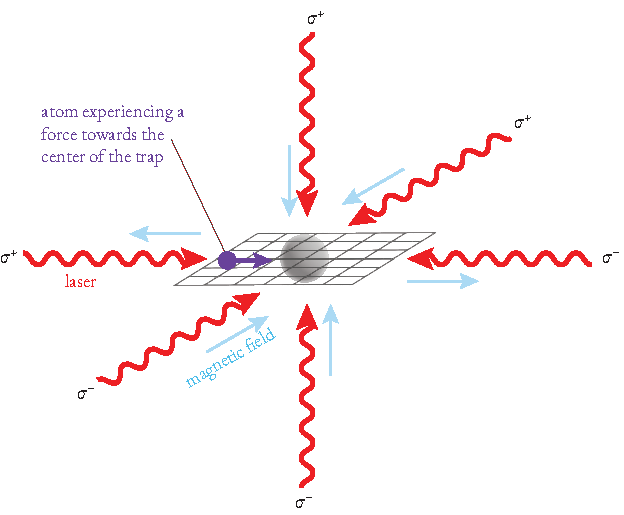
\includegraphics[scale=0.6]{\imagepath/restoring_on_opposite_sides_schematic/restoring_on_opposite_sides_schematic.pdf}
    \end{figure}
    \section{3D MOT}
\end{frame}

\begin{frame}
    \frametitle{Optical Molasses}
    \begin{columns}
        \onslide<+->
        \begin{column}[]{0.48\textwidth}
            \begin{figure}
                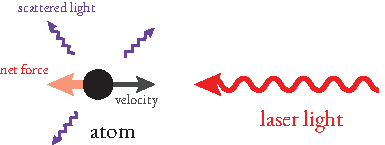
\includegraphics[scale=0.7]{\imagepath/light_scattering_momentum_transfer/light_scattering_momentum_transfer.pdf}
            \end{figure}
        \end{column}
        
        \onslide<+->
        \begin{column}[]{0.48\textwidth}
            \begin{figure}
                \scalebox{0.7}{
                    \begin{pgfpicture}
                        \pgftext{%% Creator: Matplotlib, PGF backend
%%
%% To include the figure in your LaTeX document, write
%%   \input{<filename>.pgf}
%%
%% Make sure the required packages are loaded in your preamble
%%   \usepackage{pgf}
%%
%% Also ensure that all the required font packages are loaded; for instance,
%% the lmodern package is sometimes necessary when using math font.
%%   \usepackage{lmodern}
%%
%% Figures using additional raster images can only be included by \input if
%% they are in the same directory as the main LaTeX file. For loading figures
%% from other directories you can use the `import` package
%%   \usepackage{import}
%%
%% and then include the figures with
%%   \import{<path to file>}{<filename>.pgf}
%%
%% Matplotlib used the following preamble
%%   \usepackage{fontspec}
%%   \setmainfont{DejaVuSerif.ttf}[Path=\detokenize{/home/max/.local/lib/python3.8/site-packages/matplotlib/mpl-data/fonts/ttf/}]
%%   \setsansfont{DejaVuSans.ttf}[Path=\detokenize{/home/max/.local/lib/python3.8/site-packages/matplotlib/mpl-data/fonts/ttf/}]
%%   \setmonofont{DejaVuSansMono.ttf}[Path=\detokenize{/home/max/.local/lib/python3.8/site-packages/matplotlib/mpl-data/fonts/ttf/}]
%%
\begingroup%
\makeatletter%
\begin{pgfpicture}%
\pgfpathrectangle{\pgfpointorigin}{\pgfqpoint{3.825500in}{2.633098in}}%
\pgfusepath{use as bounding box, clip}%
\begin{pgfscope}%
\pgfsetbuttcap%
\pgfsetmiterjoin%
\definecolor{currentfill}{rgb}{1.000000,1.000000,1.000000}%
\pgfsetfillcolor{currentfill}%
\pgfsetlinewidth{0.000000pt}%
\definecolor{currentstroke}{rgb}{1.000000,1.000000,1.000000}%
\pgfsetstrokecolor{currentstroke}%
\pgfsetdash{}{0pt}%
\pgfpathmoveto{\pgfqpoint{0.000000in}{-0.000000in}}%
\pgfpathlineto{\pgfqpoint{3.825500in}{-0.000000in}}%
\pgfpathlineto{\pgfqpoint{3.825500in}{2.633098in}}%
\pgfpathlineto{\pgfqpoint{0.000000in}{2.633098in}}%
\pgfpathlineto{\pgfqpoint{0.000000in}{-0.000000in}}%
\pgfpathclose%
\pgfusepath{fill}%
\end{pgfscope}%
\begin{pgfscope}%
\pgfsetbuttcap%
\pgfsetmiterjoin%
\definecolor{currentfill}{rgb}{1.000000,1.000000,1.000000}%
\pgfsetfillcolor{currentfill}%
\pgfsetlinewidth{0.000000pt}%
\definecolor{currentstroke}{rgb}{0.000000,0.000000,0.000000}%
\pgfsetstrokecolor{currentstroke}%
\pgfsetstrokeopacity{0.000000}%
\pgfsetdash{}{0pt}%
\pgfpathmoveto{\pgfqpoint{0.756020in}{0.499970in}}%
\pgfpathlineto{\pgfqpoint{3.725500in}{0.499970in}}%
\pgfpathlineto{\pgfqpoint{3.725500in}{2.533098in}}%
\pgfpathlineto{\pgfqpoint{0.756020in}{2.533098in}}%
\pgfpathlineto{\pgfqpoint{0.756020in}{0.499970in}}%
\pgfpathclose%
\pgfusepath{fill}%
\end{pgfscope}%
\begin{pgfscope}%
\pgfpathrectangle{\pgfqpoint{0.756020in}{0.499970in}}{\pgfqpoint{2.969480in}{2.033128in}}%
\pgfusepath{clip}%
\pgfsetrectcap%
\pgfsetroundjoin%
\pgfsetlinewidth{0.803000pt}%
\definecolor{currentstroke}{rgb}{0.690196,0.690196,0.690196}%
\pgfsetstrokecolor{currentstroke}%
\pgfsetdash{}{0pt}%
\pgfpathmoveto{\pgfqpoint{0.890997in}{0.499970in}}%
\pgfpathlineto{\pgfqpoint{0.890997in}{2.533098in}}%
\pgfusepath{stroke}%
\end{pgfscope}%
\begin{pgfscope}%
\pgfsetbuttcap%
\pgfsetroundjoin%
\definecolor{currentfill}{rgb}{0.000000,0.000000,0.000000}%
\pgfsetfillcolor{currentfill}%
\pgfsetlinewidth{0.803000pt}%
\definecolor{currentstroke}{rgb}{0.000000,0.000000,0.000000}%
\pgfsetstrokecolor{currentstroke}%
\pgfsetdash{}{0pt}%
\pgfsys@defobject{currentmarker}{\pgfqpoint{0.000000in}{-0.048611in}}{\pgfqpoint{0.000000in}{0.000000in}}{%
\pgfpathmoveto{\pgfqpoint{0.000000in}{0.000000in}}%
\pgfpathlineto{\pgfqpoint{0.000000in}{-0.048611in}}%
\pgfusepath{stroke,fill}%
}%
\begin{pgfscope}%
\pgfsys@transformshift{0.890997in}{0.499970in}%
\pgfsys@useobject{currentmarker}{}%
\end{pgfscope}%
\end{pgfscope}%
\begin{pgfscope}%
\definecolor{textcolor}{rgb}{0.000000,0.000000,0.000000}%
\pgfsetstrokecolor{textcolor}%
\pgfsetfillcolor{textcolor}%
\pgftext[x=0.890997in,y=0.402748in,,top]{\color{textcolor}\rmfamily\fontsize{9.000000}{10.800000}\selectfont \ensuremath{-}2}%
\end{pgfscope}%
\begin{pgfscope}%
\pgfpathrectangle{\pgfqpoint{0.756020in}{0.499970in}}{\pgfqpoint{2.969480in}{2.033128in}}%
\pgfusepath{clip}%
\pgfsetrectcap%
\pgfsetroundjoin%
\pgfsetlinewidth{0.803000pt}%
\definecolor{currentstroke}{rgb}{0.690196,0.690196,0.690196}%
\pgfsetstrokecolor{currentstroke}%
\pgfsetdash{}{0pt}%
\pgfpathmoveto{\pgfqpoint{1.565878in}{0.499970in}}%
\pgfpathlineto{\pgfqpoint{1.565878in}{2.533098in}}%
\pgfusepath{stroke}%
\end{pgfscope}%
\begin{pgfscope}%
\pgfsetbuttcap%
\pgfsetroundjoin%
\definecolor{currentfill}{rgb}{0.000000,0.000000,0.000000}%
\pgfsetfillcolor{currentfill}%
\pgfsetlinewidth{0.803000pt}%
\definecolor{currentstroke}{rgb}{0.000000,0.000000,0.000000}%
\pgfsetstrokecolor{currentstroke}%
\pgfsetdash{}{0pt}%
\pgfsys@defobject{currentmarker}{\pgfqpoint{0.000000in}{-0.048611in}}{\pgfqpoint{0.000000in}{0.000000in}}{%
\pgfpathmoveto{\pgfqpoint{0.000000in}{0.000000in}}%
\pgfpathlineto{\pgfqpoint{0.000000in}{-0.048611in}}%
\pgfusepath{stroke,fill}%
}%
\begin{pgfscope}%
\pgfsys@transformshift{1.565878in}{0.499970in}%
\pgfsys@useobject{currentmarker}{}%
\end{pgfscope}%
\end{pgfscope}%
\begin{pgfscope}%
\definecolor{textcolor}{rgb}{0.000000,0.000000,0.000000}%
\pgfsetstrokecolor{textcolor}%
\pgfsetfillcolor{textcolor}%
\pgftext[x=1.565878in,y=0.402748in,,top]{\color{textcolor}\rmfamily\fontsize{9.000000}{10.800000}\selectfont \ensuremath{-}1}%
\end{pgfscope}%
\begin{pgfscope}%
\pgfpathrectangle{\pgfqpoint{0.756020in}{0.499970in}}{\pgfqpoint{2.969480in}{2.033128in}}%
\pgfusepath{clip}%
\pgfsetrectcap%
\pgfsetroundjoin%
\pgfsetlinewidth{0.803000pt}%
\definecolor{currentstroke}{rgb}{0.690196,0.690196,0.690196}%
\pgfsetstrokecolor{currentstroke}%
\pgfsetdash{}{0pt}%
\pgfpathmoveto{\pgfqpoint{2.240760in}{0.499970in}}%
\pgfpathlineto{\pgfqpoint{2.240760in}{2.533098in}}%
\pgfusepath{stroke}%
\end{pgfscope}%
\begin{pgfscope}%
\pgfsetbuttcap%
\pgfsetroundjoin%
\definecolor{currentfill}{rgb}{0.000000,0.000000,0.000000}%
\pgfsetfillcolor{currentfill}%
\pgfsetlinewidth{0.803000pt}%
\definecolor{currentstroke}{rgb}{0.000000,0.000000,0.000000}%
\pgfsetstrokecolor{currentstroke}%
\pgfsetdash{}{0pt}%
\pgfsys@defobject{currentmarker}{\pgfqpoint{0.000000in}{-0.048611in}}{\pgfqpoint{0.000000in}{0.000000in}}{%
\pgfpathmoveto{\pgfqpoint{0.000000in}{0.000000in}}%
\pgfpathlineto{\pgfqpoint{0.000000in}{-0.048611in}}%
\pgfusepath{stroke,fill}%
}%
\begin{pgfscope}%
\pgfsys@transformshift{2.240760in}{0.499970in}%
\pgfsys@useobject{currentmarker}{}%
\end{pgfscope}%
\end{pgfscope}%
\begin{pgfscope}%
\definecolor{textcolor}{rgb}{0.000000,0.000000,0.000000}%
\pgfsetstrokecolor{textcolor}%
\pgfsetfillcolor{textcolor}%
\pgftext[x=2.240760in,y=0.402748in,,top]{\color{textcolor}\rmfamily\fontsize{9.000000}{10.800000}\selectfont 0}%
\end{pgfscope}%
\begin{pgfscope}%
\pgfpathrectangle{\pgfqpoint{0.756020in}{0.499970in}}{\pgfqpoint{2.969480in}{2.033128in}}%
\pgfusepath{clip}%
\pgfsetrectcap%
\pgfsetroundjoin%
\pgfsetlinewidth{0.803000pt}%
\definecolor{currentstroke}{rgb}{0.690196,0.690196,0.690196}%
\pgfsetstrokecolor{currentstroke}%
\pgfsetdash{}{0pt}%
\pgfpathmoveto{\pgfqpoint{2.915642in}{0.499970in}}%
\pgfpathlineto{\pgfqpoint{2.915642in}{2.533098in}}%
\pgfusepath{stroke}%
\end{pgfscope}%
\begin{pgfscope}%
\pgfsetbuttcap%
\pgfsetroundjoin%
\definecolor{currentfill}{rgb}{0.000000,0.000000,0.000000}%
\pgfsetfillcolor{currentfill}%
\pgfsetlinewidth{0.803000pt}%
\definecolor{currentstroke}{rgb}{0.000000,0.000000,0.000000}%
\pgfsetstrokecolor{currentstroke}%
\pgfsetdash{}{0pt}%
\pgfsys@defobject{currentmarker}{\pgfqpoint{0.000000in}{-0.048611in}}{\pgfqpoint{0.000000in}{0.000000in}}{%
\pgfpathmoveto{\pgfqpoint{0.000000in}{0.000000in}}%
\pgfpathlineto{\pgfqpoint{0.000000in}{-0.048611in}}%
\pgfusepath{stroke,fill}%
}%
\begin{pgfscope}%
\pgfsys@transformshift{2.915642in}{0.499970in}%
\pgfsys@useobject{currentmarker}{}%
\end{pgfscope}%
\end{pgfscope}%
\begin{pgfscope}%
\definecolor{textcolor}{rgb}{0.000000,0.000000,0.000000}%
\pgfsetstrokecolor{textcolor}%
\pgfsetfillcolor{textcolor}%
\pgftext[x=2.915642in,y=0.402748in,,top]{\color{textcolor}\rmfamily\fontsize{9.000000}{10.800000}\selectfont 1}%
\end{pgfscope}%
\begin{pgfscope}%
\pgfpathrectangle{\pgfqpoint{0.756020in}{0.499970in}}{\pgfqpoint{2.969480in}{2.033128in}}%
\pgfusepath{clip}%
\pgfsetrectcap%
\pgfsetroundjoin%
\pgfsetlinewidth{0.803000pt}%
\definecolor{currentstroke}{rgb}{0.690196,0.690196,0.690196}%
\pgfsetstrokecolor{currentstroke}%
\pgfsetdash{}{0pt}%
\pgfpathmoveto{\pgfqpoint{3.590524in}{0.499970in}}%
\pgfpathlineto{\pgfqpoint{3.590524in}{2.533098in}}%
\pgfusepath{stroke}%
\end{pgfscope}%
\begin{pgfscope}%
\pgfsetbuttcap%
\pgfsetroundjoin%
\definecolor{currentfill}{rgb}{0.000000,0.000000,0.000000}%
\pgfsetfillcolor{currentfill}%
\pgfsetlinewidth{0.803000pt}%
\definecolor{currentstroke}{rgb}{0.000000,0.000000,0.000000}%
\pgfsetstrokecolor{currentstroke}%
\pgfsetdash{}{0pt}%
\pgfsys@defobject{currentmarker}{\pgfqpoint{0.000000in}{-0.048611in}}{\pgfqpoint{0.000000in}{0.000000in}}{%
\pgfpathmoveto{\pgfqpoint{0.000000in}{0.000000in}}%
\pgfpathlineto{\pgfqpoint{0.000000in}{-0.048611in}}%
\pgfusepath{stroke,fill}%
}%
\begin{pgfscope}%
\pgfsys@transformshift{3.590524in}{0.499970in}%
\pgfsys@useobject{currentmarker}{}%
\end{pgfscope}%
\end{pgfscope}%
\begin{pgfscope}%
\definecolor{textcolor}{rgb}{0.000000,0.000000,0.000000}%
\pgfsetstrokecolor{textcolor}%
\pgfsetfillcolor{textcolor}%
\pgftext[x=3.590524in,y=0.402748in,,top]{\color{textcolor}\rmfamily\fontsize{9.000000}{10.800000}\selectfont 2}%
\end{pgfscope}%
\begin{pgfscope}%
\definecolor{textcolor}{rgb}{0.000000,0.000000,0.000000}%
\pgfsetstrokecolor{textcolor}%
\pgfsetfillcolor{textcolor}%
\pgftext[x=2.240760in,y=0.226221in,,top]{\color{textcolor}\rmfamily\fontsize{9.000000}{10.800000}\selectfont speed in \(\displaystyle \Gamma/k\)}%
\end{pgfscope}%
\begin{pgfscope}%
\pgfpathrectangle{\pgfqpoint{0.756020in}{0.499970in}}{\pgfqpoint{2.969480in}{2.033128in}}%
\pgfusepath{clip}%
\pgfsetrectcap%
\pgfsetroundjoin%
\pgfsetlinewidth{0.803000pt}%
\definecolor{currentstroke}{rgb}{0.690196,0.690196,0.690196}%
\pgfsetstrokecolor{currentstroke}%
\pgfsetdash{}{0pt}%
\pgfpathmoveto{\pgfqpoint{0.756020in}{0.678437in}}%
\pgfpathlineto{\pgfqpoint{3.725500in}{0.678437in}}%
\pgfusepath{stroke}%
\end{pgfscope}%
\begin{pgfscope}%
\pgfsetbuttcap%
\pgfsetroundjoin%
\definecolor{currentfill}{rgb}{0.000000,0.000000,0.000000}%
\pgfsetfillcolor{currentfill}%
\pgfsetlinewidth{0.803000pt}%
\definecolor{currentstroke}{rgb}{0.000000,0.000000,0.000000}%
\pgfsetstrokecolor{currentstroke}%
\pgfsetdash{}{0pt}%
\pgfsys@defobject{currentmarker}{\pgfqpoint{-0.048611in}{0.000000in}}{\pgfqpoint{-0.000000in}{0.000000in}}{%
\pgfpathmoveto{\pgfqpoint{-0.000000in}{0.000000in}}%
\pgfpathlineto{\pgfqpoint{-0.048611in}{0.000000in}}%
\pgfusepath{stroke,fill}%
}%
\begin{pgfscope}%
\pgfsys@transformshift{0.756020in}{0.678437in}%
\pgfsys@useobject{currentmarker}{}%
\end{pgfscope}%
\end{pgfscope}%
\begin{pgfscope}%
\definecolor{textcolor}{rgb}{0.000000,0.000000,0.000000}%
\pgfsetstrokecolor{textcolor}%
\pgfsetfillcolor{textcolor}%
\pgftext[x=0.280556in, y=0.630952in, left, base]{\color{textcolor}\rmfamily\fontsize{9.000000}{10.800000}\selectfont \ensuremath{-}0.04}%
\end{pgfscope}%
\begin{pgfscope}%
\pgfpathrectangle{\pgfqpoint{0.756020in}{0.499970in}}{\pgfqpoint{2.969480in}{2.033128in}}%
\pgfusepath{clip}%
\pgfsetrectcap%
\pgfsetroundjoin%
\pgfsetlinewidth{0.803000pt}%
\definecolor{currentstroke}{rgb}{0.690196,0.690196,0.690196}%
\pgfsetstrokecolor{currentstroke}%
\pgfsetdash{}{0pt}%
\pgfpathmoveto{\pgfqpoint{0.756020in}{1.097486in}}%
\pgfpathlineto{\pgfqpoint{3.725500in}{1.097486in}}%
\pgfusepath{stroke}%
\end{pgfscope}%
\begin{pgfscope}%
\pgfsetbuttcap%
\pgfsetroundjoin%
\definecolor{currentfill}{rgb}{0.000000,0.000000,0.000000}%
\pgfsetfillcolor{currentfill}%
\pgfsetlinewidth{0.803000pt}%
\definecolor{currentstroke}{rgb}{0.000000,0.000000,0.000000}%
\pgfsetstrokecolor{currentstroke}%
\pgfsetdash{}{0pt}%
\pgfsys@defobject{currentmarker}{\pgfqpoint{-0.048611in}{0.000000in}}{\pgfqpoint{-0.000000in}{0.000000in}}{%
\pgfpathmoveto{\pgfqpoint{-0.000000in}{0.000000in}}%
\pgfpathlineto{\pgfqpoint{-0.048611in}{0.000000in}}%
\pgfusepath{stroke,fill}%
}%
\begin{pgfscope}%
\pgfsys@transformshift{0.756020in}{1.097486in}%
\pgfsys@useobject{currentmarker}{}%
\end{pgfscope}%
\end{pgfscope}%
\begin{pgfscope}%
\definecolor{textcolor}{rgb}{0.000000,0.000000,0.000000}%
\pgfsetstrokecolor{textcolor}%
\pgfsetfillcolor{textcolor}%
\pgftext[x=0.280556in, y=1.050000in, left, base]{\color{textcolor}\rmfamily\fontsize{9.000000}{10.800000}\selectfont \ensuremath{-}0.02}%
\end{pgfscope}%
\begin{pgfscope}%
\pgfpathrectangle{\pgfqpoint{0.756020in}{0.499970in}}{\pgfqpoint{2.969480in}{2.033128in}}%
\pgfusepath{clip}%
\pgfsetrectcap%
\pgfsetroundjoin%
\pgfsetlinewidth{0.803000pt}%
\definecolor{currentstroke}{rgb}{0.690196,0.690196,0.690196}%
\pgfsetstrokecolor{currentstroke}%
\pgfsetdash{}{0pt}%
\pgfpathmoveto{\pgfqpoint{0.756020in}{1.516534in}}%
\pgfpathlineto{\pgfqpoint{3.725500in}{1.516534in}}%
\pgfusepath{stroke}%
\end{pgfscope}%
\begin{pgfscope}%
\pgfsetbuttcap%
\pgfsetroundjoin%
\definecolor{currentfill}{rgb}{0.000000,0.000000,0.000000}%
\pgfsetfillcolor{currentfill}%
\pgfsetlinewidth{0.803000pt}%
\definecolor{currentstroke}{rgb}{0.000000,0.000000,0.000000}%
\pgfsetstrokecolor{currentstroke}%
\pgfsetdash{}{0pt}%
\pgfsys@defobject{currentmarker}{\pgfqpoint{-0.048611in}{0.000000in}}{\pgfqpoint{-0.000000in}{0.000000in}}{%
\pgfpathmoveto{\pgfqpoint{-0.000000in}{0.000000in}}%
\pgfpathlineto{\pgfqpoint{-0.048611in}{0.000000in}}%
\pgfusepath{stroke,fill}%
}%
\begin{pgfscope}%
\pgfsys@transformshift{0.756020in}{1.516534in}%
\pgfsys@useobject{currentmarker}{}%
\end{pgfscope}%
\end{pgfscope}%
\begin{pgfscope}%
\definecolor{textcolor}{rgb}{0.000000,0.000000,0.000000}%
\pgfsetstrokecolor{textcolor}%
\pgfsetfillcolor{textcolor}%
\pgftext[x=0.380478in, y=1.469049in, left, base]{\color{textcolor}\rmfamily\fontsize{9.000000}{10.800000}\selectfont 0.00}%
\end{pgfscope}%
\begin{pgfscope}%
\pgfpathrectangle{\pgfqpoint{0.756020in}{0.499970in}}{\pgfqpoint{2.969480in}{2.033128in}}%
\pgfusepath{clip}%
\pgfsetrectcap%
\pgfsetroundjoin%
\pgfsetlinewidth{0.803000pt}%
\definecolor{currentstroke}{rgb}{0.690196,0.690196,0.690196}%
\pgfsetstrokecolor{currentstroke}%
\pgfsetdash{}{0pt}%
\pgfpathmoveto{\pgfqpoint{0.756020in}{1.935582in}}%
\pgfpathlineto{\pgfqpoint{3.725500in}{1.935582in}}%
\pgfusepath{stroke}%
\end{pgfscope}%
\begin{pgfscope}%
\pgfsetbuttcap%
\pgfsetroundjoin%
\definecolor{currentfill}{rgb}{0.000000,0.000000,0.000000}%
\pgfsetfillcolor{currentfill}%
\pgfsetlinewidth{0.803000pt}%
\definecolor{currentstroke}{rgb}{0.000000,0.000000,0.000000}%
\pgfsetstrokecolor{currentstroke}%
\pgfsetdash{}{0pt}%
\pgfsys@defobject{currentmarker}{\pgfqpoint{-0.048611in}{0.000000in}}{\pgfqpoint{-0.000000in}{0.000000in}}{%
\pgfpathmoveto{\pgfqpoint{-0.000000in}{0.000000in}}%
\pgfpathlineto{\pgfqpoint{-0.048611in}{0.000000in}}%
\pgfusepath{stroke,fill}%
}%
\begin{pgfscope}%
\pgfsys@transformshift{0.756020in}{1.935582in}%
\pgfsys@useobject{currentmarker}{}%
\end{pgfscope}%
\end{pgfscope}%
\begin{pgfscope}%
\definecolor{textcolor}{rgb}{0.000000,0.000000,0.000000}%
\pgfsetstrokecolor{textcolor}%
\pgfsetfillcolor{textcolor}%
\pgftext[x=0.380478in, y=1.888097in, left, base]{\color{textcolor}\rmfamily\fontsize{9.000000}{10.800000}\selectfont 0.02}%
\end{pgfscope}%
\begin{pgfscope}%
\pgfpathrectangle{\pgfqpoint{0.756020in}{0.499970in}}{\pgfqpoint{2.969480in}{2.033128in}}%
\pgfusepath{clip}%
\pgfsetrectcap%
\pgfsetroundjoin%
\pgfsetlinewidth{0.803000pt}%
\definecolor{currentstroke}{rgb}{0.690196,0.690196,0.690196}%
\pgfsetstrokecolor{currentstroke}%
\pgfsetdash{}{0pt}%
\pgfpathmoveto{\pgfqpoint{0.756020in}{2.354630in}}%
\pgfpathlineto{\pgfqpoint{3.725500in}{2.354630in}}%
\pgfusepath{stroke}%
\end{pgfscope}%
\begin{pgfscope}%
\pgfsetbuttcap%
\pgfsetroundjoin%
\definecolor{currentfill}{rgb}{0.000000,0.000000,0.000000}%
\pgfsetfillcolor{currentfill}%
\pgfsetlinewidth{0.803000pt}%
\definecolor{currentstroke}{rgb}{0.000000,0.000000,0.000000}%
\pgfsetstrokecolor{currentstroke}%
\pgfsetdash{}{0pt}%
\pgfsys@defobject{currentmarker}{\pgfqpoint{-0.048611in}{0.000000in}}{\pgfqpoint{-0.000000in}{0.000000in}}{%
\pgfpathmoveto{\pgfqpoint{-0.000000in}{0.000000in}}%
\pgfpathlineto{\pgfqpoint{-0.048611in}{0.000000in}}%
\pgfusepath{stroke,fill}%
}%
\begin{pgfscope}%
\pgfsys@transformshift{0.756020in}{2.354630in}%
\pgfsys@useobject{currentmarker}{}%
\end{pgfscope}%
\end{pgfscope}%
\begin{pgfscope}%
\definecolor{textcolor}{rgb}{0.000000,0.000000,0.000000}%
\pgfsetstrokecolor{textcolor}%
\pgfsetfillcolor{textcolor}%
\pgftext[x=0.380478in, y=2.307145in, left, base]{\color{textcolor}\rmfamily\fontsize{9.000000}{10.800000}\selectfont 0.04}%
\end{pgfscope}%
\begin{pgfscope}%
\definecolor{textcolor}{rgb}{0.000000,0.000000,0.000000}%
\pgfsetstrokecolor{textcolor}%
\pgfsetfillcolor{textcolor}%
\pgftext[x=0.225000in,y=1.516534in,,bottom,rotate=90.000000]{\color{textcolor}\rmfamily\fontsize{9.000000}{10.800000}\selectfont \(\displaystyle F_\mathrm{MO}\) in \(\displaystyle 1/(\hbar k \Gamma)\)}%
\end{pgfscope}%
\begin{pgfscope}%
\pgfpathrectangle{\pgfqpoint{0.756020in}{0.499970in}}{\pgfqpoint{2.969480in}{2.033128in}}%
\pgfusepath{clip}%
\pgfsetrectcap%
\pgfsetroundjoin%
\pgfsetlinewidth{1.505625pt}%
\definecolor{currentstroke}{rgb}{1.000000,0.000000,0.000000}%
\pgfsetstrokecolor{currentstroke}%
\pgfsetstrokeopacity{0.120000}%
\pgfsetdash{}{0pt}%
\pgfpathmoveto{\pgfqpoint{0.890997in}{1.994490in}}%
\pgfpathlineto{\pgfqpoint{0.927111in}{2.047116in}}%
\pgfpathlineto{\pgfqpoint{0.963225in}{2.104204in}}%
\pgfpathlineto{\pgfqpoint{1.008367in}{2.180249in}}%
\pgfpathlineto{\pgfqpoint{1.080596in}{2.302793in}}%
\pgfpathlineto{\pgfqpoint{1.107681in}{2.344371in}}%
\pgfpathlineto{\pgfqpoint{1.125738in}{2.369299in}}%
\pgfpathlineto{\pgfqpoint{1.143795in}{2.391311in}}%
\pgfpathlineto{\pgfqpoint{1.161852in}{2.409840in}}%
\pgfpathlineto{\pgfqpoint{1.179909in}{2.424372in}}%
\pgfpathlineto{\pgfqpoint{1.197966in}{2.434478in}}%
\pgfpathlineto{\pgfqpoint{1.206995in}{2.437767in}}%
\pgfpathlineto{\pgfqpoint{1.216023in}{2.439841in}}%
\pgfpathlineto{\pgfqpoint{1.225052in}{2.440683in}}%
\pgfpathlineto{\pgfqpoint{1.234080in}{2.440283in}}%
\pgfpathlineto{\pgfqpoint{1.243109in}{2.438643in}}%
\pgfpathlineto{\pgfqpoint{1.252137in}{2.435774in}}%
\pgfpathlineto{\pgfqpoint{1.270194in}{2.426438in}}%
\pgfpathlineto{\pgfqpoint{1.288252in}{2.412540in}}%
\pgfpathlineto{\pgfqpoint{1.306309in}{2.394469in}}%
\pgfpathlineto{\pgfqpoint{1.324366in}{2.372712in}}%
\pgfpathlineto{\pgfqpoint{1.342423in}{2.347817in}}%
\pgfpathlineto{\pgfqpoint{1.369508in}{2.305866in}}%
\pgfpathlineto{\pgfqpoint{1.405622in}{2.244332in}}%
\pgfpathlineto{\pgfqpoint{1.504936in}{2.070441in}}%
\pgfpathlineto{\pgfqpoint{1.541050in}{2.012480in}}%
\pgfpathlineto{\pgfqpoint{1.577164in}{1.959094in}}%
\pgfpathlineto{\pgfqpoint{1.613278in}{1.910533in}}%
\pgfpathlineto{\pgfqpoint{1.649392in}{1.866706in}}%
\pgfpathlineto{\pgfqpoint{1.685506in}{1.827319in}}%
\pgfpathlineto{\pgfqpoint{1.721620in}{1.791981in}}%
\pgfpathlineto{\pgfqpoint{1.757735in}{1.760260in}}%
\pgfpathlineto{\pgfqpoint{1.793849in}{1.731724in}}%
\pgfpathlineto{\pgfqpoint{1.829963in}{1.705967in}}%
\pgfpathlineto{\pgfqpoint{1.866077in}{1.682613in}}%
\pgfpathlineto{\pgfqpoint{1.911219in}{1.656284in}}%
\pgfpathlineto{\pgfqpoint{1.956362in}{1.632594in}}%
\pgfpathlineto{\pgfqpoint{2.010533in}{1.606942in}}%
\pgfpathlineto{\pgfqpoint{2.073733in}{1.579902in}}%
\pgfpathlineto{\pgfqpoint{2.145961in}{1.551582in}}%
\pgfpathlineto{\pgfqpoint{2.272360in}{1.504978in}}%
\pgfpathlineto{\pgfqpoint{2.380702in}{1.464042in}}%
\pgfpathlineto{\pgfqpoint{2.443902in}{1.438039in}}%
\pgfpathlineto{\pgfqpoint{2.498073in}{1.413634in}}%
\pgfpathlineto{\pgfqpoint{2.543216in}{1.391280in}}%
\pgfpathlineto{\pgfqpoint{2.588358in}{1.366600in}}%
\pgfpathlineto{\pgfqpoint{2.633501in}{1.339056in}}%
\pgfpathlineto{\pgfqpoint{2.669615in}{1.314545in}}%
\pgfpathlineto{\pgfqpoint{2.705729in}{1.287448in}}%
\pgfpathlineto{\pgfqpoint{2.741843in}{1.257372in}}%
\pgfpathlineto{\pgfqpoint{2.777957in}{1.223897in}}%
\pgfpathlineto{\pgfqpoint{2.814071in}{1.186587in}}%
\pgfpathlineto{\pgfqpoint{2.841157in}{1.155835in}}%
\pgfpathlineto{\pgfqpoint{2.868242in}{1.122535in}}%
\pgfpathlineto{\pgfqpoint{2.904357in}{1.073974in}}%
\pgfpathlineto{\pgfqpoint{2.940471in}{1.020588in}}%
\pgfpathlineto{\pgfqpoint{2.976585in}{0.962627in}}%
\pgfpathlineto{\pgfqpoint{3.021727in}{0.884994in}}%
\pgfpathlineto{\pgfqpoint{3.112012in}{0.727201in}}%
\pgfpathlineto{\pgfqpoint{3.139098in}{0.685251in}}%
\pgfpathlineto{\pgfqpoint{3.157155in}{0.660356in}}%
\pgfpathlineto{\pgfqpoint{3.175212in}{0.638598in}}%
\pgfpathlineto{\pgfqpoint{3.193269in}{0.620528in}}%
\pgfpathlineto{\pgfqpoint{3.211326in}{0.606630in}}%
\pgfpathlineto{\pgfqpoint{3.229383in}{0.597293in}}%
\pgfpathlineto{\pgfqpoint{3.238412in}{0.594424in}}%
\pgfpathlineto{\pgfqpoint{3.247440in}{0.592785in}}%
\pgfpathlineto{\pgfqpoint{3.256469in}{0.592385in}}%
\pgfpathlineto{\pgfqpoint{3.265497in}{0.593226in}}%
\pgfpathlineto{\pgfqpoint{3.274526in}{0.595301in}}%
\pgfpathlineto{\pgfqpoint{3.283554in}{0.598590in}}%
\pgfpathlineto{\pgfqpoint{3.301611in}{0.608696in}}%
\pgfpathlineto{\pgfqpoint{3.319668in}{0.623228in}}%
\pgfpathlineto{\pgfqpoint{3.337725in}{0.641757in}}%
\pgfpathlineto{\pgfqpoint{3.355782in}{0.663769in}}%
\pgfpathlineto{\pgfqpoint{3.373840in}{0.688697in}}%
\pgfpathlineto{\pgfqpoint{3.400925in}{0.730275in}}%
\pgfpathlineto{\pgfqpoint{3.437039in}{0.790571in}}%
\pgfpathlineto{\pgfqpoint{3.527324in}{0.943512in}}%
\pgfpathlineto{\pgfqpoint{3.563438in}{0.999550in}}%
\pgfpathlineto{\pgfqpoint{3.590524in}{1.038577in}}%
\pgfpathlineto{\pgfqpoint{3.590524in}{1.038577in}}%
\pgfusepath{stroke}%
\end{pgfscope}%
\begin{pgfscope}%
\pgfpathrectangle{\pgfqpoint{0.756020in}{0.499970in}}{\pgfqpoint{2.969480in}{2.033128in}}%
\pgfusepath{clip}%
\pgfsetrectcap%
\pgfsetroundjoin%
\pgfsetlinewidth{1.505625pt}%
\definecolor{currentstroke}{rgb}{1.000000,0.000000,0.000000}%
\pgfsetstrokecolor{currentstroke}%
\pgfsetstrokeopacity{0.480000}%
\pgfsetdash{}{0pt}%
\pgfpathmoveto{\pgfqpoint{0.890997in}{1.693712in}}%
\pgfpathlineto{\pgfqpoint{0.927111in}{1.710983in}}%
\pgfpathlineto{\pgfqpoint{0.963225in}{1.730458in}}%
\pgfpathlineto{\pgfqpoint{0.999339in}{1.752453in}}%
\pgfpathlineto{\pgfqpoint{1.035453in}{1.777323in}}%
\pgfpathlineto{\pgfqpoint{1.071567in}{1.805455in}}%
\pgfpathlineto{\pgfqpoint{1.107681in}{1.837262in}}%
\pgfpathlineto{\pgfqpoint{1.134767in}{1.863779in}}%
\pgfpathlineto{\pgfqpoint{1.161852in}{1.892761in}}%
\pgfpathlineto{\pgfqpoint{1.188938in}{1.924348in}}%
\pgfpathlineto{\pgfqpoint{1.216023in}{1.958635in}}%
\pgfpathlineto{\pgfqpoint{1.252137in}{2.008579in}}%
\pgfpathlineto{\pgfqpoint{1.288252in}{2.063102in}}%
\pgfpathlineto{\pgfqpoint{1.333394in}{2.136451in}}%
\pgfpathlineto{\pgfqpoint{1.423679in}{2.285801in}}%
\pgfpathlineto{\pgfqpoint{1.450765in}{2.325275in}}%
\pgfpathlineto{\pgfqpoint{1.468822in}{2.348531in}}%
\pgfpathlineto{\pgfqpoint{1.486879in}{2.368657in}}%
\pgfpathlineto{\pgfqpoint{1.504936in}{2.385098in}}%
\pgfpathlineto{\pgfqpoint{1.522993in}{2.397360in}}%
\pgfpathlineto{\pgfqpoint{1.541050in}{2.405044in}}%
\pgfpathlineto{\pgfqpoint{1.550079in}{2.407078in}}%
\pgfpathlineto{\pgfqpoint{1.559107in}{2.407875in}}%
\pgfpathlineto{\pgfqpoint{1.568136in}{2.407421in}}%
\pgfpathlineto{\pgfqpoint{1.577164in}{2.405715in}}%
\pgfpathlineto{\pgfqpoint{1.586193in}{2.402763in}}%
\pgfpathlineto{\pgfqpoint{1.604250in}{2.393196in}}%
\pgfpathlineto{\pgfqpoint{1.622307in}{2.378959in}}%
\pgfpathlineto{\pgfqpoint{1.640364in}{2.360417in}}%
\pgfpathlineto{\pgfqpoint{1.658421in}{2.338036in}}%
\pgfpathlineto{\pgfqpoint{1.676478in}{2.312355in}}%
\pgfpathlineto{\pgfqpoint{1.703563in}{2.268903in}}%
\pgfpathlineto{\pgfqpoint{1.739677in}{2.204770in}}%
\pgfpathlineto{\pgfqpoint{1.866077in}{1.973174in}}%
\pgfpathlineto{\pgfqpoint{1.902191in}{1.913473in}}%
\pgfpathlineto{\pgfqpoint{1.938305in}{1.858056in}}%
\pgfpathlineto{\pgfqpoint{1.974419in}{1.806863in}}%
\pgfpathlineto{\pgfqpoint{2.010533in}{1.759581in}}%
\pgfpathlineto{\pgfqpoint{2.046647in}{1.715754in}}%
\pgfpathlineto{\pgfqpoint{2.091790in}{1.665022in}}%
\pgfpathlineto{\pgfqpoint{2.136932in}{1.617781in}}%
\pgfpathlineto{\pgfqpoint{2.200132in}{1.555455in}}%
\pgfpathlineto{\pgfqpoint{2.344588in}{1.415286in}}%
\pgfpathlineto{\pgfqpoint{2.389731in}{1.368046in}}%
\pgfpathlineto{\pgfqpoint{2.434873in}{1.317314in}}%
\pgfpathlineto{\pgfqpoint{2.470988in}{1.273487in}}%
\pgfpathlineto{\pgfqpoint{2.507102in}{1.226205in}}%
\pgfpathlineto{\pgfqpoint{2.543216in}{1.175012in}}%
\pgfpathlineto{\pgfqpoint{2.579330in}{1.119594in}}%
\pgfpathlineto{\pgfqpoint{2.615444in}{1.059893in}}%
\pgfpathlineto{\pgfqpoint{2.651558in}{0.996259in}}%
\pgfpathlineto{\pgfqpoint{2.705729in}{0.895743in}}%
\pgfpathlineto{\pgfqpoint{2.759900in}{0.795575in}}%
\pgfpathlineto{\pgfqpoint{2.786986in}{0.749121in}}%
\pgfpathlineto{\pgfqpoint{2.814071in}{0.707495in}}%
\pgfpathlineto{\pgfqpoint{2.832128in}{0.683394in}}%
\pgfpathlineto{\pgfqpoint{2.850185in}{0.662869in}}%
\pgfpathlineto{\pgfqpoint{2.868242in}{0.646427in}}%
\pgfpathlineto{\pgfqpoint{2.886299in}{0.634486in}}%
\pgfpathlineto{\pgfqpoint{2.895328in}{0.630305in}}%
\pgfpathlineto{\pgfqpoint{2.904357in}{0.627353in}}%
\pgfpathlineto{\pgfqpoint{2.913385in}{0.625647in}}%
\pgfpathlineto{\pgfqpoint{2.922414in}{0.625193in}}%
\pgfpathlineto{\pgfqpoint{2.931442in}{0.625989in}}%
\pgfpathlineto{\pgfqpoint{2.940471in}{0.628023in}}%
\pgfpathlineto{\pgfqpoint{2.949499in}{0.631273in}}%
\pgfpathlineto{\pgfqpoint{2.967556in}{0.641289in}}%
\pgfpathlineto{\pgfqpoint{2.985613in}{0.655697in}}%
\pgfpathlineto{\pgfqpoint{3.003670in}{0.674047in}}%
\pgfpathlineto{\pgfqpoint{3.021727in}{0.695810in}}%
\pgfpathlineto{\pgfqpoint{3.048813in}{0.733595in}}%
\pgfpathlineto{\pgfqpoint{3.075898in}{0.775794in}}%
\pgfpathlineto{\pgfqpoint{3.121041in}{0.851008in}}%
\pgfpathlineto{\pgfqpoint{3.184241in}{0.955695in}}%
\pgfpathlineto{\pgfqpoint{3.220355in}{1.011268in}}%
\pgfpathlineto{\pgfqpoint{3.256469in}{1.062397in}}%
\pgfpathlineto{\pgfqpoint{3.292583in}{1.108720in}}%
\pgfpathlineto{\pgfqpoint{3.319668in}{1.140306in}}%
\pgfpathlineto{\pgfqpoint{3.346754in}{1.169288in}}%
\pgfpathlineto{\pgfqpoint{3.373840in}{1.195805in}}%
\pgfpathlineto{\pgfqpoint{3.409954in}{1.227613in}}%
\pgfpathlineto{\pgfqpoint{3.446068in}{1.255745in}}%
\pgfpathlineto{\pgfqpoint{3.482182in}{1.280615in}}%
\pgfpathlineto{\pgfqpoint{3.518296in}{1.302610in}}%
\pgfpathlineto{\pgfqpoint{3.554410in}{1.322085in}}%
\pgfpathlineto{\pgfqpoint{3.590524in}{1.339356in}}%
\pgfpathlineto{\pgfqpoint{3.590524in}{1.339356in}}%
\pgfusepath{stroke}%
\end{pgfscope}%
\begin{pgfscope}%
\pgfpathrectangle{\pgfqpoint{0.756020in}{0.499970in}}{\pgfqpoint{2.969480in}{2.033128in}}%
\pgfusepath{clip}%
\pgfsetrectcap%
\pgfsetroundjoin%
\pgfsetlinewidth{1.505625pt}%
\definecolor{currentstroke}{rgb}{1.000000,0.000000,0.000000}%
\pgfsetstrokecolor{currentstroke}%
\pgfsetstrokeopacity{0.840000}%
\pgfsetdash{}{0pt}%
\pgfpathmoveto{\pgfqpoint{0.890997in}{1.580120in}}%
\pgfpathlineto{\pgfqpoint{0.963225in}{1.591114in}}%
\pgfpathlineto{\pgfqpoint{1.026424in}{1.602848in}}%
\pgfpathlineto{\pgfqpoint{1.080596in}{1.614876in}}%
\pgfpathlineto{\pgfqpoint{1.134767in}{1.629148in}}%
\pgfpathlineto{\pgfqpoint{1.179909in}{1.643121in}}%
\pgfpathlineto{\pgfqpoint{1.225052in}{1.659364in}}%
\pgfpathlineto{\pgfqpoint{1.270194in}{1.678308in}}%
\pgfpathlineto{\pgfqpoint{1.306309in}{1.695748in}}%
\pgfpathlineto{\pgfqpoint{1.342423in}{1.715541in}}%
\pgfpathlineto{\pgfqpoint{1.378537in}{1.738022in}}%
\pgfpathlineto{\pgfqpoint{1.414651in}{1.763556in}}%
\pgfpathlineto{\pgfqpoint{1.450765in}{1.792523in}}%
\pgfpathlineto{\pgfqpoint{1.477850in}{1.816728in}}%
\pgfpathlineto{\pgfqpoint{1.504936in}{1.843218in}}%
\pgfpathlineto{\pgfqpoint{1.532022in}{1.872107in}}%
\pgfpathlineto{\pgfqpoint{1.568136in}{1.914450in}}%
\pgfpathlineto{\pgfqpoint{1.604250in}{1.961065in}}%
\pgfpathlineto{\pgfqpoint{1.640364in}{2.011444in}}%
\pgfpathlineto{\pgfqpoint{1.703563in}{2.104820in}}%
\pgfpathlineto{\pgfqpoint{1.748706in}{2.169610in}}%
\pgfpathlineto{\pgfqpoint{1.775792in}{2.204368in}}%
\pgfpathlineto{\pgfqpoint{1.793849in}{2.224652in}}%
\pgfpathlineto{\pgfqpoint{1.811906in}{2.241919in}}%
\pgfpathlineto{\pgfqpoint{1.829963in}{2.255570in}}%
\pgfpathlineto{\pgfqpoint{1.848020in}{2.265043in}}%
\pgfpathlineto{\pgfqpoint{1.857048in}{2.268057in}}%
\pgfpathlineto{\pgfqpoint{1.866077in}{2.269849in}}%
\pgfpathlineto{\pgfqpoint{1.875105in}{2.270375in}}%
\pgfpathlineto{\pgfqpoint{1.884134in}{2.269598in}}%
\pgfpathlineto{\pgfqpoint{1.893162in}{2.267489in}}%
\pgfpathlineto{\pgfqpoint{1.902191in}{2.264029in}}%
\pgfpathlineto{\pgfqpoint{1.911219in}{2.259207in}}%
\pgfpathlineto{\pgfqpoint{1.920248in}{2.253023in}}%
\pgfpathlineto{\pgfqpoint{1.938305in}{2.236613in}}%
\pgfpathlineto{\pgfqpoint{1.956362in}{2.214979in}}%
\pgfpathlineto{\pgfqpoint{1.974419in}{2.188427in}}%
\pgfpathlineto{\pgfqpoint{1.992476in}{2.157370in}}%
\pgfpathlineto{\pgfqpoint{2.010533in}{2.122294in}}%
\pgfpathlineto{\pgfqpoint{2.037619in}{2.063303in}}%
\pgfpathlineto{\pgfqpoint{2.064704in}{1.998261in}}%
\pgfpathlineto{\pgfqpoint{2.100818in}{1.904971in}}%
\pgfpathlineto{\pgfqpoint{2.154989in}{1.757129in}}%
\pgfpathlineto{\pgfqpoint{2.281389in}{1.402206in}}%
\pgfpathlineto{\pgfqpoint{2.362645in}{1.176633in}}%
\pgfpathlineto{\pgfqpoint{2.407788in}{1.057537in}}%
\pgfpathlineto{\pgfqpoint{2.434873in}{0.990859in}}%
\pgfpathlineto{\pgfqpoint{2.461959in}{0.929655in}}%
\pgfpathlineto{\pgfqpoint{2.480016in}{0.892766in}}%
\pgfpathlineto{\pgfqpoint{2.498073in}{0.859635in}}%
\pgfpathlineto{\pgfqpoint{2.516130in}{0.830774in}}%
\pgfpathlineto{\pgfqpoint{2.534187in}{0.806635in}}%
\pgfpathlineto{\pgfqpoint{2.552244in}{0.787582in}}%
\pgfpathlineto{\pgfqpoint{2.570301in}{0.773861in}}%
\pgfpathlineto{\pgfqpoint{2.579330in}{0.769039in}}%
\pgfpathlineto{\pgfqpoint{2.588358in}{0.765579in}}%
\pgfpathlineto{\pgfqpoint{2.597387in}{0.763470in}}%
\pgfpathlineto{\pgfqpoint{2.606415in}{0.762692in}}%
\pgfpathlineto{\pgfqpoint{2.615444in}{0.763219in}}%
\pgfpathlineto{\pgfqpoint{2.624472in}{0.765011in}}%
\pgfpathlineto{\pgfqpoint{2.642529in}{0.772206in}}%
\pgfpathlineto{\pgfqpoint{2.660586in}{0.783835in}}%
\pgfpathlineto{\pgfqpoint{2.678644in}{0.799368in}}%
\pgfpathlineto{\pgfqpoint{2.696701in}{0.818219in}}%
\pgfpathlineto{\pgfqpoint{2.714758in}{0.839783in}}%
\pgfpathlineto{\pgfqpoint{2.741843in}{0.875906in}}%
\pgfpathlineto{\pgfqpoint{2.777957in}{0.928248in}}%
\pgfpathlineto{\pgfqpoint{2.859214in}{1.047231in}}%
\pgfpathlineto{\pgfqpoint{2.895328in}{1.095824in}}%
\pgfpathlineto{\pgfqpoint{2.931442in}{1.140336in}}%
\pgfpathlineto{\pgfqpoint{2.967556in}{1.180491in}}%
\pgfpathlineto{\pgfqpoint{3.003670in}{1.216340in}}%
\pgfpathlineto{\pgfqpoint{3.039784in}{1.248130in}}%
\pgfpathlineto{\pgfqpoint{3.075898in}{1.276202in}}%
\pgfpathlineto{\pgfqpoint{3.112012in}{1.300937in}}%
\pgfpathlineto{\pgfqpoint{3.148127in}{1.322713in}}%
\pgfpathlineto{\pgfqpoint{3.184241in}{1.341888in}}%
\pgfpathlineto{\pgfqpoint{3.220355in}{1.358788in}}%
\pgfpathlineto{\pgfqpoint{3.265497in}{1.377154in}}%
\pgfpathlineto{\pgfqpoint{3.310640in}{1.392911in}}%
\pgfpathlineto{\pgfqpoint{3.355782in}{1.406474in}}%
\pgfpathlineto{\pgfqpoint{3.409954in}{1.420340in}}%
\pgfpathlineto{\pgfqpoint{3.464125in}{1.432036in}}%
\pgfpathlineto{\pgfqpoint{3.527324in}{1.443457in}}%
\pgfpathlineto{\pgfqpoint{3.590524in}{1.452948in}}%
\pgfpathlineto{\pgfqpoint{3.590524in}{1.452948in}}%
\pgfusepath{stroke}%
\end{pgfscope}%
\begin{pgfscope}%
\pgfsetrectcap%
\pgfsetmiterjoin%
\pgfsetlinewidth{0.803000pt}%
\definecolor{currentstroke}{rgb}{0.000000,0.000000,0.000000}%
\pgfsetstrokecolor{currentstroke}%
\pgfsetdash{}{0pt}%
\pgfpathmoveto{\pgfqpoint{0.756020in}{0.499970in}}%
\pgfpathlineto{\pgfqpoint{0.756020in}{2.533098in}}%
\pgfusepath{stroke}%
\end{pgfscope}%
\begin{pgfscope}%
\pgfsetrectcap%
\pgfsetmiterjoin%
\pgfsetlinewidth{0.803000pt}%
\definecolor{currentstroke}{rgb}{0.000000,0.000000,0.000000}%
\pgfsetstrokecolor{currentstroke}%
\pgfsetdash{}{0pt}%
\pgfpathmoveto{\pgfqpoint{3.725500in}{0.499970in}}%
\pgfpathlineto{\pgfqpoint{3.725500in}{2.533098in}}%
\pgfusepath{stroke}%
\end{pgfscope}%
\begin{pgfscope}%
\pgfsetrectcap%
\pgfsetmiterjoin%
\pgfsetlinewidth{0.803000pt}%
\definecolor{currentstroke}{rgb}{0.000000,0.000000,0.000000}%
\pgfsetstrokecolor{currentstroke}%
\pgfsetdash{}{0pt}%
\pgfpathmoveto{\pgfqpoint{0.756020in}{0.499970in}}%
\pgfpathlineto{\pgfqpoint{3.725500in}{0.499970in}}%
\pgfusepath{stroke}%
\end{pgfscope}%
\begin{pgfscope}%
\pgfsetrectcap%
\pgfsetmiterjoin%
\pgfsetlinewidth{0.803000pt}%
\definecolor{currentstroke}{rgb}{0.000000,0.000000,0.000000}%
\pgfsetstrokecolor{currentstroke}%
\pgfsetdash{}{0pt}%
\pgfpathmoveto{\pgfqpoint{0.756020in}{2.533098in}}%
\pgfpathlineto{\pgfqpoint{3.725500in}{2.533098in}}%
\pgfusepath{stroke}%
\end{pgfscope}%
\begin{pgfscope}%
\pgfsetbuttcap%
\pgfsetmiterjoin%
\definecolor{currentfill}{rgb}{1.000000,1.000000,1.000000}%
\pgfsetfillcolor{currentfill}%
\pgfsetfillopacity{0.800000}%
\pgfsetlinewidth{1.003750pt}%
\definecolor{currentstroke}{rgb}{0.800000,0.800000,0.800000}%
\pgfsetstrokecolor{currentstroke}%
\pgfsetstrokeopacity{0.800000}%
\pgfsetdash{}{0pt}%
\pgfpathmoveto{\pgfqpoint{2.660646in}{1.882683in}}%
\pgfpathlineto{\pgfqpoint{3.638000in}{1.882683in}}%
\pgfpathquadraticcurveto{\pgfqpoint{3.663000in}{1.882683in}}{\pgfqpoint{3.663000in}{1.907683in}}%
\pgfpathlineto{\pgfqpoint{3.663000in}{2.445598in}}%
\pgfpathquadraticcurveto{\pgfqpoint{3.663000in}{2.470598in}}{\pgfqpoint{3.638000in}{2.470598in}}%
\pgfpathlineto{\pgfqpoint{2.660646in}{2.470598in}}%
\pgfpathquadraticcurveto{\pgfqpoint{2.635646in}{2.470598in}}{\pgfqpoint{2.635646in}{2.445598in}}%
\pgfpathlineto{\pgfqpoint{2.635646in}{1.907683in}}%
\pgfpathquadraticcurveto{\pgfqpoint{2.635646in}{1.882683in}}{\pgfqpoint{2.660646in}{1.882683in}}%
\pgfpathlineto{\pgfqpoint{2.660646in}{1.882683in}}%
\pgfpathclose%
\pgfusepath{stroke,fill}%
\end{pgfscope}%
\begin{pgfscope}%
\pgfsetrectcap%
\pgfsetroundjoin%
\pgfsetlinewidth{1.505625pt}%
\definecolor{currentstroke}{rgb}{1.000000,0.000000,0.000000}%
\pgfsetstrokecolor{currentstroke}%
\pgfsetstrokeopacity{0.120000}%
\pgfsetdash{}{0pt}%
\pgfpathmoveto{\pgfqpoint{2.685646in}{2.369377in}}%
\pgfpathlineto{\pgfqpoint{2.810646in}{2.369377in}}%
\pgfpathlineto{\pgfqpoint{2.935646in}{2.369377in}}%
\pgfusepath{stroke}%
\end{pgfscope}%
\begin{pgfscope}%
\definecolor{textcolor}{rgb}{0.000000,0.000000,0.000000}%
\pgfsetstrokecolor{textcolor}%
\pgfsetfillcolor{textcolor}%
\pgftext[x=3.035646in,y=2.325627in,left,base]{\color{textcolor}\rmfamily\fontsize{9.000000}{10.800000}\selectfont \(\displaystyle \delta = -1.5 \Gamma\)}%
\end{pgfscope}%
\begin{pgfscope}%
\pgfsetrectcap%
\pgfsetroundjoin%
\pgfsetlinewidth{1.505625pt}%
\definecolor{currentstroke}{rgb}{1.000000,0.000000,0.000000}%
\pgfsetstrokecolor{currentstroke}%
\pgfsetstrokeopacity{0.480000}%
\pgfsetdash{}{0pt}%
\pgfpathmoveto{\pgfqpoint{2.685646in}{2.185906in}}%
\pgfpathlineto{\pgfqpoint{2.810646in}{2.185906in}}%
\pgfpathlineto{\pgfqpoint{2.935646in}{2.185906in}}%
\pgfusepath{stroke}%
\end{pgfscope}%
\begin{pgfscope}%
\definecolor{textcolor}{rgb}{0.000000,0.000000,0.000000}%
\pgfsetstrokecolor{textcolor}%
\pgfsetfillcolor{textcolor}%
\pgftext[x=3.035646in,y=2.142156in,left,base]{\color{textcolor}\rmfamily\fontsize{9.000000}{10.800000}\selectfont \(\displaystyle \delta = -1.0 \Gamma\)}%
\end{pgfscope}%
\begin{pgfscope}%
\pgfsetrectcap%
\pgfsetroundjoin%
\pgfsetlinewidth{1.505625pt}%
\definecolor{currentstroke}{rgb}{1.000000,0.000000,0.000000}%
\pgfsetstrokecolor{currentstroke}%
\pgfsetstrokeopacity{0.840000}%
\pgfsetdash{}{0pt}%
\pgfpathmoveto{\pgfqpoint{2.685646in}{2.002434in}}%
\pgfpathlineto{\pgfqpoint{2.810646in}{2.002434in}}%
\pgfpathlineto{\pgfqpoint{2.935646in}{2.002434in}}%
\pgfusepath{stroke}%
\end{pgfscope}%
\begin{pgfscope}%
\definecolor{textcolor}{rgb}{0.000000,0.000000,0.000000}%
\pgfsetstrokecolor{textcolor}%
\pgfsetfillcolor{textcolor}%
\pgftext[x=3.035646in,y=1.958684in,left,base]{\color{textcolor}\rmfamily\fontsize{9.000000}{10.800000}\selectfont \(\displaystyle \delta = -0.5 \Gamma\)}%
\end{pgfscope}%
\end{pgfpicture}%
\makeatother%
\endgroup%
}
                    \end{pgfpicture}
                }
            \end{figure}
        \end{column}
\end{columns}

\onslide<+->
\begin{align*}
    F_\mathrm{OM} = F_\mathrm{scatter}(\omega_\mathrm{laser} - \omega_\mathrm{transition} - kv \cos \theta) - F_\mathrm{scatter}(\omega_\mathrm{laser} - \omega_\mathrm{transition} + kv \cos \theta)
\end{align*}

\end{frame}

\begin{frame}
    \frametitle{Optical Molasses}
    \begin{align*}
        F_\mathrm{OM} = F_\mathrm{scatter}(\omega_\mathrm{laser} - \omega_\mathrm{transition} - kv \cos \theta) - F_\mathrm{scatter}(\omega_\mathrm{laser} - \omega_\mathrm{transition} + kv \cos \theta)
    \end{align*}
    
    For slow velocities $v \ll \frac{\Gamma}{k}$:
    \begin{equation*}
            F_\mathrm{OM} \approx - 2 \pdv{F_\mathrm{scatter}}{\omega} k v \cos \theta \equiv -( \alpha \cos \theta) v
    \end{equation*}
\end{frame}

\begin{frame}
    \frametitle{Back to the MOT}
    How to get spatial confinement?
    \begin{itemize}
        \item position-dependent detuning of $m \rightarrow m \pm 1$ transition via Zeeman shift:
        \begin{align*}
            \omega_\text{transition}(q) = \omega_\text{transition} \pm \frac{\Delta E(q)}{\hbar} = \omega_\text{transition} \pm \frac{g \mu_\text{B}}{\hbar} \pdv{B}{q} q \equiv \omega_\text{transition} \pm \beta q
        \end{align*}
        \pause
        \item use of $\sigma^+$- and $\sigma^-$-polarized beams
    \end{itemize}
\end{frame}


\begin{frame}
    \frametitle{Back to the MOT}
    \begin{figure}
        \centering
        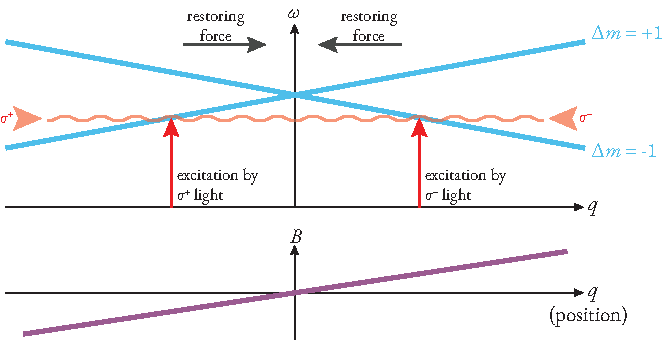
\includegraphics[scale=0.75]{\imagepath/detuning_and_selection_rules_schematic/detuning_and_selection_rules_schematic.pdf}
    \end{figure}

    \pause
    \begin{align*}
        \onslide<+->{
        F_\text{MOT} &= F_\text{scatter}^{\sigma^+}(\omega_\text{laser} - \omega_\text{transition}(q) - kv \cos \theta) - F_\text{scatter}^{\sigma^-}(\omega_\text{laser} - \omega_\text{transition}(q) + kv \cos \theta)} \\ \nonumber
        \onslide<+->{&\approx -2 \pdv{F_\text{scatter}}{\omega} k\cos \theta v + 2 \pdv{F_\text{scatter}}{\omega_0} \beta q  \equiv - (\alpha \cos \theta) v - \frac{\alpha \beta}{k} q}
    \end{align*}
\end{frame}

\begin{frame}
	\frametitle{Back to the MOT}
	\begin{figure}
        \centering
        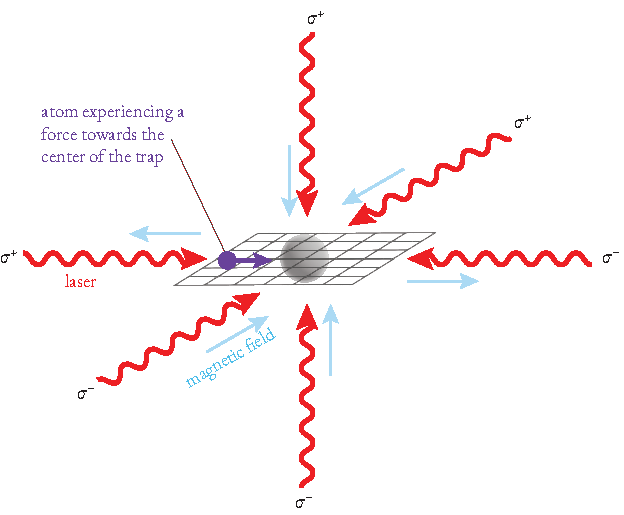
\includegraphics[height=0.8\textheight]{\imagepath/restoring_on_opposite_sides_schematic/restoring_on_opposite_sides_schematic.pdf}
    \end{figure}

    {\tiny Different helicities, same polarization! ($\sigma^+ \neq \Ket{\text{R}}$, $\sigma^- \neq \Ket{\text{L}}$)}
\end{frame}

\begin{frame}
    \frametitle{Transitions in a Lithium MOT}
    \begin{figure}
        \centering
        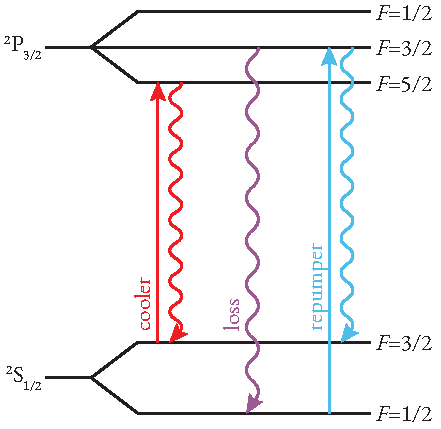
\includegraphics[scale=0.7]{\imagepath/cooler_repumper_in_alkali/cooler_repumper_in_alkali.pdf}
    \end{figure}
\end{frame}

\begin{frame}
    \frametitle{Capture velocity}
    Kinetic energy $\frac{1}{2}mv^2$ dissipated by force $\frac{\Gamma}{2} \hbar k$ along trajectory $2 r_\text{trap}$ in the MOT:
    \begin{align*}\label{eq:capture_velocity_high}
        v_\text{capture, max}^\text{high} = \sqrt{\frac{\hbar k \Gamma \cdot 2 r_\text{trap}}{m}} = \SI[]{90}{\meter\per\second}
    \end{align*}
\end{frame}

\begin{frame}
    \frametitle{Polarization}
    \begin{figure}
        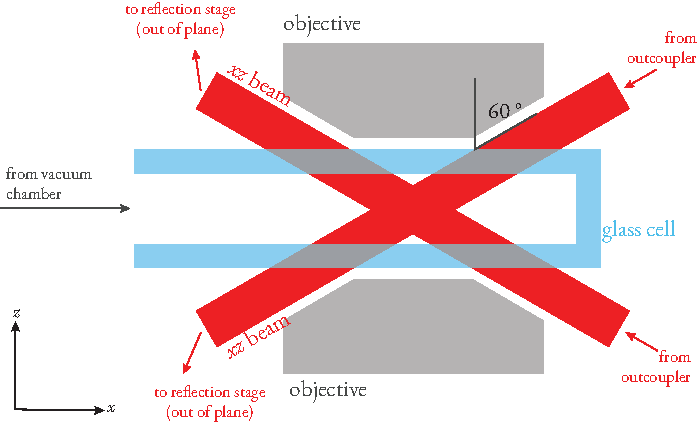
\includegraphics[scale=0.7]{\imagepath/glass_cell_sides_mot_beams/glass_cell_sides_mot_beams_1.pdf}
    \end{figure}
\end{frame}

\begin{frame}
    \frametitle{Polarization}
    \begin{columns}
        \begin{column}[]{0.45\textwidth}
            \centering
            First pass:
            \begin{figure}
                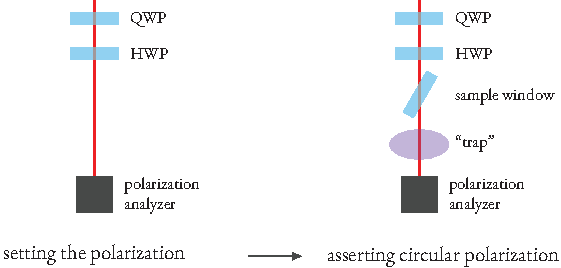
\includegraphics[scale=0.5]{\imagepath/first_pass_polarization_measurement_scheme/first_pass_polarization_measurement_scheme.pdf}
            \end{figure}
        \end{column}
        \begin{column}[]{0.55\textwidth}
            \centering
            Second pass:
            \begin{figure}
                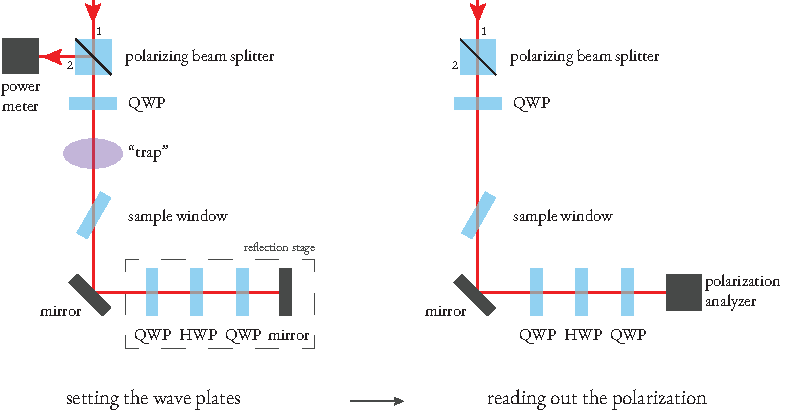
\includegraphics[scale=0.5]{\imagepath/second_pass_waveplate_adjustment_scheme/second_pass_waveplate_adjustment_scheme.pdf}
            \end{figure}
        \end{column}
    \end{columns}
\end{frame}

\renewcommand{\imagepath}{\textpath/40-coils/img}

\begin{frame}
    \begin{figure}
        \raggedleft
        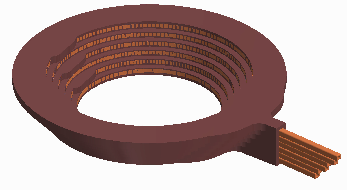
\includegraphics[]{\imagepath/single_coil_drawing/single_coil_drawing.pdf}
    \end{figure}
    \section{Feshbach Coils}
\end{frame}

\begin{frame}
    \frametitle{Constraints}

    \begin{columns}
        \begin{column}{0.4\textwidth}
            \begin{itemize}
                \item tight geometry
                \item field strength $\gg \SI[]{832}{\gauss}$
                \item water cooling
                \item curvature
            \end{itemize}
        \end{column}

        \begin{column}{0.55\textwidth}
            \begin{figure}
                \includegraphics[scale=0.7]{\imagepath/feshbach_coil_geometry_constraints/feshbach_coil_geometry_constraints.pdf}
            \end{figure}
        \end{column}
    \end{columns}
\end{frame}

\begin{frame}
    \frametitle{Tight Geometry}
    \begin{figure}
        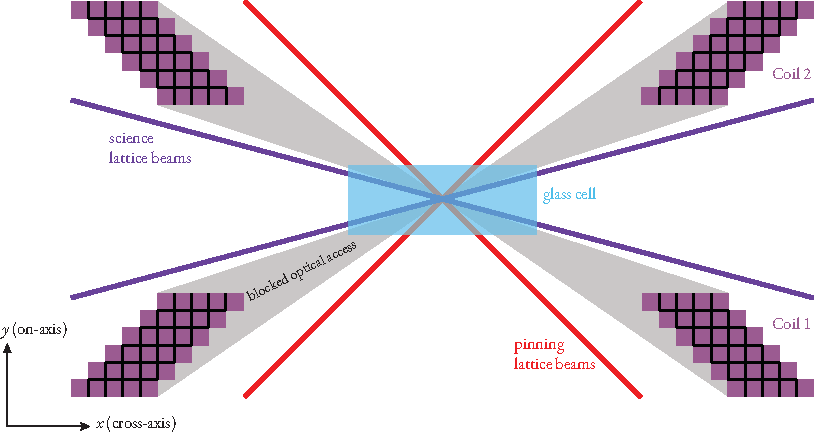
\includegraphics[scale=0.8]{\imagepath/parallelogram_cross_section/parallelogram_cross_section.pdf}
    \end{figure}
\end{frame}

\begin{frame}
    \frametitle{Field Strength}
    \begin{tikzpicture}
        \node (map) {\includegraphics[scale=0.7]{\imagepath/feshbach_field_map/feshbach_field_map.pdf}};
        \pause
        \node (overlay) at (map.south west) {\begin{pgfpicture}
            \pgftext{%% Creator: Matplotlib, PGF backend
%%
%% To include the figure in your LaTeX document, write
%%   \input{<filename>.pgf}
%%
%% Make sure the required packages are loaded in your preamble
%%   \usepackage{pgf}
%%
%% Also ensure that all the required font packages are loaded; for instance,
%% the lmodern package is sometimes necessary when using math font.
%%   \usepackage{lmodern}
%%
%% Figures using additional raster images can only be included by \input if
%% they are in the same directory as the main LaTeX file. For loading figures
%% from other directories you can use the `import` package
%%   \usepackage{import}
%%
%% and then include the figures with
%%   \import{<path to file>}{<filename>.pgf}
%%
%% Matplotlib used the following preamble
%%   \usepackage{fontspec}
%%   \setmainfont{DejaVuSerif.ttf}[Path=\detokenize{/home/max/.conda/envs/3d_mot/lib/python3.9/site-packages/matplotlib/mpl-data/fonts/ttf/}]
%%   \setsansfont{DejaVuSans.ttf}[Path=\detokenize{/home/max/.conda/envs/3d_mot/lib/python3.9/site-packages/matplotlib/mpl-data/fonts/ttf/}]
%%   \setmonofont{DejaVuSansMono.ttf}[Path=\detokenize{/home/max/.conda/envs/3d_mot/lib/python3.9/site-packages/matplotlib/mpl-data/fonts/ttf/}]
%%
\begingroup%
\makeatletter%
\begin{pgfpicture}%
\pgfpathrectangle{\pgfpointorigin}{\pgfqpoint{2.629021in}{1.496746in}}%
\pgfusepath{use as bounding box, clip}%
\begin{pgfscope}%
\pgfsetbuttcap%
\pgfsetmiterjoin%
\pgfsetlinewidth{0.000000pt}%
\definecolor{currentstroke}{rgb}{1.000000,1.000000,1.000000}%
\pgfsetstrokecolor{currentstroke}%
\pgfsetstrokeopacity{0.000000}%
\pgfsetdash{}{0pt}%
\pgfpathmoveto{\pgfqpoint{0.000000in}{0.000000in}}%
\pgfpathlineto{\pgfqpoint{2.629021in}{0.000000in}}%
\pgfpathlineto{\pgfqpoint{2.629021in}{1.496746in}}%
\pgfpathlineto{\pgfqpoint{0.000000in}{1.496746in}}%
\pgfpathlineto{\pgfqpoint{0.000000in}{0.000000in}}%
\pgfpathclose%
\pgfusepath{}%
\end{pgfscope}%
\begin{pgfscope}%
\pgfsetbuttcap%
\pgfsetmiterjoin%
\definecolor{currentfill}{rgb}{1.000000,1.000000,1.000000}%
\pgfsetfillcolor{currentfill}%
\pgfsetlinewidth{0.000000pt}%
\definecolor{currentstroke}{rgb}{0.000000,0.000000,0.000000}%
\pgfsetstrokecolor{currentstroke}%
\pgfsetstrokeopacity{0.000000}%
\pgfsetdash{}{0pt}%
\pgfpathmoveto{\pgfqpoint{0.695893in}{0.494721in}}%
\pgfpathlineto{\pgfqpoint{2.529021in}{0.494721in}}%
\pgfpathlineto{\pgfqpoint{2.529021in}{1.396746in}}%
\pgfpathlineto{\pgfqpoint{0.695893in}{1.396746in}}%
\pgfpathlineto{\pgfqpoint{0.695893in}{0.494721in}}%
\pgfpathclose%
\pgfusepath{fill}%
\end{pgfscope}%
\begin{pgfscope}%
\pgfpathrectangle{\pgfqpoint{0.695893in}{0.494721in}}{\pgfqpoint{1.833128in}{0.902025in}}%
\pgfusepath{clip}%
\pgfsetrectcap%
\pgfsetroundjoin%
\pgfsetlinewidth{0.803000pt}%
\definecolor{currentstroke}{rgb}{0.690196,0.690196,0.690196}%
\pgfsetstrokecolor{currentstroke}%
\pgfsetdash{}{0pt}%
\pgfpathmoveto{\pgfqpoint{1.110505in}{0.494721in}}%
\pgfpathlineto{\pgfqpoint{1.110505in}{1.396746in}}%
\pgfusepath{stroke}%
\end{pgfscope}%
\begin{pgfscope}%
\pgfsetbuttcap%
\pgfsetroundjoin%
\definecolor{currentfill}{rgb}{0.000000,0.000000,0.000000}%
\pgfsetfillcolor{currentfill}%
\pgfsetlinewidth{0.803000pt}%
\definecolor{currentstroke}{rgb}{0.000000,0.000000,0.000000}%
\pgfsetstrokecolor{currentstroke}%
\pgfsetdash{}{0pt}%
\pgfsys@defobject{currentmarker}{\pgfqpoint{0.000000in}{-0.048611in}}{\pgfqpoint{0.000000in}{0.000000in}}{%
\pgfpathmoveto{\pgfqpoint{0.000000in}{0.000000in}}%
\pgfpathlineto{\pgfqpoint{0.000000in}{-0.048611in}}%
\pgfusepath{stroke,fill}%
}%
\begin{pgfscope}%
\pgfsys@transformshift{1.110505in}{0.494721in}%
\pgfsys@useobject{currentmarker}{}%
\end{pgfscope}%
\end{pgfscope}%
\begin{pgfscope}%
\definecolor{textcolor}{rgb}{0.000000,0.000000,0.000000}%
\pgfsetstrokecolor{textcolor}%
\pgfsetfillcolor{textcolor}%
\pgftext[x=1.110505in,y=0.397499in,,top]{\color{textcolor}\rmfamily\fontsize{9.000000}{10.800000}\selectfont \ensuremath{-}100}%
\end{pgfscope}%
\begin{pgfscope}%
\pgfpathrectangle{\pgfqpoint{0.695893in}{0.494721in}}{\pgfqpoint{1.833128in}{0.902025in}}%
\pgfusepath{clip}%
\pgfsetrectcap%
\pgfsetroundjoin%
\pgfsetlinewidth{0.803000pt}%
\definecolor{currentstroke}{rgb}{0.690196,0.690196,0.690196}%
\pgfsetstrokecolor{currentstroke}%
\pgfsetdash{}{0pt}%
\pgfpathmoveto{\pgfqpoint{1.612457in}{0.494721in}}%
\pgfpathlineto{\pgfqpoint{1.612457in}{1.396746in}}%
\pgfusepath{stroke}%
\end{pgfscope}%
\begin{pgfscope}%
\pgfsetbuttcap%
\pgfsetroundjoin%
\definecolor{currentfill}{rgb}{0.000000,0.000000,0.000000}%
\pgfsetfillcolor{currentfill}%
\pgfsetlinewidth{0.803000pt}%
\definecolor{currentstroke}{rgb}{0.000000,0.000000,0.000000}%
\pgfsetstrokecolor{currentstroke}%
\pgfsetdash{}{0pt}%
\pgfsys@defobject{currentmarker}{\pgfqpoint{0.000000in}{-0.048611in}}{\pgfqpoint{0.000000in}{0.000000in}}{%
\pgfpathmoveto{\pgfqpoint{0.000000in}{0.000000in}}%
\pgfpathlineto{\pgfqpoint{0.000000in}{-0.048611in}}%
\pgfusepath{stroke,fill}%
}%
\begin{pgfscope}%
\pgfsys@transformshift{1.612457in}{0.494721in}%
\pgfsys@useobject{currentmarker}{}%
\end{pgfscope}%
\end{pgfscope}%
\begin{pgfscope}%
\definecolor{textcolor}{rgb}{0.000000,0.000000,0.000000}%
\pgfsetstrokecolor{textcolor}%
\pgfsetfillcolor{textcolor}%
\pgftext[x=1.612457in,y=0.397499in,,top]{\color{textcolor}\rmfamily\fontsize{9.000000}{10.800000}\selectfont 0}%
\end{pgfscope}%
\begin{pgfscope}%
\pgfpathrectangle{\pgfqpoint{0.695893in}{0.494721in}}{\pgfqpoint{1.833128in}{0.902025in}}%
\pgfusepath{clip}%
\pgfsetrectcap%
\pgfsetroundjoin%
\pgfsetlinewidth{0.803000pt}%
\definecolor{currentstroke}{rgb}{0.690196,0.690196,0.690196}%
\pgfsetstrokecolor{currentstroke}%
\pgfsetdash{}{0pt}%
\pgfpathmoveto{\pgfqpoint{2.114409in}{0.494721in}}%
\pgfpathlineto{\pgfqpoint{2.114409in}{1.396746in}}%
\pgfusepath{stroke}%
\end{pgfscope}%
\begin{pgfscope}%
\pgfsetbuttcap%
\pgfsetroundjoin%
\definecolor{currentfill}{rgb}{0.000000,0.000000,0.000000}%
\pgfsetfillcolor{currentfill}%
\pgfsetlinewidth{0.803000pt}%
\definecolor{currentstroke}{rgb}{0.000000,0.000000,0.000000}%
\pgfsetstrokecolor{currentstroke}%
\pgfsetdash{}{0pt}%
\pgfsys@defobject{currentmarker}{\pgfqpoint{0.000000in}{-0.048611in}}{\pgfqpoint{0.000000in}{0.000000in}}{%
\pgfpathmoveto{\pgfqpoint{0.000000in}{0.000000in}}%
\pgfpathlineto{\pgfqpoint{0.000000in}{-0.048611in}}%
\pgfusepath{stroke,fill}%
}%
\begin{pgfscope}%
\pgfsys@transformshift{2.114409in}{0.494721in}%
\pgfsys@useobject{currentmarker}{}%
\end{pgfscope}%
\end{pgfscope}%
\begin{pgfscope}%
\definecolor{textcolor}{rgb}{0.000000,0.000000,0.000000}%
\pgfsetstrokecolor{textcolor}%
\pgfsetfillcolor{textcolor}%
\pgftext[x=2.114409in,y=0.397499in,,top]{\color{textcolor}\rmfamily\fontsize{9.000000}{10.800000}\selectfont 100}%
\end{pgfscope}%
\begin{pgfscope}%
\definecolor{textcolor}{rgb}{0.000000,0.000000,0.000000}%
\pgfsetstrokecolor{textcolor}%
\pgfsetfillcolor{textcolor}%
\pgftext[x=1.612457in,y=0.220972in,,top]{\color{textcolor}\rmfamily\fontsize{9.000000}{10.800000}\selectfont position in mm}%
\end{pgfscope}%
\begin{pgfscope}%
\pgfpathrectangle{\pgfqpoint{0.695893in}{0.494721in}}{\pgfqpoint{1.833128in}{0.902025in}}%
\pgfusepath{clip}%
\pgfsetrectcap%
\pgfsetroundjoin%
\pgfsetlinewidth{0.803000pt}%
\definecolor{currentstroke}{rgb}{0.690196,0.690196,0.690196}%
\pgfsetstrokecolor{currentstroke}%
\pgfsetdash{}{0pt}%
\pgfpathmoveto{\pgfqpoint{0.695893in}{0.524344in}}%
\pgfpathlineto{\pgfqpoint{2.529021in}{0.524344in}}%
\pgfusepath{stroke}%
\end{pgfscope}%
\begin{pgfscope}%
\pgfsetbuttcap%
\pgfsetroundjoin%
\definecolor{currentfill}{rgb}{0.000000,0.000000,0.000000}%
\pgfsetfillcolor{currentfill}%
\pgfsetlinewidth{0.803000pt}%
\definecolor{currentstroke}{rgb}{0.000000,0.000000,0.000000}%
\pgfsetstrokecolor{currentstroke}%
\pgfsetdash{}{0pt}%
\pgfsys@defobject{currentmarker}{\pgfqpoint{-0.048611in}{0.000000in}}{\pgfqpoint{-0.000000in}{0.000000in}}{%
\pgfpathmoveto{\pgfqpoint{-0.000000in}{0.000000in}}%
\pgfpathlineto{\pgfqpoint{-0.048611in}{0.000000in}}%
\pgfusepath{stroke,fill}%
}%
\begin{pgfscope}%
\pgfsys@transformshift{0.695893in}{0.524344in}%
\pgfsys@useobject{currentmarker}{}%
\end{pgfscope}%
\end{pgfscope}%
\begin{pgfscope}%
\definecolor{textcolor}{rgb}{0.000000,0.000000,0.000000}%
\pgfsetstrokecolor{textcolor}%
\pgfsetfillcolor{textcolor}%
\pgftext[x=0.519142in, y=0.476859in, left, base]{\color{textcolor}\rmfamily\fontsize{9.000000}{10.800000}\selectfont 0}%
\end{pgfscope}%
\begin{pgfscope}%
\pgfpathrectangle{\pgfqpoint{0.695893in}{0.494721in}}{\pgfqpoint{1.833128in}{0.902025in}}%
\pgfusepath{clip}%
\pgfsetrectcap%
\pgfsetroundjoin%
\pgfsetlinewidth{0.803000pt}%
\definecolor{currentstroke}{rgb}{0.690196,0.690196,0.690196}%
\pgfsetstrokecolor{currentstroke}%
\pgfsetdash{}{0pt}%
\pgfpathmoveto{\pgfqpoint{0.695893in}{0.841958in}}%
\pgfpathlineto{\pgfqpoint{2.529021in}{0.841958in}}%
\pgfusepath{stroke}%
\end{pgfscope}%
\begin{pgfscope}%
\pgfsetbuttcap%
\pgfsetroundjoin%
\definecolor{currentfill}{rgb}{0.000000,0.000000,0.000000}%
\pgfsetfillcolor{currentfill}%
\pgfsetlinewidth{0.803000pt}%
\definecolor{currentstroke}{rgb}{0.000000,0.000000,0.000000}%
\pgfsetstrokecolor{currentstroke}%
\pgfsetdash{}{0pt}%
\pgfsys@defobject{currentmarker}{\pgfqpoint{-0.048611in}{0.000000in}}{\pgfqpoint{-0.000000in}{0.000000in}}{%
\pgfpathmoveto{\pgfqpoint{-0.000000in}{0.000000in}}%
\pgfpathlineto{\pgfqpoint{-0.048611in}{0.000000in}}%
\pgfusepath{stroke,fill}%
}%
\begin{pgfscope}%
\pgfsys@transformshift{0.695893in}{0.841958in}%
\pgfsys@useobject{currentmarker}{}%
\end{pgfscope}%
\end{pgfscope}%
\begin{pgfscope}%
\definecolor{textcolor}{rgb}{0.000000,0.000000,0.000000}%
\pgfsetstrokecolor{textcolor}%
\pgfsetfillcolor{textcolor}%
\pgftext[x=0.360084in, y=0.794473in, left, base]{\color{textcolor}\rmfamily\fontsize{9.000000}{10.800000}\selectfont 500}%
\end{pgfscope}%
\begin{pgfscope}%
\pgfpathrectangle{\pgfqpoint{0.695893in}{0.494721in}}{\pgfqpoint{1.833128in}{0.902025in}}%
\pgfusepath{clip}%
\pgfsetrectcap%
\pgfsetroundjoin%
\pgfsetlinewidth{0.803000pt}%
\definecolor{currentstroke}{rgb}{0.690196,0.690196,0.690196}%
\pgfsetstrokecolor{currentstroke}%
\pgfsetdash{}{0pt}%
\pgfpathmoveto{\pgfqpoint{0.695893in}{1.159572in}}%
\pgfpathlineto{\pgfqpoint{2.529021in}{1.159572in}}%
\pgfusepath{stroke}%
\end{pgfscope}%
\begin{pgfscope}%
\pgfsetbuttcap%
\pgfsetroundjoin%
\definecolor{currentfill}{rgb}{0.000000,0.000000,0.000000}%
\pgfsetfillcolor{currentfill}%
\pgfsetlinewidth{0.803000pt}%
\definecolor{currentstroke}{rgb}{0.000000,0.000000,0.000000}%
\pgfsetstrokecolor{currentstroke}%
\pgfsetdash{}{0pt}%
\pgfsys@defobject{currentmarker}{\pgfqpoint{-0.048611in}{0.000000in}}{\pgfqpoint{-0.000000in}{0.000000in}}{%
\pgfpathmoveto{\pgfqpoint{-0.000000in}{0.000000in}}%
\pgfpathlineto{\pgfqpoint{-0.048611in}{0.000000in}}%
\pgfusepath{stroke,fill}%
}%
\begin{pgfscope}%
\pgfsys@transformshift{0.695893in}{1.159572in}%
\pgfsys@useobject{currentmarker}{}%
\end{pgfscope}%
\end{pgfscope}%
\begin{pgfscope}%
\definecolor{textcolor}{rgb}{0.000000,0.000000,0.000000}%
\pgfsetstrokecolor{textcolor}%
\pgfsetfillcolor{textcolor}%
\pgftext[x=0.280556in, y=1.112087in, left, base]{\color{textcolor}\rmfamily\fontsize{9.000000}{10.800000}\selectfont 1000}%
\end{pgfscope}%
\begin{pgfscope}%
\definecolor{textcolor}{rgb}{0.000000,0.000000,0.000000}%
\pgfsetstrokecolor{textcolor}%
\pgfsetfillcolor{textcolor}%
\pgftext[x=0.225000in,y=0.945734in,,bottom,rotate=90.000000]{\color{textcolor}\rmfamily\fontsize{9.000000}{10.800000}\selectfont \(\displaystyle |B|\) in G}%
\end{pgfscope}%
\begin{pgfscope}%
\pgfpathrectangle{\pgfqpoint{0.695893in}{0.494721in}}{\pgfqpoint{1.833128in}{0.902025in}}%
\pgfusepath{clip}%
\pgfsetrectcap%
\pgfsetroundjoin%
\pgfsetlinewidth{1.505625pt}%
\definecolor{currentstroke}{rgb}{1.000000,0.000000,0.000000}%
\pgfsetstrokecolor{currentstroke}%
\pgfsetdash{}{0pt}%
\pgfpathmoveto{\pgfqpoint{0.779217in}{0.654694in}}%
\pgfpathlineto{\pgfqpoint{0.796050in}{0.661669in}}%
\pgfpathlineto{\pgfqpoint{0.812883in}{0.669094in}}%
\pgfpathlineto{\pgfqpoint{0.829716in}{0.676997in}}%
\pgfpathlineto{\pgfqpoint{0.846550in}{0.685409in}}%
\pgfpathlineto{\pgfqpoint{0.863383in}{0.694365in}}%
\pgfpathlineto{\pgfqpoint{0.880216in}{0.703899in}}%
\pgfpathlineto{\pgfqpoint{0.897049in}{0.714044in}}%
\pgfpathlineto{\pgfqpoint{0.913882in}{0.724839in}}%
\pgfpathlineto{\pgfqpoint{0.930715in}{0.736319in}}%
\pgfpathlineto{\pgfqpoint{0.947548in}{0.748521in}}%
\pgfpathlineto{\pgfqpoint{0.964381in}{0.761483in}}%
\pgfpathlineto{\pgfqpoint{0.981215in}{0.775239in}}%
\pgfpathlineto{\pgfqpoint{0.998048in}{0.789823in}}%
\pgfpathlineto{\pgfqpoint{1.014881in}{0.805267in}}%
\pgfpathlineto{\pgfqpoint{1.031714in}{0.821596in}}%
\pgfpathlineto{\pgfqpoint{1.048547in}{0.838833in}}%
\pgfpathlineto{\pgfqpoint{1.065380in}{0.856993in}}%
\pgfpathlineto{\pgfqpoint{1.082213in}{0.876081in}}%
\pgfpathlineto{\pgfqpoint{1.099046in}{0.896092in}}%
\pgfpathlineto{\pgfqpoint{1.115880in}{0.917011in}}%
\pgfpathlineto{\pgfqpoint{1.132713in}{0.938804in}}%
\pgfpathlineto{\pgfqpoint{1.149546in}{0.961424in}}%
\pgfpathlineto{\pgfqpoint{1.166379in}{0.984801in}}%
\pgfpathlineto{\pgfqpoint{1.183212in}{1.008845in}}%
\pgfpathlineto{\pgfqpoint{1.200045in}{1.033444in}}%
\pgfpathlineto{\pgfqpoint{1.216878in}{1.058459in}}%
\pgfpathlineto{\pgfqpoint{1.233712in}{1.083727in}}%
\pgfpathlineto{\pgfqpoint{1.250545in}{1.109059in}}%
\pgfpathlineto{\pgfqpoint{1.267378in}{1.134243in}}%
\pgfpathlineto{\pgfqpoint{1.284211in}{1.159046in}}%
\pgfpathlineto{\pgfqpoint{1.301044in}{1.183219in}}%
\pgfpathlineto{\pgfqpoint{1.317877in}{1.206502in}}%
\pgfpathlineto{\pgfqpoint{1.334710in}{1.228635in}}%
\pgfpathlineto{\pgfqpoint{1.351543in}{1.249366in}}%
\pgfpathlineto{\pgfqpoint{1.368377in}{1.268463in}}%
\pgfpathlineto{\pgfqpoint{1.385210in}{1.285729in}}%
\pgfpathlineto{\pgfqpoint{1.402043in}{1.301011in}}%
\pgfpathlineto{\pgfqpoint{1.418876in}{1.314213in}}%
\pgfpathlineto{\pgfqpoint{1.435709in}{1.325308in}}%
\pgfpathlineto{\pgfqpoint{1.452542in}{1.334337in}}%
\pgfpathlineto{\pgfqpoint{1.469375in}{1.341415in}}%
\pgfpathlineto{\pgfqpoint{1.486208in}{1.346719in}}%
\pgfpathlineto{\pgfqpoint{1.503042in}{1.350482in}}%
\pgfpathlineto{\pgfqpoint{1.519875in}{1.352973in}}%
\pgfpathlineto{\pgfqpoint{1.536708in}{1.354477in}}%
\pgfpathlineto{\pgfqpoint{1.553541in}{1.355275in}}%
\pgfpathlineto{\pgfqpoint{1.570374in}{1.355623in}}%
\pgfpathlineto{\pgfqpoint{1.587207in}{1.355730in}}%
\pgfpathlineto{\pgfqpoint{1.604040in}{1.355745in}}%
\pgfpathlineto{\pgfqpoint{1.620873in}{1.355745in}}%
\pgfpathlineto{\pgfqpoint{1.637707in}{1.355730in}}%
\pgfpathlineto{\pgfqpoint{1.654540in}{1.355623in}}%
\pgfpathlineto{\pgfqpoint{1.671373in}{1.355275in}}%
\pgfpathlineto{\pgfqpoint{1.688206in}{1.354477in}}%
\pgfpathlineto{\pgfqpoint{1.705039in}{1.352973in}}%
\pgfpathlineto{\pgfqpoint{1.721872in}{1.350482in}}%
\pgfpathlineto{\pgfqpoint{1.738705in}{1.346719in}}%
\pgfpathlineto{\pgfqpoint{1.755539in}{1.341415in}}%
\pgfpathlineto{\pgfqpoint{1.772372in}{1.334337in}}%
\pgfpathlineto{\pgfqpoint{1.789205in}{1.325308in}}%
\pgfpathlineto{\pgfqpoint{1.806038in}{1.314213in}}%
\pgfpathlineto{\pgfqpoint{1.822871in}{1.301011in}}%
\pgfpathlineto{\pgfqpoint{1.839704in}{1.285729in}}%
\pgfpathlineto{\pgfqpoint{1.856537in}{1.268463in}}%
\pgfpathlineto{\pgfqpoint{1.873370in}{1.249366in}}%
\pgfpathlineto{\pgfqpoint{1.890204in}{1.228635in}}%
\pgfpathlineto{\pgfqpoint{1.907037in}{1.206502in}}%
\pgfpathlineto{\pgfqpoint{1.923870in}{1.183219in}}%
\pgfpathlineto{\pgfqpoint{1.940703in}{1.159046in}}%
\pgfpathlineto{\pgfqpoint{1.957536in}{1.134243in}}%
\pgfpathlineto{\pgfqpoint{1.974369in}{1.109059in}}%
\pgfpathlineto{\pgfqpoint{1.991202in}{1.083727in}}%
\pgfpathlineto{\pgfqpoint{2.008035in}{1.058459in}}%
\pgfpathlineto{\pgfqpoint{2.024869in}{1.033444in}}%
\pgfpathlineto{\pgfqpoint{2.041702in}{1.008845in}}%
\pgfpathlineto{\pgfqpoint{2.058535in}{0.984801in}}%
\pgfpathlineto{\pgfqpoint{2.075368in}{0.961424in}}%
\pgfpathlineto{\pgfqpoint{2.092201in}{0.938804in}}%
\pgfpathlineto{\pgfqpoint{2.109034in}{0.917011in}}%
\pgfpathlineto{\pgfqpoint{2.125867in}{0.896092in}}%
\pgfpathlineto{\pgfqpoint{2.142700in}{0.876081in}}%
\pgfpathlineto{\pgfqpoint{2.159534in}{0.856993in}}%
\pgfpathlineto{\pgfqpoint{2.176367in}{0.838833in}}%
\pgfpathlineto{\pgfqpoint{2.193200in}{0.821596in}}%
\pgfpathlineto{\pgfqpoint{2.210033in}{0.805267in}}%
\pgfpathlineto{\pgfqpoint{2.226866in}{0.789823in}}%
\pgfpathlineto{\pgfqpoint{2.243699in}{0.775239in}}%
\pgfpathlineto{\pgfqpoint{2.260532in}{0.761483in}}%
\pgfpathlineto{\pgfqpoint{2.277366in}{0.748521in}}%
\pgfpathlineto{\pgfqpoint{2.294199in}{0.736319in}}%
\pgfpathlineto{\pgfqpoint{2.311032in}{0.724839in}}%
\pgfpathlineto{\pgfqpoint{2.327865in}{0.714044in}}%
\pgfpathlineto{\pgfqpoint{2.344698in}{0.703899in}}%
\pgfpathlineto{\pgfqpoint{2.361531in}{0.694365in}}%
\pgfpathlineto{\pgfqpoint{2.378364in}{0.685409in}}%
\pgfpathlineto{\pgfqpoint{2.395197in}{0.676997in}}%
\pgfpathlineto{\pgfqpoint{2.412031in}{0.669094in}}%
\pgfpathlineto{\pgfqpoint{2.428864in}{0.661669in}}%
\pgfpathlineto{\pgfqpoint{2.445697in}{0.654694in}}%
\pgfusepath{stroke}%
\end{pgfscope}%
\begin{pgfscope}%
\pgfpathrectangle{\pgfqpoint{0.695893in}{0.494721in}}{\pgfqpoint{1.833128in}{0.902025in}}%
\pgfusepath{clip}%
\pgfsetrectcap%
\pgfsetroundjoin%
\pgfsetlinewidth{1.505625pt}%
\definecolor{currentstroke}{rgb}{0.313725,0.741176,0.913725}%
\pgfsetstrokecolor{currentstroke}%
\pgfsetdash{}{0pt}%
\pgfpathmoveto{\pgfqpoint{0.779217in}{0.580467in}}%
\pgfpathlineto{\pgfqpoint{0.796050in}{0.582467in}}%
\pgfpathlineto{\pgfqpoint{0.812883in}{0.584407in}}%
\pgfpathlineto{\pgfqpoint{0.829716in}{0.586243in}}%
\pgfpathlineto{\pgfqpoint{0.846550in}{0.587920in}}%
\pgfpathlineto{\pgfqpoint{0.863383in}{0.589369in}}%
\pgfpathlineto{\pgfqpoint{0.880216in}{0.590503in}}%
\pgfpathlineto{\pgfqpoint{0.897049in}{0.591219in}}%
\pgfpathlineto{\pgfqpoint{0.913882in}{0.591389in}}%
\pgfpathlineto{\pgfqpoint{0.930715in}{0.590858in}}%
\pgfpathlineto{\pgfqpoint{0.947548in}{0.589445in}}%
\pgfpathlineto{\pgfqpoint{0.964381in}{0.586933in}}%
\pgfpathlineto{\pgfqpoint{0.981215in}{0.583074in}}%
\pgfpathlineto{\pgfqpoint{0.998048in}{0.577586in}}%
\pgfpathlineto{\pgfqpoint{1.014881in}{0.570162in}}%
\pgfpathlineto{\pgfqpoint{1.031714in}{0.560502in}}%
\pgfpathlineto{\pgfqpoint{1.048547in}{0.548469in}}%
\pgfpathlineto{\pgfqpoint{1.065380in}{0.535722in}}%
\pgfpathlineto{\pgfqpoint{1.082213in}{0.540756in}}%
\pgfpathlineto{\pgfqpoint{1.099046in}{0.562647in}}%
\pgfpathlineto{\pgfqpoint{1.115880in}{0.590414in}}%
\pgfpathlineto{\pgfqpoint{1.132713in}{0.623359in}}%
\pgfpathlineto{\pgfqpoint{1.149546in}{0.661525in}}%
\pgfpathlineto{\pgfqpoint{1.166379in}{0.704873in}}%
\pgfpathlineto{\pgfqpoint{1.183212in}{0.753117in}}%
\pgfpathlineto{\pgfqpoint{1.200045in}{0.805634in}}%
\pgfpathlineto{\pgfqpoint{1.216878in}{0.861434in}}%
\pgfpathlineto{\pgfqpoint{1.233712in}{0.919190in}}%
\pgfpathlineto{\pgfqpoint{1.250545in}{0.977339in}}%
\pgfpathlineto{\pgfqpoint{1.267378in}{1.034225in}}%
\pgfpathlineto{\pgfqpoint{1.284211in}{1.088252in}}%
\pgfpathlineto{\pgfqpoint{1.301044in}{1.138032in}}%
\pgfpathlineto{\pgfqpoint{1.317877in}{1.182503in}}%
\pgfpathlineto{\pgfqpoint{1.334710in}{1.221015in}}%
\pgfpathlineto{\pgfqpoint{1.351543in}{1.253360in}}%
\pgfpathlineto{\pgfqpoint{1.368377in}{1.279733in}}%
\pgfpathlineto{\pgfqpoint{1.385210in}{1.300643in}}%
\pgfpathlineto{\pgfqpoint{1.402043in}{1.316789in}}%
\pgfpathlineto{\pgfqpoint{1.418876in}{1.328944in}}%
\pgfpathlineto{\pgfqpoint{1.435709in}{1.337868in}}%
\pgfpathlineto{\pgfqpoint{1.452542in}{1.344245in}}%
\pgfpathlineto{\pgfqpoint{1.469375in}{1.348669in}}%
\pgfpathlineto{\pgfqpoint{1.486208in}{1.351629in}}%
\pgfpathlineto{\pgfqpoint{1.503042in}{1.353522in}}%
\pgfpathlineto{\pgfqpoint{1.519875in}{1.354661in}}%
\pgfpathlineto{\pgfqpoint{1.536708in}{1.355291in}}%
\pgfpathlineto{\pgfqpoint{1.553541in}{1.355597in}}%
\pgfpathlineto{\pgfqpoint{1.570374in}{1.355716in}}%
\pgfpathlineto{\pgfqpoint{1.587207in}{1.355745in}}%
\pgfpathlineto{\pgfqpoint{1.604040in}{1.355745in}}%
\pgfpathlineto{\pgfqpoint{1.620873in}{1.355745in}}%
\pgfpathlineto{\pgfqpoint{1.637707in}{1.355745in}}%
\pgfpathlineto{\pgfqpoint{1.654540in}{1.355716in}}%
\pgfpathlineto{\pgfqpoint{1.671373in}{1.355597in}}%
\pgfpathlineto{\pgfqpoint{1.688206in}{1.355291in}}%
\pgfpathlineto{\pgfqpoint{1.705039in}{1.354661in}}%
\pgfpathlineto{\pgfqpoint{1.721872in}{1.353522in}}%
\pgfpathlineto{\pgfqpoint{1.738705in}{1.351629in}}%
\pgfpathlineto{\pgfqpoint{1.755539in}{1.348669in}}%
\pgfpathlineto{\pgfqpoint{1.772372in}{1.344245in}}%
\pgfpathlineto{\pgfqpoint{1.789205in}{1.337868in}}%
\pgfpathlineto{\pgfqpoint{1.806038in}{1.328944in}}%
\pgfpathlineto{\pgfqpoint{1.822871in}{1.316789in}}%
\pgfpathlineto{\pgfqpoint{1.839704in}{1.300643in}}%
\pgfpathlineto{\pgfqpoint{1.856537in}{1.279733in}}%
\pgfpathlineto{\pgfqpoint{1.873370in}{1.253360in}}%
\pgfpathlineto{\pgfqpoint{1.890204in}{1.221015in}}%
\pgfpathlineto{\pgfqpoint{1.907037in}{1.182503in}}%
\pgfpathlineto{\pgfqpoint{1.923870in}{1.138032in}}%
\pgfpathlineto{\pgfqpoint{1.940703in}{1.088252in}}%
\pgfpathlineto{\pgfqpoint{1.957536in}{1.034225in}}%
\pgfpathlineto{\pgfqpoint{1.974369in}{0.977339in}}%
\pgfpathlineto{\pgfqpoint{1.991202in}{0.919190in}}%
\pgfpathlineto{\pgfqpoint{2.008035in}{0.861434in}}%
\pgfpathlineto{\pgfqpoint{2.024869in}{0.805634in}}%
\pgfpathlineto{\pgfqpoint{2.041702in}{0.753117in}}%
\pgfpathlineto{\pgfqpoint{2.058535in}{0.704873in}}%
\pgfpathlineto{\pgfqpoint{2.075368in}{0.661525in}}%
\pgfpathlineto{\pgfqpoint{2.092201in}{0.623359in}}%
\pgfpathlineto{\pgfqpoint{2.109034in}{0.590414in}}%
\pgfpathlineto{\pgfqpoint{2.125867in}{0.562647in}}%
\pgfpathlineto{\pgfqpoint{2.142700in}{0.540756in}}%
\pgfpathlineto{\pgfqpoint{2.159534in}{0.535722in}}%
\pgfpathlineto{\pgfqpoint{2.176367in}{0.548469in}}%
\pgfpathlineto{\pgfqpoint{2.193200in}{0.560502in}}%
\pgfpathlineto{\pgfqpoint{2.210033in}{0.570162in}}%
\pgfpathlineto{\pgfqpoint{2.226866in}{0.577586in}}%
\pgfpathlineto{\pgfqpoint{2.243699in}{0.583074in}}%
\pgfpathlineto{\pgfqpoint{2.260532in}{0.586933in}}%
\pgfpathlineto{\pgfqpoint{2.277366in}{0.589445in}}%
\pgfpathlineto{\pgfqpoint{2.294199in}{0.590858in}}%
\pgfpathlineto{\pgfqpoint{2.311032in}{0.591389in}}%
\pgfpathlineto{\pgfqpoint{2.327865in}{0.591219in}}%
\pgfpathlineto{\pgfqpoint{2.344698in}{0.590503in}}%
\pgfpathlineto{\pgfqpoint{2.361531in}{0.589369in}}%
\pgfpathlineto{\pgfqpoint{2.378364in}{0.587920in}}%
\pgfpathlineto{\pgfqpoint{2.395197in}{0.586243in}}%
\pgfpathlineto{\pgfqpoint{2.412031in}{0.584407in}}%
\pgfpathlineto{\pgfqpoint{2.428864in}{0.582467in}}%
\pgfpathlineto{\pgfqpoint{2.445697in}{0.580467in}}%
\pgfusepath{stroke}%
\end{pgfscope}%
\begin{pgfscope}%
\pgfsetrectcap%
\pgfsetmiterjoin%
\pgfsetlinewidth{0.803000pt}%
\definecolor{currentstroke}{rgb}{0.000000,0.000000,0.000000}%
\pgfsetstrokecolor{currentstroke}%
\pgfsetdash{}{0pt}%
\pgfpathmoveto{\pgfqpoint{0.695893in}{0.494721in}}%
\pgfpathlineto{\pgfqpoint{0.695893in}{1.396746in}}%
\pgfusepath{stroke}%
\end{pgfscope}%
\begin{pgfscope}%
\pgfsetrectcap%
\pgfsetmiterjoin%
\pgfsetlinewidth{0.803000pt}%
\definecolor{currentstroke}{rgb}{0.000000,0.000000,0.000000}%
\pgfsetstrokecolor{currentstroke}%
\pgfsetdash{}{0pt}%
\pgfpathmoveto{\pgfqpoint{2.529021in}{0.494721in}}%
\pgfpathlineto{\pgfqpoint{2.529021in}{1.396746in}}%
\pgfusepath{stroke}%
\end{pgfscope}%
\begin{pgfscope}%
\pgfsetrectcap%
\pgfsetmiterjoin%
\pgfsetlinewidth{0.803000pt}%
\definecolor{currentstroke}{rgb}{0.000000,0.000000,0.000000}%
\pgfsetstrokecolor{currentstroke}%
\pgfsetdash{}{0pt}%
\pgfpathmoveto{\pgfqpoint{0.695893in}{0.494721in}}%
\pgfpathlineto{\pgfqpoint{2.529021in}{0.494721in}}%
\pgfusepath{stroke}%
\end{pgfscope}%
\begin{pgfscope}%
\pgfsetrectcap%
\pgfsetmiterjoin%
\pgfsetlinewidth{0.803000pt}%
\definecolor{currentstroke}{rgb}{0.000000,0.000000,0.000000}%
\pgfsetstrokecolor{currentstroke}%
\pgfsetdash{}{0pt}%
\pgfpathmoveto{\pgfqpoint{0.695893in}{1.396746in}}%
\pgfpathlineto{\pgfqpoint{2.529021in}{1.396746in}}%
\pgfusepath{stroke}%
\end{pgfscope}%
\begin{pgfscope}%
\pgfsetbuttcap%
\pgfsetmiterjoin%
\definecolor{currentfill}{rgb}{1.000000,1.000000,1.000000}%
\pgfsetfillcolor{currentfill}%
\pgfsetfillopacity{0.800000}%
\pgfsetlinewidth{1.003750pt}%
\definecolor{currentstroke}{rgb}{0.800000,0.800000,0.800000}%
\pgfsetstrokecolor{currentstroke}%
\pgfsetstrokeopacity{0.800000}%
\pgfsetdash{}{0pt}%
\pgfpathmoveto{\pgfqpoint{1.270892in}{0.536388in}}%
\pgfpathlineto{\pgfqpoint{1.954022in}{0.536388in}}%
\pgfpathquadraticcurveto{\pgfqpoint{1.970689in}{0.536388in}}{\pgfqpoint{1.970689in}{0.553054in}}%
\pgfpathlineto{\pgfqpoint{1.970689in}{0.789349in}}%
\pgfpathquadraticcurveto{\pgfqpoint{1.970689in}{0.806016in}}{\pgfqpoint{1.954022in}{0.806016in}}%
\pgfpathlineto{\pgfqpoint{1.270892in}{0.806016in}}%
\pgfpathquadraticcurveto{\pgfqpoint{1.254225in}{0.806016in}}{\pgfqpoint{1.254225in}{0.789349in}}%
\pgfpathlineto{\pgfqpoint{1.254225in}{0.553054in}}%
\pgfpathquadraticcurveto{\pgfqpoint{1.254225in}{0.536388in}}{\pgfqpoint{1.270892in}{0.536388in}}%
\pgfpathlineto{\pgfqpoint{1.270892in}{0.536388in}}%
\pgfpathclose%
\pgfusepath{stroke,fill}%
\end{pgfscope}%
\begin{pgfscope}%
\pgfsetrectcap%
\pgfsetroundjoin%
\pgfsetlinewidth{1.505625pt}%
\definecolor{currentstroke}{rgb}{1.000000,0.000000,0.000000}%
\pgfsetstrokecolor{currentstroke}%
\pgfsetdash{}{0pt}%
\pgfpathmoveto{\pgfqpoint{1.287559in}{0.738536in}}%
\pgfpathlineto{\pgfqpoint{1.370892in}{0.738536in}}%
\pgfpathlineto{\pgfqpoint{1.454225in}{0.738536in}}%
\pgfusepath{stroke}%
\end{pgfscope}%
\begin{pgfscope}%
\definecolor{textcolor}{rgb}{0.000000,0.000000,0.000000}%
\pgfsetstrokecolor{textcolor}%
\pgfsetfillcolor{textcolor}%
\pgftext[x=1.520892in,y=0.709369in,left,base]{\color{textcolor}\rmfamily\fontsize{6.000000}{7.200000}\selectfont on-axis}%
\end{pgfscope}%
\begin{pgfscope}%
\pgfsetrectcap%
\pgfsetroundjoin%
\pgfsetlinewidth{1.505625pt}%
\definecolor{currentstroke}{rgb}{0.313725,0.741176,0.913725}%
\pgfsetstrokecolor{currentstroke}%
\pgfsetdash{}{0pt}%
\pgfpathmoveto{\pgfqpoint{1.287559in}{0.616221in}}%
\pgfpathlineto{\pgfqpoint{1.370892in}{0.616221in}}%
\pgfpathlineto{\pgfqpoint{1.454225in}{0.616221in}}%
\pgfusepath{stroke}%
\end{pgfscope}%
\begin{pgfscope}%
\definecolor{textcolor}{rgb}{0.000000,0.000000,0.000000}%
\pgfsetstrokecolor{textcolor}%
\pgfsetfillcolor{textcolor}%
\pgftext[x=1.520892in,y=0.587055in,left,base]{\color{textcolor}\rmfamily\fontsize{6.000000}{7.200000}\selectfont cross-axis}%
\end{pgfscope}%
\end{pgfpicture}%
\makeatother%
\endgroup%
}
        \end{pgfpicture}};
    \end{tikzpicture}
\end{frame}

\renewcommand{\imagepath}{\textpath/90-appendix/img}
\setbeamercovered{transparent}
\begin{frame}
    \frametitle{Field Strength :: Rules of Thumb}
    \vspace{0.5cm}

    \begin{columns}
        \begin{column}{0.38\textwidth}
            \centering
            \onslide<1>{
                \textbf{Homogeneous field:}
                \begin{align*}
                    B(r, I) \approx \left. \frac{I}{\SI{1}{\ampere}} \middle/ \frac{r}{\SI{1}{\centi\meter}} ~ \cdot ~\SI{1}{\gauss}\right.
                \end{align*}

                ``$
                    \SI{1}{\gauss} ~~ \text{per} ~~ \frac{\si{\ampere} ~~ \text{of current}}{\si{\centi\meter} ~~ \text{of radius}}
                $''
            }

            \vspace{1cm}

            \onslide<2>{
                \centering
                \textbf{Gradient field:}
                    \begin{align*}
                        \pdv{B(r, I)}{x_\text{on-axis}} \approx \left. \frac{I}{\SI{1}{\ampere}} \middle/ \left(\frac{r}{\SI{1}{\centi\meter}}\right)^2 ~\cdot~ \SI{1}{\gauss\per\centi\meter} \right.
                    \end{align*}
            }
        \end{column}

        \begin{column}{0.6\textwidth}
            \only<1>{
                \begin{figure}
                    \centering
                    \scalebox{0.55}{
                        \begin{pgfpicture}
                            \pgftext{%% Creator: Matplotlib, PGF backend
%%
%% To include the figure in your LaTeX document, write
%%   \input{<filename>.pgf}
%%
%% Make sure the required packages are loaded in your preamble
%%   \usepackage{pgf}
%%
%% Also ensure that all the required font packages are loaded; for instance,
%% the lmodern package is sometimes necessary when using math font.
%%   \usepackage{lmodern}
%%
%% Figures using additional raster images can only be included by \input if
%% they are in the same directory as the main LaTeX file. For loading figures
%% from other directories you can use the `import` package
%%   \usepackage{import}
%%
%% and then include the figures with
%%   \import{<path to file>}{<filename>.pgf}
%%
%% Matplotlib used the following preamble
%%   \usepackage{fontspec}
%%   \setmainfont{DejaVuSerif.ttf}[Path=\detokenize{/home/max/.conda/envs/3d_mot/lib/python3.9/site-packages/matplotlib/mpl-data/fonts/ttf/}]
%%   \setsansfont{DejaVuSans.ttf}[Path=\detokenize{/home/max/.conda/envs/3d_mot/lib/python3.9/site-packages/matplotlib/mpl-data/fonts/ttf/}]
%%   \setmonofont{DejaVuSansMono.ttf}[Path=\detokenize{/home/max/.conda/envs/3d_mot/lib/python3.9/site-packages/matplotlib/mpl-data/fonts/ttf/}]
%%
\begingroup%
\makeatletter%
\begin{pgfpicture}%
\pgfpathrectangle{\pgfpointorigin}{\pgfqpoint{2.463516in}{1.635075in}}%
\pgfusepath{use as bounding box, clip}%
\begin{pgfscope}%
\pgfsetbuttcap%
\pgfsetmiterjoin%
\pgfsetlinewidth{0.000000pt}%
\definecolor{currentstroke}{rgb}{1.000000,1.000000,1.000000}%
\pgfsetstrokecolor{currentstroke}%
\pgfsetstrokeopacity{0.000000}%
\pgfsetdash{}{0pt}%
\pgfpathmoveto{\pgfqpoint{0.000000in}{0.000000in}}%
\pgfpathlineto{\pgfqpoint{2.463516in}{0.000000in}}%
\pgfpathlineto{\pgfqpoint{2.463516in}{1.635075in}}%
\pgfpathlineto{\pgfqpoint{0.000000in}{1.635075in}}%
\pgfpathlineto{\pgfqpoint{0.000000in}{0.000000in}}%
\pgfpathclose%
\pgfusepath{}%
\end{pgfscope}%
\begin{pgfscope}%
\pgfsetbuttcap%
\pgfsetmiterjoin%
\definecolor{currentfill}{rgb}{1.000000,1.000000,1.000000}%
\pgfsetfillcolor{currentfill}%
\pgfsetlinewidth{0.000000pt}%
\definecolor{currentstroke}{rgb}{0.000000,0.000000,0.000000}%
\pgfsetstrokecolor{currentstroke}%
\pgfsetstrokeopacity{0.000000}%
\pgfsetdash{}{0pt}%
\pgfpathmoveto{\pgfqpoint{0.532807in}{0.494721in}}%
\pgfpathlineto{\pgfqpoint{2.363516in}{0.494721in}}%
\pgfpathlineto{\pgfqpoint{2.363516in}{1.535075in}}%
\pgfpathlineto{\pgfqpoint{0.532807in}{1.535075in}}%
\pgfpathlineto{\pgfqpoint{0.532807in}{0.494721in}}%
\pgfpathclose%
\pgfusepath{fill}%
\end{pgfscope}%
\begin{pgfscope}%
\pgfpathrectangle{\pgfqpoint{0.532807in}{0.494721in}}{\pgfqpoint{1.830709in}{1.040354in}}%
\pgfusepath{clip}%
\pgfsetrectcap%
\pgfsetroundjoin%
\pgfsetlinewidth{0.803000pt}%
\definecolor{currentstroke}{rgb}{0.690196,0.690196,0.690196}%
\pgfsetstrokecolor{currentstroke}%
\pgfsetdash{}{0pt}%
\pgfpathmoveto{\pgfqpoint{0.616021in}{0.494721in}}%
\pgfpathlineto{\pgfqpoint{0.616021in}{1.535075in}}%
\pgfusepath{stroke}%
\end{pgfscope}%
\begin{pgfscope}%
\pgfsetbuttcap%
\pgfsetroundjoin%
\definecolor{currentfill}{rgb}{0.000000,0.000000,0.000000}%
\pgfsetfillcolor{currentfill}%
\pgfsetlinewidth{0.803000pt}%
\definecolor{currentstroke}{rgb}{0.000000,0.000000,0.000000}%
\pgfsetstrokecolor{currentstroke}%
\pgfsetdash{}{0pt}%
\pgfsys@defobject{currentmarker}{\pgfqpoint{0.000000in}{-0.048611in}}{\pgfqpoint{0.000000in}{0.000000in}}{%
\pgfpathmoveto{\pgfqpoint{0.000000in}{0.000000in}}%
\pgfpathlineto{\pgfqpoint{0.000000in}{-0.048611in}}%
\pgfusepath{stroke,fill}%
}%
\begin{pgfscope}%
\pgfsys@transformshift{0.616021in}{0.494721in}%
\pgfsys@useobject{currentmarker}{}%
\end{pgfscope}%
\end{pgfscope}%
\begin{pgfscope}%
\definecolor{textcolor}{rgb}{0.000000,0.000000,0.000000}%
\pgfsetstrokecolor{textcolor}%
\pgfsetfillcolor{textcolor}%
\pgftext[x=0.616021in,y=0.397499in,,top]{\color{textcolor}\rmfamily\fontsize{9.000000}{10.800000}\selectfont \ensuremath{8}}%
\end{pgfscope}%
\begin{pgfscope}%
\pgfpathrectangle{\pgfqpoint{0.532807in}{0.494721in}}{\pgfqpoint{1.830709in}{1.040354in}}%
\pgfusepath{clip}%
\pgfsetrectcap%
\pgfsetroundjoin%
\pgfsetlinewidth{0.803000pt}%
\definecolor{currentstroke}{rgb}{0.690196,0.690196,0.690196}%
\pgfsetstrokecolor{currentstroke}%
\pgfsetdash{}{0pt}%
\pgfpathmoveto{\pgfqpoint{1.032091in}{0.494721in}}%
\pgfpathlineto{\pgfqpoint{1.032091in}{1.535075in}}%
\pgfusepath{stroke}%
\end{pgfscope}%
\begin{pgfscope}%
\pgfsetbuttcap%
\pgfsetroundjoin%
\definecolor{currentfill}{rgb}{0.000000,0.000000,0.000000}%
\pgfsetfillcolor{currentfill}%
\pgfsetlinewidth{0.803000pt}%
\definecolor{currentstroke}{rgb}{0.000000,0.000000,0.000000}%
\pgfsetstrokecolor{currentstroke}%
\pgfsetdash{}{0pt}%
\pgfsys@defobject{currentmarker}{\pgfqpoint{0.000000in}{-0.048611in}}{\pgfqpoint{0.000000in}{0.000000in}}{%
\pgfpathmoveto{\pgfqpoint{0.000000in}{0.000000in}}%
\pgfpathlineto{\pgfqpoint{0.000000in}{-0.048611in}}%
\pgfusepath{stroke,fill}%
}%
\begin{pgfscope}%
\pgfsys@transformshift{1.032091in}{0.494721in}%
\pgfsys@useobject{currentmarker}{}%
\end{pgfscope}%
\end{pgfscope}%
\begin{pgfscope}%
\definecolor{textcolor}{rgb}{0.000000,0.000000,0.000000}%
\pgfsetstrokecolor{textcolor}%
\pgfsetfillcolor{textcolor}%
\pgftext[x=1.032091in,y=0.397499in,,top]{\color{textcolor}\rmfamily\fontsize{9.000000}{10.800000}\selectfont \ensuremath{9}}%
\end{pgfscope}%
\begin{pgfscope}%
\pgfpathrectangle{\pgfqpoint{0.532807in}{0.494721in}}{\pgfqpoint{1.830709in}{1.040354in}}%
\pgfusepath{clip}%
\pgfsetrectcap%
\pgfsetroundjoin%
\pgfsetlinewidth{0.803000pt}%
\definecolor{currentstroke}{rgb}{0.690196,0.690196,0.690196}%
\pgfsetstrokecolor{currentstroke}%
\pgfsetdash{}{0pt}%
\pgfpathmoveto{\pgfqpoint{1.448161in}{0.494721in}}%
\pgfpathlineto{\pgfqpoint{1.448161in}{1.535075in}}%
\pgfusepath{stroke}%
\end{pgfscope}%
\begin{pgfscope}%
\pgfsetbuttcap%
\pgfsetroundjoin%
\definecolor{currentfill}{rgb}{0.000000,0.000000,0.000000}%
\pgfsetfillcolor{currentfill}%
\pgfsetlinewidth{0.803000pt}%
\definecolor{currentstroke}{rgb}{0.000000,0.000000,0.000000}%
\pgfsetstrokecolor{currentstroke}%
\pgfsetdash{}{0pt}%
\pgfsys@defobject{currentmarker}{\pgfqpoint{0.000000in}{-0.048611in}}{\pgfqpoint{0.000000in}{0.000000in}}{%
\pgfpathmoveto{\pgfqpoint{0.000000in}{0.000000in}}%
\pgfpathlineto{\pgfqpoint{0.000000in}{-0.048611in}}%
\pgfusepath{stroke,fill}%
}%
\begin{pgfscope}%
\pgfsys@transformshift{1.448161in}{0.494721in}%
\pgfsys@useobject{currentmarker}{}%
\end{pgfscope}%
\end{pgfscope}%
\begin{pgfscope}%
\definecolor{textcolor}{rgb}{0.000000,0.000000,0.000000}%
\pgfsetstrokecolor{textcolor}%
\pgfsetfillcolor{textcolor}%
\pgftext[x=1.448161in,y=0.397499in,,top]{\color{textcolor}\rmfamily\fontsize{9.000000}{10.800000}\selectfont \ensuremath{10}}%
\end{pgfscope}%
\begin{pgfscope}%
\pgfpathrectangle{\pgfqpoint{0.532807in}{0.494721in}}{\pgfqpoint{1.830709in}{1.040354in}}%
\pgfusepath{clip}%
\pgfsetrectcap%
\pgfsetroundjoin%
\pgfsetlinewidth{0.803000pt}%
\definecolor{currentstroke}{rgb}{0.690196,0.690196,0.690196}%
\pgfsetstrokecolor{currentstroke}%
\pgfsetdash{}{0pt}%
\pgfpathmoveto{\pgfqpoint{1.864231in}{0.494721in}}%
\pgfpathlineto{\pgfqpoint{1.864231in}{1.535075in}}%
\pgfusepath{stroke}%
\end{pgfscope}%
\begin{pgfscope}%
\pgfsetbuttcap%
\pgfsetroundjoin%
\definecolor{currentfill}{rgb}{0.000000,0.000000,0.000000}%
\pgfsetfillcolor{currentfill}%
\pgfsetlinewidth{0.803000pt}%
\definecolor{currentstroke}{rgb}{0.000000,0.000000,0.000000}%
\pgfsetstrokecolor{currentstroke}%
\pgfsetdash{}{0pt}%
\pgfsys@defobject{currentmarker}{\pgfqpoint{0.000000in}{-0.048611in}}{\pgfqpoint{0.000000in}{0.000000in}}{%
\pgfpathmoveto{\pgfqpoint{0.000000in}{0.000000in}}%
\pgfpathlineto{\pgfqpoint{0.000000in}{-0.048611in}}%
\pgfusepath{stroke,fill}%
}%
\begin{pgfscope}%
\pgfsys@transformshift{1.864231in}{0.494721in}%
\pgfsys@useobject{currentmarker}{}%
\end{pgfscope}%
\end{pgfscope}%
\begin{pgfscope}%
\definecolor{textcolor}{rgb}{0.000000,0.000000,0.000000}%
\pgfsetstrokecolor{textcolor}%
\pgfsetfillcolor{textcolor}%
\pgftext[x=1.864231in,y=0.397499in,,top]{\color{textcolor}\rmfamily\fontsize{9.000000}{10.800000}\selectfont \ensuremath{11}}%
\end{pgfscope}%
\begin{pgfscope}%
\pgfpathrectangle{\pgfqpoint{0.532807in}{0.494721in}}{\pgfqpoint{1.830709in}{1.040354in}}%
\pgfusepath{clip}%
\pgfsetrectcap%
\pgfsetroundjoin%
\pgfsetlinewidth{0.803000pt}%
\definecolor{currentstroke}{rgb}{0.690196,0.690196,0.690196}%
\pgfsetstrokecolor{currentstroke}%
\pgfsetdash{}{0pt}%
\pgfpathmoveto{\pgfqpoint{2.280302in}{0.494721in}}%
\pgfpathlineto{\pgfqpoint{2.280302in}{1.535075in}}%
\pgfusepath{stroke}%
\end{pgfscope}%
\begin{pgfscope}%
\pgfsetbuttcap%
\pgfsetroundjoin%
\definecolor{currentfill}{rgb}{0.000000,0.000000,0.000000}%
\pgfsetfillcolor{currentfill}%
\pgfsetlinewidth{0.803000pt}%
\definecolor{currentstroke}{rgb}{0.000000,0.000000,0.000000}%
\pgfsetstrokecolor{currentstroke}%
\pgfsetdash{}{0pt}%
\pgfsys@defobject{currentmarker}{\pgfqpoint{0.000000in}{-0.048611in}}{\pgfqpoint{0.000000in}{0.000000in}}{%
\pgfpathmoveto{\pgfqpoint{0.000000in}{0.000000in}}%
\pgfpathlineto{\pgfqpoint{0.000000in}{-0.048611in}}%
\pgfusepath{stroke,fill}%
}%
\begin{pgfscope}%
\pgfsys@transformshift{2.280302in}{0.494721in}%
\pgfsys@useobject{currentmarker}{}%
\end{pgfscope}%
\end{pgfscope}%
\begin{pgfscope}%
\definecolor{textcolor}{rgb}{0.000000,0.000000,0.000000}%
\pgfsetstrokecolor{textcolor}%
\pgfsetfillcolor{textcolor}%
\pgftext[x=2.280302in,y=0.397499in,,top]{\color{textcolor}\rmfamily\fontsize{9.000000}{10.800000}\selectfont \ensuremath{12}}%
\end{pgfscope}%
\begin{pgfscope}%
\definecolor{textcolor}{rgb}{0.000000,0.000000,0.000000}%
\pgfsetstrokecolor{textcolor}%
\pgfsetfillcolor{textcolor}%
\pgftext[x=1.448161in,y=0.220972in,,top]{\color{textcolor}\rmfamily\fontsize{9.000000}{10.800000}\selectfont radius in cm}%
\end{pgfscope}%
\begin{pgfscope}%
\pgfpathrectangle{\pgfqpoint{0.532807in}{0.494721in}}{\pgfqpoint{1.830709in}{1.040354in}}%
\pgfusepath{clip}%
\pgfsetrectcap%
\pgfsetroundjoin%
\pgfsetlinewidth{0.803000pt}%
\definecolor{currentstroke}{rgb}{0.690196,0.690196,0.690196}%
\pgfsetstrokecolor{currentstroke}%
\pgfsetdash{}{0pt}%
\pgfpathmoveto{\pgfqpoint{0.532807in}{0.637754in}}%
\pgfpathlineto{\pgfqpoint{2.363516in}{0.637754in}}%
\pgfusepath{stroke}%
\end{pgfscope}%
\begin{pgfscope}%
\pgfsetbuttcap%
\pgfsetroundjoin%
\definecolor{currentfill}{rgb}{0.000000,0.000000,0.000000}%
\pgfsetfillcolor{currentfill}%
\pgfsetlinewidth{0.803000pt}%
\definecolor{currentstroke}{rgb}{0.000000,0.000000,0.000000}%
\pgfsetstrokecolor{currentstroke}%
\pgfsetdash{}{0pt}%
\pgfsys@defobject{currentmarker}{\pgfqpoint{-0.048611in}{0.000000in}}{\pgfqpoint{-0.000000in}{0.000000in}}{%
\pgfpathmoveto{\pgfqpoint{-0.000000in}{0.000000in}}%
\pgfpathlineto{\pgfqpoint{-0.048611in}{0.000000in}}%
\pgfusepath{stroke,fill}%
}%
\begin{pgfscope}%
\pgfsys@transformshift{0.532807in}{0.637754in}%
\pgfsys@useobject{currentmarker}{}%
\end{pgfscope}%
\end{pgfscope}%
\begin{pgfscope}%
\definecolor{textcolor}{rgb}{0.000000,0.000000,0.000000}%
\pgfsetstrokecolor{textcolor}%
\pgfsetfillcolor{textcolor}%
\pgftext[x=0.356056in, y=0.590269in, left, base]{\color{textcolor}\rmfamily\fontsize{9.000000}{10.800000}\selectfont \ensuremath{8}}%
\end{pgfscope}%
\begin{pgfscope}%
\pgfpathrectangle{\pgfqpoint{0.532807in}{0.494721in}}{\pgfqpoint{1.830709in}{1.040354in}}%
\pgfusepath{clip}%
\pgfsetrectcap%
\pgfsetroundjoin%
\pgfsetlinewidth{0.803000pt}%
\definecolor{currentstroke}{rgb}{0.690196,0.690196,0.690196}%
\pgfsetstrokecolor{currentstroke}%
\pgfsetdash{}{0pt}%
\pgfpathmoveto{\pgfqpoint{0.532807in}{1.015546in}}%
\pgfpathlineto{\pgfqpoint{2.363516in}{1.015546in}}%
\pgfusepath{stroke}%
\end{pgfscope}%
\begin{pgfscope}%
\pgfsetbuttcap%
\pgfsetroundjoin%
\definecolor{currentfill}{rgb}{0.000000,0.000000,0.000000}%
\pgfsetfillcolor{currentfill}%
\pgfsetlinewidth{0.803000pt}%
\definecolor{currentstroke}{rgb}{0.000000,0.000000,0.000000}%
\pgfsetstrokecolor{currentstroke}%
\pgfsetdash{}{0pt}%
\pgfsys@defobject{currentmarker}{\pgfqpoint{-0.048611in}{0.000000in}}{\pgfqpoint{-0.000000in}{0.000000in}}{%
\pgfpathmoveto{\pgfqpoint{-0.000000in}{0.000000in}}%
\pgfpathlineto{\pgfqpoint{-0.048611in}{0.000000in}}%
\pgfusepath{stroke,fill}%
}%
\begin{pgfscope}%
\pgfsys@transformshift{0.532807in}{1.015546in}%
\pgfsys@useobject{currentmarker}{}%
\end{pgfscope}%
\end{pgfscope}%
\begin{pgfscope}%
\definecolor{textcolor}{rgb}{0.000000,0.000000,0.000000}%
\pgfsetstrokecolor{textcolor}%
\pgfsetfillcolor{textcolor}%
\pgftext[x=0.276527in, y=0.968061in, left, base]{\color{textcolor}\rmfamily\fontsize{9.000000}{10.800000}\selectfont \ensuremath{10}}%
\end{pgfscope}%
\begin{pgfscope}%
\pgfpathrectangle{\pgfqpoint{0.532807in}{0.494721in}}{\pgfqpoint{1.830709in}{1.040354in}}%
\pgfusepath{clip}%
\pgfsetrectcap%
\pgfsetroundjoin%
\pgfsetlinewidth{0.803000pt}%
\definecolor{currentstroke}{rgb}{0.690196,0.690196,0.690196}%
\pgfsetstrokecolor{currentstroke}%
\pgfsetdash{}{0pt}%
\pgfpathmoveto{\pgfqpoint{0.532807in}{1.393338in}}%
\pgfpathlineto{\pgfqpoint{2.363516in}{1.393338in}}%
\pgfusepath{stroke}%
\end{pgfscope}%
\begin{pgfscope}%
\pgfsetbuttcap%
\pgfsetroundjoin%
\definecolor{currentfill}{rgb}{0.000000,0.000000,0.000000}%
\pgfsetfillcolor{currentfill}%
\pgfsetlinewidth{0.803000pt}%
\definecolor{currentstroke}{rgb}{0.000000,0.000000,0.000000}%
\pgfsetstrokecolor{currentstroke}%
\pgfsetdash{}{0pt}%
\pgfsys@defobject{currentmarker}{\pgfqpoint{-0.048611in}{0.000000in}}{\pgfqpoint{-0.000000in}{0.000000in}}{%
\pgfpathmoveto{\pgfqpoint{-0.000000in}{0.000000in}}%
\pgfpathlineto{\pgfqpoint{-0.048611in}{0.000000in}}%
\pgfusepath{stroke,fill}%
}%
\begin{pgfscope}%
\pgfsys@transformshift{0.532807in}{1.393338in}%
\pgfsys@useobject{currentmarker}{}%
\end{pgfscope}%
\end{pgfscope}%
\begin{pgfscope}%
\definecolor{textcolor}{rgb}{0.000000,0.000000,0.000000}%
\pgfsetstrokecolor{textcolor}%
\pgfsetfillcolor{textcolor}%
\pgftext[x=0.276527in, y=1.345853in, left, base]{\color{textcolor}\rmfamily\fontsize{9.000000}{10.800000}\selectfont \ensuremath{12}}%
\end{pgfscope}%
\begin{pgfscope}%
\definecolor{textcolor}{rgb}{0.000000,0.000000,0.000000}%
\pgfsetstrokecolor{textcolor}%
\pgfsetfillcolor{textcolor}%
\pgftext[x=0.220972in,y=1.014898in,,bottom,rotate=90.000000]{\color{textcolor}\rmfamily\fontsize{9.000000}{10.800000}\selectfont field in G}%
\end{pgfscope}%
\begin{pgfscope}%
\pgfpathrectangle{\pgfqpoint{0.532807in}{0.494721in}}{\pgfqpoint{1.830709in}{1.040354in}}%
\pgfusepath{clip}%
\pgfsetrectcap%
\pgfsetroundjoin%
\pgfsetlinewidth{1.505625pt}%
\definecolor{currentstroke}{rgb}{1.000000,0.000000,0.000000}%
\pgfsetstrokecolor{currentstroke}%
\pgfsetdash{}{0pt}%
\pgfpathmoveto{\pgfqpoint{0.616021in}{1.249721in}}%
\pgfpathlineto{\pgfqpoint{0.703615in}{1.195282in}}%
\pgfpathlineto{\pgfqpoint{0.791208in}{1.143565in}}%
\pgfpathlineto{\pgfqpoint{0.878802in}{1.094370in}}%
\pgfpathlineto{\pgfqpoint{0.966396in}{1.047518in}}%
\pgfpathlineto{\pgfqpoint{1.053990in}{1.002845in}}%
\pgfpathlineto{\pgfqpoint{1.141583in}{0.960203in}}%
\pgfpathlineto{\pgfqpoint{1.229177in}{0.919456in}}%
\pgfpathlineto{\pgfqpoint{1.316771in}{0.880480in}}%
\pgfpathlineto{\pgfqpoint{1.404364in}{0.843164in}}%
\pgfpathlineto{\pgfqpoint{1.491958in}{0.807402in}}%
\pgfpathlineto{\pgfqpoint{1.579552in}{0.773099in}}%
\pgfpathlineto{\pgfqpoint{1.667146in}{0.740169in}}%
\pgfpathlineto{\pgfqpoint{1.754739in}{0.708530in}}%
\pgfpathlineto{\pgfqpoint{1.842333in}{0.678108in}}%
\pgfpathlineto{\pgfqpoint{1.929927in}{0.648834in}}%
\pgfpathlineto{\pgfqpoint{2.017520in}{0.620644in}}%
\pgfpathlineto{\pgfqpoint{2.105114in}{0.593480in}}%
\pgfpathlineto{\pgfqpoint{2.192708in}{0.567285in}}%
\pgfpathlineto{\pgfqpoint{2.280302in}{0.542010in}}%
\pgfusepath{stroke}%
\end{pgfscope}%
\begin{pgfscope}%
\pgfpathrectangle{\pgfqpoint{0.532807in}{0.494721in}}{\pgfqpoint{1.830709in}{1.040354in}}%
\pgfusepath{clip}%
\pgfsetrectcap%
\pgfsetroundjoin%
\pgfsetlinewidth{1.505625pt}%
\definecolor{currentstroke}{rgb}{0.278431,0.282353,0.278431}%
\pgfsetstrokecolor{currentstroke}%
\pgfsetdash{}{0pt}%
\pgfpathmoveto{\pgfqpoint{0.616021in}{1.487786in}}%
\pgfpathlineto{\pgfqpoint{0.703615in}{1.427243in}}%
\pgfpathlineto{\pgfqpoint{0.791208in}{1.369726in}}%
\pgfpathlineto{\pgfqpoint{0.878802in}{1.315016in}}%
\pgfpathlineto{\pgfqpoint{0.966396in}{1.262910in}}%
\pgfpathlineto{\pgfqpoint{1.053990in}{1.213228in}}%
\pgfpathlineto{\pgfqpoint{1.141583in}{1.165805in}}%
\pgfpathlineto{\pgfqpoint{1.229177in}{1.120489in}}%
\pgfpathlineto{\pgfqpoint{1.316771in}{1.077143in}}%
\pgfpathlineto{\pgfqpoint{1.404364in}{1.035642in}}%
\pgfpathlineto{\pgfqpoint{1.491958in}{0.995870in}}%
\pgfpathlineto{\pgfqpoint{1.579552in}{0.957721in}}%
\pgfpathlineto{\pgfqpoint{1.667146in}{0.921098in}}%
\pgfpathlineto{\pgfqpoint{1.754739in}{0.885912in}}%
\pgfpathlineto{\pgfqpoint{1.842333in}{0.852079in}}%
\pgfpathlineto{\pgfqpoint{1.929927in}{0.819522in}}%
\pgfpathlineto{\pgfqpoint{2.017520in}{0.788171in}}%
\pgfpathlineto{\pgfqpoint{2.105114in}{0.757961in}}%
\pgfpathlineto{\pgfqpoint{2.192708in}{0.728829in}}%
\pgfpathlineto{\pgfqpoint{2.280302in}{0.700720in}}%
\pgfusepath{stroke}%
\end{pgfscope}%
\begin{pgfscope}%
\pgfsetrectcap%
\pgfsetmiterjoin%
\pgfsetlinewidth{0.803000pt}%
\definecolor{currentstroke}{rgb}{0.000000,0.000000,0.000000}%
\pgfsetstrokecolor{currentstroke}%
\pgfsetdash{}{0pt}%
\pgfpathmoveto{\pgfqpoint{0.532807in}{0.494721in}}%
\pgfpathlineto{\pgfqpoint{0.532807in}{1.535075in}}%
\pgfusepath{stroke}%
\end{pgfscope}%
\begin{pgfscope}%
\pgfsetrectcap%
\pgfsetmiterjoin%
\pgfsetlinewidth{0.803000pt}%
\definecolor{currentstroke}{rgb}{0.000000,0.000000,0.000000}%
\pgfsetstrokecolor{currentstroke}%
\pgfsetdash{}{0pt}%
\pgfpathmoveto{\pgfqpoint{2.363516in}{0.494721in}}%
\pgfpathlineto{\pgfqpoint{2.363516in}{1.535075in}}%
\pgfusepath{stroke}%
\end{pgfscope}%
\begin{pgfscope}%
\pgfsetrectcap%
\pgfsetmiterjoin%
\pgfsetlinewidth{0.803000pt}%
\definecolor{currentstroke}{rgb}{0.000000,0.000000,0.000000}%
\pgfsetstrokecolor{currentstroke}%
\pgfsetdash{}{0pt}%
\pgfpathmoveto{\pgfqpoint{0.532807in}{0.494721in}}%
\pgfpathlineto{\pgfqpoint{2.363516in}{0.494721in}}%
\pgfusepath{stroke}%
\end{pgfscope}%
\begin{pgfscope}%
\pgfsetrectcap%
\pgfsetmiterjoin%
\pgfsetlinewidth{0.803000pt}%
\definecolor{currentstroke}{rgb}{0.000000,0.000000,0.000000}%
\pgfsetstrokecolor{currentstroke}%
\pgfsetdash{}{0pt}%
\pgfpathmoveto{\pgfqpoint{0.532807in}{1.535075in}}%
\pgfpathlineto{\pgfqpoint{2.363516in}{1.535075in}}%
\pgfusepath{stroke}%
\end{pgfscope}%
\begin{pgfscope}%
\pgfsetbuttcap%
\pgfsetmiterjoin%
\definecolor{currentfill}{rgb}{1.000000,1.000000,1.000000}%
\pgfsetfillcolor{currentfill}%
\pgfsetfillopacity{0.800000}%
\pgfsetlinewidth{1.003750pt}%
\definecolor{currentstroke}{rgb}{0.800000,0.800000,0.800000}%
\pgfsetstrokecolor{currentstroke}%
\pgfsetstrokeopacity{0.800000}%
\pgfsetdash{}{0pt}%
\pgfpathmoveto{\pgfqpoint{1.461855in}{1.223780in}}%
\pgfpathlineto{\pgfqpoint{2.305182in}{1.223780in}}%
\pgfpathquadraticcurveto{\pgfqpoint{2.321849in}{1.223780in}}{\pgfqpoint{2.321849in}{1.240447in}}%
\pgfpathlineto{\pgfqpoint{2.321849in}{1.476742in}}%
\pgfpathquadraticcurveto{\pgfqpoint{2.321849in}{1.493408in}}{\pgfqpoint{2.305182in}{1.493408in}}%
\pgfpathlineto{\pgfqpoint{1.461855in}{1.493408in}}%
\pgfpathquadraticcurveto{\pgfqpoint{1.445189in}{1.493408in}}{\pgfqpoint{1.445189in}{1.476742in}}%
\pgfpathlineto{\pgfqpoint{1.445189in}{1.240447in}}%
\pgfpathquadraticcurveto{\pgfqpoint{1.445189in}{1.223780in}}{\pgfqpoint{1.461855in}{1.223780in}}%
\pgfpathlineto{\pgfqpoint{1.461855in}{1.223780in}}%
\pgfpathclose%
\pgfusepath{stroke,fill}%
\end{pgfscope}%
\begin{pgfscope}%
\pgfsetrectcap%
\pgfsetroundjoin%
\pgfsetlinewidth{1.505625pt}%
\definecolor{currentstroke}{rgb}{1.000000,0.000000,0.000000}%
\pgfsetstrokecolor{currentstroke}%
\pgfsetdash{}{0pt}%
\pgfpathmoveto{\pgfqpoint{1.478522in}{1.425928in}}%
\pgfpathlineto{\pgfqpoint{1.561855in}{1.425928in}}%
\pgfpathlineto{\pgfqpoint{1.645189in}{1.425928in}}%
\pgfusepath{stroke}%
\end{pgfscope}%
\begin{pgfscope}%
\definecolor{textcolor}{rgb}{0.000000,0.000000,0.000000}%
\pgfsetstrokecolor{textcolor}%
\pgfsetfillcolor{textcolor}%
\pgftext[x=1.711855in,y=1.396761in,left,base]{\color{textcolor}\rmfamily\fontsize{6.000000}{7.200000}\selectfont field}%
\end{pgfscope}%
\begin{pgfscope}%
\pgfsetrectcap%
\pgfsetroundjoin%
\pgfsetlinewidth{1.505625pt}%
\definecolor{currentstroke}{rgb}{0.278431,0.282353,0.278431}%
\pgfsetstrokecolor{currentstroke}%
\pgfsetdash{}{0pt}%
\pgfpathmoveto{\pgfqpoint{1.478522in}{1.303614in}}%
\pgfpathlineto{\pgfqpoint{1.561855in}{1.303614in}}%
\pgfpathlineto{\pgfqpoint{1.645189in}{1.303614in}}%
\pgfusepath{stroke}%
\end{pgfscope}%
\begin{pgfscope}%
\definecolor{textcolor}{rgb}{0.000000,0.000000,0.000000}%
\pgfsetstrokecolor{textcolor}%
\pgfsetfillcolor{textcolor}%
\pgftext[x=1.711855in,y=1.274447in,left,base]{\color{textcolor}\rmfamily\fontsize{6.000000}{7.200000}\selectfont rule of thumb}%
\end{pgfscope}%
\end{pgfpicture}%
\makeatother%
\endgroup%
}
                        \end{pgfpicture}
                    }
                    \scalebox{0.55}{
                        \begin{pgfpicture}
                            \pgftext{%% Creator: Matplotlib, PGF backend
%%
%% To include the figure in your LaTeX document, write
%%   \input{<filename>.pgf}
%%
%% Make sure the required packages are loaded in your preamble
%%   \usepackage{pgf}
%%
%% Also ensure that all the required font packages are loaded; for instance,
%% the lmodern package is sometimes necessary when using math font.
%%   \usepackage{lmodern}
%%
%% Figures using additional raster images can only be included by \input if
%% they are in the same directory as the main LaTeX file. For loading figures
%% from other directories you can use the `import` package
%%   \usepackage{import}
%%
%% and then include the figures with
%%   \import{<path to file>}{<filename>.pgf}
%%
%% Matplotlib used the following preamble
%%   \usepackage{fontspec}
%%   \setmainfont{DejaVuSerif.ttf}[Path=\detokenize{/home/max/.conda/envs/3d_mot/lib/python3.9/site-packages/matplotlib/mpl-data/fonts/ttf/}]
%%   \setsansfont{DejaVuSans.ttf}[Path=\detokenize{/home/max/.conda/envs/3d_mot/lib/python3.9/site-packages/matplotlib/mpl-data/fonts/ttf/}]
%%   \setmonofont{DejaVuSansMono.ttf}[Path=\detokenize{/home/max/.conda/envs/3d_mot/lib/python3.9/site-packages/matplotlib/mpl-data/fonts/ttf/}]
%%
\begingroup%
\makeatletter%
\begin{pgfpicture}%
\pgfpathrectangle{\pgfpointorigin}{\pgfqpoint{2.499595in}{1.635272in}}%
\pgfusepath{use as bounding box, clip}%
\begin{pgfscope}%
\pgfsetbuttcap%
\pgfsetmiterjoin%
\pgfsetlinewidth{0.000000pt}%
\definecolor{currentstroke}{rgb}{1.000000,1.000000,1.000000}%
\pgfsetstrokecolor{currentstroke}%
\pgfsetstrokeopacity{0.000000}%
\pgfsetdash{}{0pt}%
\pgfpathmoveto{\pgfqpoint{0.000000in}{0.000000in}}%
\pgfpathlineto{\pgfqpoint{2.499595in}{0.000000in}}%
\pgfpathlineto{\pgfqpoint{2.499595in}{1.635272in}}%
\pgfpathlineto{\pgfqpoint{0.000000in}{1.635272in}}%
\pgfpathlineto{\pgfqpoint{0.000000in}{0.000000in}}%
\pgfpathclose%
\pgfusepath{}%
\end{pgfscope}%
\begin{pgfscope}%
\pgfsetbuttcap%
\pgfsetmiterjoin%
\definecolor{currentfill}{rgb}{1.000000,1.000000,1.000000}%
\pgfsetfillcolor{currentfill}%
\pgfsetlinewidth{0.000000pt}%
\definecolor{currentstroke}{rgb}{0.000000,0.000000,0.000000}%
\pgfsetstrokecolor{currentstroke}%
\pgfsetstrokeopacity{0.000000}%
\pgfsetdash{}{0pt}%
\pgfpathmoveto{\pgfqpoint{0.532807in}{0.494721in}}%
\pgfpathlineto{\pgfqpoint{2.363516in}{0.494721in}}%
\pgfpathlineto{\pgfqpoint{2.363516in}{1.535075in}}%
\pgfpathlineto{\pgfqpoint{0.532807in}{1.535075in}}%
\pgfpathlineto{\pgfqpoint{0.532807in}{0.494721in}}%
\pgfpathclose%
\pgfusepath{fill}%
\end{pgfscope}%
\begin{pgfscope}%
\pgfpathrectangle{\pgfqpoint{0.532807in}{0.494721in}}{\pgfqpoint{1.830709in}{1.040354in}}%
\pgfusepath{clip}%
\pgfsetrectcap%
\pgfsetroundjoin%
\pgfsetlinewidth{0.803000pt}%
\definecolor{currentstroke}{rgb}{0.690196,0.690196,0.690196}%
\pgfsetstrokecolor{currentstroke}%
\pgfsetdash{}{0pt}%
\pgfpathmoveto{\pgfqpoint{0.616021in}{0.494721in}}%
\pgfpathlineto{\pgfqpoint{0.616021in}{1.535075in}}%
\pgfusepath{stroke}%
\end{pgfscope}%
\begin{pgfscope}%
\pgfsetbuttcap%
\pgfsetroundjoin%
\definecolor{currentfill}{rgb}{0.000000,0.000000,0.000000}%
\pgfsetfillcolor{currentfill}%
\pgfsetlinewidth{0.803000pt}%
\definecolor{currentstroke}{rgb}{0.000000,0.000000,0.000000}%
\pgfsetstrokecolor{currentstroke}%
\pgfsetdash{}{0pt}%
\pgfsys@defobject{currentmarker}{\pgfqpoint{0.000000in}{-0.048611in}}{\pgfqpoint{0.000000in}{0.000000in}}{%
\pgfpathmoveto{\pgfqpoint{0.000000in}{0.000000in}}%
\pgfpathlineto{\pgfqpoint{0.000000in}{-0.048611in}}%
\pgfusepath{stroke,fill}%
}%
\begin{pgfscope}%
\pgfsys@transformshift{0.616021in}{0.494721in}%
\pgfsys@useobject{currentmarker}{}%
\end{pgfscope}%
\end{pgfscope}%
\begin{pgfscope}%
\definecolor{textcolor}{rgb}{0.000000,0.000000,0.000000}%
\pgfsetstrokecolor{textcolor}%
\pgfsetfillcolor{textcolor}%
\pgftext[x=0.616021in,y=0.397499in,,top]{\color{textcolor}\rmfamily\fontsize{9.000000}{10.800000}\selectfont \ensuremath{80}}%
\end{pgfscope}%
\begin{pgfscope}%
\pgfpathrectangle{\pgfqpoint{0.532807in}{0.494721in}}{\pgfqpoint{1.830709in}{1.040354in}}%
\pgfusepath{clip}%
\pgfsetrectcap%
\pgfsetroundjoin%
\pgfsetlinewidth{0.803000pt}%
\definecolor{currentstroke}{rgb}{0.690196,0.690196,0.690196}%
\pgfsetstrokecolor{currentstroke}%
\pgfsetdash{}{0pt}%
\pgfpathmoveto{\pgfqpoint{1.032091in}{0.494721in}}%
\pgfpathlineto{\pgfqpoint{1.032091in}{1.535075in}}%
\pgfusepath{stroke}%
\end{pgfscope}%
\begin{pgfscope}%
\pgfsetbuttcap%
\pgfsetroundjoin%
\definecolor{currentfill}{rgb}{0.000000,0.000000,0.000000}%
\pgfsetfillcolor{currentfill}%
\pgfsetlinewidth{0.803000pt}%
\definecolor{currentstroke}{rgb}{0.000000,0.000000,0.000000}%
\pgfsetstrokecolor{currentstroke}%
\pgfsetdash{}{0pt}%
\pgfsys@defobject{currentmarker}{\pgfqpoint{0.000000in}{-0.048611in}}{\pgfqpoint{0.000000in}{0.000000in}}{%
\pgfpathmoveto{\pgfqpoint{0.000000in}{0.000000in}}%
\pgfpathlineto{\pgfqpoint{0.000000in}{-0.048611in}}%
\pgfusepath{stroke,fill}%
}%
\begin{pgfscope}%
\pgfsys@transformshift{1.032091in}{0.494721in}%
\pgfsys@useobject{currentmarker}{}%
\end{pgfscope}%
\end{pgfscope}%
\begin{pgfscope}%
\definecolor{textcolor}{rgb}{0.000000,0.000000,0.000000}%
\pgfsetstrokecolor{textcolor}%
\pgfsetfillcolor{textcolor}%
\pgftext[x=1.032091in,y=0.397499in,,top]{\color{textcolor}\rmfamily\fontsize{9.000000}{10.800000}\selectfont \ensuremath{90}}%
\end{pgfscope}%
\begin{pgfscope}%
\pgfpathrectangle{\pgfqpoint{0.532807in}{0.494721in}}{\pgfqpoint{1.830709in}{1.040354in}}%
\pgfusepath{clip}%
\pgfsetrectcap%
\pgfsetroundjoin%
\pgfsetlinewidth{0.803000pt}%
\definecolor{currentstroke}{rgb}{0.690196,0.690196,0.690196}%
\pgfsetstrokecolor{currentstroke}%
\pgfsetdash{}{0pt}%
\pgfpathmoveto{\pgfqpoint{1.448161in}{0.494721in}}%
\pgfpathlineto{\pgfqpoint{1.448161in}{1.535075in}}%
\pgfusepath{stroke}%
\end{pgfscope}%
\begin{pgfscope}%
\pgfsetbuttcap%
\pgfsetroundjoin%
\definecolor{currentfill}{rgb}{0.000000,0.000000,0.000000}%
\pgfsetfillcolor{currentfill}%
\pgfsetlinewidth{0.803000pt}%
\definecolor{currentstroke}{rgb}{0.000000,0.000000,0.000000}%
\pgfsetstrokecolor{currentstroke}%
\pgfsetdash{}{0pt}%
\pgfsys@defobject{currentmarker}{\pgfqpoint{0.000000in}{-0.048611in}}{\pgfqpoint{0.000000in}{0.000000in}}{%
\pgfpathmoveto{\pgfqpoint{0.000000in}{0.000000in}}%
\pgfpathlineto{\pgfqpoint{0.000000in}{-0.048611in}}%
\pgfusepath{stroke,fill}%
}%
\begin{pgfscope}%
\pgfsys@transformshift{1.448161in}{0.494721in}%
\pgfsys@useobject{currentmarker}{}%
\end{pgfscope}%
\end{pgfscope}%
\begin{pgfscope}%
\definecolor{textcolor}{rgb}{0.000000,0.000000,0.000000}%
\pgfsetstrokecolor{textcolor}%
\pgfsetfillcolor{textcolor}%
\pgftext[x=1.448161in,y=0.397499in,,top]{\color{textcolor}\rmfamily\fontsize{9.000000}{10.800000}\selectfont \ensuremath{100}}%
\end{pgfscope}%
\begin{pgfscope}%
\pgfpathrectangle{\pgfqpoint{0.532807in}{0.494721in}}{\pgfqpoint{1.830709in}{1.040354in}}%
\pgfusepath{clip}%
\pgfsetrectcap%
\pgfsetroundjoin%
\pgfsetlinewidth{0.803000pt}%
\definecolor{currentstroke}{rgb}{0.690196,0.690196,0.690196}%
\pgfsetstrokecolor{currentstroke}%
\pgfsetdash{}{0pt}%
\pgfpathmoveto{\pgfqpoint{1.864231in}{0.494721in}}%
\pgfpathlineto{\pgfqpoint{1.864231in}{1.535075in}}%
\pgfusepath{stroke}%
\end{pgfscope}%
\begin{pgfscope}%
\pgfsetbuttcap%
\pgfsetroundjoin%
\definecolor{currentfill}{rgb}{0.000000,0.000000,0.000000}%
\pgfsetfillcolor{currentfill}%
\pgfsetlinewidth{0.803000pt}%
\definecolor{currentstroke}{rgb}{0.000000,0.000000,0.000000}%
\pgfsetstrokecolor{currentstroke}%
\pgfsetdash{}{0pt}%
\pgfsys@defobject{currentmarker}{\pgfqpoint{0.000000in}{-0.048611in}}{\pgfqpoint{0.000000in}{0.000000in}}{%
\pgfpathmoveto{\pgfqpoint{0.000000in}{0.000000in}}%
\pgfpathlineto{\pgfqpoint{0.000000in}{-0.048611in}}%
\pgfusepath{stroke,fill}%
}%
\begin{pgfscope}%
\pgfsys@transformshift{1.864231in}{0.494721in}%
\pgfsys@useobject{currentmarker}{}%
\end{pgfscope}%
\end{pgfscope}%
\begin{pgfscope}%
\definecolor{textcolor}{rgb}{0.000000,0.000000,0.000000}%
\pgfsetstrokecolor{textcolor}%
\pgfsetfillcolor{textcolor}%
\pgftext[x=1.864231in,y=0.397499in,,top]{\color{textcolor}\rmfamily\fontsize{9.000000}{10.800000}\selectfont \ensuremath{110}}%
\end{pgfscope}%
\begin{pgfscope}%
\pgfpathrectangle{\pgfqpoint{0.532807in}{0.494721in}}{\pgfqpoint{1.830709in}{1.040354in}}%
\pgfusepath{clip}%
\pgfsetrectcap%
\pgfsetroundjoin%
\pgfsetlinewidth{0.803000pt}%
\definecolor{currentstroke}{rgb}{0.690196,0.690196,0.690196}%
\pgfsetstrokecolor{currentstroke}%
\pgfsetdash{}{0pt}%
\pgfpathmoveto{\pgfqpoint{2.280302in}{0.494721in}}%
\pgfpathlineto{\pgfqpoint{2.280302in}{1.535075in}}%
\pgfusepath{stroke}%
\end{pgfscope}%
\begin{pgfscope}%
\pgfsetbuttcap%
\pgfsetroundjoin%
\definecolor{currentfill}{rgb}{0.000000,0.000000,0.000000}%
\pgfsetfillcolor{currentfill}%
\pgfsetlinewidth{0.803000pt}%
\definecolor{currentstroke}{rgb}{0.000000,0.000000,0.000000}%
\pgfsetstrokecolor{currentstroke}%
\pgfsetdash{}{0pt}%
\pgfsys@defobject{currentmarker}{\pgfqpoint{0.000000in}{-0.048611in}}{\pgfqpoint{0.000000in}{0.000000in}}{%
\pgfpathmoveto{\pgfqpoint{0.000000in}{0.000000in}}%
\pgfpathlineto{\pgfqpoint{0.000000in}{-0.048611in}}%
\pgfusepath{stroke,fill}%
}%
\begin{pgfscope}%
\pgfsys@transformshift{2.280302in}{0.494721in}%
\pgfsys@useobject{currentmarker}{}%
\end{pgfscope}%
\end{pgfscope}%
\begin{pgfscope}%
\definecolor{textcolor}{rgb}{0.000000,0.000000,0.000000}%
\pgfsetstrokecolor{textcolor}%
\pgfsetfillcolor{textcolor}%
\pgftext[x=2.280302in,y=0.397499in,,top]{\color{textcolor}\rmfamily\fontsize{9.000000}{10.800000}\selectfont \ensuremath{120}}%
\end{pgfscope}%
\begin{pgfscope}%
\definecolor{textcolor}{rgb}{0.000000,0.000000,0.000000}%
\pgfsetstrokecolor{textcolor}%
\pgfsetfillcolor{textcolor}%
\pgftext[x=1.448161in,y=0.220972in,,top]{\color{textcolor}\rmfamily\fontsize{9.000000}{10.800000}\selectfont current in A}%
\end{pgfscope}%
\begin{pgfscope}%
\pgfpathrectangle{\pgfqpoint{0.532807in}{0.494721in}}{\pgfqpoint{1.830709in}{1.040354in}}%
\pgfusepath{clip}%
\pgfsetrectcap%
\pgfsetroundjoin%
\pgfsetlinewidth{0.803000pt}%
\definecolor{currentstroke}{rgb}{0.690196,0.690196,0.690196}%
\pgfsetstrokecolor{currentstroke}%
\pgfsetdash{}{0pt}%
\pgfpathmoveto{\pgfqpoint{0.532807in}{0.700720in}}%
\pgfpathlineto{\pgfqpoint{2.363516in}{0.700720in}}%
\pgfusepath{stroke}%
\end{pgfscope}%
\begin{pgfscope}%
\pgfsetbuttcap%
\pgfsetroundjoin%
\definecolor{currentfill}{rgb}{0.000000,0.000000,0.000000}%
\pgfsetfillcolor{currentfill}%
\pgfsetlinewidth{0.803000pt}%
\definecolor{currentstroke}{rgb}{0.000000,0.000000,0.000000}%
\pgfsetstrokecolor{currentstroke}%
\pgfsetdash{}{0pt}%
\pgfsys@defobject{currentmarker}{\pgfqpoint{-0.048611in}{0.000000in}}{\pgfqpoint{-0.000000in}{0.000000in}}{%
\pgfpathmoveto{\pgfqpoint{-0.000000in}{0.000000in}}%
\pgfpathlineto{\pgfqpoint{-0.048611in}{0.000000in}}%
\pgfusepath{stroke,fill}%
}%
\begin{pgfscope}%
\pgfsys@transformshift{0.532807in}{0.700720in}%
\pgfsys@useobject{currentmarker}{}%
\end{pgfscope}%
\end{pgfscope}%
\begin{pgfscope}%
\definecolor{textcolor}{rgb}{0.000000,0.000000,0.000000}%
\pgfsetstrokecolor{textcolor}%
\pgfsetfillcolor{textcolor}%
\pgftext[x=0.356056in, y=0.653234in, left, base]{\color{textcolor}\rmfamily\fontsize{9.000000}{10.800000}\selectfont \ensuremath{8}}%
\end{pgfscope}%
\begin{pgfscope}%
\pgfpathrectangle{\pgfqpoint{0.532807in}{0.494721in}}{\pgfqpoint{1.830709in}{1.040354in}}%
\pgfusepath{clip}%
\pgfsetrectcap%
\pgfsetroundjoin%
\pgfsetlinewidth{0.803000pt}%
\definecolor{currentstroke}{rgb}{0.690196,0.690196,0.690196}%
\pgfsetstrokecolor{currentstroke}%
\pgfsetdash{}{0pt}%
\pgfpathmoveto{\pgfqpoint{0.532807in}{1.094253in}}%
\pgfpathlineto{\pgfqpoint{2.363516in}{1.094253in}}%
\pgfusepath{stroke}%
\end{pgfscope}%
\begin{pgfscope}%
\pgfsetbuttcap%
\pgfsetroundjoin%
\definecolor{currentfill}{rgb}{0.000000,0.000000,0.000000}%
\pgfsetfillcolor{currentfill}%
\pgfsetlinewidth{0.803000pt}%
\definecolor{currentstroke}{rgb}{0.000000,0.000000,0.000000}%
\pgfsetstrokecolor{currentstroke}%
\pgfsetdash{}{0pt}%
\pgfsys@defobject{currentmarker}{\pgfqpoint{-0.048611in}{0.000000in}}{\pgfqpoint{-0.000000in}{0.000000in}}{%
\pgfpathmoveto{\pgfqpoint{-0.000000in}{0.000000in}}%
\pgfpathlineto{\pgfqpoint{-0.048611in}{0.000000in}}%
\pgfusepath{stroke,fill}%
}%
\begin{pgfscope}%
\pgfsys@transformshift{0.532807in}{1.094253in}%
\pgfsys@useobject{currentmarker}{}%
\end{pgfscope}%
\end{pgfscope}%
\begin{pgfscope}%
\definecolor{textcolor}{rgb}{0.000000,0.000000,0.000000}%
\pgfsetstrokecolor{textcolor}%
\pgfsetfillcolor{textcolor}%
\pgftext[x=0.276527in, y=1.046768in, left, base]{\color{textcolor}\rmfamily\fontsize{9.000000}{10.800000}\selectfont \ensuremath{10}}%
\end{pgfscope}%
\begin{pgfscope}%
\pgfpathrectangle{\pgfqpoint{0.532807in}{0.494721in}}{\pgfqpoint{1.830709in}{1.040354in}}%
\pgfusepath{clip}%
\pgfsetrectcap%
\pgfsetroundjoin%
\pgfsetlinewidth{0.803000pt}%
\definecolor{currentstroke}{rgb}{0.690196,0.690196,0.690196}%
\pgfsetstrokecolor{currentstroke}%
\pgfsetdash{}{0pt}%
\pgfpathmoveto{\pgfqpoint{0.532807in}{1.487786in}}%
\pgfpathlineto{\pgfqpoint{2.363516in}{1.487786in}}%
\pgfusepath{stroke}%
\end{pgfscope}%
\begin{pgfscope}%
\pgfsetbuttcap%
\pgfsetroundjoin%
\definecolor{currentfill}{rgb}{0.000000,0.000000,0.000000}%
\pgfsetfillcolor{currentfill}%
\pgfsetlinewidth{0.803000pt}%
\definecolor{currentstroke}{rgb}{0.000000,0.000000,0.000000}%
\pgfsetstrokecolor{currentstroke}%
\pgfsetdash{}{0pt}%
\pgfsys@defobject{currentmarker}{\pgfqpoint{-0.048611in}{0.000000in}}{\pgfqpoint{-0.000000in}{0.000000in}}{%
\pgfpathmoveto{\pgfqpoint{-0.000000in}{0.000000in}}%
\pgfpathlineto{\pgfqpoint{-0.048611in}{0.000000in}}%
\pgfusepath{stroke,fill}%
}%
\begin{pgfscope}%
\pgfsys@transformshift{0.532807in}{1.487786in}%
\pgfsys@useobject{currentmarker}{}%
\end{pgfscope}%
\end{pgfscope}%
\begin{pgfscope}%
\definecolor{textcolor}{rgb}{0.000000,0.000000,0.000000}%
\pgfsetstrokecolor{textcolor}%
\pgfsetfillcolor{textcolor}%
\pgftext[x=0.276527in, y=1.440301in, left, base]{\color{textcolor}\rmfamily\fontsize{9.000000}{10.800000}\selectfont \ensuremath{12}}%
\end{pgfscope}%
\begin{pgfscope}%
\definecolor{textcolor}{rgb}{0.000000,0.000000,0.000000}%
\pgfsetstrokecolor{textcolor}%
\pgfsetfillcolor{textcolor}%
\pgftext[x=0.220972in,y=1.014898in,,bottom,rotate=90.000000]{\color{textcolor}\rmfamily\fontsize{9.000000}{10.800000}\selectfont field in G}%
\end{pgfscope}%
\begin{pgfscope}%
\pgfpathrectangle{\pgfqpoint{0.532807in}{0.494721in}}{\pgfqpoint{1.830709in}{1.040354in}}%
\pgfusepath{clip}%
\pgfsetrectcap%
\pgfsetroundjoin%
\pgfsetlinewidth{1.505625pt}%
\definecolor{currentstroke}{rgb}{1.000000,0.000000,0.000000}%
\pgfsetstrokecolor{currentstroke}%
\pgfsetdash{}{0pt}%
\pgfpathmoveto{\pgfqpoint{0.616021in}{0.542010in}}%
\pgfpathlineto{\pgfqpoint{0.703615in}{0.579258in}}%
\pgfpathlineto{\pgfqpoint{0.791208in}{0.616506in}}%
\pgfpathlineto{\pgfqpoint{0.878802in}{0.653754in}}%
\pgfpathlineto{\pgfqpoint{0.966396in}{0.691002in}}%
\pgfpathlineto{\pgfqpoint{1.053990in}{0.728250in}}%
\pgfpathlineto{\pgfqpoint{1.141583in}{0.765498in}}%
\pgfpathlineto{\pgfqpoint{1.229177in}{0.802746in}}%
\pgfpathlineto{\pgfqpoint{1.316771in}{0.839994in}}%
\pgfpathlineto{\pgfqpoint{1.404364in}{0.877242in}}%
\pgfpathlineto{\pgfqpoint{1.491958in}{0.914490in}}%
\pgfpathlineto{\pgfqpoint{1.579552in}{0.951737in}}%
\pgfpathlineto{\pgfqpoint{1.667146in}{0.988985in}}%
\pgfpathlineto{\pgfqpoint{1.754739in}{1.026233in}}%
\pgfpathlineto{\pgfqpoint{1.842333in}{1.063481in}}%
\pgfpathlineto{\pgfqpoint{1.929927in}{1.100729in}}%
\pgfpathlineto{\pgfqpoint{2.017520in}{1.137977in}}%
\pgfpathlineto{\pgfqpoint{2.105114in}{1.175225in}}%
\pgfpathlineto{\pgfqpoint{2.192708in}{1.212473in}}%
\pgfpathlineto{\pgfqpoint{2.280302in}{1.249721in}}%
\pgfusepath{stroke}%
\end{pgfscope}%
\begin{pgfscope}%
\pgfpathrectangle{\pgfqpoint{0.532807in}{0.494721in}}{\pgfqpoint{1.830709in}{1.040354in}}%
\pgfusepath{clip}%
\pgfsetrectcap%
\pgfsetroundjoin%
\pgfsetlinewidth{1.505625pt}%
\definecolor{currentstroke}{rgb}{0.278431,0.282353,0.278431}%
\pgfsetstrokecolor{currentstroke}%
\pgfsetdash{}{0pt}%
\pgfpathmoveto{\pgfqpoint{0.616021in}{0.700720in}}%
\pgfpathlineto{\pgfqpoint{0.703615in}{0.742144in}}%
\pgfpathlineto{\pgfqpoint{0.791208in}{0.783569in}}%
\pgfpathlineto{\pgfqpoint{0.878802in}{0.824993in}}%
\pgfpathlineto{\pgfqpoint{0.966396in}{0.866418in}}%
\pgfpathlineto{\pgfqpoint{1.053990in}{0.907842in}}%
\pgfpathlineto{\pgfqpoint{1.141583in}{0.949267in}}%
\pgfpathlineto{\pgfqpoint{1.229177in}{0.990692in}}%
\pgfpathlineto{\pgfqpoint{1.316771in}{1.032116in}}%
\pgfpathlineto{\pgfqpoint{1.404364in}{1.073541in}}%
\pgfpathlineto{\pgfqpoint{1.491958in}{1.114965in}}%
\pgfpathlineto{\pgfqpoint{1.579552in}{1.156390in}}%
\pgfpathlineto{\pgfqpoint{1.667146in}{1.197814in}}%
\pgfpathlineto{\pgfqpoint{1.754739in}{1.239239in}}%
\pgfpathlineto{\pgfqpoint{1.842333in}{1.280664in}}%
\pgfpathlineto{\pgfqpoint{1.929927in}{1.322088in}}%
\pgfpathlineto{\pgfqpoint{2.017520in}{1.363513in}}%
\pgfpathlineto{\pgfqpoint{2.105114in}{1.404937in}}%
\pgfpathlineto{\pgfqpoint{2.192708in}{1.446362in}}%
\pgfpathlineto{\pgfqpoint{2.280302in}{1.487786in}}%
\pgfusepath{stroke}%
\end{pgfscope}%
\begin{pgfscope}%
\pgfsetrectcap%
\pgfsetmiterjoin%
\pgfsetlinewidth{0.803000pt}%
\definecolor{currentstroke}{rgb}{0.000000,0.000000,0.000000}%
\pgfsetstrokecolor{currentstroke}%
\pgfsetdash{}{0pt}%
\pgfpathmoveto{\pgfqpoint{0.532807in}{0.494721in}}%
\pgfpathlineto{\pgfqpoint{0.532807in}{1.535075in}}%
\pgfusepath{stroke}%
\end{pgfscope}%
\begin{pgfscope}%
\pgfsetrectcap%
\pgfsetmiterjoin%
\pgfsetlinewidth{0.803000pt}%
\definecolor{currentstroke}{rgb}{0.000000,0.000000,0.000000}%
\pgfsetstrokecolor{currentstroke}%
\pgfsetdash{}{0pt}%
\pgfpathmoveto{\pgfqpoint{2.363516in}{0.494721in}}%
\pgfpathlineto{\pgfqpoint{2.363516in}{1.535075in}}%
\pgfusepath{stroke}%
\end{pgfscope}%
\begin{pgfscope}%
\pgfsetrectcap%
\pgfsetmiterjoin%
\pgfsetlinewidth{0.803000pt}%
\definecolor{currentstroke}{rgb}{0.000000,0.000000,0.000000}%
\pgfsetstrokecolor{currentstroke}%
\pgfsetdash{}{0pt}%
\pgfpathmoveto{\pgfqpoint{0.532807in}{0.494721in}}%
\pgfpathlineto{\pgfqpoint{2.363516in}{0.494721in}}%
\pgfusepath{stroke}%
\end{pgfscope}%
\begin{pgfscope}%
\pgfsetrectcap%
\pgfsetmiterjoin%
\pgfsetlinewidth{0.803000pt}%
\definecolor{currentstroke}{rgb}{0.000000,0.000000,0.000000}%
\pgfsetstrokecolor{currentstroke}%
\pgfsetdash{}{0pt}%
\pgfpathmoveto{\pgfqpoint{0.532807in}{1.535075in}}%
\pgfpathlineto{\pgfqpoint{2.363516in}{1.535075in}}%
\pgfusepath{stroke}%
\end{pgfscope}%
\begin{pgfscope}%
\pgfsetbuttcap%
\pgfsetmiterjoin%
\definecolor{currentfill}{rgb}{1.000000,1.000000,1.000000}%
\pgfsetfillcolor{currentfill}%
\pgfsetfillopacity{0.800000}%
\pgfsetlinewidth{1.003750pt}%
\definecolor{currentstroke}{rgb}{0.800000,0.800000,0.800000}%
\pgfsetstrokecolor{currentstroke}%
\pgfsetstrokeopacity{0.800000}%
\pgfsetdash{}{0pt}%
\pgfpathmoveto{\pgfqpoint{0.591140in}{1.223780in}}%
\pgfpathlineto{\pgfqpoint{1.434467in}{1.223780in}}%
\pgfpathquadraticcurveto{\pgfqpoint{1.451134in}{1.223780in}}{\pgfqpoint{1.451134in}{1.240447in}}%
\pgfpathlineto{\pgfqpoint{1.451134in}{1.476742in}}%
\pgfpathquadraticcurveto{\pgfqpoint{1.451134in}{1.493408in}}{\pgfqpoint{1.434467in}{1.493408in}}%
\pgfpathlineto{\pgfqpoint{0.591140in}{1.493408in}}%
\pgfpathquadraticcurveto{\pgfqpoint{0.574474in}{1.493408in}}{\pgfqpoint{0.574474in}{1.476742in}}%
\pgfpathlineto{\pgfqpoint{0.574474in}{1.240447in}}%
\pgfpathquadraticcurveto{\pgfqpoint{0.574474in}{1.223780in}}{\pgfqpoint{0.591140in}{1.223780in}}%
\pgfpathlineto{\pgfqpoint{0.591140in}{1.223780in}}%
\pgfpathclose%
\pgfusepath{stroke,fill}%
\end{pgfscope}%
\begin{pgfscope}%
\pgfsetrectcap%
\pgfsetroundjoin%
\pgfsetlinewidth{1.505625pt}%
\definecolor{currentstroke}{rgb}{1.000000,0.000000,0.000000}%
\pgfsetstrokecolor{currentstroke}%
\pgfsetdash{}{0pt}%
\pgfpathmoveto{\pgfqpoint{0.607807in}{1.425928in}}%
\pgfpathlineto{\pgfqpoint{0.691140in}{1.425928in}}%
\pgfpathlineto{\pgfqpoint{0.774474in}{1.425928in}}%
\pgfusepath{stroke}%
\end{pgfscope}%
\begin{pgfscope}%
\definecolor{textcolor}{rgb}{0.000000,0.000000,0.000000}%
\pgfsetstrokecolor{textcolor}%
\pgfsetfillcolor{textcolor}%
\pgftext[x=0.841140in,y=1.396761in,left,base]{\color{textcolor}\rmfamily\fontsize{6.000000}{7.200000}\selectfont field}%
\end{pgfscope}%
\begin{pgfscope}%
\pgfsetrectcap%
\pgfsetroundjoin%
\pgfsetlinewidth{1.505625pt}%
\definecolor{currentstroke}{rgb}{0.278431,0.282353,0.278431}%
\pgfsetstrokecolor{currentstroke}%
\pgfsetdash{}{0pt}%
\pgfpathmoveto{\pgfqpoint{0.607807in}{1.303614in}}%
\pgfpathlineto{\pgfqpoint{0.691140in}{1.303614in}}%
\pgfpathlineto{\pgfqpoint{0.774474in}{1.303614in}}%
\pgfusepath{stroke}%
\end{pgfscope}%
\begin{pgfscope}%
\definecolor{textcolor}{rgb}{0.000000,0.000000,0.000000}%
\pgfsetstrokecolor{textcolor}%
\pgfsetfillcolor{textcolor}%
\pgftext[x=0.841140in,y=1.274447in,left,base]{\color{textcolor}\rmfamily\fontsize{6.000000}{7.200000}\selectfont rule of thumb}%
\end{pgfscope}%
\end{pgfpicture}%
\makeatother%
\endgroup%
}
                        \end{pgfpicture}
                    }
                \end{figure}

                \begin{figure}
                    \centering
                    \scalebox{0.55}{
                        \begin{pgfpicture}
                            \pgftext{%% Creator: Matplotlib, PGF backend
%%
%% To include the figure in your LaTeX document, write
%%   \input{<filename>.pgf}
%%
%% Make sure the required packages are loaded in your preamble
%%   \usepackage{pgf}
%%
%% Also ensure that all the required font packages are loaded; for instance,
%% the lmodern package is sometimes necessary when using math font.
%%   \usepackage{lmodern}
%%
%% Figures using additional raster images can only be included by \input if
%% they are in the same directory as the main LaTeX file. For loading figures
%% from other directories you can use the `import` package
%%   \usepackage{import}
%%
%% and then include the figures with
%%   \import{<path to file>}{<filename>.pgf}
%%
%% Matplotlib used the following preamble
%%   \usepackage{fontspec}
%%   \setmainfont{DejaVuSerif.ttf}[Path=\detokenize{/home/max/.conda/envs/3d_mot/lib/python3.9/site-packages/matplotlib/mpl-data/fonts/ttf/}]
%%   \setsansfont{DejaVuSans.ttf}[Path=\detokenize{/home/max/.conda/envs/3d_mot/lib/python3.9/site-packages/matplotlib/mpl-data/fonts/ttf/}]
%%   \setmonofont{DejaVuSansMono.ttf}[Path=\detokenize{/home/max/.conda/envs/3d_mot/lib/python3.9/site-packages/matplotlib/mpl-data/fonts/ttf/}]
%%
\begingroup%
\makeatletter%
\begin{pgfpicture}%
\pgfpathrectangle{\pgfpointorigin}{\pgfqpoint{3.198150in}{2.830000in}}%
\pgfusepath{use as bounding box, clip}%
\begin{pgfscope}%
\pgfsetbuttcap%
\pgfsetmiterjoin%
\pgfsetlinewidth{0.000000pt}%
\definecolor{currentstroke}{rgb}{1.000000,1.000000,1.000000}%
\pgfsetstrokecolor{currentstroke}%
\pgfsetstrokeopacity{0.000000}%
\pgfsetdash{}{0pt}%
\pgfpathmoveto{\pgfqpoint{0.000000in}{0.000000in}}%
\pgfpathlineto{\pgfqpoint{3.198150in}{0.000000in}}%
\pgfpathlineto{\pgfqpoint{3.198150in}{2.830000in}}%
\pgfpathlineto{\pgfqpoint{0.000000in}{2.830000in}}%
\pgfpathlineto{\pgfqpoint{0.000000in}{0.000000in}}%
\pgfpathclose%
\pgfusepath{}%
\end{pgfscope}%
\begin{pgfscope}%
\pgfsetbuttcap%
\pgfsetmiterjoin%
\definecolor{currentfill}{rgb}{1.000000,1.000000,1.000000}%
\pgfsetfillcolor{currentfill}%
\pgfsetlinewidth{0.000000pt}%
\definecolor{currentstroke}{rgb}{0.000000,0.000000,0.000000}%
\pgfsetstrokecolor{currentstroke}%
\pgfsetstrokeopacity{0.000000}%
\pgfsetdash{}{0pt}%
\pgfpathmoveto{\pgfqpoint{0.642035in}{0.352047in}}%
\pgfpathlineto{\pgfqpoint{3.019988in}{0.352047in}}%
\pgfpathlineto{\pgfqpoint{3.019988in}{2.730000in}}%
\pgfpathlineto{\pgfqpoint{0.642035in}{2.730000in}}%
\pgfpathlineto{\pgfqpoint{0.642035in}{0.352047in}}%
\pgfpathclose%
\pgfusepath{fill}%
\end{pgfscope}%
\begin{pgfscope}%
\pgfsetbuttcap%
\pgfsetmiterjoin%
\definecolor{currentfill}{rgb}{0.950000,0.950000,0.950000}%
\pgfsetfillcolor{currentfill}%
\pgfsetfillopacity{0.500000}%
\pgfsetlinewidth{1.003750pt}%
\definecolor{currentstroke}{rgb}{0.950000,0.950000,0.950000}%
\pgfsetstrokecolor{currentstroke}%
\pgfsetstrokeopacity{0.500000}%
\pgfsetdash{}{0pt}%
\pgfpathmoveto{\pgfqpoint{1.863146in}{1.613388in}}%
\pgfpathlineto{\pgfqpoint{2.921546in}{1.087057in}}%
\pgfpathlineto{\pgfqpoint{2.969874in}{2.081456in}}%
\pgfpathlineto{\pgfqpoint{1.863146in}{2.561149in}}%
\pgfusepath{stroke,fill}%
\end{pgfscope}%
\begin{pgfscope}%
\pgfsetbuttcap%
\pgfsetmiterjoin%
\definecolor{currentfill}{rgb}{0.900000,0.900000,0.900000}%
\pgfsetfillcolor{currentfill}%
\pgfsetfillopacity{0.500000}%
\pgfsetlinewidth{1.003750pt}%
\definecolor{currentstroke}{rgb}{0.900000,0.900000,0.900000}%
\pgfsetstrokecolor{currentstroke}%
\pgfsetstrokeopacity{0.500000}%
\pgfsetdash{}{0pt}%
\pgfpathmoveto{\pgfqpoint{1.863146in}{1.613388in}}%
\pgfpathlineto{\pgfqpoint{0.804746in}{1.087057in}}%
\pgfpathlineto{\pgfqpoint{0.756417in}{2.081456in}}%
\pgfpathlineto{\pgfqpoint{1.863146in}{2.561149in}}%
\pgfusepath{stroke,fill}%
\end{pgfscope}%
\begin{pgfscope}%
\pgfsetbuttcap%
\pgfsetmiterjoin%
\definecolor{currentfill}{rgb}{0.925000,0.925000,0.925000}%
\pgfsetfillcolor{currentfill}%
\pgfsetfillopacity{0.500000}%
\pgfsetlinewidth{1.003750pt}%
\definecolor{currentstroke}{rgb}{0.925000,0.925000,0.925000}%
\pgfsetstrokecolor{currentstroke}%
\pgfsetstrokeopacity{0.500000}%
\pgfsetdash{}{0pt}%
\pgfpathmoveto{\pgfqpoint{1.863146in}{1.613388in}}%
\pgfpathlineto{\pgfqpoint{0.804746in}{1.087057in}}%
\pgfpathlineto{\pgfqpoint{1.863146in}{0.479897in}}%
\pgfpathlineto{\pgfqpoint{2.921546in}{1.087057in}}%
\pgfusepath{stroke,fill}%
\end{pgfscope}%
\begin{pgfscope}%
\pgfsetrectcap%
\pgfsetroundjoin%
\pgfsetlinewidth{0.803000pt}%
\definecolor{currentstroke}{rgb}{0.000000,0.000000,0.000000}%
\pgfsetstrokecolor{currentstroke}%
\pgfsetdash{}{0pt}%
\pgfpathmoveto{\pgfqpoint{2.921546in}{1.087057in}}%
\pgfpathlineto{\pgfqpoint{1.863146in}{0.479897in}}%
\pgfusepath{stroke}%
\end{pgfscope}%
\begin{pgfscope}%
\definecolor{textcolor}{rgb}{0.000000,0.000000,0.000000}%
\pgfsetstrokecolor{textcolor}%
\pgfsetfillcolor{textcolor}%
\pgftext[x=2.402201in, y=0.122553in, left, base,rotate=29.841106]{\color{textcolor}\rmfamily\fontsize{9.000000}{10.800000}\selectfont radius in cm}%
\end{pgfscope}%
\begin{pgfscope}%
\pgfsetbuttcap%
\pgfsetroundjoin%
\pgfsetlinewidth{0.803000pt}%
\definecolor{currentstroke}{rgb}{0.690196,0.690196,0.690196}%
\pgfsetstrokecolor{currentstroke}%
\pgfsetdash{}{0pt}%
\pgfpathmoveto{\pgfqpoint{2.858711in}{1.051011in}}%
\pgfpathlineto{\pgfqpoint{1.800009in}{1.581991in}}%
\pgfpathlineto{\pgfqpoint{1.797314in}{2.532616in}}%
\pgfusepath{stroke}%
\end{pgfscope}%
\begin{pgfscope}%
\pgfsetbuttcap%
\pgfsetroundjoin%
\pgfsetlinewidth{0.803000pt}%
\definecolor{currentstroke}{rgb}{0.690196,0.690196,0.690196}%
\pgfsetstrokecolor{currentstroke}%
\pgfsetdash{}{0pt}%
\pgfpathmoveto{\pgfqpoint{2.638858in}{0.924891in}}%
\pgfpathlineto{\pgfqpoint{1.579401in}{1.472285in}}%
\pgfpathlineto{\pgfqpoint{1.567103in}{2.432835in}}%
\pgfusepath{stroke}%
\end{pgfscope}%
\begin{pgfscope}%
\pgfsetbuttcap%
\pgfsetroundjoin%
\pgfsetlinewidth{0.803000pt}%
\definecolor{currentstroke}{rgb}{0.690196,0.690196,0.690196}%
\pgfsetstrokecolor{currentstroke}%
\pgfsetdash{}{0pt}%
\pgfpathmoveto{\pgfqpoint{2.411912in}{0.794701in}}%
\pgfpathlineto{\pgfqpoint{1.352165in}{1.359283in}}%
\pgfpathlineto{\pgfqpoint{1.329671in}{2.329923in}}%
\pgfusepath{stroke}%
\end{pgfscope}%
\begin{pgfscope}%
\pgfsetbuttcap%
\pgfsetroundjoin%
\pgfsetlinewidth{0.803000pt}%
\definecolor{currentstroke}{rgb}{0.690196,0.690196,0.690196}%
\pgfsetstrokecolor{currentstroke}%
\pgfsetdash{}{0pt}%
\pgfpathmoveto{\pgfqpoint{2.177523in}{0.660242in}}%
\pgfpathlineto{\pgfqpoint{1.117997in}{1.242833in}}%
\pgfpathlineto{\pgfqpoint{1.084672in}{2.223733in}}%
\pgfusepath{stroke}%
\end{pgfscope}%
\begin{pgfscope}%
\pgfsetbuttcap%
\pgfsetroundjoin%
\pgfsetlinewidth{0.803000pt}%
\definecolor{currentstroke}{rgb}{0.690196,0.690196,0.690196}%
\pgfsetstrokecolor{currentstroke}%
\pgfsetdash{}{0pt}%
\pgfpathmoveto{\pgfqpoint{1.935318in}{0.521299in}}%
\pgfpathlineto{\pgfqpoint{0.876576in}{1.122777in}}%
\pgfpathlineto{\pgfqpoint{0.831740in}{2.114103in}}%
\pgfusepath{stroke}%
\end{pgfscope}%
\begin{pgfscope}%
\pgfsetrectcap%
\pgfsetroundjoin%
\pgfsetlinewidth{0.803000pt}%
\definecolor{currentstroke}{rgb}{0.000000,0.000000,0.000000}%
\pgfsetstrokecolor{currentstroke}%
\pgfsetdash{}{0pt}%
\pgfpathmoveto{\pgfqpoint{2.849640in}{1.055561in}}%
\pgfpathlineto{\pgfqpoint{2.876884in}{1.041896in}}%
\pgfusepath{stroke}%
\end{pgfscope}%
\begin{pgfscope}%
\definecolor{textcolor}{rgb}{0.000000,0.000000,0.000000}%
\pgfsetstrokecolor{textcolor}%
\pgfsetfillcolor{textcolor}%
\pgftext[x=2.999898in,y=0.853928in,,top]{\color{textcolor}\rmfamily\fontsize{9.000000}{10.800000}\selectfont 8}%
\end{pgfscope}%
\begin{pgfscope}%
\pgfsetrectcap%
\pgfsetroundjoin%
\pgfsetlinewidth{0.803000pt}%
\definecolor{currentstroke}{rgb}{0.000000,0.000000,0.000000}%
\pgfsetstrokecolor{currentstroke}%
\pgfsetdash{}{0pt}%
\pgfpathmoveto{\pgfqpoint{2.629771in}{0.929586in}}%
\pgfpathlineto{\pgfqpoint{2.657065in}{0.915484in}}%
\pgfusepath{stroke}%
\end{pgfscope}%
\begin{pgfscope}%
\definecolor{textcolor}{rgb}{0.000000,0.000000,0.000000}%
\pgfsetstrokecolor{textcolor}%
\pgfsetfillcolor{textcolor}%
\pgftext[x=2.781492in,y=0.724207in,,top]{\color{textcolor}\rmfamily\fontsize{9.000000}{10.800000}\selectfont 9}%
\end{pgfscope}%
\begin{pgfscope}%
\pgfsetrectcap%
\pgfsetroundjoin%
\pgfsetlinewidth{0.803000pt}%
\definecolor{currentstroke}{rgb}{0.000000,0.000000,0.000000}%
\pgfsetstrokecolor{currentstroke}%
\pgfsetdash{}{0pt}%
\pgfpathmoveto{\pgfqpoint{2.402813in}{0.799549in}}%
\pgfpathlineto{\pgfqpoint{2.430143in}{0.784988in}}%
\pgfusepath{stroke}%
\end{pgfscope}%
\begin{pgfscope}%
\definecolor{textcolor}{rgb}{0.000000,0.000000,0.000000}%
\pgfsetstrokecolor{textcolor}%
\pgfsetfillcolor{textcolor}%
\pgftext[x=2.556014in,y=0.590285in,,top]{\color{textcolor}\rmfamily\fontsize{9.000000}{10.800000}\selectfont 10}%
\end{pgfscope}%
\begin{pgfscope}%
\pgfsetrectcap%
\pgfsetroundjoin%
\pgfsetlinewidth{0.803000pt}%
\definecolor{currentstroke}{rgb}{0.000000,0.000000,0.000000}%
\pgfsetstrokecolor{currentstroke}%
\pgfsetdash{}{0pt}%
\pgfpathmoveto{\pgfqpoint{2.168415in}{0.665250in}}%
\pgfpathlineto{\pgfqpoint{2.195771in}{0.650208in}}%
\pgfusepath{stroke}%
\end{pgfscope}%
\begin{pgfscope}%
\definecolor{textcolor}{rgb}{0.000000,0.000000,0.000000}%
\pgfsetstrokecolor{textcolor}%
\pgfsetfillcolor{textcolor}%
\pgftext[x=2.323112in,y=0.451953in,,top]{\color{textcolor}\rmfamily\fontsize{9.000000}{10.800000}\selectfont 11}%
\end{pgfscope}%
\begin{pgfscope}%
\pgfsetrectcap%
\pgfsetroundjoin%
\pgfsetlinewidth{0.803000pt}%
\definecolor{currentstroke}{rgb}{0.000000,0.000000,0.000000}%
\pgfsetstrokecolor{currentstroke}%
\pgfsetdash{}{0pt}%
\pgfpathmoveto{\pgfqpoint{1.926206in}{0.526475in}}%
\pgfpathlineto{\pgfqpoint{1.953574in}{0.510927in}}%
\pgfusepath{stroke}%
\end{pgfscope}%
\begin{pgfscope}%
\definecolor{textcolor}{rgb}{0.000000,0.000000,0.000000}%
\pgfsetstrokecolor{textcolor}%
\pgfsetfillcolor{textcolor}%
\pgftext[x=2.082415in,y=0.308992in,,top]{\color{textcolor}\rmfamily\fontsize{9.000000}{10.800000}\selectfont 12}%
\end{pgfscope}%
\begin{pgfscope}%
\pgfsetrectcap%
\pgfsetroundjoin%
\pgfsetlinewidth{0.803000pt}%
\definecolor{currentstroke}{rgb}{0.000000,0.000000,0.000000}%
\pgfsetstrokecolor{currentstroke}%
\pgfsetdash{}{0pt}%
\pgfpathmoveto{\pgfqpoint{0.804746in}{1.087057in}}%
\pgfpathlineto{\pgfqpoint{1.863146in}{0.479897in}}%
\pgfusepath{stroke}%
\end{pgfscope}%
\begin{pgfscope}%
\definecolor{textcolor}{rgb}{0.000000,0.000000,0.000000}%
\pgfsetstrokecolor{textcolor}%
\pgfsetfillcolor{textcolor}%
\pgftext[x=0.650822in, y=0.508780in, left, base,rotate=330.158894]{\color{textcolor}\rmfamily\fontsize{9.000000}{10.800000}\selectfont current in A}%
\end{pgfscope}%
\begin{pgfscope}%
\pgfsetbuttcap%
\pgfsetroundjoin%
\pgfsetlinewidth{0.803000pt}%
\definecolor{currentstroke}{rgb}{0.690196,0.690196,0.690196}%
\pgfsetstrokecolor{currentstroke}%
\pgfsetdash{}{0pt}%
\pgfpathmoveto{\pgfqpoint{1.928978in}{2.532616in}}%
\pgfpathlineto{\pgfqpoint{1.926283in}{1.581991in}}%
\pgfpathlineto{\pgfqpoint{0.867581in}{1.051011in}}%
\pgfusepath{stroke}%
\end{pgfscope}%
\begin{pgfscope}%
\pgfsetbuttcap%
\pgfsetroundjoin%
\pgfsetlinewidth{0.803000pt}%
\definecolor{currentstroke}{rgb}{0.690196,0.690196,0.690196}%
\pgfsetstrokecolor{currentstroke}%
\pgfsetdash{}{0pt}%
\pgfpathmoveto{\pgfqpoint{2.159189in}{2.432835in}}%
\pgfpathlineto{\pgfqpoint{2.146891in}{1.472285in}}%
\pgfpathlineto{\pgfqpoint{1.087433in}{0.924891in}}%
\pgfusepath{stroke}%
\end{pgfscope}%
\begin{pgfscope}%
\pgfsetbuttcap%
\pgfsetroundjoin%
\pgfsetlinewidth{0.803000pt}%
\definecolor{currentstroke}{rgb}{0.690196,0.690196,0.690196}%
\pgfsetstrokecolor{currentstroke}%
\pgfsetdash{}{0pt}%
\pgfpathmoveto{\pgfqpoint{2.396621in}{2.329923in}}%
\pgfpathlineto{\pgfqpoint{2.374127in}{1.359283in}}%
\pgfpathlineto{\pgfqpoint{1.314380in}{0.794701in}}%
\pgfusepath{stroke}%
\end{pgfscope}%
\begin{pgfscope}%
\pgfsetbuttcap%
\pgfsetroundjoin%
\pgfsetlinewidth{0.803000pt}%
\definecolor{currentstroke}{rgb}{0.690196,0.690196,0.690196}%
\pgfsetstrokecolor{currentstroke}%
\pgfsetdash{}{0pt}%
\pgfpathmoveto{\pgfqpoint{2.641619in}{2.223733in}}%
\pgfpathlineto{\pgfqpoint{2.608295in}{1.242833in}}%
\pgfpathlineto{\pgfqpoint{1.548769in}{0.660242in}}%
\pgfusepath{stroke}%
\end{pgfscope}%
\begin{pgfscope}%
\pgfsetbuttcap%
\pgfsetroundjoin%
\pgfsetlinewidth{0.803000pt}%
\definecolor{currentstroke}{rgb}{0.690196,0.690196,0.690196}%
\pgfsetstrokecolor{currentstroke}%
\pgfsetdash{}{0pt}%
\pgfpathmoveto{\pgfqpoint{2.894552in}{2.114103in}}%
\pgfpathlineto{\pgfqpoint{2.849716in}{1.122777in}}%
\pgfpathlineto{\pgfqpoint{1.790974in}{0.521299in}}%
\pgfusepath{stroke}%
\end{pgfscope}%
\begin{pgfscope}%
\pgfsetrectcap%
\pgfsetroundjoin%
\pgfsetlinewidth{0.803000pt}%
\definecolor{currentstroke}{rgb}{0.000000,0.000000,0.000000}%
\pgfsetstrokecolor{currentstroke}%
\pgfsetdash{}{0pt}%
\pgfpathmoveto{\pgfqpoint{0.876652in}{1.055561in}}%
\pgfpathlineto{\pgfqpoint{0.849408in}{1.041896in}}%
\pgfusepath{stroke}%
\end{pgfscope}%
\begin{pgfscope}%
\definecolor{textcolor}{rgb}{0.000000,0.000000,0.000000}%
\pgfsetstrokecolor{textcolor}%
\pgfsetfillcolor{textcolor}%
\pgftext[x=0.726394in,y=0.853928in,,top]{\color{textcolor}\rmfamily\fontsize{9.000000}{10.800000}\selectfont 80}%
\end{pgfscope}%
\begin{pgfscope}%
\pgfsetrectcap%
\pgfsetroundjoin%
\pgfsetlinewidth{0.803000pt}%
\definecolor{currentstroke}{rgb}{0.000000,0.000000,0.000000}%
\pgfsetstrokecolor{currentstroke}%
\pgfsetdash{}{0pt}%
\pgfpathmoveto{\pgfqpoint{1.096521in}{0.929586in}}%
\pgfpathlineto{\pgfqpoint{1.069227in}{0.915484in}}%
\pgfusepath{stroke}%
\end{pgfscope}%
\begin{pgfscope}%
\definecolor{textcolor}{rgb}{0.000000,0.000000,0.000000}%
\pgfsetstrokecolor{textcolor}%
\pgfsetfillcolor{textcolor}%
\pgftext[x=0.944799in,y=0.724207in,,top]{\color{textcolor}\rmfamily\fontsize{9.000000}{10.800000}\selectfont 90}%
\end{pgfscope}%
\begin{pgfscope}%
\pgfsetrectcap%
\pgfsetroundjoin%
\pgfsetlinewidth{0.803000pt}%
\definecolor{currentstroke}{rgb}{0.000000,0.000000,0.000000}%
\pgfsetstrokecolor{currentstroke}%
\pgfsetdash{}{0pt}%
\pgfpathmoveto{\pgfqpoint{1.323479in}{0.799549in}}%
\pgfpathlineto{\pgfqpoint{1.296148in}{0.784988in}}%
\pgfusepath{stroke}%
\end{pgfscope}%
\begin{pgfscope}%
\definecolor{textcolor}{rgb}{0.000000,0.000000,0.000000}%
\pgfsetstrokecolor{textcolor}%
\pgfsetfillcolor{textcolor}%
\pgftext[x=1.170278in,y=0.590285in,,top]{\color{textcolor}\rmfamily\fontsize{9.000000}{10.800000}\selectfont 100}%
\end{pgfscope}%
\begin{pgfscope}%
\pgfsetrectcap%
\pgfsetroundjoin%
\pgfsetlinewidth{0.803000pt}%
\definecolor{currentstroke}{rgb}{0.000000,0.000000,0.000000}%
\pgfsetstrokecolor{currentstroke}%
\pgfsetdash{}{0pt}%
\pgfpathmoveto{\pgfqpoint{1.557877in}{0.665250in}}%
\pgfpathlineto{\pgfqpoint{1.530521in}{0.650208in}}%
\pgfusepath{stroke}%
\end{pgfscope}%
\begin{pgfscope}%
\definecolor{textcolor}{rgb}{0.000000,0.000000,0.000000}%
\pgfsetstrokecolor{textcolor}%
\pgfsetfillcolor{textcolor}%
\pgftext[x=1.403180in,y=0.451953in,,top]{\color{textcolor}\rmfamily\fontsize{9.000000}{10.800000}\selectfont 110}%
\end{pgfscope}%
\begin{pgfscope}%
\pgfsetrectcap%
\pgfsetroundjoin%
\pgfsetlinewidth{0.803000pt}%
\definecolor{currentstroke}{rgb}{0.000000,0.000000,0.000000}%
\pgfsetstrokecolor{currentstroke}%
\pgfsetdash{}{0pt}%
\pgfpathmoveto{\pgfqpoint{1.800086in}{0.526475in}}%
\pgfpathlineto{\pgfqpoint{1.772718in}{0.510927in}}%
\pgfusepath{stroke}%
\end{pgfscope}%
\begin{pgfscope}%
\definecolor{textcolor}{rgb}{0.000000,0.000000,0.000000}%
\pgfsetstrokecolor{textcolor}%
\pgfsetfillcolor{textcolor}%
\pgftext[x=1.643877in,y=0.308992in,,top]{\color{textcolor}\rmfamily\fontsize{9.000000}{10.800000}\selectfont 120}%
\end{pgfscope}%
\begin{pgfscope}%
\pgfsetrectcap%
\pgfsetroundjoin%
\pgfsetlinewidth{0.803000pt}%
\definecolor{currentstroke}{rgb}{0.000000,0.000000,0.000000}%
\pgfsetstrokecolor{currentstroke}%
\pgfsetdash{}{0pt}%
\pgfpathmoveto{\pgfqpoint{0.804746in}{1.087057in}}%
\pgfpathlineto{\pgfqpoint{0.756417in}{2.081456in}}%
\pgfusepath{stroke}%
\end{pgfscope}%
\begin{pgfscope}%
\definecolor{textcolor}{rgb}{0.000000,0.000000,0.000000}%
\pgfsetstrokecolor{textcolor}%
\pgfsetfillcolor{textcolor}%
\pgftext[x=0.125970in, y=1.859718in, left, base,rotate=272.782442]{\color{textcolor}\rmfamily\fontsize{9.000000}{10.800000}\selectfont field in G}%
\end{pgfscope}%
\begin{pgfscope}%
\pgfsetbuttcap%
\pgfsetroundjoin%
\pgfsetlinewidth{0.803000pt}%
\definecolor{currentstroke}{rgb}{0.690196,0.690196,0.690196}%
\pgfsetstrokecolor{currentstroke}%
\pgfsetdash{}{0pt}%
\pgfpathmoveto{\pgfqpoint{0.803794in}{1.106651in}}%
\pgfpathlineto{\pgfqpoint{1.863146in}{1.632119in}}%
\pgfpathlineto{\pgfqpoint{2.922498in}{1.106651in}}%
\pgfusepath{stroke}%
\end{pgfscope}%
\begin{pgfscope}%
\pgfsetbuttcap%
\pgfsetroundjoin%
\pgfsetlinewidth{0.803000pt}%
\definecolor{currentstroke}{rgb}{0.690196,0.690196,0.690196}%
\pgfsetstrokecolor{currentstroke}%
\pgfsetdash{}{0pt}%
\pgfpathmoveto{\pgfqpoint{0.793829in}{1.311677in}}%
\pgfpathlineto{\pgfqpoint{1.863146in}{1.827977in}}%
\pgfpathlineto{\pgfqpoint{2.932462in}{1.311677in}}%
\pgfusepath{stroke}%
\end{pgfscope}%
\begin{pgfscope}%
\pgfsetbuttcap%
\pgfsetroundjoin%
\pgfsetlinewidth{0.803000pt}%
\definecolor{currentstroke}{rgb}{0.690196,0.690196,0.690196}%
\pgfsetstrokecolor{currentstroke}%
\pgfsetdash{}{0pt}%
\pgfpathmoveto{\pgfqpoint{0.783676in}{1.520598in}}%
\pgfpathlineto{\pgfqpoint{1.863146in}{2.027303in}}%
\pgfpathlineto{\pgfqpoint{2.942616in}{1.520598in}}%
\pgfusepath{stroke}%
\end{pgfscope}%
\begin{pgfscope}%
\pgfsetbuttcap%
\pgfsetroundjoin%
\pgfsetlinewidth{0.803000pt}%
\definecolor{currentstroke}{rgb}{0.690196,0.690196,0.690196}%
\pgfsetstrokecolor{currentstroke}%
\pgfsetdash{}{0pt}%
\pgfpathmoveto{\pgfqpoint{0.773327in}{1.733523in}}%
\pgfpathlineto{\pgfqpoint{1.863146in}{2.230189in}}%
\pgfpathlineto{\pgfqpoint{2.952965in}{1.733523in}}%
\pgfusepath{stroke}%
\end{pgfscope}%
\begin{pgfscope}%
\pgfsetbuttcap%
\pgfsetroundjoin%
\pgfsetlinewidth{0.803000pt}%
\definecolor{currentstroke}{rgb}{0.690196,0.690196,0.690196}%
\pgfsetstrokecolor{currentstroke}%
\pgfsetdash{}{0pt}%
\pgfpathmoveto{\pgfqpoint{0.762778in}{1.950571in}}%
\pgfpathlineto{\pgfqpoint{1.863146in}{2.436732in}}%
\pgfpathlineto{\pgfqpoint{2.963513in}{1.950571in}}%
\pgfusepath{stroke}%
\end{pgfscope}%
\begin{pgfscope}%
\pgfsetrectcap%
\pgfsetroundjoin%
\pgfsetlinewidth{0.803000pt}%
\definecolor{currentstroke}{rgb}{0.000000,0.000000,0.000000}%
\pgfsetstrokecolor{currentstroke}%
\pgfsetdash{}{0pt}%
\pgfpathmoveto{\pgfqpoint{0.812868in}{1.111152in}}%
\pgfpathlineto{\pgfqpoint{0.785614in}{1.097633in}}%
\pgfusepath{stroke}%
\end{pgfscope}%
\begin{pgfscope}%
\definecolor{textcolor}{rgb}{0.000000,0.000000,0.000000}%
\pgfsetstrokecolor{textcolor}%
\pgfsetfillcolor{textcolor}%
\pgftext[x=0.530561in,y=1.106651in,,top]{\color{textcolor}\rmfamily\fontsize{9.000000}{10.800000}\selectfont 6}%
\end{pgfscope}%
\begin{pgfscope}%
\pgfsetrectcap%
\pgfsetroundjoin%
\pgfsetlinewidth{0.803000pt}%
\definecolor{currentstroke}{rgb}{0.000000,0.000000,0.000000}%
\pgfsetstrokecolor{currentstroke}%
\pgfsetdash{}{0pt}%
\pgfpathmoveto{\pgfqpoint{0.802995in}{1.316103in}}%
\pgfpathlineto{\pgfqpoint{0.775467in}{1.302811in}}%
\pgfusepath{stroke}%
\end{pgfscope}%
\begin{pgfscope}%
\definecolor{textcolor}{rgb}{0.000000,0.000000,0.000000}%
\pgfsetstrokecolor{textcolor}%
\pgfsetfillcolor{textcolor}%
\pgftext[x=0.518026in,y=1.311677in,,top]{\color{textcolor}\rmfamily\fontsize{9.000000}{10.800000}\selectfont 8}%
\end{pgfscope}%
\begin{pgfscope}%
\pgfsetrectcap%
\pgfsetroundjoin%
\pgfsetlinewidth{0.803000pt}%
\definecolor{currentstroke}{rgb}{0.000000,0.000000,0.000000}%
\pgfsetstrokecolor{currentstroke}%
\pgfsetdash{}{0pt}%
\pgfpathmoveto{\pgfqpoint{0.792934in}{1.524944in}}%
\pgfpathlineto{\pgfqpoint{0.765126in}{1.511891in}}%
\pgfusepath{stroke}%
\end{pgfscope}%
\begin{pgfscope}%
\definecolor{textcolor}{rgb}{0.000000,0.000000,0.000000}%
\pgfsetstrokecolor{textcolor}%
\pgfsetfillcolor{textcolor}%
\pgftext[x=0.505253in,y=1.520598in,,top]{\color{textcolor}\rmfamily\fontsize{9.000000}{10.800000}\selectfont 10}%
\end{pgfscope}%
\begin{pgfscope}%
\pgfsetrectcap%
\pgfsetroundjoin%
\pgfsetlinewidth{0.803000pt}%
\definecolor{currentstroke}{rgb}{0.000000,0.000000,0.000000}%
\pgfsetstrokecolor{currentstroke}%
\pgfsetdash{}{0pt}%
\pgfpathmoveto{\pgfqpoint{0.782680in}{1.737786in}}%
\pgfpathlineto{\pgfqpoint{0.754588in}{1.724983in}}%
\pgfusepath{stroke}%
\end{pgfscope}%
\begin{pgfscope}%
\definecolor{textcolor}{rgb}{0.000000,0.000000,0.000000}%
\pgfsetstrokecolor{textcolor}%
\pgfsetfillcolor{textcolor}%
\pgftext[x=0.492236in,y=1.733523in,,top]{\color{textcolor}\rmfamily\fontsize{9.000000}{10.800000}\selectfont 12}%
\end{pgfscope}%
\begin{pgfscope}%
\pgfsetrectcap%
\pgfsetroundjoin%
\pgfsetlinewidth{0.803000pt}%
\definecolor{currentstroke}{rgb}{0.000000,0.000000,0.000000}%
\pgfsetstrokecolor{currentstroke}%
\pgfsetdash{}{0pt}%
\pgfpathmoveto{\pgfqpoint{0.772228in}{1.954746in}}%
\pgfpathlineto{\pgfqpoint{0.743845in}{1.942206in}}%
\pgfusepath{stroke}%
\end{pgfscope}%
\begin{pgfscope}%
\definecolor{textcolor}{rgb}{0.000000,0.000000,0.000000}%
\pgfsetstrokecolor{textcolor}%
\pgfsetfillcolor{textcolor}%
\pgftext[x=0.478966in,y=1.950571in,,top]{\color{textcolor}\rmfamily\fontsize{9.000000}{10.800000}\selectfont 14}%
\end{pgfscope}%
\begin{pgfscope}%
\pgfpathrectangle{\pgfqpoint{0.642035in}{0.352047in}}{\pgfqpoint{2.377953in}{2.377953in}}%
\pgfusepath{clip}%
\pgfsetbuttcap%
\pgfsetroundjoin%
\definecolor{currentfill}{rgb}{0.573799,0.000000,0.000000}%
\pgfsetfillcolor{currentfill}%
\pgfsetfillopacity{0.564706}%
\pgfsetlinewidth{0.000000pt}%
\definecolor{currentstroke}{rgb}{0.000000,0.000000,0.000000}%
\pgfsetstrokecolor{currentstroke}%
\pgfsetdash{}{0pt}%
\pgfpathmoveto{\pgfqpoint{1.863146in}{1.865137in}}%
\pgfpathlineto{\pgfqpoint{1.816633in}{1.819634in}}%
\pgfpathlineto{\pgfqpoint{1.863146in}{1.820267in}}%
\pgfpathlineto{\pgfqpoint{1.909756in}{1.866569in}}%
\pgfpathlineto{\pgfqpoint{1.863146in}{1.865137in}}%
\pgfpathclose%
\pgfusepath{fill}%
\end{pgfscope}%
\begin{pgfscope}%
\pgfpathrectangle{\pgfqpoint{0.642035in}{0.352047in}}{\pgfqpoint{2.377953in}{2.377953in}}%
\pgfusepath{clip}%
\pgfsetbuttcap%
\pgfsetroundjoin%
\definecolor{currentfill}{rgb}{0.580078,0.000000,0.000000}%
\pgfsetfillcolor{currentfill}%
\pgfsetfillopacity{0.564706}%
\pgfsetlinewidth{0.000000pt}%
\definecolor{currentstroke}{rgb}{0.000000,0.000000,0.000000}%
\pgfsetstrokecolor{currentstroke}%
\pgfsetdash{}{0pt}%
\pgfpathmoveto{\pgfqpoint{1.816633in}{1.819634in}}%
\pgfpathlineto{\pgfqpoint{1.769919in}{1.775095in}}%
\pgfpathlineto{\pgfqpoint{1.816339in}{1.774963in}}%
\pgfpathlineto{\pgfqpoint{1.863146in}{1.820267in}}%
\pgfpathlineto{\pgfqpoint{1.816633in}{1.819634in}}%
\pgfpathclose%
\pgfusepath{fill}%
\end{pgfscope}%
\begin{pgfscope}%
\pgfpathrectangle{\pgfqpoint{0.642035in}{0.352047in}}{\pgfqpoint{2.377953in}{2.377953in}}%
\pgfusepath{clip}%
\pgfsetbuttcap%
\pgfsetroundjoin%
\definecolor{currentfill}{rgb}{0.570420,0.000000,0.000000}%
\pgfsetfillcolor{currentfill}%
\pgfsetfillopacity{0.564706}%
\pgfsetlinewidth{0.000000pt}%
\definecolor{currentstroke}{rgb}{0.000000,0.000000,0.000000}%
\pgfsetstrokecolor{currentstroke}%
\pgfsetdash{}{0pt}%
\pgfpathmoveto{\pgfqpoint{1.909756in}{1.866569in}}%
\pgfpathlineto{\pgfqpoint{1.863146in}{1.820267in}}%
\pgfpathlineto{\pgfqpoint{1.910049in}{1.820905in}}%
\pgfpathlineto{\pgfqpoint{1.956758in}{1.868013in}}%
\pgfpathlineto{\pgfqpoint{1.909756in}{1.866569in}}%
\pgfpathclose%
\pgfusepath{fill}%
\end{pgfscope}%
\begin{pgfscope}%
\pgfpathrectangle{\pgfqpoint{0.642035in}{0.352047in}}{\pgfqpoint{2.377953in}{2.377953in}}%
\pgfusepath{clip}%
\pgfsetbuttcap%
\pgfsetroundjoin%
\definecolor{currentfill}{rgb}{0.586245,0.000000,0.000000}%
\pgfsetfillcolor{currentfill}%
\pgfsetfillopacity{0.564706}%
\pgfsetlinewidth{0.000000pt}%
\definecolor{currentstroke}{rgb}{0.000000,0.000000,0.000000}%
\pgfsetstrokecolor{currentstroke}%
\pgfsetdash{}{0pt}%
\pgfpathmoveto{\pgfqpoint{1.769919in}{1.775095in}}%
\pgfpathlineto{\pgfqpoint{1.722996in}{1.731435in}}%
\pgfpathlineto{\pgfqpoint{1.769325in}{1.730568in}}%
\pgfpathlineto{\pgfqpoint{1.816339in}{1.774963in}}%
\pgfpathlineto{\pgfqpoint{1.769919in}{1.775095in}}%
\pgfpathclose%
\pgfusepath{fill}%
\end{pgfscope}%
\begin{pgfscope}%
\pgfpathrectangle{\pgfqpoint{0.642035in}{0.352047in}}{\pgfqpoint{2.377953in}{2.377953in}}%
\pgfusepath{clip}%
\pgfsetbuttcap%
\pgfsetroundjoin%
\definecolor{currentfill}{rgb}{0.576667,0.000000,0.000000}%
\pgfsetfillcolor{currentfill}%
\pgfsetfillopacity{0.564706}%
\pgfsetlinewidth{0.000000pt}%
\definecolor{currentstroke}{rgb}{0.000000,0.000000,0.000000}%
\pgfsetstrokecolor{currentstroke}%
\pgfsetdash{}{0pt}%
\pgfpathmoveto{\pgfqpoint{1.863146in}{1.820267in}}%
\pgfpathlineto{\pgfqpoint{1.816339in}{1.774963in}}%
\pgfpathlineto{\pgfqpoint{1.863146in}{1.774829in}}%
\pgfpathlineto{\pgfqpoint{1.910049in}{1.820905in}}%
\pgfpathlineto{\pgfqpoint{1.863146in}{1.820267in}}%
\pgfpathclose%
\pgfusepath{fill}%
\end{pgfscope}%
\begin{pgfscope}%
\pgfpathrectangle{\pgfqpoint{0.642035in}{0.352047in}}{\pgfqpoint{2.377953in}{2.377953in}}%
\pgfusepath{clip}%
\pgfsetbuttcap%
\pgfsetroundjoin%
\definecolor{currentfill}{rgb}{0.592286,0.000000,0.000000}%
\pgfsetfillcolor{currentfill}%
\pgfsetfillopacity{0.564706}%
\pgfsetlinewidth{0.000000pt}%
\definecolor{currentstroke}{rgb}{0.000000,0.000000,0.000000}%
\pgfsetstrokecolor{currentstroke}%
\pgfsetdash{}{0pt}%
\pgfpathmoveto{\pgfqpoint{1.722996in}{1.731435in}}%
\pgfpathlineto{\pgfqpoint{1.675856in}{1.688576in}}%
\pgfpathlineto{\pgfqpoint{1.722098in}{1.687003in}}%
\pgfpathlineto{\pgfqpoint{1.769325in}{1.730568in}}%
\pgfpathlineto{\pgfqpoint{1.722996in}{1.731435in}}%
\pgfpathclose%
\pgfusepath{fill}%
\end{pgfscope}%
\begin{pgfscope}%
\pgfpathrectangle{\pgfqpoint{0.642035in}{0.352047in}}{\pgfqpoint{2.377953in}{2.377953in}}%
\pgfusepath{clip}%
\pgfsetbuttcap%
\pgfsetroundjoin%
\definecolor{currentfill}{rgb}{0.567148,0.000000,0.000000}%
\pgfsetfillcolor{currentfill}%
\pgfsetfillopacity{0.564706}%
\pgfsetlinewidth{0.000000pt}%
\definecolor{currentstroke}{rgb}{0.000000,0.000000,0.000000}%
\pgfsetstrokecolor{currentstroke}%
\pgfsetdash{}{0pt}%
\pgfpathmoveto{\pgfqpoint{1.956758in}{1.868013in}}%
\pgfpathlineto{\pgfqpoint{1.910049in}{1.820905in}}%
\pgfpathlineto{\pgfqpoint{1.957347in}{1.821549in}}%
\pgfpathlineto{\pgfqpoint{2.004159in}{1.869469in}}%
\pgfpathlineto{\pgfqpoint{1.956758in}{1.868013in}}%
\pgfpathclose%
\pgfusepath{fill}%
\end{pgfscope}%
\begin{pgfscope}%
\pgfpathrectangle{\pgfqpoint{0.642035in}{0.352047in}}{\pgfqpoint{2.377953in}{2.377953in}}%
\pgfusepath{clip}%
\pgfsetbuttcap%
\pgfsetroundjoin%
\definecolor{currentfill}{rgb}{0.582813,0.000000,0.000000}%
\pgfsetfillcolor{currentfill}%
\pgfsetfillopacity{0.564706}%
\pgfsetlinewidth{0.000000pt}%
\definecolor{currentstroke}{rgb}{0.000000,0.000000,0.000000}%
\pgfsetstrokecolor{currentstroke}%
\pgfsetdash{}{0pt}%
\pgfpathmoveto{\pgfqpoint{1.816339in}{1.774963in}}%
\pgfpathlineto{\pgfqpoint{1.769325in}{1.730568in}}%
\pgfpathlineto{\pgfqpoint{1.816040in}{1.729694in}}%
\pgfpathlineto{\pgfqpoint{1.863146in}{1.774829in}}%
\pgfpathlineto{\pgfqpoint{1.816339in}{1.774963in}}%
\pgfpathclose%
\pgfusepath{fill}%
\end{pgfscope}%
\begin{pgfscope}%
\pgfpathrectangle{\pgfqpoint{0.642035in}{0.352047in}}{\pgfqpoint{2.377953in}{2.377953in}}%
\pgfusepath{clip}%
\pgfsetbuttcap%
\pgfsetroundjoin%
\definecolor{currentfill}{rgb}{0.598189,0.000000,0.000000}%
\pgfsetfillcolor{currentfill}%
\pgfsetfillopacity{0.564706}%
\pgfsetlinewidth{0.000000pt}%
\definecolor{currentstroke}{rgb}{0.000000,0.000000,0.000000}%
\pgfsetstrokecolor{currentstroke}%
\pgfsetdash{}{0pt}%
\pgfpathmoveto{\pgfqpoint{1.675856in}{1.688576in}}%
\pgfpathlineto{\pgfqpoint{1.628492in}{1.646449in}}%
\pgfpathlineto{\pgfqpoint{1.674650in}{1.644196in}}%
\pgfpathlineto{\pgfqpoint{1.722098in}{1.687003in}}%
\pgfpathlineto{\pgfqpoint{1.675856in}{1.688576in}}%
\pgfpathclose%
\pgfusepath{fill}%
\end{pgfscope}%
\begin{pgfscope}%
\pgfpathrectangle{\pgfqpoint{0.642035in}{0.352047in}}{\pgfqpoint{2.377953in}{2.377953in}}%
\pgfusepath{clip}%
\pgfsetbuttcap%
\pgfsetroundjoin%
\definecolor{currentfill}{rgb}{0.573359,0.000000,0.000000}%
\pgfsetfillcolor{currentfill}%
\pgfsetfillopacity{0.564706}%
\pgfsetlinewidth{0.000000pt}%
\definecolor{currentstroke}{rgb}{0.000000,0.000000,0.000000}%
\pgfsetstrokecolor{currentstroke}%
\pgfsetdash{}{0pt}%
\pgfpathmoveto{\pgfqpoint{1.910049in}{1.820905in}}%
\pgfpathlineto{\pgfqpoint{1.863146in}{1.774829in}}%
\pgfpathlineto{\pgfqpoint{1.910346in}{1.774694in}}%
\pgfpathlineto{\pgfqpoint{1.957347in}{1.821549in}}%
\pgfpathlineto{\pgfqpoint{1.910049in}{1.820905in}}%
\pgfpathclose%
\pgfusepath{fill}%
\end{pgfscope}%
\begin{pgfscope}%
\pgfpathrectangle{\pgfqpoint{0.642035in}{0.352047in}}{\pgfqpoint{2.377953in}{2.377953in}}%
\pgfusepath{clip}%
\pgfsetbuttcap%
\pgfsetroundjoin%
\definecolor{currentfill}{rgb}{0.588844,0.000000,0.000000}%
\pgfsetfillcolor{currentfill}%
\pgfsetfillopacity{0.564706}%
\pgfsetlinewidth{0.000000pt}%
\definecolor{currentstroke}{rgb}{0.000000,0.000000,0.000000}%
\pgfsetstrokecolor{currentstroke}%
\pgfsetdash{}{0pt}%
\pgfpathmoveto{\pgfqpoint{1.769325in}{1.730568in}}%
\pgfpathlineto{\pgfqpoint{1.722098in}{1.687003in}}%
\pgfpathlineto{\pgfqpoint{1.768724in}{1.685417in}}%
\pgfpathlineto{\pgfqpoint{1.816040in}{1.729694in}}%
\pgfpathlineto{\pgfqpoint{1.769325in}{1.730568in}}%
\pgfpathclose%
\pgfusepath{fill}%
\end{pgfscope}%
\begin{pgfscope}%
\pgfpathrectangle{\pgfqpoint{0.642035in}{0.352047in}}{\pgfqpoint{2.377953in}{2.377953in}}%
\pgfusepath{clip}%
\pgfsetbuttcap%
\pgfsetroundjoin%
\definecolor{currentfill}{rgb}{0.603944,0.000000,0.000000}%
\pgfsetfillcolor{currentfill}%
\pgfsetfillopacity{0.564706}%
\pgfsetlinewidth{0.000000pt}%
\definecolor{currentstroke}{rgb}{0.000000,0.000000,0.000000}%
\pgfsetstrokecolor{currentstroke}%
\pgfsetdash{}{0pt}%
\pgfpathmoveto{\pgfqpoint{1.628492in}{1.646449in}}%
\pgfpathlineto{\pgfqpoint{1.580898in}{1.604991in}}%
\pgfpathlineto{\pgfqpoint{1.626973in}{1.602082in}}%
\pgfpathlineto{\pgfqpoint{1.674650in}{1.644196in}}%
\pgfpathlineto{\pgfqpoint{1.628492in}{1.646449in}}%
\pgfpathclose%
\pgfusepath{fill}%
\end{pgfscope}%
\begin{pgfscope}%
\pgfpathrectangle{\pgfqpoint{0.642035in}{0.352047in}}{\pgfqpoint{2.377953in}{2.377953in}}%
\pgfusepath{clip}%
\pgfsetbuttcap%
\pgfsetroundjoin%
\definecolor{currentfill}{rgb}{0.563980,0.000000,0.000000}%
\pgfsetfillcolor{currentfill}%
\pgfsetfillopacity{0.564706}%
\pgfsetlinewidth{0.000000pt}%
\definecolor{currentstroke}{rgb}{0.000000,0.000000,0.000000}%
\pgfsetstrokecolor{currentstroke}%
\pgfsetdash{}{0pt}%
\pgfpathmoveto{\pgfqpoint{2.004159in}{1.869469in}}%
\pgfpathlineto{\pgfqpoint{1.957347in}{1.821549in}}%
\pgfpathlineto{\pgfqpoint{2.005046in}{1.822198in}}%
\pgfpathlineto{\pgfqpoint{2.051962in}{1.870938in}}%
\pgfpathlineto{\pgfqpoint{2.004159in}{1.869469in}}%
\pgfpathclose%
\pgfusepath{fill}%
\end{pgfscope}%
\begin{pgfscope}%
\pgfpathrectangle{\pgfqpoint{0.642035in}{0.352047in}}{\pgfqpoint{2.377953in}{2.377953in}}%
\pgfusepath{clip}%
\pgfsetbuttcap%
\pgfsetroundjoin%
\definecolor{currentfill}{rgb}{0.579480,0.000000,0.000000}%
\pgfsetfillcolor{currentfill}%
\pgfsetfillopacity{0.564706}%
\pgfsetlinewidth{0.000000pt}%
\definecolor{currentstroke}{rgb}{0.000000,0.000000,0.000000}%
\pgfsetstrokecolor{currentstroke}%
\pgfsetdash{}{0pt}%
\pgfpathmoveto{\pgfqpoint{1.863146in}{1.774829in}}%
\pgfpathlineto{\pgfqpoint{1.816040in}{1.729694in}}%
\pgfpathlineto{\pgfqpoint{1.863146in}{1.728812in}}%
\pgfpathlineto{\pgfqpoint{1.910346in}{1.774694in}}%
\pgfpathlineto{\pgfqpoint{1.863146in}{1.774829in}}%
\pgfpathclose%
\pgfusepath{fill}%
\end{pgfscope}%
\begin{pgfscope}%
\pgfpathrectangle{\pgfqpoint{0.642035in}{0.352047in}}{\pgfqpoint{2.377953in}{2.377953in}}%
\pgfusepath{clip}%
\pgfsetbuttcap%
\pgfsetroundjoin%
\definecolor{currentfill}{rgb}{0.594747,0.000000,0.000000}%
\pgfsetfillcolor{currentfill}%
\pgfsetfillopacity{0.564706}%
\pgfsetlinewidth{0.000000pt}%
\definecolor{currentstroke}{rgb}{0.000000,0.000000,0.000000}%
\pgfsetstrokecolor{currentstroke}%
\pgfsetdash{}{0pt}%
\pgfpathmoveto{\pgfqpoint{1.722098in}{1.687003in}}%
\pgfpathlineto{\pgfqpoint{1.674650in}{1.644196in}}%
\pgfpathlineto{\pgfqpoint{1.721189in}{1.641925in}}%
\pgfpathlineto{\pgfqpoint{1.768724in}{1.685417in}}%
\pgfpathlineto{\pgfqpoint{1.722098in}{1.687003in}}%
\pgfpathclose%
\pgfusepath{fill}%
\end{pgfscope}%
\begin{pgfscope}%
\pgfpathrectangle{\pgfqpoint{0.642035in}{0.352047in}}{\pgfqpoint{2.377953in}{2.377953in}}%
\pgfusepath{clip}%
\pgfsetbuttcap%
\pgfsetroundjoin%
\definecolor{currentfill}{rgb}{0.609544,0.000000,0.000000}%
\pgfsetfillcolor{currentfill}%
\pgfsetfillopacity{0.564706}%
\pgfsetlinewidth{0.000000pt}%
\definecolor{currentstroke}{rgb}{0.000000,0.000000,0.000000}%
\pgfsetstrokecolor{currentstroke}%
\pgfsetdash{}{0pt}%
\pgfpathmoveto{\pgfqpoint{1.580898in}{1.604991in}}%
\pgfpathlineto{\pgfqpoint{1.533067in}{1.564143in}}%
\pgfpathlineto{\pgfqpoint{1.579062in}{1.560601in}}%
\pgfpathlineto{\pgfqpoint{1.626973in}{1.602082in}}%
\pgfpathlineto{\pgfqpoint{1.580898in}{1.604991in}}%
\pgfpathclose%
\pgfusepath{fill}%
\end{pgfscope}%
\begin{pgfscope}%
\pgfpathrectangle{\pgfqpoint{0.642035in}{0.352047in}}{\pgfqpoint{2.377953in}{2.377953in}}%
\pgfusepath{clip}%
\pgfsetbuttcap%
\pgfsetroundjoin%
\definecolor{currentfill}{rgb}{0.570152,0.000000,0.000000}%
\pgfsetfillcolor{currentfill}%
\pgfsetfillopacity{0.564706}%
\pgfsetlinewidth{0.000000pt}%
\definecolor{currentstroke}{rgb}{0.000000,0.000000,0.000000}%
\pgfsetstrokecolor{currentstroke}%
\pgfsetdash{}{0pt}%
\pgfpathmoveto{\pgfqpoint{1.957347in}{1.821549in}}%
\pgfpathlineto{\pgfqpoint{1.910346in}{1.774694in}}%
\pgfpathlineto{\pgfqpoint{1.957944in}{1.774558in}}%
\pgfpathlineto{\pgfqpoint{2.005046in}{1.822198in}}%
\pgfpathlineto{\pgfqpoint{1.957347in}{1.821549in}}%
\pgfpathclose%
\pgfusepath{fill}%
\end{pgfscope}%
\begin{pgfscope}%
\pgfpathrectangle{\pgfqpoint{0.642035in}{0.352047in}}{\pgfqpoint{2.377953in}{2.377953in}}%
\pgfusepath{clip}%
\pgfsetbuttcap%
\pgfsetroundjoin%
\definecolor{currentfill}{rgb}{0.585496,0.000000,0.000000}%
\pgfsetfillcolor{currentfill}%
\pgfsetfillopacity{0.564706}%
\pgfsetlinewidth{0.000000pt}%
\definecolor{currentstroke}{rgb}{0.000000,0.000000,0.000000}%
\pgfsetstrokecolor{currentstroke}%
\pgfsetdash{}{0pt}%
\pgfpathmoveto{\pgfqpoint{1.816040in}{1.729694in}}%
\pgfpathlineto{\pgfqpoint{1.768724in}{1.685417in}}%
\pgfpathlineto{\pgfqpoint{1.815738in}{1.683817in}}%
\pgfpathlineto{\pgfqpoint{1.863146in}{1.728812in}}%
\pgfpathlineto{\pgfqpoint{1.816040in}{1.729694in}}%
\pgfpathclose%
\pgfusepath{fill}%
\end{pgfscope}%
\begin{pgfscope}%
\pgfpathrectangle{\pgfqpoint{0.642035in}{0.352047in}}{\pgfqpoint{2.377953in}{2.377953in}}%
\pgfusepath{clip}%
\pgfsetbuttcap%
\pgfsetroundjoin%
\definecolor{currentfill}{rgb}{0.600510,0.000000,0.000000}%
\pgfsetfillcolor{currentfill}%
\pgfsetfillopacity{0.564706}%
\pgfsetlinewidth{0.000000pt}%
\definecolor{currentstroke}{rgb}{0.000000,0.000000,0.000000}%
\pgfsetstrokecolor{currentstroke}%
\pgfsetdash{}{0pt}%
\pgfpathmoveto{\pgfqpoint{1.674650in}{1.644196in}}%
\pgfpathlineto{\pgfqpoint{1.626973in}{1.602082in}}%
\pgfpathlineto{\pgfqpoint{1.673429in}{1.599149in}}%
\pgfpathlineto{\pgfqpoint{1.721189in}{1.641925in}}%
\pgfpathlineto{\pgfqpoint{1.674650in}{1.644196in}}%
\pgfpathclose%
\pgfusepath{fill}%
\end{pgfscope}%
\begin{pgfscope}%
\pgfpathrectangle{\pgfqpoint{0.642035in}{0.352047in}}{\pgfqpoint{2.377953in}{2.377953in}}%
\pgfusepath{clip}%
\pgfsetbuttcap%
\pgfsetroundjoin%
\definecolor{currentfill}{rgb}{0.614982,0.000000,0.000000}%
\pgfsetfillcolor{currentfill}%
\pgfsetfillopacity{0.564706}%
\pgfsetlinewidth{0.000000pt}%
\definecolor{currentstroke}{rgb}{0.000000,0.000000,0.000000}%
\pgfsetstrokecolor{currentstroke}%
\pgfsetdash{}{0pt}%
\pgfpathmoveto{\pgfqpoint{1.533067in}{1.564143in}}%
\pgfpathlineto{\pgfqpoint{1.484993in}{1.523853in}}%
\pgfpathlineto{\pgfqpoint{1.530910in}{1.519698in}}%
\pgfpathlineto{\pgfqpoint{1.579062in}{1.560601in}}%
\pgfpathlineto{\pgfqpoint{1.533067in}{1.564143in}}%
\pgfpathclose%
\pgfusepath{fill}%
\end{pgfscope}%
\begin{pgfscope}%
\pgfpathrectangle{\pgfqpoint{0.642035in}{0.352047in}}{\pgfqpoint{2.377953in}{2.377953in}}%
\pgfusepath{clip}%
\pgfsetbuttcap%
\pgfsetroundjoin%
\definecolor{currentfill}{rgb}{0.576243,0.000000,0.000000}%
\pgfsetfillcolor{currentfill}%
\pgfsetfillopacity{0.564706}%
\pgfsetlinewidth{0.000000pt}%
\definecolor{currentstroke}{rgb}{0.000000,0.000000,0.000000}%
\pgfsetstrokecolor{currentstroke}%
\pgfsetdash{}{0pt}%
\pgfpathmoveto{\pgfqpoint{1.910346in}{1.774694in}}%
\pgfpathlineto{\pgfqpoint{1.863146in}{1.728812in}}%
\pgfpathlineto{\pgfqpoint{1.910647in}{1.727923in}}%
\pgfpathlineto{\pgfqpoint{1.957944in}{1.774558in}}%
\pgfpathlineto{\pgfqpoint{1.910346in}{1.774694in}}%
\pgfpathclose%
\pgfusepath{fill}%
\end{pgfscope}%
\begin{pgfscope}%
\pgfpathrectangle{\pgfqpoint{0.642035in}{0.352047in}}{\pgfqpoint{2.377953in}{2.377953in}}%
\pgfusepath{clip}%
\pgfsetbuttcap%
\pgfsetroundjoin%
\definecolor{currentfill}{rgb}{0.560913,0.000000,0.000000}%
\pgfsetfillcolor{currentfill}%
\pgfsetfillopacity{0.564706}%
\pgfsetlinewidth{0.000000pt}%
\definecolor{currentstroke}{rgb}{0.000000,0.000000,0.000000}%
\pgfsetstrokecolor{currentstroke}%
\pgfsetdash{}{0pt}%
\pgfpathmoveto{\pgfqpoint{2.051962in}{1.870938in}}%
\pgfpathlineto{\pgfqpoint{2.005046in}{1.822198in}}%
\pgfpathlineto{\pgfqpoint{2.053150in}{1.822852in}}%
\pgfpathlineto{\pgfqpoint{2.100174in}{1.872419in}}%
\pgfpathlineto{\pgfqpoint{2.051962in}{1.870938in}}%
\pgfpathclose%
\pgfusepath{fill}%
\end{pgfscope}%
\begin{pgfscope}%
\pgfpathrectangle{\pgfqpoint{0.642035in}{0.352047in}}{\pgfqpoint{2.377953in}{2.377953in}}%
\pgfusepath{clip}%
\pgfsetbuttcap%
\pgfsetroundjoin%
\definecolor{currentfill}{rgb}{0.591393,0.000000,0.000000}%
\pgfsetfillcolor{currentfill}%
\pgfsetfillopacity{0.564706}%
\pgfsetlinewidth{0.000000pt}%
\definecolor{currentstroke}{rgb}{0.000000,0.000000,0.000000}%
\pgfsetstrokecolor{currentstroke}%
\pgfsetdash{}{0pt}%
\pgfpathmoveto{\pgfqpoint{1.768724in}{1.685417in}}%
\pgfpathlineto{\pgfqpoint{1.721189in}{1.641925in}}%
\pgfpathlineto{\pgfqpoint{1.768115in}{1.639634in}}%
\pgfpathlineto{\pgfqpoint{1.815738in}{1.683817in}}%
\pgfpathlineto{\pgfqpoint{1.768724in}{1.685417in}}%
\pgfpathclose%
\pgfusepath{fill}%
\end{pgfscope}%
\begin{pgfscope}%
\pgfpathrectangle{\pgfqpoint{0.642035in}{0.352047in}}{\pgfqpoint{2.377953in}{2.377953in}}%
\pgfusepath{clip}%
\pgfsetbuttcap%
\pgfsetroundjoin%
\definecolor{currentfill}{rgb}{0.606127,0.000000,0.000000}%
\pgfsetfillcolor{currentfill}%
\pgfsetfillopacity{0.564706}%
\pgfsetlinewidth{0.000000pt}%
\definecolor{currentstroke}{rgb}{0.000000,0.000000,0.000000}%
\pgfsetstrokecolor{currentstroke}%
\pgfsetdash{}{0pt}%
\pgfpathmoveto{\pgfqpoint{1.626973in}{1.602082in}}%
\pgfpathlineto{\pgfqpoint{1.579062in}{1.560601in}}%
\pgfpathlineto{\pgfqpoint{1.625436in}{1.557030in}}%
\pgfpathlineto{\pgfqpoint{1.673429in}{1.599149in}}%
\pgfpathlineto{\pgfqpoint{1.626973in}{1.602082in}}%
\pgfpathclose%
\pgfusepath{fill}%
\end{pgfscope}%
\begin{pgfscope}%
\pgfpathrectangle{\pgfqpoint{0.642035in}{0.352047in}}{\pgfqpoint{2.377953in}{2.377953in}}%
\pgfusepath{clip}%
\pgfsetbuttcap%
\pgfsetroundjoin%
\definecolor{currentfill}{rgb}{0.620254,0.000000,0.000000}%
\pgfsetfillcolor{currentfill}%
\pgfsetfillopacity{0.564706}%
\pgfsetlinewidth{0.000000pt}%
\definecolor{currentstroke}{rgb}{0.000000,0.000000,0.000000}%
\pgfsetstrokecolor{currentstroke}%
\pgfsetdash{}{0pt}%
\pgfpathmoveto{\pgfqpoint{1.484993in}{1.523853in}}%
\pgfpathlineto{\pgfqpoint{1.436671in}{1.484073in}}%
\pgfpathlineto{\pgfqpoint{1.482511in}{1.479325in}}%
\pgfpathlineto{\pgfqpoint{1.530910in}{1.519698in}}%
\pgfpathlineto{\pgfqpoint{1.484993in}{1.523853in}}%
\pgfpathclose%
\pgfusepath{fill}%
\end{pgfscope}%
\begin{pgfscope}%
\pgfpathrectangle{\pgfqpoint{0.642035in}{0.352047in}}{\pgfqpoint{2.377953in}{2.377953in}}%
\pgfusepath{clip}%
\pgfsetbuttcap%
\pgfsetroundjoin%
\definecolor{currentfill}{rgb}{0.567042,0.000000,0.000000}%
\pgfsetfillcolor{currentfill}%
\pgfsetfillopacity{0.564706}%
\pgfsetlinewidth{0.000000pt}%
\definecolor{currentstroke}{rgb}{0.000000,0.000000,0.000000}%
\pgfsetstrokecolor{currentstroke}%
\pgfsetdash{}{0pt}%
\pgfpathmoveto{\pgfqpoint{2.005046in}{1.822198in}}%
\pgfpathlineto{\pgfqpoint{1.957944in}{1.774558in}}%
\pgfpathlineto{\pgfqpoint{2.005945in}{1.774421in}}%
\pgfpathlineto{\pgfqpoint{2.053150in}{1.822852in}}%
\pgfpathlineto{\pgfqpoint{2.005046in}{1.822198in}}%
\pgfpathclose%
\pgfusepath{fill}%
\end{pgfscope}%
\begin{pgfscope}%
\pgfpathrectangle{\pgfqpoint{0.642035in}{0.352047in}}{\pgfqpoint{2.377953in}{2.377953in}}%
\pgfusepath{clip}%
\pgfsetbuttcap%
\pgfsetroundjoin%
\definecolor{currentfill}{rgb}{0.582239,0.000000,0.000000}%
\pgfsetfillcolor{currentfill}%
\pgfsetfillopacity{0.564706}%
\pgfsetlinewidth{0.000000pt}%
\definecolor{currentstroke}{rgb}{0.000000,0.000000,0.000000}%
\pgfsetstrokecolor{currentstroke}%
\pgfsetdash{}{0pt}%
\pgfpathmoveto{\pgfqpoint{1.863146in}{1.728812in}}%
\pgfpathlineto{\pgfqpoint{1.815738in}{1.683817in}}%
\pgfpathlineto{\pgfqpoint{1.863146in}{1.682204in}}%
\pgfpathlineto{\pgfqpoint{1.910647in}{1.727923in}}%
\pgfpathlineto{\pgfqpoint{1.863146in}{1.728812in}}%
\pgfpathclose%
\pgfusepath{fill}%
\end{pgfscope}%
\begin{pgfscope}%
\pgfpathrectangle{\pgfqpoint{0.642035in}{0.352047in}}{\pgfqpoint{2.377953in}{2.377953in}}%
\pgfusepath{clip}%
\pgfsetbuttcap%
\pgfsetroundjoin%
\definecolor{currentfill}{rgb}{0.597160,0.000000,0.000000}%
\pgfsetfillcolor{currentfill}%
\pgfsetfillopacity{0.564706}%
\pgfsetlinewidth{0.000000pt}%
\definecolor{currentstroke}{rgb}{0.000000,0.000000,0.000000}%
\pgfsetstrokecolor{currentstroke}%
\pgfsetdash{}{0pt}%
\pgfpathmoveto{\pgfqpoint{1.721189in}{1.641925in}}%
\pgfpathlineto{\pgfqpoint{1.673429in}{1.599149in}}%
\pgfpathlineto{\pgfqpoint{1.720269in}{1.596192in}}%
\pgfpathlineto{\pgfqpoint{1.768115in}{1.639634in}}%
\pgfpathlineto{\pgfqpoint{1.721189in}{1.641925in}}%
\pgfpathclose%
\pgfusepath{fill}%
\end{pgfscope}%
\begin{pgfscope}%
\pgfpathrectangle{\pgfqpoint{0.642035in}{0.352047in}}{\pgfqpoint{2.377953in}{2.377953in}}%
\pgfusepath{clip}%
\pgfsetbuttcap%
\pgfsetroundjoin%
\definecolor{currentfill}{rgb}{0.611589,0.000000,0.000000}%
\pgfsetfillcolor{currentfill}%
\pgfsetfillopacity{0.564706}%
\pgfsetlinewidth{0.000000pt}%
\definecolor{currentstroke}{rgb}{0.000000,0.000000,0.000000}%
\pgfsetstrokecolor{currentstroke}%
\pgfsetdash{}{0pt}%
\pgfpathmoveto{\pgfqpoint{1.579062in}{1.560601in}}%
\pgfpathlineto{\pgfqpoint{1.530910in}{1.519698in}}%
\pgfpathlineto{\pgfqpoint{1.577204in}{1.515510in}}%
\pgfpathlineto{\pgfqpoint{1.625436in}{1.557030in}}%
\pgfpathlineto{\pgfqpoint{1.579062in}{1.560601in}}%
\pgfpathclose%
\pgfusepath{fill}%
\end{pgfscope}%
\begin{pgfscope}%
\pgfpathrectangle{\pgfqpoint{0.642035in}{0.352047in}}{\pgfqpoint{2.377953in}{2.377953in}}%
\pgfusepath{clip}%
\pgfsetbuttcap%
\pgfsetroundjoin%
\definecolor{currentfill}{rgb}{0.625357,0.000000,0.000000}%
\pgfsetfillcolor{currentfill}%
\pgfsetfillopacity{0.564706}%
\pgfsetlinewidth{0.000000pt}%
\definecolor{currentstroke}{rgb}{0.000000,0.000000,0.000000}%
\pgfsetstrokecolor{currentstroke}%
\pgfsetdash{}{0pt}%
\pgfpathmoveto{\pgfqpoint{1.436671in}{1.484073in}}%
\pgfpathlineto{\pgfqpoint{1.388095in}{1.444758in}}%
\pgfpathlineto{\pgfqpoint{1.433860in}{1.439435in}}%
\pgfpathlineto{\pgfqpoint{1.482511in}{1.479325in}}%
\pgfpathlineto{\pgfqpoint{1.436671in}{1.484073in}}%
\pgfpathclose%
\pgfusepath{fill}%
\end{pgfscope}%
\begin{pgfscope}%
\pgfpathrectangle{\pgfqpoint{0.642035in}{0.352047in}}{\pgfqpoint{2.377953in}{2.377953in}}%
\pgfusepath{clip}%
\pgfsetbuttcap%
\pgfsetroundjoin%
\definecolor{currentfill}{rgb}{0.573100,0.000000,0.000000}%
\pgfsetfillcolor{currentfill}%
\pgfsetfillopacity{0.564706}%
\pgfsetlinewidth{0.000000pt}%
\definecolor{currentstroke}{rgb}{0.000000,0.000000,0.000000}%
\pgfsetstrokecolor{currentstroke}%
\pgfsetdash{}{0pt}%
\pgfpathmoveto{\pgfqpoint{1.957944in}{1.774558in}}%
\pgfpathlineto{\pgfqpoint{1.910647in}{1.727923in}}%
\pgfpathlineto{\pgfqpoint{1.958549in}{1.727026in}}%
\pgfpathlineto{\pgfqpoint{2.005945in}{1.774421in}}%
\pgfpathlineto{\pgfqpoint{1.957944in}{1.774558in}}%
\pgfpathclose%
\pgfusepath{fill}%
\end{pgfscope}%
\begin{pgfscope}%
\pgfpathrectangle{\pgfqpoint{0.642035in}{0.352047in}}{\pgfqpoint{2.377953in}{2.377953in}}%
\pgfusepath{clip}%
\pgfsetbuttcap%
\pgfsetroundjoin%
\definecolor{currentfill}{rgb}{0.557943,0.000000,0.000000}%
\pgfsetfillcolor{currentfill}%
\pgfsetfillopacity{0.564706}%
\pgfsetlinewidth{0.000000pt}%
\definecolor{currentstroke}{rgb}{0.000000,0.000000,0.000000}%
\pgfsetstrokecolor{currentstroke}%
\pgfsetdash{}{0pt}%
\pgfpathmoveto{\pgfqpoint{2.100174in}{1.872419in}}%
\pgfpathlineto{\pgfqpoint{2.053150in}{1.822852in}}%
\pgfpathlineto{\pgfqpoint{2.101664in}{1.823513in}}%
\pgfpathlineto{\pgfqpoint{2.148798in}{1.873913in}}%
\pgfpathlineto{\pgfqpoint{2.100174in}{1.872419in}}%
\pgfpathclose%
\pgfusepath{fill}%
\end{pgfscope}%
\begin{pgfscope}%
\pgfpathrectangle{\pgfqpoint{0.642035in}{0.352047in}}{\pgfqpoint{2.377953in}{2.377953in}}%
\pgfusepath{clip}%
\pgfsetbuttcap%
\pgfsetroundjoin%
\definecolor{currentfill}{rgb}{0.588126,0.000000,0.000000}%
\pgfsetfillcolor{currentfill}%
\pgfsetfillopacity{0.564706}%
\pgfsetlinewidth{0.000000pt}%
\definecolor{currentstroke}{rgb}{0.000000,0.000000,0.000000}%
\pgfsetstrokecolor{currentstroke}%
\pgfsetdash{}{0pt}%
\pgfpathmoveto{\pgfqpoint{1.815738in}{1.683817in}}%
\pgfpathlineto{\pgfqpoint{1.768115in}{1.639634in}}%
\pgfpathlineto{\pgfqpoint{1.815432in}{1.637324in}}%
\pgfpathlineto{\pgfqpoint{1.863146in}{1.682204in}}%
\pgfpathlineto{\pgfqpoint{1.815738in}{1.683817in}}%
\pgfpathclose%
\pgfusepath{fill}%
\end{pgfscope}%
\begin{pgfscope}%
\pgfpathrectangle{\pgfqpoint{0.642035in}{0.352047in}}{\pgfqpoint{2.377953in}{2.377953in}}%
\pgfusepath{clip}%
\pgfsetbuttcap%
\pgfsetroundjoin%
\definecolor{currentfill}{rgb}{0.602788,0.000000,0.000000}%
\pgfsetfillcolor{currentfill}%
\pgfsetfillopacity{0.564706}%
\pgfsetlinewidth{0.000000pt}%
\definecolor{currentstroke}{rgb}{0.000000,0.000000,0.000000}%
\pgfsetstrokecolor{currentstroke}%
\pgfsetdash{}{0pt}%
\pgfpathmoveto{\pgfqpoint{1.673429in}{1.599149in}}%
\pgfpathlineto{\pgfqpoint{1.625436in}{1.557030in}}%
\pgfpathlineto{\pgfqpoint{1.672193in}{1.553429in}}%
\pgfpathlineto{\pgfqpoint{1.720269in}{1.596192in}}%
\pgfpathlineto{\pgfqpoint{1.673429in}{1.599149in}}%
\pgfpathclose%
\pgfusepath{fill}%
\end{pgfscope}%
\begin{pgfscope}%
\pgfpathrectangle{\pgfqpoint{0.642035in}{0.352047in}}{\pgfqpoint{2.377953in}{2.377953in}}%
\pgfusepath{clip}%
\pgfsetbuttcap%
\pgfsetroundjoin%
\definecolor{currentfill}{rgb}{0.616893,0.000000,0.000000}%
\pgfsetfillcolor{currentfill}%
\pgfsetfillopacity{0.564706}%
\pgfsetlinewidth{0.000000pt}%
\definecolor{currentstroke}{rgb}{0.000000,0.000000,0.000000}%
\pgfsetstrokecolor{currentstroke}%
\pgfsetdash{}{0pt}%
\pgfpathmoveto{\pgfqpoint{1.530910in}{1.519698in}}%
\pgfpathlineto{\pgfqpoint{1.482511in}{1.479325in}}%
\pgfpathlineto{\pgfqpoint{1.528727in}{1.474538in}}%
\pgfpathlineto{\pgfqpoint{1.577204in}{1.515510in}}%
\pgfpathlineto{\pgfqpoint{1.530910in}{1.519698in}}%
\pgfpathclose%
\pgfusepath{fill}%
\end{pgfscope}%
\begin{pgfscope}%
\pgfpathrectangle{\pgfqpoint{0.642035in}{0.352047in}}{\pgfqpoint{2.377953in}{2.377953in}}%
\pgfusepath{clip}%
\pgfsetbuttcap%
\pgfsetroundjoin%
\definecolor{currentfill}{rgb}{0.564026,0.000000,0.000000}%
\pgfsetfillcolor{currentfill}%
\pgfsetfillopacity{0.564706}%
\pgfsetlinewidth{0.000000pt}%
\definecolor{currentstroke}{rgb}{0.000000,0.000000,0.000000}%
\pgfsetstrokecolor{currentstroke}%
\pgfsetdash{}{0pt}%
\pgfpathmoveto{\pgfqpoint{2.053150in}{1.822852in}}%
\pgfpathlineto{\pgfqpoint{2.005945in}{1.774421in}}%
\pgfpathlineto{\pgfqpoint{2.054354in}{1.774283in}}%
\pgfpathlineto{\pgfqpoint{2.101664in}{1.823513in}}%
\pgfpathlineto{\pgfqpoint{2.053150in}{1.822852in}}%
\pgfpathclose%
\pgfusepath{fill}%
\end{pgfscope}%
\begin{pgfscope}%
\pgfpathrectangle{\pgfqpoint{0.642035in}{0.352047in}}{\pgfqpoint{2.377953in}{2.377953in}}%
\pgfusepath{clip}%
\pgfsetbuttcap%
\pgfsetroundjoin%
\definecolor{currentfill}{rgb}{0.579072,0.000000,0.000000}%
\pgfsetfillcolor{currentfill}%
\pgfsetfillopacity{0.564706}%
\pgfsetlinewidth{0.000000pt}%
\definecolor{currentstroke}{rgb}{0.000000,0.000000,0.000000}%
\pgfsetstrokecolor{currentstroke}%
\pgfsetdash{}{0pt}%
\pgfpathmoveto{\pgfqpoint{1.910647in}{1.727923in}}%
\pgfpathlineto{\pgfqpoint{1.863146in}{1.682204in}}%
\pgfpathlineto{\pgfqpoint{1.910952in}{1.680578in}}%
\pgfpathlineto{\pgfqpoint{1.958549in}{1.727026in}}%
\pgfpathlineto{\pgfqpoint{1.910647in}{1.727923in}}%
\pgfpathclose%
\pgfusepath{fill}%
\end{pgfscope}%
\begin{pgfscope}%
\pgfpathrectangle{\pgfqpoint{0.642035in}{0.352047in}}{\pgfqpoint{2.377953in}{2.377953in}}%
\pgfusepath{clip}%
\pgfsetbuttcap%
\pgfsetroundjoin%
\definecolor{currentfill}{rgb}{0.630291,0.000000,0.000000}%
\pgfsetfillcolor{currentfill}%
\pgfsetfillopacity{0.564706}%
\pgfsetlinewidth{0.000000pt}%
\definecolor{currentstroke}{rgb}{0.000000,0.000000,0.000000}%
\pgfsetstrokecolor{currentstroke}%
\pgfsetdash{}{0pt}%
\pgfpathmoveto{\pgfqpoint{1.388095in}{1.444758in}}%
\pgfpathlineto{\pgfqpoint{1.339259in}{1.405869in}}%
\pgfpathlineto{\pgfqpoint{1.384950in}{1.399986in}}%
\pgfpathlineto{\pgfqpoint{1.433860in}{1.439435in}}%
\pgfpathlineto{\pgfqpoint{1.388095in}{1.444758in}}%
\pgfpathclose%
\pgfusepath{fill}%
\end{pgfscope}%
\begin{pgfscope}%
\pgfpathrectangle{\pgfqpoint{0.642035in}{0.352047in}}{\pgfqpoint{2.377953in}{2.377953in}}%
\pgfusepath{clip}%
\pgfsetbuttcap%
\pgfsetroundjoin%
\definecolor{currentfill}{rgb}{0.593892,0.000000,0.000000}%
\pgfsetfillcolor{currentfill}%
\pgfsetfillopacity{0.564706}%
\pgfsetlinewidth{0.000000pt}%
\definecolor{currentstroke}{rgb}{0.000000,0.000000,0.000000}%
\pgfsetstrokecolor{currentstroke}%
\pgfsetdash{}{0pt}%
\pgfpathmoveto{\pgfqpoint{1.768115in}{1.639634in}}%
\pgfpathlineto{\pgfqpoint{1.720269in}{1.596192in}}%
\pgfpathlineto{\pgfqpoint{1.767498in}{1.593211in}}%
\pgfpathlineto{\pgfqpoint{1.815432in}{1.637324in}}%
\pgfpathlineto{\pgfqpoint{1.768115in}{1.639634in}}%
\pgfpathclose%
\pgfusepath{fill}%
\end{pgfscope}%
\begin{pgfscope}%
\pgfpathrectangle{\pgfqpoint{0.642035in}{0.352047in}}{\pgfqpoint{2.377953in}{2.377953in}}%
\pgfusepath{clip}%
\pgfsetbuttcap%
\pgfsetroundjoin%
\definecolor{currentfill}{rgb}{0.608270,0.000000,0.000000}%
\pgfsetfillcolor{currentfill}%
\pgfsetfillopacity{0.564706}%
\pgfsetlinewidth{0.000000pt}%
\definecolor{currentstroke}{rgb}{0.000000,0.000000,0.000000}%
\pgfsetstrokecolor{currentstroke}%
\pgfsetdash{}{0pt}%
\pgfpathmoveto{\pgfqpoint{1.625436in}{1.557030in}}%
\pgfpathlineto{\pgfqpoint{1.577204in}{1.515510in}}%
\pgfpathlineto{\pgfqpoint{1.623879in}{1.511286in}}%
\pgfpathlineto{\pgfqpoint{1.672193in}{1.553429in}}%
\pgfpathlineto{\pgfqpoint{1.625436in}{1.557030in}}%
\pgfpathclose%
\pgfusepath{fill}%
\end{pgfscope}%
\begin{pgfscope}%
\pgfpathrectangle{\pgfqpoint{0.642035in}{0.352047in}}{\pgfqpoint{2.377953in}{2.377953in}}%
\pgfusepath{clip}%
\pgfsetbuttcap%
\pgfsetroundjoin%
\definecolor{currentfill}{rgb}{0.622033,0.000000,0.000000}%
\pgfsetfillcolor{currentfill}%
\pgfsetfillopacity{0.564706}%
\pgfsetlinewidth{0.000000pt}%
\definecolor{currentstroke}{rgb}{0.000000,0.000000,0.000000}%
\pgfsetstrokecolor{currentstroke}%
\pgfsetdash{}{0pt}%
\pgfpathmoveto{\pgfqpoint{1.482511in}{1.479325in}}%
\pgfpathlineto{\pgfqpoint{1.433860in}{1.439435in}}%
\pgfpathlineto{\pgfqpoint{1.479999in}{1.434068in}}%
\pgfpathlineto{\pgfqpoint{1.528727in}{1.474538in}}%
\pgfpathlineto{\pgfqpoint{1.482511in}{1.479325in}}%
\pgfpathclose%
\pgfusepath{fill}%
\end{pgfscope}%
\begin{pgfscope}%
\pgfpathrectangle{\pgfqpoint{0.642035in}{0.352047in}}{\pgfqpoint{2.377953in}{2.377953in}}%
\pgfusepath{clip}%
\pgfsetbuttcap%
\pgfsetroundjoin%
\definecolor{currentfill}{rgb}{0.570047,0.000000,0.000000}%
\pgfsetfillcolor{currentfill}%
\pgfsetfillopacity{0.564706}%
\pgfsetlinewidth{0.000000pt}%
\definecolor{currentstroke}{rgb}{0.000000,0.000000,0.000000}%
\pgfsetstrokecolor{currentstroke}%
\pgfsetdash{}{0pt}%
\pgfpathmoveto{\pgfqpoint{2.005945in}{1.774421in}}%
\pgfpathlineto{\pgfqpoint{1.958549in}{1.727026in}}%
\pgfpathlineto{\pgfqpoint{2.006856in}{1.726122in}}%
\pgfpathlineto{\pgfqpoint{2.054354in}{1.774283in}}%
\pgfpathlineto{\pgfqpoint{2.005945in}{1.774421in}}%
\pgfpathclose%
\pgfusepath{fill}%
\end{pgfscope}%
\begin{pgfscope}%
\pgfpathrectangle{\pgfqpoint{0.642035in}{0.352047in}}{\pgfqpoint{2.377953in}{2.377953in}}%
\pgfusepath{clip}%
\pgfsetbuttcap%
\pgfsetroundjoin%
\definecolor{currentfill}{rgb}{0.555067,0.000000,0.000000}%
\pgfsetfillcolor{currentfill}%
\pgfsetfillopacity{0.564706}%
\pgfsetlinewidth{0.000000pt}%
\definecolor{currentstroke}{rgb}{0.000000,0.000000,0.000000}%
\pgfsetstrokecolor{currentstroke}%
\pgfsetdash{}{0pt}%
\pgfpathmoveto{\pgfqpoint{2.148798in}{1.873913in}}%
\pgfpathlineto{\pgfqpoint{2.101664in}{1.823513in}}%
\pgfpathlineto{\pgfqpoint{2.150595in}{1.824178in}}%
\pgfpathlineto{\pgfqpoint{2.197842in}{1.875420in}}%
\pgfpathlineto{\pgfqpoint{2.148798in}{1.873913in}}%
\pgfpathclose%
\pgfusepath{fill}%
\end{pgfscope}%
\begin{pgfscope}%
\pgfpathrectangle{\pgfqpoint{0.642035in}{0.352047in}}{\pgfqpoint{2.377953in}{2.377953in}}%
\pgfusepath{clip}%
\pgfsetbuttcap%
\pgfsetroundjoin%
\definecolor{currentfill}{rgb}{0.584944,0.000000,0.000000}%
\pgfsetfillcolor{currentfill}%
\pgfsetfillopacity{0.564706}%
\pgfsetlinewidth{0.000000pt}%
\definecolor{currentstroke}{rgb}{0.000000,0.000000,0.000000}%
\pgfsetstrokecolor{currentstroke}%
\pgfsetdash{}{0pt}%
\pgfpathmoveto{\pgfqpoint{1.863146in}{1.682204in}}%
\pgfpathlineto{\pgfqpoint{1.815432in}{1.637324in}}%
\pgfpathlineto{\pgfqpoint{1.863146in}{1.634995in}}%
\pgfpathlineto{\pgfqpoint{1.910952in}{1.680578in}}%
\pgfpathlineto{\pgfqpoint{1.863146in}{1.682204in}}%
\pgfpathclose%
\pgfusepath{fill}%
\end{pgfscope}%
\begin{pgfscope}%
\pgfpathrectangle{\pgfqpoint{0.642035in}{0.352047in}}{\pgfqpoint{2.377953in}{2.377953in}}%
\pgfusepath{clip}%
\pgfsetbuttcap%
\pgfsetroundjoin%
\definecolor{currentfill}{rgb}{0.599527,0.000000,0.000000}%
\pgfsetfillcolor{currentfill}%
\pgfsetfillopacity{0.564706}%
\pgfsetlinewidth{0.000000pt}%
\definecolor{currentstroke}{rgb}{0.000000,0.000000,0.000000}%
\pgfsetstrokecolor{currentstroke}%
\pgfsetdash{}{0pt}%
\pgfpathmoveto{\pgfqpoint{1.720269in}{1.596192in}}%
\pgfpathlineto{\pgfqpoint{1.672193in}{1.553429in}}%
\pgfpathlineto{\pgfqpoint{1.719337in}{1.549798in}}%
\pgfpathlineto{\pgfqpoint{1.767498in}{1.593211in}}%
\pgfpathlineto{\pgfqpoint{1.720269in}{1.596192in}}%
\pgfpathclose%
\pgfusepath{fill}%
\end{pgfscope}%
\begin{pgfscope}%
\pgfpathrectangle{\pgfqpoint{0.642035in}{0.352047in}}{\pgfqpoint{2.377953in}{2.377953in}}%
\pgfusepath{clip}%
\pgfsetbuttcap%
\pgfsetroundjoin%
\definecolor{currentfill}{rgb}{0.635053,0.000000,0.000000}%
\pgfsetfillcolor{currentfill}%
\pgfsetfillopacity{0.564706}%
\pgfsetlinewidth{0.000000pt}%
\definecolor{currentstroke}{rgb}{0.000000,0.000000,0.000000}%
\pgfsetstrokecolor{currentstroke}%
\pgfsetdash{}{0pt}%
\pgfpathmoveto{\pgfqpoint{1.339259in}{1.405869in}}%
\pgfpathlineto{\pgfqpoint{1.290159in}{1.367367in}}%
\pgfpathlineto{\pgfqpoint{1.335777in}{1.360940in}}%
\pgfpathlineto{\pgfqpoint{1.384950in}{1.399986in}}%
\pgfpathlineto{\pgfqpoint{1.339259in}{1.405869in}}%
\pgfpathclose%
\pgfusepath{fill}%
\end{pgfscope}%
\begin{pgfscope}%
\pgfpathrectangle{\pgfqpoint{0.642035in}{0.352047in}}{\pgfqpoint{2.377953in}{2.377953in}}%
\pgfusepath{clip}%
\pgfsetbuttcap%
\pgfsetroundjoin%
\definecolor{currentfill}{rgb}{0.613599,0.000000,0.000000}%
\pgfsetfillcolor{currentfill}%
\pgfsetfillopacity{0.564706}%
\pgfsetlinewidth{0.000000pt}%
\definecolor{currentstroke}{rgb}{0.000000,0.000000,0.000000}%
\pgfsetstrokecolor{currentstroke}%
\pgfsetdash{}{0pt}%
\pgfpathmoveto{\pgfqpoint{1.577204in}{1.515510in}}%
\pgfpathlineto{\pgfqpoint{1.528727in}{1.474538in}}%
\pgfpathlineto{\pgfqpoint{1.575323in}{1.469712in}}%
\pgfpathlineto{\pgfqpoint{1.623879in}{1.511286in}}%
\pgfpathlineto{\pgfqpoint{1.577204in}{1.515510in}}%
\pgfpathclose%
\pgfusepath{fill}%
\end{pgfscope}%
\begin{pgfscope}%
\pgfpathrectangle{\pgfqpoint{0.642035in}{0.352047in}}{\pgfqpoint{2.377953in}{2.377953in}}%
\pgfusepath{clip}%
\pgfsetbuttcap%
\pgfsetroundjoin%
\definecolor{currentfill}{rgb}{0.575992,0.000000,0.000000}%
\pgfsetfillcolor{currentfill}%
\pgfsetfillopacity{0.564706}%
\pgfsetlinewidth{0.000000pt}%
\definecolor{currentstroke}{rgb}{0.000000,0.000000,0.000000}%
\pgfsetstrokecolor{currentstroke}%
\pgfsetdash{}{0pt}%
\pgfpathmoveto{\pgfqpoint{1.958549in}{1.727026in}}%
\pgfpathlineto{\pgfqpoint{1.910952in}{1.680578in}}%
\pgfpathlineto{\pgfqpoint{1.959161in}{1.678938in}}%
\pgfpathlineto{\pgfqpoint{2.006856in}{1.726122in}}%
\pgfpathlineto{\pgfqpoint{1.958549in}{1.727026in}}%
\pgfpathclose%
\pgfusepath{fill}%
\end{pgfscope}%
\begin{pgfscope}%
\pgfpathrectangle{\pgfqpoint{0.642035in}{0.352047in}}{\pgfqpoint{2.377953in}{2.377953in}}%
\pgfusepath{clip}%
\pgfsetbuttcap%
\pgfsetroundjoin%
\definecolor{currentfill}{rgb}{0.561101,0.000000,0.000000}%
\pgfsetfillcolor{currentfill}%
\pgfsetfillopacity{0.564706}%
\pgfsetlinewidth{0.000000pt}%
\definecolor{currentstroke}{rgb}{0.000000,0.000000,0.000000}%
\pgfsetstrokecolor{currentstroke}%
\pgfsetdash{}{0pt}%
\pgfpathmoveto{\pgfqpoint{2.101664in}{1.823513in}}%
\pgfpathlineto{\pgfqpoint{2.054354in}{1.774283in}}%
\pgfpathlineto{\pgfqpoint{2.103176in}{1.774144in}}%
\pgfpathlineto{\pgfqpoint{2.150595in}{1.824178in}}%
\pgfpathlineto{\pgfqpoint{2.101664in}{1.823513in}}%
\pgfpathclose%
\pgfusepath{fill}%
\end{pgfscope}%
\begin{pgfscope}%
\pgfpathrectangle{\pgfqpoint{0.642035in}{0.352047in}}{\pgfqpoint{2.377953in}{2.377953in}}%
\pgfusepath{clip}%
\pgfsetbuttcap%
\pgfsetroundjoin%
\definecolor{currentfill}{rgb}{0.627008,0.000000,0.000000}%
\pgfsetfillcolor{currentfill}%
\pgfsetfillopacity{0.564706}%
\pgfsetlinewidth{0.000000pt}%
\definecolor{currentstroke}{rgb}{0.000000,0.000000,0.000000}%
\pgfsetstrokecolor{currentstroke}%
\pgfsetdash{}{0pt}%
\pgfpathmoveto{\pgfqpoint{1.433860in}{1.439435in}}%
\pgfpathlineto{\pgfqpoint{1.384950in}{1.399986in}}%
\pgfpathlineto{\pgfqpoint{1.431015in}{1.394056in}}%
\pgfpathlineto{\pgfqpoint{1.479999in}{1.434068in}}%
\pgfpathlineto{\pgfqpoint{1.433860in}{1.439435in}}%
\pgfpathclose%
\pgfusepath{fill}%
\end{pgfscope}%
\begin{pgfscope}%
\pgfpathrectangle{\pgfqpoint{0.642035in}{0.352047in}}{\pgfqpoint{2.377953in}{2.377953in}}%
\pgfusepath{clip}%
\pgfsetbuttcap%
\pgfsetroundjoin%
\definecolor{currentfill}{rgb}{0.590704,0.000000,0.000000}%
\pgfsetfillcolor{currentfill}%
\pgfsetfillopacity{0.564706}%
\pgfsetlinewidth{0.000000pt}%
\definecolor{currentstroke}{rgb}{0.000000,0.000000,0.000000}%
\pgfsetstrokecolor{currentstroke}%
\pgfsetdash{}{0pt}%
\pgfpathmoveto{\pgfqpoint{1.815432in}{1.637324in}}%
\pgfpathlineto{\pgfqpoint{1.767498in}{1.593211in}}%
\pgfpathlineto{\pgfqpoint{1.815123in}{1.590204in}}%
\pgfpathlineto{\pgfqpoint{1.863146in}{1.634995in}}%
\pgfpathlineto{\pgfqpoint{1.815432in}{1.637324in}}%
\pgfpathclose%
\pgfusepath{fill}%
\end{pgfscope}%
\begin{pgfscope}%
\pgfpathrectangle{\pgfqpoint{0.642035in}{0.352047in}}{\pgfqpoint{2.377953in}{2.377953in}}%
\pgfusepath{clip}%
\pgfsetbuttcap%
\pgfsetroundjoin%
\definecolor{currentfill}{rgb}{0.605023,0.000000,0.000000}%
\pgfsetfillcolor{currentfill}%
\pgfsetfillopacity{0.564706}%
\pgfsetlinewidth{0.000000pt}%
\definecolor{currentstroke}{rgb}{0.000000,0.000000,0.000000}%
\pgfsetstrokecolor{currentstroke}%
\pgfsetdash{}{0pt}%
\pgfpathmoveto{\pgfqpoint{1.672193in}{1.553429in}}%
\pgfpathlineto{\pgfqpoint{1.623879in}{1.511286in}}%
\pgfpathlineto{\pgfqpoint{1.670941in}{1.507028in}}%
\pgfpathlineto{\pgfqpoint{1.719337in}{1.549798in}}%
\pgfpathlineto{\pgfqpoint{1.672193in}{1.553429in}}%
\pgfpathclose%
\pgfusepath{fill}%
\end{pgfscope}%
\begin{pgfscope}%
\pgfpathrectangle{\pgfqpoint{0.642035in}{0.352047in}}{\pgfqpoint{2.377953in}{2.377953in}}%
\pgfusepath{clip}%
\pgfsetbuttcap%
\pgfsetroundjoin%
\definecolor{currentfill}{rgb}{0.639646,0.000000,0.000000}%
\pgfsetfillcolor{currentfill}%
\pgfsetfillopacity{0.564706}%
\pgfsetlinewidth{0.000000pt}%
\definecolor{currentstroke}{rgb}{0.000000,0.000000,0.000000}%
\pgfsetstrokecolor{currentstroke}%
\pgfsetdash{}{0pt}%
\pgfpathmoveto{\pgfqpoint{1.290159in}{1.367367in}}%
\pgfpathlineto{\pgfqpoint{1.240789in}{1.329217in}}%
\pgfpathlineto{\pgfqpoint{1.286336in}{1.322262in}}%
\pgfpathlineto{\pgfqpoint{1.335777in}{1.360940in}}%
\pgfpathlineto{\pgfqpoint{1.290159in}{1.367367in}}%
\pgfpathclose%
\pgfusepath{fill}%
\end{pgfscope}%
\begin{pgfscope}%
\pgfpathrectangle{\pgfqpoint{0.642035in}{0.352047in}}{\pgfqpoint{2.377953in}{2.377953in}}%
\pgfusepath{clip}%
\pgfsetbuttcap%
\pgfsetroundjoin%
\definecolor{currentfill}{rgb}{0.618771,0.000000,0.000000}%
\pgfsetfillcolor{currentfill}%
\pgfsetfillopacity{0.564706}%
\pgfsetlinewidth{0.000000pt}%
\definecolor{currentstroke}{rgb}{0.000000,0.000000,0.000000}%
\pgfsetstrokecolor{currentstroke}%
\pgfsetdash{}{0pt}%
\pgfpathmoveto{\pgfqpoint{1.528727in}{1.474538in}}%
\pgfpathlineto{\pgfqpoint{1.479999in}{1.434068in}}%
\pgfpathlineto{\pgfqpoint{1.526517in}{1.428657in}}%
\pgfpathlineto{\pgfqpoint{1.575323in}{1.469712in}}%
\pgfpathlineto{\pgfqpoint{1.528727in}{1.474538in}}%
\pgfpathclose%
\pgfusepath{fill}%
\end{pgfscope}%
\begin{pgfscope}%
\pgfpathrectangle{\pgfqpoint{0.642035in}{0.352047in}}{\pgfqpoint{2.377953in}{2.377953in}}%
\pgfusepath{clip}%
\pgfsetbuttcap%
\pgfsetroundjoin%
\definecolor{currentfill}{rgb}{0.567082,0.000000,0.000000}%
\pgfsetfillcolor{currentfill}%
\pgfsetfillopacity{0.564706}%
\pgfsetlinewidth{0.000000pt}%
\definecolor{currentstroke}{rgb}{0.000000,0.000000,0.000000}%
\pgfsetstrokecolor{currentstroke}%
\pgfsetdash{}{0pt}%
\pgfpathmoveto{\pgfqpoint{2.054354in}{1.774283in}}%
\pgfpathlineto{\pgfqpoint{2.006856in}{1.726122in}}%
\pgfpathlineto{\pgfqpoint{2.055574in}{1.725210in}}%
\pgfpathlineto{\pgfqpoint{2.103176in}{1.774144in}}%
\pgfpathlineto{\pgfqpoint{2.054354in}{1.774283in}}%
\pgfpathclose%
\pgfusepath{fill}%
\end{pgfscope}%
\begin{pgfscope}%
\pgfpathrectangle{\pgfqpoint{0.642035in}{0.352047in}}{\pgfqpoint{2.377953in}{2.377953in}}%
\pgfusepath{clip}%
\pgfsetbuttcap%
\pgfsetroundjoin%
\definecolor{currentfill}{rgb}{0.581845,0.000000,0.000000}%
\pgfsetfillcolor{currentfill}%
\pgfsetfillopacity{0.564706}%
\pgfsetlinewidth{0.000000pt}%
\definecolor{currentstroke}{rgb}{0.000000,0.000000,0.000000}%
\pgfsetstrokecolor{currentstroke}%
\pgfsetdash{}{0pt}%
\pgfpathmoveto{\pgfqpoint{1.910952in}{1.680578in}}%
\pgfpathlineto{\pgfqpoint{1.863146in}{1.634995in}}%
\pgfpathlineto{\pgfqpoint{1.911261in}{1.632646in}}%
\pgfpathlineto{\pgfqpoint{1.959161in}{1.678938in}}%
\pgfpathlineto{\pgfqpoint{1.910952in}{1.680578in}}%
\pgfpathclose%
\pgfusepath{fill}%
\end{pgfscope}%
\begin{pgfscope}%
\pgfpathrectangle{\pgfqpoint{0.642035in}{0.352047in}}{\pgfqpoint{2.377953in}{2.377953in}}%
\pgfusepath{clip}%
\pgfsetbuttcap%
\pgfsetroundjoin%
\definecolor{currentfill}{rgb}{0.552281,0.000000,0.000000}%
\pgfsetfillcolor{currentfill}%
\pgfsetfillopacity{0.564706}%
\pgfsetlinewidth{0.000000pt}%
\definecolor{currentstroke}{rgb}{0.000000,0.000000,0.000000}%
\pgfsetstrokecolor{currentstroke}%
\pgfsetdash{}{0pt}%
\pgfpathmoveto{\pgfqpoint{2.197842in}{1.875420in}}%
\pgfpathlineto{\pgfqpoint{2.150595in}{1.824178in}}%
\pgfpathlineto{\pgfqpoint{2.199946in}{1.824850in}}%
\pgfpathlineto{\pgfqpoint{2.247309in}{1.876940in}}%
\pgfpathlineto{\pgfqpoint{2.197842in}{1.875420in}}%
\pgfpathclose%
\pgfusepath{fill}%
\end{pgfscope}%
\begin{pgfscope}%
\pgfpathrectangle{\pgfqpoint{0.642035in}{0.352047in}}{\pgfqpoint{2.377953in}{2.377953in}}%
\pgfusepath{clip}%
\pgfsetbuttcap%
\pgfsetroundjoin%
\definecolor{currentfill}{rgb}{0.631817,0.000000,0.000000}%
\pgfsetfillcolor{currentfill}%
\pgfsetfillopacity{0.564706}%
\pgfsetlinewidth{0.000000pt}%
\definecolor{currentstroke}{rgb}{0.000000,0.000000,0.000000}%
\pgfsetstrokecolor{currentstroke}%
\pgfsetdash{}{0pt}%
\pgfpathmoveto{\pgfqpoint{1.384950in}{1.399986in}}%
\pgfpathlineto{\pgfqpoint{1.335777in}{1.360940in}}%
\pgfpathlineto{\pgfqpoint{1.381768in}{1.354462in}}%
\pgfpathlineto{\pgfqpoint{1.431015in}{1.394056in}}%
\pgfpathlineto{\pgfqpoint{1.384950in}{1.399986in}}%
\pgfpathclose%
\pgfusepath{fill}%
\end{pgfscope}%
\begin{pgfscope}%
\pgfpathrectangle{\pgfqpoint{0.642035in}{0.352047in}}{\pgfqpoint{2.377953in}{2.377953in}}%
\pgfusepath{clip}%
\pgfsetbuttcap%
\pgfsetroundjoin%
\definecolor{currentfill}{rgb}{0.596342,0.000000,0.000000}%
\pgfsetfillcolor{currentfill}%
\pgfsetfillopacity{0.564706}%
\pgfsetlinewidth{0.000000pt}%
\definecolor{currentstroke}{rgb}{0.000000,0.000000,0.000000}%
\pgfsetstrokecolor{currentstroke}%
\pgfsetdash{}{0pt}%
\pgfpathmoveto{\pgfqpoint{1.767498in}{1.593211in}}%
\pgfpathlineto{\pgfqpoint{1.719337in}{1.549798in}}%
\pgfpathlineto{\pgfqpoint{1.766874in}{1.546138in}}%
\pgfpathlineto{\pgfqpoint{1.815123in}{1.590204in}}%
\pgfpathlineto{\pgfqpoint{1.767498in}{1.593211in}}%
\pgfpathclose%
\pgfusepath{fill}%
\end{pgfscope}%
\begin{pgfscope}%
\pgfpathrectangle{\pgfqpoint{0.642035in}{0.352047in}}{\pgfqpoint{2.377953in}{2.377953in}}%
\pgfusepath{clip}%
\pgfsetbuttcap%
\pgfsetroundjoin%
\definecolor{currentfill}{rgb}{0.610373,0.000000,0.000000}%
\pgfsetfillcolor{currentfill}%
\pgfsetfillopacity{0.564706}%
\pgfsetlinewidth{0.000000pt}%
\definecolor{currentstroke}{rgb}{0.000000,0.000000,0.000000}%
\pgfsetstrokecolor{currentstroke}%
\pgfsetdash{}{0pt}%
\pgfpathmoveto{\pgfqpoint{1.623879in}{1.511286in}}%
\pgfpathlineto{\pgfqpoint{1.575323in}{1.469712in}}%
\pgfpathlineto{\pgfqpoint{1.622303in}{1.464846in}}%
\pgfpathlineto{\pgfqpoint{1.670941in}{1.507028in}}%
\pgfpathlineto{\pgfqpoint{1.623879in}{1.511286in}}%
\pgfpathclose%
\pgfusepath{fill}%
\end{pgfscope}%
\begin{pgfscope}%
\pgfpathrectangle{\pgfqpoint{0.642035in}{0.352047in}}{\pgfqpoint{2.377953in}{2.377953in}}%
\pgfusepath{clip}%
\pgfsetbuttcap%
\pgfsetroundjoin%
\definecolor{currentfill}{rgb}{0.644072,0.000000,0.000000}%
\pgfsetfillcolor{currentfill}%
\pgfsetfillopacity{0.564706}%
\pgfsetlinewidth{0.000000pt}%
\definecolor{currentstroke}{rgb}{0.000000,0.000000,0.000000}%
\pgfsetstrokecolor{currentstroke}%
\pgfsetdash{}{0pt}%
\pgfpathmoveto{\pgfqpoint{1.240789in}{1.329217in}}%
\pgfpathlineto{\pgfqpoint{1.191145in}{1.291389in}}%
\pgfpathlineto{\pgfqpoint{1.236621in}{1.283918in}}%
\pgfpathlineto{\pgfqpoint{1.286336in}{1.322262in}}%
\pgfpathlineto{\pgfqpoint{1.240789in}{1.329217in}}%
\pgfpathclose%
\pgfusepath{fill}%
\end{pgfscope}%
\begin{pgfscope}%
\pgfpathrectangle{\pgfqpoint{0.642035in}{0.352047in}}{\pgfqpoint{2.377953in}{2.377953in}}%
\pgfusepath{clip}%
\pgfsetbuttcap%
\pgfsetroundjoin%
\definecolor{currentfill}{rgb}{0.623784,0.000000,0.000000}%
\pgfsetfillcolor{currentfill}%
\pgfsetfillopacity{0.564706}%
\pgfsetlinewidth{0.000000pt}%
\definecolor{currentstroke}{rgb}{0.000000,0.000000,0.000000}%
\pgfsetstrokecolor{currentstroke}%
\pgfsetdash{}{0pt}%
\pgfpathmoveto{\pgfqpoint{1.479999in}{1.434068in}}%
\pgfpathlineto{\pgfqpoint{1.431015in}{1.394056in}}%
\pgfpathlineto{\pgfqpoint{1.477456in}{1.388077in}}%
\pgfpathlineto{\pgfqpoint{1.526517in}{1.428657in}}%
\pgfpathlineto{\pgfqpoint{1.479999in}{1.434068in}}%
\pgfpathclose%
\pgfusepath{fill}%
\end{pgfscope}%
\begin{pgfscope}%
\pgfpathrectangle{\pgfqpoint{0.642035in}{0.352047in}}{\pgfqpoint{2.377953in}{2.377953in}}%
\pgfusepath{clip}%
\pgfsetbuttcap%
\pgfsetroundjoin%
\definecolor{currentfill}{rgb}{0.572996,0.000000,0.000000}%
\pgfsetfillcolor{currentfill}%
\pgfsetfillopacity{0.564706}%
\pgfsetlinewidth{0.000000pt}%
\definecolor{currentstroke}{rgb}{0.000000,0.000000,0.000000}%
\pgfsetstrokecolor{currentstroke}%
\pgfsetdash{}{0pt}%
\pgfpathmoveto{\pgfqpoint{2.006856in}{1.726122in}}%
\pgfpathlineto{\pgfqpoint{1.959161in}{1.678938in}}%
\pgfpathlineto{\pgfqpoint{2.007779in}{1.677284in}}%
\pgfpathlineto{\pgfqpoint{2.055574in}{1.725210in}}%
\pgfpathlineto{\pgfqpoint{2.006856in}{1.726122in}}%
\pgfpathclose%
\pgfusepath{fill}%
\end{pgfscope}%
\begin{pgfscope}%
\pgfpathrectangle{\pgfqpoint{0.642035in}{0.352047in}}{\pgfqpoint{2.377953in}{2.377953in}}%
\pgfusepath{clip}%
\pgfsetbuttcap%
\pgfsetroundjoin%
\definecolor{currentfill}{rgb}{0.558264,0.000000,0.000000}%
\pgfsetfillcolor{currentfill}%
\pgfsetfillopacity{0.564706}%
\pgfsetlinewidth{0.000000pt}%
\definecolor{currentstroke}{rgb}{0.000000,0.000000,0.000000}%
\pgfsetstrokecolor{currentstroke}%
\pgfsetdash{}{0pt}%
\pgfpathmoveto{\pgfqpoint{2.150595in}{1.824178in}}%
\pgfpathlineto{\pgfqpoint{2.103176in}{1.774144in}}%
\pgfpathlineto{\pgfqpoint{2.152416in}{1.774003in}}%
\pgfpathlineto{\pgfqpoint{2.199946in}{1.824850in}}%
\pgfpathlineto{\pgfqpoint{2.150595in}{1.824178in}}%
\pgfpathclose%
\pgfusepath{fill}%
\end{pgfscope}%
\begin{pgfscope}%
\pgfpathrectangle{\pgfqpoint{0.642035in}{0.352047in}}{\pgfqpoint{2.377953in}{2.377953in}}%
\pgfusepath{clip}%
\pgfsetbuttcap%
\pgfsetroundjoin%
\definecolor{currentfill}{rgb}{0.587595,0.000000,0.000000}%
\pgfsetfillcolor{currentfill}%
\pgfsetfillopacity{0.564706}%
\pgfsetlinewidth{0.000000pt}%
\definecolor{currentstroke}{rgb}{0.000000,0.000000,0.000000}%
\pgfsetstrokecolor{currentstroke}%
\pgfsetdash{}{0pt}%
\pgfpathmoveto{\pgfqpoint{1.863146in}{1.634995in}}%
\pgfpathlineto{\pgfqpoint{1.815123in}{1.590204in}}%
\pgfpathlineto{\pgfqpoint{1.863146in}{1.587172in}}%
\pgfpathlineto{\pgfqpoint{1.911261in}{1.632646in}}%
\pgfpathlineto{\pgfqpoint{1.863146in}{1.634995in}}%
\pgfpathclose%
\pgfusepath{fill}%
\end{pgfscope}%
\begin{pgfscope}%
\pgfpathrectangle{\pgfqpoint{0.642035in}{0.352047in}}{\pgfqpoint{2.377953in}{2.377953in}}%
\pgfusepath{clip}%
\pgfsetbuttcap%
\pgfsetroundjoin%
\definecolor{currentfill}{rgb}{0.601847,0.000000,0.000000}%
\pgfsetfillcolor{currentfill}%
\pgfsetfillopacity{0.564706}%
\pgfsetlinewidth{0.000000pt}%
\definecolor{currentstroke}{rgb}{0.000000,0.000000,0.000000}%
\pgfsetstrokecolor{currentstroke}%
\pgfsetdash{}{0pt}%
\pgfpathmoveto{\pgfqpoint{1.719337in}{1.549798in}}%
\pgfpathlineto{\pgfqpoint{1.670941in}{1.507028in}}%
\pgfpathlineto{\pgfqpoint{1.718393in}{1.502735in}}%
\pgfpathlineto{\pgfqpoint{1.766874in}{1.546138in}}%
\pgfpathlineto{\pgfqpoint{1.719337in}{1.549798in}}%
\pgfpathclose%
\pgfusepath{fill}%
\end{pgfscope}%
\begin{pgfscope}%
\pgfpathrectangle{\pgfqpoint{0.642035in}{0.352047in}}{\pgfqpoint{2.377953in}{2.377953in}}%
\pgfusepath{clip}%
\pgfsetbuttcap%
\pgfsetroundjoin%
\definecolor{currentfill}{rgb}{0.636461,0.000000,0.000000}%
\pgfsetfillcolor{currentfill}%
\pgfsetfillopacity{0.564706}%
\pgfsetlinewidth{0.000000pt}%
\definecolor{currentstroke}{rgb}{0.000000,0.000000,0.000000}%
\pgfsetstrokecolor{currentstroke}%
\pgfsetdash{}{0pt}%
\pgfpathmoveto{\pgfqpoint{1.335777in}{1.360940in}}%
\pgfpathlineto{\pgfqpoint{1.286336in}{1.322262in}}%
\pgfpathlineto{\pgfqpoint{1.332253in}{1.315250in}}%
\pgfpathlineto{\pgfqpoint{1.381768in}{1.354462in}}%
\pgfpathlineto{\pgfqpoint{1.335777in}{1.360940in}}%
\pgfpathclose%
\pgfusepath{fill}%
\end{pgfscope}%
\begin{pgfscope}%
\pgfpathrectangle{\pgfqpoint{0.642035in}{0.352047in}}{\pgfqpoint{2.377953in}{2.377953in}}%
\pgfusepath{clip}%
\pgfsetbuttcap%
\pgfsetroundjoin%
\definecolor{currentfill}{rgb}{0.615573,0.000000,0.000000}%
\pgfsetfillcolor{currentfill}%
\pgfsetfillopacity{0.564706}%
\pgfsetlinewidth{0.000000pt}%
\definecolor{currentstroke}{rgb}{0.000000,0.000000,0.000000}%
\pgfsetstrokecolor{currentstroke}%
\pgfsetdash{}{0pt}%
\pgfpathmoveto{\pgfqpoint{1.575323in}{1.469712in}}%
\pgfpathlineto{\pgfqpoint{1.526517in}{1.428657in}}%
\pgfpathlineto{\pgfqpoint{1.573418in}{1.423201in}}%
\pgfpathlineto{\pgfqpoint{1.622303in}{1.464846in}}%
\pgfpathlineto{\pgfqpoint{1.575323in}{1.469712in}}%
\pgfpathclose%
\pgfusepath{fill}%
\end{pgfscope}%
\begin{pgfscope}%
\pgfpathrectangle{\pgfqpoint{0.642035in}{0.352047in}}{\pgfqpoint{2.377953in}{2.377953in}}%
\pgfusepath{clip}%
\pgfsetbuttcap%
\pgfsetroundjoin%
\definecolor{currentfill}{rgb}{0.564203,0.000000,0.000000}%
\pgfsetfillcolor{currentfill}%
\pgfsetfillopacity{0.564706}%
\pgfsetlinewidth{0.000000pt}%
\definecolor{currentstroke}{rgb}{0.000000,0.000000,0.000000}%
\pgfsetstrokecolor{currentstroke}%
\pgfsetdash{}{0pt}%
\pgfpathmoveto{\pgfqpoint{2.103176in}{1.774144in}}%
\pgfpathlineto{\pgfqpoint{2.055574in}{1.725210in}}%
\pgfpathlineto{\pgfqpoint{2.104708in}{1.724291in}}%
\pgfpathlineto{\pgfqpoint{2.152416in}{1.774003in}}%
\pgfpathlineto{\pgfqpoint{2.103176in}{1.774144in}}%
\pgfpathclose%
\pgfusepath{fill}%
\end{pgfscope}%
\begin{pgfscope}%
\pgfpathrectangle{\pgfqpoint{0.642035in}{0.352047in}}{\pgfqpoint{2.377953in}{2.377953in}}%
\pgfusepath{clip}%
\pgfsetbuttcap%
\pgfsetroundjoin%
\definecolor{currentfill}{rgb}{0.648332,0.000000,0.000000}%
\pgfsetfillcolor{currentfill}%
\pgfsetfillopacity{0.564706}%
\pgfsetlinewidth{0.000000pt}%
\definecolor{currentstroke}{rgb}{0.000000,0.000000,0.000000}%
\pgfsetstrokecolor{currentstroke}%
\pgfsetdash{}{0pt}%
\pgfpathmoveto{\pgfqpoint{1.191145in}{1.291389in}}%
\pgfpathlineto{\pgfqpoint{1.141221in}{1.253852in}}%
\pgfpathlineto{\pgfqpoint{1.186627in}{1.245877in}}%
\pgfpathlineto{\pgfqpoint{1.236621in}{1.283918in}}%
\pgfpathlineto{\pgfqpoint{1.191145in}{1.291389in}}%
\pgfpathclose%
\pgfusepath{fill}%
\end{pgfscope}%
\begin{pgfscope}%
\pgfpathrectangle{\pgfqpoint{0.642035in}{0.352047in}}{\pgfqpoint{2.377953in}{2.377953in}}%
\pgfusepath{clip}%
\pgfsetbuttcap%
\pgfsetroundjoin%
\definecolor{currentfill}{rgb}{0.578828,0.000000,0.000000}%
\pgfsetfillcolor{currentfill}%
\pgfsetfillopacity{0.564706}%
\pgfsetlinewidth{0.000000pt}%
\definecolor{currentstroke}{rgb}{0.000000,0.000000,0.000000}%
\pgfsetstrokecolor{currentstroke}%
\pgfsetdash{}{0pt}%
\pgfpathmoveto{\pgfqpoint{1.959161in}{1.678938in}}%
\pgfpathlineto{\pgfqpoint{1.911261in}{1.632646in}}%
\pgfpathlineto{\pgfqpoint{1.959782in}{1.630278in}}%
\pgfpathlineto{\pgfqpoint{2.007779in}{1.677284in}}%
\pgfpathlineto{\pgfqpoint{1.959161in}{1.678938in}}%
\pgfpathclose%
\pgfusepath{fill}%
\end{pgfscope}%
\begin{pgfscope}%
\pgfpathrectangle{\pgfqpoint{0.642035in}{0.352047in}}{\pgfqpoint{2.377953in}{2.377953in}}%
\pgfusepath{clip}%
\pgfsetbuttcap%
\pgfsetroundjoin%
\definecolor{currentfill}{rgb}{0.549583,0.000000,0.000000}%
\pgfsetfillcolor{currentfill}%
\pgfsetfillopacity{0.564706}%
\pgfsetlinewidth{0.000000pt}%
\definecolor{currentstroke}{rgb}{0.000000,0.000000,0.000000}%
\pgfsetstrokecolor{currentstroke}%
\pgfsetdash{}{0pt}%
\pgfpathmoveto{\pgfqpoint{2.247309in}{1.876940in}}%
\pgfpathlineto{\pgfqpoint{2.199946in}{1.824850in}}%
\pgfpathlineto{\pgfqpoint{2.249724in}{1.825527in}}%
\pgfpathlineto{\pgfqpoint{2.297206in}{1.878473in}}%
\pgfpathlineto{\pgfqpoint{2.247309in}{1.876940in}}%
\pgfpathclose%
\pgfusepath{fill}%
\end{pgfscope}%
\begin{pgfscope}%
\pgfpathrectangle{\pgfqpoint{0.642035in}{0.352047in}}{\pgfqpoint{2.377953in}{2.377953in}}%
\pgfusepath{clip}%
\pgfsetbuttcap%
\pgfsetroundjoin%
\definecolor{currentfill}{rgb}{0.628635,0.000000,0.000000}%
\pgfsetfillcolor{currentfill}%
\pgfsetfillopacity{0.564706}%
\pgfsetlinewidth{0.000000pt}%
\definecolor{currentstroke}{rgb}{0.000000,0.000000,0.000000}%
\pgfsetstrokecolor{currentstroke}%
\pgfsetdash{}{0pt}%
\pgfpathmoveto{\pgfqpoint{1.431015in}{1.394056in}}%
\pgfpathlineto{\pgfqpoint{1.381768in}{1.354462in}}%
\pgfpathlineto{\pgfqpoint{1.428134in}{1.347931in}}%
\pgfpathlineto{\pgfqpoint{1.477456in}{1.388077in}}%
\pgfpathlineto{\pgfqpoint{1.431015in}{1.394056in}}%
\pgfpathclose%
\pgfusepath{fill}%
\end{pgfscope}%
\begin{pgfscope}%
\pgfpathrectangle{\pgfqpoint{0.642035in}{0.352047in}}{\pgfqpoint{2.377953in}{2.377953in}}%
\pgfusepath{clip}%
\pgfsetbuttcap%
\pgfsetroundjoin%
\definecolor{currentfill}{rgb}{0.593231,0.000000,0.000000}%
\pgfsetfillcolor{currentfill}%
\pgfsetfillopacity{0.564706}%
\pgfsetlinewidth{0.000000pt}%
\definecolor{currentstroke}{rgb}{0.000000,0.000000,0.000000}%
\pgfsetstrokecolor{currentstroke}%
\pgfsetdash{}{0pt}%
\pgfpathmoveto{\pgfqpoint{1.815123in}{1.590204in}}%
\pgfpathlineto{\pgfqpoint{1.766874in}{1.546138in}}%
\pgfpathlineto{\pgfqpoint{1.814809in}{1.542446in}}%
\pgfpathlineto{\pgfqpoint{1.863146in}{1.587172in}}%
\pgfpathlineto{\pgfqpoint{1.815123in}{1.590204in}}%
\pgfpathclose%
\pgfusepath{fill}%
\end{pgfscope}%
\begin{pgfscope}%
\pgfpathrectangle{\pgfqpoint{0.642035in}{0.352047in}}{\pgfqpoint{2.377953in}{2.377953in}}%
\pgfusepath{clip}%
\pgfsetbuttcap%
\pgfsetroundjoin%
\definecolor{currentfill}{rgb}{0.607215,0.000000,0.000000}%
\pgfsetfillcolor{currentfill}%
\pgfsetfillopacity{0.564706}%
\pgfsetlinewidth{0.000000pt}%
\definecolor{currentstroke}{rgb}{0.000000,0.000000,0.000000}%
\pgfsetstrokecolor{currentstroke}%
\pgfsetdash{}{0pt}%
\pgfpathmoveto{\pgfqpoint{1.670941in}{1.507028in}}%
\pgfpathlineto{\pgfqpoint{1.622303in}{1.464846in}}%
\pgfpathlineto{\pgfqpoint{1.669673in}{1.459939in}}%
\pgfpathlineto{\pgfqpoint{1.718393in}{1.502735in}}%
\pgfpathlineto{\pgfqpoint{1.670941in}{1.507028in}}%
\pgfpathclose%
\pgfusepath{fill}%
\end{pgfscope}%
\begin{pgfscope}%
\pgfpathrectangle{\pgfqpoint{0.642035in}{0.352047in}}{\pgfqpoint{2.377953in}{2.377953in}}%
\pgfusepath{clip}%
\pgfsetbuttcap%
\pgfsetroundjoin%
\definecolor{currentfill}{rgb}{0.640940,0.000000,0.000000}%
\pgfsetfillcolor{currentfill}%
\pgfsetfillopacity{0.564706}%
\pgfsetlinewidth{0.000000pt}%
\definecolor{currentstroke}{rgb}{0.000000,0.000000,0.000000}%
\pgfsetstrokecolor{currentstroke}%
\pgfsetdash{}{0pt}%
\pgfpathmoveto{\pgfqpoint{1.286336in}{1.322262in}}%
\pgfpathlineto{\pgfqpoint{1.236621in}{1.283918in}}%
\pgfpathlineto{\pgfqpoint{1.282466in}{1.276386in}}%
\pgfpathlineto{\pgfqpoint{1.332253in}{1.315250in}}%
\pgfpathlineto{\pgfqpoint{1.286336in}{1.322262in}}%
\pgfpathclose%
\pgfusepath{fill}%
\end{pgfscope}%
\begin{pgfscope}%
\pgfpathrectangle{\pgfqpoint{0.642035in}{0.352047in}}{\pgfqpoint{2.377953in}{2.377953in}}%
\pgfusepath{clip}%
\pgfsetbuttcap%
\pgfsetroundjoin%
\definecolor{currentfill}{rgb}{0.620619,0.000000,0.000000}%
\pgfsetfillcolor{currentfill}%
\pgfsetfillopacity{0.564706}%
\pgfsetlinewidth{0.000000pt}%
\definecolor{currentstroke}{rgb}{0.000000,0.000000,0.000000}%
\pgfsetstrokecolor{currentstroke}%
\pgfsetdash{}{0pt}%
\pgfpathmoveto{\pgfqpoint{1.526517in}{1.428657in}}%
\pgfpathlineto{\pgfqpoint{1.477456in}{1.388077in}}%
\pgfpathlineto{\pgfqpoint{1.524280in}{1.382048in}}%
\pgfpathlineto{\pgfqpoint{1.573418in}{1.423201in}}%
\pgfpathlineto{\pgfqpoint{1.526517in}{1.428657in}}%
\pgfpathclose%
\pgfusepath{fill}%
\end{pgfscope}%
\begin{pgfscope}%
\pgfpathrectangle{\pgfqpoint{0.642035in}{0.352047in}}{\pgfqpoint{2.377953in}{2.377953in}}%
\pgfusepath{clip}%
\pgfsetbuttcap%
\pgfsetroundjoin%
\definecolor{currentfill}{rgb}{0.570083,0.000000,0.000000}%
\pgfsetfillcolor{currentfill}%
\pgfsetfillopacity{0.564706}%
\pgfsetlinewidth{0.000000pt}%
\definecolor{currentstroke}{rgb}{0.000000,0.000000,0.000000}%
\pgfsetstrokecolor{currentstroke}%
\pgfsetdash{}{0pt}%
\pgfpathmoveto{\pgfqpoint{2.055574in}{1.725210in}}%
\pgfpathlineto{\pgfqpoint{2.007779in}{1.677284in}}%
\pgfpathlineto{\pgfqpoint{2.056811in}{1.675616in}}%
\pgfpathlineto{\pgfqpoint{2.104708in}{1.724291in}}%
\pgfpathlineto{\pgfqpoint{2.055574in}{1.725210in}}%
\pgfpathclose%
\pgfusepath{fill}%
\end{pgfscope}%
\begin{pgfscope}%
\pgfpathrectangle{\pgfqpoint{0.642035in}{0.352047in}}{\pgfqpoint{2.377953in}{2.377953in}}%
\pgfusepath{clip}%
\pgfsetbuttcap%
\pgfsetroundjoin%
\definecolor{currentfill}{rgb}{0.555513,0.000000,0.000000}%
\pgfsetfillcolor{currentfill}%
\pgfsetfillopacity{0.564706}%
\pgfsetlinewidth{0.000000pt}%
\definecolor{currentstroke}{rgb}{0.000000,0.000000,0.000000}%
\pgfsetstrokecolor{currentstroke}%
\pgfsetdash{}{0pt}%
\pgfpathmoveto{\pgfqpoint{2.199946in}{1.824850in}}%
\pgfpathlineto{\pgfqpoint{2.152416in}{1.774003in}}%
\pgfpathlineto{\pgfqpoint{2.202081in}{1.773861in}}%
\pgfpathlineto{\pgfqpoint{2.249724in}{1.825527in}}%
\pgfpathlineto{\pgfqpoint{2.199946in}{1.824850in}}%
\pgfpathclose%
\pgfusepath{fill}%
\end{pgfscope}%
\begin{pgfscope}%
\pgfpathrectangle{\pgfqpoint{0.642035in}{0.352047in}}{\pgfqpoint{2.377953in}{2.377953in}}%
\pgfusepath{clip}%
\pgfsetbuttcap%
\pgfsetroundjoin%
\definecolor{currentfill}{rgb}{0.584564,0.000000,0.000000}%
\pgfsetfillcolor{currentfill}%
\pgfsetfillopacity{0.564706}%
\pgfsetlinewidth{0.000000pt}%
\definecolor{currentstroke}{rgb}{0.000000,0.000000,0.000000}%
\pgfsetstrokecolor{currentstroke}%
\pgfsetdash{}{0pt}%
\pgfpathmoveto{\pgfqpoint{1.911261in}{1.632646in}}%
\pgfpathlineto{\pgfqpoint{1.863146in}{1.587172in}}%
\pgfpathlineto{\pgfqpoint{1.911574in}{1.584115in}}%
\pgfpathlineto{\pgfqpoint{1.959782in}{1.630278in}}%
\pgfpathlineto{\pgfqpoint{1.911261in}{1.632646in}}%
\pgfpathclose%
\pgfusepath{fill}%
\end{pgfscope}%
\begin{pgfscope}%
\pgfpathrectangle{\pgfqpoint{0.642035in}{0.352047in}}{\pgfqpoint{2.377953in}{2.377953in}}%
\pgfusepath{clip}%
\pgfsetbuttcap%
\pgfsetroundjoin%
\definecolor{currentfill}{rgb}{0.652430,0.000000,0.000000}%
\pgfsetfillcolor{currentfill}%
\pgfsetfillopacity{0.564706}%
\pgfsetlinewidth{0.000000pt}%
\definecolor{currentstroke}{rgb}{0.000000,0.000000,0.000000}%
\pgfsetstrokecolor{currentstroke}%
\pgfsetdash{}{0pt}%
\pgfpathmoveto{\pgfqpoint{1.141221in}{1.253852in}}%
\pgfpathlineto{\pgfqpoint{1.091014in}{1.216578in}}%
\pgfpathlineto{\pgfqpoint{1.136350in}{1.208112in}}%
\pgfpathlineto{\pgfqpoint{1.186627in}{1.245877in}}%
\pgfpathlineto{\pgfqpoint{1.141221in}{1.253852in}}%
\pgfpathclose%
\pgfusepath{fill}%
\end{pgfscope}%
\begin{pgfscope}%
\pgfpathrectangle{\pgfqpoint{0.642035in}{0.352047in}}{\pgfqpoint{2.377953in}{2.377953in}}%
\pgfusepath{clip}%
\pgfsetbuttcap%
\pgfsetroundjoin%
\definecolor{currentfill}{rgb}{0.598742,0.000000,0.000000}%
\pgfsetfillcolor{currentfill}%
\pgfsetfillopacity{0.564706}%
\pgfsetlinewidth{0.000000pt}%
\definecolor{currentstroke}{rgb}{0.000000,0.000000,0.000000}%
\pgfsetstrokecolor{currentstroke}%
\pgfsetdash{}{0pt}%
\pgfpathmoveto{\pgfqpoint{1.766874in}{1.546138in}}%
\pgfpathlineto{\pgfqpoint{1.718393in}{1.502735in}}%
\pgfpathlineto{\pgfqpoint{1.766242in}{1.498405in}}%
\pgfpathlineto{\pgfqpoint{1.814809in}{1.542446in}}%
\pgfpathlineto{\pgfqpoint{1.766874in}{1.546138in}}%
\pgfpathclose%
\pgfusepath{fill}%
\end{pgfscope}%
\begin{pgfscope}%
\pgfpathrectangle{\pgfqpoint{0.642035in}{0.352047in}}{\pgfqpoint{2.377953in}{2.377953in}}%
\pgfusepath{clip}%
\pgfsetbuttcap%
\pgfsetroundjoin%
\definecolor{currentfill}{rgb}{0.633325,0.000000,0.000000}%
\pgfsetfillcolor{currentfill}%
\pgfsetfillopacity{0.564706}%
\pgfsetlinewidth{0.000000pt}%
\definecolor{currentstroke}{rgb}{0.000000,0.000000,0.000000}%
\pgfsetstrokecolor{currentstroke}%
\pgfsetdash{}{0pt}%
\pgfpathmoveto{\pgfqpoint{1.381768in}{1.354462in}}%
\pgfpathlineto{\pgfqpoint{1.332253in}{1.315250in}}%
\pgfpathlineto{\pgfqpoint{1.378546in}{1.308181in}}%
\pgfpathlineto{\pgfqpoint{1.428134in}{1.347931in}}%
\pgfpathlineto{\pgfqpoint{1.381768in}{1.354462in}}%
\pgfpathclose%
\pgfusepath{fill}%
\end{pgfscope}%
\begin{pgfscope}%
\pgfpathrectangle{\pgfqpoint{0.642035in}{0.352047in}}{\pgfqpoint{2.377953in}{2.377953in}}%
\pgfusepath{clip}%
\pgfsetbuttcap%
\pgfsetroundjoin%
\definecolor{currentfill}{rgb}{0.612438,0.000000,0.000000}%
\pgfsetfillcolor{currentfill}%
\pgfsetfillopacity{0.564706}%
\pgfsetlinewidth{0.000000pt}%
\definecolor{currentstroke}{rgb}{0.000000,0.000000,0.000000}%
\pgfsetstrokecolor{currentstroke}%
\pgfsetdash{}{0pt}%
\pgfpathmoveto{\pgfqpoint{1.622303in}{1.464846in}}%
\pgfpathlineto{\pgfqpoint{1.573418in}{1.423201in}}%
\pgfpathlineto{\pgfqpoint{1.620708in}{1.417700in}}%
\pgfpathlineto{\pgfqpoint{1.669673in}{1.459939in}}%
\pgfpathlineto{\pgfqpoint{1.622303in}{1.464846in}}%
\pgfpathclose%
\pgfusepath{fill}%
\end{pgfscope}%
\begin{pgfscope}%
\pgfpathrectangle{\pgfqpoint{0.642035in}{0.352047in}}{\pgfqpoint{2.377953in}{2.377953in}}%
\pgfusepath{clip}%
\pgfsetbuttcap%
\pgfsetroundjoin%
\definecolor{currentfill}{rgb}{0.645256,0.000000,0.000000}%
\pgfsetfillcolor{currentfill}%
\pgfsetfillopacity{0.564706}%
\pgfsetlinewidth{0.000000pt}%
\definecolor{currentstroke}{rgb}{0.000000,0.000000,0.000000}%
\pgfsetstrokecolor{currentstroke}%
\pgfsetdash{}{0pt}%
\pgfpathmoveto{\pgfqpoint{1.236621in}{1.283918in}}%
\pgfpathlineto{\pgfqpoint{1.186627in}{1.245877in}}%
\pgfpathlineto{\pgfqpoint{1.232401in}{1.237838in}}%
\pgfpathlineto{\pgfqpoint{1.282466in}{1.276386in}}%
\pgfpathlineto{\pgfqpoint{1.236621in}{1.283918in}}%
\pgfpathclose%
\pgfusepath{fill}%
\end{pgfscope}%
\begin{pgfscope}%
\pgfpathrectangle{\pgfqpoint{0.642035in}{0.352047in}}{\pgfqpoint{2.377953in}{2.377953in}}%
\pgfusepath{clip}%
\pgfsetbuttcap%
\pgfsetroundjoin%
\definecolor{currentfill}{rgb}{0.561407,0.000000,0.000000}%
\pgfsetfillcolor{currentfill}%
\pgfsetfillopacity{0.564706}%
\pgfsetlinewidth{0.000000pt}%
\definecolor{currentstroke}{rgb}{0.000000,0.000000,0.000000}%
\pgfsetstrokecolor{currentstroke}%
\pgfsetdash{}{0pt}%
\pgfpathmoveto{\pgfqpoint{2.152416in}{1.774003in}}%
\pgfpathlineto{\pgfqpoint{2.104708in}{1.724291in}}%
\pgfpathlineto{\pgfqpoint{2.154263in}{1.723363in}}%
\pgfpathlineto{\pgfqpoint{2.202081in}{1.773861in}}%
\pgfpathlineto{\pgfqpoint{2.152416in}{1.774003in}}%
\pgfpathclose%
\pgfusepath{fill}%
\end{pgfscope}%
\begin{pgfscope}%
\pgfpathrectangle{\pgfqpoint{0.642035in}{0.352047in}}{\pgfqpoint{2.377953in}{2.377953in}}%
\pgfusepath{clip}%
\pgfsetbuttcap%
\pgfsetroundjoin%
\definecolor{currentfill}{rgb}{0.575890,0.000000,0.000000}%
\pgfsetfillcolor{currentfill}%
\pgfsetfillopacity{0.564706}%
\pgfsetlinewidth{0.000000pt}%
\definecolor{currentstroke}{rgb}{0.000000,0.000000,0.000000}%
\pgfsetstrokecolor{currentstroke}%
\pgfsetdash{}{0pt}%
\pgfpathmoveto{\pgfqpoint{2.007779in}{1.677284in}}%
\pgfpathlineto{\pgfqpoint{1.959782in}{1.630278in}}%
\pgfpathlineto{\pgfqpoint{2.008715in}{1.627889in}}%
\pgfpathlineto{\pgfqpoint{2.056811in}{1.675616in}}%
\pgfpathlineto{\pgfqpoint{2.007779in}{1.677284in}}%
\pgfpathclose%
\pgfusepath{fill}%
\end{pgfscope}%
\begin{pgfscope}%
\pgfpathrectangle{\pgfqpoint{0.642035in}{0.352047in}}{\pgfqpoint{2.377953in}{2.377953in}}%
\pgfusepath{clip}%
\pgfsetbuttcap%
\pgfsetroundjoin%
\definecolor{currentfill}{rgb}{0.625508,0.000000,0.000000}%
\pgfsetfillcolor{currentfill}%
\pgfsetfillopacity{0.564706}%
\pgfsetlinewidth{0.000000pt}%
\definecolor{currentstroke}{rgb}{0.000000,0.000000,0.000000}%
\pgfsetstrokecolor{currentstroke}%
\pgfsetdash{}{0pt}%
\pgfpathmoveto{\pgfqpoint{1.477456in}{1.388077in}}%
\pgfpathlineto{\pgfqpoint{1.428134in}{1.347931in}}%
\pgfpathlineto{\pgfqpoint{1.474881in}{1.341346in}}%
\pgfpathlineto{\pgfqpoint{1.524280in}{1.382048in}}%
\pgfpathlineto{\pgfqpoint{1.477456in}{1.388077in}}%
\pgfpathclose%
\pgfusepath{fill}%
\end{pgfscope}%
\begin{pgfscope}%
\pgfpathrectangle{\pgfqpoint{0.642035in}{0.352047in}}{\pgfqpoint{2.377953in}{2.377953in}}%
\pgfusepath{clip}%
\pgfsetbuttcap%
\pgfsetroundjoin%
\definecolor{currentfill}{rgb}{0.546969,0.000000,0.000000}%
\pgfsetfillcolor{currentfill}%
\pgfsetfillopacity{0.564706}%
\pgfsetlinewidth{0.000000pt}%
\definecolor{currentstroke}{rgb}{0.000000,0.000000,0.000000}%
\pgfsetstrokecolor{currentstroke}%
\pgfsetdash{}{0pt}%
\pgfpathmoveto{\pgfqpoint{2.297206in}{1.878473in}}%
\pgfpathlineto{\pgfqpoint{2.249724in}{1.825527in}}%
\pgfpathlineto{\pgfqpoint{2.299935in}{1.826210in}}%
\pgfpathlineto{\pgfqpoint{2.347539in}{1.880019in}}%
\pgfpathlineto{\pgfqpoint{2.297206in}{1.878473in}}%
\pgfpathclose%
\pgfusepath{fill}%
\end{pgfscope}%
\begin{pgfscope}%
\pgfpathrectangle{\pgfqpoint{0.642035in}{0.352047in}}{\pgfqpoint{2.377953in}{2.377953in}}%
\pgfusepath{clip}%
\pgfsetbuttcap%
\pgfsetroundjoin%
\definecolor{currentfill}{rgb}{0.590194,0.000000,0.000000}%
\pgfsetfillcolor{currentfill}%
\pgfsetfillopacity{0.564706}%
\pgfsetlinewidth{0.000000pt}%
\definecolor{currentstroke}{rgb}{0.000000,0.000000,0.000000}%
\pgfsetstrokecolor{currentstroke}%
\pgfsetdash{}{0pt}%
\pgfpathmoveto{\pgfqpoint{1.863146in}{1.587172in}}%
\pgfpathlineto{\pgfqpoint{1.814809in}{1.542446in}}%
\pgfpathlineto{\pgfqpoint{1.863146in}{1.538724in}}%
\pgfpathlineto{\pgfqpoint{1.911574in}{1.584115in}}%
\pgfpathlineto{\pgfqpoint{1.863146in}{1.587172in}}%
\pgfpathclose%
\pgfusepath{fill}%
\end{pgfscope}%
\begin{pgfscope}%
\pgfpathrectangle{\pgfqpoint{0.642035in}{0.352047in}}{\pgfqpoint{2.377953in}{2.377953in}}%
\pgfusepath{clip}%
\pgfsetbuttcap%
\pgfsetroundjoin%
\definecolor{currentfill}{rgb}{0.604122,0.000000,0.000000}%
\pgfsetfillcolor{currentfill}%
\pgfsetfillopacity{0.564706}%
\pgfsetlinewidth{0.000000pt}%
\definecolor{currentstroke}{rgb}{0.000000,0.000000,0.000000}%
\pgfsetstrokecolor{currentstroke}%
\pgfsetdash{}{0pt}%
\pgfpathmoveto{\pgfqpoint{1.718393in}{1.502735in}}%
\pgfpathlineto{\pgfqpoint{1.669673in}{1.459939in}}%
\pgfpathlineto{\pgfqpoint{1.717438in}{1.454992in}}%
\pgfpathlineto{\pgfqpoint{1.766242in}{1.498405in}}%
\pgfpathlineto{\pgfqpoint{1.718393in}{1.502735in}}%
\pgfpathclose%
\pgfusepath{fill}%
\end{pgfscope}%
\begin{pgfscope}%
\pgfpathrectangle{\pgfqpoint{0.642035in}{0.352047in}}{\pgfqpoint{2.377953in}{2.377953in}}%
\pgfusepath{clip}%
\pgfsetbuttcap%
\pgfsetroundjoin%
\definecolor{currentfill}{rgb}{0.656371,0.000000,0.000000}%
\pgfsetfillcolor{currentfill}%
\pgfsetfillopacity{0.564706}%
\pgfsetlinewidth{0.000000pt}%
\definecolor{currentstroke}{rgb}{0.000000,0.000000,0.000000}%
\pgfsetstrokecolor{currentstroke}%
\pgfsetdash{}{0pt}%
\pgfpathmoveto{\pgfqpoint{1.091014in}{1.216578in}}%
\pgfpathlineto{\pgfqpoint{1.040518in}{1.179543in}}%
\pgfpathlineto{\pgfqpoint{1.085785in}{1.170596in}}%
\pgfpathlineto{\pgfqpoint{1.136350in}{1.208112in}}%
\pgfpathlineto{\pgfqpoint{1.091014in}{1.216578in}}%
\pgfpathclose%
\pgfusepath{fill}%
\end{pgfscope}%
\begin{pgfscope}%
\pgfpathrectangle{\pgfqpoint{0.642035in}{0.352047in}}{\pgfqpoint{2.377953in}{2.377953in}}%
\pgfusepath{clip}%
\pgfsetbuttcap%
\pgfsetroundjoin%
\definecolor{currentfill}{rgb}{0.637854,0.000000,0.000000}%
\pgfsetfillcolor{currentfill}%
\pgfsetfillopacity{0.564706}%
\pgfsetlinewidth{0.000000pt}%
\definecolor{currentstroke}{rgb}{0.000000,0.000000,0.000000}%
\pgfsetstrokecolor{currentstroke}%
\pgfsetdash{}{0pt}%
\pgfpathmoveto{\pgfqpoint{1.332253in}{1.315250in}}%
\pgfpathlineto{\pgfqpoint{1.282466in}{1.276386in}}%
\pgfpathlineto{\pgfqpoint{1.328685in}{1.268793in}}%
\pgfpathlineto{\pgfqpoint{1.378546in}{1.308181in}}%
\pgfpathlineto{\pgfqpoint{1.332253in}{1.315250in}}%
\pgfpathclose%
\pgfusepath{fill}%
\end{pgfscope}%
\begin{pgfscope}%
\pgfpathrectangle{\pgfqpoint{0.642035in}{0.352047in}}{\pgfqpoint{2.377953in}{2.377953in}}%
\pgfusepath{clip}%
\pgfsetbuttcap%
\pgfsetroundjoin%
\definecolor{currentfill}{rgb}{0.617512,0.000000,0.000000}%
\pgfsetfillcolor{currentfill}%
\pgfsetfillopacity{0.564706}%
\pgfsetlinewidth{0.000000pt}%
\definecolor{currentstroke}{rgb}{0.000000,0.000000,0.000000}%
\pgfsetstrokecolor{currentstroke}%
\pgfsetdash{}{0pt}%
\pgfpathmoveto{\pgfqpoint{1.573418in}{1.423201in}}%
\pgfpathlineto{\pgfqpoint{1.524280in}{1.382048in}}%
\pgfpathlineto{\pgfqpoint{1.571490in}{1.375970in}}%
\pgfpathlineto{\pgfqpoint{1.620708in}{1.417700in}}%
\pgfpathlineto{\pgfqpoint{1.573418in}{1.423201in}}%
\pgfpathclose%
\pgfusepath{fill}%
\end{pgfscope}%
\begin{pgfscope}%
\pgfpathrectangle{\pgfqpoint{0.642035in}{0.352047in}}{\pgfqpoint{2.377953in}{2.377953in}}%
\pgfusepath{clip}%
\pgfsetbuttcap%
\pgfsetroundjoin%
\definecolor{currentfill}{rgb}{0.567251,0.000000,0.000000}%
\pgfsetfillcolor{currentfill}%
\pgfsetfillopacity{0.564706}%
\pgfsetlinewidth{0.000000pt}%
\definecolor{currentstroke}{rgb}{0.000000,0.000000,0.000000}%
\pgfsetstrokecolor{currentstroke}%
\pgfsetdash{}{0pt}%
\pgfpathmoveto{\pgfqpoint{2.104708in}{1.724291in}}%
\pgfpathlineto{\pgfqpoint{2.056811in}{1.675616in}}%
\pgfpathlineto{\pgfqpoint{2.106261in}{1.673933in}}%
\pgfpathlineto{\pgfqpoint{2.154263in}{1.723363in}}%
\pgfpathlineto{\pgfqpoint{2.104708in}{1.724291in}}%
\pgfpathclose%
\pgfusepath{fill}%
\end{pgfscope}%
\begin{pgfscope}%
\pgfpathrectangle{\pgfqpoint{0.642035in}{0.352047in}}{\pgfqpoint{2.377953in}{2.377953in}}%
\pgfusepath{clip}%
\pgfsetbuttcap%
\pgfsetroundjoin%
\definecolor{currentfill}{rgb}{0.581608,0.000000,0.000000}%
\pgfsetfillcolor{currentfill}%
\pgfsetfillopacity{0.564706}%
\pgfsetlinewidth{0.000000pt}%
\definecolor{currentstroke}{rgb}{0.000000,0.000000,0.000000}%
\pgfsetstrokecolor{currentstroke}%
\pgfsetdash{}{0pt}%
\pgfpathmoveto{\pgfqpoint{1.959782in}{1.630278in}}%
\pgfpathlineto{\pgfqpoint{1.911574in}{1.584115in}}%
\pgfpathlineto{\pgfqpoint{1.960411in}{1.581032in}}%
\pgfpathlineto{\pgfqpoint{2.008715in}{1.627889in}}%
\pgfpathlineto{\pgfqpoint{1.959782in}{1.630278in}}%
\pgfpathclose%
\pgfusepath{fill}%
\end{pgfscope}%
\begin{pgfscope}%
\pgfpathrectangle{\pgfqpoint{0.642035in}{0.352047in}}{\pgfqpoint{2.377953in}{2.377953in}}%
\pgfusepath{clip}%
\pgfsetbuttcap%
\pgfsetroundjoin%
\definecolor{currentfill}{rgb}{0.552844,0.000000,0.000000}%
\pgfsetfillcolor{currentfill}%
\pgfsetfillopacity{0.564706}%
\pgfsetlinewidth{0.000000pt}%
\definecolor{currentstroke}{rgb}{0.000000,0.000000,0.000000}%
\pgfsetstrokecolor{currentstroke}%
\pgfsetdash{}{0pt}%
\pgfpathmoveto{\pgfqpoint{2.249724in}{1.825527in}}%
\pgfpathlineto{\pgfqpoint{2.202081in}{1.773861in}}%
\pgfpathlineto{\pgfqpoint{2.252175in}{1.773718in}}%
\pgfpathlineto{\pgfqpoint{2.299935in}{1.826210in}}%
\pgfpathlineto{\pgfqpoint{2.249724in}{1.825527in}}%
\pgfpathclose%
\pgfusepath{fill}%
\end{pgfscope}%
\begin{pgfscope}%
\pgfpathrectangle{\pgfqpoint{0.642035in}{0.352047in}}{\pgfqpoint{2.377953in}{2.377953in}}%
\pgfusepath{clip}%
\pgfsetbuttcap%
\pgfsetroundjoin%
\definecolor{currentfill}{rgb}{0.649412,0.000000,0.000000}%
\pgfsetfillcolor{currentfill}%
\pgfsetfillopacity{0.564706}%
\pgfsetlinewidth{0.000000pt}%
\definecolor{currentstroke}{rgb}{0.000000,0.000000,0.000000}%
\pgfsetstrokecolor{currentstroke}%
\pgfsetdash{}{0pt}%
\pgfpathmoveto{\pgfqpoint{1.186627in}{1.245877in}}%
\pgfpathlineto{\pgfqpoint{1.136350in}{1.208112in}}%
\pgfpathlineto{\pgfqpoint{1.182053in}{1.199577in}}%
\pgfpathlineto{\pgfqpoint{1.232401in}{1.237838in}}%
\pgfpathlineto{\pgfqpoint{1.186627in}{1.245877in}}%
\pgfpathclose%
\pgfusepath{fill}%
\end{pgfscope}%
\begin{pgfscope}%
\pgfpathrectangle{\pgfqpoint{0.642035in}{0.352047in}}{\pgfqpoint{2.377953in}{2.377953in}}%
\pgfusepath{clip}%
\pgfsetbuttcap%
\pgfsetroundjoin%
\definecolor{currentfill}{rgb}{0.595707,0.000000,0.000000}%
\pgfsetfillcolor{currentfill}%
\pgfsetfillopacity{0.564706}%
\pgfsetlinewidth{0.000000pt}%
\definecolor{currentstroke}{rgb}{0.000000,0.000000,0.000000}%
\pgfsetstrokecolor{currentstroke}%
\pgfsetdash{}{0pt}%
\pgfpathmoveto{\pgfqpoint{1.814809in}{1.542446in}}%
\pgfpathlineto{\pgfqpoint{1.766242in}{1.498405in}}%
\pgfpathlineto{\pgfqpoint{1.814491in}{1.494040in}}%
\pgfpathlineto{\pgfqpoint{1.863146in}{1.538724in}}%
\pgfpathlineto{\pgfqpoint{1.814809in}{1.542446in}}%
\pgfpathclose%
\pgfusepath{fill}%
\end{pgfscope}%
\begin{pgfscope}%
\pgfpathrectangle{\pgfqpoint{0.642035in}{0.352047in}}{\pgfqpoint{2.377953in}{2.377953in}}%
\pgfusepath{clip}%
\pgfsetbuttcap%
\pgfsetroundjoin%
\definecolor{currentfill}{rgb}{0.630240,0.000000,0.000000}%
\pgfsetfillcolor{currentfill}%
\pgfsetfillopacity{0.564706}%
\pgfsetlinewidth{0.000000pt}%
\definecolor{currentstroke}{rgb}{0.000000,0.000000,0.000000}%
\pgfsetstrokecolor{currentstroke}%
\pgfsetdash{}{0pt}%
\pgfpathmoveto{\pgfqpoint{1.428134in}{1.347931in}}%
\pgfpathlineto{\pgfqpoint{1.378546in}{1.308181in}}%
\pgfpathlineto{\pgfqpoint{1.425217in}{1.301054in}}%
\pgfpathlineto{\pgfqpoint{1.474881in}{1.341346in}}%
\pgfpathlineto{\pgfqpoint{1.428134in}{1.347931in}}%
\pgfpathclose%
\pgfusepath{fill}%
\end{pgfscope}%
\begin{pgfscope}%
\pgfpathrectangle{\pgfqpoint{0.642035in}{0.352047in}}{\pgfqpoint{2.377953in}{2.377953in}}%
\pgfusepath{clip}%
\pgfsetbuttcap%
\pgfsetroundjoin%
\definecolor{currentfill}{rgb}{0.609364,0.000000,0.000000}%
\pgfsetfillcolor{currentfill}%
\pgfsetfillopacity{0.564706}%
\pgfsetlinewidth{0.000000pt}%
\definecolor{currentstroke}{rgb}{0.000000,0.000000,0.000000}%
\pgfsetstrokecolor{currentstroke}%
\pgfsetdash{}{0pt}%
\pgfpathmoveto{\pgfqpoint{1.669673in}{1.459939in}}%
\pgfpathlineto{\pgfqpoint{1.620708in}{1.417700in}}%
\pgfpathlineto{\pgfqpoint{1.668390in}{1.412154in}}%
\pgfpathlineto{\pgfqpoint{1.717438in}{1.454992in}}%
\pgfpathlineto{\pgfqpoint{1.669673in}{1.459939in}}%
\pgfpathclose%
\pgfusepath{fill}%
\end{pgfscope}%
\begin{pgfscope}%
\pgfpathrectangle{\pgfqpoint{0.642035in}{0.352047in}}{\pgfqpoint{2.377953in}{2.377953in}}%
\pgfusepath{clip}%
\pgfsetbuttcap%
\pgfsetroundjoin%
\definecolor{currentfill}{rgb}{0.642222,0.000000,0.000000}%
\pgfsetfillcolor{currentfill}%
\pgfsetfillopacity{0.564706}%
\pgfsetlinewidth{0.000000pt}%
\definecolor{currentstroke}{rgb}{0.000000,0.000000,0.000000}%
\pgfsetstrokecolor{currentstroke}%
\pgfsetdash{}{0pt}%
\pgfpathmoveto{\pgfqpoint{1.282466in}{1.276386in}}%
\pgfpathlineto{\pgfqpoint{1.232401in}{1.237838in}}%
\pgfpathlineto{\pgfqpoint{1.278548in}{1.229733in}}%
\pgfpathlineto{\pgfqpoint{1.328685in}{1.268793in}}%
\pgfpathlineto{\pgfqpoint{1.282466in}{1.276386in}}%
\pgfpathclose%
\pgfusepath{fill}%
\end{pgfscope}%
\begin{pgfscope}%
\pgfpathrectangle{\pgfqpoint{0.642035in}{0.352047in}}{\pgfqpoint{2.377953in}{2.377953in}}%
\pgfusepath{clip}%
\pgfsetbuttcap%
\pgfsetroundjoin%
\definecolor{currentfill}{rgb}{0.660157,0.000000,0.000000}%
\pgfsetfillcolor{currentfill}%
\pgfsetfillopacity{0.564706}%
\pgfsetlinewidth{0.000000pt}%
\definecolor{currentstroke}{rgb}{0.000000,0.000000,0.000000}%
\pgfsetstrokecolor{currentstroke}%
\pgfsetdash{}{0pt}%
\pgfpathmoveto{\pgfqpoint{1.040518in}{1.179543in}}%
\pgfpathlineto{\pgfqpoint{0.989730in}{1.142722in}}%
\pgfpathlineto{\pgfqpoint{1.034927in}{1.133304in}}%
\pgfpathlineto{\pgfqpoint{1.085785in}{1.170596in}}%
\pgfpathlineto{\pgfqpoint{1.040518in}{1.179543in}}%
\pgfpathclose%
\pgfusepath{fill}%
\end{pgfscope}%
\begin{pgfscope}%
\pgfpathrectangle{\pgfqpoint{0.642035in}{0.352047in}}{\pgfqpoint{2.377953in}{2.377953in}}%
\pgfusepath{clip}%
\pgfsetbuttcap%
\pgfsetroundjoin%
\definecolor{currentfill}{rgb}{0.622435,0.000000,0.000000}%
\pgfsetfillcolor{currentfill}%
\pgfsetfillopacity{0.564706}%
\pgfsetlinewidth{0.000000pt}%
\definecolor{currentstroke}{rgb}{0.000000,0.000000,0.000000}%
\pgfsetstrokecolor{currentstroke}%
\pgfsetdash{}{0pt}%
\pgfpathmoveto{\pgfqpoint{1.524280in}{1.382048in}}%
\pgfpathlineto{\pgfqpoint{1.474881in}{1.341346in}}%
\pgfpathlineto{\pgfqpoint{1.522014in}{1.334706in}}%
\pgfpathlineto{\pgfqpoint{1.571490in}{1.375970in}}%
\pgfpathlineto{\pgfqpoint{1.524280in}{1.382048in}}%
\pgfpathclose%
\pgfusepath{fill}%
\end{pgfscope}%
\begin{pgfscope}%
\pgfpathrectangle{\pgfqpoint{0.642035in}{0.352047in}}{\pgfqpoint{2.377953in}{2.377953in}}%
\pgfusepath{clip}%
\pgfsetbuttcap%
\pgfsetroundjoin%
\definecolor{currentfill}{rgb}{0.573028,0.000000,0.000000}%
\pgfsetfillcolor{currentfill}%
\pgfsetfillopacity{0.564706}%
\pgfsetlinewidth{0.000000pt}%
\definecolor{currentstroke}{rgb}{0.000000,0.000000,0.000000}%
\pgfsetstrokecolor{currentstroke}%
\pgfsetdash{}{0pt}%
\pgfpathmoveto{\pgfqpoint{2.056811in}{1.675616in}}%
\pgfpathlineto{\pgfqpoint{2.008715in}{1.627889in}}%
\pgfpathlineto{\pgfqpoint{2.058064in}{1.625480in}}%
\pgfpathlineto{\pgfqpoint{2.106261in}{1.673933in}}%
\pgfpathlineto{\pgfqpoint{2.056811in}{1.675616in}}%
\pgfpathclose%
\pgfusepath{fill}%
\end{pgfscope}%
\begin{pgfscope}%
\pgfpathrectangle{\pgfqpoint{0.642035in}{0.352047in}}{\pgfqpoint{2.377953in}{2.377953in}}%
\pgfusepath{clip}%
\pgfsetbuttcap%
\pgfsetroundjoin%
\definecolor{currentfill}{rgb}{0.558692,0.000000,0.000000}%
\pgfsetfillcolor{currentfill}%
\pgfsetfillopacity{0.564706}%
\pgfsetlinewidth{0.000000pt}%
\definecolor{currentstroke}{rgb}{0.000000,0.000000,0.000000}%
\pgfsetstrokecolor{currentstroke}%
\pgfsetdash{}{0pt}%
\pgfpathmoveto{\pgfqpoint{2.202081in}{1.773861in}}%
\pgfpathlineto{\pgfqpoint{2.154263in}{1.723363in}}%
\pgfpathlineto{\pgfqpoint{2.204246in}{1.722428in}}%
\pgfpathlineto{\pgfqpoint{2.252175in}{1.773718in}}%
\pgfpathlineto{\pgfqpoint{2.202081in}{1.773861in}}%
\pgfpathclose%
\pgfusepath{fill}%
\end{pgfscope}%
\begin{pgfscope}%
\pgfpathrectangle{\pgfqpoint{0.642035in}{0.352047in}}{\pgfqpoint{2.377953in}{2.377953in}}%
\pgfusepath{clip}%
\pgfsetbuttcap%
\pgfsetroundjoin%
\definecolor{currentfill}{rgb}{0.587229,0.000000,0.000000}%
\pgfsetfillcolor{currentfill}%
\pgfsetfillopacity{0.564706}%
\pgfsetlinewidth{0.000000pt}%
\definecolor{currentstroke}{rgb}{0.000000,0.000000,0.000000}%
\pgfsetstrokecolor{currentstroke}%
\pgfsetdash{}{0pt}%
\pgfpathmoveto{\pgfqpoint{1.911574in}{1.584115in}}%
\pgfpathlineto{\pgfqpoint{1.863146in}{1.538724in}}%
\pgfpathlineto{\pgfqpoint{1.911891in}{1.534970in}}%
\pgfpathlineto{\pgfqpoint{1.960411in}{1.581032in}}%
\pgfpathlineto{\pgfqpoint{1.911574in}{1.584115in}}%
\pgfpathclose%
\pgfusepath{fill}%
\end{pgfscope}%
\begin{pgfscope}%
\pgfpathrectangle{\pgfqpoint{0.642035in}{0.352047in}}{\pgfqpoint{2.377953in}{2.377953in}}%
\pgfusepath{clip}%
\pgfsetbuttcap%
\pgfsetroundjoin%
\definecolor{currentfill}{rgb}{0.544437,0.000000,0.000000}%
\pgfsetfillcolor{currentfill}%
\pgfsetfillopacity{0.564706}%
\pgfsetlinewidth{0.000000pt}%
\definecolor{currentstroke}{rgb}{0.000000,0.000000,0.000000}%
\pgfsetstrokecolor{currentstroke}%
\pgfsetdash{}{0pt}%
\pgfpathmoveto{\pgfqpoint{2.347539in}{1.880019in}}%
\pgfpathlineto{\pgfqpoint{2.299935in}{1.826210in}}%
\pgfpathlineto{\pgfqpoint{2.350583in}{1.826900in}}%
\pgfpathlineto{\pgfqpoint{2.398312in}{1.881579in}}%
\pgfpathlineto{\pgfqpoint{2.347539in}{1.880019in}}%
\pgfpathclose%
\pgfusepath{fill}%
\end{pgfscope}%
\begin{pgfscope}%
\pgfpathrectangle{\pgfqpoint{0.642035in}{0.352047in}}{\pgfqpoint{2.377953in}{2.377953in}}%
\pgfusepath{clip}%
\pgfsetbuttcap%
\pgfsetroundjoin%
\definecolor{currentfill}{rgb}{0.601095,0.000000,0.000000}%
\pgfsetfillcolor{currentfill}%
\pgfsetfillopacity{0.564706}%
\pgfsetlinewidth{0.000000pt}%
\definecolor{currentstroke}{rgb}{0.000000,0.000000,0.000000}%
\pgfsetstrokecolor{currentstroke}%
\pgfsetdash{}{0pt}%
\pgfpathmoveto{\pgfqpoint{1.766242in}{1.498405in}}%
\pgfpathlineto{\pgfqpoint{1.717438in}{1.454992in}}%
\pgfpathlineto{\pgfqpoint{1.765601in}{1.450003in}}%
\pgfpathlineto{\pgfqpoint{1.814491in}{1.494040in}}%
\pgfpathlineto{\pgfqpoint{1.766242in}{1.498405in}}%
\pgfpathclose%
\pgfusepath{fill}%
\end{pgfscope}%
\begin{pgfscope}%
\pgfpathrectangle{\pgfqpoint{0.642035in}{0.352047in}}{\pgfqpoint{2.377953in}{2.377953in}}%
\pgfusepath{clip}%
\pgfsetbuttcap%
\pgfsetroundjoin%
\definecolor{currentfill}{rgb}{0.653412,0.000000,0.000000}%
\pgfsetfillcolor{currentfill}%
\pgfsetfillopacity{0.564706}%
\pgfsetlinewidth{0.000000pt}%
\definecolor{currentstroke}{rgb}{0.000000,0.000000,0.000000}%
\pgfsetstrokecolor{currentstroke}%
\pgfsetdash{}{0pt}%
\pgfpathmoveto{\pgfqpoint{1.136350in}{1.208112in}}%
\pgfpathlineto{\pgfqpoint{1.085785in}{1.170596in}}%
\pgfpathlineto{\pgfqpoint{1.131418in}{1.161576in}}%
\pgfpathlineto{\pgfqpoint{1.182053in}{1.199577in}}%
\pgfpathlineto{\pgfqpoint{1.136350in}{1.208112in}}%
\pgfpathclose%
\pgfusepath{fill}%
\end{pgfscope}%
\begin{pgfscope}%
\pgfpathrectangle{\pgfqpoint{0.642035in}{0.352047in}}{\pgfqpoint{2.377953in}{2.377953in}}%
\pgfusepath{clip}%
\pgfsetbuttcap%
\pgfsetroundjoin%
\definecolor{currentfill}{rgb}{0.634814,0.000000,0.000000}%
\pgfsetfillcolor{currentfill}%
\pgfsetfillopacity{0.564706}%
\pgfsetlinewidth{0.000000pt}%
\definecolor{currentstroke}{rgb}{0.000000,0.000000,0.000000}%
\pgfsetstrokecolor{currentstroke}%
\pgfsetdash{}{0pt}%
\pgfpathmoveto{\pgfqpoint{1.378546in}{1.308181in}}%
\pgfpathlineto{\pgfqpoint{1.328685in}{1.268793in}}%
\pgfpathlineto{\pgfqpoint{1.375283in}{1.261137in}}%
\pgfpathlineto{\pgfqpoint{1.425217in}{1.301054in}}%
\pgfpathlineto{\pgfqpoint{1.378546in}{1.308181in}}%
\pgfpathclose%
\pgfusepath{fill}%
\end{pgfscope}%
\begin{pgfscope}%
\pgfpathrectangle{\pgfqpoint{0.642035in}{0.352047in}}{\pgfqpoint{2.377953in}{2.377953in}}%
\pgfusepath{clip}%
\pgfsetbuttcap%
\pgfsetroundjoin%
\definecolor{currentfill}{rgb}{0.614463,0.000000,0.000000}%
\pgfsetfillcolor{currentfill}%
\pgfsetfillopacity{0.564706}%
\pgfsetlinewidth{0.000000pt}%
\definecolor{currentstroke}{rgb}{0.000000,0.000000,0.000000}%
\pgfsetstrokecolor{currentstroke}%
\pgfsetdash{}{0pt}%
\pgfpathmoveto{\pgfqpoint{1.620708in}{1.417700in}}%
\pgfpathlineto{\pgfqpoint{1.571490in}{1.375970in}}%
\pgfpathlineto{\pgfqpoint{1.619091in}{1.369842in}}%
\pgfpathlineto{\pgfqpoint{1.668390in}{1.412154in}}%
\pgfpathlineto{\pgfqpoint{1.620708in}{1.417700in}}%
\pgfpathclose%
\pgfusepath{fill}%
\end{pgfscope}%
\begin{pgfscope}%
\pgfpathrectangle{\pgfqpoint{0.642035in}{0.352047in}}{\pgfqpoint{2.377953in}{2.377953in}}%
\pgfusepath{clip}%
\pgfsetbuttcap%
\pgfsetroundjoin%
\definecolor{currentfill}{rgb}{0.564496,0.000000,0.000000}%
\pgfsetfillcolor{currentfill}%
\pgfsetfillopacity{0.564706}%
\pgfsetlinewidth{0.000000pt}%
\definecolor{currentstroke}{rgb}{0.000000,0.000000,0.000000}%
\pgfsetstrokecolor{currentstroke}%
\pgfsetdash{}{0pt}%
\pgfpathmoveto{\pgfqpoint{2.154263in}{1.723363in}}%
\pgfpathlineto{\pgfqpoint{2.106261in}{1.673933in}}%
\pgfpathlineto{\pgfqpoint{2.156136in}{1.672236in}}%
\pgfpathlineto{\pgfqpoint{2.204246in}{1.722428in}}%
\pgfpathlineto{\pgfqpoint{2.154263in}{1.723363in}}%
\pgfpathclose%
\pgfusepath{fill}%
\end{pgfscope}%
\begin{pgfscope}%
\pgfpathrectangle{\pgfqpoint{0.642035in}{0.352047in}}{\pgfqpoint{2.377953in}{2.377953in}}%
\pgfusepath{clip}%
\pgfsetbuttcap%
\pgfsetroundjoin%
\definecolor{currentfill}{rgb}{0.578727,0.000000,0.000000}%
\pgfsetfillcolor{currentfill}%
\pgfsetfillopacity{0.564706}%
\pgfsetlinewidth{0.000000pt}%
\definecolor{currentstroke}{rgb}{0.000000,0.000000,0.000000}%
\pgfsetstrokecolor{currentstroke}%
\pgfsetdash{}{0pt}%
\pgfpathmoveto{\pgfqpoint{2.008715in}{1.627889in}}%
\pgfpathlineto{\pgfqpoint{1.960411in}{1.581032in}}%
\pgfpathlineto{\pgfqpoint{2.009663in}{1.577922in}}%
\pgfpathlineto{\pgfqpoint{2.058064in}{1.625480in}}%
\pgfpathlineto{\pgfqpoint{2.008715in}{1.627889in}}%
\pgfpathclose%
\pgfusepath{fill}%
\end{pgfscope}%
\begin{pgfscope}%
\pgfpathrectangle{\pgfqpoint{0.642035in}{0.352047in}}{\pgfqpoint{2.377953in}{2.377953in}}%
\pgfusepath{clip}%
\pgfsetbuttcap%
\pgfsetroundjoin%
\definecolor{currentfill}{rgb}{0.646433,0.000000,0.000000}%
\pgfsetfillcolor{currentfill}%
\pgfsetfillopacity{0.564706}%
\pgfsetlinewidth{0.000000pt}%
\definecolor{currentstroke}{rgb}{0.000000,0.000000,0.000000}%
\pgfsetstrokecolor{currentstroke}%
\pgfsetdash{}{0pt}%
\pgfpathmoveto{\pgfqpoint{1.232401in}{1.237838in}}%
\pgfpathlineto{\pgfqpoint{1.182053in}{1.199577in}}%
\pgfpathlineto{\pgfqpoint{1.228129in}{1.190972in}}%
\pgfpathlineto{\pgfqpoint{1.278548in}{1.229733in}}%
\pgfpathlineto{\pgfqpoint{1.232401in}{1.237838in}}%
\pgfpathclose%
\pgfusepath{fill}%
\end{pgfscope}%
\begin{pgfscope}%
\pgfpathrectangle{\pgfqpoint{0.642035in}{0.352047in}}{\pgfqpoint{2.377953in}{2.377953in}}%
\pgfusepath{clip}%
\pgfsetbuttcap%
\pgfsetroundjoin%
\definecolor{currentfill}{rgb}{0.550255,0.000000,0.000000}%
\pgfsetfillcolor{currentfill}%
\pgfsetfillopacity{0.564706}%
\pgfsetlinewidth{0.000000pt}%
\definecolor{currentstroke}{rgb}{0.000000,0.000000,0.000000}%
\pgfsetstrokecolor{currentstroke}%
\pgfsetdash{}{0pt}%
\pgfpathmoveto{\pgfqpoint{2.299935in}{1.826210in}}%
\pgfpathlineto{\pgfqpoint{2.252175in}{1.773718in}}%
\pgfpathlineto{\pgfqpoint{2.302703in}{1.773574in}}%
\pgfpathlineto{\pgfqpoint{2.350583in}{1.826900in}}%
\pgfpathlineto{\pgfqpoint{2.299935in}{1.826210in}}%
\pgfpathclose%
\pgfusepath{fill}%
\end{pgfscope}%
\begin{pgfscope}%
\pgfpathrectangle{\pgfqpoint{0.642035in}{0.352047in}}{\pgfqpoint{2.377953in}{2.377953in}}%
\pgfusepath{clip}%
\pgfsetbuttcap%
\pgfsetroundjoin%
\definecolor{currentfill}{rgb}{0.663794,0.000000,0.000000}%
\pgfsetfillcolor{currentfill}%
\pgfsetfillopacity{0.564706}%
\pgfsetlinewidth{0.000000pt}%
\definecolor{currentstroke}{rgb}{0.000000,0.000000,0.000000}%
\pgfsetstrokecolor{currentstroke}%
\pgfsetdash{}{0pt}%
\pgfpathmoveto{\pgfqpoint{0.989730in}{1.142722in}}%
\pgfpathlineto{\pgfqpoint{0.938644in}{1.106093in}}%
\pgfpathlineto{\pgfqpoint{0.983773in}{1.096213in}}%
\pgfpathlineto{\pgfqpoint{1.034927in}{1.133304in}}%
\pgfpathlineto{\pgfqpoint{0.989730in}{1.142722in}}%
\pgfpathclose%
\pgfusepath{fill}%
\end{pgfscope}%
\begin{pgfscope}%
\pgfpathrectangle{\pgfqpoint{0.642035in}{0.352047in}}{\pgfqpoint{2.377953in}{2.377953in}}%
\pgfusepath{clip}%
\pgfsetbuttcap%
\pgfsetroundjoin%
\definecolor{currentfill}{rgb}{0.627204,0.000000,0.000000}%
\pgfsetfillcolor{currentfill}%
\pgfsetfillopacity{0.564706}%
\pgfsetlinewidth{0.000000pt}%
\definecolor{currentstroke}{rgb}{0.000000,0.000000,0.000000}%
\pgfsetstrokecolor{currentstroke}%
\pgfsetdash{}{0pt}%
\pgfpathmoveto{\pgfqpoint{1.474881in}{1.341346in}}%
\pgfpathlineto{\pgfqpoint{1.425217in}{1.301054in}}%
\pgfpathlineto{\pgfqpoint{1.472274in}{1.293868in}}%
\pgfpathlineto{\pgfqpoint{1.522014in}{1.334706in}}%
\pgfpathlineto{\pgfqpoint{1.474881in}{1.341346in}}%
\pgfpathclose%
\pgfusepath{fill}%
\end{pgfscope}%
\begin{pgfscope}%
\pgfpathrectangle{\pgfqpoint{0.642035in}{0.352047in}}{\pgfqpoint{2.377953in}{2.377953in}}%
\pgfusepath{clip}%
\pgfsetbuttcap%
\pgfsetroundjoin%
\definecolor{currentfill}{rgb}{0.592739,0.000000,0.000000}%
\pgfsetfillcolor{currentfill}%
\pgfsetfillopacity{0.564706}%
\pgfsetlinewidth{0.000000pt}%
\definecolor{currentstroke}{rgb}{0.000000,0.000000,0.000000}%
\pgfsetstrokecolor{currentstroke}%
\pgfsetdash{}{0pt}%
\pgfpathmoveto{\pgfqpoint{1.863146in}{1.538724in}}%
\pgfpathlineto{\pgfqpoint{1.814491in}{1.494040in}}%
\pgfpathlineto{\pgfqpoint{1.863146in}{1.489637in}}%
\pgfpathlineto{\pgfqpoint{1.911891in}{1.534970in}}%
\pgfpathlineto{\pgfqpoint{1.863146in}{1.538724in}}%
\pgfpathclose%
\pgfusepath{fill}%
\end{pgfscope}%
\begin{pgfscope}%
\pgfpathrectangle{\pgfqpoint{0.642035in}{0.352047in}}{\pgfqpoint{2.377953in}{2.377953in}}%
\pgfusepath{clip}%
\pgfsetbuttcap%
\pgfsetroundjoin%
\definecolor{currentfill}{rgb}{0.606352,0.000000,0.000000}%
\pgfsetfillcolor{currentfill}%
\pgfsetfillopacity{0.564706}%
\pgfsetlinewidth{0.000000pt}%
\definecolor{currentstroke}{rgb}{0.000000,0.000000,0.000000}%
\pgfsetstrokecolor{currentstroke}%
\pgfsetdash{}{0pt}%
\pgfpathmoveto{\pgfqpoint{1.717438in}{1.454992in}}%
\pgfpathlineto{\pgfqpoint{1.668390in}{1.412154in}}%
\pgfpathlineto{\pgfqpoint{1.716469in}{1.406561in}}%
\pgfpathlineto{\pgfqpoint{1.765601in}{1.450003in}}%
\pgfpathlineto{\pgfqpoint{1.717438in}{1.454992in}}%
\pgfpathclose%
\pgfusepath{fill}%
\end{pgfscope}%
\begin{pgfscope}%
\pgfpathrectangle{\pgfqpoint{0.642035in}{0.352047in}}{\pgfqpoint{2.377953in}{2.377953in}}%
\pgfusepath{clip}%
\pgfsetbuttcap%
\pgfsetroundjoin%
\definecolor{currentfill}{rgb}{0.657259,0.000000,0.000000}%
\pgfsetfillcolor{currentfill}%
\pgfsetfillopacity{0.564706}%
\pgfsetlinewidth{0.000000pt}%
\definecolor{currentstroke}{rgb}{0.000000,0.000000,0.000000}%
\pgfsetstrokecolor{currentstroke}%
\pgfsetdash{}{0pt}%
\pgfpathmoveto{\pgfqpoint{1.085785in}{1.170596in}}%
\pgfpathlineto{\pgfqpoint{1.034927in}{1.133304in}}%
\pgfpathlineto{\pgfqpoint{1.080491in}{1.123809in}}%
\pgfpathlineto{\pgfqpoint{1.131418in}{1.161576in}}%
\pgfpathlineto{\pgfqpoint{1.085785in}{1.170596in}}%
\pgfpathclose%
\pgfusepath{fill}%
\end{pgfscope}%
\begin{pgfscope}%
\pgfpathrectangle{\pgfqpoint{0.642035in}{0.352047in}}{\pgfqpoint{2.377953in}{2.377953in}}%
\pgfusepath{clip}%
\pgfsetbuttcap%
\pgfsetroundjoin%
\definecolor{currentfill}{rgb}{0.639231,0.000000,0.000000}%
\pgfsetfillcolor{currentfill}%
\pgfsetfillopacity{0.564706}%
\pgfsetlinewidth{0.000000pt}%
\definecolor{currentstroke}{rgb}{0.000000,0.000000,0.000000}%
\pgfsetstrokecolor{currentstroke}%
\pgfsetdash{}{0pt}%
\pgfpathmoveto{\pgfqpoint{1.328685in}{1.268793in}}%
\pgfpathlineto{\pgfqpoint{1.278548in}{1.229733in}}%
\pgfpathlineto{\pgfqpoint{1.325073in}{1.221562in}}%
\pgfpathlineto{\pgfqpoint{1.375283in}{1.261137in}}%
\pgfpathlineto{\pgfqpoint{1.328685in}{1.268793in}}%
\pgfpathclose%
\pgfusepath{fill}%
\end{pgfscope}%
\begin{pgfscope}%
\pgfpathrectangle{\pgfqpoint{0.642035in}{0.352047in}}{\pgfqpoint{2.377953in}{2.377953in}}%
\pgfusepath{clip}%
\pgfsetbuttcap%
\pgfsetroundjoin%
\definecolor{currentfill}{rgb}{0.619415,0.000000,0.000000}%
\pgfsetfillcolor{currentfill}%
\pgfsetfillopacity{0.564706}%
\pgfsetlinewidth{0.000000pt}%
\definecolor{currentstroke}{rgb}{0.000000,0.000000,0.000000}%
\pgfsetstrokecolor{currentstroke}%
\pgfsetdash{}{0pt}%
\pgfpathmoveto{\pgfqpoint{1.571490in}{1.375970in}}%
\pgfpathlineto{\pgfqpoint{1.522014in}{1.334706in}}%
\pgfpathlineto{\pgfqpoint{1.569536in}{1.328012in}}%
\pgfpathlineto{\pgfqpoint{1.619091in}{1.369842in}}%
\pgfpathlineto{\pgfqpoint{1.571490in}{1.375970in}}%
\pgfpathclose%
\pgfusepath{fill}%
\end{pgfscope}%
\begin{pgfscope}%
\pgfpathrectangle{\pgfqpoint{0.642035in}{0.352047in}}{\pgfqpoint{2.377953in}{2.377953in}}%
\pgfusepath{clip}%
\pgfsetbuttcap%
\pgfsetroundjoin%
\definecolor{currentfill}{rgb}{0.570243,0.000000,0.000000}%
\pgfsetfillcolor{currentfill}%
\pgfsetfillopacity{0.564706}%
\pgfsetlinewidth{0.000000pt}%
\definecolor{currentstroke}{rgb}{0.000000,0.000000,0.000000}%
\pgfsetstrokecolor{currentstroke}%
\pgfsetdash{}{0pt}%
\pgfpathmoveto{\pgfqpoint{2.106261in}{1.673933in}}%
\pgfpathlineto{\pgfqpoint{2.058064in}{1.625480in}}%
\pgfpathlineto{\pgfqpoint{2.107836in}{1.623051in}}%
\pgfpathlineto{\pgfqpoint{2.156136in}{1.672236in}}%
\pgfpathlineto{\pgfqpoint{2.106261in}{1.673933in}}%
\pgfpathclose%
\pgfusepath{fill}%
\end{pgfscope}%
\begin{pgfscope}%
\pgfpathrectangle{\pgfqpoint{0.642035in}{0.352047in}}{\pgfqpoint{2.377953in}{2.377953in}}%
\pgfusepath{clip}%
\pgfsetbuttcap%
\pgfsetroundjoin%
\definecolor{currentfill}{rgb}{0.556054,0.000000,0.000000}%
\pgfsetfillcolor{currentfill}%
\pgfsetfillopacity{0.564706}%
\pgfsetlinewidth{0.000000pt}%
\definecolor{currentstroke}{rgb}{0.000000,0.000000,0.000000}%
\pgfsetstrokecolor{currentstroke}%
\pgfsetdash{}{0pt}%
\pgfpathmoveto{\pgfqpoint{2.252175in}{1.773718in}}%
\pgfpathlineto{\pgfqpoint{2.204246in}{1.722428in}}%
\pgfpathlineto{\pgfqpoint{2.254660in}{1.721484in}}%
\pgfpathlineto{\pgfqpoint{2.302703in}{1.773574in}}%
\pgfpathlineto{\pgfqpoint{2.252175in}{1.773718in}}%
\pgfpathclose%
\pgfusepath{fill}%
\end{pgfscope}%
\begin{pgfscope}%
\pgfpathrectangle{\pgfqpoint{0.642035in}{0.352047in}}{\pgfqpoint{2.377953in}{2.377953in}}%
\pgfusepath{clip}%
\pgfsetbuttcap%
\pgfsetroundjoin%
\definecolor{currentfill}{rgb}{0.584334,0.000000,0.000000}%
\pgfsetfillcolor{currentfill}%
\pgfsetfillopacity{0.564706}%
\pgfsetlinewidth{0.000000pt}%
\definecolor{currentstroke}{rgb}{0.000000,0.000000,0.000000}%
\pgfsetstrokecolor{currentstroke}%
\pgfsetdash{}{0pt}%
\pgfpathmoveto{\pgfqpoint{1.960411in}{1.581032in}}%
\pgfpathlineto{\pgfqpoint{1.911891in}{1.534970in}}%
\pgfpathlineto{\pgfqpoint{1.961049in}{1.531184in}}%
\pgfpathlineto{\pgfqpoint{2.009663in}{1.577922in}}%
\pgfpathlineto{\pgfqpoint{1.960411in}{1.581032in}}%
\pgfpathclose%
\pgfusepath{fill}%
\end{pgfscope}%
\begin{pgfscope}%
\pgfpathrectangle{\pgfqpoint{0.642035in}{0.352047in}}{\pgfqpoint{2.377953in}{2.377953in}}%
\pgfusepath{clip}%
\pgfsetbuttcap%
\pgfsetroundjoin%
\definecolor{currentfill}{rgb}{0.541982,0.000000,0.000000}%
\pgfsetfillcolor{currentfill}%
\pgfsetfillopacity{0.564706}%
\pgfsetlinewidth{0.000000pt}%
\definecolor{currentstroke}{rgb}{0.000000,0.000000,0.000000}%
\pgfsetstrokecolor{currentstroke}%
\pgfsetdash{}{0pt}%
\pgfpathmoveto{\pgfqpoint{2.398312in}{1.881579in}}%
\pgfpathlineto{\pgfqpoint{2.350583in}{1.826900in}}%
\pgfpathlineto{\pgfqpoint{2.401675in}{1.827595in}}%
\pgfpathlineto{\pgfqpoint{2.449532in}{1.883153in}}%
\pgfpathlineto{\pgfqpoint{2.398312in}{1.881579in}}%
\pgfpathclose%
\pgfusepath{fill}%
\end{pgfscope}%
\begin{pgfscope}%
\pgfpathrectangle{\pgfqpoint{0.642035in}{0.352047in}}{\pgfqpoint{2.377953in}{2.377953in}}%
\pgfusepath{clip}%
\pgfsetbuttcap%
\pgfsetroundjoin%
\definecolor{currentfill}{rgb}{0.650489,0.000000,0.000000}%
\pgfsetfillcolor{currentfill}%
\pgfsetfillopacity{0.564706}%
\pgfsetlinewidth{0.000000pt}%
\definecolor{currentstroke}{rgb}{0.000000,0.000000,0.000000}%
\pgfsetstrokecolor{currentstroke}%
\pgfsetdash{}{0pt}%
\pgfpathmoveto{\pgfqpoint{1.182053in}{1.199577in}}%
\pgfpathlineto{\pgfqpoint{1.131418in}{1.161576in}}%
\pgfpathlineto{\pgfqpoint{1.177423in}{1.152482in}}%
\pgfpathlineto{\pgfqpoint{1.228129in}{1.190972in}}%
\pgfpathlineto{\pgfqpoint{1.182053in}{1.199577in}}%
\pgfpathclose%
\pgfusepath{fill}%
\end{pgfscope}%
\begin{pgfscope}%
\pgfpathrectangle{\pgfqpoint{0.642035in}{0.352047in}}{\pgfqpoint{2.377953in}{2.377953in}}%
\pgfusepath{clip}%
\pgfsetbuttcap%
\pgfsetroundjoin%
\definecolor{currentfill}{rgb}{0.598132,0.000000,0.000000}%
\pgfsetfillcolor{currentfill}%
\pgfsetfillopacity{0.564706}%
\pgfsetlinewidth{0.000000pt}%
\definecolor{currentstroke}{rgb}{0.000000,0.000000,0.000000}%
\pgfsetstrokecolor{currentstroke}%
\pgfsetdash{}{0pt}%
\pgfpathmoveto{\pgfqpoint{1.814491in}{1.494040in}}%
\pgfpathlineto{\pgfqpoint{1.765601in}{1.450003in}}%
\pgfpathlineto{\pgfqpoint{1.814169in}{1.444973in}}%
\pgfpathlineto{\pgfqpoint{1.863146in}{1.489637in}}%
\pgfpathlineto{\pgfqpoint{1.814491in}{1.494040in}}%
\pgfpathclose%
\pgfusepath{fill}%
\end{pgfscope}%
\begin{pgfscope}%
\pgfpathrectangle{\pgfqpoint{0.642035in}{0.352047in}}{\pgfqpoint{2.377953in}{2.377953in}}%
\pgfusepath{clip}%
\pgfsetbuttcap%
\pgfsetroundjoin%
\definecolor{currentfill}{rgb}{0.631820,0.000000,0.000000}%
\pgfsetfillcolor{currentfill}%
\pgfsetfillopacity{0.564706}%
\pgfsetlinewidth{0.000000pt}%
\definecolor{currentstroke}{rgb}{0.000000,0.000000,0.000000}%
\pgfsetstrokecolor{currentstroke}%
\pgfsetdash{}{0pt}%
\pgfpathmoveto{\pgfqpoint{1.425217in}{1.301054in}}%
\pgfpathlineto{\pgfqpoint{1.375283in}{1.261137in}}%
\pgfpathlineto{\pgfqpoint{1.422264in}{1.253419in}}%
\pgfpathlineto{\pgfqpoint{1.472274in}{1.293868in}}%
\pgfpathlineto{\pgfqpoint{1.425217in}{1.301054in}}%
\pgfpathclose%
\pgfusepath{fill}%
\end{pgfscope}%
\begin{pgfscope}%
\pgfpathrectangle{\pgfqpoint{0.642035in}{0.352047in}}{\pgfqpoint{2.377953in}{2.377953in}}%
\pgfusepath{clip}%
\pgfsetbuttcap%
\pgfsetroundjoin%
\definecolor{currentfill}{rgb}{0.611471,0.000000,0.000000}%
\pgfsetfillcolor{currentfill}%
\pgfsetfillopacity{0.564706}%
\pgfsetlinewidth{0.000000pt}%
\definecolor{currentstroke}{rgb}{0.000000,0.000000,0.000000}%
\pgfsetstrokecolor{currentstroke}%
\pgfsetdash{}{0pt}%
\pgfpathmoveto{\pgfqpoint{1.668390in}{1.412154in}}%
\pgfpathlineto{\pgfqpoint{1.619091in}{1.369842in}}%
\pgfpathlineto{\pgfqpoint{1.667089in}{1.363663in}}%
\pgfpathlineto{\pgfqpoint{1.716469in}{1.406561in}}%
\pgfpathlineto{\pgfqpoint{1.668390in}{1.412154in}}%
\pgfpathclose%
\pgfusepath{fill}%
\end{pgfscope}%
\begin{pgfscope}%
\pgfpathrectangle{\pgfqpoint{0.642035in}{0.352047in}}{\pgfqpoint{2.377953in}{2.377953in}}%
\pgfusepath{clip}%
\pgfsetbuttcap%
\pgfsetroundjoin%
\definecolor{currentfill}{rgb}{0.643493,0.000000,0.000000}%
\pgfsetfillcolor{currentfill}%
\pgfsetfillopacity{0.564706}%
\pgfsetlinewidth{0.000000pt}%
\definecolor{currentstroke}{rgb}{0.000000,0.000000,0.000000}%
\pgfsetstrokecolor{currentstroke}%
\pgfsetdash{}{0pt}%
\pgfpathmoveto{\pgfqpoint{1.278548in}{1.229733in}}%
\pgfpathlineto{\pgfqpoint{1.228129in}{1.190972in}}%
\pgfpathlineto{\pgfqpoint{1.274581in}{1.182297in}}%
\pgfpathlineto{\pgfqpoint{1.325073in}{1.221562in}}%
\pgfpathlineto{\pgfqpoint{1.278548in}{1.229733in}}%
\pgfpathclose%
\pgfusepath{fill}%
\end{pgfscope}%
\begin{pgfscope}%
\pgfpathrectangle{\pgfqpoint{0.642035in}{0.352047in}}{\pgfqpoint{2.377953in}{2.377953in}}%
\pgfusepath{clip}%
\pgfsetbuttcap%
\pgfsetroundjoin%
\definecolor{currentfill}{rgb}{0.660958,0.000000,0.000000}%
\pgfsetfillcolor{currentfill}%
\pgfsetfillopacity{0.564706}%
\pgfsetlinewidth{0.000000pt}%
\definecolor{currentstroke}{rgb}{0.000000,0.000000,0.000000}%
\pgfsetstrokecolor{currentstroke}%
\pgfsetdash{}{0pt}%
\pgfpathmoveto{\pgfqpoint{1.034927in}{1.133304in}}%
\pgfpathlineto{\pgfqpoint{0.983773in}{1.096213in}}%
\pgfpathlineto{\pgfqpoint{1.029267in}{1.086253in}}%
\pgfpathlineto{\pgfqpoint{1.080491in}{1.123809in}}%
\pgfpathlineto{\pgfqpoint{1.034927in}{1.133304in}}%
\pgfpathclose%
\pgfusepath{fill}%
\end{pgfscope}%
\begin{pgfscope}%
\pgfpathrectangle{\pgfqpoint{0.642035in}{0.352047in}}{\pgfqpoint{2.377953in}{2.377953in}}%
\pgfusepath{clip}%
\pgfsetbuttcap%
\pgfsetroundjoin%
\definecolor{currentfill}{rgb}{0.561817,0.000000,0.000000}%
\pgfsetfillcolor{currentfill}%
\pgfsetfillopacity{0.564706}%
\pgfsetlinewidth{0.000000pt}%
\definecolor{currentstroke}{rgb}{0.000000,0.000000,0.000000}%
\pgfsetstrokecolor{currentstroke}%
\pgfsetdash{}{0pt}%
\pgfpathmoveto{\pgfqpoint{2.204246in}{1.722428in}}%
\pgfpathlineto{\pgfqpoint{2.156136in}{1.672236in}}%
\pgfpathlineto{\pgfqpoint{2.206441in}{1.670525in}}%
\pgfpathlineto{\pgfqpoint{2.254660in}{1.721484in}}%
\pgfpathlineto{\pgfqpoint{2.204246in}{1.722428in}}%
\pgfpathclose%
\pgfusepath{fill}%
\end{pgfscope}%
\begin{pgfscope}%
\pgfpathrectangle{\pgfqpoint{0.642035in}{0.352047in}}{\pgfqpoint{2.377953in}{2.377953in}}%
\pgfusepath{clip}%
\pgfsetbuttcap%
\pgfsetroundjoin%
\definecolor{currentfill}{rgb}{0.575917,0.000000,0.000000}%
\pgfsetfillcolor{currentfill}%
\pgfsetfillopacity{0.564706}%
\pgfsetlinewidth{0.000000pt}%
\definecolor{currentstroke}{rgb}{0.000000,0.000000,0.000000}%
\pgfsetstrokecolor{currentstroke}%
\pgfsetdash{}{0pt}%
\pgfpathmoveto{\pgfqpoint{2.058064in}{1.625480in}}%
\pgfpathlineto{\pgfqpoint{2.009663in}{1.577922in}}%
\pgfpathlineto{\pgfqpoint{2.059335in}{1.574786in}}%
\pgfpathlineto{\pgfqpoint{2.107836in}{1.623051in}}%
\pgfpathlineto{\pgfqpoint{2.058064in}{1.625480in}}%
\pgfpathclose%
\pgfusepath{fill}%
\end{pgfscope}%
\begin{pgfscope}%
\pgfpathrectangle{\pgfqpoint{0.642035in}{0.352047in}}{\pgfqpoint{2.377953in}{2.377953in}}%
\pgfusepath{clip}%
\pgfsetbuttcap%
\pgfsetroundjoin%
\definecolor{currentfill}{rgb}{0.624219,0.000000,0.000000}%
\pgfsetfillcolor{currentfill}%
\pgfsetfillopacity{0.564706}%
\pgfsetlinewidth{0.000000pt}%
\definecolor{currentstroke}{rgb}{0.000000,0.000000,0.000000}%
\pgfsetstrokecolor{currentstroke}%
\pgfsetdash{}{0pt}%
\pgfpathmoveto{\pgfqpoint{1.522014in}{1.334706in}}%
\pgfpathlineto{\pgfqpoint{1.472274in}{1.293868in}}%
\pgfpathlineto{\pgfqpoint{1.519719in}{1.286623in}}%
\pgfpathlineto{\pgfqpoint{1.569536in}{1.328012in}}%
\pgfpathlineto{\pgfqpoint{1.522014in}{1.334706in}}%
\pgfpathclose%
\pgfusepath{fill}%
\end{pgfscope}%
\begin{pgfscope}%
\pgfpathrectangle{\pgfqpoint{0.642035in}{0.352047in}}{\pgfqpoint{2.377953in}{2.377953in}}%
\pgfusepath{clip}%
\pgfsetbuttcap%
\pgfsetroundjoin%
\definecolor{currentfill}{rgb}{0.547743,0.000000,0.000000}%
\pgfsetfillcolor{currentfill}%
\pgfsetfillopacity{0.564706}%
\pgfsetlinewidth{0.000000pt}%
\definecolor{currentstroke}{rgb}{0.000000,0.000000,0.000000}%
\pgfsetstrokecolor{currentstroke}%
\pgfsetdash{}{0pt}%
\pgfpathmoveto{\pgfqpoint{2.350583in}{1.826900in}}%
\pgfpathlineto{\pgfqpoint{2.302703in}{1.773574in}}%
\pgfpathlineto{\pgfqpoint{2.353673in}{1.773428in}}%
\pgfpathlineto{\pgfqpoint{2.401675in}{1.827595in}}%
\pgfpathlineto{\pgfqpoint{2.350583in}{1.826900in}}%
\pgfpathclose%
\pgfusepath{fill}%
\end{pgfscope}%
\begin{pgfscope}%
\pgfpathrectangle{\pgfqpoint{0.642035in}{0.352047in}}{\pgfqpoint{2.377953in}{2.377953in}}%
\pgfusepath{clip}%
\pgfsetbuttcap%
\pgfsetroundjoin%
\definecolor{currentfill}{rgb}{0.589839,0.000000,0.000000}%
\pgfsetfillcolor{currentfill}%
\pgfsetfillopacity{0.564706}%
\pgfsetlinewidth{0.000000pt}%
\definecolor{currentstroke}{rgb}{0.000000,0.000000,0.000000}%
\pgfsetstrokecolor{currentstroke}%
\pgfsetdash{}{0pt}%
\pgfpathmoveto{\pgfqpoint{1.911891in}{1.534970in}}%
\pgfpathlineto{\pgfqpoint{1.863146in}{1.489637in}}%
\pgfpathlineto{\pgfqpoint{1.912212in}{1.485198in}}%
\pgfpathlineto{\pgfqpoint{1.961049in}{1.531184in}}%
\pgfpathlineto{\pgfqpoint{1.911891in}{1.534970in}}%
\pgfpathclose%
\pgfusepath{fill}%
\end{pgfscope}%
\begin{pgfscope}%
\pgfpathrectangle{\pgfqpoint{0.642035in}{0.352047in}}{\pgfqpoint{2.377953in}{2.377953in}}%
\pgfusepath{clip}%
\pgfsetbuttcap%
\pgfsetroundjoin%
\definecolor{currentfill}{rgb}{0.603400,0.000000,0.000000}%
\pgfsetfillcolor{currentfill}%
\pgfsetfillopacity{0.564706}%
\pgfsetlinewidth{0.000000pt}%
\definecolor{currentstroke}{rgb}{0.000000,0.000000,0.000000}%
\pgfsetstrokecolor{currentstroke}%
\pgfsetdash{}{0pt}%
\pgfpathmoveto{\pgfqpoint{1.765601in}{1.450003in}}%
\pgfpathlineto{\pgfqpoint{1.716469in}{1.406561in}}%
\pgfpathlineto{\pgfqpoint{1.764952in}{1.400921in}}%
\pgfpathlineto{\pgfqpoint{1.814169in}{1.444973in}}%
\pgfpathlineto{\pgfqpoint{1.765601in}{1.450003in}}%
\pgfpathclose%
\pgfusepath{fill}%
\end{pgfscope}%
\begin{pgfscope}%
\pgfpathrectangle{\pgfqpoint{0.642035in}{0.352047in}}{\pgfqpoint{2.377953in}{2.377953in}}%
\pgfusepath{clip}%
\pgfsetbuttcap%
\pgfsetroundjoin%
\definecolor{currentfill}{rgb}{0.654394,0.000000,0.000000}%
\pgfsetfillcolor{currentfill}%
\pgfsetfillopacity{0.564706}%
\pgfsetlinewidth{0.000000pt}%
\definecolor{currentstroke}{rgb}{0.000000,0.000000,0.000000}%
\pgfsetstrokecolor{currentstroke}%
\pgfsetdash{}{0pt}%
\pgfpathmoveto{\pgfqpoint{1.131418in}{1.161576in}}%
\pgfpathlineto{\pgfqpoint{1.080491in}{1.123809in}}%
\pgfpathlineto{\pgfqpoint{1.126425in}{1.114237in}}%
\pgfpathlineto{\pgfqpoint{1.177423in}{1.152482in}}%
\pgfpathlineto{\pgfqpoint{1.131418in}{1.161576in}}%
\pgfpathclose%
\pgfusepath{fill}%
\end{pgfscope}%
\begin{pgfscope}%
\pgfpathrectangle{\pgfqpoint{0.642035in}{0.352047in}}{\pgfqpoint{2.377953in}{2.377953in}}%
\pgfusepath{clip}%
\pgfsetbuttcap%
\pgfsetroundjoin%
\definecolor{currentfill}{rgb}{0.636283,0.000000,0.000000}%
\pgfsetfillcolor{currentfill}%
\pgfsetfillopacity{0.564706}%
\pgfsetlinewidth{0.000000pt}%
\definecolor{currentstroke}{rgb}{0.000000,0.000000,0.000000}%
\pgfsetstrokecolor{currentstroke}%
\pgfsetdash{}{0pt}%
\pgfpathmoveto{\pgfqpoint{1.375283in}{1.261137in}}%
\pgfpathlineto{\pgfqpoint{1.325073in}{1.221562in}}%
\pgfpathlineto{\pgfqpoint{1.371979in}{1.213324in}}%
\pgfpathlineto{\pgfqpoint{1.422264in}{1.253419in}}%
\pgfpathlineto{\pgfqpoint{1.375283in}{1.261137in}}%
\pgfpathclose%
\pgfusepath{fill}%
\end{pgfscope}%
\begin{pgfscope}%
\pgfpathrectangle{\pgfqpoint{0.642035in}{0.352047in}}{\pgfqpoint{2.377953in}{2.377953in}}%
\pgfusepath{clip}%
\pgfsetbuttcap%
\pgfsetroundjoin%
\definecolor{currentfill}{rgb}{0.616450,0.000000,0.000000}%
\pgfsetfillcolor{currentfill}%
\pgfsetfillopacity{0.564706}%
\pgfsetlinewidth{0.000000pt}%
\definecolor{currentstroke}{rgb}{0.000000,0.000000,0.000000}%
\pgfsetstrokecolor{currentstroke}%
\pgfsetdash{}{0pt}%
\pgfpathmoveto{\pgfqpoint{1.619091in}{1.369842in}}%
\pgfpathlineto{\pgfqpoint{1.569536in}{1.328012in}}%
\pgfpathlineto{\pgfqpoint{1.617454in}{1.321262in}}%
\pgfpathlineto{\pgfqpoint{1.667089in}{1.363663in}}%
\pgfpathlineto{\pgfqpoint{1.619091in}{1.369842in}}%
\pgfpathclose%
\pgfusepath{fill}%
\end{pgfscope}%
\begin{pgfscope}%
\pgfpathrectangle{\pgfqpoint{0.642035in}{0.352047in}}{\pgfqpoint{2.377953in}{2.377953in}}%
\pgfusepath{clip}%
\pgfsetbuttcap%
\pgfsetroundjoin%
\definecolor{currentfill}{rgb}{0.567530,0.000000,0.000000}%
\pgfsetfillcolor{currentfill}%
\pgfsetfillopacity{0.564706}%
\pgfsetlinewidth{0.000000pt}%
\definecolor{currentstroke}{rgb}{0.000000,0.000000,0.000000}%
\pgfsetstrokecolor{currentstroke}%
\pgfsetdash{}{0pt}%
\pgfpathmoveto{\pgfqpoint{2.156136in}{1.672236in}}%
\pgfpathlineto{\pgfqpoint{2.107836in}{1.623051in}}%
\pgfpathlineto{\pgfqpoint{2.158035in}{1.620600in}}%
\pgfpathlineto{\pgfqpoint{2.206441in}{1.670525in}}%
\pgfpathlineto{\pgfqpoint{2.156136in}{1.672236in}}%
\pgfpathclose%
\pgfusepath{fill}%
\end{pgfscope}%
\begin{pgfscope}%
\pgfpathrectangle{\pgfqpoint{0.642035in}{0.352047in}}{\pgfqpoint{2.377953in}{2.377953in}}%
\pgfusepath{clip}%
\pgfsetbuttcap%
\pgfsetroundjoin%
\definecolor{currentfill}{rgb}{0.553492,0.000000,0.000000}%
\pgfsetfillcolor{currentfill}%
\pgfsetfillopacity{0.564706}%
\pgfsetlinewidth{0.000000pt}%
\definecolor{currentstroke}{rgb}{0.000000,0.000000,0.000000}%
\pgfsetstrokecolor{currentstroke}%
\pgfsetdash{}{0pt}%
\pgfpathmoveto{\pgfqpoint{2.302703in}{1.773574in}}%
\pgfpathlineto{\pgfqpoint{2.254660in}{1.721484in}}%
\pgfpathlineto{\pgfqpoint{2.305513in}{1.720532in}}%
\pgfpathlineto{\pgfqpoint{2.353673in}{1.773428in}}%
\pgfpathlineto{\pgfqpoint{2.302703in}{1.773574in}}%
\pgfpathclose%
\pgfusepath{fill}%
\end{pgfscope}%
\begin{pgfscope}%
\pgfpathrectangle{\pgfqpoint{0.642035in}{0.352047in}}{\pgfqpoint{2.377953in}{2.377953in}}%
\pgfusepath{clip}%
\pgfsetbuttcap%
\pgfsetroundjoin%
\definecolor{currentfill}{rgb}{0.581509,0.000000,0.000000}%
\pgfsetfillcolor{currentfill}%
\pgfsetfillopacity{0.564706}%
\pgfsetlinewidth{0.000000pt}%
\definecolor{currentstroke}{rgb}{0.000000,0.000000,0.000000}%
\pgfsetstrokecolor{currentstroke}%
\pgfsetdash{}{0pt}%
\pgfpathmoveto{\pgfqpoint{2.009663in}{1.577922in}}%
\pgfpathlineto{\pgfqpoint{1.961049in}{1.531184in}}%
\pgfpathlineto{\pgfqpoint{2.010624in}{1.527366in}}%
\pgfpathlineto{\pgfqpoint{2.059335in}{1.574786in}}%
\pgfpathlineto{\pgfqpoint{2.009663in}{1.577922in}}%
\pgfpathclose%
\pgfusepath{fill}%
\end{pgfscope}%
\begin{pgfscope}%
\pgfpathrectangle{\pgfqpoint{0.642035in}{0.352047in}}{\pgfqpoint{2.377953in}{2.377953in}}%
\pgfusepath{clip}%
\pgfsetbuttcap%
\pgfsetroundjoin%
\definecolor{currentfill}{rgb}{0.647602,0.000000,0.000000}%
\pgfsetfillcolor{currentfill}%
\pgfsetfillopacity{0.564706}%
\pgfsetlinewidth{0.000000pt}%
\definecolor{currentstroke}{rgb}{0.000000,0.000000,0.000000}%
\pgfsetstrokecolor{currentstroke}%
\pgfsetdash{}{0pt}%
\pgfpathmoveto{\pgfqpoint{1.228129in}{1.190972in}}%
\pgfpathlineto{\pgfqpoint{1.177423in}{1.152482in}}%
\pgfpathlineto{\pgfqpoint{1.223803in}{1.143315in}}%
\pgfpathlineto{\pgfqpoint{1.274581in}{1.182297in}}%
\pgfpathlineto{\pgfqpoint{1.228129in}{1.190972in}}%
\pgfpathclose%
\pgfusepath{fill}%
\end{pgfscope}%
\begin{pgfscope}%
\pgfpathrectangle{\pgfqpoint{0.642035in}{0.352047in}}{\pgfqpoint{2.377953in}{2.377953in}}%
\pgfusepath{clip}%
\pgfsetbuttcap%
\pgfsetroundjoin%
\definecolor{currentfill}{rgb}{0.539603,0.000000,0.000000}%
\pgfsetfillcolor{currentfill}%
\pgfsetfillopacity{0.564706}%
\pgfsetlinewidth{0.000000pt}%
\definecolor{currentstroke}{rgb}{0.000000,0.000000,0.000000}%
\pgfsetstrokecolor{currentstroke}%
\pgfsetdash{}{0pt}%
\pgfpathmoveto{\pgfqpoint{2.449532in}{1.883153in}}%
\pgfpathlineto{\pgfqpoint{2.401675in}{1.827595in}}%
\pgfpathlineto{\pgfqpoint{2.453216in}{1.828296in}}%
\pgfpathlineto{\pgfqpoint{2.501204in}{1.884741in}}%
\pgfpathlineto{\pgfqpoint{2.449532in}{1.883153in}}%
\pgfpathclose%
\pgfusepath{fill}%
\end{pgfscope}%
\begin{pgfscope}%
\pgfpathrectangle{\pgfqpoint{0.642035in}{0.352047in}}{\pgfqpoint{2.377953in}{2.377953in}}%
\pgfusepath{clip}%
\pgfsetbuttcap%
\pgfsetroundjoin%
\definecolor{currentfill}{rgb}{0.595233,0.000000,0.000000}%
\pgfsetfillcolor{currentfill}%
\pgfsetfillopacity{0.564706}%
\pgfsetlinewidth{0.000000pt}%
\definecolor{currentstroke}{rgb}{0.000000,0.000000,0.000000}%
\pgfsetstrokecolor{currentstroke}%
\pgfsetdash{}{0pt}%
\pgfpathmoveto{\pgfqpoint{1.863146in}{1.489637in}}%
\pgfpathlineto{\pgfqpoint{1.814169in}{1.444973in}}%
\pgfpathlineto{\pgfqpoint{1.863146in}{1.439900in}}%
\pgfpathlineto{\pgfqpoint{1.912212in}{1.485198in}}%
\pgfpathlineto{\pgfqpoint{1.863146in}{1.489637in}}%
\pgfpathclose%
\pgfusepath{fill}%
\end{pgfscope}%
\begin{pgfscope}%
\pgfpathrectangle{\pgfqpoint{0.642035in}{0.352047in}}{\pgfqpoint{2.377953in}{2.377953in}}%
\pgfusepath{clip}%
\pgfsetbuttcap%
\pgfsetroundjoin%
\definecolor{currentfill}{rgb}{0.628873,0.000000,0.000000}%
\pgfsetfillcolor{currentfill}%
\pgfsetfillopacity{0.564706}%
\pgfsetlinewidth{0.000000pt}%
\definecolor{currentstroke}{rgb}{0.000000,0.000000,0.000000}%
\pgfsetstrokecolor{currentstroke}%
\pgfsetdash{}{0pt}%
\pgfpathmoveto{\pgfqpoint{1.472274in}{1.293868in}}%
\pgfpathlineto{\pgfqpoint{1.422264in}{1.253419in}}%
\pgfpathlineto{\pgfqpoint{1.469633in}{1.245636in}}%
\pgfpathlineto{\pgfqpoint{1.519719in}{1.286623in}}%
\pgfpathlineto{\pgfqpoint{1.472274in}{1.293868in}}%
\pgfpathclose%
\pgfusepath{fill}%
\end{pgfscope}%
\begin{pgfscope}%
\pgfpathrectangle{\pgfqpoint{0.642035in}{0.352047in}}{\pgfqpoint{2.377953in}{2.377953in}}%
\pgfusepath{clip}%
\pgfsetbuttcap%
\pgfsetroundjoin%
\definecolor{currentfill}{rgb}{0.608537,0.000000,0.000000}%
\pgfsetfillcolor{currentfill}%
\pgfsetfillopacity{0.564706}%
\pgfsetlinewidth{0.000000pt}%
\definecolor{currentstroke}{rgb}{0.000000,0.000000,0.000000}%
\pgfsetstrokecolor{currentstroke}%
\pgfsetdash{}{0pt}%
\pgfpathmoveto{\pgfqpoint{1.716469in}{1.406561in}}%
\pgfpathlineto{\pgfqpoint{1.667089in}{1.363663in}}%
\pgfpathlineto{\pgfqpoint{1.715489in}{1.357431in}}%
\pgfpathlineto{\pgfqpoint{1.764952in}{1.400921in}}%
\pgfpathlineto{\pgfqpoint{1.716469in}{1.406561in}}%
\pgfpathclose%
\pgfusepath{fill}%
\end{pgfscope}%
\begin{pgfscope}%
\pgfpathrectangle{\pgfqpoint{0.642035in}{0.352047in}}{\pgfqpoint{2.377953in}{2.377953in}}%
\pgfusepath{clip}%
\pgfsetbuttcap%
\pgfsetroundjoin%
\definecolor{currentfill}{rgb}{0.640592,0.000000,0.000000}%
\pgfsetfillcolor{currentfill}%
\pgfsetfillopacity{0.564706}%
\pgfsetlinewidth{0.000000pt}%
\definecolor{currentstroke}{rgb}{0.000000,0.000000,0.000000}%
\pgfsetstrokecolor{currentstroke}%
\pgfsetdash{}{0pt}%
\pgfpathmoveto{\pgfqpoint{1.325073in}{1.221562in}}%
\pgfpathlineto{\pgfqpoint{1.274581in}{1.182297in}}%
\pgfpathlineto{\pgfqpoint{1.321414in}{1.173551in}}%
\pgfpathlineto{\pgfqpoint{1.371979in}{1.213324in}}%
\pgfpathlineto{\pgfqpoint{1.325073in}{1.221562in}}%
\pgfpathclose%
\pgfusepath{fill}%
\end{pgfscope}%
\begin{pgfscope}%
\pgfpathrectangle{\pgfqpoint{0.642035in}{0.352047in}}{\pgfqpoint{2.377953in}{2.377953in}}%
\pgfusepath{clip}%
\pgfsetbuttcap%
\pgfsetroundjoin%
\definecolor{currentfill}{rgb}{0.658151,0.000000,0.000000}%
\pgfsetfillcolor{currentfill}%
\pgfsetfillopacity{0.564706}%
\pgfsetlinewidth{0.000000pt}%
\definecolor{currentstroke}{rgb}{0.000000,0.000000,0.000000}%
\pgfsetstrokecolor{currentstroke}%
\pgfsetdash{}{0pt}%
\pgfpathmoveto{\pgfqpoint{1.080491in}{1.123809in}}%
\pgfpathlineto{\pgfqpoint{1.029267in}{1.086253in}}%
\pgfpathlineto{\pgfqpoint{1.075130in}{1.076213in}}%
\pgfpathlineto{\pgfqpoint{1.126425in}{1.114237in}}%
\pgfpathlineto{\pgfqpoint{1.080491in}{1.123809in}}%
\pgfpathclose%
\pgfusepath{fill}%
\end{pgfscope}%
\begin{pgfscope}%
\pgfpathrectangle{\pgfqpoint{0.642035in}{0.352047in}}{\pgfqpoint{2.377953in}{2.377953in}}%
\pgfusepath{clip}%
\pgfsetbuttcap%
\pgfsetroundjoin%
\definecolor{currentfill}{rgb}{0.559212,0.000000,0.000000}%
\pgfsetfillcolor{currentfill}%
\pgfsetfillopacity{0.564706}%
\pgfsetlinewidth{0.000000pt}%
\definecolor{currentstroke}{rgb}{0.000000,0.000000,0.000000}%
\pgfsetstrokecolor{currentstroke}%
\pgfsetdash{}{0pt}%
\pgfpathmoveto{\pgfqpoint{2.254660in}{1.721484in}}%
\pgfpathlineto{\pgfqpoint{2.206441in}{1.670525in}}%
\pgfpathlineto{\pgfqpoint{2.257181in}{1.668799in}}%
\pgfpathlineto{\pgfqpoint{2.305513in}{1.720532in}}%
\pgfpathlineto{\pgfqpoint{2.254660in}{1.721484in}}%
\pgfpathclose%
\pgfusepath{fill}%
\end{pgfscope}%
\begin{pgfscope}%
\pgfpathrectangle{\pgfqpoint{0.642035in}{0.352047in}}{\pgfqpoint{2.377953in}{2.377953in}}%
\pgfusepath{clip}%
\pgfsetbuttcap%
\pgfsetroundjoin%
\definecolor{currentfill}{rgb}{0.573179,0.000000,0.000000}%
\pgfsetfillcolor{currentfill}%
\pgfsetfillopacity{0.564706}%
\pgfsetlinewidth{0.000000pt}%
\definecolor{currentstroke}{rgb}{0.000000,0.000000,0.000000}%
\pgfsetstrokecolor{currentstroke}%
\pgfsetdash{}{0pt}%
\pgfpathmoveto{\pgfqpoint{2.107836in}{1.623051in}}%
\pgfpathlineto{\pgfqpoint{2.059335in}{1.574786in}}%
\pgfpathlineto{\pgfqpoint{2.109433in}{1.571624in}}%
\pgfpathlineto{\pgfqpoint{2.158035in}{1.620600in}}%
\pgfpathlineto{\pgfqpoint{2.107836in}{1.623051in}}%
\pgfpathclose%
\pgfusepath{fill}%
\end{pgfscope}%
\begin{pgfscope}%
\pgfpathrectangle{\pgfqpoint{0.642035in}{0.352047in}}{\pgfqpoint{2.377953in}{2.377953in}}%
\pgfusepath{clip}%
\pgfsetbuttcap%
\pgfsetroundjoin%
\definecolor{currentfill}{rgb}{0.621284,0.000000,0.000000}%
\pgfsetfillcolor{currentfill}%
\pgfsetfillopacity{0.564706}%
\pgfsetlinewidth{0.000000pt}%
\definecolor{currentstroke}{rgb}{0.000000,0.000000,0.000000}%
\pgfsetstrokecolor{currentstroke}%
\pgfsetdash{}{0pt}%
\pgfpathmoveto{\pgfqpoint{1.569536in}{1.328012in}}%
\pgfpathlineto{\pgfqpoint{1.519719in}{1.286623in}}%
\pgfpathlineto{\pgfqpoint{1.567558in}{1.279318in}}%
\pgfpathlineto{\pgfqpoint{1.617454in}{1.321262in}}%
\pgfpathlineto{\pgfqpoint{1.569536in}{1.328012in}}%
\pgfpathclose%
\pgfusepath{fill}%
\end{pgfscope}%
\begin{pgfscope}%
\pgfpathrectangle{\pgfqpoint{0.642035in}{0.352047in}}{\pgfqpoint{2.377953in}{2.377953in}}%
\pgfusepath{clip}%
\pgfsetbuttcap%
\pgfsetroundjoin%
\definecolor{currentfill}{rgb}{0.545306,0.000000,0.000000}%
\pgfsetfillcolor{currentfill}%
\pgfsetfillopacity{0.564706}%
\pgfsetlinewidth{0.000000pt}%
\definecolor{currentstroke}{rgb}{0.000000,0.000000,0.000000}%
\pgfsetstrokecolor{currentstroke}%
\pgfsetdash{}{0pt}%
\pgfpathmoveto{\pgfqpoint{2.401675in}{1.827595in}}%
\pgfpathlineto{\pgfqpoint{2.353673in}{1.773428in}}%
\pgfpathlineto{\pgfqpoint{2.405089in}{1.773281in}}%
\pgfpathlineto{\pgfqpoint{2.453216in}{1.828296in}}%
\pgfpathlineto{\pgfqpoint{2.401675in}{1.827595in}}%
\pgfpathclose%
\pgfusepath{fill}%
\end{pgfscope}%
\begin{pgfscope}%
\pgfpathrectangle{\pgfqpoint{0.642035in}{0.352047in}}{\pgfqpoint{2.377953in}{2.377953in}}%
\pgfusepath{clip}%
\pgfsetbuttcap%
\pgfsetroundjoin%
\definecolor{currentfill}{rgb}{0.587005,0.000000,0.000000}%
\pgfsetfillcolor{currentfill}%
\pgfsetfillopacity{0.564706}%
\pgfsetlinewidth{0.000000pt}%
\definecolor{currentstroke}{rgb}{0.000000,0.000000,0.000000}%
\pgfsetstrokecolor{currentstroke}%
\pgfsetdash{}{0pt}%
\pgfpathmoveto{\pgfqpoint{1.961049in}{1.531184in}}%
\pgfpathlineto{\pgfqpoint{1.912212in}{1.485198in}}%
\pgfpathlineto{\pgfqpoint{1.961695in}{1.480720in}}%
\pgfpathlineto{\pgfqpoint{2.010624in}{1.527366in}}%
\pgfpathlineto{\pgfqpoint{1.961049in}{1.531184in}}%
\pgfpathclose%
\pgfusepath{fill}%
\end{pgfscope}%
\begin{pgfscope}%
\pgfpathrectangle{\pgfqpoint{0.642035in}{0.352047in}}{\pgfqpoint{2.377953in}{2.377953in}}%
\pgfusepath{clip}%
\pgfsetbuttcap%
\pgfsetroundjoin%
\definecolor{currentfill}{rgb}{0.600509,0.000000,0.000000}%
\pgfsetfillcolor{currentfill}%
\pgfsetfillopacity{0.564706}%
\pgfsetlinewidth{0.000000pt}%
\definecolor{currentstroke}{rgb}{0.000000,0.000000,0.000000}%
\pgfsetstrokecolor{currentstroke}%
\pgfsetdash{}{0pt}%
\pgfpathmoveto{\pgfqpoint{1.814169in}{1.444973in}}%
\pgfpathlineto{\pgfqpoint{1.764952in}{1.400921in}}%
\pgfpathlineto{\pgfqpoint{1.813842in}{1.395234in}}%
\pgfpathlineto{\pgfqpoint{1.863146in}{1.439900in}}%
\pgfpathlineto{\pgfqpoint{1.814169in}{1.444973in}}%
\pgfpathclose%
\pgfusepath{fill}%
\end{pgfscope}%
\begin{pgfscope}%
\pgfpathrectangle{\pgfqpoint{0.642035in}{0.352047in}}{\pgfqpoint{2.377953in}{2.377953in}}%
\pgfusepath{clip}%
\pgfsetbuttcap%
\pgfsetroundjoin%
\definecolor{currentfill}{rgb}{0.651561,0.000000,0.000000}%
\pgfsetfillcolor{currentfill}%
\pgfsetfillopacity{0.564706}%
\pgfsetlinewidth{0.000000pt}%
\definecolor{currentstroke}{rgb}{0.000000,0.000000,0.000000}%
\pgfsetstrokecolor{currentstroke}%
\pgfsetdash{}{0pt}%
\pgfpathmoveto{\pgfqpoint{1.177423in}{1.152482in}}%
\pgfpathlineto{\pgfqpoint{1.126425in}{1.114237in}}%
\pgfpathlineto{\pgfqpoint{1.172734in}{1.104587in}}%
\pgfpathlineto{\pgfqpoint{1.223803in}{1.143315in}}%
\pgfpathlineto{\pgfqpoint{1.177423in}{1.152482in}}%
\pgfpathclose%
\pgfusepath{fill}%
\end{pgfscope}%
\begin{pgfscope}%
\pgfpathrectangle{\pgfqpoint{0.642035in}{0.352047in}}{\pgfqpoint{2.377953in}{2.377953in}}%
\pgfusepath{clip}%
\pgfsetbuttcap%
\pgfsetroundjoin%
\definecolor{currentfill}{rgb}{0.633377,0.000000,0.000000}%
\pgfsetfillcolor{currentfill}%
\pgfsetfillopacity{0.564706}%
\pgfsetlinewidth{0.000000pt}%
\definecolor{currentstroke}{rgb}{0.000000,0.000000,0.000000}%
\pgfsetstrokecolor{currentstroke}%
\pgfsetdash{}{0pt}%
\pgfpathmoveto{\pgfqpoint{1.422264in}{1.253419in}}%
\pgfpathlineto{\pgfqpoint{1.371979in}{1.213324in}}%
\pgfpathlineto{\pgfqpoint{1.419273in}{1.205017in}}%
\pgfpathlineto{\pgfqpoint{1.469633in}{1.245636in}}%
\pgfpathlineto{\pgfqpoint{1.422264in}{1.253419in}}%
\pgfpathclose%
\pgfusepath{fill}%
\end{pgfscope}%
\begin{pgfscope}%
\pgfpathrectangle{\pgfqpoint{0.642035in}{0.352047in}}{\pgfqpoint{2.377953in}{2.377953in}}%
\pgfusepath{clip}%
\pgfsetbuttcap%
\pgfsetroundjoin%
\definecolor{currentfill}{rgb}{0.613537,0.000000,0.000000}%
\pgfsetfillcolor{currentfill}%
\pgfsetfillopacity{0.564706}%
\pgfsetlinewidth{0.000000pt}%
\definecolor{currentstroke}{rgb}{0.000000,0.000000,0.000000}%
\pgfsetstrokecolor{currentstroke}%
\pgfsetdash{}{0pt}%
\pgfpathmoveto{\pgfqpoint{1.667089in}{1.363663in}}%
\pgfpathlineto{\pgfqpoint{1.617454in}{1.321262in}}%
\pgfpathlineto{\pgfqpoint{1.665772in}{1.314456in}}%
\pgfpathlineto{\pgfqpoint{1.715489in}{1.357431in}}%
\pgfpathlineto{\pgfqpoint{1.667089in}{1.363663in}}%
\pgfpathclose%
\pgfusepath{fill}%
\end{pgfscope}%
\begin{pgfscope}%
\pgfpathrectangle{\pgfqpoint{0.642035in}{0.352047in}}{\pgfqpoint{2.377953in}{2.377953in}}%
\pgfusepath{clip}%
\pgfsetbuttcap%
\pgfsetroundjoin%
\definecolor{currentfill}{rgb}{0.564889,0.000000,0.000000}%
\pgfsetfillcolor{currentfill}%
\pgfsetfillopacity{0.564706}%
\pgfsetlinewidth{0.000000pt}%
\definecolor{currentstroke}{rgb}{0.000000,0.000000,0.000000}%
\pgfsetstrokecolor{currentstroke}%
\pgfsetdash{}{0pt}%
\pgfpathmoveto{\pgfqpoint{2.206441in}{1.670525in}}%
\pgfpathlineto{\pgfqpoint{2.158035in}{1.620600in}}%
\pgfpathlineto{\pgfqpoint{2.208668in}{1.618129in}}%
\pgfpathlineto{\pgfqpoint{2.257181in}{1.668799in}}%
\pgfpathlineto{\pgfqpoint{2.206441in}{1.670525in}}%
\pgfpathclose%
\pgfusepath{fill}%
\end{pgfscope}%
\begin{pgfscope}%
\pgfpathrectangle{\pgfqpoint{0.642035in}{0.352047in}}{\pgfqpoint{2.377953in}{2.377953in}}%
\pgfusepath{clip}%
\pgfsetbuttcap%
\pgfsetroundjoin%
\definecolor{currentfill}{rgb}{0.578751,0.000000,0.000000}%
\pgfsetfillcolor{currentfill}%
\pgfsetfillopacity{0.564706}%
\pgfsetlinewidth{0.000000pt}%
\definecolor{currentstroke}{rgb}{0.000000,0.000000,0.000000}%
\pgfsetstrokecolor{currentstroke}%
\pgfsetdash{}{0pt}%
\pgfpathmoveto{\pgfqpoint{2.059335in}{1.574786in}}%
\pgfpathlineto{\pgfqpoint{2.010624in}{1.527366in}}%
\pgfpathlineto{\pgfqpoint{2.060624in}{1.523516in}}%
\pgfpathlineto{\pgfqpoint{2.109433in}{1.571624in}}%
\pgfpathlineto{\pgfqpoint{2.059335in}{1.574786in}}%
\pgfpathclose%
\pgfusepath{fill}%
\end{pgfscope}%
\begin{pgfscope}%
\pgfpathrectangle{\pgfqpoint{0.642035in}{0.352047in}}{\pgfqpoint{2.377953in}{2.377953in}}%
\pgfusepath{clip}%
\pgfsetbuttcap%
\pgfsetroundjoin%
\definecolor{currentfill}{rgb}{0.551003,0.000000,0.000000}%
\pgfsetfillcolor{currentfill}%
\pgfsetfillopacity{0.564706}%
\pgfsetlinewidth{0.000000pt}%
\definecolor{currentstroke}{rgb}{0.000000,0.000000,0.000000}%
\pgfsetstrokecolor{currentstroke}%
\pgfsetdash{}{0pt}%
\pgfpathmoveto{\pgfqpoint{2.353673in}{1.773428in}}%
\pgfpathlineto{\pgfqpoint{2.305513in}{1.720532in}}%
\pgfpathlineto{\pgfqpoint{2.356809in}{1.719572in}}%
\pgfpathlineto{\pgfqpoint{2.405089in}{1.773281in}}%
\pgfpathlineto{\pgfqpoint{2.353673in}{1.773428in}}%
\pgfpathclose%
\pgfusepath{fill}%
\end{pgfscope}%
\begin{pgfscope}%
\pgfpathrectangle{\pgfqpoint{0.642035in}{0.352047in}}{\pgfqpoint{2.377953in}{2.377953in}}%
\pgfusepath{clip}%
\pgfsetbuttcap%
\pgfsetroundjoin%
\definecolor{currentfill}{rgb}{0.644751,0.000000,0.000000}%
\pgfsetfillcolor{currentfill}%
\pgfsetfillopacity{0.564706}%
\pgfsetlinewidth{0.000000pt}%
\definecolor{currentstroke}{rgb}{0.000000,0.000000,0.000000}%
\pgfsetstrokecolor{currentstroke}%
\pgfsetdash{}{0pt}%
\pgfpathmoveto{\pgfqpoint{1.274581in}{1.182297in}}%
\pgfpathlineto{\pgfqpoint{1.223803in}{1.143315in}}%
\pgfpathlineto{\pgfqpoint{1.270563in}{1.134072in}}%
\pgfpathlineto{\pgfqpoint{1.321414in}{1.173551in}}%
\pgfpathlineto{\pgfqpoint{1.274581in}{1.182297in}}%
\pgfpathclose%
\pgfusepath{fill}%
\end{pgfscope}%
\begin{pgfscope}%
\pgfpathrectangle{\pgfqpoint{0.642035in}{0.352047in}}{\pgfqpoint{2.377953in}{2.377953in}}%
\pgfusepath{clip}%
\pgfsetbuttcap%
\pgfsetroundjoin%
\definecolor{currentfill}{rgb}{0.625973,0.000000,0.000000}%
\pgfsetfillcolor{currentfill}%
\pgfsetfillopacity{0.564706}%
\pgfsetlinewidth{0.000000pt}%
\definecolor{currentstroke}{rgb}{0.000000,0.000000,0.000000}%
\pgfsetstrokecolor{currentstroke}%
\pgfsetdash{}{0pt}%
\pgfpathmoveto{\pgfqpoint{1.519719in}{1.286623in}}%
\pgfpathlineto{\pgfqpoint{1.469633in}{1.245636in}}%
\pgfpathlineto{\pgfqpoint{1.517395in}{1.237790in}}%
\pgfpathlineto{\pgfqpoint{1.567558in}{1.279318in}}%
\pgfpathlineto{\pgfqpoint{1.519719in}{1.286623in}}%
\pgfpathclose%
\pgfusepath{fill}%
\end{pgfscope}%
\begin{pgfscope}%
\pgfpathrectangle{\pgfqpoint{0.642035in}{0.352047in}}{\pgfqpoint{2.377953in}{2.377953in}}%
\pgfusepath{clip}%
\pgfsetbuttcap%
\pgfsetroundjoin%
\definecolor{currentfill}{rgb}{0.592397,0.000000,0.000000}%
\pgfsetfillcolor{currentfill}%
\pgfsetfillopacity{0.564706}%
\pgfsetlinewidth{0.000000pt}%
\definecolor{currentstroke}{rgb}{0.000000,0.000000,0.000000}%
\pgfsetstrokecolor{currentstroke}%
\pgfsetdash{}{0pt}%
\pgfpathmoveto{\pgfqpoint{1.912212in}{1.485198in}}%
\pgfpathlineto{\pgfqpoint{1.863146in}{1.439900in}}%
\pgfpathlineto{\pgfqpoint{1.912538in}{1.434784in}}%
\pgfpathlineto{\pgfqpoint{1.961695in}{1.480720in}}%
\pgfpathlineto{\pgfqpoint{1.912212in}{1.485198in}}%
\pgfpathclose%
\pgfusepath{fill}%
\end{pgfscope}%
\begin{pgfscope}%
\pgfpathrectangle{\pgfqpoint{0.642035in}{0.352047in}}{\pgfqpoint{2.377953in}{2.377953in}}%
\pgfusepath{clip}%
\pgfsetbuttcap%
\pgfsetroundjoin%
\definecolor{currentfill}{rgb}{0.537297,0.000000,0.000000}%
\pgfsetfillcolor{currentfill}%
\pgfsetfillopacity{0.564706}%
\pgfsetlinewidth{0.000000pt}%
\definecolor{currentstroke}{rgb}{0.000000,0.000000,0.000000}%
\pgfsetstrokecolor{currentstroke}%
\pgfsetdash{}{0pt}%
\pgfpathmoveto{\pgfqpoint{2.501204in}{1.884741in}}%
\pgfpathlineto{\pgfqpoint{2.453216in}{1.828296in}}%
\pgfpathlineto{\pgfqpoint{2.505213in}{1.829004in}}%
\pgfpathlineto{\pgfqpoint{2.553336in}{1.886342in}}%
\pgfpathlineto{\pgfqpoint{2.501204in}{1.884741in}}%
\pgfpathclose%
\pgfusepath{fill}%
\end{pgfscope}%
\begin{pgfscope}%
\pgfpathrectangle{\pgfqpoint{0.642035in}{0.352047in}}{\pgfqpoint{2.377953in}{2.377953in}}%
\pgfusepath{clip}%
\pgfsetbuttcap%
\pgfsetroundjoin%
\definecolor{currentfill}{rgb}{0.605658,0.000000,0.000000}%
\pgfsetfillcolor{currentfill}%
\pgfsetfillopacity{0.564706}%
\pgfsetlinewidth{0.000000pt}%
\definecolor{currentstroke}{rgb}{0.000000,0.000000,0.000000}%
\pgfsetstrokecolor{currentstroke}%
\pgfsetdash{}{0pt}%
\pgfpathmoveto{\pgfqpoint{1.764952in}{1.400921in}}%
\pgfpathlineto{\pgfqpoint{1.715489in}{1.357431in}}%
\pgfpathlineto{\pgfqpoint{1.764294in}{1.351148in}}%
\pgfpathlineto{\pgfqpoint{1.813842in}{1.395234in}}%
\pgfpathlineto{\pgfqpoint{1.764952in}{1.400921in}}%
\pgfpathclose%
\pgfusepath{fill}%
\end{pgfscope}%
\begin{pgfscope}%
\pgfpathrectangle{\pgfqpoint{0.642035in}{0.352047in}}{\pgfqpoint{2.377953in}{2.377953in}}%
\pgfusepath{clip}%
\pgfsetbuttcap%
\pgfsetroundjoin%
\definecolor{currentfill}{rgb}{0.655374,0.000000,0.000000}%
\pgfsetfillcolor{currentfill}%
\pgfsetfillopacity{0.564706}%
\pgfsetlinewidth{0.000000pt}%
\definecolor{currentstroke}{rgb}{0.000000,0.000000,0.000000}%
\pgfsetstrokecolor{currentstroke}%
\pgfsetdash{}{0pt}%
\pgfpathmoveto{\pgfqpoint{1.126425in}{1.114237in}}%
\pgfpathlineto{\pgfqpoint{1.075130in}{1.076213in}}%
\pgfpathlineto{\pgfqpoint{1.121368in}{1.066090in}}%
\pgfpathlineto{\pgfqpoint{1.172734in}{1.104587in}}%
\pgfpathlineto{\pgfqpoint{1.126425in}{1.114237in}}%
\pgfpathclose%
\pgfusepath{fill}%
\end{pgfscope}%
\begin{pgfscope}%
\pgfpathrectangle{\pgfqpoint{0.642035in}{0.352047in}}{\pgfqpoint{2.377953in}{2.377953in}}%
\pgfusepath{clip}%
\pgfsetbuttcap%
\pgfsetroundjoin%
\definecolor{currentfill}{rgb}{0.637731,0.000000,0.000000}%
\pgfsetfillcolor{currentfill}%
\pgfsetfillopacity{0.564706}%
\pgfsetlinewidth{0.000000pt}%
\definecolor{currentstroke}{rgb}{0.000000,0.000000,0.000000}%
\pgfsetstrokecolor{currentstroke}%
\pgfsetdash{}{0pt}%
\pgfpathmoveto{\pgfqpoint{1.371979in}{1.213324in}}%
\pgfpathlineto{\pgfqpoint{1.321414in}{1.173551in}}%
\pgfpathlineto{\pgfqpoint{1.368633in}{1.164733in}}%
\pgfpathlineto{\pgfqpoint{1.419273in}{1.205017in}}%
\pgfpathlineto{\pgfqpoint{1.371979in}{1.213324in}}%
\pgfpathclose%
\pgfusepath{fill}%
\end{pgfscope}%
\begin{pgfscope}%
\pgfpathrectangle{\pgfqpoint{0.642035in}{0.352047in}}{\pgfqpoint{2.377953in}{2.377953in}}%
\pgfusepath{clip}%
\pgfsetbuttcap%
\pgfsetroundjoin%
\definecolor{currentfill}{rgb}{0.618399,0.000000,0.000000}%
\pgfsetfillcolor{currentfill}%
\pgfsetfillopacity{0.564706}%
\pgfsetlinewidth{0.000000pt}%
\definecolor{currentstroke}{rgb}{0.000000,0.000000,0.000000}%
\pgfsetstrokecolor{currentstroke}%
\pgfsetdash{}{0pt}%
\pgfpathmoveto{\pgfqpoint{1.617454in}{1.321262in}}%
\pgfpathlineto{\pgfqpoint{1.567558in}{1.279318in}}%
\pgfpathlineto{\pgfqpoint{1.615796in}{1.271951in}}%
\pgfpathlineto{\pgfqpoint{1.665772in}{1.314456in}}%
\pgfpathlineto{\pgfqpoint{1.617454in}{1.321262in}}%
\pgfpathclose%
\pgfusepath{fill}%
\end{pgfscope}%
\begin{pgfscope}%
\pgfpathrectangle{\pgfqpoint{0.642035in}{0.352047in}}{\pgfqpoint{2.377953in}{2.377953in}}%
\pgfusepath{clip}%
\pgfsetbuttcap%
\pgfsetroundjoin%
\definecolor{currentfill}{rgb}{0.570509,0.000000,0.000000}%
\pgfsetfillcolor{currentfill}%
\pgfsetfillopacity{0.564706}%
\pgfsetlinewidth{0.000000pt}%
\definecolor{currentstroke}{rgb}{0.000000,0.000000,0.000000}%
\pgfsetstrokecolor{currentstroke}%
\pgfsetdash{}{0pt}%
\pgfpathmoveto{\pgfqpoint{2.158035in}{1.620600in}}%
\pgfpathlineto{\pgfqpoint{2.109433in}{1.571624in}}%
\pgfpathlineto{\pgfqpoint{2.159961in}{1.568434in}}%
\pgfpathlineto{\pgfqpoint{2.208668in}{1.618129in}}%
\pgfpathlineto{\pgfqpoint{2.158035in}{1.620600in}}%
\pgfpathclose%
\pgfusepath{fill}%
\end{pgfscope}%
\begin{pgfscope}%
\pgfpathrectangle{\pgfqpoint{0.642035in}{0.352047in}}{\pgfqpoint{2.377953in}{2.377953in}}%
\pgfusepath{clip}%
\pgfsetbuttcap%
\pgfsetroundjoin%
\definecolor{currentfill}{rgb}{0.556678,0.000000,0.000000}%
\pgfsetfillcolor{currentfill}%
\pgfsetfillopacity{0.564706}%
\pgfsetlinewidth{0.000000pt}%
\definecolor{currentstroke}{rgb}{0.000000,0.000000,0.000000}%
\pgfsetstrokecolor{currentstroke}%
\pgfsetdash{}{0pt}%
\pgfpathmoveto{\pgfqpoint{2.305513in}{1.720532in}}%
\pgfpathlineto{\pgfqpoint{2.257181in}{1.668799in}}%
\pgfpathlineto{\pgfqpoint{2.308363in}{1.667057in}}%
\pgfpathlineto{\pgfqpoint{2.356809in}{1.719572in}}%
\pgfpathlineto{\pgfqpoint{2.305513in}{1.720532in}}%
\pgfpathclose%
\pgfusepath{fill}%
\end{pgfscope}%
\begin{pgfscope}%
\pgfpathrectangle{\pgfqpoint{0.642035in}{0.352047in}}{\pgfqpoint{2.377953in}{2.377953in}}%
\pgfusepath{clip}%
\pgfsetbuttcap%
\pgfsetroundjoin%
\definecolor{currentfill}{rgb}{0.584235,0.000000,0.000000}%
\pgfsetfillcolor{currentfill}%
\pgfsetfillopacity{0.564706}%
\pgfsetlinewidth{0.000000pt}%
\definecolor{currentstroke}{rgb}{0.000000,0.000000,0.000000}%
\pgfsetstrokecolor{currentstroke}%
\pgfsetdash{}{0pt}%
\pgfpathmoveto{\pgfqpoint{2.010624in}{1.527366in}}%
\pgfpathlineto{\pgfqpoint{1.961695in}{1.480720in}}%
\pgfpathlineto{\pgfqpoint{2.011599in}{1.476205in}}%
\pgfpathlineto{\pgfqpoint{2.060624in}{1.523516in}}%
\pgfpathlineto{\pgfqpoint{2.010624in}{1.527366in}}%
\pgfpathclose%
\pgfusepath{fill}%
\end{pgfscope}%
\begin{pgfscope}%
\pgfpathrectangle{\pgfqpoint{0.642035in}{0.352047in}}{\pgfqpoint{2.377953in}{2.377953in}}%
\pgfusepath{clip}%
\pgfsetbuttcap%
\pgfsetroundjoin%
\definecolor{currentfill}{rgb}{0.542941,0.000000,0.000000}%
\pgfsetfillcolor{currentfill}%
\pgfsetfillopacity{0.564706}%
\pgfsetlinewidth{0.000000pt}%
\definecolor{currentstroke}{rgb}{0.000000,0.000000,0.000000}%
\pgfsetstrokecolor{currentstroke}%
\pgfsetdash{}{0pt}%
\pgfpathmoveto{\pgfqpoint{2.453216in}{1.828296in}}%
\pgfpathlineto{\pgfqpoint{2.405089in}{1.773281in}}%
\pgfpathlineto{\pgfqpoint{2.456957in}{1.773133in}}%
\pgfpathlineto{\pgfqpoint{2.505213in}{1.829004in}}%
\pgfpathlineto{\pgfqpoint{2.453216in}{1.828296in}}%
\pgfpathclose%
\pgfusepath{fill}%
\end{pgfscope}%
\begin{pgfscope}%
\pgfpathrectangle{\pgfqpoint{0.642035in}{0.352047in}}{\pgfqpoint{2.377953in}{2.377953in}}%
\pgfusepath{clip}%
\pgfsetbuttcap%
\pgfsetroundjoin%
\definecolor{currentfill}{rgb}{0.597676,0.000000,0.000000}%
\pgfsetfillcolor{currentfill}%
\pgfsetfillopacity{0.564706}%
\pgfsetlinewidth{0.000000pt}%
\definecolor{currentstroke}{rgb}{0.000000,0.000000,0.000000}%
\pgfsetstrokecolor{currentstroke}%
\pgfsetdash{}{0pt}%
\pgfpathmoveto{\pgfqpoint{1.863146in}{1.439900in}}%
\pgfpathlineto{\pgfqpoint{1.813842in}{1.395234in}}%
\pgfpathlineto{\pgfqpoint{1.863146in}{1.389499in}}%
\pgfpathlineto{\pgfqpoint{1.912538in}{1.434784in}}%
\pgfpathlineto{\pgfqpoint{1.863146in}{1.439900in}}%
\pgfpathclose%
\pgfusepath{fill}%
\end{pgfscope}%
\begin{pgfscope}%
\pgfpathrectangle{\pgfqpoint{0.642035in}{0.352047in}}{\pgfqpoint{2.377953in}{2.377953in}}%
\pgfusepath{clip}%
\pgfsetbuttcap%
\pgfsetroundjoin%
\definecolor{currentfill}{rgb}{0.648762,0.000000,0.000000}%
\pgfsetfillcolor{currentfill}%
\pgfsetfillopacity{0.564706}%
\pgfsetlinewidth{0.000000pt}%
\definecolor{currentstroke}{rgb}{0.000000,0.000000,0.000000}%
\pgfsetstrokecolor{currentstroke}%
\pgfsetdash{}{0pt}%
\pgfpathmoveto{\pgfqpoint{1.223803in}{1.143315in}}%
\pgfpathlineto{\pgfqpoint{1.172734in}{1.104587in}}%
\pgfpathlineto{\pgfqpoint{1.219422in}{1.094858in}}%
\pgfpathlineto{\pgfqpoint{1.270563in}{1.134072in}}%
\pgfpathlineto{\pgfqpoint{1.223803in}{1.143315in}}%
\pgfpathclose%
\pgfusepath{fill}%
\end{pgfscope}%
\begin{pgfscope}%
\pgfpathrectangle{\pgfqpoint{0.642035in}{0.352047in}}{\pgfqpoint{2.377953in}{2.377953in}}%
\pgfusepath{clip}%
\pgfsetbuttcap%
\pgfsetroundjoin%
\definecolor{currentfill}{rgb}{0.630514,0.000000,0.000000}%
\pgfsetfillcolor{currentfill}%
\pgfsetfillopacity{0.564706}%
\pgfsetlinewidth{0.000000pt}%
\definecolor{currentstroke}{rgb}{0.000000,0.000000,0.000000}%
\pgfsetstrokecolor{currentstroke}%
\pgfsetdash{}{0pt}%
\pgfpathmoveto{\pgfqpoint{1.469633in}{1.245636in}}%
\pgfpathlineto{\pgfqpoint{1.419273in}{1.205017in}}%
\pgfpathlineto{\pgfqpoint{1.466958in}{1.196642in}}%
\pgfpathlineto{\pgfqpoint{1.517395in}{1.237790in}}%
\pgfpathlineto{\pgfqpoint{1.469633in}{1.245636in}}%
\pgfpathclose%
\pgfusepath{fill}%
\end{pgfscope}%
\begin{pgfscope}%
\pgfpathrectangle{\pgfqpoint{0.642035in}{0.352047in}}{\pgfqpoint{2.377953in}{2.377953in}}%
\pgfusepath{clip}%
\pgfsetbuttcap%
\pgfsetroundjoin%
\definecolor{currentfill}{rgb}{0.610678,0.000000,0.000000}%
\pgfsetfillcolor{currentfill}%
\pgfsetfillopacity{0.564706}%
\pgfsetlinewidth{0.000000pt}%
\definecolor{currentstroke}{rgb}{0.000000,0.000000,0.000000}%
\pgfsetstrokecolor{currentstroke}%
\pgfsetdash{}{0pt}%
\pgfpathmoveto{\pgfqpoint{1.715489in}{1.357431in}}%
\pgfpathlineto{\pgfqpoint{1.665772in}{1.314456in}}%
\pgfpathlineto{\pgfqpoint{1.714495in}{1.307593in}}%
\pgfpathlineto{\pgfqpoint{1.764294in}{1.351148in}}%
\pgfpathlineto{\pgfqpoint{1.715489in}{1.357431in}}%
\pgfpathclose%
\pgfusepath{fill}%
\end{pgfscope}%
\begin{pgfscope}%
\pgfpathrectangle{\pgfqpoint{0.642035in}{0.352047in}}{\pgfqpoint{2.377953in}{2.377953in}}%
\pgfusepath{clip}%
\pgfsetbuttcap%
\pgfsetroundjoin%
\definecolor{currentfill}{rgb}{0.562317,0.000000,0.000000}%
\pgfsetfillcolor{currentfill}%
\pgfsetfillopacity{0.564706}%
\pgfsetlinewidth{0.000000pt}%
\definecolor{currentstroke}{rgb}{0.000000,0.000000,0.000000}%
\pgfsetstrokecolor{currentstroke}%
\pgfsetdash{}{0pt}%
\pgfpathmoveto{\pgfqpoint{2.257181in}{1.668799in}}%
\pgfpathlineto{\pgfqpoint{2.208668in}{1.618129in}}%
\pgfpathlineto{\pgfqpoint{2.259739in}{1.615636in}}%
\pgfpathlineto{\pgfqpoint{2.308363in}{1.667057in}}%
\pgfpathlineto{\pgfqpoint{2.257181in}{1.668799in}}%
\pgfpathclose%
\pgfusepath{fill}%
\end{pgfscope}%
\begin{pgfscope}%
\pgfpathrectangle{\pgfqpoint{0.642035in}{0.352047in}}{\pgfqpoint{2.377953in}{2.377953in}}%
\pgfusepath{clip}%
\pgfsetbuttcap%
\pgfsetroundjoin%
\definecolor{currentfill}{rgb}{0.641937,0.000000,0.000000}%
\pgfsetfillcolor{currentfill}%
\pgfsetfillopacity{0.564706}%
\pgfsetlinewidth{0.000000pt}%
\definecolor{currentstroke}{rgb}{0.000000,0.000000,0.000000}%
\pgfsetstrokecolor{currentstroke}%
\pgfsetdash{}{0pt}%
\pgfpathmoveto{\pgfqpoint{1.321414in}{1.173551in}}%
\pgfpathlineto{\pgfqpoint{1.270563in}{1.134072in}}%
\pgfpathlineto{\pgfqpoint{1.317709in}{1.124753in}}%
\pgfpathlineto{\pgfqpoint{1.368633in}{1.164733in}}%
\pgfpathlineto{\pgfqpoint{1.321414in}{1.173551in}}%
\pgfpathclose%
\pgfusepath{fill}%
\end{pgfscope}%
\begin{pgfscope}%
\pgfpathrectangle{\pgfqpoint{0.642035in}{0.352047in}}{\pgfqpoint{2.377953in}{2.377953in}}%
\pgfusepath{clip}%
\pgfsetbuttcap%
\pgfsetroundjoin%
\definecolor{currentfill}{rgb}{0.576059,0.000000,0.000000}%
\pgfsetfillcolor{currentfill}%
\pgfsetfillopacity{0.564706}%
\pgfsetlinewidth{0.000000pt}%
\definecolor{currentstroke}{rgb}{0.000000,0.000000,0.000000}%
\pgfsetstrokecolor{currentstroke}%
\pgfsetdash{}{0pt}%
\pgfpathmoveto{\pgfqpoint{2.109433in}{1.571624in}}%
\pgfpathlineto{\pgfqpoint{2.060624in}{1.523516in}}%
\pgfpathlineto{\pgfqpoint{2.111052in}{1.519632in}}%
\pgfpathlineto{\pgfqpoint{2.159961in}{1.568434in}}%
\pgfpathlineto{\pgfqpoint{2.109433in}{1.571624in}}%
\pgfpathclose%
\pgfusepath{fill}%
\end{pgfscope}%
\begin{pgfscope}%
\pgfpathrectangle{\pgfqpoint{0.642035in}{0.352047in}}{\pgfqpoint{2.377953in}{2.377953in}}%
\pgfusepath{clip}%
\pgfsetbuttcap%
\pgfsetroundjoin%
\definecolor{currentfill}{rgb}{0.548584,0.000000,0.000000}%
\pgfsetfillcolor{currentfill}%
\pgfsetfillopacity{0.564706}%
\pgfsetlinewidth{0.000000pt}%
\definecolor{currentstroke}{rgb}{0.000000,0.000000,0.000000}%
\pgfsetstrokecolor{currentstroke}%
\pgfsetdash{}{0pt}%
\pgfpathmoveto{\pgfqpoint{2.405089in}{1.773281in}}%
\pgfpathlineto{\pgfqpoint{2.356809in}{1.719572in}}%
\pgfpathlineto{\pgfqpoint{2.408555in}{1.718604in}}%
\pgfpathlineto{\pgfqpoint{2.456957in}{1.773133in}}%
\pgfpathlineto{\pgfqpoint{2.405089in}{1.773281in}}%
\pgfpathclose%
\pgfusepath{fill}%
\end{pgfscope}%
\begin{pgfscope}%
\pgfpathrectangle{\pgfqpoint{0.642035in}{0.352047in}}{\pgfqpoint{2.377953in}{2.377953in}}%
\pgfusepath{clip}%
\pgfsetbuttcap%
\pgfsetroundjoin%
\definecolor{currentfill}{rgb}{0.623118,0.000000,0.000000}%
\pgfsetfillcolor{currentfill}%
\pgfsetfillopacity{0.564706}%
\pgfsetlinewidth{0.000000pt}%
\definecolor{currentstroke}{rgb}{0.000000,0.000000,0.000000}%
\pgfsetstrokecolor{currentstroke}%
\pgfsetdash{}{0pt}%
\pgfpathmoveto{\pgfqpoint{1.567558in}{1.279318in}}%
\pgfpathlineto{\pgfqpoint{1.517395in}{1.237790in}}%
\pgfpathlineto{\pgfqpoint{1.565554in}{1.229878in}}%
\pgfpathlineto{\pgfqpoint{1.615796in}{1.271951in}}%
\pgfpathlineto{\pgfqpoint{1.567558in}{1.279318in}}%
\pgfpathclose%
\pgfusepath{fill}%
\end{pgfscope}%
\begin{pgfscope}%
\pgfpathrectangle{\pgfqpoint{0.642035in}{0.352047in}}{\pgfqpoint{2.377953in}{2.377953in}}%
\pgfusepath{clip}%
\pgfsetbuttcap%
\pgfsetroundjoin%
\definecolor{currentfill}{rgb}{0.589622,0.000000,0.000000}%
\pgfsetfillcolor{currentfill}%
\pgfsetfillopacity{0.564706}%
\pgfsetlinewidth{0.000000pt}%
\definecolor{currentstroke}{rgb}{0.000000,0.000000,0.000000}%
\pgfsetstrokecolor{currentstroke}%
\pgfsetdash{}{0pt}%
\pgfpathmoveto{\pgfqpoint{1.961695in}{1.480720in}}%
\pgfpathlineto{\pgfqpoint{1.912538in}{1.434784in}}%
\pgfpathlineto{\pgfqpoint{1.962349in}{1.429625in}}%
\pgfpathlineto{\pgfqpoint{2.011599in}{1.476205in}}%
\pgfpathlineto{\pgfqpoint{1.961695in}{1.480720in}}%
\pgfpathclose%
\pgfusepath{fill}%
\end{pgfscope}%
\begin{pgfscope}%
\pgfpathrectangle{\pgfqpoint{0.642035in}{0.352047in}}{\pgfqpoint{2.377953in}{2.377953in}}%
\pgfusepath{clip}%
\pgfsetbuttcap%
\pgfsetroundjoin%
\definecolor{currentfill}{rgb}{0.535061,0.000000,0.000000}%
\pgfsetfillcolor{currentfill}%
\pgfsetfillopacity{0.564706}%
\pgfsetlinewidth{0.000000pt}%
\definecolor{currentstroke}{rgb}{0.000000,0.000000,0.000000}%
\pgfsetstrokecolor{currentstroke}%
\pgfsetdash{}{0pt}%
\pgfpathmoveto{\pgfqpoint{2.553336in}{1.886342in}}%
\pgfpathlineto{\pgfqpoint{2.505213in}{1.829004in}}%
\pgfpathlineto{\pgfqpoint{2.557671in}{1.829718in}}%
\pgfpathlineto{\pgfqpoint{2.605932in}{1.887958in}}%
\pgfpathlineto{\pgfqpoint{2.553336in}{1.886342in}}%
\pgfpathclose%
\pgfusepath{fill}%
\end{pgfscope}%
\begin{pgfscope}%
\pgfpathrectangle{\pgfqpoint{0.642035in}{0.352047in}}{\pgfqpoint{2.377953in}{2.377953in}}%
\pgfusepath{clip}%
\pgfsetbuttcap%
\pgfsetroundjoin%
\definecolor{currentfill}{rgb}{0.602836,0.000000,0.000000}%
\pgfsetfillcolor{currentfill}%
\pgfsetfillopacity{0.564706}%
\pgfsetlinewidth{0.000000pt}%
\definecolor{currentstroke}{rgb}{0.000000,0.000000,0.000000}%
\pgfsetstrokecolor{currentstroke}%
\pgfsetdash{}{0pt}%
\pgfpathmoveto{\pgfqpoint{1.813842in}{1.395234in}}%
\pgfpathlineto{\pgfqpoint{1.764294in}{1.351148in}}%
\pgfpathlineto{\pgfqpoint{1.813512in}{1.344812in}}%
\pgfpathlineto{\pgfqpoint{1.863146in}{1.389499in}}%
\pgfpathlineto{\pgfqpoint{1.813842in}{1.395234in}}%
\pgfpathclose%
\pgfusepath{fill}%
\end{pgfscope}%
\begin{pgfscope}%
\pgfpathrectangle{\pgfqpoint{0.642035in}{0.352047in}}{\pgfqpoint{2.377953in}{2.377953in}}%
\pgfusepath{clip}%
\pgfsetbuttcap%
\pgfsetroundjoin%
\definecolor{currentfill}{rgb}{0.652628,0.000000,0.000000}%
\pgfsetfillcolor{currentfill}%
\pgfsetfillopacity{0.564706}%
\pgfsetlinewidth{0.000000pt}%
\definecolor{currentstroke}{rgb}{0.000000,0.000000,0.000000}%
\pgfsetstrokecolor{currentstroke}%
\pgfsetdash{}{0pt}%
\pgfpathmoveto{\pgfqpoint{1.172734in}{1.104587in}}%
\pgfpathlineto{\pgfqpoint{1.121368in}{1.066090in}}%
\pgfpathlineto{\pgfqpoint{1.167985in}{1.055885in}}%
\pgfpathlineto{\pgfqpoint{1.219422in}{1.094858in}}%
\pgfpathlineto{\pgfqpoint{1.172734in}{1.104587in}}%
\pgfpathclose%
\pgfusepath{fill}%
\end{pgfscope}%
\begin{pgfscope}%
\pgfpathrectangle{\pgfqpoint{0.642035in}{0.352047in}}{\pgfqpoint{2.377953in}{2.377953in}}%
\pgfusepath{clip}%
\pgfsetbuttcap%
\pgfsetroundjoin%
\definecolor{currentfill}{rgb}{0.634910,0.000000,0.000000}%
\pgfsetfillcolor{currentfill}%
\pgfsetfillopacity{0.564706}%
\pgfsetlinewidth{0.000000pt}%
\definecolor{currentstroke}{rgb}{0.000000,0.000000,0.000000}%
\pgfsetstrokecolor{currentstroke}%
\pgfsetdash{}{0pt}%
\pgfpathmoveto{\pgfqpoint{1.419273in}{1.205017in}}%
\pgfpathlineto{\pgfqpoint{1.368633in}{1.164733in}}%
\pgfpathlineto{\pgfqpoint{1.416243in}{1.155842in}}%
\pgfpathlineto{\pgfqpoint{1.466958in}{1.196642in}}%
\pgfpathlineto{\pgfqpoint{1.419273in}{1.205017in}}%
\pgfpathclose%
\pgfusepath{fill}%
\end{pgfscope}%
\begin{pgfscope}%
\pgfpathrectangle{\pgfqpoint{0.642035in}{0.352047in}}{\pgfqpoint{2.377953in}{2.377953in}}%
\pgfusepath{clip}%
\pgfsetbuttcap%
\pgfsetroundjoin%
\definecolor{currentfill}{rgb}{0.615563,0.000000,0.000000}%
\pgfsetfillcolor{currentfill}%
\pgfsetfillopacity{0.564706}%
\pgfsetlinewidth{0.000000pt}%
\definecolor{currentstroke}{rgb}{0.000000,0.000000,0.000000}%
\pgfsetstrokecolor{currentstroke}%
\pgfsetdash{}{0pt}%
\pgfpathmoveto{\pgfqpoint{1.665772in}{1.314456in}}%
\pgfpathlineto{\pgfqpoint{1.615796in}{1.271951in}}%
\pgfpathlineto{\pgfqpoint{1.664438in}{1.264523in}}%
\pgfpathlineto{\pgfqpoint{1.714495in}{1.307593in}}%
\pgfpathlineto{\pgfqpoint{1.665772in}{1.314456in}}%
\pgfpathclose%
\pgfusepath{fill}%
\end{pgfscope}%
\begin{pgfscope}%
\pgfpathrectangle{\pgfqpoint{0.642035in}{0.352047in}}{\pgfqpoint{2.377953in}{2.377953in}}%
\pgfusepath{clip}%
\pgfsetbuttcap%
\pgfsetroundjoin%
\definecolor{currentfill}{rgb}{0.567906,0.000000,0.000000}%
\pgfsetfillcolor{currentfill}%
\pgfsetfillopacity{0.564706}%
\pgfsetlinewidth{0.000000pt}%
\definecolor{currentstroke}{rgb}{0.000000,0.000000,0.000000}%
\pgfsetstrokecolor{currentstroke}%
\pgfsetdash{}{0pt}%
\pgfpathmoveto{\pgfqpoint{2.208668in}{1.618129in}}%
\pgfpathlineto{\pgfqpoint{2.159961in}{1.568434in}}%
\pgfpathlineto{\pgfqpoint{2.210926in}{1.565216in}}%
\pgfpathlineto{\pgfqpoint{2.259739in}{1.615636in}}%
\pgfpathlineto{\pgfqpoint{2.208668in}{1.618129in}}%
\pgfpathclose%
\pgfusepath{fill}%
\end{pgfscope}%
\begin{pgfscope}%
\pgfpathrectangle{\pgfqpoint{0.642035in}{0.352047in}}{\pgfqpoint{2.377953in}{2.377953in}}%
\pgfusepath{clip}%
\pgfsetbuttcap%
\pgfsetroundjoin%
\definecolor{currentfill}{rgb}{0.554213,0.000000,0.000000}%
\pgfsetfillcolor{currentfill}%
\pgfsetfillopacity{0.564706}%
\pgfsetlinewidth{0.000000pt}%
\definecolor{currentstroke}{rgb}{0.000000,0.000000,0.000000}%
\pgfsetstrokecolor{currentstroke}%
\pgfsetdash{}{0pt}%
\pgfpathmoveto{\pgfqpoint{2.356809in}{1.719572in}}%
\pgfpathlineto{\pgfqpoint{2.308363in}{1.667057in}}%
\pgfpathlineto{\pgfqpoint{2.359991in}{1.665301in}}%
\pgfpathlineto{\pgfqpoint{2.408555in}{1.718604in}}%
\pgfpathlineto{\pgfqpoint{2.356809in}{1.719572in}}%
\pgfpathclose%
\pgfusepath{fill}%
\end{pgfscope}%
\begin{pgfscope}%
\pgfpathrectangle{\pgfqpoint{0.642035in}{0.352047in}}{\pgfqpoint{2.377953in}{2.377953in}}%
\pgfusepath{clip}%
\pgfsetbuttcap%
\pgfsetroundjoin%
\definecolor{currentfill}{rgb}{0.581529,0.000000,0.000000}%
\pgfsetfillcolor{currentfill}%
\pgfsetfillopacity{0.564706}%
\pgfsetlinewidth{0.000000pt}%
\definecolor{currentstroke}{rgb}{0.000000,0.000000,0.000000}%
\pgfsetstrokecolor{currentstroke}%
\pgfsetdash{}{0pt}%
\pgfpathmoveto{\pgfqpoint{2.060624in}{1.523516in}}%
\pgfpathlineto{\pgfqpoint{2.011599in}{1.476205in}}%
\pgfpathlineto{\pgfqpoint{2.061930in}{1.471651in}}%
\pgfpathlineto{\pgfqpoint{2.111052in}{1.519632in}}%
\pgfpathlineto{\pgfqpoint{2.060624in}{1.523516in}}%
\pgfpathclose%
\pgfusepath{fill}%
\end{pgfscope}%
\begin{pgfscope}%
\pgfpathrectangle{\pgfqpoint{0.642035in}{0.352047in}}{\pgfqpoint{2.377953in}{2.377953in}}%
\pgfusepath{clip}%
\pgfsetbuttcap%
\pgfsetroundjoin%
\definecolor{currentfill}{rgb}{0.540645,0.000000,0.000000}%
\pgfsetfillcolor{currentfill}%
\pgfsetfillopacity{0.564706}%
\pgfsetlinewidth{0.000000pt}%
\definecolor{currentstroke}{rgb}{0.000000,0.000000,0.000000}%
\pgfsetstrokecolor{currentstroke}%
\pgfsetdash{}{0pt}%
\pgfpathmoveto{\pgfqpoint{2.505213in}{1.829004in}}%
\pgfpathlineto{\pgfqpoint{2.456957in}{1.773133in}}%
\pgfpathlineto{\pgfqpoint{2.509284in}{1.772984in}}%
\pgfpathlineto{\pgfqpoint{2.557671in}{1.829718in}}%
\pgfpathlineto{\pgfqpoint{2.505213in}{1.829004in}}%
\pgfpathclose%
\pgfusepath{fill}%
\end{pgfscope}%
\begin{pgfscope}%
\pgfpathrectangle{\pgfqpoint{0.642035in}{0.352047in}}{\pgfqpoint{2.377953in}{2.377953in}}%
\pgfusepath{clip}%
\pgfsetbuttcap%
\pgfsetroundjoin%
\definecolor{currentfill}{rgb}{0.645997,0.000000,0.000000}%
\pgfsetfillcolor{currentfill}%
\pgfsetfillopacity{0.564706}%
\pgfsetlinewidth{0.000000pt}%
\definecolor{currentstroke}{rgb}{0.000000,0.000000,0.000000}%
\pgfsetstrokecolor{currentstroke}%
\pgfsetdash{}{0pt}%
\pgfpathmoveto{\pgfqpoint{1.270563in}{1.134072in}}%
\pgfpathlineto{\pgfqpoint{1.219422in}{1.094858in}}%
\pgfpathlineto{\pgfqpoint{1.266494in}{1.085049in}}%
\pgfpathlineto{\pgfqpoint{1.317709in}{1.124753in}}%
\pgfpathlineto{\pgfqpoint{1.270563in}{1.134072in}}%
\pgfpathclose%
\pgfusepath{fill}%
\end{pgfscope}%
\begin{pgfscope}%
\pgfpathrectangle{\pgfqpoint{0.642035in}{0.352047in}}{\pgfqpoint{2.377953in}{2.377953in}}%
\pgfusepath{clip}%
\pgfsetbuttcap%
\pgfsetroundjoin%
\definecolor{currentfill}{rgb}{0.594902,0.000000,0.000000}%
\pgfsetfillcolor{currentfill}%
\pgfsetfillopacity{0.564706}%
\pgfsetlinewidth{0.000000pt}%
\definecolor{currentstroke}{rgb}{0.000000,0.000000,0.000000}%
\pgfsetstrokecolor{currentstroke}%
\pgfsetdash{}{0pt}%
\pgfpathmoveto{\pgfqpoint{1.912538in}{1.434784in}}%
\pgfpathlineto{\pgfqpoint{1.863146in}{1.389499in}}%
\pgfpathlineto{\pgfqpoint{1.912868in}{1.383716in}}%
\pgfpathlineto{\pgfqpoint{1.962349in}{1.429625in}}%
\pgfpathlineto{\pgfqpoint{1.912538in}{1.434784in}}%
\pgfpathclose%
\pgfusepath{fill}%
\end{pgfscope}%
\begin{pgfscope}%
\pgfpathrectangle{\pgfqpoint{0.642035in}{0.352047in}}{\pgfqpoint{2.377953in}{2.377953in}}%
\pgfusepath{clip}%
\pgfsetbuttcap%
\pgfsetroundjoin%
\definecolor{currentfill}{rgb}{0.627695,0.000000,0.000000}%
\pgfsetfillcolor{currentfill}%
\pgfsetfillopacity{0.564706}%
\pgfsetlinewidth{0.000000pt}%
\definecolor{currentstroke}{rgb}{0.000000,0.000000,0.000000}%
\pgfsetstrokecolor{currentstroke}%
\pgfsetdash{}{0pt}%
\pgfpathmoveto{\pgfqpoint{1.517395in}{1.237790in}}%
\pgfpathlineto{\pgfqpoint{1.466958in}{1.196642in}}%
\pgfpathlineto{\pgfqpoint{1.515040in}{1.188198in}}%
\pgfpathlineto{\pgfqpoint{1.565554in}{1.229878in}}%
\pgfpathlineto{\pgfqpoint{1.517395in}{1.237790in}}%
\pgfpathclose%
\pgfusepath{fill}%
\end{pgfscope}%
\begin{pgfscope}%
\pgfpathrectangle{\pgfqpoint{0.642035in}{0.352047in}}{\pgfqpoint{2.377953in}{2.377953in}}%
\pgfusepath{clip}%
\pgfsetbuttcap%
\pgfsetroundjoin%
\definecolor{currentfill}{rgb}{0.607871,0.000000,0.000000}%
\pgfsetfillcolor{currentfill}%
\pgfsetfillopacity{0.564706}%
\pgfsetlinewidth{0.000000pt}%
\definecolor{currentstroke}{rgb}{0.000000,0.000000,0.000000}%
\pgfsetstrokecolor{currentstroke}%
\pgfsetdash{}{0pt}%
\pgfpathmoveto{\pgfqpoint{1.764294in}{1.351148in}}%
\pgfpathlineto{\pgfqpoint{1.714495in}{1.307593in}}%
\pgfpathlineto{\pgfqpoint{1.763628in}{1.300671in}}%
\pgfpathlineto{\pgfqpoint{1.813512in}{1.344812in}}%
\pgfpathlineto{\pgfqpoint{1.764294in}{1.351148in}}%
\pgfpathclose%
\pgfusepath{fill}%
\end{pgfscope}%
\begin{pgfscope}%
\pgfpathrectangle{\pgfqpoint{0.642035in}{0.352047in}}{\pgfqpoint{2.377953in}{2.377953in}}%
\pgfusepath{clip}%
\pgfsetbuttcap%
\pgfsetroundjoin%
\definecolor{currentfill}{rgb}{0.639159,0.000000,0.000000}%
\pgfsetfillcolor{currentfill}%
\pgfsetfillopacity{0.564706}%
\pgfsetlinewidth{0.000000pt}%
\definecolor{currentstroke}{rgb}{0.000000,0.000000,0.000000}%
\pgfsetstrokecolor{currentstroke}%
\pgfsetdash{}{0pt}%
\pgfpathmoveto{\pgfqpoint{1.368633in}{1.164733in}}%
\pgfpathlineto{\pgfqpoint{1.317709in}{1.124753in}}%
\pgfpathlineto{\pgfqpoint{1.365244in}{1.115357in}}%
\pgfpathlineto{\pgfqpoint{1.416243in}{1.155842in}}%
\pgfpathlineto{\pgfqpoint{1.368633in}{1.164733in}}%
\pgfpathclose%
\pgfusepath{fill}%
\end{pgfscope}%
\begin{pgfscope}%
\pgfpathrectangle{\pgfqpoint{0.642035in}{0.352047in}}{\pgfqpoint{2.377953in}{2.377953in}}%
\pgfusepath{clip}%
\pgfsetbuttcap%
\pgfsetroundjoin%
\definecolor{currentfill}{rgb}{0.559813,0.000000,0.000000}%
\pgfsetfillcolor{currentfill}%
\pgfsetfillopacity{0.564706}%
\pgfsetlinewidth{0.000000pt}%
\definecolor{currentstroke}{rgb}{0.000000,0.000000,0.000000}%
\pgfsetstrokecolor{currentstroke}%
\pgfsetdash{}{0pt}%
\pgfpathmoveto{\pgfqpoint{2.308363in}{1.667057in}}%
\pgfpathlineto{\pgfqpoint{2.259739in}{1.615636in}}%
\pgfpathlineto{\pgfqpoint{2.311255in}{1.613121in}}%
\pgfpathlineto{\pgfqpoint{2.359991in}{1.665301in}}%
\pgfpathlineto{\pgfqpoint{2.308363in}{1.667057in}}%
\pgfpathclose%
\pgfusepath{fill}%
\end{pgfscope}%
\begin{pgfscope}%
\pgfpathrectangle{\pgfqpoint{0.642035in}{0.352047in}}{\pgfqpoint{2.377953in}{2.377953in}}%
\pgfusepath{clip}%
\pgfsetbuttcap%
\pgfsetroundjoin%
\definecolor{currentfill}{rgb}{0.573433,0.000000,0.000000}%
\pgfsetfillcolor{currentfill}%
\pgfsetfillopacity{0.564706}%
\pgfsetlinewidth{0.000000pt}%
\definecolor{currentstroke}{rgb}{0.000000,0.000000,0.000000}%
\pgfsetstrokecolor{currentstroke}%
\pgfsetdash{}{0pt}%
\pgfpathmoveto{\pgfqpoint{2.159961in}{1.568434in}}%
\pgfpathlineto{\pgfqpoint{2.111052in}{1.519632in}}%
\pgfpathlineto{\pgfqpoint{2.161914in}{1.515716in}}%
\pgfpathlineto{\pgfqpoint{2.210926in}{1.565216in}}%
\pgfpathlineto{\pgfqpoint{2.159961in}{1.568434in}}%
\pgfpathclose%
\pgfusepath{fill}%
\end{pgfscope}%
\begin{pgfscope}%
\pgfpathrectangle{\pgfqpoint{0.642035in}{0.352047in}}{\pgfqpoint{2.377953in}{2.377953in}}%
\pgfusepath{clip}%
\pgfsetbuttcap%
\pgfsetroundjoin%
\definecolor{currentfill}{rgb}{0.620310,0.000000,0.000000}%
\pgfsetfillcolor{currentfill}%
\pgfsetfillopacity{0.564706}%
\pgfsetlinewidth{0.000000pt}%
\definecolor{currentstroke}{rgb}{0.000000,0.000000,0.000000}%
\pgfsetstrokecolor{currentstroke}%
\pgfsetdash{}{0pt}%
\pgfpathmoveto{\pgfqpoint{1.615796in}{1.271951in}}%
\pgfpathlineto{\pgfqpoint{1.565554in}{1.229878in}}%
\pgfpathlineto{\pgfqpoint{1.614116in}{1.221899in}}%
\pgfpathlineto{\pgfqpoint{1.664438in}{1.264523in}}%
\pgfpathlineto{\pgfqpoint{1.615796in}{1.271951in}}%
\pgfpathclose%
\pgfusepath{fill}%
\end{pgfscope}%
\begin{pgfscope}%
\pgfpathrectangle{\pgfqpoint{0.642035in}{0.352047in}}{\pgfqpoint{2.377953in}{2.377953in}}%
\pgfusepath{clip}%
\pgfsetbuttcap%
\pgfsetroundjoin%
\definecolor{currentfill}{rgb}{0.546235,0.000000,0.000000}%
\pgfsetfillcolor{currentfill}%
\pgfsetfillopacity{0.564706}%
\pgfsetlinewidth{0.000000pt}%
\definecolor{currentstroke}{rgb}{0.000000,0.000000,0.000000}%
\pgfsetstrokecolor{currentstroke}%
\pgfsetdash{}{0pt}%
\pgfpathmoveto{\pgfqpoint{2.456957in}{1.773133in}}%
\pgfpathlineto{\pgfqpoint{2.408555in}{1.718604in}}%
\pgfpathlineto{\pgfqpoint{2.460756in}{1.717626in}}%
\pgfpathlineto{\pgfqpoint{2.509284in}{1.772984in}}%
\pgfpathlineto{\pgfqpoint{2.456957in}{1.773133in}}%
\pgfpathclose%
\pgfusepath{fill}%
\end{pgfscope}%
\begin{pgfscope}%
\pgfpathrectangle{\pgfqpoint{0.642035in}{0.352047in}}{\pgfqpoint{2.377953in}{2.377953in}}%
\pgfusepath{clip}%
\pgfsetbuttcap%
\pgfsetroundjoin%
\definecolor{currentfill}{rgb}{0.586907,0.000000,0.000000}%
\pgfsetfillcolor{currentfill}%
\pgfsetfillopacity{0.564706}%
\pgfsetlinewidth{0.000000pt}%
\definecolor{currentstroke}{rgb}{0.000000,0.000000,0.000000}%
\pgfsetstrokecolor{currentstroke}%
\pgfsetdash{}{0pt}%
\pgfpathmoveto{\pgfqpoint{2.011599in}{1.476205in}}%
\pgfpathlineto{\pgfqpoint{1.962349in}{1.429625in}}%
\pgfpathlineto{\pgfqpoint{2.012586in}{1.424422in}}%
\pgfpathlineto{\pgfqpoint{2.061930in}{1.471651in}}%
\pgfpathlineto{\pgfqpoint{2.011599in}{1.476205in}}%
\pgfpathclose%
\pgfusepath{fill}%
\end{pgfscope}%
\begin{pgfscope}%
\pgfpathrectangle{\pgfqpoint{0.642035in}{0.352047in}}{\pgfqpoint{2.377953in}{2.377953in}}%
\pgfusepath{clip}%
\pgfsetbuttcap%
\pgfsetroundjoin%
\definecolor{currentfill}{rgb}{0.532893,0.000000,0.000000}%
\pgfsetfillcolor{currentfill}%
\pgfsetfillopacity{0.564706}%
\pgfsetlinewidth{0.000000pt}%
\definecolor{currentstroke}{rgb}{0.000000,0.000000,0.000000}%
\pgfsetstrokecolor{currentstroke}%
\pgfsetdash{}{0pt}%
\pgfpathmoveto{\pgfqpoint{2.605932in}{1.887958in}}%
\pgfpathlineto{\pgfqpoint{2.557671in}{1.829718in}}%
\pgfpathlineto{\pgfqpoint{2.610597in}{1.830438in}}%
\pgfpathlineto{\pgfqpoint{2.658999in}{1.889589in}}%
\pgfpathlineto{\pgfqpoint{2.605932in}{1.887958in}}%
\pgfpathclose%
\pgfusepath{fill}%
\end{pgfscope}%
\begin{pgfscope}%
\pgfpathrectangle{\pgfqpoint{0.642035in}{0.352047in}}{\pgfqpoint{2.377953in}{2.377953in}}%
\pgfusepath{clip}%
\pgfsetbuttcap%
\pgfsetroundjoin%
\definecolor{currentfill}{rgb}{0.600069,0.000000,0.000000}%
\pgfsetfillcolor{currentfill}%
\pgfsetfillopacity{0.564706}%
\pgfsetlinewidth{0.000000pt}%
\definecolor{currentstroke}{rgb}{0.000000,0.000000,0.000000}%
\pgfsetstrokecolor{currentstroke}%
\pgfsetdash{}{0pt}%
\pgfpathmoveto{\pgfqpoint{1.863146in}{1.389499in}}%
\pgfpathlineto{\pgfqpoint{1.813512in}{1.344812in}}%
\pgfpathlineto{\pgfqpoint{1.863146in}{1.338421in}}%
\pgfpathlineto{\pgfqpoint{1.912868in}{1.383716in}}%
\pgfpathlineto{\pgfqpoint{1.863146in}{1.389499in}}%
\pgfpathclose%
\pgfusepath{fill}%
\end{pgfscope}%
\begin{pgfscope}%
\pgfpathrectangle{\pgfqpoint{0.642035in}{0.352047in}}{\pgfqpoint{2.377953in}{2.377953in}}%
\pgfusepath{clip}%
\pgfsetbuttcap%
\pgfsetroundjoin%
\definecolor{currentfill}{rgb}{0.649912,0.000000,0.000000}%
\pgfsetfillcolor{currentfill}%
\pgfsetfillopacity{0.564706}%
\pgfsetlinewidth{0.000000pt}%
\definecolor{currentstroke}{rgb}{0.000000,0.000000,0.000000}%
\pgfsetstrokecolor{currentstroke}%
\pgfsetdash{}{0pt}%
\pgfpathmoveto{\pgfqpoint{1.219422in}{1.094858in}}%
\pgfpathlineto{\pgfqpoint{1.167985in}{1.055885in}}%
\pgfpathlineto{\pgfqpoint{1.214984in}{1.045595in}}%
\pgfpathlineto{\pgfqpoint{1.266494in}{1.085049in}}%
\pgfpathlineto{\pgfqpoint{1.219422in}{1.094858in}}%
\pgfpathclose%
\pgfusepath{fill}%
\end{pgfscope}%
\begin{pgfscope}%
\pgfpathrectangle{\pgfqpoint{0.642035in}{0.352047in}}{\pgfqpoint{2.377953in}{2.377953in}}%
\pgfusepath{clip}%
\pgfsetbuttcap%
\pgfsetroundjoin%
\definecolor{currentfill}{rgb}{0.632128,0.000000,0.000000}%
\pgfsetfillcolor{currentfill}%
\pgfsetfillopacity{0.564706}%
\pgfsetlinewidth{0.000000pt}%
\definecolor{currentstroke}{rgb}{0.000000,0.000000,0.000000}%
\pgfsetstrokecolor{currentstroke}%
\pgfsetdash{}{0pt}%
\pgfpathmoveto{\pgfqpoint{1.466958in}{1.196642in}}%
\pgfpathlineto{\pgfqpoint{1.416243in}{1.155842in}}%
\pgfpathlineto{\pgfqpoint{1.464249in}{1.146877in}}%
\pgfpathlineto{\pgfqpoint{1.515040in}{1.188198in}}%
\pgfpathlineto{\pgfqpoint{1.466958in}{1.196642in}}%
\pgfpathclose%
\pgfusepath{fill}%
\end{pgfscope}%
\begin{pgfscope}%
\pgfpathrectangle{\pgfqpoint{0.642035in}{0.352047in}}{\pgfqpoint{2.377953in}{2.377953in}}%
\pgfusepath{clip}%
\pgfsetbuttcap%
\pgfsetroundjoin%
\definecolor{currentfill}{rgb}{0.612776,0.000000,0.000000}%
\pgfsetfillcolor{currentfill}%
\pgfsetfillopacity{0.564706}%
\pgfsetlinewidth{0.000000pt}%
\definecolor{currentstroke}{rgb}{0.000000,0.000000,0.000000}%
\pgfsetstrokecolor{currentstroke}%
\pgfsetdash{}{0pt}%
\pgfpathmoveto{\pgfqpoint{1.714495in}{1.307593in}}%
\pgfpathlineto{\pgfqpoint{1.664438in}{1.264523in}}%
\pgfpathlineto{\pgfqpoint{1.713488in}{1.257033in}}%
\pgfpathlineto{\pgfqpoint{1.763628in}{1.300671in}}%
\pgfpathlineto{\pgfqpoint{1.714495in}{1.307593in}}%
\pgfpathclose%
\pgfusepath{fill}%
\end{pgfscope}%
\begin{pgfscope}%
\pgfpathrectangle{\pgfqpoint{0.642035in}{0.352047in}}{\pgfqpoint{2.377953in}{2.377953in}}%
\pgfusepath{clip}%
\pgfsetbuttcap%
\pgfsetroundjoin%
\definecolor{currentfill}{rgb}{0.565369,0.000000,0.000000}%
\pgfsetfillcolor{currentfill}%
\pgfsetfillopacity{0.564706}%
\pgfsetlinewidth{0.000000pt}%
\definecolor{currentstroke}{rgb}{0.000000,0.000000,0.000000}%
\pgfsetstrokecolor{currentstroke}%
\pgfsetdash{}{0pt}%
\pgfpathmoveto{\pgfqpoint{2.259739in}{1.615636in}}%
\pgfpathlineto{\pgfqpoint{2.210926in}{1.565216in}}%
\pgfpathlineto{\pgfqpoint{2.262334in}{1.561971in}}%
\pgfpathlineto{\pgfqpoint{2.311255in}{1.613121in}}%
\pgfpathlineto{\pgfqpoint{2.259739in}{1.615636in}}%
\pgfpathclose%
\pgfusepath{fill}%
\end{pgfscope}%
\begin{pgfscope}%
\pgfpathrectangle{\pgfqpoint{0.642035in}{0.352047in}}{\pgfqpoint{2.377953in}{2.377953in}}%
\pgfusepath{clip}%
\pgfsetbuttcap%
\pgfsetroundjoin%
\definecolor{currentfill}{rgb}{0.551816,0.000000,0.000000}%
\pgfsetfillcolor{currentfill}%
\pgfsetfillopacity{0.564706}%
\pgfsetlinewidth{0.000000pt}%
\definecolor{currentstroke}{rgb}{0.000000,0.000000,0.000000}%
\pgfsetstrokecolor{currentstroke}%
\pgfsetdash{}{0pt}%
\pgfpathmoveto{\pgfqpoint{2.408555in}{1.718604in}}%
\pgfpathlineto{\pgfqpoint{2.359991in}{1.665301in}}%
\pgfpathlineto{\pgfqpoint{2.412072in}{1.663529in}}%
\pgfpathlineto{\pgfqpoint{2.460756in}{1.717626in}}%
\pgfpathlineto{\pgfqpoint{2.408555in}{1.718604in}}%
\pgfpathclose%
\pgfusepath{fill}%
\end{pgfscope}%
\begin{pgfscope}%
\pgfpathrectangle{\pgfqpoint{0.642035in}{0.352047in}}{\pgfqpoint{2.377953in}{2.377953in}}%
\pgfusepath{clip}%
\pgfsetbuttcap%
\pgfsetroundjoin%
\definecolor{currentfill}{rgb}{0.578885,0.000000,0.000000}%
\pgfsetfillcolor{currentfill}%
\pgfsetfillopacity{0.564706}%
\pgfsetlinewidth{0.000000pt}%
\definecolor{currentstroke}{rgb}{0.000000,0.000000,0.000000}%
\pgfsetstrokecolor{currentstroke}%
\pgfsetdash{}{0pt}%
\pgfpathmoveto{\pgfqpoint{2.111052in}{1.519632in}}%
\pgfpathlineto{\pgfqpoint{2.061930in}{1.471651in}}%
\pgfpathlineto{\pgfqpoint{2.112693in}{1.467058in}}%
\pgfpathlineto{\pgfqpoint{2.161914in}{1.515716in}}%
\pgfpathlineto{\pgfqpoint{2.111052in}{1.519632in}}%
\pgfpathclose%
\pgfusepath{fill}%
\end{pgfscope}%
\begin{pgfscope}%
\pgfpathrectangle{\pgfqpoint{0.642035in}{0.352047in}}{\pgfqpoint{2.377953in}{2.377953in}}%
\pgfusepath{clip}%
\pgfsetbuttcap%
\pgfsetroundjoin%
\definecolor{currentfill}{rgb}{0.643265,0.000000,0.000000}%
\pgfsetfillcolor{currentfill}%
\pgfsetfillopacity{0.564706}%
\pgfsetlinewidth{0.000000pt}%
\definecolor{currentstroke}{rgb}{0.000000,0.000000,0.000000}%
\pgfsetstrokecolor{currentstroke}%
\pgfsetdash{}{0pt}%
\pgfpathmoveto{\pgfqpoint{1.317709in}{1.124753in}}%
\pgfpathlineto{\pgfqpoint{1.266494in}{1.085049in}}%
\pgfpathlineto{\pgfqpoint{1.313956in}{1.075159in}}%
\pgfpathlineto{\pgfqpoint{1.365244in}{1.115357in}}%
\pgfpathlineto{\pgfqpoint{1.317709in}{1.124753in}}%
\pgfpathclose%
\pgfusepath{fill}%
\end{pgfscope}%
\begin{pgfscope}%
\pgfpathrectangle{\pgfqpoint{0.642035in}{0.352047in}}{\pgfqpoint{2.377953in}{2.377953in}}%
\pgfusepath{clip}%
\pgfsetbuttcap%
\pgfsetroundjoin%
\definecolor{currentfill}{rgb}{0.538416,0.000000,0.000000}%
\pgfsetfillcolor{currentfill}%
\pgfsetfillopacity{0.564706}%
\pgfsetlinewidth{0.000000pt}%
\definecolor{currentstroke}{rgb}{0.000000,0.000000,0.000000}%
\pgfsetstrokecolor{currentstroke}%
\pgfsetdash{}{0pt}%
\pgfpathmoveto{\pgfqpoint{2.557671in}{1.829718in}}%
\pgfpathlineto{\pgfqpoint{2.509284in}{1.772984in}}%
\pgfpathlineto{\pgfqpoint{2.562075in}{1.772833in}}%
\pgfpathlineto{\pgfqpoint{2.610597in}{1.830438in}}%
\pgfpathlineto{\pgfqpoint{2.557671in}{1.829718in}}%
\pgfpathclose%
\pgfusepath{fill}%
\end{pgfscope}%
\begin{pgfscope}%
\pgfpathrectangle{\pgfqpoint{0.642035in}{0.352047in}}{\pgfqpoint{2.377953in}{2.377953in}}%
\pgfusepath{clip}%
\pgfsetbuttcap%
\pgfsetroundjoin%
\definecolor{currentfill}{rgb}{0.592185,0.000000,0.000000}%
\pgfsetfillcolor{currentfill}%
\pgfsetfillopacity{0.564706}%
\pgfsetlinewidth{0.000000pt}%
\definecolor{currentstroke}{rgb}{0.000000,0.000000,0.000000}%
\pgfsetstrokecolor{currentstroke}%
\pgfsetdash{}{0pt}%
\pgfpathmoveto{\pgfqpoint{1.962349in}{1.429625in}}%
\pgfpathlineto{\pgfqpoint{1.912868in}{1.383716in}}%
\pgfpathlineto{\pgfqpoint{1.963013in}{1.377883in}}%
\pgfpathlineto{\pgfqpoint{2.012586in}{1.424422in}}%
\pgfpathlineto{\pgfqpoint{1.962349in}{1.429625in}}%
\pgfpathclose%
\pgfusepath{fill}%
\end{pgfscope}%
\begin{pgfscope}%
\pgfpathrectangle{\pgfqpoint{0.642035in}{0.352047in}}{\pgfqpoint{2.377953in}{2.377953in}}%
\pgfusepath{clip}%
\pgfsetbuttcap%
\pgfsetroundjoin%
\definecolor{currentfill}{rgb}{0.624918,0.000000,0.000000}%
\pgfsetfillcolor{currentfill}%
\pgfsetfillopacity{0.564706}%
\pgfsetlinewidth{0.000000pt}%
\definecolor{currentstroke}{rgb}{0.000000,0.000000,0.000000}%
\pgfsetstrokecolor{currentstroke}%
\pgfsetdash{}{0pt}%
\pgfpathmoveto{\pgfqpoint{1.565554in}{1.229878in}}%
\pgfpathlineto{\pgfqpoint{1.515040in}{1.188198in}}%
\pgfpathlineto{\pgfqpoint{1.563524in}{1.179682in}}%
\pgfpathlineto{\pgfqpoint{1.614116in}{1.221899in}}%
\pgfpathlineto{\pgfqpoint{1.565554in}{1.229878in}}%
\pgfpathclose%
\pgfusepath{fill}%
\end{pgfscope}%
\begin{pgfscope}%
\pgfpathrectangle{\pgfqpoint{0.642035in}{0.352047in}}{\pgfqpoint{2.377953in}{2.377953in}}%
\pgfusepath{clip}%
\pgfsetbuttcap%
\pgfsetroundjoin%
\definecolor{currentfill}{rgb}{0.605115,0.000000,0.000000}%
\pgfsetfillcolor{currentfill}%
\pgfsetfillopacity{0.564706}%
\pgfsetlinewidth{0.000000pt}%
\definecolor{currentstroke}{rgb}{0.000000,0.000000,0.000000}%
\pgfsetstrokecolor{currentstroke}%
\pgfsetdash{}{0pt}%
\pgfpathmoveto{\pgfqpoint{1.813512in}{1.344812in}}%
\pgfpathlineto{\pgfqpoint{1.763628in}{1.300671in}}%
\pgfpathlineto{\pgfqpoint{1.813177in}{1.293692in}}%
\pgfpathlineto{\pgfqpoint{1.863146in}{1.338421in}}%
\pgfpathlineto{\pgfqpoint{1.813512in}{1.344812in}}%
\pgfpathclose%
\pgfusepath{fill}%
\end{pgfscope}%
\begin{pgfscope}%
\pgfpathrectangle{\pgfqpoint{0.642035in}{0.352047in}}{\pgfqpoint{2.377953in}{2.377953in}}%
\pgfusepath{clip}%
\pgfsetbuttcap%
\pgfsetroundjoin%
\definecolor{currentfill}{rgb}{0.636418,0.000000,0.000000}%
\pgfsetfillcolor{currentfill}%
\pgfsetfillopacity{0.564706}%
\pgfsetlinewidth{0.000000pt}%
\definecolor{currentstroke}{rgb}{0.000000,0.000000,0.000000}%
\pgfsetstrokecolor{currentstroke}%
\pgfsetdash{}{0pt}%
\pgfpathmoveto{\pgfqpoint{1.416243in}{1.155842in}}%
\pgfpathlineto{\pgfqpoint{1.365244in}{1.115357in}}%
\pgfpathlineto{\pgfqpoint{1.413174in}{1.105883in}}%
\pgfpathlineto{\pgfqpoint{1.464249in}{1.146877in}}%
\pgfpathlineto{\pgfqpoint{1.416243in}{1.155842in}}%
\pgfpathclose%
\pgfusepath{fill}%
\end{pgfscope}%
\begin{pgfscope}%
\pgfpathrectangle{\pgfqpoint{0.642035in}{0.352047in}}{\pgfqpoint{2.377953in}{2.377953in}}%
\pgfusepath{clip}%
\pgfsetbuttcap%
\pgfsetroundjoin%
\definecolor{currentfill}{rgb}{0.617548,0.000000,0.000000}%
\pgfsetfillcolor{currentfill}%
\pgfsetfillopacity{0.564706}%
\pgfsetlinewidth{0.000000pt}%
\definecolor{currentstroke}{rgb}{0.000000,0.000000,0.000000}%
\pgfsetstrokecolor{currentstroke}%
\pgfsetdash{}{0pt}%
\pgfpathmoveto{\pgfqpoint{1.664438in}{1.264523in}}%
\pgfpathlineto{\pgfqpoint{1.614116in}{1.221899in}}%
\pgfpathlineto{\pgfqpoint{1.663086in}{1.213854in}}%
\pgfpathlineto{\pgfqpoint{1.713488in}{1.257033in}}%
\pgfpathlineto{\pgfqpoint{1.664438in}{1.264523in}}%
\pgfpathclose%
\pgfusepath{fill}%
\end{pgfscope}%
\begin{pgfscope}%
\pgfpathrectangle{\pgfqpoint{0.642035in}{0.352047in}}{\pgfqpoint{2.377953in}{2.377953in}}%
\pgfusepath{clip}%
\pgfsetbuttcap%
\pgfsetroundjoin%
\definecolor{currentfill}{rgb}{0.557374,0.000000,0.000000}%
\pgfsetfillcolor{currentfill}%
\pgfsetfillopacity{0.564706}%
\pgfsetlinewidth{0.000000pt}%
\definecolor{currentstroke}{rgb}{0.000000,0.000000,0.000000}%
\pgfsetstrokecolor{currentstroke}%
\pgfsetdash{}{0pt}%
\pgfpathmoveto{\pgfqpoint{2.359991in}{1.665301in}}%
\pgfpathlineto{\pgfqpoint{2.311255in}{1.613121in}}%
\pgfpathlineto{\pgfqpoint{2.363221in}{1.610584in}}%
\pgfpathlineto{\pgfqpoint{2.412072in}{1.663529in}}%
\pgfpathlineto{\pgfqpoint{2.359991in}{1.665301in}}%
\pgfpathclose%
\pgfusepath{fill}%
\end{pgfscope}%
\begin{pgfscope}%
\pgfpathrectangle{\pgfqpoint{0.642035in}{0.352047in}}{\pgfqpoint{2.377953in}{2.377953in}}%
\pgfusepath{clip}%
\pgfsetbuttcap%
\pgfsetroundjoin%
\definecolor{currentfill}{rgb}{0.570869,0.000000,0.000000}%
\pgfsetfillcolor{currentfill}%
\pgfsetfillopacity{0.564706}%
\pgfsetlinewidth{0.000000pt}%
\definecolor{currentstroke}{rgb}{0.000000,0.000000,0.000000}%
\pgfsetstrokecolor{currentstroke}%
\pgfsetdash{}{0pt}%
\pgfpathmoveto{\pgfqpoint{2.210926in}{1.565216in}}%
\pgfpathlineto{\pgfqpoint{2.161914in}{1.515716in}}%
\pgfpathlineto{\pgfqpoint{2.213217in}{1.511765in}}%
\pgfpathlineto{\pgfqpoint{2.262334in}{1.561971in}}%
\pgfpathlineto{\pgfqpoint{2.210926in}{1.565216in}}%
\pgfpathclose%
\pgfusepath{fill}%
\end{pgfscope}%
\begin{pgfscope}%
\pgfpathrectangle{\pgfqpoint{0.642035in}{0.352047in}}{\pgfqpoint{2.377953in}{2.377953in}}%
\pgfusepath{clip}%
\pgfsetbuttcap%
\pgfsetroundjoin%
\definecolor{currentfill}{rgb}{0.584252,0.000000,0.000000}%
\pgfsetfillcolor{currentfill}%
\pgfsetfillopacity{0.564706}%
\pgfsetlinewidth{0.000000pt}%
\definecolor{currentstroke}{rgb}{0.000000,0.000000,0.000000}%
\pgfsetstrokecolor{currentstroke}%
\pgfsetdash{}{0pt}%
\pgfpathmoveto{\pgfqpoint{2.061930in}{1.471651in}}%
\pgfpathlineto{\pgfqpoint{2.012586in}{1.424422in}}%
\pgfpathlineto{\pgfqpoint{2.063254in}{1.419174in}}%
\pgfpathlineto{\pgfqpoint{2.112693in}{1.467058in}}%
\pgfpathlineto{\pgfqpoint{2.061930in}{1.471651in}}%
\pgfpathclose%
\pgfusepath{fill}%
\end{pgfscope}%
\begin{pgfscope}%
\pgfpathrectangle{\pgfqpoint{0.642035in}{0.352047in}}{\pgfqpoint{2.377953in}{2.377953in}}%
\pgfusepath{clip}%
\pgfsetbuttcap%
\pgfsetroundjoin%
\definecolor{currentfill}{rgb}{0.543951,0.000000,0.000000}%
\pgfsetfillcolor{currentfill}%
\pgfsetfillopacity{0.564706}%
\pgfsetlinewidth{0.000000pt}%
\definecolor{currentstroke}{rgb}{0.000000,0.000000,0.000000}%
\pgfsetstrokecolor{currentstroke}%
\pgfsetdash{}{0pt}%
\pgfpathmoveto{\pgfqpoint{2.509284in}{1.772984in}}%
\pgfpathlineto{\pgfqpoint{2.460756in}{1.717626in}}%
\pgfpathlineto{\pgfqpoint{2.513419in}{1.716641in}}%
\pgfpathlineto{\pgfqpoint{2.562075in}{1.772833in}}%
\pgfpathlineto{\pgfqpoint{2.509284in}{1.772984in}}%
\pgfpathclose%
\pgfusepath{fill}%
\end{pgfscope}%
\begin{pgfscope}%
\pgfpathrectangle{\pgfqpoint{0.642035in}{0.352047in}}{\pgfqpoint{2.377953in}{2.377953in}}%
\pgfusepath{clip}%
\pgfsetbuttcap%
\pgfsetroundjoin%
\definecolor{currentfill}{rgb}{0.597356,0.000000,0.000000}%
\pgfsetfillcolor{currentfill}%
\pgfsetfillopacity{0.564706}%
\pgfsetlinewidth{0.000000pt}%
\definecolor{currentstroke}{rgb}{0.000000,0.000000,0.000000}%
\pgfsetstrokecolor{currentstroke}%
\pgfsetdash{}{0pt}%
\pgfpathmoveto{\pgfqpoint{1.912868in}{1.383716in}}%
\pgfpathlineto{\pgfqpoint{1.863146in}{1.338421in}}%
\pgfpathlineto{\pgfqpoint{1.913202in}{1.331977in}}%
\pgfpathlineto{\pgfqpoint{1.963013in}{1.377883in}}%
\pgfpathlineto{\pgfqpoint{1.912868in}{1.383716in}}%
\pgfpathclose%
\pgfusepath{fill}%
\end{pgfscope}%
\begin{pgfscope}%
\pgfpathrectangle{\pgfqpoint{0.642035in}{0.352047in}}{\pgfqpoint{2.377953in}{2.377953in}}%
\pgfusepath{clip}%
\pgfsetbuttcap%
\pgfsetroundjoin%
\definecolor{currentfill}{rgb}{0.647228,0.000000,0.000000}%
\pgfsetfillcolor{currentfill}%
\pgfsetfillopacity{0.564706}%
\pgfsetlinewidth{0.000000pt}%
\definecolor{currentstroke}{rgb}{0.000000,0.000000,0.000000}%
\pgfsetstrokecolor{currentstroke}%
\pgfsetdash{}{0pt}%
\pgfpathmoveto{\pgfqpoint{1.266494in}{1.085049in}}%
\pgfpathlineto{\pgfqpoint{1.214984in}{1.045595in}}%
\pgfpathlineto{\pgfqpoint{1.262372in}{1.035221in}}%
\pgfpathlineto{\pgfqpoint{1.313956in}{1.075159in}}%
\pgfpathlineto{\pgfqpoint{1.266494in}{1.085049in}}%
\pgfpathclose%
\pgfusepath{fill}%
\end{pgfscope}%
\begin{pgfscope}%
\pgfpathrectangle{\pgfqpoint{0.642035in}{0.352047in}}{\pgfqpoint{2.377953in}{2.377953in}}%
\pgfusepath{clip}%
\pgfsetbuttcap%
\pgfsetroundjoin%
\definecolor{currentfill}{rgb}{0.530789,0.000000,0.000000}%
\pgfsetfillcolor{currentfill}%
\pgfsetfillopacity{0.564706}%
\pgfsetlinewidth{0.000000pt}%
\definecolor{currentstroke}{rgb}{0.000000,0.000000,0.000000}%
\pgfsetstrokecolor{currentstroke}%
\pgfsetdash{}{0pt}%
\pgfpathmoveto{\pgfqpoint{2.658999in}{1.889589in}}%
\pgfpathlineto{\pgfqpoint{2.610597in}{1.830438in}}%
\pgfpathlineto{\pgfqpoint{2.663996in}{1.831164in}}%
\pgfpathlineto{\pgfqpoint{2.712544in}{1.891234in}}%
\pgfpathlineto{\pgfqpoint{2.658999in}{1.889589in}}%
\pgfpathclose%
\pgfusepath{fill}%
\end{pgfscope}%
\begin{pgfscope}%
\pgfpathrectangle{\pgfqpoint{0.642035in}{0.352047in}}{\pgfqpoint{2.377953in}{2.377953in}}%
\pgfusepath{clip}%
\pgfsetbuttcap%
\pgfsetroundjoin%
\definecolor{currentfill}{rgb}{0.629386,0.000000,0.000000}%
\pgfsetfillcolor{currentfill}%
\pgfsetfillopacity{0.564706}%
\pgfsetlinewidth{0.000000pt}%
\definecolor{currentstroke}{rgb}{0.000000,0.000000,0.000000}%
\pgfsetstrokecolor{currentstroke}%
\pgfsetdash{}{0pt}%
\pgfpathmoveto{\pgfqpoint{1.515040in}{1.188198in}}%
\pgfpathlineto{\pgfqpoint{1.464249in}{1.146877in}}%
\pgfpathlineto{\pgfqpoint{1.512655in}{1.137837in}}%
\pgfpathlineto{\pgfqpoint{1.563524in}{1.179682in}}%
\pgfpathlineto{\pgfqpoint{1.515040in}{1.188198in}}%
\pgfpathclose%
\pgfusepath{fill}%
\end{pgfscope}%
\begin{pgfscope}%
\pgfpathrectangle{\pgfqpoint{0.642035in}{0.352047in}}{\pgfqpoint{2.377953in}{2.377953in}}%
\pgfusepath{clip}%
\pgfsetbuttcap%
\pgfsetroundjoin%
\definecolor{currentfill}{rgb}{0.610037,0.000000,0.000000}%
\pgfsetfillcolor{currentfill}%
\pgfsetfillopacity{0.564706}%
\pgfsetlinewidth{0.000000pt}%
\definecolor{currentstroke}{rgb}{0.000000,0.000000,0.000000}%
\pgfsetstrokecolor{currentstroke}%
\pgfsetdash{}{0pt}%
\pgfpathmoveto{\pgfqpoint{1.763628in}{1.300671in}}%
\pgfpathlineto{\pgfqpoint{1.713488in}{1.257033in}}%
\pgfpathlineto{\pgfqpoint{1.762953in}{1.249479in}}%
\pgfpathlineto{\pgfqpoint{1.813177in}{1.293692in}}%
\pgfpathlineto{\pgfqpoint{1.763628in}{1.300671in}}%
\pgfpathclose%
\pgfusepath{fill}%
\end{pgfscope}%
\begin{pgfscope}%
\pgfpathrectangle{\pgfqpoint{0.642035in}{0.352047in}}{\pgfqpoint{2.377953in}{2.377953in}}%
\pgfusepath{clip}%
\pgfsetbuttcap%
\pgfsetroundjoin%
\definecolor{currentfill}{rgb}{0.562895,0.000000,0.000000}%
\pgfsetfillcolor{currentfill}%
\pgfsetfillopacity{0.564706}%
\pgfsetlinewidth{0.000000pt}%
\definecolor{currentstroke}{rgb}{0.000000,0.000000,0.000000}%
\pgfsetstrokecolor{currentstroke}%
\pgfsetdash{}{0pt}%
\pgfpathmoveto{\pgfqpoint{2.311255in}{1.613121in}}%
\pgfpathlineto{\pgfqpoint{2.262334in}{1.561971in}}%
\pgfpathlineto{\pgfqpoint{2.314189in}{1.558697in}}%
\pgfpathlineto{\pgfqpoint{2.363221in}{1.610584in}}%
\pgfpathlineto{\pgfqpoint{2.311255in}{1.613121in}}%
\pgfpathclose%
\pgfusepath{fill}%
\end{pgfscope}%
\begin{pgfscope}%
\pgfpathrectangle{\pgfqpoint{0.642035in}{0.352047in}}{\pgfqpoint{2.377953in}{2.377953in}}%
\pgfusepath{clip}%
\pgfsetbuttcap%
\pgfsetroundjoin%
\definecolor{currentfill}{rgb}{0.576301,0.000000,0.000000}%
\pgfsetfillcolor{currentfill}%
\pgfsetfillopacity{0.564706}%
\pgfsetlinewidth{0.000000pt}%
\definecolor{currentstroke}{rgb}{0.000000,0.000000,0.000000}%
\pgfsetstrokecolor{currentstroke}%
\pgfsetdash{}{0pt}%
\pgfpathmoveto{\pgfqpoint{2.161914in}{1.515716in}}%
\pgfpathlineto{\pgfqpoint{2.112693in}{1.467058in}}%
\pgfpathlineto{\pgfqpoint{2.163895in}{1.462425in}}%
\pgfpathlineto{\pgfqpoint{2.213217in}{1.511765in}}%
\pgfpathlineto{\pgfqpoint{2.161914in}{1.515716in}}%
\pgfpathclose%
\pgfusepath{fill}%
\end{pgfscope}%
\begin{pgfscope}%
\pgfpathrectangle{\pgfqpoint{0.642035in}{0.352047in}}{\pgfqpoint{2.377953in}{2.377953in}}%
\pgfusepath{clip}%
\pgfsetbuttcap%
\pgfsetroundjoin%
\definecolor{currentfill}{rgb}{0.549483,0.000000,0.000000}%
\pgfsetfillcolor{currentfill}%
\pgfsetfillopacity{0.564706}%
\pgfsetlinewidth{0.000000pt}%
\definecolor{currentstroke}{rgb}{0.000000,0.000000,0.000000}%
\pgfsetstrokecolor{currentstroke}%
\pgfsetdash{}{0pt}%
\pgfpathmoveto{\pgfqpoint{2.460756in}{1.717626in}}%
\pgfpathlineto{\pgfqpoint{2.412072in}{1.663529in}}%
\pgfpathlineto{\pgfqpoint{2.464612in}{1.661741in}}%
\pgfpathlineto{\pgfqpoint{2.513419in}{1.716641in}}%
\pgfpathlineto{\pgfqpoint{2.460756in}{1.717626in}}%
\pgfpathclose%
\pgfusepath{fill}%
\end{pgfscope}%
\begin{pgfscope}%
\pgfpathrectangle{\pgfqpoint{0.642035in}{0.352047in}}{\pgfqpoint{2.377953in}{2.377953in}}%
\pgfusepath{clip}%
\pgfsetbuttcap%
\pgfsetroundjoin%
\definecolor{currentfill}{rgb}{0.640567,0.000000,0.000000}%
\pgfsetfillcolor{currentfill}%
\pgfsetfillopacity{0.564706}%
\pgfsetlinewidth{0.000000pt}%
\definecolor{currentstroke}{rgb}{0.000000,0.000000,0.000000}%
\pgfsetstrokecolor{currentstroke}%
\pgfsetdash{}{0pt}%
\pgfpathmoveto{\pgfqpoint{1.365244in}{1.115357in}}%
\pgfpathlineto{\pgfqpoint{1.313956in}{1.075159in}}%
\pgfpathlineto{\pgfqpoint{1.361811in}{1.065187in}}%
\pgfpathlineto{\pgfqpoint{1.413174in}{1.105883in}}%
\pgfpathlineto{\pgfqpoint{1.365244in}{1.115357in}}%
\pgfpathclose%
\pgfusepath{fill}%
\end{pgfscope}%
\begin{pgfscope}%
\pgfpathrectangle{\pgfqpoint{0.642035in}{0.352047in}}{\pgfqpoint{2.377953in}{2.377953in}}%
\pgfusepath{clip}%
\pgfsetbuttcap%
\pgfsetroundjoin%
\definecolor{currentfill}{rgb}{0.622184,0.000000,0.000000}%
\pgfsetfillcolor{currentfill}%
\pgfsetfillopacity{0.564706}%
\pgfsetlinewidth{0.000000pt}%
\definecolor{currentstroke}{rgb}{0.000000,0.000000,0.000000}%
\pgfsetstrokecolor{currentstroke}%
\pgfsetdash{}{0pt}%
\pgfpathmoveto{\pgfqpoint{1.614116in}{1.221899in}}%
\pgfpathlineto{\pgfqpoint{1.563524in}{1.179682in}}%
\pgfpathlineto{\pgfqpoint{1.612414in}{1.171096in}}%
\pgfpathlineto{\pgfqpoint{1.663086in}{1.213854in}}%
\pgfpathlineto{\pgfqpoint{1.614116in}{1.221899in}}%
\pgfpathclose%
\pgfusepath{fill}%
\end{pgfscope}%
\begin{pgfscope}%
\pgfpathrectangle{\pgfqpoint{0.642035in}{0.352047in}}{\pgfqpoint{2.377953in}{2.377953in}}%
\pgfusepath{clip}%
\pgfsetbuttcap%
\pgfsetroundjoin%
\definecolor{currentfill}{rgb}{0.589525,0.000000,0.000000}%
\pgfsetfillcolor{currentfill}%
\pgfsetfillopacity{0.564706}%
\pgfsetlinewidth{0.000000pt}%
\definecolor{currentstroke}{rgb}{0.000000,0.000000,0.000000}%
\pgfsetstrokecolor{currentstroke}%
\pgfsetdash{}{0pt}%
\pgfpathmoveto{\pgfqpoint{2.012586in}{1.424422in}}%
\pgfpathlineto{\pgfqpoint{1.963013in}{1.377883in}}%
\pgfpathlineto{\pgfqpoint{2.013587in}{1.372000in}}%
\pgfpathlineto{\pgfqpoint{2.063254in}{1.419174in}}%
\pgfpathlineto{\pgfqpoint{2.012586in}{1.424422in}}%
\pgfpathclose%
\pgfusepath{fill}%
\end{pgfscope}%
\begin{pgfscope}%
\pgfpathrectangle{\pgfqpoint{0.642035in}{0.352047in}}{\pgfqpoint{2.377953in}{2.377953in}}%
\pgfusepath{clip}%
\pgfsetbuttcap%
\pgfsetroundjoin%
\definecolor{currentfill}{rgb}{0.536252,0.000000,0.000000}%
\pgfsetfillcolor{currentfill}%
\pgfsetfillopacity{0.564706}%
\pgfsetlinewidth{0.000000pt}%
\definecolor{currentstroke}{rgb}{0.000000,0.000000,0.000000}%
\pgfsetstrokecolor{currentstroke}%
\pgfsetdash{}{0pt}%
\pgfpathmoveto{\pgfqpoint{2.610597in}{1.830438in}}%
\pgfpathlineto{\pgfqpoint{2.562075in}{1.772833in}}%
\pgfpathlineto{\pgfqpoint{2.615337in}{1.772681in}}%
\pgfpathlineto{\pgfqpoint{2.663996in}{1.831164in}}%
\pgfpathlineto{\pgfqpoint{2.610597in}{1.830438in}}%
\pgfpathclose%
\pgfusepath{fill}%
\end{pgfscope}%
\begin{pgfscope}%
\pgfpathrectangle{\pgfqpoint{0.642035in}{0.352047in}}{\pgfqpoint{2.377953in}{2.377953in}}%
\pgfusepath{clip}%
\pgfsetbuttcap%
\pgfsetroundjoin%
\definecolor{currentfill}{rgb}{0.602411,0.000000,0.000000}%
\pgfsetfillcolor{currentfill}%
\pgfsetfillopacity{0.564706}%
\pgfsetlinewidth{0.000000pt}%
\definecolor{currentstroke}{rgb}{0.000000,0.000000,0.000000}%
\pgfsetstrokecolor{currentstroke}%
\pgfsetdash{}{0pt}%
\pgfpathmoveto{\pgfqpoint{1.863146in}{1.338421in}}%
\pgfpathlineto{\pgfqpoint{1.813177in}{1.293692in}}%
\pgfpathlineto{\pgfqpoint{1.863146in}{1.286653in}}%
\pgfpathlineto{\pgfqpoint{1.913202in}{1.331977in}}%
\pgfpathlineto{\pgfqpoint{1.863146in}{1.338421in}}%
\pgfpathclose%
\pgfusepath{fill}%
\end{pgfscope}%
\begin{pgfscope}%
\pgfpathrectangle{\pgfqpoint{0.642035in}{0.352047in}}{\pgfqpoint{2.377953in}{2.377953in}}%
\pgfusepath{clip}%
\pgfsetbuttcap%
\pgfsetroundjoin%
\definecolor{currentfill}{rgb}{0.633714,0.000000,0.000000}%
\pgfsetfillcolor{currentfill}%
\pgfsetfillopacity{0.564706}%
\pgfsetlinewidth{0.000000pt}%
\definecolor{currentstroke}{rgb}{0.000000,0.000000,0.000000}%
\pgfsetstrokecolor{currentstroke}%
\pgfsetdash{}{0pt}%
\pgfpathmoveto{\pgfqpoint{1.464249in}{1.146877in}}%
\pgfpathlineto{\pgfqpoint{1.413174in}{1.105883in}}%
\pgfpathlineto{\pgfqpoint{1.461504in}{1.096330in}}%
\pgfpathlineto{\pgfqpoint{1.512655in}{1.137837in}}%
\pgfpathlineto{\pgfqpoint{1.464249in}{1.146877in}}%
\pgfpathclose%
\pgfusepath{fill}%
\end{pgfscope}%
\begin{pgfscope}%
\pgfpathrectangle{\pgfqpoint{0.642035in}{0.352047in}}{\pgfqpoint{2.377953in}{2.377953in}}%
\pgfusepath{clip}%
\pgfsetbuttcap%
\pgfsetroundjoin%
\definecolor{currentfill}{rgb}{0.614831,0.000000,0.000000}%
\pgfsetfillcolor{currentfill}%
\pgfsetfillopacity{0.564706}%
\pgfsetlinewidth{0.000000pt}%
\definecolor{currentstroke}{rgb}{0.000000,0.000000,0.000000}%
\pgfsetstrokecolor{currentstroke}%
\pgfsetdash{}{0pt}%
\pgfpathmoveto{\pgfqpoint{1.713488in}{1.257033in}}%
\pgfpathlineto{\pgfqpoint{1.663086in}{1.213854in}}%
\pgfpathlineto{\pgfqpoint{1.712468in}{1.205741in}}%
\pgfpathlineto{\pgfqpoint{1.762953in}{1.249479in}}%
\pgfpathlineto{\pgfqpoint{1.713488in}{1.257033in}}%
\pgfpathclose%
\pgfusepath{fill}%
\end{pgfscope}%
\begin{pgfscope}%
\pgfpathrectangle{\pgfqpoint{0.642035in}{0.352047in}}{\pgfqpoint{2.377953in}{2.377953in}}%
\pgfusepath{clip}%
\pgfsetbuttcap%
\pgfsetroundjoin%
\definecolor{currentfill}{rgb}{0.568367,0.000000,0.000000}%
\pgfsetfillcolor{currentfill}%
\pgfsetfillopacity{0.564706}%
\pgfsetlinewidth{0.000000pt}%
\definecolor{currentstroke}{rgb}{0.000000,0.000000,0.000000}%
\pgfsetstrokecolor{currentstroke}%
\pgfsetdash{}{0pt}%
\pgfpathmoveto{\pgfqpoint{2.262334in}{1.561971in}}%
\pgfpathlineto{\pgfqpoint{2.213217in}{1.511765in}}%
\pgfpathlineto{\pgfqpoint{2.264966in}{1.507780in}}%
\pgfpathlineto{\pgfqpoint{2.314189in}{1.558697in}}%
\pgfpathlineto{\pgfqpoint{2.262334in}{1.561971in}}%
\pgfpathclose%
\pgfusepath{fill}%
\end{pgfscope}%
\begin{pgfscope}%
\pgfpathrectangle{\pgfqpoint{0.642035in}{0.352047in}}{\pgfqpoint{2.377953in}{2.377953in}}%
\pgfusepath{clip}%
\pgfsetbuttcap%
\pgfsetroundjoin%
\definecolor{currentfill}{rgb}{0.554999,0.000000,0.000000}%
\pgfsetfillcolor{currentfill}%
\pgfsetfillopacity{0.564706}%
\pgfsetlinewidth{0.000000pt}%
\definecolor{currentstroke}{rgb}{0.000000,0.000000,0.000000}%
\pgfsetstrokecolor{currentstroke}%
\pgfsetdash{}{0pt}%
\pgfpathmoveto{\pgfqpoint{2.412072in}{1.663529in}}%
\pgfpathlineto{\pgfqpoint{2.363221in}{1.610584in}}%
\pgfpathlineto{\pgfqpoint{2.415643in}{1.608026in}}%
\pgfpathlineto{\pgfqpoint{2.464612in}{1.661741in}}%
\pgfpathlineto{\pgfqpoint{2.412072in}{1.663529in}}%
\pgfpathclose%
\pgfusepath{fill}%
\end{pgfscope}%
\begin{pgfscope}%
\pgfpathrectangle{\pgfqpoint{0.642035in}{0.352047in}}{\pgfqpoint{2.377953in}{2.377953in}}%
\pgfusepath{clip}%
\pgfsetbuttcap%
\pgfsetroundjoin%
\definecolor{currentfill}{rgb}{0.581655,0.000000,0.000000}%
\pgfsetfillcolor{currentfill}%
\pgfsetfillopacity{0.564706}%
\pgfsetlinewidth{0.000000pt}%
\definecolor{currentstroke}{rgb}{0.000000,0.000000,0.000000}%
\pgfsetstrokecolor{currentstroke}%
\pgfsetdash{}{0pt}%
\pgfpathmoveto{\pgfqpoint{2.112693in}{1.467058in}}%
\pgfpathlineto{\pgfqpoint{2.063254in}{1.419174in}}%
\pgfpathlineto{\pgfqpoint{2.114358in}{1.413880in}}%
\pgfpathlineto{\pgfqpoint{2.163895in}{1.462425in}}%
\pgfpathlineto{\pgfqpoint{2.112693in}{1.467058in}}%
\pgfpathclose%
\pgfusepath{fill}%
\end{pgfscope}%
\begin{pgfscope}%
\pgfpathrectangle{\pgfqpoint{0.642035in}{0.352047in}}{\pgfqpoint{2.377953in}{2.377953in}}%
\pgfusepath{clip}%
\pgfsetbuttcap%
\pgfsetroundjoin%
\definecolor{currentfill}{rgb}{0.541731,0.000000,0.000000}%
\pgfsetfillcolor{currentfill}%
\pgfsetfillopacity{0.564706}%
\pgfsetlinewidth{0.000000pt}%
\definecolor{currentstroke}{rgb}{0.000000,0.000000,0.000000}%
\pgfsetstrokecolor{currentstroke}%
\pgfsetdash{}{0pt}%
\pgfpathmoveto{\pgfqpoint{2.562075in}{1.772833in}}%
\pgfpathlineto{\pgfqpoint{2.513419in}{1.716641in}}%
\pgfpathlineto{\pgfqpoint{2.566549in}{1.715646in}}%
\pgfpathlineto{\pgfqpoint{2.615337in}{1.772681in}}%
\pgfpathlineto{\pgfqpoint{2.562075in}{1.772833in}}%
\pgfpathclose%
\pgfusepath{fill}%
\end{pgfscope}%
\begin{pgfscope}%
\pgfpathrectangle{\pgfqpoint{0.642035in}{0.352047in}}{\pgfqpoint{2.377953in}{2.377953in}}%
\pgfusepath{clip}%
\pgfsetbuttcap%
\pgfsetroundjoin%
\definecolor{currentfill}{rgb}{0.644575,0.000000,0.000000}%
\pgfsetfillcolor{currentfill}%
\pgfsetfillopacity{0.564706}%
\pgfsetlinewidth{0.000000pt}%
\definecolor{currentstroke}{rgb}{0.000000,0.000000,0.000000}%
\pgfsetstrokecolor{currentstroke}%
\pgfsetdash{}{0pt}%
\pgfpathmoveto{\pgfqpoint{1.313956in}{1.075159in}}%
\pgfpathlineto{\pgfqpoint{1.262372in}{1.035221in}}%
\pgfpathlineto{\pgfqpoint{1.310153in}{1.024760in}}%
\pgfpathlineto{\pgfqpoint{1.361811in}{1.065187in}}%
\pgfpathlineto{\pgfqpoint{1.313956in}{1.075159in}}%
\pgfpathclose%
\pgfusepath{fill}%
\end{pgfscope}%
\begin{pgfscope}%
\pgfpathrectangle{\pgfqpoint{0.642035in}{0.352047in}}{\pgfqpoint{2.377953in}{2.377953in}}%
\pgfusepath{clip}%
\pgfsetbuttcap%
\pgfsetroundjoin%
\definecolor{currentfill}{rgb}{0.594696,0.000000,0.000000}%
\pgfsetfillcolor{currentfill}%
\pgfsetfillopacity{0.564706}%
\pgfsetlinewidth{0.000000pt}%
\definecolor{currentstroke}{rgb}{0.000000,0.000000,0.000000}%
\pgfsetstrokecolor{currentstroke}%
\pgfsetdash{}{0pt}%
\pgfpathmoveto{\pgfqpoint{1.963013in}{1.377883in}}%
\pgfpathlineto{\pgfqpoint{1.913202in}{1.331977in}}%
\pgfpathlineto{\pgfqpoint{1.963686in}{1.325478in}}%
\pgfpathlineto{\pgfqpoint{2.013587in}{1.372000in}}%
\pgfpathlineto{\pgfqpoint{1.963013in}{1.377883in}}%
\pgfpathclose%
\pgfusepath{fill}%
\end{pgfscope}%
\begin{pgfscope}%
\pgfpathrectangle{\pgfqpoint{0.642035in}{0.352047in}}{\pgfqpoint{2.377953in}{2.377953in}}%
\pgfusepath{clip}%
\pgfsetbuttcap%
\pgfsetroundjoin%
\definecolor{currentfill}{rgb}{0.626685,0.000000,0.000000}%
\pgfsetfillcolor{currentfill}%
\pgfsetfillopacity{0.564706}%
\pgfsetlinewidth{0.000000pt}%
\definecolor{currentstroke}{rgb}{0.000000,0.000000,0.000000}%
\pgfsetstrokecolor{currentstroke}%
\pgfsetdash{}{0pt}%
\pgfpathmoveto{\pgfqpoint{1.563524in}{1.179682in}}%
\pgfpathlineto{\pgfqpoint{1.512655in}{1.137837in}}%
\pgfpathlineto{\pgfqpoint{1.561466in}{1.128721in}}%
\pgfpathlineto{\pgfqpoint{1.612414in}{1.171096in}}%
\pgfpathlineto{\pgfqpoint{1.563524in}{1.179682in}}%
\pgfpathclose%
\pgfusepath{fill}%
\end{pgfscope}%
\begin{pgfscope}%
\pgfpathrectangle{\pgfqpoint{0.642035in}{0.352047in}}{\pgfqpoint{2.377953in}{2.377953in}}%
\pgfusepath{clip}%
\pgfsetbuttcap%
\pgfsetroundjoin%
\definecolor{currentfill}{rgb}{0.528748,0.000000,0.000000}%
\pgfsetfillcolor{currentfill}%
\pgfsetfillopacity{0.564706}%
\pgfsetlinewidth{0.000000pt}%
\definecolor{currentstroke}{rgb}{0.000000,0.000000,0.000000}%
\pgfsetstrokecolor{currentstroke}%
\pgfsetdash{}{0pt}%
\pgfpathmoveto{\pgfqpoint{2.712544in}{1.891234in}}%
\pgfpathlineto{\pgfqpoint{2.663996in}{1.831164in}}%
\pgfpathlineto{\pgfqpoint{2.717876in}{1.831897in}}%
\pgfpathlineto{\pgfqpoint{2.766572in}{1.892894in}}%
\pgfpathlineto{\pgfqpoint{2.712544in}{1.891234in}}%
\pgfpathclose%
\pgfusepath{fill}%
\end{pgfscope}%
\begin{pgfscope}%
\pgfpathrectangle{\pgfqpoint{0.642035in}{0.352047in}}{\pgfqpoint{2.377953in}{2.377953in}}%
\pgfusepath{clip}%
\pgfsetbuttcap%
\pgfsetroundjoin%
\definecolor{currentfill}{rgb}{0.607348,0.000000,0.000000}%
\pgfsetfillcolor{currentfill}%
\pgfsetfillopacity{0.564706}%
\pgfsetlinewidth{0.000000pt}%
\definecolor{currentstroke}{rgb}{0.000000,0.000000,0.000000}%
\pgfsetstrokecolor{currentstroke}%
\pgfsetdash{}{0pt}%
\pgfpathmoveto{\pgfqpoint{1.813177in}{1.293692in}}%
\pgfpathlineto{\pgfqpoint{1.762953in}{1.249479in}}%
\pgfpathlineto{\pgfqpoint{1.812837in}{1.241862in}}%
\pgfpathlineto{\pgfqpoint{1.863146in}{1.286653in}}%
\pgfpathlineto{\pgfqpoint{1.813177in}{1.293692in}}%
\pgfpathclose%
\pgfusepath{fill}%
\end{pgfscope}%
\begin{pgfscope}%
\pgfpathrectangle{\pgfqpoint{0.642035in}{0.352047in}}{\pgfqpoint{2.377953in}{2.377953in}}%
\pgfusepath{clip}%
\pgfsetbuttcap%
\pgfsetroundjoin%
\definecolor{currentfill}{rgb}{0.637903,0.000000,0.000000}%
\pgfsetfillcolor{currentfill}%
\pgfsetfillopacity{0.564706}%
\pgfsetlinewidth{0.000000pt}%
\definecolor{currentstroke}{rgb}{0.000000,0.000000,0.000000}%
\pgfsetstrokecolor{currentstroke}%
\pgfsetdash{}{0pt}%
\pgfpathmoveto{\pgfqpoint{1.413174in}{1.105883in}}%
\pgfpathlineto{\pgfqpoint{1.361811in}{1.065187in}}%
\pgfpathlineto{\pgfqpoint{1.410065in}{1.055132in}}%
\pgfpathlineto{\pgfqpoint{1.461504in}{1.096330in}}%
\pgfpathlineto{\pgfqpoint{1.413174in}{1.105883in}}%
\pgfpathclose%
\pgfusepath{fill}%
\end{pgfscope}%
\begin{pgfscope}%
\pgfpathrectangle{\pgfqpoint{0.642035in}{0.352047in}}{\pgfqpoint{2.377953in}{2.377953in}}%
\pgfusepath{clip}%
\pgfsetbuttcap%
\pgfsetroundjoin%
\definecolor{currentfill}{rgb}{0.560484,0.000000,0.000000}%
\pgfsetfillcolor{currentfill}%
\pgfsetfillopacity{0.564706}%
\pgfsetlinewidth{0.000000pt}%
\definecolor{currentstroke}{rgb}{0.000000,0.000000,0.000000}%
\pgfsetstrokecolor{currentstroke}%
\pgfsetdash{}{0pt}%
\pgfpathmoveto{\pgfqpoint{2.363221in}{1.610584in}}%
\pgfpathlineto{\pgfqpoint{2.314189in}{1.558697in}}%
\pgfpathlineto{\pgfqpoint{2.366498in}{1.555395in}}%
\pgfpathlineto{\pgfqpoint{2.415643in}{1.608026in}}%
\pgfpathlineto{\pgfqpoint{2.363221in}{1.610584in}}%
\pgfpathclose%
\pgfusepath{fill}%
\end{pgfscope}%
\begin{pgfscope}%
\pgfpathrectangle{\pgfqpoint{0.642035in}{0.352047in}}{\pgfqpoint{2.377953in}{2.377953in}}%
\pgfusepath{clip}%
\pgfsetbuttcap%
\pgfsetroundjoin%
\definecolor{currentfill}{rgb}{0.573777,0.000000,0.000000}%
\pgfsetfillcolor{currentfill}%
\pgfsetfillopacity{0.564706}%
\pgfsetlinewidth{0.000000pt}%
\definecolor{currentstroke}{rgb}{0.000000,0.000000,0.000000}%
\pgfsetstrokecolor{currentstroke}%
\pgfsetdash{}{0pt}%
\pgfpathmoveto{\pgfqpoint{2.213217in}{1.511765in}}%
\pgfpathlineto{\pgfqpoint{2.163895in}{1.462425in}}%
\pgfpathlineto{\pgfqpoint{2.215541in}{1.457752in}}%
\pgfpathlineto{\pgfqpoint{2.264966in}{1.507780in}}%
\pgfpathlineto{\pgfqpoint{2.213217in}{1.511765in}}%
\pgfpathclose%
\pgfusepath{fill}%
\end{pgfscope}%
\begin{pgfscope}%
\pgfpathrectangle{\pgfqpoint{0.642035in}{0.352047in}}{\pgfqpoint{2.377953in}{2.377953in}}%
\pgfusepath{clip}%
\pgfsetbuttcap%
\pgfsetroundjoin%
\definecolor{currentfill}{rgb}{0.547214,0.000000,0.000000}%
\pgfsetfillcolor{currentfill}%
\pgfsetfillopacity{0.564706}%
\pgfsetlinewidth{0.000000pt}%
\definecolor{currentstroke}{rgb}{0.000000,0.000000,0.000000}%
\pgfsetstrokecolor{currentstroke}%
\pgfsetdash{}{0pt}%
\pgfpathmoveto{\pgfqpoint{2.513419in}{1.716641in}}%
\pgfpathlineto{\pgfqpoint{2.464612in}{1.661741in}}%
\pgfpathlineto{\pgfqpoint{2.517617in}{1.659938in}}%
\pgfpathlineto{\pgfqpoint{2.566549in}{1.715646in}}%
\pgfpathlineto{\pgfqpoint{2.513419in}{1.716641in}}%
\pgfpathclose%
\pgfusepath{fill}%
\end{pgfscope}%
\begin{pgfscope}%
\pgfpathrectangle{\pgfqpoint{0.642035in}{0.352047in}}{\pgfqpoint{2.377953in}{2.377953in}}%
\pgfusepath{clip}%
\pgfsetbuttcap%
\pgfsetroundjoin%
\definecolor{currentfill}{rgb}{0.619493,0.000000,0.000000}%
\pgfsetfillcolor{currentfill}%
\pgfsetfillopacity{0.564706}%
\pgfsetlinewidth{0.000000pt}%
\definecolor{currentstroke}{rgb}{0.000000,0.000000,0.000000}%
\pgfsetstrokecolor{currentstroke}%
\pgfsetdash{}{0pt}%
\pgfpathmoveto{\pgfqpoint{1.663086in}{1.213854in}}%
\pgfpathlineto{\pgfqpoint{1.612414in}{1.171096in}}%
\pgfpathlineto{\pgfqpoint{1.661715in}{1.162437in}}%
\pgfpathlineto{\pgfqpoint{1.712468in}{1.205741in}}%
\pgfpathlineto{\pgfqpoint{1.663086in}{1.213854in}}%
\pgfpathclose%
\pgfusepath{fill}%
\end{pgfscope}%
\begin{pgfscope}%
\pgfpathrectangle{\pgfqpoint{0.642035in}{0.352047in}}{\pgfqpoint{2.377953in}{2.377953in}}%
\pgfusepath{clip}%
\pgfsetbuttcap%
\pgfsetroundjoin%
\definecolor{currentfill}{rgb}{0.586921,0.000000,0.000000}%
\pgfsetfillcolor{currentfill}%
\pgfsetfillopacity{0.564706}%
\pgfsetlinewidth{0.000000pt}%
\definecolor{currentstroke}{rgb}{0.000000,0.000000,0.000000}%
\pgfsetstrokecolor{currentstroke}%
\pgfsetdash{}{0pt}%
\pgfpathmoveto{\pgfqpoint{2.063254in}{1.419174in}}%
\pgfpathlineto{\pgfqpoint{2.013587in}{1.372000in}}%
\pgfpathlineto{\pgfqpoint{2.064596in}{1.366066in}}%
\pgfpathlineto{\pgfqpoint{2.114358in}{1.413880in}}%
\pgfpathlineto{\pgfqpoint{2.063254in}{1.419174in}}%
\pgfpathclose%
\pgfusepath{fill}%
\end{pgfscope}%
\begin{pgfscope}%
\pgfpathrectangle{\pgfqpoint{0.642035in}{0.352047in}}{\pgfqpoint{2.377953in}{2.377953in}}%
\pgfusepath{clip}%
\pgfsetbuttcap%
\pgfsetroundjoin%
\definecolor{currentfill}{rgb}{0.534150,0.000000,0.000000}%
\pgfsetfillcolor{currentfill}%
\pgfsetfillopacity{0.564706}%
\pgfsetlinewidth{0.000000pt}%
\definecolor{currentstroke}{rgb}{0.000000,0.000000,0.000000}%
\pgfsetstrokecolor{currentstroke}%
\pgfsetdash{}{0pt}%
\pgfpathmoveto{\pgfqpoint{2.663996in}{1.831164in}}%
\pgfpathlineto{\pgfqpoint{2.615337in}{1.772681in}}%
\pgfpathlineto{\pgfqpoint{2.669076in}{1.772527in}}%
\pgfpathlineto{\pgfqpoint{2.717876in}{1.831897in}}%
\pgfpathlineto{\pgfqpoint{2.663996in}{1.831164in}}%
\pgfpathclose%
\pgfusepath{fill}%
\end{pgfscope}%
\begin{pgfscope}%
\pgfpathrectangle{\pgfqpoint{0.642035in}{0.352047in}}{\pgfqpoint{2.377953in}{2.377953in}}%
\pgfusepath{clip}%
\pgfsetbuttcap%
\pgfsetroundjoin%
\definecolor{currentfill}{rgb}{0.599758,0.000000,0.000000}%
\pgfsetfillcolor{currentfill}%
\pgfsetfillopacity{0.564706}%
\pgfsetlinewidth{0.000000pt}%
\definecolor{currentstroke}{rgb}{0.000000,0.000000,0.000000}%
\pgfsetstrokecolor{currentstroke}%
\pgfsetdash{}{0pt}%
\pgfpathmoveto{\pgfqpoint{1.913202in}{1.331977in}}%
\pgfpathlineto{\pgfqpoint{1.863146in}{1.286653in}}%
\pgfpathlineto{\pgfqpoint{1.913541in}{1.279554in}}%
\pgfpathlineto{\pgfqpoint{1.963686in}{1.325478in}}%
\pgfpathlineto{\pgfqpoint{1.913202in}{1.331977in}}%
\pgfpathclose%
\pgfusepath{fill}%
\end{pgfscope}%
\begin{pgfscope}%
\pgfpathrectangle{\pgfqpoint{0.642035in}{0.352047in}}{\pgfqpoint{2.377953in}{2.377953in}}%
\pgfusepath{clip}%
\pgfsetbuttcap%
\pgfsetroundjoin%
\definecolor{currentfill}{rgb}{0.631048,0.000000,0.000000}%
\pgfsetfillcolor{currentfill}%
\pgfsetfillopacity{0.564706}%
\pgfsetlinewidth{0.000000pt}%
\definecolor{currentstroke}{rgb}{0.000000,0.000000,0.000000}%
\pgfsetstrokecolor{currentstroke}%
\pgfsetdash{}{0pt}%
\pgfpathmoveto{\pgfqpoint{1.512655in}{1.137837in}}%
\pgfpathlineto{\pgfqpoint{1.461504in}{1.096330in}}%
\pgfpathlineto{\pgfqpoint{1.510238in}{1.086697in}}%
\pgfpathlineto{\pgfqpoint{1.561466in}{1.128721in}}%
\pgfpathlineto{\pgfqpoint{1.512655in}{1.137837in}}%
\pgfpathclose%
\pgfusepath{fill}%
\end{pgfscope}%
\begin{pgfscope}%
\pgfpathrectangle{\pgfqpoint{0.642035in}{0.352047in}}{\pgfqpoint{2.377953in}{2.377953in}}%
\pgfusepath{clip}%
\pgfsetbuttcap%
\pgfsetroundjoin%
\definecolor{currentfill}{rgb}{0.612160,0.000000,0.000000}%
\pgfsetfillcolor{currentfill}%
\pgfsetfillopacity{0.564706}%
\pgfsetlinewidth{0.000000pt}%
\definecolor{currentstroke}{rgb}{0.000000,0.000000,0.000000}%
\pgfsetstrokecolor{currentstroke}%
\pgfsetdash{}{0pt}%
\pgfpathmoveto{\pgfqpoint{1.762953in}{1.249479in}}%
\pgfpathlineto{\pgfqpoint{1.712468in}{1.205741in}}%
\pgfpathlineto{\pgfqpoint{1.762269in}{1.197560in}}%
\pgfpathlineto{\pgfqpoint{1.812837in}{1.241862in}}%
\pgfpathlineto{\pgfqpoint{1.762953in}{1.249479in}}%
\pgfpathclose%
\pgfusepath{fill}%
\end{pgfscope}%
\begin{pgfscope}%
\pgfpathrectangle{\pgfqpoint{0.642035in}{0.352047in}}{\pgfqpoint{2.377953in}{2.377953in}}%
\pgfusepath{clip}%
\pgfsetbuttcap%
\pgfsetroundjoin%
\definecolor{currentfill}{rgb}{0.565925,0.000000,0.000000}%
\pgfsetfillcolor{currentfill}%
\pgfsetfillopacity{0.564706}%
\pgfsetlinewidth{0.000000pt}%
\definecolor{currentstroke}{rgb}{0.000000,0.000000,0.000000}%
\pgfsetstrokecolor{currentstroke}%
\pgfsetdash{}{0pt}%
\pgfpathmoveto{\pgfqpoint{2.314189in}{1.558697in}}%
\pgfpathlineto{\pgfqpoint{2.264966in}{1.507780in}}%
\pgfpathlineto{\pgfqpoint{2.317166in}{1.503760in}}%
\pgfpathlineto{\pgfqpoint{2.366498in}{1.555395in}}%
\pgfpathlineto{\pgfqpoint{2.314189in}{1.558697in}}%
\pgfpathclose%
\pgfusepath{fill}%
\end{pgfscope}%
\begin{pgfscope}%
\pgfpathrectangle{\pgfqpoint{0.642035in}{0.352047in}}{\pgfqpoint{2.377953in}{2.377953in}}%
\pgfusepath{clip}%
\pgfsetbuttcap%
\pgfsetroundjoin%
\definecolor{currentfill}{rgb}{0.552686,0.000000,0.000000}%
\pgfsetfillcolor{currentfill}%
\pgfsetfillopacity{0.564706}%
\pgfsetlinewidth{0.000000pt}%
\definecolor{currentstroke}{rgb}{0.000000,0.000000,0.000000}%
\pgfsetstrokecolor{currentstroke}%
\pgfsetdash{}{0pt}%
\pgfpathmoveto{\pgfqpoint{2.464612in}{1.661741in}}%
\pgfpathlineto{\pgfqpoint{2.415643in}{1.608026in}}%
\pgfpathlineto{\pgfqpoint{2.468527in}{1.605444in}}%
\pgfpathlineto{\pgfqpoint{2.517617in}{1.659938in}}%
\pgfpathlineto{\pgfqpoint{2.464612in}{1.661741in}}%
\pgfpathclose%
\pgfusepath{fill}%
\end{pgfscope}%
\begin{pgfscope}%
\pgfpathrectangle{\pgfqpoint{0.642035in}{0.352047in}}{\pgfqpoint{2.377953in}{2.377953in}}%
\pgfusepath{clip}%
\pgfsetbuttcap%
\pgfsetroundjoin%
\definecolor{currentfill}{rgb}{0.579115,0.000000,0.000000}%
\pgfsetfillcolor{currentfill}%
\pgfsetfillopacity{0.564706}%
\pgfsetlinewidth{0.000000pt}%
\definecolor{currentstroke}{rgb}{0.000000,0.000000,0.000000}%
\pgfsetstrokecolor{currentstroke}%
\pgfsetdash{}{0pt}%
\pgfpathmoveto{\pgfqpoint{2.163895in}{1.462425in}}%
\pgfpathlineto{\pgfqpoint{2.114358in}{1.413880in}}%
\pgfpathlineto{\pgfqpoint{2.165904in}{1.408541in}}%
\pgfpathlineto{\pgfqpoint{2.215541in}{1.457752in}}%
\pgfpathlineto{\pgfqpoint{2.163895in}{1.462425in}}%
\pgfpathclose%
\pgfusepath{fill}%
\end{pgfscope}%
\begin{pgfscope}%
\pgfpathrectangle{\pgfqpoint{0.642035in}{0.352047in}}{\pgfqpoint{2.377953in}{2.377953in}}%
\pgfusepath{clip}%
\pgfsetbuttcap%
\pgfsetroundjoin%
\definecolor{currentfill}{rgb}{0.539574,0.000000,0.000000}%
\pgfsetfillcolor{currentfill}%
\pgfsetfillopacity{0.564706}%
\pgfsetlinewidth{0.000000pt}%
\definecolor{currentstroke}{rgb}{0.000000,0.000000,0.000000}%
\pgfsetstrokecolor{currentstroke}%
\pgfsetdash{}{0pt}%
\pgfpathmoveto{\pgfqpoint{2.615337in}{1.772681in}}%
\pgfpathlineto{\pgfqpoint{2.566549in}{1.715646in}}%
\pgfpathlineto{\pgfqpoint{2.620153in}{1.714643in}}%
\pgfpathlineto{\pgfqpoint{2.669076in}{1.772527in}}%
\pgfpathlineto{\pgfqpoint{2.615337in}{1.772681in}}%
\pgfpathclose%
\pgfusepath{fill}%
\end{pgfscope}%
\begin{pgfscope}%
\pgfpathrectangle{\pgfqpoint{0.642035in}{0.352047in}}{\pgfqpoint{2.377953in}{2.377953in}}%
\pgfusepath{clip}%
\pgfsetbuttcap%
\pgfsetroundjoin%
\definecolor{currentfill}{rgb}{0.641953,0.000000,0.000000}%
\pgfsetfillcolor{currentfill}%
\pgfsetfillopacity{0.564706}%
\pgfsetlinewidth{0.000000pt}%
\definecolor{currentstroke}{rgb}{0.000000,0.000000,0.000000}%
\pgfsetstrokecolor{currentstroke}%
\pgfsetdash{}{0pt}%
\pgfpathmoveto{\pgfqpoint{1.361811in}{1.065187in}}%
\pgfpathlineto{\pgfqpoint{1.310153in}{1.024760in}}%
\pgfpathlineto{\pgfqpoint{1.358332in}{1.014212in}}%
\pgfpathlineto{\pgfqpoint{1.410065in}{1.055132in}}%
\pgfpathlineto{\pgfqpoint{1.361811in}{1.065187in}}%
\pgfpathclose%
\pgfusepath{fill}%
\end{pgfscope}%
\begin{pgfscope}%
\pgfpathrectangle{\pgfqpoint{0.642035in}{0.352047in}}{\pgfqpoint{2.377953in}{2.377953in}}%
\pgfusepath{clip}%
\pgfsetbuttcap%
\pgfsetroundjoin%
\definecolor{currentfill}{rgb}{0.592090,0.000000,0.000000}%
\pgfsetfillcolor{currentfill}%
\pgfsetfillopacity{0.564706}%
\pgfsetlinewidth{0.000000pt}%
\definecolor{currentstroke}{rgb}{0.000000,0.000000,0.000000}%
\pgfsetstrokecolor{currentstroke}%
\pgfsetdash{}{0pt}%
\pgfpathmoveto{\pgfqpoint{2.013587in}{1.372000in}}%
\pgfpathlineto{\pgfqpoint{1.963686in}{1.325478in}}%
\pgfpathlineto{\pgfqpoint{2.014603in}{1.318922in}}%
\pgfpathlineto{\pgfqpoint{2.064596in}{1.366066in}}%
\pgfpathlineto{\pgfqpoint{2.013587in}{1.372000in}}%
\pgfpathclose%
\pgfusepath{fill}%
\end{pgfscope}%
\begin{pgfscope}%
\pgfpathrectangle{\pgfqpoint{0.642035in}{0.352047in}}{\pgfqpoint{2.377953in}{2.377953in}}%
\pgfusepath{clip}%
\pgfsetbuttcap%
\pgfsetroundjoin%
\definecolor{currentfill}{rgb}{0.624023,0.000000,0.000000}%
\pgfsetfillcolor{currentfill}%
\pgfsetfillopacity{0.564706}%
\pgfsetlinewidth{0.000000pt}%
\definecolor{currentstroke}{rgb}{0.000000,0.000000,0.000000}%
\pgfsetstrokecolor{currentstroke}%
\pgfsetdash{}{0pt}%
\pgfpathmoveto{\pgfqpoint{1.612414in}{1.171096in}}%
\pgfpathlineto{\pgfqpoint{1.561466in}{1.128721in}}%
\pgfpathlineto{\pgfqpoint{1.610689in}{1.119529in}}%
\pgfpathlineto{\pgfqpoint{1.661715in}{1.162437in}}%
\pgfpathlineto{\pgfqpoint{1.612414in}{1.171096in}}%
\pgfpathclose%
\pgfusepath{fill}%
\end{pgfscope}%
\begin{pgfscope}%
\pgfpathrectangle{\pgfqpoint{0.642035in}{0.352047in}}{\pgfqpoint{2.377953in}{2.377953in}}%
\pgfusepath{clip}%
\pgfsetbuttcap%
\pgfsetroundjoin%
\definecolor{currentfill}{rgb}{0.526768,0.000000,0.000000}%
\pgfsetfillcolor{currentfill}%
\pgfsetfillopacity{0.564706}%
\pgfsetlinewidth{0.000000pt}%
\definecolor{currentstroke}{rgb}{0.000000,0.000000,0.000000}%
\pgfsetstrokecolor{currentstroke}%
\pgfsetdash{}{0pt}%
\pgfpathmoveto{\pgfqpoint{2.766572in}{1.892894in}}%
\pgfpathlineto{\pgfqpoint{2.717876in}{1.831897in}}%
\pgfpathlineto{\pgfqpoint{2.772243in}{1.832637in}}%
\pgfpathlineto{\pgfqpoint{2.821091in}{1.894569in}}%
\pgfpathlineto{\pgfqpoint{2.766572in}{1.892894in}}%
\pgfpathclose%
\pgfusepath{fill}%
\end{pgfscope}%
\begin{pgfscope}%
\pgfpathrectangle{\pgfqpoint{0.642035in}{0.352047in}}{\pgfqpoint{2.377953in}{2.377953in}}%
\pgfusepath{clip}%
\pgfsetbuttcap%
\pgfsetroundjoin%
\definecolor{currentfill}{rgb}{0.604706,0.000000,0.000000}%
\pgfsetfillcolor{currentfill}%
\pgfsetfillopacity{0.564706}%
\pgfsetlinewidth{0.000000pt}%
\definecolor{currentstroke}{rgb}{0.000000,0.000000,0.000000}%
\pgfsetstrokecolor{currentstroke}%
\pgfsetdash{}{0pt}%
\pgfpathmoveto{\pgfqpoint{1.863146in}{1.286653in}}%
\pgfpathlineto{\pgfqpoint{1.812837in}{1.241862in}}%
\pgfpathlineto{\pgfqpoint{1.863146in}{1.234179in}}%
\pgfpathlineto{\pgfqpoint{1.913541in}{1.279554in}}%
\pgfpathlineto{\pgfqpoint{1.863146in}{1.286653in}}%
\pgfpathclose%
\pgfusepath{fill}%
\end{pgfscope}%
\begin{pgfscope}%
\pgfpathrectangle{\pgfqpoint{0.642035in}{0.352047in}}{\pgfqpoint{2.377953in}{2.377953in}}%
\pgfusepath{clip}%
\pgfsetbuttcap%
\pgfsetroundjoin%
\definecolor{currentfill}{rgb}{0.635274,0.000000,0.000000}%
\pgfsetfillcolor{currentfill}%
\pgfsetfillopacity{0.564706}%
\pgfsetlinewidth{0.000000pt}%
\definecolor{currentstroke}{rgb}{0.000000,0.000000,0.000000}%
\pgfsetstrokecolor{currentstroke}%
\pgfsetdash{}{0pt}%
\pgfpathmoveto{\pgfqpoint{1.461504in}{1.096330in}}%
\pgfpathlineto{\pgfqpoint{1.410065in}{1.055132in}}%
\pgfpathlineto{\pgfqpoint{1.458722in}{1.044992in}}%
\pgfpathlineto{\pgfqpoint{1.510238in}{1.086697in}}%
\pgfpathlineto{\pgfqpoint{1.461504in}{1.096330in}}%
\pgfpathclose%
\pgfusepath{fill}%
\end{pgfscope}%
\begin{pgfscope}%
\pgfpathrectangle{\pgfqpoint{0.642035in}{0.352047in}}{\pgfqpoint{2.377953in}{2.377953in}}%
\pgfusepath{clip}%
\pgfsetbuttcap%
\pgfsetroundjoin%
\definecolor{currentfill}{rgb}{0.558133,0.000000,0.000000}%
\pgfsetfillcolor{currentfill}%
\pgfsetfillopacity{0.564706}%
\pgfsetlinewidth{0.000000pt}%
\definecolor{currentstroke}{rgb}{0.000000,0.000000,0.000000}%
\pgfsetstrokecolor{currentstroke}%
\pgfsetdash{}{0pt}%
\pgfpathmoveto{\pgfqpoint{2.415643in}{1.608026in}}%
\pgfpathlineto{\pgfqpoint{2.366498in}{1.555395in}}%
\pgfpathlineto{\pgfqpoint{2.419267in}{1.552063in}}%
\pgfpathlineto{\pgfqpoint{2.468527in}{1.605444in}}%
\pgfpathlineto{\pgfqpoint{2.415643in}{1.608026in}}%
\pgfpathclose%
\pgfusepath{fill}%
\end{pgfscope}%
\begin{pgfscope}%
\pgfpathrectangle{\pgfqpoint{0.642035in}{0.352047in}}{\pgfqpoint{2.377953in}{2.377953in}}%
\pgfusepath{clip}%
\pgfsetbuttcap%
\pgfsetroundjoin%
\definecolor{currentfill}{rgb}{0.571311,0.000000,0.000000}%
\pgfsetfillcolor{currentfill}%
\pgfsetfillopacity{0.564706}%
\pgfsetlinewidth{0.000000pt}%
\definecolor{currentstroke}{rgb}{0.000000,0.000000,0.000000}%
\pgfsetstrokecolor{currentstroke}%
\pgfsetdash{}{0pt}%
\pgfpathmoveto{\pgfqpoint{2.264966in}{1.507780in}}%
\pgfpathlineto{\pgfqpoint{2.215541in}{1.457752in}}%
\pgfpathlineto{\pgfqpoint{2.267636in}{1.453038in}}%
\pgfpathlineto{\pgfqpoint{2.317166in}{1.503760in}}%
\pgfpathlineto{\pgfqpoint{2.264966in}{1.507780in}}%
\pgfpathclose%
\pgfusepath{fill}%
\end{pgfscope}%
\begin{pgfscope}%
\pgfpathrectangle{\pgfqpoint{0.642035in}{0.352047in}}{\pgfqpoint{2.377953in}{2.377953in}}%
\pgfusepath{clip}%
\pgfsetbuttcap%
\pgfsetroundjoin%
\definecolor{currentfill}{rgb}{0.616845,0.000000,0.000000}%
\pgfsetfillcolor{currentfill}%
\pgfsetfillopacity{0.564706}%
\pgfsetlinewidth{0.000000pt}%
\definecolor{currentstroke}{rgb}{0.000000,0.000000,0.000000}%
\pgfsetstrokecolor{currentstroke}%
\pgfsetdash{}{0pt}%
\pgfpathmoveto{\pgfqpoint{1.712468in}{1.205741in}}%
\pgfpathlineto{\pgfqpoint{1.661715in}{1.162437in}}%
\pgfpathlineto{\pgfqpoint{1.711434in}{1.153705in}}%
\pgfpathlineto{\pgfqpoint{1.762269in}{1.197560in}}%
\pgfpathlineto{\pgfqpoint{1.712468in}{1.205741in}}%
\pgfpathclose%
\pgfusepath{fill}%
\end{pgfscope}%
\begin{pgfscope}%
\pgfpathrectangle{\pgfqpoint{0.642035in}{0.352047in}}{\pgfqpoint{2.377953in}{2.377953in}}%
\pgfusepath{clip}%
\pgfsetbuttcap%
\pgfsetroundjoin%
\definecolor{currentfill}{rgb}{0.545006,0.000000,0.000000}%
\pgfsetfillcolor{currentfill}%
\pgfsetfillopacity{0.564706}%
\pgfsetlinewidth{0.000000pt}%
\definecolor{currentstroke}{rgb}{0.000000,0.000000,0.000000}%
\pgfsetstrokecolor{currentstroke}%
\pgfsetdash{}{0pt}%
\pgfpathmoveto{\pgfqpoint{2.566549in}{1.715646in}}%
\pgfpathlineto{\pgfqpoint{2.517617in}{1.659938in}}%
\pgfpathlineto{\pgfqpoint{2.571093in}{1.658119in}}%
\pgfpathlineto{\pgfqpoint{2.620153in}{1.714643in}}%
\pgfpathlineto{\pgfqpoint{2.566549in}{1.715646in}}%
\pgfpathclose%
\pgfusepath{fill}%
\end{pgfscope}%
\begin{pgfscope}%
\pgfpathrectangle{\pgfqpoint{0.642035in}{0.352047in}}{\pgfqpoint{2.377953in}{2.377953in}}%
\pgfusepath{clip}%
\pgfsetbuttcap%
\pgfsetroundjoin%
\definecolor{currentfill}{rgb}{0.584371,0.000000,0.000000}%
\pgfsetfillcolor{currentfill}%
\pgfsetfillopacity{0.564706}%
\pgfsetlinewidth{0.000000pt}%
\definecolor{currentstroke}{rgb}{0.000000,0.000000,0.000000}%
\pgfsetstrokecolor{currentstroke}%
\pgfsetdash{}{0pt}%
\pgfpathmoveto{\pgfqpoint{2.114358in}{1.413880in}}%
\pgfpathlineto{\pgfqpoint{2.064596in}{1.366066in}}%
\pgfpathlineto{\pgfqpoint{2.116046in}{1.360081in}}%
\pgfpathlineto{\pgfqpoint{2.165904in}{1.408541in}}%
\pgfpathlineto{\pgfqpoint{2.114358in}{1.413880in}}%
\pgfpathclose%
\pgfusepath{fill}%
\end{pgfscope}%
\begin{pgfscope}%
\pgfpathrectangle{\pgfqpoint{0.642035in}{0.352047in}}{\pgfqpoint{2.377953in}{2.377953in}}%
\pgfusepath{clip}%
\pgfsetbuttcap%
\pgfsetroundjoin%
\definecolor{currentfill}{rgb}{0.532108,0.000000,0.000000}%
\pgfsetfillcolor{currentfill}%
\pgfsetfillopacity{0.564706}%
\pgfsetlinewidth{0.000000pt}%
\definecolor{currentstroke}{rgb}{0.000000,0.000000,0.000000}%
\pgfsetstrokecolor{currentstroke}%
\pgfsetdash{}{0pt}%
\pgfpathmoveto{\pgfqpoint{2.717876in}{1.831897in}}%
\pgfpathlineto{\pgfqpoint{2.669076in}{1.772527in}}%
\pgfpathlineto{\pgfqpoint{2.723298in}{1.772372in}}%
\pgfpathlineto{\pgfqpoint{2.772243in}{1.832637in}}%
\pgfpathlineto{\pgfqpoint{2.717876in}{1.831897in}}%
\pgfpathclose%
\pgfusepath{fill}%
\end{pgfscope}%
\begin{pgfscope}%
\pgfpathrectangle{\pgfqpoint{0.642035in}{0.352047in}}{\pgfqpoint{2.377953in}{2.377953in}}%
\pgfusepath{clip}%
\pgfsetbuttcap%
\pgfsetroundjoin%
\definecolor{currentfill}{rgb}{0.597155,0.000000,0.000000}%
\pgfsetfillcolor{currentfill}%
\pgfsetfillopacity{0.564706}%
\pgfsetlinewidth{0.000000pt}%
\definecolor{currentstroke}{rgb}{0.000000,0.000000,0.000000}%
\pgfsetstrokecolor{currentstroke}%
\pgfsetdash{}{0pt}%
\pgfpathmoveto{\pgfqpoint{1.963686in}{1.325478in}}%
\pgfpathlineto{\pgfqpoint{1.913541in}{1.279554in}}%
\pgfpathlineto{\pgfqpoint{1.964368in}{1.272394in}}%
\pgfpathlineto{\pgfqpoint{2.014603in}{1.318922in}}%
\pgfpathlineto{\pgfqpoint{1.963686in}{1.325478in}}%
\pgfpathclose%
\pgfusepath{fill}%
\end{pgfscope}%
\begin{pgfscope}%
\pgfpathrectangle{\pgfqpoint{0.642035in}{0.352047in}}{\pgfqpoint{2.377953in}{2.377953in}}%
\pgfusepath{clip}%
\pgfsetbuttcap%
\pgfsetroundjoin%
\definecolor{currentfill}{rgb}{0.628418,0.000000,0.000000}%
\pgfsetfillcolor{currentfill}%
\pgfsetfillopacity{0.564706}%
\pgfsetlinewidth{0.000000pt}%
\definecolor{currentstroke}{rgb}{0.000000,0.000000,0.000000}%
\pgfsetstrokecolor{currentstroke}%
\pgfsetdash{}{0pt}%
\pgfpathmoveto{\pgfqpoint{1.561466in}{1.128721in}}%
\pgfpathlineto{\pgfqpoint{1.510238in}{1.086697in}}%
\pgfpathlineto{\pgfqpoint{1.559382in}{1.076983in}}%
\pgfpathlineto{\pgfqpoint{1.610689in}{1.119529in}}%
\pgfpathlineto{\pgfqpoint{1.561466in}{1.128721in}}%
\pgfpathclose%
\pgfusepath{fill}%
\end{pgfscope}%
\begin{pgfscope}%
\pgfpathrectangle{\pgfqpoint{0.642035in}{0.352047in}}{\pgfqpoint{2.377953in}{2.377953in}}%
\pgfusepath{clip}%
\pgfsetbuttcap%
\pgfsetroundjoin%
\definecolor{currentfill}{rgb}{0.609533,0.000000,0.000000}%
\pgfsetfillcolor{currentfill}%
\pgfsetfillopacity{0.564706}%
\pgfsetlinewidth{0.000000pt}%
\definecolor{currentstroke}{rgb}{0.000000,0.000000,0.000000}%
\pgfsetstrokecolor{currentstroke}%
\pgfsetdash{}{0pt}%
\pgfpathmoveto{\pgfqpoint{1.812837in}{1.241862in}}%
\pgfpathlineto{\pgfqpoint{1.762269in}{1.197560in}}%
\pgfpathlineto{\pgfqpoint{1.812493in}{1.189308in}}%
\pgfpathlineto{\pgfqpoint{1.863146in}{1.234179in}}%
\pgfpathlineto{\pgfqpoint{1.812837in}{1.241862in}}%
\pgfpathclose%
\pgfusepath{fill}%
\end{pgfscope}%
\begin{pgfscope}%
\pgfpathrectangle{\pgfqpoint{0.642035in}{0.352047in}}{\pgfqpoint{2.377953in}{2.377953in}}%
\pgfusepath{clip}%
\pgfsetbuttcap%
\pgfsetroundjoin%
\definecolor{currentfill}{rgb}{0.563542,0.000000,0.000000}%
\pgfsetfillcolor{currentfill}%
\pgfsetfillopacity{0.564706}%
\pgfsetlinewidth{0.000000pt}%
\definecolor{currentstroke}{rgb}{0.000000,0.000000,0.000000}%
\pgfsetstrokecolor{currentstroke}%
\pgfsetdash{}{0pt}%
\pgfpathmoveto{\pgfqpoint{2.366498in}{1.555395in}}%
\pgfpathlineto{\pgfqpoint{2.317166in}{1.503760in}}%
\pgfpathlineto{\pgfqpoint{2.369824in}{1.499705in}}%
\pgfpathlineto{\pgfqpoint{2.419267in}{1.552063in}}%
\pgfpathlineto{\pgfqpoint{2.366498in}{1.555395in}}%
\pgfpathclose%
\pgfusepath{fill}%
\end{pgfscope}%
\begin{pgfscope}%
\pgfpathrectangle{\pgfqpoint{0.642035in}{0.352047in}}{\pgfqpoint{2.377953in}{2.377953in}}%
\pgfusepath{clip}%
\pgfsetbuttcap%
\pgfsetroundjoin%
\definecolor{currentfill}{rgb}{0.550433,0.000000,0.000000}%
\pgfsetfillcolor{currentfill}%
\pgfsetfillopacity{0.564706}%
\pgfsetlinewidth{0.000000pt}%
\definecolor{currentstroke}{rgb}{0.000000,0.000000,0.000000}%
\pgfsetstrokecolor{currentstroke}%
\pgfsetdash{}{0pt}%
\pgfpathmoveto{\pgfqpoint{2.517617in}{1.659938in}}%
\pgfpathlineto{\pgfqpoint{2.468527in}{1.605444in}}%
\pgfpathlineto{\pgfqpoint{2.521880in}{1.602840in}}%
\pgfpathlineto{\pgfqpoint{2.571093in}{1.658119in}}%
\pgfpathlineto{\pgfqpoint{2.517617in}{1.659938in}}%
\pgfpathclose%
\pgfusepath{fill}%
\end{pgfscope}%
\begin{pgfscope}%
\pgfpathrectangle{\pgfqpoint{0.642035in}{0.352047in}}{\pgfqpoint{2.377953in}{2.377953in}}%
\pgfusepath{clip}%
\pgfsetbuttcap%
\pgfsetroundjoin%
\definecolor{currentfill}{rgb}{0.576631,0.000000,0.000000}%
\pgfsetfillcolor{currentfill}%
\pgfsetfillopacity{0.564706}%
\pgfsetlinewidth{0.000000pt}%
\definecolor{currentstroke}{rgb}{0.000000,0.000000,0.000000}%
\pgfsetstrokecolor{currentstroke}%
\pgfsetdash{}{0pt}%
\pgfpathmoveto{\pgfqpoint{2.215541in}{1.457752in}}%
\pgfpathlineto{\pgfqpoint{2.165904in}{1.408541in}}%
\pgfpathlineto{\pgfqpoint{2.217897in}{1.403156in}}%
\pgfpathlineto{\pgfqpoint{2.267636in}{1.453038in}}%
\pgfpathlineto{\pgfqpoint{2.215541in}{1.457752in}}%
\pgfpathclose%
\pgfusepath{fill}%
\end{pgfscope}%
\begin{pgfscope}%
\pgfpathrectangle{\pgfqpoint{0.642035in}{0.352047in}}{\pgfqpoint{2.377953in}{2.377953in}}%
\pgfusepath{clip}%
\pgfsetbuttcap%
\pgfsetroundjoin%
\definecolor{currentfill}{rgb}{0.639364,0.000000,0.000000}%
\pgfsetfillcolor{currentfill}%
\pgfsetfillopacity{0.564706}%
\pgfsetlinewidth{0.000000pt}%
\definecolor{currentstroke}{rgb}{0.000000,0.000000,0.000000}%
\pgfsetstrokecolor{currentstroke}%
\pgfsetdash{}{0pt}%
\pgfpathmoveto{\pgfqpoint{1.410065in}{1.055132in}}%
\pgfpathlineto{\pgfqpoint{1.358332in}{1.014212in}}%
\pgfpathlineto{\pgfqpoint{1.406914in}{1.003577in}}%
\pgfpathlineto{\pgfqpoint{1.458722in}{1.044992in}}%
\pgfpathlineto{\pgfqpoint{1.410065in}{1.055132in}}%
\pgfpathclose%
\pgfusepath{fill}%
\end{pgfscope}%
\begin{pgfscope}%
\pgfpathrectangle{\pgfqpoint{0.642035in}{0.352047in}}{\pgfqpoint{2.377953in}{2.377953in}}%
\pgfusepath{clip}%
\pgfsetbuttcap%
\pgfsetroundjoin%
\definecolor{currentfill}{rgb}{0.621400,0.000000,0.000000}%
\pgfsetfillcolor{currentfill}%
\pgfsetfillopacity{0.564706}%
\pgfsetlinewidth{0.000000pt}%
\definecolor{currentstroke}{rgb}{0.000000,0.000000,0.000000}%
\pgfsetstrokecolor{currentstroke}%
\pgfsetdash{}{0pt}%
\pgfpathmoveto{\pgfqpoint{1.661715in}{1.162437in}}%
\pgfpathlineto{\pgfqpoint{1.610689in}{1.119529in}}%
\pgfpathlineto{\pgfqpoint{1.660327in}{1.110259in}}%
\pgfpathlineto{\pgfqpoint{1.711434in}{1.153705in}}%
\pgfpathlineto{\pgfqpoint{1.661715in}{1.162437in}}%
\pgfpathclose%
\pgfusepath{fill}%
\end{pgfscope}%
\begin{pgfscope}%
\pgfpathrectangle{\pgfqpoint{0.642035in}{0.352047in}}{\pgfqpoint{2.377953in}{2.377953in}}%
\pgfusepath{clip}%
\pgfsetbuttcap%
\pgfsetroundjoin%
\definecolor{currentfill}{rgb}{0.537476,0.000000,0.000000}%
\pgfsetfillcolor{currentfill}%
\pgfsetfillopacity{0.564706}%
\pgfsetlinewidth{0.000000pt}%
\definecolor{currentstroke}{rgb}{0.000000,0.000000,0.000000}%
\pgfsetstrokecolor{currentstroke}%
\pgfsetdash{}{0pt}%
\pgfpathmoveto{\pgfqpoint{2.669076in}{1.772527in}}%
\pgfpathlineto{\pgfqpoint{2.620153in}{1.714643in}}%
\pgfpathlineto{\pgfqpoint{2.674238in}{1.713631in}}%
\pgfpathlineto{\pgfqpoint{2.723298in}{1.772372in}}%
\pgfpathlineto{\pgfqpoint{2.669076in}{1.772527in}}%
\pgfpathclose%
\pgfusepath{fill}%
\end{pgfscope}%
\begin{pgfscope}%
\pgfpathrectangle{\pgfqpoint{0.642035in}{0.352047in}}{\pgfqpoint{2.377953in}{2.377953in}}%
\pgfusepath{clip}%
\pgfsetbuttcap%
\pgfsetroundjoin%
\definecolor{currentfill}{rgb}{0.589535,0.000000,0.000000}%
\pgfsetfillcolor{currentfill}%
\pgfsetfillopacity{0.564706}%
\pgfsetlinewidth{0.000000pt}%
\definecolor{currentstroke}{rgb}{0.000000,0.000000,0.000000}%
\pgfsetstrokecolor{currentstroke}%
\pgfsetdash{}{0pt}%
\pgfpathmoveto{\pgfqpoint{2.064596in}{1.366066in}}%
\pgfpathlineto{\pgfqpoint{2.014603in}{1.318922in}}%
\pgfpathlineto{\pgfqpoint{2.065958in}{1.312311in}}%
\pgfpathlineto{\pgfqpoint{2.116046in}{1.360081in}}%
\pgfpathlineto{\pgfqpoint{2.064596in}{1.366066in}}%
\pgfpathclose%
\pgfusepath{fill}%
\end{pgfscope}%
\begin{pgfscope}%
\pgfpathrectangle{\pgfqpoint{0.642035in}{0.352047in}}{\pgfqpoint{2.377953in}{2.377953in}}%
\pgfusepath{clip}%
\pgfsetbuttcap%
\pgfsetroundjoin%
\definecolor{currentfill}{rgb}{0.602111,0.000000,0.000000}%
\pgfsetfillcolor{currentfill}%
\pgfsetfillopacity{0.564706}%
\pgfsetlinewidth{0.000000pt}%
\definecolor{currentstroke}{rgb}{0.000000,0.000000,0.000000}%
\pgfsetstrokecolor{currentstroke}%
\pgfsetdash{}{0pt}%
\pgfpathmoveto{\pgfqpoint{1.913541in}{1.279554in}}%
\pgfpathlineto{\pgfqpoint{1.863146in}{1.234179in}}%
\pgfpathlineto{\pgfqpoint{1.913885in}{1.226431in}}%
\pgfpathlineto{\pgfqpoint{1.964368in}{1.272394in}}%
\pgfpathlineto{\pgfqpoint{1.913541in}{1.279554in}}%
\pgfpathclose%
\pgfusepath{fill}%
\end{pgfscope}%
\begin{pgfscope}%
\pgfpathrectangle{\pgfqpoint{0.642035in}{0.352047in}}{\pgfqpoint{2.377953in}{2.377953in}}%
\pgfusepath{clip}%
\pgfsetbuttcap%
\pgfsetroundjoin%
\definecolor{currentfill}{rgb}{0.632679,0.000000,0.000000}%
\pgfsetfillcolor{currentfill}%
\pgfsetfillopacity{0.564706}%
\pgfsetlinewidth{0.000000pt}%
\definecolor{currentstroke}{rgb}{0.000000,0.000000,0.000000}%
\pgfsetstrokecolor{currentstroke}%
\pgfsetdash{}{0pt}%
\pgfpathmoveto{\pgfqpoint{1.510238in}{1.086697in}}%
\pgfpathlineto{\pgfqpoint{1.458722in}{1.044992in}}%
\pgfpathlineto{\pgfqpoint{1.507789in}{1.034768in}}%
\pgfpathlineto{\pgfqpoint{1.559382in}{1.076983in}}%
\pgfpathlineto{\pgfqpoint{1.510238in}{1.086697in}}%
\pgfpathclose%
\pgfusepath{fill}%
\end{pgfscope}%
\begin{pgfscope}%
\pgfpathrectangle{\pgfqpoint{0.642035in}{0.352047in}}{\pgfqpoint{2.377953in}{2.377953in}}%
\pgfusepath{clip}%
\pgfsetbuttcap%
\pgfsetroundjoin%
\definecolor{currentfill}{rgb}{0.614238,0.000000,0.000000}%
\pgfsetfillcolor{currentfill}%
\pgfsetfillopacity{0.564706}%
\pgfsetlinewidth{0.000000pt}%
\definecolor{currentstroke}{rgb}{0.000000,0.000000,0.000000}%
\pgfsetstrokecolor{currentstroke}%
\pgfsetdash{}{0pt}%
\pgfpathmoveto{\pgfqpoint{1.762269in}{1.197560in}}%
\pgfpathlineto{\pgfqpoint{1.711434in}{1.153705in}}%
\pgfpathlineto{\pgfqpoint{1.761575in}{1.144898in}}%
\pgfpathlineto{\pgfqpoint{1.812493in}{1.189308in}}%
\pgfpathlineto{\pgfqpoint{1.762269in}{1.197560in}}%
\pgfpathclose%
\pgfusepath{fill}%
\end{pgfscope}%
\begin{pgfscope}%
\pgfpathrectangle{\pgfqpoint{0.642035in}{0.352047in}}{\pgfqpoint{2.377953in}{2.377953in}}%
\pgfusepath{clip}%
\pgfsetbuttcap%
\pgfsetroundjoin%
\definecolor{currentfill}{rgb}{0.555841,0.000000,0.000000}%
\pgfsetfillcolor{currentfill}%
\pgfsetfillopacity{0.564706}%
\pgfsetlinewidth{0.000000pt}%
\definecolor{currentstroke}{rgb}{0.000000,0.000000,0.000000}%
\pgfsetstrokecolor{currentstroke}%
\pgfsetdash{}{0pt}%
\pgfpathmoveto{\pgfqpoint{2.468527in}{1.605444in}}%
\pgfpathlineto{\pgfqpoint{2.419267in}{1.552063in}}%
\pgfpathlineto{\pgfqpoint{2.472502in}{1.548703in}}%
\pgfpathlineto{\pgfqpoint{2.521880in}{1.602840in}}%
\pgfpathlineto{\pgfqpoint{2.468527in}{1.605444in}}%
\pgfpathclose%
\pgfusepath{fill}%
\end{pgfscope}%
\begin{pgfscope}%
\pgfpathrectangle{\pgfqpoint{0.642035in}{0.352047in}}{\pgfqpoint{2.377953in}{2.377953in}}%
\pgfusepath{clip}%
\pgfsetbuttcap%
\pgfsetroundjoin%
\definecolor{currentfill}{rgb}{0.568902,0.000000,0.000000}%
\pgfsetfillcolor{currentfill}%
\pgfsetfillopacity{0.564706}%
\pgfsetlinewidth{0.000000pt}%
\definecolor{currentstroke}{rgb}{0.000000,0.000000,0.000000}%
\pgfsetstrokecolor{currentstroke}%
\pgfsetdash{}{0pt}%
\pgfpathmoveto{\pgfqpoint{2.317166in}{1.503760in}}%
\pgfpathlineto{\pgfqpoint{2.267636in}{1.453038in}}%
\pgfpathlineto{\pgfqpoint{2.320186in}{1.448283in}}%
\pgfpathlineto{\pgfqpoint{2.369824in}{1.499705in}}%
\pgfpathlineto{\pgfqpoint{2.317166in}{1.503760in}}%
\pgfpathclose%
\pgfusepath{fill}%
\end{pgfscope}%
\begin{pgfscope}%
\pgfpathrectangle{\pgfqpoint{0.642035in}{0.352047in}}{\pgfqpoint{2.377953in}{2.377953in}}%
\pgfusepath{clip}%
\pgfsetbuttcap%
\pgfsetroundjoin%
\definecolor{currentfill}{rgb}{0.581874,0.000000,0.000000}%
\pgfsetfillcolor{currentfill}%
\pgfsetfillopacity{0.564706}%
\pgfsetlinewidth{0.000000pt}%
\definecolor{currentstroke}{rgb}{0.000000,0.000000,0.000000}%
\pgfsetstrokecolor{currentstroke}%
\pgfsetdash{}{0pt}%
\pgfpathmoveto{\pgfqpoint{2.165904in}{1.408541in}}%
\pgfpathlineto{\pgfqpoint{2.116046in}{1.360081in}}%
\pgfpathlineto{\pgfqpoint{2.167941in}{1.354045in}}%
\pgfpathlineto{\pgfqpoint{2.217897in}{1.403156in}}%
\pgfpathlineto{\pgfqpoint{2.165904in}{1.408541in}}%
\pgfpathclose%
\pgfusepath{fill}%
\end{pgfscope}%
\begin{pgfscope}%
\pgfpathrectangle{\pgfqpoint{0.642035in}{0.352047in}}{\pgfqpoint{2.377953in}{2.377953in}}%
\pgfusepath{clip}%
\pgfsetbuttcap%
\pgfsetroundjoin%
\definecolor{currentfill}{rgb}{0.542857,0.000000,0.000000}%
\pgfsetfillcolor{currentfill}%
\pgfsetfillopacity{0.564706}%
\pgfsetlinewidth{0.000000pt}%
\definecolor{currentstroke}{rgb}{0.000000,0.000000,0.000000}%
\pgfsetstrokecolor{currentstroke}%
\pgfsetdash{}{0pt}%
\pgfpathmoveto{\pgfqpoint{2.620153in}{1.714643in}}%
\pgfpathlineto{\pgfqpoint{2.571093in}{1.658119in}}%
\pgfpathlineto{\pgfqpoint{2.625046in}{1.656283in}}%
\pgfpathlineto{\pgfqpoint{2.674238in}{1.713631in}}%
\pgfpathlineto{\pgfqpoint{2.620153in}{1.714643in}}%
\pgfpathclose%
\pgfusepath{fill}%
\end{pgfscope}%
\begin{pgfscope}%
\pgfpathrectangle{\pgfqpoint{0.642035in}{0.352047in}}{\pgfqpoint{2.377953in}{2.377953in}}%
\pgfusepath{clip}%
\pgfsetbuttcap%
\pgfsetroundjoin%
\definecolor{currentfill}{rgb}{0.594602,0.000000,0.000000}%
\pgfsetfillcolor{currentfill}%
\pgfsetfillopacity{0.564706}%
\pgfsetlinewidth{0.000000pt}%
\definecolor{currentstroke}{rgb}{0.000000,0.000000,0.000000}%
\pgfsetstrokecolor{currentstroke}%
\pgfsetdash{}{0pt}%
\pgfpathmoveto{\pgfqpoint{2.014603in}{1.318922in}}%
\pgfpathlineto{\pgfqpoint{1.964368in}{1.272394in}}%
\pgfpathlineto{\pgfqpoint{2.015632in}{1.265173in}}%
\pgfpathlineto{\pgfqpoint{2.065958in}{1.312311in}}%
\pgfpathlineto{\pgfqpoint{2.014603in}{1.318922in}}%
\pgfpathclose%
\pgfusepath{fill}%
\end{pgfscope}%
\begin{pgfscope}%
\pgfpathrectangle{\pgfqpoint{0.642035in}{0.352047in}}{\pgfqpoint{2.377953in}{2.377953in}}%
\pgfusepath{clip}%
\pgfsetbuttcap%
\pgfsetroundjoin%
\definecolor{currentfill}{rgb}{0.625825,0.000000,0.000000}%
\pgfsetfillcolor{currentfill}%
\pgfsetfillopacity{0.564706}%
\pgfsetlinewidth{0.000000pt}%
\definecolor{currentstroke}{rgb}{0.000000,0.000000,0.000000}%
\pgfsetstrokecolor{currentstroke}%
\pgfsetdash{}{0pt}%
\pgfpathmoveto{\pgfqpoint{1.610689in}{1.119529in}}%
\pgfpathlineto{\pgfqpoint{1.559382in}{1.076983in}}%
\pgfpathlineto{\pgfqpoint{1.608941in}{1.067188in}}%
\pgfpathlineto{\pgfqpoint{1.660327in}{1.110259in}}%
\pgfpathlineto{\pgfqpoint{1.610689in}{1.119529in}}%
\pgfpathclose%
\pgfusepath{fill}%
\end{pgfscope}%
\begin{pgfscope}%
\pgfpathrectangle{\pgfqpoint{0.642035in}{0.352047in}}{\pgfqpoint{2.377953in}{2.377953in}}%
\pgfusepath{clip}%
\pgfsetbuttcap%
\pgfsetroundjoin%
\definecolor{currentfill}{rgb}{0.606952,0.000000,0.000000}%
\pgfsetfillcolor{currentfill}%
\pgfsetfillopacity{0.564706}%
\pgfsetlinewidth{0.000000pt}%
\definecolor{currentstroke}{rgb}{0.000000,0.000000,0.000000}%
\pgfsetstrokecolor{currentstroke}%
\pgfsetdash{}{0pt}%
\pgfpathmoveto{\pgfqpoint{1.863146in}{1.234179in}}%
\pgfpathlineto{\pgfqpoint{1.812493in}{1.189308in}}%
\pgfpathlineto{\pgfqpoint{1.863146in}{1.180987in}}%
\pgfpathlineto{\pgfqpoint{1.913885in}{1.226431in}}%
\pgfpathlineto{\pgfqpoint{1.863146in}{1.234179in}}%
\pgfpathclose%
\pgfusepath{fill}%
\end{pgfscope}%
\begin{pgfscope}%
\pgfpathrectangle{\pgfqpoint{0.642035in}{0.352047in}}{\pgfqpoint{2.377953in}{2.377953in}}%
\pgfusepath{clip}%
\pgfsetbuttcap%
\pgfsetroundjoin%
\definecolor{currentfill}{rgb}{0.561217,0.000000,0.000000}%
\pgfsetfillcolor{currentfill}%
\pgfsetfillopacity{0.564706}%
\pgfsetlinewidth{0.000000pt}%
\definecolor{currentstroke}{rgb}{0.000000,0.000000,0.000000}%
\pgfsetstrokecolor{currentstroke}%
\pgfsetdash{}{0pt}%
\pgfpathmoveto{\pgfqpoint{2.419267in}{1.552063in}}%
\pgfpathlineto{\pgfqpoint{2.369824in}{1.499705in}}%
\pgfpathlineto{\pgfqpoint{2.422945in}{1.495614in}}%
\pgfpathlineto{\pgfqpoint{2.472502in}{1.548703in}}%
\pgfpathlineto{\pgfqpoint{2.419267in}{1.552063in}}%
\pgfpathclose%
\pgfusepath{fill}%
\end{pgfscope}%
\begin{pgfscope}%
\pgfpathrectangle{\pgfqpoint{0.642035in}{0.352047in}}{\pgfqpoint{2.377953in}{2.377953in}}%
\pgfusepath{clip}%
\pgfsetbuttcap%
\pgfsetroundjoin%
\definecolor{currentfill}{rgb}{0.636806,0.000000,0.000000}%
\pgfsetfillcolor{currentfill}%
\pgfsetfillopacity{0.564706}%
\pgfsetlinewidth{0.000000pt}%
\definecolor{currentstroke}{rgb}{0.000000,0.000000,0.000000}%
\pgfsetstrokecolor{currentstroke}%
\pgfsetdash{}{0pt}%
\pgfpathmoveto{\pgfqpoint{1.458722in}{1.044992in}}%
\pgfpathlineto{\pgfqpoint{1.406914in}{1.003577in}}%
\pgfpathlineto{\pgfqpoint{1.455904in}{0.992852in}}%
\pgfpathlineto{\pgfqpoint{1.507789in}{1.034768in}}%
\pgfpathlineto{\pgfqpoint{1.458722in}{1.044992in}}%
\pgfpathclose%
\pgfusepath{fill}%
\end{pgfscope}%
\begin{pgfscope}%
\pgfpathrectangle{\pgfqpoint{0.642035in}{0.352047in}}{\pgfqpoint{2.377953in}{2.377953in}}%
\pgfusepath{clip}%
\pgfsetbuttcap%
\pgfsetroundjoin%
\definecolor{currentfill}{rgb}{0.574202,0.000000,0.000000}%
\pgfsetfillcolor{currentfill}%
\pgfsetfillopacity{0.564706}%
\pgfsetlinewidth{0.000000pt}%
\definecolor{currentstroke}{rgb}{0.000000,0.000000,0.000000}%
\pgfsetstrokecolor{currentstroke}%
\pgfsetdash{}{0pt}%
\pgfpathmoveto{\pgfqpoint{2.267636in}{1.453038in}}%
\pgfpathlineto{\pgfqpoint{2.217897in}{1.403156in}}%
\pgfpathlineto{\pgfqpoint{2.270344in}{1.397724in}}%
\pgfpathlineto{\pgfqpoint{2.320186in}{1.448283in}}%
\pgfpathlineto{\pgfqpoint{2.267636in}{1.453038in}}%
\pgfpathclose%
\pgfusepath{fill}%
\end{pgfscope}%
\begin{pgfscope}%
\pgfpathrectangle{\pgfqpoint{0.642035in}{0.352047in}}{\pgfqpoint{2.377953in}{2.377953in}}%
\pgfusepath{clip}%
\pgfsetbuttcap%
\pgfsetroundjoin%
\definecolor{currentfill}{rgb}{0.548238,0.000000,0.000000}%
\pgfsetfillcolor{currentfill}%
\pgfsetfillopacity{0.564706}%
\pgfsetlinewidth{0.000000pt}%
\definecolor{currentstroke}{rgb}{0.000000,0.000000,0.000000}%
\pgfsetstrokecolor{currentstroke}%
\pgfsetdash{}{0pt}%
\pgfpathmoveto{\pgfqpoint{2.571093in}{1.658119in}}%
\pgfpathlineto{\pgfqpoint{2.521880in}{1.602840in}}%
\pgfpathlineto{\pgfqpoint{2.575708in}{1.600212in}}%
\pgfpathlineto{\pgfqpoint{2.625046in}{1.656283in}}%
\pgfpathlineto{\pgfqpoint{2.571093in}{1.658119in}}%
\pgfpathclose%
\pgfusepath{fill}%
\end{pgfscope}%
\begin{pgfscope}%
\pgfpathrectangle{\pgfqpoint{0.642035in}{0.352047in}}{\pgfqpoint{2.377953in}{2.377953in}}%
\pgfusepath{clip}%
\pgfsetbuttcap%
\pgfsetroundjoin%
\definecolor{currentfill}{rgb}{0.618817,0.000000,0.000000}%
\pgfsetfillcolor{currentfill}%
\pgfsetfillopacity{0.564706}%
\pgfsetlinewidth{0.000000pt}%
\definecolor{currentstroke}{rgb}{0.000000,0.000000,0.000000}%
\pgfsetstrokecolor{currentstroke}%
\pgfsetdash{}{0pt}%
\pgfpathmoveto{\pgfqpoint{1.711434in}{1.153705in}}%
\pgfpathlineto{\pgfqpoint{1.660327in}{1.110259in}}%
\pgfpathlineto{\pgfqpoint{1.710386in}{1.100911in}}%
\pgfpathlineto{\pgfqpoint{1.761575in}{1.144898in}}%
\pgfpathlineto{\pgfqpoint{1.711434in}{1.153705in}}%
\pgfpathclose%
\pgfusepath{fill}%
\end{pgfscope}%
\begin{pgfscope}%
\pgfpathrectangle{\pgfqpoint{0.642035in}{0.352047in}}{\pgfqpoint{2.377953in}{2.377953in}}%
\pgfusepath{clip}%
\pgfsetbuttcap%
\pgfsetroundjoin%
\definecolor{currentfill}{rgb}{0.587032,0.000000,0.000000}%
\pgfsetfillcolor{currentfill}%
\pgfsetfillopacity{0.564706}%
\pgfsetlinewidth{0.000000pt}%
\definecolor{currentstroke}{rgb}{0.000000,0.000000,0.000000}%
\pgfsetstrokecolor{currentstroke}%
\pgfsetdash{}{0pt}%
\pgfpathmoveto{\pgfqpoint{2.116046in}{1.360081in}}%
\pgfpathlineto{\pgfqpoint{2.065958in}{1.312311in}}%
\pgfpathlineto{\pgfqpoint{2.117758in}{1.305642in}}%
\pgfpathlineto{\pgfqpoint{2.167941in}{1.354045in}}%
\pgfpathlineto{\pgfqpoint{2.116046in}{1.360081in}}%
\pgfpathclose%
\pgfusepath{fill}%
\end{pgfscope}%
\begin{pgfscope}%
\pgfpathrectangle{\pgfqpoint{0.642035in}{0.352047in}}{\pgfqpoint{2.377953in}{2.377953in}}%
\pgfusepath{clip}%
\pgfsetbuttcap%
\pgfsetroundjoin%
\definecolor{currentfill}{rgb}{0.599563,0.000000,0.000000}%
\pgfsetfillcolor{currentfill}%
\pgfsetfillopacity{0.564706}%
\pgfsetlinewidth{0.000000pt}%
\definecolor{currentstroke}{rgb}{0.000000,0.000000,0.000000}%
\pgfsetstrokecolor{currentstroke}%
\pgfsetdash{}{0pt}%
\pgfpathmoveto{\pgfqpoint{1.964368in}{1.272394in}}%
\pgfpathlineto{\pgfqpoint{1.913885in}{1.226431in}}%
\pgfpathlineto{\pgfqpoint{1.965059in}{1.218617in}}%
\pgfpathlineto{\pgfqpoint{2.015632in}{1.265173in}}%
\pgfpathlineto{\pgfqpoint{1.964368in}{1.272394in}}%
\pgfpathclose%
\pgfusepath{fill}%
\end{pgfscope}%
\begin{pgfscope}%
\pgfpathrectangle{\pgfqpoint{0.642035in}{0.352047in}}{\pgfqpoint{2.377953in}{2.377953in}}%
\pgfusepath{clip}%
\pgfsetbuttcap%
\pgfsetroundjoin%
\definecolor{currentfill}{rgb}{0.630118,0.000000,0.000000}%
\pgfsetfillcolor{currentfill}%
\pgfsetfillopacity{0.564706}%
\pgfsetlinewidth{0.000000pt}%
\definecolor{currentstroke}{rgb}{0.000000,0.000000,0.000000}%
\pgfsetstrokecolor{currentstroke}%
\pgfsetdash{}{0pt}%
\pgfpathmoveto{\pgfqpoint{1.559382in}{1.076983in}}%
\pgfpathlineto{\pgfqpoint{1.507789in}{1.034768in}}%
\pgfpathlineto{\pgfqpoint{1.557269in}{1.024457in}}%
\pgfpathlineto{\pgfqpoint{1.608941in}{1.067188in}}%
\pgfpathlineto{\pgfqpoint{1.559382in}{1.076983in}}%
\pgfpathclose%
\pgfusepath{fill}%
\end{pgfscope}%
\begin{pgfscope}%
\pgfpathrectangle{\pgfqpoint{0.642035in}{0.352047in}}{\pgfqpoint{2.377953in}{2.377953in}}%
\pgfusepath{clip}%
\pgfsetbuttcap%
\pgfsetroundjoin%
\definecolor{currentfill}{rgb}{0.611674,0.000000,0.000000}%
\pgfsetfillcolor{currentfill}%
\pgfsetfillopacity{0.564706}%
\pgfsetlinewidth{0.000000pt}%
\definecolor{currentstroke}{rgb}{0.000000,0.000000,0.000000}%
\pgfsetstrokecolor{currentstroke}%
\pgfsetdash{}{0pt}%
\pgfpathmoveto{\pgfqpoint{1.812493in}{1.189308in}}%
\pgfpathlineto{\pgfqpoint{1.761575in}{1.144898in}}%
\pgfpathlineto{\pgfqpoint{1.812144in}{1.136017in}}%
\pgfpathlineto{\pgfqpoint{1.863146in}{1.180987in}}%
\pgfpathlineto{\pgfqpoint{1.812493in}{1.189308in}}%
\pgfpathclose%
\pgfusepath{fill}%
\end{pgfscope}%
\begin{pgfscope}%
\pgfpathrectangle{\pgfqpoint{0.642035in}{0.352047in}}{\pgfqpoint{2.377953in}{2.377953in}}%
\pgfusepath{clip}%
\pgfsetbuttcap%
\pgfsetroundjoin%
\definecolor{currentfill}{rgb}{0.566549,0.000000,0.000000}%
\pgfsetfillcolor{currentfill}%
\pgfsetfillopacity{0.564706}%
\pgfsetlinewidth{0.000000pt}%
\definecolor{currentstroke}{rgb}{0.000000,0.000000,0.000000}%
\pgfsetstrokecolor{currentstroke}%
\pgfsetdash{}{0pt}%
\pgfpathmoveto{\pgfqpoint{2.369824in}{1.499705in}}%
\pgfpathlineto{\pgfqpoint{2.320186in}{1.448283in}}%
\pgfpathlineto{\pgfqpoint{2.373199in}{1.443487in}}%
\pgfpathlineto{\pgfqpoint{2.422945in}{1.495614in}}%
\pgfpathlineto{\pgfqpoint{2.369824in}{1.499705in}}%
\pgfpathclose%
\pgfusepath{fill}%
\end{pgfscope}%
\begin{pgfscope}%
\pgfpathrectangle{\pgfqpoint{0.642035in}{0.352047in}}{\pgfqpoint{2.377953in}{2.377953in}}%
\pgfusepath{clip}%
\pgfsetbuttcap%
\pgfsetroundjoin%
\definecolor{currentfill}{rgb}{0.553606,0.000000,0.000000}%
\pgfsetfillcolor{currentfill}%
\pgfsetfillopacity{0.564706}%
\pgfsetlinewidth{0.000000pt}%
\definecolor{currentstroke}{rgb}{0.000000,0.000000,0.000000}%
\pgfsetstrokecolor{currentstroke}%
\pgfsetdash{}{0pt}%
\pgfpathmoveto{\pgfqpoint{2.521880in}{1.602840in}}%
\pgfpathlineto{\pgfqpoint{2.472502in}{1.548703in}}%
\pgfpathlineto{\pgfqpoint{2.526209in}{1.545312in}}%
\pgfpathlineto{\pgfqpoint{2.575708in}{1.600212in}}%
\pgfpathlineto{\pgfqpoint{2.521880in}{1.602840in}}%
\pgfpathclose%
\pgfusepath{fill}%
\end{pgfscope}%
\begin{pgfscope}%
\pgfpathrectangle{\pgfqpoint{0.642035in}{0.352047in}}{\pgfqpoint{2.377953in}{2.377953in}}%
\pgfusepath{clip}%
\pgfsetbuttcap%
\pgfsetroundjoin%
\definecolor{currentfill}{rgb}{0.579431,0.000000,0.000000}%
\pgfsetfillcolor{currentfill}%
\pgfsetfillopacity{0.564706}%
\pgfsetlinewidth{0.000000pt}%
\definecolor{currentstroke}{rgb}{0.000000,0.000000,0.000000}%
\pgfsetstrokecolor{currentstroke}%
\pgfsetdash{}{0pt}%
\pgfpathmoveto{\pgfqpoint{2.217897in}{1.403156in}}%
\pgfpathlineto{\pgfqpoint{2.167941in}{1.354045in}}%
\pgfpathlineto{\pgfqpoint{2.220288in}{1.347956in}}%
\pgfpathlineto{\pgfqpoint{2.270344in}{1.397724in}}%
\pgfpathlineto{\pgfqpoint{2.217897in}{1.403156in}}%
\pgfpathclose%
\pgfusepath{fill}%
\end{pgfscope}%
\begin{pgfscope}%
\pgfpathrectangle{\pgfqpoint{0.642035in}{0.352047in}}{\pgfqpoint{2.377953in}{2.377953in}}%
\pgfusepath{clip}%
\pgfsetbuttcap%
\pgfsetroundjoin%
\definecolor{currentfill}{rgb}{0.592097,0.000000,0.000000}%
\pgfsetfillcolor{currentfill}%
\pgfsetfillopacity{0.564706}%
\pgfsetlinewidth{0.000000pt}%
\definecolor{currentstroke}{rgb}{0.000000,0.000000,0.000000}%
\pgfsetstrokecolor{currentstroke}%
\pgfsetdash{}{0pt}%
\pgfpathmoveto{\pgfqpoint{2.065958in}{1.312311in}}%
\pgfpathlineto{\pgfqpoint{2.015632in}{1.265173in}}%
\pgfpathlineto{\pgfqpoint{2.067338in}{1.257889in}}%
\pgfpathlineto{\pgfqpoint{2.117758in}{1.305642in}}%
\pgfpathlineto{\pgfqpoint{2.065958in}{1.312311in}}%
\pgfpathclose%
\pgfusepath{fill}%
\end{pgfscope}%
\begin{pgfscope}%
\pgfpathrectangle{\pgfqpoint{0.642035in}{0.352047in}}{\pgfqpoint{2.377953in}{2.377953in}}%
\pgfusepath{clip}%
\pgfsetbuttcap%
\pgfsetroundjoin%
\definecolor{currentfill}{rgb}{0.623269,0.000000,0.000000}%
\pgfsetfillcolor{currentfill}%
\pgfsetfillopacity{0.564706}%
\pgfsetlinewidth{0.000000pt}%
\definecolor{currentstroke}{rgb}{0.000000,0.000000,0.000000}%
\pgfsetstrokecolor{currentstroke}%
\pgfsetdash{}{0pt}%
\pgfpathmoveto{\pgfqpoint{1.660327in}{1.110259in}}%
\pgfpathlineto{\pgfqpoint{1.608941in}{1.067188in}}%
\pgfpathlineto{\pgfqpoint{1.658920in}{1.057309in}}%
\pgfpathlineto{\pgfqpoint{1.710386in}{1.100911in}}%
\pgfpathlineto{\pgfqpoint{1.660327in}{1.110259in}}%
\pgfpathclose%
\pgfusepath{fill}%
\end{pgfscope}%
\begin{pgfscope}%
\pgfpathrectangle{\pgfqpoint{0.642035in}{0.352047in}}{\pgfqpoint{2.377953in}{2.377953in}}%
\pgfusepath{clip}%
\pgfsetbuttcap%
\pgfsetroundjoin%
\definecolor{currentfill}{rgb}{0.604415,0.000000,0.000000}%
\pgfsetfillcolor{currentfill}%
\pgfsetfillopacity{0.564706}%
\pgfsetlinewidth{0.000000pt}%
\definecolor{currentstroke}{rgb}{0.000000,0.000000,0.000000}%
\pgfsetstrokecolor{currentstroke}%
\pgfsetdash{}{0pt}%
\pgfpathmoveto{\pgfqpoint{1.913885in}{1.226431in}}%
\pgfpathlineto{\pgfqpoint{1.863146in}{1.180987in}}%
\pgfpathlineto{\pgfqpoint{1.914233in}{1.172593in}}%
\pgfpathlineto{\pgfqpoint{1.965059in}{1.218617in}}%
\pgfpathlineto{\pgfqpoint{1.913885in}{1.226431in}}%
\pgfpathclose%
\pgfusepath{fill}%
\end{pgfscope}%
\begin{pgfscope}%
\pgfpathrectangle{\pgfqpoint{0.642035in}{0.352047in}}{\pgfqpoint{2.377953in}{2.377953in}}%
\pgfusepath{clip}%
\pgfsetbuttcap%
\pgfsetroundjoin%
\definecolor{currentfill}{rgb}{0.634280,0.000000,0.000000}%
\pgfsetfillcolor{currentfill}%
\pgfsetfillopacity{0.564706}%
\pgfsetlinewidth{0.000000pt}%
\definecolor{currentstroke}{rgb}{0.000000,0.000000,0.000000}%
\pgfsetstrokecolor{currentstroke}%
\pgfsetdash{}{0pt}%
\pgfpathmoveto{\pgfqpoint{1.507789in}{1.034768in}}%
\pgfpathlineto{\pgfqpoint{1.455904in}{0.992852in}}%
\pgfpathlineto{\pgfqpoint{1.505307in}{0.982036in}}%
\pgfpathlineto{\pgfqpoint{1.557269in}{1.024457in}}%
\pgfpathlineto{\pgfqpoint{1.507789in}{1.034768in}}%
\pgfpathclose%
\pgfusepath{fill}%
\end{pgfscope}%
\begin{pgfscope}%
\pgfpathrectangle{\pgfqpoint{0.642035in}{0.352047in}}{\pgfqpoint{2.377953in}{2.377953in}}%
\pgfusepath{clip}%
\pgfsetbuttcap%
\pgfsetroundjoin%
\definecolor{currentfill}{rgb}{0.558947,0.000000,0.000000}%
\pgfsetfillcolor{currentfill}%
\pgfsetfillopacity{0.564706}%
\pgfsetlinewidth{0.000000pt}%
\definecolor{currentstroke}{rgb}{0.000000,0.000000,0.000000}%
\pgfsetstrokecolor{currentstroke}%
\pgfsetdash{}{0pt}%
\pgfpathmoveto{\pgfqpoint{2.472502in}{1.548703in}}%
\pgfpathlineto{\pgfqpoint{2.422945in}{1.495614in}}%
\pgfpathlineto{\pgfqpoint{2.476537in}{1.491487in}}%
\pgfpathlineto{\pgfqpoint{2.526209in}{1.545312in}}%
\pgfpathlineto{\pgfqpoint{2.472502in}{1.548703in}}%
\pgfpathclose%
\pgfusepath{fill}%
\end{pgfscope}%
\begin{pgfscope}%
\pgfpathrectangle{\pgfqpoint{0.642035in}{0.352047in}}{\pgfqpoint{2.377953in}{2.377953in}}%
\pgfusepath{clip}%
\pgfsetbuttcap%
\pgfsetroundjoin%
\definecolor{currentfill}{rgb}{0.571826,0.000000,0.000000}%
\pgfsetfillcolor{currentfill}%
\pgfsetfillopacity{0.564706}%
\pgfsetlinewidth{0.000000pt}%
\definecolor{currentstroke}{rgb}{0.000000,0.000000,0.000000}%
\pgfsetstrokecolor{currentstroke}%
\pgfsetdash{}{0pt}%
\pgfpathmoveto{\pgfqpoint{2.320186in}{1.448283in}}%
\pgfpathlineto{\pgfqpoint{2.270344in}{1.397724in}}%
\pgfpathlineto{\pgfqpoint{2.323251in}{1.392244in}}%
\pgfpathlineto{\pgfqpoint{2.373199in}{1.443487in}}%
\pgfpathlineto{\pgfqpoint{2.320186in}{1.448283in}}%
\pgfpathclose%
\pgfusepath{fill}%
\end{pgfscope}%
\begin{pgfscope}%
\pgfpathrectangle{\pgfqpoint{0.642035in}{0.352047in}}{\pgfqpoint{2.377953in}{2.377953in}}%
\pgfusepath{clip}%
\pgfsetbuttcap%
\pgfsetroundjoin%
\definecolor{currentfill}{rgb}{0.616274,0.000000,0.000000}%
\pgfsetfillcolor{currentfill}%
\pgfsetfillopacity{0.564706}%
\pgfsetlinewidth{0.000000pt}%
\definecolor{currentstroke}{rgb}{0.000000,0.000000,0.000000}%
\pgfsetstrokecolor{currentstroke}%
\pgfsetdash{}{0pt}%
\pgfpathmoveto{\pgfqpoint{1.761575in}{1.144898in}}%
\pgfpathlineto{\pgfqpoint{1.710386in}{1.100911in}}%
\pgfpathlineto{\pgfqpoint{1.760872in}{1.091482in}}%
\pgfpathlineto{\pgfqpoint{1.812144in}{1.136017in}}%
\pgfpathlineto{\pgfqpoint{1.761575in}{1.144898in}}%
\pgfpathclose%
\pgfusepath{fill}%
\end{pgfscope}%
\begin{pgfscope}%
\pgfpathrectangle{\pgfqpoint{0.642035in}{0.352047in}}{\pgfqpoint{2.377953in}{2.377953in}}%
\pgfusepath{clip}%
\pgfsetbuttcap%
\pgfsetroundjoin%
\definecolor{currentfill}{rgb}{0.584579,0.000000,0.000000}%
\pgfsetfillcolor{currentfill}%
\pgfsetfillopacity{0.564706}%
\pgfsetlinewidth{0.000000pt}%
\definecolor{currentstroke}{rgb}{0.000000,0.000000,0.000000}%
\pgfsetstrokecolor{currentstroke}%
\pgfsetdash{}{0pt}%
\pgfpathmoveto{\pgfqpoint{2.167941in}{1.354045in}}%
\pgfpathlineto{\pgfqpoint{2.117758in}{1.305642in}}%
\pgfpathlineto{\pgfqpoint{2.170007in}{1.298915in}}%
\pgfpathlineto{\pgfqpoint{2.220288in}{1.347956in}}%
\pgfpathlineto{\pgfqpoint{2.167941in}{1.354045in}}%
\pgfpathclose%
\pgfusepath{fill}%
\end{pgfscope}%
\begin{pgfscope}%
\pgfpathrectangle{\pgfqpoint{0.642035in}{0.352047in}}{\pgfqpoint{2.377953in}{2.377953in}}%
\pgfusepath{clip}%
\pgfsetbuttcap%
\pgfsetroundjoin%
\definecolor{currentfill}{rgb}{0.597062,0.000000,0.000000}%
\pgfsetfillcolor{currentfill}%
\pgfsetfillopacity{0.564706}%
\pgfsetlinewidth{0.000000pt}%
\definecolor{currentstroke}{rgb}{0.000000,0.000000,0.000000}%
\pgfsetstrokecolor{currentstroke}%
\pgfsetdash{}{0pt}%
\pgfpathmoveto{\pgfqpoint{2.015632in}{1.265173in}}%
\pgfpathlineto{\pgfqpoint{1.965059in}{1.218617in}}%
\pgfpathlineto{\pgfqpoint{2.016675in}{1.210734in}}%
\pgfpathlineto{\pgfqpoint{2.067338in}{1.257889in}}%
\pgfpathlineto{\pgfqpoint{2.015632in}{1.265173in}}%
\pgfpathclose%
\pgfusepath{fill}%
\end{pgfscope}%
\begin{pgfscope}%
\pgfpathrectangle{\pgfqpoint{0.642035in}{0.352047in}}{\pgfqpoint{2.377953in}{2.377953in}}%
\pgfusepath{clip}%
\pgfsetbuttcap%
\pgfsetroundjoin%
\definecolor{currentfill}{rgb}{0.627592,0.000000,0.000000}%
\pgfsetfillcolor{currentfill}%
\pgfsetfillopacity{0.564706}%
\pgfsetlinewidth{0.000000pt}%
\definecolor{currentstroke}{rgb}{0.000000,0.000000,0.000000}%
\pgfsetstrokecolor{currentstroke}%
\pgfsetdash{}{0pt}%
\pgfpathmoveto{\pgfqpoint{1.608941in}{1.067188in}}%
\pgfpathlineto{\pgfqpoint{1.557269in}{1.024457in}}%
\pgfpathlineto{\pgfqpoint{1.607169in}{1.014059in}}%
\pgfpathlineto{\pgfqpoint{1.658920in}{1.057309in}}%
\pgfpathlineto{\pgfqpoint{1.608941in}{1.067188in}}%
\pgfpathclose%
\pgfusepath{fill}%
\end{pgfscope}%
\begin{pgfscope}%
\pgfpathrectangle{\pgfqpoint{0.642035in}{0.352047in}}{\pgfqpoint{2.377953in}{2.377953in}}%
\pgfusepath{clip}%
\pgfsetbuttcap%
\pgfsetroundjoin%
\definecolor{currentfill}{rgb}{0.609151,0.000000,0.000000}%
\pgfsetfillcolor{currentfill}%
\pgfsetfillopacity{0.564706}%
\pgfsetlinewidth{0.000000pt}%
\definecolor{currentstroke}{rgb}{0.000000,0.000000,0.000000}%
\pgfsetstrokecolor{currentstroke}%
\pgfsetdash{}{0pt}%
\pgfpathmoveto{\pgfqpoint{1.863146in}{1.180987in}}%
\pgfpathlineto{\pgfqpoint{1.812144in}{1.136017in}}%
\pgfpathlineto{\pgfqpoint{1.863146in}{1.127059in}}%
\pgfpathlineto{\pgfqpoint{1.914233in}{1.172593in}}%
\pgfpathlineto{\pgfqpoint{1.863146in}{1.180987in}}%
\pgfpathclose%
\pgfusepath{fill}%
\end{pgfscope}%
\begin{pgfscope}%
\pgfpathrectangle{\pgfqpoint{0.642035in}{0.352047in}}{\pgfqpoint{2.377953in}{2.377953in}}%
\pgfusepath{clip}%
\pgfsetbuttcap%
\pgfsetroundjoin%
\definecolor{currentfill}{rgb}{0.564250,0.000000,0.000000}%
\pgfsetfillcolor{currentfill}%
\pgfsetfillopacity{0.564706}%
\pgfsetlinewidth{0.000000pt}%
\definecolor{currentstroke}{rgb}{0.000000,0.000000,0.000000}%
\pgfsetstrokecolor{currentstroke}%
\pgfsetdash{}{0pt}%
\pgfpathmoveto{\pgfqpoint{2.422945in}{1.495614in}}%
\pgfpathlineto{\pgfqpoint{2.373199in}{1.443487in}}%
\pgfpathlineto{\pgfqpoint{2.426679in}{1.438648in}}%
\pgfpathlineto{\pgfqpoint{2.476537in}{1.491487in}}%
\pgfpathlineto{\pgfqpoint{2.422945in}{1.495614in}}%
\pgfpathclose%
\pgfusepath{fill}%
\end{pgfscope}%
\begin{pgfscope}%
\pgfpathrectangle{\pgfqpoint{0.642035in}{0.352047in}}{\pgfqpoint{2.377953in}{2.377953in}}%
\pgfusepath{clip}%
\pgfsetbuttcap%
\pgfsetroundjoin%
\definecolor{currentfill}{rgb}{0.577039,0.000000,0.000000}%
\pgfsetfillcolor{currentfill}%
\pgfsetfillopacity{0.564706}%
\pgfsetlinewidth{0.000000pt}%
\definecolor{currentstroke}{rgb}{0.000000,0.000000,0.000000}%
\pgfsetstrokecolor{currentstroke}%
\pgfsetdash{}{0pt}%
\pgfpathmoveto{\pgfqpoint{2.270344in}{1.397724in}}%
\pgfpathlineto{\pgfqpoint{2.220288in}{1.347956in}}%
\pgfpathlineto{\pgfqpoint{2.273092in}{1.341813in}}%
\pgfpathlineto{\pgfqpoint{2.323251in}{1.392244in}}%
\pgfpathlineto{\pgfqpoint{2.270344in}{1.397724in}}%
\pgfpathclose%
\pgfusepath{fill}%
\end{pgfscope}%
\begin{pgfscope}%
\pgfpathrectangle{\pgfqpoint{0.642035in}{0.352047in}}{\pgfqpoint{2.377953in}{2.377953in}}%
\pgfusepath{clip}%
\pgfsetbuttcap%
\pgfsetroundjoin%
\definecolor{currentfill}{rgb}{0.589640,0.000000,0.000000}%
\pgfsetfillcolor{currentfill}%
\pgfsetfillopacity{0.564706}%
\pgfsetlinewidth{0.000000pt}%
\definecolor{currentstroke}{rgb}{0.000000,0.000000,0.000000}%
\pgfsetstrokecolor{currentstroke}%
\pgfsetdash{}{0pt}%
\pgfpathmoveto{\pgfqpoint{2.117758in}{1.305642in}}%
\pgfpathlineto{\pgfqpoint{2.067338in}{1.257889in}}%
\pgfpathlineto{\pgfqpoint{2.119494in}{1.250543in}}%
\pgfpathlineto{\pgfqpoint{2.170007in}{1.298915in}}%
\pgfpathlineto{\pgfqpoint{2.117758in}{1.305642in}}%
\pgfpathclose%
\pgfusepath{fill}%
\end{pgfscope}%
\begin{pgfscope}%
\pgfpathrectangle{\pgfqpoint{0.642035in}{0.352047in}}{\pgfqpoint{2.377953in}{2.377953in}}%
\pgfusepath{clip}%
\pgfsetbuttcap%
\pgfsetroundjoin%
\definecolor{currentfill}{rgb}{0.620750,0.000000,0.000000}%
\pgfsetfillcolor{currentfill}%
\pgfsetfillopacity{0.564706}%
\pgfsetlinewidth{0.000000pt}%
\definecolor{currentstroke}{rgb}{0.000000,0.000000,0.000000}%
\pgfsetstrokecolor{currentstroke}%
\pgfsetdash{}{0pt}%
\pgfpathmoveto{\pgfqpoint{1.710386in}{1.100911in}}%
\pgfpathlineto{\pgfqpoint{1.658920in}{1.057309in}}%
\pgfpathlineto{\pgfqpoint{1.709324in}{1.047346in}}%
\pgfpathlineto{\pgfqpoint{1.760872in}{1.091482in}}%
\pgfpathlineto{\pgfqpoint{1.710386in}{1.100911in}}%
\pgfpathclose%
\pgfusepath{fill}%
\end{pgfscope}%
\begin{pgfscope}%
\pgfpathrectangle{\pgfqpoint{0.642035in}{0.352047in}}{\pgfqpoint{2.377953in}{2.377953in}}%
\pgfusepath{clip}%
\pgfsetbuttcap%
\pgfsetroundjoin%
\definecolor{currentfill}{rgb}{0.601921,0.000000,0.000000}%
\pgfsetfillcolor{currentfill}%
\pgfsetfillopacity{0.564706}%
\pgfsetlinewidth{0.000000pt}%
\definecolor{currentstroke}{rgb}{0.000000,0.000000,0.000000}%
\pgfsetstrokecolor{currentstroke}%
\pgfsetdash{}{0pt}%
\pgfpathmoveto{\pgfqpoint{1.965059in}{1.218617in}}%
\pgfpathlineto{\pgfqpoint{1.914233in}{1.172593in}}%
\pgfpathlineto{\pgfqpoint{1.965761in}{1.164128in}}%
\pgfpathlineto{\pgfqpoint{2.016675in}{1.210734in}}%
\pgfpathlineto{\pgfqpoint{1.965059in}{1.218617in}}%
\pgfpathclose%
\pgfusepath{fill}%
\end{pgfscope}%
\begin{pgfscope}%
\pgfpathrectangle{\pgfqpoint{0.642035in}{0.352047in}}{\pgfqpoint{2.377953in}{2.377953in}}%
\pgfusepath{clip}%
\pgfsetbuttcap%
\pgfsetroundjoin%
\definecolor{currentfill}{rgb}{0.631786,0.000000,0.000000}%
\pgfsetfillcolor{currentfill}%
\pgfsetfillopacity{0.564706}%
\pgfsetlinewidth{0.000000pt}%
\definecolor{currentstroke}{rgb}{0.000000,0.000000,0.000000}%
\pgfsetstrokecolor{currentstroke}%
\pgfsetdash{}{0pt}%
\pgfpathmoveto{\pgfqpoint{1.557269in}{1.024457in}}%
\pgfpathlineto{\pgfqpoint{1.505307in}{0.982036in}}%
\pgfpathlineto{\pgfqpoint{1.555128in}{0.971129in}}%
\pgfpathlineto{\pgfqpoint{1.607169in}{1.014059in}}%
\pgfpathlineto{\pgfqpoint{1.557269in}{1.024457in}}%
\pgfpathclose%
\pgfusepath{fill}%
\end{pgfscope}%
\begin{pgfscope}%
\pgfpathrectangle{\pgfqpoint{0.642035in}{0.352047in}}{\pgfqpoint{2.377953in}{2.377953in}}%
\pgfusepath{clip}%
\pgfsetbuttcap%
\pgfsetroundjoin%
\definecolor{currentfill}{rgb}{0.569503,0.000000,0.000000}%
\pgfsetfillcolor{currentfill}%
\pgfsetfillopacity{0.564706}%
\pgfsetlinewidth{0.000000pt}%
\definecolor{currentstroke}{rgb}{0.000000,0.000000,0.000000}%
\pgfsetstrokecolor{currentstroke}%
\pgfsetdash{}{0pt}%
\pgfpathmoveto{\pgfqpoint{2.373199in}{1.443487in}}%
\pgfpathlineto{\pgfqpoint{2.323251in}{1.392244in}}%
\pgfpathlineto{\pgfqpoint{2.376623in}{1.386716in}}%
\pgfpathlineto{\pgfqpoint{2.426679in}{1.438648in}}%
\pgfpathlineto{\pgfqpoint{2.373199in}{1.443487in}}%
\pgfpathclose%
\pgfusepath{fill}%
\end{pgfscope}%
\begin{pgfscope}%
\pgfpathrectangle{\pgfqpoint{0.642035in}{0.352047in}}{\pgfqpoint{2.377953in}{2.377953in}}%
\pgfusepath{clip}%
\pgfsetbuttcap%
\pgfsetroundjoin%
\definecolor{currentfill}{rgb}{0.613770,0.000000,0.000000}%
\pgfsetfillcolor{currentfill}%
\pgfsetfillopacity{0.564706}%
\pgfsetlinewidth{0.000000pt}%
\definecolor{currentstroke}{rgb}{0.000000,0.000000,0.000000}%
\pgfsetstrokecolor{currentstroke}%
\pgfsetdash{}{0pt}%
\pgfpathmoveto{\pgfqpoint{1.812144in}{1.136017in}}%
\pgfpathlineto{\pgfqpoint{1.760872in}{1.091482in}}%
\pgfpathlineto{\pgfqpoint{1.811790in}{1.081973in}}%
\pgfpathlineto{\pgfqpoint{1.863146in}{1.127059in}}%
\pgfpathlineto{\pgfqpoint{1.812144in}{1.136017in}}%
\pgfpathclose%
\pgfusepath{fill}%
\end{pgfscope}%
\begin{pgfscope}%
\pgfpathrectangle{\pgfqpoint{0.642035in}{0.352047in}}{\pgfqpoint{2.377953in}{2.377953in}}%
\pgfusepath{clip}%
\pgfsetbuttcap%
\pgfsetroundjoin%
\definecolor{currentfill}{rgb}{0.582176,0.000000,0.000000}%
\pgfsetfillcolor{currentfill}%
\pgfsetfillopacity{0.564706}%
\pgfsetlinewidth{0.000000pt}%
\definecolor{currentstroke}{rgb}{0.000000,0.000000,0.000000}%
\pgfsetstrokecolor{currentstroke}%
\pgfsetdash{}{0pt}%
\pgfpathmoveto{\pgfqpoint{2.220288in}{1.347956in}}%
\pgfpathlineto{\pgfqpoint{2.170007in}{1.298915in}}%
\pgfpathlineto{\pgfqpoint{2.222713in}{1.292129in}}%
\pgfpathlineto{\pgfqpoint{2.273092in}{1.341813in}}%
\pgfpathlineto{\pgfqpoint{2.220288in}{1.347956in}}%
\pgfpathclose%
\pgfusepath{fill}%
\end{pgfscope}%
\begin{pgfscope}%
\pgfpathrectangle{\pgfqpoint{0.642035in}{0.352047in}}{\pgfqpoint{2.377953in}{2.377953in}}%
\pgfusepath{clip}%
\pgfsetbuttcap%
\pgfsetroundjoin%
\definecolor{currentfill}{rgb}{0.594606,0.000000,0.000000}%
\pgfsetfillcolor{currentfill}%
\pgfsetfillopacity{0.564706}%
\pgfsetlinewidth{0.000000pt}%
\definecolor{currentstroke}{rgb}{0.000000,0.000000,0.000000}%
\pgfsetstrokecolor{currentstroke}%
\pgfsetdash{}{0pt}%
\pgfpathmoveto{\pgfqpoint{2.067338in}{1.257889in}}%
\pgfpathlineto{\pgfqpoint{2.016675in}{1.210734in}}%
\pgfpathlineto{\pgfqpoint{2.068738in}{1.202784in}}%
\pgfpathlineto{\pgfqpoint{2.119494in}{1.250543in}}%
\pgfpathlineto{\pgfqpoint{2.067338in}{1.257889in}}%
\pgfpathclose%
\pgfusepath{fill}%
\end{pgfscope}%
\begin{pgfscope}%
\pgfpathrectangle{\pgfqpoint{0.642035in}{0.352047in}}{\pgfqpoint{2.377953in}{2.377953in}}%
\pgfusepath{clip}%
\pgfsetbuttcap%
\pgfsetroundjoin%
\definecolor{currentfill}{rgb}{0.625100,0.000000,0.000000}%
\pgfsetfillcolor{currentfill}%
\pgfsetfillopacity{0.564706}%
\pgfsetlinewidth{0.000000pt}%
\definecolor{currentstroke}{rgb}{0.000000,0.000000,0.000000}%
\pgfsetstrokecolor{currentstroke}%
\pgfsetdash{}{0pt}%
\pgfpathmoveto{\pgfqpoint{1.658920in}{1.057309in}}%
\pgfpathlineto{\pgfqpoint{1.607169in}{1.014059in}}%
\pgfpathlineto{\pgfqpoint{1.657493in}{1.003572in}}%
\pgfpathlineto{\pgfqpoint{1.709324in}{1.047346in}}%
\pgfpathlineto{\pgfqpoint{1.658920in}{1.057309in}}%
\pgfpathclose%
\pgfusepath{fill}%
\end{pgfscope}%
\begin{pgfscope}%
\pgfpathrectangle{\pgfqpoint{0.642035in}{0.352047in}}{\pgfqpoint{2.377953in}{2.377953in}}%
\pgfusepath{clip}%
\pgfsetbuttcap%
\pgfsetroundjoin%
\definecolor{currentfill}{rgb}{0.606670,0.000000,0.000000}%
\pgfsetfillcolor{currentfill}%
\pgfsetfillopacity{0.564706}%
\pgfsetlinewidth{0.000000pt}%
\definecolor{currentstroke}{rgb}{0.000000,0.000000,0.000000}%
\pgfsetstrokecolor{currentstroke}%
\pgfsetdash{}{0pt}%
\pgfpathmoveto{\pgfqpoint{1.914233in}{1.172593in}}%
\pgfpathlineto{\pgfqpoint{1.863146in}{1.127059in}}%
\pgfpathlineto{\pgfqpoint{1.914587in}{1.118025in}}%
\pgfpathlineto{\pgfqpoint{1.965761in}{1.164128in}}%
\pgfpathlineto{\pgfqpoint{1.914233in}{1.172593in}}%
\pgfpathclose%
\pgfusepath{fill}%
\end{pgfscope}%
\begin{pgfscope}%
\pgfpathrectangle{\pgfqpoint{0.642035in}{0.352047in}}{\pgfqpoint{2.377953in}{2.377953in}}%
\pgfusepath{clip}%
\pgfsetbuttcap%
\pgfsetroundjoin%
\definecolor{currentfill}{rgb}{0.574697,0.000000,0.000000}%
\pgfsetfillcolor{currentfill}%
\pgfsetfillopacity{0.564706}%
\pgfsetlinewidth{0.000000pt}%
\definecolor{currentstroke}{rgb}{0.000000,0.000000,0.000000}%
\pgfsetstrokecolor{currentstroke}%
\pgfsetdash{}{0pt}%
\pgfpathmoveto{\pgfqpoint{2.323251in}{1.392244in}}%
\pgfpathlineto{\pgfqpoint{2.273092in}{1.341813in}}%
\pgfpathlineto{\pgfqpoint{2.326361in}{1.335617in}}%
\pgfpathlineto{\pgfqpoint{2.376623in}{1.386716in}}%
\pgfpathlineto{\pgfqpoint{2.323251in}{1.392244in}}%
\pgfpathclose%
\pgfusepath{fill}%
\end{pgfscope}%
\begin{pgfscope}%
\pgfpathrectangle{\pgfqpoint{0.642035in}{0.352047in}}{\pgfqpoint{2.377953in}{2.377953in}}%
\pgfusepath{clip}%
\pgfsetbuttcap%
\pgfsetroundjoin%
\definecolor{currentfill}{rgb}{0.618267,0.000000,0.000000}%
\pgfsetfillcolor{currentfill}%
\pgfsetfillopacity{0.564706}%
\pgfsetlinewidth{0.000000pt}%
\definecolor{currentstroke}{rgb}{0.000000,0.000000,0.000000}%
\pgfsetstrokecolor{currentstroke}%
\pgfsetdash{}{0pt}%
\pgfpathmoveto{\pgfqpoint{1.760872in}{1.091482in}}%
\pgfpathlineto{\pgfqpoint{1.709324in}{1.047346in}}%
\pgfpathlineto{\pgfqpoint{1.760160in}{1.037297in}}%
\pgfpathlineto{\pgfqpoint{1.811790in}{1.081973in}}%
\pgfpathlineto{\pgfqpoint{1.760872in}{1.091482in}}%
\pgfpathclose%
\pgfusepath{fill}%
\end{pgfscope}%
\begin{pgfscope}%
\pgfpathrectangle{\pgfqpoint{0.642035in}{0.352047in}}{\pgfqpoint{2.377953in}{2.377953in}}%
\pgfusepath{clip}%
\pgfsetbuttcap%
\pgfsetroundjoin%
\definecolor{currentfill}{rgb}{0.587231,0.000000,0.000000}%
\pgfsetfillcolor{currentfill}%
\pgfsetfillopacity{0.564706}%
\pgfsetlinewidth{0.000000pt}%
\definecolor{currentstroke}{rgb}{0.000000,0.000000,0.000000}%
\pgfsetstrokecolor{currentstroke}%
\pgfsetdash{}{0pt}%
\pgfpathmoveto{\pgfqpoint{2.170007in}{1.298915in}}%
\pgfpathlineto{\pgfqpoint{2.119494in}{1.250543in}}%
\pgfpathlineto{\pgfqpoint{2.172103in}{1.243132in}}%
\pgfpathlineto{\pgfqpoint{2.222713in}{1.292129in}}%
\pgfpathlineto{\pgfqpoint{2.170007in}{1.298915in}}%
\pgfpathclose%
\pgfusepath{fill}%
\end{pgfscope}%
\begin{pgfscope}%
\pgfpathrectangle{\pgfqpoint{0.642035in}{0.352047in}}{\pgfqpoint{2.377953in}{2.377953in}}%
\pgfusepath{clip}%
\pgfsetbuttcap%
\pgfsetroundjoin%
\definecolor{currentfill}{rgb}{0.599471,0.000000,0.000000}%
\pgfsetfillcolor{currentfill}%
\pgfsetfillopacity{0.564706}%
\pgfsetlinewidth{0.000000pt}%
\definecolor{currentstroke}{rgb}{0.000000,0.000000,0.000000}%
\pgfsetstrokecolor{currentstroke}%
\pgfsetdash{}{0pt}%
\pgfpathmoveto{\pgfqpoint{2.016675in}{1.210734in}}%
\pgfpathlineto{\pgfqpoint{1.965761in}{1.164128in}}%
\pgfpathlineto{\pgfqpoint{2.017734in}{1.155590in}}%
\pgfpathlineto{\pgfqpoint{2.068738in}{1.202784in}}%
\pgfpathlineto{\pgfqpoint{2.016675in}{1.210734in}}%
\pgfpathclose%
\pgfusepath{fill}%
\end{pgfscope}%
\begin{pgfscope}%
\pgfpathrectangle{\pgfqpoint{0.642035in}{0.352047in}}{\pgfqpoint{2.377953in}{2.377953in}}%
\pgfusepath{clip}%
\pgfsetbuttcap%
\pgfsetroundjoin%
\definecolor{currentfill}{rgb}{0.629325,0.000000,0.000000}%
\pgfsetfillcolor{currentfill}%
\pgfsetfillopacity{0.564706}%
\pgfsetlinewidth{0.000000pt}%
\definecolor{currentstroke}{rgb}{0.000000,0.000000,0.000000}%
\pgfsetstrokecolor{currentstroke}%
\pgfsetdash{}{0pt}%
\pgfpathmoveto{\pgfqpoint{1.607169in}{1.014059in}}%
\pgfpathlineto{\pgfqpoint{1.555128in}{0.971129in}}%
\pgfpathlineto{\pgfqpoint{1.605373in}{0.960129in}}%
\pgfpathlineto{\pgfqpoint{1.657493in}{1.003572in}}%
\pgfpathlineto{\pgfqpoint{1.607169in}{1.014059in}}%
\pgfpathclose%
\pgfusepath{fill}%
\end{pgfscope}%
\begin{pgfscope}%
\pgfpathrectangle{\pgfqpoint{0.642035in}{0.352047in}}{\pgfqpoint{2.377953in}{2.377953in}}%
\pgfusepath{clip}%
\pgfsetbuttcap%
\pgfsetroundjoin%
\definecolor{currentfill}{rgb}{0.611304,0.000000,0.000000}%
\pgfsetfillcolor{currentfill}%
\pgfsetfillopacity{0.564706}%
\pgfsetlinewidth{0.000000pt}%
\definecolor{currentstroke}{rgb}{0.000000,0.000000,0.000000}%
\pgfsetstrokecolor{currentstroke}%
\pgfsetdash{}{0pt}%
\pgfpathmoveto{\pgfqpoint{1.863146in}{1.127059in}}%
\pgfpathlineto{\pgfqpoint{1.811790in}{1.081973in}}%
\pgfpathlineto{\pgfqpoint{1.863146in}{1.072383in}}%
\pgfpathlineto{\pgfqpoint{1.914587in}{1.118025in}}%
\pgfpathlineto{\pgfqpoint{1.863146in}{1.127059in}}%
\pgfpathclose%
\pgfusepath{fill}%
\end{pgfscope}%
\begin{pgfscope}%
\pgfpathrectangle{\pgfqpoint{0.642035in}{0.352047in}}{\pgfqpoint{2.377953in}{2.377953in}}%
\pgfusepath{clip}%
\pgfsetbuttcap%
\pgfsetroundjoin%
\definecolor{currentfill}{rgb}{0.579821,0.000000,0.000000}%
\pgfsetfillcolor{currentfill}%
\pgfsetfillopacity{0.564706}%
\pgfsetlinewidth{0.000000pt}%
\definecolor{currentstroke}{rgb}{0.000000,0.000000,0.000000}%
\pgfsetstrokecolor{currentstroke}%
\pgfsetdash{}{0pt}%
\pgfpathmoveto{\pgfqpoint{2.273092in}{1.341813in}}%
\pgfpathlineto{\pgfqpoint{2.222713in}{1.292129in}}%
\pgfpathlineto{\pgfqpoint{2.275880in}{1.285284in}}%
\pgfpathlineto{\pgfqpoint{2.326361in}{1.335617in}}%
\pgfpathlineto{\pgfqpoint{2.273092in}{1.341813in}}%
\pgfpathclose%
\pgfusepath{fill}%
\end{pgfscope}%
\begin{pgfscope}%
\pgfpathrectangle{\pgfqpoint{0.642035in}{0.352047in}}{\pgfqpoint{2.377953in}{2.377953in}}%
\pgfusepath{clip}%
\pgfsetbuttcap%
\pgfsetroundjoin%
\definecolor{currentfill}{rgb}{0.592195,0.000000,0.000000}%
\pgfsetfillcolor{currentfill}%
\pgfsetfillopacity{0.564706}%
\pgfsetlinewidth{0.000000pt}%
\definecolor{currentstroke}{rgb}{0.000000,0.000000,0.000000}%
\pgfsetstrokecolor{currentstroke}%
\pgfsetdash{}{0pt}%
\pgfpathmoveto{\pgfqpoint{2.119494in}{1.250543in}}%
\pgfpathlineto{\pgfqpoint{2.068738in}{1.202784in}}%
\pgfpathlineto{\pgfqpoint{2.121254in}{1.194765in}}%
\pgfpathlineto{\pgfqpoint{2.172103in}{1.243132in}}%
\pgfpathlineto{\pgfqpoint{2.119494in}{1.250543in}}%
\pgfpathclose%
\pgfusepath{fill}%
\end{pgfscope}%
\begin{pgfscope}%
\pgfpathrectangle{\pgfqpoint{0.642035in}{0.352047in}}{\pgfqpoint{2.377953in}{2.377953in}}%
\pgfusepath{clip}%
\pgfsetbuttcap%
\pgfsetroundjoin%
\definecolor{currentfill}{rgb}{0.622643,0.000000,0.000000}%
\pgfsetfillcolor{currentfill}%
\pgfsetfillopacity{0.564706}%
\pgfsetlinewidth{0.000000pt}%
\definecolor{currentstroke}{rgb}{0.000000,0.000000,0.000000}%
\pgfsetstrokecolor{currentstroke}%
\pgfsetdash{}{0pt}%
\pgfpathmoveto{\pgfqpoint{1.709324in}{1.047346in}}%
\pgfpathlineto{\pgfqpoint{1.657493in}{1.003572in}}%
\pgfpathlineto{\pgfqpoint{1.708247in}{0.992996in}}%
\pgfpathlineto{\pgfqpoint{1.760160in}{1.037297in}}%
\pgfpathlineto{\pgfqpoint{1.709324in}{1.047346in}}%
\pgfpathclose%
\pgfusepath{fill}%
\end{pgfscope}%
\begin{pgfscope}%
\pgfpathrectangle{\pgfqpoint{0.642035in}{0.352047in}}{\pgfqpoint{2.377953in}{2.377953in}}%
\pgfusepath{clip}%
\pgfsetbuttcap%
\pgfsetroundjoin%
\definecolor{currentfill}{rgb}{0.604229,0.000000,0.000000}%
\pgfsetfillcolor{currentfill}%
\pgfsetfillopacity{0.564706}%
\pgfsetlinewidth{0.000000pt}%
\definecolor{currentstroke}{rgb}{0.000000,0.000000,0.000000}%
\pgfsetstrokecolor{currentstroke}%
\pgfsetdash{}{0pt}%
\pgfpathmoveto{\pgfqpoint{1.965761in}{1.164128in}}%
\pgfpathlineto{\pgfqpoint{1.914587in}{1.118025in}}%
\pgfpathlineto{\pgfqpoint{1.966472in}{1.108912in}}%
\pgfpathlineto{\pgfqpoint{2.017734in}{1.155590in}}%
\pgfpathlineto{\pgfqpoint{1.965761in}{1.164128in}}%
\pgfpathclose%
\pgfusepath{fill}%
\end{pgfscope}%
\begin{pgfscope}%
\pgfpathrectangle{\pgfqpoint{0.642035in}{0.352047in}}{\pgfqpoint{2.377953in}{2.377953in}}%
\pgfusepath{clip}%
\pgfsetbuttcap%
\pgfsetroundjoin%
\definecolor{currentfill}{rgb}{0.615822,0.000000,0.000000}%
\pgfsetfillcolor{currentfill}%
\pgfsetfillopacity{0.564706}%
\pgfsetlinewidth{0.000000pt}%
\definecolor{currentstroke}{rgb}{0.000000,0.000000,0.000000}%
\pgfsetstrokecolor{currentstroke}%
\pgfsetdash{}{0pt}%
\pgfpathmoveto{\pgfqpoint{1.811790in}{1.081973in}}%
\pgfpathlineto{\pgfqpoint{1.760160in}{1.037297in}}%
\pgfpathlineto{\pgfqpoint{1.811432in}{1.027163in}}%
\pgfpathlineto{\pgfqpoint{1.863146in}{1.072383in}}%
\pgfpathlineto{\pgfqpoint{1.811790in}{1.081973in}}%
\pgfpathclose%
\pgfusepath{fill}%
\end{pgfscope}%
\begin{pgfscope}%
\pgfpathrectangle{\pgfqpoint{0.642035in}{0.352047in}}{\pgfqpoint{2.377953in}{2.377953in}}%
\pgfusepath{clip}%
\pgfsetbuttcap%
\pgfsetroundjoin%
\definecolor{currentfill}{rgb}{0.584868,0.000000,0.000000}%
\pgfsetfillcolor{currentfill}%
\pgfsetfillopacity{0.564706}%
\pgfsetlinewidth{0.000000pt}%
\definecolor{currentstroke}{rgb}{0.000000,0.000000,0.000000}%
\pgfsetstrokecolor{currentstroke}%
\pgfsetdash{}{0pt}%
\pgfpathmoveto{\pgfqpoint{2.222713in}{1.292129in}}%
\pgfpathlineto{\pgfqpoint{2.172103in}{1.243132in}}%
\pgfpathlineto{\pgfqpoint{2.225173in}{1.235656in}}%
\pgfpathlineto{\pgfqpoint{2.275880in}{1.285284in}}%
\pgfpathlineto{\pgfqpoint{2.222713in}{1.292129in}}%
\pgfpathclose%
\pgfusepath{fill}%
\end{pgfscope}%
\begin{pgfscope}%
\pgfpathrectangle{\pgfqpoint{0.642035in}{0.352047in}}{\pgfqpoint{2.377953in}{2.377953in}}%
\pgfusepath{clip}%
\pgfsetbuttcap%
\pgfsetroundjoin%
\definecolor{currentfill}{rgb}{0.597063,0.000000,0.000000}%
\pgfsetfillcolor{currentfill}%
\pgfsetfillopacity{0.564706}%
\pgfsetlinewidth{0.000000pt}%
\definecolor{currentstroke}{rgb}{0.000000,0.000000,0.000000}%
\pgfsetstrokecolor{currentstroke}%
\pgfsetdash{}{0pt}%
\pgfpathmoveto{\pgfqpoint{2.068738in}{1.202784in}}%
\pgfpathlineto{\pgfqpoint{2.017734in}{1.155590in}}%
\pgfpathlineto{\pgfqpoint{2.070158in}{1.146977in}}%
\pgfpathlineto{\pgfqpoint{2.121254in}{1.194765in}}%
\pgfpathlineto{\pgfqpoint{2.068738in}{1.202784in}}%
\pgfpathclose%
\pgfusepath{fill}%
\end{pgfscope}%
\begin{pgfscope}%
\pgfpathrectangle{\pgfqpoint{0.642035in}{0.352047in}}{\pgfqpoint{2.377953in}{2.377953in}}%
\pgfusepath{clip}%
\pgfsetbuttcap%
\pgfsetroundjoin%
\definecolor{currentfill}{rgb}{0.626895,0.000000,0.000000}%
\pgfsetfillcolor{currentfill}%
\pgfsetfillopacity{0.564706}%
\pgfsetlinewidth{0.000000pt}%
\definecolor{currentstroke}{rgb}{0.000000,0.000000,0.000000}%
\pgfsetstrokecolor{currentstroke}%
\pgfsetdash{}{0pt}%
\pgfpathmoveto{\pgfqpoint{1.657493in}{1.003572in}}%
\pgfpathlineto{\pgfqpoint{1.605373in}{0.960129in}}%
\pgfpathlineto{\pgfqpoint{1.656047in}{0.949035in}}%
\pgfpathlineto{\pgfqpoint{1.708247in}{0.992996in}}%
\pgfpathlineto{\pgfqpoint{1.657493in}{1.003572in}}%
\pgfpathclose%
\pgfusepath{fill}%
\end{pgfscope}%
\begin{pgfscope}%
\pgfpathrectangle{\pgfqpoint{0.642035in}{0.352047in}}{\pgfqpoint{2.377953in}{2.377953in}}%
\pgfusepath{clip}%
\pgfsetbuttcap%
\pgfsetroundjoin%
\definecolor{currentfill}{rgb}{0.608878,0.000000,0.000000}%
\pgfsetfillcolor{currentfill}%
\pgfsetfillopacity{0.564706}%
\pgfsetlinewidth{0.000000pt}%
\definecolor{currentstroke}{rgb}{0.000000,0.000000,0.000000}%
\pgfsetstrokecolor{currentstroke}%
\pgfsetdash{}{0pt}%
\pgfpathmoveto{\pgfqpoint{1.914587in}{1.118025in}}%
\pgfpathlineto{\pgfqpoint{1.863146in}{1.072383in}}%
\pgfpathlineto{\pgfqpoint{1.914945in}{1.062709in}}%
\pgfpathlineto{\pgfqpoint{1.966472in}{1.108912in}}%
\pgfpathlineto{\pgfqpoint{1.914587in}{1.118025in}}%
\pgfpathclose%
\pgfusepath{fill}%
\end{pgfscope}%
\begin{pgfscope}%
\pgfpathrectangle{\pgfqpoint{0.642035in}{0.352047in}}{\pgfqpoint{2.377953in}{2.377953in}}%
\pgfusepath{clip}%
\pgfsetbuttcap%
\pgfsetroundjoin%
\definecolor{currentfill}{rgb}{0.589829,0.000000,0.000000}%
\pgfsetfillcolor{currentfill}%
\pgfsetfillopacity{0.564706}%
\pgfsetlinewidth{0.000000pt}%
\definecolor{currentstroke}{rgb}{0.000000,0.000000,0.000000}%
\pgfsetstrokecolor{currentstroke}%
\pgfsetdash{}{0pt}%
\pgfpathmoveto{\pgfqpoint{2.172103in}{1.243132in}}%
\pgfpathlineto{\pgfqpoint{2.121254in}{1.194765in}}%
\pgfpathlineto{\pgfqpoint{2.174229in}{1.186675in}}%
\pgfpathlineto{\pgfqpoint{2.225173in}{1.235656in}}%
\pgfpathlineto{\pgfqpoint{2.172103in}{1.243132in}}%
\pgfpathclose%
\pgfusepath{fill}%
\end{pgfscope}%
\begin{pgfscope}%
\pgfpathrectangle{\pgfqpoint{0.642035in}{0.352047in}}{\pgfqpoint{2.377953in}{2.377953in}}%
\pgfusepath{clip}%
\pgfsetbuttcap%
\pgfsetroundjoin%
\definecolor{currentfill}{rgb}{0.620220,0.000000,0.000000}%
\pgfsetfillcolor{currentfill}%
\pgfsetfillopacity{0.564706}%
\pgfsetlinewidth{0.000000pt}%
\definecolor{currentstroke}{rgb}{0.000000,0.000000,0.000000}%
\pgfsetstrokecolor{currentstroke}%
\pgfsetdash{}{0pt}%
\pgfpathmoveto{\pgfqpoint{1.760160in}{1.037297in}}%
\pgfpathlineto{\pgfqpoint{1.708247in}{0.992996in}}%
\pgfpathlineto{\pgfqpoint{1.759437in}{0.982328in}}%
\pgfpathlineto{\pgfqpoint{1.811432in}{1.027163in}}%
\pgfpathlineto{\pgfqpoint{1.760160in}{1.037297in}}%
\pgfpathclose%
\pgfusepath{fill}%
\end{pgfscope}%
\begin{pgfscope}%
\pgfpathrectangle{\pgfqpoint{0.642035in}{0.352047in}}{\pgfqpoint{2.377953in}{2.377953in}}%
\pgfusepath{clip}%
\pgfsetbuttcap%
\pgfsetroundjoin%
\definecolor{currentfill}{rgb}{0.601830,0.000000,0.000000}%
\pgfsetfillcolor{currentfill}%
\pgfsetfillopacity{0.564706}%
\pgfsetlinewidth{0.000000pt}%
\definecolor{currentstroke}{rgb}{0.000000,0.000000,0.000000}%
\pgfsetstrokecolor{currentstroke}%
\pgfsetdash{}{0pt}%
\pgfpathmoveto{\pgfqpoint{2.017734in}{1.155590in}}%
\pgfpathlineto{\pgfqpoint{1.966472in}{1.108912in}}%
\pgfpathlineto{\pgfqpoint{2.018807in}{1.099721in}}%
\pgfpathlineto{\pgfqpoint{2.070158in}{1.146977in}}%
\pgfpathlineto{\pgfqpoint{2.017734in}{1.155590in}}%
\pgfpathclose%
\pgfusepath{fill}%
\end{pgfscope}%
\begin{pgfscope}%
\pgfpathrectangle{\pgfqpoint{0.642035in}{0.352047in}}{\pgfqpoint{2.377953in}{2.377953in}}%
\pgfusepath{clip}%
\pgfsetbuttcap%
\pgfsetroundjoin%
\definecolor{currentfill}{rgb}{0.613412,0.000000,0.000000}%
\pgfsetfillcolor{currentfill}%
\pgfsetfillopacity{0.564706}%
\pgfsetlinewidth{0.000000pt}%
\definecolor{currentstroke}{rgb}{0.000000,0.000000,0.000000}%
\pgfsetstrokecolor{currentstroke}%
\pgfsetdash{}{0pt}%
\pgfpathmoveto{\pgfqpoint{1.863146in}{1.072383in}}%
\pgfpathlineto{\pgfqpoint{1.811432in}{1.027163in}}%
\pgfpathlineto{\pgfqpoint{1.863146in}{1.016941in}}%
\pgfpathlineto{\pgfqpoint{1.914945in}{1.062709in}}%
\pgfpathlineto{\pgfqpoint{1.863146in}{1.072383in}}%
\pgfpathclose%
\pgfusepath{fill}%
\end{pgfscope}%
\begin{pgfscope}%
\pgfpathrectangle{\pgfqpoint{0.642035in}{0.352047in}}{\pgfqpoint{2.377953in}{2.377953in}}%
\pgfusepath{clip}%
\pgfsetbuttcap%
\pgfsetroundjoin%
\definecolor{currentfill}{rgb}{0.594698,0.000000,0.000000}%
\pgfsetfillcolor{currentfill}%
\pgfsetfillopacity{0.564706}%
\pgfsetlinewidth{0.000000pt}%
\definecolor{currentstroke}{rgb}{0.000000,0.000000,0.000000}%
\pgfsetstrokecolor{currentstroke}%
\pgfsetdash{}{0pt}%
\pgfpathmoveto{\pgfqpoint{2.121254in}{1.194765in}}%
\pgfpathlineto{\pgfqpoint{2.070158in}{1.146977in}}%
\pgfpathlineto{\pgfqpoint{2.123040in}{1.138289in}}%
\pgfpathlineto{\pgfqpoint{2.174229in}{1.186675in}}%
\pgfpathlineto{\pgfqpoint{2.121254in}{1.194765in}}%
\pgfpathclose%
\pgfusepath{fill}%
\end{pgfscope}%
\begin{pgfscope}%
\pgfpathrectangle{\pgfqpoint{0.642035in}{0.352047in}}{\pgfqpoint{2.377953in}{2.377953in}}%
\pgfusepath{clip}%
\pgfsetbuttcap%
\pgfsetroundjoin%
\definecolor{currentfill}{rgb}{0.624497,0.000000,0.000000}%
\pgfsetfillcolor{currentfill}%
\pgfsetfillopacity{0.564706}%
\pgfsetlinewidth{0.000000pt}%
\definecolor{currentstroke}{rgb}{0.000000,0.000000,0.000000}%
\pgfsetstrokecolor{currentstroke}%
\pgfsetdash{}{0pt}%
\pgfpathmoveto{\pgfqpoint{1.708247in}{0.992996in}}%
\pgfpathlineto{\pgfqpoint{1.656047in}{0.949035in}}%
\pgfpathlineto{\pgfqpoint{1.707155in}{0.937846in}}%
\pgfpathlineto{\pgfqpoint{1.759437in}{0.982328in}}%
\pgfpathlineto{\pgfqpoint{1.708247in}{0.992996in}}%
\pgfpathclose%
\pgfusepath{fill}%
\end{pgfscope}%
\begin{pgfscope}%
\pgfpathrectangle{\pgfqpoint{0.642035in}{0.352047in}}{\pgfqpoint{2.377953in}{2.377953in}}%
\pgfusepath{clip}%
\pgfsetbuttcap%
\pgfsetroundjoin%
\definecolor{currentfill}{rgb}{0.606489,0.000000,0.000000}%
\pgfsetfillcolor{currentfill}%
\pgfsetfillopacity{0.564706}%
\pgfsetlinewidth{0.000000pt}%
\definecolor{currentstroke}{rgb}{0.000000,0.000000,0.000000}%
\pgfsetstrokecolor{currentstroke}%
\pgfsetdash{}{0pt}%
\pgfpathmoveto{\pgfqpoint{1.966472in}{1.108912in}}%
\pgfpathlineto{\pgfqpoint{1.914945in}{1.062709in}}%
\pgfpathlineto{\pgfqpoint{1.967193in}{1.052952in}}%
\pgfpathlineto{\pgfqpoint{2.018807in}{1.099721in}}%
\pgfpathlineto{\pgfqpoint{1.966472in}{1.108912in}}%
\pgfpathclose%
\pgfusepath{fill}%
\end{pgfscope}%
\begin{pgfscope}%
\pgfpathrectangle{\pgfqpoint{0.642035in}{0.352047in}}{\pgfqpoint{2.377953in}{2.377953in}}%
\pgfusepath{clip}%
\pgfsetbuttcap%
\pgfsetroundjoin%
\definecolor{currentfill}{rgb}{0.617831,0.000000,0.000000}%
\pgfsetfillcolor{currentfill}%
\pgfsetfillopacity{0.564706}%
\pgfsetlinewidth{0.000000pt}%
\definecolor{currentstroke}{rgb}{0.000000,0.000000,0.000000}%
\pgfsetstrokecolor{currentstroke}%
\pgfsetdash{}{0pt}%
\pgfpathmoveto{\pgfqpoint{1.811432in}{1.027163in}}%
\pgfpathlineto{\pgfqpoint{1.759437in}{0.982328in}}%
\pgfpathlineto{\pgfqpoint{1.811068in}{0.971569in}}%
\pgfpathlineto{\pgfqpoint{1.863146in}{1.016941in}}%
\pgfpathlineto{\pgfqpoint{1.811432in}{1.027163in}}%
\pgfpathclose%
\pgfusepath{fill}%
\end{pgfscope}%
\begin{pgfscope}%
\pgfpathrectangle{\pgfqpoint{0.642035in}{0.352047in}}{\pgfqpoint{2.377953in}{2.377953in}}%
\pgfusepath{clip}%
\pgfsetbuttcap%
\pgfsetroundjoin%
\definecolor{currentfill}{rgb}{0.599470,0.000000,0.000000}%
\pgfsetfillcolor{currentfill}%
\pgfsetfillopacity{0.564706}%
\pgfsetlinewidth{0.000000pt}%
\definecolor{currentstroke}{rgb}{0.000000,0.000000,0.000000}%
\pgfsetstrokecolor{currentstroke}%
\pgfsetdash{}{0pt}%
\pgfpathmoveto{\pgfqpoint{2.070158in}{1.146977in}}%
\pgfpathlineto{\pgfqpoint{2.018807in}{1.099721in}}%
\pgfpathlineto{\pgfqpoint{2.071599in}{1.090449in}}%
\pgfpathlineto{\pgfqpoint{2.123040in}{1.138289in}}%
\pgfpathlineto{\pgfqpoint{2.070158in}{1.146977in}}%
\pgfpathclose%
\pgfusepath{fill}%
\end{pgfscope}%
\begin{pgfscope}%
\pgfpathrectangle{\pgfqpoint{0.642035in}{0.352047in}}{\pgfqpoint{2.377953in}{2.377953in}}%
\pgfusepath{clip}%
\pgfsetbuttcap%
\pgfsetroundjoin%
\definecolor{currentfill}{rgb}{0.611039,0.000000,0.000000}%
\pgfsetfillcolor{currentfill}%
\pgfsetfillopacity{0.564706}%
\pgfsetlinewidth{0.000000pt}%
\definecolor{currentstroke}{rgb}{0.000000,0.000000,0.000000}%
\pgfsetstrokecolor{currentstroke}%
\pgfsetdash{}{0pt}%
\pgfpathmoveto{\pgfqpoint{1.914945in}{1.062709in}}%
\pgfpathlineto{\pgfqpoint{1.863146in}{1.016941in}}%
\pgfpathlineto{\pgfqpoint{1.915308in}{1.006630in}}%
\pgfpathlineto{\pgfqpoint{1.967193in}{1.052952in}}%
\pgfpathlineto{\pgfqpoint{1.914945in}{1.062709in}}%
\pgfpathclose%
\pgfusepath{fill}%
\end{pgfscope}%
\begin{pgfscope}%
\pgfpathrectangle{\pgfqpoint{0.642035in}{0.352047in}}{\pgfqpoint{2.377953in}{2.377953in}}%
\pgfusepath{clip}%
\pgfsetbuttcap%
\pgfsetroundjoin%
\definecolor{currentfill}{rgb}{0.622132,0.000000,0.000000}%
\pgfsetfillcolor{currentfill}%
\pgfsetfillopacity{0.564706}%
\pgfsetlinewidth{0.000000pt}%
\definecolor{currentstroke}{rgb}{0.000000,0.000000,0.000000}%
\pgfsetstrokecolor{currentstroke}%
\pgfsetdash{}{0pt}%
\pgfpathmoveto{\pgfqpoint{1.759437in}{0.982328in}}%
\pgfpathlineto{\pgfqpoint{1.707155in}{0.937846in}}%
\pgfpathlineto{\pgfqpoint{1.758704in}{0.926561in}}%
\pgfpathlineto{\pgfqpoint{1.811068in}{0.971569in}}%
\pgfpathlineto{\pgfqpoint{1.759437in}{0.982328in}}%
\pgfpathclose%
\pgfusepath{fill}%
\end{pgfscope}%
\begin{pgfscope}%
\pgfpathrectangle{\pgfqpoint{0.642035in}{0.352047in}}{\pgfqpoint{2.377953in}{2.377953in}}%
\pgfusepath{clip}%
\pgfsetbuttcap%
\pgfsetroundjoin%
\definecolor{currentfill}{rgb}{0.604139,0.000000,0.000000}%
\pgfsetfillcolor{currentfill}%
\pgfsetfillopacity{0.564706}%
\pgfsetlinewidth{0.000000pt}%
\definecolor{currentstroke}{rgb}{0.000000,0.000000,0.000000}%
\pgfsetstrokecolor{currentstroke}%
\pgfsetdash{}{0pt}%
\pgfpathmoveto{\pgfqpoint{2.018807in}{1.099721in}}%
\pgfpathlineto{\pgfqpoint{1.967193in}{1.052952in}}%
\pgfpathlineto{\pgfqpoint{2.019896in}{1.043110in}}%
\pgfpathlineto{\pgfqpoint{2.071599in}{1.090449in}}%
\pgfpathlineto{\pgfqpoint{2.018807in}{1.099721in}}%
\pgfpathclose%
\pgfusepath{fill}%
\end{pgfscope}%
\begin{pgfscope}%
\pgfpathrectangle{\pgfqpoint{0.642035in}{0.352047in}}{\pgfqpoint{2.377953in}{2.377953in}}%
\pgfusepath{clip}%
\pgfsetbuttcap%
\pgfsetroundjoin%
\definecolor{currentfill}{rgb}{0.615476,0.000000,0.000000}%
\pgfsetfillcolor{currentfill}%
\pgfsetfillopacity{0.564706}%
\pgfsetlinewidth{0.000000pt}%
\definecolor{currentstroke}{rgb}{0.000000,0.000000,0.000000}%
\pgfsetstrokecolor{currentstroke}%
\pgfsetdash{}{0pt}%
\pgfpathmoveto{\pgfqpoint{1.863146in}{1.016941in}}%
\pgfpathlineto{\pgfqpoint{1.811068in}{0.971569in}}%
\pgfpathlineto{\pgfqpoint{1.863146in}{0.960717in}}%
\pgfpathlineto{\pgfqpoint{1.915308in}{1.006630in}}%
\pgfpathlineto{\pgfqpoint{1.863146in}{1.016941in}}%
\pgfpathclose%
\pgfusepath{fill}%
\end{pgfscope}%
\begin{pgfscope}%
\pgfpathrectangle{\pgfqpoint{0.642035in}{0.352047in}}{\pgfqpoint{2.377953in}{2.377953in}}%
\pgfusepath{clip}%
\pgfsetbuttcap%
\pgfsetroundjoin%
\definecolor{currentfill}{rgb}{0.608702,0.000000,0.000000}%
\pgfsetfillcolor{currentfill}%
\pgfsetfillopacity{0.564706}%
\pgfsetlinewidth{0.000000pt}%
\definecolor{currentstroke}{rgb}{0.000000,0.000000,0.000000}%
\pgfsetstrokecolor{currentstroke}%
\pgfsetdash{}{0pt}%
\pgfpathmoveto{\pgfqpoint{1.967193in}{1.052952in}}%
\pgfpathlineto{\pgfqpoint{1.915308in}{1.006630in}}%
\pgfpathlineto{\pgfqpoint{1.967924in}{0.996230in}}%
\pgfpathlineto{\pgfqpoint{2.019896in}{1.043110in}}%
\pgfpathlineto{\pgfqpoint{1.967193in}{1.052952in}}%
\pgfpathclose%
\pgfusepath{fill}%
\end{pgfscope}%
\begin{pgfscope}%
\pgfpathrectangle{\pgfqpoint{0.642035in}{0.352047in}}{\pgfqpoint{2.377953in}{2.377953in}}%
\pgfusepath{clip}%
\pgfsetbuttcap%
\pgfsetroundjoin%
\definecolor{currentfill}{rgb}{0.619798,0.000000,0.000000}%
\pgfsetfillcolor{currentfill}%
\pgfsetfillopacity{0.564706}%
\pgfsetlinewidth{0.000000pt}%
\definecolor{currentstroke}{rgb}{0.000000,0.000000,0.000000}%
\pgfsetstrokecolor{currentstroke}%
\pgfsetdash{}{0pt}%
\pgfpathmoveto{\pgfqpoint{1.811068in}{0.971569in}}%
\pgfpathlineto{\pgfqpoint{1.758704in}{0.926561in}}%
\pgfpathlineto{\pgfqpoint{1.810699in}{0.915178in}}%
\pgfpathlineto{\pgfqpoint{1.863146in}{0.960717in}}%
\pgfpathlineto{\pgfqpoint{1.811068in}{0.971569in}}%
\pgfpathclose%
\pgfusepath{fill}%
\end{pgfscope}%
\begin{pgfscope}%
\pgfpathrectangle{\pgfqpoint{0.642035in}{0.352047in}}{\pgfqpoint{2.377953in}{2.377953in}}%
\pgfusepath{clip}%
\pgfsetbuttcap%
\pgfsetroundjoin%
\definecolor{currentfill}{rgb}{0.613155,0.000000,0.000000}%
\pgfsetfillcolor{currentfill}%
\pgfsetfillopacity{0.564706}%
\pgfsetlinewidth{0.000000pt}%
\definecolor{currentstroke}{rgb}{0.000000,0.000000,0.000000}%
\pgfsetstrokecolor{currentstroke}%
\pgfsetdash{}{0pt}%
\pgfpathmoveto{\pgfqpoint{1.915308in}{1.006630in}}%
\pgfpathlineto{\pgfqpoint{1.863146in}{0.960717in}}%
\pgfpathlineto{\pgfqpoint{1.915677in}{0.949771in}}%
\pgfpathlineto{\pgfqpoint{1.967924in}{0.996230in}}%
\pgfpathlineto{\pgfqpoint{1.915308in}{1.006630in}}%
\pgfpathclose%
\pgfusepath{fill}%
\end{pgfscope}%
\begin{pgfscope}%
\pgfpathrectangle{\pgfqpoint{0.642035in}{0.352047in}}{\pgfqpoint{2.377953in}{2.377953in}}%
\pgfusepath{clip}%
\pgfsetbuttcap%
\pgfsetroundjoin%
\definecolor{currentfill}{rgb}{0.617496,0.000000,0.000000}%
\pgfsetfillcolor{currentfill}%
\pgfsetfillopacity{0.564706}%
\pgfsetlinewidth{0.000000pt}%
\definecolor{currentstroke}{rgb}{0.000000,0.000000,0.000000}%
\pgfsetstrokecolor{currentstroke}%
\pgfsetdash{}{0pt}%
\pgfpathmoveto{\pgfqpoint{1.863146in}{0.960717in}}%
\pgfpathlineto{\pgfqpoint{1.810699in}{0.915178in}}%
\pgfpathlineto{\pgfqpoint{1.863146in}{0.903696in}}%
\pgfpathlineto{\pgfqpoint{1.915677in}{0.949771in}}%
\pgfpathlineto{\pgfqpoint{1.863146in}{0.960717in}}%
\pgfpathclose%
\pgfusepath{fill}%
\end{pgfscope}%
\begin{pgfscope}%
\pgfpathrectangle{\pgfqpoint{0.642035in}{0.352047in}}{\pgfqpoint{2.377953in}{2.377953in}}%
\pgfusepath{clip}%
\pgfsetbuttcap%
\pgfsetroundjoin%
\definecolor{currentfill}{rgb}{0.156476,0.158680,0.156476}%
\pgfsetfillcolor{currentfill}%
\pgfsetfillopacity{0.564706}%
\pgfsetlinewidth{0.000000pt}%
\definecolor{currentstroke}{rgb}{0.000000,0.000000,0.000000}%
\pgfsetstrokecolor{currentstroke}%
\pgfsetdash{}{0pt}%
\pgfpathmoveto{\pgfqpoint{1.863146in}{1.966662in}}%
\pgfpathlineto{\pgfqpoint{1.816429in}{1.918555in}}%
\pgfpathlineto{\pgfqpoint{1.863146in}{1.922231in}}%
\pgfpathlineto{\pgfqpoint{1.909972in}{1.971224in}}%
\pgfpathlineto{\pgfqpoint{1.863146in}{1.966662in}}%
\pgfpathclose%
\pgfusepath{fill}%
\end{pgfscope}%
\begin{pgfscope}%
\pgfpathrectangle{\pgfqpoint{0.642035in}{0.352047in}}{\pgfqpoint{2.377953in}{2.377953in}}%
\pgfusepath{clip}%
\pgfsetbuttcap%
\pgfsetroundjoin%
\definecolor{currentfill}{rgb}{0.158181,0.160409,0.158181}%
\pgfsetfillcolor{currentfill}%
\pgfsetfillopacity{0.564706}%
\pgfsetlinewidth{0.000000pt}%
\definecolor{currentstroke}{rgb}{0.000000,0.000000,0.000000}%
\pgfsetstrokecolor{currentstroke}%
\pgfsetdash{}{0pt}%
\pgfpathmoveto{\pgfqpoint{1.816429in}{1.918555in}}%
\pgfpathlineto{\pgfqpoint{1.769519in}{1.871551in}}%
\pgfpathlineto{\pgfqpoint{1.816131in}{1.874381in}}%
\pgfpathlineto{\pgfqpoint{1.863146in}{1.922231in}}%
\pgfpathlineto{\pgfqpoint{1.816429in}{1.918555in}}%
\pgfpathclose%
\pgfusepath{fill}%
\end{pgfscope}%
\begin{pgfscope}%
\pgfpathrectangle{\pgfqpoint{0.642035in}{0.352047in}}{\pgfqpoint{2.377953in}{2.377953in}}%
\pgfusepath{clip}%
\pgfsetbuttcap%
\pgfsetroundjoin%
\definecolor{currentfill}{rgb}{0.159866,0.162118,0.159866}%
\pgfsetfillcolor{currentfill}%
\pgfsetfillopacity{0.564706}%
\pgfsetlinewidth{0.000000pt}%
\definecolor{currentstroke}{rgb}{0.000000,0.000000,0.000000}%
\pgfsetstrokecolor{currentstroke}%
\pgfsetdash{}{0pt}%
\pgfpathmoveto{\pgfqpoint{1.769519in}{1.871551in}}%
\pgfpathlineto{\pgfqpoint{1.722407in}{1.825554in}}%
\pgfpathlineto{\pgfqpoint{1.768919in}{1.827573in}}%
\pgfpathlineto{\pgfqpoint{1.816131in}{1.874381in}}%
\pgfpathlineto{\pgfqpoint{1.769519in}{1.871551in}}%
\pgfpathclose%
\pgfusepath{fill}%
\end{pgfscope}%
\begin{pgfscope}%
\pgfpathrectangle{\pgfqpoint{0.642035in}{0.352047in}}{\pgfqpoint{2.377953in}{2.377953in}}%
\pgfusepath{clip}%
\pgfsetbuttcap%
\pgfsetroundjoin%
\definecolor{currentfill}{rgb}{0.155558,0.157749,0.155558}%
\pgfsetfillcolor{currentfill}%
\pgfsetfillopacity{0.564706}%
\pgfsetlinewidth{0.000000pt}%
\definecolor{currentstroke}{rgb}{0.000000,0.000000,0.000000}%
\pgfsetstrokecolor{currentstroke}%
\pgfsetdash{}{0pt}%
\pgfpathmoveto{\pgfqpoint{1.909972in}{1.971224in}}%
\pgfpathlineto{\pgfqpoint{1.863146in}{1.922231in}}%
\pgfpathlineto{\pgfqpoint{1.910268in}{1.925940in}}%
\pgfpathlineto{\pgfqpoint{1.957206in}{1.975826in}}%
\pgfpathlineto{\pgfqpoint{1.909972in}{1.971224in}}%
\pgfpathclose%
\pgfusepath{fill}%
\end{pgfscope}%
\begin{pgfscope}%
\pgfpathrectangle{\pgfqpoint{0.642035in}{0.352047in}}{\pgfqpoint{2.377953in}{2.377953in}}%
\pgfusepath{clip}%
\pgfsetbuttcap%
\pgfsetroundjoin%
\definecolor{currentfill}{rgb}{0.161527,0.163802,0.161527}%
\pgfsetfillcolor{currentfill}%
\pgfsetfillopacity{0.564706}%
\pgfsetlinewidth{0.000000pt}%
\definecolor{currentstroke}{rgb}{0.000000,0.000000,0.000000}%
\pgfsetstrokecolor{currentstroke}%
\pgfsetdash{}{0pt}%
\pgfpathmoveto{\pgfqpoint{1.722407in}{1.825554in}}%
\pgfpathlineto{\pgfqpoint{1.675087in}{1.780478in}}%
\pgfpathlineto{\pgfqpoint{1.721501in}{1.781718in}}%
\pgfpathlineto{\pgfqpoint{1.768919in}{1.827573in}}%
\pgfpathlineto{\pgfqpoint{1.722407in}{1.825554in}}%
\pgfpathclose%
\pgfusepath{fill}%
\end{pgfscope}%
\begin{pgfscope}%
\pgfpathrectangle{\pgfqpoint{0.642035in}{0.352047in}}{\pgfqpoint{2.377953in}{2.377953in}}%
\pgfusepath{clip}%
\pgfsetbuttcap%
\pgfsetroundjoin%
\definecolor{currentfill}{rgb}{0.157249,0.159464,0.157249}%
\pgfsetfillcolor{currentfill}%
\pgfsetfillopacity{0.564706}%
\pgfsetlinewidth{0.000000pt}%
\definecolor{currentstroke}{rgb}{0.000000,0.000000,0.000000}%
\pgfsetstrokecolor{currentstroke}%
\pgfsetdash{}{0pt}%
\pgfpathmoveto{\pgfqpoint{1.863146in}{1.922231in}}%
\pgfpathlineto{\pgfqpoint{1.816131in}{1.874381in}}%
\pgfpathlineto{\pgfqpoint{1.863146in}{1.877235in}}%
\pgfpathlineto{\pgfqpoint{1.910268in}{1.925940in}}%
\pgfpathlineto{\pgfqpoint{1.863146in}{1.922231in}}%
\pgfpathclose%
\pgfusepath{fill}%
\end{pgfscope}%
\begin{pgfscope}%
\pgfpathrectangle{\pgfqpoint{0.642035in}{0.352047in}}{\pgfqpoint{2.377953in}{2.377953in}}%
\pgfusepath{clip}%
\pgfsetbuttcap%
\pgfsetroundjoin%
\definecolor{currentfill}{rgb}{0.158922,0.161161,0.158922}%
\pgfsetfillcolor{currentfill}%
\pgfsetfillopacity{0.564706}%
\pgfsetlinewidth{0.000000pt}%
\definecolor{currentstroke}{rgb}{0.000000,0.000000,0.000000}%
\pgfsetstrokecolor{currentstroke}%
\pgfsetdash{}{0pt}%
\pgfpathmoveto{\pgfqpoint{1.816131in}{1.874381in}}%
\pgfpathlineto{\pgfqpoint{1.768919in}{1.827573in}}%
\pgfpathlineto{\pgfqpoint{1.815830in}{1.829609in}}%
\pgfpathlineto{\pgfqpoint{1.863146in}{1.877235in}}%
\pgfpathlineto{\pgfqpoint{1.816131in}{1.874381in}}%
\pgfpathclose%
\pgfusepath{fill}%
\end{pgfscope}%
\begin{pgfscope}%
\pgfpathrectangle{\pgfqpoint{0.642035in}{0.352047in}}{\pgfqpoint{2.377953in}{2.377953in}}%
\pgfusepath{clip}%
\pgfsetbuttcap%
\pgfsetroundjoin%
\definecolor{currentfill}{rgb}{0.163160,0.165458,0.163160}%
\pgfsetfillcolor{currentfill}%
\pgfsetfillopacity{0.564706}%
\pgfsetlinewidth{0.000000pt}%
\definecolor{currentstroke}{rgb}{0.000000,0.000000,0.000000}%
\pgfsetstrokecolor{currentstroke}%
\pgfsetdash{}{0pt}%
\pgfpathmoveto{\pgfqpoint{1.675087in}{1.780478in}}%
\pgfpathlineto{\pgfqpoint{1.627549in}{1.736244in}}%
\pgfpathlineto{\pgfqpoint{1.673869in}{1.736736in}}%
\pgfpathlineto{\pgfqpoint{1.721501in}{1.781718in}}%
\pgfpathlineto{\pgfqpoint{1.675087in}{1.780478in}}%
\pgfpathclose%
\pgfusepath{fill}%
\end{pgfscope}%
\begin{pgfscope}%
\pgfpathrectangle{\pgfqpoint{0.642035in}{0.352047in}}{\pgfqpoint{2.377953in}{2.377953in}}%
\pgfusepath{clip}%
\pgfsetbuttcap%
\pgfsetroundjoin%
\definecolor{currentfill}{rgb}{0.154672,0.156851,0.154672}%
\pgfsetfillcolor{currentfill}%
\pgfsetfillopacity{0.564706}%
\pgfsetlinewidth{0.000000pt}%
\definecolor{currentstroke}{rgb}{0.000000,0.000000,0.000000}%
\pgfsetstrokecolor{currentstroke}%
\pgfsetdash{}{0pt}%
\pgfpathmoveto{\pgfqpoint{1.957206in}{1.975826in}}%
\pgfpathlineto{\pgfqpoint{1.910268in}{1.925940in}}%
\pgfpathlineto{\pgfqpoint{1.957800in}{1.929681in}}%
\pgfpathlineto{\pgfqpoint{2.004853in}{1.980468in}}%
\pgfpathlineto{\pgfqpoint{1.957206in}{1.975826in}}%
\pgfpathclose%
\pgfusepath{fill}%
\end{pgfscope}%
\begin{pgfscope}%
\pgfpathrectangle{\pgfqpoint{0.642035in}{0.352047in}}{\pgfqpoint{2.377953in}{2.377953in}}%
\pgfusepath{clip}%
\pgfsetbuttcap%
\pgfsetroundjoin%
\definecolor{currentfill}{rgb}{0.160575,0.162837,0.160575}%
\pgfsetfillcolor{currentfill}%
\pgfsetfillopacity{0.564706}%
\pgfsetlinewidth{0.000000pt}%
\definecolor{currentstroke}{rgb}{0.000000,0.000000,0.000000}%
\pgfsetstrokecolor{currentstroke}%
\pgfsetdash{}{0pt}%
\pgfpathmoveto{\pgfqpoint{1.768919in}{1.827573in}}%
\pgfpathlineto{\pgfqpoint{1.721501in}{1.781718in}}%
\pgfpathlineto{\pgfqpoint{1.768312in}{1.782969in}}%
\pgfpathlineto{\pgfqpoint{1.815830in}{1.829609in}}%
\pgfpathlineto{\pgfqpoint{1.768919in}{1.827573in}}%
\pgfpathclose%
\pgfusepath{fill}%
\end{pgfscope}%
\begin{pgfscope}%
\pgfpathrectangle{\pgfqpoint{0.642035in}{0.352047in}}{\pgfqpoint{2.377953in}{2.377953in}}%
\pgfusepath{clip}%
\pgfsetbuttcap%
\pgfsetroundjoin%
\definecolor{currentfill}{rgb}{0.156348,0.158550,0.156348}%
\pgfsetfillcolor{currentfill}%
\pgfsetfillopacity{0.564706}%
\pgfsetlinewidth{0.000000pt}%
\definecolor{currentstroke}{rgb}{0.000000,0.000000,0.000000}%
\pgfsetstrokecolor{currentstroke}%
\pgfsetdash{}{0pt}%
\pgfpathmoveto{\pgfqpoint{1.910268in}{1.925940in}}%
\pgfpathlineto{\pgfqpoint{1.863146in}{1.877235in}}%
\pgfpathlineto{\pgfqpoint{1.910568in}{1.880114in}}%
\pgfpathlineto{\pgfqpoint{1.957800in}{1.929681in}}%
\pgfpathlineto{\pgfqpoint{1.910268in}{1.925940in}}%
\pgfpathclose%
\pgfusepath{fill}%
\end{pgfscope}%
\begin{pgfscope}%
\pgfpathrectangle{\pgfqpoint{0.642035in}{0.352047in}}{\pgfqpoint{2.377953in}{2.377953in}}%
\pgfusepath{clip}%
\pgfsetbuttcap%
\pgfsetroundjoin%
\definecolor{currentfill}{rgb}{0.164762,0.167083,0.164762}%
\pgfsetfillcolor{currentfill}%
\pgfsetfillopacity{0.564706}%
\pgfsetlinewidth{0.000000pt}%
\definecolor{currentstroke}{rgb}{0.000000,0.000000,0.000000}%
\pgfsetstrokecolor{currentstroke}%
\pgfsetdash{}{0pt}%
\pgfpathmoveto{\pgfqpoint{1.627549in}{1.736244in}}%
\pgfpathlineto{\pgfqpoint{1.579786in}{1.692781in}}%
\pgfpathlineto{\pgfqpoint{1.626015in}{1.692552in}}%
\pgfpathlineto{\pgfqpoint{1.673869in}{1.736736in}}%
\pgfpathlineto{\pgfqpoint{1.627549in}{1.736244in}}%
\pgfpathclose%
\pgfusepath{fill}%
\end{pgfscope}%
\begin{pgfscope}%
\pgfpathrectangle{\pgfqpoint{0.642035in}{0.352047in}}{\pgfqpoint{2.377953in}{2.377953in}}%
\pgfusepath{clip}%
\pgfsetbuttcap%
\pgfsetroundjoin%
\definecolor{currentfill}{rgb}{0.162203,0.164487,0.162203}%
\pgfsetfillcolor{currentfill}%
\pgfsetfillopacity{0.564706}%
\pgfsetlinewidth{0.000000pt}%
\definecolor{currentstroke}{rgb}{0.000000,0.000000,0.000000}%
\pgfsetstrokecolor{currentstroke}%
\pgfsetdash{}{0pt}%
\pgfpathmoveto{\pgfqpoint{1.721501in}{1.781718in}}%
\pgfpathlineto{\pgfqpoint{1.673869in}{1.736736in}}%
\pgfpathlineto{\pgfqpoint{1.720583in}{1.737231in}}%
\pgfpathlineto{\pgfqpoint{1.768312in}{1.782969in}}%
\pgfpathlineto{\pgfqpoint{1.721501in}{1.781718in}}%
\pgfpathclose%
\pgfusepath{fill}%
\end{pgfscope}%
\begin{pgfscope}%
\pgfpathrectangle{\pgfqpoint{0.642035in}{0.352047in}}{\pgfqpoint{2.377953in}{2.377953in}}%
\pgfusepath{clip}%
\pgfsetbuttcap%
\pgfsetroundjoin%
\definecolor{currentfill}{rgb}{0.158009,0.160234,0.158009}%
\pgfsetfillcolor{currentfill}%
\pgfsetfillopacity{0.564706}%
\pgfsetlinewidth{0.000000pt}%
\definecolor{currentstroke}{rgb}{0.000000,0.000000,0.000000}%
\pgfsetstrokecolor{currentstroke}%
\pgfsetdash{}{0pt}%
\pgfpathmoveto{\pgfqpoint{1.863146in}{1.877235in}}%
\pgfpathlineto{\pgfqpoint{1.815830in}{1.829609in}}%
\pgfpathlineto{\pgfqpoint{1.863146in}{1.831663in}}%
\pgfpathlineto{\pgfqpoint{1.910568in}{1.880114in}}%
\pgfpathlineto{\pgfqpoint{1.863146in}{1.877235in}}%
\pgfpathclose%
\pgfusepath{fill}%
\end{pgfscope}%
\begin{pgfscope}%
\pgfpathrectangle{\pgfqpoint{0.642035in}{0.352047in}}{\pgfqpoint{2.377953in}{2.377953in}}%
\pgfusepath{clip}%
\pgfsetbuttcap%
\pgfsetroundjoin%
\definecolor{currentfill}{rgb}{0.166330,0.168673,0.166330}%
\pgfsetfillcolor{currentfill}%
\pgfsetfillopacity{0.564706}%
\pgfsetlinewidth{0.000000pt}%
\definecolor{currentstroke}{rgb}{0.000000,0.000000,0.000000}%
\pgfsetstrokecolor{currentstroke}%
\pgfsetdash{}{0pt}%
\pgfpathmoveto{\pgfqpoint{1.579786in}{1.692781in}}%
\pgfpathlineto{\pgfqpoint{1.531793in}{1.650024in}}%
\pgfpathlineto{\pgfqpoint{1.577932in}{1.649099in}}%
\pgfpathlineto{\pgfqpoint{1.626015in}{1.692552in}}%
\pgfpathlineto{\pgfqpoint{1.579786in}{1.692781in}}%
\pgfpathclose%
\pgfusepath{fill}%
\end{pgfscope}%
\begin{pgfscope}%
\pgfpathrectangle{\pgfqpoint{0.642035in}{0.352047in}}{\pgfqpoint{2.377953in}{2.377953in}}%
\pgfusepath{clip}%
\pgfsetbuttcap%
\pgfsetroundjoin%
\definecolor{currentfill}{rgb}{0.153817,0.155983,0.153817}%
\pgfsetfillcolor{currentfill}%
\pgfsetfillopacity{0.564706}%
\pgfsetlinewidth{0.000000pt}%
\definecolor{currentstroke}{rgb}{0.000000,0.000000,0.000000}%
\pgfsetstrokecolor{currentstroke}%
\pgfsetdash{}{0pt}%
\pgfpathmoveto{\pgfqpoint{2.004853in}{1.980468in}}%
\pgfpathlineto{\pgfqpoint{1.957800in}{1.929681in}}%
\pgfpathlineto{\pgfqpoint{2.005747in}{1.933455in}}%
\pgfpathlineto{\pgfqpoint{2.052918in}{1.985151in}}%
\pgfpathlineto{\pgfqpoint{2.004853in}{1.980468in}}%
\pgfpathclose%
\pgfusepath{fill}%
\end{pgfscope}%
\begin{pgfscope}%
\pgfpathrectangle{\pgfqpoint{0.642035in}{0.352047in}}{\pgfqpoint{2.377953in}{2.377953in}}%
\pgfusepath{clip}%
\pgfsetbuttcap%
\pgfsetroundjoin%
\definecolor{currentfill}{rgb}{0.159652,0.161901,0.159652}%
\pgfsetfillcolor{currentfill}%
\pgfsetfillopacity{0.564706}%
\pgfsetlinewidth{0.000000pt}%
\definecolor{currentstroke}{rgb}{0.000000,0.000000,0.000000}%
\pgfsetstrokecolor{currentstroke}%
\pgfsetdash{}{0pt}%
\pgfpathmoveto{\pgfqpoint{1.815830in}{1.829609in}}%
\pgfpathlineto{\pgfqpoint{1.768312in}{1.782969in}}%
\pgfpathlineto{\pgfqpoint{1.815525in}{1.784230in}}%
\pgfpathlineto{\pgfqpoint{1.863146in}{1.831663in}}%
\pgfpathlineto{\pgfqpoint{1.815830in}{1.829609in}}%
\pgfpathclose%
\pgfusepath{fill}%
\end{pgfscope}%
\begin{pgfscope}%
\pgfpathrectangle{\pgfqpoint{0.642035in}{0.352047in}}{\pgfqpoint{2.377953in}{2.377953in}}%
\pgfusepath{clip}%
\pgfsetbuttcap%
\pgfsetroundjoin%
\definecolor{currentfill}{rgb}{0.163801,0.166109,0.163801}%
\pgfsetfillcolor{currentfill}%
\pgfsetfillopacity{0.564706}%
\pgfsetlinewidth{0.000000pt}%
\definecolor{currentstroke}{rgb}{0.000000,0.000000,0.000000}%
\pgfsetstrokecolor{currentstroke}%
\pgfsetdash{}{0pt}%
\pgfpathmoveto{\pgfqpoint{1.673869in}{1.736736in}}%
\pgfpathlineto{\pgfqpoint{1.626015in}{1.692552in}}%
\pgfpathlineto{\pgfqpoint{1.672636in}{1.692320in}}%
\pgfpathlineto{\pgfqpoint{1.720583in}{1.737231in}}%
\pgfpathlineto{\pgfqpoint{1.673869in}{1.736736in}}%
\pgfpathclose%
\pgfusepath{fill}%
\end{pgfscope}%
\begin{pgfscope}%
\pgfpathrectangle{\pgfqpoint{0.642035in}{0.352047in}}{\pgfqpoint{2.377953in}{2.377953in}}%
\pgfusepath{clip}%
\pgfsetbuttcap%
\pgfsetroundjoin%
\definecolor{currentfill}{rgb}{0.155476,0.157666,0.155476}%
\pgfsetfillcolor{currentfill}%
\pgfsetfillopacity{0.564706}%
\pgfsetlinewidth{0.000000pt}%
\definecolor{currentstroke}{rgb}{0.000000,0.000000,0.000000}%
\pgfsetstrokecolor{currentstroke}%
\pgfsetdash{}{0pt}%
\pgfpathmoveto{\pgfqpoint{1.957800in}{1.929681in}}%
\pgfpathlineto{\pgfqpoint{1.910568in}{1.880114in}}%
\pgfpathlineto{\pgfqpoint{1.958402in}{1.883019in}}%
\pgfpathlineto{\pgfqpoint{2.005747in}{1.933455in}}%
\pgfpathlineto{\pgfqpoint{1.957800in}{1.929681in}}%
\pgfpathclose%
\pgfusepath{fill}%
\end{pgfscope}%
\begin{pgfscope}%
\pgfpathrectangle{\pgfqpoint{0.642035in}{0.352047in}}{\pgfqpoint{2.377953in}{2.377953in}}%
\pgfusepath{clip}%
\pgfsetbuttcap%
\pgfsetroundjoin%
\definecolor{currentfill}{rgb}{0.167862,0.170226,0.167862}%
\pgfsetfillcolor{currentfill}%
\pgfsetfillopacity{0.564706}%
\pgfsetlinewidth{0.000000pt}%
\definecolor{currentstroke}{rgb}{0.000000,0.000000,0.000000}%
\pgfsetstrokecolor{currentstroke}%
\pgfsetdash{}{0pt}%
\pgfpathmoveto{\pgfqpoint{1.531793in}{1.650024in}}%
\pgfpathlineto{\pgfqpoint{1.483562in}{1.607913in}}%
\pgfpathlineto{\pgfqpoint{1.529615in}{1.606317in}}%
\pgfpathlineto{\pgfqpoint{1.577932in}{1.649099in}}%
\pgfpathlineto{\pgfqpoint{1.531793in}{1.650024in}}%
\pgfpathclose%
\pgfusepath{fill}%
\end{pgfscope}%
\begin{pgfscope}%
\pgfpathrectangle{\pgfqpoint{0.642035in}{0.352047in}}{\pgfqpoint{2.377953in}{2.377953in}}%
\pgfusepath{clip}%
\pgfsetbuttcap%
\pgfsetroundjoin%
\definecolor{currentfill}{rgb}{0.161272,0.163544,0.161272}%
\pgfsetfillcolor{currentfill}%
\pgfsetfillopacity{0.564706}%
\pgfsetlinewidth{0.000000pt}%
\definecolor{currentstroke}{rgb}{0.000000,0.000000,0.000000}%
\pgfsetstrokecolor{currentstroke}%
\pgfsetdash{}{0pt}%
\pgfpathmoveto{\pgfqpoint{1.768312in}{1.782969in}}%
\pgfpathlineto{\pgfqpoint{1.720583in}{1.737231in}}%
\pgfpathlineto{\pgfqpoint{1.767698in}{1.737731in}}%
\pgfpathlineto{\pgfqpoint{1.815525in}{1.784230in}}%
\pgfpathlineto{\pgfqpoint{1.768312in}{1.782969in}}%
\pgfpathclose%
\pgfusepath{fill}%
\end{pgfscope}%
\begin{pgfscope}%
\pgfpathrectangle{\pgfqpoint{0.642035in}{0.352047in}}{\pgfqpoint{2.377953in}{2.377953in}}%
\pgfusepath{clip}%
\pgfsetbuttcap%
\pgfsetroundjoin%
\definecolor{currentfill}{rgb}{0.157125,0.159338,0.157125}%
\pgfsetfillcolor{currentfill}%
\pgfsetfillopacity{0.564706}%
\pgfsetlinewidth{0.000000pt}%
\definecolor{currentstroke}{rgb}{0.000000,0.000000,0.000000}%
\pgfsetstrokecolor{currentstroke}%
\pgfsetdash{}{0pt}%
\pgfpathmoveto{\pgfqpoint{1.910568in}{1.880114in}}%
\pgfpathlineto{\pgfqpoint{1.863146in}{1.831663in}}%
\pgfpathlineto{\pgfqpoint{1.910871in}{1.833734in}}%
\pgfpathlineto{\pgfqpoint{1.958402in}{1.883019in}}%
\pgfpathlineto{\pgfqpoint{1.910568in}{1.880114in}}%
\pgfpathclose%
\pgfusepath{fill}%
\end{pgfscope}%
\begin{pgfscope}%
\pgfpathrectangle{\pgfqpoint{0.642035in}{0.352047in}}{\pgfqpoint{2.377953in}{2.377953in}}%
\pgfusepath{clip}%
\pgfsetbuttcap%
\pgfsetroundjoin%
\definecolor{currentfill}{rgb}{0.165369,0.167698,0.165369}%
\pgfsetfillcolor{currentfill}%
\pgfsetfillopacity{0.564706}%
\pgfsetlinewidth{0.000000pt}%
\definecolor{currentstroke}{rgb}{0.000000,0.000000,0.000000}%
\pgfsetstrokecolor{currentstroke}%
\pgfsetdash{}{0pt}%
\pgfpathmoveto{\pgfqpoint{1.626015in}{1.692552in}}%
\pgfpathlineto{\pgfqpoint{1.577932in}{1.649099in}}%
\pgfpathlineto{\pgfqpoint{1.624462in}{1.648167in}}%
\pgfpathlineto{\pgfqpoint{1.672636in}{1.692320in}}%
\pgfpathlineto{\pgfqpoint{1.626015in}{1.692552in}}%
\pgfpathclose%
\pgfusepath{fill}%
\end{pgfscope}%
\begin{pgfscope}%
\pgfpathrectangle{\pgfqpoint{0.642035in}{0.352047in}}{\pgfqpoint{2.377953in}{2.377953in}}%
\pgfusepath{clip}%
\pgfsetbuttcap%
\pgfsetroundjoin%
\definecolor{currentfill}{rgb}{0.152991,0.155146,0.152991}%
\pgfsetfillcolor{currentfill}%
\pgfsetfillopacity{0.564706}%
\pgfsetlinewidth{0.000000pt}%
\definecolor{currentstroke}{rgb}{0.000000,0.000000,0.000000}%
\pgfsetstrokecolor{currentstroke}%
\pgfsetdash{}{0pt}%
\pgfpathmoveto{\pgfqpoint{2.052918in}{1.985151in}}%
\pgfpathlineto{\pgfqpoint{2.005747in}{1.933455in}}%
\pgfpathlineto{\pgfqpoint{2.054116in}{1.937261in}}%
\pgfpathlineto{\pgfqpoint{2.101408in}{1.989875in}}%
\pgfpathlineto{\pgfqpoint{2.052918in}{1.985151in}}%
\pgfpathclose%
\pgfusepath{fill}%
\end{pgfscope}%
\begin{pgfscope}%
\pgfpathrectangle{\pgfqpoint{0.642035in}{0.352047in}}{\pgfqpoint{2.377953in}{2.377953in}}%
\pgfusepath{clip}%
\pgfsetbuttcap%
\pgfsetroundjoin%
\definecolor{currentfill}{rgb}{0.169355,0.171740,0.169355}%
\pgfsetfillcolor{currentfill}%
\pgfsetfillopacity{0.564706}%
\pgfsetlinewidth{0.000000pt}%
\definecolor{currentstroke}{rgb}{0.000000,0.000000,0.000000}%
\pgfsetstrokecolor{currentstroke}%
\pgfsetdash{}{0pt}%
\pgfpathmoveto{\pgfqpoint{1.483562in}{1.607913in}}%
\pgfpathlineto{\pgfqpoint{1.435088in}{1.566394in}}%
\pgfpathlineto{\pgfqpoint{1.481055in}{1.564149in}}%
\pgfpathlineto{\pgfqpoint{1.529615in}{1.606317in}}%
\pgfpathlineto{\pgfqpoint{1.483562in}{1.607913in}}%
\pgfpathclose%
\pgfusepath{fill}%
\end{pgfscope}%
\begin{pgfscope}%
\pgfpathrectangle{\pgfqpoint{0.642035in}{0.352047in}}{\pgfqpoint{2.377953in}{2.377953in}}%
\pgfusepath{clip}%
\pgfsetbuttcap%
\pgfsetroundjoin%
\definecolor{currentfill}{rgb}{0.158757,0.160993,0.158757}%
\pgfsetfillcolor{currentfill}%
\pgfsetfillopacity{0.564706}%
\pgfsetlinewidth{0.000000pt}%
\definecolor{currentstroke}{rgb}{0.000000,0.000000,0.000000}%
\pgfsetstrokecolor{currentstroke}%
\pgfsetdash{}{0pt}%
\pgfpathmoveto{\pgfqpoint{1.863146in}{1.831663in}}%
\pgfpathlineto{\pgfqpoint{1.815525in}{1.784230in}}%
\pgfpathlineto{\pgfqpoint{1.863146in}{1.785503in}}%
\pgfpathlineto{\pgfqpoint{1.910871in}{1.833734in}}%
\pgfpathlineto{\pgfqpoint{1.863146in}{1.831663in}}%
\pgfpathclose%
\pgfusepath{fill}%
\end{pgfscope}%
\begin{pgfscope}%
\pgfpathrectangle{\pgfqpoint{0.642035in}{0.352047in}}{\pgfqpoint{2.377953in}{2.377953in}}%
\pgfusepath{clip}%
\pgfsetbuttcap%
\pgfsetroundjoin%
\definecolor{currentfill}{rgb}{0.162867,0.165161,0.162867}%
\pgfsetfillcolor{currentfill}%
\pgfsetfillopacity{0.564706}%
\pgfsetlinewidth{0.000000pt}%
\definecolor{currentstroke}{rgb}{0.000000,0.000000,0.000000}%
\pgfsetstrokecolor{currentstroke}%
\pgfsetdash{}{0pt}%
\pgfpathmoveto{\pgfqpoint{1.720583in}{1.737231in}}%
\pgfpathlineto{\pgfqpoint{1.672636in}{1.692320in}}%
\pgfpathlineto{\pgfqpoint{1.719654in}{1.692087in}}%
\pgfpathlineto{\pgfqpoint{1.767698in}{1.737731in}}%
\pgfpathlineto{\pgfqpoint{1.720583in}{1.737231in}}%
\pgfpathclose%
\pgfusepath{fill}%
\end{pgfscope}%
\begin{pgfscope}%
\pgfpathrectangle{\pgfqpoint{0.642035in}{0.352047in}}{\pgfqpoint{2.377953in}{2.377953in}}%
\pgfusepath{clip}%
\pgfsetbuttcap%
\pgfsetroundjoin%
\definecolor{currentfill}{rgb}{0.154634,0.156812,0.154634}%
\pgfsetfillcolor{currentfill}%
\pgfsetfillopacity{0.564706}%
\pgfsetlinewidth{0.000000pt}%
\definecolor{currentstroke}{rgb}{0.000000,0.000000,0.000000}%
\pgfsetstrokecolor{currentstroke}%
\pgfsetdash{}{0pt}%
\pgfpathmoveto{\pgfqpoint{2.005747in}{1.933455in}}%
\pgfpathlineto{\pgfqpoint{1.958402in}{1.883019in}}%
\pgfpathlineto{\pgfqpoint{2.006654in}{1.885948in}}%
\pgfpathlineto{\pgfqpoint{2.054116in}{1.937261in}}%
\pgfpathlineto{\pgfqpoint{2.005747in}{1.933455in}}%
\pgfpathclose%
\pgfusepath{fill}%
\end{pgfscope}%
\begin{pgfscope}%
\pgfpathrectangle{\pgfqpoint{0.642035in}{0.352047in}}{\pgfqpoint{2.377953in}{2.377953in}}%
\pgfusepath{clip}%
\pgfsetbuttcap%
\pgfsetroundjoin%
\definecolor{currentfill}{rgb}{0.166902,0.169253,0.166902}%
\pgfsetfillcolor{currentfill}%
\pgfsetfillopacity{0.564706}%
\pgfsetlinewidth{0.000000pt}%
\definecolor{currentstroke}{rgb}{0.000000,0.000000,0.000000}%
\pgfsetstrokecolor{currentstroke}%
\pgfsetdash{}{0pt}%
\pgfpathmoveto{\pgfqpoint{1.577932in}{1.649099in}}%
\pgfpathlineto{\pgfqpoint{1.529615in}{1.606317in}}%
\pgfpathlineto{\pgfqpoint{1.576056in}{1.604707in}}%
\pgfpathlineto{\pgfqpoint{1.624462in}{1.648167in}}%
\pgfpathlineto{\pgfqpoint{1.577932in}{1.649099in}}%
\pgfpathclose%
\pgfusepath{fill}%
\end{pgfscope}%
\begin{pgfscope}%
\pgfpathrectangle{\pgfqpoint{0.642035in}{0.352047in}}{\pgfqpoint{2.377953in}{2.377953in}}%
\pgfusepath{clip}%
\pgfsetbuttcap%
\pgfsetroundjoin%
\definecolor{currentfill}{rgb}{0.170808,0.173213,0.170808}%
\pgfsetfillcolor{currentfill}%
\pgfsetfillopacity{0.564706}%
\pgfsetlinewidth{0.000000pt}%
\definecolor{currentstroke}{rgb}{0.000000,0.000000,0.000000}%
\pgfsetstrokecolor{currentstroke}%
\pgfsetdash{}{0pt}%
\pgfpathmoveto{\pgfqpoint{1.435088in}{1.566394in}}%
\pgfpathlineto{\pgfqpoint{1.386364in}{1.525418in}}%
\pgfpathlineto{\pgfqpoint{1.432248in}{1.522544in}}%
\pgfpathlineto{\pgfqpoint{1.481055in}{1.564149in}}%
\pgfpathlineto{\pgfqpoint{1.435088in}{1.566394in}}%
\pgfpathclose%
\pgfusepath{fill}%
\end{pgfscope}%
\begin{pgfscope}%
\pgfpathrectangle{\pgfqpoint{0.642035in}{0.352047in}}{\pgfqpoint{2.377953in}{2.377953in}}%
\pgfusepath{clip}%
\pgfsetbuttcap%
\pgfsetroundjoin%
\definecolor{currentfill}{rgb}{0.160369,0.162628,0.160369}%
\pgfsetfillcolor{currentfill}%
\pgfsetfillopacity{0.564706}%
\pgfsetlinewidth{0.000000pt}%
\definecolor{currentstroke}{rgb}{0.000000,0.000000,0.000000}%
\pgfsetstrokecolor{currentstroke}%
\pgfsetdash{}{0pt}%
\pgfpathmoveto{\pgfqpoint{1.815525in}{1.784230in}}%
\pgfpathlineto{\pgfqpoint{1.767698in}{1.737731in}}%
\pgfpathlineto{\pgfqpoint{1.815217in}{1.738235in}}%
\pgfpathlineto{\pgfqpoint{1.863146in}{1.785503in}}%
\pgfpathlineto{\pgfqpoint{1.815525in}{1.784230in}}%
\pgfpathclose%
\pgfusepath{fill}%
\end{pgfscope}%
\begin{pgfscope}%
\pgfpathrectangle{\pgfqpoint{0.642035in}{0.352047in}}{\pgfqpoint{2.377953in}{2.377953in}}%
\pgfusepath{clip}%
\pgfsetbuttcap%
\pgfsetroundjoin%
\definecolor{currentfill}{rgb}{0.156268,0.158469,0.156268}%
\pgfsetfillcolor{currentfill}%
\pgfsetfillopacity{0.564706}%
\pgfsetlinewidth{0.000000pt}%
\definecolor{currentstroke}{rgb}{0.000000,0.000000,0.000000}%
\pgfsetstrokecolor{currentstroke}%
\pgfsetdash{}{0pt}%
\pgfpathmoveto{\pgfqpoint{1.958402in}{1.883019in}}%
\pgfpathlineto{\pgfqpoint{1.910871in}{1.833734in}}%
\pgfpathlineto{\pgfqpoint{1.959012in}{1.835824in}}%
\pgfpathlineto{\pgfqpoint{2.006654in}{1.885948in}}%
\pgfpathlineto{\pgfqpoint{1.958402in}{1.883019in}}%
\pgfpathclose%
\pgfusepath{fill}%
\end{pgfscope}%
\begin{pgfscope}%
\pgfpathrectangle{\pgfqpoint{0.642035in}{0.352047in}}{\pgfqpoint{2.377953in}{2.377953in}}%
\pgfusepath{clip}%
\pgfsetbuttcap%
\pgfsetroundjoin%
\definecolor{currentfill}{rgb}{0.164432,0.166748,0.164432}%
\pgfsetfillcolor{currentfill}%
\pgfsetfillopacity{0.564706}%
\pgfsetlinewidth{0.000000pt}%
\definecolor{currentstroke}{rgb}{0.000000,0.000000,0.000000}%
\pgfsetstrokecolor{currentstroke}%
\pgfsetdash{}{0pt}%
\pgfpathmoveto{\pgfqpoint{1.672636in}{1.692320in}}%
\pgfpathlineto{\pgfqpoint{1.624462in}{1.648167in}}%
\pgfpathlineto{\pgfqpoint{1.671387in}{1.647226in}}%
\pgfpathlineto{\pgfqpoint{1.719654in}{1.692087in}}%
\pgfpathlineto{\pgfqpoint{1.672636in}{1.692320in}}%
\pgfpathclose%
\pgfusepath{fill}%
\end{pgfscope}%
\begin{pgfscope}%
\pgfpathrectangle{\pgfqpoint{0.642035in}{0.352047in}}{\pgfqpoint{2.377953in}{2.377953in}}%
\pgfusepath{clip}%
\pgfsetbuttcap%
\pgfsetroundjoin%
\definecolor{currentfill}{rgb}{0.152194,0.154338,0.152194}%
\pgfsetfillcolor{currentfill}%
\pgfsetfillopacity{0.564706}%
\pgfsetlinewidth{0.000000pt}%
\definecolor{currentstroke}{rgb}{0.000000,0.000000,0.000000}%
\pgfsetstrokecolor{currentstroke}%
\pgfsetdash{}{0pt}%
\pgfpathmoveto{\pgfqpoint{2.101408in}{1.989875in}}%
\pgfpathlineto{\pgfqpoint{2.054116in}{1.937261in}}%
\pgfpathlineto{\pgfqpoint{2.102910in}{1.941102in}}%
\pgfpathlineto{\pgfqpoint{2.150327in}{1.994641in}}%
\pgfpathlineto{\pgfqpoint{2.101408in}{1.989875in}}%
\pgfpathclose%
\pgfusepath{fill}%
\end{pgfscope}%
\begin{pgfscope}%
\pgfpathrectangle{\pgfqpoint{0.642035in}{0.352047in}}{\pgfqpoint{2.377953in}{2.377953in}}%
\pgfusepath{clip}%
\pgfsetbuttcap%
\pgfsetroundjoin%
\definecolor{currentfill}{rgb}{0.168399,0.170770,0.168399}%
\pgfsetfillcolor{currentfill}%
\pgfsetfillopacity{0.564706}%
\pgfsetlinewidth{0.000000pt}%
\definecolor{currentstroke}{rgb}{0.000000,0.000000,0.000000}%
\pgfsetstrokecolor{currentstroke}%
\pgfsetdash{}{0pt}%
\pgfpathmoveto{\pgfqpoint{1.529615in}{1.606317in}}%
\pgfpathlineto{\pgfqpoint{1.481055in}{1.564149in}}%
\pgfpathlineto{\pgfqpoint{1.527409in}{1.561884in}}%
\pgfpathlineto{\pgfqpoint{1.576056in}{1.604707in}}%
\pgfpathlineto{\pgfqpoint{1.529615in}{1.606317in}}%
\pgfpathclose%
\pgfusepath{fill}%
\end{pgfscope}%
\begin{pgfscope}%
\pgfpathrectangle{\pgfqpoint{0.642035in}{0.352047in}}{\pgfqpoint{2.377953in}{2.377953in}}%
\pgfusepath{clip}%
\pgfsetbuttcap%
\pgfsetroundjoin%
\definecolor{currentfill}{rgb}{0.172219,0.174645,0.172219}%
\pgfsetfillcolor{currentfill}%
\pgfsetfillopacity{0.564706}%
\pgfsetlinewidth{0.000000pt}%
\definecolor{currentstroke}{rgb}{0.000000,0.000000,0.000000}%
\pgfsetstrokecolor{currentstroke}%
\pgfsetdash{}{0pt}%
\pgfpathmoveto{\pgfqpoint{1.386364in}{1.525418in}}%
\pgfpathlineto{\pgfqpoint{1.337384in}{1.484940in}}%
\pgfpathlineto{\pgfqpoint{1.383187in}{1.481455in}}%
\pgfpathlineto{\pgfqpoint{1.432248in}{1.522544in}}%
\pgfpathlineto{\pgfqpoint{1.386364in}{1.525418in}}%
\pgfpathclose%
\pgfusepath{fill}%
\end{pgfscope}%
\begin{pgfscope}%
\pgfpathrectangle{\pgfqpoint{0.642035in}{0.352047in}}{\pgfqpoint{2.377953in}{2.377953in}}%
\pgfusepath{clip}%
\pgfsetbuttcap%
\pgfsetroundjoin%
\definecolor{currentfill}{rgb}{0.157889,0.160113,0.157889}%
\pgfsetfillcolor{currentfill}%
\pgfsetfillopacity{0.564706}%
\pgfsetlinewidth{0.000000pt}%
\definecolor{currentstroke}{rgb}{0.000000,0.000000,0.000000}%
\pgfsetstrokecolor{currentstroke}%
\pgfsetdash{}{0pt}%
\pgfpathmoveto{\pgfqpoint{1.910871in}{1.833734in}}%
\pgfpathlineto{\pgfqpoint{1.863146in}{1.785503in}}%
\pgfpathlineto{\pgfqpoint{1.911179in}{1.786786in}}%
\pgfpathlineto{\pgfqpoint{1.959012in}{1.835824in}}%
\pgfpathlineto{\pgfqpoint{1.910871in}{1.833734in}}%
\pgfpathclose%
\pgfusepath{fill}%
\end{pgfscope}%
\begin{pgfscope}%
\pgfpathrectangle{\pgfqpoint{0.642035in}{0.352047in}}{\pgfqpoint{2.377953in}{2.377953in}}%
\pgfusepath{clip}%
\pgfsetbuttcap%
\pgfsetroundjoin%
\definecolor{currentfill}{rgb}{0.161958,0.164239,0.161958}%
\pgfsetfillcolor{currentfill}%
\pgfsetfillopacity{0.564706}%
\pgfsetlinewidth{0.000000pt}%
\definecolor{currentstroke}{rgb}{0.000000,0.000000,0.000000}%
\pgfsetstrokecolor{currentstroke}%
\pgfsetdash{}{0pt}%
\pgfpathmoveto{\pgfqpoint{1.767698in}{1.737731in}}%
\pgfpathlineto{\pgfqpoint{1.719654in}{1.692087in}}%
\pgfpathlineto{\pgfqpoint{1.767075in}{1.691852in}}%
\pgfpathlineto{\pgfqpoint{1.815217in}{1.738235in}}%
\pgfpathlineto{\pgfqpoint{1.767698in}{1.737731in}}%
\pgfpathclose%
\pgfusepath{fill}%
\end{pgfscope}%
\begin{pgfscope}%
\pgfpathrectangle{\pgfqpoint{0.642035in}{0.352047in}}{\pgfqpoint{2.377953in}{2.377953in}}%
\pgfusepath{clip}%
\pgfsetbuttcap%
\pgfsetroundjoin%
\definecolor{currentfill}{rgb}{0.165966,0.168303,0.165966}%
\pgfsetfillcolor{currentfill}%
\pgfsetfillopacity{0.564706}%
\pgfsetlinewidth{0.000000pt}%
\definecolor{currentstroke}{rgb}{0.000000,0.000000,0.000000}%
\pgfsetstrokecolor{currentstroke}%
\pgfsetdash{}{0pt}%
\pgfpathmoveto{\pgfqpoint{1.624462in}{1.648167in}}%
\pgfpathlineto{\pgfqpoint{1.576056in}{1.604707in}}%
\pgfpathlineto{\pgfqpoint{1.622890in}{1.603084in}}%
\pgfpathlineto{\pgfqpoint{1.671387in}{1.647226in}}%
\pgfpathlineto{\pgfqpoint{1.624462in}{1.648167in}}%
\pgfpathclose%
\pgfusepath{fill}%
\end{pgfscope}%
\begin{pgfscope}%
\pgfpathrectangle{\pgfqpoint{0.642035in}{0.352047in}}{\pgfqpoint{2.377953in}{2.377953in}}%
\pgfusepath{clip}%
\pgfsetbuttcap%
\pgfsetroundjoin%
\definecolor{currentfill}{rgb}{0.153820,0.155986,0.153820}%
\pgfsetfillcolor{currentfill}%
\pgfsetfillopacity{0.564706}%
\pgfsetlinewidth{0.000000pt}%
\definecolor{currentstroke}{rgb}{0.000000,0.000000,0.000000}%
\pgfsetstrokecolor{currentstroke}%
\pgfsetdash{}{0pt}%
\pgfpathmoveto{\pgfqpoint{2.054116in}{1.937261in}}%
\pgfpathlineto{\pgfqpoint{2.006654in}{1.885948in}}%
\pgfpathlineto{\pgfqpoint{2.055329in}{1.888904in}}%
\pgfpathlineto{\pgfqpoint{2.102910in}{1.941102in}}%
\pgfpathlineto{\pgfqpoint{2.054116in}{1.937261in}}%
\pgfpathclose%
\pgfusepath{fill}%
\end{pgfscope}%
\begin{pgfscope}%
\pgfpathrectangle{\pgfqpoint{0.642035in}{0.352047in}}{\pgfqpoint{2.377953in}{2.377953in}}%
\pgfusepath{clip}%
\pgfsetbuttcap%
\pgfsetroundjoin%
\definecolor{currentfill}{rgb}{0.169857,0.172250,0.169857}%
\pgfsetfillcolor{currentfill}%
\pgfsetfillopacity{0.564706}%
\pgfsetlinewidth{0.000000pt}%
\definecolor{currentstroke}{rgb}{0.000000,0.000000,0.000000}%
\pgfsetstrokecolor{currentstroke}%
\pgfsetdash{}{0pt}%
\pgfpathmoveto{\pgfqpoint{1.481055in}{1.564149in}}%
\pgfpathlineto{\pgfqpoint{1.432248in}{1.522544in}}%
\pgfpathlineto{\pgfqpoint{1.478517in}{1.519645in}}%
\pgfpathlineto{\pgfqpoint{1.527409in}{1.561884in}}%
\pgfpathlineto{\pgfqpoint{1.481055in}{1.564149in}}%
\pgfpathclose%
\pgfusepath{fill}%
\end{pgfscope}%
\begin{pgfscope}%
\pgfpathrectangle{\pgfqpoint{0.642035in}{0.352047in}}{\pgfqpoint{2.377953in}{2.377953in}}%
\pgfusepath{clip}%
\pgfsetbuttcap%
\pgfsetroundjoin%
\definecolor{currentfill}{rgb}{0.173589,0.176033,0.173589}%
\pgfsetfillcolor{currentfill}%
\pgfsetfillopacity{0.564706}%
\pgfsetlinewidth{0.000000pt}%
\definecolor{currentstroke}{rgb}{0.000000,0.000000,0.000000}%
\pgfsetstrokecolor{currentstroke}%
\pgfsetdash{}{0pt}%
\pgfpathmoveto{\pgfqpoint{1.337384in}{1.484940in}}%
\pgfpathlineto{\pgfqpoint{1.288144in}{1.444916in}}%
\pgfpathlineto{\pgfqpoint{1.333867in}{1.440838in}}%
\pgfpathlineto{\pgfqpoint{1.383187in}{1.481455in}}%
\pgfpathlineto{\pgfqpoint{1.337384in}{1.484940in}}%
\pgfpathclose%
\pgfusepath{fill}%
\end{pgfscope}%
\begin{pgfscope}%
\pgfpathrectangle{\pgfqpoint{0.642035in}{0.352047in}}{\pgfqpoint{2.377953in}{2.377953in}}%
\pgfusepath{clip}%
\pgfsetbuttcap%
\pgfsetroundjoin%
\definecolor{currentfill}{rgb}{0.159492,0.161739,0.159492}%
\pgfsetfillcolor{currentfill}%
\pgfsetfillopacity{0.564706}%
\pgfsetlinewidth{0.000000pt}%
\definecolor{currentstroke}{rgb}{0.000000,0.000000,0.000000}%
\pgfsetstrokecolor{currentstroke}%
\pgfsetdash{}{0pt}%
\pgfpathmoveto{\pgfqpoint{1.863146in}{1.785503in}}%
\pgfpathlineto{\pgfqpoint{1.815217in}{1.738235in}}%
\pgfpathlineto{\pgfqpoint{1.863146in}{1.738744in}}%
\pgfpathlineto{\pgfqpoint{1.911179in}{1.786786in}}%
\pgfpathlineto{\pgfqpoint{1.863146in}{1.785503in}}%
\pgfpathclose%
\pgfusepath{fill}%
\end{pgfscope}%
\begin{pgfscope}%
\pgfpathrectangle{\pgfqpoint{0.642035in}{0.352047in}}{\pgfqpoint{2.377953in}{2.377953in}}%
\pgfusepath{clip}%
\pgfsetbuttcap%
\pgfsetroundjoin%
\definecolor{currentfill}{rgb}{0.163520,0.165823,0.163520}%
\pgfsetfillcolor{currentfill}%
\pgfsetfillopacity{0.564706}%
\pgfsetlinewidth{0.000000pt}%
\definecolor{currentstroke}{rgb}{0.000000,0.000000,0.000000}%
\pgfsetstrokecolor{currentstroke}%
\pgfsetdash{}{0pt}%
\pgfpathmoveto{\pgfqpoint{1.719654in}{1.692087in}}%
\pgfpathlineto{\pgfqpoint{1.671387in}{1.647226in}}%
\pgfpathlineto{\pgfqpoint{1.718713in}{1.646278in}}%
\pgfpathlineto{\pgfqpoint{1.767075in}{1.691852in}}%
\pgfpathlineto{\pgfqpoint{1.719654in}{1.692087in}}%
\pgfpathclose%
\pgfusepath{fill}%
\end{pgfscope}%
\begin{pgfscope}%
\pgfpathrectangle{\pgfqpoint{0.642035in}{0.352047in}}{\pgfqpoint{2.377953in}{2.377953in}}%
\pgfusepath{clip}%
\pgfsetbuttcap%
\pgfsetroundjoin%
\definecolor{currentfill}{rgb}{0.155439,0.157629,0.155439}%
\pgfsetfillcolor{currentfill}%
\pgfsetfillopacity{0.564706}%
\pgfsetlinewidth{0.000000pt}%
\definecolor{currentstroke}{rgb}{0.000000,0.000000,0.000000}%
\pgfsetstrokecolor{currentstroke}%
\pgfsetdash{}{0pt}%
\pgfpathmoveto{\pgfqpoint{2.006654in}{1.885948in}}%
\pgfpathlineto{\pgfqpoint{1.959012in}{1.835824in}}%
\pgfpathlineto{\pgfqpoint{2.007573in}{1.837931in}}%
\pgfpathlineto{\pgfqpoint{2.055329in}{1.888904in}}%
\pgfpathlineto{\pgfqpoint{2.006654in}{1.885948in}}%
\pgfpathclose%
\pgfusepath{fill}%
\end{pgfscope}%
\begin{pgfscope}%
\pgfpathrectangle{\pgfqpoint{0.642035in}{0.352047in}}{\pgfqpoint{2.377953in}{2.377953in}}%
\pgfusepath{clip}%
\pgfsetbuttcap%
\pgfsetroundjoin%
\definecolor{currentfill}{rgb}{0.167465,0.169823,0.167465}%
\pgfsetfillcolor{currentfill}%
\pgfsetfillopacity{0.564706}%
\pgfsetlinewidth{0.000000pt}%
\definecolor{currentstroke}{rgb}{0.000000,0.000000,0.000000}%
\pgfsetstrokecolor{currentstroke}%
\pgfsetdash{}{0pt}%
\pgfpathmoveto{\pgfqpoint{1.576056in}{1.604707in}}%
\pgfpathlineto{\pgfqpoint{1.527409in}{1.561884in}}%
\pgfpathlineto{\pgfqpoint{1.574156in}{1.559600in}}%
\pgfpathlineto{\pgfqpoint{1.622890in}{1.603084in}}%
\pgfpathlineto{\pgfqpoint{1.576056in}{1.604707in}}%
\pgfpathclose%
\pgfusepath{fill}%
\end{pgfscope}%
\begin{pgfscope}%
\pgfpathrectangle{\pgfqpoint{0.642035in}{0.352047in}}{\pgfqpoint{2.377953in}{2.377953in}}%
\pgfusepath{clip}%
\pgfsetbuttcap%
\pgfsetroundjoin%
\definecolor{currentfill}{rgb}{0.151424,0.153557,0.151424}%
\pgfsetfillcolor{currentfill}%
\pgfsetfillopacity{0.564706}%
\pgfsetlinewidth{0.000000pt}%
\definecolor{currentstroke}{rgb}{0.000000,0.000000,0.000000}%
\pgfsetstrokecolor{currentstroke}%
\pgfsetdash{}{0pt}%
\pgfpathmoveto{\pgfqpoint{2.150327in}{1.994641in}}%
\pgfpathlineto{\pgfqpoint{2.102910in}{1.941102in}}%
\pgfpathlineto{\pgfqpoint{2.152137in}{1.944976in}}%
\pgfpathlineto{\pgfqpoint{2.199681in}{1.999450in}}%
\pgfpathlineto{\pgfqpoint{2.150327in}{1.994641in}}%
\pgfpathclose%
\pgfusepath{fill}%
\end{pgfscope}%
\begin{pgfscope}%
\pgfpathrectangle{\pgfqpoint{0.642035in}{0.352047in}}{\pgfqpoint{2.377953in}{2.377953in}}%
\pgfusepath{clip}%
\pgfsetbuttcap%
\pgfsetroundjoin%
\definecolor{currentfill}{rgb}{0.171276,0.173689,0.171276}%
\pgfsetfillcolor{currentfill}%
\pgfsetfillopacity{0.564706}%
\pgfsetlinewidth{0.000000pt}%
\definecolor{currentstroke}{rgb}{0.000000,0.000000,0.000000}%
\pgfsetstrokecolor{currentstroke}%
\pgfsetdash{}{0pt}%
\pgfpathmoveto{\pgfqpoint{1.432248in}{1.522544in}}%
\pgfpathlineto{\pgfqpoint{1.383187in}{1.481455in}}%
\pgfpathlineto{\pgfqpoint{1.429373in}{1.477941in}}%
\pgfpathlineto{\pgfqpoint{1.478517in}{1.519645in}}%
\pgfpathlineto{\pgfqpoint{1.432248in}{1.522544in}}%
\pgfpathclose%
\pgfusepath{fill}%
\end{pgfscope}%
\begin{pgfscope}%
\pgfpathrectangle{\pgfqpoint{0.642035in}{0.352047in}}{\pgfqpoint{2.377953in}{2.377953in}}%
\pgfusepath{clip}%
\pgfsetbuttcap%
\pgfsetroundjoin%
\definecolor{currentfill}{rgb}{0.174915,0.177379,0.174915}%
\pgfsetfillcolor{currentfill}%
\pgfsetfillopacity{0.564706}%
\pgfsetlinewidth{0.000000pt}%
\definecolor{currentstroke}{rgb}{0.000000,0.000000,0.000000}%
\pgfsetstrokecolor{currentstroke}%
\pgfsetdash{}{0pt}%
\pgfpathmoveto{\pgfqpoint{1.288144in}{1.444916in}}%
\pgfpathlineto{\pgfqpoint{1.238638in}{1.405308in}}%
\pgfpathlineto{\pgfqpoint{1.284282in}{1.400655in}}%
\pgfpathlineto{\pgfqpoint{1.333867in}{1.440838in}}%
\pgfpathlineto{\pgfqpoint{1.288144in}{1.444916in}}%
\pgfpathclose%
\pgfusepath{fill}%
\end{pgfscope}%
\begin{pgfscope}%
\pgfpathrectangle{\pgfqpoint{0.642035in}{0.352047in}}{\pgfqpoint{2.377953in}{2.377953in}}%
\pgfusepath{clip}%
\pgfsetbuttcap%
\pgfsetroundjoin%
\definecolor{currentfill}{rgb}{0.161075,0.163343,0.161075}%
\pgfsetfillcolor{currentfill}%
\pgfsetfillopacity{0.564706}%
\pgfsetlinewidth{0.000000pt}%
\definecolor{currentstroke}{rgb}{0.000000,0.000000,0.000000}%
\pgfsetstrokecolor{currentstroke}%
\pgfsetdash{}{0pt}%
\pgfpathmoveto{\pgfqpoint{1.815217in}{1.738235in}}%
\pgfpathlineto{\pgfqpoint{1.767075in}{1.691852in}}%
\pgfpathlineto{\pgfqpoint{1.814904in}{1.691614in}}%
\pgfpathlineto{\pgfqpoint{1.863146in}{1.738744in}}%
\pgfpathlineto{\pgfqpoint{1.815217in}{1.738235in}}%
\pgfpathclose%
\pgfusepath{fill}%
\end{pgfscope}%
\begin{pgfscope}%
\pgfpathrectangle{\pgfqpoint{0.642035in}{0.352047in}}{\pgfqpoint{2.377953in}{2.377953in}}%
\pgfusepath{clip}%
\pgfsetbuttcap%
\pgfsetroundjoin%
\definecolor{currentfill}{rgb}{0.157048,0.159260,0.157048}%
\pgfsetfillcolor{currentfill}%
\pgfsetfillopacity{0.564706}%
\pgfsetlinewidth{0.000000pt}%
\definecolor{currentstroke}{rgb}{0.000000,0.000000,0.000000}%
\pgfsetstrokecolor{currentstroke}%
\pgfsetdash{}{0pt}%
\pgfpathmoveto{\pgfqpoint{1.959012in}{1.835824in}}%
\pgfpathlineto{\pgfqpoint{1.911179in}{1.786786in}}%
\pgfpathlineto{\pgfqpoint{1.959630in}{1.788081in}}%
\pgfpathlineto{\pgfqpoint{2.007573in}{1.837931in}}%
\pgfpathlineto{\pgfqpoint{1.959012in}{1.835824in}}%
\pgfpathclose%
\pgfusepath{fill}%
\end{pgfscope}%
\begin{pgfscope}%
\pgfpathrectangle{\pgfqpoint{0.642035in}{0.352047in}}{\pgfqpoint{2.377953in}{2.377953in}}%
\pgfusepath{clip}%
\pgfsetbuttcap%
\pgfsetroundjoin%
\definecolor{currentfill}{rgb}{0.165053,0.167377,0.165053}%
\pgfsetfillcolor{currentfill}%
\pgfsetfillopacity{0.564706}%
\pgfsetlinewidth{0.000000pt}%
\definecolor{currentstroke}{rgb}{0.000000,0.000000,0.000000}%
\pgfsetstrokecolor{currentstroke}%
\pgfsetdash{}{0pt}%
\pgfpathmoveto{\pgfqpoint{1.671387in}{1.647226in}}%
\pgfpathlineto{\pgfqpoint{1.622890in}{1.603084in}}%
\pgfpathlineto{\pgfqpoint{1.670123in}{1.601447in}}%
\pgfpathlineto{\pgfqpoint{1.718713in}{1.646278in}}%
\pgfpathlineto{\pgfqpoint{1.671387in}{1.647226in}}%
\pgfpathclose%
\pgfusepath{fill}%
\end{pgfscope}%
\begin{pgfscope}%
\pgfpathrectangle{\pgfqpoint{0.642035in}{0.352047in}}{\pgfqpoint{2.377953in}{2.377953in}}%
\pgfusepath{clip}%
\pgfsetbuttcap%
\pgfsetroundjoin%
\definecolor{currentfill}{rgb}{0.153032,0.155188,0.153032}%
\pgfsetfillcolor{currentfill}%
\pgfsetfillopacity{0.564706}%
\pgfsetlinewidth{0.000000pt}%
\definecolor{currentstroke}{rgb}{0.000000,0.000000,0.000000}%
\pgfsetstrokecolor{currentstroke}%
\pgfsetdash{}{0pt}%
\pgfpathmoveto{\pgfqpoint{2.102910in}{1.941102in}}%
\pgfpathlineto{\pgfqpoint{2.055329in}{1.888904in}}%
\pgfpathlineto{\pgfqpoint{2.104434in}{1.891885in}}%
\pgfpathlineto{\pgfqpoint{2.152137in}{1.944976in}}%
\pgfpathlineto{\pgfqpoint{2.102910in}{1.941102in}}%
\pgfpathclose%
\pgfusepath{fill}%
\end{pgfscope}%
\begin{pgfscope}%
\pgfpathrectangle{\pgfqpoint{0.642035in}{0.352047in}}{\pgfqpoint{2.377953in}{2.377953in}}%
\pgfusepath{clip}%
\pgfsetbuttcap%
\pgfsetroundjoin%
\definecolor{currentfill}{rgb}{0.168928,0.171307,0.168928}%
\pgfsetfillcolor{currentfill}%
\pgfsetfillopacity{0.564706}%
\pgfsetlinewidth{0.000000pt}%
\definecolor{currentstroke}{rgb}{0.000000,0.000000,0.000000}%
\pgfsetstrokecolor{currentstroke}%
\pgfsetdash{}{0pt}%
\pgfpathmoveto{\pgfqpoint{1.527409in}{1.561884in}}%
\pgfpathlineto{\pgfqpoint{1.478517in}{1.519645in}}%
\pgfpathlineto{\pgfqpoint{1.525177in}{1.516721in}}%
\pgfpathlineto{\pgfqpoint{1.574156in}{1.559600in}}%
\pgfpathlineto{\pgfqpoint{1.527409in}{1.561884in}}%
\pgfpathclose%
\pgfusepath{fill}%
\end{pgfscope}%
\begin{pgfscope}%
\pgfpathrectangle{\pgfqpoint{0.642035in}{0.352047in}}{\pgfqpoint{2.377953in}{2.377953in}}%
\pgfusepath{clip}%
\pgfsetbuttcap%
\pgfsetroundjoin%
\definecolor{currentfill}{rgb}{0.172655,0.175086,0.172655}%
\pgfsetfillcolor{currentfill}%
\pgfsetfillopacity{0.564706}%
\pgfsetlinewidth{0.000000pt}%
\definecolor{currentstroke}{rgb}{0.000000,0.000000,0.000000}%
\pgfsetstrokecolor{currentstroke}%
\pgfsetdash{}{0pt}%
\pgfpathmoveto{\pgfqpoint{1.383187in}{1.481455in}}%
\pgfpathlineto{\pgfqpoint{1.333867in}{1.440838in}}%
\pgfpathlineto{\pgfqpoint{1.379971in}{1.436727in}}%
\pgfpathlineto{\pgfqpoint{1.429373in}{1.477941in}}%
\pgfpathlineto{\pgfqpoint{1.383187in}{1.481455in}}%
\pgfpathclose%
\pgfusepath{fill}%
\end{pgfscope}%
\begin{pgfscope}%
\pgfpathrectangle{\pgfqpoint{0.642035in}{0.352047in}}{\pgfqpoint{2.377953in}{2.377953in}}%
\pgfusepath{clip}%
\pgfsetbuttcap%
\pgfsetroundjoin%
\definecolor{currentfill}{rgb}{0.158641,0.160876,0.158641}%
\pgfsetfillcolor{currentfill}%
\pgfsetfillopacity{0.564706}%
\pgfsetlinewidth{0.000000pt}%
\definecolor{currentstroke}{rgb}{0.000000,0.000000,0.000000}%
\pgfsetstrokecolor{currentstroke}%
\pgfsetdash{}{0pt}%
\pgfpathmoveto{\pgfqpoint{1.911179in}{1.786786in}}%
\pgfpathlineto{\pgfqpoint{1.863146in}{1.738744in}}%
\pgfpathlineto{\pgfqpoint{1.911491in}{1.739257in}}%
\pgfpathlineto{\pgfqpoint{1.959630in}{1.788081in}}%
\pgfpathlineto{\pgfqpoint{1.911179in}{1.786786in}}%
\pgfpathclose%
\pgfusepath{fill}%
\end{pgfscope}%
\begin{pgfscope}%
\pgfpathrectangle{\pgfqpoint{0.642035in}{0.352047in}}{\pgfqpoint{2.377953in}{2.377953in}}%
\pgfusepath{clip}%
\pgfsetbuttcap%
\pgfsetroundjoin%
\definecolor{currentfill}{rgb}{0.162632,0.164923,0.162632}%
\pgfsetfillcolor{currentfill}%
\pgfsetfillopacity{0.564706}%
\pgfsetlinewidth{0.000000pt}%
\definecolor{currentstroke}{rgb}{0.000000,0.000000,0.000000}%
\pgfsetstrokecolor{currentstroke}%
\pgfsetdash{}{0pt}%
\pgfpathmoveto{\pgfqpoint{1.767075in}{1.691852in}}%
\pgfpathlineto{\pgfqpoint{1.718713in}{1.646278in}}%
\pgfpathlineto{\pgfqpoint{1.766445in}{1.645321in}}%
\pgfpathlineto{\pgfqpoint{1.814904in}{1.691614in}}%
\pgfpathlineto{\pgfqpoint{1.767075in}{1.691852in}}%
\pgfpathclose%
\pgfusepath{fill}%
\end{pgfscope}%
\begin{pgfscope}%
\pgfpathrectangle{\pgfqpoint{0.642035in}{0.352047in}}{\pgfqpoint{2.377953in}{2.377953in}}%
\pgfusepath{clip}%
\pgfsetbuttcap%
\pgfsetroundjoin%
\definecolor{currentfill}{rgb}{0.154637,0.156814,0.154637}%
\pgfsetfillcolor{currentfill}%
\pgfsetfillopacity{0.564706}%
\pgfsetlinewidth{0.000000pt}%
\definecolor{currentstroke}{rgb}{0.000000,0.000000,0.000000}%
\pgfsetstrokecolor{currentstroke}%
\pgfsetdash{}{0pt}%
\pgfpathmoveto{\pgfqpoint{2.055329in}{1.888904in}}%
\pgfpathlineto{\pgfqpoint{2.007573in}{1.837931in}}%
\pgfpathlineto{\pgfqpoint{2.056560in}{1.840058in}}%
\pgfpathlineto{\pgfqpoint{2.104434in}{1.891885in}}%
\pgfpathlineto{\pgfqpoint{2.055329in}{1.888904in}}%
\pgfpathclose%
\pgfusepath{fill}%
\end{pgfscope}%
\begin{pgfscope}%
\pgfpathrectangle{\pgfqpoint{0.642035in}{0.352047in}}{\pgfqpoint{2.377953in}{2.377953in}}%
\pgfusepath{clip}%
\pgfsetbuttcap%
\pgfsetroundjoin%
\definecolor{currentfill}{rgb}{0.176199,0.178681,0.176199}%
\pgfsetfillcolor{currentfill}%
\pgfsetfillopacity{0.564706}%
\pgfsetlinewidth{0.000000pt}%
\definecolor{currentstroke}{rgb}{0.000000,0.000000,0.000000}%
\pgfsetstrokecolor{currentstroke}%
\pgfsetdash{}{0pt}%
\pgfpathmoveto{\pgfqpoint{1.238638in}{1.405308in}}%
\pgfpathlineto{\pgfqpoint{1.188861in}{1.366081in}}%
\pgfpathlineto{\pgfqpoint{1.234427in}{1.360867in}}%
\pgfpathlineto{\pgfqpoint{1.284282in}{1.400655in}}%
\pgfpathlineto{\pgfqpoint{1.238638in}{1.405308in}}%
\pgfpathclose%
\pgfusepath{fill}%
\end{pgfscope}%
\begin{pgfscope}%
\pgfpathrectangle{\pgfqpoint{0.642035in}{0.352047in}}{\pgfqpoint{2.377953in}{2.377953in}}%
\pgfusepath{clip}%
\pgfsetbuttcap%
\pgfsetroundjoin%
\definecolor{currentfill}{rgb}{0.166553,0.168899,0.166553}%
\pgfsetfillcolor{currentfill}%
\pgfsetfillopacity{0.564706}%
\pgfsetlinewidth{0.000000pt}%
\definecolor{currentstroke}{rgb}{0.000000,0.000000,0.000000}%
\pgfsetstrokecolor{currentstroke}%
\pgfsetdash{}{0pt}%
\pgfpathmoveto{\pgfqpoint{1.622890in}{1.603084in}}%
\pgfpathlineto{\pgfqpoint{1.574156in}{1.559600in}}%
\pgfpathlineto{\pgfqpoint{1.621298in}{1.557297in}}%
\pgfpathlineto{\pgfqpoint{1.670123in}{1.601447in}}%
\pgfpathlineto{\pgfqpoint{1.622890in}{1.603084in}}%
\pgfpathclose%
\pgfusepath{fill}%
\end{pgfscope}%
\begin{pgfscope}%
\pgfpathrectangle{\pgfqpoint{0.642035in}{0.352047in}}{\pgfqpoint{2.377953in}{2.377953in}}%
\pgfusepath{clip}%
\pgfsetbuttcap%
\pgfsetroundjoin%
\definecolor{currentfill}{rgb}{0.150680,0.152803,0.150680}%
\pgfsetfillcolor{currentfill}%
\pgfsetfillopacity{0.564706}%
\pgfsetlinewidth{0.000000pt}%
\definecolor{currentstroke}{rgb}{0.000000,0.000000,0.000000}%
\pgfsetstrokecolor{currentstroke}%
\pgfsetdash{}{0pt}%
\pgfpathmoveto{\pgfqpoint{2.199681in}{1.999450in}}%
\pgfpathlineto{\pgfqpoint{2.152137in}{1.944976in}}%
\pgfpathlineto{\pgfqpoint{2.201802in}{1.948885in}}%
\pgfpathlineto{\pgfqpoint{2.249477in}{2.004301in}}%
\pgfpathlineto{\pgfqpoint{2.199681in}{1.999450in}}%
\pgfpathclose%
\pgfusepath{fill}%
\end{pgfscope}%
\begin{pgfscope}%
\pgfpathrectangle{\pgfqpoint{0.642035in}{0.352047in}}{\pgfqpoint{2.377953in}{2.377953in}}%
\pgfusepath{clip}%
\pgfsetbuttcap%
\pgfsetroundjoin%
\definecolor{currentfill}{rgb}{0.170353,0.172752,0.170353}%
\pgfsetfillcolor{currentfill}%
\pgfsetfillopacity{0.564706}%
\pgfsetlinewidth{0.000000pt}%
\definecolor{currentstroke}{rgb}{0.000000,0.000000,0.000000}%
\pgfsetstrokecolor{currentstroke}%
\pgfsetdash{}{0pt}%
\pgfpathmoveto{\pgfqpoint{1.478517in}{1.519645in}}%
\pgfpathlineto{\pgfqpoint{1.429373in}{1.477941in}}%
\pgfpathlineto{\pgfqpoint{1.475948in}{1.474397in}}%
\pgfpathlineto{\pgfqpoint{1.525177in}{1.516721in}}%
\pgfpathlineto{\pgfqpoint{1.478517in}{1.519645in}}%
\pgfpathclose%
\pgfusepath{fill}%
\end{pgfscope}%
\begin{pgfscope}%
\pgfpathrectangle{\pgfqpoint{0.642035in}{0.352047in}}{\pgfqpoint{2.377953in}{2.377953in}}%
\pgfusepath{clip}%
\pgfsetbuttcap%
\pgfsetroundjoin%
\definecolor{currentfill}{rgb}{0.173992,0.176443,0.173992}%
\pgfsetfillcolor{currentfill}%
\pgfsetfillopacity{0.564706}%
\pgfsetlinewidth{0.000000pt}%
\definecolor{currentstroke}{rgb}{0.000000,0.000000,0.000000}%
\pgfsetstrokecolor{currentstroke}%
\pgfsetdash{}{0pt}%
\pgfpathmoveto{\pgfqpoint{1.333867in}{1.440838in}}%
\pgfpathlineto{\pgfqpoint{1.284282in}{1.400655in}}%
\pgfpathlineto{\pgfqpoint{1.330306in}{1.395963in}}%
\pgfpathlineto{\pgfqpoint{1.379971in}{1.436727in}}%
\pgfpathlineto{\pgfqpoint{1.333867in}{1.440838in}}%
\pgfpathclose%
\pgfusepath{fill}%
\end{pgfscope}%
\begin{pgfscope}%
\pgfpathrectangle{\pgfqpoint{0.642035in}{0.352047in}}{\pgfqpoint{2.377953in}{2.377953in}}%
\pgfusepath{clip}%
\pgfsetbuttcap%
\pgfsetroundjoin%
\definecolor{currentfill}{rgb}{0.160216,0.162472,0.160216}%
\pgfsetfillcolor{currentfill}%
\pgfsetfillopacity{0.564706}%
\pgfsetlinewidth{0.000000pt}%
\definecolor{currentstroke}{rgb}{0.000000,0.000000,0.000000}%
\pgfsetstrokecolor{currentstroke}%
\pgfsetdash{}{0pt}%
\pgfpathmoveto{\pgfqpoint{1.863146in}{1.738744in}}%
\pgfpathlineto{\pgfqpoint{1.814904in}{1.691614in}}%
\pgfpathlineto{\pgfqpoint{1.863146in}{1.691375in}}%
\pgfpathlineto{\pgfqpoint{1.911491in}{1.739257in}}%
\pgfpathlineto{\pgfqpoint{1.863146in}{1.738744in}}%
\pgfpathclose%
\pgfusepath{fill}%
\end{pgfscope}%
\begin{pgfscope}%
\pgfpathrectangle{\pgfqpoint{0.642035in}{0.352047in}}{\pgfqpoint{2.377953in}{2.377953in}}%
\pgfusepath{clip}%
\pgfsetbuttcap%
\pgfsetroundjoin%
\definecolor{currentfill}{rgb}{0.156232,0.158432,0.156232}%
\pgfsetfillcolor{currentfill}%
\pgfsetfillopacity{0.564706}%
\pgfsetlinewidth{0.000000pt}%
\definecolor{currentstroke}{rgb}{0.000000,0.000000,0.000000}%
\pgfsetstrokecolor{currentstroke}%
\pgfsetdash{}{0pt}%
\pgfpathmoveto{\pgfqpoint{2.007573in}{1.837931in}}%
\pgfpathlineto{\pgfqpoint{1.959630in}{1.788081in}}%
\pgfpathlineto{\pgfqpoint{2.008504in}{1.789386in}}%
\pgfpathlineto{\pgfqpoint{2.056560in}{1.840058in}}%
\pgfpathlineto{\pgfqpoint{2.007573in}{1.837931in}}%
\pgfpathclose%
\pgfusepath{fill}%
\end{pgfscope}%
\begin{pgfscope}%
\pgfpathrectangle{\pgfqpoint{0.642035in}{0.352047in}}{\pgfqpoint{2.377953in}{2.377953in}}%
\pgfusepath{clip}%
\pgfsetbuttcap%
\pgfsetroundjoin%
\definecolor{currentfill}{rgb}{0.164163,0.166475,0.164163}%
\pgfsetfillcolor{currentfill}%
\pgfsetfillopacity{0.564706}%
\pgfsetlinewidth{0.000000pt}%
\definecolor{currentstroke}{rgb}{0.000000,0.000000,0.000000}%
\pgfsetstrokecolor{currentstroke}%
\pgfsetdash{}{0pt}%
\pgfpathmoveto{\pgfqpoint{1.718713in}{1.646278in}}%
\pgfpathlineto{\pgfqpoint{1.670123in}{1.601447in}}%
\pgfpathlineto{\pgfqpoint{1.717760in}{1.599795in}}%
\pgfpathlineto{\pgfqpoint{1.766445in}{1.645321in}}%
\pgfpathlineto{\pgfqpoint{1.718713in}{1.646278in}}%
\pgfpathclose%
\pgfusepath{fill}%
\end{pgfscope}%
\begin{pgfscope}%
\pgfpathrectangle{\pgfqpoint{0.642035in}{0.352047in}}{\pgfqpoint{2.377953in}{2.377953in}}%
\pgfusepath{clip}%
\pgfsetbuttcap%
\pgfsetroundjoin%
\definecolor{currentfill}{rgb}{0.152271,0.154415,0.152271}%
\pgfsetfillcolor{currentfill}%
\pgfsetfillopacity{0.564706}%
\pgfsetlinewidth{0.000000pt}%
\definecolor{currentstroke}{rgb}{0.000000,0.000000,0.000000}%
\pgfsetstrokecolor{currentstroke}%
\pgfsetdash{}{0pt}%
\pgfpathmoveto{\pgfqpoint{2.152137in}{1.944976in}}%
\pgfpathlineto{\pgfqpoint{2.104434in}{1.891885in}}%
\pgfpathlineto{\pgfqpoint{2.153973in}{1.894893in}}%
\pgfpathlineto{\pgfqpoint{2.201802in}{1.948885in}}%
\pgfpathlineto{\pgfqpoint{2.152137in}{1.944976in}}%
\pgfpathclose%
\pgfusepath{fill}%
\end{pgfscope}%
\begin{pgfscope}%
\pgfpathrectangle{\pgfqpoint{0.642035in}{0.352047in}}{\pgfqpoint{2.377953in}{2.377953in}}%
\pgfusepath{clip}%
\pgfsetbuttcap%
\pgfsetroundjoin%
\definecolor{currentfill}{rgb}{0.168019,0.170386,0.168019}%
\pgfsetfillcolor{currentfill}%
\pgfsetfillopacity{0.564706}%
\pgfsetlinewidth{0.000000pt}%
\definecolor{currentstroke}{rgb}{0.000000,0.000000,0.000000}%
\pgfsetstrokecolor{currentstroke}%
\pgfsetdash{}{0pt}%
\pgfpathmoveto{\pgfqpoint{1.574156in}{1.559600in}}%
\pgfpathlineto{\pgfqpoint{1.525177in}{1.516721in}}%
\pgfpathlineto{\pgfqpoint{1.572232in}{1.513773in}}%
\pgfpathlineto{\pgfqpoint{1.621298in}{1.557297in}}%
\pgfpathlineto{\pgfqpoint{1.574156in}{1.559600in}}%
\pgfpathclose%
\pgfusepath{fill}%
\end{pgfscope}%
\begin{pgfscope}%
\pgfpathrectangle{\pgfqpoint{0.642035in}{0.352047in}}{\pgfqpoint{2.377953in}{2.377953in}}%
\pgfusepath{clip}%
\pgfsetbuttcap%
\pgfsetroundjoin%
\definecolor{currentfill}{rgb}{0.177441,0.179940,0.177441}%
\pgfsetfillcolor{currentfill}%
\pgfsetfillopacity{0.564706}%
\pgfsetlinewidth{0.000000pt}%
\definecolor{currentstroke}{rgb}{0.000000,0.000000,0.000000}%
\pgfsetstrokecolor{currentstroke}%
\pgfsetdash{}{0pt}%
\pgfpathmoveto{\pgfqpoint{1.188861in}{1.366081in}}%
\pgfpathlineto{\pgfqpoint{1.138808in}{1.327200in}}%
\pgfpathlineto{\pgfqpoint{1.184296in}{1.321440in}}%
\pgfpathlineto{\pgfqpoint{1.234427in}{1.360867in}}%
\pgfpathlineto{\pgfqpoint{1.188861in}{1.366081in}}%
\pgfpathclose%
\pgfusepath{fill}%
\end{pgfscope}%
\begin{pgfscope}%
\pgfpathrectangle{\pgfqpoint{0.642035in}{0.352047in}}{\pgfqpoint{2.377953in}{2.377953in}}%
\pgfusepath{clip}%
\pgfsetbuttcap%
\pgfsetroundjoin%
\definecolor{currentfill}{rgb}{0.171739,0.174158,0.171739}%
\pgfsetfillcolor{currentfill}%
\pgfsetfillopacity{0.564706}%
\pgfsetlinewidth{0.000000pt}%
\definecolor{currentstroke}{rgb}{0.000000,0.000000,0.000000}%
\pgfsetstrokecolor{currentstroke}%
\pgfsetdash{}{0pt}%
\pgfpathmoveto{\pgfqpoint{1.429373in}{1.477941in}}%
\pgfpathlineto{\pgfqpoint{1.379971in}{1.436727in}}%
\pgfpathlineto{\pgfqpoint{1.426463in}{1.432581in}}%
\pgfpathlineto{\pgfqpoint{1.475948in}{1.474397in}}%
\pgfpathlineto{\pgfqpoint{1.429373in}{1.477941in}}%
\pgfpathclose%
\pgfusepath{fill}%
\end{pgfscope}%
\begin{pgfscope}%
\pgfpathrectangle{\pgfqpoint{0.642035in}{0.352047in}}{\pgfqpoint{2.377953in}{2.377953in}}%
\pgfusepath{clip}%
\pgfsetbuttcap%
\pgfsetroundjoin%
\definecolor{currentfill}{rgb}{0.157815,0.160037,0.157815}%
\pgfsetfillcolor{currentfill}%
\pgfsetfillopacity{0.564706}%
\pgfsetlinewidth{0.000000pt}%
\definecolor{currentstroke}{rgb}{0.000000,0.000000,0.000000}%
\pgfsetstrokecolor{currentstroke}%
\pgfsetdash{}{0pt}%
\pgfpathmoveto{\pgfqpoint{1.959630in}{1.788081in}}%
\pgfpathlineto{\pgfqpoint{1.911491in}{1.739257in}}%
\pgfpathlineto{\pgfqpoint{1.960256in}{1.739774in}}%
\pgfpathlineto{\pgfqpoint{2.008504in}{1.789386in}}%
\pgfpathlineto{\pgfqpoint{1.959630in}{1.788081in}}%
\pgfpathclose%
\pgfusepath{fill}%
\end{pgfscope}%
\begin{pgfscope}%
\pgfpathrectangle{\pgfqpoint{0.642035in}{0.352047in}}{\pgfqpoint{2.377953in}{2.377953in}}%
\pgfusepath{clip}%
\pgfsetbuttcap%
\pgfsetroundjoin%
\definecolor{currentfill}{rgb}{0.161768,0.164047,0.161768}%
\pgfsetfillcolor{currentfill}%
\pgfsetfillopacity{0.564706}%
\pgfsetlinewidth{0.000000pt}%
\definecolor{currentstroke}{rgb}{0.000000,0.000000,0.000000}%
\pgfsetstrokecolor{currentstroke}%
\pgfsetdash{}{0pt}%
\pgfpathmoveto{\pgfqpoint{1.814904in}{1.691614in}}%
\pgfpathlineto{\pgfqpoint{1.766445in}{1.645321in}}%
\pgfpathlineto{\pgfqpoint{1.814587in}{1.644356in}}%
\pgfpathlineto{\pgfqpoint{1.863146in}{1.691375in}}%
\pgfpathlineto{\pgfqpoint{1.814904in}{1.691614in}}%
\pgfpathclose%
\pgfusepath{fill}%
\end{pgfscope}%
\begin{pgfscope}%
\pgfpathrectangle{\pgfqpoint{0.642035in}{0.352047in}}{\pgfqpoint{2.377953in}{2.377953in}}%
\pgfusepath{clip}%
\pgfsetbuttcap%
\pgfsetroundjoin%
\definecolor{currentfill}{rgb}{0.175288,0.177757,0.175288}%
\pgfsetfillcolor{currentfill}%
\pgfsetfillopacity{0.564706}%
\pgfsetlinewidth{0.000000pt}%
\definecolor{currentstroke}{rgb}{0.000000,0.000000,0.000000}%
\pgfsetstrokecolor{currentstroke}%
\pgfsetdash{}{0pt}%
\pgfpathmoveto{\pgfqpoint{1.284282in}{1.400655in}}%
\pgfpathlineto{\pgfqpoint{1.234427in}{1.360867in}}%
\pgfpathlineto{\pgfqpoint{1.280372in}{1.355610in}}%
\pgfpathlineto{\pgfqpoint{1.330306in}{1.395963in}}%
\pgfpathlineto{\pgfqpoint{1.284282in}{1.400655in}}%
\pgfpathclose%
\pgfusepath{fill}%
\end{pgfscope}%
\begin{pgfscope}%
\pgfpathrectangle{\pgfqpoint{0.642035in}{0.352047in}}{\pgfqpoint{2.377953in}{2.377953in}}%
\pgfusepath{clip}%
\pgfsetbuttcap%
\pgfsetroundjoin%
\definecolor{currentfill}{rgb}{0.153859,0.156026,0.153859}%
\pgfsetfillcolor{currentfill}%
\pgfsetfillopacity{0.564706}%
\pgfsetlinewidth{0.000000pt}%
\definecolor{currentstroke}{rgb}{0.000000,0.000000,0.000000}%
\pgfsetstrokecolor{currentstroke}%
\pgfsetdash{}{0pt}%
\pgfpathmoveto{\pgfqpoint{2.104434in}{1.891885in}}%
\pgfpathlineto{\pgfqpoint{2.056560in}{1.840058in}}%
\pgfpathlineto{\pgfqpoint{2.105979in}{1.842203in}}%
\pgfpathlineto{\pgfqpoint{2.153973in}{1.894893in}}%
\pgfpathlineto{\pgfqpoint{2.104434in}{1.891885in}}%
\pgfpathclose%
\pgfusepath{fill}%
\end{pgfscope}%
\begin{pgfscope}%
\pgfpathrectangle{\pgfqpoint{0.642035in}{0.352047in}}{\pgfqpoint{2.377953in}{2.377953in}}%
\pgfusepath{clip}%
\pgfsetbuttcap%
\pgfsetroundjoin%
\definecolor{currentfill}{rgb}{0.165663,0.167996,0.165663}%
\pgfsetfillcolor{currentfill}%
\pgfsetfillopacity{0.564706}%
\pgfsetlinewidth{0.000000pt}%
\definecolor{currentstroke}{rgb}{0.000000,0.000000,0.000000}%
\pgfsetstrokecolor{currentstroke}%
\pgfsetdash{}{0pt}%
\pgfpathmoveto{\pgfqpoint{1.670123in}{1.601447in}}%
\pgfpathlineto{\pgfqpoint{1.621298in}{1.557297in}}%
\pgfpathlineto{\pgfqpoint{1.668843in}{1.554974in}}%
\pgfpathlineto{\pgfqpoint{1.717760in}{1.599795in}}%
\pgfpathlineto{\pgfqpoint{1.670123in}{1.601447in}}%
\pgfpathclose%
\pgfusepath{fill}%
\end{pgfscope}%
\begin{pgfscope}%
\pgfpathrectangle{\pgfqpoint{0.642035in}{0.352047in}}{\pgfqpoint{2.377953in}{2.377953in}}%
\pgfusepath{clip}%
\pgfsetbuttcap%
\pgfsetroundjoin%
\definecolor{currentfill}{rgb}{0.169449,0.171836,0.169449}%
\pgfsetfillcolor{currentfill}%
\pgfsetfillopacity{0.564706}%
\pgfsetlinewidth{0.000000pt}%
\definecolor{currentstroke}{rgb}{0.000000,0.000000,0.000000}%
\pgfsetstrokecolor{currentstroke}%
\pgfsetdash{}{0pt}%
\pgfpathmoveto{\pgfqpoint{1.525177in}{1.516721in}}%
\pgfpathlineto{\pgfqpoint{1.475948in}{1.474397in}}%
\pgfpathlineto{\pgfqpoint{1.522917in}{1.470824in}}%
\pgfpathlineto{\pgfqpoint{1.572232in}{1.513773in}}%
\pgfpathlineto{\pgfqpoint{1.525177in}{1.516721in}}%
\pgfpathclose%
\pgfusepath{fill}%
\end{pgfscope}%
\begin{pgfscope}%
\pgfpathrectangle{\pgfqpoint{0.642035in}{0.352047in}}{\pgfqpoint{2.377953in}{2.377953in}}%
\pgfusepath{clip}%
\pgfsetbuttcap%
\pgfsetroundjoin%
\definecolor{currentfill}{rgb}{0.149962,0.152074,0.149962}%
\pgfsetfillcolor{currentfill}%
\pgfsetfillopacity{0.564706}%
\pgfsetlinewidth{0.000000pt}%
\definecolor{currentstroke}{rgb}{0.000000,0.000000,0.000000}%
\pgfsetstrokecolor{currentstroke}%
\pgfsetdash{}{0pt}%
\pgfpathmoveto{\pgfqpoint{2.249477in}{2.004301in}}%
\pgfpathlineto{\pgfqpoint{2.201802in}{1.948885in}}%
\pgfpathlineto{\pgfqpoint{2.251910in}{1.952829in}}%
\pgfpathlineto{\pgfqpoint{2.299720in}{2.009196in}}%
\pgfpathlineto{\pgfqpoint{2.249477in}{2.004301in}}%
\pgfpathclose%
\pgfusepath{fill}%
\end{pgfscope}%
\begin{pgfscope}%
\pgfpathrectangle{\pgfqpoint{0.642035in}{0.352047in}}{\pgfqpoint{2.377953in}{2.377953in}}%
\pgfusepath{clip}%
\pgfsetbuttcap%
\pgfsetroundjoin%
\definecolor{currentfill}{rgb}{0.178640,0.181156,0.178640}%
\pgfsetfillcolor{currentfill}%
\pgfsetfillopacity{0.564706}%
\pgfsetlinewidth{0.000000pt}%
\definecolor{currentstroke}{rgb}{0.000000,0.000000,0.000000}%
\pgfsetstrokecolor{currentstroke}%
\pgfsetdash{}{0pt}%
\pgfpathmoveto{\pgfqpoint{1.138808in}{1.327200in}}%
\pgfpathlineto{\pgfqpoint{1.088474in}{1.288637in}}%
\pgfpathlineto{\pgfqpoint{1.133886in}{1.282344in}}%
\pgfpathlineto{\pgfqpoint{1.184296in}{1.321440in}}%
\pgfpathlineto{\pgfqpoint{1.138808in}{1.327200in}}%
\pgfpathclose%
\pgfusepath{fill}%
\end{pgfscope}%
\begin{pgfscope}%
\pgfpathrectangle{\pgfqpoint{0.642035in}{0.352047in}}{\pgfqpoint{2.377953in}{2.377953in}}%
\pgfusepath{clip}%
\pgfsetbuttcap%
\pgfsetroundjoin%
\definecolor{currentfill}{rgb}{0.173086,0.175524,0.173086}%
\pgfsetfillcolor{currentfill}%
\pgfsetfillopacity{0.564706}%
\pgfsetlinewidth{0.000000pt}%
\definecolor{currentstroke}{rgb}{0.000000,0.000000,0.000000}%
\pgfsetstrokecolor{currentstroke}%
\pgfsetdash{}{0pt}%
\pgfpathmoveto{\pgfqpoint{1.379971in}{1.436727in}}%
\pgfpathlineto{\pgfqpoint{1.330306in}{1.395963in}}%
\pgfpathlineto{\pgfqpoint{1.376716in}{1.391231in}}%
\pgfpathlineto{\pgfqpoint{1.426463in}{1.432581in}}%
\pgfpathlineto{\pgfqpoint{1.379971in}{1.436727in}}%
\pgfpathclose%
\pgfusepath{fill}%
\end{pgfscope}%
\begin{pgfscope}%
\pgfpathrectangle{\pgfqpoint{0.642035in}{0.352047in}}{\pgfqpoint{2.377953in}{2.377953in}}%
\pgfusepath{clip}%
\pgfsetbuttcap%
\pgfsetroundjoin%
\definecolor{currentfill}{rgb}{0.159381,0.161625,0.159381}%
\pgfsetfillcolor{currentfill}%
\pgfsetfillopacity{0.564706}%
\pgfsetlinewidth{0.000000pt}%
\definecolor{currentstroke}{rgb}{0.000000,0.000000,0.000000}%
\pgfsetstrokecolor{currentstroke}%
\pgfsetdash{}{0pt}%
\pgfpathmoveto{\pgfqpoint{1.911491in}{1.739257in}}%
\pgfpathlineto{\pgfqpoint{1.863146in}{1.691375in}}%
\pgfpathlineto{\pgfqpoint{1.911806in}{1.691133in}}%
\pgfpathlineto{\pgfqpoint{1.960256in}{1.739774in}}%
\pgfpathlineto{\pgfqpoint{1.911491in}{1.739257in}}%
\pgfpathclose%
\pgfusepath{fill}%
\end{pgfscope}%
\begin{pgfscope}%
\pgfpathrectangle{\pgfqpoint{0.642035in}{0.352047in}}{\pgfqpoint{2.377953in}{2.377953in}}%
\pgfusepath{clip}%
\pgfsetbuttcap%
\pgfsetroundjoin%
\definecolor{currentfill}{rgb}{0.155441,0.157630,0.155441}%
\pgfsetfillcolor{currentfill}%
\pgfsetfillopacity{0.564706}%
\pgfsetlinewidth{0.000000pt}%
\definecolor{currentstroke}{rgb}{0.000000,0.000000,0.000000}%
\pgfsetstrokecolor{currentstroke}%
\pgfsetdash{}{0pt}%
\pgfpathmoveto{\pgfqpoint{2.056560in}{1.840058in}}%
\pgfpathlineto{\pgfqpoint{2.008504in}{1.789386in}}%
\pgfpathlineto{\pgfqpoint{2.057807in}{1.790704in}}%
\pgfpathlineto{\pgfqpoint{2.105979in}{1.842203in}}%
\pgfpathlineto{\pgfqpoint{2.056560in}{1.840058in}}%
\pgfpathclose%
\pgfusepath{fill}%
\end{pgfscope}%
\begin{pgfscope}%
\pgfpathrectangle{\pgfqpoint{0.642035in}{0.352047in}}{\pgfqpoint{2.377953in}{2.377953in}}%
\pgfusepath{clip}%
\pgfsetbuttcap%
\pgfsetroundjoin%
\definecolor{currentfill}{rgb}{0.163295,0.165595,0.163295}%
\pgfsetfillcolor{currentfill}%
\pgfsetfillopacity{0.564706}%
\pgfsetlinewidth{0.000000pt}%
\definecolor{currentstroke}{rgb}{0.000000,0.000000,0.000000}%
\pgfsetstrokecolor{currentstroke}%
\pgfsetdash{}{0pt}%
\pgfpathmoveto{\pgfqpoint{1.766445in}{1.645321in}}%
\pgfpathlineto{\pgfqpoint{1.717760in}{1.599795in}}%
\pgfpathlineto{\pgfqpoint{1.765806in}{1.598130in}}%
\pgfpathlineto{\pgfqpoint{1.814587in}{1.644356in}}%
\pgfpathlineto{\pgfqpoint{1.766445in}{1.645321in}}%
\pgfpathclose%
\pgfusepath{fill}%
\end{pgfscope}%
\begin{pgfscope}%
\pgfpathrectangle{\pgfqpoint{0.642035in}{0.352047in}}{\pgfqpoint{2.377953in}{2.377953in}}%
\pgfusepath{clip}%
\pgfsetbuttcap%
\pgfsetroundjoin%
\definecolor{currentfill}{rgb}{0.176542,0.179028,0.176542}%
\pgfsetfillcolor{currentfill}%
\pgfsetfillopacity{0.564706}%
\pgfsetlinewidth{0.000000pt}%
\definecolor{currentstroke}{rgb}{0.000000,0.000000,0.000000}%
\pgfsetstrokecolor{currentstroke}%
\pgfsetdash{}{0pt}%
\pgfpathmoveto{\pgfqpoint{1.234427in}{1.360867in}}%
\pgfpathlineto{\pgfqpoint{1.184296in}{1.321440in}}%
\pgfpathlineto{\pgfqpoint{1.230163in}{1.315633in}}%
\pgfpathlineto{\pgfqpoint{1.280372in}{1.355610in}}%
\pgfpathlineto{\pgfqpoint{1.234427in}{1.360867in}}%
\pgfpathclose%
\pgfusepath{fill}%
\end{pgfscope}%
\begin{pgfscope}%
\pgfpathrectangle{\pgfqpoint{0.642035in}{0.352047in}}{\pgfqpoint{2.377953in}{2.377953in}}%
\pgfusepath{clip}%
\pgfsetbuttcap%
\pgfsetroundjoin%
\definecolor{currentfill}{rgb}{0.167131,0.169485,0.167131}%
\pgfsetfillcolor{currentfill}%
\pgfsetfillopacity{0.564706}%
\pgfsetlinewidth{0.000000pt}%
\definecolor{currentstroke}{rgb}{0.000000,0.000000,0.000000}%
\pgfsetstrokecolor{currentstroke}%
\pgfsetdash{}{0pt}%
\pgfpathmoveto{\pgfqpoint{1.621298in}{1.557297in}}%
\pgfpathlineto{\pgfqpoint{1.572232in}{1.513773in}}%
\pgfpathlineto{\pgfqpoint{1.619687in}{1.510800in}}%
\pgfpathlineto{\pgfqpoint{1.668843in}{1.554974in}}%
\pgfpathlineto{\pgfqpoint{1.621298in}{1.557297in}}%
\pgfpathclose%
\pgfusepath{fill}%
\end{pgfscope}%
\begin{pgfscope}%
\pgfpathrectangle{\pgfqpoint{0.642035in}{0.352047in}}{\pgfqpoint{2.377953in}{2.377953in}}%
\pgfusepath{clip}%
\pgfsetbuttcap%
\pgfsetroundjoin%
\definecolor{currentfill}{rgb}{0.151534,0.153668,0.151534}%
\pgfsetfillcolor{currentfill}%
\pgfsetfillopacity{0.564706}%
\pgfsetlinewidth{0.000000pt}%
\definecolor{currentstroke}{rgb}{0.000000,0.000000,0.000000}%
\pgfsetstrokecolor{currentstroke}%
\pgfsetdash{}{0pt}%
\pgfpathmoveto{\pgfqpoint{2.201802in}{1.948885in}}%
\pgfpathlineto{\pgfqpoint{2.153973in}{1.894893in}}%
\pgfpathlineto{\pgfqpoint{2.203953in}{1.897927in}}%
\pgfpathlineto{\pgfqpoint{2.251910in}{1.952829in}}%
\pgfpathlineto{\pgfqpoint{2.201802in}{1.948885in}}%
\pgfpathclose%
\pgfusepath{fill}%
\end{pgfscope}%
\begin{pgfscope}%
\pgfpathrectangle{\pgfqpoint{0.642035in}{0.352047in}}{\pgfqpoint{2.377953in}{2.377953in}}%
\pgfusepath{clip}%
\pgfsetbuttcap%
\pgfsetroundjoin%
\definecolor{currentfill}{rgb}{0.170842,0.173248,0.170842}%
\pgfsetfillcolor{currentfill}%
\pgfsetfillopacity{0.564706}%
\pgfsetlinewidth{0.000000pt}%
\definecolor{currentstroke}{rgb}{0.000000,0.000000,0.000000}%
\pgfsetstrokecolor{currentstroke}%
\pgfsetdash{}{0pt}%
\pgfpathmoveto{\pgfqpoint{1.475948in}{1.474397in}}%
\pgfpathlineto{\pgfqpoint{1.426463in}{1.432581in}}%
\pgfpathlineto{\pgfqpoint{1.473347in}{1.428400in}}%
\pgfpathlineto{\pgfqpoint{1.522917in}{1.470824in}}%
\pgfpathlineto{\pgfqpoint{1.475948in}{1.474397in}}%
\pgfpathclose%
\pgfusepath{fill}%
\end{pgfscope}%
\begin{pgfscope}%
\pgfpathrectangle{\pgfqpoint{0.642035in}{0.352047in}}{\pgfqpoint{2.377953in}{2.377953in}}%
\pgfusepath{clip}%
\pgfsetbuttcap%
\pgfsetroundjoin%
\definecolor{currentfill}{rgb}{0.179797,0.182329,0.179797}%
\pgfsetfillcolor{currentfill}%
\pgfsetfillopacity{0.564706}%
\pgfsetlinewidth{0.000000pt}%
\definecolor{currentstroke}{rgb}{0.000000,0.000000,0.000000}%
\pgfsetstrokecolor{currentstroke}%
\pgfsetdash{}{0pt}%
\pgfpathmoveto{\pgfqpoint{1.088474in}{1.288637in}}%
\pgfpathlineto{\pgfqpoint{1.037855in}{1.250361in}}%
\pgfpathlineto{\pgfqpoint{1.083191in}{1.243547in}}%
\pgfpathlineto{\pgfqpoint{1.133886in}{1.282344in}}%
\pgfpathlineto{\pgfqpoint{1.088474in}{1.288637in}}%
\pgfpathclose%
\pgfusepath{fill}%
\end{pgfscope}%
\begin{pgfscope}%
\pgfpathrectangle{\pgfqpoint{0.642035in}{0.352047in}}{\pgfqpoint{2.377953in}{2.377953in}}%
\pgfusepath{clip}%
\pgfsetbuttcap%
\pgfsetroundjoin%
\definecolor{currentfill}{rgb}{0.174392,0.176848,0.174392}%
\pgfsetfillcolor{currentfill}%
\pgfsetfillopacity{0.564706}%
\pgfsetlinewidth{0.000000pt}%
\definecolor{currentstroke}{rgb}{0.000000,0.000000,0.000000}%
\pgfsetstrokecolor{currentstroke}%
\pgfsetdash{}{0pt}%
\pgfpathmoveto{\pgfqpoint{1.330306in}{1.395963in}}%
\pgfpathlineto{\pgfqpoint{1.280372in}{1.355610in}}%
\pgfpathlineto{\pgfqpoint{1.326701in}{1.350309in}}%
\pgfpathlineto{\pgfqpoint{1.376716in}{1.391231in}}%
\pgfpathlineto{\pgfqpoint{1.330306in}{1.395963in}}%
\pgfpathclose%
\pgfusepath{fill}%
\end{pgfscope}%
\begin{pgfscope}%
\pgfpathrectangle{\pgfqpoint{0.642035in}{0.352047in}}{\pgfqpoint{2.377953in}{2.377953in}}%
\pgfusepath{clip}%
\pgfsetbuttcap%
\pgfsetroundjoin%
\definecolor{currentfill}{rgb}{0.160927,0.163193,0.160927}%
\pgfsetfillcolor{currentfill}%
\pgfsetfillopacity{0.564706}%
\pgfsetlinewidth{0.000000pt}%
\definecolor{currentstroke}{rgb}{0.000000,0.000000,0.000000}%
\pgfsetstrokecolor{currentstroke}%
\pgfsetdash{}{0pt}%
\pgfpathmoveto{\pgfqpoint{1.863146in}{1.691375in}}%
\pgfpathlineto{\pgfqpoint{1.814587in}{1.644356in}}%
\pgfpathlineto{\pgfqpoint{1.863146in}{1.643383in}}%
\pgfpathlineto{\pgfqpoint{1.911806in}{1.691133in}}%
\pgfpathlineto{\pgfqpoint{1.863146in}{1.691375in}}%
\pgfpathclose%
\pgfusepath{fill}%
\end{pgfscope}%
\begin{pgfscope}%
\pgfpathrectangle{\pgfqpoint{0.642035in}{0.352047in}}{\pgfqpoint{2.377953in}{2.377953in}}%
\pgfusepath{clip}%
\pgfsetbuttcap%
\pgfsetroundjoin%
\definecolor{currentfill}{rgb}{0.157012,0.159223,0.157012}%
\pgfsetfillcolor{currentfill}%
\pgfsetfillopacity{0.564706}%
\pgfsetlinewidth{0.000000pt}%
\definecolor{currentstroke}{rgb}{0.000000,0.000000,0.000000}%
\pgfsetstrokecolor{currentstroke}%
\pgfsetdash{}{0pt}%
\pgfpathmoveto{\pgfqpoint{2.008504in}{1.789386in}}%
\pgfpathlineto{\pgfqpoint{1.960256in}{1.739774in}}%
\pgfpathlineto{\pgfqpoint{2.009448in}{1.740296in}}%
\pgfpathlineto{\pgfqpoint{2.057807in}{1.790704in}}%
\pgfpathlineto{\pgfqpoint{2.008504in}{1.789386in}}%
\pgfpathclose%
\pgfusepath{fill}%
\end{pgfscope}%
\begin{pgfscope}%
\pgfpathrectangle{\pgfqpoint{0.642035in}{0.352047in}}{\pgfqpoint{2.377953in}{2.377953in}}%
\pgfusepath{clip}%
\pgfsetbuttcap%
\pgfsetroundjoin%
\definecolor{currentfill}{rgb}{0.164794,0.167115,0.164794}%
\pgfsetfillcolor{currentfill}%
\pgfsetfillopacity{0.564706}%
\pgfsetlinewidth{0.000000pt}%
\definecolor{currentstroke}{rgb}{0.000000,0.000000,0.000000}%
\pgfsetstrokecolor{currentstroke}%
\pgfsetdash{}{0pt}%
\pgfpathmoveto{\pgfqpoint{1.717760in}{1.599795in}}%
\pgfpathlineto{\pgfqpoint{1.668843in}{1.554974in}}%
\pgfpathlineto{\pgfqpoint{1.716795in}{1.552632in}}%
\pgfpathlineto{\pgfqpoint{1.765806in}{1.598130in}}%
\pgfpathlineto{\pgfqpoint{1.717760in}{1.599795in}}%
\pgfpathclose%
\pgfusepath{fill}%
\end{pgfscope}%
\begin{pgfscope}%
\pgfpathrectangle{\pgfqpoint{0.642035in}{0.352047in}}{\pgfqpoint{2.377953in}{2.377953in}}%
\pgfusepath{clip}%
\pgfsetbuttcap%
\pgfsetroundjoin%
\definecolor{currentfill}{rgb}{0.153106,0.155262,0.153106}%
\pgfsetfillcolor{currentfill}%
\pgfsetfillopacity{0.564706}%
\pgfsetlinewidth{0.000000pt}%
\definecolor{currentstroke}{rgb}{0.000000,0.000000,0.000000}%
\pgfsetstrokecolor{currentstroke}%
\pgfsetdash{}{0pt}%
\pgfpathmoveto{\pgfqpoint{2.153973in}{1.894893in}}%
\pgfpathlineto{\pgfqpoint{2.105979in}{1.842203in}}%
\pgfpathlineto{\pgfqpoint{2.155835in}{1.844367in}}%
\pgfpathlineto{\pgfqpoint{2.203953in}{1.897927in}}%
\pgfpathlineto{\pgfqpoint{2.153973in}{1.894893in}}%
\pgfpathclose%
\pgfusepath{fill}%
\end{pgfscope}%
\begin{pgfscope}%
\pgfpathrectangle{\pgfqpoint{0.642035in}{0.352047in}}{\pgfqpoint{2.377953in}{2.377953in}}%
\pgfusepath{clip}%
\pgfsetbuttcap%
\pgfsetroundjoin%
\definecolor{currentfill}{rgb}{0.168565,0.170939,0.168565}%
\pgfsetfillcolor{currentfill}%
\pgfsetfillopacity{0.564706}%
\pgfsetlinewidth{0.000000pt}%
\definecolor{currentstroke}{rgb}{0.000000,0.000000,0.000000}%
\pgfsetstrokecolor{currentstroke}%
\pgfsetdash{}{0pt}%
\pgfpathmoveto{\pgfqpoint{1.572232in}{1.513773in}}%
\pgfpathlineto{\pgfqpoint{1.522917in}{1.470824in}}%
\pgfpathlineto{\pgfqpoint{1.570284in}{1.467220in}}%
\pgfpathlineto{\pgfqpoint{1.619687in}{1.510800in}}%
\pgfpathlineto{\pgfqpoint{1.572232in}{1.513773in}}%
\pgfpathclose%
\pgfusepath{fill}%
\end{pgfscope}%
\begin{pgfscope}%
\pgfpathrectangle{\pgfqpoint{0.642035in}{0.352047in}}{\pgfqpoint{2.377953in}{2.377953in}}%
\pgfusepath{clip}%
\pgfsetbuttcap%
\pgfsetroundjoin%
\definecolor{currentfill}{rgb}{0.177754,0.180258,0.177754}%
\pgfsetfillcolor{currentfill}%
\pgfsetfillopacity{0.564706}%
\pgfsetlinewidth{0.000000pt}%
\definecolor{currentstroke}{rgb}{0.000000,0.000000,0.000000}%
\pgfsetstrokecolor{currentstroke}%
\pgfsetdash{}{0pt}%
\pgfpathmoveto{\pgfqpoint{1.184296in}{1.321440in}}%
\pgfpathlineto{\pgfqpoint{1.133886in}{1.282344in}}%
\pgfpathlineto{\pgfqpoint{1.179675in}{1.275999in}}%
\pgfpathlineto{\pgfqpoint{1.230163in}{1.315633in}}%
\pgfpathlineto{\pgfqpoint{1.184296in}{1.321440in}}%
\pgfpathclose%
\pgfusepath{fill}%
\end{pgfscope}%
\begin{pgfscope}%
\pgfpathrectangle{\pgfqpoint{0.642035in}{0.352047in}}{\pgfqpoint{2.377953in}{2.377953in}}%
\pgfusepath{clip}%
\pgfsetbuttcap%
\pgfsetroundjoin%
\definecolor{currentfill}{rgb}{0.149267,0.151369,0.149267}%
\pgfsetfillcolor{currentfill}%
\pgfsetfillopacity{0.564706}%
\pgfsetlinewidth{0.000000pt}%
\definecolor{currentstroke}{rgb}{0.000000,0.000000,0.000000}%
\pgfsetstrokecolor{currentstroke}%
\pgfsetdash{}{0pt}%
\pgfpathmoveto{\pgfqpoint{2.299720in}{2.009196in}}%
\pgfpathlineto{\pgfqpoint{2.251910in}{1.952829in}}%
\pgfpathlineto{\pgfqpoint{2.302468in}{1.956808in}}%
\pgfpathlineto{\pgfqpoint{2.350417in}{2.014136in}}%
\pgfpathlineto{\pgfqpoint{2.299720in}{2.009196in}}%
\pgfpathclose%
\pgfusepath{fill}%
\end{pgfscope}%
\begin{pgfscope}%
\pgfpathrectangle{\pgfqpoint{0.642035in}{0.352047in}}{\pgfqpoint{2.377953in}{2.377953in}}%
\pgfusepath{clip}%
\pgfsetbuttcap%
\pgfsetroundjoin%
\definecolor{currentfill}{rgb}{0.172197,0.174622,0.172197}%
\pgfsetfillcolor{currentfill}%
\pgfsetfillopacity{0.564706}%
\pgfsetlinewidth{0.000000pt}%
\definecolor{currentstroke}{rgb}{0.000000,0.000000,0.000000}%
\pgfsetstrokecolor{currentstroke}%
\pgfsetdash{}{0pt}%
\pgfpathmoveto{\pgfqpoint{1.426463in}{1.432581in}}%
\pgfpathlineto{\pgfqpoint{1.376716in}{1.391231in}}%
\pgfpathlineto{\pgfqpoint{1.423517in}{1.386460in}}%
\pgfpathlineto{\pgfqpoint{1.473347in}{1.428400in}}%
\pgfpathlineto{\pgfqpoint{1.426463in}{1.432581in}}%
\pgfpathclose%
\pgfusepath{fill}%
\end{pgfscope}%
\begin{pgfscope}%
\pgfpathrectangle{\pgfqpoint{0.642035in}{0.352047in}}{\pgfqpoint{2.377953in}{2.377953in}}%
\pgfusepath{clip}%
\pgfsetbuttcap%
\pgfsetroundjoin%
\definecolor{currentfill}{rgb}{0.180912,0.183460,0.180912}%
\pgfsetfillcolor{currentfill}%
\pgfsetfillopacity{0.564706}%
\pgfsetlinewidth{0.000000pt}%
\definecolor{currentstroke}{rgb}{0.000000,0.000000,0.000000}%
\pgfsetstrokecolor{currentstroke}%
\pgfsetdash{}{0pt}%
\pgfpathmoveto{\pgfqpoint{1.037855in}{1.250361in}}%
\pgfpathlineto{\pgfqpoint{0.986945in}{1.212346in}}%
\pgfpathlineto{\pgfqpoint{1.032206in}{1.205024in}}%
\pgfpathlineto{\pgfqpoint{1.083191in}{1.243547in}}%
\pgfpathlineto{\pgfqpoint{1.037855in}{1.250361in}}%
\pgfpathclose%
\pgfusepath{fill}%
\end{pgfscope}%
\begin{pgfscope}%
\pgfpathrectangle{\pgfqpoint{0.642035in}{0.352047in}}{\pgfqpoint{2.377953in}{2.377953in}}%
\pgfusepath{clip}%
\pgfsetbuttcap%
\pgfsetroundjoin%
\definecolor{currentfill}{rgb}{0.158569,0.160802,0.158569}%
\pgfsetfillcolor{currentfill}%
\pgfsetfillopacity{0.564706}%
\pgfsetlinewidth{0.000000pt}%
\definecolor{currentstroke}{rgb}{0.000000,0.000000,0.000000}%
\pgfsetstrokecolor{currentstroke}%
\pgfsetdash{}{0pt}%
\pgfpathmoveto{\pgfqpoint{1.960256in}{1.739774in}}%
\pgfpathlineto{\pgfqpoint{1.911806in}{1.691133in}}%
\pgfpathlineto{\pgfqpoint{1.960891in}{1.690890in}}%
\pgfpathlineto{\pgfqpoint{2.009448in}{1.740296in}}%
\pgfpathlineto{\pgfqpoint{1.960256in}{1.739774in}}%
\pgfpathclose%
\pgfusepath{fill}%
\end{pgfscope}%
\begin{pgfscope}%
\pgfpathrectangle{\pgfqpoint{0.642035in}{0.352047in}}{\pgfqpoint{2.377953in}{2.377953in}}%
\pgfusepath{clip}%
\pgfsetbuttcap%
\pgfsetroundjoin%
\definecolor{currentfill}{rgb}{0.162450,0.164738,0.162450}%
\pgfsetfillcolor{currentfill}%
\pgfsetfillopacity{0.564706}%
\pgfsetlinewidth{0.000000pt}%
\definecolor{currentstroke}{rgb}{0.000000,0.000000,0.000000}%
\pgfsetstrokecolor{currentstroke}%
\pgfsetdash{}{0pt}%
\pgfpathmoveto{\pgfqpoint{1.814587in}{1.644356in}}%
\pgfpathlineto{\pgfqpoint{1.765806in}{1.598130in}}%
\pgfpathlineto{\pgfqpoint{1.814266in}{1.596450in}}%
\pgfpathlineto{\pgfqpoint{1.863146in}{1.643383in}}%
\pgfpathlineto{\pgfqpoint{1.814587in}{1.644356in}}%
\pgfpathclose%
\pgfusepath{fill}%
\end{pgfscope}%
\begin{pgfscope}%
\pgfpathrectangle{\pgfqpoint{0.642035in}{0.352047in}}{\pgfqpoint{2.377953in}{2.377953in}}%
\pgfusepath{clip}%
\pgfsetbuttcap%
\pgfsetroundjoin%
\definecolor{currentfill}{rgb}{0.154674,0.156852,0.154674}%
\pgfsetfillcolor{currentfill}%
\pgfsetfillopacity{0.564706}%
\pgfsetlinewidth{0.000000pt}%
\definecolor{currentstroke}{rgb}{0.000000,0.000000,0.000000}%
\pgfsetstrokecolor{currentstroke}%
\pgfsetdash{}{0pt}%
\pgfpathmoveto{\pgfqpoint{2.105979in}{1.842203in}}%
\pgfpathlineto{\pgfqpoint{2.057807in}{1.790704in}}%
\pgfpathlineto{\pgfqpoint{2.107545in}{1.792033in}}%
\pgfpathlineto{\pgfqpoint{2.155835in}{1.844367in}}%
\pgfpathlineto{\pgfqpoint{2.105979in}{1.842203in}}%
\pgfpathclose%
\pgfusepath{fill}%
\end{pgfscope}%
\begin{pgfscope}%
\pgfpathrectangle{\pgfqpoint{0.642035in}{0.352047in}}{\pgfqpoint{2.377953in}{2.377953in}}%
\pgfusepath{clip}%
\pgfsetbuttcap%
\pgfsetroundjoin%
\definecolor{currentfill}{rgb}{0.175658,0.178132,0.175658}%
\pgfsetfillcolor{currentfill}%
\pgfsetfillopacity{0.564706}%
\pgfsetlinewidth{0.000000pt}%
\definecolor{currentstroke}{rgb}{0.000000,0.000000,0.000000}%
\pgfsetstrokecolor{currentstroke}%
\pgfsetdash{}{0pt}%
\pgfpathmoveto{\pgfqpoint{1.280372in}{1.355610in}}%
\pgfpathlineto{\pgfqpoint{1.230163in}{1.315633in}}%
\pgfpathlineto{\pgfqpoint{1.276413in}{1.309776in}}%
\pgfpathlineto{\pgfqpoint{1.326701in}{1.350309in}}%
\pgfpathlineto{\pgfqpoint{1.280372in}{1.355610in}}%
\pgfpathclose%
\pgfusepath{fill}%
\end{pgfscope}%
\begin{pgfscope}%
\pgfpathrectangle{\pgfqpoint{0.642035in}{0.352047in}}{\pgfqpoint{2.377953in}{2.377953in}}%
\pgfusepath{clip}%
\pgfsetbuttcap%
\pgfsetroundjoin%
\definecolor{currentfill}{rgb}{0.166263,0.168605,0.166263}%
\pgfsetfillcolor{currentfill}%
\pgfsetfillopacity{0.564706}%
\pgfsetlinewidth{0.000000pt}%
\definecolor{currentstroke}{rgb}{0.000000,0.000000,0.000000}%
\pgfsetstrokecolor{currentstroke}%
\pgfsetdash{}{0pt}%
\pgfpathmoveto{\pgfqpoint{1.668843in}{1.554974in}}%
\pgfpathlineto{\pgfqpoint{1.619687in}{1.510800in}}%
\pgfpathlineto{\pgfqpoint{1.667547in}{1.507802in}}%
\pgfpathlineto{\pgfqpoint{1.716795in}{1.552632in}}%
\pgfpathlineto{\pgfqpoint{1.668843in}{1.554974in}}%
\pgfpathclose%
\pgfusepath{fill}%
\end{pgfscope}%
\begin{pgfscope}%
\pgfpathrectangle{\pgfqpoint{0.642035in}{0.352047in}}{\pgfqpoint{2.377953in}{2.377953in}}%
\pgfusepath{clip}%
\pgfsetbuttcap%
\pgfsetroundjoin%
\definecolor{currentfill}{rgb}{0.150821,0.152945,0.150821}%
\pgfsetfillcolor{currentfill}%
\pgfsetfillopacity{0.564706}%
\pgfsetlinewidth{0.000000pt}%
\definecolor{currentstroke}{rgb}{0.000000,0.000000,0.000000}%
\pgfsetstrokecolor{currentstroke}%
\pgfsetdash{}{0pt}%
\pgfpathmoveto{\pgfqpoint{2.251910in}{1.952829in}}%
\pgfpathlineto{\pgfqpoint{2.203953in}{1.897927in}}%
\pgfpathlineto{\pgfqpoint{2.254379in}{1.900989in}}%
\pgfpathlineto{\pgfqpoint{2.302468in}{1.956808in}}%
\pgfpathlineto{\pgfqpoint{2.251910in}{1.952829in}}%
\pgfpathclose%
\pgfusepath{fill}%
\end{pgfscope}%
\begin{pgfscope}%
\pgfpathrectangle{\pgfqpoint{0.642035in}{0.352047in}}{\pgfqpoint{2.377953in}{2.377953in}}%
\pgfusepath{clip}%
\pgfsetbuttcap%
\pgfsetroundjoin%
\definecolor{currentfill}{rgb}{0.169963,0.172357,0.169963}%
\pgfsetfillcolor{currentfill}%
\pgfsetfillopacity{0.564706}%
\pgfsetlinewidth{0.000000pt}%
\definecolor{currentstroke}{rgb}{0.000000,0.000000,0.000000}%
\pgfsetstrokecolor{currentstroke}%
\pgfsetdash{}{0pt}%
\pgfpathmoveto{\pgfqpoint{1.522917in}{1.470824in}}%
\pgfpathlineto{\pgfqpoint{1.473347in}{1.428400in}}%
\pgfpathlineto{\pgfqpoint{1.520628in}{1.424184in}}%
\pgfpathlineto{\pgfqpoint{1.570284in}{1.467220in}}%
\pgfpathlineto{\pgfqpoint{1.522917in}{1.470824in}}%
\pgfpathclose%
\pgfusepath{fill}%
\end{pgfscope}%
\begin{pgfscope}%
\pgfpathrectangle{\pgfqpoint{0.642035in}{0.352047in}}{\pgfqpoint{2.377953in}{2.377953in}}%
\pgfusepath{clip}%
\pgfsetbuttcap%
\pgfsetroundjoin%
\definecolor{currentfill}{rgb}{0.178926,0.181446,0.178926}%
\pgfsetfillcolor{currentfill}%
\pgfsetfillopacity{0.564706}%
\pgfsetlinewidth{0.000000pt}%
\definecolor{currentstroke}{rgb}{0.000000,0.000000,0.000000}%
\pgfsetstrokecolor{currentstroke}%
\pgfsetdash{}{0pt}%
\pgfpathmoveto{\pgfqpoint{1.133886in}{1.282344in}}%
\pgfpathlineto{\pgfqpoint{1.083191in}{1.243547in}}%
\pgfpathlineto{\pgfqpoint{1.128903in}{1.236677in}}%
\pgfpathlineto{\pgfqpoint{1.179675in}{1.275999in}}%
\pgfpathlineto{\pgfqpoint{1.133886in}{1.282344in}}%
\pgfpathclose%
\pgfusepath{fill}%
\end{pgfscope}%
\begin{pgfscope}%
\pgfpathrectangle{\pgfqpoint{0.642035in}{0.352047in}}{\pgfqpoint{2.377953in}{2.377953in}}%
\pgfusepath{clip}%
\pgfsetbuttcap%
\pgfsetroundjoin%
\definecolor{currentfill}{rgb}{0.173512,0.175956,0.173512}%
\pgfsetfillcolor{currentfill}%
\pgfsetfillopacity{0.564706}%
\pgfsetlinewidth{0.000000pt}%
\definecolor{currentstroke}{rgb}{0.000000,0.000000,0.000000}%
\pgfsetstrokecolor{currentstroke}%
\pgfsetdash{}{0pt}%
\pgfpathmoveto{\pgfqpoint{1.376716in}{1.391231in}}%
\pgfpathlineto{\pgfqpoint{1.326701in}{1.350309in}}%
\pgfpathlineto{\pgfqpoint{1.373420in}{1.344963in}}%
\pgfpathlineto{\pgfqpoint{1.423517in}{1.386460in}}%
\pgfpathlineto{\pgfqpoint{1.376716in}{1.391231in}}%
\pgfpathclose%
\pgfusepath{fill}%
\end{pgfscope}%
\begin{pgfscope}%
\pgfpathrectangle{\pgfqpoint{0.642035in}{0.352047in}}{\pgfqpoint{2.377953in}{2.377953in}}%
\pgfusepath{clip}%
\pgfsetbuttcap%
\pgfsetroundjoin%
\definecolor{currentfill}{rgb}{0.160108,0.162363,0.160108}%
\pgfsetfillcolor{currentfill}%
\pgfsetfillopacity{0.564706}%
\pgfsetlinewidth{0.000000pt}%
\definecolor{currentstroke}{rgb}{0.000000,0.000000,0.000000}%
\pgfsetstrokecolor{currentstroke}%
\pgfsetdash{}{0pt}%
\pgfpathmoveto{\pgfqpoint{1.911806in}{1.691133in}}%
\pgfpathlineto{\pgfqpoint{1.863146in}{1.643383in}}%
\pgfpathlineto{\pgfqpoint{1.912126in}{1.642401in}}%
\pgfpathlineto{\pgfqpoint{1.960891in}{1.690890in}}%
\pgfpathlineto{\pgfqpoint{1.911806in}{1.691133in}}%
\pgfpathclose%
\pgfusepath{fill}%
\end{pgfscope}%
\begin{pgfscope}%
\pgfpathrectangle{\pgfqpoint{0.642035in}{0.352047in}}{\pgfqpoint{2.377953in}{2.377953in}}%
\pgfusepath{clip}%
\pgfsetbuttcap%
\pgfsetroundjoin%
\definecolor{currentfill}{rgb}{0.156233,0.158433,0.156233}%
\pgfsetfillcolor{currentfill}%
\pgfsetfillopacity{0.564706}%
\pgfsetlinewidth{0.000000pt}%
\definecolor{currentstroke}{rgb}{0.000000,0.000000,0.000000}%
\pgfsetstrokecolor{currentstroke}%
\pgfsetdash{}{0pt}%
\pgfpathmoveto{\pgfqpoint{2.057807in}{1.790704in}}%
\pgfpathlineto{\pgfqpoint{2.009448in}{1.740296in}}%
\pgfpathlineto{\pgfqpoint{2.059072in}{1.740823in}}%
\pgfpathlineto{\pgfqpoint{2.107545in}{1.792033in}}%
\pgfpathlineto{\pgfqpoint{2.057807in}{1.790704in}}%
\pgfpathclose%
\pgfusepath{fill}%
\end{pgfscope}%
\begin{pgfscope}%
\pgfpathrectangle{\pgfqpoint{0.642035in}{0.352047in}}{\pgfqpoint{2.377953in}{2.377953in}}%
\pgfusepath{clip}%
\pgfsetbuttcap%
\pgfsetroundjoin%
\definecolor{currentfill}{rgb}{0.163947,0.166256,0.163947}%
\pgfsetfillcolor{currentfill}%
\pgfsetfillopacity{0.564706}%
\pgfsetlinewidth{0.000000pt}%
\definecolor{currentstroke}{rgb}{0.000000,0.000000,0.000000}%
\pgfsetstrokecolor{currentstroke}%
\pgfsetdash{}{0pt}%
\pgfpathmoveto{\pgfqpoint{1.765806in}{1.598130in}}%
\pgfpathlineto{\pgfqpoint{1.716795in}{1.552632in}}%
\pgfpathlineto{\pgfqpoint{1.765159in}{1.550269in}}%
\pgfpathlineto{\pgfqpoint{1.814266in}{1.596450in}}%
\pgfpathlineto{\pgfqpoint{1.765806in}{1.598130in}}%
\pgfpathclose%
\pgfusepath{fill}%
\end{pgfscope}%
\begin{pgfscope}%
\pgfpathrectangle{\pgfqpoint{0.642035in}{0.352047in}}{\pgfqpoint{2.377953in}{2.377953in}}%
\pgfusepath{clip}%
\pgfsetbuttcap%
\pgfsetroundjoin%
\definecolor{currentfill}{rgb}{0.152377,0.154523,0.152377}%
\pgfsetfillcolor{currentfill}%
\pgfsetfillopacity{0.564706}%
\pgfsetlinewidth{0.000000pt}%
\definecolor{currentstroke}{rgb}{0.000000,0.000000,0.000000}%
\pgfsetstrokecolor{currentstroke}%
\pgfsetdash{}{0pt}%
\pgfpathmoveto{\pgfqpoint{2.203953in}{1.897927in}}%
\pgfpathlineto{\pgfqpoint{2.155835in}{1.844367in}}%
\pgfpathlineto{\pgfqpoint{2.206135in}{1.846550in}}%
\pgfpathlineto{\pgfqpoint{2.254379in}{1.900989in}}%
\pgfpathlineto{\pgfqpoint{2.203953in}{1.897927in}}%
\pgfpathclose%
\pgfusepath{fill}%
\end{pgfscope}%
\begin{pgfscope}%
\pgfpathrectangle{\pgfqpoint{0.642035in}{0.352047in}}{\pgfqpoint{2.377953in}{2.377953in}}%
\pgfusepath{clip}%
\pgfsetbuttcap%
\pgfsetroundjoin%
\definecolor{currentfill}{rgb}{0.181988,0.184551,0.181988}%
\pgfsetfillcolor{currentfill}%
\pgfsetfillopacity{0.564706}%
\pgfsetlinewidth{0.000000pt}%
\definecolor{currentstroke}{rgb}{0.000000,0.000000,0.000000}%
\pgfsetstrokecolor{currentstroke}%
\pgfsetdash{}{0pt}%
\pgfpathmoveto{\pgfqpoint{0.986945in}{1.212346in}}%
\pgfpathlineto{\pgfqpoint{0.935740in}{1.174567in}}%
\pgfpathlineto{\pgfqpoint{0.980926in}{1.166747in}}%
\pgfpathlineto{\pgfqpoint{1.032206in}{1.205024in}}%
\pgfpathlineto{\pgfqpoint{0.986945in}{1.212346in}}%
\pgfpathclose%
\pgfusepath{fill}%
\end{pgfscope}%
\begin{pgfscope}%
\pgfpathrectangle{\pgfqpoint{0.642035in}{0.352047in}}{\pgfqpoint{2.377953in}{2.377953in}}%
\pgfusepath{clip}%
\pgfsetbuttcap%
\pgfsetroundjoin%
\definecolor{currentfill}{rgb}{0.167699,0.170061,0.167699}%
\pgfsetfillcolor{currentfill}%
\pgfsetfillopacity{0.564706}%
\pgfsetlinewidth{0.000000pt}%
\definecolor{currentstroke}{rgb}{0.000000,0.000000,0.000000}%
\pgfsetstrokecolor{currentstroke}%
\pgfsetdash{}{0pt}%
\pgfpathmoveto{\pgfqpoint{1.619687in}{1.510800in}}%
\pgfpathlineto{\pgfqpoint{1.570284in}{1.467220in}}%
\pgfpathlineto{\pgfqpoint{1.618054in}{1.463585in}}%
\pgfpathlineto{\pgfqpoint{1.667547in}{1.507802in}}%
\pgfpathlineto{\pgfqpoint{1.619687in}{1.510800in}}%
\pgfpathclose%
\pgfusepath{fill}%
\end{pgfscope}%
\begin{pgfscope}%
\pgfpathrectangle{\pgfqpoint{0.642035in}{0.352047in}}{\pgfqpoint{2.377953in}{2.377953in}}%
\pgfusepath{clip}%
\pgfsetbuttcap%
\pgfsetroundjoin%
\definecolor{currentfill}{rgb}{0.176883,0.179374,0.176883}%
\pgfsetfillcolor{currentfill}%
\pgfsetfillopacity{0.564706}%
\pgfsetlinewidth{0.000000pt}%
\definecolor{currentstroke}{rgb}{0.000000,0.000000,0.000000}%
\pgfsetstrokecolor{currentstroke}%
\pgfsetdash{}{0pt}%
\pgfpathmoveto{\pgfqpoint{1.230163in}{1.315633in}}%
\pgfpathlineto{\pgfqpoint{1.179675in}{1.275999in}}%
\pgfpathlineto{\pgfqpoint{1.225847in}{1.269600in}}%
\pgfpathlineto{\pgfqpoint{1.276413in}{1.309776in}}%
\pgfpathlineto{\pgfqpoint{1.230163in}{1.315633in}}%
\pgfpathclose%
\pgfusepath{fill}%
\end{pgfscope}%
\begin{pgfscope}%
\pgfpathrectangle{\pgfqpoint{0.642035in}{0.352047in}}{\pgfqpoint{2.377953in}{2.377953in}}%
\pgfusepath{clip}%
\pgfsetbuttcap%
\pgfsetroundjoin%
\definecolor{currentfill}{rgb}{0.148596,0.150689,0.148596}%
\pgfsetfillcolor{currentfill}%
\pgfsetfillopacity{0.564706}%
\pgfsetlinewidth{0.000000pt}%
\definecolor{currentstroke}{rgb}{0.000000,0.000000,0.000000}%
\pgfsetstrokecolor{currentstroke}%
\pgfsetdash{}{0pt}%
\pgfpathmoveto{\pgfqpoint{2.350417in}{2.014136in}}%
\pgfpathlineto{\pgfqpoint{2.302468in}{1.956808in}}%
\pgfpathlineto{\pgfqpoint{2.353482in}{1.960823in}}%
\pgfpathlineto{\pgfqpoint{2.401573in}{2.019120in}}%
\pgfpathlineto{\pgfqpoint{2.350417in}{2.014136in}}%
\pgfpathclose%
\pgfusepath{fill}%
\end{pgfscope}%
\begin{pgfscope}%
\pgfpathrectangle{\pgfqpoint{0.642035in}{0.352047in}}{\pgfqpoint{2.377953in}{2.377953in}}%
\pgfusepath{clip}%
\pgfsetbuttcap%
\pgfsetroundjoin%
\definecolor{currentfill}{rgb}{0.171324,0.173737,0.171324}%
\pgfsetfillcolor{currentfill}%
\pgfsetfillopacity{0.564706}%
\pgfsetlinewidth{0.000000pt}%
\definecolor{currentstroke}{rgb}{0.000000,0.000000,0.000000}%
\pgfsetstrokecolor{currentstroke}%
\pgfsetdash{}{0pt}%
\pgfpathmoveto{\pgfqpoint{1.473347in}{1.428400in}}%
\pgfpathlineto{\pgfqpoint{1.423517in}{1.386460in}}%
\pgfpathlineto{\pgfqpoint{1.470713in}{1.381649in}}%
\pgfpathlineto{\pgfqpoint{1.520628in}{1.424184in}}%
\pgfpathlineto{\pgfqpoint{1.473347in}{1.428400in}}%
\pgfpathclose%
\pgfusepath{fill}%
\end{pgfscope}%
\begin{pgfscope}%
\pgfpathrectangle{\pgfqpoint{0.642035in}{0.352047in}}{\pgfqpoint{2.377953in}{2.377953in}}%
\pgfusepath{clip}%
\pgfsetbuttcap%
\pgfsetroundjoin%
\definecolor{currentfill}{rgb}{0.180056,0.182592,0.180056}%
\pgfsetfillcolor{currentfill}%
\pgfsetfillopacity{0.564706}%
\pgfsetlinewidth{0.000000pt}%
\definecolor{currentstroke}{rgb}{0.000000,0.000000,0.000000}%
\pgfsetstrokecolor{currentstroke}%
\pgfsetdash{}{0pt}%
\pgfpathmoveto{\pgfqpoint{1.083191in}{1.243547in}}%
\pgfpathlineto{\pgfqpoint{1.032206in}{1.205024in}}%
\pgfpathlineto{\pgfqpoint{1.077842in}{1.197641in}}%
\pgfpathlineto{\pgfqpoint{1.128903in}{1.236677in}}%
\pgfpathlineto{\pgfqpoint{1.083191in}{1.243547in}}%
\pgfpathclose%
\pgfusepath{fill}%
\end{pgfscope}%
\begin{pgfscope}%
\pgfpathrectangle{\pgfqpoint{0.642035in}{0.352047in}}{\pgfqpoint{2.377953in}{2.377953in}}%
\pgfusepath{clip}%
\pgfsetbuttcap%
\pgfsetroundjoin%
\definecolor{currentfill}{rgb}{0.157779,0.160002,0.157779}%
\pgfsetfillcolor{currentfill}%
\pgfsetfillopacity{0.564706}%
\pgfsetlinewidth{0.000000pt}%
\definecolor{currentstroke}{rgb}{0.000000,0.000000,0.000000}%
\pgfsetstrokecolor{currentstroke}%
\pgfsetdash{}{0pt}%
\pgfpathmoveto{\pgfqpoint{2.009448in}{1.740296in}}%
\pgfpathlineto{\pgfqpoint{1.960891in}{1.690890in}}%
\pgfpathlineto{\pgfqpoint{2.010405in}{1.690644in}}%
\pgfpathlineto{\pgfqpoint{2.059072in}{1.740823in}}%
\pgfpathlineto{\pgfqpoint{2.009448in}{1.740296in}}%
\pgfpathclose%
\pgfusepath{fill}%
\end{pgfscope}%
\begin{pgfscope}%
\pgfpathrectangle{\pgfqpoint{0.642035in}{0.352047in}}{\pgfqpoint{2.377953in}{2.377953in}}%
\pgfusepath{clip}%
\pgfsetbuttcap%
\pgfsetroundjoin%
\definecolor{currentfill}{rgb}{0.161625,0.163902,0.161625}%
\pgfsetfillcolor{currentfill}%
\pgfsetfillopacity{0.564706}%
\pgfsetlinewidth{0.000000pt}%
\definecolor{currentstroke}{rgb}{0.000000,0.000000,0.000000}%
\pgfsetstrokecolor{currentstroke}%
\pgfsetdash{}{0pt}%
\pgfpathmoveto{\pgfqpoint{1.863146in}{1.643383in}}%
\pgfpathlineto{\pgfqpoint{1.814266in}{1.596450in}}%
\pgfpathlineto{\pgfqpoint{1.863146in}{1.594756in}}%
\pgfpathlineto{\pgfqpoint{1.912126in}{1.642401in}}%
\pgfpathlineto{\pgfqpoint{1.863146in}{1.643383in}}%
\pgfpathclose%
\pgfusepath{fill}%
\end{pgfscope}%
\begin{pgfscope}%
\pgfpathrectangle{\pgfqpoint{0.642035in}{0.352047in}}{\pgfqpoint{2.377953in}{2.377953in}}%
\pgfusepath{clip}%
\pgfsetbuttcap%
\pgfsetroundjoin%
\definecolor{currentfill}{rgb}{0.174788,0.177250,0.174788}%
\pgfsetfillcolor{currentfill}%
\pgfsetfillopacity{0.564706}%
\pgfsetlinewidth{0.000000pt}%
\definecolor{currentstroke}{rgb}{0.000000,0.000000,0.000000}%
\pgfsetstrokecolor{currentstroke}%
\pgfsetdash{}{0pt}%
\pgfpathmoveto{\pgfqpoint{1.326701in}{1.350309in}}%
\pgfpathlineto{\pgfqpoint{1.276413in}{1.309776in}}%
\pgfpathlineto{\pgfqpoint{1.323051in}{1.303870in}}%
\pgfpathlineto{\pgfqpoint{1.373420in}{1.344963in}}%
\pgfpathlineto{\pgfqpoint{1.326701in}{1.350309in}}%
\pgfpathclose%
\pgfusepath{fill}%
\end{pgfscope}%
\begin{pgfscope}%
\pgfpathrectangle{\pgfqpoint{0.642035in}{0.352047in}}{\pgfqpoint{2.377953in}{2.377953in}}%
\pgfusepath{clip}%
\pgfsetbuttcap%
\pgfsetroundjoin%
\definecolor{currentfill}{rgb}{0.153930,0.156098,0.153930}%
\pgfsetfillcolor{currentfill}%
\pgfsetfillopacity{0.564706}%
\pgfsetlinewidth{0.000000pt}%
\definecolor{currentstroke}{rgb}{0.000000,0.000000,0.000000}%
\pgfsetstrokecolor{currentstroke}%
\pgfsetdash{}{0pt}%
\pgfpathmoveto{\pgfqpoint{2.155835in}{1.844367in}}%
\pgfpathlineto{\pgfqpoint{2.107545in}{1.792033in}}%
\pgfpathlineto{\pgfqpoint{2.157723in}{1.793373in}}%
\pgfpathlineto{\pgfqpoint{2.206135in}{1.846550in}}%
\pgfpathlineto{\pgfqpoint{2.155835in}{1.844367in}}%
\pgfpathclose%
\pgfusepath{fill}%
\end{pgfscope}%
\begin{pgfscope}%
\pgfpathrectangle{\pgfqpoint{0.642035in}{0.352047in}}{\pgfqpoint{2.377953in}{2.377953in}}%
\pgfusepath{clip}%
\pgfsetbuttcap%
\pgfsetroundjoin%
\definecolor{currentfill}{rgb}{0.165415,0.167745,0.165415}%
\pgfsetfillcolor{currentfill}%
\pgfsetfillopacity{0.564706}%
\pgfsetlinewidth{0.000000pt}%
\definecolor{currentstroke}{rgb}{0.000000,0.000000,0.000000}%
\pgfsetstrokecolor{currentstroke}%
\pgfsetdash{}{0pt}%
\pgfpathmoveto{\pgfqpoint{1.716795in}{1.552632in}}%
\pgfpathlineto{\pgfqpoint{1.667547in}{1.507802in}}%
\pgfpathlineto{\pgfqpoint{1.715817in}{1.504777in}}%
\pgfpathlineto{\pgfqpoint{1.765159in}{1.550269in}}%
\pgfpathlineto{\pgfqpoint{1.716795in}{1.552632in}}%
\pgfpathclose%
\pgfusepath{fill}%
\end{pgfscope}%
\begin{pgfscope}%
\pgfpathrectangle{\pgfqpoint{0.642035in}{0.352047in}}{\pgfqpoint{2.377953in}{2.377953in}}%
\pgfusepath{clip}%
\pgfsetbuttcap%
\pgfsetroundjoin%
\definecolor{currentfill}{rgb}{0.150131,0.152246,0.150131}%
\pgfsetfillcolor{currentfill}%
\pgfsetfillopacity{0.564706}%
\pgfsetlinewidth{0.000000pt}%
\definecolor{currentstroke}{rgb}{0.000000,0.000000,0.000000}%
\pgfsetstrokecolor{currentstroke}%
\pgfsetdash{}{0pt}%
\pgfpathmoveto{\pgfqpoint{2.302468in}{1.956808in}}%
\pgfpathlineto{\pgfqpoint{2.254379in}{1.900989in}}%
\pgfpathlineto{\pgfqpoint{2.305257in}{1.904078in}}%
\pgfpathlineto{\pgfqpoint{2.353482in}{1.960823in}}%
\pgfpathlineto{\pgfqpoint{2.302468in}{1.956808in}}%
\pgfpathclose%
\pgfusepath{fill}%
\end{pgfscope}%
\begin{pgfscope}%
\pgfpathrectangle{\pgfqpoint{0.642035in}{0.352047in}}{\pgfqpoint{2.377953in}{2.377953in}}%
\pgfusepath{clip}%
\pgfsetbuttcap%
\pgfsetroundjoin%
\definecolor{currentfill}{rgb}{0.169102,0.171484,0.169102}%
\pgfsetfillcolor{currentfill}%
\pgfsetfillopacity{0.564706}%
\pgfsetlinewidth{0.000000pt}%
\definecolor{currentstroke}{rgb}{0.000000,0.000000,0.000000}%
\pgfsetstrokecolor{currentstroke}%
\pgfsetdash{}{0pt}%
\pgfpathmoveto{\pgfqpoint{1.570284in}{1.467220in}}%
\pgfpathlineto{\pgfqpoint{1.520628in}{1.424184in}}%
\pgfpathlineto{\pgfqpoint{1.568311in}{1.419932in}}%
\pgfpathlineto{\pgfqpoint{1.618054in}{1.463585in}}%
\pgfpathlineto{\pgfqpoint{1.570284in}{1.467220in}}%
\pgfpathclose%
\pgfusepath{fill}%
\end{pgfscope}%
\begin{pgfscope}%
\pgfpathrectangle{\pgfqpoint{0.642035in}{0.352047in}}{\pgfqpoint{2.377953in}{2.377953in}}%
\pgfusepath{clip}%
\pgfsetbuttcap%
\pgfsetroundjoin%
\definecolor{currentfill}{rgb}{0.178067,0.180575,0.178067}%
\pgfsetfillcolor{currentfill}%
\pgfsetfillopacity{0.564706}%
\pgfsetlinewidth{0.000000pt}%
\definecolor{currentstroke}{rgb}{0.000000,0.000000,0.000000}%
\pgfsetstrokecolor{currentstroke}%
\pgfsetdash{}{0pt}%
\pgfpathmoveto{\pgfqpoint{1.179675in}{1.275999in}}%
\pgfpathlineto{\pgfqpoint{1.128903in}{1.236677in}}%
\pgfpathlineto{\pgfqpoint{1.174997in}{1.229750in}}%
\pgfpathlineto{\pgfqpoint{1.225847in}{1.269600in}}%
\pgfpathlineto{\pgfqpoint{1.179675in}{1.275999in}}%
\pgfpathclose%
\pgfusepath{fill}%
\end{pgfscope}%
\begin{pgfscope}%
\pgfpathrectangle{\pgfqpoint{0.642035in}{0.352047in}}{\pgfqpoint{2.377953in}{2.377953in}}%
\pgfusepath{clip}%
\pgfsetbuttcap%
\pgfsetroundjoin%
\definecolor{currentfill}{rgb}{0.172648,0.175080,0.172648}%
\pgfsetfillcolor{currentfill}%
\pgfsetfillopacity{0.564706}%
\pgfsetlinewidth{0.000000pt}%
\definecolor{currentstroke}{rgb}{0.000000,0.000000,0.000000}%
\pgfsetstrokecolor{currentstroke}%
\pgfsetdash{}{0pt}%
\pgfpathmoveto{\pgfqpoint{1.423517in}{1.386460in}}%
\pgfpathlineto{\pgfqpoint{1.373420in}{1.344963in}}%
\pgfpathlineto{\pgfqpoint{1.420533in}{1.339572in}}%
\pgfpathlineto{\pgfqpoint{1.470713in}{1.381649in}}%
\pgfpathlineto{\pgfqpoint{1.423517in}{1.386460in}}%
\pgfpathclose%
\pgfusepath{fill}%
\end{pgfscope}%
\begin{pgfscope}%
\pgfpathrectangle{\pgfqpoint{0.642035in}{0.352047in}}{\pgfqpoint{2.377953in}{2.377953in}}%
\pgfusepath{clip}%
\pgfsetbuttcap%
\pgfsetroundjoin%
\definecolor{currentfill}{rgb}{0.159310,0.161554,0.159310}%
\pgfsetfillcolor{currentfill}%
\pgfsetfillopacity{0.564706}%
\pgfsetlinewidth{0.000000pt}%
\definecolor{currentstroke}{rgb}{0.000000,0.000000,0.000000}%
\pgfsetstrokecolor{currentstroke}%
\pgfsetdash{}{0pt}%
\pgfpathmoveto{\pgfqpoint{1.960891in}{1.690890in}}%
\pgfpathlineto{\pgfqpoint{1.912126in}{1.642401in}}%
\pgfpathlineto{\pgfqpoint{1.961534in}{1.641411in}}%
\pgfpathlineto{\pgfqpoint{2.010405in}{1.690644in}}%
\pgfpathlineto{\pgfqpoint{1.960891in}{1.690890in}}%
\pgfpathclose%
\pgfusepath{fill}%
\end{pgfscope}%
\begin{pgfscope}%
\pgfpathrectangle{\pgfqpoint{0.642035in}{0.352047in}}{\pgfqpoint{2.377953in}{2.377953in}}%
\pgfusepath{clip}%
\pgfsetbuttcap%
\pgfsetroundjoin%
\definecolor{currentfill}{rgb}{0.155476,0.157666,0.155476}%
\pgfsetfillcolor{currentfill}%
\pgfsetfillopacity{0.564706}%
\pgfsetlinewidth{0.000000pt}%
\definecolor{currentstroke}{rgb}{0.000000,0.000000,0.000000}%
\pgfsetstrokecolor{currentstroke}%
\pgfsetdash{}{0pt}%
\pgfpathmoveto{\pgfqpoint{2.107545in}{1.792033in}}%
\pgfpathlineto{\pgfqpoint{2.059072in}{1.740823in}}%
\pgfpathlineto{\pgfqpoint{2.109134in}{1.741354in}}%
\pgfpathlineto{\pgfqpoint{2.157723in}{1.793373in}}%
\pgfpathlineto{\pgfqpoint{2.107545in}{1.792033in}}%
\pgfpathclose%
\pgfusepath{fill}%
\end{pgfscope}%
\begin{pgfscope}%
\pgfpathrectangle{\pgfqpoint{0.642035in}{0.352047in}}{\pgfqpoint{2.377953in}{2.377953in}}%
\pgfusepath{clip}%
\pgfsetbuttcap%
\pgfsetroundjoin%
\definecolor{currentfill}{rgb}{0.163119,0.165417,0.163119}%
\pgfsetfillcolor{currentfill}%
\pgfsetfillopacity{0.564706}%
\pgfsetlinewidth{0.000000pt}%
\definecolor{currentstroke}{rgb}{0.000000,0.000000,0.000000}%
\pgfsetstrokecolor{currentstroke}%
\pgfsetdash{}{0pt}%
\pgfpathmoveto{\pgfqpoint{1.814266in}{1.596450in}}%
\pgfpathlineto{\pgfqpoint{1.765159in}{1.550269in}}%
\pgfpathlineto{\pgfqpoint{1.813941in}{1.547886in}}%
\pgfpathlineto{\pgfqpoint{1.863146in}{1.594756in}}%
\pgfpathlineto{\pgfqpoint{1.814266in}{1.596450in}}%
\pgfpathclose%
\pgfusepath{fill}%
\end{pgfscope}%
\begin{pgfscope}%
\pgfpathrectangle{\pgfqpoint{0.642035in}{0.352047in}}{\pgfqpoint{2.377953in}{2.377953in}}%
\pgfusepath{clip}%
\pgfsetbuttcap%
\pgfsetroundjoin%
\definecolor{currentfill}{rgb}{0.181147,0.183699,0.181147}%
\pgfsetfillcolor{currentfill}%
\pgfsetfillopacity{0.564706}%
\pgfsetlinewidth{0.000000pt}%
\definecolor{currentstroke}{rgb}{0.000000,0.000000,0.000000}%
\pgfsetstrokecolor{currentstroke}%
\pgfsetdash{}{0pt}%
\pgfpathmoveto{\pgfqpoint{1.032206in}{1.205024in}}%
\pgfpathlineto{\pgfqpoint{0.980926in}{1.166747in}}%
\pgfpathlineto{\pgfqpoint{1.026486in}{1.158862in}}%
\pgfpathlineto{\pgfqpoint{1.077842in}{1.197641in}}%
\pgfpathlineto{\pgfqpoint{1.032206in}{1.205024in}}%
\pgfpathclose%
\pgfusepath{fill}%
\end{pgfscope}%
\begin{pgfscope}%
\pgfpathrectangle{\pgfqpoint{0.642035in}{0.352047in}}{\pgfqpoint{2.377953in}{2.377953in}}%
\pgfusepath{clip}%
\pgfsetbuttcap%
\pgfsetroundjoin%
\definecolor{currentfill}{rgb}{0.151670,0.153806,0.151670}%
\pgfsetfillcolor{currentfill}%
\pgfsetfillopacity{0.564706}%
\pgfsetlinewidth{0.000000pt}%
\definecolor{currentstroke}{rgb}{0.000000,0.000000,0.000000}%
\pgfsetstrokecolor{currentstroke}%
\pgfsetdash{}{0pt}%
\pgfpathmoveto{\pgfqpoint{2.254379in}{1.900989in}}%
\pgfpathlineto{\pgfqpoint{2.206135in}{1.846550in}}%
\pgfpathlineto{\pgfqpoint{2.256883in}{1.848753in}}%
\pgfpathlineto{\pgfqpoint{2.305257in}{1.904078in}}%
\pgfpathlineto{\pgfqpoint{2.254379in}{1.900989in}}%
\pgfpathclose%
\pgfusepath{fill}%
\end{pgfscope}%
\begin{pgfscope}%
\pgfpathrectangle{\pgfqpoint{0.642035in}{0.352047in}}{\pgfqpoint{2.377953in}{2.377953in}}%
\pgfusepath{clip}%
\pgfsetbuttcap%
\pgfsetroundjoin%
\definecolor{currentfill}{rgb}{0.176025,0.178504,0.176025}%
\pgfsetfillcolor{currentfill}%
\pgfsetfillopacity{0.564706}%
\pgfsetlinewidth{0.000000pt}%
\definecolor{currentstroke}{rgb}{0.000000,0.000000,0.000000}%
\pgfsetstrokecolor{currentstroke}%
\pgfsetdash{}{0pt}%
\pgfpathmoveto{\pgfqpoint{1.276413in}{1.309776in}}%
\pgfpathlineto{\pgfqpoint{1.225847in}{1.269600in}}%
\pgfpathlineto{\pgfqpoint{1.272405in}{1.263149in}}%
\pgfpathlineto{\pgfqpoint{1.323051in}{1.303870in}}%
\pgfpathlineto{\pgfqpoint{1.276413in}{1.309776in}}%
\pgfpathclose%
\pgfusepath{fill}%
\end{pgfscope}%
\begin{pgfscope}%
\pgfpathrectangle{\pgfqpoint{0.642035in}{0.352047in}}{\pgfqpoint{2.377953in}{2.377953in}}%
\pgfusepath{clip}%
\pgfsetbuttcap%
\pgfsetroundjoin%
\definecolor{currentfill}{rgb}{0.166853,0.169203,0.166853}%
\pgfsetfillcolor{currentfill}%
\pgfsetfillopacity{0.564706}%
\pgfsetlinewidth{0.000000pt}%
\definecolor{currentstroke}{rgb}{0.000000,0.000000,0.000000}%
\pgfsetstrokecolor{currentstroke}%
\pgfsetdash{}{0pt}%
\pgfpathmoveto{\pgfqpoint{1.667547in}{1.507802in}}%
\pgfpathlineto{\pgfqpoint{1.618054in}{1.463585in}}%
\pgfpathlineto{\pgfqpoint{1.666234in}{1.459919in}}%
\pgfpathlineto{\pgfqpoint{1.715817in}{1.504777in}}%
\pgfpathlineto{\pgfqpoint{1.667547in}{1.507802in}}%
\pgfpathclose%
\pgfusepath{fill}%
\end{pgfscope}%
\begin{pgfscope}%
\pgfpathrectangle{\pgfqpoint{0.642035in}{0.352047in}}{\pgfqpoint{2.377953in}{2.377953in}}%
\pgfusepath{clip}%
\pgfsetbuttcap%
\pgfsetroundjoin%
\definecolor{currentfill}{rgb}{0.170469,0.172870,0.170469}%
\pgfsetfillcolor{currentfill}%
\pgfsetfillopacity{0.564706}%
\pgfsetlinewidth{0.000000pt}%
\definecolor{currentstroke}{rgb}{0.000000,0.000000,0.000000}%
\pgfsetstrokecolor{currentstroke}%
\pgfsetdash{}{0pt}%
\pgfpathmoveto{\pgfqpoint{1.520628in}{1.424184in}}%
\pgfpathlineto{\pgfqpoint{1.470713in}{1.381649in}}%
\pgfpathlineto{\pgfqpoint{1.518310in}{1.376797in}}%
\pgfpathlineto{\pgfqpoint{1.568311in}{1.419932in}}%
\pgfpathlineto{\pgfqpoint{1.520628in}{1.424184in}}%
\pgfpathclose%
\pgfusepath{fill}%
\end{pgfscope}%
\begin{pgfscope}%
\pgfpathrectangle{\pgfqpoint{0.642035in}{0.352047in}}{\pgfqpoint{2.377953in}{2.377953in}}%
\pgfusepath{clip}%
\pgfsetbuttcap%
\pgfsetroundjoin%
\definecolor{currentfill}{rgb}{0.147947,0.150030,0.147947}%
\pgfsetfillcolor{currentfill}%
\pgfsetfillopacity{0.564706}%
\pgfsetlinewidth{0.000000pt}%
\definecolor{currentstroke}{rgb}{0.000000,0.000000,0.000000}%
\pgfsetstrokecolor{currentstroke}%
\pgfsetdash{}{0pt}%
\pgfpathmoveto{\pgfqpoint{2.401573in}{2.019120in}}%
\pgfpathlineto{\pgfqpoint{2.353482in}{1.960823in}}%
\pgfpathlineto{\pgfqpoint{2.404958in}{1.964874in}}%
\pgfpathlineto{\pgfqpoint{2.453194in}{2.024149in}}%
\pgfpathlineto{\pgfqpoint{2.401573in}{2.019120in}}%
\pgfpathclose%
\pgfusepath{fill}%
\end{pgfscope}%
\begin{pgfscope}%
\pgfpathrectangle{\pgfqpoint{0.642035in}{0.352047in}}{\pgfqpoint{2.377953in}{2.377953in}}%
\pgfusepath{clip}%
\pgfsetbuttcap%
\pgfsetroundjoin%
\definecolor{currentfill}{rgb}{0.179212,0.181736,0.179212}%
\pgfsetfillcolor{currentfill}%
\pgfsetfillopacity{0.564706}%
\pgfsetlinewidth{0.000000pt}%
\definecolor{currentstroke}{rgb}{0.000000,0.000000,0.000000}%
\pgfsetstrokecolor{currentstroke}%
\pgfsetdash{}{0pt}%
\pgfpathmoveto{\pgfqpoint{1.128903in}{1.236677in}}%
\pgfpathlineto{\pgfqpoint{1.077842in}{1.197641in}}%
\pgfpathlineto{\pgfqpoint{1.123858in}{1.190197in}}%
\pgfpathlineto{\pgfqpoint{1.174997in}{1.229750in}}%
\pgfpathlineto{\pgfqpoint{1.128903in}{1.236677in}}%
\pgfpathclose%
\pgfusepath{fill}%
\end{pgfscope}%
\begin{pgfscope}%
\pgfpathrectangle{\pgfqpoint{0.642035in}{0.352047in}}{\pgfqpoint{2.377953in}{2.377953in}}%
\pgfusepath{clip}%
\pgfsetbuttcap%
\pgfsetroundjoin%
\definecolor{currentfill}{rgb}{0.173934,0.176383,0.173934}%
\pgfsetfillcolor{currentfill}%
\pgfsetfillopacity{0.564706}%
\pgfsetlinewidth{0.000000pt}%
\definecolor{currentstroke}{rgb}{0.000000,0.000000,0.000000}%
\pgfsetstrokecolor{currentstroke}%
\pgfsetdash{}{0pt}%
\pgfpathmoveto{\pgfqpoint{1.373420in}{1.344963in}}%
\pgfpathlineto{\pgfqpoint{1.323051in}{1.303870in}}%
\pgfpathlineto{\pgfqpoint{1.370082in}{1.297915in}}%
\pgfpathlineto{\pgfqpoint{1.420533in}{1.339572in}}%
\pgfpathlineto{\pgfqpoint{1.373420in}{1.344963in}}%
\pgfpathclose%
\pgfusepath{fill}%
\end{pgfscope}%
\begin{pgfscope}%
\pgfpathrectangle{\pgfqpoint{0.642035in}{0.352047in}}{\pgfqpoint{2.377953in}{2.377953in}}%
\pgfusepath{clip}%
\pgfsetbuttcap%
\pgfsetroundjoin%
\definecolor{currentfill}{rgb}{0.157012,0.159224,0.157012}%
\pgfsetfillcolor{currentfill}%
\pgfsetfillopacity{0.564706}%
\pgfsetlinewidth{0.000000pt}%
\definecolor{currentstroke}{rgb}{0.000000,0.000000,0.000000}%
\pgfsetstrokecolor{currentstroke}%
\pgfsetdash{}{0pt}%
\pgfpathmoveto{\pgfqpoint{2.059072in}{1.740823in}}%
\pgfpathlineto{\pgfqpoint{2.010405in}{1.690644in}}%
\pgfpathlineto{\pgfqpoint{2.060354in}{1.690396in}}%
\pgfpathlineto{\pgfqpoint{2.109134in}{1.741354in}}%
\pgfpathlineto{\pgfqpoint{2.059072in}{1.740823in}}%
\pgfpathclose%
\pgfusepath{fill}%
\end{pgfscope}%
\begin{pgfscope}%
\pgfpathrectangle{\pgfqpoint{0.642035in}{0.352047in}}{\pgfqpoint{2.377953in}{2.377953in}}%
\pgfusepath{clip}%
\pgfsetbuttcap%
\pgfsetroundjoin%
\definecolor{currentfill}{rgb}{0.160822,0.163087,0.160822}%
\pgfsetfillcolor{currentfill}%
\pgfsetfillopacity{0.564706}%
\pgfsetlinewidth{0.000000pt}%
\definecolor{currentstroke}{rgb}{0.000000,0.000000,0.000000}%
\pgfsetstrokecolor{currentstroke}%
\pgfsetdash{}{0pt}%
\pgfpathmoveto{\pgfqpoint{1.912126in}{1.642401in}}%
\pgfpathlineto{\pgfqpoint{1.863146in}{1.594756in}}%
\pgfpathlineto{\pgfqpoint{1.912451in}{1.593047in}}%
\pgfpathlineto{\pgfqpoint{1.961534in}{1.641411in}}%
\pgfpathlineto{\pgfqpoint{1.912126in}{1.642401in}}%
\pgfpathclose%
\pgfusepath{fill}%
\end{pgfscope}%
\begin{pgfscope}%
\pgfpathrectangle{\pgfqpoint{0.642035in}{0.352047in}}{\pgfqpoint{2.377953in}{2.377953in}}%
\pgfusepath{clip}%
\pgfsetbuttcap%
\pgfsetroundjoin%
\definecolor{currentfill}{rgb}{0.153208,0.155366,0.153208}%
\pgfsetfillcolor{currentfill}%
\pgfsetfillopacity{0.564706}%
\pgfsetlinewidth{0.000000pt}%
\definecolor{currentstroke}{rgb}{0.000000,0.000000,0.000000}%
\pgfsetstrokecolor{currentstroke}%
\pgfsetdash{}{0pt}%
\pgfpathmoveto{\pgfqpoint{2.206135in}{1.846550in}}%
\pgfpathlineto{\pgfqpoint{2.157723in}{1.793373in}}%
\pgfpathlineto{\pgfqpoint{2.208348in}{1.794726in}}%
\pgfpathlineto{\pgfqpoint{2.256883in}{1.848753in}}%
\pgfpathlineto{\pgfqpoint{2.206135in}{1.846550in}}%
\pgfpathclose%
\pgfusepath{fill}%
\end{pgfscope}%
\begin{pgfscope}%
\pgfpathrectangle{\pgfqpoint{0.642035in}{0.352047in}}{\pgfqpoint{2.377953in}{2.377953in}}%
\pgfusepath{clip}%
\pgfsetbuttcap%
\pgfsetroundjoin%
\definecolor{currentfill}{rgb}{0.164586,0.166905,0.164586}%
\pgfsetfillcolor{currentfill}%
\pgfsetfillopacity{0.564706}%
\pgfsetlinewidth{0.000000pt}%
\definecolor{currentstroke}{rgb}{0.000000,0.000000,0.000000}%
\pgfsetstrokecolor{currentstroke}%
\pgfsetdash{}{0pt}%
\pgfpathmoveto{\pgfqpoint{1.765159in}{1.550269in}}%
\pgfpathlineto{\pgfqpoint{1.715817in}{1.504777in}}%
\pgfpathlineto{\pgfqpoint{1.764504in}{1.501727in}}%
\pgfpathlineto{\pgfqpoint{1.813941in}{1.547886in}}%
\pgfpathlineto{\pgfqpoint{1.765159in}{1.550269in}}%
\pgfpathclose%
\pgfusepath{fill}%
\end{pgfscope}%
\begin{pgfscope}%
\pgfpathrectangle{\pgfqpoint{0.642035in}{0.352047in}}{\pgfqpoint{2.377953in}{2.377953in}}%
\pgfusepath{clip}%
\pgfsetbuttcap%
\pgfsetroundjoin%
\definecolor{currentfill}{rgb}{0.168259,0.170628,0.168259}%
\pgfsetfillcolor{currentfill}%
\pgfsetfillopacity{0.564706}%
\pgfsetlinewidth{0.000000pt}%
\definecolor{currentstroke}{rgb}{0.000000,0.000000,0.000000}%
\pgfsetstrokecolor{currentstroke}%
\pgfsetdash{}{0pt}%
\pgfpathmoveto{\pgfqpoint{1.618054in}{1.463585in}}%
\pgfpathlineto{\pgfqpoint{1.568311in}{1.419932in}}%
\pgfpathlineto{\pgfqpoint{1.616401in}{1.415644in}}%
\pgfpathlineto{\pgfqpoint{1.666234in}{1.459919in}}%
\pgfpathlineto{\pgfqpoint{1.618054in}{1.463585in}}%
\pgfpathclose%
\pgfusepath{fill}%
\end{pgfscope}%
\begin{pgfscope}%
\pgfpathrectangle{\pgfqpoint{0.642035in}{0.352047in}}{\pgfqpoint{2.377953in}{2.377953in}}%
\pgfusepath{clip}%
\pgfsetbuttcap%
\pgfsetroundjoin%
\definecolor{currentfill}{rgb}{0.149463,0.151568,0.149463}%
\pgfsetfillcolor{currentfill}%
\pgfsetfillopacity{0.564706}%
\pgfsetlinewidth{0.000000pt}%
\definecolor{currentstroke}{rgb}{0.000000,0.000000,0.000000}%
\pgfsetstrokecolor{currentstroke}%
\pgfsetdash{}{0pt}%
\pgfpathmoveto{\pgfqpoint{2.353482in}{1.960823in}}%
\pgfpathlineto{\pgfqpoint{2.305257in}{1.904078in}}%
\pgfpathlineto{\pgfqpoint{2.356594in}{1.907195in}}%
\pgfpathlineto{\pgfqpoint{2.404958in}{1.964874in}}%
\pgfpathlineto{\pgfqpoint{2.353482in}{1.960823in}}%
\pgfpathclose%
\pgfusepath{fill}%
\end{pgfscope}%
\begin{pgfscope}%
\pgfpathrectangle{\pgfqpoint{0.642035in}{0.352047in}}{\pgfqpoint{2.377953in}{2.377953in}}%
\pgfusepath{clip}%
\pgfsetbuttcap%
\pgfsetroundjoin%
\definecolor{currentfill}{rgb}{0.177222,0.179718,0.177222}%
\pgfsetfillcolor{currentfill}%
\pgfsetfillopacity{0.564706}%
\pgfsetlinewidth{0.000000pt}%
\definecolor{currentstroke}{rgb}{0.000000,0.000000,0.000000}%
\pgfsetstrokecolor{currentstroke}%
\pgfsetdash{}{0pt}%
\pgfpathmoveto{\pgfqpoint{1.225847in}{1.269600in}}%
\pgfpathlineto{\pgfqpoint{1.174997in}{1.229750in}}%
\pgfpathlineto{\pgfqpoint{1.221476in}{1.222765in}}%
\pgfpathlineto{\pgfqpoint{1.272405in}{1.263149in}}%
\pgfpathlineto{\pgfqpoint{1.225847in}{1.269600in}}%
\pgfpathclose%
\pgfusepath{fill}%
\end{pgfscope}%
\begin{pgfscope}%
\pgfpathrectangle{\pgfqpoint{0.642035in}{0.352047in}}{\pgfqpoint{2.377953in}{2.377953in}}%
\pgfusepath{clip}%
\pgfsetbuttcap%
\pgfsetroundjoin%
\definecolor{currentfill}{rgb}{0.171800,0.174220,0.171800}%
\pgfsetfillcolor{currentfill}%
\pgfsetfillopacity{0.564706}%
\pgfsetlinewidth{0.000000pt}%
\definecolor{currentstroke}{rgb}{0.000000,0.000000,0.000000}%
\pgfsetstrokecolor{currentstroke}%
\pgfsetdash{}{0pt}%
\pgfpathmoveto{\pgfqpoint{1.470713in}{1.381649in}}%
\pgfpathlineto{\pgfqpoint{1.420533in}{1.339572in}}%
\pgfpathlineto{\pgfqpoint{1.468045in}{1.334136in}}%
\pgfpathlineto{\pgfqpoint{1.518310in}{1.376797in}}%
\pgfpathlineto{\pgfqpoint{1.470713in}{1.381649in}}%
\pgfpathclose%
\pgfusepath{fill}%
\end{pgfscope}%
\begin{pgfscope}%
\pgfpathrectangle{\pgfqpoint{0.642035in}{0.352047in}}{\pgfqpoint{2.377953in}{2.377953in}}%
\pgfusepath{clip}%
\pgfsetbuttcap%
\pgfsetroundjoin%
\definecolor{currentfill}{rgb}{0.158534,0.160767,0.158534}%
\pgfsetfillcolor{currentfill}%
\pgfsetfillopacity{0.564706}%
\pgfsetlinewidth{0.000000pt}%
\definecolor{currentstroke}{rgb}{0.000000,0.000000,0.000000}%
\pgfsetstrokecolor{currentstroke}%
\pgfsetdash{}{0pt}%
\pgfpathmoveto{\pgfqpoint{2.010405in}{1.690644in}}%
\pgfpathlineto{\pgfqpoint{1.961534in}{1.641411in}}%
\pgfpathlineto{\pgfqpoint{2.011375in}{1.640412in}}%
\pgfpathlineto{\pgfqpoint{2.060354in}{1.690396in}}%
\pgfpathlineto{\pgfqpoint{2.010405in}{1.690644in}}%
\pgfpathclose%
\pgfusepath{fill}%
\end{pgfscope}%
\begin{pgfscope}%
\pgfpathrectangle{\pgfqpoint{0.642035in}{0.352047in}}{\pgfqpoint{2.377953in}{2.377953in}}%
\pgfusepath{clip}%
\pgfsetbuttcap%
\pgfsetroundjoin%
\definecolor{currentfill}{rgb}{0.180317,0.182857,0.180317}%
\pgfsetfillcolor{currentfill}%
\pgfsetfillopacity{0.564706}%
\pgfsetlinewidth{0.000000pt}%
\definecolor{currentstroke}{rgb}{0.000000,0.000000,0.000000}%
\pgfsetstrokecolor{currentstroke}%
\pgfsetdash{}{0pt}%
\pgfpathmoveto{\pgfqpoint{1.077842in}{1.197641in}}%
\pgfpathlineto{\pgfqpoint{1.026486in}{1.158862in}}%
\pgfpathlineto{\pgfqpoint{1.072426in}{1.150912in}}%
\pgfpathlineto{\pgfqpoint{1.123858in}{1.190197in}}%
\pgfpathlineto{\pgfqpoint{1.077842in}{1.197641in}}%
\pgfpathclose%
\pgfusepath{fill}%
\end{pgfscope}%
\begin{pgfscope}%
\pgfpathrectangle{\pgfqpoint{0.642035in}{0.352047in}}{\pgfqpoint{2.377953in}{2.377953in}}%
\pgfusepath{clip}%
\pgfsetbuttcap%
\pgfsetroundjoin%
\definecolor{currentfill}{rgb}{0.162312,0.164598,0.162312}%
\pgfsetfillcolor{currentfill}%
\pgfsetfillopacity{0.564706}%
\pgfsetlinewidth{0.000000pt}%
\definecolor{currentstroke}{rgb}{0.000000,0.000000,0.000000}%
\pgfsetstrokecolor{currentstroke}%
\pgfsetdash{}{0pt}%
\pgfpathmoveto{\pgfqpoint{1.863146in}{1.594756in}}%
\pgfpathlineto{\pgfqpoint{1.813941in}{1.547886in}}%
\pgfpathlineto{\pgfqpoint{1.863146in}{1.545482in}}%
\pgfpathlineto{\pgfqpoint{1.912451in}{1.593047in}}%
\pgfpathlineto{\pgfqpoint{1.863146in}{1.594756in}}%
\pgfpathclose%
\pgfusepath{fill}%
\end{pgfscope}%
\begin{pgfscope}%
\pgfpathrectangle{\pgfqpoint{0.642035in}{0.352047in}}{\pgfqpoint{2.377953in}{2.377953in}}%
\pgfusepath{clip}%
\pgfsetbuttcap%
\pgfsetroundjoin%
\definecolor{currentfill}{rgb}{0.154741,0.156921,0.154741}%
\pgfsetfillcolor{currentfill}%
\pgfsetfillopacity{0.564706}%
\pgfsetlinewidth{0.000000pt}%
\definecolor{currentstroke}{rgb}{0.000000,0.000000,0.000000}%
\pgfsetstrokecolor{currentstroke}%
\pgfsetdash{}{0pt}%
\pgfpathmoveto{\pgfqpoint{2.157723in}{1.793373in}}%
\pgfpathlineto{\pgfqpoint{2.109134in}{1.741354in}}%
\pgfpathlineto{\pgfqpoint{2.159639in}{1.741890in}}%
\pgfpathlineto{\pgfqpoint{2.208348in}{1.794726in}}%
\pgfpathlineto{\pgfqpoint{2.157723in}{1.793373in}}%
\pgfpathclose%
\pgfusepath{fill}%
\end{pgfscope}%
\begin{pgfscope}%
\pgfpathrectangle{\pgfqpoint{0.642035in}{0.352047in}}{\pgfqpoint{2.377953in}{2.377953in}}%
\pgfusepath{clip}%
\pgfsetbuttcap%
\pgfsetroundjoin%
\definecolor{currentfill}{rgb}{0.175181,0.177648,0.175181}%
\pgfsetfillcolor{currentfill}%
\pgfsetfillopacity{0.564706}%
\pgfsetlinewidth{0.000000pt}%
\definecolor{currentstroke}{rgb}{0.000000,0.000000,0.000000}%
\pgfsetstrokecolor{currentstroke}%
\pgfsetdash{}{0pt}%
\pgfpathmoveto{\pgfqpoint{1.323051in}{1.303870in}}%
\pgfpathlineto{\pgfqpoint{1.272405in}{1.263149in}}%
\pgfpathlineto{\pgfqpoint{1.319355in}{1.256643in}}%
\pgfpathlineto{\pgfqpoint{1.370082in}{1.297915in}}%
\pgfpathlineto{\pgfqpoint{1.323051in}{1.303870in}}%
\pgfpathclose%
\pgfusepath{fill}%
\end{pgfscope}%
\begin{pgfscope}%
\pgfpathrectangle{\pgfqpoint{0.642035in}{0.352047in}}{\pgfqpoint{2.377953in}{2.377953in}}%
\pgfusepath{clip}%
\pgfsetbuttcap%
\pgfsetroundjoin%
\definecolor{currentfill}{rgb}{0.166025,0.168363,0.166025}%
\pgfsetfillcolor{currentfill}%
\pgfsetfillopacity{0.564706}%
\pgfsetlinewidth{0.000000pt}%
\definecolor{currentstroke}{rgb}{0.000000,0.000000,0.000000}%
\pgfsetstrokecolor{currentstroke}%
\pgfsetdash{}{0pt}%
\pgfpathmoveto{\pgfqpoint{1.715817in}{1.504777in}}%
\pgfpathlineto{\pgfqpoint{1.666234in}{1.459919in}}%
\pgfpathlineto{\pgfqpoint{1.714827in}{1.456222in}}%
\pgfpathlineto{\pgfqpoint{1.764504in}{1.501727in}}%
\pgfpathlineto{\pgfqpoint{1.715817in}{1.504777in}}%
\pgfpathclose%
\pgfusepath{fill}%
\end{pgfscope}%
\begin{pgfscope}%
\pgfpathrectangle{\pgfqpoint{0.642035in}{0.352047in}}{\pgfqpoint{2.377953in}{2.377953in}}%
\pgfusepath{clip}%
\pgfsetbuttcap%
\pgfsetroundjoin%
\definecolor{currentfill}{rgb}{0.150985,0.153112,0.150985}%
\pgfsetfillcolor{currentfill}%
\pgfsetfillopacity{0.564706}%
\pgfsetlinewidth{0.000000pt}%
\definecolor{currentstroke}{rgb}{0.000000,0.000000,0.000000}%
\pgfsetstrokecolor{currentstroke}%
\pgfsetdash{}{0pt}%
\pgfpathmoveto{\pgfqpoint{2.305257in}{1.904078in}}%
\pgfpathlineto{\pgfqpoint{2.256883in}{1.848753in}}%
\pgfpathlineto{\pgfqpoint{2.308087in}{1.850975in}}%
\pgfpathlineto{\pgfqpoint{2.356594in}{1.907195in}}%
\pgfpathlineto{\pgfqpoint{2.305257in}{1.904078in}}%
\pgfpathclose%
\pgfusepath{fill}%
\end{pgfscope}%
\begin{pgfscope}%
\pgfpathrectangle{\pgfqpoint{0.642035in}{0.352047in}}{\pgfqpoint{2.377953in}{2.377953in}}%
\pgfusepath{clip}%
\pgfsetbuttcap%
\pgfsetroundjoin%
\definecolor{currentfill}{rgb}{0.169630,0.172020,0.169630}%
\pgfsetfillcolor{currentfill}%
\pgfsetfillopacity{0.564706}%
\pgfsetlinewidth{0.000000pt}%
\definecolor{currentstroke}{rgb}{0.000000,0.000000,0.000000}%
\pgfsetstrokecolor{currentstroke}%
\pgfsetdash{}{0pt}%
\pgfpathmoveto{\pgfqpoint{1.568311in}{1.419932in}}%
\pgfpathlineto{\pgfqpoint{1.518310in}{1.376797in}}%
\pgfpathlineto{\pgfqpoint{1.566312in}{1.371903in}}%
\pgfpathlineto{\pgfqpoint{1.616401in}{1.415644in}}%
\pgfpathlineto{\pgfqpoint{1.568311in}{1.419932in}}%
\pgfpathclose%
\pgfusepath{fill}%
\end{pgfscope}%
\begin{pgfscope}%
\pgfpathrectangle{\pgfqpoint{0.642035in}{0.352047in}}{\pgfqpoint{2.377953in}{2.377953in}}%
\pgfusepath{clip}%
\pgfsetbuttcap%
\pgfsetroundjoin%
\definecolor{currentfill}{rgb}{0.178380,0.180892,0.178380}%
\pgfsetfillcolor{currentfill}%
\pgfsetfillopacity{0.564706}%
\pgfsetlinewidth{0.000000pt}%
\definecolor{currentstroke}{rgb}{0.000000,0.000000,0.000000}%
\pgfsetstrokecolor{currentstroke}%
\pgfsetdash{}{0pt}%
\pgfpathmoveto{\pgfqpoint{1.174997in}{1.229750in}}%
\pgfpathlineto{\pgfqpoint{1.123858in}{1.190197in}}%
\pgfpathlineto{\pgfqpoint{1.170259in}{1.182690in}}%
\pgfpathlineto{\pgfqpoint{1.221476in}{1.222765in}}%
\pgfpathlineto{\pgfqpoint{1.174997in}{1.229750in}}%
\pgfpathclose%
\pgfusepath{fill}%
\end{pgfscope}%
\begin{pgfscope}%
\pgfpathrectangle{\pgfqpoint{0.642035in}{0.352047in}}{\pgfqpoint{2.377953in}{2.377953in}}%
\pgfusepath{clip}%
\pgfsetbuttcap%
\pgfsetroundjoin%
\definecolor{currentfill}{rgb}{0.147319,0.149394,0.147319}%
\pgfsetfillcolor{currentfill}%
\pgfsetfillopacity{0.564706}%
\pgfsetlinewidth{0.000000pt}%
\definecolor{currentstroke}{rgb}{0.000000,0.000000,0.000000}%
\pgfsetstrokecolor{currentstroke}%
\pgfsetdash{}{0pt}%
\pgfpathmoveto{\pgfqpoint{2.453194in}{2.024149in}}%
\pgfpathlineto{\pgfqpoint{2.404958in}{1.964874in}}%
\pgfpathlineto{\pgfqpoint{2.456902in}{1.968962in}}%
\pgfpathlineto{\pgfqpoint{2.505288in}{2.029224in}}%
\pgfpathlineto{\pgfqpoint{2.453194in}{2.024149in}}%
\pgfpathclose%
\pgfusepath{fill}%
\end{pgfscope}%
\begin{pgfscope}%
\pgfpathrectangle{\pgfqpoint{0.642035in}{0.352047in}}{\pgfqpoint{2.377953in}{2.377953in}}%
\pgfusepath{clip}%
\pgfsetbuttcap%
\pgfsetroundjoin%
\definecolor{currentfill}{rgb}{0.173094,0.175532,0.173094}%
\pgfsetfillcolor{currentfill}%
\pgfsetfillopacity{0.564706}%
\pgfsetlinewidth{0.000000pt}%
\definecolor{currentstroke}{rgb}{0.000000,0.000000,0.000000}%
\pgfsetstrokecolor{currentstroke}%
\pgfsetdash{}{0pt}%
\pgfpathmoveto{\pgfqpoint{1.420533in}{1.339572in}}%
\pgfpathlineto{\pgfqpoint{1.370082in}{1.297915in}}%
\pgfpathlineto{\pgfqpoint{1.417511in}{1.291909in}}%
\pgfpathlineto{\pgfqpoint{1.468045in}{1.334136in}}%
\pgfpathlineto{\pgfqpoint{1.420533in}{1.339572in}}%
\pgfpathclose%
\pgfusepath{fill}%
\end{pgfscope}%
\begin{pgfscope}%
\pgfpathrectangle{\pgfqpoint{0.642035in}{0.352047in}}{\pgfqpoint{2.377953in}{2.377953in}}%
\pgfusepath{clip}%
\pgfsetbuttcap%
\pgfsetroundjoin%
\definecolor{currentfill}{rgb}{0.160039,0.162293,0.160039}%
\pgfsetfillcolor{currentfill}%
\pgfsetfillopacity{0.564706}%
\pgfsetlinewidth{0.000000pt}%
\definecolor{currentstroke}{rgb}{0.000000,0.000000,0.000000}%
\pgfsetstrokecolor{currentstroke}%
\pgfsetdash{}{0pt}%
\pgfpathmoveto{\pgfqpoint{1.961534in}{1.641411in}}%
\pgfpathlineto{\pgfqpoint{1.912451in}{1.593047in}}%
\pgfpathlineto{\pgfqpoint{1.962186in}{1.591323in}}%
\pgfpathlineto{\pgfqpoint{2.011375in}{1.640412in}}%
\pgfpathlineto{\pgfqpoint{1.961534in}{1.641411in}}%
\pgfpathclose%
\pgfusepath{fill}%
\end{pgfscope}%
\begin{pgfscope}%
\pgfpathrectangle{\pgfqpoint{0.642035in}{0.352047in}}{\pgfqpoint{2.377953in}{2.377953in}}%
\pgfusepath{clip}%
\pgfsetbuttcap%
\pgfsetroundjoin%
\definecolor{currentfill}{rgb}{0.156266,0.158467,0.156266}%
\pgfsetfillcolor{currentfill}%
\pgfsetfillopacity{0.564706}%
\pgfsetlinewidth{0.000000pt}%
\definecolor{currentstroke}{rgb}{0.000000,0.000000,0.000000}%
\pgfsetstrokecolor{currentstroke}%
\pgfsetdash{}{0pt}%
\pgfpathmoveto{\pgfqpoint{2.109134in}{1.741354in}}%
\pgfpathlineto{\pgfqpoint{2.060354in}{1.690396in}}%
\pgfpathlineto{\pgfqpoint{2.110744in}{1.690146in}}%
\pgfpathlineto{\pgfqpoint{2.159639in}{1.741890in}}%
\pgfpathlineto{\pgfqpoint{2.109134in}{1.741354in}}%
\pgfpathclose%
\pgfusepath{fill}%
\end{pgfscope}%
\begin{pgfscope}%
\pgfpathrectangle{\pgfqpoint{0.642035in}{0.352047in}}{\pgfqpoint{2.377953in}{2.377953in}}%
\pgfusepath{clip}%
\pgfsetbuttcap%
\pgfsetroundjoin%
\definecolor{currentfill}{rgb}{0.163777,0.166084,0.163777}%
\pgfsetfillcolor{currentfill}%
\pgfsetfillopacity{0.564706}%
\pgfsetlinewidth{0.000000pt}%
\definecolor{currentstroke}{rgb}{0.000000,0.000000,0.000000}%
\pgfsetstrokecolor{currentstroke}%
\pgfsetdash{}{0pt}%
\pgfpathmoveto{\pgfqpoint{1.813941in}{1.547886in}}%
\pgfpathlineto{\pgfqpoint{1.764504in}{1.501727in}}%
\pgfpathlineto{\pgfqpoint{1.813612in}{1.498650in}}%
\pgfpathlineto{\pgfqpoint{1.863146in}{1.545482in}}%
\pgfpathlineto{\pgfqpoint{1.813941in}{1.547886in}}%
\pgfpathclose%
\pgfusepath{fill}%
\end{pgfscope}%
\begin{pgfscope}%
\pgfpathrectangle{\pgfqpoint{0.642035in}{0.352047in}}{\pgfqpoint{2.377953in}{2.377953in}}%
\pgfusepath{clip}%
\pgfsetbuttcap%
\pgfsetroundjoin%
\definecolor{currentfill}{rgb}{0.152508,0.154656,0.152508}%
\pgfsetfillcolor{currentfill}%
\pgfsetfillopacity{0.564706}%
\pgfsetlinewidth{0.000000pt}%
\definecolor{currentstroke}{rgb}{0.000000,0.000000,0.000000}%
\pgfsetstrokecolor{currentstroke}%
\pgfsetdash{}{0pt}%
\pgfpathmoveto{\pgfqpoint{2.256883in}{1.848753in}}%
\pgfpathlineto{\pgfqpoint{2.208348in}{1.794726in}}%
\pgfpathlineto{\pgfqpoint{2.259425in}{1.796091in}}%
\pgfpathlineto{\pgfqpoint{2.308087in}{1.850975in}}%
\pgfpathlineto{\pgfqpoint{2.256883in}{1.848753in}}%
\pgfpathclose%
\pgfusepath{fill}%
\end{pgfscope}%
\begin{pgfscope}%
\pgfpathrectangle{\pgfqpoint{0.642035in}{0.352047in}}{\pgfqpoint{2.377953in}{2.377953in}}%
\pgfusepath{clip}%
\pgfsetbuttcap%
\pgfsetroundjoin%
\definecolor{currentfill}{rgb}{0.167433,0.169791,0.167433}%
\pgfsetfillcolor{currentfill}%
\pgfsetfillopacity{0.564706}%
\pgfsetlinewidth{0.000000pt}%
\definecolor{currentstroke}{rgb}{0.000000,0.000000,0.000000}%
\pgfsetstrokecolor{currentstroke}%
\pgfsetdash{}{0pt}%
\pgfpathmoveto{\pgfqpoint{1.666234in}{1.459919in}}%
\pgfpathlineto{\pgfqpoint{1.616401in}{1.415644in}}%
\pgfpathlineto{\pgfqpoint{1.664903in}{1.411319in}}%
\pgfpathlineto{\pgfqpoint{1.714827in}{1.456222in}}%
\pgfpathlineto{\pgfqpoint{1.666234in}{1.459919in}}%
\pgfpathclose%
\pgfusepath{fill}%
\end{pgfscope}%
\begin{pgfscope}%
\pgfpathrectangle{\pgfqpoint{0.642035in}{0.352047in}}{\pgfqpoint{2.377953in}{2.377953in}}%
\pgfusepath{clip}%
\pgfsetbuttcap%
\pgfsetroundjoin%
\definecolor{currentfill}{rgb}{0.176389,0.178873,0.176389}%
\pgfsetfillcolor{currentfill}%
\pgfsetfillopacity{0.564706}%
\pgfsetlinewidth{0.000000pt}%
\definecolor{currentstroke}{rgb}{0.000000,0.000000,0.000000}%
\pgfsetstrokecolor{currentstroke}%
\pgfsetdash{}{0pt}%
\pgfpathmoveto{\pgfqpoint{1.272405in}{1.263149in}}%
\pgfpathlineto{\pgfqpoint{1.221476in}{1.222765in}}%
\pgfpathlineto{\pgfqpoint{1.268346in}{1.215721in}}%
\pgfpathlineto{\pgfqpoint{1.319355in}{1.256643in}}%
\pgfpathlineto{\pgfqpoint{1.272405in}{1.263149in}}%
\pgfpathclose%
\pgfusepath{fill}%
\end{pgfscope}%
\begin{pgfscope}%
\pgfpathrectangle{\pgfqpoint{0.642035in}{0.352047in}}{\pgfqpoint{2.377953in}{2.377953in}}%
\pgfusepath{clip}%
\pgfsetbuttcap%
\pgfsetroundjoin%
\definecolor{currentfill}{rgb}{0.148817,0.150913,0.148817}%
\pgfsetfillcolor{currentfill}%
\pgfsetfillopacity{0.564706}%
\pgfsetlinewidth{0.000000pt}%
\definecolor{currentstroke}{rgb}{0.000000,0.000000,0.000000}%
\pgfsetstrokecolor{currentstroke}%
\pgfsetdash{}{0pt}%
\pgfpathmoveto{\pgfqpoint{2.404958in}{1.964874in}}%
\pgfpathlineto{\pgfqpoint{2.356594in}{1.907195in}}%
\pgfpathlineto{\pgfqpoint{2.408395in}{1.910340in}}%
\pgfpathlineto{\pgfqpoint{2.456902in}{1.968962in}}%
\pgfpathlineto{\pgfqpoint{2.404958in}{1.964874in}}%
\pgfpathclose%
\pgfusepath{fill}%
\end{pgfscope}%
\begin{pgfscope}%
\pgfpathrectangle{\pgfqpoint{0.642035in}{0.352047in}}{\pgfqpoint{2.377953in}{2.377953in}}%
\pgfusepath{clip}%
\pgfsetbuttcap%
\pgfsetroundjoin%
\definecolor{currentfill}{rgb}{0.170967,0.173375,0.170967}%
\pgfsetfillcolor{currentfill}%
\pgfsetfillopacity{0.564706}%
\pgfsetlinewidth{0.000000pt}%
\definecolor{currentstroke}{rgb}{0.000000,0.000000,0.000000}%
\pgfsetstrokecolor{currentstroke}%
\pgfsetdash{}{0pt}%
\pgfpathmoveto{\pgfqpoint{1.518310in}{1.376797in}}%
\pgfpathlineto{\pgfqpoint{1.468045in}{1.334136in}}%
\pgfpathlineto{\pgfqpoint{1.515962in}{1.328653in}}%
\pgfpathlineto{\pgfqpoint{1.566312in}{1.371903in}}%
\pgfpathlineto{\pgfqpoint{1.518310in}{1.376797in}}%
\pgfpathclose%
\pgfusepath{fill}%
\end{pgfscope}%
\begin{pgfscope}%
\pgfpathrectangle{\pgfqpoint{0.642035in}{0.352047in}}{\pgfqpoint{2.377953in}{2.377953in}}%
\pgfusepath{clip}%
\pgfsetbuttcap%
\pgfsetroundjoin%
\definecolor{currentfill}{rgb}{0.179499,0.182027,0.179499}%
\pgfsetfillcolor{currentfill}%
\pgfsetfillopacity{0.564706}%
\pgfsetlinewidth{0.000000pt}%
\definecolor{currentstroke}{rgb}{0.000000,0.000000,0.000000}%
\pgfsetstrokecolor{currentstroke}%
\pgfsetdash{}{0pt}%
\pgfpathmoveto{\pgfqpoint{1.123858in}{1.190197in}}%
\pgfpathlineto{\pgfqpoint{1.072426in}{1.150912in}}%
\pgfpathlineto{\pgfqpoint{1.118749in}{1.142895in}}%
\pgfpathlineto{\pgfqpoint{1.170259in}{1.182690in}}%
\pgfpathlineto{\pgfqpoint{1.123858in}{1.190197in}}%
\pgfpathclose%
\pgfusepath{fill}%
\end{pgfscope}%
\begin{pgfscope}%
\pgfpathrectangle{\pgfqpoint{0.642035in}{0.352047in}}{\pgfqpoint{2.377953in}{2.377953in}}%
\pgfusepath{clip}%
\pgfsetbuttcap%
\pgfsetroundjoin%
\definecolor{currentfill}{rgb}{0.157779,0.160001,0.157779}%
\pgfsetfillcolor{currentfill}%
\pgfsetfillopacity{0.564706}%
\pgfsetlinewidth{0.000000pt}%
\definecolor{currentstroke}{rgb}{0.000000,0.000000,0.000000}%
\pgfsetstrokecolor{currentstroke}%
\pgfsetdash{}{0pt}%
\pgfpathmoveto{\pgfqpoint{2.060354in}{1.690396in}}%
\pgfpathlineto{\pgfqpoint{2.011375in}{1.640412in}}%
\pgfpathlineto{\pgfqpoint{2.061654in}{1.639404in}}%
\pgfpathlineto{\pgfqpoint{2.110744in}{1.690146in}}%
\pgfpathlineto{\pgfqpoint{2.060354in}{1.690396in}}%
\pgfpathclose%
\pgfusepath{fill}%
\end{pgfscope}%
\begin{pgfscope}%
\pgfpathrectangle{\pgfqpoint{0.642035in}{0.352047in}}{\pgfqpoint{2.377953in}{2.377953in}}%
\pgfusepath{clip}%
\pgfsetbuttcap%
\pgfsetroundjoin%
\definecolor{currentfill}{rgb}{0.161524,0.163799,0.161524}%
\pgfsetfillcolor{currentfill}%
\pgfsetfillopacity{0.564706}%
\pgfsetlinewidth{0.000000pt}%
\definecolor{currentstroke}{rgb}{0.000000,0.000000,0.000000}%
\pgfsetstrokecolor{currentstroke}%
\pgfsetdash{}{0pt}%
\pgfpathmoveto{\pgfqpoint{1.912451in}{1.593047in}}%
\pgfpathlineto{\pgfqpoint{1.863146in}{1.545482in}}%
\pgfpathlineto{\pgfqpoint{1.912779in}{1.543057in}}%
\pgfpathlineto{\pgfqpoint{1.962186in}{1.591323in}}%
\pgfpathlineto{\pgfqpoint{1.912451in}{1.593047in}}%
\pgfpathclose%
\pgfusepath{fill}%
\end{pgfscope}%
\begin{pgfscope}%
\pgfpathrectangle{\pgfqpoint{0.642035in}{0.352047in}}{\pgfqpoint{2.377953in}{2.377953in}}%
\pgfusepath{clip}%
\pgfsetbuttcap%
\pgfsetroundjoin%
\definecolor{currentfill}{rgb}{0.154027,0.156197,0.154027}%
\pgfsetfillcolor{currentfill}%
\pgfsetfillopacity{0.564706}%
\pgfsetlinewidth{0.000000pt}%
\definecolor{currentstroke}{rgb}{0.000000,0.000000,0.000000}%
\pgfsetstrokecolor{currentstroke}%
\pgfsetdash{}{0pt}%
\pgfpathmoveto{\pgfqpoint{2.208348in}{1.794726in}}%
\pgfpathlineto{\pgfqpoint{2.159639in}{1.741890in}}%
\pgfpathlineto{\pgfqpoint{2.210593in}{1.742431in}}%
\pgfpathlineto{\pgfqpoint{2.259425in}{1.796091in}}%
\pgfpathlineto{\pgfqpoint{2.208348in}{1.794726in}}%
\pgfpathclose%
\pgfusepath{fill}%
\end{pgfscope}%
\begin{pgfscope}%
\pgfpathrectangle{\pgfqpoint{0.642035in}{0.352047in}}{\pgfqpoint{2.377953in}{2.377953in}}%
\pgfusepath{clip}%
\pgfsetbuttcap%
\pgfsetroundjoin%
\definecolor{currentfill}{rgb}{0.174350,0.176806,0.174350}%
\pgfsetfillcolor{currentfill}%
\pgfsetfillopacity{0.564706}%
\pgfsetlinewidth{0.000000pt}%
\definecolor{currentstroke}{rgb}{0.000000,0.000000,0.000000}%
\pgfsetstrokecolor{currentstroke}%
\pgfsetdash{}{0pt}%
\pgfpathmoveto{\pgfqpoint{1.370082in}{1.297915in}}%
\pgfpathlineto{\pgfqpoint{1.319355in}{1.256643in}}%
\pgfpathlineto{\pgfqpoint{1.366702in}{1.250082in}}%
\pgfpathlineto{\pgfqpoint{1.417511in}{1.291909in}}%
\pgfpathlineto{\pgfqpoint{1.370082in}{1.297915in}}%
\pgfpathclose%
\pgfusepath{fill}%
\end{pgfscope}%
\begin{pgfscope}%
\pgfpathrectangle{\pgfqpoint{0.642035in}{0.352047in}}{\pgfqpoint{2.377953in}{2.377953in}}%
\pgfusepath{clip}%
\pgfsetbuttcap%
\pgfsetroundjoin%
\definecolor{currentfill}{rgb}{0.165215,0.167542,0.165215}%
\pgfsetfillcolor{currentfill}%
\pgfsetfillopacity{0.564706}%
\pgfsetlinewidth{0.000000pt}%
\definecolor{currentstroke}{rgb}{0.000000,0.000000,0.000000}%
\pgfsetstrokecolor{currentstroke}%
\pgfsetdash{}{0pt}%
\pgfpathmoveto{\pgfqpoint{1.764504in}{1.501727in}}%
\pgfpathlineto{\pgfqpoint{1.714827in}{1.456222in}}%
\pgfpathlineto{\pgfqpoint{1.763840in}{1.452493in}}%
\pgfpathlineto{\pgfqpoint{1.813612in}{1.498650in}}%
\pgfpathlineto{\pgfqpoint{1.764504in}{1.501727in}}%
\pgfpathclose%
\pgfusepath{fill}%
\end{pgfscope}%
\begin{pgfscope}%
\pgfpathrectangle{\pgfqpoint{0.642035in}{0.352047in}}{\pgfqpoint{2.377953in}{2.377953in}}%
\pgfusepath{clip}%
\pgfsetbuttcap%
\pgfsetroundjoin%
\definecolor{currentfill}{rgb}{0.150321,0.152438,0.150321}%
\pgfsetfillcolor{currentfill}%
\pgfsetfillopacity{0.564706}%
\pgfsetlinewidth{0.000000pt}%
\definecolor{currentstroke}{rgb}{0.000000,0.000000,0.000000}%
\pgfsetstrokecolor{currentstroke}%
\pgfsetdash{}{0pt}%
\pgfpathmoveto{\pgfqpoint{2.356594in}{1.907195in}}%
\pgfpathlineto{\pgfqpoint{2.308087in}{1.850975in}}%
\pgfpathlineto{\pgfqpoint{2.359753in}{1.853218in}}%
\pgfpathlineto{\pgfqpoint{2.408395in}{1.910340in}}%
\pgfpathlineto{\pgfqpoint{2.356594in}{1.907195in}}%
\pgfpathclose%
\pgfusepath{fill}%
\end{pgfscope}%
\begin{pgfscope}%
\pgfpathrectangle{\pgfqpoint{0.642035in}{0.352047in}}{\pgfqpoint{2.377953in}{2.377953in}}%
\pgfusepath{clip}%
\pgfsetbuttcap%
\pgfsetroundjoin%
\definecolor{currentfill}{rgb}{0.168808,0.171186,0.168808}%
\pgfsetfillcolor{currentfill}%
\pgfsetfillopacity{0.564706}%
\pgfsetlinewidth{0.000000pt}%
\definecolor{currentstroke}{rgb}{0.000000,0.000000,0.000000}%
\pgfsetstrokecolor{currentstroke}%
\pgfsetdash{}{0pt}%
\pgfpathmoveto{\pgfqpoint{1.616401in}{1.415644in}}%
\pgfpathlineto{\pgfqpoint{1.566312in}{1.371903in}}%
\pgfpathlineto{\pgfqpoint{1.614726in}{1.366967in}}%
\pgfpathlineto{\pgfqpoint{1.664903in}{1.411319in}}%
\pgfpathlineto{\pgfqpoint{1.616401in}{1.415644in}}%
\pgfpathclose%
\pgfusepath{fill}%
\end{pgfscope}%
\begin{pgfscope}%
\pgfpathrectangle{\pgfqpoint{0.642035in}{0.352047in}}{\pgfqpoint{2.377953in}{2.377953in}}%
\pgfusepath{clip}%
\pgfsetbuttcap%
\pgfsetroundjoin%
\definecolor{currentfill}{rgb}{0.177559,0.180060,0.177559}%
\pgfsetfillcolor{currentfill}%
\pgfsetfillopacity{0.564706}%
\pgfsetlinewidth{0.000000pt}%
\definecolor{currentstroke}{rgb}{0.000000,0.000000,0.000000}%
\pgfsetstrokecolor{currentstroke}%
\pgfsetdash{}{0pt}%
\pgfpathmoveto{\pgfqpoint{1.221476in}{1.222765in}}%
\pgfpathlineto{\pgfqpoint{1.170259in}{1.182690in}}%
\pgfpathlineto{\pgfqpoint{1.217050in}{1.175120in}}%
\pgfpathlineto{\pgfqpoint{1.268346in}{1.215721in}}%
\pgfpathlineto{\pgfqpoint{1.221476in}{1.222765in}}%
\pgfpathclose%
\pgfusepath{fill}%
\end{pgfscope}%
\begin{pgfscope}%
\pgfpathrectangle{\pgfqpoint{0.642035in}{0.352047in}}{\pgfqpoint{2.377953in}{2.377953in}}%
\pgfusepath{clip}%
\pgfsetbuttcap%
\pgfsetroundjoin%
\definecolor{currentfill}{rgb}{0.146711,0.148778,0.146711}%
\pgfsetfillcolor{currentfill}%
\pgfsetfillopacity{0.564706}%
\pgfsetlinewidth{0.000000pt}%
\definecolor{currentstroke}{rgb}{0.000000,0.000000,0.000000}%
\pgfsetstrokecolor{currentstroke}%
\pgfsetdash{}{0pt}%
\pgfpathmoveto{\pgfqpoint{2.505288in}{2.029224in}}%
\pgfpathlineto{\pgfqpoint{2.456902in}{1.968962in}}%
\pgfpathlineto{\pgfqpoint{2.509321in}{1.973088in}}%
\pgfpathlineto{\pgfqpoint{2.557860in}{2.034346in}}%
\pgfpathlineto{\pgfqpoint{2.505288in}{2.029224in}}%
\pgfpathclose%
\pgfusepath{fill}%
\end{pgfscope}%
\begin{pgfscope}%
\pgfpathrectangle{\pgfqpoint{0.642035in}{0.352047in}}{\pgfqpoint{2.377953in}{2.377953in}}%
\pgfusepath{clip}%
\pgfsetbuttcap%
\pgfsetroundjoin%
\definecolor{currentfill}{rgb}{0.172268,0.174695,0.172268}%
\pgfsetfillcolor{currentfill}%
\pgfsetfillopacity{0.564706}%
\pgfsetlinewidth{0.000000pt}%
\definecolor{currentstroke}{rgb}{0.000000,0.000000,0.000000}%
\pgfsetstrokecolor{currentstroke}%
\pgfsetdash{}{0pt}%
\pgfpathmoveto{\pgfqpoint{1.468045in}{1.334136in}}%
\pgfpathlineto{\pgfqpoint{1.417511in}{1.291909in}}%
\pgfpathlineto{\pgfqpoint{1.465343in}{1.285853in}}%
\pgfpathlineto{\pgfqpoint{1.515962in}{1.328653in}}%
\pgfpathlineto{\pgfqpoint{1.468045in}{1.334136in}}%
\pgfpathclose%
\pgfusepath{fill}%
\end{pgfscope}%
\begin{pgfscope}%
\pgfpathrectangle{\pgfqpoint{0.642035in}{0.352047in}}{\pgfqpoint{2.377953in}{2.377953in}}%
\pgfusepath{clip}%
\pgfsetbuttcap%
\pgfsetroundjoin%
\definecolor{currentfill}{rgb}{0.159277,0.161520,0.159277}%
\pgfsetfillcolor{currentfill}%
\pgfsetfillopacity{0.564706}%
\pgfsetlinewidth{0.000000pt}%
\definecolor{currentstroke}{rgb}{0.000000,0.000000,0.000000}%
\pgfsetstrokecolor{currentstroke}%
\pgfsetdash{}{0pt}%
\pgfpathmoveto{\pgfqpoint{2.011375in}{1.640412in}}%
\pgfpathlineto{\pgfqpoint{1.962186in}{1.591323in}}%
\pgfpathlineto{\pgfqpoint{2.012358in}{1.589584in}}%
\pgfpathlineto{\pgfqpoint{2.061654in}{1.639404in}}%
\pgfpathlineto{\pgfqpoint{2.011375in}{1.640412in}}%
\pgfpathclose%
\pgfusepath{fill}%
\end{pgfscope}%
\begin{pgfscope}%
\pgfpathrectangle{\pgfqpoint{0.642035in}{0.352047in}}{\pgfqpoint{2.377953in}{2.377953in}}%
\pgfusepath{clip}%
\pgfsetbuttcap%
\pgfsetroundjoin%
\definecolor{currentfill}{rgb}{0.155541,0.157731,0.155541}%
\pgfsetfillcolor{currentfill}%
\pgfsetfillopacity{0.564706}%
\pgfsetlinewidth{0.000000pt}%
\definecolor{currentstroke}{rgb}{0.000000,0.000000,0.000000}%
\pgfsetstrokecolor{currentstroke}%
\pgfsetdash{}{0pt}%
\pgfpathmoveto{\pgfqpoint{2.159639in}{1.741890in}}%
\pgfpathlineto{\pgfqpoint{2.110744in}{1.690146in}}%
\pgfpathlineto{\pgfqpoint{2.161581in}{1.689894in}}%
\pgfpathlineto{\pgfqpoint{2.210593in}{1.742431in}}%
\pgfpathlineto{\pgfqpoint{2.159639in}{1.741890in}}%
\pgfpathclose%
\pgfusepath{fill}%
\end{pgfscope}%
\begin{pgfscope}%
\pgfpathrectangle{\pgfqpoint{0.642035in}{0.352047in}}{\pgfqpoint{2.377953in}{2.377953in}}%
\pgfusepath{clip}%
\pgfsetbuttcap%
\pgfsetroundjoin%
\definecolor{currentfill}{rgb}{0.162986,0.165282,0.162986}%
\pgfsetfillcolor{currentfill}%
\pgfsetfillopacity{0.564706}%
\pgfsetlinewidth{0.000000pt}%
\definecolor{currentstroke}{rgb}{0.000000,0.000000,0.000000}%
\pgfsetstrokecolor{currentstroke}%
\pgfsetdash{}{0pt}%
\pgfpathmoveto{\pgfqpoint{1.863146in}{1.545482in}}%
\pgfpathlineto{\pgfqpoint{1.813612in}{1.498650in}}%
\pgfpathlineto{\pgfqpoint{1.863146in}{1.495547in}}%
\pgfpathlineto{\pgfqpoint{1.912779in}{1.543057in}}%
\pgfpathlineto{\pgfqpoint{1.863146in}{1.545482in}}%
\pgfpathclose%
\pgfusepath{fill}%
\end{pgfscope}%
\begin{pgfscope}%
\pgfpathrectangle{\pgfqpoint{0.642035in}{0.352047in}}{\pgfqpoint{2.377953in}{2.377953in}}%
\pgfusepath{clip}%
\pgfsetbuttcap%
\pgfsetroundjoin%
\definecolor{currentfill}{rgb}{0.151828,0.153967,0.151828}%
\pgfsetfillcolor{currentfill}%
\pgfsetfillopacity{0.564706}%
\pgfsetlinewidth{0.000000pt}%
\definecolor{currentstroke}{rgb}{0.000000,0.000000,0.000000}%
\pgfsetstrokecolor{currentstroke}%
\pgfsetdash{}{0pt}%
\pgfpathmoveto{\pgfqpoint{2.308087in}{1.850975in}}%
\pgfpathlineto{\pgfqpoint{2.259425in}{1.796091in}}%
\pgfpathlineto{\pgfqpoint{2.310960in}{1.797468in}}%
\pgfpathlineto{\pgfqpoint{2.359753in}{1.853218in}}%
\pgfpathlineto{\pgfqpoint{2.308087in}{1.850975in}}%
\pgfpathclose%
\pgfusepath{fill}%
\end{pgfscope}%
\begin{pgfscope}%
\pgfpathrectangle{\pgfqpoint{0.642035in}{0.352047in}}{\pgfqpoint{2.377953in}{2.377953in}}%
\pgfusepath{clip}%
\pgfsetbuttcap%
\pgfsetroundjoin%
\definecolor{currentfill}{rgb}{0.175569,0.178042,0.175569}%
\pgfsetfillcolor{currentfill}%
\pgfsetfillopacity{0.564706}%
\pgfsetlinewidth{0.000000pt}%
\definecolor{currentstroke}{rgb}{0.000000,0.000000,0.000000}%
\pgfsetstrokecolor{currentstroke}%
\pgfsetdash{}{0pt}%
\pgfpathmoveto{\pgfqpoint{1.319355in}{1.256643in}}%
\pgfpathlineto{\pgfqpoint{1.268346in}{1.215721in}}%
\pgfpathlineto{\pgfqpoint{1.315612in}{1.208618in}}%
\pgfpathlineto{\pgfqpoint{1.366702in}{1.250082in}}%
\pgfpathlineto{\pgfqpoint{1.319355in}{1.256643in}}%
\pgfpathclose%
\pgfusepath{fill}%
\end{pgfscope}%
\begin{pgfscope}%
\pgfpathrectangle{\pgfqpoint{0.642035in}{0.352047in}}{\pgfqpoint{2.377953in}{2.377953in}}%
\pgfusepath{clip}%
\pgfsetbuttcap%
\pgfsetroundjoin%
\definecolor{currentfill}{rgb}{0.166624,0.168971,0.166624}%
\pgfsetfillcolor{currentfill}%
\pgfsetfillopacity{0.564706}%
\pgfsetlinewidth{0.000000pt}%
\definecolor{currentstroke}{rgb}{0.000000,0.000000,0.000000}%
\pgfsetstrokecolor{currentstroke}%
\pgfsetdash{}{0pt}%
\pgfpathmoveto{\pgfqpoint{1.714827in}{1.456222in}}%
\pgfpathlineto{\pgfqpoint{1.664903in}{1.411319in}}%
\pgfpathlineto{\pgfqpoint{1.713824in}{1.406956in}}%
\pgfpathlineto{\pgfqpoint{1.763840in}{1.452493in}}%
\pgfpathlineto{\pgfqpoint{1.714827in}{1.456222in}}%
\pgfpathclose%
\pgfusepath{fill}%
\end{pgfscope}%
\begin{pgfscope}%
\pgfpathrectangle{\pgfqpoint{0.642035in}{0.352047in}}{\pgfqpoint{2.377953in}{2.377953in}}%
\pgfusepath{clip}%
\pgfsetbuttcap%
\pgfsetroundjoin%
\definecolor{currentfill}{rgb}{0.148191,0.150278,0.148191}%
\pgfsetfillcolor{currentfill}%
\pgfsetfillopacity{0.564706}%
\pgfsetlinewidth{0.000000pt}%
\definecolor{currentstroke}{rgb}{0.000000,0.000000,0.000000}%
\pgfsetstrokecolor{currentstroke}%
\pgfsetdash{}{0pt}%
\pgfpathmoveto{\pgfqpoint{2.456902in}{1.968962in}}%
\pgfpathlineto{\pgfqpoint{2.408395in}{1.910340in}}%
\pgfpathlineto{\pgfqpoint{2.460668in}{1.913514in}}%
\pgfpathlineto{\pgfqpoint{2.509321in}{1.973088in}}%
\pgfpathlineto{\pgfqpoint{2.456902in}{1.968962in}}%
\pgfpathclose%
\pgfusepath{fill}%
\end{pgfscope}%
\begin{pgfscope}%
\pgfpathrectangle{\pgfqpoint{0.642035in}{0.352047in}}{\pgfqpoint{2.377953in}{2.377953in}}%
\pgfusepath{clip}%
\pgfsetbuttcap%
\pgfsetroundjoin%
\definecolor{currentfill}{rgb}{0.170150,0.172547,0.170150}%
\pgfsetfillcolor{currentfill}%
\pgfsetfillopacity{0.564706}%
\pgfsetlinewidth{0.000000pt}%
\definecolor{currentstroke}{rgb}{0.000000,0.000000,0.000000}%
\pgfsetstrokecolor{currentstroke}%
\pgfsetdash{}{0pt}%
\pgfpathmoveto{\pgfqpoint{1.566312in}{1.371903in}}%
\pgfpathlineto{\pgfqpoint{1.515962in}{1.328653in}}%
\pgfpathlineto{\pgfqpoint{1.564288in}{1.323123in}}%
\pgfpathlineto{\pgfqpoint{1.614726in}{1.366967in}}%
\pgfpathlineto{\pgfqpoint{1.566312in}{1.371903in}}%
\pgfpathclose%
\pgfusepath{fill}%
\end{pgfscope}%
\begin{pgfscope}%
\pgfpathrectangle{\pgfqpoint{0.642035in}{0.352047in}}{\pgfqpoint{2.377953in}{2.377953in}}%
\pgfusepath{clip}%
\pgfsetbuttcap%
\pgfsetroundjoin%
\definecolor{currentfill}{rgb}{0.178691,0.181207,0.178691}%
\pgfsetfillcolor{currentfill}%
\pgfsetfillopacity{0.564706}%
\pgfsetlinewidth{0.000000pt}%
\definecolor{currentstroke}{rgb}{0.000000,0.000000,0.000000}%
\pgfsetstrokecolor{currentstroke}%
\pgfsetdash{}{0pt}%
\pgfpathmoveto{\pgfqpoint{1.170259in}{1.182690in}}%
\pgfpathlineto{\pgfqpoint{1.118749in}{1.142895in}}%
\pgfpathlineto{\pgfqpoint{1.165462in}{1.134811in}}%
\pgfpathlineto{\pgfqpoint{1.217050in}{1.175120in}}%
\pgfpathlineto{\pgfqpoint{1.170259in}{1.182690in}}%
\pgfpathclose%
\pgfusepath{fill}%
\end{pgfscope}%
\begin{pgfscope}%
\pgfpathrectangle{\pgfqpoint{0.642035in}{0.352047in}}{\pgfqpoint{2.377953in}{2.377953in}}%
\pgfusepath{clip}%
\pgfsetbuttcap%
\pgfsetroundjoin%
\definecolor{currentfill}{rgb}{0.157044,0.159256,0.157044}%
\pgfsetfillcolor{currentfill}%
\pgfsetfillopacity{0.564706}%
\pgfsetlinewidth{0.000000pt}%
\definecolor{currentstroke}{rgb}{0.000000,0.000000,0.000000}%
\pgfsetstrokecolor{currentstroke}%
\pgfsetdash{}{0pt}%
\pgfpathmoveto{\pgfqpoint{2.110744in}{1.690146in}}%
\pgfpathlineto{\pgfqpoint{2.061654in}{1.639404in}}%
\pgfpathlineto{\pgfqpoint{2.112377in}{1.638388in}}%
\pgfpathlineto{\pgfqpoint{2.161581in}{1.689894in}}%
\pgfpathlineto{\pgfqpoint{2.110744in}{1.690146in}}%
\pgfpathclose%
\pgfusepath{fill}%
\end{pgfscope}%
\begin{pgfscope}%
\pgfpathrectangle{\pgfqpoint{0.642035in}{0.352047in}}{\pgfqpoint{2.377953in}{2.377953in}}%
\pgfusepath{clip}%
\pgfsetbuttcap%
\pgfsetroundjoin%
\definecolor{currentfill}{rgb}{0.173533,0.175977,0.173533}%
\pgfsetfillcolor{currentfill}%
\pgfsetfillopacity{0.564706}%
\pgfsetlinewidth{0.000000pt}%
\definecolor{currentstroke}{rgb}{0.000000,0.000000,0.000000}%
\pgfsetstrokecolor{currentstroke}%
\pgfsetdash{}{0pt}%
\pgfpathmoveto{\pgfqpoint{1.417511in}{1.291909in}}%
\pgfpathlineto{\pgfqpoint{1.366702in}{1.250082in}}%
\pgfpathlineto{\pgfqpoint{1.414451in}{1.243465in}}%
\pgfpathlineto{\pgfqpoint{1.465343in}{1.285853in}}%
\pgfpathlineto{\pgfqpoint{1.417511in}{1.291909in}}%
\pgfpathclose%
\pgfusepath{fill}%
\end{pgfscope}%
\begin{pgfscope}%
\pgfpathrectangle{\pgfqpoint{0.642035in}{0.352047in}}{\pgfqpoint{2.377953in}{2.377953in}}%
\pgfusepath{clip}%
\pgfsetbuttcap%
\pgfsetroundjoin%
\definecolor{currentfill}{rgb}{0.160756,0.163020,0.160756}%
\pgfsetfillcolor{currentfill}%
\pgfsetfillopacity{0.564706}%
\pgfsetlinewidth{0.000000pt}%
\definecolor{currentstroke}{rgb}{0.000000,0.000000,0.000000}%
\pgfsetstrokecolor{currentstroke}%
\pgfsetdash{}{0pt}%
\pgfpathmoveto{\pgfqpoint{1.962186in}{1.591323in}}%
\pgfpathlineto{\pgfqpoint{1.912779in}{1.543057in}}%
\pgfpathlineto{\pgfqpoint{1.962847in}{1.540611in}}%
\pgfpathlineto{\pgfqpoint{2.012358in}{1.589584in}}%
\pgfpathlineto{\pgfqpoint{1.962186in}{1.591323in}}%
\pgfpathclose%
\pgfusepath{fill}%
\end{pgfscope}%
\begin{pgfscope}%
\pgfpathrectangle{\pgfqpoint{0.642035in}{0.352047in}}{\pgfqpoint{2.377953in}{2.377953in}}%
\pgfusepath{clip}%
\pgfsetbuttcap%
\pgfsetroundjoin%
\definecolor{currentfill}{rgb}{0.153334,0.155494,0.153334}%
\pgfsetfillcolor{currentfill}%
\pgfsetfillopacity{0.564706}%
\pgfsetlinewidth{0.000000pt}%
\definecolor{currentstroke}{rgb}{0.000000,0.000000,0.000000}%
\pgfsetstrokecolor{currentstroke}%
\pgfsetdash{}{0pt}%
\pgfpathmoveto{\pgfqpoint{2.259425in}{1.796091in}}%
\pgfpathlineto{\pgfqpoint{2.210593in}{1.742431in}}%
\pgfpathlineto{\pgfqpoint{2.262003in}{1.742976in}}%
\pgfpathlineto{\pgfqpoint{2.310960in}{1.797468in}}%
\pgfpathlineto{\pgfqpoint{2.259425in}{1.796091in}}%
\pgfpathclose%
\pgfusepath{fill}%
\end{pgfscope}%
\begin{pgfscope}%
\pgfpathrectangle{\pgfqpoint{0.642035in}{0.352047in}}{\pgfqpoint{2.377953in}{2.377953in}}%
\pgfusepath{clip}%
\pgfsetbuttcap%
\pgfsetroundjoin%
\definecolor{currentfill}{rgb}{0.164423,0.166739,0.164423}%
\pgfsetfillcolor{currentfill}%
\pgfsetfillopacity{0.564706}%
\pgfsetlinewidth{0.000000pt}%
\definecolor{currentstroke}{rgb}{0.000000,0.000000,0.000000}%
\pgfsetstrokecolor{currentstroke}%
\pgfsetdash{}{0pt}%
\pgfpathmoveto{\pgfqpoint{1.813612in}{1.498650in}}%
\pgfpathlineto{\pgfqpoint{1.763840in}{1.452493in}}%
\pgfpathlineto{\pgfqpoint{1.813278in}{1.448732in}}%
\pgfpathlineto{\pgfqpoint{1.863146in}{1.495547in}}%
\pgfpathlineto{\pgfqpoint{1.813612in}{1.498650in}}%
\pgfpathclose%
\pgfusepath{fill}%
\end{pgfscope}%
\begin{pgfscope}%
\pgfpathrectangle{\pgfqpoint{0.642035in}{0.352047in}}{\pgfqpoint{2.377953in}{2.377953in}}%
\pgfusepath{clip}%
\pgfsetbuttcap%
\pgfsetroundjoin%
\definecolor{currentfill}{rgb}{0.149678,0.151786,0.149678}%
\pgfsetfillcolor{currentfill}%
\pgfsetfillopacity{0.564706}%
\pgfsetlinewidth{0.000000pt}%
\definecolor{currentstroke}{rgb}{0.000000,0.000000,0.000000}%
\pgfsetstrokecolor{currentstroke}%
\pgfsetdash{}{0pt}%
\pgfpathmoveto{\pgfqpoint{2.408395in}{1.910340in}}%
\pgfpathlineto{\pgfqpoint{2.359753in}{1.853218in}}%
\pgfpathlineto{\pgfqpoint{2.411886in}{1.855480in}}%
\pgfpathlineto{\pgfqpoint{2.460668in}{1.913514in}}%
\pgfpathlineto{\pgfqpoint{2.408395in}{1.910340in}}%
\pgfpathclose%
\pgfusepath{fill}%
\end{pgfscope}%
\begin{pgfscope}%
\pgfpathrectangle{\pgfqpoint{0.642035in}{0.352047in}}{\pgfqpoint{2.377953in}{2.377953in}}%
\pgfusepath{clip}%
\pgfsetbuttcap%
\pgfsetroundjoin%
\definecolor{currentfill}{rgb}{0.168002,0.170368,0.168002}%
\pgfsetfillcolor{currentfill}%
\pgfsetfillopacity{0.564706}%
\pgfsetlinewidth{0.000000pt}%
\definecolor{currentstroke}{rgb}{0.000000,0.000000,0.000000}%
\pgfsetstrokecolor{currentstroke}%
\pgfsetdash{}{0pt}%
\pgfpathmoveto{\pgfqpoint{1.664903in}{1.411319in}}%
\pgfpathlineto{\pgfqpoint{1.614726in}{1.366967in}}%
\pgfpathlineto{\pgfqpoint{1.663556in}{1.361989in}}%
\pgfpathlineto{\pgfqpoint{1.713824in}{1.406956in}}%
\pgfpathlineto{\pgfqpoint{1.664903in}{1.411319in}}%
\pgfpathclose%
\pgfusepath{fill}%
\end{pgfscope}%
\begin{pgfscope}%
\pgfpathrectangle{\pgfqpoint{0.642035in}{0.352047in}}{\pgfqpoint{2.377953in}{2.377953in}}%
\pgfusepath{clip}%
\pgfsetbuttcap%
\pgfsetroundjoin%
\definecolor{currentfill}{rgb}{0.176750,0.179239,0.176750}%
\pgfsetfillcolor{currentfill}%
\pgfsetfillopacity{0.564706}%
\pgfsetlinewidth{0.000000pt}%
\definecolor{currentstroke}{rgb}{0.000000,0.000000,0.000000}%
\pgfsetstrokecolor{currentstroke}%
\pgfsetdash{}{0pt}%
\pgfpathmoveto{\pgfqpoint{1.268346in}{1.215721in}}%
\pgfpathlineto{\pgfqpoint{1.217050in}{1.175120in}}%
\pgfpathlineto{\pgfqpoint{1.264235in}{1.167487in}}%
\pgfpathlineto{\pgfqpoint{1.315612in}{1.208618in}}%
\pgfpathlineto{\pgfqpoint{1.268346in}{1.215721in}}%
\pgfpathclose%
\pgfusepath{fill}%
\end{pgfscope}%
\begin{pgfscope}%
\pgfpathrectangle{\pgfqpoint{0.642035in}{0.352047in}}{\pgfqpoint{2.377953in}{2.377953in}}%
\pgfusepath{clip}%
\pgfsetbuttcap%
\pgfsetroundjoin%
\definecolor{currentfill}{rgb}{0.171458,0.173873,0.171458}%
\pgfsetfillcolor{currentfill}%
\pgfsetfillopacity{0.564706}%
\pgfsetlinewidth{0.000000pt}%
\definecolor{currentstroke}{rgb}{0.000000,0.000000,0.000000}%
\pgfsetstrokecolor{currentstroke}%
\pgfsetdash{}{0pt}%
\pgfpathmoveto{\pgfqpoint{1.515962in}{1.328653in}}%
\pgfpathlineto{\pgfqpoint{1.465343in}{1.285853in}}%
\pgfpathlineto{\pgfqpoint{1.513584in}{1.279744in}}%
\pgfpathlineto{\pgfqpoint{1.564288in}{1.323123in}}%
\pgfpathlineto{\pgfqpoint{1.515962in}{1.328653in}}%
\pgfpathclose%
\pgfusepath{fill}%
\end{pgfscope}%
\begin{pgfscope}%
\pgfpathrectangle{\pgfqpoint{0.642035in}{0.352047in}}{\pgfqpoint{2.377953in}{2.377953in}}%
\pgfusepath{clip}%
\pgfsetbuttcap%
\pgfsetroundjoin%
\definecolor{currentfill}{rgb}{0.146123,0.148182,0.146123}%
\pgfsetfillcolor{currentfill}%
\pgfsetfillopacity{0.564706}%
\pgfsetlinewidth{0.000000pt}%
\definecolor{currentstroke}{rgb}{0.000000,0.000000,0.000000}%
\pgfsetstrokecolor{currentstroke}%
\pgfsetdash{}{0pt}%
\pgfpathmoveto{\pgfqpoint{2.557860in}{2.034346in}}%
\pgfpathlineto{\pgfqpoint{2.509321in}{1.973088in}}%
\pgfpathlineto{\pgfqpoint{2.562221in}{1.977251in}}%
\pgfpathlineto{\pgfqpoint{2.610918in}{2.039516in}}%
\pgfpathlineto{\pgfqpoint{2.557860in}{2.034346in}}%
\pgfpathclose%
\pgfusepath{fill}%
\end{pgfscope}%
\begin{pgfscope}%
\pgfpathrectangle{\pgfqpoint{0.642035in}{0.352047in}}{\pgfqpoint{2.377953in}{2.377953in}}%
\pgfusepath{clip}%
\pgfsetbuttcap%
\pgfsetroundjoin%
\definecolor{currentfill}{rgb}{0.158533,0.160766,0.158533}%
\pgfsetfillcolor{currentfill}%
\pgfsetfillopacity{0.564706}%
\pgfsetlinewidth{0.000000pt}%
\definecolor{currentstroke}{rgb}{0.000000,0.000000,0.000000}%
\pgfsetstrokecolor{currentstroke}%
\pgfsetdash{}{0pt}%
\pgfpathmoveto{\pgfqpoint{2.061654in}{1.639404in}}%
\pgfpathlineto{\pgfqpoint{2.012358in}{1.589584in}}%
\pgfpathlineto{\pgfqpoint{2.062972in}{1.587830in}}%
\pgfpathlineto{\pgfqpoint{2.112377in}{1.638388in}}%
\pgfpathlineto{\pgfqpoint{2.061654in}{1.639404in}}%
\pgfpathclose%
\pgfusepath{fill}%
\end{pgfscope}%
\begin{pgfscope}%
\pgfpathrectangle{\pgfqpoint{0.642035in}{0.352047in}}{\pgfqpoint{2.377953in}{2.377953in}}%
\pgfusepath{clip}%
\pgfsetbuttcap%
\pgfsetroundjoin%
\definecolor{currentfill}{rgb}{0.154835,0.157016,0.154835}%
\pgfsetfillcolor{currentfill}%
\pgfsetfillopacity{0.564706}%
\pgfsetlinewidth{0.000000pt}%
\definecolor{currentstroke}{rgb}{0.000000,0.000000,0.000000}%
\pgfsetstrokecolor{currentstroke}%
\pgfsetdash{}{0pt}%
\pgfpathmoveto{\pgfqpoint{2.210593in}{1.742431in}}%
\pgfpathlineto{\pgfqpoint{2.161581in}{1.689894in}}%
\pgfpathlineto{\pgfqpoint{2.212871in}{1.689639in}}%
\pgfpathlineto{\pgfqpoint{2.262003in}{1.742976in}}%
\pgfpathlineto{\pgfqpoint{2.210593in}{1.742431in}}%
\pgfpathclose%
\pgfusepath{fill}%
\end{pgfscope}%
\begin{pgfscope}%
\pgfpathrectangle{\pgfqpoint{0.642035in}{0.352047in}}{\pgfqpoint{2.377953in}{2.377953in}}%
\pgfusepath{clip}%
\pgfsetbuttcap%
\pgfsetroundjoin%
\definecolor{currentfill}{rgb}{0.162214,0.164499,0.162214}%
\pgfsetfillcolor{currentfill}%
\pgfsetfillopacity{0.564706}%
\pgfsetlinewidth{0.000000pt}%
\definecolor{currentstroke}{rgb}{0.000000,0.000000,0.000000}%
\pgfsetstrokecolor{currentstroke}%
\pgfsetdash{}{0pt}%
\pgfpathmoveto{\pgfqpoint{1.912779in}{1.543057in}}%
\pgfpathlineto{\pgfqpoint{1.863146in}{1.495547in}}%
\pgfpathlineto{\pgfqpoint{1.913113in}{1.492416in}}%
\pgfpathlineto{\pgfqpoint{1.962847in}{1.540611in}}%
\pgfpathlineto{\pgfqpoint{1.912779in}{1.543057in}}%
\pgfpathclose%
\pgfusepath{fill}%
\end{pgfscope}%
\begin{pgfscope}%
\pgfpathrectangle{\pgfqpoint{0.642035in}{0.352047in}}{\pgfqpoint{2.377953in}{2.377953in}}%
\pgfusepath{clip}%
\pgfsetbuttcap%
\pgfsetroundjoin%
\definecolor{currentfill}{rgb}{0.174761,0.177223,0.174761}%
\pgfsetfillcolor{currentfill}%
\pgfsetfillopacity{0.564706}%
\pgfsetlinewidth{0.000000pt}%
\definecolor{currentstroke}{rgb}{0.000000,0.000000,0.000000}%
\pgfsetstrokecolor{currentstroke}%
\pgfsetdash{}{0pt}%
\pgfpathmoveto{\pgfqpoint{1.366702in}{1.250082in}}%
\pgfpathlineto{\pgfqpoint{1.315612in}{1.208618in}}%
\pgfpathlineto{\pgfqpoint{1.363278in}{1.201455in}}%
\pgfpathlineto{\pgfqpoint{1.414451in}{1.243465in}}%
\pgfpathlineto{\pgfqpoint{1.366702in}{1.250082in}}%
\pgfpathclose%
\pgfusepath{fill}%
\end{pgfscope}%
\begin{pgfscope}%
\pgfpathrectangle{\pgfqpoint{0.642035in}{0.352047in}}{\pgfqpoint{2.377953in}{2.377953in}}%
\pgfusepath{clip}%
\pgfsetbuttcap%
\pgfsetroundjoin%
\definecolor{currentfill}{rgb}{0.151169,0.153298,0.151169}%
\pgfsetfillcolor{currentfill}%
\pgfsetfillopacity{0.564706}%
\pgfsetlinewidth{0.000000pt}%
\definecolor{currentstroke}{rgb}{0.000000,0.000000,0.000000}%
\pgfsetstrokecolor{currentstroke}%
\pgfsetdash{}{0pt}%
\pgfpathmoveto{\pgfqpoint{2.359753in}{1.853218in}}%
\pgfpathlineto{\pgfqpoint{2.310960in}{1.797468in}}%
\pgfpathlineto{\pgfqpoint{2.362959in}{1.798857in}}%
\pgfpathlineto{\pgfqpoint{2.411886in}{1.855480in}}%
\pgfpathlineto{\pgfqpoint{2.359753in}{1.853218in}}%
\pgfpathclose%
\pgfusepath{fill}%
\end{pgfscope}%
\begin{pgfscope}%
\pgfpathrectangle{\pgfqpoint{0.642035in}{0.352047in}}{\pgfqpoint{2.377953in}{2.377953in}}%
\pgfusepath{clip}%
\pgfsetbuttcap%
\pgfsetroundjoin%
\definecolor{currentfill}{rgb}{0.165832,0.168168,0.165832}%
\pgfsetfillcolor{currentfill}%
\pgfsetfillopacity{0.564706}%
\pgfsetlinewidth{0.000000pt}%
\definecolor{currentstroke}{rgb}{0.000000,0.000000,0.000000}%
\pgfsetstrokecolor{currentstroke}%
\pgfsetdash{}{0pt}%
\pgfpathmoveto{\pgfqpoint{1.763840in}{1.452493in}}%
\pgfpathlineto{\pgfqpoint{1.713824in}{1.406956in}}%
\pgfpathlineto{\pgfqpoint{1.763167in}{1.402556in}}%
\pgfpathlineto{\pgfqpoint{1.813278in}{1.448732in}}%
\pgfpathlineto{\pgfqpoint{1.763840in}{1.452493in}}%
\pgfpathclose%
\pgfusepath{fill}%
\end{pgfscope}%
\begin{pgfscope}%
\pgfpathrectangle{\pgfqpoint{0.642035in}{0.352047in}}{\pgfqpoint{2.377953in}{2.377953in}}%
\pgfusepath{clip}%
\pgfsetbuttcap%
\pgfsetroundjoin%
\definecolor{currentfill}{rgb}{0.169348,0.171734,0.169348}%
\pgfsetfillcolor{currentfill}%
\pgfsetfillopacity{0.564706}%
\pgfsetlinewidth{0.000000pt}%
\definecolor{currentstroke}{rgb}{0.000000,0.000000,0.000000}%
\pgfsetstrokecolor{currentstroke}%
\pgfsetdash{}{0pt}%
\pgfpathmoveto{\pgfqpoint{1.614726in}{1.366967in}}%
\pgfpathlineto{\pgfqpoint{1.564288in}{1.323123in}}%
\pgfpathlineto{\pgfqpoint{1.613029in}{1.317546in}}%
\pgfpathlineto{\pgfqpoint{1.663556in}{1.361989in}}%
\pgfpathlineto{\pgfqpoint{1.614726in}{1.366967in}}%
\pgfpathclose%
\pgfusepath{fill}%
\end{pgfscope}%
\begin{pgfscope}%
\pgfpathrectangle{\pgfqpoint{0.642035in}{0.352047in}}{\pgfqpoint{2.377953in}{2.377953in}}%
\pgfusepath{clip}%
\pgfsetbuttcap%
\pgfsetroundjoin%
\definecolor{currentfill}{rgb}{0.147584,0.149663,0.147584}%
\pgfsetfillcolor{currentfill}%
\pgfsetfillopacity{0.564706}%
\pgfsetlinewidth{0.000000pt}%
\definecolor{currentstroke}{rgb}{0.000000,0.000000,0.000000}%
\pgfsetstrokecolor{currentstroke}%
\pgfsetdash{}{0pt}%
\pgfpathmoveto{\pgfqpoint{2.509321in}{1.973088in}}%
\pgfpathlineto{\pgfqpoint{2.460668in}{1.913514in}}%
\pgfpathlineto{\pgfqpoint{2.513418in}{1.916717in}}%
\pgfpathlineto{\pgfqpoint{2.562221in}{1.977251in}}%
\pgfpathlineto{\pgfqpoint{2.509321in}{1.973088in}}%
\pgfpathclose%
\pgfusepath{fill}%
\end{pgfscope}%
\begin{pgfscope}%
\pgfpathrectangle{\pgfqpoint{0.642035in}{0.352047in}}{\pgfqpoint{2.377953in}{2.377953in}}%
\pgfusepath{clip}%
\pgfsetbuttcap%
\pgfsetroundjoin%
\definecolor{currentfill}{rgb}{0.177893,0.180399,0.177893}%
\pgfsetfillcolor{currentfill}%
\pgfsetfillopacity{0.564706}%
\pgfsetlinewidth{0.000000pt}%
\definecolor{currentstroke}{rgb}{0.000000,0.000000,0.000000}%
\pgfsetstrokecolor{currentstroke}%
\pgfsetdash{}{0pt}%
\pgfpathmoveto{\pgfqpoint{1.217050in}{1.175120in}}%
\pgfpathlineto{\pgfqpoint{1.165462in}{1.134811in}}%
\pgfpathlineto{\pgfqpoint{1.212567in}{1.126659in}}%
\pgfpathlineto{\pgfqpoint{1.264235in}{1.167487in}}%
\pgfpathlineto{\pgfqpoint{1.217050in}{1.175120in}}%
\pgfpathclose%
\pgfusepath{fill}%
\end{pgfscope}%
\begin{pgfscope}%
\pgfpathrectangle{\pgfqpoint{0.642035in}{0.352047in}}{\pgfqpoint{2.377953in}{2.377953in}}%
\pgfusepath{clip}%
\pgfsetbuttcap%
\pgfsetroundjoin%
\definecolor{currentfill}{rgb}{0.172730,0.175163,0.172730}%
\pgfsetfillcolor{currentfill}%
\pgfsetfillopacity{0.564706}%
\pgfsetlinewidth{0.000000pt}%
\definecolor{currentstroke}{rgb}{0.000000,0.000000,0.000000}%
\pgfsetstrokecolor{currentstroke}%
\pgfsetdash{}{0pt}%
\pgfpathmoveto{\pgfqpoint{1.465343in}{1.285853in}}%
\pgfpathlineto{\pgfqpoint{1.414451in}{1.243465in}}%
\pgfpathlineto{\pgfqpoint{1.462606in}{1.236792in}}%
\pgfpathlineto{\pgfqpoint{1.513584in}{1.279744in}}%
\pgfpathlineto{\pgfqpoint{1.465343in}{1.285853in}}%
\pgfpathclose%
\pgfusepath{fill}%
\end{pgfscope}%
\begin{pgfscope}%
\pgfpathrectangle{\pgfqpoint{0.642035in}{0.352047in}}{\pgfqpoint{2.377953in}{2.377953in}}%
\pgfusepath{clip}%
\pgfsetbuttcap%
\pgfsetroundjoin%
\definecolor{currentfill}{rgb}{0.156328,0.158530,0.156328}%
\pgfsetfillcolor{currentfill}%
\pgfsetfillopacity{0.564706}%
\pgfsetlinewidth{0.000000pt}%
\definecolor{currentstroke}{rgb}{0.000000,0.000000,0.000000}%
\pgfsetstrokecolor{currentstroke}%
\pgfsetdash{}{0pt}%
\pgfpathmoveto{\pgfqpoint{2.161581in}{1.689894in}}%
\pgfpathlineto{\pgfqpoint{2.112377in}{1.638388in}}%
\pgfpathlineto{\pgfqpoint{2.163551in}{1.637362in}}%
\pgfpathlineto{\pgfqpoint{2.212871in}{1.689639in}}%
\pgfpathlineto{\pgfqpoint{2.161581in}{1.689894in}}%
\pgfpathclose%
\pgfusepath{fill}%
\end{pgfscope}%
\begin{pgfscope}%
\pgfpathrectangle{\pgfqpoint{0.642035in}{0.352047in}}{\pgfqpoint{2.377953in}{2.377953in}}%
\pgfusepath{clip}%
\pgfsetbuttcap%
\pgfsetroundjoin%
\definecolor{currentfill}{rgb}{0.160006,0.162260,0.160006}%
\pgfsetfillcolor{currentfill}%
\pgfsetfillopacity{0.564706}%
\pgfsetlinewidth{0.000000pt}%
\definecolor{currentstroke}{rgb}{0.000000,0.000000,0.000000}%
\pgfsetstrokecolor{currentstroke}%
\pgfsetdash{}{0pt}%
\pgfpathmoveto{\pgfqpoint{2.012358in}{1.589584in}}%
\pgfpathlineto{\pgfqpoint{1.962847in}{1.540611in}}%
\pgfpathlineto{\pgfqpoint{2.013355in}{1.538143in}}%
\pgfpathlineto{\pgfqpoint{2.062972in}{1.587830in}}%
\pgfpathlineto{\pgfqpoint{2.012358in}{1.589584in}}%
\pgfpathclose%
\pgfusepath{fill}%
\end{pgfscope}%
\begin{pgfscope}%
\pgfpathrectangle{\pgfqpoint{0.642035in}{0.352047in}}{\pgfqpoint{2.377953in}{2.377953in}}%
\pgfusepath{clip}%
\pgfsetbuttcap%
\pgfsetroundjoin%
\definecolor{currentfill}{rgb}{0.163649,0.165953,0.163649}%
\pgfsetfillcolor{currentfill}%
\pgfsetfillopacity{0.564706}%
\pgfsetlinewidth{0.000000pt}%
\definecolor{currentstroke}{rgb}{0.000000,0.000000,0.000000}%
\pgfsetstrokecolor{currentstroke}%
\pgfsetdash{}{0pt}%
\pgfpathmoveto{\pgfqpoint{1.863146in}{1.495547in}}%
\pgfpathlineto{\pgfqpoint{1.813278in}{1.448732in}}%
\pgfpathlineto{\pgfqpoint{1.863146in}{1.444938in}}%
\pgfpathlineto{\pgfqpoint{1.913113in}{1.492416in}}%
\pgfpathlineto{\pgfqpoint{1.863146in}{1.495547in}}%
\pgfpathclose%
\pgfusepath{fill}%
\end{pgfscope}%
\begin{pgfscope}%
\pgfpathrectangle{\pgfqpoint{0.642035in}{0.352047in}}{\pgfqpoint{2.377953in}{2.377953in}}%
\pgfusepath{clip}%
\pgfsetbuttcap%
\pgfsetroundjoin%
\definecolor{currentfill}{rgb}{0.152661,0.154811,0.152661}%
\pgfsetfillcolor{currentfill}%
\pgfsetfillopacity{0.564706}%
\pgfsetlinewidth{0.000000pt}%
\definecolor{currentstroke}{rgb}{0.000000,0.000000,0.000000}%
\pgfsetstrokecolor{currentstroke}%
\pgfsetdash{}{0pt}%
\pgfpathmoveto{\pgfqpoint{2.310960in}{1.797468in}}%
\pgfpathlineto{\pgfqpoint{2.262003in}{1.742976in}}%
\pgfpathlineto{\pgfqpoint{2.313875in}{1.743526in}}%
\pgfpathlineto{\pgfqpoint{2.362959in}{1.798857in}}%
\pgfpathlineto{\pgfqpoint{2.310960in}{1.797468in}}%
\pgfpathclose%
\pgfusepath{fill}%
\end{pgfscope}%
\begin{pgfscope}%
\pgfpathrectangle{\pgfqpoint{0.642035in}{0.352047in}}{\pgfqpoint{2.377953in}{2.377953in}}%
\pgfusepath{clip}%
\pgfsetbuttcap%
\pgfsetroundjoin%
\definecolor{currentfill}{rgb}{0.167212,0.169568,0.167212}%
\pgfsetfillcolor{currentfill}%
\pgfsetfillopacity{0.564706}%
\pgfsetlinewidth{0.000000pt}%
\definecolor{currentstroke}{rgb}{0.000000,0.000000,0.000000}%
\pgfsetstrokecolor{currentstroke}%
\pgfsetdash{}{0pt}%
\pgfpathmoveto{\pgfqpoint{1.713824in}{1.406956in}}%
\pgfpathlineto{\pgfqpoint{1.663556in}{1.361989in}}%
\pgfpathlineto{\pgfqpoint{1.712807in}{1.356968in}}%
\pgfpathlineto{\pgfqpoint{1.763167in}{1.402556in}}%
\pgfpathlineto{\pgfqpoint{1.713824in}{1.406956in}}%
\pgfpathclose%
\pgfusepath{fill}%
\end{pgfscope}%
\begin{pgfscope}%
\pgfpathrectangle{\pgfqpoint{0.642035in}{0.352047in}}{\pgfqpoint{2.377953in}{2.377953in}}%
\pgfusepath{clip}%
\pgfsetbuttcap%
\pgfsetroundjoin%
\definecolor{currentfill}{rgb}{0.175953,0.178431,0.175953}%
\pgfsetfillcolor{currentfill}%
\pgfsetfillopacity{0.564706}%
\pgfsetlinewidth{0.000000pt}%
\definecolor{currentstroke}{rgb}{0.000000,0.000000,0.000000}%
\pgfsetstrokecolor{currentstroke}%
\pgfsetdash{}{0pt}%
\pgfpathmoveto{\pgfqpoint{1.315612in}{1.208618in}}%
\pgfpathlineto{\pgfqpoint{1.264235in}{1.167487in}}%
\pgfpathlineto{\pgfqpoint{1.311820in}{1.159789in}}%
\pgfpathlineto{\pgfqpoint{1.363278in}{1.201455in}}%
\pgfpathlineto{\pgfqpoint{1.315612in}{1.208618in}}%
\pgfpathclose%
\pgfusepath{fill}%
\end{pgfscope}%
\begin{pgfscope}%
\pgfpathrectangle{\pgfqpoint{0.642035in}{0.352047in}}{\pgfqpoint{2.377953in}{2.377953in}}%
\pgfusepath{clip}%
\pgfsetbuttcap%
\pgfsetroundjoin%
\definecolor{currentfill}{rgb}{0.149054,0.151153,0.149054}%
\pgfsetfillcolor{currentfill}%
\pgfsetfillopacity{0.564706}%
\pgfsetlinewidth{0.000000pt}%
\definecolor{currentstroke}{rgb}{0.000000,0.000000,0.000000}%
\pgfsetstrokecolor{currentstroke}%
\pgfsetdash{}{0pt}%
\pgfpathmoveto{\pgfqpoint{2.460668in}{1.913514in}}%
\pgfpathlineto{\pgfqpoint{2.411886in}{1.855480in}}%
\pgfpathlineto{\pgfqpoint{2.464493in}{1.857764in}}%
\pgfpathlineto{\pgfqpoint{2.513418in}{1.916717in}}%
\pgfpathlineto{\pgfqpoint{2.460668in}{1.913514in}}%
\pgfpathclose%
\pgfusepath{fill}%
\end{pgfscope}%
\begin{pgfscope}%
\pgfpathrectangle{\pgfqpoint{0.642035in}{0.352047in}}{\pgfqpoint{2.377953in}{2.377953in}}%
\pgfusepath{clip}%
\pgfsetbuttcap%
\pgfsetroundjoin%
\definecolor{currentfill}{rgb}{0.170661,0.173065,0.170661}%
\pgfsetfillcolor{currentfill}%
\pgfsetfillopacity{0.564706}%
\pgfsetlinewidth{0.000000pt}%
\definecolor{currentstroke}{rgb}{0.000000,0.000000,0.000000}%
\pgfsetstrokecolor{currentstroke}%
\pgfsetdash{}{0pt}%
\pgfpathmoveto{\pgfqpoint{1.564288in}{1.323123in}}%
\pgfpathlineto{\pgfqpoint{1.513584in}{1.279744in}}%
\pgfpathlineto{\pgfqpoint{1.562237in}{1.273583in}}%
\pgfpathlineto{\pgfqpoint{1.613029in}{1.317546in}}%
\pgfpathlineto{\pgfqpoint{1.564288in}{1.323123in}}%
\pgfpathclose%
\pgfusepath{fill}%
\end{pgfscope}%
\begin{pgfscope}%
\pgfpathrectangle{\pgfqpoint{0.642035in}{0.352047in}}{\pgfqpoint{2.377953in}{2.377953in}}%
\pgfusepath{clip}%
\pgfsetbuttcap%
\pgfsetroundjoin%
\definecolor{currentfill}{rgb}{0.145554,0.147605,0.145554}%
\pgfsetfillcolor{currentfill}%
\pgfsetfillopacity{0.564706}%
\pgfsetlinewidth{0.000000pt}%
\definecolor{currentstroke}{rgb}{0.000000,0.000000,0.000000}%
\pgfsetstrokecolor{currentstroke}%
\pgfsetdash{}{0pt}%
\pgfpathmoveto{\pgfqpoint{2.610918in}{2.039516in}}%
\pgfpathlineto{\pgfqpoint{2.562221in}{1.977251in}}%
\pgfpathlineto{\pgfqpoint{2.615609in}{1.981453in}}%
\pgfpathlineto{\pgfqpoint{2.664467in}{2.044733in}}%
\pgfpathlineto{\pgfqpoint{2.610918in}{2.039516in}}%
\pgfpathclose%
\pgfusepath{fill}%
\end{pgfscope}%
\begin{pgfscope}%
\pgfpathrectangle{\pgfqpoint{0.642035in}{0.352047in}}{\pgfqpoint{2.377953in}{2.377953in}}%
\pgfusepath{clip}%
\pgfsetbuttcap%
\pgfsetroundjoin%
\definecolor{currentfill}{rgb}{0.157809,0.160031,0.157809}%
\pgfsetfillcolor{currentfill}%
\pgfsetfillopacity{0.564706}%
\pgfsetlinewidth{0.000000pt}%
\definecolor{currentstroke}{rgb}{0.000000,0.000000,0.000000}%
\pgfsetstrokecolor{currentstroke}%
\pgfsetdash{}{0pt}%
\pgfpathmoveto{\pgfqpoint{2.112377in}{1.638388in}}%
\pgfpathlineto{\pgfqpoint{2.062972in}{1.587830in}}%
\pgfpathlineto{\pgfqpoint{2.114034in}{1.586060in}}%
\pgfpathlineto{\pgfqpoint{2.163551in}{1.637362in}}%
\pgfpathlineto{\pgfqpoint{2.112377in}{1.638388in}}%
\pgfpathclose%
\pgfusepath{fill}%
\end{pgfscope}%
\begin{pgfscope}%
\pgfpathrectangle{\pgfqpoint{0.642035in}{0.352047in}}{\pgfqpoint{2.377953in}{2.377953in}}%
\pgfusepath{clip}%
\pgfsetbuttcap%
\pgfsetroundjoin%
\definecolor{currentfill}{rgb}{0.161460,0.163734,0.161460}%
\pgfsetfillcolor{currentfill}%
\pgfsetfillopacity{0.564706}%
\pgfsetlinewidth{0.000000pt}%
\definecolor{currentstroke}{rgb}{0.000000,0.000000,0.000000}%
\pgfsetstrokecolor{currentstroke}%
\pgfsetdash{}{0pt}%
\pgfpathmoveto{\pgfqpoint{1.962847in}{1.540611in}}%
\pgfpathlineto{\pgfqpoint{1.913113in}{1.492416in}}%
\pgfpathlineto{\pgfqpoint{1.963517in}{1.489258in}}%
\pgfpathlineto{\pgfqpoint{2.013355in}{1.538143in}}%
\pgfpathlineto{\pgfqpoint{1.962847in}{1.540611in}}%
\pgfpathclose%
\pgfusepath{fill}%
\end{pgfscope}%
\begin{pgfscope}%
\pgfpathrectangle{\pgfqpoint{0.642035in}{0.352047in}}{\pgfqpoint{2.377953in}{2.377953in}}%
\pgfusepath{clip}%
\pgfsetbuttcap%
\pgfsetroundjoin%
\definecolor{currentfill}{rgb}{0.154149,0.156320,0.154149}%
\pgfsetfillcolor{currentfill}%
\pgfsetfillopacity{0.564706}%
\pgfsetlinewidth{0.000000pt}%
\definecolor{currentstroke}{rgb}{0.000000,0.000000,0.000000}%
\pgfsetstrokecolor{currentstroke}%
\pgfsetdash{}{0pt}%
\pgfpathmoveto{\pgfqpoint{2.262003in}{1.742976in}}%
\pgfpathlineto{\pgfqpoint{2.212871in}{1.689639in}}%
\pgfpathlineto{\pgfqpoint{2.264619in}{1.689382in}}%
\pgfpathlineto{\pgfqpoint{2.313875in}{1.743526in}}%
\pgfpathlineto{\pgfqpoint{2.262003in}{1.742976in}}%
\pgfpathclose%
\pgfusepath{fill}%
\end{pgfscope}%
\begin{pgfscope}%
\pgfpathrectangle{\pgfqpoint{0.642035in}{0.352047in}}{\pgfqpoint{2.377953in}{2.377953in}}%
\pgfusepath{clip}%
\pgfsetbuttcap%
\pgfsetroundjoin%
\definecolor{currentfill}{rgb}{0.173967,0.176417,0.173967}%
\pgfsetfillcolor{currentfill}%
\pgfsetfillopacity{0.564706}%
\pgfsetlinewidth{0.000000pt}%
\definecolor{currentstroke}{rgb}{0.000000,0.000000,0.000000}%
\pgfsetstrokecolor{currentstroke}%
\pgfsetdash{}{0pt}%
\pgfpathmoveto{\pgfqpoint{1.414451in}{1.243465in}}%
\pgfpathlineto{\pgfqpoint{1.363278in}{1.201455in}}%
\pgfpathlineto{\pgfqpoint{1.411350in}{1.194230in}}%
\pgfpathlineto{\pgfqpoint{1.462606in}{1.236792in}}%
\pgfpathlineto{\pgfqpoint{1.414451in}{1.243465in}}%
\pgfpathclose%
\pgfusepath{fill}%
\end{pgfscope}%
\begin{pgfscope}%
\pgfpathrectangle{\pgfqpoint{0.642035in}{0.352047in}}{\pgfqpoint{2.377953in}{2.377953in}}%
\pgfusepath{clip}%
\pgfsetbuttcap%
\pgfsetroundjoin%
\definecolor{currentfill}{rgb}{0.165057,0.167382,0.165057}%
\pgfsetfillcolor{currentfill}%
\pgfsetfillopacity{0.564706}%
\pgfsetlinewidth{0.000000pt}%
\definecolor{currentstroke}{rgb}{0.000000,0.000000,0.000000}%
\pgfsetstrokecolor{currentstroke}%
\pgfsetdash{}{0pt}%
\pgfpathmoveto{\pgfqpoint{1.813278in}{1.448732in}}%
\pgfpathlineto{\pgfqpoint{1.763167in}{1.402556in}}%
\pgfpathlineto{\pgfqpoint{1.812939in}{1.398118in}}%
\pgfpathlineto{\pgfqpoint{1.863146in}{1.444938in}}%
\pgfpathlineto{\pgfqpoint{1.813278in}{1.448732in}}%
\pgfpathclose%
\pgfusepath{fill}%
\end{pgfscope}%
\begin{pgfscope}%
\pgfpathrectangle{\pgfqpoint{0.642035in}{0.352047in}}{\pgfqpoint{2.377953in}{2.377953in}}%
\pgfusepath{clip}%
\pgfsetbuttcap%
\pgfsetroundjoin%
\definecolor{currentfill}{rgb}{0.150529,0.152649,0.150529}%
\pgfsetfillcolor{currentfill}%
\pgfsetfillopacity{0.564706}%
\pgfsetlinewidth{0.000000pt}%
\definecolor{currentstroke}{rgb}{0.000000,0.000000,0.000000}%
\pgfsetstrokecolor{currentstroke}%
\pgfsetdash{}{0pt}%
\pgfpathmoveto{\pgfqpoint{2.411886in}{1.855480in}}%
\pgfpathlineto{\pgfqpoint{2.362959in}{1.798857in}}%
\pgfpathlineto{\pgfqpoint{2.415430in}{1.800259in}}%
\pgfpathlineto{\pgfqpoint{2.464493in}{1.857764in}}%
\pgfpathlineto{\pgfqpoint{2.411886in}{1.855480in}}%
\pgfpathclose%
\pgfusepath{fill}%
\end{pgfscope}%
\begin{pgfscope}%
\pgfpathrectangle{\pgfqpoint{0.642035in}{0.352047in}}{\pgfqpoint{2.377953in}{2.377953in}}%
\pgfusepath{clip}%
\pgfsetbuttcap%
\pgfsetroundjoin%
\definecolor{currentfill}{rgb}{0.168562,0.170936,0.168562}%
\pgfsetfillcolor{currentfill}%
\pgfsetfillopacity{0.564706}%
\pgfsetlinewidth{0.000000pt}%
\definecolor{currentstroke}{rgb}{0.000000,0.000000,0.000000}%
\pgfsetstrokecolor{currentstroke}%
\pgfsetdash{}{0pt}%
\pgfpathmoveto{\pgfqpoint{1.663556in}{1.361989in}}%
\pgfpathlineto{\pgfqpoint{1.613029in}{1.317546in}}%
\pgfpathlineto{\pgfqpoint{1.662190in}{1.311921in}}%
\pgfpathlineto{\pgfqpoint{1.712807in}{1.356968in}}%
\pgfpathlineto{\pgfqpoint{1.663556in}{1.361989in}}%
\pgfpathclose%
\pgfusepath{fill}%
\end{pgfscope}%
\begin{pgfscope}%
\pgfpathrectangle{\pgfqpoint{0.642035in}{0.352047in}}{\pgfqpoint{2.377953in}{2.377953in}}%
\pgfusepath{clip}%
\pgfsetbuttcap%
\pgfsetroundjoin%
\definecolor{currentfill}{rgb}{0.177107,0.179602,0.177107}%
\pgfsetfillcolor{currentfill}%
\pgfsetfillopacity{0.564706}%
\pgfsetlinewidth{0.000000pt}%
\definecolor{currentstroke}{rgb}{0.000000,0.000000,0.000000}%
\pgfsetstrokecolor{currentstroke}%
\pgfsetdash{}{0pt}%
\pgfpathmoveto{\pgfqpoint{1.264235in}{1.167487in}}%
\pgfpathlineto{\pgfqpoint{1.212567in}{1.126659in}}%
\pgfpathlineto{\pgfqpoint{1.260071in}{1.118438in}}%
\pgfpathlineto{\pgfqpoint{1.311820in}{1.159789in}}%
\pgfpathlineto{\pgfqpoint{1.264235in}{1.167487in}}%
\pgfpathclose%
\pgfusepath{fill}%
\end{pgfscope}%
\begin{pgfscope}%
\pgfpathrectangle{\pgfqpoint{0.642035in}{0.352047in}}{\pgfqpoint{2.377953in}{2.377953in}}%
\pgfusepath{clip}%
\pgfsetbuttcap%
\pgfsetroundjoin%
\definecolor{currentfill}{rgb}{0.146996,0.149067,0.146996}%
\pgfsetfillcolor{currentfill}%
\pgfsetfillopacity{0.564706}%
\pgfsetlinewidth{0.000000pt}%
\definecolor{currentstroke}{rgb}{0.000000,0.000000,0.000000}%
\pgfsetstrokecolor{currentstroke}%
\pgfsetdash{}{0pt}%
\pgfpathmoveto{\pgfqpoint{2.562221in}{1.977251in}}%
\pgfpathlineto{\pgfqpoint{2.513418in}{1.916717in}}%
\pgfpathlineto{\pgfqpoint{2.566653in}{1.919949in}}%
\pgfpathlineto{\pgfqpoint{2.615609in}{1.981453in}}%
\pgfpathlineto{\pgfqpoint{2.562221in}{1.977251in}}%
\pgfpathclose%
\pgfusepath{fill}%
\end{pgfscope}%
\begin{pgfscope}%
\pgfpathrectangle{\pgfqpoint{0.642035in}{0.352047in}}{\pgfqpoint{2.377953in}{2.377953in}}%
\pgfusepath{clip}%
\pgfsetbuttcap%
\pgfsetroundjoin%
\definecolor{currentfill}{rgb}{0.171940,0.174362,0.171940}%
\pgfsetfillcolor{currentfill}%
\pgfsetfillopacity{0.564706}%
\pgfsetlinewidth{0.000000pt}%
\definecolor{currentstroke}{rgb}{0.000000,0.000000,0.000000}%
\pgfsetstrokecolor{currentstroke}%
\pgfsetdash{}{0pt}%
\pgfpathmoveto{\pgfqpoint{1.513584in}{1.279744in}}%
\pgfpathlineto{\pgfqpoint{1.462606in}{1.236792in}}%
\pgfpathlineto{\pgfqpoint{1.511174in}{1.230062in}}%
\pgfpathlineto{\pgfqpoint{1.562237in}{1.273583in}}%
\pgfpathlineto{\pgfqpoint{1.513584in}{1.279744in}}%
\pgfpathclose%
\pgfusepath{fill}%
\end{pgfscope}%
\begin{pgfscope}%
\pgfpathrectangle{\pgfqpoint{0.642035in}{0.352047in}}{\pgfqpoint{2.377953in}{2.377953in}}%
\pgfusepath{clip}%
\pgfsetbuttcap%
\pgfsetroundjoin%
\definecolor{currentfill}{rgb}{0.159275,0.161518,0.159275}%
\pgfsetfillcolor{currentfill}%
\pgfsetfillopacity{0.564706}%
\pgfsetlinewidth{0.000000pt}%
\definecolor{currentstroke}{rgb}{0.000000,0.000000,0.000000}%
\pgfsetstrokecolor{currentstroke}%
\pgfsetdash{}{0pt}%
\pgfpathmoveto{\pgfqpoint{2.062972in}{1.587830in}}%
\pgfpathlineto{\pgfqpoint{2.013355in}{1.538143in}}%
\pgfpathlineto{\pgfqpoint{2.064308in}{1.535654in}}%
\pgfpathlineto{\pgfqpoint{2.114034in}{1.586060in}}%
\pgfpathlineto{\pgfqpoint{2.062972in}{1.587830in}}%
\pgfpathclose%
\pgfusepath{fill}%
\end{pgfscope}%
\begin{pgfscope}%
\pgfpathrectangle{\pgfqpoint{0.642035in}{0.352047in}}{\pgfqpoint{2.377953in}{2.377953in}}%
\pgfusepath{clip}%
\pgfsetbuttcap%
\pgfsetroundjoin%
\definecolor{currentfill}{rgb}{0.155631,0.157823,0.155631}%
\pgfsetfillcolor{currentfill}%
\pgfsetfillopacity{0.564706}%
\pgfsetlinewidth{0.000000pt}%
\definecolor{currentstroke}{rgb}{0.000000,0.000000,0.000000}%
\pgfsetstrokecolor{currentstroke}%
\pgfsetdash{}{0pt}%
\pgfpathmoveto{\pgfqpoint{2.212871in}{1.689639in}}%
\pgfpathlineto{\pgfqpoint{2.163551in}{1.637362in}}%
\pgfpathlineto{\pgfqpoint{2.215181in}{1.636327in}}%
\pgfpathlineto{\pgfqpoint{2.264619in}{1.689382in}}%
\pgfpathlineto{\pgfqpoint{2.212871in}{1.689639in}}%
\pgfpathclose%
\pgfusepath{fill}%
\end{pgfscope}%
\begin{pgfscope}%
\pgfpathrectangle{\pgfqpoint{0.642035in}{0.352047in}}{\pgfqpoint{2.377953in}{2.377953in}}%
\pgfusepath{clip}%
\pgfsetbuttcap%
\pgfsetroundjoin%
\definecolor{currentfill}{rgb}{0.162891,0.165186,0.162891}%
\pgfsetfillcolor{currentfill}%
\pgfsetfillopacity{0.564706}%
\pgfsetlinewidth{0.000000pt}%
\definecolor{currentstroke}{rgb}{0.000000,0.000000,0.000000}%
\pgfsetstrokecolor{currentstroke}%
\pgfsetdash{}{0pt}%
\pgfpathmoveto{\pgfqpoint{1.913113in}{1.492416in}}%
\pgfpathlineto{\pgfqpoint{1.863146in}{1.444938in}}%
\pgfpathlineto{\pgfqpoint{1.913450in}{1.441110in}}%
\pgfpathlineto{\pgfqpoint{1.963517in}{1.489258in}}%
\pgfpathlineto{\pgfqpoint{1.913113in}{1.492416in}}%
\pgfpathclose%
\pgfusepath{fill}%
\end{pgfscope}%
\begin{pgfscope}%
\pgfpathrectangle{\pgfqpoint{0.642035in}{0.352047in}}{\pgfqpoint{2.377953in}{2.377953in}}%
\pgfusepath{clip}%
\pgfsetbuttcap%
\pgfsetroundjoin%
\definecolor{currentfill}{rgb}{0.152007,0.154148,0.152007}%
\pgfsetfillcolor{currentfill}%
\pgfsetfillopacity{0.564706}%
\pgfsetlinewidth{0.000000pt}%
\definecolor{currentstroke}{rgb}{0.000000,0.000000,0.000000}%
\pgfsetstrokecolor{currentstroke}%
\pgfsetdash{}{0pt}%
\pgfpathmoveto{\pgfqpoint{2.362959in}{1.798857in}}%
\pgfpathlineto{\pgfqpoint{2.313875in}{1.743526in}}%
\pgfpathlineto{\pgfqpoint{2.366214in}{1.744082in}}%
\pgfpathlineto{\pgfqpoint{2.415430in}{1.800259in}}%
\pgfpathlineto{\pgfqpoint{2.362959in}{1.798857in}}%
\pgfpathclose%
\pgfusepath{fill}%
\end{pgfscope}%
\begin{pgfscope}%
\pgfpathrectangle{\pgfqpoint{0.642035in}{0.352047in}}{\pgfqpoint{2.377953in}{2.377953in}}%
\pgfusepath{clip}%
\pgfsetbuttcap%
\pgfsetroundjoin%
\definecolor{currentfill}{rgb}{0.166439,0.168783,0.166439}%
\pgfsetfillcolor{currentfill}%
\pgfsetfillopacity{0.564706}%
\pgfsetlinewidth{0.000000pt}%
\definecolor{currentstroke}{rgb}{0.000000,0.000000,0.000000}%
\pgfsetstrokecolor{currentstroke}%
\pgfsetdash{}{0pt}%
\pgfpathmoveto{\pgfqpoint{1.763167in}{1.402556in}}%
\pgfpathlineto{\pgfqpoint{1.712807in}{1.356968in}}%
\pgfpathlineto{\pgfqpoint{1.762485in}{1.351904in}}%
\pgfpathlineto{\pgfqpoint{1.812939in}{1.398118in}}%
\pgfpathlineto{\pgfqpoint{1.763167in}{1.402556in}}%
\pgfpathclose%
\pgfusepath{fill}%
\end{pgfscope}%
\begin{pgfscope}%
\pgfpathrectangle{\pgfqpoint{0.642035in}{0.352047in}}{\pgfqpoint{2.377953in}{2.377953in}}%
\pgfusepath{clip}%
\pgfsetbuttcap%
\pgfsetroundjoin%
\definecolor{currentfill}{rgb}{0.175168,0.177635,0.175168}%
\pgfsetfillcolor{currentfill}%
\pgfsetfillopacity{0.564706}%
\pgfsetlinewidth{0.000000pt}%
\definecolor{currentstroke}{rgb}{0.000000,0.000000,0.000000}%
\pgfsetstrokecolor{currentstroke}%
\pgfsetdash{}{0pt}%
\pgfpathmoveto{\pgfqpoint{1.363278in}{1.201455in}}%
\pgfpathlineto{\pgfqpoint{1.311820in}{1.159789in}}%
\pgfpathlineto{\pgfqpoint{1.359810in}{1.152025in}}%
\pgfpathlineto{\pgfqpoint{1.411350in}{1.194230in}}%
\pgfpathlineto{\pgfqpoint{1.363278in}{1.201455in}}%
\pgfpathclose%
\pgfusepath{fill}%
\end{pgfscope}%
\begin{pgfscope}%
\pgfpathrectangle{\pgfqpoint{0.642035in}{0.352047in}}{\pgfqpoint{2.377953in}{2.377953in}}%
\pgfusepath{clip}%
\pgfsetbuttcap%
\pgfsetroundjoin%
\definecolor{currentfill}{rgb}{0.148449,0.150540,0.148449}%
\pgfsetfillcolor{currentfill}%
\pgfsetfillopacity{0.564706}%
\pgfsetlinewidth{0.000000pt}%
\definecolor{currentstroke}{rgb}{0.000000,0.000000,0.000000}%
\pgfsetstrokecolor{currentstroke}%
\pgfsetdash{}{0pt}%
\pgfpathmoveto{\pgfqpoint{2.513418in}{1.916717in}}%
\pgfpathlineto{\pgfqpoint{2.464493in}{1.857764in}}%
\pgfpathlineto{\pgfqpoint{2.517581in}{1.860068in}}%
\pgfpathlineto{\pgfqpoint{2.566653in}{1.919949in}}%
\pgfpathlineto{\pgfqpoint{2.513418in}{1.916717in}}%
\pgfpathclose%
\pgfusepath{fill}%
\end{pgfscope}%
\begin{pgfscope}%
\pgfpathrectangle{\pgfqpoint{0.642035in}{0.352047in}}{\pgfqpoint{2.377953in}{2.377953in}}%
\pgfusepath{clip}%
\pgfsetbuttcap%
\pgfsetroundjoin%
\definecolor{currentfill}{rgb}{0.169879,0.172272,0.169879}%
\pgfsetfillcolor{currentfill}%
\pgfsetfillopacity{0.564706}%
\pgfsetlinewidth{0.000000pt}%
\definecolor{currentstroke}{rgb}{0.000000,0.000000,0.000000}%
\pgfsetstrokecolor{currentstroke}%
\pgfsetdash{}{0pt}%
\pgfpathmoveto{\pgfqpoint{1.613029in}{1.317546in}}%
\pgfpathlineto{\pgfqpoint{1.562237in}{1.273583in}}%
\pgfpathlineto{\pgfqpoint{1.611309in}{1.267370in}}%
\pgfpathlineto{\pgfqpoint{1.662190in}{1.311921in}}%
\pgfpathlineto{\pgfqpoint{1.613029in}{1.317546in}}%
\pgfpathclose%
\pgfusepath{fill}%
\end{pgfscope}%
\begin{pgfscope}%
\pgfpathrectangle{\pgfqpoint{0.642035in}{0.352047in}}{\pgfqpoint{2.377953in}{2.377953in}}%
\pgfusepath{clip}%
\pgfsetbuttcap%
\pgfsetroundjoin%
\definecolor{currentfill}{rgb}{0.157103,0.159316,0.157103}%
\pgfsetfillcolor{currentfill}%
\pgfsetfillopacity{0.564706}%
\pgfsetlinewidth{0.000000pt}%
\definecolor{currentstroke}{rgb}{0.000000,0.000000,0.000000}%
\pgfsetstrokecolor{currentstroke}%
\pgfsetdash{}{0pt}%
\pgfpathmoveto{\pgfqpoint{2.163551in}{1.637362in}}%
\pgfpathlineto{\pgfqpoint{2.114034in}{1.586060in}}%
\pgfpathlineto{\pgfqpoint{2.165549in}{1.584274in}}%
\pgfpathlineto{\pgfqpoint{2.215181in}{1.636327in}}%
\pgfpathlineto{\pgfqpoint{2.163551in}{1.637362in}}%
\pgfpathclose%
\pgfusepath{fill}%
\end{pgfscope}%
\begin{pgfscope}%
\pgfpathrectangle{\pgfqpoint{0.642035in}{0.352047in}}{\pgfqpoint{2.377953in}{2.377953in}}%
\pgfusepath{clip}%
\pgfsetbuttcap%
\pgfsetroundjoin%
\definecolor{currentfill}{rgb}{0.160723,0.162987,0.160723}%
\pgfsetfillcolor{currentfill}%
\pgfsetfillopacity{0.564706}%
\pgfsetlinewidth{0.000000pt}%
\definecolor{currentstroke}{rgb}{0.000000,0.000000,0.000000}%
\pgfsetstrokecolor{currentstroke}%
\pgfsetdash{}{0pt}%
\pgfpathmoveto{\pgfqpoint{2.013355in}{1.538143in}}%
\pgfpathlineto{\pgfqpoint{1.963517in}{1.489258in}}%
\pgfpathlineto{\pgfqpoint{2.014365in}{1.486072in}}%
\pgfpathlineto{\pgfqpoint{2.064308in}{1.535654in}}%
\pgfpathlineto{\pgfqpoint{2.013355in}{1.538143in}}%
\pgfpathclose%
\pgfusepath{fill}%
\end{pgfscope}%
\begin{pgfscope}%
\pgfpathrectangle{\pgfqpoint{0.642035in}{0.352047in}}{\pgfqpoint{2.377953in}{2.377953in}}%
\pgfusepath{clip}%
\pgfsetbuttcap%
\pgfsetroundjoin%
\definecolor{currentfill}{rgb}{0.145004,0.147046,0.145004}%
\pgfsetfillcolor{currentfill}%
\pgfsetfillopacity{0.564706}%
\pgfsetlinewidth{0.000000pt}%
\definecolor{currentstroke}{rgb}{0.000000,0.000000,0.000000}%
\pgfsetstrokecolor{currentstroke}%
\pgfsetdash{}{0pt}%
\pgfpathmoveto{\pgfqpoint{2.664467in}{2.044733in}}%
\pgfpathlineto{\pgfqpoint{2.615609in}{1.981453in}}%
\pgfpathlineto{\pgfqpoint{2.669491in}{1.985694in}}%
\pgfpathlineto{\pgfqpoint{2.718515in}{2.049998in}}%
\pgfpathlineto{\pgfqpoint{2.664467in}{2.044733in}}%
\pgfpathclose%
\pgfusepath{fill}%
\end{pgfscope}%
\begin{pgfscope}%
\pgfpathrectangle{\pgfqpoint{0.642035in}{0.352047in}}{\pgfqpoint{2.377953in}{2.377953in}}%
\pgfusepath{clip}%
\pgfsetbuttcap%
\pgfsetroundjoin%
\definecolor{currentfill}{rgb}{0.173185,0.175624,0.173185}%
\pgfsetfillcolor{currentfill}%
\pgfsetfillopacity{0.564706}%
\pgfsetlinewidth{0.000000pt}%
\definecolor{currentstroke}{rgb}{0.000000,0.000000,0.000000}%
\pgfsetstrokecolor{currentstroke}%
\pgfsetdash{}{0pt}%
\pgfpathmoveto{\pgfqpoint{1.462606in}{1.236792in}}%
\pgfpathlineto{\pgfqpoint{1.411350in}{1.194230in}}%
\pgfpathlineto{\pgfqpoint{1.459833in}{1.186944in}}%
\pgfpathlineto{\pgfqpoint{1.511174in}{1.230062in}}%
\pgfpathlineto{\pgfqpoint{1.462606in}{1.236792in}}%
\pgfpathclose%
\pgfusepath{fill}%
\end{pgfscope}%
\begin{pgfscope}%
\pgfpathrectangle{\pgfqpoint{0.642035in}{0.352047in}}{\pgfqpoint{2.377953in}{2.377953in}}%
\pgfusepath{clip}%
\pgfsetbuttcap%
\pgfsetroundjoin%
\definecolor{currentfill}{rgb}{0.153482,0.155644,0.153482}%
\pgfsetfillcolor{currentfill}%
\pgfsetfillopacity{0.564706}%
\pgfsetlinewidth{0.000000pt}%
\definecolor{currentstroke}{rgb}{0.000000,0.000000,0.000000}%
\pgfsetstrokecolor{currentstroke}%
\pgfsetdash{}{0pt}%
\pgfpathmoveto{\pgfqpoint{2.313875in}{1.743526in}}%
\pgfpathlineto{\pgfqpoint{2.264619in}{1.689382in}}%
\pgfpathlineto{\pgfqpoint{2.316833in}{1.689123in}}%
\pgfpathlineto{\pgfqpoint{2.366214in}{1.744082in}}%
\pgfpathlineto{\pgfqpoint{2.313875in}{1.743526in}}%
\pgfpathclose%
\pgfusepath{fill}%
\end{pgfscope}%
\begin{pgfscope}%
\pgfpathrectangle{\pgfqpoint{0.642035in}{0.352047in}}{\pgfqpoint{2.377953in}{2.377953in}}%
\pgfusepath{clip}%
\pgfsetbuttcap%
\pgfsetroundjoin%
\definecolor{currentfill}{rgb}{0.164299,0.166613,0.164299}%
\pgfsetfillcolor{currentfill}%
\pgfsetfillopacity{0.564706}%
\pgfsetlinewidth{0.000000pt}%
\definecolor{currentstroke}{rgb}{0.000000,0.000000,0.000000}%
\pgfsetstrokecolor{currentstroke}%
\pgfsetdash{}{0pt}%
\pgfpathmoveto{\pgfqpoint{1.863146in}{1.444938in}}%
\pgfpathlineto{\pgfqpoint{1.812939in}{1.398118in}}%
\pgfpathlineto{\pgfqpoint{1.863146in}{1.393641in}}%
\pgfpathlineto{\pgfqpoint{1.913450in}{1.441110in}}%
\pgfpathlineto{\pgfqpoint{1.863146in}{1.444938in}}%
\pgfpathclose%
\pgfusepath{fill}%
\end{pgfscope}%
\begin{pgfscope}%
\pgfpathrectangle{\pgfqpoint{0.642035in}{0.352047in}}{\pgfqpoint{2.377953in}{2.377953in}}%
\pgfusepath{clip}%
\pgfsetbuttcap%
\pgfsetroundjoin%
\definecolor{currentfill}{rgb}{0.149908,0.152020,0.149908}%
\pgfsetfillcolor{currentfill}%
\pgfsetfillopacity{0.564706}%
\pgfsetlinewidth{0.000000pt}%
\definecolor{currentstroke}{rgb}{0.000000,0.000000,0.000000}%
\pgfsetstrokecolor{currentstroke}%
\pgfsetdash{}{0pt}%
\pgfpathmoveto{\pgfqpoint{2.464493in}{1.857764in}}%
\pgfpathlineto{\pgfqpoint{2.415430in}{1.800259in}}%
\pgfpathlineto{\pgfqpoint{2.468378in}{1.801674in}}%
\pgfpathlineto{\pgfqpoint{2.517581in}{1.860068in}}%
\pgfpathlineto{\pgfqpoint{2.464493in}{1.857764in}}%
\pgfpathclose%
\pgfusepath{fill}%
\end{pgfscope}%
\begin{pgfscope}%
\pgfpathrectangle{\pgfqpoint{0.642035in}{0.352047in}}{\pgfqpoint{2.377953in}{2.377953in}}%
\pgfusepath{clip}%
\pgfsetbuttcap%
\pgfsetroundjoin%
\definecolor{currentfill}{rgb}{0.167790,0.170154,0.167790}%
\pgfsetfillcolor{currentfill}%
\pgfsetfillopacity{0.564706}%
\pgfsetlinewidth{0.000000pt}%
\definecolor{currentstroke}{rgb}{0.000000,0.000000,0.000000}%
\pgfsetstrokecolor{currentstroke}%
\pgfsetdash{}{0pt}%
\pgfpathmoveto{\pgfqpoint{1.712807in}{1.356968in}}%
\pgfpathlineto{\pgfqpoint{1.662190in}{1.311921in}}%
\pgfpathlineto{\pgfqpoint{1.711777in}{1.306247in}}%
\pgfpathlineto{\pgfqpoint{1.762485in}{1.351904in}}%
\pgfpathlineto{\pgfqpoint{1.712807in}{1.356968in}}%
\pgfpathclose%
\pgfusepath{fill}%
\end{pgfscope}%
\begin{pgfscope}%
\pgfpathrectangle{\pgfqpoint{0.642035in}{0.352047in}}{\pgfqpoint{2.377953in}{2.377953in}}%
\pgfusepath{clip}%
\pgfsetbuttcap%
\pgfsetroundjoin%
\definecolor{currentfill}{rgb}{0.176332,0.178816,0.176332}%
\pgfsetfillcolor{currentfill}%
\pgfsetfillopacity{0.564706}%
\pgfsetlinewidth{0.000000pt}%
\definecolor{currentstroke}{rgb}{0.000000,0.000000,0.000000}%
\pgfsetstrokecolor{currentstroke}%
\pgfsetdash{}{0pt}%
\pgfpathmoveto{\pgfqpoint{1.311820in}{1.159789in}}%
\pgfpathlineto{\pgfqpoint{1.260071in}{1.118438in}}%
\pgfpathlineto{\pgfqpoint{1.307979in}{1.110147in}}%
\pgfpathlineto{\pgfqpoint{1.359810in}{1.152025in}}%
\pgfpathlineto{\pgfqpoint{1.311820in}{1.159789in}}%
\pgfpathclose%
\pgfusepath{fill}%
\end{pgfscope}%
\begin{pgfscope}%
\pgfpathrectangle{\pgfqpoint{0.642035in}{0.352047in}}{\pgfqpoint{2.377953in}{2.377953in}}%
\pgfusepath{clip}%
\pgfsetbuttcap%
\pgfsetroundjoin%
\definecolor{currentfill}{rgb}{0.146427,0.148489,0.146427}%
\pgfsetfillcolor{currentfill}%
\pgfsetfillopacity{0.564706}%
\pgfsetlinewidth{0.000000pt}%
\definecolor{currentstroke}{rgb}{0.000000,0.000000,0.000000}%
\pgfsetstrokecolor{currentstroke}%
\pgfsetdash{}{0pt}%
\pgfpathmoveto{\pgfqpoint{2.615609in}{1.981453in}}%
\pgfpathlineto{\pgfqpoint{2.566653in}{1.919949in}}%
\pgfpathlineto{\pgfqpoint{2.620378in}{1.923211in}}%
\pgfpathlineto{\pgfqpoint{2.669491in}{1.985694in}}%
\pgfpathlineto{\pgfqpoint{2.615609in}{1.981453in}}%
\pgfpathclose%
\pgfusepath{fill}%
\end{pgfscope}%
\begin{pgfscope}%
\pgfpathrectangle{\pgfqpoint{0.642035in}{0.352047in}}{\pgfqpoint{2.377953in}{2.377953in}}%
\pgfusepath{clip}%
\pgfsetbuttcap%
\pgfsetroundjoin%
\definecolor{currentfill}{rgb}{0.171164,0.173575,0.171164}%
\pgfsetfillcolor{currentfill}%
\pgfsetfillopacity{0.564706}%
\pgfsetlinewidth{0.000000pt}%
\definecolor{currentstroke}{rgb}{0.000000,0.000000,0.000000}%
\pgfsetstrokecolor{currentstroke}%
\pgfsetdash{}{0pt}%
\pgfpathmoveto{\pgfqpoint{1.562237in}{1.273583in}}%
\pgfpathlineto{\pgfqpoint{1.511174in}{1.230062in}}%
\pgfpathlineto{\pgfqpoint{1.560159in}{1.223274in}}%
\pgfpathlineto{\pgfqpoint{1.611309in}{1.267370in}}%
\pgfpathlineto{\pgfqpoint{1.562237in}{1.273583in}}%
\pgfpathclose%
\pgfusepath{fill}%
\end{pgfscope}%
\begin{pgfscope}%
\pgfpathrectangle{\pgfqpoint{0.642035in}{0.352047in}}{\pgfqpoint{2.377953in}{2.377953in}}%
\pgfusepath{clip}%
\pgfsetbuttcap%
\pgfsetroundjoin%
\definecolor{currentfill}{rgb}{0.158561,0.160795,0.158561}%
\pgfsetfillcolor{currentfill}%
\pgfsetfillopacity{0.564706}%
\pgfsetlinewidth{0.000000pt}%
\definecolor{currentstroke}{rgb}{0.000000,0.000000,0.000000}%
\pgfsetstrokecolor{currentstroke}%
\pgfsetdash{}{0pt}%
\pgfpathmoveto{\pgfqpoint{2.114034in}{1.586060in}}%
\pgfpathlineto{\pgfqpoint{2.064308in}{1.535654in}}%
\pgfpathlineto{\pgfqpoint{2.115713in}{1.533143in}}%
\pgfpathlineto{\pgfqpoint{2.165549in}{1.584274in}}%
\pgfpathlineto{\pgfqpoint{2.114034in}{1.586060in}}%
\pgfpathclose%
\pgfusepath{fill}%
\end{pgfscope}%
\begin{pgfscope}%
\pgfpathrectangle{\pgfqpoint{0.642035in}{0.352047in}}{\pgfqpoint{2.377953in}{2.377953in}}%
\pgfusepath{clip}%
\pgfsetbuttcap%
\pgfsetroundjoin%
\definecolor{currentfill}{rgb}{0.154953,0.157135,0.154953}%
\pgfsetfillcolor{currentfill}%
\pgfsetfillopacity{0.564706}%
\pgfsetlinewidth{0.000000pt}%
\definecolor{currentstroke}{rgb}{0.000000,0.000000,0.000000}%
\pgfsetstrokecolor{currentstroke}%
\pgfsetdash{}{0pt}%
\pgfpathmoveto{\pgfqpoint{2.264619in}{1.689382in}}%
\pgfpathlineto{\pgfqpoint{2.215181in}{1.636327in}}%
\pgfpathlineto{\pgfqpoint{2.267274in}{1.635283in}}%
\pgfpathlineto{\pgfqpoint{2.316833in}{1.689123in}}%
\pgfpathlineto{\pgfqpoint{2.264619in}{1.689382in}}%
\pgfpathclose%
\pgfusepath{fill}%
\end{pgfscope}%
\begin{pgfscope}%
\pgfpathrectangle{\pgfqpoint{0.642035in}{0.352047in}}{\pgfqpoint{2.377953in}{2.377953in}}%
\pgfusepath{clip}%
\pgfsetbuttcap%
\pgfsetroundjoin%
\definecolor{currentfill}{rgb}{0.162151,0.164435,0.162151}%
\pgfsetfillcolor{currentfill}%
\pgfsetfillopacity{0.564706}%
\pgfsetlinewidth{0.000000pt}%
\definecolor{currentstroke}{rgb}{0.000000,0.000000,0.000000}%
\pgfsetstrokecolor{currentstroke}%
\pgfsetdash{}{0pt}%
\pgfpathmoveto{\pgfqpoint{1.963517in}{1.489258in}}%
\pgfpathlineto{\pgfqpoint{1.913450in}{1.441110in}}%
\pgfpathlineto{\pgfqpoint{1.964196in}{1.437249in}}%
\pgfpathlineto{\pgfqpoint{2.014365in}{1.486072in}}%
\pgfpathlineto{\pgfqpoint{1.963517in}{1.489258in}}%
\pgfpathclose%
\pgfusepath{fill}%
\end{pgfscope}%
\begin{pgfscope}%
\pgfpathrectangle{\pgfqpoint{0.642035in}{0.352047in}}{\pgfqpoint{2.377953in}{2.377953in}}%
\pgfusepath{clip}%
\pgfsetbuttcap%
\pgfsetroundjoin%
\definecolor{currentfill}{rgb}{0.151371,0.153503,0.151371}%
\pgfsetfillcolor{currentfill}%
\pgfsetfillopacity{0.564706}%
\pgfsetlinewidth{0.000000pt}%
\definecolor{currentstroke}{rgb}{0.000000,0.000000,0.000000}%
\pgfsetstrokecolor{currentstroke}%
\pgfsetdash{}{0pt}%
\pgfpathmoveto{\pgfqpoint{2.415430in}{1.800259in}}%
\pgfpathlineto{\pgfqpoint{2.366214in}{1.744082in}}%
\pgfpathlineto{\pgfqpoint{2.419028in}{1.744642in}}%
\pgfpathlineto{\pgfqpoint{2.468378in}{1.801674in}}%
\pgfpathlineto{\pgfqpoint{2.415430in}{1.800259in}}%
\pgfpathclose%
\pgfusepath{fill}%
\end{pgfscope}%
\begin{pgfscope}%
\pgfpathrectangle{\pgfqpoint{0.642035in}{0.352047in}}{\pgfqpoint{2.377953in}{2.377953in}}%
\pgfusepath{clip}%
\pgfsetbuttcap%
\pgfsetroundjoin%
\definecolor{currentfill}{rgb}{0.174394,0.176850,0.174394}%
\pgfsetfillcolor{currentfill}%
\pgfsetfillopacity{0.564706}%
\pgfsetlinewidth{0.000000pt}%
\definecolor{currentstroke}{rgb}{0.000000,0.000000,0.000000}%
\pgfsetstrokecolor{currentstroke}%
\pgfsetdash{}{0pt}%
\pgfpathmoveto{\pgfqpoint{1.411350in}{1.194230in}}%
\pgfpathlineto{\pgfqpoint{1.359810in}{1.152025in}}%
\pgfpathlineto{\pgfqpoint{1.408209in}{1.144196in}}%
\pgfpathlineto{\pgfqpoint{1.459833in}{1.186944in}}%
\pgfpathlineto{\pgfqpoint{1.411350in}{1.194230in}}%
\pgfpathclose%
\pgfusepath{fill}%
\end{pgfscope}%
\begin{pgfscope}%
\pgfpathrectangle{\pgfqpoint{0.642035in}{0.352047in}}{\pgfqpoint{2.377953in}{2.377953in}}%
\pgfusepath{clip}%
\pgfsetbuttcap%
\pgfsetroundjoin%
\definecolor{currentfill}{rgb}{0.165680,0.168014,0.165680}%
\pgfsetfillcolor{currentfill}%
\pgfsetfillopacity{0.564706}%
\pgfsetlinewidth{0.000000pt}%
\definecolor{currentstroke}{rgb}{0.000000,0.000000,0.000000}%
\pgfsetstrokecolor{currentstroke}%
\pgfsetdash{}{0pt}%
\pgfpathmoveto{\pgfqpoint{1.812939in}{1.398118in}}%
\pgfpathlineto{\pgfqpoint{1.762485in}{1.351904in}}%
\pgfpathlineto{\pgfqpoint{1.812596in}{1.346795in}}%
\pgfpathlineto{\pgfqpoint{1.863146in}{1.393641in}}%
\pgfpathlineto{\pgfqpoint{1.812939in}{1.398118in}}%
\pgfpathclose%
\pgfusepath{fill}%
\end{pgfscope}%
\begin{pgfscope}%
\pgfpathrectangle{\pgfqpoint{0.642035in}{0.352047in}}{\pgfqpoint{2.377953in}{2.377953in}}%
\pgfusepath{clip}%
\pgfsetbuttcap%
\pgfsetroundjoin%
\definecolor{currentfill}{rgb}{0.147862,0.149945,0.147862}%
\pgfsetfillcolor{currentfill}%
\pgfsetfillopacity{0.564706}%
\pgfsetlinewidth{0.000000pt}%
\definecolor{currentstroke}{rgb}{0.000000,0.000000,0.000000}%
\pgfsetstrokecolor{currentstroke}%
\pgfsetdash{}{0pt}%
\pgfpathmoveto{\pgfqpoint{2.566653in}{1.919949in}}%
\pgfpathlineto{\pgfqpoint{2.517581in}{1.860068in}}%
\pgfpathlineto{\pgfqpoint{2.571156in}{1.862393in}}%
\pgfpathlineto{\pgfqpoint{2.620378in}{1.923211in}}%
\pgfpathlineto{\pgfqpoint{2.566653in}{1.919949in}}%
\pgfpathclose%
\pgfusepath{fill}%
\end{pgfscope}%
\begin{pgfscope}%
\pgfpathrectangle{\pgfqpoint{0.642035in}{0.352047in}}{\pgfqpoint{2.377953in}{2.377953in}}%
\pgfusepath{clip}%
\pgfsetbuttcap%
\pgfsetroundjoin%
\definecolor{currentfill}{rgb}{0.169112,0.171494,0.169112}%
\pgfsetfillcolor{currentfill}%
\pgfsetfillopacity{0.564706}%
\pgfsetlinewidth{0.000000pt}%
\definecolor{currentstroke}{rgb}{0.000000,0.000000,0.000000}%
\pgfsetstrokecolor{currentstroke}%
\pgfsetdash{}{0pt}%
\pgfpathmoveto{\pgfqpoint{1.662190in}{1.311921in}}%
\pgfpathlineto{\pgfqpoint{1.611309in}{1.267370in}}%
\pgfpathlineto{\pgfqpoint{1.660806in}{1.261102in}}%
\pgfpathlineto{\pgfqpoint{1.711777in}{1.306247in}}%
\pgfpathlineto{\pgfqpoint{1.662190in}{1.311921in}}%
\pgfpathclose%
\pgfusepath{fill}%
\end{pgfscope}%
\begin{pgfscope}%
\pgfpathrectangle{\pgfqpoint{0.642035in}{0.352047in}}{\pgfqpoint{2.377953in}{2.377953in}}%
\pgfusepath{clip}%
\pgfsetbuttcap%
\pgfsetroundjoin%
\definecolor{currentfill}{rgb}{0.172415,0.174844,0.172415}%
\pgfsetfillcolor{currentfill}%
\pgfsetfillopacity{0.564706}%
\pgfsetlinewidth{0.000000pt}%
\definecolor{currentstroke}{rgb}{0.000000,0.000000,0.000000}%
\pgfsetstrokecolor{currentstroke}%
\pgfsetdash{}{0pt}%
\pgfpathmoveto{\pgfqpoint{1.511174in}{1.230062in}}%
\pgfpathlineto{\pgfqpoint{1.459833in}{1.186944in}}%
\pgfpathlineto{\pgfqpoint{1.508732in}{1.179595in}}%
\pgfpathlineto{\pgfqpoint{1.560159in}{1.223274in}}%
\pgfpathlineto{\pgfqpoint{1.511174in}{1.230062in}}%
\pgfpathclose%
\pgfusepath{fill}%
\end{pgfscope}%
\begin{pgfscope}%
\pgfpathrectangle{\pgfqpoint{0.642035in}{0.352047in}}{\pgfqpoint{2.377953in}{2.377953in}}%
\pgfusepath{clip}%
\pgfsetbuttcap%
\pgfsetroundjoin%
\definecolor{currentfill}{rgb}{0.156415,0.158618,0.156415}%
\pgfsetfillcolor{currentfill}%
\pgfsetfillopacity{0.564706}%
\pgfsetlinewidth{0.000000pt}%
\definecolor{currentstroke}{rgb}{0.000000,0.000000,0.000000}%
\pgfsetstrokecolor{currentstroke}%
\pgfsetdash{}{0pt}%
\pgfpathmoveto{\pgfqpoint{2.215181in}{1.636327in}}%
\pgfpathlineto{\pgfqpoint{2.165549in}{1.584274in}}%
\pgfpathlineto{\pgfqpoint{2.217525in}{1.582473in}}%
\pgfpathlineto{\pgfqpoint{2.267274in}{1.635283in}}%
\pgfpathlineto{\pgfqpoint{2.215181in}{1.636327in}}%
\pgfpathclose%
\pgfusepath{fill}%
\end{pgfscope}%
\begin{pgfscope}%
\pgfpathrectangle{\pgfqpoint{0.642035in}{0.352047in}}{\pgfqpoint{2.377953in}{2.377953in}}%
\pgfusepath{clip}%
\pgfsetbuttcap%
\pgfsetroundjoin%
\definecolor{currentfill}{rgb}{0.160004,0.162257,0.160004}%
\pgfsetfillcolor{currentfill}%
\pgfsetfillopacity{0.564706}%
\pgfsetlinewidth{0.000000pt}%
\definecolor{currentstroke}{rgb}{0.000000,0.000000,0.000000}%
\pgfsetstrokecolor{currentstroke}%
\pgfsetdash{}{0pt}%
\pgfpathmoveto{\pgfqpoint{2.064308in}{1.535654in}}%
\pgfpathlineto{\pgfqpoint{2.014365in}{1.486072in}}%
\pgfpathlineto{\pgfqpoint{2.065663in}{1.482858in}}%
\pgfpathlineto{\pgfqpoint{2.115713in}{1.533143in}}%
\pgfpathlineto{\pgfqpoint{2.064308in}{1.535654in}}%
\pgfpathclose%
\pgfusepath{fill}%
\end{pgfscope}%
\begin{pgfscope}%
\pgfpathrectangle{\pgfqpoint{0.642035in}{0.352047in}}{\pgfqpoint{2.377953in}{2.377953in}}%
\pgfusepath{clip}%
\pgfsetbuttcap%
\pgfsetroundjoin%
\definecolor{currentfill}{rgb}{0.152833,0.154986,0.152833}%
\pgfsetfillcolor{currentfill}%
\pgfsetfillopacity{0.564706}%
\pgfsetlinewidth{0.000000pt}%
\definecolor{currentstroke}{rgb}{0.000000,0.000000,0.000000}%
\pgfsetstrokecolor{currentstroke}%
\pgfsetdash{}{0pt}%
\pgfpathmoveto{\pgfqpoint{2.366214in}{1.744082in}}%
\pgfpathlineto{\pgfqpoint{2.316833in}{1.689123in}}%
\pgfpathlineto{\pgfqpoint{2.369518in}{1.688861in}}%
\pgfpathlineto{\pgfqpoint{2.419028in}{1.744642in}}%
\pgfpathlineto{\pgfqpoint{2.366214in}{1.744082in}}%
\pgfpathclose%
\pgfusepath{fill}%
\end{pgfscope}%
\begin{pgfscope}%
\pgfpathrectangle{\pgfqpoint{0.642035in}{0.352047in}}{\pgfqpoint{2.377953in}{2.377953in}}%
\pgfusepath{clip}%
\pgfsetbuttcap%
\pgfsetroundjoin%
\definecolor{currentfill}{rgb}{0.144470,0.146505,0.144470}%
\pgfsetfillcolor{currentfill}%
\pgfsetfillopacity{0.564706}%
\pgfsetlinewidth{0.000000pt}%
\definecolor{currentstroke}{rgb}{0.000000,0.000000,0.000000}%
\pgfsetstrokecolor{currentstroke}%
\pgfsetdash{}{0pt}%
\pgfpathmoveto{\pgfqpoint{2.718515in}{2.049998in}}%
\pgfpathlineto{\pgfqpoint{2.669491in}{1.985694in}}%
\pgfpathlineto{\pgfqpoint{2.723876in}{1.989974in}}%
\pgfpathlineto{\pgfqpoint{2.773070in}{2.055314in}}%
\pgfpathlineto{\pgfqpoint{2.718515in}{2.049998in}}%
\pgfpathclose%
\pgfusepath{fill}%
\end{pgfscope}%
\begin{pgfscope}%
\pgfpathrectangle{\pgfqpoint{0.642035in}{0.352047in}}{\pgfqpoint{2.377953in}{2.377953in}}%
\pgfusepath{clip}%
\pgfsetbuttcap%
\pgfsetroundjoin%
\definecolor{currentfill}{rgb}{0.163557,0.165860,0.163557}%
\pgfsetfillcolor{currentfill}%
\pgfsetfillopacity{0.564706}%
\pgfsetlinewidth{0.000000pt}%
\definecolor{currentstroke}{rgb}{0.000000,0.000000,0.000000}%
\pgfsetstrokecolor{currentstroke}%
\pgfsetdash{}{0pt}%
\pgfpathmoveto{\pgfqpoint{1.913450in}{1.441110in}}%
\pgfpathlineto{\pgfqpoint{1.863146in}{1.393641in}}%
\pgfpathlineto{\pgfqpoint{1.913793in}{1.389124in}}%
\pgfpathlineto{\pgfqpoint{1.964196in}{1.437249in}}%
\pgfpathlineto{\pgfqpoint{1.913450in}{1.441110in}}%
\pgfpathclose%
\pgfusepath{fill}%
\end{pgfscope}%
\begin{pgfscope}%
\pgfpathrectangle{\pgfqpoint{0.642035in}{0.352047in}}{\pgfqpoint{2.377953in}{2.377953in}}%
\pgfusepath{clip}%
\pgfsetbuttcap%
\pgfsetroundjoin%
\definecolor{currentfill}{rgb}{0.167034,0.169386,0.167034}%
\pgfsetfillcolor{currentfill}%
\pgfsetfillopacity{0.564706}%
\pgfsetlinewidth{0.000000pt}%
\definecolor{currentstroke}{rgb}{0.000000,0.000000,0.000000}%
\pgfsetstrokecolor{currentstroke}%
\pgfsetdash{}{0pt}%
\pgfpathmoveto{\pgfqpoint{1.762485in}{1.351904in}}%
\pgfpathlineto{\pgfqpoint{1.711777in}{1.306247in}}%
\pgfpathlineto{\pgfqpoint{1.761794in}{1.300524in}}%
\pgfpathlineto{\pgfqpoint{1.812596in}{1.346795in}}%
\pgfpathlineto{\pgfqpoint{1.762485in}{1.351904in}}%
\pgfpathclose%
\pgfusepath{fill}%
\end{pgfscope}%
\begin{pgfscope}%
\pgfpathrectangle{\pgfqpoint{0.642035in}{0.352047in}}{\pgfqpoint{2.377953in}{2.377953in}}%
\pgfusepath{clip}%
\pgfsetbuttcap%
\pgfsetroundjoin%
\definecolor{currentfill}{rgb}{0.149305,0.151408,0.149305}%
\pgfsetfillcolor{currentfill}%
\pgfsetfillopacity{0.564706}%
\pgfsetlinewidth{0.000000pt}%
\definecolor{currentstroke}{rgb}{0.000000,0.000000,0.000000}%
\pgfsetstrokecolor{currentstroke}%
\pgfsetdash{}{0pt}%
\pgfpathmoveto{\pgfqpoint{2.517581in}{1.860068in}}%
\pgfpathlineto{\pgfqpoint{2.468378in}{1.801674in}}%
\pgfpathlineto{\pgfqpoint{2.521809in}{1.803101in}}%
\pgfpathlineto{\pgfqpoint{2.571156in}{1.862393in}}%
\pgfpathlineto{\pgfqpoint{2.517581in}{1.860068in}}%
\pgfpathclose%
\pgfusepath{fill}%
\end{pgfscope}%
\begin{pgfscope}%
\pgfpathrectangle{\pgfqpoint{0.642035in}{0.352047in}}{\pgfqpoint{2.377953in}{2.377953in}}%
\pgfusepath{clip}%
\pgfsetbuttcap%
\pgfsetroundjoin%
\definecolor{currentfill}{rgb}{0.175568,0.178041,0.175568}%
\pgfsetfillcolor{currentfill}%
\pgfsetfillopacity{0.564706}%
\pgfsetlinewidth{0.000000pt}%
\definecolor{currentstroke}{rgb}{0.000000,0.000000,0.000000}%
\pgfsetstrokecolor{currentstroke}%
\pgfsetdash{}{0pt}%
\pgfpathmoveto{\pgfqpoint{1.359810in}{1.152025in}}%
\pgfpathlineto{\pgfqpoint{1.307979in}{1.110147in}}%
\pgfpathlineto{\pgfqpoint{1.356295in}{1.101785in}}%
\pgfpathlineto{\pgfqpoint{1.408209in}{1.144196in}}%
\pgfpathlineto{\pgfqpoint{1.359810in}{1.152025in}}%
\pgfpathclose%
\pgfusepath{fill}%
\end{pgfscope}%
\begin{pgfscope}%
\pgfpathrectangle{\pgfqpoint{0.642035in}{0.352047in}}{\pgfqpoint{2.377953in}{2.377953in}}%
\pgfusepath{clip}%
\pgfsetbuttcap%
\pgfsetroundjoin%
\definecolor{currentfill}{rgb}{0.170401,0.172801,0.170401}%
\pgfsetfillcolor{currentfill}%
\pgfsetfillopacity{0.564706}%
\pgfsetlinewidth{0.000000pt}%
\definecolor{currentstroke}{rgb}{0.000000,0.000000,0.000000}%
\pgfsetstrokecolor{currentstroke}%
\pgfsetdash{}{0pt}%
\pgfpathmoveto{\pgfqpoint{1.611309in}{1.267370in}}%
\pgfpathlineto{\pgfqpoint{1.560159in}{1.223274in}}%
\pgfpathlineto{\pgfqpoint{1.609567in}{1.216427in}}%
\pgfpathlineto{\pgfqpoint{1.660806in}{1.261102in}}%
\pgfpathlineto{\pgfqpoint{1.611309in}{1.267370in}}%
\pgfpathclose%
\pgfusepath{fill}%
\end{pgfscope}%
\begin{pgfscope}%
\pgfpathrectangle{\pgfqpoint{0.642035in}{0.352047in}}{\pgfqpoint{2.377953in}{2.377953in}}%
\pgfusepath{clip}%
\pgfsetbuttcap%
\pgfsetroundjoin%
\definecolor{currentfill}{rgb}{0.145875,0.147929,0.145875}%
\pgfsetfillcolor{currentfill}%
\pgfsetfillopacity{0.564706}%
\pgfsetlinewidth{0.000000pt}%
\definecolor{currentstroke}{rgb}{0.000000,0.000000,0.000000}%
\pgfsetstrokecolor{currentstroke}%
\pgfsetdash{}{0pt}%
\pgfpathmoveto{\pgfqpoint{2.669491in}{1.985694in}}%
\pgfpathlineto{\pgfqpoint{2.620378in}{1.923211in}}%
\pgfpathlineto{\pgfqpoint{2.674600in}{1.926503in}}%
\pgfpathlineto{\pgfqpoint{2.723876in}{1.989974in}}%
\pgfpathlineto{\pgfqpoint{2.669491in}{1.985694in}}%
\pgfpathclose%
\pgfusepath{fill}%
\end{pgfscope}%
\begin{pgfscope}%
\pgfpathrectangle{\pgfqpoint{0.642035in}{0.352047in}}{\pgfqpoint{2.377953in}{2.377953in}}%
\pgfusepath{clip}%
\pgfsetbuttcap%
\pgfsetroundjoin%
\definecolor{currentfill}{rgb}{0.157865,0.160089,0.157865}%
\pgfsetfillcolor{currentfill}%
\pgfsetfillopacity{0.564706}%
\pgfsetlinewidth{0.000000pt}%
\definecolor{currentstroke}{rgb}{0.000000,0.000000,0.000000}%
\pgfsetstrokecolor{currentstroke}%
\pgfsetdash{}{0pt}%
\pgfpathmoveto{\pgfqpoint{2.165549in}{1.584274in}}%
\pgfpathlineto{\pgfqpoint{2.115713in}{1.533143in}}%
\pgfpathlineto{\pgfqpoint{2.167576in}{1.530609in}}%
\pgfpathlineto{\pgfqpoint{2.217525in}{1.582473in}}%
\pgfpathlineto{\pgfqpoint{2.165549in}{1.584274in}}%
\pgfpathclose%
\pgfusepath{fill}%
\end{pgfscope}%
\begin{pgfscope}%
\pgfpathrectangle{\pgfqpoint{0.642035in}{0.352047in}}{\pgfqpoint{2.377953in}{2.377953in}}%
\pgfusepath{clip}%
\pgfsetbuttcap%
\pgfsetroundjoin%
\definecolor{currentfill}{rgb}{0.154292,0.156465,0.154292}%
\pgfsetfillcolor{currentfill}%
\pgfsetfillopacity{0.564706}%
\pgfsetlinewidth{0.000000pt}%
\definecolor{currentstroke}{rgb}{0.000000,0.000000,0.000000}%
\pgfsetstrokecolor{currentstroke}%
\pgfsetdash{}{0pt}%
\pgfpathmoveto{\pgfqpoint{2.316833in}{1.689123in}}%
\pgfpathlineto{\pgfqpoint{2.267274in}{1.635283in}}%
\pgfpathlineto{\pgfqpoint{2.319835in}{1.634230in}}%
\pgfpathlineto{\pgfqpoint{2.369518in}{1.688861in}}%
\pgfpathlineto{\pgfqpoint{2.316833in}{1.689123in}}%
\pgfpathclose%
\pgfusepath{fill}%
\end{pgfscope}%
\begin{pgfscope}%
\pgfpathrectangle{\pgfqpoint{0.642035in}{0.352047in}}{\pgfqpoint{2.377953in}{2.377953in}}%
\pgfusepath{clip}%
\pgfsetbuttcap%
\pgfsetroundjoin%
\definecolor{currentfill}{rgb}{0.161428,0.163701,0.161428}%
\pgfsetfillcolor{currentfill}%
\pgfsetfillopacity{0.564706}%
\pgfsetlinewidth{0.000000pt}%
\definecolor{currentstroke}{rgb}{0.000000,0.000000,0.000000}%
\pgfsetstrokecolor{currentstroke}%
\pgfsetdash{}{0pt}%
\pgfpathmoveto{\pgfqpoint{2.014365in}{1.486072in}}%
\pgfpathlineto{\pgfqpoint{1.964196in}{1.437249in}}%
\pgfpathlineto{\pgfqpoint{2.015390in}{1.433354in}}%
\pgfpathlineto{\pgfqpoint{2.065663in}{1.482858in}}%
\pgfpathlineto{\pgfqpoint{2.014365in}{1.486072in}}%
\pgfpathclose%
\pgfusepath{fill}%
\end{pgfscope}%
\begin{pgfscope}%
\pgfpathrectangle{\pgfqpoint{0.642035in}{0.352047in}}{\pgfqpoint{2.377953in}{2.377953in}}%
\pgfusepath{clip}%
\pgfsetbuttcap%
\pgfsetroundjoin%
\definecolor{currentfill}{rgb}{0.173632,0.176078,0.173632}%
\pgfsetfillcolor{currentfill}%
\pgfsetfillopacity{0.564706}%
\pgfsetlinewidth{0.000000pt}%
\definecolor{currentstroke}{rgb}{0.000000,0.000000,0.000000}%
\pgfsetstrokecolor{currentstroke}%
\pgfsetdash{}{0pt}%
\pgfpathmoveto{\pgfqpoint{1.459833in}{1.186944in}}%
\pgfpathlineto{\pgfqpoint{1.408209in}{1.144196in}}%
\pgfpathlineto{\pgfqpoint{1.457023in}{1.136299in}}%
\pgfpathlineto{\pgfqpoint{1.508732in}{1.179595in}}%
\pgfpathlineto{\pgfqpoint{1.459833in}{1.186944in}}%
\pgfpathclose%
\pgfusepath{fill}%
\end{pgfscope}%
\begin{pgfscope}%
\pgfpathrectangle{\pgfqpoint{0.642035in}{0.352047in}}{\pgfqpoint{2.377953in}{2.377953in}}%
\pgfusepath{clip}%
\pgfsetbuttcap%
\pgfsetroundjoin%
\definecolor{currentfill}{rgb}{0.164937,0.167261,0.164937}%
\pgfsetfillcolor{currentfill}%
\pgfsetfillopacity{0.564706}%
\pgfsetlinewidth{0.000000pt}%
\definecolor{currentstroke}{rgb}{0.000000,0.000000,0.000000}%
\pgfsetstrokecolor{currentstroke}%
\pgfsetdash{}{0pt}%
\pgfpathmoveto{\pgfqpoint{1.863146in}{1.393641in}}%
\pgfpathlineto{\pgfqpoint{1.812596in}{1.346795in}}%
\pgfpathlineto{\pgfqpoint{1.863146in}{1.341642in}}%
\pgfpathlineto{\pgfqpoint{1.913793in}{1.389124in}}%
\pgfpathlineto{\pgfqpoint{1.863146in}{1.393641in}}%
\pgfpathclose%
\pgfusepath{fill}%
\end{pgfscope}%
\begin{pgfscope}%
\pgfpathrectangle{\pgfqpoint{0.642035in}{0.352047in}}{\pgfqpoint{2.377953in}{2.377953in}}%
\pgfusepath{clip}%
\pgfsetbuttcap%
\pgfsetroundjoin%
\definecolor{currentfill}{rgb}{0.150753,0.152876,0.150753}%
\pgfsetfillcolor{currentfill}%
\pgfsetfillopacity{0.564706}%
\pgfsetlinewidth{0.000000pt}%
\definecolor{currentstroke}{rgb}{0.000000,0.000000,0.000000}%
\pgfsetstrokecolor{currentstroke}%
\pgfsetdash{}{0pt}%
\pgfpathmoveto{\pgfqpoint{2.468378in}{1.801674in}}%
\pgfpathlineto{\pgfqpoint{2.419028in}{1.744642in}}%
\pgfpathlineto{\pgfqpoint{2.472322in}{1.745208in}}%
\pgfpathlineto{\pgfqpoint{2.521809in}{1.803101in}}%
\pgfpathlineto{\pgfqpoint{2.468378in}{1.801674in}}%
\pgfpathclose%
\pgfusepath{fill}%
\end{pgfscope}%
\begin{pgfscope}%
\pgfpathrectangle{\pgfqpoint{0.642035in}{0.352047in}}{\pgfqpoint{2.377953in}{2.377953in}}%
\pgfusepath{clip}%
\pgfsetbuttcap%
\pgfsetroundjoin%
\definecolor{currentfill}{rgb}{0.168358,0.170729,0.168358}%
\pgfsetfillcolor{currentfill}%
\pgfsetfillopacity{0.564706}%
\pgfsetlinewidth{0.000000pt}%
\definecolor{currentstroke}{rgb}{0.000000,0.000000,0.000000}%
\pgfsetstrokecolor{currentstroke}%
\pgfsetdash{}{0pt}%
\pgfpathmoveto{\pgfqpoint{1.711777in}{1.306247in}}%
\pgfpathlineto{\pgfqpoint{1.660806in}{1.261102in}}%
\pgfpathlineto{\pgfqpoint{1.710732in}{1.254780in}}%
\pgfpathlineto{\pgfqpoint{1.761794in}{1.300524in}}%
\pgfpathlineto{\pgfqpoint{1.711777in}{1.306247in}}%
\pgfpathclose%
\pgfusepath{fill}%
\end{pgfscope}%
\begin{pgfscope}%
\pgfpathrectangle{\pgfqpoint{0.642035in}{0.352047in}}{\pgfqpoint{2.377953in}{2.377953in}}%
\pgfusepath{clip}%
\pgfsetbuttcap%
\pgfsetroundjoin%
\definecolor{currentfill}{rgb}{0.147293,0.149367,0.147293}%
\pgfsetfillcolor{currentfill}%
\pgfsetfillopacity{0.564706}%
\pgfsetlinewidth{0.000000pt}%
\definecolor{currentstroke}{rgb}{0.000000,0.000000,0.000000}%
\pgfsetstrokecolor{currentstroke}%
\pgfsetdash{}{0pt}%
\pgfpathmoveto{\pgfqpoint{2.620378in}{1.923211in}}%
\pgfpathlineto{\pgfqpoint{2.571156in}{1.862393in}}%
\pgfpathlineto{\pgfqpoint{2.625225in}{1.864740in}}%
\pgfpathlineto{\pgfqpoint{2.674600in}{1.926503in}}%
\pgfpathlineto{\pgfqpoint{2.620378in}{1.923211in}}%
\pgfpathclose%
\pgfusepath{fill}%
\end{pgfscope}%
\begin{pgfscope}%
\pgfpathrectangle{\pgfqpoint{0.642035in}{0.352047in}}{\pgfqpoint{2.377953in}{2.377953in}}%
\pgfusepath{clip}%
\pgfsetbuttcap%
\pgfsetroundjoin%
\definecolor{currentfill}{rgb}{0.171659,0.174076,0.171659}%
\pgfsetfillcolor{currentfill}%
\pgfsetfillopacity{0.564706}%
\pgfsetlinewidth{0.000000pt}%
\definecolor{currentstroke}{rgb}{0.000000,0.000000,0.000000}%
\pgfsetstrokecolor{currentstroke}%
\pgfsetdash{}{0pt}%
\pgfpathmoveto{\pgfqpoint{1.560159in}{1.223274in}}%
\pgfpathlineto{\pgfqpoint{1.508732in}{1.179595in}}%
\pgfpathlineto{\pgfqpoint{1.558053in}{1.172183in}}%
\pgfpathlineto{\pgfqpoint{1.609567in}{1.216427in}}%
\pgfpathlineto{\pgfqpoint{1.560159in}{1.223274in}}%
\pgfpathclose%
\pgfusepath{fill}%
\end{pgfscope}%
\begin{pgfscope}%
\pgfpathrectangle{\pgfqpoint{0.642035in}{0.352047in}}{\pgfqpoint{2.377953in}{2.377953in}}%
\pgfusepath{clip}%
\pgfsetbuttcap%
\pgfsetroundjoin%
\definecolor{currentfill}{rgb}{0.159301,0.161545,0.159301}%
\pgfsetfillcolor{currentfill}%
\pgfsetfillopacity{0.564706}%
\pgfsetlinewidth{0.000000pt}%
\definecolor{currentstroke}{rgb}{0.000000,0.000000,0.000000}%
\pgfsetstrokecolor{currentstroke}%
\pgfsetdash{}{0pt}%
\pgfpathmoveto{\pgfqpoint{2.115713in}{1.533143in}}%
\pgfpathlineto{\pgfqpoint{2.065663in}{1.482858in}}%
\pgfpathlineto{\pgfqpoint{2.117417in}{1.479616in}}%
\pgfpathlineto{\pgfqpoint{2.167576in}{1.530609in}}%
\pgfpathlineto{\pgfqpoint{2.115713in}{1.533143in}}%
\pgfpathclose%
\pgfusepath{fill}%
\end{pgfscope}%
\begin{pgfscope}%
\pgfpathrectangle{\pgfqpoint{0.642035in}{0.352047in}}{\pgfqpoint{2.377953in}{2.377953in}}%
\pgfusepath{clip}%
\pgfsetbuttcap%
\pgfsetroundjoin%
\definecolor{currentfill}{rgb}{0.155744,0.157938,0.155744}%
\pgfsetfillcolor{currentfill}%
\pgfsetfillopacity{0.564706}%
\pgfsetlinewidth{0.000000pt}%
\definecolor{currentstroke}{rgb}{0.000000,0.000000,0.000000}%
\pgfsetstrokecolor{currentstroke}%
\pgfsetdash{}{0pt}%
\pgfpathmoveto{\pgfqpoint{2.267274in}{1.635283in}}%
\pgfpathlineto{\pgfqpoint{2.217525in}{1.582473in}}%
\pgfpathlineto{\pgfqpoint{2.269967in}{1.580655in}}%
\pgfpathlineto{\pgfqpoint{2.319835in}{1.634230in}}%
\pgfpathlineto{\pgfqpoint{2.267274in}{1.635283in}}%
\pgfpathclose%
\pgfusepath{fill}%
\end{pgfscope}%
\begin{pgfscope}%
\pgfpathrectangle{\pgfqpoint{0.642035in}{0.352047in}}{\pgfqpoint{2.377953in}{2.377953in}}%
\pgfusepath{clip}%
\pgfsetbuttcap%
\pgfsetroundjoin%
\definecolor{currentfill}{rgb}{0.162830,0.165124,0.162830}%
\pgfsetfillcolor{currentfill}%
\pgfsetfillopacity{0.564706}%
\pgfsetlinewidth{0.000000pt}%
\definecolor{currentstroke}{rgb}{0.000000,0.000000,0.000000}%
\pgfsetstrokecolor{currentstroke}%
\pgfsetdash{}{0pt}%
\pgfpathmoveto{\pgfqpoint{1.964196in}{1.437249in}}%
\pgfpathlineto{\pgfqpoint{1.913793in}{1.389124in}}%
\pgfpathlineto{\pgfqpoint{1.964885in}{1.384568in}}%
\pgfpathlineto{\pgfqpoint{2.015390in}{1.433354in}}%
\pgfpathlineto{\pgfqpoint{1.964196in}{1.437249in}}%
\pgfpathclose%
\pgfusepath{fill}%
\end{pgfscope}%
\begin{pgfscope}%
\pgfpathrectangle{\pgfqpoint{0.642035in}{0.352047in}}{\pgfqpoint{2.377953in}{2.377953in}}%
\pgfusepath{clip}%
\pgfsetbuttcap%
\pgfsetroundjoin%
\definecolor{currentfill}{rgb}{0.152202,0.154346,0.152202}%
\pgfsetfillcolor{currentfill}%
\pgfsetfillopacity{0.564706}%
\pgfsetlinewidth{0.000000pt}%
\definecolor{currentstroke}{rgb}{0.000000,0.000000,0.000000}%
\pgfsetstrokecolor{currentstroke}%
\pgfsetdash{}{0pt}%
\pgfpathmoveto{\pgfqpoint{2.419028in}{1.744642in}}%
\pgfpathlineto{\pgfqpoint{2.369518in}{1.688861in}}%
\pgfpathlineto{\pgfqpoint{2.422681in}{1.688598in}}%
\pgfpathlineto{\pgfqpoint{2.472322in}{1.745208in}}%
\pgfpathlineto{\pgfqpoint{2.419028in}{1.744642in}}%
\pgfpathclose%
\pgfusepath{fill}%
\end{pgfscope}%
\begin{pgfscope}%
\pgfpathrectangle{\pgfqpoint{0.642035in}{0.352047in}}{\pgfqpoint{2.377953in}{2.377953in}}%
\pgfusepath{clip}%
\pgfsetbuttcap%
\pgfsetroundjoin%
\definecolor{currentfill}{rgb}{0.143953,0.145980,0.143953}%
\pgfsetfillcolor{currentfill}%
\pgfsetfillopacity{0.564706}%
\pgfsetlinewidth{0.000000pt}%
\definecolor{currentstroke}{rgb}{0.000000,0.000000,0.000000}%
\pgfsetstrokecolor{currentstroke}%
\pgfsetdash{}{0pt}%
\pgfpathmoveto{\pgfqpoint{2.773070in}{2.055314in}}%
\pgfpathlineto{\pgfqpoint{2.723876in}{1.989974in}}%
\pgfpathlineto{\pgfqpoint{2.778768in}{1.994294in}}%
\pgfpathlineto{\pgfqpoint{2.828137in}{2.060679in}}%
\pgfpathlineto{\pgfqpoint{2.773070in}{2.055314in}}%
\pgfpathclose%
\pgfusepath{fill}%
\end{pgfscope}%
\begin{pgfscope}%
\pgfpathrectangle{\pgfqpoint{0.642035in}{0.352047in}}{\pgfqpoint{2.377953in}{2.377953in}}%
\pgfusepath{clip}%
\pgfsetbuttcap%
\pgfsetroundjoin%
\definecolor{currentfill}{rgb}{0.166292,0.168634,0.166292}%
\pgfsetfillcolor{currentfill}%
\pgfsetfillopacity{0.564706}%
\pgfsetlinewidth{0.000000pt}%
\definecolor{currentstroke}{rgb}{0.000000,0.000000,0.000000}%
\pgfsetstrokecolor{currentstroke}%
\pgfsetdash{}{0pt}%
\pgfpathmoveto{\pgfqpoint{1.812596in}{1.346795in}}%
\pgfpathlineto{\pgfqpoint{1.761794in}{1.300524in}}%
\pgfpathlineto{\pgfqpoint{1.812249in}{1.294751in}}%
\pgfpathlineto{\pgfqpoint{1.863146in}{1.341642in}}%
\pgfpathlineto{\pgfqpoint{1.812596in}{1.346795in}}%
\pgfpathclose%
\pgfusepath{fill}%
\end{pgfscope}%
\begin{pgfscope}%
\pgfpathrectangle{\pgfqpoint{0.642035in}{0.352047in}}{\pgfqpoint{2.377953in}{2.377953in}}%
\pgfusepath{clip}%
\pgfsetbuttcap%
\pgfsetroundjoin%
\definecolor{currentfill}{rgb}{0.174815,0.177277,0.174815}%
\pgfsetfillcolor{currentfill}%
\pgfsetfillopacity{0.564706}%
\pgfsetlinewidth{0.000000pt}%
\definecolor{currentstroke}{rgb}{0.000000,0.000000,0.000000}%
\pgfsetstrokecolor{currentstroke}%
\pgfsetdash{}{0pt}%
\pgfpathmoveto{\pgfqpoint{1.408209in}{1.144196in}}%
\pgfpathlineto{\pgfqpoint{1.356295in}{1.101785in}}%
\pgfpathlineto{\pgfqpoint{1.405026in}{1.093352in}}%
\pgfpathlineto{\pgfqpoint{1.457023in}{1.136299in}}%
\pgfpathlineto{\pgfqpoint{1.408209in}{1.144196in}}%
\pgfpathclose%
\pgfusepath{fill}%
\end{pgfscope}%
\begin{pgfscope}%
\pgfpathrectangle{\pgfqpoint{0.642035in}{0.352047in}}{\pgfqpoint{2.377953in}{2.377953in}}%
\pgfusepath{clip}%
\pgfsetbuttcap%
\pgfsetroundjoin%
\definecolor{currentfill}{rgb}{0.148720,0.150814,0.148720}%
\pgfsetfillcolor{currentfill}%
\pgfsetfillopacity{0.564706}%
\pgfsetlinewidth{0.000000pt}%
\definecolor{currentstroke}{rgb}{0.000000,0.000000,0.000000}%
\pgfsetstrokecolor{currentstroke}%
\pgfsetdash{}{0pt}%
\pgfpathmoveto{\pgfqpoint{2.571156in}{1.862393in}}%
\pgfpathlineto{\pgfqpoint{2.521809in}{1.803101in}}%
\pgfpathlineto{\pgfqpoint{2.575731in}{1.804542in}}%
\pgfpathlineto{\pgfqpoint{2.625225in}{1.864740in}}%
\pgfpathlineto{\pgfqpoint{2.571156in}{1.862393in}}%
\pgfpathclose%
\pgfusepath{fill}%
\end{pgfscope}%
\begin{pgfscope}%
\pgfpathrectangle{\pgfqpoint{0.642035in}{0.352047in}}{\pgfqpoint{2.377953in}{2.377953in}}%
\pgfusepath{clip}%
\pgfsetbuttcap%
\pgfsetroundjoin%
\definecolor{currentfill}{rgb}{0.169652,0.172041,0.169652}%
\pgfsetfillcolor{currentfill}%
\pgfsetfillopacity{0.564706}%
\pgfsetlinewidth{0.000000pt}%
\definecolor{currentstroke}{rgb}{0.000000,0.000000,0.000000}%
\pgfsetstrokecolor{currentstroke}%
\pgfsetdash{}{0pt}%
\pgfpathmoveto{\pgfqpoint{1.660806in}{1.261102in}}%
\pgfpathlineto{\pgfqpoint{1.609567in}{1.216427in}}%
\pgfpathlineto{\pgfqpoint{1.659403in}{1.209521in}}%
\pgfpathlineto{\pgfqpoint{1.710732in}{1.254780in}}%
\pgfpathlineto{\pgfqpoint{1.660806in}{1.261102in}}%
\pgfpathclose%
\pgfusepath{fill}%
\end{pgfscope}%
\begin{pgfscope}%
\pgfpathrectangle{\pgfqpoint{0.642035in}{0.352047in}}{\pgfqpoint{2.377953in}{2.377953in}}%
\pgfusepath{clip}%
\pgfsetbuttcap%
\pgfsetroundjoin%
\definecolor{currentfill}{rgb}{0.145340,0.147387,0.145340}%
\pgfsetfillcolor{currentfill}%
\pgfsetfillopacity{0.564706}%
\pgfsetlinewidth{0.000000pt}%
\definecolor{currentstroke}{rgb}{0.000000,0.000000,0.000000}%
\pgfsetstrokecolor{currentstroke}%
\pgfsetdash{}{0pt}%
\pgfpathmoveto{\pgfqpoint{2.723876in}{1.989974in}}%
\pgfpathlineto{\pgfqpoint{2.674600in}{1.926503in}}%
\pgfpathlineto{\pgfqpoint{2.729328in}{1.929826in}}%
\pgfpathlineto{\pgfqpoint{2.778768in}{1.994294in}}%
\pgfpathlineto{\pgfqpoint{2.723876in}{1.989974in}}%
\pgfpathclose%
\pgfusepath{fill}%
\end{pgfscope}%
\begin{pgfscope}%
\pgfpathrectangle{\pgfqpoint{0.642035in}{0.352047in}}{\pgfqpoint{2.377953in}{2.377953in}}%
\pgfusepath{clip}%
\pgfsetbuttcap%
\pgfsetroundjoin%
\definecolor{currentfill}{rgb}{0.157186,0.159400,0.157186}%
\pgfsetfillcolor{currentfill}%
\pgfsetfillopacity{0.564706}%
\pgfsetlinewidth{0.000000pt}%
\definecolor{currentstroke}{rgb}{0.000000,0.000000,0.000000}%
\pgfsetstrokecolor{currentstroke}%
\pgfsetdash{}{0pt}%
\pgfpathmoveto{\pgfqpoint{2.217525in}{1.582473in}}%
\pgfpathlineto{\pgfqpoint{2.167576in}{1.530609in}}%
\pgfpathlineto{\pgfqpoint{2.219903in}{1.528052in}}%
\pgfpathlineto{\pgfqpoint{2.269967in}{1.580655in}}%
\pgfpathlineto{\pgfqpoint{2.217525in}{1.582473in}}%
\pgfpathclose%
\pgfusepath{fill}%
\end{pgfscope}%
\begin{pgfscope}%
\pgfpathrectangle{\pgfqpoint{0.642035in}{0.352047in}}{\pgfqpoint{2.377953in}{2.377953in}}%
\pgfusepath{clip}%
\pgfsetbuttcap%
\pgfsetroundjoin%
\definecolor{currentfill}{rgb}{0.160720,0.162984,0.160720}%
\pgfsetfillcolor{currentfill}%
\pgfsetfillopacity{0.564706}%
\pgfsetlinewidth{0.000000pt}%
\definecolor{currentstroke}{rgb}{0.000000,0.000000,0.000000}%
\pgfsetstrokecolor{currentstroke}%
\pgfsetdash{}{0pt}%
\pgfpathmoveto{\pgfqpoint{2.065663in}{1.482858in}}%
\pgfpathlineto{\pgfqpoint{2.015390in}{1.433354in}}%
\pgfpathlineto{\pgfqpoint{2.067037in}{1.429425in}}%
\pgfpathlineto{\pgfqpoint{2.117417in}{1.479616in}}%
\pgfpathlineto{\pgfqpoint{2.065663in}{1.482858in}}%
\pgfpathclose%
\pgfusepath{fill}%
\end{pgfscope}%
\begin{pgfscope}%
\pgfpathrectangle{\pgfqpoint{0.642035in}{0.352047in}}{\pgfqpoint{2.377953in}{2.377953in}}%
\pgfusepath{clip}%
\pgfsetbuttcap%
\pgfsetroundjoin%
\definecolor{currentfill}{rgb}{0.153649,0.155813,0.153649}%
\pgfsetfillcolor{currentfill}%
\pgfsetfillopacity{0.564706}%
\pgfsetlinewidth{0.000000pt}%
\definecolor{currentstroke}{rgb}{0.000000,0.000000,0.000000}%
\pgfsetstrokecolor{currentstroke}%
\pgfsetdash{}{0pt}%
\pgfpathmoveto{\pgfqpoint{2.369518in}{1.688861in}}%
\pgfpathlineto{\pgfqpoint{2.319835in}{1.634230in}}%
\pgfpathlineto{\pgfqpoint{2.372871in}{1.633167in}}%
\pgfpathlineto{\pgfqpoint{2.422681in}{1.688598in}}%
\pgfpathlineto{\pgfqpoint{2.369518in}{1.688861in}}%
\pgfpathclose%
\pgfusepath{fill}%
\end{pgfscope}%
\begin{pgfscope}%
\pgfpathrectangle{\pgfqpoint{0.642035in}{0.352047in}}{\pgfqpoint{2.377953in}{2.377953in}}%
\pgfusepath{clip}%
\pgfsetbuttcap%
\pgfsetroundjoin%
\definecolor{currentfill}{rgb}{0.172883,0.175318,0.172883}%
\pgfsetfillcolor{currentfill}%
\pgfsetfillopacity{0.564706}%
\pgfsetlinewidth{0.000000pt}%
\definecolor{currentstroke}{rgb}{0.000000,0.000000,0.000000}%
\pgfsetstrokecolor{currentstroke}%
\pgfsetdash{}{0pt}%
\pgfpathmoveto{\pgfqpoint{1.508732in}{1.179595in}}%
\pgfpathlineto{\pgfqpoint{1.457023in}{1.136299in}}%
\pgfpathlineto{\pgfqpoint{1.506258in}{1.128334in}}%
\pgfpathlineto{\pgfqpoint{1.558053in}{1.172183in}}%
\pgfpathlineto{\pgfqpoint{1.508732in}{1.179595in}}%
\pgfpathclose%
\pgfusepath{fill}%
\end{pgfscope}%
\begin{pgfscope}%
\pgfpathrectangle{\pgfqpoint{0.642035in}{0.352047in}}{\pgfqpoint{2.377953in}{2.377953in}}%
\pgfusepath{clip}%
\pgfsetbuttcap%
\pgfsetroundjoin%
\definecolor{currentfill}{rgb}{0.164210,0.166523,0.164210}%
\pgfsetfillcolor{currentfill}%
\pgfsetfillopacity{0.564706}%
\pgfsetlinewidth{0.000000pt}%
\definecolor{currentstroke}{rgb}{0.000000,0.000000,0.000000}%
\pgfsetstrokecolor{currentstroke}%
\pgfsetdash{}{0pt}%
\pgfpathmoveto{\pgfqpoint{1.913793in}{1.389124in}}%
\pgfpathlineto{\pgfqpoint{1.863146in}{1.341642in}}%
\pgfpathlineto{\pgfqpoint{1.914140in}{1.336443in}}%
\pgfpathlineto{\pgfqpoint{1.964885in}{1.384568in}}%
\pgfpathlineto{\pgfqpoint{1.913793in}{1.389124in}}%
\pgfpathclose%
\pgfusepath{fill}%
\end{pgfscope}%
\begin{pgfscope}%
\pgfpathrectangle{\pgfqpoint{0.642035in}{0.352047in}}{\pgfqpoint{2.377953in}{2.377953in}}%
\pgfusepath{clip}%
\pgfsetbuttcap%
\pgfsetroundjoin%
\definecolor{currentfill}{rgb}{0.150153,0.152268,0.150153}%
\pgfsetfillcolor{currentfill}%
\pgfsetfillopacity{0.564706}%
\pgfsetlinewidth{0.000000pt}%
\definecolor{currentstroke}{rgb}{0.000000,0.000000,0.000000}%
\pgfsetstrokecolor{currentstroke}%
\pgfsetdash{}{0pt}%
\pgfpathmoveto{\pgfqpoint{2.521809in}{1.803101in}}%
\pgfpathlineto{\pgfqpoint{2.472322in}{1.745208in}}%
\pgfpathlineto{\pgfqpoint{2.526104in}{1.745778in}}%
\pgfpathlineto{\pgfqpoint{2.575731in}{1.804542in}}%
\pgfpathlineto{\pgfqpoint{2.521809in}{1.803101in}}%
\pgfpathclose%
\pgfusepath{fill}%
\end{pgfscope}%
\begin{pgfscope}%
\pgfpathrectangle{\pgfqpoint{0.642035in}{0.352047in}}{\pgfqpoint{2.377953in}{2.377953in}}%
\pgfusepath{clip}%
\pgfsetbuttcap%
\pgfsetroundjoin%
\definecolor{currentfill}{rgb}{0.167618,0.169979,0.167618}%
\pgfsetfillcolor{currentfill}%
\pgfsetfillopacity{0.564706}%
\pgfsetlinewidth{0.000000pt}%
\definecolor{currentstroke}{rgb}{0.000000,0.000000,0.000000}%
\pgfsetstrokecolor{currentstroke}%
\pgfsetdash{}{0pt}%
\pgfpathmoveto{\pgfqpoint{1.761794in}{1.300524in}}%
\pgfpathlineto{\pgfqpoint{1.710732in}{1.254780in}}%
\pgfpathlineto{\pgfqpoint{1.761094in}{1.248403in}}%
\pgfpathlineto{\pgfqpoint{1.812249in}{1.294751in}}%
\pgfpathlineto{\pgfqpoint{1.761794in}{1.300524in}}%
\pgfpathclose%
\pgfusepath{fill}%
\end{pgfscope}%
\begin{pgfscope}%
\pgfpathrectangle{\pgfqpoint{0.642035in}{0.352047in}}{\pgfqpoint{2.377953in}{2.377953in}}%
\pgfusepath{clip}%
\pgfsetbuttcap%
\pgfsetroundjoin%
\definecolor{currentfill}{rgb}{0.146740,0.148807,0.146740}%
\pgfsetfillcolor{currentfill}%
\pgfsetfillopacity{0.564706}%
\pgfsetlinewidth{0.000000pt}%
\definecolor{currentstroke}{rgb}{0.000000,0.000000,0.000000}%
\pgfsetstrokecolor{currentstroke}%
\pgfsetdash{}{0pt}%
\pgfpathmoveto{\pgfqpoint{2.674600in}{1.926503in}}%
\pgfpathlineto{\pgfqpoint{2.625225in}{1.864740in}}%
\pgfpathlineto{\pgfqpoint{2.679794in}{1.867109in}}%
\pgfpathlineto{\pgfqpoint{2.729328in}{1.929826in}}%
\pgfpathlineto{\pgfqpoint{2.674600in}{1.926503in}}%
\pgfpathclose%
\pgfusepath{fill}%
\end{pgfscope}%
\begin{pgfscope}%
\pgfpathrectangle{\pgfqpoint{0.642035in}{0.352047in}}{\pgfqpoint{2.377953in}{2.377953in}}%
\pgfusepath{clip}%
\pgfsetbuttcap%
\pgfsetroundjoin%
\definecolor{currentfill}{rgb}{0.170914,0.173321,0.170914}%
\pgfsetfillcolor{currentfill}%
\pgfsetfillopacity{0.564706}%
\pgfsetlinewidth{0.000000pt}%
\definecolor{currentstroke}{rgb}{0.000000,0.000000,0.000000}%
\pgfsetstrokecolor{currentstroke}%
\pgfsetdash{}{0pt}%
\pgfpathmoveto{\pgfqpoint{1.609567in}{1.216427in}}%
\pgfpathlineto{\pgfqpoint{1.558053in}{1.172183in}}%
\pgfpathlineto{\pgfqpoint{1.607801in}{1.164707in}}%
\pgfpathlineto{\pgfqpoint{1.659403in}{1.209521in}}%
\pgfpathlineto{\pgfqpoint{1.609567in}{1.216427in}}%
\pgfpathclose%
\pgfusepath{fill}%
\end{pgfscope}%
\begin{pgfscope}%
\pgfpathrectangle{\pgfqpoint{0.642035in}{0.352047in}}{\pgfqpoint{2.377953in}{2.377953in}}%
\pgfusepath{clip}%
\pgfsetbuttcap%
\pgfsetroundjoin%
\definecolor{currentfill}{rgb}{0.158615,0.160849,0.158615}%
\pgfsetfillcolor{currentfill}%
\pgfsetfillopacity{0.564706}%
\pgfsetlinewidth{0.000000pt}%
\definecolor{currentstroke}{rgb}{0.000000,0.000000,0.000000}%
\pgfsetstrokecolor{currentstroke}%
\pgfsetdash{}{0pt}%
\pgfpathmoveto{\pgfqpoint{2.167576in}{1.530609in}}%
\pgfpathlineto{\pgfqpoint{2.117417in}{1.479616in}}%
\pgfpathlineto{\pgfqpoint{2.169632in}{1.476344in}}%
\pgfpathlineto{\pgfqpoint{2.219903in}{1.528052in}}%
\pgfpathlineto{\pgfqpoint{2.167576in}{1.530609in}}%
\pgfpathclose%
\pgfusepath{fill}%
\end{pgfscope}%
\begin{pgfscope}%
\pgfpathrectangle{\pgfqpoint{0.642035in}{0.352047in}}{\pgfqpoint{2.377953in}{2.377953in}}%
\pgfusepath{clip}%
\pgfsetbuttcap%
\pgfsetroundjoin%
\definecolor{currentfill}{rgb}{0.155091,0.157275,0.155091}%
\pgfsetfillcolor{currentfill}%
\pgfsetfillopacity{0.564706}%
\pgfsetlinewidth{0.000000pt}%
\definecolor{currentstroke}{rgb}{0.000000,0.000000,0.000000}%
\pgfsetstrokecolor{currentstroke}%
\pgfsetdash{}{0pt}%
\pgfpathmoveto{\pgfqpoint{2.319835in}{1.634230in}}%
\pgfpathlineto{\pgfqpoint{2.269967in}{1.580655in}}%
\pgfpathlineto{\pgfqpoint{2.322881in}{1.578821in}}%
\pgfpathlineto{\pgfqpoint{2.372871in}{1.633167in}}%
\pgfpathlineto{\pgfqpoint{2.319835in}{1.634230in}}%
\pgfpathclose%
\pgfusepath{fill}%
\end{pgfscope}%
\begin{pgfscope}%
\pgfpathrectangle{\pgfqpoint{0.642035in}{0.352047in}}{\pgfqpoint{2.377953in}{2.377953in}}%
\pgfusepath{clip}%
\pgfsetbuttcap%
\pgfsetroundjoin%
\definecolor{currentfill}{rgb}{0.162120,0.164403,0.162120}%
\pgfsetfillcolor{currentfill}%
\pgfsetfillopacity{0.564706}%
\pgfsetlinewidth{0.000000pt}%
\definecolor{currentstroke}{rgb}{0.000000,0.000000,0.000000}%
\pgfsetstrokecolor{currentstroke}%
\pgfsetdash{}{0pt}%
\pgfpathmoveto{\pgfqpoint{2.015390in}{1.433354in}}%
\pgfpathlineto{\pgfqpoint{1.964885in}{1.384568in}}%
\pgfpathlineto{\pgfqpoint{2.016429in}{1.379972in}}%
\pgfpathlineto{\pgfqpoint{2.067037in}{1.429425in}}%
\pgfpathlineto{\pgfqpoint{2.015390in}{1.433354in}}%
\pgfpathclose%
\pgfusepath{fill}%
\end{pgfscope}%
\begin{pgfscope}%
\pgfpathrectangle{\pgfqpoint{0.642035in}{0.352047in}}{\pgfqpoint{2.377953in}{2.377953in}}%
\pgfusepath{clip}%
\pgfsetbuttcap%
\pgfsetroundjoin%
\definecolor{currentfill}{rgb}{0.151588,0.153723,0.151588}%
\pgfsetfillcolor{currentfill}%
\pgfsetfillopacity{0.564706}%
\pgfsetlinewidth{0.000000pt}%
\definecolor{currentstroke}{rgb}{0.000000,0.000000,0.000000}%
\pgfsetstrokecolor{currentstroke}%
\pgfsetdash{}{0pt}%
\pgfpathmoveto{\pgfqpoint{2.472322in}{1.745208in}}%
\pgfpathlineto{\pgfqpoint{2.422681in}{1.688598in}}%
\pgfpathlineto{\pgfqpoint{2.476328in}{1.688331in}}%
\pgfpathlineto{\pgfqpoint{2.526104in}{1.745778in}}%
\pgfpathlineto{\pgfqpoint{2.472322in}{1.745208in}}%
\pgfpathclose%
\pgfusepath{fill}%
\end{pgfscope}%
\begin{pgfscope}%
\pgfpathrectangle{\pgfqpoint{0.642035in}{0.352047in}}{\pgfqpoint{2.377953in}{2.377953in}}%
\pgfusepath{clip}%
\pgfsetbuttcap%
\pgfsetroundjoin%
\definecolor{currentfill}{rgb}{0.174073,0.176525,0.174073}%
\pgfsetfillcolor{currentfill}%
\pgfsetfillopacity{0.564706}%
\pgfsetlinewidth{0.000000pt}%
\definecolor{currentstroke}{rgb}{0.000000,0.000000,0.000000}%
\pgfsetstrokecolor{currentstroke}%
\pgfsetdash{}{0pt}%
\pgfpathmoveto{\pgfqpoint{1.457023in}{1.136299in}}%
\pgfpathlineto{\pgfqpoint{1.405026in}{1.093352in}}%
\pgfpathlineto{\pgfqpoint{1.454176in}{1.084846in}}%
\pgfpathlineto{\pgfqpoint{1.506258in}{1.128334in}}%
\pgfpathlineto{\pgfqpoint{1.457023in}{1.136299in}}%
\pgfpathclose%
\pgfusepath{fill}%
\end{pgfscope}%
\begin{pgfscope}%
\pgfpathrectangle{\pgfqpoint{0.642035in}{0.352047in}}{\pgfqpoint{2.377953in}{2.377953in}}%
\pgfusepath{clip}%
\pgfsetbuttcap%
\pgfsetroundjoin%
\definecolor{currentfill}{rgb}{0.165564,0.167896,0.165564}%
\pgfsetfillcolor{currentfill}%
\pgfsetfillopacity{0.564706}%
\pgfsetlinewidth{0.000000pt}%
\definecolor{currentstroke}{rgb}{0.000000,0.000000,0.000000}%
\pgfsetstrokecolor{currentstroke}%
\pgfsetdash{}{0pt}%
\pgfpathmoveto{\pgfqpoint{1.863146in}{1.341642in}}%
\pgfpathlineto{\pgfqpoint{1.812249in}{1.294751in}}%
\pgfpathlineto{\pgfqpoint{1.863146in}{1.288927in}}%
\pgfpathlineto{\pgfqpoint{1.914140in}{1.336443in}}%
\pgfpathlineto{\pgfqpoint{1.863146in}{1.341642in}}%
\pgfpathclose%
\pgfusepath{fill}%
\end{pgfscope}%
\begin{pgfscope}%
\pgfpathrectangle{\pgfqpoint{0.642035in}{0.352047in}}{\pgfqpoint{2.377953in}{2.377953in}}%
\pgfusepath{clip}%
\pgfsetbuttcap%
\pgfsetroundjoin%
\definecolor{currentfill}{rgb}{0.148151,0.150238,0.148151}%
\pgfsetfillcolor{currentfill}%
\pgfsetfillopacity{0.564706}%
\pgfsetlinewidth{0.000000pt}%
\definecolor{currentstroke}{rgb}{0.000000,0.000000,0.000000}%
\pgfsetstrokecolor{currentstroke}%
\pgfsetdash{}{0pt}%
\pgfpathmoveto{\pgfqpoint{2.625225in}{1.864740in}}%
\pgfpathlineto{\pgfqpoint{2.575731in}{1.804542in}}%
\pgfpathlineto{\pgfqpoint{2.630151in}{1.805996in}}%
\pgfpathlineto{\pgfqpoint{2.679794in}{1.867109in}}%
\pgfpathlineto{\pgfqpoint{2.625225in}{1.864740in}}%
\pgfpathclose%
\pgfusepath{fill}%
\end{pgfscope}%
\begin{pgfscope}%
\pgfpathrectangle{\pgfqpoint{0.642035in}{0.352047in}}{\pgfqpoint{2.377953in}{2.377953in}}%
\pgfusepath{clip}%
\pgfsetbuttcap%
\pgfsetroundjoin%
\definecolor{currentfill}{rgb}{0.168915,0.171294,0.168915}%
\pgfsetfillcolor{currentfill}%
\pgfsetfillopacity{0.564706}%
\pgfsetlinewidth{0.000000pt}%
\definecolor{currentstroke}{rgb}{0.000000,0.000000,0.000000}%
\pgfsetstrokecolor{currentstroke}%
\pgfsetdash{}{0pt}%
\pgfpathmoveto{\pgfqpoint{1.710732in}{1.254780in}}%
\pgfpathlineto{\pgfqpoint{1.659403in}{1.209521in}}%
\pgfpathlineto{\pgfqpoint{1.709674in}{1.202555in}}%
\pgfpathlineto{\pgfqpoint{1.761094in}{1.248403in}}%
\pgfpathlineto{\pgfqpoint{1.710732in}{1.254780in}}%
\pgfpathclose%
\pgfusepath{fill}%
\end{pgfscope}%
\begin{pgfscope}%
\pgfpathrectangle{\pgfqpoint{0.642035in}{0.352047in}}{\pgfqpoint{2.377953in}{2.377953in}}%
\pgfusepath{clip}%
\pgfsetbuttcap%
\pgfsetroundjoin%
\definecolor{currentfill}{rgb}{0.156524,0.158728,0.156524}%
\pgfsetfillcolor{currentfill}%
\pgfsetfillopacity{0.564706}%
\pgfsetlinewidth{0.000000pt}%
\definecolor{currentstroke}{rgb}{0.000000,0.000000,0.000000}%
\pgfsetstrokecolor{currentstroke}%
\pgfsetdash{}{0pt}%
\pgfpathmoveto{\pgfqpoint{2.269967in}{1.580655in}}%
\pgfpathlineto{\pgfqpoint{2.219903in}{1.528052in}}%
\pgfpathlineto{\pgfqpoint{2.272700in}{1.525473in}}%
\pgfpathlineto{\pgfqpoint{2.322881in}{1.578821in}}%
\pgfpathlineto{\pgfqpoint{2.269967in}{1.580655in}}%
\pgfpathclose%
\pgfusepath{fill}%
\end{pgfscope}%
\begin{pgfscope}%
\pgfpathrectangle{\pgfqpoint{0.642035in}{0.352047in}}{\pgfqpoint{2.377953in}{2.377953in}}%
\pgfusepath{clip}%
\pgfsetbuttcap%
\pgfsetroundjoin%
\definecolor{currentfill}{rgb}{0.172145,0.174569,0.172145}%
\pgfsetfillcolor{currentfill}%
\pgfsetfillopacity{0.564706}%
\pgfsetlinewidth{0.000000pt}%
\definecolor{currentstroke}{rgb}{0.000000,0.000000,0.000000}%
\pgfsetstrokecolor{currentstroke}%
\pgfsetdash{}{0pt}%
\pgfpathmoveto{\pgfqpoint{1.558053in}{1.172183in}}%
\pgfpathlineto{\pgfqpoint{1.506258in}{1.128334in}}%
\pgfpathlineto{\pgfqpoint{1.555919in}{1.120300in}}%
\pgfpathlineto{\pgfqpoint{1.607801in}{1.164707in}}%
\pgfpathlineto{\pgfqpoint{1.558053in}{1.172183in}}%
\pgfpathclose%
\pgfusepath{fill}%
\end{pgfscope}%
\begin{pgfscope}%
\pgfpathrectangle{\pgfqpoint{0.642035in}{0.352047in}}{\pgfqpoint{2.377953in}{2.377953in}}%
\pgfusepath{clip}%
\pgfsetbuttcap%
\pgfsetroundjoin%
\definecolor{currentfill}{rgb}{0.160029,0.162283,0.160029}%
\pgfsetfillcolor{currentfill}%
\pgfsetfillopacity{0.564706}%
\pgfsetlinewidth{0.000000pt}%
\definecolor{currentstroke}{rgb}{0.000000,0.000000,0.000000}%
\pgfsetstrokecolor{currentstroke}%
\pgfsetdash{}{0pt}%
\pgfpathmoveto{\pgfqpoint{2.117417in}{1.479616in}}%
\pgfpathlineto{\pgfqpoint{2.067037in}{1.429425in}}%
\pgfpathlineto{\pgfqpoint{2.119144in}{1.425460in}}%
\pgfpathlineto{\pgfqpoint{2.169632in}{1.476344in}}%
\pgfpathlineto{\pgfqpoint{2.117417in}{1.479616in}}%
\pgfpathclose%
\pgfusepath{fill}%
\end{pgfscope}%
\begin{pgfscope}%
\pgfpathrectangle{\pgfqpoint{0.642035in}{0.352047in}}{\pgfqpoint{2.377953in}{2.377953in}}%
\pgfusepath{clip}%
\pgfsetbuttcap%
\pgfsetroundjoin%
\definecolor{currentfill}{rgb}{0.153023,0.155178,0.153023}%
\pgfsetfillcolor{currentfill}%
\pgfsetfillopacity{0.564706}%
\pgfsetlinewidth{0.000000pt}%
\definecolor{currentstroke}{rgb}{0.000000,0.000000,0.000000}%
\pgfsetstrokecolor{currentstroke}%
\pgfsetdash{}{0pt}%
\pgfpathmoveto{\pgfqpoint{2.422681in}{1.688598in}}%
\pgfpathlineto{\pgfqpoint{2.372871in}{1.633167in}}%
\pgfpathlineto{\pgfqpoint{2.426389in}{1.632095in}}%
\pgfpathlineto{\pgfqpoint{2.476328in}{1.688331in}}%
\pgfpathlineto{\pgfqpoint{2.422681in}{1.688598in}}%
\pgfpathclose%
\pgfusepath{fill}%
\end{pgfscope}%
\begin{pgfscope}%
\pgfpathrectangle{\pgfqpoint{0.642035in}{0.352047in}}{\pgfqpoint{2.377953in}{2.377953in}}%
\pgfusepath{clip}%
\pgfsetbuttcap%
\pgfsetroundjoin%
\definecolor{currentfill}{rgb}{0.163497,0.165800,0.163497}%
\pgfsetfillcolor{currentfill}%
\pgfsetfillopacity{0.564706}%
\pgfsetlinewidth{0.000000pt}%
\definecolor{currentstroke}{rgb}{0.000000,0.000000,0.000000}%
\pgfsetstrokecolor{currentstroke}%
\pgfsetdash{}{0pt}%
\pgfpathmoveto{\pgfqpoint{1.964885in}{1.384568in}}%
\pgfpathlineto{\pgfqpoint{1.914140in}{1.336443in}}%
\pgfpathlineto{\pgfqpoint{1.965583in}{1.331199in}}%
\pgfpathlineto{\pgfqpoint{2.016429in}{1.379972in}}%
\pgfpathlineto{\pgfqpoint{1.964885in}{1.384568in}}%
\pgfpathclose%
\pgfusepath{fill}%
\end{pgfscope}%
\begin{pgfscope}%
\pgfpathrectangle{\pgfqpoint{0.642035in}{0.352047in}}{\pgfqpoint{2.377953in}{2.377953in}}%
\pgfusepath{clip}%
\pgfsetbuttcap%
\pgfsetroundjoin%
\definecolor{currentfill}{rgb}{0.149569,0.151676,0.149569}%
\pgfsetfillcolor{currentfill}%
\pgfsetfillopacity{0.564706}%
\pgfsetlinewidth{0.000000pt}%
\definecolor{currentstroke}{rgb}{0.000000,0.000000,0.000000}%
\pgfsetstrokecolor{currentstroke}%
\pgfsetdash{}{0pt}%
\pgfpathmoveto{\pgfqpoint{2.575731in}{1.804542in}}%
\pgfpathlineto{\pgfqpoint{2.526104in}{1.745778in}}%
\pgfpathlineto{\pgfqpoint{2.580380in}{1.746354in}}%
\pgfpathlineto{\pgfqpoint{2.630151in}{1.805996in}}%
\pgfpathlineto{\pgfqpoint{2.575731in}{1.804542in}}%
\pgfpathclose%
\pgfusepath{fill}%
\end{pgfscope}%
\begin{pgfscope}%
\pgfpathrectangle{\pgfqpoint{0.642035in}{0.352047in}}{\pgfqpoint{2.377953in}{2.377953in}}%
\pgfusepath{clip}%
\pgfsetbuttcap%
\pgfsetroundjoin%
\definecolor{currentfill}{rgb}{0.166892,0.169243,0.166892}%
\pgfsetfillcolor{currentfill}%
\pgfsetfillopacity{0.564706}%
\pgfsetlinewidth{0.000000pt}%
\definecolor{currentstroke}{rgb}{0.000000,0.000000,0.000000}%
\pgfsetstrokecolor{currentstroke}%
\pgfsetdash{}{0pt}%
\pgfpathmoveto{\pgfqpoint{1.812249in}{1.294751in}}%
\pgfpathlineto{\pgfqpoint{1.761094in}{1.248403in}}%
\pgfpathlineto{\pgfqpoint{1.811896in}{1.241970in}}%
\pgfpathlineto{\pgfqpoint{1.863146in}{1.288927in}}%
\pgfpathlineto{\pgfqpoint{1.812249in}{1.294751in}}%
\pgfpathclose%
\pgfusepath{fill}%
\end{pgfscope}%
\begin{pgfscope}%
\pgfpathrectangle{\pgfqpoint{0.642035in}{0.352047in}}{\pgfqpoint{2.377953in}{2.377953in}}%
\pgfusepath{clip}%
\pgfsetbuttcap%
\pgfsetroundjoin%
\definecolor{currentfill}{rgb}{0.170182,0.172579,0.170182}%
\pgfsetfillcolor{currentfill}%
\pgfsetfillopacity{0.564706}%
\pgfsetlinewidth{0.000000pt}%
\definecolor{currentstroke}{rgb}{0.000000,0.000000,0.000000}%
\pgfsetstrokecolor{currentstroke}%
\pgfsetdash{}{0pt}%
\pgfpathmoveto{\pgfqpoint{1.659403in}{1.209521in}}%
\pgfpathlineto{\pgfqpoint{1.607801in}{1.164707in}}%
\pgfpathlineto{\pgfqpoint{1.657982in}{1.157165in}}%
\pgfpathlineto{\pgfqpoint{1.709674in}{1.202555in}}%
\pgfpathlineto{\pgfqpoint{1.659403in}{1.209521in}}%
\pgfpathclose%
\pgfusepath{fill}%
\end{pgfscope}%
\begin{pgfscope}%
\pgfpathrectangle{\pgfqpoint{0.642035in}{0.352047in}}{\pgfqpoint{2.377953in}{2.377953in}}%
\pgfusepath{clip}%
\pgfsetbuttcap%
\pgfsetroundjoin%
\definecolor{currentfill}{rgb}{0.157945,0.160170,0.157945}%
\pgfsetfillcolor{currentfill}%
\pgfsetfillopacity{0.564706}%
\pgfsetlinewidth{0.000000pt}%
\definecolor{currentstroke}{rgb}{0.000000,0.000000,0.000000}%
\pgfsetstrokecolor{currentstroke}%
\pgfsetdash{}{0pt}%
\pgfpathmoveto{\pgfqpoint{2.219903in}{1.528052in}}%
\pgfpathlineto{\pgfqpoint{2.169632in}{1.476344in}}%
\pgfpathlineto{\pgfqpoint{2.222315in}{1.473044in}}%
\pgfpathlineto{\pgfqpoint{2.272700in}{1.525473in}}%
\pgfpathlineto{\pgfqpoint{2.219903in}{1.528052in}}%
\pgfpathclose%
\pgfusepath{fill}%
\end{pgfscope}%
\begin{pgfscope}%
\pgfpathrectangle{\pgfqpoint{0.642035in}{0.352047in}}{\pgfqpoint{2.377953in}{2.377953in}}%
\pgfusepath{clip}%
\pgfsetbuttcap%
\pgfsetroundjoin%
\definecolor{currentfill}{rgb}{0.154454,0.156629,0.154454}%
\pgfsetfillcolor{currentfill}%
\pgfsetfillopacity{0.564706}%
\pgfsetlinewidth{0.000000pt}%
\definecolor{currentstroke}{rgb}{0.000000,0.000000,0.000000}%
\pgfsetstrokecolor{currentstroke}%
\pgfsetdash{}{0pt}%
\pgfpathmoveto{\pgfqpoint{2.372871in}{1.633167in}}%
\pgfpathlineto{\pgfqpoint{2.322881in}{1.578821in}}%
\pgfpathlineto{\pgfqpoint{2.376275in}{1.576970in}}%
\pgfpathlineto{\pgfqpoint{2.426389in}{1.632095in}}%
\pgfpathlineto{\pgfqpoint{2.372871in}{1.633167in}}%
\pgfpathclose%
\pgfusepath{fill}%
\end{pgfscope}%
\begin{pgfscope}%
\pgfpathrectangle{\pgfqpoint{0.642035in}{0.352047in}}{\pgfqpoint{2.377953in}{2.377953in}}%
\pgfusepath{clip}%
\pgfsetbuttcap%
\pgfsetroundjoin%
\definecolor{currentfill}{rgb}{0.161424,0.163698,0.161424}%
\pgfsetfillcolor{currentfill}%
\pgfsetfillopacity{0.564706}%
\pgfsetlinewidth{0.000000pt}%
\definecolor{currentstroke}{rgb}{0.000000,0.000000,0.000000}%
\pgfsetstrokecolor{currentstroke}%
\pgfsetdash{}{0pt}%
\pgfpathmoveto{\pgfqpoint{2.067037in}{1.429425in}}%
\pgfpathlineto{\pgfqpoint{2.016429in}{1.379972in}}%
\pgfpathlineto{\pgfqpoint{2.068431in}{1.375335in}}%
\pgfpathlineto{\pgfqpoint{2.119144in}{1.425460in}}%
\pgfpathlineto{\pgfqpoint{2.067037in}{1.429425in}}%
\pgfpathclose%
\pgfusepath{fill}%
\end{pgfscope}%
\begin{pgfscope}%
\pgfpathrectangle{\pgfqpoint{0.642035in}{0.352047in}}{\pgfqpoint{2.377953in}{2.377953in}}%
\pgfusepath{clip}%
\pgfsetbuttcap%
\pgfsetroundjoin%
\definecolor{currentfill}{rgb}{0.173342,0.175784,0.173342}%
\pgfsetfillcolor{currentfill}%
\pgfsetfillopacity{0.564706}%
\pgfsetlinewidth{0.000000pt}%
\definecolor{currentstroke}{rgb}{0.000000,0.000000,0.000000}%
\pgfsetstrokecolor{currentstroke}%
\pgfsetdash{}{0pt}%
\pgfpathmoveto{\pgfqpoint{1.506258in}{1.128334in}}%
\pgfpathlineto{\pgfqpoint{1.454176in}{1.084846in}}%
\pgfpathlineto{\pgfqpoint{1.503751in}{1.076266in}}%
\pgfpathlineto{\pgfqpoint{1.555919in}{1.120300in}}%
\pgfpathlineto{\pgfqpoint{1.506258in}{1.128334in}}%
\pgfpathclose%
\pgfusepath{fill}%
\end{pgfscope}%
\begin{pgfscope}%
\pgfpathrectangle{\pgfqpoint{0.642035in}{0.352047in}}{\pgfqpoint{2.377953in}{2.377953in}}%
\pgfusepath{clip}%
\pgfsetbuttcap%
\pgfsetroundjoin%
\definecolor{currentfill}{rgb}{0.150991,0.153117,0.150991}%
\pgfsetfillcolor{currentfill}%
\pgfsetfillopacity{0.564706}%
\pgfsetlinewidth{0.000000pt}%
\definecolor{currentstroke}{rgb}{0.000000,0.000000,0.000000}%
\pgfsetstrokecolor{currentstroke}%
\pgfsetdash{}{0pt}%
\pgfpathmoveto{\pgfqpoint{2.526104in}{1.745778in}}%
\pgfpathlineto{\pgfqpoint{2.476328in}{1.688331in}}%
\pgfpathlineto{\pgfqpoint{2.530466in}{1.688063in}}%
\pgfpathlineto{\pgfqpoint{2.580380in}{1.746354in}}%
\pgfpathlineto{\pgfqpoint{2.526104in}{1.745778in}}%
\pgfpathclose%
\pgfusepath{fill}%
\end{pgfscope}%
\begin{pgfscope}%
\pgfpathrectangle{\pgfqpoint{0.642035in}{0.352047in}}{\pgfqpoint{2.377953in}{2.377953in}}%
\pgfusepath{clip}%
\pgfsetbuttcap%
\pgfsetroundjoin%
\definecolor{currentfill}{rgb}{0.164851,0.167173,0.164851}%
\pgfsetfillcolor{currentfill}%
\pgfsetfillopacity{0.564706}%
\pgfsetlinewidth{0.000000pt}%
\definecolor{currentstroke}{rgb}{0.000000,0.000000,0.000000}%
\pgfsetstrokecolor{currentstroke}%
\pgfsetdash{}{0pt}%
\pgfpathmoveto{\pgfqpoint{1.914140in}{1.336443in}}%
\pgfpathlineto{\pgfqpoint{1.863146in}{1.288927in}}%
\pgfpathlineto{\pgfqpoint{1.914491in}{1.283052in}}%
\pgfpathlineto{\pgfqpoint{1.965583in}{1.331199in}}%
\pgfpathlineto{\pgfqpoint{1.914140in}{1.336443in}}%
\pgfpathclose%
\pgfusepath{fill}%
\end{pgfscope}%
\begin{pgfscope}%
\pgfpathrectangle{\pgfqpoint{0.642035in}{0.352047in}}{\pgfqpoint{2.377953in}{2.377953in}}%
\pgfusepath{clip}%
\pgfsetbuttcap%
\pgfsetroundjoin%
\definecolor{currentfill}{rgb}{0.168192,0.170561,0.168192}%
\pgfsetfillcolor{currentfill}%
\pgfsetfillopacity{0.564706}%
\pgfsetlinewidth{0.000000pt}%
\definecolor{currentstroke}{rgb}{0.000000,0.000000,0.000000}%
\pgfsetstrokecolor{currentstroke}%
\pgfsetdash{}{0pt}%
\pgfpathmoveto{\pgfqpoint{1.761094in}{1.248403in}}%
\pgfpathlineto{\pgfqpoint{1.709674in}{1.202555in}}%
\pgfpathlineto{\pgfqpoint{1.760384in}{1.195528in}}%
\pgfpathlineto{\pgfqpoint{1.811896in}{1.241970in}}%
\pgfpathlineto{\pgfqpoint{1.761094in}{1.248403in}}%
\pgfpathclose%
\pgfusepath{fill}%
\end{pgfscope}%
\begin{pgfscope}%
\pgfpathrectangle{\pgfqpoint{0.642035in}{0.352047in}}{\pgfqpoint{2.377953in}{2.377953in}}%
\pgfusepath{clip}%
\pgfsetbuttcap%
\pgfsetroundjoin%
\definecolor{currentfill}{rgb}{0.171418,0.173832,0.171418}%
\pgfsetfillcolor{currentfill}%
\pgfsetfillopacity{0.564706}%
\pgfsetlinewidth{0.000000pt}%
\definecolor{currentstroke}{rgb}{0.000000,0.000000,0.000000}%
\pgfsetstrokecolor{currentstroke}%
\pgfsetdash{}{0pt}%
\pgfpathmoveto{\pgfqpoint{1.607801in}{1.164707in}}%
\pgfpathlineto{\pgfqpoint{1.555919in}{1.120300in}}%
\pgfpathlineto{\pgfqpoint{1.606011in}{1.112196in}}%
\pgfpathlineto{\pgfqpoint{1.657982in}{1.157165in}}%
\pgfpathlineto{\pgfqpoint{1.607801in}{1.164707in}}%
\pgfpathclose%
\pgfusepath{fill}%
\end{pgfscope}%
\begin{pgfscope}%
\pgfpathrectangle{\pgfqpoint{0.642035in}{0.352047in}}{\pgfqpoint{2.377953in}{2.377953in}}%
\pgfusepath{clip}%
\pgfsetbuttcap%
\pgfsetroundjoin%
\definecolor{currentfill}{rgb}{0.155878,0.158073,0.155878}%
\pgfsetfillcolor{currentfill}%
\pgfsetfillopacity{0.564706}%
\pgfsetlinewidth{0.000000pt}%
\definecolor{currentstroke}{rgb}{0.000000,0.000000,0.000000}%
\pgfsetstrokecolor{currentstroke}%
\pgfsetdash{}{0pt}%
\pgfpathmoveto{\pgfqpoint{2.322881in}{1.578821in}}%
\pgfpathlineto{\pgfqpoint{2.272700in}{1.525473in}}%
\pgfpathlineto{\pgfqpoint{2.325973in}{1.522870in}}%
\pgfpathlineto{\pgfqpoint{2.376275in}{1.576970in}}%
\pgfpathlineto{\pgfqpoint{2.322881in}{1.578821in}}%
\pgfpathclose%
\pgfusepath{fill}%
\end{pgfscope}%
\begin{pgfscope}%
\pgfpathrectangle{\pgfqpoint{0.642035in}{0.352047in}}{\pgfqpoint{2.377953in}{2.377953in}}%
\pgfusepath{clip}%
\pgfsetbuttcap%
\pgfsetroundjoin%
\definecolor{currentfill}{rgb}{0.159353,0.161597,0.159353}%
\pgfsetfillcolor{currentfill}%
\pgfsetfillopacity{0.564706}%
\pgfsetlinewidth{0.000000pt}%
\definecolor{currentstroke}{rgb}{0.000000,0.000000,0.000000}%
\pgfsetstrokecolor{currentstroke}%
\pgfsetdash{}{0pt}%
\pgfpathmoveto{\pgfqpoint{2.169632in}{1.476344in}}%
\pgfpathlineto{\pgfqpoint{2.119144in}{1.425460in}}%
\pgfpathlineto{\pgfqpoint{2.171717in}{1.421460in}}%
\pgfpathlineto{\pgfqpoint{2.222315in}{1.473044in}}%
\pgfpathlineto{\pgfqpoint{2.169632in}{1.476344in}}%
\pgfpathclose%
\pgfusepath{fill}%
\end{pgfscope}%
\begin{pgfscope}%
\pgfpathrectangle{\pgfqpoint{0.642035in}{0.352047in}}{\pgfqpoint{2.377953in}{2.377953in}}%
\pgfusepath{clip}%
\pgfsetbuttcap%
\pgfsetroundjoin%
\definecolor{currentfill}{rgb}{0.152413,0.154560,0.152413}%
\pgfsetfillcolor{currentfill}%
\pgfsetfillopacity{0.564706}%
\pgfsetlinewidth{0.000000pt}%
\definecolor{currentstroke}{rgb}{0.000000,0.000000,0.000000}%
\pgfsetstrokecolor{currentstroke}%
\pgfsetdash{}{0pt}%
\pgfpathmoveto{\pgfqpoint{2.476328in}{1.688331in}}%
\pgfpathlineto{\pgfqpoint{2.426389in}{1.632095in}}%
\pgfpathlineto{\pgfqpoint{2.480395in}{1.631012in}}%
\pgfpathlineto{\pgfqpoint{2.530466in}{1.688063in}}%
\pgfpathlineto{\pgfqpoint{2.476328in}{1.688331in}}%
\pgfpathclose%
\pgfusepath{fill}%
\end{pgfscope}%
\begin{pgfscope}%
\pgfpathrectangle{\pgfqpoint{0.642035in}{0.352047in}}{\pgfqpoint{2.377953in}{2.377953in}}%
\pgfusepath{clip}%
\pgfsetbuttcap%
\pgfsetroundjoin%
\definecolor{currentfill}{rgb}{0.162799,0.165092,0.162799}%
\pgfsetfillcolor{currentfill}%
\pgfsetfillopacity{0.564706}%
\pgfsetlinewidth{0.000000pt}%
\definecolor{currentstroke}{rgb}{0.000000,0.000000,0.000000}%
\pgfsetstrokecolor{currentstroke}%
\pgfsetdash{}{0pt}%
\pgfpathmoveto{\pgfqpoint{2.016429in}{1.379972in}}%
\pgfpathlineto{\pgfqpoint{1.965583in}{1.331199in}}%
\pgfpathlineto{\pgfqpoint{2.017483in}{1.325908in}}%
\pgfpathlineto{\pgfqpoint{2.068431in}{1.375335in}}%
\pgfpathlineto{\pgfqpoint{2.016429in}{1.379972in}}%
\pgfpathclose%
\pgfusepath{fill}%
\end{pgfscope}%
\begin{pgfscope}%
\pgfpathrectangle{\pgfqpoint{0.642035in}{0.352047in}}{\pgfqpoint{2.377953in}{2.377953in}}%
\pgfusepath{clip}%
\pgfsetbuttcap%
\pgfsetroundjoin%
\definecolor{currentfill}{rgb}{0.166180,0.168520,0.166180}%
\pgfsetfillcolor{currentfill}%
\pgfsetfillopacity{0.564706}%
\pgfsetlinewidth{0.000000pt}%
\definecolor{currentstroke}{rgb}{0.000000,0.000000,0.000000}%
\pgfsetstrokecolor{currentstroke}%
\pgfsetdash{}{0pt}%
\pgfpathmoveto{\pgfqpoint{1.863146in}{1.288927in}}%
\pgfpathlineto{\pgfqpoint{1.811896in}{1.241970in}}%
\pgfpathlineto{\pgfqpoint{1.863146in}{1.235480in}}%
\pgfpathlineto{\pgfqpoint{1.914491in}{1.283052in}}%
\pgfpathlineto{\pgfqpoint{1.863146in}{1.288927in}}%
\pgfpathclose%
\pgfusepath{fill}%
\end{pgfscope}%
\begin{pgfscope}%
\pgfpathrectangle{\pgfqpoint{0.642035in}{0.352047in}}{\pgfqpoint{2.377953in}{2.377953in}}%
\pgfusepath{clip}%
\pgfsetbuttcap%
\pgfsetroundjoin%
\definecolor{currentfill}{rgb}{0.169463,0.171849,0.169463}%
\pgfsetfillcolor{currentfill}%
\pgfsetfillopacity{0.564706}%
\pgfsetlinewidth{0.000000pt}%
\definecolor{currentstroke}{rgb}{0.000000,0.000000,0.000000}%
\pgfsetstrokecolor{currentstroke}%
\pgfsetdash{}{0pt}%
\pgfpathmoveto{\pgfqpoint{1.709674in}{1.202555in}}%
\pgfpathlineto{\pgfqpoint{1.657982in}{1.157165in}}%
\pgfpathlineto{\pgfqpoint{1.708601in}{1.149558in}}%
\pgfpathlineto{\pgfqpoint{1.760384in}{1.195528in}}%
\pgfpathlineto{\pgfqpoint{1.709674in}{1.202555in}}%
\pgfpathclose%
\pgfusepath{fill}%
\end{pgfscope}%
\begin{pgfscope}%
\pgfpathrectangle{\pgfqpoint{0.642035in}{0.352047in}}{\pgfqpoint{2.377953in}{2.377953in}}%
\pgfusepath{clip}%
\pgfsetbuttcap%
\pgfsetroundjoin%
\definecolor{currentfill}{rgb}{0.157291,0.159507,0.157291}%
\pgfsetfillcolor{currentfill}%
\pgfsetfillopacity{0.564706}%
\pgfsetlinewidth{0.000000pt}%
\definecolor{currentstroke}{rgb}{0.000000,0.000000,0.000000}%
\pgfsetstrokecolor{currentstroke}%
\pgfsetdash{}{0pt}%
\pgfpathmoveto{\pgfqpoint{2.272700in}{1.525473in}}%
\pgfpathlineto{\pgfqpoint{2.222315in}{1.473044in}}%
\pgfpathlineto{\pgfqpoint{2.275472in}{1.469713in}}%
\pgfpathlineto{\pgfqpoint{2.325973in}{1.522870in}}%
\pgfpathlineto{\pgfqpoint{2.272700in}{1.525473in}}%
\pgfpathclose%
\pgfusepath{fill}%
\end{pgfscope}%
\begin{pgfscope}%
\pgfpathrectangle{\pgfqpoint{0.642035in}{0.352047in}}{\pgfqpoint{2.377953in}{2.377953in}}%
\pgfusepath{clip}%
\pgfsetbuttcap%
\pgfsetroundjoin%
\definecolor{currentfill}{rgb}{0.160744,0.163008,0.160744}%
\pgfsetfillcolor{currentfill}%
\pgfsetfillopacity{0.564706}%
\pgfsetlinewidth{0.000000pt}%
\definecolor{currentstroke}{rgb}{0.000000,0.000000,0.000000}%
\pgfsetstrokecolor{currentstroke}%
\pgfsetdash{}{0pt}%
\pgfpathmoveto{\pgfqpoint{2.119144in}{1.425460in}}%
\pgfpathlineto{\pgfqpoint{2.068431in}{1.375335in}}%
\pgfpathlineto{\pgfqpoint{2.120897in}{1.370656in}}%
\pgfpathlineto{\pgfqpoint{2.171717in}{1.421460in}}%
\pgfpathlineto{\pgfqpoint{2.119144in}{1.425460in}}%
\pgfpathclose%
\pgfusepath{fill}%
\end{pgfscope}%
\begin{pgfscope}%
\pgfpathrectangle{\pgfqpoint{0.642035in}{0.352047in}}{\pgfqpoint{2.377953in}{2.377953in}}%
\pgfusepath{clip}%
\pgfsetbuttcap%
\pgfsetroundjoin%
\definecolor{currentfill}{rgb}{0.153833,0.156000,0.153833}%
\pgfsetfillcolor{currentfill}%
\pgfsetfillopacity{0.564706}%
\pgfsetlinewidth{0.000000pt}%
\definecolor{currentstroke}{rgb}{0.000000,0.000000,0.000000}%
\pgfsetstrokecolor{currentstroke}%
\pgfsetdash{}{0pt}%
\pgfpathmoveto{\pgfqpoint{2.426389in}{1.632095in}}%
\pgfpathlineto{\pgfqpoint{2.376275in}{1.576970in}}%
\pgfpathlineto{\pgfqpoint{2.430153in}{1.575103in}}%
\pgfpathlineto{\pgfqpoint{2.480395in}{1.631012in}}%
\pgfpathlineto{\pgfqpoint{2.426389in}{1.632095in}}%
\pgfpathclose%
\pgfusepath{fill}%
\end{pgfscope}%
\begin{pgfscope}%
\pgfpathrectangle{\pgfqpoint{0.642035in}{0.352047in}}{\pgfqpoint{2.377953in}{2.377953in}}%
\pgfusepath{clip}%
\pgfsetbuttcap%
\pgfsetroundjoin%
\definecolor{currentfill}{rgb}{0.172622,0.175054,0.172622}%
\pgfsetfillcolor{currentfill}%
\pgfsetfillopacity{0.564706}%
\pgfsetlinewidth{0.000000pt}%
\definecolor{currentstroke}{rgb}{0.000000,0.000000,0.000000}%
\pgfsetstrokecolor{currentstroke}%
\pgfsetdash{}{0pt}%
\pgfpathmoveto{\pgfqpoint{1.555919in}{1.120300in}}%
\pgfpathlineto{\pgfqpoint{1.503751in}{1.076266in}}%
\pgfpathlineto{\pgfqpoint{1.553756in}{1.067612in}}%
\pgfpathlineto{\pgfqpoint{1.606011in}{1.112196in}}%
\pgfpathlineto{\pgfqpoint{1.555919in}{1.120300in}}%
\pgfpathclose%
\pgfusepath{fill}%
\end{pgfscope}%
\begin{pgfscope}%
\pgfpathrectangle{\pgfqpoint{0.642035in}{0.352047in}}{\pgfqpoint{2.377953in}{2.377953in}}%
\pgfusepath{clip}%
\pgfsetbuttcap%
\pgfsetroundjoin%
\definecolor{currentfill}{rgb}{0.164152,0.166464,0.164152}%
\pgfsetfillcolor{currentfill}%
\pgfsetfillopacity{0.564706}%
\pgfsetlinewidth{0.000000pt}%
\definecolor{currentstroke}{rgb}{0.000000,0.000000,0.000000}%
\pgfsetstrokecolor{currentstroke}%
\pgfsetdash{}{0pt}%
\pgfpathmoveto{\pgfqpoint{1.965583in}{1.331199in}}%
\pgfpathlineto{\pgfqpoint{1.914491in}{1.283052in}}%
\pgfpathlineto{\pgfqpoint{1.966291in}{1.277125in}}%
\pgfpathlineto{\pgfqpoint{2.017483in}{1.325908in}}%
\pgfpathlineto{\pgfqpoint{1.965583in}{1.331199in}}%
\pgfpathclose%
\pgfusepath{fill}%
\end{pgfscope}%
\begin{pgfscope}%
\pgfpathrectangle{\pgfqpoint{0.642035in}{0.352047in}}{\pgfqpoint{2.377953in}{2.377953in}}%
\pgfusepath{clip}%
\pgfsetbuttcap%
\pgfsetroundjoin%
\definecolor{currentfill}{rgb}{0.167481,0.169840,0.167481}%
\pgfsetfillcolor{currentfill}%
\pgfsetfillopacity{0.564706}%
\pgfsetlinewidth{0.000000pt}%
\definecolor{currentstroke}{rgb}{0.000000,0.000000,0.000000}%
\pgfsetstrokecolor{currentstroke}%
\pgfsetdash{}{0pt}%
\pgfpathmoveto{\pgfqpoint{1.811896in}{1.241970in}}%
\pgfpathlineto{\pgfqpoint{1.760384in}{1.195528in}}%
\pgfpathlineto{\pgfqpoint{1.811539in}{1.188439in}}%
\pgfpathlineto{\pgfqpoint{1.863146in}{1.235480in}}%
\pgfpathlineto{\pgfqpoint{1.811896in}{1.241970in}}%
\pgfpathclose%
\pgfusepath{fill}%
\end{pgfscope}%
\begin{pgfscope}%
\pgfpathrectangle{\pgfqpoint{0.642035in}{0.352047in}}{\pgfqpoint{2.377953in}{2.377953in}}%
\pgfusepath{clip}%
\pgfsetbuttcap%
\pgfsetroundjoin%
\definecolor{currentfill}{rgb}{0.170703,0.173107,0.170703}%
\pgfsetfillcolor{currentfill}%
\pgfsetfillopacity{0.564706}%
\pgfsetlinewidth{0.000000pt}%
\definecolor{currentstroke}{rgb}{0.000000,0.000000,0.000000}%
\pgfsetstrokecolor{currentstroke}%
\pgfsetdash{}{0pt}%
\pgfpathmoveto{\pgfqpoint{1.657982in}{1.157165in}}%
\pgfpathlineto{\pgfqpoint{1.606011in}{1.112196in}}%
\pgfpathlineto{\pgfqpoint{1.656541in}{1.104022in}}%
\pgfpathlineto{\pgfqpoint{1.708601in}{1.149558in}}%
\pgfpathlineto{\pgfqpoint{1.657982in}{1.157165in}}%
\pgfpathclose%
\pgfusepath{fill}%
\end{pgfscope}%
\begin{pgfscope}%
\pgfpathrectangle{\pgfqpoint{0.642035in}{0.352047in}}{\pgfqpoint{2.377953in}{2.377953in}}%
\pgfusepath{clip}%
\pgfsetbuttcap%
\pgfsetroundjoin%
\definecolor{currentfill}{rgb}{0.158692,0.160927,0.158692}%
\pgfsetfillcolor{currentfill}%
\pgfsetfillopacity{0.564706}%
\pgfsetlinewidth{0.000000pt}%
\definecolor{currentstroke}{rgb}{0.000000,0.000000,0.000000}%
\pgfsetstrokecolor{currentstroke}%
\pgfsetdash{}{0pt}%
\pgfpathmoveto{\pgfqpoint{2.222315in}{1.473044in}}%
\pgfpathlineto{\pgfqpoint{2.171717in}{1.421460in}}%
\pgfpathlineto{\pgfqpoint{2.224762in}{1.417424in}}%
\pgfpathlineto{\pgfqpoint{2.275472in}{1.469713in}}%
\pgfpathlineto{\pgfqpoint{2.222315in}{1.473044in}}%
\pgfpathclose%
\pgfusepath{fill}%
\end{pgfscope}%
\begin{pgfscope}%
\pgfpathrectangle{\pgfqpoint{0.642035in}{0.352047in}}{\pgfqpoint{2.377953in}{2.377953in}}%
\pgfusepath{clip}%
\pgfsetbuttcap%
\pgfsetroundjoin%
\definecolor{currentfill}{rgb}{0.155247,0.157434,0.155247}%
\pgfsetfillcolor{currentfill}%
\pgfsetfillopacity{0.564706}%
\pgfsetlinewidth{0.000000pt}%
\definecolor{currentstroke}{rgb}{0.000000,0.000000,0.000000}%
\pgfsetstrokecolor{currentstroke}%
\pgfsetdash{}{0pt}%
\pgfpathmoveto{\pgfqpoint{2.376275in}{1.576970in}}%
\pgfpathlineto{\pgfqpoint{2.325973in}{1.522870in}}%
\pgfpathlineto{\pgfqpoint{2.379729in}{1.520244in}}%
\pgfpathlineto{\pgfqpoint{2.430153in}{1.575103in}}%
\pgfpathlineto{\pgfqpoint{2.376275in}{1.576970in}}%
\pgfpathclose%
\pgfusepath{fill}%
\end{pgfscope}%
\begin{pgfscope}%
\pgfpathrectangle{\pgfqpoint{0.642035in}{0.352047in}}{\pgfqpoint{2.377953in}{2.377953in}}%
\pgfusepath{clip}%
\pgfsetbuttcap%
\pgfsetroundjoin%
\definecolor{currentfill}{rgb}{0.162116,0.164399,0.162116}%
\pgfsetfillcolor{currentfill}%
\pgfsetfillopacity{0.564706}%
\pgfsetlinewidth{0.000000pt}%
\definecolor{currentstroke}{rgb}{0.000000,0.000000,0.000000}%
\pgfsetstrokecolor{currentstroke}%
\pgfsetdash{}{0pt}%
\pgfpathmoveto{\pgfqpoint{2.068431in}{1.375335in}}%
\pgfpathlineto{\pgfqpoint{2.017483in}{1.325908in}}%
\pgfpathlineto{\pgfqpoint{2.069845in}{1.320570in}}%
\pgfpathlineto{\pgfqpoint{2.120897in}{1.370656in}}%
\pgfpathlineto{\pgfqpoint{2.068431in}{1.375335in}}%
\pgfpathclose%
\pgfusepath{fill}%
\end{pgfscope}%
\begin{pgfscope}%
\pgfpathrectangle{\pgfqpoint{0.642035in}{0.352047in}}{\pgfqpoint{2.377953in}{2.377953in}}%
\pgfusepath{clip}%
\pgfsetbuttcap%
\pgfsetroundjoin%
\definecolor{currentfill}{rgb}{0.165481,0.167811,0.165481}%
\pgfsetfillcolor{currentfill}%
\pgfsetfillopacity{0.564706}%
\pgfsetlinewidth{0.000000pt}%
\definecolor{currentstroke}{rgb}{0.000000,0.000000,0.000000}%
\pgfsetstrokecolor{currentstroke}%
\pgfsetdash{}{0pt}%
\pgfpathmoveto{\pgfqpoint{1.914491in}{1.283052in}}%
\pgfpathlineto{\pgfqpoint{1.863146in}{1.235480in}}%
\pgfpathlineto{\pgfqpoint{1.914848in}{1.228934in}}%
\pgfpathlineto{\pgfqpoint{1.966291in}{1.277125in}}%
\pgfpathlineto{\pgfqpoint{1.914491in}{1.283052in}}%
\pgfpathclose%
\pgfusepath{fill}%
\end{pgfscope}%
\begin{pgfscope}%
\pgfpathrectangle{\pgfqpoint{0.642035in}{0.352047in}}{\pgfqpoint{2.377953in}{2.377953in}}%
\pgfusepath{clip}%
\pgfsetbuttcap%
\pgfsetroundjoin%
\definecolor{currentfill}{rgb}{0.168755,0.171132,0.168755}%
\pgfsetfillcolor{currentfill}%
\pgfsetfillopacity{0.564706}%
\pgfsetlinewidth{0.000000pt}%
\definecolor{currentstroke}{rgb}{0.000000,0.000000,0.000000}%
\pgfsetstrokecolor{currentstroke}%
\pgfsetdash{}{0pt}%
\pgfpathmoveto{\pgfqpoint{1.760384in}{1.195528in}}%
\pgfpathlineto{\pgfqpoint{1.708601in}{1.149558in}}%
\pgfpathlineto{\pgfqpoint{1.759664in}{1.141884in}}%
\pgfpathlineto{\pgfqpoint{1.811539in}{1.188439in}}%
\pgfpathlineto{\pgfqpoint{1.760384in}{1.195528in}}%
\pgfpathclose%
\pgfusepath{fill}%
\end{pgfscope}%
\begin{pgfscope}%
\pgfpathrectangle{\pgfqpoint{0.642035in}{0.352047in}}{\pgfqpoint{2.377953in}{2.377953in}}%
\pgfusepath{clip}%
\pgfsetbuttcap%
\pgfsetroundjoin%
\definecolor{currentfill}{rgb}{0.156652,0.158859,0.156652}%
\pgfsetfillcolor{currentfill}%
\pgfsetfillopacity{0.564706}%
\pgfsetlinewidth{0.000000pt}%
\definecolor{currentstroke}{rgb}{0.000000,0.000000,0.000000}%
\pgfsetstrokecolor{currentstroke}%
\pgfsetdash{}{0pt}%
\pgfpathmoveto{\pgfqpoint{2.325973in}{1.522870in}}%
\pgfpathlineto{\pgfqpoint{2.275472in}{1.469713in}}%
\pgfpathlineto{\pgfqpoint{2.329110in}{1.466353in}}%
\pgfpathlineto{\pgfqpoint{2.379729in}{1.520244in}}%
\pgfpathlineto{\pgfqpoint{2.325973in}{1.522870in}}%
\pgfpathclose%
\pgfusepath{fill}%
\end{pgfscope}%
\begin{pgfscope}%
\pgfpathrectangle{\pgfqpoint{0.642035in}{0.352047in}}{\pgfqpoint{2.377953in}{2.377953in}}%
\pgfusepath{clip}%
\pgfsetbuttcap%
\pgfsetroundjoin%
\definecolor{currentfill}{rgb}{0.160078,0.162333,0.160078}%
\pgfsetfillcolor{currentfill}%
\pgfsetfillopacity{0.564706}%
\pgfsetlinewidth{0.000000pt}%
\definecolor{currentstroke}{rgb}{0.000000,0.000000,0.000000}%
\pgfsetstrokecolor{currentstroke}%
\pgfsetdash{}{0pt}%
\pgfpathmoveto{\pgfqpoint{2.171717in}{1.421460in}}%
\pgfpathlineto{\pgfqpoint{2.120897in}{1.370656in}}%
\pgfpathlineto{\pgfqpoint{2.173833in}{1.365936in}}%
\pgfpathlineto{\pgfqpoint{2.224762in}{1.417424in}}%
\pgfpathlineto{\pgfqpoint{2.171717in}{1.421460in}}%
\pgfpathclose%
\pgfusepath{fill}%
\end{pgfscope}%
\begin{pgfscope}%
\pgfpathrectangle{\pgfqpoint{0.642035in}{0.352047in}}{\pgfqpoint{2.377953in}{2.377953in}}%
\pgfusepath{clip}%
\pgfsetbuttcap%
\pgfsetroundjoin%
\definecolor{currentfill}{rgb}{0.171913,0.174334,0.171913}%
\pgfsetfillcolor{currentfill}%
\pgfsetfillopacity{0.564706}%
\pgfsetlinewidth{0.000000pt}%
\definecolor{currentstroke}{rgb}{0.000000,0.000000,0.000000}%
\pgfsetstrokecolor{currentstroke}%
\pgfsetdash{}{0pt}%
\pgfpathmoveto{\pgfqpoint{1.606011in}{1.112196in}}%
\pgfpathlineto{\pgfqpoint{1.553756in}{1.067612in}}%
\pgfpathlineto{\pgfqpoint{1.604197in}{1.058883in}}%
\pgfpathlineto{\pgfqpoint{1.656541in}{1.104022in}}%
\pgfpathlineto{\pgfqpoint{1.606011in}{1.112196in}}%
\pgfpathclose%
\pgfusepath{fill}%
\end{pgfscope}%
\begin{pgfscope}%
\pgfpathrectangle{\pgfqpoint{0.642035in}{0.352047in}}{\pgfqpoint{2.377953in}{2.377953in}}%
\pgfusepath{clip}%
\pgfsetbuttcap%
\pgfsetroundjoin%
\definecolor{currentfill}{rgb}{0.163467,0.165769,0.163467}%
\pgfsetfillcolor{currentfill}%
\pgfsetfillopacity{0.564706}%
\pgfsetlinewidth{0.000000pt}%
\definecolor{currentstroke}{rgb}{0.000000,0.000000,0.000000}%
\pgfsetstrokecolor{currentstroke}%
\pgfsetdash{}{0pt}%
\pgfpathmoveto{\pgfqpoint{2.017483in}{1.325908in}}%
\pgfpathlineto{\pgfqpoint{1.966291in}{1.277125in}}%
\pgfpathlineto{\pgfqpoint{2.018551in}{1.271145in}}%
\pgfpathlineto{\pgfqpoint{2.069845in}{1.320570in}}%
\pgfpathlineto{\pgfqpoint{2.017483in}{1.325908in}}%
\pgfpathclose%
\pgfusepath{fill}%
\end{pgfscope}%
\begin{pgfscope}%
\pgfpathrectangle{\pgfqpoint{0.642035in}{0.352047in}}{\pgfqpoint{2.377953in}{2.377953in}}%
\pgfusepath{clip}%
\pgfsetbuttcap%
\pgfsetroundjoin%
\definecolor{currentfill}{rgb}{0.166784,0.169133,0.166784}%
\pgfsetfillcolor{currentfill}%
\pgfsetfillopacity{0.564706}%
\pgfsetlinewidth{0.000000pt}%
\definecolor{currentstroke}{rgb}{0.000000,0.000000,0.000000}%
\pgfsetstrokecolor{currentstroke}%
\pgfsetdash{}{0pt}%
\pgfpathmoveto{\pgfqpoint{1.863146in}{1.235480in}}%
\pgfpathlineto{\pgfqpoint{1.811539in}{1.188439in}}%
\pgfpathlineto{\pgfqpoint{1.863146in}{1.181287in}}%
\pgfpathlineto{\pgfqpoint{1.914848in}{1.228934in}}%
\pgfpathlineto{\pgfqpoint{1.863146in}{1.235480in}}%
\pgfpathclose%
\pgfusepath{fill}%
\end{pgfscope}%
\begin{pgfscope}%
\pgfpathrectangle{\pgfqpoint{0.642035in}{0.352047in}}{\pgfqpoint{2.377953in}{2.377953in}}%
\pgfusepath{clip}%
\pgfsetbuttcap%
\pgfsetroundjoin%
\definecolor{currentfill}{rgb}{0.170000,0.172394,0.170000}%
\pgfsetfillcolor{currentfill}%
\pgfsetfillopacity{0.564706}%
\pgfsetlinewidth{0.000000pt}%
\definecolor{currentstroke}{rgb}{0.000000,0.000000,0.000000}%
\pgfsetstrokecolor{currentstroke}%
\pgfsetdash{}{0pt}%
\pgfpathmoveto{\pgfqpoint{1.708601in}{1.149558in}}%
\pgfpathlineto{\pgfqpoint{1.656541in}{1.104022in}}%
\pgfpathlineto{\pgfqpoint{1.707513in}{1.095776in}}%
\pgfpathlineto{\pgfqpoint{1.759664in}{1.141884in}}%
\pgfpathlineto{\pgfqpoint{1.708601in}{1.149558in}}%
\pgfpathclose%
\pgfusepath{fill}%
\end{pgfscope}%
\begin{pgfscope}%
\pgfpathrectangle{\pgfqpoint{0.642035in}{0.352047in}}{\pgfqpoint{2.377953in}{2.377953in}}%
\pgfusepath{clip}%
\pgfsetbuttcap%
\pgfsetroundjoin%
\definecolor{currentfill}{rgb}{0.158047,0.160273,0.158047}%
\pgfsetfillcolor{currentfill}%
\pgfsetfillopacity{0.564706}%
\pgfsetlinewidth{0.000000pt}%
\definecolor{currentstroke}{rgb}{0.000000,0.000000,0.000000}%
\pgfsetstrokecolor{currentstroke}%
\pgfsetdash{}{0pt}%
\pgfpathmoveto{\pgfqpoint{2.275472in}{1.469713in}}%
\pgfpathlineto{\pgfqpoint{2.224762in}{1.417424in}}%
\pgfpathlineto{\pgfqpoint{2.278286in}{1.413352in}}%
\pgfpathlineto{\pgfqpoint{2.329110in}{1.466353in}}%
\pgfpathlineto{\pgfqpoint{2.275472in}{1.469713in}}%
\pgfpathclose%
\pgfusepath{fill}%
\end{pgfscope}%
\begin{pgfscope}%
\pgfpathrectangle{\pgfqpoint{0.642035in}{0.352047in}}{\pgfqpoint{2.377953in}{2.377953in}}%
\pgfusepath{clip}%
\pgfsetbuttcap%
\pgfsetroundjoin%
\definecolor{currentfill}{rgb}{0.161446,0.163720,0.161446}%
\pgfsetfillcolor{currentfill}%
\pgfsetfillopacity{0.564706}%
\pgfsetlinewidth{0.000000pt}%
\definecolor{currentstroke}{rgb}{0.000000,0.000000,0.000000}%
\pgfsetstrokecolor{currentstroke}%
\pgfsetdash{}{0pt}%
\pgfpathmoveto{\pgfqpoint{2.120897in}{1.370656in}}%
\pgfpathlineto{\pgfqpoint{2.069845in}{1.320570in}}%
\pgfpathlineto{\pgfqpoint{2.122675in}{1.315184in}}%
\pgfpathlineto{\pgfqpoint{2.173833in}{1.365936in}}%
\pgfpathlineto{\pgfqpoint{2.120897in}{1.370656in}}%
\pgfpathclose%
\pgfusepath{fill}%
\end{pgfscope}%
\begin{pgfscope}%
\pgfpathrectangle{\pgfqpoint{0.642035in}{0.352047in}}{\pgfqpoint{2.377953in}{2.377953in}}%
\pgfusepath{clip}%
\pgfsetbuttcap%
\pgfsetroundjoin%
\definecolor{currentfill}{rgb}{0.164795,0.167116,0.164795}%
\pgfsetfillcolor{currentfill}%
\pgfsetfillopacity{0.564706}%
\pgfsetlinewidth{0.000000pt}%
\definecolor{currentstroke}{rgb}{0.000000,0.000000,0.000000}%
\pgfsetstrokecolor{currentstroke}%
\pgfsetdash{}{0pt}%
\pgfpathmoveto{\pgfqpoint{1.966291in}{1.277125in}}%
\pgfpathlineto{\pgfqpoint{1.914848in}{1.228934in}}%
\pgfpathlineto{\pgfqpoint{1.967009in}{1.222329in}}%
\pgfpathlineto{\pgfqpoint{2.018551in}{1.271145in}}%
\pgfpathlineto{\pgfqpoint{1.966291in}{1.277125in}}%
\pgfpathclose%
\pgfusepath{fill}%
\end{pgfscope}%
\begin{pgfscope}%
\pgfpathrectangle{\pgfqpoint{0.642035in}{0.352047in}}{\pgfqpoint{2.377953in}{2.377953in}}%
\pgfusepath{clip}%
\pgfsetbuttcap%
\pgfsetroundjoin%
\definecolor{currentfill}{rgb}{0.168060,0.170427,0.168060}%
\pgfsetfillcolor{currentfill}%
\pgfsetfillopacity{0.564706}%
\pgfsetlinewidth{0.000000pt}%
\definecolor{currentstroke}{rgb}{0.000000,0.000000,0.000000}%
\pgfsetstrokecolor{currentstroke}%
\pgfsetdash{}{0pt}%
\pgfpathmoveto{\pgfqpoint{1.811539in}{1.188439in}}%
\pgfpathlineto{\pgfqpoint{1.759664in}{1.141884in}}%
\pgfpathlineto{\pgfqpoint{1.811177in}{1.134142in}}%
\pgfpathlineto{\pgfqpoint{1.863146in}{1.181287in}}%
\pgfpathlineto{\pgfqpoint{1.811539in}{1.188439in}}%
\pgfpathclose%
\pgfusepath{fill}%
\end{pgfscope}%
\begin{pgfscope}%
\pgfpathrectangle{\pgfqpoint{0.642035in}{0.352047in}}{\pgfqpoint{2.377953in}{2.377953in}}%
\pgfusepath{clip}%
\pgfsetbuttcap%
\pgfsetroundjoin%
\definecolor{currentfill}{rgb}{0.171215,0.173626,0.171215}%
\pgfsetfillcolor{currentfill}%
\pgfsetfillopacity{0.564706}%
\pgfsetlinewidth{0.000000pt}%
\definecolor{currentstroke}{rgb}{0.000000,0.000000,0.000000}%
\pgfsetstrokecolor{currentstroke}%
\pgfsetdash{}{0pt}%
\pgfpathmoveto{\pgfqpoint{1.656541in}{1.104022in}}%
\pgfpathlineto{\pgfqpoint{1.604197in}{1.058883in}}%
\pgfpathlineto{\pgfqpoint{1.655080in}{1.050077in}}%
\pgfpathlineto{\pgfqpoint{1.707513in}{1.095776in}}%
\pgfpathlineto{\pgfqpoint{1.656541in}{1.104022in}}%
\pgfpathclose%
\pgfusepath{fill}%
\end{pgfscope}%
\begin{pgfscope}%
\pgfpathrectangle{\pgfqpoint{0.642035in}{0.352047in}}{\pgfqpoint{2.377953in}{2.377953in}}%
\pgfusepath{clip}%
\pgfsetbuttcap%
\pgfsetroundjoin%
\definecolor{currentfill}{rgb}{0.159427,0.161672,0.159427}%
\pgfsetfillcolor{currentfill}%
\pgfsetfillopacity{0.564706}%
\pgfsetlinewidth{0.000000pt}%
\definecolor{currentstroke}{rgb}{0.000000,0.000000,0.000000}%
\pgfsetstrokecolor{currentstroke}%
\pgfsetdash{}{0pt}%
\pgfpathmoveto{\pgfqpoint{2.224762in}{1.417424in}}%
\pgfpathlineto{\pgfqpoint{2.173833in}{1.365936in}}%
\pgfpathlineto{\pgfqpoint{2.227245in}{1.361173in}}%
\pgfpathlineto{\pgfqpoint{2.278286in}{1.413352in}}%
\pgfpathlineto{\pgfqpoint{2.224762in}{1.417424in}}%
\pgfpathclose%
\pgfusepath{fill}%
\end{pgfscope}%
\begin{pgfscope}%
\pgfpathrectangle{\pgfqpoint{0.642035in}{0.352047in}}{\pgfqpoint{2.377953in}{2.377953in}}%
\pgfusepath{clip}%
\pgfsetbuttcap%
\pgfsetroundjoin%
\definecolor{currentfill}{rgb}{0.162795,0.165088,0.162795}%
\pgfsetfillcolor{currentfill}%
\pgfsetfillopacity{0.564706}%
\pgfsetlinewidth{0.000000pt}%
\definecolor{currentstroke}{rgb}{0.000000,0.000000,0.000000}%
\pgfsetstrokecolor{currentstroke}%
\pgfsetdash{}{0pt}%
\pgfpathmoveto{\pgfqpoint{2.069845in}{1.320570in}}%
\pgfpathlineto{\pgfqpoint{2.018551in}{1.271145in}}%
\pgfpathlineto{\pgfqpoint{2.071278in}{1.265112in}}%
\pgfpathlineto{\pgfqpoint{2.122675in}{1.315184in}}%
\pgfpathlineto{\pgfqpoint{2.069845in}{1.320570in}}%
\pgfpathclose%
\pgfusepath{fill}%
\end{pgfscope}%
\begin{pgfscope}%
\pgfpathrectangle{\pgfqpoint{0.642035in}{0.352047in}}{\pgfqpoint{2.377953in}{2.377953in}}%
\pgfusepath{clip}%
\pgfsetbuttcap%
\pgfsetroundjoin%
\definecolor{currentfill}{rgb}{0.166098,0.168438,0.166098}%
\pgfsetfillcolor{currentfill}%
\pgfsetfillopacity{0.564706}%
\pgfsetlinewidth{0.000000pt}%
\definecolor{currentstroke}{rgb}{0.000000,0.000000,0.000000}%
\pgfsetstrokecolor{currentstroke}%
\pgfsetdash{}{0pt}%
\pgfpathmoveto{\pgfqpoint{1.914848in}{1.228934in}}%
\pgfpathlineto{\pgfqpoint{1.863146in}{1.181287in}}%
\pgfpathlineto{\pgfqpoint{1.915210in}{1.174073in}}%
\pgfpathlineto{\pgfqpoint{1.967009in}{1.222329in}}%
\pgfpathlineto{\pgfqpoint{1.914848in}{1.228934in}}%
\pgfpathclose%
\pgfusepath{fill}%
\end{pgfscope}%
\begin{pgfscope}%
\pgfpathrectangle{\pgfqpoint{0.642035in}{0.352047in}}{\pgfqpoint{2.377953in}{2.377953in}}%
\pgfusepath{clip}%
\pgfsetbuttcap%
\pgfsetroundjoin%
\definecolor{currentfill}{rgb}{0.169308,0.171692,0.169308}%
\pgfsetfillcolor{currentfill}%
\pgfsetfillopacity{0.564706}%
\pgfsetlinewidth{0.000000pt}%
\definecolor{currentstroke}{rgb}{0.000000,0.000000,0.000000}%
\pgfsetstrokecolor{currentstroke}%
\pgfsetdash{}{0pt}%
\pgfpathmoveto{\pgfqpoint{1.759664in}{1.141884in}}%
\pgfpathlineto{\pgfqpoint{1.707513in}{1.095776in}}%
\pgfpathlineto{\pgfqpoint{1.758934in}{1.087457in}}%
\pgfpathlineto{\pgfqpoint{1.811177in}{1.134142in}}%
\pgfpathlineto{\pgfqpoint{1.759664in}{1.141884in}}%
\pgfpathclose%
\pgfusepath{fill}%
\end{pgfscope}%
\begin{pgfscope}%
\pgfpathrectangle{\pgfqpoint{0.642035in}{0.352047in}}{\pgfqpoint{2.377953in}{2.377953in}}%
\pgfusepath{clip}%
\pgfsetbuttcap%
\pgfsetroundjoin%
\definecolor{currentfill}{rgb}{0.160791,0.163055,0.160791}%
\pgfsetfillcolor{currentfill}%
\pgfsetfillopacity{0.564706}%
\pgfsetlinewidth{0.000000pt}%
\definecolor{currentstroke}{rgb}{0.000000,0.000000,0.000000}%
\pgfsetstrokecolor{currentstroke}%
\pgfsetdash{}{0pt}%
\pgfpathmoveto{\pgfqpoint{2.173833in}{1.365936in}}%
\pgfpathlineto{\pgfqpoint{2.122675in}{1.315184in}}%
\pgfpathlineto{\pgfqpoint{2.175979in}{1.309750in}}%
\pgfpathlineto{\pgfqpoint{2.227245in}{1.361173in}}%
\pgfpathlineto{\pgfqpoint{2.173833in}{1.365936in}}%
\pgfpathclose%
\pgfusepath{fill}%
\end{pgfscope}%
\begin{pgfscope}%
\pgfpathrectangle{\pgfqpoint{0.642035in}{0.352047in}}{\pgfqpoint{2.377953in}{2.377953in}}%
\pgfusepath{clip}%
\pgfsetbuttcap%
\pgfsetroundjoin%
\definecolor{currentfill}{rgb}{0.164122,0.166433,0.164122}%
\pgfsetfillcolor{currentfill}%
\pgfsetfillopacity{0.564706}%
\pgfsetlinewidth{0.000000pt}%
\definecolor{currentstroke}{rgb}{0.000000,0.000000,0.000000}%
\pgfsetstrokecolor{currentstroke}%
\pgfsetdash{}{0pt}%
\pgfpathmoveto{\pgfqpoint{2.018551in}{1.271145in}}%
\pgfpathlineto{\pgfqpoint{1.967009in}{1.222329in}}%
\pgfpathlineto{\pgfqpoint{2.019635in}{1.215665in}}%
\pgfpathlineto{\pgfqpoint{2.071278in}{1.265112in}}%
\pgfpathlineto{\pgfqpoint{2.018551in}{1.271145in}}%
\pgfpathclose%
\pgfusepath{fill}%
\end{pgfscope}%
\begin{pgfscope}%
\pgfpathrectangle{\pgfqpoint{0.642035in}{0.352047in}}{\pgfqpoint{2.377953in}{2.377953in}}%
\pgfusepath{clip}%
\pgfsetbuttcap%
\pgfsetroundjoin%
\definecolor{currentfill}{rgb}{0.167376,0.169734,0.167376}%
\pgfsetfillcolor{currentfill}%
\pgfsetfillopacity{0.564706}%
\pgfsetlinewidth{0.000000pt}%
\definecolor{currentstroke}{rgb}{0.000000,0.000000,0.000000}%
\pgfsetstrokecolor{currentstroke}%
\pgfsetdash{}{0pt}%
\pgfpathmoveto{\pgfqpoint{1.863146in}{1.181287in}}%
\pgfpathlineto{\pgfqpoint{1.811177in}{1.134142in}}%
\pgfpathlineto{\pgfqpoint{1.863146in}{1.126332in}}%
\pgfpathlineto{\pgfqpoint{1.915210in}{1.174073in}}%
\pgfpathlineto{\pgfqpoint{1.863146in}{1.181287in}}%
\pgfpathclose%
\pgfusepath{fill}%
\end{pgfscope}%
\begin{pgfscope}%
\pgfpathrectangle{\pgfqpoint{0.642035in}{0.352047in}}{\pgfqpoint{2.377953in}{2.377953in}}%
\pgfusepath{clip}%
\pgfsetbuttcap%
\pgfsetroundjoin%
\definecolor{currentfill}{rgb}{0.170527,0.172929,0.170527}%
\pgfsetfillcolor{currentfill}%
\pgfsetfillopacity{0.564706}%
\pgfsetlinewidth{0.000000pt}%
\definecolor{currentstroke}{rgb}{0.000000,0.000000,0.000000}%
\pgfsetstrokecolor{currentstroke}%
\pgfsetdash{}{0pt}%
\pgfpathmoveto{\pgfqpoint{1.707513in}{1.095776in}}%
\pgfpathlineto{\pgfqpoint{1.655080in}{1.050077in}}%
\pgfpathlineto{\pgfqpoint{1.706410in}{1.041194in}}%
\pgfpathlineto{\pgfqpoint{1.758934in}{1.087457in}}%
\pgfpathlineto{\pgfqpoint{1.707513in}{1.095776in}}%
\pgfpathclose%
\pgfusepath{fill}%
\end{pgfscope}%
\begin{pgfscope}%
\pgfpathrectangle{\pgfqpoint{0.642035in}{0.352047in}}{\pgfqpoint{2.377953in}{2.377953in}}%
\pgfusepath{clip}%
\pgfsetbuttcap%
\pgfsetroundjoin%
\definecolor{currentfill}{rgb}{0.162136,0.164420,0.162136}%
\pgfsetfillcolor{currentfill}%
\pgfsetfillopacity{0.564706}%
\pgfsetlinewidth{0.000000pt}%
\definecolor{currentstroke}{rgb}{0.000000,0.000000,0.000000}%
\pgfsetstrokecolor{currentstroke}%
\pgfsetdash{}{0pt}%
\pgfpathmoveto{\pgfqpoint{2.122675in}{1.315184in}}%
\pgfpathlineto{\pgfqpoint{2.071278in}{1.265112in}}%
\pgfpathlineto{\pgfqpoint{2.124478in}{1.259024in}}%
\pgfpathlineto{\pgfqpoint{2.175979in}{1.309750in}}%
\pgfpathlineto{\pgfqpoint{2.122675in}{1.315184in}}%
\pgfpathclose%
\pgfusepath{fill}%
\end{pgfscope}%
\begin{pgfscope}%
\pgfpathrectangle{\pgfqpoint{0.642035in}{0.352047in}}{\pgfqpoint{2.377953in}{2.377953in}}%
\pgfusepath{clip}%
\pgfsetbuttcap%
\pgfsetroundjoin%
\definecolor{currentfill}{rgb}{0.165425,0.167755,0.165425}%
\pgfsetfillcolor{currentfill}%
\pgfsetfillopacity{0.564706}%
\pgfsetlinewidth{0.000000pt}%
\definecolor{currentstroke}{rgb}{0.000000,0.000000,0.000000}%
\pgfsetstrokecolor{currentstroke}%
\pgfsetdash{}{0pt}%
\pgfpathmoveto{\pgfqpoint{1.967009in}{1.222329in}}%
\pgfpathlineto{\pgfqpoint{1.915210in}{1.174073in}}%
\pgfpathlineto{\pgfqpoint{1.967738in}{1.166794in}}%
\pgfpathlineto{\pgfqpoint{2.019635in}{1.215665in}}%
\pgfpathlineto{\pgfqpoint{1.967009in}{1.222329in}}%
\pgfpathclose%
\pgfusepath{fill}%
\end{pgfscope}%
\begin{pgfscope}%
\pgfpathrectangle{\pgfqpoint{0.642035in}{0.352047in}}{\pgfqpoint{2.377953in}{2.377953in}}%
\pgfusepath{clip}%
\pgfsetbuttcap%
\pgfsetroundjoin%
\definecolor{currentfill}{rgb}{0.168627,0.171002,0.168627}%
\pgfsetfillcolor{currentfill}%
\pgfsetfillopacity{0.564706}%
\pgfsetlinewidth{0.000000pt}%
\definecolor{currentstroke}{rgb}{0.000000,0.000000,0.000000}%
\pgfsetstrokecolor{currentstroke}%
\pgfsetdash{}{0pt}%
\pgfpathmoveto{\pgfqpoint{1.811177in}{1.134142in}}%
\pgfpathlineto{\pgfqpoint{1.758934in}{1.087457in}}%
\pgfpathlineto{\pgfqpoint{1.810810in}{1.079065in}}%
\pgfpathlineto{\pgfqpoint{1.863146in}{1.126332in}}%
\pgfpathlineto{\pgfqpoint{1.811177in}{1.134142in}}%
\pgfpathclose%
\pgfusepath{fill}%
\end{pgfscope}%
\begin{pgfscope}%
\pgfpathrectangle{\pgfqpoint{0.642035in}{0.352047in}}{\pgfqpoint{2.377953in}{2.377953in}}%
\pgfusepath{clip}%
\pgfsetbuttcap%
\pgfsetroundjoin%
\definecolor{currentfill}{rgb}{0.163462,0.165764,0.163462}%
\pgfsetfillcolor{currentfill}%
\pgfsetfillopacity{0.564706}%
\pgfsetlinewidth{0.000000pt}%
\definecolor{currentstroke}{rgb}{0.000000,0.000000,0.000000}%
\pgfsetstrokecolor{currentstroke}%
\pgfsetdash{}{0pt}%
\pgfpathmoveto{\pgfqpoint{2.071278in}{1.265112in}}%
\pgfpathlineto{\pgfqpoint{2.019635in}{1.215665in}}%
\pgfpathlineto{\pgfqpoint{2.072733in}{1.208941in}}%
\pgfpathlineto{\pgfqpoint{2.124478in}{1.259024in}}%
\pgfpathlineto{\pgfqpoint{2.071278in}{1.265112in}}%
\pgfpathclose%
\pgfusepath{fill}%
\end{pgfscope}%
\begin{pgfscope}%
\pgfpathrectangle{\pgfqpoint{0.642035in}{0.352047in}}{\pgfqpoint{2.377953in}{2.377953in}}%
\pgfusepath{clip}%
\pgfsetbuttcap%
\pgfsetroundjoin%
\definecolor{currentfill}{rgb}{0.166705,0.169053,0.166705}%
\pgfsetfillcolor{currentfill}%
\pgfsetfillopacity{0.564706}%
\pgfsetlinewidth{0.000000pt}%
\definecolor{currentstroke}{rgb}{0.000000,0.000000,0.000000}%
\pgfsetstrokecolor{currentstroke}%
\pgfsetdash{}{0pt}%
\pgfpathmoveto{\pgfqpoint{1.915210in}{1.174073in}}%
\pgfpathlineto{\pgfqpoint{1.863146in}{1.126332in}}%
\pgfpathlineto{\pgfqpoint{1.915577in}{1.118453in}}%
\pgfpathlineto{\pgfqpoint{1.967738in}{1.166794in}}%
\pgfpathlineto{\pgfqpoint{1.915210in}{1.174073in}}%
\pgfpathclose%
\pgfusepath{fill}%
\end{pgfscope}%
\begin{pgfscope}%
\pgfpathrectangle{\pgfqpoint{0.642035in}{0.352047in}}{\pgfqpoint{2.377953in}{2.377953in}}%
\pgfusepath{clip}%
\pgfsetbuttcap%
\pgfsetroundjoin%
\definecolor{currentfill}{rgb}{0.169850,0.172243,0.169850}%
\pgfsetfillcolor{currentfill}%
\pgfsetfillopacity{0.564706}%
\pgfsetlinewidth{0.000000pt}%
\definecolor{currentstroke}{rgb}{0.000000,0.000000,0.000000}%
\pgfsetstrokecolor{currentstroke}%
\pgfsetdash{}{0pt}%
\pgfpathmoveto{\pgfqpoint{1.758934in}{1.087457in}}%
\pgfpathlineto{\pgfqpoint{1.706410in}{1.041194in}}%
\pgfpathlineto{\pgfqpoint{1.758194in}{1.032232in}}%
\pgfpathlineto{\pgfqpoint{1.810810in}{1.079065in}}%
\pgfpathlineto{\pgfqpoint{1.758934in}{1.087457in}}%
\pgfpathclose%
\pgfusepath{fill}%
\end{pgfscope}%
\begin{pgfscope}%
\pgfpathrectangle{\pgfqpoint{0.642035in}{0.352047in}}{\pgfqpoint{2.377953in}{2.377953in}}%
\pgfusepath{clip}%
\pgfsetbuttcap%
\pgfsetroundjoin%
\definecolor{currentfill}{rgb}{0.164765,0.167086,0.164765}%
\pgfsetfillcolor{currentfill}%
\pgfsetfillopacity{0.564706}%
\pgfsetlinewidth{0.000000pt}%
\definecolor{currentstroke}{rgb}{0.000000,0.000000,0.000000}%
\pgfsetstrokecolor{currentstroke}%
\pgfsetdash{}{0pt}%
\pgfpathmoveto{\pgfqpoint{2.019635in}{1.215665in}}%
\pgfpathlineto{\pgfqpoint{1.967738in}{1.166794in}}%
\pgfpathlineto{\pgfqpoint{2.020735in}{1.159450in}}%
\pgfpathlineto{\pgfqpoint{2.072733in}{1.208941in}}%
\pgfpathlineto{\pgfqpoint{2.019635in}{1.215665in}}%
\pgfpathclose%
\pgfusepath{fill}%
\end{pgfscope}%
\begin{pgfscope}%
\pgfpathrectangle{\pgfqpoint{0.642035in}{0.352047in}}{\pgfqpoint{2.377953in}{2.377953in}}%
\pgfusepath{clip}%
\pgfsetbuttcap%
\pgfsetroundjoin%
\definecolor{currentfill}{rgb}{0.167958,0.170323,0.167958}%
\pgfsetfillcolor{currentfill}%
\pgfsetfillopacity{0.564706}%
\pgfsetlinewidth{0.000000pt}%
\definecolor{currentstroke}{rgb}{0.000000,0.000000,0.000000}%
\pgfsetstrokecolor{currentstroke}%
\pgfsetdash{}{0pt}%
\pgfpathmoveto{\pgfqpoint{1.863146in}{1.126332in}}%
\pgfpathlineto{\pgfqpoint{1.810810in}{1.079065in}}%
\pgfpathlineto{\pgfqpoint{1.863146in}{1.070598in}}%
\pgfpathlineto{\pgfqpoint{1.915577in}{1.118453in}}%
\pgfpathlineto{\pgfqpoint{1.863146in}{1.126332in}}%
\pgfpathclose%
\pgfusepath{fill}%
\end{pgfscope}%
\begin{pgfscope}%
\pgfpathrectangle{\pgfqpoint{0.642035in}{0.352047in}}{\pgfqpoint{2.377953in}{2.377953in}}%
\pgfusepath{clip}%
\pgfsetbuttcap%
\pgfsetroundjoin%
\definecolor{currentfill}{rgb}{0.166045,0.168383,0.166045}%
\pgfsetfillcolor{currentfill}%
\pgfsetfillopacity{0.564706}%
\pgfsetlinewidth{0.000000pt}%
\definecolor{currentstroke}{rgb}{0.000000,0.000000,0.000000}%
\pgfsetstrokecolor{currentstroke}%
\pgfsetdash{}{0pt}%
\pgfpathmoveto{\pgfqpoint{1.967738in}{1.166794in}}%
\pgfpathlineto{\pgfqpoint{1.915577in}{1.118453in}}%
\pgfpathlineto{\pgfqpoint{1.968476in}{1.110503in}}%
\pgfpathlineto{\pgfqpoint{2.020735in}{1.159450in}}%
\pgfpathlineto{\pgfqpoint{1.967738in}{1.166794in}}%
\pgfpathclose%
\pgfusepath{fill}%
\end{pgfscope}%
\begin{pgfscope}%
\pgfpathrectangle{\pgfqpoint{0.642035in}{0.352047in}}{\pgfqpoint{2.377953in}{2.377953in}}%
\pgfusepath{clip}%
\pgfsetbuttcap%
\pgfsetroundjoin%
\definecolor{currentfill}{rgb}{0.169184,0.171567,0.169184}%
\pgfsetfillcolor{currentfill}%
\pgfsetfillopacity{0.564706}%
\pgfsetlinewidth{0.000000pt}%
\definecolor{currentstroke}{rgb}{0.000000,0.000000,0.000000}%
\pgfsetstrokecolor{currentstroke}%
\pgfsetdash{}{0pt}%
\pgfpathmoveto{\pgfqpoint{1.810810in}{1.079065in}}%
\pgfpathlineto{\pgfqpoint{1.758194in}{1.032232in}}%
\pgfpathlineto{\pgfqpoint{1.810437in}{1.023191in}}%
\pgfpathlineto{\pgfqpoint{1.863146in}{1.070598in}}%
\pgfpathlineto{\pgfqpoint{1.810810in}{1.079065in}}%
\pgfpathclose%
\pgfusepath{fill}%
\end{pgfscope}%
\begin{pgfscope}%
\pgfpathrectangle{\pgfqpoint{0.642035in}{0.352047in}}{\pgfqpoint{2.377953in}{2.377953in}}%
\pgfusepath{clip}%
\pgfsetbuttcap%
\pgfsetroundjoin%
\definecolor{currentfill}{rgb}{0.167300,0.169656,0.167300}%
\pgfsetfillcolor{currentfill}%
\pgfsetfillopacity{0.564706}%
\pgfsetlinewidth{0.000000pt}%
\definecolor{currentstroke}{rgb}{0.000000,0.000000,0.000000}%
\pgfsetstrokecolor{currentstroke}%
\pgfsetdash{}{0pt}%
\pgfpathmoveto{\pgfqpoint{1.915577in}{1.118453in}}%
\pgfpathlineto{\pgfqpoint{1.863146in}{1.070598in}}%
\pgfpathlineto{\pgfqpoint{1.915949in}{1.062056in}}%
\pgfpathlineto{\pgfqpoint{1.968476in}{1.110503in}}%
\pgfpathlineto{\pgfqpoint{1.915577in}{1.118453in}}%
\pgfpathclose%
\pgfusepath{fill}%
\end{pgfscope}%
\begin{pgfscope}%
\pgfpathrectangle{\pgfqpoint{0.642035in}{0.352047in}}{\pgfqpoint{2.377953in}{2.377953in}}%
\pgfusepath{clip}%
\pgfsetbuttcap%
\pgfsetroundjoin%
\definecolor{currentfill}{rgb}{0.168529,0.170902,0.168529}%
\pgfsetfillcolor{currentfill}%
\pgfsetfillopacity{0.564706}%
\pgfsetlinewidth{0.000000pt}%
\definecolor{currentstroke}{rgb}{0.000000,0.000000,0.000000}%
\pgfsetstrokecolor{currentstroke}%
\pgfsetdash{}{0pt}%
\pgfpathmoveto{\pgfqpoint{1.863146in}{1.070598in}}%
\pgfpathlineto{\pgfqpoint{1.810437in}{1.023191in}}%
\pgfpathlineto{\pgfqpoint{1.863146in}{1.014069in}}%
\pgfpathlineto{\pgfqpoint{1.915949in}{1.062056in}}%
\pgfpathlineto{\pgfqpoint{1.863146in}{1.070598in}}%
\pgfpathclose%
\pgfusepath{fill}%
\end{pgfscope}%
\begin{pgfscope}%
\pgfsetbuttcap%
\pgfsetmiterjoin%
\definecolor{currentfill}{rgb}{1.000000,1.000000,1.000000}%
\pgfsetfillcolor{currentfill}%
\pgfsetfillopacity{0.800000}%
\pgfsetlinewidth{1.003750pt}%
\definecolor{currentstroke}{rgb}{0.800000,0.800000,0.800000}%
\pgfsetstrokecolor{currentstroke}%
\pgfsetstrokeopacity{0.800000}%
\pgfsetdash{}{0pt}%
\pgfpathmoveto{\pgfqpoint{1.667498in}{2.263057in}}%
\pgfpathlineto{\pgfqpoint{2.932488in}{2.263057in}}%
\pgfpathquadraticcurveto{\pgfqpoint{2.957488in}{2.263057in}}{\pgfqpoint{2.957488in}{2.288057in}}%
\pgfpathlineto{\pgfqpoint{2.957488in}{2.642500in}}%
\pgfpathquadraticcurveto{\pgfqpoint{2.957488in}{2.667500in}}{\pgfqpoint{2.932488in}{2.667500in}}%
\pgfpathlineto{\pgfqpoint{1.667498in}{2.667500in}}%
\pgfpathquadraticcurveto{\pgfqpoint{1.642498in}{2.667500in}}{\pgfqpoint{1.642498in}{2.642500in}}%
\pgfpathlineto{\pgfqpoint{1.642498in}{2.288057in}}%
\pgfpathquadraticcurveto{\pgfqpoint{1.642498in}{2.263057in}}{\pgfqpoint{1.667498in}{2.263057in}}%
\pgfpathlineto{\pgfqpoint{1.667498in}{2.263057in}}%
\pgfpathclose%
\pgfusepath{stroke,fill}%
\end{pgfscope}%
\begin{pgfscope}%
\pgfsetbuttcap%
\pgfsetroundjoin%
\definecolor{currentfill}{rgb}{1.000000,0.000000,0.000000}%
\pgfsetfillcolor{currentfill}%
\pgfsetfillopacity{0.564706}%
\pgfsetlinewidth{1.003750pt}%
\definecolor{currentstroke}{rgb}{1.000000,0.000000,0.000000}%
\pgfsetstrokecolor{currentstroke}%
\pgfsetstrokeopacity{0.564706}%
\pgfsetdash{}{0pt}%
\pgfsys@defobject{currentmarker}{\pgfqpoint{-0.041667in}{-0.041667in}}{\pgfqpoint{0.041667in}{0.041667in}}{%
\pgfpathmoveto{\pgfqpoint{0.000000in}{-0.041667in}}%
\pgfpathcurveto{\pgfqpoint{0.011050in}{-0.041667in}}{\pgfqpoint{0.021649in}{-0.037276in}}{\pgfqpoint{0.029463in}{-0.029463in}}%
\pgfpathcurveto{\pgfqpoint{0.037276in}{-0.021649in}}{\pgfqpoint{0.041667in}{-0.011050in}}{\pgfqpoint{0.041667in}{0.000000in}}%
\pgfpathcurveto{\pgfqpoint{0.041667in}{0.011050in}}{\pgfqpoint{0.037276in}{0.021649in}}{\pgfqpoint{0.029463in}{0.029463in}}%
\pgfpathcurveto{\pgfqpoint{0.021649in}{0.037276in}}{\pgfqpoint{0.011050in}{0.041667in}}{\pgfqpoint{0.000000in}{0.041667in}}%
\pgfpathcurveto{\pgfqpoint{-0.011050in}{0.041667in}}{\pgfqpoint{-0.021649in}{0.037276in}}{\pgfqpoint{-0.029463in}{0.029463in}}%
\pgfpathcurveto{\pgfqpoint{-0.037276in}{0.021649in}}{\pgfqpoint{-0.041667in}{0.011050in}}{\pgfqpoint{-0.041667in}{0.000000in}}%
\pgfpathcurveto{\pgfqpoint{-0.041667in}{-0.011050in}}{\pgfqpoint{-0.037276in}{-0.021649in}}{\pgfqpoint{-0.029463in}{-0.029463in}}%
\pgfpathcurveto{\pgfqpoint{-0.021649in}{-0.037276in}}{\pgfqpoint{-0.011050in}{-0.041667in}}{\pgfqpoint{0.000000in}{-0.041667in}}%
\pgfpathlineto{\pgfqpoint{0.000000in}{-0.041667in}}%
\pgfpathclose%
\pgfusepath{stroke,fill}%
}%
\begin{pgfscope}%
\pgfsys@transformshift{1.817498in}{2.566279in}%
\pgfsys@useobject{currentmarker}{}%
\end{pgfscope}%
\end{pgfscope}%
\begin{pgfscope}%
\definecolor{textcolor}{rgb}{0.000000,0.000000,0.000000}%
\pgfsetstrokecolor{textcolor}%
\pgfsetfillcolor{textcolor}%
\pgftext[x=2.042498in,y=2.522529in,left,base]{\color{textcolor}\rmfamily\fontsize{9.000000}{10.800000}\selectfont field}%
\end{pgfscope}%
\begin{pgfscope}%
\pgfsetbuttcap%
\pgfsetroundjoin%
\definecolor{currentfill}{rgb}{0.278431,0.282353,0.278431}%
\pgfsetfillcolor{currentfill}%
\pgfsetfillopacity{0.564706}%
\pgfsetlinewidth{1.003750pt}%
\definecolor{currentstroke}{rgb}{0.278431,0.282353,0.278431}%
\pgfsetstrokecolor{currentstroke}%
\pgfsetstrokeopacity{0.564706}%
\pgfsetdash{}{0pt}%
\pgfsys@defobject{currentmarker}{\pgfqpoint{-0.041667in}{-0.041667in}}{\pgfqpoint{0.041667in}{0.041667in}}{%
\pgfpathmoveto{\pgfqpoint{0.000000in}{-0.041667in}}%
\pgfpathcurveto{\pgfqpoint{0.011050in}{-0.041667in}}{\pgfqpoint{0.021649in}{-0.037276in}}{\pgfqpoint{0.029463in}{-0.029463in}}%
\pgfpathcurveto{\pgfqpoint{0.037276in}{-0.021649in}}{\pgfqpoint{0.041667in}{-0.011050in}}{\pgfqpoint{0.041667in}{0.000000in}}%
\pgfpathcurveto{\pgfqpoint{0.041667in}{0.011050in}}{\pgfqpoint{0.037276in}{0.021649in}}{\pgfqpoint{0.029463in}{0.029463in}}%
\pgfpathcurveto{\pgfqpoint{0.021649in}{0.037276in}}{\pgfqpoint{0.011050in}{0.041667in}}{\pgfqpoint{0.000000in}{0.041667in}}%
\pgfpathcurveto{\pgfqpoint{-0.011050in}{0.041667in}}{\pgfqpoint{-0.021649in}{0.037276in}}{\pgfqpoint{-0.029463in}{0.029463in}}%
\pgfpathcurveto{\pgfqpoint{-0.037276in}{0.021649in}}{\pgfqpoint{-0.041667in}{0.011050in}}{\pgfqpoint{-0.041667in}{0.000000in}}%
\pgfpathcurveto{\pgfqpoint{-0.041667in}{-0.011050in}}{\pgfqpoint{-0.037276in}{-0.021649in}}{\pgfqpoint{-0.029463in}{-0.029463in}}%
\pgfpathcurveto{\pgfqpoint{-0.021649in}{-0.037276in}}{\pgfqpoint{-0.011050in}{-0.041667in}}{\pgfqpoint{0.000000in}{-0.041667in}}%
\pgfpathlineto{\pgfqpoint{0.000000in}{-0.041667in}}%
\pgfpathclose%
\pgfusepath{stroke,fill}%
}%
\begin{pgfscope}%
\pgfsys@transformshift{1.817498in}{2.382808in}%
\pgfsys@useobject{currentmarker}{}%
\end{pgfscope}%
\end{pgfscope}%
\begin{pgfscope}%
\definecolor{textcolor}{rgb}{0.000000,0.000000,0.000000}%
\pgfsetstrokecolor{textcolor}%
\pgfsetfillcolor{textcolor}%
\pgftext[x=2.042498in,y=2.339058in,left,base]{\color{textcolor}\rmfamily\fontsize{9.000000}{10.800000}\selectfont rule of thumb}%
\end{pgfscope}%
\end{pgfpicture}%
\makeatother%
\endgroup%
}
                        \end{pgfpicture}
                    }
                \end{figure}
            }

            \only<2>{
                \begin{figure}
                    \centering
                    \scalebox{0.55}{
                        \begin{pgfpicture}
                            \pgftext{%% Creator: Matplotlib, PGF backend
%%
%% To include the figure in your LaTeX document, write
%%   \input{<filename>.pgf}
%%
%% Make sure the required packages are loaded in your preamble
%%   \usepackage{pgf}
%%
%% Also ensure that all the required font packages are loaded; for instance,
%% the lmodern package is sometimes necessary when using math font.
%%   \usepackage{lmodern}
%%
%% Figures using additional raster images can only be included by \input if
%% they are in the same directory as the main LaTeX file. For loading figures
%% from other directories you can use the `import` package
%%   \usepackage{import}
%%
%% and then include the figures with
%%   \import{<path to file>}{<filename>.pgf}
%%
%% Matplotlib used the following preamble
%%   \usepackage{fontspec}
%%   \setmainfont{DejaVuSerif.ttf}[Path=\detokenize{/home/max/.conda/envs/3d_mot/lib/python3.9/site-packages/matplotlib/mpl-data/fonts/ttf/}]
%%   \setsansfont{DejaVuSans.ttf}[Path=\detokenize{/home/max/.conda/envs/3d_mot/lib/python3.9/site-packages/matplotlib/mpl-data/fonts/ttf/}]
%%   \setmonofont{DejaVuSansMono.ttf}[Path=\detokenize{/home/max/.conda/envs/3d_mot/lib/python3.9/site-packages/matplotlib/mpl-data/fonts/ttf/}]
%%
\begingroup%
\makeatletter%
\begin{pgfpicture}%
\pgfpathrectangle{\pgfpointorigin}{\pgfqpoint{2.642442in}{1.635075in}}%
\pgfusepath{use as bounding box, clip}%
\begin{pgfscope}%
\pgfsetbuttcap%
\pgfsetmiterjoin%
\pgfsetlinewidth{0.000000pt}%
\definecolor{currentstroke}{rgb}{1.000000,1.000000,1.000000}%
\pgfsetstrokecolor{currentstroke}%
\pgfsetstrokeopacity{0.000000}%
\pgfsetdash{}{0pt}%
\pgfpathmoveto{\pgfqpoint{0.000000in}{0.000000in}}%
\pgfpathlineto{\pgfqpoint{2.642442in}{0.000000in}}%
\pgfpathlineto{\pgfqpoint{2.642442in}{1.635075in}}%
\pgfpathlineto{\pgfqpoint{0.000000in}{1.635075in}}%
\pgfpathlineto{\pgfqpoint{0.000000in}{0.000000in}}%
\pgfpathclose%
\pgfusepath{}%
\end{pgfscope}%
\begin{pgfscope}%
\pgfsetbuttcap%
\pgfsetmiterjoin%
\definecolor{currentfill}{rgb}{1.000000,1.000000,1.000000}%
\pgfsetfillcolor{currentfill}%
\pgfsetlinewidth{0.000000pt}%
\definecolor{currentstroke}{rgb}{0.000000,0.000000,0.000000}%
\pgfsetstrokecolor{currentstroke}%
\pgfsetstrokeopacity{0.000000}%
\pgfsetdash{}{0pt}%
\pgfpathmoveto{\pgfqpoint{0.711733in}{0.494721in}}%
\pgfpathlineto{\pgfqpoint{2.542442in}{0.494721in}}%
\pgfpathlineto{\pgfqpoint{2.542442in}{1.535075in}}%
\pgfpathlineto{\pgfqpoint{0.711733in}{1.535075in}}%
\pgfpathlineto{\pgfqpoint{0.711733in}{0.494721in}}%
\pgfpathclose%
\pgfusepath{fill}%
\end{pgfscope}%
\begin{pgfscope}%
\pgfpathrectangle{\pgfqpoint{0.711733in}{0.494721in}}{\pgfqpoint{1.830709in}{1.040354in}}%
\pgfusepath{clip}%
\pgfsetrectcap%
\pgfsetroundjoin%
\pgfsetlinewidth{0.803000pt}%
\definecolor{currentstroke}{rgb}{0.690196,0.690196,0.690196}%
\pgfsetstrokecolor{currentstroke}%
\pgfsetdash{}{0pt}%
\pgfpathmoveto{\pgfqpoint{0.794947in}{0.494721in}}%
\pgfpathlineto{\pgfqpoint{0.794947in}{1.535075in}}%
\pgfusepath{stroke}%
\end{pgfscope}%
\begin{pgfscope}%
\pgfsetbuttcap%
\pgfsetroundjoin%
\definecolor{currentfill}{rgb}{0.000000,0.000000,0.000000}%
\pgfsetfillcolor{currentfill}%
\pgfsetlinewidth{0.803000pt}%
\definecolor{currentstroke}{rgb}{0.000000,0.000000,0.000000}%
\pgfsetstrokecolor{currentstroke}%
\pgfsetdash{}{0pt}%
\pgfsys@defobject{currentmarker}{\pgfqpoint{0.000000in}{-0.048611in}}{\pgfqpoint{0.000000in}{0.000000in}}{%
\pgfpathmoveto{\pgfqpoint{0.000000in}{0.000000in}}%
\pgfpathlineto{\pgfqpoint{0.000000in}{-0.048611in}}%
\pgfusepath{stroke,fill}%
}%
\begin{pgfscope}%
\pgfsys@transformshift{0.794947in}{0.494721in}%
\pgfsys@useobject{currentmarker}{}%
\end{pgfscope}%
\end{pgfscope}%
\begin{pgfscope}%
\definecolor{textcolor}{rgb}{0.000000,0.000000,0.000000}%
\pgfsetstrokecolor{textcolor}%
\pgfsetfillcolor{textcolor}%
\pgftext[x=0.794947in,y=0.397499in,,top]{\color{textcolor}\rmfamily\fontsize{9.000000}{10.800000}\selectfont 8}%
\end{pgfscope}%
\begin{pgfscope}%
\pgfpathrectangle{\pgfqpoint{0.711733in}{0.494721in}}{\pgfqpoint{1.830709in}{1.040354in}}%
\pgfusepath{clip}%
\pgfsetrectcap%
\pgfsetroundjoin%
\pgfsetlinewidth{0.803000pt}%
\definecolor{currentstroke}{rgb}{0.690196,0.690196,0.690196}%
\pgfsetstrokecolor{currentstroke}%
\pgfsetdash{}{0pt}%
\pgfpathmoveto{\pgfqpoint{1.211017in}{0.494721in}}%
\pgfpathlineto{\pgfqpoint{1.211017in}{1.535075in}}%
\pgfusepath{stroke}%
\end{pgfscope}%
\begin{pgfscope}%
\pgfsetbuttcap%
\pgfsetroundjoin%
\definecolor{currentfill}{rgb}{0.000000,0.000000,0.000000}%
\pgfsetfillcolor{currentfill}%
\pgfsetlinewidth{0.803000pt}%
\definecolor{currentstroke}{rgb}{0.000000,0.000000,0.000000}%
\pgfsetstrokecolor{currentstroke}%
\pgfsetdash{}{0pt}%
\pgfsys@defobject{currentmarker}{\pgfqpoint{0.000000in}{-0.048611in}}{\pgfqpoint{0.000000in}{0.000000in}}{%
\pgfpathmoveto{\pgfqpoint{0.000000in}{0.000000in}}%
\pgfpathlineto{\pgfqpoint{0.000000in}{-0.048611in}}%
\pgfusepath{stroke,fill}%
}%
\begin{pgfscope}%
\pgfsys@transformshift{1.211017in}{0.494721in}%
\pgfsys@useobject{currentmarker}{}%
\end{pgfscope}%
\end{pgfscope}%
\begin{pgfscope}%
\definecolor{textcolor}{rgb}{0.000000,0.000000,0.000000}%
\pgfsetstrokecolor{textcolor}%
\pgfsetfillcolor{textcolor}%
\pgftext[x=1.211017in,y=0.397499in,,top]{\color{textcolor}\rmfamily\fontsize{9.000000}{10.800000}\selectfont 9}%
\end{pgfscope}%
\begin{pgfscope}%
\pgfpathrectangle{\pgfqpoint{0.711733in}{0.494721in}}{\pgfqpoint{1.830709in}{1.040354in}}%
\pgfusepath{clip}%
\pgfsetrectcap%
\pgfsetroundjoin%
\pgfsetlinewidth{0.803000pt}%
\definecolor{currentstroke}{rgb}{0.690196,0.690196,0.690196}%
\pgfsetstrokecolor{currentstroke}%
\pgfsetdash{}{0pt}%
\pgfpathmoveto{\pgfqpoint{1.627087in}{0.494721in}}%
\pgfpathlineto{\pgfqpoint{1.627087in}{1.535075in}}%
\pgfusepath{stroke}%
\end{pgfscope}%
\begin{pgfscope}%
\pgfsetbuttcap%
\pgfsetroundjoin%
\definecolor{currentfill}{rgb}{0.000000,0.000000,0.000000}%
\pgfsetfillcolor{currentfill}%
\pgfsetlinewidth{0.803000pt}%
\definecolor{currentstroke}{rgb}{0.000000,0.000000,0.000000}%
\pgfsetstrokecolor{currentstroke}%
\pgfsetdash{}{0pt}%
\pgfsys@defobject{currentmarker}{\pgfqpoint{0.000000in}{-0.048611in}}{\pgfqpoint{0.000000in}{0.000000in}}{%
\pgfpathmoveto{\pgfqpoint{0.000000in}{0.000000in}}%
\pgfpathlineto{\pgfqpoint{0.000000in}{-0.048611in}}%
\pgfusepath{stroke,fill}%
}%
\begin{pgfscope}%
\pgfsys@transformshift{1.627087in}{0.494721in}%
\pgfsys@useobject{currentmarker}{}%
\end{pgfscope}%
\end{pgfscope}%
\begin{pgfscope}%
\definecolor{textcolor}{rgb}{0.000000,0.000000,0.000000}%
\pgfsetstrokecolor{textcolor}%
\pgfsetfillcolor{textcolor}%
\pgftext[x=1.627087in,y=0.397499in,,top]{\color{textcolor}\rmfamily\fontsize{9.000000}{10.800000}\selectfont 10}%
\end{pgfscope}%
\begin{pgfscope}%
\pgfpathrectangle{\pgfqpoint{0.711733in}{0.494721in}}{\pgfqpoint{1.830709in}{1.040354in}}%
\pgfusepath{clip}%
\pgfsetrectcap%
\pgfsetroundjoin%
\pgfsetlinewidth{0.803000pt}%
\definecolor{currentstroke}{rgb}{0.690196,0.690196,0.690196}%
\pgfsetstrokecolor{currentstroke}%
\pgfsetdash{}{0pt}%
\pgfpathmoveto{\pgfqpoint{2.043158in}{0.494721in}}%
\pgfpathlineto{\pgfqpoint{2.043158in}{1.535075in}}%
\pgfusepath{stroke}%
\end{pgfscope}%
\begin{pgfscope}%
\pgfsetbuttcap%
\pgfsetroundjoin%
\definecolor{currentfill}{rgb}{0.000000,0.000000,0.000000}%
\pgfsetfillcolor{currentfill}%
\pgfsetlinewidth{0.803000pt}%
\definecolor{currentstroke}{rgb}{0.000000,0.000000,0.000000}%
\pgfsetstrokecolor{currentstroke}%
\pgfsetdash{}{0pt}%
\pgfsys@defobject{currentmarker}{\pgfqpoint{0.000000in}{-0.048611in}}{\pgfqpoint{0.000000in}{0.000000in}}{%
\pgfpathmoveto{\pgfqpoint{0.000000in}{0.000000in}}%
\pgfpathlineto{\pgfqpoint{0.000000in}{-0.048611in}}%
\pgfusepath{stroke,fill}%
}%
\begin{pgfscope}%
\pgfsys@transformshift{2.043158in}{0.494721in}%
\pgfsys@useobject{currentmarker}{}%
\end{pgfscope}%
\end{pgfscope}%
\begin{pgfscope}%
\definecolor{textcolor}{rgb}{0.000000,0.000000,0.000000}%
\pgfsetstrokecolor{textcolor}%
\pgfsetfillcolor{textcolor}%
\pgftext[x=2.043158in,y=0.397499in,,top]{\color{textcolor}\rmfamily\fontsize{9.000000}{10.800000}\selectfont 11}%
\end{pgfscope}%
\begin{pgfscope}%
\pgfpathrectangle{\pgfqpoint{0.711733in}{0.494721in}}{\pgfqpoint{1.830709in}{1.040354in}}%
\pgfusepath{clip}%
\pgfsetrectcap%
\pgfsetroundjoin%
\pgfsetlinewidth{0.803000pt}%
\definecolor{currentstroke}{rgb}{0.690196,0.690196,0.690196}%
\pgfsetstrokecolor{currentstroke}%
\pgfsetdash{}{0pt}%
\pgfpathmoveto{\pgfqpoint{2.459228in}{0.494721in}}%
\pgfpathlineto{\pgfqpoint{2.459228in}{1.535075in}}%
\pgfusepath{stroke}%
\end{pgfscope}%
\begin{pgfscope}%
\pgfsetbuttcap%
\pgfsetroundjoin%
\definecolor{currentfill}{rgb}{0.000000,0.000000,0.000000}%
\pgfsetfillcolor{currentfill}%
\pgfsetlinewidth{0.803000pt}%
\definecolor{currentstroke}{rgb}{0.000000,0.000000,0.000000}%
\pgfsetstrokecolor{currentstroke}%
\pgfsetdash{}{0pt}%
\pgfsys@defobject{currentmarker}{\pgfqpoint{0.000000in}{-0.048611in}}{\pgfqpoint{0.000000in}{0.000000in}}{%
\pgfpathmoveto{\pgfqpoint{0.000000in}{0.000000in}}%
\pgfpathlineto{\pgfqpoint{0.000000in}{-0.048611in}}%
\pgfusepath{stroke,fill}%
}%
\begin{pgfscope}%
\pgfsys@transformshift{2.459228in}{0.494721in}%
\pgfsys@useobject{currentmarker}{}%
\end{pgfscope}%
\end{pgfscope}%
\begin{pgfscope}%
\definecolor{textcolor}{rgb}{0.000000,0.000000,0.000000}%
\pgfsetstrokecolor{textcolor}%
\pgfsetfillcolor{textcolor}%
\pgftext[x=2.459228in,y=0.397499in,,top]{\color{textcolor}\rmfamily\fontsize{9.000000}{10.800000}\selectfont 12}%
\end{pgfscope}%
\begin{pgfscope}%
\definecolor{textcolor}{rgb}{0.000000,0.000000,0.000000}%
\pgfsetstrokecolor{textcolor}%
\pgfsetfillcolor{textcolor}%
\pgftext[x=1.627087in,y=0.220972in,,top]{\color{textcolor}\rmfamily\fontsize{9.000000}{10.800000}\selectfont radius in cm}%
\end{pgfscope}%
\begin{pgfscope}%
\pgfpathrectangle{\pgfqpoint{0.711733in}{0.494721in}}{\pgfqpoint{1.830709in}{1.040354in}}%
\pgfusepath{clip}%
\pgfsetrectcap%
\pgfsetroundjoin%
\pgfsetlinewidth{0.803000pt}%
\definecolor{currentstroke}{rgb}{0.690196,0.690196,0.690196}%
\pgfsetstrokecolor{currentstroke}%
\pgfsetdash{}{0pt}%
\pgfpathmoveto{\pgfqpoint{0.711733in}{0.833471in}}%
\pgfpathlineto{\pgfqpoint{2.542442in}{0.833471in}}%
\pgfusepath{stroke}%
\end{pgfscope}%
\begin{pgfscope}%
\pgfsetbuttcap%
\pgfsetroundjoin%
\definecolor{currentfill}{rgb}{0.000000,0.000000,0.000000}%
\pgfsetfillcolor{currentfill}%
\pgfsetlinewidth{0.803000pt}%
\definecolor{currentstroke}{rgb}{0.000000,0.000000,0.000000}%
\pgfsetstrokecolor{currentstroke}%
\pgfsetdash{}{0pt}%
\pgfsys@defobject{currentmarker}{\pgfqpoint{-0.048611in}{0.000000in}}{\pgfqpoint{-0.000000in}{0.000000in}}{%
\pgfpathmoveto{\pgfqpoint{-0.000000in}{0.000000in}}%
\pgfpathlineto{\pgfqpoint{-0.048611in}{0.000000in}}%
\pgfusepath{stroke,fill}%
}%
\begin{pgfscope}%
\pgfsys@transformshift{0.711733in}{0.833471in}%
\pgfsys@useobject{currentmarker}{}%
\end{pgfscope}%
\end{pgfscope}%
\begin{pgfscope}%
\definecolor{textcolor}{rgb}{0.000000,0.000000,0.000000}%
\pgfsetstrokecolor{textcolor}%
\pgfsetfillcolor{textcolor}%
\pgftext[x=0.415719in, y=0.785986in, left, base]{\color{textcolor}\rmfamily\fontsize{9.000000}{10.800000}\selectfont 1.0}%
\end{pgfscope}%
\begin{pgfscope}%
\pgfpathrectangle{\pgfqpoint{0.711733in}{0.494721in}}{\pgfqpoint{1.830709in}{1.040354in}}%
\pgfusepath{clip}%
\pgfsetrectcap%
\pgfsetroundjoin%
\pgfsetlinewidth{0.803000pt}%
\definecolor{currentstroke}{rgb}{0.690196,0.690196,0.690196}%
\pgfsetstrokecolor{currentstroke}%
\pgfsetdash{}{0pt}%
\pgfpathmoveto{\pgfqpoint{0.711733in}{1.310408in}}%
\pgfpathlineto{\pgfqpoint{2.542442in}{1.310408in}}%
\pgfusepath{stroke}%
\end{pgfscope}%
\begin{pgfscope}%
\pgfsetbuttcap%
\pgfsetroundjoin%
\definecolor{currentfill}{rgb}{0.000000,0.000000,0.000000}%
\pgfsetfillcolor{currentfill}%
\pgfsetlinewidth{0.803000pt}%
\definecolor{currentstroke}{rgb}{0.000000,0.000000,0.000000}%
\pgfsetstrokecolor{currentstroke}%
\pgfsetdash{}{0pt}%
\pgfsys@defobject{currentmarker}{\pgfqpoint{-0.048611in}{0.000000in}}{\pgfqpoint{-0.000000in}{0.000000in}}{%
\pgfpathmoveto{\pgfqpoint{-0.000000in}{0.000000in}}%
\pgfpathlineto{\pgfqpoint{-0.048611in}{0.000000in}}%
\pgfusepath{stroke,fill}%
}%
\begin{pgfscope}%
\pgfsys@transformshift{0.711733in}{1.310408in}%
\pgfsys@useobject{currentmarker}{}%
\end{pgfscope}%
\end{pgfscope}%
\begin{pgfscope}%
\definecolor{textcolor}{rgb}{0.000000,0.000000,0.000000}%
\pgfsetstrokecolor{textcolor}%
\pgfsetfillcolor{textcolor}%
\pgftext[x=0.415719in, y=1.262923in, left, base]{\color{textcolor}\rmfamily\fontsize{9.000000}{10.800000}\selectfont 1.5}%
\end{pgfscope}%
\begin{pgfscope}%
\definecolor{textcolor}{rgb}{0.000000,0.000000,0.000000}%
\pgfsetstrokecolor{textcolor}%
\pgfsetfillcolor{textcolor}%
\pgftext[x=0.360164in,y=1.014898in,,bottom,rotate=90.000000]{\color{textcolor}\rmfamily\fontsize{9.000000}{10.800000}\selectfont gradient in \(\displaystyle \frac{\mathrm{G}}{\mathrm{cm}}\)}%
\end{pgfscope}%
\begin{pgfscope}%
\pgfpathrectangle{\pgfqpoint{0.711733in}{0.494721in}}{\pgfqpoint{1.830709in}{1.040354in}}%
\pgfusepath{clip}%
\pgfsetrectcap%
\pgfsetroundjoin%
\pgfsetlinewidth{1.505625pt}%
\definecolor{currentstroke}{rgb}{1.000000,0.000000,0.000000}%
\pgfsetstrokecolor{currentstroke}%
\pgfsetdash{}{0pt}%
\pgfpathmoveto{\pgfqpoint{0.794947in}{1.487786in}}%
\pgfpathlineto{\pgfqpoint{0.882541in}{1.406372in}}%
\pgfpathlineto{\pgfqpoint{0.970135in}{1.330988in}}%
\pgfpathlineto{\pgfqpoint{1.057728in}{1.261052in}}%
\pgfpathlineto{\pgfqpoint{1.145322in}{1.196051in}}%
\pgfpathlineto{\pgfqpoint{1.232916in}{1.135533in}}%
\pgfpathlineto{\pgfqpoint{1.320509in}{1.079094in}}%
\pgfpathlineto{\pgfqpoint{1.408103in}{1.026375in}}%
\pgfpathlineto{\pgfqpoint{1.495697in}{0.977057in}}%
\pgfpathlineto{\pgfqpoint{1.583291in}{0.930853in}}%
\pgfpathlineto{\pgfqpoint{1.670884in}{0.887507in}}%
\pgfpathlineto{\pgfqpoint{1.758478in}{0.846788in}}%
\pgfpathlineto{\pgfqpoint{1.846072in}{0.808487in}}%
\pgfpathlineto{\pgfqpoint{1.933665in}{0.772417in}}%
\pgfpathlineto{\pgfqpoint{2.021259in}{0.738408in}}%
\pgfpathlineto{\pgfqpoint{2.108853in}{0.706306in}}%
\pgfpathlineto{\pgfqpoint{2.196447in}{0.675971in}}%
\pgfpathlineto{\pgfqpoint{2.284040in}{0.647275in}}%
\pgfpathlineto{\pgfqpoint{2.371634in}{0.620103in}}%
\pgfpathlineto{\pgfqpoint{2.459228in}{0.594348in}}%
\pgfusepath{stroke}%
\end{pgfscope}%
\begin{pgfscope}%
\pgfpathrectangle{\pgfqpoint{0.711733in}{0.494721in}}{\pgfqpoint{1.830709in}{1.040354in}}%
\pgfusepath{clip}%
\pgfsetrectcap%
\pgfsetroundjoin%
\pgfsetlinewidth{1.505625pt}%
\definecolor{currentstroke}{rgb}{0.278431,0.282353,0.278431}%
\pgfsetstrokecolor{currentstroke}%
\pgfsetdash{}{0pt}%
\pgfpathmoveto{\pgfqpoint{0.794947in}{1.370025in}}%
\pgfpathlineto{\pgfqpoint{0.882541in}{1.294573in}}%
\pgfpathlineto{\pgfqpoint{0.970135in}{1.224709in}}%
\pgfpathlineto{\pgfqpoint{1.057728in}{1.159894in}}%
\pgfpathlineto{\pgfqpoint{1.145322in}{1.099653in}}%
\pgfpathlineto{\pgfqpoint{1.232916in}{1.043566in}}%
\pgfpathlineto{\pgfqpoint{1.320509in}{0.991259in}}%
\pgfpathlineto{\pgfqpoint{1.408103in}{0.942401in}}%
\pgfpathlineto{\pgfqpoint{1.495697in}{0.896695in}}%
\pgfpathlineto{\pgfqpoint{1.583291in}{0.853874in}}%
\pgfpathlineto{\pgfqpoint{1.670884in}{0.813702in}}%
\pgfpathlineto{\pgfqpoint{1.758478in}{0.775965in}}%
\pgfpathlineto{\pgfqpoint{1.846072in}{0.740468in}}%
\pgfpathlineto{\pgfqpoint{1.933665in}{0.707040in}}%
\pgfpathlineto{\pgfqpoint{2.021259in}{0.675521in}}%
\pgfpathlineto{\pgfqpoint{2.108853in}{0.645770in}}%
\pgfpathlineto{\pgfqpoint{2.196447in}{0.617656in}}%
\pgfpathlineto{\pgfqpoint{2.284040in}{0.591061in}}%
\pgfpathlineto{\pgfqpoint{2.371634in}{0.565878in}}%
\pgfpathlineto{\pgfqpoint{2.459228in}{0.542010in}}%
\pgfusepath{stroke}%
\end{pgfscope}%
\begin{pgfscope}%
\pgfsetrectcap%
\pgfsetmiterjoin%
\pgfsetlinewidth{0.803000pt}%
\definecolor{currentstroke}{rgb}{0.000000,0.000000,0.000000}%
\pgfsetstrokecolor{currentstroke}%
\pgfsetdash{}{0pt}%
\pgfpathmoveto{\pgfqpoint{0.711733in}{0.494721in}}%
\pgfpathlineto{\pgfqpoint{0.711733in}{1.535075in}}%
\pgfusepath{stroke}%
\end{pgfscope}%
\begin{pgfscope}%
\pgfsetrectcap%
\pgfsetmiterjoin%
\pgfsetlinewidth{0.803000pt}%
\definecolor{currentstroke}{rgb}{0.000000,0.000000,0.000000}%
\pgfsetstrokecolor{currentstroke}%
\pgfsetdash{}{0pt}%
\pgfpathmoveto{\pgfqpoint{2.542442in}{0.494721in}}%
\pgfpathlineto{\pgfqpoint{2.542442in}{1.535075in}}%
\pgfusepath{stroke}%
\end{pgfscope}%
\begin{pgfscope}%
\pgfsetrectcap%
\pgfsetmiterjoin%
\pgfsetlinewidth{0.803000pt}%
\definecolor{currentstroke}{rgb}{0.000000,0.000000,0.000000}%
\pgfsetstrokecolor{currentstroke}%
\pgfsetdash{}{0pt}%
\pgfpathmoveto{\pgfqpoint{0.711733in}{0.494721in}}%
\pgfpathlineto{\pgfqpoint{2.542442in}{0.494721in}}%
\pgfusepath{stroke}%
\end{pgfscope}%
\begin{pgfscope}%
\pgfsetrectcap%
\pgfsetmiterjoin%
\pgfsetlinewidth{0.803000pt}%
\definecolor{currentstroke}{rgb}{0.000000,0.000000,0.000000}%
\pgfsetstrokecolor{currentstroke}%
\pgfsetdash{}{0pt}%
\pgfpathmoveto{\pgfqpoint{0.711733in}{1.535075in}}%
\pgfpathlineto{\pgfqpoint{2.542442in}{1.535075in}}%
\pgfusepath{stroke}%
\end{pgfscope}%
\begin{pgfscope}%
\pgfsetbuttcap%
\pgfsetmiterjoin%
\definecolor{currentfill}{rgb}{1.000000,1.000000,1.000000}%
\pgfsetfillcolor{currentfill}%
\pgfsetfillopacity{0.800000}%
\pgfsetlinewidth{1.003750pt}%
\definecolor{currentstroke}{rgb}{0.800000,0.800000,0.800000}%
\pgfsetstrokecolor{currentstroke}%
\pgfsetstrokeopacity{0.800000}%
\pgfsetdash{}{0pt}%
\pgfpathmoveto{\pgfqpoint{1.640782in}{1.223780in}}%
\pgfpathlineto{\pgfqpoint{2.484108in}{1.223780in}}%
\pgfpathquadraticcurveto{\pgfqpoint{2.500775in}{1.223780in}}{\pgfqpoint{2.500775in}{1.240447in}}%
\pgfpathlineto{\pgfqpoint{2.500775in}{1.476742in}}%
\pgfpathquadraticcurveto{\pgfqpoint{2.500775in}{1.493408in}}{\pgfqpoint{2.484108in}{1.493408in}}%
\pgfpathlineto{\pgfqpoint{1.640782in}{1.493408in}}%
\pgfpathquadraticcurveto{\pgfqpoint{1.624115in}{1.493408in}}{\pgfqpoint{1.624115in}{1.476742in}}%
\pgfpathlineto{\pgfqpoint{1.624115in}{1.240447in}}%
\pgfpathquadraticcurveto{\pgfqpoint{1.624115in}{1.223780in}}{\pgfqpoint{1.640782in}{1.223780in}}%
\pgfpathlineto{\pgfqpoint{1.640782in}{1.223780in}}%
\pgfpathclose%
\pgfusepath{stroke,fill}%
\end{pgfscope}%
\begin{pgfscope}%
\pgfsetrectcap%
\pgfsetroundjoin%
\pgfsetlinewidth{1.505625pt}%
\definecolor{currentstroke}{rgb}{1.000000,0.000000,0.000000}%
\pgfsetstrokecolor{currentstroke}%
\pgfsetdash{}{0pt}%
\pgfpathmoveto{\pgfqpoint{1.657448in}{1.425928in}}%
\pgfpathlineto{\pgfqpoint{1.740782in}{1.425928in}}%
\pgfpathlineto{\pgfqpoint{1.824115in}{1.425928in}}%
\pgfusepath{stroke}%
\end{pgfscope}%
\begin{pgfscope}%
\definecolor{textcolor}{rgb}{0.000000,0.000000,0.000000}%
\pgfsetstrokecolor{textcolor}%
\pgfsetfillcolor{textcolor}%
\pgftext[x=1.890782in,y=1.396761in,left,base]{\color{textcolor}\rmfamily\fontsize{6.000000}{7.200000}\selectfont field}%
\end{pgfscope}%
\begin{pgfscope}%
\pgfsetrectcap%
\pgfsetroundjoin%
\pgfsetlinewidth{1.505625pt}%
\definecolor{currentstroke}{rgb}{0.278431,0.282353,0.278431}%
\pgfsetstrokecolor{currentstroke}%
\pgfsetdash{}{0pt}%
\pgfpathmoveto{\pgfqpoint{1.657448in}{1.303614in}}%
\pgfpathlineto{\pgfqpoint{1.740782in}{1.303614in}}%
\pgfpathlineto{\pgfqpoint{1.824115in}{1.303614in}}%
\pgfusepath{stroke}%
\end{pgfscope}%
\begin{pgfscope}%
\definecolor{textcolor}{rgb}{0.000000,0.000000,0.000000}%
\pgfsetstrokecolor{textcolor}%
\pgfsetfillcolor{textcolor}%
\pgftext[x=1.890782in,y=1.274447in,left,base]{\color{textcolor}\rmfamily\fontsize{6.000000}{7.200000}\selectfont rule of thumb}%
\end{pgfscope}%
\end{pgfpicture}%
\makeatother%
\endgroup%
}
                        \end{pgfpicture}
                    }
                    \scalebox{0.55}{
                        \begin{pgfpicture}
                            \pgftext{%% Creator: Matplotlib, PGF backend
%%
%% To include the figure in your LaTeX document, write
%%   \input{<filename>.pgf}
%%
%% Make sure the required packages are loaded in your preamble
%%   \usepackage{pgf}
%%
%% Also ensure that all the required font packages are loaded; for instance,
%% the lmodern package is sometimes necessary when using math font.
%%   \usepackage{lmodern}
%%
%% Figures using additional raster images can only be included by \input if
%% they are in the same directory as the main LaTeX file. For loading figures
%% from other directories you can use the `import` package
%%   \usepackage{import}
%%
%% and then include the figures with
%%   \import{<path to file>}{<filename>.pgf}
%%
%% Matplotlib used the following preamble
%%   \usepackage{fontspec}
%%   \setmainfont{DejaVuSerif.ttf}[Path=\detokenize{/home/max/.conda/envs/3d_mot/lib/python3.9/site-packages/matplotlib/mpl-data/fonts/ttf/}]
%%   \setsansfont{DejaVuSans.ttf}[Path=\detokenize{/home/max/.conda/envs/3d_mot/lib/python3.9/site-packages/matplotlib/mpl-data/fonts/ttf/}]
%%   \setmonofont{DejaVuSansMono.ttf}[Path=\detokenize{/home/max/.conda/envs/3d_mot/lib/python3.9/site-packages/matplotlib/mpl-data/fonts/ttf/}]
%%
\begingroup%
\makeatletter%
\begin{pgfpicture}%
\pgfpathrectangle{\pgfpointorigin}{\pgfqpoint{2.678521in}{1.635075in}}%
\pgfusepath{use as bounding box, clip}%
\begin{pgfscope}%
\pgfsetbuttcap%
\pgfsetmiterjoin%
\pgfsetlinewidth{0.000000pt}%
\definecolor{currentstroke}{rgb}{1.000000,1.000000,1.000000}%
\pgfsetstrokecolor{currentstroke}%
\pgfsetstrokeopacity{0.000000}%
\pgfsetdash{}{0pt}%
\pgfpathmoveto{\pgfqpoint{0.000000in}{0.000000in}}%
\pgfpathlineto{\pgfqpoint{2.678521in}{0.000000in}}%
\pgfpathlineto{\pgfqpoint{2.678521in}{1.635075in}}%
\pgfpathlineto{\pgfqpoint{0.000000in}{1.635075in}}%
\pgfpathlineto{\pgfqpoint{0.000000in}{0.000000in}}%
\pgfpathclose%
\pgfusepath{}%
\end{pgfscope}%
\begin{pgfscope}%
\pgfsetbuttcap%
\pgfsetmiterjoin%
\definecolor{currentfill}{rgb}{1.000000,1.000000,1.000000}%
\pgfsetfillcolor{currentfill}%
\pgfsetlinewidth{0.000000pt}%
\definecolor{currentstroke}{rgb}{0.000000,0.000000,0.000000}%
\pgfsetstrokecolor{currentstroke}%
\pgfsetstrokeopacity{0.000000}%
\pgfsetdash{}{0pt}%
\pgfpathmoveto{\pgfqpoint{0.711733in}{0.494721in}}%
\pgfpathlineto{\pgfqpoint{2.542442in}{0.494721in}}%
\pgfpathlineto{\pgfqpoint{2.542442in}{1.535075in}}%
\pgfpathlineto{\pgfqpoint{0.711733in}{1.535075in}}%
\pgfpathlineto{\pgfqpoint{0.711733in}{0.494721in}}%
\pgfpathclose%
\pgfusepath{fill}%
\end{pgfscope}%
\begin{pgfscope}%
\pgfpathrectangle{\pgfqpoint{0.711733in}{0.494721in}}{\pgfqpoint{1.830709in}{1.040354in}}%
\pgfusepath{clip}%
\pgfsetrectcap%
\pgfsetroundjoin%
\pgfsetlinewidth{0.803000pt}%
\definecolor{currentstroke}{rgb}{0.690196,0.690196,0.690196}%
\pgfsetstrokecolor{currentstroke}%
\pgfsetdash{}{0pt}%
\pgfpathmoveto{\pgfqpoint{0.794947in}{0.494721in}}%
\pgfpathlineto{\pgfqpoint{0.794947in}{1.535075in}}%
\pgfusepath{stroke}%
\end{pgfscope}%
\begin{pgfscope}%
\pgfsetbuttcap%
\pgfsetroundjoin%
\definecolor{currentfill}{rgb}{0.000000,0.000000,0.000000}%
\pgfsetfillcolor{currentfill}%
\pgfsetlinewidth{0.803000pt}%
\definecolor{currentstroke}{rgb}{0.000000,0.000000,0.000000}%
\pgfsetstrokecolor{currentstroke}%
\pgfsetdash{}{0pt}%
\pgfsys@defobject{currentmarker}{\pgfqpoint{0.000000in}{-0.048611in}}{\pgfqpoint{0.000000in}{0.000000in}}{%
\pgfpathmoveto{\pgfqpoint{0.000000in}{0.000000in}}%
\pgfpathlineto{\pgfqpoint{0.000000in}{-0.048611in}}%
\pgfusepath{stroke,fill}%
}%
\begin{pgfscope}%
\pgfsys@transformshift{0.794947in}{0.494721in}%
\pgfsys@useobject{currentmarker}{}%
\end{pgfscope}%
\end{pgfscope}%
\begin{pgfscope}%
\definecolor{textcolor}{rgb}{0.000000,0.000000,0.000000}%
\pgfsetstrokecolor{textcolor}%
\pgfsetfillcolor{textcolor}%
\pgftext[x=0.794947in,y=0.397499in,,top]{\color{textcolor}\rmfamily\fontsize{9.000000}{10.800000}\selectfont 80}%
\end{pgfscope}%
\begin{pgfscope}%
\pgfpathrectangle{\pgfqpoint{0.711733in}{0.494721in}}{\pgfqpoint{1.830709in}{1.040354in}}%
\pgfusepath{clip}%
\pgfsetrectcap%
\pgfsetroundjoin%
\pgfsetlinewidth{0.803000pt}%
\definecolor{currentstroke}{rgb}{0.690196,0.690196,0.690196}%
\pgfsetstrokecolor{currentstroke}%
\pgfsetdash{}{0pt}%
\pgfpathmoveto{\pgfqpoint{1.211017in}{0.494721in}}%
\pgfpathlineto{\pgfqpoint{1.211017in}{1.535075in}}%
\pgfusepath{stroke}%
\end{pgfscope}%
\begin{pgfscope}%
\pgfsetbuttcap%
\pgfsetroundjoin%
\definecolor{currentfill}{rgb}{0.000000,0.000000,0.000000}%
\pgfsetfillcolor{currentfill}%
\pgfsetlinewidth{0.803000pt}%
\definecolor{currentstroke}{rgb}{0.000000,0.000000,0.000000}%
\pgfsetstrokecolor{currentstroke}%
\pgfsetdash{}{0pt}%
\pgfsys@defobject{currentmarker}{\pgfqpoint{0.000000in}{-0.048611in}}{\pgfqpoint{0.000000in}{0.000000in}}{%
\pgfpathmoveto{\pgfqpoint{0.000000in}{0.000000in}}%
\pgfpathlineto{\pgfqpoint{0.000000in}{-0.048611in}}%
\pgfusepath{stroke,fill}%
}%
\begin{pgfscope}%
\pgfsys@transformshift{1.211017in}{0.494721in}%
\pgfsys@useobject{currentmarker}{}%
\end{pgfscope}%
\end{pgfscope}%
\begin{pgfscope}%
\definecolor{textcolor}{rgb}{0.000000,0.000000,0.000000}%
\pgfsetstrokecolor{textcolor}%
\pgfsetfillcolor{textcolor}%
\pgftext[x=1.211017in,y=0.397499in,,top]{\color{textcolor}\rmfamily\fontsize{9.000000}{10.800000}\selectfont 90}%
\end{pgfscope}%
\begin{pgfscope}%
\pgfpathrectangle{\pgfqpoint{0.711733in}{0.494721in}}{\pgfqpoint{1.830709in}{1.040354in}}%
\pgfusepath{clip}%
\pgfsetrectcap%
\pgfsetroundjoin%
\pgfsetlinewidth{0.803000pt}%
\definecolor{currentstroke}{rgb}{0.690196,0.690196,0.690196}%
\pgfsetstrokecolor{currentstroke}%
\pgfsetdash{}{0pt}%
\pgfpathmoveto{\pgfqpoint{1.627087in}{0.494721in}}%
\pgfpathlineto{\pgfqpoint{1.627087in}{1.535075in}}%
\pgfusepath{stroke}%
\end{pgfscope}%
\begin{pgfscope}%
\pgfsetbuttcap%
\pgfsetroundjoin%
\definecolor{currentfill}{rgb}{0.000000,0.000000,0.000000}%
\pgfsetfillcolor{currentfill}%
\pgfsetlinewidth{0.803000pt}%
\definecolor{currentstroke}{rgb}{0.000000,0.000000,0.000000}%
\pgfsetstrokecolor{currentstroke}%
\pgfsetdash{}{0pt}%
\pgfsys@defobject{currentmarker}{\pgfqpoint{0.000000in}{-0.048611in}}{\pgfqpoint{0.000000in}{0.000000in}}{%
\pgfpathmoveto{\pgfqpoint{0.000000in}{0.000000in}}%
\pgfpathlineto{\pgfqpoint{0.000000in}{-0.048611in}}%
\pgfusepath{stroke,fill}%
}%
\begin{pgfscope}%
\pgfsys@transformshift{1.627087in}{0.494721in}%
\pgfsys@useobject{currentmarker}{}%
\end{pgfscope}%
\end{pgfscope}%
\begin{pgfscope}%
\definecolor{textcolor}{rgb}{0.000000,0.000000,0.000000}%
\pgfsetstrokecolor{textcolor}%
\pgfsetfillcolor{textcolor}%
\pgftext[x=1.627087in,y=0.397499in,,top]{\color{textcolor}\rmfamily\fontsize{9.000000}{10.800000}\selectfont 100}%
\end{pgfscope}%
\begin{pgfscope}%
\pgfpathrectangle{\pgfqpoint{0.711733in}{0.494721in}}{\pgfqpoint{1.830709in}{1.040354in}}%
\pgfusepath{clip}%
\pgfsetrectcap%
\pgfsetroundjoin%
\pgfsetlinewidth{0.803000pt}%
\definecolor{currentstroke}{rgb}{0.690196,0.690196,0.690196}%
\pgfsetstrokecolor{currentstroke}%
\pgfsetdash{}{0pt}%
\pgfpathmoveto{\pgfqpoint{2.043158in}{0.494721in}}%
\pgfpathlineto{\pgfqpoint{2.043158in}{1.535075in}}%
\pgfusepath{stroke}%
\end{pgfscope}%
\begin{pgfscope}%
\pgfsetbuttcap%
\pgfsetroundjoin%
\definecolor{currentfill}{rgb}{0.000000,0.000000,0.000000}%
\pgfsetfillcolor{currentfill}%
\pgfsetlinewidth{0.803000pt}%
\definecolor{currentstroke}{rgb}{0.000000,0.000000,0.000000}%
\pgfsetstrokecolor{currentstroke}%
\pgfsetdash{}{0pt}%
\pgfsys@defobject{currentmarker}{\pgfqpoint{0.000000in}{-0.048611in}}{\pgfqpoint{0.000000in}{0.000000in}}{%
\pgfpathmoveto{\pgfqpoint{0.000000in}{0.000000in}}%
\pgfpathlineto{\pgfqpoint{0.000000in}{-0.048611in}}%
\pgfusepath{stroke,fill}%
}%
\begin{pgfscope}%
\pgfsys@transformshift{2.043158in}{0.494721in}%
\pgfsys@useobject{currentmarker}{}%
\end{pgfscope}%
\end{pgfscope}%
\begin{pgfscope}%
\definecolor{textcolor}{rgb}{0.000000,0.000000,0.000000}%
\pgfsetstrokecolor{textcolor}%
\pgfsetfillcolor{textcolor}%
\pgftext[x=2.043158in,y=0.397499in,,top]{\color{textcolor}\rmfamily\fontsize{9.000000}{10.800000}\selectfont 110}%
\end{pgfscope}%
\begin{pgfscope}%
\pgfpathrectangle{\pgfqpoint{0.711733in}{0.494721in}}{\pgfqpoint{1.830709in}{1.040354in}}%
\pgfusepath{clip}%
\pgfsetrectcap%
\pgfsetroundjoin%
\pgfsetlinewidth{0.803000pt}%
\definecolor{currentstroke}{rgb}{0.690196,0.690196,0.690196}%
\pgfsetstrokecolor{currentstroke}%
\pgfsetdash{}{0pt}%
\pgfpathmoveto{\pgfqpoint{2.459228in}{0.494721in}}%
\pgfpathlineto{\pgfqpoint{2.459228in}{1.535075in}}%
\pgfusepath{stroke}%
\end{pgfscope}%
\begin{pgfscope}%
\pgfsetbuttcap%
\pgfsetroundjoin%
\definecolor{currentfill}{rgb}{0.000000,0.000000,0.000000}%
\pgfsetfillcolor{currentfill}%
\pgfsetlinewidth{0.803000pt}%
\definecolor{currentstroke}{rgb}{0.000000,0.000000,0.000000}%
\pgfsetstrokecolor{currentstroke}%
\pgfsetdash{}{0pt}%
\pgfsys@defobject{currentmarker}{\pgfqpoint{0.000000in}{-0.048611in}}{\pgfqpoint{0.000000in}{0.000000in}}{%
\pgfpathmoveto{\pgfqpoint{0.000000in}{0.000000in}}%
\pgfpathlineto{\pgfqpoint{0.000000in}{-0.048611in}}%
\pgfusepath{stroke,fill}%
}%
\begin{pgfscope}%
\pgfsys@transformshift{2.459228in}{0.494721in}%
\pgfsys@useobject{currentmarker}{}%
\end{pgfscope}%
\end{pgfscope}%
\begin{pgfscope}%
\definecolor{textcolor}{rgb}{0.000000,0.000000,0.000000}%
\pgfsetstrokecolor{textcolor}%
\pgfsetfillcolor{textcolor}%
\pgftext[x=2.459228in,y=0.397499in,,top]{\color{textcolor}\rmfamily\fontsize{9.000000}{10.800000}\selectfont 120}%
\end{pgfscope}%
\begin{pgfscope}%
\definecolor{textcolor}{rgb}{0.000000,0.000000,0.000000}%
\pgfsetstrokecolor{textcolor}%
\pgfsetfillcolor{textcolor}%
\pgftext[x=1.627087in,y=0.220972in,,top]{\color{textcolor}\rmfamily\fontsize{9.000000}{10.800000}\selectfont current in A}%
\end{pgfscope}%
\begin{pgfscope}%
\pgfpathrectangle{\pgfqpoint{0.711733in}{0.494721in}}{\pgfqpoint{1.830709in}{1.040354in}}%
\pgfusepath{clip}%
\pgfsetrectcap%
\pgfsetroundjoin%
\pgfsetlinewidth{0.803000pt}%
\definecolor{currentstroke}{rgb}{0.690196,0.690196,0.690196}%
\pgfsetstrokecolor{currentstroke}%
\pgfsetdash{}{0pt}%
\pgfpathmoveto{\pgfqpoint{0.711733in}{0.542010in}}%
\pgfpathlineto{\pgfqpoint{2.542442in}{0.542010in}}%
\pgfusepath{stroke}%
\end{pgfscope}%
\begin{pgfscope}%
\pgfsetbuttcap%
\pgfsetroundjoin%
\definecolor{currentfill}{rgb}{0.000000,0.000000,0.000000}%
\pgfsetfillcolor{currentfill}%
\pgfsetlinewidth{0.803000pt}%
\definecolor{currentstroke}{rgb}{0.000000,0.000000,0.000000}%
\pgfsetstrokecolor{currentstroke}%
\pgfsetdash{}{0pt}%
\pgfsys@defobject{currentmarker}{\pgfqpoint{-0.048611in}{0.000000in}}{\pgfqpoint{-0.000000in}{0.000000in}}{%
\pgfpathmoveto{\pgfqpoint{-0.000000in}{0.000000in}}%
\pgfpathlineto{\pgfqpoint{-0.048611in}{0.000000in}}%
\pgfusepath{stroke,fill}%
}%
\begin{pgfscope}%
\pgfsys@transformshift{0.711733in}{0.542010in}%
\pgfsys@useobject{currentmarker}{}%
\end{pgfscope}%
\end{pgfscope}%
\begin{pgfscope}%
\definecolor{textcolor}{rgb}{0.000000,0.000000,0.000000}%
\pgfsetstrokecolor{textcolor}%
\pgfsetfillcolor{textcolor}%
\pgftext[x=0.415719in, y=0.494524in, left, base]{\color{textcolor}\rmfamily\fontsize{9.000000}{10.800000}\selectfont 0.8}%
\end{pgfscope}%
\begin{pgfscope}%
\pgfpathrectangle{\pgfqpoint{0.711733in}{0.494721in}}{\pgfqpoint{1.830709in}{1.040354in}}%
\pgfusepath{clip}%
\pgfsetrectcap%
\pgfsetroundjoin%
\pgfsetlinewidth{0.803000pt}%
\definecolor{currentstroke}{rgb}{0.690196,0.690196,0.690196}%
\pgfsetstrokecolor{currentstroke}%
\pgfsetdash{}{0pt}%
\pgfpathmoveto{\pgfqpoint{0.711733in}{0.924285in}}%
\pgfpathlineto{\pgfqpoint{2.542442in}{0.924285in}}%
\pgfusepath{stroke}%
\end{pgfscope}%
\begin{pgfscope}%
\pgfsetbuttcap%
\pgfsetroundjoin%
\definecolor{currentfill}{rgb}{0.000000,0.000000,0.000000}%
\pgfsetfillcolor{currentfill}%
\pgfsetlinewidth{0.803000pt}%
\definecolor{currentstroke}{rgb}{0.000000,0.000000,0.000000}%
\pgfsetstrokecolor{currentstroke}%
\pgfsetdash{}{0pt}%
\pgfsys@defobject{currentmarker}{\pgfqpoint{-0.048611in}{0.000000in}}{\pgfqpoint{-0.000000in}{0.000000in}}{%
\pgfpathmoveto{\pgfqpoint{-0.000000in}{0.000000in}}%
\pgfpathlineto{\pgfqpoint{-0.048611in}{0.000000in}}%
\pgfusepath{stroke,fill}%
}%
\begin{pgfscope}%
\pgfsys@transformshift{0.711733in}{0.924285in}%
\pgfsys@useobject{currentmarker}{}%
\end{pgfscope}%
\end{pgfscope}%
\begin{pgfscope}%
\definecolor{textcolor}{rgb}{0.000000,0.000000,0.000000}%
\pgfsetstrokecolor{textcolor}%
\pgfsetfillcolor{textcolor}%
\pgftext[x=0.415719in, y=0.876800in, left, base]{\color{textcolor}\rmfamily\fontsize{9.000000}{10.800000}\selectfont 1.0}%
\end{pgfscope}%
\begin{pgfscope}%
\pgfpathrectangle{\pgfqpoint{0.711733in}{0.494721in}}{\pgfqpoint{1.830709in}{1.040354in}}%
\pgfusepath{clip}%
\pgfsetrectcap%
\pgfsetroundjoin%
\pgfsetlinewidth{0.803000pt}%
\definecolor{currentstroke}{rgb}{0.690196,0.690196,0.690196}%
\pgfsetstrokecolor{currentstroke}%
\pgfsetdash{}{0pt}%
\pgfpathmoveto{\pgfqpoint{0.711733in}{1.306561in}}%
\pgfpathlineto{\pgfqpoint{2.542442in}{1.306561in}}%
\pgfusepath{stroke}%
\end{pgfscope}%
\begin{pgfscope}%
\pgfsetbuttcap%
\pgfsetroundjoin%
\definecolor{currentfill}{rgb}{0.000000,0.000000,0.000000}%
\pgfsetfillcolor{currentfill}%
\pgfsetlinewidth{0.803000pt}%
\definecolor{currentstroke}{rgb}{0.000000,0.000000,0.000000}%
\pgfsetstrokecolor{currentstroke}%
\pgfsetdash{}{0pt}%
\pgfsys@defobject{currentmarker}{\pgfqpoint{-0.048611in}{0.000000in}}{\pgfqpoint{-0.000000in}{0.000000in}}{%
\pgfpathmoveto{\pgfqpoint{-0.000000in}{0.000000in}}%
\pgfpathlineto{\pgfqpoint{-0.048611in}{0.000000in}}%
\pgfusepath{stroke,fill}%
}%
\begin{pgfscope}%
\pgfsys@transformshift{0.711733in}{1.306561in}%
\pgfsys@useobject{currentmarker}{}%
\end{pgfscope}%
\end{pgfscope}%
\begin{pgfscope}%
\definecolor{textcolor}{rgb}{0.000000,0.000000,0.000000}%
\pgfsetstrokecolor{textcolor}%
\pgfsetfillcolor{textcolor}%
\pgftext[x=0.415719in, y=1.259076in, left, base]{\color{textcolor}\rmfamily\fontsize{9.000000}{10.800000}\selectfont 1.2}%
\end{pgfscope}%
\begin{pgfscope}%
\definecolor{textcolor}{rgb}{0.000000,0.000000,0.000000}%
\pgfsetstrokecolor{textcolor}%
\pgfsetfillcolor{textcolor}%
\pgftext[x=0.360164in,y=1.014898in,,bottom,rotate=90.000000]{\color{textcolor}\rmfamily\fontsize{9.000000}{10.800000}\selectfont gradient in \(\displaystyle \frac{\mathrm{G}}{\mathrm{cm}}\)}%
\end{pgfscope}%
\begin{pgfscope}%
\pgfpathrectangle{\pgfqpoint{0.711733in}{0.494721in}}{\pgfqpoint{1.830709in}{1.040354in}}%
\pgfusepath{clip}%
\pgfsetrectcap%
\pgfsetroundjoin%
\pgfsetlinewidth{1.505625pt}%
\definecolor{currentstroke}{rgb}{1.000000,0.000000,0.000000}%
\pgfsetstrokecolor{currentstroke}%
\pgfsetdash{}{0pt}%
\pgfpathmoveto{\pgfqpoint{0.794947in}{0.662826in}}%
\pgfpathlineto{\pgfqpoint{0.882541in}{0.706245in}}%
\pgfpathlineto{\pgfqpoint{0.970135in}{0.749664in}}%
\pgfpathlineto{\pgfqpoint{1.057728in}{0.793083in}}%
\pgfpathlineto{\pgfqpoint{1.145322in}{0.836502in}}%
\pgfpathlineto{\pgfqpoint{1.232916in}{0.879921in}}%
\pgfpathlineto{\pgfqpoint{1.320509in}{0.923340in}}%
\pgfpathlineto{\pgfqpoint{1.408103in}{0.966759in}}%
\pgfpathlineto{\pgfqpoint{1.495697in}{1.010178in}}%
\pgfpathlineto{\pgfqpoint{1.583291in}{1.053597in}}%
\pgfpathlineto{\pgfqpoint{1.670884in}{1.097016in}}%
\pgfpathlineto{\pgfqpoint{1.758478in}{1.140435in}}%
\pgfpathlineto{\pgfqpoint{1.846072in}{1.183854in}}%
\pgfpathlineto{\pgfqpoint{1.933665in}{1.227273in}}%
\pgfpathlineto{\pgfqpoint{2.021259in}{1.270692in}}%
\pgfpathlineto{\pgfqpoint{2.108853in}{1.314111in}}%
\pgfpathlineto{\pgfqpoint{2.196447in}{1.357530in}}%
\pgfpathlineto{\pgfqpoint{2.284040in}{1.400948in}}%
\pgfpathlineto{\pgfqpoint{2.371634in}{1.444367in}}%
\pgfpathlineto{\pgfqpoint{2.459228in}{1.487786in}}%
\pgfusepath{stroke}%
\end{pgfscope}%
\begin{pgfscope}%
\pgfpathrectangle{\pgfqpoint{0.711733in}{0.494721in}}{\pgfqpoint{1.830709in}{1.040354in}}%
\pgfusepath{clip}%
\pgfsetrectcap%
\pgfsetroundjoin%
\pgfsetlinewidth{1.505625pt}%
\definecolor{currentstroke}{rgb}{0.278431,0.282353,0.278431}%
\pgfsetstrokecolor{currentstroke}%
\pgfsetdash{}{0pt}%
\pgfpathmoveto{\pgfqpoint{0.794947in}{0.542010in}}%
\pgfpathlineto{\pgfqpoint{0.882541in}{0.582249in}}%
\pgfpathlineto{\pgfqpoint{0.970135in}{0.622489in}}%
\pgfpathlineto{\pgfqpoint{1.057728in}{0.662728in}}%
\pgfpathlineto{\pgfqpoint{1.145322in}{0.702968in}}%
\pgfpathlineto{\pgfqpoint{1.232916in}{0.743207in}}%
\pgfpathlineto{\pgfqpoint{1.320509in}{0.783447in}}%
\pgfpathlineto{\pgfqpoint{1.408103in}{0.823687in}}%
\pgfpathlineto{\pgfqpoint{1.495697in}{0.863926in}}%
\pgfpathlineto{\pgfqpoint{1.583291in}{0.904166in}}%
\pgfpathlineto{\pgfqpoint{1.670884in}{0.944405in}}%
\pgfpathlineto{\pgfqpoint{1.758478in}{0.984645in}}%
\pgfpathlineto{\pgfqpoint{1.846072in}{1.024884in}}%
\pgfpathlineto{\pgfqpoint{1.933665in}{1.065124in}}%
\pgfpathlineto{\pgfqpoint{2.021259in}{1.105363in}}%
\pgfpathlineto{\pgfqpoint{2.108853in}{1.145603in}}%
\pgfpathlineto{\pgfqpoint{2.196447in}{1.185842in}}%
\pgfpathlineto{\pgfqpoint{2.284040in}{1.226082in}}%
\pgfpathlineto{\pgfqpoint{2.371634in}{1.266322in}}%
\pgfpathlineto{\pgfqpoint{2.459228in}{1.306561in}}%
\pgfusepath{stroke}%
\end{pgfscope}%
\begin{pgfscope}%
\pgfsetrectcap%
\pgfsetmiterjoin%
\pgfsetlinewidth{0.803000pt}%
\definecolor{currentstroke}{rgb}{0.000000,0.000000,0.000000}%
\pgfsetstrokecolor{currentstroke}%
\pgfsetdash{}{0pt}%
\pgfpathmoveto{\pgfqpoint{0.711733in}{0.494721in}}%
\pgfpathlineto{\pgfqpoint{0.711733in}{1.535075in}}%
\pgfusepath{stroke}%
\end{pgfscope}%
\begin{pgfscope}%
\pgfsetrectcap%
\pgfsetmiterjoin%
\pgfsetlinewidth{0.803000pt}%
\definecolor{currentstroke}{rgb}{0.000000,0.000000,0.000000}%
\pgfsetstrokecolor{currentstroke}%
\pgfsetdash{}{0pt}%
\pgfpathmoveto{\pgfqpoint{2.542442in}{0.494721in}}%
\pgfpathlineto{\pgfqpoint{2.542442in}{1.535075in}}%
\pgfusepath{stroke}%
\end{pgfscope}%
\begin{pgfscope}%
\pgfsetrectcap%
\pgfsetmiterjoin%
\pgfsetlinewidth{0.803000pt}%
\definecolor{currentstroke}{rgb}{0.000000,0.000000,0.000000}%
\pgfsetstrokecolor{currentstroke}%
\pgfsetdash{}{0pt}%
\pgfpathmoveto{\pgfqpoint{0.711733in}{0.494721in}}%
\pgfpathlineto{\pgfqpoint{2.542442in}{0.494721in}}%
\pgfusepath{stroke}%
\end{pgfscope}%
\begin{pgfscope}%
\pgfsetrectcap%
\pgfsetmiterjoin%
\pgfsetlinewidth{0.803000pt}%
\definecolor{currentstroke}{rgb}{0.000000,0.000000,0.000000}%
\pgfsetstrokecolor{currentstroke}%
\pgfsetdash{}{0pt}%
\pgfpathmoveto{\pgfqpoint{0.711733in}{1.535075in}}%
\pgfpathlineto{\pgfqpoint{2.542442in}{1.535075in}}%
\pgfusepath{stroke}%
\end{pgfscope}%
\begin{pgfscope}%
\pgfsetbuttcap%
\pgfsetmiterjoin%
\definecolor{currentfill}{rgb}{1.000000,1.000000,1.000000}%
\pgfsetfillcolor{currentfill}%
\pgfsetfillopacity{0.800000}%
\pgfsetlinewidth{1.003750pt}%
\definecolor{currentstroke}{rgb}{0.800000,0.800000,0.800000}%
\pgfsetstrokecolor{currentstroke}%
\pgfsetstrokeopacity{0.800000}%
\pgfsetdash{}{0pt}%
\pgfpathmoveto{\pgfqpoint{0.770066in}{1.223780in}}%
\pgfpathlineto{\pgfqpoint{1.613393in}{1.223780in}}%
\pgfpathquadraticcurveto{\pgfqpoint{1.630060in}{1.223780in}}{\pgfqpoint{1.630060in}{1.240447in}}%
\pgfpathlineto{\pgfqpoint{1.630060in}{1.476742in}}%
\pgfpathquadraticcurveto{\pgfqpoint{1.630060in}{1.493408in}}{\pgfqpoint{1.613393in}{1.493408in}}%
\pgfpathlineto{\pgfqpoint{0.770066in}{1.493408in}}%
\pgfpathquadraticcurveto{\pgfqpoint{0.753400in}{1.493408in}}{\pgfqpoint{0.753400in}{1.476742in}}%
\pgfpathlineto{\pgfqpoint{0.753400in}{1.240447in}}%
\pgfpathquadraticcurveto{\pgfqpoint{0.753400in}{1.223780in}}{\pgfqpoint{0.770066in}{1.223780in}}%
\pgfpathlineto{\pgfqpoint{0.770066in}{1.223780in}}%
\pgfpathclose%
\pgfusepath{stroke,fill}%
\end{pgfscope}%
\begin{pgfscope}%
\pgfsetrectcap%
\pgfsetroundjoin%
\pgfsetlinewidth{1.505625pt}%
\definecolor{currentstroke}{rgb}{1.000000,0.000000,0.000000}%
\pgfsetstrokecolor{currentstroke}%
\pgfsetdash{}{0pt}%
\pgfpathmoveto{\pgfqpoint{0.786733in}{1.425928in}}%
\pgfpathlineto{\pgfqpoint{0.870066in}{1.425928in}}%
\pgfpathlineto{\pgfqpoint{0.953400in}{1.425928in}}%
\pgfusepath{stroke}%
\end{pgfscope}%
\begin{pgfscope}%
\definecolor{textcolor}{rgb}{0.000000,0.000000,0.000000}%
\pgfsetstrokecolor{textcolor}%
\pgfsetfillcolor{textcolor}%
\pgftext[x=1.020066in,y=1.396761in,left,base]{\color{textcolor}\rmfamily\fontsize{6.000000}{7.200000}\selectfont field}%
\end{pgfscope}%
\begin{pgfscope}%
\pgfsetrectcap%
\pgfsetroundjoin%
\pgfsetlinewidth{1.505625pt}%
\definecolor{currentstroke}{rgb}{0.278431,0.282353,0.278431}%
\pgfsetstrokecolor{currentstroke}%
\pgfsetdash{}{0pt}%
\pgfpathmoveto{\pgfqpoint{0.786733in}{1.303614in}}%
\pgfpathlineto{\pgfqpoint{0.870066in}{1.303614in}}%
\pgfpathlineto{\pgfqpoint{0.953400in}{1.303614in}}%
\pgfusepath{stroke}%
\end{pgfscope}%
\begin{pgfscope}%
\definecolor{textcolor}{rgb}{0.000000,0.000000,0.000000}%
\pgfsetstrokecolor{textcolor}%
\pgfsetfillcolor{textcolor}%
\pgftext[x=1.020066in,y=1.274447in,left,base]{\color{textcolor}\rmfamily\fontsize{6.000000}{7.200000}\selectfont rule of thumb}%
\end{pgfscope}%
\end{pgfpicture}%
\makeatother%
\endgroup%
}
                        \end{pgfpicture}
                    }
                \end{figure}

                \begin{figure}
                    \centering
                    \scalebox{0.55}{
                        \begin{pgfpicture}
                            \pgftext{%% Creator: Matplotlib, PGF backend
%%
%% To include the figure in your LaTeX document, write
%%   \input{<filename>.pgf}
%%
%% Make sure the required packages are loaded in your preamble
%%   \usepackage{pgf}
%%
%% Also ensure that all the required font packages are loaded; for instance,
%% the lmodern package is sometimes necessary when using math font.
%%   \usepackage{lmodern}
%%
%% Figures using additional raster images can only be included by \input if
%% they are in the same directory as the main LaTeX file. For loading figures
%% from other directories you can use the `import` package
%%   \usepackage{import}
%%
%% and then include the figures with
%%   \import{<path to file>}{<filename>.pgf}
%%
%% Matplotlib used the following preamble
%%   \usepackage{fontspec}
%%   \setmainfont{DejaVuSerif.ttf}[Path=\detokenize{/home/max/.conda/envs/3d_mot/lib/python3.9/site-packages/matplotlib/mpl-data/fonts/ttf/}]
%%   \setsansfont{DejaVuSans.ttf}[Path=\detokenize{/home/max/.conda/envs/3d_mot/lib/python3.9/site-packages/matplotlib/mpl-data/fonts/ttf/}]
%%   \setmonofont{DejaVuSansMono.ttf}[Path=\detokenize{/home/max/.conda/envs/3d_mot/lib/python3.9/site-packages/matplotlib/mpl-data/fonts/ttf/}]
%%
\begingroup%
\makeatletter%
\begin{pgfpicture}%
\pgfpathrectangle{\pgfpointorigin}{\pgfqpoint{3.276976in}{2.830000in}}%
\pgfusepath{use as bounding box, clip}%
\begin{pgfscope}%
\pgfsetbuttcap%
\pgfsetmiterjoin%
\pgfsetlinewidth{0.000000pt}%
\definecolor{currentstroke}{rgb}{1.000000,1.000000,1.000000}%
\pgfsetstrokecolor{currentstroke}%
\pgfsetstrokeopacity{0.000000}%
\pgfsetdash{}{0pt}%
\pgfpathmoveto{\pgfqpoint{0.000000in}{0.000000in}}%
\pgfpathlineto{\pgfqpoint{3.276976in}{0.000000in}}%
\pgfpathlineto{\pgfqpoint{3.276976in}{2.830000in}}%
\pgfpathlineto{\pgfqpoint{0.000000in}{2.830000in}}%
\pgfpathlineto{\pgfqpoint{0.000000in}{0.000000in}}%
\pgfpathclose%
\pgfusepath{}%
\end{pgfscope}%
\begin{pgfscope}%
\pgfsetbuttcap%
\pgfsetmiterjoin%
\definecolor{currentfill}{rgb}{1.000000,1.000000,1.000000}%
\pgfsetfillcolor{currentfill}%
\pgfsetlinewidth{0.000000pt}%
\definecolor{currentstroke}{rgb}{0.000000,0.000000,0.000000}%
\pgfsetstrokecolor{currentstroke}%
\pgfsetstrokeopacity{0.000000}%
\pgfsetdash{}{0pt}%
\pgfpathmoveto{\pgfqpoint{0.720862in}{0.352047in}}%
\pgfpathlineto{\pgfqpoint{3.098814in}{0.352047in}}%
\pgfpathlineto{\pgfqpoint{3.098814in}{2.730000in}}%
\pgfpathlineto{\pgfqpoint{0.720862in}{2.730000in}}%
\pgfpathlineto{\pgfqpoint{0.720862in}{0.352047in}}%
\pgfpathclose%
\pgfusepath{fill}%
\end{pgfscope}%
\begin{pgfscope}%
\pgfsetbuttcap%
\pgfsetmiterjoin%
\definecolor{currentfill}{rgb}{0.950000,0.950000,0.950000}%
\pgfsetfillcolor{currentfill}%
\pgfsetfillopacity{0.500000}%
\pgfsetlinewidth{1.003750pt}%
\definecolor{currentstroke}{rgb}{0.950000,0.950000,0.950000}%
\pgfsetstrokecolor{currentstroke}%
\pgfsetstrokeopacity{0.500000}%
\pgfsetdash{}{0pt}%
\pgfpathmoveto{\pgfqpoint{1.941972in}{1.613388in}}%
\pgfpathlineto{\pgfqpoint{3.000372in}{1.087057in}}%
\pgfpathlineto{\pgfqpoint{3.048701in}{2.081456in}}%
\pgfpathlineto{\pgfqpoint{1.941972in}{2.561149in}}%
\pgfusepath{stroke,fill}%
\end{pgfscope}%
\begin{pgfscope}%
\pgfsetbuttcap%
\pgfsetmiterjoin%
\definecolor{currentfill}{rgb}{0.900000,0.900000,0.900000}%
\pgfsetfillcolor{currentfill}%
\pgfsetfillopacity{0.500000}%
\pgfsetlinewidth{1.003750pt}%
\definecolor{currentstroke}{rgb}{0.900000,0.900000,0.900000}%
\pgfsetstrokecolor{currentstroke}%
\pgfsetstrokeopacity{0.500000}%
\pgfsetdash{}{0pt}%
\pgfpathmoveto{\pgfqpoint{1.941972in}{1.613388in}}%
\pgfpathlineto{\pgfqpoint{0.883573in}{1.087057in}}%
\pgfpathlineto{\pgfqpoint{0.835244in}{2.081456in}}%
\pgfpathlineto{\pgfqpoint{1.941972in}{2.561149in}}%
\pgfusepath{stroke,fill}%
\end{pgfscope}%
\begin{pgfscope}%
\pgfsetbuttcap%
\pgfsetmiterjoin%
\definecolor{currentfill}{rgb}{0.925000,0.925000,0.925000}%
\pgfsetfillcolor{currentfill}%
\pgfsetfillopacity{0.500000}%
\pgfsetlinewidth{1.003750pt}%
\definecolor{currentstroke}{rgb}{0.925000,0.925000,0.925000}%
\pgfsetstrokecolor{currentstroke}%
\pgfsetstrokeopacity{0.500000}%
\pgfsetdash{}{0pt}%
\pgfpathmoveto{\pgfqpoint{1.941972in}{1.613388in}}%
\pgfpathlineto{\pgfqpoint{0.883573in}{1.087057in}}%
\pgfpathlineto{\pgfqpoint{1.941972in}{0.479897in}}%
\pgfpathlineto{\pgfqpoint{3.000372in}{1.087057in}}%
\pgfusepath{stroke,fill}%
\end{pgfscope}%
\begin{pgfscope}%
\pgfsetrectcap%
\pgfsetroundjoin%
\pgfsetlinewidth{0.803000pt}%
\definecolor{currentstroke}{rgb}{0.000000,0.000000,0.000000}%
\pgfsetstrokecolor{currentstroke}%
\pgfsetdash{}{0pt}%
\pgfpathmoveto{\pgfqpoint{3.000372in}{1.087057in}}%
\pgfpathlineto{\pgfqpoint{1.941972in}{0.479897in}}%
\pgfusepath{stroke}%
\end{pgfscope}%
\begin{pgfscope}%
\definecolor{textcolor}{rgb}{0.000000,0.000000,0.000000}%
\pgfsetstrokecolor{textcolor}%
\pgfsetfillcolor{textcolor}%
\pgftext[x=2.481028in, y=0.122553in, left, base,rotate=29.841106]{\color{textcolor}\rmfamily\fontsize{9.000000}{10.800000}\selectfont radius in cm}%
\end{pgfscope}%
\begin{pgfscope}%
\pgfsetbuttcap%
\pgfsetroundjoin%
\pgfsetlinewidth{0.803000pt}%
\definecolor{currentstroke}{rgb}{0.690196,0.690196,0.690196}%
\pgfsetstrokecolor{currentstroke}%
\pgfsetdash{}{0pt}%
\pgfpathmoveto{\pgfqpoint{2.937537in}{1.051011in}}%
\pgfpathlineto{\pgfqpoint{1.878836in}{1.581991in}}%
\pgfpathlineto{\pgfqpoint{1.876141in}{2.532616in}}%
\pgfusepath{stroke}%
\end{pgfscope}%
\begin{pgfscope}%
\pgfsetbuttcap%
\pgfsetroundjoin%
\pgfsetlinewidth{0.803000pt}%
\definecolor{currentstroke}{rgb}{0.690196,0.690196,0.690196}%
\pgfsetstrokecolor{currentstroke}%
\pgfsetdash{}{0pt}%
\pgfpathmoveto{\pgfqpoint{2.717685in}{0.924891in}}%
\pgfpathlineto{\pgfqpoint{1.658228in}{1.472285in}}%
\pgfpathlineto{\pgfqpoint{1.645930in}{2.432835in}}%
\pgfusepath{stroke}%
\end{pgfscope}%
\begin{pgfscope}%
\pgfsetbuttcap%
\pgfsetroundjoin%
\pgfsetlinewidth{0.803000pt}%
\definecolor{currentstroke}{rgb}{0.690196,0.690196,0.690196}%
\pgfsetstrokecolor{currentstroke}%
\pgfsetdash{}{0pt}%
\pgfpathmoveto{\pgfqpoint{2.490739in}{0.794701in}}%
\pgfpathlineto{\pgfqpoint{1.430992in}{1.359283in}}%
\pgfpathlineto{\pgfqpoint{1.408498in}{2.329923in}}%
\pgfusepath{stroke}%
\end{pgfscope}%
\begin{pgfscope}%
\pgfsetbuttcap%
\pgfsetroundjoin%
\pgfsetlinewidth{0.803000pt}%
\definecolor{currentstroke}{rgb}{0.690196,0.690196,0.690196}%
\pgfsetstrokecolor{currentstroke}%
\pgfsetdash{}{0pt}%
\pgfpathmoveto{\pgfqpoint{2.256349in}{0.660242in}}%
\pgfpathlineto{\pgfqpoint{1.196824in}{1.242833in}}%
\pgfpathlineto{\pgfqpoint{1.163499in}{2.223733in}}%
\pgfusepath{stroke}%
\end{pgfscope}%
\begin{pgfscope}%
\pgfsetbuttcap%
\pgfsetroundjoin%
\pgfsetlinewidth{0.803000pt}%
\definecolor{currentstroke}{rgb}{0.690196,0.690196,0.690196}%
\pgfsetstrokecolor{currentstroke}%
\pgfsetdash{}{0pt}%
\pgfpathmoveto{\pgfqpoint{2.014144in}{0.521299in}}%
\pgfpathlineto{\pgfqpoint{0.955402in}{1.122777in}}%
\pgfpathlineto{\pgfqpoint{0.910566in}{2.114103in}}%
\pgfusepath{stroke}%
\end{pgfscope}%
\begin{pgfscope}%
\pgfsetrectcap%
\pgfsetroundjoin%
\pgfsetlinewidth{0.803000pt}%
\definecolor{currentstroke}{rgb}{0.000000,0.000000,0.000000}%
\pgfsetstrokecolor{currentstroke}%
\pgfsetdash{}{0pt}%
\pgfpathmoveto{\pgfqpoint{2.928466in}{1.055561in}}%
\pgfpathlineto{\pgfqpoint{2.955711in}{1.041896in}}%
\pgfusepath{stroke}%
\end{pgfscope}%
\begin{pgfscope}%
\definecolor{textcolor}{rgb}{0.000000,0.000000,0.000000}%
\pgfsetstrokecolor{textcolor}%
\pgfsetfillcolor{textcolor}%
\pgftext[x=3.078724in,y=0.853928in,,top]{\color{textcolor}\rmfamily\fontsize{9.000000}{10.800000}\selectfont \ensuremath{8}}%
\end{pgfscope}%
\begin{pgfscope}%
\pgfsetrectcap%
\pgfsetroundjoin%
\pgfsetlinewidth{0.803000pt}%
\definecolor{currentstroke}{rgb}{0.000000,0.000000,0.000000}%
\pgfsetstrokecolor{currentstroke}%
\pgfsetdash{}{0pt}%
\pgfpathmoveto{\pgfqpoint{2.708598in}{0.929586in}}%
\pgfpathlineto{\pgfqpoint{2.735891in}{0.915484in}}%
\pgfusepath{stroke}%
\end{pgfscope}%
\begin{pgfscope}%
\definecolor{textcolor}{rgb}{0.000000,0.000000,0.000000}%
\pgfsetstrokecolor{textcolor}%
\pgfsetfillcolor{textcolor}%
\pgftext[x=2.860319in,y=0.724207in,,top]{\color{textcolor}\rmfamily\fontsize{9.000000}{10.800000}\selectfont \ensuremath{9}}%
\end{pgfscope}%
\begin{pgfscope}%
\pgfsetrectcap%
\pgfsetroundjoin%
\pgfsetlinewidth{0.803000pt}%
\definecolor{currentstroke}{rgb}{0.000000,0.000000,0.000000}%
\pgfsetstrokecolor{currentstroke}%
\pgfsetdash{}{0pt}%
\pgfpathmoveto{\pgfqpoint{2.481639in}{0.799549in}}%
\pgfpathlineto{\pgfqpoint{2.508970in}{0.784988in}}%
\pgfusepath{stroke}%
\end{pgfscope}%
\begin{pgfscope}%
\definecolor{textcolor}{rgb}{0.000000,0.000000,0.000000}%
\pgfsetstrokecolor{textcolor}%
\pgfsetfillcolor{textcolor}%
\pgftext[x=2.634840in,y=0.590285in,,top]{\color{textcolor}\rmfamily\fontsize{9.000000}{10.800000}\selectfont \ensuremath{10}}%
\end{pgfscope}%
\begin{pgfscope}%
\pgfsetrectcap%
\pgfsetroundjoin%
\pgfsetlinewidth{0.803000pt}%
\definecolor{currentstroke}{rgb}{0.000000,0.000000,0.000000}%
\pgfsetstrokecolor{currentstroke}%
\pgfsetdash{}{0pt}%
\pgfpathmoveto{\pgfqpoint{2.247241in}{0.665250in}}%
\pgfpathlineto{\pgfqpoint{2.274598in}{0.650208in}}%
\pgfusepath{stroke}%
\end{pgfscope}%
\begin{pgfscope}%
\definecolor{textcolor}{rgb}{0.000000,0.000000,0.000000}%
\pgfsetstrokecolor{textcolor}%
\pgfsetfillcolor{textcolor}%
\pgftext[x=2.401939in,y=0.451953in,,top]{\color{textcolor}\rmfamily\fontsize{9.000000}{10.800000}\selectfont \ensuremath{11}}%
\end{pgfscope}%
\begin{pgfscope}%
\pgfsetrectcap%
\pgfsetroundjoin%
\pgfsetlinewidth{0.803000pt}%
\definecolor{currentstroke}{rgb}{0.000000,0.000000,0.000000}%
\pgfsetstrokecolor{currentstroke}%
\pgfsetdash{}{0pt}%
\pgfpathmoveto{\pgfqpoint{2.005033in}{0.526475in}}%
\pgfpathlineto{\pgfqpoint{2.032401in}{0.510927in}}%
\pgfusepath{stroke}%
\end{pgfscope}%
\begin{pgfscope}%
\definecolor{textcolor}{rgb}{0.000000,0.000000,0.000000}%
\pgfsetstrokecolor{textcolor}%
\pgfsetfillcolor{textcolor}%
\pgftext[x=2.161242in,y=0.308992in,,top]{\color{textcolor}\rmfamily\fontsize{9.000000}{10.800000}\selectfont \ensuremath{12}}%
\end{pgfscope}%
\begin{pgfscope}%
\pgfsetrectcap%
\pgfsetroundjoin%
\pgfsetlinewidth{0.803000pt}%
\definecolor{currentstroke}{rgb}{0.000000,0.000000,0.000000}%
\pgfsetstrokecolor{currentstroke}%
\pgfsetdash{}{0pt}%
\pgfpathmoveto{\pgfqpoint{0.883573in}{1.087057in}}%
\pgfpathlineto{\pgfqpoint{1.941972in}{0.479897in}}%
\pgfusepath{stroke}%
\end{pgfscope}%
\begin{pgfscope}%
\definecolor{textcolor}{rgb}{0.000000,0.000000,0.000000}%
\pgfsetstrokecolor{textcolor}%
\pgfsetfillcolor{textcolor}%
\pgftext[x=0.729648in, y=0.508780in, left, base,rotate=330.158894]{\color{textcolor}\rmfamily\fontsize{9.000000}{10.800000}\selectfont current in A}%
\end{pgfscope}%
\begin{pgfscope}%
\pgfsetbuttcap%
\pgfsetroundjoin%
\pgfsetlinewidth{0.803000pt}%
\definecolor{currentstroke}{rgb}{0.690196,0.690196,0.690196}%
\pgfsetstrokecolor{currentstroke}%
\pgfsetdash{}{0pt}%
\pgfpathmoveto{\pgfqpoint{2.007804in}{2.532616in}}%
\pgfpathlineto{\pgfqpoint{2.005109in}{1.581991in}}%
\pgfpathlineto{\pgfqpoint{0.946408in}{1.051011in}}%
\pgfusepath{stroke}%
\end{pgfscope}%
\begin{pgfscope}%
\pgfsetbuttcap%
\pgfsetroundjoin%
\pgfsetlinewidth{0.803000pt}%
\definecolor{currentstroke}{rgb}{0.690196,0.690196,0.690196}%
\pgfsetstrokecolor{currentstroke}%
\pgfsetdash{}{0pt}%
\pgfpathmoveto{\pgfqpoint{2.238015in}{2.432835in}}%
\pgfpathlineto{\pgfqpoint{2.225717in}{1.472285in}}%
\pgfpathlineto{\pgfqpoint{1.166260in}{0.924891in}}%
\pgfusepath{stroke}%
\end{pgfscope}%
\begin{pgfscope}%
\pgfsetbuttcap%
\pgfsetroundjoin%
\pgfsetlinewidth{0.803000pt}%
\definecolor{currentstroke}{rgb}{0.690196,0.690196,0.690196}%
\pgfsetstrokecolor{currentstroke}%
\pgfsetdash{}{0pt}%
\pgfpathmoveto{\pgfqpoint{2.475447in}{2.329923in}}%
\pgfpathlineto{\pgfqpoint{2.452953in}{1.359283in}}%
\pgfpathlineto{\pgfqpoint{1.393206in}{0.794701in}}%
\pgfusepath{stroke}%
\end{pgfscope}%
\begin{pgfscope}%
\pgfsetbuttcap%
\pgfsetroundjoin%
\pgfsetlinewidth{0.803000pt}%
\definecolor{currentstroke}{rgb}{0.690196,0.690196,0.690196}%
\pgfsetstrokecolor{currentstroke}%
\pgfsetdash{}{0pt}%
\pgfpathmoveto{\pgfqpoint{2.720446in}{2.223733in}}%
\pgfpathlineto{\pgfqpoint{2.687121in}{1.242833in}}%
\pgfpathlineto{\pgfqpoint{1.627596in}{0.660242in}}%
\pgfusepath{stroke}%
\end{pgfscope}%
\begin{pgfscope}%
\pgfsetbuttcap%
\pgfsetroundjoin%
\pgfsetlinewidth{0.803000pt}%
\definecolor{currentstroke}{rgb}{0.690196,0.690196,0.690196}%
\pgfsetstrokecolor{currentstroke}%
\pgfsetdash{}{0pt}%
\pgfpathmoveto{\pgfqpoint{2.973379in}{2.114103in}}%
\pgfpathlineto{\pgfqpoint{2.928543in}{1.122777in}}%
\pgfpathlineto{\pgfqpoint{1.869801in}{0.521299in}}%
\pgfusepath{stroke}%
\end{pgfscope}%
\begin{pgfscope}%
\pgfsetrectcap%
\pgfsetroundjoin%
\pgfsetlinewidth{0.803000pt}%
\definecolor{currentstroke}{rgb}{0.000000,0.000000,0.000000}%
\pgfsetstrokecolor{currentstroke}%
\pgfsetdash{}{0pt}%
\pgfpathmoveto{\pgfqpoint{0.955479in}{1.055561in}}%
\pgfpathlineto{\pgfqpoint{0.928234in}{1.041896in}}%
\pgfusepath{stroke}%
\end{pgfscope}%
\begin{pgfscope}%
\definecolor{textcolor}{rgb}{0.000000,0.000000,0.000000}%
\pgfsetstrokecolor{textcolor}%
\pgfsetfillcolor{textcolor}%
\pgftext[x=0.805221in,y=0.853928in,,top]{\color{textcolor}\rmfamily\fontsize{9.000000}{10.800000}\selectfont \ensuremath{80}}%
\end{pgfscope}%
\begin{pgfscope}%
\pgfsetrectcap%
\pgfsetroundjoin%
\pgfsetlinewidth{0.803000pt}%
\definecolor{currentstroke}{rgb}{0.000000,0.000000,0.000000}%
\pgfsetstrokecolor{currentstroke}%
\pgfsetdash{}{0pt}%
\pgfpathmoveto{\pgfqpoint{1.175347in}{0.929586in}}%
\pgfpathlineto{\pgfqpoint{1.148054in}{0.915484in}}%
\pgfusepath{stroke}%
\end{pgfscope}%
\begin{pgfscope}%
\definecolor{textcolor}{rgb}{0.000000,0.000000,0.000000}%
\pgfsetstrokecolor{textcolor}%
\pgfsetfillcolor{textcolor}%
\pgftext[x=1.023626in,y=0.724207in,,top]{\color{textcolor}\rmfamily\fontsize{9.000000}{10.800000}\selectfont \ensuremath{90}}%
\end{pgfscope}%
\begin{pgfscope}%
\pgfsetrectcap%
\pgfsetroundjoin%
\pgfsetlinewidth{0.803000pt}%
\definecolor{currentstroke}{rgb}{0.000000,0.000000,0.000000}%
\pgfsetstrokecolor{currentstroke}%
\pgfsetdash{}{0pt}%
\pgfpathmoveto{\pgfqpoint{1.402306in}{0.799549in}}%
\pgfpathlineto{\pgfqpoint{1.374975in}{0.784988in}}%
\pgfusepath{stroke}%
\end{pgfscope}%
\begin{pgfscope}%
\definecolor{textcolor}{rgb}{0.000000,0.000000,0.000000}%
\pgfsetstrokecolor{textcolor}%
\pgfsetfillcolor{textcolor}%
\pgftext[x=1.249105in,y=0.590285in,,top]{\color{textcolor}\rmfamily\fontsize{9.000000}{10.800000}\selectfont \ensuremath{100}}%
\end{pgfscope}%
\begin{pgfscope}%
\pgfsetrectcap%
\pgfsetroundjoin%
\pgfsetlinewidth{0.803000pt}%
\definecolor{currentstroke}{rgb}{0.000000,0.000000,0.000000}%
\pgfsetstrokecolor{currentstroke}%
\pgfsetdash{}{0pt}%
\pgfpathmoveto{\pgfqpoint{1.636704in}{0.665250in}}%
\pgfpathlineto{\pgfqpoint{1.609347in}{0.650208in}}%
\pgfusepath{stroke}%
\end{pgfscope}%
\begin{pgfscope}%
\definecolor{textcolor}{rgb}{0.000000,0.000000,0.000000}%
\pgfsetstrokecolor{textcolor}%
\pgfsetfillcolor{textcolor}%
\pgftext[x=1.482006in,y=0.451953in,,top]{\color{textcolor}\rmfamily\fontsize{9.000000}{10.800000}\selectfont \ensuremath{110}}%
\end{pgfscope}%
\begin{pgfscope}%
\pgfsetrectcap%
\pgfsetroundjoin%
\pgfsetlinewidth{0.803000pt}%
\definecolor{currentstroke}{rgb}{0.000000,0.000000,0.000000}%
\pgfsetstrokecolor{currentstroke}%
\pgfsetdash{}{0pt}%
\pgfpathmoveto{\pgfqpoint{1.878912in}{0.526475in}}%
\pgfpathlineto{\pgfqpoint{1.851544in}{0.510927in}}%
\pgfusepath{stroke}%
\end{pgfscope}%
\begin{pgfscope}%
\definecolor{textcolor}{rgb}{0.000000,0.000000,0.000000}%
\pgfsetstrokecolor{textcolor}%
\pgfsetfillcolor{textcolor}%
\pgftext[x=1.722703in,y=0.308992in,,top]{\color{textcolor}\rmfamily\fontsize{9.000000}{10.800000}\selectfont \ensuremath{120}}%
\end{pgfscope}%
\begin{pgfscope}%
\pgfsetrectcap%
\pgfsetroundjoin%
\pgfsetlinewidth{0.803000pt}%
\definecolor{currentstroke}{rgb}{0.000000,0.000000,0.000000}%
\pgfsetstrokecolor{currentstroke}%
\pgfsetdash{}{0pt}%
\pgfpathmoveto{\pgfqpoint{0.883573in}{1.087057in}}%
\pgfpathlineto{\pgfqpoint{0.835244in}{2.081456in}}%
\pgfusepath{stroke}%
\end{pgfscope}%
\begin{pgfscope}%
\definecolor{textcolor}{rgb}{0.000000,0.000000,0.000000}%
\pgfsetstrokecolor{textcolor}%
\pgfsetfillcolor{textcolor}%
\pgftext[x=0.186446in, y=2.050890in, left, base,rotate=272.782442]{\color{textcolor}\rmfamily\fontsize{9.000000}{10.800000}\selectfont gradient in \(\displaystyle \frac{\mathrm{G}}{\mathrm{cm}}\)}%
\end{pgfscope}%
\begin{pgfscope}%
\pgfsetbuttcap%
\pgfsetroundjoin%
\pgfsetlinewidth{0.803000pt}%
\definecolor{currentstroke}{rgb}{0.690196,0.690196,0.690196}%
\pgfsetstrokecolor{currentstroke}%
\pgfsetdash{}{0pt}%
\pgfpathmoveto{\pgfqpoint{0.876726in}{1.227939in}}%
\pgfpathlineto{\pgfqpoint{1.941972in}{1.748013in}}%
\pgfpathlineto{\pgfqpoint{3.007219in}{1.227939in}}%
\pgfusepath{stroke}%
\end{pgfscope}%
\begin{pgfscope}%
\pgfsetbuttcap%
\pgfsetroundjoin%
\pgfsetlinewidth{0.803000pt}%
\definecolor{currentstroke}{rgb}{0.690196,0.690196,0.690196}%
\pgfsetstrokecolor{currentstroke}%
\pgfsetdash{}{0pt}%
\pgfpathmoveto{\pgfqpoint{0.869014in}{1.386614in}}%
\pgfpathlineto{\pgfqpoint{1.941972in}{1.899502in}}%
\pgfpathlineto{\pgfqpoint{3.014931in}{1.386614in}}%
\pgfusepath{stroke}%
\end{pgfscope}%
\begin{pgfscope}%
\pgfsetbuttcap%
\pgfsetroundjoin%
\pgfsetlinewidth{0.803000pt}%
\definecolor{currentstroke}{rgb}{0.690196,0.690196,0.690196}%
\pgfsetstrokecolor{currentstroke}%
\pgfsetdash{}{0pt}%
\pgfpathmoveto{\pgfqpoint{0.861190in}{1.547604in}}%
\pgfpathlineto{\pgfqpoint{1.941972in}{2.053050in}}%
\pgfpathlineto{\pgfqpoint{3.022755in}{1.547604in}}%
\pgfusepath{stroke}%
\end{pgfscope}%
\begin{pgfscope}%
\pgfsetbuttcap%
\pgfsetroundjoin%
\pgfsetlinewidth{0.803000pt}%
\definecolor{currentstroke}{rgb}{0.690196,0.690196,0.690196}%
\pgfsetstrokecolor{currentstroke}%
\pgfsetdash{}{0pt}%
\pgfpathmoveto{\pgfqpoint{0.853250in}{1.710958in}}%
\pgfpathlineto{\pgfqpoint{1.941972in}{2.208700in}}%
\pgfpathlineto{\pgfqpoint{3.030694in}{1.710958in}}%
\pgfusepath{stroke}%
\end{pgfscope}%
\begin{pgfscope}%
\pgfsetbuttcap%
\pgfsetroundjoin%
\pgfsetlinewidth{0.803000pt}%
\definecolor{currentstroke}{rgb}{0.690196,0.690196,0.690196}%
\pgfsetstrokecolor{currentstroke}%
\pgfsetdash{}{0pt}%
\pgfpathmoveto{\pgfqpoint{0.845194in}{1.876730in}}%
\pgfpathlineto{\pgfqpoint{1.941972in}{2.366496in}}%
\pgfpathlineto{\pgfqpoint{3.038751in}{1.876730in}}%
\pgfusepath{stroke}%
\end{pgfscope}%
\begin{pgfscope}%
\pgfsetbuttcap%
\pgfsetroundjoin%
\pgfsetlinewidth{0.803000pt}%
\definecolor{currentstroke}{rgb}{0.690196,0.690196,0.690196}%
\pgfsetstrokecolor{currentstroke}%
\pgfsetdash{}{0pt}%
\pgfpathmoveto{\pgfqpoint{0.837017in}{2.044974in}}%
\pgfpathlineto{\pgfqpoint{1.941972in}{2.526481in}}%
\pgfpathlineto{\pgfqpoint{3.046928in}{2.044974in}}%
\pgfusepath{stroke}%
\end{pgfscope}%
\begin{pgfscope}%
\pgfsetrectcap%
\pgfsetroundjoin%
\pgfsetlinewidth{0.803000pt}%
\definecolor{currentstroke}{rgb}{0.000000,0.000000,0.000000}%
\pgfsetstrokecolor{currentstroke}%
\pgfsetdash{}{0pt}%
\pgfpathmoveto{\pgfqpoint{0.885854in}{1.232396in}}%
\pgfpathlineto{\pgfqpoint{0.858437in}{1.219010in}}%
\pgfusepath{stroke}%
\end{pgfscope}%
\begin{pgfscope}%
\definecolor{textcolor}{rgb}{0.000000,0.000000,0.000000}%
\pgfsetstrokecolor{textcolor}%
\pgfsetfillcolor{textcolor}%
\pgftext[x=0.601972in,y=1.227939in,,top]{\color{textcolor}\rmfamily\fontsize{9.000000}{10.800000}\selectfont \ensuremath{0.75}}%
\end{pgfscope}%
\begin{pgfscope}%
\pgfsetrectcap%
\pgfsetroundjoin%
\pgfsetlinewidth{0.803000pt}%
\definecolor{currentstroke}{rgb}{0.000000,0.000000,0.000000}%
\pgfsetstrokecolor{currentstroke}%
\pgfsetdash{}{0pt}%
\pgfpathmoveto{\pgfqpoint{0.878213in}{1.391011in}}%
\pgfpathlineto{\pgfqpoint{0.850584in}{1.377805in}}%
\pgfusepath{stroke}%
\end{pgfscope}%
\begin{pgfscope}%
\definecolor{textcolor}{rgb}{0.000000,0.000000,0.000000}%
\pgfsetstrokecolor{textcolor}%
\pgfsetfillcolor{textcolor}%
\pgftext[x=0.592271in,y=1.386614in,,top]{\color{textcolor}\rmfamily\fontsize{9.000000}{10.800000}\selectfont \ensuremath{1.00}}%
\end{pgfscope}%
\begin{pgfscope}%
\pgfsetrectcap%
\pgfsetroundjoin%
\pgfsetlinewidth{0.803000pt}%
\definecolor{currentstroke}{rgb}{0.000000,0.000000,0.000000}%
\pgfsetstrokecolor{currentstroke}%
\pgfsetdash{}{0pt}%
\pgfpathmoveto{\pgfqpoint{0.870460in}{1.551939in}}%
\pgfpathlineto{\pgfqpoint{0.842616in}{1.538917in}}%
\pgfusepath{stroke}%
\end{pgfscope}%
\begin{pgfscope}%
\definecolor{textcolor}{rgb}{0.000000,0.000000,0.000000}%
\pgfsetstrokecolor{textcolor}%
\pgfsetfillcolor{textcolor}%
\pgftext[x=0.582429in,y=1.547604in,,top]{\color{textcolor}\rmfamily\fontsize{9.000000}{10.800000}\selectfont \ensuremath{1.25}}%
\end{pgfscope}%
\begin{pgfscope}%
\pgfsetrectcap%
\pgfsetroundjoin%
\pgfsetlinewidth{0.803000pt}%
\definecolor{currentstroke}{rgb}{0.000000,0.000000,0.000000}%
\pgfsetstrokecolor{currentstroke}%
\pgfsetdash{}{0pt}%
\pgfpathmoveto{\pgfqpoint{0.862594in}{1.715230in}}%
\pgfpathlineto{\pgfqpoint{0.834531in}{1.702400in}}%
\pgfusepath{stroke}%
\end{pgfscope}%
\begin{pgfscope}%
\definecolor{textcolor}{rgb}{0.000000,0.000000,0.000000}%
\pgfsetstrokecolor{textcolor}%
\pgfsetfillcolor{textcolor}%
\pgftext[x=0.572442in,y=1.710958in,,top]{\color{textcolor}\rmfamily\fontsize{9.000000}{10.800000}\selectfont \ensuremath{1.50}}%
\end{pgfscope}%
\begin{pgfscope}%
\pgfsetrectcap%
\pgfsetroundjoin%
\pgfsetlinewidth{0.803000pt}%
\definecolor{currentstroke}{rgb}{0.000000,0.000000,0.000000}%
\pgfsetstrokecolor{currentstroke}%
\pgfsetdash{}{0pt}%
\pgfpathmoveto{\pgfqpoint{0.854611in}{1.880936in}}%
\pgfpathlineto{\pgfqpoint{0.826326in}{1.868305in}}%
\pgfusepath{stroke}%
\end{pgfscope}%
\begin{pgfscope}%
\definecolor{textcolor}{rgb}{0.000000,0.000000,0.000000}%
\pgfsetstrokecolor{textcolor}%
\pgfsetfillcolor{textcolor}%
\pgftext[x=0.562307in,y=1.876730in,,top]{\color{textcolor}\rmfamily\fontsize{9.000000}{10.800000}\selectfont \ensuremath{1.75}}%
\end{pgfscope}%
\begin{pgfscope}%
\pgfsetrectcap%
\pgfsetroundjoin%
\pgfsetlinewidth{0.803000pt}%
\definecolor{currentstroke}{rgb}{0.000000,0.000000,0.000000}%
\pgfsetstrokecolor{currentstroke}%
\pgfsetdash{}{0pt}%
\pgfpathmoveto{\pgfqpoint{0.846509in}{2.049111in}}%
\pgfpathlineto{\pgfqpoint{0.817999in}{2.036687in}}%
\pgfusepath{stroke}%
\end{pgfscope}%
\begin{pgfscope}%
\definecolor{textcolor}{rgb}{0.000000,0.000000,0.000000}%
\pgfsetstrokecolor{textcolor}%
\pgfsetfillcolor{textcolor}%
\pgftext[x=0.552021in,y=2.044974in,,top]{\color{textcolor}\rmfamily\fontsize{9.000000}{10.800000}\selectfont \ensuremath{2.00}}%
\end{pgfscope}%
\begin{pgfscope}%
\pgfpathrectangle{\pgfqpoint{0.720862in}{0.352047in}}{\pgfqpoint{2.377953in}{2.377953in}}%
\pgfusepath{clip}%
\pgfsetbuttcap%
\pgfsetroundjoin%
\definecolor{currentfill}{rgb}{0.194309,0.197046,0.194309}%
\pgfsetfillcolor{currentfill}%
\pgfsetfillopacity{0.564706}%
\pgfsetlinewidth{0.000000pt}%
\definecolor{currentstroke}{rgb}{0.000000,0.000000,0.000000}%
\pgfsetstrokecolor{currentstroke}%
\pgfsetdash{}{0pt}%
\pgfpathmoveto{\pgfqpoint{1.941972in}{1.992565in}}%
\pgfpathlineto{\pgfqpoint{1.895229in}{1.931091in}}%
\pgfpathlineto{\pgfqpoint{1.941972in}{1.928238in}}%
\pgfpathlineto{\pgfqpoint{1.988839in}{1.991002in}}%
\pgfpathlineto{\pgfqpoint{1.941972in}{1.992565in}}%
\pgfpathclose%
\pgfusepath{fill}%
\end{pgfscope}%
\begin{pgfscope}%
\pgfpathrectangle{\pgfqpoint{0.720862in}{0.352047in}}{\pgfqpoint{2.377953in}{2.377953in}}%
\pgfusepath{clip}%
\pgfsetbuttcap%
\pgfsetroundjoin%
\definecolor{currentfill}{rgb}{0.195736,0.198493,0.195736}%
\pgfsetfillcolor{currentfill}%
\pgfsetfillopacity{0.564706}%
\pgfsetlinewidth{0.000000pt}%
\definecolor{currentstroke}{rgb}{0.000000,0.000000,0.000000}%
\pgfsetstrokecolor{currentstroke}%
\pgfsetdash{}{0pt}%
\pgfpathmoveto{\pgfqpoint{1.895229in}{1.931091in}}%
\pgfpathlineto{\pgfqpoint{1.848342in}{1.872353in}}%
\pgfpathlineto{\pgfqpoint{1.894971in}{1.868298in}}%
\pgfpathlineto{\pgfqpoint{1.941972in}{1.928238in}}%
\pgfpathlineto{\pgfqpoint{1.895229in}{1.931091in}}%
\pgfpathclose%
\pgfusepath{fill}%
\end{pgfscope}%
\begin{pgfscope}%
\pgfpathrectangle{\pgfqpoint{0.720862in}{0.352047in}}{\pgfqpoint{2.377953in}{2.377953in}}%
\pgfusepath{clip}%
\pgfsetbuttcap%
\pgfsetroundjoin%
\definecolor{currentfill}{rgb}{0.197033,0.199808,0.197033}%
\pgfsetfillcolor{currentfill}%
\pgfsetfillopacity{0.564706}%
\pgfsetlinewidth{0.000000pt}%
\definecolor{currentstroke}{rgb}{0.000000,0.000000,0.000000}%
\pgfsetstrokecolor{currentstroke}%
\pgfsetdash{}{0pt}%
\pgfpathmoveto{\pgfqpoint{1.848342in}{1.872353in}}%
\pgfpathlineto{\pgfqpoint{1.801293in}{1.816058in}}%
\pgfpathlineto{\pgfqpoint{1.847816in}{1.810881in}}%
\pgfpathlineto{\pgfqpoint{1.894971in}{1.868298in}}%
\pgfpathlineto{\pgfqpoint{1.848342in}{1.872353in}}%
\pgfpathclose%
\pgfusepath{fill}%
\end{pgfscope}%
\begin{pgfscope}%
\pgfpathrectangle{\pgfqpoint{0.720862in}{0.352047in}}{\pgfqpoint{2.377953in}{2.377953in}}%
\pgfusepath{clip}%
\pgfsetbuttcap%
\pgfsetroundjoin%
\definecolor{currentfill}{rgb}{0.193789,0.196518,0.193789}%
\pgfsetfillcolor{currentfill}%
\pgfsetfillopacity{0.564706}%
\pgfsetlinewidth{0.000000pt}%
\definecolor{currentstroke}{rgb}{0.000000,0.000000,0.000000}%
\pgfsetstrokecolor{currentstroke}%
\pgfsetdash{}{0pt}%
\pgfpathmoveto{\pgfqpoint{1.988839in}{1.991002in}}%
\pgfpathlineto{\pgfqpoint{1.941972in}{1.928238in}}%
\pgfpathlineto{\pgfqpoint{1.989093in}{1.925362in}}%
\pgfpathlineto{\pgfqpoint{2.036089in}{1.989427in}}%
\pgfpathlineto{\pgfqpoint{1.988839in}{1.991002in}}%
\pgfpathclose%
\pgfusepath{fill}%
\end{pgfscope}%
\begin{pgfscope}%
\pgfpathrectangle{\pgfqpoint{0.720862in}{0.352047in}}{\pgfqpoint{2.377953in}{2.377953in}}%
\pgfusepath{clip}%
\pgfsetbuttcap%
\pgfsetroundjoin%
\definecolor{currentfill}{rgb}{0.198213,0.201005,0.198213}%
\pgfsetfillcolor{currentfill}%
\pgfsetfillopacity{0.564706}%
\pgfsetlinewidth{0.000000pt}%
\definecolor{currentstroke}{rgb}{0.000000,0.000000,0.000000}%
\pgfsetstrokecolor{currentstroke}%
\pgfsetdash{}{0pt}%
\pgfpathmoveto{\pgfqpoint{1.801293in}{1.816058in}}%
\pgfpathlineto{\pgfqpoint{1.754068in}{1.761954in}}%
\pgfpathlineto{\pgfqpoint{1.800491in}{1.755726in}}%
\pgfpathlineto{\pgfqpoint{1.847816in}{1.810881in}}%
\pgfpathlineto{\pgfqpoint{1.801293in}{1.816058in}}%
\pgfpathclose%
\pgfusepath{fill}%
\end{pgfscope}%
\begin{pgfscope}%
\pgfpathrectangle{\pgfqpoint{0.720862in}{0.352047in}}{\pgfqpoint{2.377953in}{2.377953in}}%
\pgfusepath{clip}%
\pgfsetbuttcap%
\pgfsetroundjoin%
\definecolor{currentfill}{rgb}{0.195250,0.198000,0.195250}%
\pgfsetfillcolor{currentfill}%
\pgfsetfillopacity{0.564706}%
\pgfsetlinewidth{0.000000pt}%
\definecolor{currentstroke}{rgb}{0.000000,0.000000,0.000000}%
\pgfsetstrokecolor{currentstroke}%
\pgfsetdash{}{0pt}%
\pgfpathmoveto{\pgfqpoint{1.941972in}{1.928238in}}%
\pgfpathlineto{\pgfqpoint{1.894971in}{1.868298in}}%
\pgfpathlineto{\pgfqpoint{1.941972in}{1.864210in}}%
\pgfpathlineto{\pgfqpoint{1.989093in}{1.925362in}}%
\pgfpathlineto{\pgfqpoint{1.941972in}{1.928238in}}%
\pgfpathclose%
\pgfusepath{fill}%
\end{pgfscope}%
\begin{pgfscope}%
\pgfpathrectangle{\pgfqpoint{0.720862in}{0.352047in}}{\pgfqpoint{2.377953in}{2.377953in}}%
\pgfusepath{clip}%
\pgfsetbuttcap%
\pgfsetroundjoin%
\definecolor{currentfill}{rgb}{0.199288,0.202095,0.199288}%
\pgfsetfillcolor{currentfill}%
\pgfsetfillopacity{0.564706}%
\pgfsetlinewidth{0.000000pt}%
\definecolor{currentstroke}{rgb}{0.000000,0.000000,0.000000}%
\pgfsetstrokecolor{currentstroke}%
\pgfsetdash{}{0pt}%
\pgfpathmoveto{\pgfqpoint{1.754068in}{1.761954in}}%
\pgfpathlineto{\pgfqpoint{1.706653in}{1.709815in}}%
\pgfpathlineto{\pgfqpoint{1.752983in}{1.702601in}}%
\pgfpathlineto{\pgfqpoint{1.800491in}{1.755726in}}%
\pgfpathlineto{\pgfqpoint{1.754068in}{1.761954in}}%
\pgfpathclose%
\pgfusepath{fill}%
\end{pgfscope}%
\begin{pgfscope}%
\pgfpathrectangle{\pgfqpoint{0.720862in}{0.352047in}}{\pgfqpoint{2.377953in}{2.377953in}}%
\pgfusepath{clip}%
\pgfsetbuttcap%
\pgfsetroundjoin%
\definecolor{currentfill}{rgb}{0.196580,0.199348,0.196580}%
\pgfsetfillcolor{currentfill}%
\pgfsetfillopacity{0.564706}%
\pgfsetlinewidth{0.000000pt}%
\definecolor{currentstroke}{rgb}{0.000000,0.000000,0.000000}%
\pgfsetstrokecolor{currentstroke}%
\pgfsetdash{}{0pt}%
\pgfpathmoveto{\pgfqpoint{1.894971in}{1.868298in}}%
\pgfpathlineto{\pgfqpoint{1.847816in}{1.810881in}}%
\pgfpathlineto{\pgfqpoint{1.894707in}{1.805663in}}%
\pgfpathlineto{\pgfqpoint{1.941972in}{1.864210in}}%
\pgfpathlineto{\pgfqpoint{1.894971in}{1.868298in}}%
\pgfpathclose%
\pgfusepath{fill}%
\end{pgfscope}%
\begin{pgfscope}%
\pgfpathrectangle{\pgfqpoint{0.720862in}{0.352047in}}{\pgfqpoint{2.377953in}{2.377953in}}%
\pgfusepath{clip}%
\pgfsetbuttcap%
\pgfsetroundjoin%
\definecolor{currentfill}{rgb}{0.193270,0.195992,0.193270}%
\pgfsetfillcolor{currentfill}%
\pgfsetfillopacity{0.564706}%
\pgfsetlinewidth{0.000000pt}%
\definecolor{currentstroke}{rgb}{0.000000,0.000000,0.000000}%
\pgfsetstrokecolor{currentstroke}%
\pgfsetdash{}{0pt}%
\pgfpathmoveto{\pgfqpoint{2.036089in}{1.989427in}}%
\pgfpathlineto{\pgfqpoint{1.989093in}{1.925362in}}%
\pgfpathlineto{\pgfqpoint{2.036596in}{1.922462in}}%
\pgfpathlineto{\pgfqpoint{2.083725in}{1.987840in}}%
\pgfpathlineto{\pgfqpoint{2.036089in}{1.989427in}}%
\pgfpathclose%
\pgfusepath{fill}%
\end{pgfscope}%
\begin{pgfscope}%
\pgfpathrectangle{\pgfqpoint{0.720862in}{0.352047in}}{\pgfqpoint{2.377953in}{2.377953in}}%
\pgfusepath{clip}%
\pgfsetbuttcap%
\pgfsetroundjoin%
\definecolor{currentfill}{rgb}{0.200268,0.203089,0.200268}%
\pgfsetfillcolor{currentfill}%
\pgfsetfillopacity{0.564706}%
\pgfsetlinewidth{0.000000pt}%
\definecolor{currentstroke}{rgb}{0.000000,0.000000,0.000000}%
\pgfsetstrokecolor{currentstroke}%
\pgfsetdash{}{0pt}%
\pgfpathmoveto{\pgfqpoint{1.706653in}{1.709815in}}%
\pgfpathlineto{\pgfqpoint{1.659035in}{1.659444in}}%
\pgfpathlineto{\pgfqpoint{1.705278in}{1.651302in}}%
\pgfpathlineto{\pgfqpoint{1.752983in}{1.702601in}}%
\pgfpathlineto{\pgfqpoint{1.706653in}{1.709815in}}%
\pgfpathclose%
\pgfusepath{fill}%
\end{pgfscope}%
\begin{pgfscope}%
\pgfpathrectangle{\pgfqpoint{0.720862in}{0.352047in}}{\pgfqpoint{2.377953in}{2.377953in}}%
\pgfusepath{clip}%
\pgfsetbuttcap%
\pgfsetroundjoin%
\definecolor{currentfill}{rgb}{0.197790,0.200576,0.197790}%
\pgfsetfillcolor{currentfill}%
\pgfsetfillopacity{0.564706}%
\pgfsetlinewidth{0.000000pt}%
\definecolor{currentstroke}{rgb}{0.000000,0.000000,0.000000}%
\pgfsetstrokecolor{currentstroke}%
\pgfsetdash{}{0pt}%
\pgfpathmoveto{\pgfqpoint{1.847816in}{1.810881in}}%
\pgfpathlineto{\pgfqpoint{1.800491in}{1.755726in}}%
\pgfpathlineto{\pgfqpoint{1.847280in}{1.749450in}}%
\pgfpathlineto{\pgfqpoint{1.894707in}{1.805663in}}%
\pgfpathlineto{\pgfqpoint{1.847816in}{1.810881in}}%
\pgfpathclose%
\pgfusepath{fill}%
\end{pgfscope}%
\begin{pgfscope}%
\pgfpathrectangle{\pgfqpoint{0.720862in}{0.352047in}}{\pgfqpoint{2.377953in}{2.377953in}}%
\pgfusepath{clip}%
\pgfsetbuttcap%
\pgfsetroundjoin%
\definecolor{currentfill}{rgb}{0.194766,0.197509,0.194766}%
\pgfsetfillcolor{currentfill}%
\pgfsetfillopacity{0.564706}%
\pgfsetlinewidth{0.000000pt}%
\definecolor{currentstroke}{rgb}{0.000000,0.000000,0.000000}%
\pgfsetstrokecolor{currentstroke}%
\pgfsetdash{}{0pt}%
\pgfpathmoveto{\pgfqpoint{1.989093in}{1.925362in}}%
\pgfpathlineto{\pgfqpoint{1.941972in}{1.864210in}}%
\pgfpathlineto{\pgfqpoint{1.989352in}{1.860090in}}%
\pgfpathlineto{\pgfqpoint{2.036596in}{1.922462in}}%
\pgfpathlineto{\pgfqpoint{1.989093in}{1.925362in}}%
\pgfpathclose%
\pgfusepath{fill}%
\end{pgfscope}%
\begin{pgfscope}%
\pgfpathrectangle{\pgfqpoint{0.720862in}{0.352047in}}{\pgfqpoint{2.377953in}{2.377953in}}%
\pgfusepath{clip}%
\pgfsetbuttcap%
\pgfsetroundjoin%
\definecolor{currentfill}{rgb}{0.201163,0.203996,0.201163}%
\pgfsetfillcolor{currentfill}%
\pgfsetfillopacity{0.564706}%
\pgfsetlinewidth{0.000000pt}%
\definecolor{currentstroke}{rgb}{0.000000,0.000000,0.000000}%
\pgfsetstrokecolor{currentstroke}%
\pgfsetdash{}{0pt}%
\pgfpathmoveto{\pgfqpoint{1.659035in}{1.659444in}}%
\pgfpathlineto{\pgfqpoint{1.611203in}{1.610666in}}%
\pgfpathlineto{\pgfqpoint{1.657365in}{1.601648in}}%
\pgfpathlineto{\pgfqpoint{1.705278in}{1.651302in}}%
\pgfpathlineto{\pgfqpoint{1.659035in}{1.659444in}}%
\pgfpathclose%
\pgfusepath{fill}%
\end{pgfscope}%
\begin{pgfscope}%
\pgfpathrectangle{\pgfqpoint{0.720862in}{0.352047in}}{\pgfqpoint{2.377953in}{2.377953in}}%
\pgfusepath{clip}%
\pgfsetbuttcap%
\pgfsetroundjoin%
\definecolor{currentfill}{rgb}{0.198892,0.201694,0.198892}%
\pgfsetfillcolor{currentfill}%
\pgfsetfillopacity{0.564706}%
\pgfsetlinewidth{0.000000pt}%
\definecolor{currentstroke}{rgb}{0.000000,0.000000,0.000000}%
\pgfsetstrokecolor{currentstroke}%
\pgfsetdash{}{0pt}%
\pgfpathmoveto{\pgfqpoint{1.800491in}{1.755726in}}%
\pgfpathlineto{\pgfqpoint{1.752983in}{1.702601in}}%
\pgfpathlineto{\pgfqpoint{1.799676in}{1.695331in}}%
\pgfpathlineto{\pgfqpoint{1.847280in}{1.749450in}}%
\pgfpathlineto{\pgfqpoint{1.800491in}{1.755726in}}%
\pgfpathclose%
\pgfusepath{fill}%
\end{pgfscope}%
\begin{pgfscope}%
\pgfpathrectangle{\pgfqpoint{0.720862in}{0.352047in}}{\pgfqpoint{2.377953in}{2.377953in}}%
\pgfusepath{clip}%
\pgfsetbuttcap%
\pgfsetroundjoin%
\definecolor{currentfill}{rgb}{0.196127,0.198890,0.196127}%
\pgfsetfillcolor{currentfill}%
\pgfsetfillopacity{0.564706}%
\pgfsetlinewidth{0.000000pt}%
\definecolor{currentstroke}{rgb}{0.000000,0.000000,0.000000}%
\pgfsetstrokecolor{currentstroke}%
\pgfsetdash{}{0pt}%
\pgfpathmoveto{\pgfqpoint{1.941972in}{1.864210in}}%
\pgfpathlineto{\pgfqpoint{1.894707in}{1.805663in}}%
\pgfpathlineto{\pgfqpoint{1.941972in}{1.800404in}}%
\pgfpathlineto{\pgfqpoint{1.989352in}{1.860090in}}%
\pgfpathlineto{\pgfqpoint{1.941972in}{1.864210in}}%
\pgfpathclose%
\pgfusepath{fill}%
\end{pgfscope}%
\begin{pgfscope}%
\pgfpathrectangle{\pgfqpoint{0.720862in}{0.352047in}}{\pgfqpoint{2.377953in}{2.377953in}}%
\pgfusepath{clip}%
\pgfsetbuttcap%
\pgfsetroundjoin%
\definecolor{currentfill}{rgb}{0.192753,0.195468,0.192753}%
\pgfsetfillcolor{currentfill}%
\pgfsetfillopacity{0.564706}%
\pgfsetlinewidth{0.000000pt}%
\definecolor{currentstroke}{rgb}{0.000000,0.000000,0.000000}%
\pgfsetstrokecolor{currentstroke}%
\pgfsetdash{}{0pt}%
\pgfpathmoveto{\pgfqpoint{2.083725in}{1.987840in}}%
\pgfpathlineto{\pgfqpoint{2.036596in}{1.922462in}}%
\pgfpathlineto{\pgfqpoint{2.084486in}{1.919539in}}%
\pgfpathlineto{\pgfqpoint{2.131754in}{1.986239in}}%
\pgfpathlineto{\pgfqpoint{2.083725in}{1.987840in}}%
\pgfpathclose%
\pgfusepath{fill}%
\end{pgfscope}%
\begin{pgfscope}%
\pgfpathrectangle{\pgfqpoint{0.720862in}{0.352047in}}{\pgfqpoint{2.377953in}{2.377953in}}%
\pgfusepath{clip}%
\pgfsetbuttcap%
\pgfsetroundjoin%
\definecolor{currentfill}{rgb}{0.199898,0.202714,0.199898}%
\pgfsetfillcolor{currentfill}%
\pgfsetfillopacity{0.564706}%
\pgfsetlinewidth{0.000000pt}%
\definecolor{currentstroke}{rgb}{0.000000,0.000000,0.000000}%
\pgfsetstrokecolor{currentstroke}%
\pgfsetdash{}{0pt}%
\pgfpathmoveto{\pgfqpoint{1.752983in}{1.702601in}}%
\pgfpathlineto{\pgfqpoint{1.705278in}{1.651302in}}%
\pgfpathlineto{\pgfqpoint{1.751881in}{1.643097in}}%
\pgfpathlineto{\pgfqpoint{1.799676in}{1.695331in}}%
\pgfpathlineto{\pgfqpoint{1.752983in}{1.702601in}}%
\pgfpathclose%
\pgfusepath{fill}%
\end{pgfscope}%
\begin{pgfscope}%
\pgfpathrectangle{\pgfqpoint{0.720862in}{0.352047in}}{\pgfqpoint{2.377953in}{2.377953in}}%
\pgfusepath{clip}%
\pgfsetbuttcap%
\pgfsetroundjoin%
\definecolor{currentfill}{rgb}{0.201981,0.204826,0.201981}%
\pgfsetfillcolor{currentfill}%
\pgfsetfillopacity{0.564706}%
\pgfsetlinewidth{0.000000pt}%
\definecolor{currentstroke}{rgb}{0.000000,0.000000,0.000000}%
\pgfsetstrokecolor{currentstroke}%
\pgfsetdash{}{0pt}%
\pgfpathmoveto{\pgfqpoint{1.611203in}{1.610666in}}%
\pgfpathlineto{\pgfqpoint{1.563148in}{1.563324in}}%
\pgfpathlineto{\pgfqpoint{1.609232in}{1.553477in}}%
\pgfpathlineto{\pgfqpoint{1.657365in}{1.601648in}}%
\pgfpathlineto{\pgfqpoint{1.611203in}{1.610666in}}%
\pgfpathclose%
\pgfusepath{fill}%
\end{pgfscope}%
\begin{pgfscope}%
\pgfpathrectangle{\pgfqpoint{0.720862in}{0.352047in}}{\pgfqpoint{2.377953in}{2.377953in}}%
\pgfusepath{clip}%
\pgfsetbuttcap%
\pgfsetroundjoin%
\definecolor{currentfill}{rgb}{0.197367,0.200147,0.197367}%
\pgfsetfillcolor{currentfill}%
\pgfsetfillopacity{0.564706}%
\pgfsetlinewidth{0.000000pt}%
\definecolor{currentstroke}{rgb}{0.000000,0.000000,0.000000}%
\pgfsetstrokecolor{currentstroke}%
\pgfsetdash{}{0pt}%
\pgfpathmoveto{\pgfqpoint{1.894707in}{1.805663in}}%
\pgfpathlineto{\pgfqpoint{1.847280in}{1.749450in}}%
\pgfpathlineto{\pgfqpoint{1.894439in}{1.743124in}}%
\pgfpathlineto{\pgfqpoint{1.941972in}{1.800404in}}%
\pgfpathlineto{\pgfqpoint{1.894707in}{1.805663in}}%
\pgfpathclose%
\pgfusepath{fill}%
\end{pgfscope}%
\begin{pgfscope}%
\pgfpathrectangle{\pgfqpoint{0.720862in}{0.352047in}}{\pgfqpoint{2.377953in}{2.377953in}}%
\pgfusepath{clip}%
\pgfsetbuttcap%
\pgfsetroundjoin%
\definecolor{currentfill}{rgb}{0.194283,0.197019,0.194283}%
\pgfsetfillcolor{currentfill}%
\pgfsetfillopacity{0.564706}%
\pgfsetlinewidth{0.000000pt}%
\definecolor{currentstroke}{rgb}{0.000000,0.000000,0.000000}%
\pgfsetstrokecolor{currentstroke}%
\pgfsetdash{}{0pt}%
\pgfpathmoveto{\pgfqpoint{2.036596in}{1.922462in}}%
\pgfpathlineto{\pgfqpoint{1.989352in}{1.860090in}}%
\pgfpathlineto{\pgfqpoint{2.037114in}{1.855936in}}%
\pgfpathlineto{\pgfqpoint{2.084486in}{1.919539in}}%
\pgfpathlineto{\pgfqpoint{2.036596in}{1.922462in}}%
\pgfpathclose%
\pgfusepath{fill}%
\end{pgfscope}%
\begin{pgfscope}%
\pgfpathrectangle{\pgfqpoint{0.720862in}{0.352047in}}{\pgfqpoint{2.377953in}{2.377953in}}%
\pgfusepath{clip}%
\pgfsetbuttcap%
\pgfsetroundjoin%
\definecolor{currentfill}{rgb}{0.200817,0.203645,0.200817}%
\pgfsetfillcolor{currentfill}%
\pgfsetfillopacity{0.564706}%
\pgfsetlinewidth{0.000000pt}%
\definecolor{currentstroke}{rgb}{0.000000,0.000000,0.000000}%
\pgfsetstrokecolor{currentstroke}%
\pgfsetdash{}{0pt}%
\pgfpathmoveto{\pgfqpoint{1.705278in}{1.651302in}}%
\pgfpathlineto{\pgfqpoint{1.657365in}{1.601648in}}%
\pgfpathlineto{\pgfqpoint{1.703883in}{1.592560in}}%
\pgfpathlineto{\pgfqpoint{1.751881in}{1.643097in}}%
\pgfpathlineto{\pgfqpoint{1.705278in}{1.651302in}}%
\pgfpathclose%
\pgfusepath{fill}%
\end{pgfscope}%
\begin{pgfscope}%
\pgfpathrectangle{\pgfqpoint{0.720862in}{0.352047in}}{\pgfqpoint{2.377953in}{2.377953in}}%
\pgfusepath{clip}%
\pgfsetbuttcap%
\pgfsetroundjoin%
\definecolor{currentfill}{rgb}{0.198497,0.201293,0.198497}%
\pgfsetfillcolor{currentfill}%
\pgfsetfillopacity{0.564706}%
\pgfsetlinewidth{0.000000pt}%
\definecolor{currentstroke}{rgb}{0.000000,0.000000,0.000000}%
\pgfsetstrokecolor{currentstroke}%
\pgfsetdash{}{0pt}%
\pgfpathmoveto{\pgfqpoint{1.847280in}{1.749450in}}%
\pgfpathlineto{\pgfqpoint{1.799676in}{1.695331in}}%
\pgfpathlineto{\pgfqpoint{1.846736in}{1.688004in}}%
\pgfpathlineto{\pgfqpoint{1.894439in}{1.743124in}}%
\pgfpathlineto{\pgfqpoint{1.847280in}{1.749450in}}%
\pgfpathclose%
\pgfusepath{fill}%
\end{pgfscope}%
\begin{pgfscope}%
\pgfpathrectangle{\pgfqpoint{0.720862in}{0.352047in}}{\pgfqpoint{2.377953in}{2.377953in}}%
\pgfusepath{clip}%
\pgfsetbuttcap%
\pgfsetroundjoin%
\definecolor{currentfill}{rgb}{0.202730,0.205585,0.202730}%
\pgfsetfillcolor{currentfill}%
\pgfsetfillopacity{0.564706}%
\pgfsetlinewidth{0.000000pt}%
\definecolor{currentstroke}{rgb}{0.000000,0.000000,0.000000}%
\pgfsetstrokecolor{currentstroke}%
\pgfsetdash{}{0pt}%
\pgfpathmoveto{\pgfqpoint{1.563148in}{1.563324in}}%
\pgfpathlineto{\pgfqpoint{1.514859in}{1.517279in}}%
\pgfpathlineto{\pgfqpoint{1.560869in}{1.506647in}}%
\pgfpathlineto{\pgfqpoint{1.609232in}{1.553477in}}%
\pgfpathlineto{\pgfqpoint{1.563148in}{1.563324in}}%
\pgfpathclose%
\pgfusepath{fill}%
\end{pgfscope}%
\begin{pgfscope}%
\pgfpathrectangle{\pgfqpoint{0.720862in}{0.352047in}}{\pgfqpoint{2.377953in}{2.377953in}}%
\pgfusepath{clip}%
\pgfsetbuttcap%
\pgfsetroundjoin%
\definecolor{currentfill}{rgb}{0.195676,0.198432,0.195676}%
\pgfsetfillcolor{currentfill}%
\pgfsetfillopacity{0.564706}%
\pgfsetlinewidth{0.000000pt}%
\definecolor{currentstroke}{rgb}{0.000000,0.000000,0.000000}%
\pgfsetstrokecolor{currentstroke}%
\pgfsetdash{}{0pt}%
\pgfpathmoveto{\pgfqpoint{1.989352in}{1.860090in}}%
\pgfpathlineto{\pgfqpoint{1.941972in}{1.800404in}}%
\pgfpathlineto{\pgfqpoint{1.989616in}{1.795102in}}%
\pgfpathlineto{\pgfqpoint{2.037114in}{1.855936in}}%
\pgfpathlineto{\pgfqpoint{1.989352in}{1.860090in}}%
\pgfpathclose%
\pgfusepath{fill}%
\end{pgfscope}%
\begin{pgfscope}%
\pgfpathrectangle{\pgfqpoint{0.720862in}{0.352047in}}{\pgfqpoint{2.377953in}{2.377953in}}%
\pgfusepath{clip}%
\pgfsetbuttcap%
\pgfsetroundjoin%
\definecolor{currentfill}{rgb}{0.199529,0.202339,0.199529}%
\pgfsetfillcolor{currentfill}%
\pgfsetfillopacity{0.564706}%
\pgfsetlinewidth{0.000000pt}%
\definecolor{currentstroke}{rgb}{0.000000,0.000000,0.000000}%
\pgfsetstrokecolor{currentstroke}%
\pgfsetdash{}{0pt}%
\pgfpathmoveto{\pgfqpoint{1.799676in}{1.695331in}}%
\pgfpathlineto{\pgfqpoint{1.751881in}{1.643097in}}%
\pgfpathlineto{\pgfqpoint{1.798848in}{1.634828in}}%
\pgfpathlineto{\pgfqpoint{1.846736in}{1.688004in}}%
\pgfpathlineto{\pgfqpoint{1.799676in}{1.695331in}}%
\pgfpathclose%
\pgfusepath{fill}%
\end{pgfscope}%
\begin{pgfscope}%
\pgfpathrectangle{\pgfqpoint{0.720862in}{0.352047in}}{\pgfqpoint{2.377953in}{2.377953in}}%
\pgfusepath{clip}%
\pgfsetbuttcap%
\pgfsetroundjoin%
\definecolor{currentfill}{rgb}{0.192238,0.194945,0.192238}%
\pgfsetfillcolor{currentfill}%
\pgfsetfillopacity{0.564706}%
\pgfsetlinewidth{0.000000pt}%
\definecolor{currentstroke}{rgb}{0.000000,0.000000,0.000000}%
\pgfsetstrokecolor{currentstroke}%
\pgfsetdash{}{0pt}%
\pgfpathmoveto{\pgfqpoint{2.131754in}{1.986239in}}%
\pgfpathlineto{\pgfqpoint{2.084486in}{1.919539in}}%
\pgfpathlineto{\pgfqpoint{2.132768in}{1.916592in}}%
\pgfpathlineto{\pgfqpoint{2.180179in}{1.984624in}}%
\pgfpathlineto{\pgfqpoint{2.131754in}{1.986239in}}%
\pgfpathclose%
\pgfusepath{fill}%
\end{pgfscope}%
\begin{pgfscope}%
\pgfpathrectangle{\pgfqpoint{0.720862in}{0.352047in}}{\pgfqpoint{2.377953in}{2.377953in}}%
\pgfusepath{clip}%
\pgfsetbuttcap%
\pgfsetroundjoin%
\definecolor{currentfill}{rgb}{0.201657,0.204497,0.201657}%
\pgfsetfillcolor{currentfill}%
\pgfsetfillopacity{0.564706}%
\pgfsetlinewidth{0.000000pt}%
\definecolor{currentstroke}{rgb}{0.000000,0.000000,0.000000}%
\pgfsetstrokecolor{currentstroke}%
\pgfsetdash{}{0pt}%
\pgfpathmoveto{\pgfqpoint{1.657365in}{1.601648in}}%
\pgfpathlineto{\pgfqpoint{1.609232in}{1.553477in}}%
\pgfpathlineto{\pgfqpoint{1.655670in}{1.543555in}}%
\pgfpathlineto{\pgfqpoint{1.703883in}{1.592560in}}%
\pgfpathlineto{\pgfqpoint{1.657365in}{1.601648in}}%
\pgfpathclose%
\pgfusepath{fill}%
\end{pgfscope}%
\begin{pgfscope}%
\pgfpathrectangle{\pgfqpoint{0.720862in}{0.352047in}}{\pgfqpoint{2.377953in}{2.377953in}}%
\pgfusepath{clip}%
\pgfsetbuttcap%
\pgfsetroundjoin%
\definecolor{currentfill}{rgb}{0.196945,0.199719,0.196945}%
\pgfsetfillcolor{currentfill}%
\pgfsetfillopacity{0.564706}%
\pgfsetlinewidth{0.000000pt}%
\definecolor{currentstroke}{rgb}{0.000000,0.000000,0.000000}%
\pgfsetstrokecolor{currentstroke}%
\pgfsetdash{}{0pt}%
\pgfpathmoveto{\pgfqpoint{1.941972in}{1.800404in}}%
\pgfpathlineto{\pgfqpoint{1.894439in}{1.743124in}}%
\pgfpathlineto{\pgfqpoint{1.941972in}{1.736747in}}%
\pgfpathlineto{\pgfqpoint{1.989616in}{1.795102in}}%
\pgfpathlineto{\pgfqpoint{1.941972in}{1.800404in}}%
\pgfpathclose%
\pgfusepath{fill}%
\end{pgfscope}%
\begin{pgfscope}%
\pgfpathrectangle{\pgfqpoint{0.720862in}{0.352047in}}{\pgfqpoint{2.377953in}{2.377953in}}%
\pgfusepath{clip}%
\pgfsetbuttcap%
\pgfsetroundjoin%
\definecolor{currentfill}{rgb}{0.203417,0.206282,0.203417}%
\pgfsetfillcolor{currentfill}%
\pgfsetfillopacity{0.564706}%
\pgfsetlinewidth{0.000000pt}%
\definecolor{currentstroke}{rgb}{0.000000,0.000000,0.000000}%
\pgfsetstrokecolor{currentstroke}%
\pgfsetdash{}{0pt}%
\pgfpathmoveto{\pgfqpoint{1.514859in}{1.517279in}}%
\pgfpathlineto{\pgfqpoint{1.466328in}{1.472407in}}%
\pgfpathlineto{\pgfqpoint{1.512268in}{1.461029in}}%
\pgfpathlineto{\pgfqpoint{1.560869in}{1.506647in}}%
\pgfpathlineto{\pgfqpoint{1.514859in}{1.517279in}}%
\pgfpathclose%
\pgfusepath{fill}%
\end{pgfscope}%
\begin{pgfscope}%
\pgfpathrectangle{\pgfqpoint{0.720862in}{0.352047in}}{\pgfqpoint{2.377953in}{2.377953in}}%
\pgfusepath{clip}%
\pgfsetbuttcap%
\pgfsetroundjoin%
\definecolor{currentfill}{rgb}{0.193801,0.196530,0.193801}%
\pgfsetfillcolor{currentfill}%
\pgfsetfillopacity{0.564706}%
\pgfsetlinewidth{0.000000pt}%
\definecolor{currentstroke}{rgb}{0.000000,0.000000,0.000000}%
\pgfsetstrokecolor{currentstroke}%
\pgfsetdash{}{0pt}%
\pgfpathmoveto{\pgfqpoint{2.084486in}{1.919539in}}%
\pgfpathlineto{\pgfqpoint{2.037114in}{1.855936in}}%
\pgfpathlineto{\pgfqpoint{2.085263in}{1.851749in}}%
\pgfpathlineto{\pgfqpoint{2.132768in}{1.916592in}}%
\pgfpathlineto{\pgfqpoint{2.084486in}{1.919539in}}%
\pgfpathclose%
\pgfusepath{fill}%
\end{pgfscope}%
\begin{pgfscope}%
\pgfpathrectangle{\pgfqpoint{0.720862in}{0.352047in}}{\pgfqpoint{2.377953in}{2.377953in}}%
\pgfusepath{clip}%
\pgfsetbuttcap%
\pgfsetroundjoin%
\definecolor{currentfill}{rgb}{0.200471,0.203295,0.200471}%
\pgfsetfillcolor{currentfill}%
\pgfsetfillopacity{0.564706}%
\pgfsetlinewidth{0.000000pt}%
\definecolor{currentstroke}{rgb}{0.000000,0.000000,0.000000}%
\pgfsetstrokecolor{currentstroke}%
\pgfsetdash{}{0pt}%
\pgfpathmoveto{\pgfqpoint{1.751881in}{1.643097in}}%
\pgfpathlineto{\pgfqpoint{1.703883in}{1.592560in}}%
\pgfpathlineto{\pgfqpoint{1.750762in}{1.583402in}}%
\pgfpathlineto{\pgfqpoint{1.798848in}{1.634828in}}%
\pgfpathlineto{\pgfqpoint{1.751881in}{1.643097in}}%
\pgfpathclose%
\pgfusepath{fill}%
\end{pgfscope}%
\begin{pgfscope}%
\pgfpathrectangle{\pgfqpoint{0.720862in}{0.352047in}}{\pgfqpoint{2.377953in}{2.377953in}}%
\pgfusepath{clip}%
\pgfsetbuttcap%
\pgfsetroundjoin%
\definecolor{currentfill}{rgb}{0.198103,0.200893,0.198103}%
\pgfsetfillcolor{currentfill}%
\pgfsetfillopacity{0.564706}%
\pgfsetlinewidth{0.000000pt}%
\definecolor{currentstroke}{rgb}{0.000000,0.000000,0.000000}%
\pgfsetstrokecolor{currentstroke}%
\pgfsetdash{}{0pt}%
\pgfpathmoveto{\pgfqpoint{1.894439in}{1.743124in}}%
\pgfpathlineto{\pgfqpoint{1.846736in}{1.688004in}}%
\pgfpathlineto{\pgfqpoint{1.894166in}{1.680619in}}%
\pgfpathlineto{\pgfqpoint{1.941972in}{1.736747in}}%
\pgfpathlineto{\pgfqpoint{1.894439in}{1.743124in}}%
\pgfpathclose%
\pgfusepath{fill}%
\end{pgfscope}%
\begin{pgfscope}%
\pgfpathrectangle{\pgfqpoint{0.720862in}{0.352047in}}{\pgfqpoint{2.377953in}{2.377953in}}%
\pgfusepath{clip}%
\pgfsetbuttcap%
\pgfsetroundjoin%
\definecolor{currentfill}{rgb}{0.202426,0.205277,0.202426}%
\pgfsetfillcolor{currentfill}%
\pgfsetfillopacity{0.564706}%
\pgfsetlinewidth{0.000000pt}%
\definecolor{currentstroke}{rgb}{0.000000,0.000000,0.000000}%
\pgfsetstrokecolor{currentstroke}%
\pgfsetdash{}{0pt}%
\pgfpathmoveto{\pgfqpoint{1.609232in}{1.553477in}}%
\pgfpathlineto{\pgfqpoint{1.560869in}{1.506647in}}%
\pgfpathlineto{\pgfqpoint{1.607231in}{1.495934in}}%
\pgfpathlineto{\pgfqpoint{1.655670in}{1.543555in}}%
\pgfpathlineto{\pgfqpoint{1.609232in}{1.553477in}}%
\pgfpathclose%
\pgfusepath{fill}%
\end{pgfscope}%
\begin{pgfscope}%
\pgfpathrectangle{\pgfqpoint{0.720862in}{0.352047in}}{\pgfqpoint{2.377953in}{2.377953in}}%
\pgfusepath{clip}%
\pgfsetbuttcap%
\pgfsetroundjoin%
\definecolor{currentfill}{rgb}{0.195225,0.197975,0.195225}%
\pgfsetfillcolor{currentfill}%
\pgfsetfillopacity{0.564706}%
\pgfsetlinewidth{0.000000pt}%
\definecolor{currentstroke}{rgb}{0.000000,0.000000,0.000000}%
\pgfsetstrokecolor{currentstroke}%
\pgfsetdash{}{0pt}%
\pgfpathmoveto{\pgfqpoint{2.037114in}{1.855936in}}%
\pgfpathlineto{\pgfqpoint{1.989616in}{1.795102in}}%
\pgfpathlineto{\pgfqpoint{2.037642in}{1.789757in}}%
\pgfpathlineto{\pgfqpoint{2.085263in}{1.851749in}}%
\pgfpathlineto{\pgfqpoint{2.037114in}{1.855936in}}%
\pgfpathclose%
\pgfusepath{fill}%
\end{pgfscope}%
\begin{pgfscope}%
\pgfpathrectangle{\pgfqpoint{0.720862in}{0.352047in}}{\pgfqpoint{2.377953in}{2.377953in}}%
\pgfusepath{clip}%
\pgfsetbuttcap%
\pgfsetroundjoin%
\definecolor{currentfill}{rgb}{0.204047,0.206921,0.204047}%
\pgfsetfillcolor{currentfill}%
\pgfsetfillopacity{0.564706}%
\pgfsetlinewidth{0.000000pt}%
\definecolor{currentstroke}{rgb}{0.000000,0.000000,0.000000}%
\pgfsetstrokecolor{currentstroke}%
\pgfsetdash{}{0pt}%
\pgfpathmoveto{\pgfqpoint{1.466328in}{1.472407in}}%
\pgfpathlineto{\pgfqpoint{1.417547in}{1.428597in}}%
\pgfpathlineto{\pgfqpoint{1.463419in}{1.416508in}}%
\pgfpathlineto{\pgfqpoint{1.512268in}{1.461029in}}%
\pgfpathlineto{\pgfqpoint{1.466328in}{1.472407in}}%
\pgfpathclose%
\pgfusepath{fill}%
\end{pgfscope}%
\begin{pgfscope}%
\pgfpathrectangle{\pgfqpoint{0.720862in}{0.352047in}}{\pgfqpoint{2.377953in}{2.377953in}}%
\pgfusepath{clip}%
\pgfsetbuttcap%
\pgfsetroundjoin%
\definecolor{currentfill}{rgb}{0.199160,0.201965,0.199160}%
\pgfsetfillcolor{currentfill}%
\pgfsetfillopacity{0.564706}%
\pgfsetlinewidth{0.000000pt}%
\definecolor{currentstroke}{rgb}{0.000000,0.000000,0.000000}%
\pgfsetstrokecolor{currentstroke}%
\pgfsetdash{}{0pt}%
\pgfpathmoveto{\pgfqpoint{1.846736in}{1.688004in}}%
\pgfpathlineto{\pgfqpoint{1.798848in}{1.634828in}}%
\pgfpathlineto{\pgfqpoint{1.846182in}{1.626494in}}%
\pgfpathlineto{\pgfqpoint{1.894166in}{1.680619in}}%
\pgfpathlineto{\pgfqpoint{1.846736in}{1.688004in}}%
\pgfpathclose%
\pgfusepath{fill}%
\end{pgfscope}%
\begin{pgfscope}%
\pgfpathrectangle{\pgfqpoint{0.720862in}{0.352047in}}{\pgfqpoint{2.377953in}{2.377953in}}%
\pgfusepath{clip}%
\pgfsetbuttcap%
\pgfsetroundjoin%
\definecolor{currentfill}{rgb}{0.201333,0.204169,0.201333}%
\pgfsetfillcolor{currentfill}%
\pgfsetfillopacity{0.564706}%
\pgfsetlinewidth{0.000000pt}%
\definecolor{currentstroke}{rgb}{0.000000,0.000000,0.000000}%
\pgfsetstrokecolor{currentstroke}%
\pgfsetdash{}{0pt}%
\pgfpathmoveto{\pgfqpoint{1.703883in}{1.592560in}}%
\pgfpathlineto{\pgfqpoint{1.655670in}{1.543555in}}%
\pgfpathlineto{\pgfqpoint{1.702466in}{1.533556in}}%
\pgfpathlineto{\pgfqpoint{1.750762in}{1.583402in}}%
\pgfpathlineto{\pgfqpoint{1.703883in}{1.592560in}}%
\pgfpathclose%
\pgfusepath{fill}%
\end{pgfscope}%
\begin{pgfscope}%
\pgfpathrectangle{\pgfqpoint{0.720862in}{0.352047in}}{\pgfqpoint{2.377953in}{2.377953in}}%
\pgfusepath{clip}%
\pgfsetbuttcap%
\pgfsetroundjoin%
\definecolor{currentfill}{rgb}{0.191725,0.194425,0.191725}%
\pgfsetfillcolor{currentfill}%
\pgfsetfillopacity{0.564706}%
\pgfsetlinewidth{0.000000pt}%
\definecolor{currentstroke}{rgb}{0.000000,0.000000,0.000000}%
\pgfsetstrokecolor{currentstroke}%
\pgfsetdash{}{0pt}%
\pgfpathmoveto{\pgfqpoint{2.180179in}{1.984624in}}%
\pgfpathlineto{\pgfqpoint{2.132768in}{1.916592in}}%
\pgfpathlineto{\pgfqpoint{2.181446in}{1.913620in}}%
\pgfpathlineto{\pgfqpoint{2.229006in}{1.982997in}}%
\pgfpathlineto{\pgfqpoint{2.180179in}{1.984624in}}%
\pgfpathclose%
\pgfusepath{fill}%
\end{pgfscope}%
\begin{pgfscope}%
\pgfpathrectangle{\pgfqpoint{0.720862in}{0.352047in}}{\pgfqpoint{2.377953in}{2.377953in}}%
\pgfusepath{clip}%
\pgfsetbuttcap%
\pgfsetroundjoin%
\definecolor{currentfill}{rgb}{0.196524,0.199292,0.196524}%
\pgfsetfillcolor{currentfill}%
\pgfsetfillopacity{0.564706}%
\pgfsetlinewidth{0.000000pt}%
\definecolor{currentstroke}{rgb}{0.000000,0.000000,0.000000}%
\pgfsetstrokecolor{currentstroke}%
\pgfsetdash{}{0pt}%
\pgfpathmoveto{\pgfqpoint{1.989616in}{1.795102in}}%
\pgfpathlineto{\pgfqpoint{1.941972in}{1.736747in}}%
\pgfpathlineto{\pgfqpoint{1.989885in}{1.730320in}}%
\pgfpathlineto{\pgfqpoint{2.037642in}{1.789757in}}%
\pgfpathlineto{\pgfqpoint{1.989616in}{1.795102in}}%
\pgfpathclose%
\pgfusepath{fill}%
\end{pgfscope}%
\begin{pgfscope}%
\pgfpathrectangle{\pgfqpoint{0.720862in}{0.352047in}}{\pgfqpoint{2.377953in}{2.377953in}}%
\pgfusepath{clip}%
\pgfsetbuttcap%
\pgfsetroundjoin%
\definecolor{currentfill}{rgb}{0.203132,0.205993,0.203132}%
\pgfsetfillcolor{currentfill}%
\pgfsetfillopacity{0.564706}%
\pgfsetlinewidth{0.000000pt}%
\definecolor{currentstroke}{rgb}{0.000000,0.000000,0.000000}%
\pgfsetstrokecolor{currentstroke}%
\pgfsetdash{}{0pt}%
\pgfpathmoveto{\pgfqpoint{1.560869in}{1.506647in}}%
\pgfpathlineto{\pgfqpoint{1.512268in}{1.461029in}}%
\pgfpathlineto{\pgfqpoint{1.558558in}{1.449563in}}%
\pgfpathlineto{\pgfqpoint{1.607231in}{1.495934in}}%
\pgfpathlineto{\pgfqpoint{1.560869in}{1.506647in}}%
\pgfpathclose%
\pgfusepath{fill}%
\end{pgfscope}%
\begin{pgfscope}%
\pgfpathrectangle{\pgfqpoint{0.720862in}{0.352047in}}{\pgfqpoint{2.377953in}{2.377953in}}%
\pgfusepath{clip}%
\pgfsetbuttcap%
\pgfsetroundjoin%
\definecolor{currentfill}{rgb}{0.204627,0.207509,0.204627}%
\pgfsetfillcolor{currentfill}%
\pgfsetfillopacity{0.564706}%
\pgfsetlinewidth{0.000000pt}%
\definecolor{currentstroke}{rgb}{0.000000,0.000000,0.000000}%
\pgfsetstrokecolor{currentstroke}%
\pgfsetdash{}{0pt}%
\pgfpathmoveto{\pgfqpoint{1.417547in}{1.428597in}}%
\pgfpathlineto{\pgfqpoint{1.368508in}{1.385748in}}%
\pgfpathlineto{\pgfqpoint{1.414316in}{1.372980in}}%
\pgfpathlineto{\pgfqpoint{1.463419in}{1.416508in}}%
\pgfpathlineto{\pgfqpoint{1.417547in}{1.428597in}}%
\pgfpathclose%
\pgfusepath{fill}%
\end{pgfscope}%
\begin{pgfscope}%
\pgfpathrectangle{\pgfqpoint{0.720862in}{0.352047in}}{\pgfqpoint{2.377953in}{2.377953in}}%
\pgfusepath{clip}%
\pgfsetbuttcap%
\pgfsetroundjoin%
\definecolor{currentfill}{rgb}{0.193320,0.196043,0.193320}%
\pgfsetfillcolor{currentfill}%
\pgfsetfillopacity{0.564706}%
\pgfsetlinewidth{0.000000pt}%
\definecolor{currentstroke}{rgb}{0.000000,0.000000,0.000000}%
\pgfsetstrokecolor{currentstroke}%
\pgfsetdash{}{0pt}%
\pgfpathmoveto{\pgfqpoint{2.132768in}{1.916592in}}%
\pgfpathlineto{\pgfqpoint{2.085263in}{1.851749in}}%
\pgfpathlineto{\pgfqpoint{2.133804in}{1.847528in}}%
\pgfpathlineto{\pgfqpoint{2.181446in}{1.913620in}}%
\pgfpathlineto{\pgfqpoint{2.132768in}{1.916592in}}%
\pgfpathclose%
\pgfusepath{fill}%
\end{pgfscope}%
\begin{pgfscope}%
\pgfpathrectangle{\pgfqpoint{0.720862in}{0.352047in}}{\pgfqpoint{2.377953in}{2.377953in}}%
\pgfusepath{clip}%
\pgfsetbuttcap%
\pgfsetroundjoin%
\definecolor{currentfill}{rgb}{0.200126,0.202944,0.200126}%
\pgfsetfillcolor{currentfill}%
\pgfsetfillopacity{0.564706}%
\pgfsetlinewidth{0.000000pt}%
\definecolor{currentstroke}{rgb}{0.000000,0.000000,0.000000}%
\pgfsetstrokecolor{currentstroke}%
\pgfsetdash{}{0pt}%
\pgfpathmoveto{\pgfqpoint{1.798848in}{1.634828in}}%
\pgfpathlineto{\pgfqpoint{1.750762in}{1.583402in}}%
\pgfpathlineto{\pgfqpoint{1.798006in}{1.574173in}}%
\pgfpathlineto{\pgfqpoint{1.846182in}{1.626494in}}%
\pgfpathlineto{\pgfqpoint{1.798848in}{1.634828in}}%
\pgfpathclose%
\pgfusepath{fill}%
\end{pgfscope}%
\begin{pgfscope}%
\pgfpathrectangle{\pgfqpoint{0.720862in}{0.352047in}}{\pgfqpoint{2.377953in}{2.377953in}}%
\pgfusepath{clip}%
\pgfsetbuttcap%
\pgfsetroundjoin%
\definecolor{currentfill}{rgb}{0.197709,0.200494,0.197709}%
\pgfsetfillcolor{currentfill}%
\pgfsetfillopacity{0.564706}%
\pgfsetlinewidth{0.000000pt}%
\definecolor{currentstroke}{rgb}{0.000000,0.000000,0.000000}%
\pgfsetstrokecolor{currentstroke}%
\pgfsetdash{}{0pt}%
\pgfpathmoveto{\pgfqpoint{1.941972in}{1.736747in}}%
\pgfpathlineto{\pgfqpoint{1.894166in}{1.680619in}}%
\pgfpathlineto{\pgfqpoint{1.941972in}{1.673176in}}%
\pgfpathlineto{\pgfqpoint{1.989885in}{1.730320in}}%
\pgfpathlineto{\pgfqpoint{1.941972in}{1.736747in}}%
\pgfpathclose%
\pgfusepath{fill}%
\end{pgfscope}%
\begin{pgfscope}%
\pgfpathrectangle{\pgfqpoint{0.720862in}{0.352047in}}{\pgfqpoint{2.377953in}{2.377953in}}%
\pgfusepath{clip}%
\pgfsetbuttcap%
\pgfsetroundjoin%
\definecolor{currentfill}{rgb}{0.202123,0.204969,0.202123}%
\pgfsetfillcolor{currentfill}%
\pgfsetfillopacity{0.564706}%
\pgfsetlinewidth{0.000000pt}%
\definecolor{currentstroke}{rgb}{0.000000,0.000000,0.000000}%
\pgfsetstrokecolor{currentstroke}%
\pgfsetdash{}{0pt}%
\pgfpathmoveto{\pgfqpoint{1.655670in}{1.543555in}}%
\pgfpathlineto{\pgfqpoint{1.607231in}{1.495934in}}%
\pgfpathlineto{\pgfqpoint{1.653949in}{1.485138in}}%
\pgfpathlineto{\pgfqpoint{1.702466in}{1.533556in}}%
\pgfpathlineto{\pgfqpoint{1.655670in}{1.543555in}}%
\pgfpathclose%
\pgfusepath{fill}%
\end{pgfscope}%
\begin{pgfscope}%
\pgfpathrectangle{\pgfqpoint{0.720862in}{0.352047in}}{\pgfqpoint{2.377953in}{2.377953in}}%
\pgfusepath{clip}%
\pgfsetbuttcap%
\pgfsetroundjoin%
\definecolor{currentfill}{rgb}{0.203780,0.206650,0.203780}%
\pgfsetfillcolor{currentfill}%
\pgfsetfillopacity{0.564706}%
\pgfsetlinewidth{0.000000pt}%
\definecolor{currentstroke}{rgb}{0.000000,0.000000,0.000000}%
\pgfsetstrokecolor{currentstroke}%
\pgfsetdash{}{0pt}%
\pgfpathmoveto{\pgfqpoint{1.512268in}{1.461029in}}%
\pgfpathlineto{\pgfqpoint{1.463419in}{1.416508in}}%
\pgfpathlineto{\pgfqpoint{1.509640in}{1.404326in}}%
\pgfpathlineto{\pgfqpoint{1.558558in}{1.449563in}}%
\pgfpathlineto{\pgfqpoint{1.512268in}{1.461029in}}%
\pgfpathclose%
\pgfusepath{fill}%
\end{pgfscope}%
\begin{pgfscope}%
\pgfpathrectangle{\pgfqpoint{0.720862in}{0.352047in}}{\pgfqpoint{2.377953in}{2.377953in}}%
\pgfusepath{clip}%
\pgfsetbuttcap%
\pgfsetroundjoin%
\definecolor{currentfill}{rgb}{0.194776,0.197519,0.194776}%
\pgfsetfillcolor{currentfill}%
\pgfsetfillopacity{0.564706}%
\pgfsetlinewidth{0.000000pt}%
\definecolor{currentstroke}{rgb}{0.000000,0.000000,0.000000}%
\pgfsetstrokecolor{currentstroke}%
\pgfsetdash{}{0pt}%
\pgfpathmoveto{\pgfqpoint{2.085263in}{1.851749in}}%
\pgfpathlineto{\pgfqpoint{2.037642in}{1.789757in}}%
\pgfpathlineto{\pgfqpoint{2.086056in}{1.784370in}}%
\pgfpathlineto{\pgfqpoint{2.133804in}{1.847528in}}%
\pgfpathlineto{\pgfqpoint{2.085263in}{1.851749in}}%
\pgfpathclose%
\pgfusepath{fill}%
\end{pgfscope}%
\begin{pgfscope}%
\pgfpathrectangle{\pgfqpoint{0.720862in}{0.352047in}}{\pgfqpoint{2.377953in}{2.377953in}}%
\pgfusepath{clip}%
\pgfsetbuttcap%
\pgfsetroundjoin%
\definecolor{currentfill}{rgb}{0.205161,0.208051,0.205161}%
\pgfsetfillcolor{currentfill}%
\pgfsetfillopacity{0.564706}%
\pgfsetlinewidth{0.000000pt}%
\definecolor{currentstroke}{rgb}{0.000000,0.000000,0.000000}%
\pgfsetstrokecolor{currentstroke}%
\pgfsetdash{}{0pt}%
\pgfpathmoveto{\pgfqpoint{1.368508in}{1.385748in}}%
\pgfpathlineto{\pgfqpoint{1.319204in}{1.343769in}}%
\pgfpathlineto{\pgfqpoint{1.364950in}{1.330352in}}%
\pgfpathlineto{\pgfqpoint{1.414316in}{1.372980in}}%
\pgfpathlineto{\pgfqpoint{1.368508in}{1.385748in}}%
\pgfpathclose%
\pgfusepath{fill}%
\end{pgfscope}%
\begin{pgfscope}%
\pgfpathrectangle{\pgfqpoint{0.720862in}{0.352047in}}{\pgfqpoint{2.377953in}{2.377953in}}%
\pgfusepath{clip}%
\pgfsetbuttcap%
\pgfsetroundjoin%
\definecolor{currentfill}{rgb}{0.201009,0.203840,0.201009}%
\pgfsetfillcolor{currentfill}%
\pgfsetfillopacity{0.564706}%
\pgfsetlinewidth{0.000000pt}%
\definecolor{currentstroke}{rgb}{0.000000,0.000000,0.000000}%
\pgfsetstrokecolor{currentstroke}%
\pgfsetdash{}{0pt}%
\pgfpathmoveto{\pgfqpoint{1.750762in}{1.583402in}}%
\pgfpathlineto{\pgfqpoint{1.702466in}{1.533556in}}%
\pgfpathlineto{\pgfqpoint{1.749625in}{1.523480in}}%
\pgfpathlineto{\pgfqpoint{1.798006in}{1.574173in}}%
\pgfpathlineto{\pgfqpoint{1.750762in}{1.583402in}}%
\pgfpathclose%
\pgfusepath{fill}%
\end{pgfscope}%
\begin{pgfscope}%
\pgfpathrectangle{\pgfqpoint{0.720862in}{0.352047in}}{\pgfqpoint{2.377953in}{2.377953in}}%
\pgfusepath{clip}%
\pgfsetbuttcap%
\pgfsetroundjoin%
\definecolor{currentfill}{rgb}{0.198791,0.201591,0.198791}%
\pgfsetfillcolor{currentfill}%
\pgfsetfillopacity{0.564706}%
\pgfsetlinewidth{0.000000pt}%
\definecolor{currentstroke}{rgb}{0.000000,0.000000,0.000000}%
\pgfsetstrokecolor{currentstroke}%
\pgfsetdash{}{0pt}%
\pgfpathmoveto{\pgfqpoint{1.894166in}{1.680619in}}%
\pgfpathlineto{\pgfqpoint{1.846182in}{1.626494in}}%
\pgfpathlineto{\pgfqpoint{1.893889in}{1.618094in}}%
\pgfpathlineto{\pgfqpoint{1.941972in}{1.673176in}}%
\pgfpathlineto{\pgfqpoint{1.894166in}{1.680619in}}%
\pgfpathclose%
\pgfusepath{fill}%
\end{pgfscope}%
\begin{pgfscope}%
\pgfpathrectangle{\pgfqpoint{0.720862in}{0.352047in}}{\pgfqpoint{2.377953in}{2.377953in}}%
\pgfusepath{clip}%
\pgfsetbuttcap%
\pgfsetroundjoin%
\definecolor{currentfill}{rgb}{0.202847,0.205704,0.202847}%
\pgfsetfillcolor{currentfill}%
\pgfsetfillopacity{0.564706}%
\pgfsetlinewidth{0.000000pt}%
\definecolor{currentstroke}{rgb}{0.000000,0.000000,0.000000}%
\pgfsetstrokecolor{currentstroke}%
\pgfsetdash{}{0pt}%
\pgfpathmoveto{\pgfqpoint{1.607231in}{1.495934in}}%
\pgfpathlineto{\pgfqpoint{1.558558in}{1.449563in}}%
\pgfpathlineto{\pgfqpoint{1.605201in}{1.438010in}}%
\pgfpathlineto{\pgfqpoint{1.653949in}{1.485138in}}%
\pgfpathlineto{\pgfqpoint{1.607231in}{1.495934in}}%
\pgfpathclose%
\pgfusepath{fill}%
\end{pgfscope}%
\begin{pgfscope}%
\pgfpathrectangle{\pgfqpoint{0.720862in}{0.352047in}}{\pgfqpoint{2.377953in}{2.377953in}}%
\pgfusepath{clip}%
\pgfsetbuttcap%
\pgfsetroundjoin%
\definecolor{currentfill}{rgb}{0.191213,0.193906,0.191213}%
\pgfsetfillcolor{currentfill}%
\pgfsetfillopacity{0.564706}%
\pgfsetlinewidth{0.000000pt}%
\definecolor{currentstroke}{rgb}{0.000000,0.000000,0.000000}%
\pgfsetstrokecolor{currentstroke}%
\pgfsetdash{}{0pt}%
\pgfpathmoveto{\pgfqpoint{2.229006in}{1.982997in}}%
\pgfpathlineto{\pgfqpoint{2.181446in}{1.913620in}}%
\pgfpathlineto{\pgfqpoint{2.230525in}{1.910624in}}%
\pgfpathlineto{\pgfqpoint{2.278240in}{1.981356in}}%
\pgfpathlineto{\pgfqpoint{2.229006in}{1.982997in}}%
\pgfpathclose%
\pgfusepath{fill}%
\end{pgfscope}%
\begin{pgfscope}%
\pgfpathrectangle{\pgfqpoint{0.720862in}{0.352047in}}{\pgfqpoint{2.377953in}{2.377953in}}%
\pgfusepath{clip}%
\pgfsetbuttcap%
\pgfsetroundjoin%
\definecolor{currentfill}{rgb}{0.196103,0.198866,0.196103}%
\pgfsetfillcolor{currentfill}%
\pgfsetfillopacity{0.564706}%
\pgfsetlinewidth{0.000000pt}%
\definecolor{currentstroke}{rgb}{0.000000,0.000000,0.000000}%
\pgfsetstrokecolor{currentstroke}%
\pgfsetdash{}{0pt}%
\pgfpathmoveto{\pgfqpoint{2.037642in}{1.789757in}}%
\pgfpathlineto{\pgfqpoint{1.989885in}{1.730320in}}%
\pgfpathlineto{\pgfqpoint{2.038181in}{1.723841in}}%
\pgfpathlineto{\pgfqpoint{2.086056in}{1.784370in}}%
\pgfpathlineto{\pgfqpoint{2.037642in}{1.789757in}}%
\pgfpathclose%
\pgfusepath{fill}%
\end{pgfscope}%
\begin{pgfscope}%
\pgfpathrectangle{\pgfqpoint{0.720862in}{0.352047in}}{\pgfqpoint{2.377953in}{2.377953in}}%
\pgfusepath{clip}%
\pgfsetbuttcap%
\pgfsetroundjoin%
\definecolor{currentfill}{rgb}{0.204376,0.207254,0.204376}%
\pgfsetfillcolor{currentfill}%
\pgfsetfillopacity{0.564706}%
\pgfsetlinewidth{0.000000pt}%
\definecolor{currentstroke}{rgb}{0.000000,0.000000,0.000000}%
\pgfsetstrokecolor{currentstroke}%
\pgfsetdash{}{0pt}%
\pgfpathmoveto{\pgfqpoint{1.463419in}{1.416508in}}%
\pgfpathlineto{\pgfqpoint{1.414316in}{1.372980in}}%
\pgfpathlineto{\pgfqpoint{1.460471in}{1.360115in}}%
\pgfpathlineto{\pgfqpoint{1.509640in}{1.404326in}}%
\pgfpathlineto{\pgfqpoint{1.463419in}{1.416508in}}%
\pgfpathclose%
\pgfusepath{fill}%
\end{pgfscope}%
\begin{pgfscope}%
\pgfpathrectangle{\pgfqpoint{0.720862in}{0.352047in}}{\pgfqpoint{2.377953in}{2.377953in}}%
\pgfusepath{clip}%
\pgfsetbuttcap%
\pgfsetroundjoin%
\definecolor{currentfill}{rgb}{0.192841,0.195557,0.192841}%
\pgfsetfillcolor{currentfill}%
\pgfsetfillopacity{0.564706}%
\pgfsetlinewidth{0.000000pt}%
\definecolor{currentstroke}{rgb}{0.000000,0.000000,0.000000}%
\pgfsetstrokecolor{currentstroke}%
\pgfsetdash{}{0pt}%
\pgfpathmoveto{\pgfqpoint{2.181446in}{1.913620in}}%
\pgfpathlineto{\pgfqpoint{2.133804in}{1.847528in}}%
\pgfpathlineto{\pgfqpoint{2.182741in}{1.843272in}}%
\pgfpathlineto{\pgfqpoint{2.230525in}{1.910624in}}%
\pgfpathlineto{\pgfqpoint{2.181446in}{1.913620in}}%
\pgfpathclose%
\pgfusepath{fill}%
\end{pgfscope}%
\begin{pgfscope}%
\pgfpathrectangle{\pgfqpoint{0.720862in}{0.352047in}}{\pgfqpoint{2.377953in}{2.377953in}}%
\pgfusepath{clip}%
\pgfsetbuttcap%
\pgfsetroundjoin%
\definecolor{currentfill}{rgb}{0.199780,0.202594,0.199780}%
\pgfsetfillcolor{currentfill}%
\pgfsetfillopacity{0.564706}%
\pgfsetlinewidth{0.000000pt}%
\definecolor{currentstroke}{rgb}{0.000000,0.000000,0.000000}%
\pgfsetstrokecolor{currentstroke}%
\pgfsetdash{}{0pt}%
\pgfpathmoveto{\pgfqpoint{1.846182in}{1.626494in}}%
\pgfpathlineto{\pgfqpoint{1.798006in}{1.574173in}}%
\pgfpathlineto{\pgfqpoint{1.845620in}{1.564871in}}%
\pgfpathlineto{\pgfqpoint{1.893889in}{1.618094in}}%
\pgfpathlineto{\pgfqpoint{1.846182in}{1.626494in}}%
\pgfpathclose%
\pgfusepath{fill}%
\end{pgfscope}%
\begin{pgfscope}%
\pgfpathrectangle{\pgfqpoint{0.720862in}{0.352047in}}{\pgfqpoint{2.377953in}{2.377953in}}%
\pgfusepath{clip}%
\pgfsetbuttcap%
\pgfsetroundjoin%
\definecolor{currentfill}{rgb}{0.201819,0.204662,0.201819}%
\pgfsetfillcolor{currentfill}%
\pgfsetfillopacity{0.564706}%
\pgfsetlinewidth{0.000000pt}%
\definecolor{currentstroke}{rgb}{0.000000,0.000000,0.000000}%
\pgfsetstrokecolor{currentstroke}%
\pgfsetdash{}{0pt}%
\pgfpathmoveto{\pgfqpoint{1.702466in}{1.533556in}}%
\pgfpathlineto{\pgfqpoint{1.653949in}{1.485138in}}%
\pgfpathlineto{\pgfqpoint{1.701028in}{1.474259in}}%
\pgfpathlineto{\pgfqpoint{1.749625in}{1.523480in}}%
\pgfpathlineto{\pgfqpoint{1.702466in}{1.533556in}}%
\pgfpathclose%
\pgfusepath{fill}%
\end{pgfscope}%
\begin{pgfscope}%
\pgfpathrectangle{\pgfqpoint{0.720862in}{0.352047in}}{\pgfqpoint{2.377953in}{2.377953in}}%
\pgfusepath{clip}%
\pgfsetbuttcap%
\pgfsetroundjoin%
\definecolor{currentfill}{rgb}{0.197315,0.200095,0.197315}%
\pgfsetfillcolor{currentfill}%
\pgfsetfillopacity{0.564706}%
\pgfsetlinewidth{0.000000pt}%
\definecolor{currentstroke}{rgb}{0.000000,0.000000,0.000000}%
\pgfsetstrokecolor{currentstroke}%
\pgfsetdash{}{0pt}%
\pgfpathmoveto{\pgfqpoint{1.989885in}{1.730320in}}%
\pgfpathlineto{\pgfqpoint{1.941972in}{1.673176in}}%
\pgfpathlineto{\pgfqpoint{1.990159in}{1.665673in}}%
\pgfpathlineto{\pgfqpoint{2.038181in}{1.723841in}}%
\pgfpathlineto{\pgfqpoint{1.989885in}{1.730320in}}%
\pgfpathclose%
\pgfusepath{fill}%
\end{pgfscope}%
\begin{pgfscope}%
\pgfpathrectangle{\pgfqpoint{0.720862in}{0.352047in}}{\pgfqpoint{2.377953in}{2.377953in}}%
\pgfusepath{clip}%
\pgfsetbuttcap%
\pgfsetroundjoin%
\definecolor{currentfill}{rgb}{0.205654,0.208551,0.205654}%
\pgfsetfillcolor{currentfill}%
\pgfsetfillopacity{0.564706}%
\pgfsetlinewidth{0.000000pt}%
\definecolor{currentstroke}{rgb}{0.000000,0.000000,0.000000}%
\pgfsetstrokecolor{currentstroke}%
\pgfsetdash{}{0pt}%
\pgfpathmoveto{\pgfqpoint{1.319204in}{1.343769in}}%
\pgfpathlineto{\pgfqpoint{1.269629in}{1.302579in}}%
\pgfpathlineto{\pgfqpoint{1.315315in}{1.288541in}}%
\pgfpathlineto{\pgfqpoint{1.364950in}{1.330352in}}%
\pgfpathlineto{\pgfqpoint{1.319204in}{1.343769in}}%
\pgfpathclose%
\pgfusepath{fill}%
\end{pgfscope}%
\begin{pgfscope}%
\pgfpathrectangle{\pgfqpoint{0.720862in}{0.352047in}}{\pgfqpoint{2.377953in}{2.377953in}}%
\pgfusepath{clip}%
\pgfsetbuttcap%
\pgfsetroundjoin%
\definecolor{currentfill}{rgb}{0.203512,0.206378,0.203512}%
\pgfsetfillcolor{currentfill}%
\pgfsetfillopacity{0.564706}%
\pgfsetlinewidth{0.000000pt}%
\definecolor{currentstroke}{rgb}{0.000000,0.000000,0.000000}%
\pgfsetstrokecolor{currentstroke}%
\pgfsetdash{}{0pt}%
\pgfpathmoveto{\pgfqpoint{1.558558in}{1.449563in}}%
\pgfpathlineto{\pgfqpoint{1.509640in}{1.404326in}}%
\pgfpathlineto{\pgfqpoint{1.556213in}{1.392052in}}%
\pgfpathlineto{\pgfqpoint{1.605201in}{1.438010in}}%
\pgfpathlineto{\pgfqpoint{1.558558in}{1.449563in}}%
\pgfpathclose%
\pgfusepath{fill}%
\end{pgfscope}%
\begin{pgfscope}%
\pgfpathrectangle{\pgfqpoint{0.720862in}{0.352047in}}{\pgfqpoint{2.377953in}{2.377953in}}%
\pgfusepath{clip}%
\pgfsetbuttcap%
\pgfsetroundjoin%
\definecolor{currentfill}{rgb}{0.194327,0.197064,0.194327}%
\pgfsetfillcolor{currentfill}%
\pgfsetfillopacity{0.564706}%
\pgfsetlinewidth{0.000000pt}%
\definecolor{currentstroke}{rgb}{0.000000,0.000000,0.000000}%
\pgfsetstrokecolor{currentstroke}%
\pgfsetdash{}{0pt}%
\pgfpathmoveto{\pgfqpoint{2.133804in}{1.847528in}}%
\pgfpathlineto{\pgfqpoint{2.086056in}{1.784370in}}%
\pgfpathlineto{\pgfqpoint{2.134862in}{1.778939in}}%
\pgfpathlineto{\pgfqpoint{2.182741in}{1.843272in}}%
\pgfpathlineto{\pgfqpoint{2.133804in}{1.847528in}}%
\pgfpathclose%
\pgfusepath{fill}%
\end{pgfscope}%
\begin{pgfscope}%
\pgfpathrectangle{\pgfqpoint{0.720862in}{0.352047in}}{\pgfqpoint{2.377953in}{2.377953in}}%
\pgfusepath{clip}%
\pgfsetbuttcap%
\pgfsetroundjoin%
\definecolor{currentfill}{rgb}{0.204925,0.207811,0.204925}%
\pgfsetfillcolor{currentfill}%
\pgfsetfillopacity{0.564706}%
\pgfsetlinewidth{0.000000pt}%
\definecolor{currentstroke}{rgb}{0.000000,0.000000,0.000000}%
\pgfsetstrokecolor{currentstroke}%
\pgfsetdash{}{0pt}%
\pgfpathmoveto{\pgfqpoint{1.414316in}{1.372980in}}%
\pgfpathlineto{\pgfqpoint{1.364950in}{1.330352in}}%
\pgfpathlineto{\pgfqpoint{1.411042in}{1.316834in}}%
\pgfpathlineto{\pgfqpoint{1.460471in}{1.360115in}}%
\pgfpathlineto{\pgfqpoint{1.414316in}{1.372980in}}%
\pgfpathclose%
\pgfusepath{fill}%
\end{pgfscope}%
\begin{pgfscope}%
\pgfpathrectangle{\pgfqpoint{0.720862in}{0.352047in}}{\pgfqpoint{2.377953in}{2.377953in}}%
\pgfusepath{clip}%
\pgfsetbuttcap%
\pgfsetroundjoin%
\definecolor{currentfill}{rgb}{0.200686,0.203512,0.200686}%
\pgfsetfillcolor{currentfill}%
\pgfsetfillopacity{0.564706}%
\pgfsetlinewidth{0.000000pt}%
\definecolor{currentstroke}{rgb}{0.000000,0.000000,0.000000}%
\pgfsetstrokecolor{currentstroke}%
\pgfsetdash{}{0pt}%
\pgfpathmoveto{\pgfqpoint{1.798006in}{1.574173in}}%
\pgfpathlineto{\pgfqpoint{1.749625in}{1.523480in}}%
\pgfpathlineto{\pgfqpoint{1.797151in}{1.513325in}}%
\pgfpathlineto{\pgfqpoint{1.845620in}{1.564871in}}%
\pgfpathlineto{\pgfqpoint{1.798006in}{1.574173in}}%
\pgfpathclose%
\pgfusepath{fill}%
\end{pgfscope}%
\begin{pgfscope}%
\pgfpathrectangle{\pgfqpoint{0.720862in}{0.352047in}}{\pgfqpoint{2.377953in}{2.377953in}}%
\pgfusepath{clip}%
\pgfsetbuttcap%
\pgfsetroundjoin%
\definecolor{currentfill}{rgb}{0.198423,0.201217,0.198423}%
\pgfsetfillcolor{currentfill}%
\pgfsetfillopacity{0.564706}%
\pgfsetlinewidth{0.000000pt}%
\definecolor{currentstroke}{rgb}{0.000000,0.000000,0.000000}%
\pgfsetstrokecolor{currentstroke}%
\pgfsetdash{}{0pt}%
\pgfpathmoveto{\pgfqpoint{1.941972in}{1.673176in}}%
\pgfpathlineto{\pgfqpoint{1.893889in}{1.618094in}}%
\pgfpathlineto{\pgfqpoint{1.941972in}{1.609628in}}%
\pgfpathlineto{\pgfqpoint{1.990159in}{1.665673in}}%
\pgfpathlineto{\pgfqpoint{1.941972in}{1.673176in}}%
\pgfpathclose%
\pgfusepath{fill}%
\end{pgfscope}%
\begin{pgfscope}%
\pgfpathrectangle{\pgfqpoint{0.720862in}{0.352047in}}{\pgfqpoint{2.377953in}{2.377953in}}%
\pgfusepath{clip}%
\pgfsetbuttcap%
\pgfsetroundjoin%
\definecolor{currentfill}{rgb}{0.202562,0.205415,0.202562}%
\pgfsetfillcolor{currentfill}%
\pgfsetfillopacity{0.564706}%
\pgfsetlinewidth{0.000000pt}%
\definecolor{currentstroke}{rgb}{0.000000,0.000000,0.000000}%
\pgfsetstrokecolor{currentstroke}%
\pgfsetdash{}{0pt}%
\pgfpathmoveto{\pgfqpoint{1.653949in}{1.485138in}}%
\pgfpathlineto{\pgfqpoint{1.605201in}{1.438010in}}%
\pgfpathlineto{\pgfqpoint{1.652203in}{1.426369in}}%
\pgfpathlineto{\pgfqpoint{1.701028in}{1.474259in}}%
\pgfpathlineto{\pgfqpoint{1.653949in}{1.485138in}}%
\pgfpathclose%
\pgfusepath{fill}%
\end{pgfscope}%
\begin{pgfscope}%
\pgfpathrectangle{\pgfqpoint{0.720862in}{0.352047in}}{\pgfqpoint{2.377953in}{2.377953in}}%
\pgfusepath{clip}%
\pgfsetbuttcap%
\pgfsetroundjoin%
\definecolor{currentfill}{rgb}{0.195684,0.198440,0.195684}%
\pgfsetfillcolor{currentfill}%
\pgfsetfillopacity{0.564706}%
\pgfsetlinewidth{0.000000pt}%
\definecolor{currentstroke}{rgb}{0.000000,0.000000,0.000000}%
\pgfsetstrokecolor{currentstroke}%
\pgfsetdash{}{0pt}%
\pgfpathmoveto{\pgfqpoint{2.086056in}{1.784370in}}%
\pgfpathlineto{\pgfqpoint{2.038181in}{1.723841in}}%
\pgfpathlineto{\pgfqpoint{2.086865in}{1.717310in}}%
\pgfpathlineto{\pgfqpoint{2.134862in}{1.778939in}}%
\pgfpathlineto{\pgfqpoint{2.086056in}{1.784370in}}%
\pgfpathclose%
\pgfusepath{fill}%
\end{pgfscope}%
\begin{pgfscope}%
\pgfpathrectangle{\pgfqpoint{0.720862in}{0.352047in}}{\pgfqpoint{2.377953in}{2.377953in}}%
\pgfusepath{clip}%
\pgfsetbuttcap%
\pgfsetroundjoin%
\definecolor{currentfill}{rgb}{0.190704,0.193390,0.190704}%
\pgfsetfillcolor{currentfill}%
\pgfsetfillopacity{0.564706}%
\pgfsetlinewidth{0.000000pt}%
\definecolor{currentstroke}{rgb}{0.000000,0.000000,0.000000}%
\pgfsetstrokecolor{currentstroke}%
\pgfsetdash{}{0pt}%
\pgfpathmoveto{\pgfqpoint{2.278240in}{1.981356in}}%
\pgfpathlineto{\pgfqpoint{2.230525in}{1.910624in}}%
\pgfpathlineto{\pgfqpoint{2.280011in}{1.907604in}}%
\pgfpathlineto{\pgfqpoint{2.327885in}{1.979701in}}%
\pgfpathlineto{\pgfqpoint{2.278240in}{1.981356in}}%
\pgfpathclose%
\pgfusepath{fill}%
\end{pgfscope}%
\begin{pgfscope}%
\pgfpathrectangle{\pgfqpoint{0.720862in}{0.352047in}}{\pgfqpoint{2.377953in}{2.377953in}}%
\pgfusepath{clip}%
\pgfsetbuttcap%
\pgfsetroundjoin%
\definecolor{currentfill}{rgb}{0.206109,0.209012,0.206109}%
\pgfsetfillcolor{currentfill}%
\pgfsetfillopacity{0.564706}%
\pgfsetlinewidth{0.000000pt}%
\definecolor{currentstroke}{rgb}{0.000000,0.000000,0.000000}%
\pgfsetstrokecolor{currentstroke}%
\pgfsetdash{}{0pt}%
\pgfpathmoveto{\pgfqpoint{1.269629in}{1.302579in}}%
\pgfpathlineto{\pgfqpoint{1.219776in}{1.262104in}}%
\pgfpathlineto{\pgfqpoint{1.265404in}{1.247469in}}%
\pgfpathlineto{\pgfqpoint{1.315315in}{1.288541in}}%
\pgfpathlineto{\pgfqpoint{1.269629in}{1.302579in}}%
\pgfpathclose%
\pgfusepath{fill}%
\end{pgfscope}%
\begin{pgfscope}%
\pgfpathrectangle{\pgfqpoint{0.720862in}{0.352047in}}{\pgfqpoint{2.377953in}{2.377953in}}%
\pgfusepath{clip}%
\pgfsetbuttcap%
\pgfsetroundjoin%
\definecolor{currentfill}{rgb}{0.204124,0.206999,0.204124}%
\pgfsetfillcolor{currentfill}%
\pgfsetfillopacity{0.564706}%
\pgfsetlinewidth{0.000000pt}%
\definecolor{currentstroke}{rgb}{0.000000,0.000000,0.000000}%
\pgfsetstrokecolor{currentstroke}%
\pgfsetdash{}{0pt}%
\pgfpathmoveto{\pgfqpoint{1.509640in}{1.404326in}}%
\pgfpathlineto{\pgfqpoint{1.460471in}{1.360115in}}%
\pgfpathlineto{\pgfqpoint{1.506976in}{1.347153in}}%
\pgfpathlineto{\pgfqpoint{1.556213in}{1.392052in}}%
\pgfpathlineto{\pgfqpoint{1.509640in}{1.404326in}}%
\pgfpathclose%
\pgfusepath{fill}%
\end{pgfscope}%
\begin{pgfscope}%
\pgfpathrectangle{\pgfqpoint{0.720862in}{0.352047in}}{\pgfqpoint{2.377953in}{2.377953in}}%
\pgfusepath{clip}%
\pgfsetbuttcap%
\pgfsetroundjoin%
\definecolor{currentfill}{rgb}{0.192364,0.195073,0.192364}%
\pgfsetfillcolor{currentfill}%
\pgfsetfillopacity{0.564706}%
\pgfsetlinewidth{0.000000pt}%
\definecolor{currentstroke}{rgb}{0.000000,0.000000,0.000000}%
\pgfsetstrokecolor{currentstroke}%
\pgfsetdash{}{0pt}%
\pgfpathmoveto{\pgfqpoint{2.230525in}{1.910624in}}%
\pgfpathlineto{\pgfqpoint{2.182741in}{1.843272in}}%
\pgfpathlineto{\pgfqpoint{2.232080in}{1.838981in}}%
\pgfpathlineto{\pgfqpoint{2.280011in}{1.907604in}}%
\pgfpathlineto{\pgfqpoint{2.230525in}{1.910624in}}%
\pgfpathclose%
\pgfusepath{fill}%
\end{pgfscope}%
\begin{pgfscope}%
\pgfpathrectangle{\pgfqpoint{0.720862in}{0.352047in}}{\pgfqpoint{2.377953in}{2.377953in}}%
\pgfusepath{clip}%
\pgfsetbuttcap%
\pgfsetroundjoin%
\definecolor{currentfill}{rgb}{0.199435,0.202244,0.199435}%
\pgfsetfillcolor{currentfill}%
\pgfsetfillopacity{0.564706}%
\pgfsetlinewidth{0.000000pt}%
\definecolor{currentstroke}{rgb}{0.000000,0.000000,0.000000}%
\pgfsetstrokecolor{currentstroke}%
\pgfsetdash{}{0pt}%
\pgfpathmoveto{\pgfqpoint{1.893889in}{1.618094in}}%
\pgfpathlineto{\pgfqpoint{1.845620in}{1.564871in}}%
\pgfpathlineto{\pgfqpoint{1.893607in}{1.555496in}}%
\pgfpathlineto{\pgfqpoint{1.941972in}{1.609628in}}%
\pgfpathlineto{\pgfqpoint{1.893889in}{1.618094in}}%
\pgfpathclose%
\pgfusepath{fill}%
\end{pgfscope}%
\begin{pgfscope}%
\pgfpathrectangle{\pgfqpoint{0.720862in}{0.352047in}}{\pgfqpoint{2.377953in}{2.377953in}}%
\pgfusepath{clip}%
\pgfsetbuttcap%
\pgfsetroundjoin%
\definecolor{currentfill}{rgb}{0.201516,0.204354,0.201516}%
\pgfsetfillcolor{currentfill}%
\pgfsetfillopacity{0.564706}%
\pgfsetlinewidth{0.000000pt}%
\definecolor{currentstroke}{rgb}{0.000000,0.000000,0.000000}%
\pgfsetstrokecolor{currentstroke}%
\pgfsetdash{}{0pt}%
\pgfpathmoveto{\pgfqpoint{1.749625in}{1.523480in}}%
\pgfpathlineto{\pgfqpoint{1.701028in}{1.474259in}}%
\pgfpathlineto{\pgfqpoint{1.748471in}{1.463295in}}%
\pgfpathlineto{\pgfqpoint{1.797151in}{1.513325in}}%
\pgfpathlineto{\pgfqpoint{1.749625in}{1.523480in}}%
\pgfpathclose%
\pgfusepath{fill}%
\end{pgfscope}%
\begin{pgfscope}%
\pgfpathrectangle{\pgfqpoint{0.720862in}{0.352047in}}{\pgfqpoint{2.377953in}{2.377953in}}%
\pgfusepath{clip}%
\pgfsetbuttcap%
\pgfsetroundjoin%
\definecolor{currentfill}{rgb}{0.205431,0.208324,0.205431}%
\pgfsetfillcolor{currentfill}%
\pgfsetfillopacity{0.564706}%
\pgfsetlinewidth{0.000000pt}%
\definecolor{currentstroke}{rgb}{0.000000,0.000000,0.000000}%
\pgfsetstrokecolor{currentstroke}%
\pgfsetdash{}{0pt}%
\pgfpathmoveto{\pgfqpoint{1.364950in}{1.330352in}}%
\pgfpathlineto{\pgfqpoint{1.315315in}{1.288541in}}%
\pgfpathlineto{\pgfqpoint{1.361345in}{1.274396in}}%
\pgfpathlineto{\pgfqpoint{1.411042in}{1.316834in}}%
\pgfpathlineto{\pgfqpoint{1.364950in}{1.330352in}}%
\pgfpathclose%
\pgfusepath{fill}%
\end{pgfscope}%
\begin{pgfscope}%
\pgfpathrectangle{\pgfqpoint{0.720862in}{0.352047in}}{\pgfqpoint{2.377953in}{2.377953in}}%
\pgfusepath{clip}%
\pgfsetbuttcap%
\pgfsetroundjoin%
\definecolor{currentfill}{rgb}{0.196923,0.199696,0.196923}%
\pgfsetfillcolor{currentfill}%
\pgfsetfillopacity{0.564706}%
\pgfsetlinewidth{0.000000pt}%
\definecolor{currentstroke}{rgb}{0.000000,0.000000,0.000000}%
\pgfsetstrokecolor{currentstroke}%
\pgfsetdash{}{0pt}%
\pgfpathmoveto{\pgfqpoint{2.038181in}{1.723841in}}%
\pgfpathlineto{\pgfqpoint{1.990159in}{1.665673in}}%
\pgfpathlineto{\pgfqpoint{2.038729in}{1.658111in}}%
\pgfpathlineto{\pgfqpoint{2.086865in}{1.717310in}}%
\pgfpathlineto{\pgfqpoint{2.038181in}{1.723841in}}%
\pgfpathclose%
\pgfusepath{fill}%
\end{pgfscope}%
\begin{pgfscope}%
\pgfpathrectangle{\pgfqpoint{0.720862in}{0.352047in}}{\pgfqpoint{2.377953in}{2.377953in}}%
\pgfusepath{clip}%
\pgfsetbuttcap%
\pgfsetroundjoin%
\definecolor{currentfill}{rgb}{0.203244,0.206107,0.203244}%
\pgfsetfillcolor{currentfill}%
\pgfsetfillopacity{0.564706}%
\pgfsetlinewidth{0.000000pt}%
\definecolor{currentstroke}{rgb}{0.000000,0.000000,0.000000}%
\pgfsetstrokecolor{currentstroke}%
\pgfsetdash{}{0pt}%
\pgfpathmoveto{\pgfqpoint{1.605201in}{1.438010in}}%
\pgfpathlineto{\pgfqpoint{1.556213in}{1.392052in}}%
\pgfpathlineto{\pgfqpoint{1.603142in}{1.379684in}}%
\pgfpathlineto{\pgfqpoint{1.652203in}{1.426369in}}%
\pgfpathlineto{\pgfqpoint{1.605201in}{1.438010in}}%
\pgfpathclose%
\pgfusepath{fill}%
\end{pgfscope}%
\begin{pgfscope}%
\pgfpathrectangle{\pgfqpoint{0.720862in}{0.352047in}}{\pgfqpoint{2.377953in}{2.377953in}}%
\pgfusepath{clip}%
\pgfsetbuttcap%
\pgfsetroundjoin%
\definecolor{currentfill}{rgb}{0.193880,0.196611,0.193880}%
\pgfsetfillcolor{currentfill}%
\pgfsetfillopacity{0.564706}%
\pgfsetlinewidth{0.000000pt}%
\definecolor{currentstroke}{rgb}{0.000000,0.000000,0.000000}%
\pgfsetstrokecolor{currentstroke}%
\pgfsetdash{}{0pt}%
\pgfpathmoveto{\pgfqpoint{2.182741in}{1.843272in}}%
\pgfpathlineto{\pgfqpoint{2.134862in}{1.778939in}}%
\pgfpathlineto{\pgfqpoint{2.184064in}{1.773463in}}%
\pgfpathlineto{\pgfqpoint{2.232080in}{1.838981in}}%
\pgfpathlineto{\pgfqpoint{2.182741in}{1.843272in}}%
\pgfpathclose%
\pgfusepath{fill}%
\end{pgfscope}%
\begin{pgfscope}%
\pgfpathrectangle{\pgfqpoint{0.720862in}{0.352047in}}{\pgfqpoint{2.377953in}{2.377953in}}%
\pgfusepath{clip}%
\pgfsetbuttcap%
\pgfsetroundjoin%
\definecolor{currentfill}{rgb}{0.206530,0.209439,0.206530}%
\pgfsetfillcolor{currentfill}%
\pgfsetfillopacity{0.564706}%
\pgfsetlinewidth{0.000000pt}%
\definecolor{currentstroke}{rgb}{0.000000,0.000000,0.000000}%
\pgfsetstrokecolor{currentstroke}%
\pgfsetdash{}{0pt}%
\pgfpathmoveto{\pgfqpoint{1.219776in}{1.262104in}}%
\pgfpathlineto{\pgfqpoint{1.169640in}{1.222276in}}%
\pgfpathlineto{\pgfqpoint{1.215211in}{1.207067in}}%
\pgfpathlineto{\pgfqpoint{1.265404in}{1.247469in}}%
\pgfpathlineto{\pgfqpoint{1.219776in}{1.262104in}}%
\pgfpathclose%
\pgfusepath{fill}%
\end{pgfscope}%
\begin{pgfscope}%
\pgfpathrectangle{\pgfqpoint{0.720862in}{0.352047in}}{\pgfqpoint{2.377953in}{2.377953in}}%
\pgfusepath{clip}%
\pgfsetbuttcap%
\pgfsetroundjoin%
\definecolor{currentfill}{rgb}{0.204688,0.207571,0.204688}%
\pgfsetfillcolor{currentfill}%
\pgfsetfillopacity{0.564706}%
\pgfsetlinewidth{0.000000pt}%
\definecolor{currentstroke}{rgb}{0.000000,0.000000,0.000000}%
\pgfsetstrokecolor{currentstroke}%
\pgfsetdash{}{0pt}%
\pgfpathmoveto{\pgfqpoint{1.460471in}{1.360115in}}%
\pgfpathlineto{\pgfqpoint{1.411042in}{1.316834in}}%
\pgfpathlineto{\pgfqpoint{1.457482in}{1.303214in}}%
\pgfpathlineto{\pgfqpoint{1.506976in}{1.347153in}}%
\pgfpathlineto{\pgfqpoint{1.460471in}{1.360115in}}%
\pgfpathclose%
\pgfusepath{fill}%
\end{pgfscope}%
\begin{pgfscope}%
\pgfpathrectangle{\pgfqpoint{0.720862in}{0.352047in}}{\pgfqpoint{2.377953in}{2.377953in}}%
\pgfusepath{clip}%
\pgfsetbuttcap%
\pgfsetroundjoin%
\definecolor{currentfill}{rgb}{0.200363,0.203185,0.200363}%
\pgfsetfillcolor{currentfill}%
\pgfsetfillopacity{0.564706}%
\pgfsetlinewidth{0.000000pt}%
\definecolor{currentstroke}{rgb}{0.000000,0.000000,0.000000}%
\pgfsetstrokecolor{currentstroke}%
\pgfsetdash{}{0pt}%
\pgfpathmoveto{\pgfqpoint{1.845620in}{1.564871in}}%
\pgfpathlineto{\pgfqpoint{1.797151in}{1.513325in}}%
\pgfpathlineto{\pgfqpoint{1.845048in}{1.503091in}}%
\pgfpathlineto{\pgfqpoint{1.893607in}{1.555496in}}%
\pgfpathlineto{\pgfqpoint{1.845620in}{1.564871in}}%
\pgfpathclose%
\pgfusepath{fill}%
\end{pgfscope}%
\begin{pgfscope}%
\pgfpathrectangle{\pgfqpoint{0.720862in}{0.352047in}}{\pgfqpoint{2.377953in}{2.377953in}}%
\pgfusepath{clip}%
\pgfsetbuttcap%
\pgfsetroundjoin%
\definecolor{currentfill}{rgb}{0.198055,0.200844,0.198055}%
\pgfsetfillcolor{currentfill}%
\pgfsetfillopacity{0.564706}%
\pgfsetlinewidth{0.000000pt}%
\definecolor{currentstroke}{rgb}{0.000000,0.000000,0.000000}%
\pgfsetstrokecolor{currentstroke}%
\pgfsetdash{}{0pt}%
\pgfpathmoveto{\pgfqpoint{1.990159in}{1.665673in}}%
\pgfpathlineto{\pgfqpoint{1.941972in}{1.609628in}}%
\pgfpathlineto{\pgfqpoint{1.990437in}{1.601095in}}%
\pgfpathlineto{\pgfqpoint{2.038729in}{1.658111in}}%
\pgfpathlineto{\pgfqpoint{1.990159in}{1.665673in}}%
\pgfpathclose%
\pgfusepath{fill}%
\end{pgfscope}%
\begin{pgfscope}%
\pgfpathrectangle{\pgfqpoint{0.720862in}{0.352047in}}{\pgfqpoint{2.377953in}{2.377953in}}%
\pgfusepath{clip}%
\pgfsetbuttcap%
\pgfsetroundjoin%
\definecolor{currentfill}{rgb}{0.202277,0.205126,0.202277}%
\pgfsetfillcolor{currentfill}%
\pgfsetfillopacity{0.564706}%
\pgfsetlinewidth{0.000000pt}%
\definecolor{currentstroke}{rgb}{0.000000,0.000000,0.000000}%
\pgfsetstrokecolor{currentstroke}%
\pgfsetdash{}{0pt}%
\pgfpathmoveto{\pgfqpoint{1.701028in}{1.474259in}}%
\pgfpathlineto{\pgfqpoint{1.652203in}{1.426369in}}%
\pgfpathlineto{\pgfqpoint{1.699568in}{1.414637in}}%
\pgfpathlineto{\pgfqpoint{1.748471in}{1.463295in}}%
\pgfpathlineto{\pgfqpoint{1.701028in}{1.474259in}}%
\pgfpathclose%
\pgfusepath{fill}%
\end{pgfscope}%
\begin{pgfscope}%
\pgfpathrectangle{\pgfqpoint{0.720862in}{0.352047in}}{\pgfqpoint{2.377953in}{2.377953in}}%
\pgfusepath{clip}%
\pgfsetbuttcap%
\pgfsetroundjoin%
\definecolor{currentfill}{rgb}{0.205899,0.208799,0.205899}%
\pgfsetfillcolor{currentfill}%
\pgfsetfillopacity{0.564706}%
\pgfsetlinewidth{0.000000pt}%
\definecolor{currentstroke}{rgb}{0.000000,0.000000,0.000000}%
\pgfsetstrokecolor{currentstroke}%
\pgfsetdash{}{0pt}%
\pgfpathmoveto{\pgfqpoint{1.315315in}{1.288541in}}%
\pgfpathlineto{\pgfqpoint{1.265404in}{1.247469in}}%
\pgfpathlineto{\pgfqpoint{1.311375in}{1.232724in}}%
\pgfpathlineto{\pgfqpoint{1.361345in}{1.274396in}}%
\pgfpathlineto{\pgfqpoint{1.315315in}{1.288541in}}%
\pgfpathclose%
\pgfusepath{fill}%
\end{pgfscope}%
\begin{pgfscope}%
\pgfpathrectangle{\pgfqpoint{0.720862in}{0.352047in}}{\pgfqpoint{2.377953in}{2.377953in}}%
\pgfusepath{clip}%
\pgfsetbuttcap%
\pgfsetroundjoin%
\definecolor{currentfill}{rgb}{0.195265,0.198015,0.195265}%
\pgfsetfillcolor{currentfill}%
\pgfsetfillopacity{0.564706}%
\pgfsetlinewidth{0.000000pt}%
\definecolor{currentstroke}{rgb}{0.000000,0.000000,0.000000}%
\pgfsetstrokecolor{currentstroke}%
\pgfsetdash{}{0pt}%
\pgfpathmoveto{\pgfqpoint{2.134862in}{1.778939in}}%
\pgfpathlineto{\pgfqpoint{2.086865in}{1.717310in}}%
\pgfpathlineto{\pgfqpoint{2.135941in}{1.710727in}}%
\pgfpathlineto{\pgfqpoint{2.184064in}{1.773463in}}%
\pgfpathlineto{\pgfqpoint{2.134862in}{1.778939in}}%
\pgfpathclose%
\pgfusepath{fill}%
\end{pgfscope}%
\begin{pgfscope}%
\pgfpathrectangle{\pgfqpoint{0.720862in}{0.352047in}}{\pgfqpoint{2.377953in}{2.377953in}}%
\pgfusepath{clip}%
\pgfsetbuttcap%
\pgfsetroundjoin%
\definecolor{currentfill}{rgb}{0.190196,0.192875,0.190196}%
\pgfsetfillcolor{currentfill}%
\pgfsetfillopacity{0.564706}%
\pgfsetlinewidth{0.000000pt}%
\definecolor{currentstroke}{rgb}{0.000000,0.000000,0.000000}%
\pgfsetstrokecolor{currentstroke}%
\pgfsetdash{}{0pt}%
\pgfpathmoveto{\pgfqpoint{2.327885in}{1.979701in}}%
\pgfpathlineto{\pgfqpoint{2.280011in}{1.907604in}}%
\pgfpathlineto{\pgfqpoint{2.329908in}{1.904558in}}%
\pgfpathlineto{\pgfqpoint{2.377948in}{1.978032in}}%
\pgfpathlineto{\pgfqpoint{2.327885in}{1.979701in}}%
\pgfpathclose%
\pgfusepath{fill}%
\end{pgfscope}%
\begin{pgfscope}%
\pgfpathrectangle{\pgfqpoint{0.720862in}{0.352047in}}{\pgfqpoint{2.377953in}{2.377953in}}%
\pgfusepath{clip}%
\pgfsetbuttcap%
\pgfsetroundjoin%
\definecolor{currentfill}{rgb}{0.203872,0.206744,0.203872}%
\pgfsetfillcolor{currentfill}%
\pgfsetfillopacity{0.564706}%
\pgfsetlinewidth{0.000000pt}%
\definecolor{currentstroke}{rgb}{0.000000,0.000000,0.000000}%
\pgfsetstrokecolor{currentstroke}%
\pgfsetdash{}{0pt}%
\pgfpathmoveto{\pgfqpoint{1.556213in}{1.392052in}}%
\pgfpathlineto{\pgfqpoint{1.506976in}{1.347153in}}%
\pgfpathlineto{\pgfqpoint{1.553836in}{1.334092in}}%
\pgfpathlineto{\pgfqpoint{1.603142in}{1.379684in}}%
\pgfpathlineto{\pgfqpoint{1.556213in}{1.392052in}}%
\pgfpathclose%
\pgfusepath{fill}%
\end{pgfscope}%
\begin{pgfscope}%
\pgfpathrectangle{\pgfqpoint{0.720862in}{0.352047in}}{\pgfqpoint{2.377953in}{2.377953in}}%
\pgfusepath{clip}%
\pgfsetbuttcap%
\pgfsetroundjoin%
\definecolor{currentfill}{rgb}{0.199091,0.201895,0.199091}%
\pgfsetfillcolor{currentfill}%
\pgfsetfillopacity{0.564706}%
\pgfsetlinewidth{0.000000pt}%
\definecolor{currentstroke}{rgb}{0.000000,0.000000,0.000000}%
\pgfsetstrokecolor{currentstroke}%
\pgfsetdash{}{0pt}%
\pgfpathmoveto{\pgfqpoint{1.941972in}{1.609628in}}%
\pgfpathlineto{\pgfqpoint{1.893607in}{1.555496in}}%
\pgfpathlineto{\pgfqpoint{1.941972in}{1.546048in}}%
\pgfpathlineto{\pgfqpoint{1.990437in}{1.601095in}}%
\pgfpathlineto{\pgfqpoint{1.941972in}{1.609628in}}%
\pgfpathclose%
\pgfusepath{fill}%
\end{pgfscope}%
\begin{pgfscope}%
\pgfpathrectangle{\pgfqpoint{0.720862in}{0.352047in}}{\pgfqpoint{2.377953in}{2.377953in}}%
\pgfusepath{clip}%
\pgfsetbuttcap%
\pgfsetroundjoin%
\definecolor{currentfill}{rgb}{0.205208,0.208098,0.205208}%
\pgfsetfillcolor{currentfill}%
\pgfsetfillopacity{0.564706}%
\pgfsetlinewidth{0.000000pt}%
\definecolor{currentstroke}{rgb}{0.000000,0.000000,0.000000}%
\pgfsetstrokecolor{currentstroke}%
\pgfsetdash{}{0pt}%
\pgfpathmoveto{\pgfqpoint{1.411042in}{1.316834in}}%
\pgfpathlineto{\pgfqpoint{1.361345in}{1.274396in}}%
\pgfpathlineto{\pgfqpoint{1.407722in}{1.260146in}}%
\pgfpathlineto{\pgfqpoint{1.457482in}{1.303214in}}%
\pgfpathlineto{\pgfqpoint{1.411042in}{1.316834in}}%
\pgfpathclose%
\pgfusepath{fill}%
\end{pgfscope}%
\begin{pgfscope}%
\pgfpathrectangle{\pgfqpoint{0.720862in}{0.352047in}}{\pgfqpoint{2.377953in}{2.377953in}}%
\pgfusepath{clip}%
\pgfsetbuttcap%
\pgfsetroundjoin%
\definecolor{currentfill}{rgb}{0.201212,0.204046,0.201212}%
\pgfsetfillcolor{currentfill}%
\pgfsetfillopacity{0.564706}%
\pgfsetlinewidth{0.000000pt}%
\definecolor{currentstroke}{rgb}{0.000000,0.000000,0.000000}%
\pgfsetstrokecolor{currentstroke}%
\pgfsetdash{}{0pt}%
\pgfpathmoveto{\pgfqpoint{1.797151in}{1.513325in}}%
\pgfpathlineto{\pgfqpoint{1.748471in}{1.463295in}}%
\pgfpathlineto{\pgfqpoint{1.796282in}{1.452247in}}%
\pgfpathlineto{\pgfqpoint{1.845048in}{1.503091in}}%
\pgfpathlineto{\pgfqpoint{1.797151in}{1.513325in}}%
\pgfpathclose%
\pgfusepath{fill}%
\end{pgfscope}%
\begin{pgfscope}%
\pgfpathrectangle{\pgfqpoint{0.720862in}{0.352047in}}{\pgfqpoint{2.377953in}{2.377953in}}%
\pgfusepath{clip}%
\pgfsetbuttcap%
\pgfsetroundjoin%
\definecolor{currentfill}{rgb}{0.191888,0.194591,0.191888}%
\pgfsetfillcolor{currentfill}%
\pgfsetfillopacity{0.564706}%
\pgfsetlinewidth{0.000000pt}%
\definecolor{currentstroke}{rgb}{0.000000,0.000000,0.000000}%
\pgfsetstrokecolor{currentstroke}%
\pgfsetdash{}{0pt}%
\pgfpathmoveto{\pgfqpoint{2.280011in}{1.907604in}}%
\pgfpathlineto{\pgfqpoint{2.232080in}{1.838981in}}%
\pgfpathlineto{\pgfqpoint{2.281825in}{1.834655in}}%
\pgfpathlineto{\pgfqpoint{2.329908in}{1.904558in}}%
\pgfpathlineto{\pgfqpoint{2.280011in}{1.907604in}}%
\pgfpathclose%
\pgfusepath{fill}%
\end{pgfscope}%
\begin{pgfscope}%
\pgfpathrectangle{\pgfqpoint{0.720862in}{0.352047in}}{\pgfqpoint{2.377953in}{2.377953in}}%
\pgfusepath{clip}%
\pgfsetbuttcap%
\pgfsetroundjoin%
\definecolor{currentfill}{rgb}{0.206920,0.209834,0.206920}%
\pgfsetfillcolor{currentfill}%
\pgfsetfillopacity{0.564706}%
\pgfsetlinewidth{0.000000pt}%
\definecolor{currentstroke}{rgb}{0.000000,0.000000,0.000000}%
\pgfsetstrokecolor{currentstroke}%
\pgfsetdash{}{0pt}%
\pgfpathmoveto{\pgfqpoint{1.169640in}{1.222276in}}%
\pgfpathlineto{\pgfqpoint{1.119214in}{1.183035in}}%
\pgfpathlineto{\pgfqpoint{1.164730in}{1.167273in}}%
\pgfpathlineto{\pgfqpoint{1.215211in}{1.207067in}}%
\pgfpathlineto{\pgfqpoint{1.169640in}{1.222276in}}%
\pgfpathclose%
\pgfusepath{fill}%
\end{pgfscope}%
\begin{pgfscope}%
\pgfpathrectangle{\pgfqpoint{0.720862in}{0.352047in}}{\pgfqpoint{2.377953in}{2.377953in}}%
\pgfusepath{clip}%
\pgfsetbuttcap%
\pgfsetroundjoin%
\definecolor{currentfill}{rgb}{0.196530,0.199298,0.196530}%
\pgfsetfillcolor{currentfill}%
\pgfsetfillopacity{0.564706}%
\pgfsetlinewidth{0.000000pt}%
\definecolor{currentstroke}{rgb}{0.000000,0.000000,0.000000}%
\pgfsetstrokecolor{currentstroke}%
\pgfsetdash{}{0pt}%
\pgfpathmoveto{\pgfqpoint{2.086865in}{1.717310in}}%
\pgfpathlineto{\pgfqpoint{2.038729in}{1.658111in}}%
\pgfpathlineto{\pgfqpoint{2.087689in}{1.650487in}}%
\pgfpathlineto{\pgfqpoint{2.135941in}{1.710727in}}%
\pgfpathlineto{\pgfqpoint{2.086865in}{1.717310in}}%
\pgfpathclose%
\pgfusepath{fill}%
\end{pgfscope}%
\begin{pgfscope}%
\pgfpathrectangle{\pgfqpoint{0.720862in}{0.352047in}}{\pgfqpoint{2.377953in}{2.377953in}}%
\pgfusepath{clip}%
\pgfsetbuttcap%
\pgfsetroundjoin%
\definecolor{currentfill}{rgb}{0.202977,0.205836,0.202977}%
\pgfsetfillcolor{currentfill}%
\pgfsetfillopacity{0.564706}%
\pgfsetlinewidth{0.000000pt}%
\definecolor{currentstroke}{rgb}{0.000000,0.000000,0.000000}%
\pgfsetstrokecolor{currentstroke}%
\pgfsetdash{}{0pt}%
\pgfpathmoveto{\pgfqpoint{1.652203in}{1.426369in}}%
\pgfpathlineto{\pgfqpoint{1.603142in}{1.379684in}}%
\pgfpathlineto{\pgfqpoint{1.650432in}{1.367221in}}%
\pgfpathlineto{\pgfqpoint{1.699568in}{1.414637in}}%
\pgfpathlineto{\pgfqpoint{1.652203in}{1.426369in}}%
\pgfpathclose%
\pgfusepath{fill}%
\end{pgfscope}%
\begin{pgfscope}%
\pgfpathrectangle{\pgfqpoint{0.720862in}{0.352047in}}{\pgfqpoint{2.377953in}{2.377953in}}%
\pgfusepath{clip}%
\pgfsetbuttcap%
\pgfsetroundjoin%
\definecolor{currentfill}{rgb}{0.206331,0.209237,0.206331}%
\pgfsetfillcolor{currentfill}%
\pgfsetfillopacity{0.564706}%
\pgfsetlinewidth{0.000000pt}%
\definecolor{currentstroke}{rgb}{0.000000,0.000000,0.000000}%
\pgfsetstrokecolor{currentstroke}%
\pgfsetdash{}{0pt}%
\pgfpathmoveto{\pgfqpoint{1.265404in}{1.247469in}}%
\pgfpathlineto{\pgfqpoint{1.215211in}{1.207067in}}%
\pgfpathlineto{\pgfqpoint{1.261124in}{1.191744in}}%
\pgfpathlineto{\pgfqpoint{1.311375in}{1.232724in}}%
\pgfpathlineto{\pgfqpoint{1.265404in}{1.247469in}}%
\pgfpathclose%
\pgfusepath{fill}%
\end{pgfscope}%
\begin{pgfscope}%
\pgfpathrectangle{\pgfqpoint{0.720862in}{0.352047in}}{\pgfqpoint{2.377953in}{2.377953in}}%
\pgfusepath{clip}%
\pgfsetbuttcap%
\pgfsetroundjoin%
\definecolor{currentfill}{rgb}{0.204451,0.207330,0.204451}%
\pgfsetfillcolor{currentfill}%
\pgfsetfillopacity{0.564706}%
\pgfsetlinewidth{0.000000pt}%
\definecolor{currentstroke}{rgb}{0.000000,0.000000,0.000000}%
\pgfsetstrokecolor{currentstroke}%
\pgfsetdash{}{0pt}%
\pgfpathmoveto{\pgfqpoint{1.506976in}{1.347153in}}%
\pgfpathlineto{\pgfqpoint{1.457482in}{1.303214in}}%
\pgfpathlineto{\pgfqpoint{1.504274in}{1.289490in}}%
\pgfpathlineto{\pgfqpoint{1.553836in}{1.334092in}}%
\pgfpathlineto{\pgfqpoint{1.506976in}{1.347153in}}%
\pgfpathclose%
\pgfusepath{fill}%
\end{pgfscope}%
\begin{pgfscope}%
\pgfpathrectangle{\pgfqpoint{0.720862in}{0.352047in}}{\pgfqpoint{2.377953in}{2.377953in}}%
\pgfusepath{clip}%
\pgfsetbuttcap%
\pgfsetroundjoin%
\definecolor{currentfill}{rgb}{0.193434,0.196159,0.193434}%
\pgfsetfillcolor{currentfill}%
\pgfsetfillopacity{0.564706}%
\pgfsetlinewidth{0.000000pt}%
\definecolor{currentstroke}{rgb}{0.000000,0.000000,0.000000}%
\pgfsetstrokecolor{currentstroke}%
\pgfsetdash{}{0pt}%
\pgfpathmoveto{\pgfqpoint{2.232080in}{1.838981in}}%
\pgfpathlineto{\pgfqpoint{2.184064in}{1.773463in}}%
\pgfpathlineto{\pgfqpoint{2.233669in}{1.767943in}}%
\pgfpathlineto{\pgfqpoint{2.281825in}{1.834655in}}%
\pgfpathlineto{\pgfqpoint{2.232080in}{1.838981in}}%
\pgfpathclose%
\pgfusepath{fill}%
\end{pgfscope}%
\begin{pgfscope}%
\pgfpathrectangle{\pgfqpoint{0.720862in}{0.352047in}}{\pgfqpoint{2.377953in}{2.377953in}}%
\pgfusepath{clip}%
\pgfsetbuttcap%
\pgfsetroundjoin%
\definecolor{currentfill}{rgb}{0.200039,0.202857,0.200039}%
\pgfsetfillcolor{currentfill}%
\pgfsetfillopacity{0.564706}%
\pgfsetlinewidth{0.000000pt}%
\definecolor{currentstroke}{rgb}{0.000000,0.000000,0.000000}%
\pgfsetstrokecolor{currentstroke}%
\pgfsetdash{}{0pt}%
\pgfpathmoveto{\pgfqpoint{1.893607in}{1.555496in}}%
\pgfpathlineto{\pgfqpoint{1.845048in}{1.503091in}}%
\pgfpathlineto{\pgfqpoint{1.893320in}{1.492777in}}%
\pgfpathlineto{\pgfqpoint{1.941972in}{1.546048in}}%
\pgfpathlineto{\pgfqpoint{1.893607in}{1.555496in}}%
\pgfpathclose%
\pgfusepath{fill}%
\end{pgfscope}%
\begin{pgfscope}%
\pgfpathrectangle{\pgfqpoint{0.720862in}{0.352047in}}{\pgfqpoint{2.377953in}{2.377953in}}%
\pgfusepath{clip}%
\pgfsetbuttcap%
\pgfsetroundjoin%
\definecolor{currentfill}{rgb}{0.197688,0.200472,0.197688}%
\pgfsetfillcolor{currentfill}%
\pgfsetfillopacity{0.564706}%
\pgfsetlinewidth{0.000000pt}%
\definecolor{currentstroke}{rgb}{0.000000,0.000000,0.000000}%
\pgfsetstrokecolor{currentstroke}%
\pgfsetdash{}{0pt}%
\pgfpathmoveto{\pgfqpoint{2.038729in}{1.658111in}}%
\pgfpathlineto{\pgfqpoint{1.990437in}{1.601095in}}%
\pgfpathlineto{\pgfqpoint{2.039288in}{1.592494in}}%
\pgfpathlineto{\pgfqpoint{2.087689in}{1.650487in}}%
\pgfpathlineto{\pgfqpoint{2.038729in}{1.658111in}}%
\pgfpathclose%
\pgfusepath{fill}%
\end{pgfscope}%
\begin{pgfscope}%
\pgfpathrectangle{\pgfqpoint{0.720862in}{0.352047in}}{\pgfqpoint{2.377953in}{2.377953in}}%
\pgfusepath{clip}%
\pgfsetbuttcap%
\pgfsetroundjoin%
\definecolor{currentfill}{rgb}{0.201992,0.204837,0.201992}%
\pgfsetfillcolor{currentfill}%
\pgfsetfillopacity{0.564706}%
\pgfsetlinewidth{0.000000pt}%
\definecolor{currentstroke}{rgb}{0.000000,0.000000,0.000000}%
\pgfsetstrokecolor{currentstroke}%
\pgfsetdash{}{0pt}%
\pgfpathmoveto{\pgfqpoint{1.748471in}{1.463295in}}%
\pgfpathlineto{\pgfqpoint{1.699568in}{1.414637in}}%
\pgfpathlineto{\pgfqpoint{1.747298in}{1.402815in}}%
\pgfpathlineto{\pgfqpoint{1.796282in}{1.452247in}}%
\pgfpathlineto{\pgfqpoint{1.748471in}{1.463295in}}%
\pgfpathclose%
\pgfusepath{fill}%
\end{pgfscope}%
\begin{pgfscope}%
\pgfpathrectangle{\pgfqpoint{0.720862in}{0.352047in}}{\pgfqpoint{2.377953in}{2.377953in}}%
\pgfusepath{clip}%
\pgfsetbuttcap%
\pgfsetroundjoin%
\definecolor{currentfill}{rgb}{0.205688,0.208585,0.205688}%
\pgfsetfillcolor{currentfill}%
\pgfsetfillopacity{0.564706}%
\pgfsetlinewidth{0.000000pt}%
\definecolor{currentstroke}{rgb}{0.000000,0.000000,0.000000}%
\pgfsetstrokecolor{currentstroke}%
\pgfsetdash{}{0pt}%
\pgfpathmoveto{\pgfqpoint{1.361345in}{1.274396in}}%
\pgfpathlineto{\pgfqpoint{1.311375in}{1.232724in}}%
\pgfpathlineto{\pgfqpoint{1.357691in}{1.217867in}}%
\pgfpathlineto{\pgfqpoint{1.407722in}{1.260146in}}%
\pgfpathlineto{\pgfqpoint{1.361345in}{1.274396in}}%
\pgfpathclose%
\pgfusepath{fill}%
\end{pgfscope}%
\begin{pgfscope}%
\pgfpathrectangle{\pgfqpoint{0.720862in}{0.352047in}}{\pgfqpoint{2.377953in}{2.377953in}}%
\pgfusepath{clip}%
\pgfsetbuttcap%
\pgfsetroundjoin%
\definecolor{currentfill}{rgb}{0.207281,0.210201,0.207281}%
\pgfsetfillcolor{currentfill}%
\pgfsetfillopacity{0.564706}%
\pgfsetlinewidth{0.000000pt}%
\definecolor{currentstroke}{rgb}{0.000000,0.000000,0.000000}%
\pgfsetstrokecolor{currentstroke}%
\pgfsetdash{}{0pt}%
\pgfpathmoveto{\pgfqpoint{1.119214in}{1.183035in}}%
\pgfpathlineto{\pgfqpoint{1.068492in}{1.144324in}}%
\pgfpathlineto{\pgfqpoint{1.113954in}{1.128028in}}%
\pgfpathlineto{\pgfqpoint{1.164730in}{1.167273in}}%
\pgfpathlineto{\pgfqpoint{1.119214in}{1.183035in}}%
\pgfpathclose%
\pgfusepath{fill}%
\end{pgfscope}%
\begin{pgfscope}%
\pgfpathrectangle{\pgfqpoint{0.720862in}{0.352047in}}{\pgfqpoint{2.377953in}{2.377953in}}%
\pgfusepath{clip}%
\pgfsetbuttcap%
\pgfsetroundjoin%
\definecolor{currentfill}{rgb}{0.203621,0.206489,0.203621}%
\pgfsetfillcolor{currentfill}%
\pgfsetfillopacity{0.564706}%
\pgfsetlinewidth{0.000000pt}%
\definecolor{currentstroke}{rgb}{0.000000,0.000000,0.000000}%
\pgfsetstrokecolor{currentstroke}%
\pgfsetdash{}{0pt}%
\pgfpathmoveto{\pgfqpoint{1.603142in}{1.379684in}}%
\pgfpathlineto{\pgfqpoint{1.553836in}{1.334092in}}%
\pgfpathlineto{\pgfqpoint{1.601054in}{1.320930in}}%
\pgfpathlineto{\pgfqpoint{1.650432in}{1.367221in}}%
\pgfpathlineto{\pgfqpoint{1.603142in}{1.379684in}}%
\pgfpathclose%
\pgfusepath{fill}%
\end{pgfscope}%
\begin{pgfscope}%
\pgfpathrectangle{\pgfqpoint{0.720862in}{0.352047in}}{\pgfqpoint{2.377953in}{2.377953in}}%
\pgfusepath{clip}%
\pgfsetbuttcap%
\pgfsetroundjoin%
\definecolor{currentfill}{rgb}{0.194847,0.197591,0.194847}%
\pgfsetfillcolor{currentfill}%
\pgfsetfillopacity{0.564706}%
\pgfsetlinewidth{0.000000pt}%
\definecolor{currentstroke}{rgb}{0.000000,0.000000,0.000000}%
\pgfsetstrokecolor{currentstroke}%
\pgfsetdash{}{0pt}%
\pgfpathmoveto{\pgfqpoint{2.184064in}{1.773463in}}%
\pgfpathlineto{\pgfqpoint{2.135941in}{1.710727in}}%
\pgfpathlineto{\pgfqpoint{2.185416in}{1.704090in}}%
\pgfpathlineto{\pgfqpoint{2.233669in}{1.767943in}}%
\pgfpathlineto{\pgfqpoint{2.184064in}{1.773463in}}%
\pgfpathclose%
\pgfusepath{fill}%
\end{pgfscope}%
\begin{pgfscope}%
\pgfpathrectangle{\pgfqpoint{0.720862in}{0.352047in}}{\pgfqpoint{2.377953in}{2.377953in}}%
\pgfusepath{clip}%
\pgfsetbuttcap%
\pgfsetroundjoin%
\definecolor{currentfill}{rgb}{0.189691,0.192363,0.189691}%
\pgfsetfillcolor{currentfill}%
\pgfsetfillopacity{0.564706}%
\pgfsetlinewidth{0.000000pt}%
\definecolor{currentstroke}{rgb}{0.000000,0.000000,0.000000}%
\pgfsetstrokecolor{currentstroke}%
\pgfsetdash{}{0pt}%
\pgfpathmoveto{\pgfqpoint{2.377948in}{1.978032in}}%
\pgfpathlineto{\pgfqpoint{2.329908in}{1.904558in}}%
\pgfpathlineto{\pgfqpoint{2.380222in}{1.901487in}}%
\pgfpathlineto{\pgfqpoint{2.428432in}{1.976349in}}%
\pgfpathlineto{\pgfqpoint{2.377948in}{1.978032in}}%
\pgfpathclose%
\pgfusepath{fill}%
\end{pgfscope}%
\begin{pgfscope}%
\pgfpathrectangle{\pgfqpoint{0.720862in}{0.352047in}}{\pgfqpoint{2.377953in}{2.377953in}}%
\pgfusepath{clip}%
\pgfsetbuttcap%
\pgfsetroundjoin%
\definecolor{currentfill}{rgb}{0.204985,0.207872,0.204985}%
\pgfsetfillcolor{currentfill}%
\pgfsetfillopacity{0.564706}%
\pgfsetlinewidth{0.000000pt}%
\definecolor{currentstroke}{rgb}{0.000000,0.000000,0.000000}%
\pgfsetstrokecolor{currentstroke}%
\pgfsetdash{}{0pt}%
\pgfpathmoveto{\pgfqpoint{1.457482in}{1.303214in}}%
\pgfpathlineto{\pgfqpoint{1.407722in}{1.260146in}}%
\pgfpathlineto{\pgfqpoint{1.454451in}{1.245787in}}%
\pgfpathlineto{\pgfqpoint{1.504274in}{1.289490in}}%
\pgfpathlineto{\pgfqpoint{1.457482in}{1.303214in}}%
\pgfpathclose%
\pgfusepath{fill}%
\end{pgfscope}%
\begin{pgfscope}%
\pgfpathrectangle{\pgfqpoint{0.720862in}{0.352047in}}{\pgfqpoint{2.377953in}{2.377953in}}%
\pgfusepath{clip}%
\pgfsetbuttcap%
\pgfsetroundjoin%
\definecolor{currentfill}{rgb}{0.206732,0.209644,0.206732}%
\pgfsetfillcolor{currentfill}%
\pgfsetfillopacity{0.564706}%
\pgfsetlinewidth{0.000000pt}%
\definecolor{currentstroke}{rgb}{0.000000,0.000000,0.000000}%
\pgfsetstrokecolor{currentstroke}%
\pgfsetdash{}{0pt}%
\pgfpathmoveto{\pgfqpoint{1.215211in}{1.207067in}}%
\pgfpathlineto{\pgfqpoint{1.164730in}{1.167273in}}%
\pgfpathlineto{\pgfqpoint{1.210586in}{1.151393in}}%
\pgfpathlineto{\pgfqpoint{1.261124in}{1.191744in}}%
\pgfpathlineto{\pgfqpoint{1.215211in}{1.207067in}}%
\pgfpathclose%
\pgfusepath{fill}%
\end{pgfscope}%
\begin{pgfscope}%
\pgfpathrectangle{\pgfqpoint{0.720862in}{0.352047in}}{\pgfqpoint{2.377953in}{2.377953in}}%
\pgfusepath{clip}%
\pgfsetbuttcap%
\pgfsetroundjoin%
\definecolor{currentfill}{rgb}{0.198746,0.201546,0.198746}%
\pgfsetfillcolor{currentfill}%
\pgfsetfillopacity{0.564706}%
\pgfsetlinewidth{0.000000pt}%
\definecolor{currentstroke}{rgb}{0.000000,0.000000,0.000000}%
\pgfsetstrokecolor{currentstroke}%
\pgfsetdash{}{0pt}%
\pgfpathmoveto{\pgfqpoint{1.990437in}{1.601095in}}%
\pgfpathlineto{\pgfqpoint{1.941972in}{1.546048in}}%
\pgfpathlineto{\pgfqpoint{1.990721in}{1.536524in}}%
\pgfpathlineto{\pgfqpoint{2.039288in}{1.592494in}}%
\pgfpathlineto{\pgfqpoint{1.990437in}{1.601095in}}%
\pgfpathclose%
\pgfusepath{fill}%
\end{pgfscope}%
\begin{pgfscope}%
\pgfpathrectangle{\pgfqpoint{0.720862in}{0.352047in}}{\pgfqpoint{2.377953in}{2.377953in}}%
\pgfusepath{clip}%
\pgfsetbuttcap%
\pgfsetroundjoin%
\definecolor{currentfill}{rgb}{0.200909,0.203739,0.200909}%
\pgfsetfillcolor{currentfill}%
\pgfsetfillopacity{0.564706}%
\pgfsetlinewidth{0.000000pt}%
\definecolor{currentstroke}{rgb}{0.000000,0.000000,0.000000}%
\pgfsetstrokecolor{currentstroke}%
\pgfsetdash{}{0pt}%
\pgfpathmoveto{\pgfqpoint{1.845048in}{1.503091in}}%
\pgfpathlineto{\pgfqpoint{1.796282in}{1.452247in}}%
\pgfpathlineto{\pgfqpoint{1.844467in}{1.441112in}}%
\pgfpathlineto{\pgfqpoint{1.893320in}{1.492777in}}%
\pgfpathlineto{\pgfqpoint{1.845048in}{1.503091in}}%
\pgfpathclose%
\pgfusepath{fill}%
\end{pgfscope}%
\begin{pgfscope}%
\pgfpathrectangle{\pgfqpoint{0.720862in}{0.352047in}}{\pgfqpoint{2.377953in}{2.377953in}}%
\pgfusepath{clip}%
\pgfsetbuttcap%
\pgfsetroundjoin%
\definecolor{currentfill}{rgb}{0.191414,0.194110,0.191414}%
\pgfsetfillcolor{currentfill}%
\pgfsetfillopacity{0.564706}%
\pgfsetlinewidth{0.000000pt}%
\definecolor{currentstroke}{rgb}{0.000000,0.000000,0.000000}%
\pgfsetstrokecolor{currentstroke}%
\pgfsetdash{}{0pt}%
\pgfpathmoveto{\pgfqpoint{2.329908in}{1.904558in}}%
\pgfpathlineto{\pgfqpoint{2.281825in}{1.834655in}}%
\pgfpathlineto{\pgfqpoint{2.331981in}{1.830293in}}%
\pgfpathlineto{\pgfqpoint{2.380222in}{1.901487in}}%
\pgfpathlineto{\pgfqpoint{2.329908in}{1.904558in}}%
\pgfpathclose%
\pgfusepath{fill}%
\end{pgfscope}%
\begin{pgfscope}%
\pgfpathrectangle{\pgfqpoint{0.720862in}{0.352047in}}{\pgfqpoint{2.377953in}{2.377953in}}%
\pgfusepath{clip}%
\pgfsetbuttcap%
\pgfsetroundjoin%
\definecolor{currentfill}{rgb}{0.202709,0.205564,0.202709}%
\pgfsetfillcolor{currentfill}%
\pgfsetfillopacity{0.564706}%
\pgfsetlinewidth{0.000000pt}%
\definecolor{currentstroke}{rgb}{0.000000,0.000000,0.000000}%
\pgfsetstrokecolor{currentstroke}%
\pgfsetdash{}{0pt}%
\pgfpathmoveto{\pgfqpoint{1.699568in}{1.414637in}}%
\pgfpathlineto{\pgfqpoint{1.650432in}{1.367221in}}%
\pgfpathlineto{\pgfqpoint{1.698086in}{1.354662in}}%
\pgfpathlineto{\pgfqpoint{1.747298in}{1.402815in}}%
\pgfpathlineto{\pgfqpoint{1.699568in}{1.414637in}}%
\pgfpathclose%
\pgfusepath{fill}%
\end{pgfscope}%
\begin{pgfscope}%
\pgfpathrectangle{\pgfqpoint{0.720862in}{0.352047in}}{\pgfqpoint{2.377953in}{2.377953in}}%
\pgfusepath{clip}%
\pgfsetbuttcap%
\pgfsetroundjoin%
\definecolor{currentfill}{rgb}{0.196139,0.198901,0.196139}%
\pgfsetfillcolor{currentfill}%
\pgfsetfillopacity{0.564706}%
\pgfsetlinewidth{0.000000pt}%
\definecolor{currentstroke}{rgb}{0.000000,0.000000,0.000000}%
\pgfsetstrokecolor{currentstroke}%
\pgfsetdash{}{0pt}%
\pgfpathmoveto{\pgfqpoint{2.135941in}{1.710727in}}%
\pgfpathlineto{\pgfqpoint{2.087689in}{1.650487in}}%
\pgfpathlineto{\pgfqpoint{2.137042in}{1.642803in}}%
\pgfpathlineto{\pgfqpoint{2.185416in}{1.704090in}}%
\pgfpathlineto{\pgfqpoint{2.135941in}{1.710727in}}%
\pgfpathclose%
\pgfusepath{fill}%
\end{pgfscope}%
\begin{pgfscope}%
\pgfpathrectangle{\pgfqpoint{0.720862in}{0.352047in}}{\pgfqpoint{2.377953in}{2.377953in}}%
\pgfusepath{clip}%
\pgfsetbuttcap%
\pgfsetroundjoin%
\definecolor{currentfill}{rgb}{0.206133,0.209036,0.206133}%
\pgfsetfillcolor{currentfill}%
\pgfsetfillopacity{0.564706}%
\pgfsetlinewidth{0.000000pt}%
\definecolor{currentstroke}{rgb}{0.000000,0.000000,0.000000}%
\pgfsetstrokecolor{currentstroke}%
\pgfsetdash{}{0pt}%
\pgfpathmoveto{\pgfqpoint{1.311375in}{1.232724in}}%
\pgfpathlineto{\pgfqpoint{1.261124in}{1.191744in}}%
\pgfpathlineto{\pgfqpoint{1.307381in}{1.176306in}}%
\pgfpathlineto{\pgfqpoint{1.357691in}{1.217867in}}%
\pgfpathlineto{\pgfqpoint{1.311375in}{1.232724in}}%
\pgfpathclose%
\pgfusepath{fill}%
\end{pgfscope}%
\begin{pgfscope}%
\pgfpathrectangle{\pgfqpoint{0.720862in}{0.352047in}}{\pgfqpoint{2.377953in}{2.377953in}}%
\pgfusepath{clip}%
\pgfsetbuttcap%
\pgfsetroundjoin%
\definecolor{currentfill}{rgb}{0.204214,0.207090,0.204214}%
\pgfsetfillcolor{currentfill}%
\pgfsetfillopacity{0.564706}%
\pgfsetlinewidth{0.000000pt}%
\definecolor{currentstroke}{rgb}{0.000000,0.000000,0.000000}%
\pgfsetstrokecolor{currentstroke}%
\pgfsetdash{}{0pt}%
\pgfpathmoveto{\pgfqpoint{1.553836in}{1.334092in}}%
\pgfpathlineto{\pgfqpoint{1.504274in}{1.289490in}}%
\pgfpathlineto{\pgfqpoint{1.551424in}{1.275661in}}%
\pgfpathlineto{\pgfqpoint{1.601054in}{1.320930in}}%
\pgfpathlineto{\pgfqpoint{1.553836in}{1.334092in}}%
\pgfpathclose%
\pgfusepath{fill}%
\end{pgfscope}%
\begin{pgfscope}%
\pgfpathrectangle{\pgfqpoint{0.720862in}{0.352047in}}{\pgfqpoint{2.377953in}{2.377953in}}%
\pgfusepath{clip}%
\pgfsetbuttcap%
\pgfsetroundjoin%
\definecolor{currentfill}{rgb}{0.207617,0.210541,0.207617}%
\pgfsetfillcolor{currentfill}%
\pgfsetfillopacity{0.564706}%
\pgfsetlinewidth{0.000000pt}%
\definecolor{currentstroke}{rgb}{0.000000,0.000000,0.000000}%
\pgfsetstrokecolor{currentstroke}%
\pgfsetdash{}{0pt}%
\pgfpathmoveto{\pgfqpoint{1.068492in}{1.144324in}}%
\pgfpathlineto{\pgfqpoint{1.017471in}{1.106093in}}%
\pgfpathlineto{\pgfqpoint{1.062879in}{1.089281in}}%
\pgfpathlineto{\pgfqpoint{1.113954in}{1.128028in}}%
\pgfpathlineto{\pgfqpoint{1.068492in}{1.144324in}}%
\pgfpathclose%
\pgfusepath{fill}%
\end{pgfscope}%
\begin{pgfscope}%
\pgfpathrectangle{\pgfqpoint{0.720862in}{0.352047in}}{\pgfqpoint{2.377953in}{2.377953in}}%
\pgfusepath{clip}%
\pgfsetbuttcap%
\pgfsetroundjoin%
\definecolor{currentfill}{rgb}{0.192989,0.195708,0.192989}%
\pgfsetfillcolor{currentfill}%
\pgfsetfillopacity{0.564706}%
\pgfsetlinewidth{0.000000pt}%
\definecolor{currentstroke}{rgb}{0.000000,0.000000,0.000000}%
\pgfsetstrokecolor{currentstroke}%
\pgfsetdash{}{0pt}%
\pgfpathmoveto{\pgfqpoint{2.281825in}{1.834655in}}%
\pgfpathlineto{\pgfqpoint{2.233669in}{1.767943in}}%
\pgfpathlineto{\pgfqpoint{2.283680in}{1.762378in}}%
\pgfpathlineto{\pgfqpoint{2.331981in}{1.830293in}}%
\pgfpathlineto{\pgfqpoint{2.281825in}{1.834655in}}%
\pgfpathclose%
\pgfusepath{fill}%
\end{pgfscope}%
\begin{pgfscope}%
\pgfpathrectangle{\pgfqpoint{0.720862in}{0.352047in}}{\pgfqpoint{2.377953in}{2.377953in}}%
\pgfusepath{clip}%
\pgfsetbuttcap%
\pgfsetroundjoin%
\definecolor{currentfill}{rgb}{0.199716,0.202529,0.199716}%
\pgfsetfillcolor{currentfill}%
\pgfsetfillopacity{0.564706}%
\pgfsetlinewidth{0.000000pt}%
\definecolor{currentstroke}{rgb}{0.000000,0.000000,0.000000}%
\pgfsetstrokecolor{currentstroke}%
\pgfsetdash{}{0pt}%
\pgfpathmoveto{\pgfqpoint{1.941972in}{1.546048in}}%
\pgfpathlineto{\pgfqpoint{1.893320in}{1.492777in}}%
\pgfpathlineto{\pgfqpoint{1.941972in}{1.482382in}}%
\pgfpathlineto{\pgfqpoint{1.990721in}{1.536524in}}%
\pgfpathlineto{\pgfqpoint{1.941972in}{1.546048in}}%
\pgfpathclose%
\pgfusepath{fill}%
\end{pgfscope}%
\begin{pgfscope}%
\pgfpathrectangle{\pgfqpoint{0.720862in}{0.352047in}}{\pgfqpoint{2.377953in}{2.377953in}}%
\pgfusepath{clip}%
\pgfsetbuttcap%
\pgfsetroundjoin%
\definecolor{currentfill}{rgb}{0.201708,0.204549,0.201708}%
\pgfsetfillcolor{currentfill}%
\pgfsetfillopacity{0.564706}%
\pgfsetlinewidth{0.000000pt}%
\definecolor{currentstroke}{rgb}{0.000000,0.000000,0.000000}%
\pgfsetstrokecolor{currentstroke}%
\pgfsetdash{}{0pt}%
\pgfpathmoveto{\pgfqpoint{1.796282in}{1.452247in}}%
\pgfpathlineto{\pgfqpoint{1.747298in}{1.402815in}}%
\pgfpathlineto{\pgfqpoint{1.795400in}{1.390901in}}%
\pgfpathlineto{\pgfqpoint{1.844467in}{1.441112in}}%
\pgfpathlineto{\pgfqpoint{1.796282in}{1.452247in}}%
\pgfpathclose%
\pgfusepath{fill}%
\end{pgfscope}%
\begin{pgfscope}%
\pgfpathrectangle{\pgfqpoint{0.720862in}{0.352047in}}{\pgfqpoint{2.377953in}{2.377953in}}%
\pgfusepath{clip}%
\pgfsetbuttcap%
\pgfsetroundjoin%
\definecolor{currentfill}{rgb}{0.197321,0.200100,0.197321}%
\pgfsetfillcolor{currentfill}%
\pgfsetfillopacity{0.564706}%
\pgfsetlinewidth{0.000000pt}%
\definecolor{currentstroke}{rgb}{0.000000,0.000000,0.000000}%
\pgfsetstrokecolor{currentstroke}%
\pgfsetdash{}{0pt}%
\pgfpathmoveto{\pgfqpoint{2.087689in}{1.650487in}}%
\pgfpathlineto{\pgfqpoint{2.039288in}{1.592494in}}%
\pgfpathlineto{\pgfqpoint{2.088529in}{1.583824in}}%
\pgfpathlineto{\pgfqpoint{2.137042in}{1.642803in}}%
\pgfpathlineto{\pgfqpoint{2.087689in}{1.650487in}}%
\pgfpathclose%
\pgfusepath{fill}%
\end{pgfscope}%
\begin{pgfscope}%
\pgfpathrectangle{\pgfqpoint{0.720862in}{0.352047in}}{\pgfqpoint{2.377953in}{2.377953in}}%
\pgfusepath{clip}%
\pgfsetbuttcap%
\pgfsetroundjoin%
\definecolor{currentfill}{rgb}{0.205478,0.208372,0.205478}%
\pgfsetfillcolor{currentfill}%
\pgfsetfillopacity{0.564706}%
\pgfsetlinewidth{0.000000pt}%
\definecolor{currentstroke}{rgb}{0.000000,0.000000,0.000000}%
\pgfsetstrokecolor{currentstroke}%
\pgfsetdash{}{0pt}%
\pgfpathmoveto{\pgfqpoint{1.407722in}{1.260146in}}%
\pgfpathlineto{\pgfqpoint{1.357691in}{1.217867in}}%
\pgfpathlineto{\pgfqpoint{1.404357in}{1.202899in}}%
\pgfpathlineto{\pgfqpoint{1.454451in}{1.245787in}}%
\pgfpathlineto{\pgfqpoint{1.407722in}{1.260146in}}%
\pgfpathclose%
\pgfusepath{fill}%
\end{pgfscope}%
\begin{pgfscope}%
\pgfpathrectangle{\pgfqpoint{0.720862in}{0.352047in}}{\pgfqpoint{2.377953in}{2.377953in}}%
\pgfusepath{clip}%
\pgfsetbuttcap%
\pgfsetroundjoin%
\definecolor{currentfill}{rgb}{0.207104,0.210021,0.207104}%
\pgfsetfillcolor{currentfill}%
\pgfsetfillopacity{0.564706}%
\pgfsetlinewidth{0.000000pt}%
\definecolor{currentstroke}{rgb}{0.000000,0.000000,0.000000}%
\pgfsetstrokecolor{currentstroke}%
\pgfsetdash{}{0pt}%
\pgfpathmoveto{\pgfqpoint{1.164730in}{1.167273in}}%
\pgfpathlineto{\pgfqpoint{1.113954in}{1.128028in}}%
\pgfpathlineto{\pgfqpoint{1.159755in}{1.111611in}}%
\pgfpathlineto{\pgfqpoint{1.210586in}{1.151393in}}%
\pgfpathlineto{\pgfqpoint{1.164730in}{1.167273in}}%
\pgfpathclose%
\pgfusepath{fill}%
\end{pgfscope}%
\begin{pgfscope}%
\pgfpathrectangle{\pgfqpoint{0.720862in}{0.352047in}}{\pgfqpoint{2.377953in}{2.377953in}}%
\pgfusepath{clip}%
\pgfsetbuttcap%
\pgfsetroundjoin%
\definecolor{currentfill}{rgb}{0.203369,0.206233,0.203369}%
\pgfsetfillcolor{currentfill}%
\pgfsetfillopacity{0.564706}%
\pgfsetlinewidth{0.000000pt}%
\definecolor{currentstroke}{rgb}{0.000000,0.000000,0.000000}%
\pgfsetstrokecolor{currentstroke}%
\pgfsetdash{}{0pt}%
\pgfpathmoveto{\pgfqpoint{1.650432in}{1.367221in}}%
\pgfpathlineto{\pgfqpoint{1.601054in}{1.320930in}}%
\pgfpathlineto{\pgfqpoint{1.648634in}{1.307668in}}%
\pgfpathlineto{\pgfqpoint{1.698086in}{1.354662in}}%
\pgfpathlineto{\pgfqpoint{1.650432in}{1.367221in}}%
\pgfpathclose%
\pgfusepath{fill}%
\end{pgfscope}%
\begin{pgfscope}%
\pgfpathrectangle{\pgfqpoint{0.720862in}{0.352047in}}{\pgfqpoint{2.377953in}{2.377953in}}%
\pgfusepath{clip}%
\pgfsetbuttcap%
\pgfsetroundjoin%
\definecolor{currentfill}{rgb}{0.194430,0.197169,0.194430}%
\pgfsetfillcolor{currentfill}%
\pgfsetfillopacity{0.564706}%
\pgfsetlinewidth{0.000000pt}%
\definecolor{currentstroke}{rgb}{0.000000,0.000000,0.000000}%
\pgfsetstrokecolor{currentstroke}%
\pgfsetdash{}{0pt}%
\pgfpathmoveto{\pgfqpoint{2.233669in}{1.767943in}}%
\pgfpathlineto{\pgfqpoint{2.185416in}{1.704090in}}%
\pgfpathlineto{\pgfqpoint{2.235293in}{1.697399in}}%
\pgfpathlineto{\pgfqpoint{2.283680in}{1.762378in}}%
\pgfpathlineto{\pgfqpoint{2.233669in}{1.767943in}}%
\pgfpathclose%
\pgfusepath{fill}%
\end{pgfscope}%
\begin{pgfscope}%
\pgfpathrectangle{\pgfqpoint{0.720862in}{0.352047in}}{\pgfqpoint{2.377953in}{2.377953in}}%
\pgfusepath{clip}%
\pgfsetbuttcap%
\pgfsetroundjoin%
\definecolor{currentfill}{rgb}{0.189188,0.191853,0.189188}%
\pgfsetfillcolor{currentfill}%
\pgfsetfillopacity{0.564706}%
\pgfsetlinewidth{0.000000pt}%
\definecolor{currentstroke}{rgb}{0.000000,0.000000,0.000000}%
\pgfsetstrokecolor{currentstroke}%
\pgfsetdash{}{0pt}%
\pgfpathmoveto{\pgfqpoint{2.428432in}{1.976349in}}%
\pgfpathlineto{\pgfqpoint{2.380222in}{1.901487in}}%
\pgfpathlineto{\pgfqpoint{2.430957in}{1.898390in}}%
\pgfpathlineto{\pgfqpoint{2.479345in}{1.974652in}}%
\pgfpathlineto{\pgfqpoint{2.428432in}{1.976349in}}%
\pgfpathclose%
\pgfusepath{fill}%
\end{pgfscope}%
\begin{pgfscope}%
\pgfpathrectangle{\pgfqpoint{0.720862in}{0.352047in}}{\pgfqpoint{2.377953in}{2.377953in}}%
\pgfusepath{clip}%
\pgfsetbuttcap%
\pgfsetroundjoin%
\definecolor{currentfill}{rgb}{0.204761,0.207645,0.204761}%
\pgfsetfillcolor{currentfill}%
\pgfsetfillopacity{0.564706}%
\pgfsetlinewidth{0.000000pt}%
\definecolor{currentstroke}{rgb}{0.000000,0.000000,0.000000}%
\pgfsetstrokecolor{currentstroke}%
\pgfsetdash{}{0pt}%
\pgfpathmoveto{\pgfqpoint{1.504274in}{1.289490in}}%
\pgfpathlineto{\pgfqpoint{1.454451in}{1.245787in}}%
\pgfpathlineto{\pgfqpoint{1.501535in}{1.231319in}}%
\pgfpathlineto{\pgfqpoint{1.551424in}{1.275661in}}%
\pgfpathlineto{\pgfqpoint{1.504274in}{1.289490in}}%
\pgfpathclose%
\pgfusepath{fill}%
\end{pgfscope}%
\begin{pgfscope}%
\pgfpathrectangle{\pgfqpoint{0.720862in}{0.352047in}}{\pgfqpoint{2.377953in}{2.377953in}}%
\pgfusepath{clip}%
\pgfsetbuttcap%
\pgfsetroundjoin%
\definecolor{currentfill}{rgb}{0.206544,0.209453,0.206544}%
\pgfsetfillcolor{currentfill}%
\pgfsetfillopacity{0.564706}%
\pgfsetlinewidth{0.000000pt}%
\definecolor{currentstroke}{rgb}{0.000000,0.000000,0.000000}%
\pgfsetstrokecolor{currentstroke}%
\pgfsetdash{}{0pt}%
\pgfpathmoveto{\pgfqpoint{1.261124in}{1.191744in}}%
\pgfpathlineto{\pgfqpoint{1.210586in}{1.151393in}}%
\pgfpathlineto{\pgfqpoint{1.256786in}{1.135394in}}%
\pgfpathlineto{\pgfqpoint{1.307381in}{1.176306in}}%
\pgfpathlineto{\pgfqpoint{1.261124in}{1.191744in}}%
\pgfpathclose%
\pgfusepath{fill}%
\end{pgfscope}%
\begin{pgfscope}%
\pgfpathrectangle{\pgfqpoint{0.720862in}{0.352047in}}{\pgfqpoint{2.377953in}{2.377953in}}%
\pgfusepath{clip}%
\pgfsetbuttcap%
\pgfsetroundjoin%
\definecolor{currentfill}{rgb}{0.200606,0.203432,0.200606}%
\pgfsetfillcolor{currentfill}%
\pgfsetfillopacity{0.564706}%
\pgfsetlinewidth{0.000000pt}%
\definecolor{currentstroke}{rgb}{0.000000,0.000000,0.000000}%
\pgfsetstrokecolor{currentstroke}%
\pgfsetdash{}{0pt}%
\pgfpathmoveto{\pgfqpoint{1.893320in}{1.492777in}}%
\pgfpathlineto{\pgfqpoint{1.844467in}{1.441112in}}%
\pgfpathlineto{\pgfqpoint{1.893029in}{1.429891in}}%
\pgfpathlineto{\pgfqpoint{1.941972in}{1.482382in}}%
\pgfpathlineto{\pgfqpoint{1.893320in}{1.492777in}}%
\pgfpathclose%
\pgfusepath{fill}%
\end{pgfscope}%
\begin{pgfscope}%
\pgfpathrectangle{\pgfqpoint{0.720862in}{0.352047in}}{\pgfqpoint{2.377953in}{2.377953in}}%
\pgfusepath{clip}%
\pgfsetbuttcap%
\pgfsetroundjoin%
\definecolor{currentfill}{rgb}{0.198402,0.201197,0.198402}%
\pgfsetfillcolor{currentfill}%
\pgfsetfillopacity{0.564706}%
\pgfsetlinewidth{0.000000pt}%
\definecolor{currentstroke}{rgb}{0.000000,0.000000,0.000000}%
\pgfsetstrokecolor{currentstroke}%
\pgfsetdash{}{0pt}%
\pgfpathmoveto{\pgfqpoint{2.039288in}{1.592494in}}%
\pgfpathlineto{\pgfqpoint{1.990721in}{1.536524in}}%
\pgfpathlineto{\pgfqpoint{2.039856in}{1.526925in}}%
\pgfpathlineto{\pgfqpoint{2.088529in}{1.583824in}}%
\pgfpathlineto{\pgfqpoint{2.039288in}{1.592494in}}%
\pgfpathclose%
\pgfusepath{fill}%
\end{pgfscope}%
\begin{pgfscope}%
\pgfpathrectangle{\pgfqpoint{0.720862in}{0.352047in}}{\pgfqpoint{2.377953in}{2.377953in}}%
\pgfusepath{clip}%
\pgfsetbuttcap%
\pgfsetroundjoin%
\definecolor{currentfill}{rgb}{0.202442,0.205293,0.202442}%
\pgfsetfillcolor{currentfill}%
\pgfsetfillopacity{0.564706}%
\pgfsetlinewidth{0.000000pt}%
\definecolor{currentstroke}{rgb}{0.000000,0.000000,0.000000}%
\pgfsetstrokecolor{currentstroke}%
\pgfsetdash{}{0pt}%
\pgfpathmoveto{\pgfqpoint{1.747298in}{1.402815in}}%
\pgfpathlineto{\pgfqpoint{1.698086in}{1.354662in}}%
\pgfpathlineto{\pgfqpoint{1.746108in}{1.342006in}}%
\pgfpathlineto{\pgfqpoint{1.795400in}{1.390901in}}%
\pgfpathlineto{\pgfqpoint{1.747298in}{1.402815in}}%
\pgfpathclose%
\pgfusepath{fill}%
\end{pgfscope}%
\begin{pgfscope}%
\pgfpathrectangle{\pgfqpoint{0.720862in}{0.352047in}}{\pgfqpoint{2.377953in}{2.377953in}}%
\pgfusepath{clip}%
\pgfsetbuttcap%
\pgfsetroundjoin%
\definecolor{currentfill}{rgb}{0.190941,0.193631,0.190941}%
\pgfsetfillcolor{currentfill}%
\pgfsetfillopacity{0.564706}%
\pgfsetlinewidth{0.000000pt}%
\definecolor{currentstroke}{rgb}{0.000000,0.000000,0.000000}%
\pgfsetstrokecolor{currentstroke}%
\pgfsetdash{}{0pt}%
\pgfpathmoveto{\pgfqpoint{2.380222in}{1.901487in}}%
\pgfpathlineto{\pgfqpoint{2.331981in}{1.830293in}}%
\pgfpathlineto{\pgfqpoint{2.382554in}{1.825895in}}%
\pgfpathlineto{\pgfqpoint{2.430957in}{1.898390in}}%
\pgfpathlineto{\pgfqpoint{2.380222in}{1.901487in}}%
\pgfpathclose%
\pgfusepath{fill}%
\end{pgfscope}%
\begin{pgfscope}%
\pgfpathrectangle{\pgfqpoint{0.720862in}{0.352047in}}{\pgfqpoint{2.377953in}{2.377953in}}%
\pgfusepath{clip}%
\pgfsetbuttcap%
\pgfsetroundjoin%
\definecolor{currentfill}{rgb}{0.195748,0.198505,0.195748}%
\pgfsetfillcolor{currentfill}%
\pgfsetfillopacity{0.564706}%
\pgfsetlinewidth{0.000000pt}%
\definecolor{currentstroke}{rgb}{0.000000,0.000000,0.000000}%
\pgfsetstrokecolor{currentstroke}%
\pgfsetdash{}{0pt}%
\pgfpathmoveto{\pgfqpoint{2.185416in}{1.704090in}}%
\pgfpathlineto{\pgfqpoint{2.137042in}{1.642803in}}%
\pgfpathlineto{\pgfqpoint{2.186794in}{1.635057in}}%
\pgfpathlineto{\pgfqpoint{2.235293in}{1.697399in}}%
\pgfpathlineto{\pgfqpoint{2.185416in}{1.704090in}}%
\pgfpathclose%
\pgfusepath{fill}%
\end{pgfscope}%
\begin{pgfscope}%
\pgfpathrectangle{\pgfqpoint{0.720862in}{0.352047in}}{\pgfqpoint{2.377953in}{2.377953in}}%
\pgfusepath{clip}%
\pgfsetbuttcap%
\pgfsetroundjoin%
\definecolor{currentfill}{rgb}{0.205934,0.208834,0.205934}%
\pgfsetfillcolor{currentfill}%
\pgfsetfillopacity{0.564706}%
\pgfsetlinewidth{0.000000pt}%
\definecolor{currentstroke}{rgb}{0.000000,0.000000,0.000000}%
\pgfsetstrokecolor{currentstroke}%
\pgfsetdash{}{0pt}%
\pgfpathmoveto{\pgfqpoint{1.357691in}{1.217867in}}%
\pgfpathlineto{\pgfqpoint{1.307381in}{1.176306in}}%
\pgfpathlineto{\pgfqpoint{1.353987in}{1.160751in}}%
\pgfpathlineto{\pgfqpoint{1.404357in}{1.202899in}}%
\pgfpathlineto{\pgfqpoint{1.357691in}{1.217867in}}%
\pgfpathclose%
\pgfusepath{fill}%
\end{pgfscope}%
\begin{pgfscope}%
\pgfpathrectangle{\pgfqpoint{0.720862in}{0.352047in}}{\pgfqpoint{2.377953in}{2.377953in}}%
\pgfusepath{clip}%
\pgfsetbuttcap%
\pgfsetroundjoin%
\definecolor{currentfill}{rgb}{0.203977,0.206850,0.203977}%
\pgfsetfillcolor{currentfill}%
\pgfsetfillopacity{0.564706}%
\pgfsetlinewidth{0.000000pt}%
\definecolor{currentstroke}{rgb}{0.000000,0.000000,0.000000}%
\pgfsetstrokecolor{currentstroke}%
\pgfsetdash{}{0pt}%
\pgfpathmoveto{\pgfqpoint{1.601054in}{1.320930in}}%
\pgfpathlineto{\pgfqpoint{1.551424in}{1.275661in}}%
\pgfpathlineto{\pgfqpoint{1.598935in}{1.261727in}}%
\pgfpathlineto{\pgfqpoint{1.648634in}{1.307668in}}%
\pgfpathlineto{\pgfqpoint{1.601054in}{1.320930in}}%
\pgfpathclose%
\pgfusepath{fill}%
\end{pgfscope}%
\begin{pgfscope}%
\pgfpathrectangle{\pgfqpoint{0.720862in}{0.352047in}}{\pgfqpoint{2.377953in}{2.377953in}}%
\pgfusepath{clip}%
\pgfsetbuttcap%
\pgfsetroundjoin%
\definecolor{currentfill}{rgb}{0.207449,0.210370,0.207449}%
\pgfsetfillcolor{currentfill}%
\pgfsetfillopacity{0.564706}%
\pgfsetlinewidth{0.000000pt}%
\definecolor{currentstroke}{rgb}{0.000000,0.000000,0.000000}%
\pgfsetstrokecolor{currentstroke}%
\pgfsetdash{}{0pt}%
\pgfpathmoveto{\pgfqpoint{1.113954in}{1.128028in}}%
\pgfpathlineto{\pgfqpoint{1.062879in}{1.089281in}}%
\pgfpathlineto{\pgfqpoint{1.108626in}{1.072344in}}%
\pgfpathlineto{\pgfqpoint{1.159755in}{1.111611in}}%
\pgfpathlineto{\pgfqpoint{1.113954in}{1.128028in}}%
\pgfpathclose%
\pgfusepath{fill}%
\end{pgfscope}%
\begin{pgfscope}%
\pgfpathrectangle{\pgfqpoint{0.720862in}{0.352047in}}{\pgfqpoint{2.377953in}{2.377953in}}%
\pgfusepath{clip}%
\pgfsetbuttcap%
\pgfsetroundjoin%
\definecolor{currentfill}{rgb}{0.192546,0.195258,0.192546}%
\pgfsetfillcolor{currentfill}%
\pgfsetfillopacity{0.564706}%
\pgfsetlinewidth{0.000000pt}%
\definecolor{currentstroke}{rgb}{0.000000,0.000000,0.000000}%
\pgfsetstrokecolor{currentstroke}%
\pgfsetdash{}{0pt}%
\pgfpathmoveto{\pgfqpoint{2.331981in}{1.830293in}}%
\pgfpathlineto{\pgfqpoint{2.283680in}{1.762378in}}%
\pgfpathlineto{\pgfqpoint{2.334103in}{1.756767in}}%
\pgfpathlineto{\pgfqpoint{2.382554in}{1.825895in}}%
\pgfpathlineto{\pgfqpoint{2.331981in}{1.830293in}}%
\pgfpathclose%
\pgfusepath{fill}%
\end{pgfscope}%
\begin{pgfscope}%
\pgfpathrectangle{\pgfqpoint{0.720862in}{0.352047in}}{\pgfqpoint{2.377953in}{2.377953in}}%
\pgfusepath{clip}%
\pgfsetbuttcap%
\pgfsetroundjoin%
\definecolor{currentfill}{rgb}{0.199394,0.202202,0.199394}%
\pgfsetfillcolor{currentfill}%
\pgfsetfillopacity{0.564706}%
\pgfsetlinewidth{0.000000pt}%
\definecolor{currentstroke}{rgb}{0.000000,0.000000,0.000000}%
\pgfsetstrokecolor{currentstroke}%
\pgfsetdash{}{0pt}%
\pgfpathmoveto{\pgfqpoint{1.990721in}{1.536524in}}%
\pgfpathlineto{\pgfqpoint{1.941972in}{1.482382in}}%
\pgfpathlineto{\pgfqpoint{1.991009in}{1.471904in}}%
\pgfpathlineto{\pgfqpoint{2.039856in}{1.526925in}}%
\pgfpathlineto{\pgfqpoint{1.990721in}{1.536524in}}%
\pgfpathclose%
\pgfusepath{fill}%
\end{pgfscope}%
\begin{pgfscope}%
\pgfpathrectangle{\pgfqpoint{0.720862in}{0.352047in}}{\pgfqpoint{2.377953in}{2.377953in}}%
\pgfusepath{clip}%
\pgfsetbuttcap%
\pgfsetroundjoin%
\definecolor{currentfill}{rgb}{0.201423,0.204260,0.201423}%
\pgfsetfillcolor{currentfill}%
\pgfsetfillopacity{0.564706}%
\pgfsetlinewidth{0.000000pt}%
\definecolor{currentstroke}{rgb}{0.000000,0.000000,0.000000}%
\pgfsetstrokecolor{currentstroke}%
\pgfsetdash{}{0pt}%
\pgfpathmoveto{\pgfqpoint{1.844467in}{1.441112in}}%
\pgfpathlineto{\pgfqpoint{1.795400in}{1.390901in}}%
\pgfpathlineto{\pgfqpoint{1.843876in}{1.378894in}}%
\pgfpathlineto{\pgfqpoint{1.893029in}{1.429891in}}%
\pgfpathlineto{\pgfqpoint{1.844467in}{1.441112in}}%
\pgfpathclose%
\pgfusepath{fill}%
\end{pgfscope}%
\begin{pgfscope}%
\pgfpathrectangle{\pgfqpoint{0.720862in}{0.352047in}}{\pgfqpoint{2.377953in}{2.377953in}}%
\pgfusepath{clip}%
\pgfsetbuttcap%
\pgfsetroundjoin%
\definecolor{currentfill}{rgb}{0.205267,0.208158,0.205267}%
\pgfsetfillcolor{currentfill}%
\pgfsetfillopacity{0.564706}%
\pgfsetlinewidth{0.000000pt}%
\definecolor{currentstroke}{rgb}{0.000000,0.000000,0.000000}%
\pgfsetstrokecolor{currentstroke}%
\pgfsetdash{}{0pt}%
\pgfpathmoveto{\pgfqpoint{1.454451in}{1.245787in}}%
\pgfpathlineto{\pgfqpoint{1.404357in}{1.202899in}}%
\pgfpathlineto{\pgfqpoint{1.451378in}{1.187817in}}%
\pgfpathlineto{\pgfqpoint{1.501535in}{1.231319in}}%
\pgfpathlineto{\pgfqpoint{1.454451in}{1.245787in}}%
\pgfpathclose%
\pgfusepath{fill}%
\end{pgfscope}%
\begin{pgfscope}%
\pgfpathrectangle{\pgfqpoint{0.720862in}{0.352047in}}{\pgfqpoint{2.377953in}{2.377953in}}%
\pgfusepath{clip}%
\pgfsetbuttcap%
\pgfsetroundjoin%
\definecolor{currentfill}{rgb}{0.196954,0.199728,0.196954}%
\pgfsetfillcolor{currentfill}%
\pgfsetfillopacity{0.564706}%
\pgfsetlinewidth{0.000000pt}%
\definecolor{currentstroke}{rgb}{0.000000,0.000000,0.000000}%
\pgfsetstrokecolor{currentstroke}%
\pgfsetdash{}{0pt}%
\pgfpathmoveto{\pgfqpoint{2.137042in}{1.642803in}}%
\pgfpathlineto{\pgfqpoint{2.088529in}{1.583824in}}%
\pgfpathlineto{\pgfqpoint{2.138164in}{1.575085in}}%
\pgfpathlineto{\pgfqpoint{2.186794in}{1.635057in}}%
\pgfpathlineto{\pgfqpoint{2.137042in}{1.642803in}}%
\pgfpathclose%
\pgfusepath{fill}%
\end{pgfscope}%
\begin{pgfscope}%
\pgfpathrectangle{\pgfqpoint{0.720862in}{0.352047in}}{\pgfqpoint{2.377953in}{2.377953in}}%
\pgfusepath{clip}%
\pgfsetbuttcap%
\pgfsetroundjoin%
\definecolor{currentfill}{rgb}{0.206926,0.209840,0.206926}%
\pgfsetfillcolor{currentfill}%
\pgfsetfillopacity{0.564706}%
\pgfsetlinewidth{0.000000pt}%
\definecolor{currentstroke}{rgb}{0.000000,0.000000,0.000000}%
\pgfsetstrokecolor{currentstroke}%
\pgfsetdash{}{0pt}%
\pgfpathmoveto{\pgfqpoint{1.210586in}{1.151393in}}%
\pgfpathlineto{\pgfqpoint{1.159755in}{1.111611in}}%
\pgfpathlineto{\pgfqpoint{1.205899in}{1.095070in}}%
\pgfpathlineto{\pgfqpoint{1.256786in}{1.135394in}}%
\pgfpathlineto{\pgfqpoint{1.210586in}{1.151393in}}%
\pgfpathclose%
\pgfusepath{fill}%
\end{pgfscope}%
\begin{pgfscope}%
\pgfpathrectangle{\pgfqpoint{0.720862in}{0.352047in}}{\pgfqpoint{2.377953in}{2.377953in}}%
\pgfusepath{clip}%
\pgfsetbuttcap%
\pgfsetroundjoin%
\definecolor{currentfill}{rgb}{0.203117,0.205978,0.203117}%
\pgfsetfillcolor{currentfill}%
\pgfsetfillopacity{0.564706}%
\pgfsetlinewidth{0.000000pt}%
\definecolor{currentstroke}{rgb}{0.000000,0.000000,0.000000}%
\pgfsetstrokecolor{currentstroke}%
\pgfsetdash{}{0pt}%
\pgfpathmoveto{\pgfqpoint{1.698086in}{1.354662in}}%
\pgfpathlineto{\pgfqpoint{1.648634in}{1.307668in}}%
\pgfpathlineto{\pgfqpoint{1.696582in}{1.294304in}}%
\pgfpathlineto{\pgfqpoint{1.746108in}{1.342006in}}%
\pgfpathlineto{\pgfqpoint{1.698086in}{1.354662in}}%
\pgfpathclose%
\pgfusepath{fill}%
\end{pgfscope}%
\begin{pgfscope}%
\pgfpathrectangle{\pgfqpoint{0.720862in}{0.352047in}}{\pgfqpoint{2.377953in}{2.377953in}}%
\pgfusepath{clip}%
\pgfsetbuttcap%
\pgfsetroundjoin%
\definecolor{currentfill}{rgb}{0.194014,0.196747,0.194014}%
\pgfsetfillcolor{currentfill}%
\pgfsetfillopacity{0.564706}%
\pgfsetlinewidth{0.000000pt}%
\definecolor{currentstroke}{rgb}{0.000000,0.000000,0.000000}%
\pgfsetstrokecolor{currentstroke}%
\pgfsetdash{}{0pt}%
\pgfpathmoveto{\pgfqpoint{2.283680in}{1.762378in}}%
\pgfpathlineto{\pgfqpoint{2.235293in}{1.697399in}}%
\pgfpathlineto{\pgfqpoint{2.285577in}{1.690654in}}%
\pgfpathlineto{\pgfqpoint{2.334103in}{1.756767in}}%
\pgfpathlineto{\pgfqpoint{2.283680in}{1.762378in}}%
\pgfpathclose%
\pgfusepath{fill}%
\end{pgfscope}%
\begin{pgfscope}%
\pgfpathrectangle{\pgfqpoint{0.720862in}{0.352047in}}{\pgfqpoint{2.377953in}{2.377953in}}%
\pgfusepath{clip}%
\pgfsetbuttcap%
\pgfsetroundjoin%
\definecolor{currentfill}{rgb}{0.206356,0.209263,0.206356}%
\pgfsetfillcolor{currentfill}%
\pgfsetfillopacity{0.564706}%
\pgfsetlinewidth{0.000000pt}%
\definecolor{currentstroke}{rgb}{0.000000,0.000000,0.000000}%
\pgfsetstrokecolor{currentstroke}%
\pgfsetdash{}{0pt}%
\pgfpathmoveto{\pgfqpoint{1.307381in}{1.176306in}}%
\pgfpathlineto{\pgfqpoint{1.256786in}{1.135394in}}%
\pgfpathlineto{\pgfqpoint{1.303333in}{1.119274in}}%
\pgfpathlineto{\pgfqpoint{1.353987in}{1.160751in}}%
\pgfpathlineto{\pgfqpoint{1.307381in}{1.176306in}}%
\pgfpathclose%
\pgfusepath{fill}%
\end{pgfscope}%
\begin{pgfscope}%
\pgfpathrectangle{\pgfqpoint{0.720862in}{0.352047in}}{\pgfqpoint{2.377953in}{2.377953in}}%
\pgfusepath{clip}%
\pgfsetbuttcap%
\pgfsetroundjoin%
\definecolor{currentfill}{rgb}{0.204538,0.207419,0.204538}%
\pgfsetfillcolor{currentfill}%
\pgfsetfillopacity{0.564706}%
\pgfsetlinewidth{0.000000pt}%
\definecolor{currentstroke}{rgb}{0.000000,0.000000,0.000000}%
\pgfsetstrokecolor{currentstroke}%
\pgfsetdash{}{0pt}%
\pgfpathmoveto{\pgfqpoint{1.551424in}{1.275661in}}%
\pgfpathlineto{\pgfqpoint{1.501535in}{1.231319in}}%
\pgfpathlineto{\pgfqpoint{1.548978in}{1.216740in}}%
\pgfpathlineto{\pgfqpoint{1.598935in}{1.261727in}}%
\pgfpathlineto{\pgfqpoint{1.551424in}{1.275661in}}%
\pgfpathclose%
\pgfusepath{fill}%
\end{pgfscope}%
\begin{pgfscope}%
\pgfpathrectangle{\pgfqpoint{0.720862in}{0.352047in}}{\pgfqpoint{2.377953in}{2.377953in}}%
\pgfusepath{clip}%
\pgfsetbuttcap%
\pgfsetroundjoin%
\definecolor{currentfill}{rgb}{0.188687,0.191345,0.188687}%
\pgfsetfillcolor{currentfill}%
\pgfsetfillopacity{0.564706}%
\pgfsetlinewidth{0.000000pt}%
\definecolor{currentstroke}{rgb}{0.000000,0.000000,0.000000}%
\pgfsetstrokecolor{currentstroke}%
\pgfsetdash{}{0pt}%
\pgfpathmoveto{\pgfqpoint{2.479345in}{1.974652in}}%
\pgfpathlineto{\pgfqpoint{2.430957in}{1.898390in}}%
\pgfpathlineto{\pgfqpoint{2.482120in}{1.895267in}}%
\pgfpathlineto{\pgfqpoint{2.530691in}{1.972941in}}%
\pgfpathlineto{\pgfqpoint{2.479345in}{1.974652in}}%
\pgfpathclose%
\pgfusepath{fill}%
\end{pgfscope}%
\begin{pgfscope}%
\pgfpathrectangle{\pgfqpoint{0.720862in}{0.352047in}}{\pgfqpoint{2.377953in}{2.377953in}}%
\pgfusepath{clip}%
\pgfsetbuttcap%
\pgfsetroundjoin%
\definecolor{currentfill}{rgb}{0.200303,0.203124,0.200303}%
\pgfsetfillcolor{currentfill}%
\pgfsetfillopacity{0.564706}%
\pgfsetlinewidth{0.000000pt}%
\definecolor{currentstroke}{rgb}{0.000000,0.000000,0.000000}%
\pgfsetstrokecolor{currentstroke}%
\pgfsetdash{}{0pt}%
\pgfpathmoveto{\pgfqpoint{1.941972in}{1.482382in}}%
\pgfpathlineto{\pgfqpoint{1.893029in}{1.429891in}}%
\pgfpathlineto{\pgfqpoint{1.941972in}{1.418580in}}%
\pgfpathlineto{\pgfqpoint{1.991009in}{1.471904in}}%
\pgfpathlineto{\pgfqpoint{1.941972in}{1.482382in}}%
\pgfpathclose%
\pgfusepath{fill}%
\end{pgfscope}%
\begin{pgfscope}%
\pgfpathrectangle{\pgfqpoint{0.720862in}{0.352047in}}{\pgfqpoint{2.377953in}{2.377953in}}%
\pgfusepath{clip}%
\pgfsetbuttcap%
\pgfsetroundjoin%
\definecolor{currentfill}{rgb}{0.198059,0.200848,0.198059}%
\pgfsetfillcolor{currentfill}%
\pgfsetfillopacity{0.564706}%
\pgfsetlinewidth{0.000000pt}%
\definecolor{currentstroke}{rgb}{0.000000,0.000000,0.000000}%
\pgfsetstrokecolor{currentstroke}%
\pgfsetdash{}{0pt}%
\pgfpathmoveto{\pgfqpoint{2.088529in}{1.583824in}}%
\pgfpathlineto{\pgfqpoint{2.039856in}{1.526925in}}%
\pgfpathlineto{\pgfqpoint{2.089384in}{1.517250in}}%
\pgfpathlineto{\pgfqpoint{2.138164in}{1.575085in}}%
\pgfpathlineto{\pgfqpoint{2.088529in}{1.583824in}}%
\pgfpathclose%
\pgfusepath{fill}%
\end{pgfscope}%
\begin{pgfscope}%
\pgfpathrectangle{\pgfqpoint{0.720862in}{0.352047in}}{\pgfqpoint{2.377953in}{2.377953in}}%
\pgfusepath{clip}%
\pgfsetbuttcap%
\pgfsetroundjoin%
\definecolor{currentfill}{rgb}{0.202174,0.205022,0.202174}%
\pgfsetfillcolor{currentfill}%
\pgfsetfillopacity{0.564706}%
\pgfsetlinewidth{0.000000pt}%
\definecolor{currentstroke}{rgb}{0.000000,0.000000,0.000000}%
\pgfsetstrokecolor{currentstroke}%
\pgfsetdash{}{0pt}%
\pgfpathmoveto{\pgfqpoint{1.795400in}{1.390901in}}%
\pgfpathlineto{\pgfqpoint{1.746108in}{1.342006in}}%
\pgfpathlineto{\pgfqpoint{1.794504in}{1.329251in}}%
\pgfpathlineto{\pgfqpoint{1.843876in}{1.378894in}}%
\pgfpathlineto{\pgfqpoint{1.795400in}{1.390901in}}%
\pgfpathclose%
\pgfusepath{fill}%
\end{pgfscope}%
\begin{pgfscope}%
\pgfpathrectangle{\pgfqpoint{0.720862in}{0.352047in}}{\pgfqpoint{2.377953in}{2.377953in}}%
\pgfusepath{clip}%
\pgfsetbuttcap%
\pgfsetroundjoin%
\definecolor{currentfill}{rgb}{0.195358,0.198110,0.195358}%
\pgfsetfillcolor{currentfill}%
\pgfsetfillopacity{0.564706}%
\pgfsetlinewidth{0.000000pt}%
\definecolor{currentstroke}{rgb}{0.000000,0.000000,0.000000}%
\pgfsetstrokecolor{currentstroke}%
\pgfsetdash{}{0pt}%
\pgfpathmoveto{\pgfqpoint{2.235293in}{1.697399in}}%
\pgfpathlineto{\pgfqpoint{2.186794in}{1.635057in}}%
\pgfpathlineto{\pgfqpoint{2.236950in}{1.627247in}}%
\pgfpathlineto{\pgfqpoint{2.285577in}{1.690654in}}%
\pgfpathlineto{\pgfqpoint{2.235293in}{1.697399in}}%
\pgfpathclose%
\pgfusepath{fill}%
\end{pgfscope}%
\begin{pgfscope}%
\pgfpathrectangle{\pgfqpoint{0.720862in}{0.352047in}}{\pgfqpoint{2.377953in}{2.377953in}}%
\pgfusepath{clip}%
\pgfsetbuttcap%
\pgfsetroundjoin%
\definecolor{currentfill}{rgb}{0.190470,0.193153,0.190470}%
\pgfsetfillcolor{currentfill}%
\pgfsetfillopacity{0.564706}%
\pgfsetlinewidth{0.000000pt}%
\definecolor{currentstroke}{rgb}{0.000000,0.000000,0.000000}%
\pgfsetstrokecolor{currentstroke}%
\pgfsetdash{}{0pt}%
\pgfpathmoveto{\pgfqpoint{2.430957in}{1.898390in}}%
\pgfpathlineto{\pgfqpoint{2.382554in}{1.825895in}}%
\pgfpathlineto{\pgfqpoint{2.433548in}{1.821460in}}%
\pgfpathlineto{\pgfqpoint{2.482120in}{1.895267in}}%
\pgfpathlineto{\pgfqpoint{2.430957in}{1.898390in}}%
\pgfpathclose%
\pgfusepath{fill}%
\end{pgfscope}%
\begin{pgfscope}%
\pgfpathrectangle{\pgfqpoint{0.720862in}{0.352047in}}{\pgfqpoint{2.377953in}{2.377953in}}%
\pgfusepath{clip}%
\pgfsetbuttcap%
\pgfsetroundjoin%
\definecolor{currentfill}{rgb}{0.205735,0.208632,0.205735}%
\pgfsetfillcolor{currentfill}%
\pgfsetfillopacity{0.564706}%
\pgfsetlinewidth{0.000000pt}%
\definecolor{currentstroke}{rgb}{0.000000,0.000000,0.000000}%
\pgfsetstrokecolor{currentstroke}%
\pgfsetdash{}{0pt}%
\pgfpathmoveto{\pgfqpoint{1.404357in}{1.202899in}}%
\pgfpathlineto{\pgfqpoint{1.353987in}{1.160751in}}%
\pgfpathlineto{\pgfqpoint{1.400946in}{1.145079in}}%
\pgfpathlineto{\pgfqpoint{1.451378in}{1.187817in}}%
\pgfpathlineto{\pgfqpoint{1.404357in}{1.202899in}}%
\pgfpathclose%
\pgfusepath{fill}%
\end{pgfscope}%
\begin{pgfscope}%
\pgfpathrectangle{\pgfqpoint{0.720862in}{0.352047in}}{\pgfqpoint{2.377953in}{2.377953in}}%
\pgfusepath{clip}%
\pgfsetbuttcap%
\pgfsetroundjoin%
\definecolor{currentfill}{rgb}{0.203740,0.206609,0.203740}%
\pgfsetfillcolor{currentfill}%
\pgfsetfillopacity{0.564706}%
\pgfsetlinewidth{0.000000pt}%
\definecolor{currentstroke}{rgb}{0.000000,0.000000,0.000000}%
\pgfsetstrokecolor{currentstroke}%
\pgfsetdash{}{0pt}%
\pgfpathmoveto{\pgfqpoint{1.648634in}{1.307668in}}%
\pgfpathlineto{\pgfqpoint{1.598935in}{1.261727in}}%
\pgfpathlineto{\pgfqpoint{1.646810in}{1.247685in}}%
\pgfpathlineto{\pgfqpoint{1.696582in}{1.294304in}}%
\pgfpathlineto{\pgfqpoint{1.648634in}{1.307668in}}%
\pgfpathclose%
\pgfusepath{fill}%
\end{pgfscope}%
\begin{pgfscope}%
\pgfpathrectangle{\pgfqpoint{0.720862in}{0.352047in}}{\pgfqpoint{2.377953in}{2.377953in}}%
\pgfusepath{clip}%
\pgfsetbuttcap%
\pgfsetroundjoin%
\definecolor{currentfill}{rgb}{0.207280,0.210200,0.207280}%
\pgfsetfillcolor{currentfill}%
\pgfsetfillopacity{0.564706}%
\pgfsetlinewidth{0.000000pt}%
\definecolor{currentstroke}{rgb}{0.000000,0.000000,0.000000}%
\pgfsetstrokecolor{currentstroke}%
\pgfsetdash{}{0pt}%
\pgfpathmoveto{\pgfqpoint{1.159755in}{1.111611in}}%
\pgfpathlineto{\pgfqpoint{1.108626in}{1.072344in}}%
\pgfpathlineto{\pgfqpoint{1.154715in}{1.055280in}}%
\pgfpathlineto{\pgfqpoint{1.205899in}{1.095070in}}%
\pgfpathlineto{\pgfqpoint{1.159755in}{1.111611in}}%
\pgfpathclose%
\pgfusepath{fill}%
\end{pgfscope}%
\begin{pgfscope}%
\pgfpathrectangle{\pgfqpoint{0.720862in}{0.352047in}}{\pgfqpoint{2.377953in}{2.377953in}}%
\pgfusepath{clip}%
\pgfsetbuttcap%
\pgfsetroundjoin%
\definecolor{currentfill}{rgb}{0.192104,0.194809,0.192104}%
\pgfsetfillcolor{currentfill}%
\pgfsetfillopacity{0.564706}%
\pgfsetlinewidth{0.000000pt}%
\definecolor{currentstroke}{rgb}{0.000000,0.000000,0.000000}%
\pgfsetstrokecolor{currentstroke}%
\pgfsetdash{}{0pt}%
\pgfpathmoveto{\pgfqpoint{2.382554in}{1.825895in}}%
\pgfpathlineto{\pgfqpoint{2.334103in}{1.756767in}}%
\pgfpathlineto{\pgfqpoint{2.384943in}{1.751110in}}%
\pgfpathlineto{\pgfqpoint{2.433548in}{1.821460in}}%
\pgfpathlineto{\pgfqpoint{2.382554in}{1.825895in}}%
\pgfpathclose%
\pgfusepath{fill}%
\end{pgfscope}%
\begin{pgfscope}%
\pgfpathrectangle{\pgfqpoint{0.720862in}{0.352047in}}{\pgfqpoint{2.377953in}{2.377953in}}%
\pgfusepath{clip}%
\pgfsetbuttcap%
\pgfsetroundjoin%
\definecolor{currentfill}{rgb}{0.199071,0.201875,0.199071}%
\pgfsetfillcolor{currentfill}%
\pgfsetfillopacity{0.564706}%
\pgfsetlinewidth{0.000000pt}%
\definecolor{currentstroke}{rgb}{0.000000,0.000000,0.000000}%
\pgfsetstrokecolor{currentstroke}%
\pgfsetdash{}{0pt}%
\pgfpathmoveto{\pgfqpoint{2.039856in}{1.526925in}}%
\pgfpathlineto{\pgfqpoint{1.991009in}{1.471904in}}%
\pgfpathlineto{\pgfqpoint{2.040435in}{1.461344in}}%
\pgfpathlineto{\pgfqpoint{2.089384in}{1.517250in}}%
\pgfpathlineto{\pgfqpoint{2.039856in}{1.526925in}}%
\pgfpathclose%
\pgfusepath{fill}%
\end{pgfscope}%
\begin{pgfscope}%
\pgfpathrectangle{\pgfqpoint{0.720862in}{0.352047in}}{\pgfqpoint{2.377953in}{2.377953in}}%
\pgfusepath{clip}%
\pgfsetbuttcap%
\pgfsetroundjoin%
\definecolor{currentfill}{rgb}{0.205056,0.207944,0.205056}%
\pgfsetfillcolor{currentfill}%
\pgfsetfillopacity{0.564706}%
\pgfsetlinewidth{0.000000pt}%
\definecolor{currentstroke}{rgb}{0.000000,0.000000,0.000000}%
\pgfsetstrokecolor{currentstroke}%
\pgfsetdash{}{0pt}%
\pgfpathmoveto{\pgfqpoint{1.501535in}{1.231319in}}%
\pgfpathlineto{\pgfqpoint{1.451378in}{1.187817in}}%
\pgfpathlineto{\pgfqpoint{1.498756in}{1.172620in}}%
\pgfpathlineto{\pgfqpoint{1.548978in}{1.216740in}}%
\pgfpathlineto{\pgfqpoint{1.501535in}{1.231319in}}%
\pgfpathclose%
\pgfusepath{fill}%
\end{pgfscope}%
\begin{pgfscope}%
\pgfpathrectangle{\pgfqpoint{0.720862in}{0.352047in}}{\pgfqpoint{2.377953in}{2.377953in}}%
\pgfusepath{clip}%
\pgfsetbuttcap%
\pgfsetroundjoin%
\definecolor{currentfill}{rgb}{0.201139,0.203971,0.201139}%
\pgfsetfillcolor{currentfill}%
\pgfsetfillopacity{0.564706}%
\pgfsetlinewidth{0.000000pt}%
\definecolor{currentstroke}{rgb}{0.000000,0.000000,0.000000}%
\pgfsetstrokecolor{currentstroke}%
\pgfsetdash{}{0pt}%
\pgfpathmoveto{\pgfqpoint{1.893029in}{1.429891in}}%
\pgfpathlineto{\pgfqpoint{1.843876in}{1.378894in}}%
\pgfpathlineto{\pgfqpoint{1.892733in}{1.366793in}}%
\pgfpathlineto{\pgfqpoint{1.941972in}{1.418580in}}%
\pgfpathlineto{\pgfqpoint{1.893029in}{1.429891in}}%
\pgfpathclose%
\pgfusepath{fill}%
\end{pgfscope}%
\begin{pgfscope}%
\pgfpathrectangle{\pgfqpoint{0.720862in}{0.352047in}}{\pgfqpoint{2.377953in}{2.377953in}}%
\pgfusepath{clip}%
\pgfsetbuttcap%
\pgfsetroundjoin%
\definecolor{currentfill}{rgb}{0.206748,0.209660,0.206748}%
\pgfsetfillcolor{currentfill}%
\pgfsetfillopacity{0.564706}%
\pgfsetlinewidth{0.000000pt}%
\definecolor{currentstroke}{rgb}{0.000000,0.000000,0.000000}%
\pgfsetstrokecolor{currentstroke}%
\pgfsetdash{}{0pt}%
\pgfpathmoveto{\pgfqpoint{1.256786in}{1.135394in}}%
\pgfpathlineto{\pgfqpoint{1.205899in}{1.095070in}}%
\pgfpathlineto{\pgfqpoint{1.252389in}{1.078406in}}%
\pgfpathlineto{\pgfqpoint{1.303333in}{1.119274in}}%
\pgfpathlineto{\pgfqpoint{1.256786in}{1.135394in}}%
\pgfpathclose%
\pgfusepath{fill}%
\end{pgfscope}%
\begin{pgfscope}%
\pgfpathrectangle{\pgfqpoint{0.720862in}{0.352047in}}{\pgfqpoint{2.377953in}{2.377953in}}%
\pgfusepath{clip}%
\pgfsetbuttcap%
\pgfsetroundjoin%
\definecolor{currentfill}{rgb}{0.196588,0.199357,0.196588}%
\pgfsetfillcolor{currentfill}%
\pgfsetfillopacity{0.564706}%
\pgfsetlinewidth{0.000000pt}%
\definecolor{currentstroke}{rgb}{0.000000,0.000000,0.000000}%
\pgfsetstrokecolor{currentstroke}%
\pgfsetdash{}{0pt}%
\pgfpathmoveto{\pgfqpoint{2.186794in}{1.635057in}}%
\pgfpathlineto{\pgfqpoint{2.138164in}{1.575085in}}%
\pgfpathlineto{\pgfqpoint{2.188200in}{1.566275in}}%
\pgfpathlineto{\pgfqpoint{2.236950in}{1.627247in}}%
\pgfpathlineto{\pgfqpoint{2.186794in}{1.635057in}}%
\pgfpathclose%
\pgfusepath{fill}%
\end{pgfscope}%
\begin{pgfscope}%
\pgfpathrectangle{\pgfqpoint{0.720862in}{0.352047in}}{\pgfqpoint{2.377953in}{2.377953in}}%
\pgfusepath{clip}%
\pgfsetbuttcap%
\pgfsetroundjoin%
\definecolor{currentfill}{rgb}{0.202866,0.205723,0.202866}%
\pgfsetfillcolor{currentfill}%
\pgfsetfillopacity{0.564706}%
\pgfsetlinewidth{0.000000pt}%
\definecolor{currentstroke}{rgb}{0.000000,0.000000,0.000000}%
\pgfsetstrokecolor{currentstroke}%
\pgfsetdash{}{0pt}%
\pgfpathmoveto{\pgfqpoint{1.746108in}{1.342006in}}%
\pgfpathlineto{\pgfqpoint{1.696582in}{1.294304in}}%
\pgfpathlineto{\pgfqpoint{1.744900in}{1.280836in}}%
\pgfpathlineto{\pgfqpoint{1.794504in}{1.329251in}}%
\pgfpathlineto{\pgfqpoint{1.746108in}{1.342006in}}%
\pgfpathclose%
\pgfusepath{fill}%
\end{pgfscope}%
\begin{pgfscope}%
\pgfpathrectangle{\pgfqpoint{0.720862in}{0.352047in}}{\pgfqpoint{2.377953in}{2.377953in}}%
\pgfusepath{clip}%
\pgfsetbuttcap%
\pgfsetroundjoin%
\definecolor{currentfill}{rgb}{0.193599,0.196326,0.193599}%
\pgfsetfillcolor{currentfill}%
\pgfsetfillopacity{0.564706}%
\pgfsetlinewidth{0.000000pt}%
\definecolor{currentstroke}{rgb}{0.000000,0.000000,0.000000}%
\pgfsetstrokecolor{currentstroke}%
\pgfsetdash{}{0pt}%
\pgfpathmoveto{\pgfqpoint{2.334103in}{1.756767in}}%
\pgfpathlineto{\pgfqpoint{2.285577in}{1.690654in}}%
\pgfpathlineto{\pgfqpoint{2.336273in}{1.683853in}}%
\pgfpathlineto{\pgfqpoint{2.384943in}{1.751110in}}%
\pgfpathlineto{\pgfqpoint{2.334103in}{1.756767in}}%
\pgfpathclose%
\pgfusepath{fill}%
\end{pgfscope}%
\begin{pgfscope}%
\pgfpathrectangle{\pgfqpoint{0.720862in}{0.352047in}}{\pgfqpoint{2.377953in}{2.377953in}}%
\pgfusepath{clip}%
\pgfsetbuttcap%
\pgfsetroundjoin%
\definecolor{currentfill}{rgb}{0.206168,0.209072,0.206168}%
\pgfsetfillcolor{currentfill}%
\pgfsetfillopacity{0.564706}%
\pgfsetlinewidth{0.000000pt}%
\definecolor{currentstroke}{rgb}{0.000000,0.000000,0.000000}%
\pgfsetstrokecolor{currentstroke}%
\pgfsetdash{}{0pt}%
\pgfpathmoveto{\pgfqpoint{1.353987in}{1.160751in}}%
\pgfpathlineto{\pgfqpoint{1.303333in}{1.119274in}}%
\pgfpathlineto{\pgfqpoint{1.350233in}{1.103033in}}%
\pgfpathlineto{\pgfqpoint{1.400946in}{1.145079in}}%
\pgfpathlineto{\pgfqpoint{1.353987in}{1.160751in}}%
\pgfpathclose%
\pgfusepath{fill}%
\end{pgfscope}%
\begin{pgfscope}%
\pgfpathrectangle{\pgfqpoint{0.720862in}{0.352047in}}{\pgfqpoint{2.377953in}{2.377953in}}%
\pgfusepath{clip}%
\pgfsetbuttcap%
\pgfsetroundjoin%
\definecolor{currentfill}{rgb}{0.204314,0.207192,0.204314}%
\pgfsetfillcolor{currentfill}%
\pgfsetfillopacity{0.564706}%
\pgfsetlinewidth{0.000000pt}%
\definecolor{currentstroke}{rgb}{0.000000,0.000000,0.000000}%
\pgfsetstrokecolor{currentstroke}%
\pgfsetdash{}{0pt}%
\pgfpathmoveto{\pgfqpoint{1.598935in}{1.261727in}}%
\pgfpathlineto{\pgfqpoint{1.548978in}{1.216740in}}%
\pgfpathlineto{\pgfqpoint{1.596785in}{1.202050in}}%
\pgfpathlineto{\pgfqpoint{1.646810in}{1.247685in}}%
\pgfpathlineto{\pgfqpoint{1.598935in}{1.261727in}}%
\pgfpathclose%
\pgfusepath{fill}%
\end{pgfscope}%
\begin{pgfscope}%
\pgfpathrectangle{\pgfqpoint{0.720862in}{0.352047in}}{\pgfqpoint{2.377953in}{2.377953in}}%
\pgfusepath{clip}%
\pgfsetbuttcap%
\pgfsetroundjoin%
\definecolor{currentfill}{rgb}{0.200001,0.202817,0.200001}%
\pgfsetfillcolor{currentfill}%
\pgfsetfillopacity{0.564706}%
\pgfsetlinewidth{0.000000pt}%
\definecolor{currentstroke}{rgb}{0.000000,0.000000,0.000000}%
\pgfsetstrokecolor{currentstroke}%
\pgfsetdash{}{0pt}%
\pgfpathmoveto{\pgfqpoint{1.991009in}{1.471904in}}%
\pgfpathlineto{\pgfqpoint{1.941972in}{1.418580in}}%
\pgfpathlineto{\pgfqpoint{1.991303in}{1.407181in}}%
\pgfpathlineto{\pgfqpoint{2.040435in}{1.461344in}}%
\pgfpathlineto{\pgfqpoint{1.991009in}{1.471904in}}%
\pgfpathclose%
\pgfusepath{fill}%
\end{pgfscope}%
\begin{pgfscope}%
\pgfpathrectangle{\pgfqpoint{0.720862in}{0.352047in}}{\pgfqpoint{2.377953in}{2.377953in}}%
\pgfusepath{clip}%
\pgfsetbuttcap%
\pgfsetroundjoin%
\definecolor{currentfill}{rgb}{0.188189,0.190839,0.188189}%
\pgfsetfillcolor{currentfill}%
\pgfsetfillopacity{0.564706}%
\pgfsetlinewidth{0.000000pt}%
\definecolor{currentstroke}{rgb}{0.000000,0.000000,0.000000}%
\pgfsetstrokecolor{currentstroke}%
\pgfsetdash{}{0pt}%
\pgfpathmoveto{\pgfqpoint{2.530691in}{1.972941in}}%
\pgfpathlineto{\pgfqpoint{2.482120in}{1.895267in}}%
\pgfpathlineto{\pgfqpoint{2.533715in}{1.892117in}}%
\pgfpathlineto{\pgfqpoint{2.582475in}{1.971215in}}%
\pgfpathlineto{\pgfqpoint{2.530691in}{1.972941in}}%
\pgfpathclose%
\pgfusepath{fill}%
\end{pgfscope}%
\begin{pgfscope}%
\pgfpathrectangle{\pgfqpoint{0.720862in}{0.352047in}}{\pgfqpoint{2.377953in}{2.377953in}}%
\pgfusepath{clip}%
\pgfsetbuttcap%
\pgfsetroundjoin%
\definecolor{currentfill}{rgb}{0.197716,0.200500,0.197716}%
\pgfsetfillcolor{currentfill}%
\pgfsetfillopacity{0.564706}%
\pgfsetlinewidth{0.000000pt}%
\definecolor{currentstroke}{rgb}{0.000000,0.000000,0.000000}%
\pgfsetstrokecolor{currentstroke}%
\pgfsetdash{}{0pt}%
\pgfpathmoveto{\pgfqpoint{2.138164in}{1.575085in}}%
\pgfpathlineto{\pgfqpoint{2.089384in}{1.517250in}}%
\pgfpathlineto{\pgfqpoint{2.139308in}{1.507497in}}%
\pgfpathlineto{\pgfqpoint{2.188200in}{1.566275in}}%
\pgfpathlineto{\pgfqpoint{2.138164in}{1.575085in}}%
\pgfpathclose%
\pgfusepath{fill}%
\end{pgfscope}%
\begin{pgfscope}%
\pgfpathrectangle{\pgfqpoint{0.720862in}{0.352047in}}{\pgfqpoint{2.377953in}{2.377953in}}%
\pgfusepath{clip}%
\pgfsetbuttcap%
\pgfsetroundjoin%
\definecolor{currentfill}{rgb}{0.201907,0.204750,0.201907}%
\pgfsetfillcolor{currentfill}%
\pgfsetfillopacity{0.564706}%
\pgfsetlinewidth{0.000000pt}%
\definecolor{currentstroke}{rgb}{0.000000,0.000000,0.000000}%
\pgfsetstrokecolor{currentstroke}%
\pgfsetdash{}{0pt}%
\pgfpathmoveto{\pgfqpoint{1.843876in}{1.378894in}}%
\pgfpathlineto{\pgfqpoint{1.794504in}{1.329251in}}%
\pgfpathlineto{\pgfqpoint{1.843277in}{1.316397in}}%
\pgfpathlineto{\pgfqpoint{1.892733in}{1.366793in}}%
\pgfpathlineto{\pgfqpoint{1.843876in}{1.378894in}}%
\pgfpathclose%
\pgfusepath{fill}%
\end{pgfscope}%
\begin{pgfscope}%
\pgfpathrectangle{\pgfqpoint{0.720862in}{0.352047in}}{\pgfqpoint{2.377953in}{2.377953in}}%
\pgfusepath{clip}%
\pgfsetbuttcap%
\pgfsetroundjoin%
\definecolor{currentfill}{rgb}{0.205536,0.208431,0.205536}%
\pgfsetfillcolor{currentfill}%
\pgfsetfillopacity{0.564706}%
\pgfsetlinewidth{0.000000pt}%
\definecolor{currentstroke}{rgb}{0.000000,0.000000,0.000000}%
\pgfsetstrokecolor{currentstroke}%
\pgfsetdash{}{0pt}%
\pgfpathmoveto{\pgfqpoint{1.451378in}{1.187817in}}%
\pgfpathlineto{\pgfqpoint{1.400946in}{1.145079in}}%
\pgfpathlineto{\pgfqpoint{1.448262in}{1.129287in}}%
\pgfpathlineto{\pgfqpoint{1.498756in}{1.172620in}}%
\pgfpathlineto{\pgfqpoint{1.451378in}{1.187817in}}%
\pgfpathclose%
\pgfusepath{fill}%
\end{pgfscope}%
\begin{pgfscope}%
\pgfpathrectangle{\pgfqpoint{0.720862in}{0.352047in}}{\pgfqpoint{2.377953in}{2.377953in}}%
\pgfusepath{clip}%
\pgfsetbuttcap%
\pgfsetroundjoin%
\definecolor{currentfill}{rgb}{0.194969,0.197715,0.194969}%
\pgfsetfillcolor{currentfill}%
\pgfsetfillopacity{0.564706}%
\pgfsetlinewidth{0.000000pt}%
\definecolor{currentstroke}{rgb}{0.000000,0.000000,0.000000}%
\pgfsetstrokecolor{currentstroke}%
\pgfsetdash{}{0pt}%
\pgfpathmoveto{\pgfqpoint{2.285577in}{1.690654in}}%
\pgfpathlineto{\pgfqpoint{2.236950in}{1.627247in}}%
\pgfpathlineto{\pgfqpoint{2.287514in}{1.619375in}}%
\pgfpathlineto{\pgfqpoint{2.336273in}{1.683853in}}%
\pgfpathlineto{\pgfqpoint{2.285577in}{1.690654in}}%
\pgfpathclose%
\pgfusepath{fill}%
\end{pgfscope}%
\begin{pgfscope}%
\pgfpathrectangle{\pgfqpoint{0.720862in}{0.352047in}}{\pgfqpoint{2.377953in}{2.377953in}}%
\pgfusepath{clip}%
\pgfsetbuttcap%
\pgfsetroundjoin%
\definecolor{currentfill}{rgb}{0.207112,0.210029,0.207112}%
\pgfsetfillcolor{currentfill}%
\pgfsetfillopacity{0.564706}%
\pgfsetlinewidth{0.000000pt}%
\definecolor{currentstroke}{rgb}{0.000000,0.000000,0.000000}%
\pgfsetstrokecolor{currentstroke}%
\pgfsetdash{}{0pt}%
\pgfpathmoveto{\pgfqpoint{1.205899in}{1.095070in}}%
\pgfpathlineto{\pgfqpoint{1.154715in}{1.055280in}}%
\pgfpathlineto{\pgfqpoint{1.201149in}{1.038089in}}%
\pgfpathlineto{\pgfqpoint{1.252389in}{1.078406in}}%
\pgfpathlineto{\pgfqpoint{1.205899in}{1.095070in}}%
\pgfpathclose%
\pgfusepath{fill}%
\end{pgfscope}%
\begin{pgfscope}%
\pgfpathrectangle{\pgfqpoint{0.720862in}{0.352047in}}{\pgfqpoint{2.377953in}{2.377953in}}%
\pgfusepath{clip}%
\pgfsetbuttcap%
\pgfsetroundjoin%
\definecolor{currentfill}{rgb}{0.203503,0.206369,0.203503}%
\pgfsetfillcolor{currentfill}%
\pgfsetfillopacity{0.564706}%
\pgfsetlinewidth{0.000000pt}%
\definecolor{currentstroke}{rgb}{0.000000,0.000000,0.000000}%
\pgfsetstrokecolor{currentstroke}%
\pgfsetdash{}{0pt}%
\pgfpathmoveto{\pgfqpoint{1.696582in}{1.294304in}}%
\pgfpathlineto{\pgfqpoint{1.646810in}{1.247685in}}%
\pgfpathlineto{\pgfqpoint{1.695055in}{1.233536in}}%
\pgfpathlineto{\pgfqpoint{1.744900in}{1.280836in}}%
\pgfpathlineto{\pgfqpoint{1.696582in}{1.294304in}}%
\pgfpathclose%
\pgfusepath{fill}%
\end{pgfscope}%
\begin{pgfscope}%
\pgfpathrectangle{\pgfqpoint{0.720862in}{0.352047in}}{\pgfqpoint{2.377953in}{2.377953in}}%
\pgfusepath{clip}%
\pgfsetbuttcap%
\pgfsetroundjoin%
\definecolor{currentfill}{rgb}{0.190001,0.192678,0.190001}%
\pgfsetfillcolor{currentfill}%
\pgfsetfillopacity{0.564706}%
\pgfsetlinewidth{0.000000pt}%
\definecolor{currentstroke}{rgb}{0.000000,0.000000,0.000000}%
\pgfsetstrokecolor{currentstroke}%
\pgfsetdash{}{0pt}%
\pgfpathmoveto{\pgfqpoint{2.482120in}{1.895267in}}%
\pgfpathlineto{\pgfqpoint{2.433548in}{1.821460in}}%
\pgfpathlineto{\pgfqpoint{2.484970in}{1.816989in}}%
\pgfpathlineto{\pgfqpoint{2.533715in}{1.892117in}}%
\pgfpathlineto{\pgfqpoint{2.482120in}{1.895267in}}%
\pgfpathclose%
\pgfusepath{fill}%
\end{pgfscope}%
\begin{pgfscope}%
\pgfpathrectangle{\pgfqpoint{0.720862in}{0.352047in}}{\pgfqpoint{2.377953in}{2.377953in}}%
\pgfusepath{clip}%
\pgfsetbuttcap%
\pgfsetroundjoin%
\definecolor{currentfill}{rgb}{0.204845,0.207731,0.204845}%
\pgfsetfillcolor{currentfill}%
\pgfsetfillopacity{0.564706}%
\pgfsetlinewidth{0.000000pt}%
\definecolor{currentstroke}{rgb}{0.000000,0.000000,0.000000}%
\pgfsetstrokecolor{currentstroke}%
\pgfsetdash{}{0pt}%
\pgfpathmoveto{\pgfqpoint{1.548978in}{1.216740in}}%
\pgfpathlineto{\pgfqpoint{1.498756in}{1.172620in}}%
\pgfpathlineto{\pgfqpoint{1.546497in}{1.157307in}}%
\pgfpathlineto{\pgfqpoint{1.596785in}{1.202050in}}%
\pgfpathlineto{\pgfqpoint{1.548978in}{1.216740in}}%
\pgfpathclose%
\pgfusepath{fill}%
\end{pgfscope}%
\begin{pgfscope}%
\pgfpathrectangle{\pgfqpoint{0.720862in}{0.352047in}}{\pgfqpoint{2.377953in}{2.377953in}}%
\pgfusepath{clip}%
\pgfsetbuttcap%
\pgfsetroundjoin%
\definecolor{currentfill}{rgb}{0.198749,0.201549,0.198749}%
\pgfsetfillcolor{currentfill}%
\pgfsetfillopacity{0.564706}%
\pgfsetlinewidth{0.000000pt}%
\definecolor{currentstroke}{rgb}{0.000000,0.000000,0.000000}%
\pgfsetstrokecolor{currentstroke}%
\pgfsetdash{}{0pt}%
\pgfpathmoveto{\pgfqpoint{2.089384in}{1.517250in}}%
\pgfpathlineto{\pgfqpoint{2.040435in}{1.461344in}}%
\pgfpathlineto{\pgfqpoint{2.090254in}{1.450699in}}%
\pgfpathlineto{\pgfqpoint{2.139308in}{1.507497in}}%
\pgfpathlineto{\pgfqpoint{2.089384in}{1.517250in}}%
\pgfpathclose%
\pgfusepath{fill}%
\end{pgfscope}%
\begin{pgfscope}%
\pgfpathrectangle{\pgfqpoint{0.720862in}{0.352047in}}{\pgfqpoint{2.377953in}{2.377953in}}%
\pgfusepath{clip}%
\pgfsetbuttcap%
\pgfsetroundjoin%
\definecolor{currentfill}{rgb}{0.206570,0.209480,0.206570}%
\pgfsetfillcolor{currentfill}%
\pgfsetfillopacity{0.564706}%
\pgfsetlinewidth{0.000000pt}%
\definecolor{currentstroke}{rgb}{0.000000,0.000000,0.000000}%
\pgfsetstrokecolor{currentstroke}%
\pgfsetdash{}{0pt}%
\pgfpathmoveto{\pgfqpoint{1.303333in}{1.119274in}}%
\pgfpathlineto{\pgfqpoint{1.252389in}{1.078406in}}%
\pgfpathlineto{\pgfqpoint{1.299231in}{1.061615in}}%
\pgfpathlineto{\pgfqpoint{1.350233in}{1.103033in}}%
\pgfpathlineto{\pgfqpoint{1.303333in}{1.119274in}}%
\pgfpathclose%
\pgfusepath{fill}%
\end{pgfscope}%
\begin{pgfscope}%
\pgfpathrectangle{\pgfqpoint{0.720862in}{0.352047in}}{\pgfqpoint{2.377953in}{2.377953in}}%
\pgfusepath{clip}%
\pgfsetbuttcap%
\pgfsetroundjoin%
\definecolor{currentfill}{rgb}{0.200854,0.203683,0.200854}%
\pgfsetfillcolor{currentfill}%
\pgfsetfillopacity{0.564706}%
\pgfsetlinewidth{0.000000pt}%
\definecolor{currentstroke}{rgb}{0.000000,0.000000,0.000000}%
\pgfsetstrokecolor{currentstroke}%
\pgfsetdash{}{0pt}%
\pgfpathmoveto{\pgfqpoint{1.941972in}{1.418580in}}%
\pgfpathlineto{\pgfqpoint{1.892733in}{1.366793in}}%
\pgfpathlineto{\pgfqpoint{1.941972in}{1.354597in}}%
\pgfpathlineto{\pgfqpoint{1.991303in}{1.407181in}}%
\pgfpathlineto{\pgfqpoint{1.941972in}{1.418580in}}%
\pgfpathclose%
\pgfusepath{fill}%
\end{pgfscope}%
\begin{pgfscope}%
\pgfpathrectangle{\pgfqpoint{0.720862in}{0.352047in}}{\pgfqpoint{2.377953in}{2.377953in}}%
\pgfusepath{clip}%
\pgfsetbuttcap%
\pgfsetroundjoin%
\definecolor{currentfill}{rgb}{0.191663,0.194362,0.191663}%
\pgfsetfillcolor{currentfill}%
\pgfsetfillopacity{0.564706}%
\pgfsetlinewidth{0.000000pt}%
\definecolor{currentstroke}{rgb}{0.000000,0.000000,0.000000}%
\pgfsetstrokecolor{currentstroke}%
\pgfsetdash{}{0pt}%
\pgfpathmoveto{\pgfqpoint{2.433548in}{1.821460in}}%
\pgfpathlineto{\pgfqpoint{2.384943in}{1.751110in}}%
\pgfpathlineto{\pgfqpoint{2.436204in}{1.745405in}}%
\pgfpathlineto{\pgfqpoint{2.484970in}{1.816989in}}%
\pgfpathlineto{\pgfqpoint{2.433548in}{1.821460in}}%
\pgfpathclose%
\pgfusepath{fill}%
\end{pgfscope}%
\begin{pgfscope}%
\pgfpathrectangle{\pgfqpoint{0.720862in}{0.352047in}}{\pgfqpoint{2.377953in}{2.377953in}}%
\pgfusepath{clip}%
\pgfsetbuttcap%
\pgfsetroundjoin%
\definecolor{currentfill}{rgb}{0.196223,0.198987,0.196223}%
\pgfsetfillcolor{currentfill}%
\pgfsetfillopacity{0.564706}%
\pgfsetlinewidth{0.000000pt}%
\definecolor{currentstroke}{rgb}{0.000000,0.000000,0.000000}%
\pgfsetstrokecolor{currentstroke}%
\pgfsetdash{}{0pt}%
\pgfpathmoveto{\pgfqpoint{2.236950in}{1.627247in}}%
\pgfpathlineto{\pgfqpoint{2.188200in}{1.566275in}}%
\pgfpathlineto{\pgfqpoint{2.238641in}{1.557394in}}%
\pgfpathlineto{\pgfqpoint{2.287514in}{1.619375in}}%
\pgfpathlineto{\pgfqpoint{2.236950in}{1.627247in}}%
\pgfpathclose%
\pgfusepath{fill}%
\end{pgfscope}%
\begin{pgfscope}%
\pgfpathrectangle{\pgfqpoint{0.720862in}{0.352047in}}{\pgfqpoint{2.377953in}{2.377953in}}%
\pgfusepath{clip}%
\pgfsetbuttcap%
\pgfsetroundjoin%
\definecolor{currentfill}{rgb}{0.202614,0.205468,0.202614}%
\pgfsetfillcolor{currentfill}%
\pgfsetfillopacity{0.564706}%
\pgfsetlinewidth{0.000000pt}%
\definecolor{currentstroke}{rgb}{0.000000,0.000000,0.000000}%
\pgfsetstrokecolor{currentstroke}%
\pgfsetdash{}{0pt}%
\pgfpathmoveto{\pgfqpoint{1.794504in}{1.329251in}}%
\pgfpathlineto{\pgfqpoint{1.744900in}{1.280836in}}%
\pgfpathlineto{\pgfqpoint{1.793594in}{1.267264in}}%
\pgfpathlineto{\pgfqpoint{1.843277in}{1.316397in}}%
\pgfpathlineto{\pgfqpoint{1.794504in}{1.329251in}}%
\pgfpathclose%
\pgfusepath{fill}%
\end{pgfscope}%
\begin{pgfscope}%
\pgfpathrectangle{\pgfqpoint{0.720862in}{0.352047in}}{\pgfqpoint{2.377953in}{2.377953in}}%
\pgfusepath{clip}%
\pgfsetbuttcap%
\pgfsetroundjoin%
\definecolor{currentfill}{rgb}{0.205980,0.208881,0.205980}%
\pgfsetfillcolor{currentfill}%
\pgfsetfillopacity{0.564706}%
\pgfsetlinewidth{0.000000pt}%
\definecolor{currentstroke}{rgb}{0.000000,0.000000,0.000000}%
\pgfsetstrokecolor{currentstroke}%
\pgfsetdash{}{0pt}%
\pgfpathmoveto{\pgfqpoint{1.400946in}{1.145079in}}%
\pgfpathlineto{\pgfqpoint{1.350233in}{1.103033in}}%
\pgfpathlineto{\pgfqpoint{1.397488in}{1.086668in}}%
\pgfpathlineto{\pgfqpoint{1.448262in}{1.129287in}}%
\pgfpathlineto{\pgfqpoint{1.400946in}{1.145079in}}%
\pgfpathclose%
\pgfusepath{fill}%
\end{pgfscope}%
\begin{pgfscope}%
\pgfpathrectangle{\pgfqpoint{0.720862in}{0.352047in}}{\pgfqpoint{2.377953in}{2.377953in}}%
\pgfusepath{clip}%
\pgfsetbuttcap%
\pgfsetroundjoin%
\definecolor{currentfill}{rgb}{0.204091,0.206966,0.204091}%
\pgfsetfillcolor{currentfill}%
\pgfsetfillopacity{0.564706}%
\pgfsetlinewidth{0.000000pt}%
\definecolor{currentstroke}{rgb}{0.000000,0.000000,0.000000}%
\pgfsetstrokecolor{currentstroke}%
\pgfsetdash{}{0pt}%
\pgfpathmoveto{\pgfqpoint{1.646810in}{1.247685in}}%
\pgfpathlineto{\pgfqpoint{1.596785in}{1.202050in}}%
\pgfpathlineto{\pgfqpoint{1.644959in}{1.187247in}}%
\pgfpathlineto{\pgfqpoint{1.695055in}{1.233536in}}%
\pgfpathlineto{\pgfqpoint{1.646810in}{1.247685in}}%
\pgfpathclose%
\pgfusepath{fill}%
\end{pgfscope}%
\begin{pgfscope}%
\pgfpathrectangle{\pgfqpoint{0.720862in}{0.352047in}}{\pgfqpoint{2.377953in}{2.377953in}}%
\pgfusepath{clip}%
\pgfsetbuttcap%
\pgfsetroundjoin%
\definecolor{currentfill}{rgb}{0.193185,0.195906,0.193185}%
\pgfsetfillcolor{currentfill}%
\pgfsetfillopacity{0.564706}%
\pgfsetlinewidth{0.000000pt}%
\definecolor{currentstroke}{rgb}{0.000000,0.000000,0.000000}%
\pgfsetstrokecolor{currentstroke}%
\pgfsetdash{}{0pt}%
\pgfpathmoveto{\pgfqpoint{2.384943in}{1.751110in}}%
\pgfpathlineto{\pgfqpoint{2.336273in}{1.683853in}}%
\pgfpathlineto{\pgfqpoint{2.387387in}{1.676996in}}%
\pgfpathlineto{\pgfqpoint{2.436204in}{1.745405in}}%
\pgfpathlineto{\pgfqpoint{2.384943in}{1.751110in}}%
\pgfpathclose%
\pgfusepath{fill}%
\end{pgfscope}%
\begin{pgfscope}%
\pgfpathrectangle{\pgfqpoint{0.720862in}{0.352047in}}{\pgfqpoint{2.377953in}{2.377953in}}%
\pgfusepath{clip}%
\pgfsetbuttcap%
\pgfsetroundjoin%
\definecolor{currentfill}{rgb}{0.199698,0.202511,0.199698}%
\pgfsetfillcolor{currentfill}%
\pgfsetfillopacity{0.564706}%
\pgfsetlinewidth{0.000000pt}%
\definecolor{currentstroke}{rgb}{0.000000,0.000000,0.000000}%
\pgfsetstrokecolor{currentstroke}%
\pgfsetdash{}{0pt}%
\pgfpathmoveto{\pgfqpoint{2.040435in}{1.461344in}}%
\pgfpathlineto{\pgfqpoint{1.991303in}{1.407181in}}%
\pgfpathlineto{\pgfqpoint{2.041024in}{1.395691in}}%
\pgfpathlineto{\pgfqpoint{2.090254in}{1.450699in}}%
\pgfpathlineto{\pgfqpoint{2.040435in}{1.461344in}}%
\pgfpathclose%
\pgfusepath{fill}%
\end{pgfscope}%
\begin{pgfscope}%
\pgfpathrectangle{\pgfqpoint{0.720862in}{0.352047in}}{\pgfqpoint{2.377953in}{2.377953in}}%
\pgfusepath{clip}%
\pgfsetbuttcap%
\pgfsetroundjoin%
\definecolor{currentfill}{rgb}{0.197373,0.200153,0.197373}%
\pgfsetfillcolor{currentfill}%
\pgfsetfillopacity{0.564706}%
\pgfsetlinewidth{0.000000pt}%
\definecolor{currentstroke}{rgb}{0.000000,0.000000,0.000000}%
\pgfsetstrokecolor{currentstroke}%
\pgfsetdash{}{0pt}%
\pgfpathmoveto{\pgfqpoint{2.188200in}{1.566275in}}%
\pgfpathlineto{\pgfqpoint{2.139308in}{1.507497in}}%
\pgfpathlineto{\pgfqpoint{2.189633in}{1.497666in}}%
\pgfpathlineto{\pgfqpoint{2.238641in}{1.557394in}}%
\pgfpathlineto{\pgfqpoint{2.188200in}{1.566275in}}%
\pgfpathclose%
\pgfusepath{fill}%
\end{pgfscope}%
\begin{pgfscope}%
\pgfpathrectangle{\pgfqpoint{0.720862in}{0.352047in}}{\pgfqpoint{2.377953in}{2.377953in}}%
\pgfusepath{clip}%
\pgfsetbuttcap%
\pgfsetroundjoin%
\definecolor{currentfill}{rgb}{0.201639,0.204479,0.201639}%
\pgfsetfillcolor{currentfill}%
\pgfsetfillopacity{0.564706}%
\pgfsetlinewidth{0.000000pt}%
\definecolor{currentstroke}{rgb}{0.000000,0.000000,0.000000}%
\pgfsetstrokecolor{currentstroke}%
\pgfsetdash{}{0pt}%
\pgfpathmoveto{\pgfqpoint{1.892733in}{1.366793in}}%
\pgfpathlineto{\pgfqpoint{1.843277in}{1.316397in}}%
\pgfpathlineto{\pgfqpoint{1.892432in}{1.303442in}}%
\pgfpathlineto{\pgfqpoint{1.941972in}{1.354597in}}%
\pgfpathlineto{\pgfqpoint{1.892733in}{1.366793in}}%
\pgfpathclose%
\pgfusepath{fill}%
\end{pgfscope}%
\begin{pgfscope}%
\pgfpathrectangle{\pgfqpoint{0.720862in}{0.352047in}}{\pgfqpoint{2.377953in}{2.377953in}}%
\pgfusepath{clip}%
\pgfsetbuttcap%
\pgfsetroundjoin%
\definecolor{currentfill}{rgb}{0.187693,0.190336,0.187693}%
\pgfsetfillcolor{currentfill}%
\pgfsetfillopacity{0.564706}%
\pgfsetlinewidth{0.000000pt}%
\definecolor{currentstroke}{rgb}{0.000000,0.000000,0.000000}%
\pgfsetstrokecolor{currentstroke}%
\pgfsetdash{}{0pt}%
\pgfpathmoveto{\pgfqpoint{2.582475in}{1.971215in}}%
\pgfpathlineto{\pgfqpoint{2.533715in}{1.892117in}}%
\pgfpathlineto{\pgfqpoint{2.585748in}{1.888941in}}%
\pgfpathlineto{\pgfqpoint{2.634704in}{1.969474in}}%
\pgfpathlineto{\pgfqpoint{2.582475in}{1.971215in}}%
\pgfpathclose%
\pgfusepath{fill}%
\end{pgfscope}%
\begin{pgfscope}%
\pgfpathrectangle{\pgfqpoint{0.720862in}{0.352047in}}{\pgfqpoint{2.377953in}{2.377953in}}%
\pgfusepath{clip}%
\pgfsetbuttcap%
\pgfsetroundjoin%
\definecolor{currentfill}{rgb}{0.205337,0.208229,0.205337}%
\pgfsetfillcolor{currentfill}%
\pgfsetfillopacity{0.564706}%
\pgfsetlinewidth{0.000000pt}%
\definecolor{currentstroke}{rgb}{0.000000,0.000000,0.000000}%
\pgfsetstrokecolor{currentstroke}%
\pgfsetdash{}{0pt}%
\pgfpathmoveto{\pgfqpoint{1.498756in}{1.172620in}}%
\pgfpathlineto{\pgfqpoint{1.448262in}{1.129287in}}%
\pgfpathlineto{\pgfqpoint{1.495939in}{1.113375in}}%
\pgfpathlineto{\pgfqpoint{1.546497in}{1.157307in}}%
\pgfpathlineto{\pgfqpoint{1.498756in}{1.172620in}}%
\pgfpathclose%
\pgfusepath{fill}%
\end{pgfscope}%
\begin{pgfscope}%
\pgfpathrectangle{\pgfqpoint{0.720862in}{0.352047in}}{\pgfqpoint{2.377953in}{2.377953in}}%
\pgfusepath{clip}%
\pgfsetbuttcap%
\pgfsetroundjoin%
\definecolor{currentfill}{rgb}{0.206944,0.209858,0.206944}%
\pgfsetfillcolor{currentfill}%
\pgfsetfillopacity{0.564706}%
\pgfsetlinewidth{0.000000pt}%
\definecolor{currentstroke}{rgb}{0.000000,0.000000,0.000000}%
\pgfsetstrokecolor{currentstroke}%
\pgfsetdash{}{0pt}%
\pgfpathmoveto{\pgfqpoint{1.252389in}{1.078406in}}%
\pgfpathlineto{\pgfqpoint{1.201149in}{1.038089in}}%
\pgfpathlineto{\pgfqpoint{1.247934in}{1.020767in}}%
\pgfpathlineto{\pgfqpoint{1.299231in}{1.061615in}}%
\pgfpathlineto{\pgfqpoint{1.252389in}{1.078406in}}%
\pgfpathclose%
\pgfusepath{fill}%
\end{pgfscope}%
\begin{pgfscope}%
\pgfpathrectangle{\pgfqpoint{0.720862in}{0.352047in}}{\pgfqpoint{2.377953in}{2.377953in}}%
\pgfusepath{clip}%
\pgfsetbuttcap%
\pgfsetroundjoin%
\definecolor{currentfill}{rgb}{0.203266,0.206129,0.203266}%
\pgfsetfillcolor{currentfill}%
\pgfsetfillopacity{0.564706}%
\pgfsetlinewidth{0.000000pt}%
\definecolor{currentstroke}{rgb}{0.000000,0.000000,0.000000}%
\pgfsetstrokecolor{currentstroke}%
\pgfsetdash{}{0pt}%
\pgfpathmoveto{\pgfqpoint{1.744900in}{1.280836in}}%
\pgfpathlineto{\pgfqpoint{1.695055in}{1.233536in}}%
\pgfpathlineto{\pgfqpoint{1.743674in}{1.219276in}}%
\pgfpathlineto{\pgfqpoint{1.793594in}{1.267264in}}%
\pgfpathlineto{\pgfqpoint{1.744900in}{1.280836in}}%
\pgfpathclose%
\pgfusepath{fill}%
\end{pgfscope}%
\begin{pgfscope}%
\pgfpathrectangle{\pgfqpoint{0.720862in}{0.352047in}}{\pgfqpoint{2.377953in}{2.377953in}}%
\pgfusepath{clip}%
\pgfsetbuttcap%
\pgfsetroundjoin%
\definecolor{currentfill}{rgb}{0.194580,0.197321,0.194580}%
\pgfsetfillcolor{currentfill}%
\pgfsetfillopacity{0.564706}%
\pgfsetlinewidth{0.000000pt}%
\definecolor{currentstroke}{rgb}{0.000000,0.000000,0.000000}%
\pgfsetstrokecolor{currentstroke}%
\pgfsetdash{}{0pt}%
\pgfpathmoveto{\pgfqpoint{2.336273in}{1.683853in}}%
\pgfpathlineto{\pgfqpoint{2.287514in}{1.619375in}}%
\pgfpathlineto{\pgfqpoint{2.338491in}{1.611437in}}%
\pgfpathlineto{\pgfqpoint{2.387387in}{1.676996in}}%
\pgfpathlineto{\pgfqpoint{2.336273in}{1.683853in}}%
\pgfpathclose%
\pgfusepath{fill}%
\end{pgfscope}%
\begin{pgfscope}%
\pgfpathrectangle{\pgfqpoint{0.720862in}{0.352047in}}{\pgfqpoint{2.377953in}{2.377953in}}%
\pgfusepath{clip}%
\pgfsetbuttcap%
\pgfsetroundjoin%
\definecolor{currentfill}{rgb}{0.189534,0.192204,0.189534}%
\pgfsetfillcolor{currentfill}%
\pgfsetfillopacity{0.564706}%
\pgfsetlinewidth{0.000000pt}%
\definecolor{currentstroke}{rgb}{0.000000,0.000000,0.000000}%
\pgfsetstrokecolor{currentstroke}%
\pgfsetdash{}{0pt}%
\pgfpathmoveto{\pgfqpoint{2.533715in}{1.892117in}}%
\pgfpathlineto{\pgfqpoint{2.484970in}{1.816989in}}%
\pgfpathlineto{\pgfqpoint{2.536824in}{1.812479in}}%
\pgfpathlineto{\pgfqpoint{2.585748in}{1.888941in}}%
\pgfpathlineto{\pgfqpoint{2.533715in}{1.892117in}}%
\pgfpathclose%
\pgfusepath{fill}%
\end{pgfscope}%
\begin{pgfscope}%
\pgfpathrectangle{\pgfqpoint{0.720862in}{0.352047in}}{\pgfqpoint{2.377953in}{2.377953in}}%
\pgfusepath{clip}%
\pgfsetbuttcap%
\pgfsetroundjoin%
\definecolor{currentfill}{rgb}{0.204635,0.207517,0.204635}%
\pgfsetfillcolor{currentfill}%
\pgfsetfillopacity{0.564706}%
\pgfsetlinewidth{0.000000pt}%
\definecolor{currentstroke}{rgb}{0.000000,0.000000,0.000000}%
\pgfsetstrokecolor{currentstroke}%
\pgfsetdash{}{0pt}%
\pgfpathmoveto{\pgfqpoint{1.596785in}{1.202050in}}%
\pgfpathlineto{\pgfqpoint{1.546497in}{1.157307in}}%
\pgfpathlineto{\pgfqpoint{1.594604in}{1.141877in}}%
\pgfpathlineto{\pgfqpoint{1.644959in}{1.187247in}}%
\pgfpathlineto{\pgfqpoint{1.596785in}{1.202050in}}%
\pgfpathclose%
\pgfusepath{fill}%
\end{pgfscope}%
\begin{pgfscope}%
\pgfpathrectangle{\pgfqpoint{0.720862in}{0.352047in}}{\pgfqpoint{2.377953in}{2.377953in}}%
\pgfusepath{clip}%
\pgfsetbuttcap%
\pgfsetroundjoin%
\definecolor{currentfill}{rgb}{0.206392,0.209299,0.206392}%
\pgfsetfillcolor{currentfill}%
\pgfsetfillopacity{0.564706}%
\pgfsetlinewidth{0.000000pt}%
\definecolor{currentstroke}{rgb}{0.000000,0.000000,0.000000}%
\pgfsetstrokecolor{currentstroke}%
\pgfsetdash{}{0pt}%
\pgfpathmoveto{\pgfqpoint{1.350233in}{1.103033in}}%
\pgfpathlineto{\pgfqpoint{1.299231in}{1.061615in}}%
\pgfpathlineto{\pgfqpoint{1.346426in}{1.044698in}}%
\pgfpathlineto{\pgfqpoint{1.397488in}{1.086668in}}%
\pgfpathlineto{\pgfqpoint{1.350233in}{1.103033in}}%
\pgfpathclose%
\pgfusepath{fill}%
\end{pgfscope}%
\begin{pgfscope}%
\pgfpathrectangle{\pgfqpoint{0.720862in}{0.352047in}}{\pgfqpoint{2.377953in}{2.377953in}}%
\pgfusepath{clip}%
\pgfsetbuttcap%
\pgfsetroundjoin%
\definecolor{currentfill}{rgb}{0.200570,0.203395,0.200570}%
\pgfsetfillcolor{currentfill}%
\pgfsetfillopacity{0.564706}%
\pgfsetlinewidth{0.000000pt}%
\definecolor{currentstroke}{rgb}{0.000000,0.000000,0.000000}%
\pgfsetstrokecolor{currentstroke}%
\pgfsetdash{}{0pt}%
\pgfpathmoveto{\pgfqpoint{1.991303in}{1.407181in}}%
\pgfpathlineto{\pgfqpoint{1.941972in}{1.354597in}}%
\pgfpathlineto{\pgfqpoint{1.991601in}{1.342304in}}%
\pgfpathlineto{\pgfqpoint{2.041024in}{1.395691in}}%
\pgfpathlineto{\pgfqpoint{1.991303in}{1.407181in}}%
\pgfpathclose%
\pgfusepath{fill}%
\end{pgfscope}%
\begin{pgfscope}%
\pgfpathrectangle{\pgfqpoint{0.720862in}{0.352047in}}{\pgfqpoint{2.377953in}{2.377953in}}%
\pgfusepath{clip}%
\pgfsetbuttcap%
\pgfsetroundjoin%
\definecolor{currentfill}{rgb}{0.198427,0.201222,0.198427}%
\pgfsetfillcolor{currentfill}%
\pgfsetfillopacity{0.564706}%
\pgfsetlinewidth{0.000000pt}%
\definecolor{currentstroke}{rgb}{0.000000,0.000000,0.000000}%
\pgfsetstrokecolor{currentstroke}%
\pgfsetdash{}{0pt}%
\pgfpathmoveto{\pgfqpoint{2.139308in}{1.507497in}}%
\pgfpathlineto{\pgfqpoint{2.090254in}{1.450699in}}%
\pgfpathlineto{\pgfqpoint{2.140472in}{1.439969in}}%
\pgfpathlineto{\pgfqpoint{2.189633in}{1.497666in}}%
\pgfpathlineto{\pgfqpoint{2.139308in}{1.507497in}}%
\pgfpathclose%
\pgfusepath{fill}%
\end{pgfscope}%
\begin{pgfscope}%
\pgfpathrectangle{\pgfqpoint{0.720862in}{0.352047in}}{\pgfqpoint{2.377953in}{2.377953in}}%
\pgfusepath{clip}%
\pgfsetbuttcap%
\pgfsetroundjoin%
\definecolor{currentfill}{rgb}{0.191224,0.193917,0.191224}%
\pgfsetfillcolor{currentfill}%
\pgfsetfillopacity{0.564706}%
\pgfsetlinewidth{0.000000pt}%
\definecolor{currentstroke}{rgb}{0.000000,0.000000,0.000000}%
\pgfsetstrokecolor{currentstroke}%
\pgfsetdash{}{0pt}%
\pgfpathmoveto{\pgfqpoint{2.484970in}{1.816989in}}%
\pgfpathlineto{\pgfqpoint{2.436204in}{1.745405in}}%
\pgfpathlineto{\pgfqpoint{2.487893in}{1.739653in}}%
\pgfpathlineto{\pgfqpoint{2.536824in}{1.812479in}}%
\pgfpathlineto{\pgfqpoint{2.484970in}{1.816989in}}%
\pgfpathclose%
\pgfusepath{fill}%
\end{pgfscope}%
\begin{pgfscope}%
\pgfpathrectangle{\pgfqpoint{0.720862in}{0.352047in}}{\pgfqpoint{2.377953in}{2.377953in}}%
\pgfusepath{clip}%
\pgfsetbuttcap%
\pgfsetroundjoin%
\definecolor{currentfill}{rgb}{0.202362,0.205212,0.202362}%
\pgfsetfillcolor{currentfill}%
\pgfsetfillopacity{0.564706}%
\pgfsetlinewidth{0.000000pt}%
\definecolor{currentstroke}{rgb}{0.000000,0.000000,0.000000}%
\pgfsetstrokecolor{currentstroke}%
\pgfsetdash{}{0pt}%
\pgfpathmoveto{\pgfqpoint{1.843277in}{1.316397in}}%
\pgfpathlineto{\pgfqpoint{1.793594in}{1.267264in}}%
\pgfpathlineto{\pgfqpoint{1.842668in}{1.253585in}}%
\pgfpathlineto{\pgfqpoint{1.892432in}{1.303442in}}%
\pgfpathlineto{\pgfqpoint{1.843277in}{1.316397in}}%
\pgfpathclose%
\pgfusepath{fill}%
\end{pgfscope}%
\begin{pgfscope}%
\pgfpathrectangle{\pgfqpoint{0.720862in}{0.352047in}}{\pgfqpoint{2.377953in}{2.377953in}}%
\pgfusepath{clip}%
\pgfsetbuttcap%
\pgfsetroundjoin%
\definecolor{currentfill}{rgb}{0.195858,0.198617,0.195858}%
\pgfsetfillcolor{currentfill}%
\pgfsetfillopacity{0.564706}%
\pgfsetlinewidth{0.000000pt}%
\definecolor{currentstroke}{rgb}{0.000000,0.000000,0.000000}%
\pgfsetstrokecolor{currentstroke}%
\pgfsetdash{}{0pt}%
\pgfpathmoveto{\pgfqpoint{2.287514in}{1.619375in}}%
\pgfpathlineto{\pgfqpoint{2.238641in}{1.557394in}}%
\pgfpathlineto{\pgfqpoint{2.289491in}{1.548441in}}%
\pgfpathlineto{\pgfqpoint{2.338491in}{1.611437in}}%
\pgfpathlineto{\pgfqpoint{2.287514in}{1.619375in}}%
\pgfpathclose%
\pgfusepath{fill}%
\end{pgfscope}%
\begin{pgfscope}%
\pgfpathrectangle{\pgfqpoint{0.720862in}{0.352047in}}{\pgfqpoint{2.377953in}{2.377953in}}%
\pgfusepath{clip}%
\pgfsetbuttcap%
\pgfsetroundjoin%
\definecolor{currentfill}{rgb}{0.205792,0.208691,0.205792}%
\pgfsetfillcolor{currentfill}%
\pgfsetfillopacity{0.564706}%
\pgfsetlinewidth{0.000000pt}%
\definecolor{currentstroke}{rgb}{0.000000,0.000000,0.000000}%
\pgfsetstrokecolor{currentstroke}%
\pgfsetdash{}{0pt}%
\pgfpathmoveto{\pgfqpoint{1.448262in}{1.129287in}}%
\pgfpathlineto{\pgfqpoint{1.397488in}{1.086668in}}%
\pgfpathlineto{\pgfqpoint{1.445102in}{1.070179in}}%
\pgfpathlineto{\pgfqpoint{1.495939in}{1.113375in}}%
\pgfpathlineto{\pgfqpoint{1.448262in}{1.129287in}}%
\pgfpathclose%
\pgfusepath{fill}%
\end{pgfscope}%
\begin{pgfscope}%
\pgfpathrectangle{\pgfqpoint{0.720862in}{0.352047in}}{\pgfqpoint{2.377953in}{2.377953in}}%
\pgfusepath{clip}%
\pgfsetbuttcap%
\pgfsetroundjoin%
\definecolor{currentfill}{rgb}{0.203868,0.206739,0.203868}%
\pgfsetfillcolor{currentfill}%
\pgfsetfillopacity{0.564706}%
\pgfsetlinewidth{0.000000pt}%
\definecolor{currentstroke}{rgb}{0.000000,0.000000,0.000000}%
\pgfsetstrokecolor{currentstroke}%
\pgfsetdash{}{0pt}%
\pgfpathmoveto{\pgfqpoint{1.695055in}{1.233536in}}%
\pgfpathlineto{\pgfqpoint{1.644959in}{1.187247in}}%
\pgfpathlineto{\pgfqpoint{1.693506in}{1.172329in}}%
\pgfpathlineto{\pgfqpoint{1.743674in}{1.219276in}}%
\pgfpathlineto{\pgfqpoint{1.695055in}{1.233536in}}%
\pgfpathclose%
\pgfusepath{fill}%
\end{pgfscope}%
\begin{pgfscope}%
\pgfpathrectangle{\pgfqpoint{0.720862in}{0.352047in}}{\pgfqpoint{2.377953in}{2.377953in}}%
\pgfusepath{clip}%
\pgfsetbuttcap%
\pgfsetroundjoin%
\definecolor{currentfill}{rgb}{0.192773,0.195488,0.192773}%
\pgfsetfillcolor{currentfill}%
\pgfsetfillopacity{0.564706}%
\pgfsetlinewidth{0.000000pt}%
\definecolor{currentstroke}{rgb}{0.000000,0.000000,0.000000}%
\pgfsetstrokecolor{currentstroke}%
\pgfsetdash{}{0pt}%
\pgfpathmoveto{\pgfqpoint{2.436204in}{1.745405in}}%
\pgfpathlineto{\pgfqpoint{2.387387in}{1.676996in}}%
\pgfpathlineto{\pgfqpoint{2.438924in}{1.670083in}}%
\pgfpathlineto{\pgfqpoint{2.487893in}{1.739653in}}%
\pgfpathlineto{\pgfqpoint{2.436204in}{1.745405in}}%
\pgfpathclose%
\pgfusepath{fill}%
\end{pgfscope}%
\begin{pgfscope}%
\pgfpathrectangle{\pgfqpoint{0.720862in}{0.352047in}}{\pgfqpoint{2.377953in}{2.377953in}}%
\pgfusepath{clip}%
\pgfsetbuttcap%
\pgfsetroundjoin%
\definecolor{currentfill}{rgb}{0.199396,0.202204,0.199396}%
\pgfsetfillcolor{currentfill}%
\pgfsetfillopacity{0.564706}%
\pgfsetlinewidth{0.000000pt}%
\definecolor{currentstroke}{rgb}{0.000000,0.000000,0.000000}%
\pgfsetstrokecolor{currentstroke}%
\pgfsetdash{}{0pt}%
\pgfpathmoveto{\pgfqpoint{2.090254in}{1.450699in}}%
\pgfpathlineto{\pgfqpoint{2.041024in}{1.395691in}}%
\pgfpathlineto{\pgfqpoint{2.091140in}{1.384110in}}%
\pgfpathlineto{\pgfqpoint{2.140472in}{1.439969in}}%
\pgfpathlineto{\pgfqpoint{2.090254in}{1.450699in}}%
\pgfpathclose%
\pgfusepath{fill}%
\end{pgfscope}%
\begin{pgfscope}%
\pgfpathrectangle{\pgfqpoint{0.720862in}{0.352047in}}{\pgfqpoint{2.377953in}{2.377953in}}%
\pgfusepath{clip}%
\pgfsetbuttcap%
\pgfsetroundjoin%
\definecolor{currentfill}{rgb}{0.201372,0.204208,0.201372}%
\pgfsetfillcolor{currentfill}%
\pgfsetfillopacity{0.564706}%
\pgfsetlinewidth{0.000000pt}%
\definecolor{currentstroke}{rgb}{0.000000,0.000000,0.000000}%
\pgfsetstrokecolor{currentstroke}%
\pgfsetdash{}{0pt}%
\pgfpathmoveto{\pgfqpoint{1.941972in}{1.354597in}}%
\pgfpathlineto{\pgfqpoint{1.892432in}{1.303442in}}%
\pgfpathlineto{\pgfqpoint{1.941972in}{1.290386in}}%
\pgfpathlineto{\pgfqpoint{1.991601in}{1.342304in}}%
\pgfpathlineto{\pgfqpoint{1.941972in}{1.354597in}}%
\pgfpathclose%
\pgfusepath{fill}%
\end{pgfscope}%
\begin{pgfscope}%
\pgfpathrectangle{\pgfqpoint{0.720862in}{0.352047in}}{\pgfqpoint{2.377953in}{2.377953in}}%
\pgfusepath{clip}%
\pgfsetbuttcap%
\pgfsetroundjoin%
\definecolor{currentfill}{rgb}{0.197031,0.199806,0.197031}%
\pgfsetfillcolor{currentfill}%
\pgfsetfillopacity{0.564706}%
\pgfsetlinewidth{0.000000pt}%
\definecolor{currentstroke}{rgb}{0.000000,0.000000,0.000000}%
\pgfsetstrokecolor{currentstroke}%
\pgfsetdash{}{0pt}%
\pgfpathmoveto{\pgfqpoint{2.238641in}{1.557394in}}%
\pgfpathlineto{\pgfqpoint{2.189633in}{1.497666in}}%
\pgfpathlineto{\pgfqpoint{2.240365in}{1.487755in}}%
\pgfpathlineto{\pgfqpoint{2.289491in}{1.548441in}}%
\pgfpathlineto{\pgfqpoint{2.238641in}{1.557394in}}%
\pgfpathclose%
\pgfusepath{fill}%
\end{pgfscope}%
\begin{pgfscope}%
\pgfpathrectangle{\pgfqpoint{0.720862in}{0.352047in}}{\pgfqpoint{2.377953in}{2.377953in}}%
\pgfusepath{clip}%
\pgfsetbuttcap%
\pgfsetroundjoin%
\definecolor{currentfill}{rgb}{0.205138,0.208027,0.205138}%
\pgfsetfillcolor{currentfill}%
\pgfsetfillopacity{0.564706}%
\pgfsetlinewidth{0.000000pt}%
\definecolor{currentstroke}{rgb}{0.000000,0.000000,0.000000}%
\pgfsetstrokecolor{currentstroke}%
\pgfsetdash{}{0pt}%
\pgfpathmoveto{\pgfqpoint{1.546497in}{1.157307in}}%
\pgfpathlineto{\pgfqpoint{1.495939in}{1.113375in}}%
\pgfpathlineto{\pgfqpoint{1.543980in}{1.097341in}}%
\pgfpathlineto{\pgfqpoint{1.594604in}{1.141877in}}%
\pgfpathlineto{\pgfqpoint{1.546497in}{1.157307in}}%
\pgfpathclose%
\pgfusepath{fill}%
\end{pgfscope}%
\begin{pgfscope}%
\pgfpathrectangle{\pgfqpoint{0.720862in}{0.352047in}}{\pgfqpoint{2.377953in}{2.377953in}}%
\pgfusepath{clip}%
\pgfsetbuttcap%
\pgfsetroundjoin%
\definecolor{currentfill}{rgb}{0.206775,0.209688,0.206775}%
\pgfsetfillcolor{currentfill}%
\pgfsetfillopacity{0.564706}%
\pgfsetlinewidth{0.000000pt}%
\definecolor{currentstroke}{rgb}{0.000000,0.000000,0.000000}%
\pgfsetstrokecolor{currentstroke}%
\pgfsetdash{}{0pt}%
\pgfpathmoveto{\pgfqpoint{1.299231in}{1.061615in}}%
\pgfpathlineto{\pgfqpoint{1.247934in}{1.020767in}}%
\pgfpathlineto{\pgfqpoint{1.295072in}{1.003315in}}%
\pgfpathlineto{\pgfqpoint{1.346426in}{1.044698in}}%
\pgfpathlineto{\pgfqpoint{1.299231in}{1.061615in}}%
\pgfpathclose%
\pgfusepath{fill}%
\end{pgfscope}%
\begin{pgfscope}%
\pgfpathrectangle{\pgfqpoint{0.720862in}{0.352047in}}{\pgfqpoint{2.377953in}{2.377953in}}%
\pgfusepath{clip}%
\pgfsetbuttcap%
\pgfsetroundjoin%
\definecolor{currentfill}{rgb}{0.187199,0.189836,0.187199}%
\pgfsetfillcolor{currentfill}%
\pgfsetfillopacity{0.564706}%
\pgfsetlinewidth{0.000000pt}%
\definecolor{currentstroke}{rgb}{0.000000,0.000000,0.000000}%
\pgfsetstrokecolor{currentstroke}%
\pgfsetdash{}{0pt}%
\pgfpathmoveto{\pgfqpoint{2.634704in}{1.969474in}}%
\pgfpathlineto{\pgfqpoint{2.585748in}{1.888941in}}%
\pgfpathlineto{\pgfqpoint{2.638225in}{1.885738in}}%
\pgfpathlineto{\pgfqpoint{2.687382in}{1.967718in}}%
\pgfpathlineto{\pgfqpoint{2.634704in}{1.969474in}}%
\pgfpathclose%
\pgfusepath{fill}%
\end{pgfscope}%
\begin{pgfscope}%
\pgfpathrectangle{\pgfqpoint{0.720862in}{0.352047in}}{\pgfqpoint{2.377953in}{2.377953in}}%
\pgfusepath{clip}%
\pgfsetbuttcap%
\pgfsetroundjoin%
\definecolor{currentfill}{rgb}{0.203029,0.205888,0.203029}%
\pgfsetfillcolor{currentfill}%
\pgfsetfillopacity{0.564706}%
\pgfsetlinewidth{0.000000pt}%
\definecolor{currentstroke}{rgb}{0.000000,0.000000,0.000000}%
\pgfsetstrokecolor{currentstroke}%
\pgfsetdash{}{0pt}%
\pgfpathmoveto{\pgfqpoint{1.793594in}{1.267264in}}%
\pgfpathlineto{\pgfqpoint{1.743674in}{1.219276in}}%
\pgfpathlineto{\pgfqpoint{1.792670in}{1.204906in}}%
\pgfpathlineto{\pgfqpoint{1.842668in}{1.253585in}}%
\pgfpathlineto{\pgfqpoint{1.793594in}{1.267264in}}%
\pgfpathclose%
\pgfusepath{fill}%
\end{pgfscope}%
\begin{pgfscope}%
\pgfpathrectangle{\pgfqpoint{0.720862in}{0.352047in}}{\pgfqpoint{2.377953in}{2.377953in}}%
\pgfusepath{clip}%
\pgfsetbuttcap%
\pgfsetroundjoin%
\definecolor{currentfill}{rgb}{0.194192,0.196928,0.194192}%
\pgfsetfillcolor{currentfill}%
\pgfsetfillopacity{0.564706}%
\pgfsetlinewidth{0.000000pt}%
\definecolor{currentstroke}{rgb}{0.000000,0.000000,0.000000}%
\pgfsetstrokecolor{currentstroke}%
\pgfsetdash{}{0pt}%
\pgfpathmoveto{\pgfqpoint{2.387387in}{1.676996in}}%
\pgfpathlineto{\pgfqpoint{2.338491in}{1.611437in}}%
\pgfpathlineto{\pgfqpoint{2.389887in}{1.603435in}}%
\pgfpathlineto{\pgfqpoint{2.438924in}{1.670083in}}%
\pgfpathlineto{\pgfqpoint{2.387387in}{1.676996in}}%
\pgfpathclose%
\pgfusepath{fill}%
\end{pgfscope}%
\begin{pgfscope}%
\pgfpathrectangle{\pgfqpoint{0.720862in}{0.352047in}}{\pgfqpoint{2.377953in}{2.377953in}}%
\pgfusepath{clip}%
\pgfsetbuttcap%
\pgfsetroundjoin%
\definecolor{currentfill}{rgb}{0.189069,0.191732,0.189069}%
\pgfsetfillcolor{currentfill}%
\pgfsetfillopacity{0.564706}%
\pgfsetlinewidth{0.000000pt}%
\definecolor{currentstroke}{rgb}{0.000000,0.000000,0.000000}%
\pgfsetstrokecolor{currentstroke}%
\pgfsetdash{}{0pt}%
\pgfpathmoveto{\pgfqpoint{2.585748in}{1.888941in}}%
\pgfpathlineto{\pgfqpoint{2.536824in}{1.812479in}}%
\pgfpathlineto{\pgfqpoint{2.589116in}{1.807932in}}%
\pgfpathlineto{\pgfqpoint{2.638225in}{1.885738in}}%
\pgfpathlineto{\pgfqpoint{2.585748in}{1.888941in}}%
\pgfpathclose%
\pgfusepath{fill}%
\end{pgfscope}%
\begin{pgfscope}%
\pgfpathrectangle{\pgfqpoint{0.720862in}{0.352047in}}{\pgfqpoint{2.377953in}{2.377953in}}%
\pgfusepath{clip}%
\pgfsetbuttcap%
\pgfsetroundjoin%
\definecolor{currentfill}{rgb}{0.206214,0.209119,0.206214}%
\pgfsetfillcolor{currentfill}%
\pgfsetfillopacity{0.564706}%
\pgfsetlinewidth{0.000000pt}%
\definecolor{currentstroke}{rgb}{0.000000,0.000000,0.000000}%
\pgfsetstrokecolor{currentstroke}%
\pgfsetdash{}{0pt}%
\pgfpathmoveto{\pgfqpoint{1.397488in}{1.086668in}}%
\pgfpathlineto{\pgfqpoint{1.346426in}{1.044698in}}%
\pgfpathlineto{\pgfqpoint{1.393981in}{1.027652in}}%
\pgfpathlineto{\pgfqpoint{1.445102in}{1.070179in}}%
\pgfpathlineto{\pgfqpoint{1.397488in}{1.086668in}}%
\pgfpathclose%
\pgfusepath{fill}%
\end{pgfscope}%
\begin{pgfscope}%
\pgfpathrectangle{\pgfqpoint{0.720862in}{0.352047in}}{\pgfqpoint{2.377953in}{2.377953in}}%
\pgfusepath{clip}%
\pgfsetbuttcap%
\pgfsetroundjoin%
\definecolor{currentfill}{rgb}{0.204424,0.207303,0.204424}%
\pgfsetfillcolor{currentfill}%
\pgfsetfillopacity{0.564706}%
\pgfsetlinewidth{0.000000pt}%
\definecolor{currentstroke}{rgb}{0.000000,0.000000,0.000000}%
\pgfsetstrokecolor{currentstroke}%
\pgfsetdash{}{0pt}%
\pgfpathmoveto{\pgfqpoint{1.644959in}{1.187247in}}%
\pgfpathlineto{\pgfqpoint{1.594604in}{1.141877in}}%
\pgfpathlineto{\pgfqpoint{1.643081in}{1.126327in}}%
\pgfpathlineto{\pgfqpoint{1.693506in}{1.172329in}}%
\pgfpathlineto{\pgfqpoint{1.644959in}{1.187247in}}%
\pgfpathclose%
\pgfusepath{fill}%
\end{pgfscope}%
\begin{pgfscope}%
\pgfpathrectangle{\pgfqpoint{0.720862in}{0.352047in}}{\pgfqpoint{2.377953in}{2.377953in}}%
\pgfusepath{clip}%
\pgfsetbuttcap%
\pgfsetroundjoin%
\definecolor{currentfill}{rgb}{0.200286,0.203107,0.200286}%
\pgfsetfillcolor{currentfill}%
\pgfsetfillopacity{0.564706}%
\pgfsetlinewidth{0.000000pt}%
\definecolor{currentstroke}{rgb}{0.000000,0.000000,0.000000}%
\pgfsetstrokecolor{currentstroke}%
\pgfsetdash{}{0pt}%
\pgfpathmoveto{\pgfqpoint{2.041024in}{1.395691in}}%
\pgfpathlineto{\pgfqpoint{1.991601in}{1.342304in}}%
\pgfpathlineto{\pgfqpoint{2.041623in}{1.329915in}}%
\pgfpathlineto{\pgfqpoint{2.091140in}{1.384110in}}%
\pgfpathlineto{\pgfqpoint{2.041024in}{1.395691in}}%
\pgfpathclose%
\pgfusepath{fill}%
\end{pgfscope}%
\begin{pgfscope}%
\pgfpathrectangle{\pgfqpoint{0.720862in}{0.352047in}}{\pgfqpoint{2.377953in}{2.377953in}}%
\pgfusepath{clip}%
\pgfsetbuttcap%
\pgfsetroundjoin%
\definecolor{currentfill}{rgb}{0.198106,0.200896,0.198106}%
\pgfsetfillcolor{currentfill}%
\pgfsetfillopacity{0.564706}%
\pgfsetlinewidth{0.000000pt}%
\definecolor{currentstroke}{rgb}{0.000000,0.000000,0.000000}%
\pgfsetstrokecolor{currentstroke}%
\pgfsetdash{}{0pt}%
\pgfpathmoveto{\pgfqpoint{2.189633in}{1.497666in}}%
\pgfpathlineto{\pgfqpoint{2.140472in}{1.439969in}}%
\pgfpathlineto{\pgfqpoint{2.191093in}{1.429153in}}%
\pgfpathlineto{\pgfqpoint{2.240365in}{1.487755in}}%
\pgfpathlineto{\pgfqpoint{2.189633in}{1.497666in}}%
\pgfpathclose%
\pgfusepath{fill}%
\end{pgfscope}%
\begin{pgfscope}%
\pgfpathrectangle{\pgfqpoint{0.720862in}{0.352047in}}{\pgfqpoint{2.377953in}{2.377953in}}%
\pgfusepath{clip}%
\pgfsetbuttcap%
\pgfsetroundjoin%
\definecolor{currentfill}{rgb}{0.202111,0.204957,0.202111}%
\pgfsetfillcolor{currentfill}%
\pgfsetfillopacity{0.564706}%
\pgfsetlinewidth{0.000000pt}%
\definecolor{currentstroke}{rgb}{0.000000,0.000000,0.000000}%
\pgfsetstrokecolor{currentstroke}%
\pgfsetdash{}{0pt}%
\pgfpathmoveto{\pgfqpoint{1.892432in}{1.303442in}}%
\pgfpathlineto{\pgfqpoint{1.842668in}{1.253585in}}%
\pgfpathlineto{\pgfqpoint{1.892126in}{1.239800in}}%
\pgfpathlineto{\pgfqpoint{1.941972in}{1.290386in}}%
\pgfpathlineto{\pgfqpoint{1.892432in}{1.303442in}}%
\pgfpathclose%
\pgfusepath{fill}%
\end{pgfscope}%
\begin{pgfscope}%
\pgfpathrectangle{\pgfqpoint{0.720862in}{0.352047in}}{\pgfqpoint{2.377953in}{2.377953in}}%
\pgfusepath{clip}%
\pgfsetbuttcap%
\pgfsetroundjoin%
\definecolor{currentfill}{rgb}{0.190786,0.193473,0.190786}%
\pgfsetfillcolor{currentfill}%
\pgfsetfillopacity{0.564706}%
\pgfsetlinewidth{0.000000pt}%
\definecolor{currentstroke}{rgb}{0.000000,0.000000,0.000000}%
\pgfsetstrokecolor{currentstroke}%
\pgfsetdash{}{0pt}%
\pgfpathmoveto{\pgfqpoint{2.536824in}{1.812479in}}%
\pgfpathlineto{\pgfqpoint{2.487893in}{1.739653in}}%
\pgfpathlineto{\pgfqpoint{2.540015in}{1.733853in}}%
\pgfpathlineto{\pgfqpoint{2.589116in}{1.807932in}}%
\pgfpathlineto{\pgfqpoint{2.536824in}{1.812479in}}%
\pgfpathclose%
\pgfusepath{fill}%
\end{pgfscope}%
\begin{pgfscope}%
\pgfpathrectangle{\pgfqpoint{0.720862in}{0.352047in}}{\pgfqpoint{2.377953in}{2.377953in}}%
\pgfusepath{clip}%
\pgfsetbuttcap%
\pgfsetroundjoin%
\definecolor{currentfill}{rgb}{0.195494,0.198248,0.195494}%
\pgfsetfillcolor{currentfill}%
\pgfsetfillopacity{0.564706}%
\pgfsetlinewidth{0.000000pt}%
\definecolor{currentstroke}{rgb}{0.000000,0.000000,0.000000}%
\pgfsetstrokecolor{currentstroke}%
\pgfsetdash{}{0pt}%
\pgfpathmoveto{\pgfqpoint{2.338491in}{1.611437in}}%
\pgfpathlineto{\pgfqpoint{2.289491in}{1.548441in}}%
\pgfpathlineto{\pgfqpoint{2.340756in}{1.539415in}}%
\pgfpathlineto{\pgfqpoint{2.389887in}{1.603435in}}%
\pgfpathlineto{\pgfqpoint{2.338491in}{1.611437in}}%
\pgfpathclose%
\pgfusepath{fill}%
\end{pgfscope}%
\begin{pgfscope}%
\pgfpathrectangle{\pgfqpoint{0.720862in}{0.352047in}}{\pgfqpoint{2.377953in}{2.377953in}}%
\pgfusepath{clip}%
\pgfsetbuttcap%
\pgfsetroundjoin%
\definecolor{currentfill}{rgb}{0.205604,0.208500,0.205604}%
\pgfsetfillcolor{currentfill}%
\pgfsetfillopacity{0.564706}%
\pgfsetlinewidth{0.000000pt}%
\definecolor{currentstroke}{rgb}{0.000000,0.000000,0.000000}%
\pgfsetstrokecolor{currentstroke}%
\pgfsetdash{}{0pt}%
\pgfpathmoveto{\pgfqpoint{1.495939in}{1.113375in}}%
\pgfpathlineto{\pgfqpoint{1.445102in}{1.070179in}}%
\pgfpathlineto{\pgfqpoint{1.493081in}{1.053564in}}%
\pgfpathlineto{\pgfqpoint{1.543980in}{1.097341in}}%
\pgfpathlineto{\pgfqpoint{1.495939in}{1.113375in}}%
\pgfpathclose%
\pgfusepath{fill}%
\end{pgfscope}%
\begin{pgfscope}%
\pgfpathrectangle{\pgfqpoint{0.720862in}{0.352047in}}{\pgfqpoint{2.377953in}{2.377953in}}%
\pgfusepath{clip}%
\pgfsetbuttcap%
\pgfsetroundjoin%
\definecolor{currentfill}{rgb}{0.203644,0.206512,0.203644}%
\pgfsetfillcolor{currentfill}%
\pgfsetfillopacity{0.564706}%
\pgfsetlinewidth{0.000000pt}%
\definecolor{currentstroke}{rgb}{0.000000,0.000000,0.000000}%
\pgfsetstrokecolor{currentstroke}%
\pgfsetdash{}{0pt}%
\pgfpathmoveto{\pgfqpoint{1.743674in}{1.219276in}}%
\pgfpathlineto{\pgfqpoint{1.693506in}{1.172329in}}%
\pgfpathlineto{\pgfqpoint{1.742429in}{1.157296in}}%
\pgfpathlineto{\pgfqpoint{1.792670in}{1.204906in}}%
\pgfpathlineto{\pgfqpoint{1.743674in}{1.219276in}}%
\pgfpathclose%
\pgfusepath{fill}%
\end{pgfscope}%
\begin{pgfscope}%
\pgfpathrectangle{\pgfqpoint{0.720862in}{0.352047in}}{\pgfqpoint{2.377953in}{2.377953in}}%
\pgfusepath{clip}%
\pgfsetbuttcap%
\pgfsetroundjoin%
\definecolor{currentfill}{rgb}{0.192361,0.195070,0.192361}%
\pgfsetfillcolor{currentfill}%
\pgfsetfillopacity{0.564706}%
\pgfsetlinewidth{0.000000pt}%
\definecolor{currentstroke}{rgb}{0.000000,0.000000,0.000000}%
\pgfsetstrokecolor{currentstroke}%
\pgfsetdash{}{0pt}%
\pgfpathmoveto{\pgfqpoint{2.487893in}{1.739653in}}%
\pgfpathlineto{\pgfqpoint{2.438924in}{1.670083in}}%
\pgfpathlineto{\pgfqpoint{2.490889in}{1.663112in}}%
\pgfpathlineto{\pgfqpoint{2.540015in}{1.733853in}}%
\pgfpathlineto{\pgfqpoint{2.487893in}{1.739653in}}%
\pgfpathclose%
\pgfusepath{fill}%
\end{pgfscope}%
\begin{pgfscope}%
\pgfpathrectangle{\pgfqpoint{0.720862in}{0.352047in}}{\pgfqpoint{2.377953in}{2.377953in}}%
\pgfusepath{clip}%
\pgfsetbuttcap%
\pgfsetroundjoin%
\definecolor{currentfill}{rgb}{0.199094,0.201898,0.199094}%
\pgfsetfillcolor{currentfill}%
\pgfsetfillopacity{0.564706}%
\pgfsetlinewidth{0.000000pt}%
\definecolor{currentstroke}{rgb}{0.000000,0.000000,0.000000}%
\pgfsetstrokecolor{currentstroke}%
\pgfsetdash{}{0pt}%
\pgfpathmoveto{\pgfqpoint{2.140472in}{1.439969in}}%
\pgfpathlineto{\pgfqpoint{2.091140in}{1.384110in}}%
\pgfpathlineto{\pgfqpoint{2.141657in}{1.372437in}}%
\pgfpathlineto{\pgfqpoint{2.191093in}{1.429153in}}%
\pgfpathlineto{\pgfqpoint{2.140472in}{1.439969in}}%
\pgfpathclose%
\pgfusepath{fill}%
\end{pgfscope}%
\begin{pgfscope}%
\pgfpathrectangle{\pgfqpoint{0.720862in}{0.352047in}}{\pgfqpoint{2.377953in}{2.377953in}}%
\pgfusepath{clip}%
\pgfsetbuttcap%
\pgfsetroundjoin%
\definecolor{currentfill}{rgb}{0.201105,0.203937,0.201105}%
\pgfsetfillcolor{currentfill}%
\pgfsetfillopacity{0.564706}%
\pgfsetlinewidth{0.000000pt}%
\definecolor{currentstroke}{rgb}{0.000000,0.000000,0.000000}%
\pgfsetstrokecolor{currentstroke}%
\pgfsetdash{}{0pt}%
\pgfpathmoveto{\pgfqpoint{1.991601in}{1.342304in}}%
\pgfpathlineto{\pgfqpoint{1.941972in}{1.290386in}}%
\pgfpathlineto{\pgfqpoint{1.991904in}{1.277227in}}%
\pgfpathlineto{\pgfqpoint{2.041623in}{1.329915in}}%
\pgfpathlineto{\pgfqpoint{1.991601in}{1.342304in}}%
\pgfpathclose%
\pgfusepath{fill}%
\end{pgfscope}%
\begin{pgfscope}%
\pgfpathrectangle{\pgfqpoint{0.720862in}{0.352047in}}{\pgfqpoint{2.377953in}{2.377953in}}%
\pgfusepath{clip}%
\pgfsetbuttcap%
\pgfsetroundjoin%
\definecolor{currentfill}{rgb}{0.204939,0.207825,0.204939}%
\pgfsetfillcolor{currentfill}%
\pgfsetfillopacity{0.564706}%
\pgfsetlinewidth{0.000000pt}%
\definecolor{currentstroke}{rgb}{0.000000,0.000000,0.000000}%
\pgfsetstrokecolor{currentstroke}%
\pgfsetdash{}{0pt}%
\pgfpathmoveto{\pgfqpoint{1.594604in}{1.141877in}}%
\pgfpathlineto{\pgfqpoint{1.543980in}{1.097341in}}%
\pgfpathlineto{\pgfqpoint{1.592391in}{1.081184in}}%
\pgfpathlineto{\pgfqpoint{1.643081in}{1.126327in}}%
\pgfpathlineto{\pgfqpoint{1.594604in}{1.141877in}}%
\pgfpathclose%
\pgfusepath{fill}%
\end{pgfscope}%
\begin{pgfscope}%
\pgfpathrectangle{\pgfqpoint{0.720862in}{0.352047in}}{\pgfqpoint{2.377953in}{2.377953in}}%
\pgfusepath{clip}%
\pgfsetbuttcap%
\pgfsetroundjoin%
\definecolor{currentfill}{rgb}{0.206607,0.209517,0.206607}%
\pgfsetfillcolor{currentfill}%
\pgfsetfillopacity{0.564706}%
\pgfsetlinewidth{0.000000pt}%
\definecolor{currentstroke}{rgb}{0.000000,0.000000,0.000000}%
\pgfsetstrokecolor{currentstroke}%
\pgfsetdash{}{0pt}%
\pgfpathmoveto{\pgfqpoint{1.346426in}{1.044698in}}%
\pgfpathlineto{\pgfqpoint{1.295072in}{1.003315in}}%
\pgfpathlineto{\pgfqpoint{1.342568in}{0.985730in}}%
\pgfpathlineto{\pgfqpoint{1.393981in}{1.027652in}}%
\pgfpathlineto{\pgfqpoint{1.346426in}{1.044698in}}%
\pgfpathclose%
\pgfusepath{fill}%
\end{pgfscope}%
\begin{pgfscope}%
\pgfpathrectangle{\pgfqpoint{0.720862in}{0.352047in}}{\pgfqpoint{2.377953in}{2.377953in}}%
\pgfusepath{clip}%
\pgfsetbuttcap%
\pgfsetroundjoin%
\definecolor{currentfill}{rgb}{0.196689,0.199459,0.196689}%
\pgfsetfillcolor{currentfill}%
\pgfsetfillopacity{0.564706}%
\pgfsetlinewidth{0.000000pt}%
\definecolor{currentstroke}{rgb}{0.000000,0.000000,0.000000}%
\pgfsetstrokecolor{currentstroke}%
\pgfsetdash{}{0pt}%
\pgfpathmoveto{\pgfqpoint{2.289491in}{1.548441in}}%
\pgfpathlineto{\pgfqpoint{2.240365in}{1.487755in}}%
\pgfpathlineto{\pgfqpoint{2.291508in}{1.477764in}}%
\pgfpathlineto{\pgfqpoint{2.340756in}{1.539415in}}%
\pgfpathlineto{\pgfqpoint{2.289491in}{1.548441in}}%
\pgfpathclose%
\pgfusepath{fill}%
\end{pgfscope}%
\begin{pgfscope}%
\pgfpathrectangle{\pgfqpoint{0.720862in}{0.352047in}}{\pgfqpoint{2.377953in}{2.377953in}}%
\pgfusepath{clip}%
\pgfsetbuttcap%
\pgfsetroundjoin%
\definecolor{currentfill}{rgb}{0.202792,0.205648,0.202792}%
\pgfsetfillcolor{currentfill}%
\pgfsetfillopacity{0.564706}%
\pgfsetlinewidth{0.000000pt}%
\definecolor{currentstroke}{rgb}{0.000000,0.000000,0.000000}%
\pgfsetstrokecolor{currentstroke}%
\pgfsetdash{}{0pt}%
\pgfpathmoveto{\pgfqpoint{1.842668in}{1.253585in}}%
\pgfpathlineto{\pgfqpoint{1.792670in}{1.204906in}}%
\pgfpathlineto{\pgfqpoint{1.842049in}{1.190423in}}%
\pgfpathlineto{\pgfqpoint{1.892126in}{1.239800in}}%
\pgfpathlineto{\pgfqpoint{1.842668in}{1.253585in}}%
\pgfpathclose%
\pgfusepath{fill}%
\end{pgfscope}%
\begin{pgfscope}%
\pgfpathrectangle{\pgfqpoint{0.720862in}{0.352047in}}{\pgfqpoint{2.377953in}{2.377953in}}%
\pgfusepath{clip}%
\pgfsetbuttcap%
\pgfsetroundjoin%
\definecolor{currentfill}{rgb}{0.186708,0.189337,0.186708}%
\pgfsetfillcolor{currentfill}%
\pgfsetfillopacity{0.564706}%
\pgfsetlinewidth{0.000000pt}%
\definecolor{currentstroke}{rgb}{0.000000,0.000000,0.000000}%
\pgfsetstrokecolor{currentstroke}%
\pgfsetdash{}{0pt}%
\pgfpathmoveto{\pgfqpoint{2.687382in}{1.967718in}}%
\pgfpathlineto{\pgfqpoint{2.638225in}{1.885738in}}%
\pgfpathlineto{\pgfqpoint{2.691151in}{1.882507in}}%
\pgfpathlineto{\pgfqpoint{2.740517in}{1.965947in}}%
\pgfpathlineto{\pgfqpoint{2.687382in}{1.967718in}}%
\pgfpathclose%
\pgfusepath{fill}%
\end{pgfscope}%
\begin{pgfscope}%
\pgfpathrectangle{\pgfqpoint{0.720862in}{0.352047in}}{\pgfqpoint{2.377953in}{2.377953in}}%
\pgfusepath{clip}%
\pgfsetbuttcap%
\pgfsetroundjoin%
\definecolor{currentfill}{rgb}{0.193806,0.196535,0.193806}%
\pgfsetfillcolor{currentfill}%
\pgfsetfillopacity{0.564706}%
\pgfsetlinewidth{0.000000pt}%
\definecolor{currentstroke}{rgb}{0.000000,0.000000,0.000000}%
\pgfsetstrokecolor{currentstroke}%
\pgfsetdash{}{0pt}%
\pgfpathmoveto{\pgfqpoint{2.438924in}{1.670083in}}%
\pgfpathlineto{\pgfqpoint{2.389887in}{1.603435in}}%
\pgfpathlineto{\pgfqpoint{2.441706in}{1.595367in}}%
\pgfpathlineto{\pgfqpoint{2.490889in}{1.663112in}}%
\pgfpathlineto{\pgfqpoint{2.438924in}{1.670083in}}%
\pgfpathclose%
\pgfusepath{fill}%
\end{pgfscope}%
\begin{pgfscope}%
\pgfpathrectangle{\pgfqpoint{0.720862in}{0.352047in}}{\pgfqpoint{2.377953in}{2.377953in}}%
\pgfusepath{clip}%
\pgfsetbuttcap%
\pgfsetroundjoin%
\definecolor{currentfill}{rgb}{0.206036,0.208938,0.206036}%
\pgfsetfillcolor{currentfill}%
\pgfsetfillopacity{0.564706}%
\pgfsetlinewidth{0.000000pt}%
\definecolor{currentstroke}{rgb}{0.000000,0.000000,0.000000}%
\pgfsetstrokecolor{currentstroke}%
\pgfsetdash{}{0pt}%
\pgfpathmoveto{\pgfqpoint{1.445102in}{1.070179in}}%
\pgfpathlineto{\pgfqpoint{1.393981in}{1.027652in}}%
\pgfpathlineto{\pgfqpoint{1.441898in}{1.010476in}}%
\pgfpathlineto{\pgfqpoint{1.493081in}{1.053564in}}%
\pgfpathlineto{\pgfqpoint{1.445102in}{1.070179in}}%
\pgfpathclose%
\pgfusepath{fill}%
\end{pgfscope}%
\begin{pgfscope}%
\pgfpathrectangle{\pgfqpoint{0.720862in}{0.352047in}}{\pgfqpoint{2.377953in}{2.377953in}}%
\pgfusepath{clip}%
\pgfsetbuttcap%
\pgfsetroundjoin%
\definecolor{currentfill}{rgb}{0.204213,0.207089,0.204213}%
\pgfsetfillcolor{currentfill}%
\pgfsetfillopacity{0.564706}%
\pgfsetlinewidth{0.000000pt}%
\definecolor{currentstroke}{rgb}{0.000000,0.000000,0.000000}%
\pgfsetstrokecolor{currentstroke}%
\pgfsetdash{}{0pt}%
\pgfpathmoveto{\pgfqpoint{1.693506in}{1.172329in}}%
\pgfpathlineto{\pgfqpoint{1.643081in}{1.126327in}}%
\pgfpathlineto{\pgfqpoint{1.691933in}{1.110658in}}%
\pgfpathlineto{\pgfqpoint{1.742429in}{1.157296in}}%
\pgfpathlineto{\pgfqpoint{1.693506in}{1.172329in}}%
\pgfpathclose%
\pgfusepath{fill}%
\end{pgfscope}%
\begin{pgfscope}%
\pgfpathrectangle{\pgfqpoint{0.720862in}{0.352047in}}{\pgfqpoint{2.377953in}{2.377953in}}%
\pgfusepath{clip}%
\pgfsetbuttcap%
\pgfsetroundjoin%
\definecolor{currentfill}{rgb}{0.188606,0.191262,0.188606}%
\pgfsetfillcolor{currentfill}%
\pgfsetfillopacity{0.564706}%
\pgfsetlinewidth{0.000000pt}%
\definecolor{currentstroke}{rgb}{0.000000,0.000000,0.000000}%
\pgfsetstrokecolor{currentstroke}%
\pgfsetdash{}{0pt}%
\pgfpathmoveto{\pgfqpoint{2.638225in}{1.885738in}}%
\pgfpathlineto{\pgfqpoint{2.589116in}{1.807932in}}%
\pgfpathlineto{\pgfqpoint{2.641851in}{1.803345in}}%
\pgfpathlineto{\pgfqpoint{2.691151in}{1.882507in}}%
\pgfpathlineto{\pgfqpoint{2.638225in}{1.885738in}}%
\pgfpathclose%
\pgfusepath{fill}%
\end{pgfscope}%
\begin{pgfscope}%
\pgfpathrectangle{\pgfqpoint{0.720862in}{0.352047in}}{\pgfqpoint{2.377953in}{2.377953in}}%
\pgfusepath{clip}%
\pgfsetbuttcap%
\pgfsetroundjoin%
\definecolor{currentfill}{rgb}{0.200002,0.202819,0.200002}%
\pgfsetfillcolor{currentfill}%
\pgfsetfillopacity{0.564706}%
\pgfsetlinewidth{0.000000pt}%
\definecolor{currentstroke}{rgb}{0.000000,0.000000,0.000000}%
\pgfsetstrokecolor{currentstroke}%
\pgfsetdash{}{0pt}%
\pgfpathmoveto{\pgfqpoint{2.091140in}{1.384110in}}%
\pgfpathlineto{\pgfqpoint{2.041623in}{1.329915in}}%
\pgfpathlineto{\pgfqpoint{2.092042in}{1.317426in}}%
\pgfpathlineto{\pgfqpoint{2.141657in}{1.372437in}}%
\pgfpathlineto{\pgfqpoint{2.091140in}{1.384110in}}%
\pgfpathclose%
\pgfusepath{fill}%
\end{pgfscope}%
\begin{pgfscope}%
\pgfpathrectangle{\pgfqpoint{0.720862in}{0.352047in}}{\pgfqpoint{2.377953in}{2.377953in}}%
\pgfusepath{clip}%
\pgfsetbuttcap%
\pgfsetroundjoin%
\definecolor{currentfill}{rgb}{0.197785,0.200571,0.197785}%
\pgfsetfillcolor{currentfill}%
\pgfsetfillopacity{0.564706}%
\pgfsetlinewidth{0.000000pt}%
\definecolor{currentstroke}{rgb}{0.000000,0.000000,0.000000}%
\pgfsetstrokecolor{currentstroke}%
\pgfsetdash{}{0pt}%
\pgfpathmoveto{\pgfqpoint{2.240365in}{1.487755in}}%
\pgfpathlineto{\pgfqpoint{2.191093in}{1.429153in}}%
\pgfpathlineto{\pgfqpoint{2.242122in}{1.418250in}}%
\pgfpathlineto{\pgfqpoint{2.291508in}{1.477764in}}%
\pgfpathlineto{\pgfqpoint{2.240365in}{1.487755in}}%
\pgfpathclose%
\pgfusepath{fill}%
\end{pgfscope}%
\begin{pgfscope}%
\pgfpathrectangle{\pgfqpoint{0.720862in}{0.352047in}}{\pgfqpoint{2.377953in}{2.377953in}}%
\pgfusepath{clip}%
\pgfsetbuttcap%
\pgfsetroundjoin%
\definecolor{currentfill}{rgb}{0.201859,0.204702,0.201859}%
\pgfsetfillcolor{currentfill}%
\pgfsetfillopacity{0.564706}%
\pgfsetlinewidth{0.000000pt}%
\definecolor{currentstroke}{rgb}{0.000000,0.000000,0.000000}%
\pgfsetstrokecolor{currentstroke}%
\pgfsetdash{}{0pt}%
\pgfpathmoveto{\pgfqpoint{1.941972in}{1.290386in}}%
\pgfpathlineto{\pgfqpoint{1.892126in}{1.239800in}}%
\pgfpathlineto{\pgfqpoint{1.941972in}{1.225906in}}%
\pgfpathlineto{\pgfqpoint{1.991904in}{1.277227in}}%
\pgfpathlineto{\pgfqpoint{1.941972in}{1.290386in}}%
\pgfpathclose%
\pgfusepath{fill}%
\end{pgfscope}%
\begin{pgfscope}%
\pgfpathrectangle{\pgfqpoint{0.720862in}{0.352047in}}{\pgfqpoint{2.377953in}{2.377953in}}%
\pgfusepath{clip}%
\pgfsetbuttcap%
\pgfsetroundjoin%
\definecolor{currentfill}{rgb}{0.205416,0.208309,0.205416}%
\pgfsetfillcolor{currentfill}%
\pgfsetfillopacity{0.564706}%
\pgfsetlinewidth{0.000000pt}%
\definecolor{currentstroke}{rgb}{0.000000,0.000000,0.000000}%
\pgfsetstrokecolor{currentstroke}%
\pgfsetdash{}{0pt}%
\pgfpathmoveto{\pgfqpoint{1.543980in}{1.097341in}}%
\pgfpathlineto{\pgfqpoint{1.493081in}{1.053564in}}%
\pgfpathlineto{\pgfqpoint{1.541427in}{1.036822in}}%
\pgfpathlineto{\pgfqpoint{1.592391in}{1.081184in}}%
\pgfpathlineto{\pgfqpoint{1.543980in}{1.097341in}}%
\pgfpathclose%
\pgfusepath{fill}%
\end{pgfscope}%
\begin{pgfscope}%
\pgfpathrectangle{\pgfqpoint{0.720862in}{0.352047in}}{\pgfqpoint{2.377953in}{2.377953in}}%
\pgfusepath{clip}%
\pgfsetbuttcap%
\pgfsetroundjoin%
\definecolor{currentfill}{rgb}{0.195131,0.197879,0.195131}%
\pgfsetfillcolor{currentfill}%
\pgfsetfillopacity{0.564706}%
\pgfsetlinewidth{0.000000pt}%
\definecolor{currentstroke}{rgb}{0.000000,0.000000,0.000000}%
\pgfsetstrokecolor{currentstroke}%
\pgfsetdash{}{0pt}%
\pgfpathmoveto{\pgfqpoint{2.389887in}{1.603435in}}%
\pgfpathlineto{\pgfqpoint{2.340756in}{1.539415in}}%
\pgfpathlineto{\pgfqpoint{2.392440in}{1.530315in}}%
\pgfpathlineto{\pgfqpoint{2.441706in}{1.595367in}}%
\pgfpathlineto{\pgfqpoint{2.389887in}{1.603435in}}%
\pgfpathclose%
\pgfusepath{fill}%
\end{pgfscope}%
\begin{pgfscope}%
\pgfpathrectangle{\pgfqpoint{0.720862in}{0.352047in}}{\pgfqpoint{2.377953in}{2.377953in}}%
\pgfusepath{clip}%
\pgfsetbuttcap%
\pgfsetroundjoin%
\definecolor{currentfill}{rgb}{0.190349,0.193030,0.190349}%
\pgfsetfillcolor{currentfill}%
\pgfsetfillopacity{0.564706}%
\pgfsetlinewidth{0.000000pt}%
\definecolor{currentstroke}{rgb}{0.000000,0.000000,0.000000}%
\pgfsetstrokecolor{currentstroke}%
\pgfsetdash{}{0pt}%
\pgfpathmoveto{\pgfqpoint{2.589116in}{1.807932in}}%
\pgfpathlineto{\pgfqpoint{2.540015in}{1.733853in}}%
\pgfpathlineto{\pgfqpoint{2.592575in}{1.728004in}}%
\pgfpathlineto{\pgfqpoint{2.641851in}{1.803345in}}%
\pgfpathlineto{\pgfqpoint{2.589116in}{1.807932in}}%
\pgfpathclose%
\pgfusepath{fill}%
\end{pgfscope}%
\begin{pgfscope}%
\pgfpathrectangle{\pgfqpoint{0.720862in}{0.352047in}}{\pgfqpoint{2.377953in}{2.377953in}}%
\pgfusepath{clip}%
\pgfsetbuttcap%
\pgfsetroundjoin%
\definecolor{currentfill}{rgb}{0.203421,0.206286,0.203421}%
\pgfsetfillcolor{currentfill}%
\pgfsetfillopacity{0.564706}%
\pgfsetlinewidth{0.000000pt}%
\definecolor{currentstroke}{rgb}{0.000000,0.000000,0.000000}%
\pgfsetstrokecolor{currentstroke}%
\pgfsetdash{}{0pt}%
\pgfpathmoveto{\pgfqpoint{1.792670in}{1.204906in}}%
\pgfpathlineto{\pgfqpoint{1.742429in}{1.157296in}}%
\pgfpathlineto{\pgfqpoint{1.791732in}{1.142146in}}%
\pgfpathlineto{\pgfqpoint{1.842049in}{1.190423in}}%
\pgfpathlineto{\pgfqpoint{1.792670in}{1.204906in}}%
\pgfpathclose%
\pgfusepath{fill}%
\end{pgfscope}%
\begin{pgfscope}%
\pgfpathrectangle{\pgfqpoint{0.720862in}{0.352047in}}{\pgfqpoint{2.377953in}{2.377953in}}%
\pgfusepath{clip}%
\pgfsetbuttcap%
\pgfsetroundjoin%
\definecolor{currentfill}{rgb}{0.198792,0.201592,0.198792}%
\pgfsetfillcolor{currentfill}%
\pgfsetfillopacity{0.564706}%
\pgfsetlinewidth{0.000000pt}%
\definecolor{currentstroke}{rgb}{0.000000,0.000000,0.000000}%
\pgfsetstrokecolor{currentstroke}%
\pgfsetdash{}{0pt}%
\pgfpathmoveto{\pgfqpoint{2.191093in}{1.429153in}}%
\pgfpathlineto{\pgfqpoint{2.141657in}{1.372437in}}%
\pgfpathlineto{\pgfqpoint{2.192580in}{1.360669in}}%
\pgfpathlineto{\pgfqpoint{2.242122in}{1.418250in}}%
\pgfpathlineto{\pgfqpoint{2.191093in}{1.429153in}}%
\pgfpathclose%
\pgfusepath{fill}%
\end{pgfscope}%
\begin{pgfscope}%
\pgfpathrectangle{\pgfqpoint{0.720862in}{0.352047in}}{\pgfqpoint{2.377953in}{2.377953in}}%
\pgfusepath{clip}%
\pgfsetbuttcap%
\pgfsetroundjoin%
\definecolor{currentfill}{rgb}{0.191950,0.194654,0.191950}%
\pgfsetfillcolor{currentfill}%
\pgfsetfillopacity{0.564706}%
\pgfsetlinewidth{0.000000pt}%
\definecolor{currentstroke}{rgb}{0.000000,0.000000,0.000000}%
\pgfsetstrokecolor{currentstroke}%
\pgfsetdash{}{0pt}%
\pgfpathmoveto{\pgfqpoint{2.540015in}{1.733853in}}%
\pgfpathlineto{\pgfqpoint{2.490889in}{1.663112in}}%
\pgfpathlineto{\pgfqpoint{2.543287in}{1.656083in}}%
\pgfpathlineto{\pgfqpoint{2.592575in}{1.728004in}}%
\pgfpathlineto{\pgfqpoint{2.540015in}{1.733853in}}%
\pgfpathclose%
\pgfusepath{fill}%
\end{pgfscope}%
\begin{pgfscope}%
\pgfpathrectangle{\pgfqpoint{0.720862in}{0.352047in}}{\pgfqpoint{2.377953in}{2.377953in}}%
\pgfusepath{clip}%
\pgfsetbuttcap%
\pgfsetroundjoin%
\definecolor{currentfill}{rgb}{0.204739,0.207623,0.204739}%
\pgfsetfillcolor{currentfill}%
\pgfsetfillopacity{0.564706}%
\pgfsetlinewidth{0.000000pt}%
\definecolor{currentstroke}{rgb}{0.000000,0.000000,0.000000}%
\pgfsetstrokecolor{currentstroke}%
\pgfsetdash{}{0pt}%
\pgfpathmoveto{\pgfqpoint{1.643081in}{1.126327in}}%
\pgfpathlineto{\pgfqpoint{1.592391in}{1.081184in}}%
\pgfpathlineto{\pgfqpoint{1.641175in}{1.064903in}}%
\pgfpathlineto{\pgfqpoint{1.691933in}{1.110658in}}%
\pgfpathlineto{\pgfqpoint{1.643081in}{1.126327in}}%
\pgfpathclose%
\pgfusepath{fill}%
\end{pgfscope}%
\begin{pgfscope}%
\pgfpathrectangle{\pgfqpoint{0.720862in}{0.352047in}}{\pgfqpoint{2.377953in}{2.377953in}}%
\pgfusepath{clip}%
\pgfsetbuttcap%
\pgfsetroundjoin%
\definecolor{currentfill}{rgb}{0.200838,0.203666,0.200838}%
\pgfsetfillcolor{currentfill}%
\pgfsetfillopacity{0.564706}%
\pgfsetlinewidth{0.000000pt}%
\definecolor{currentstroke}{rgb}{0.000000,0.000000,0.000000}%
\pgfsetstrokecolor{currentstroke}%
\pgfsetdash{}{0pt}%
\pgfpathmoveto{\pgfqpoint{2.041623in}{1.329915in}}%
\pgfpathlineto{\pgfqpoint{1.991904in}{1.277227in}}%
\pgfpathlineto{\pgfqpoint{2.042231in}{1.263963in}}%
\pgfpathlineto{\pgfqpoint{2.092042in}{1.317426in}}%
\pgfpathlineto{\pgfqpoint{2.041623in}{1.329915in}}%
\pgfpathclose%
\pgfusepath{fill}%
\end{pgfscope}%
\begin{pgfscope}%
\pgfpathrectangle{\pgfqpoint{0.720862in}{0.352047in}}{\pgfqpoint{2.377953in}{2.377953in}}%
\pgfusepath{clip}%
\pgfsetbuttcap%
\pgfsetroundjoin%
\definecolor{currentfill}{rgb}{0.206438,0.209346,0.206438}%
\pgfsetfillcolor{currentfill}%
\pgfsetfillopacity{0.564706}%
\pgfsetlinewidth{0.000000pt}%
\definecolor{currentstroke}{rgb}{0.000000,0.000000,0.000000}%
\pgfsetstrokecolor{currentstroke}%
\pgfsetdash{}{0pt}%
\pgfpathmoveto{\pgfqpoint{1.393981in}{1.027652in}}%
\pgfpathlineto{\pgfqpoint{1.342568in}{0.985730in}}%
\pgfpathlineto{\pgfqpoint{1.390425in}{0.968012in}}%
\pgfpathlineto{\pgfqpoint{1.441898in}{1.010476in}}%
\pgfpathlineto{\pgfqpoint{1.393981in}{1.027652in}}%
\pgfpathclose%
\pgfusepath{fill}%
\end{pgfscope}%
\begin{pgfscope}%
\pgfpathrectangle{\pgfqpoint{0.720862in}{0.352047in}}{\pgfqpoint{2.377953in}{2.377953in}}%
\pgfusepath{clip}%
\pgfsetbuttcap%
\pgfsetroundjoin%
\definecolor{currentfill}{rgb}{0.196347,0.199113,0.196347}%
\pgfsetfillcolor{currentfill}%
\pgfsetfillopacity{0.564706}%
\pgfsetlinewidth{0.000000pt}%
\definecolor{currentstroke}{rgb}{0.000000,0.000000,0.000000}%
\pgfsetstrokecolor{currentstroke}%
\pgfsetdash{}{0pt}%
\pgfpathmoveto{\pgfqpoint{2.340756in}{1.539415in}}%
\pgfpathlineto{\pgfqpoint{2.291508in}{1.477764in}}%
\pgfpathlineto{\pgfqpoint{2.343067in}{1.467691in}}%
\pgfpathlineto{\pgfqpoint{2.392440in}{1.530315in}}%
\pgfpathlineto{\pgfqpoint{2.340756in}{1.539415in}}%
\pgfpathclose%
\pgfusepath{fill}%
\end{pgfscope}%
\begin{pgfscope}%
\pgfpathrectangle{\pgfqpoint{0.720862in}{0.352047in}}{\pgfqpoint{2.377953in}{2.377953in}}%
\pgfusepath{clip}%
\pgfsetbuttcap%
\pgfsetroundjoin%
\definecolor{currentfill}{rgb}{0.202555,0.205408,0.202555}%
\pgfsetfillcolor{currentfill}%
\pgfsetfillopacity{0.564706}%
\pgfsetlinewidth{0.000000pt}%
\definecolor{currentstroke}{rgb}{0.000000,0.000000,0.000000}%
\pgfsetstrokecolor{currentstroke}%
\pgfsetdash{}{0pt}%
\pgfpathmoveto{\pgfqpoint{1.892126in}{1.239800in}}%
\pgfpathlineto{\pgfqpoint{1.842049in}{1.190423in}}%
\pgfpathlineto{\pgfqpoint{1.891815in}{1.175828in}}%
\pgfpathlineto{\pgfqpoint{1.941972in}{1.225906in}}%
\pgfpathlineto{\pgfqpoint{1.892126in}{1.239800in}}%
\pgfpathclose%
\pgfusepath{fill}%
\end{pgfscope}%
\begin{pgfscope}%
\pgfpathrectangle{\pgfqpoint{0.720862in}{0.352047in}}{\pgfqpoint{2.377953in}{2.377953in}}%
\pgfusepath{clip}%
\pgfsetbuttcap%
\pgfsetroundjoin%
\definecolor{currentfill}{rgb}{0.186219,0.188842,0.186219}%
\pgfsetfillcolor{currentfill}%
\pgfsetfillopacity{0.564706}%
\pgfsetlinewidth{0.000000pt}%
\definecolor{currentstroke}{rgb}{0.000000,0.000000,0.000000}%
\pgfsetstrokecolor{currentstroke}%
\pgfsetdash{}{0pt}%
\pgfpathmoveto{\pgfqpoint{2.740517in}{1.965947in}}%
\pgfpathlineto{\pgfqpoint{2.691151in}{1.882507in}}%
\pgfpathlineto{\pgfqpoint{2.744533in}{1.879249in}}%
\pgfpathlineto{\pgfqpoint{2.794113in}{1.964160in}}%
\pgfpathlineto{\pgfqpoint{2.740517in}{1.965947in}}%
\pgfpathclose%
\pgfusepath{fill}%
\end{pgfscope}%
\begin{pgfscope}%
\pgfpathrectangle{\pgfqpoint{0.720862in}{0.352047in}}{\pgfqpoint{2.377953in}{2.377953in}}%
\pgfusepath{clip}%
\pgfsetbuttcap%
\pgfsetroundjoin%
\definecolor{currentfill}{rgb}{0.205858,0.208758,0.205858}%
\pgfsetfillcolor{currentfill}%
\pgfsetfillopacity{0.564706}%
\pgfsetlinewidth{0.000000pt}%
\definecolor{currentstroke}{rgb}{0.000000,0.000000,0.000000}%
\pgfsetstrokecolor{currentstroke}%
\pgfsetdash{}{0pt}%
\pgfpathmoveto{\pgfqpoint{1.493081in}{1.053564in}}%
\pgfpathlineto{\pgfqpoint{1.441898in}{1.010476in}}%
\pgfpathlineto{\pgfqpoint{1.490182in}{0.993168in}}%
\pgfpathlineto{\pgfqpoint{1.541427in}{1.036822in}}%
\pgfpathlineto{\pgfqpoint{1.493081in}{1.053564in}}%
\pgfpathclose%
\pgfusepath{fill}%
\end{pgfscope}%
\begin{pgfscope}%
\pgfpathrectangle{\pgfqpoint{0.720862in}{0.352047in}}{\pgfqpoint{2.377953in}{2.377953in}}%
\pgfusepath{clip}%
\pgfsetbuttcap%
\pgfsetroundjoin%
\definecolor{currentfill}{rgb}{0.193420,0.196144,0.193420}%
\pgfsetfillcolor{currentfill}%
\pgfsetfillopacity{0.564706}%
\pgfsetlinewidth{0.000000pt}%
\definecolor{currentstroke}{rgb}{0.000000,0.000000,0.000000}%
\pgfsetstrokecolor{currentstroke}%
\pgfsetdash{}{0pt}%
\pgfpathmoveto{\pgfqpoint{2.490889in}{1.663112in}}%
\pgfpathlineto{\pgfqpoint{2.441706in}{1.595367in}}%
\pgfpathlineto{\pgfqpoint{2.493954in}{1.587232in}}%
\pgfpathlineto{\pgfqpoint{2.543287in}{1.656083in}}%
\pgfpathlineto{\pgfqpoint{2.490889in}{1.663112in}}%
\pgfpathclose%
\pgfusepath{fill}%
\end{pgfscope}%
\begin{pgfscope}%
\pgfpathrectangle{\pgfqpoint{0.720862in}{0.352047in}}{\pgfqpoint{2.377953in}{2.377953in}}%
\pgfusepath{clip}%
\pgfsetbuttcap%
\pgfsetroundjoin%
\definecolor{currentfill}{rgb}{0.204002,0.206875,0.204002}%
\pgfsetfillcolor{currentfill}%
\pgfsetfillopacity{0.564706}%
\pgfsetlinewidth{0.000000pt}%
\definecolor{currentstroke}{rgb}{0.000000,0.000000,0.000000}%
\pgfsetstrokecolor{currentstroke}%
\pgfsetdash{}{0pt}%
\pgfpathmoveto{\pgfqpoint{1.742429in}{1.157296in}}%
\pgfpathlineto{\pgfqpoint{1.691933in}{1.110658in}}%
\pgfpathlineto{\pgfqpoint{1.741165in}{1.094867in}}%
\pgfpathlineto{\pgfqpoint{1.791732in}{1.142146in}}%
\pgfpathlineto{\pgfqpoint{1.742429in}{1.157296in}}%
\pgfpathclose%
\pgfusepath{fill}%
\end{pgfscope}%
\begin{pgfscope}%
\pgfpathrectangle{\pgfqpoint{0.720862in}{0.352047in}}{\pgfqpoint{2.377953in}{2.377953in}}%
\pgfusepath{clip}%
\pgfsetbuttcap%
\pgfsetroundjoin%
\definecolor{currentfill}{rgb}{0.199718,0.202531,0.199718}%
\pgfsetfillcolor{currentfill}%
\pgfsetfillopacity{0.564706}%
\pgfsetlinewidth{0.000000pt}%
\definecolor{currentstroke}{rgb}{0.000000,0.000000,0.000000}%
\pgfsetstrokecolor{currentstroke}%
\pgfsetdash{}{0pt}%
\pgfpathmoveto{\pgfqpoint{2.141657in}{1.372437in}}%
\pgfpathlineto{\pgfqpoint{2.092042in}{1.317426in}}%
\pgfpathlineto{\pgfqpoint{2.142864in}{1.304839in}}%
\pgfpathlineto{\pgfqpoint{2.192580in}{1.360669in}}%
\pgfpathlineto{\pgfqpoint{2.141657in}{1.372437in}}%
\pgfpathclose%
\pgfusepath{fill}%
\end{pgfscope}%
\begin{pgfscope}%
\pgfpathrectangle{\pgfqpoint{0.720862in}{0.352047in}}{\pgfqpoint{2.377953in}{2.377953in}}%
\pgfusepath{clip}%
\pgfsetbuttcap%
\pgfsetroundjoin%
\definecolor{currentfill}{rgb}{0.188144,0.190794,0.188144}%
\pgfsetfillcolor{currentfill}%
\pgfsetfillopacity{0.564706}%
\pgfsetlinewidth{0.000000pt}%
\definecolor{currentstroke}{rgb}{0.000000,0.000000,0.000000}%
\pgfsetstrokecolor{currentstroke}%
\pgfsetdash{}{0pt}%
\pgfpathmoveto{\pgfqpoint{2.691151in}{1.882507in}}%
\pgfpathlineto{\pgfqpoint{2.641851in}{1.803345in}}%
\pgfpathlineto{\pgfqpoint{2.695036in}{1.798720in}}%
\pgfpathlineto{\pgfqpoint{2.744533in}{1.879249in}}%
\pgfpathlineto{\pgfqpoint{2.691151in}{1.882507in}}%
\pgfpathclose%
\pgfusepath{fill}%
\end{pgfscope}%
\begin{pgfscope}%
\pgfpathrectangle{\pgfqpoint{0.720862in}{0.352047in}}{\pgfqpoint{2.377953in}{2.377953in}}%
\pgfusepath{clip}%
\pgfsetbuttcap%
\pgfsetroundjoin%
\definecolor{currentfill}{rgb}{0.197464,0.200245,0.197464}%
\pgfsetfillcolor{currentfill}%
\pgfsetfillopacity{0.564706}%
\pgfsetlinewidth{0.000000pt}%
\definecolor{currentstroke}{rgb}{0.000000,0.000000,0.000000}%
\pgfsetstrokecolor{currentstroke}%
\pgfsetdash{}{0pt}%
\pgfpathmoveto{\pgfqpoint{2.291508in}{1.477764in}}%
\pgfpathlineto{\pgfqpoint{2.242122in}{1.418250in}}%
\pgfpathlineto{\pgfqpoint{2.293564in}{1.407259in}}%
\pgfpathlineto{\pgfqpoint{2.343067in}{1.467691in}}%
\pgfpathlineto{\pgfqpoint{2.291508in}{1.477764in}}%
\pgfpathclose%
\pgfusepath{fill}%
\end{pgfscope}%
\begin{pgfscope}%
\pgfpathrectangle{\pgfqpoint{0.720862in}{0.352047in}}{\pgfqpoint{2.377953in}{2.377953in}}%
\pgfusepath{clip}%
\pgfsetbuttcap%
\pgfsetroundjoin%
\definecolor{currentfill}{rgb}{0.201607,0.204447,0.201607}%
\pgfsetfillcolor{currentfill}%
\pgfsetfillopacity{0.564706}%
\pgfsetlinewidth{0.000000pt}%
\definecolor{currentstroke}{rgb}{0.000000,0.000000,0.000000}%
\pgfsetstrokecolor{currentstroke}%
\pgfsetdash{}{0pt}%
\pgfpathmoveto{\pgfqpoint{1.991904in}{1.277227in}}%
\pgfpathlineto{\pgfqpoint{1.941972in}{1.225906in}}%
\pgfpathlineto{\pgfqpoint{1.992213in}{1.211903in}}%
\pgfpathlineto{\pgfqpoint{2.042231in}{1.263963in}}%
\pgfpathlineto{\pgfqpoint{1.991904in}{1.277227in}}%
\pgfpathclose%
\pgfusepath{fill}%
\end{pgfscope}%
\begin{pgfscope}%
\pgfpathrectangle{\pgfqpoint{0.720862in}{0.352047in}}{\pgfqpoint{2.377953in}{2.377953in}}%
\pgfusepath{clip}%
\pgfsetbuttcap%
\pgfsetroundjoin%
\definecolor{currentfill}{rgb}{0.205227,0.208118,0.205227}%
\pgfsetfillcolor{currentfill}%
\pgfsetfillopacity{0.564706}%
\pgfsetlinewidth{0.000000pt}%
\definecolor{currentstroke}{rgb}{0.000000,0.000000,0.000000}%
\pgfsetstrokecolor{currentstroke}%
\pgfsetdash{}{0pt}%
\pgfpathmoveto{\pgfqpoint{1.592391in}{1.081184in}}%
\pgfpathlineto{\pgfqpoint{1.541427in}{1.036822in}}%
\pgfpathlineto{\pgfqpoint{1.590146in}{1.019950in}}%
\pgfpathlineto{\pgfqpoint{1.641175in}{1.064903in}}%
\pgfpathlineto{\pgfqpoint{1.592391in}{1.081184in}}%
\pgfpathclose%
\pgfusepath{fill}%
\end{pgfscope}%
\begin{pgfscope}%
\pgfpathrectangle{\pgfqpoint{0.720862in}{0.352047in}}{\pgfqpoint{2.377953in}{2.377953in}}%
\pgfusepath{clip}%
\pgfsetbuttcap%
\pgfsetroundjoin%
\definecolor{currentfill}{rgb}{0.194768,0.197512,0.194768}%
\pgfsetfillcolor{currentfill}%
\pgfsetfillopacity{0.564706}%
\pgfsetlinewidth{0.000000pt}%
\definecolor{currentstroke}{rgb}{0.000000,0.000000,0.000000}%
\pgfsetstrokecolor{currentstroke}%
\pgfsetdash{}{0pt}%
\pgfpathmoveto{\pgfqpoint{2.441706in}{1.595367in}}%
\pgfpathlineto{\pgfqpoint{2.392440in}{1.530315in}}%
\pgfpathlineto{\pgfqpoint{2.444550in}{1.521140in}}%
\pgfpathlineto{\pgfqpoint{2.493954in}{1.587232in}}%
\pgfpathlineto{\pgfqpoint{2.441706in}{1.595367in}}%
\pgfpathclose%
\pgfusepath{fill}%
\end{pgfscope}%
\begin{pgfscope}%
\pgfpathrectangle{\pgfqpoint{0.720862in}{0.352047in}}{\pgfqpoint{2.377953in}{2.377953in}}%
\pgfusepath{clip}%
\pgfsetbuttcap%
\pgfsetroundjoin%
\definecolor{currentfill}{rgb}{0.203197,0.206059,0.203197}%
\pgfsetfillcolor{currentfill}%
\pgfsetfillopacity{0.564706}%
\pgfsetlinewidth{0.000000pt}%
\definecolor{currentstroke}{rgb}{0.000000,0.000000,0.000000}%
\pgfsetstrokecolor{currentstroke}%
\pgfsetdash{}{0pt}%
\pgfpathmoveto{\pgfqpoint{1.842049in}{1.190423in}}%
\pgfpathlineto{\pgfqpoint{1.791732in}{1.142146in}}%
\pgfpathlineto{\pgfqpoint{1.841421in}{1.126877in}}%
\pgfpathlineto{\pgfqpoint{1.891815in}{1.175828in}}%
\pgfpathlineto{\pgfqpoint{1.842049in}{1.190423in}}%
\pgfpathclose%
\pgfusepath{fill}%
\end{pgfscope}%
\begin{pgfscope}%
\pgfpathrectangle{\pgfqpoint{0.720862in}{0.352047in}}{\pgfqpoint{2.377953in}{2.377953in}}%
\pgfusepath{clip}%
\pgfsetbuttcap%
\pgfsetroundjoin%
\definecolor{currentfill}{rgb}{0.189915,0.192589,0.189915}%
\pgfsetfillcolor{currentfill}%
\pgfsetfillopacity{0.564706}%
\pgfsetlinewidth{0.000000pt}%
\definecolor{currentstroke}{rgb}{0.000000,0.000000,0.000000}%
\pgfsetstrokecolor{currentstroke}%
\pgfsetdash{}{0pt}%
\pgfpathmoveto{\pgfqpoint{2.641851in}{1.803345in}}%
\pgfpathlineto{\pgfqpoint{2.592575in}{1.728004in}}%
\pgfpathlineto{\pgfqpoint{2.645578in}{1.722106in}}%
\pgfpathlineto{\pgfqpoint{2.695036in}{1.798720in}}%
\pgfpathlineto{\pgfqpoint{2.641851in}{1.803345in}}%
\pgfpathclose%
\pgfusepath{fill}%
\end{pgfscope}%
\begin{pgfscope}%
\pgfpathrectangle{\pgfqpoint{0.720862in}{0.352047in}}{\pgfqpoint{2.377953in}{2.377953in}}%
\pgfusepath{clip}%
\pgfsetbuttcap%
\pgfsetroundjoin%
\definecolor{currentfill}{rgb}{0.204540,0.207421,0.204540}%
\pgfsetfillcolor{currentfill}%
\pgfsetfillopacity{0.564706}%
\pgfsetlinewidth{0.000000pt}%
\definecolor{currentstroke}{rgb}{0.000000,0.000000,0.000000}%
\pgfsetstrokecolor{currentstroke}%
\pgfsetdash{}{0pt}%
\pgfpathmoveto{\pgfqpoint{1.691933in}{1.110658in}}%
\pgfpathlineto{\pgfqpoint{1.641175in}{1.064903in}}%
\pgfpathlineto{\pgfqpoint{1.690337in}{1.048495in}}%
\pgfpathlineto{\pgfqpoint{1.741165in}{1.094867in}}%
\pgfpathlineto{\pgfqpoint{1.691933in}{1.110658in}}%
\pgfpathclose%
\pgfusepath{fill}%
\end{pgfscope}%
\begin{pgfscope}%
\pgfpathrectangle{\pgfqpoint{0.720862in}{0.352047in}}{\pgfqpoint{2.377953in}{2.377953in}}%
\pgfusepath{clip}%
\pgfsetbuttcap%
\pgfsetroundjoin%
\definecolor{currentfill}{rgb}{0.206269,0.209175,0.206269}%
\pgfsetfillcolor{currentfill}%
\pgfsetfillopacity{0.564706}%
\pgfsetlinewidth{0.000000pt}%
\definecolor{currentstroke}{rgb}{0.000000,0.000000,0.000000}%
\pgfsetstrokecolor{currentstroke}%
\pgfsetdash{}{0pt}%
\pgfpathmoveto{\pgfqpoint{1.441898in}{1.010476in}}%
\pgfpathlineto{\pgfqpoint{1.390425in}{0.968012in}}%
\pgfpathlineto{\pgfqpoint{1.438649in}{0.950158in}}%
\pgfpathlineto{\pgfqpoint{1.490182in}{0.993168in}}%
\pgfpathlineto{\pgfqpoint{1.441898in}{1.010476in}}%
\pgfpathclose%
\pgfusepath{fill}%
\end{pgfscope}%
\begin{pgfscope}%
\pgfpathrectangle{\pgfqpoint{0.720862in}{0.352047in}}{\pgfqpoint{2.377953in}{2.377953in}}%
\pgfusepath{clip}%
\pgfsetbuttcap%
\pgfsetroundjoin%
\definecolor{currentfill}{rgb}{0.198490,0.201286,0.198490}%
\pgfsetfillcolor{currentfill}%
\pgfsetfillopacity{0.564706}%
\pgfsetlinewidth{0.000000pt}%
\definecolor{currentstroke}{rgb}{0.000000,0.000000,0.000000}%
\pgfsetstrokecolor{currentstroke}%
\pgfsetdash{}{0pt}%
\pgfpathmoveto{\pgfqpoint{2.242122in}{1.418250in}}%
\pgfpathlineto{\pgfqpoint{2.192580in}{1.360669in}}%
\pgfpathlineto{\pgfqpoint{2.243912in}{1.348807in}}%
\pgfpathlineto{\pgfqpoint{2.293564in}{1.407259in}}%
\pgfpathlineto{\pgfqpoint{2.242122in}{1.418250in}}%
\pgfpathclose%
\pgfusepath{fill}%
\end{pgfscope}%
\begin{pgfscope}%
\pgfpathrectangle{\pgfqpoint{0.720862in}{0.352047in}}{\pgfqpoint{2.377953in}{2.377953in}}%
\pgfusepath{clip}%
\pgfsetbuttcap%
\pgfsetroundjoin%
\definecolor{currentfill}{rgb}{0.200570,0.203395,0.200570}%
\pgfsetfillcolor{currentfill}%
\pgfsetfillopacity{0.564706}%
\pgfsetlinewidth{0.000000pt}%
\definecolor{currentstroke}{rgb}{0.000000,0.000000,0.000000}%
\pgfsetstrokecolor{currentstroke}%
\pgfsetdash{}{0pt}%
\pgfpathmoveto{\pgfqpoint{2.092042in}{1.317426in}}%
\pgfpathlineto{\pgfqpoint{2.042231in}{1.263963in}}%
\pgfpathlineto{\pgfqpoint{2.092959in}{1.250594in}}%
\pgfpathlineto{\pgfqpoint{2.142864in}{1.304839in}}%
\pgfpathlineto{\pgfqpoint{2.092042in}{1.317426in}}%
\pgfpathclose%
\pgfusepath{fill}%
\end{pgfscope}%
\begin{pgfscope}%
\pgfpathrectangle{\pgfqpoint{0.720862in}{0.352047in}}{\pgfqpoint{2.377953in}{2.377953in}}%
\pgfusepath{clip}%
\pgfsetbuttcap%
\pgfsetroundjoin%
\definecolor{currentfill}{rgb}{0.191541,0.194239,0.191541}%
\pgfsetfillcolor{currentfill}%
\pgfsetfillopacity{0.564706}%
\pgfsetlinewidth{0.000000pt}%
\definecolor{currentstroke}{rgb}{0.000000,0.000000,0.000000}%
\pgfsetstrokecolor{currentstroke}%
\pgfsetdash{}{0pt}%
\pgfpathmoveto{\pgfqpoint{2.592575in}{1.728004in}}%
\pgfpathlineto{\pgfqpoint{2.543287in}{1.656083in}}%
\pgfpathlineto{\pgfqpoint{2.596123in}{1.648995in}}%
\pgfpathlineto{\pgfqpoint{2.645578in}{1.722106in}}%
\pgfpathlineto{\pgfqpoint{2.592575in}{1.728004in}}%
\pgfpathclose%
\pgfusepath{fill}%
\end{pgfscope}%
\begin{pgfscope}%
\pgfpathrectangle{\pgfqpoint{0.720862in}{0.352047in}}{\pgfqpoint{2.377953in}{2.377953in}}%
\pgfusepath{clip}%
\pgfsetbuttcap%
\pgfsetroundjoin%
\definecolor{currentfill}{rgb}{0.196006,0.198767,0.196006}%
\pgfsetfillcolor{currentfill}%
\pgfsetfillopacity{0.564706}%
\pgfsetlinewidth{0.000000pt}%
\definecolor{currentstroke}{rgb}{0.000000,0.000000,0.000000}%
\pgfsetstrokecolor{currentstroke}%
\pgfsetdash{}{0pt}%
\pgfpathmoveto{\pgfqpoint{2.392440in}{1.530315in}}%
\pgfpathlineto{\pgfqpoint{2.343067in}{1.467691in}}%
\pgfpathlineto{\pgfqpoint{2.395047in}{1.457537in}}%
\pgfpathlineto{\pgfqpoint{2.444550in}{1.521140in}}%
\pgfpathlineto{\pgfqpoint{2.392440in}{1.530315in}}%
\pgfpathclose%
\pgfusepath{fill}%
\end{pgfscope}%
\begin{pgfscope}%
\pgfpathrectangle{\pgfqpoint{0.720862in}{0.352047in}}{\pgfqpoint{2.377953in}{2.377953in}}%
\pgfusepath{clip}%
\pgfsetbuttcap%
\pgfsetroundjoin%
\definecolor{currentfill}{rgb}{0.202318,0.205167,0.202318}%
\pgfsetfillcolor{currentfill}%
\pgfsetfillopacity{0.564706}%
\pgfsetlinewidth{0.000000pt}%
\definecolor{currentstroke}{rgb}{0.000000,0.000000,0.000000}%
\pgfsetstrokecolor{currentstroke}%
\pgfsetdash{}{0pt}%
\pgfpathmoveto{\pgfqpoint{1.941972in}{1.225906in}}%
\pgfpathlineto{\pgfqpoint{1.891815in}{1.175828in}}%
\pgfpathlineto{\pgfqpoint{1.941972in}{1.161117in}}%
\pgfpathlineto{\pgfqpoint{1.992213in}{1.211903in}}%
\pgfpathlineto{\pgfqpoint{1.941972in}{1.225906in}}%
\pgfpathclose%
\pgfusepath{fill}%
\end{pgfscope}%
\begin{pgfscope}%
\pgfpathrectangle{\pgfqpoint{0.720862in}{0.352047in}}{\pgfqpoint{2.377953in}{2.377953in}}%
\pgfusepath{clip}%
\pgfsetbuttcap%
\pgfsetroundjoin%
\definecolor{currentfill}{rgb}{0.205680,0.208577,0.205680}%
\pgfsetfillcolor{currentfill}%
\pgfsetfillopacity{0.564706}%
\pgfsetlinewidth{0.000000pt}%
\definecolor{currentstroke}{rgb}{0.000000,0.000000,0.000000}%
\pgfsetstrokecolor{currentstroke}%
\pgfsetdash{}{0pt}%
\pgfpathmoveto{\pgfqpoint{1.541427in}{1.036822in}}%
\pgfpathlineto{\pgfqpoint{1.490182in}{0.993168in}}%
\pgfpathlineto{\pgfqpoint{1.538838in}{0.975727in}}%
\pgfpathlineto{\pgfqpoint{1.590146in}{1.019950in}}%
\pgfpathlineto{\pgfqpoint{1.541427in}{1.036822in}}%
\pgfpathclose%
\pgfusepath{fill}%
\end{pgfscope}%
\begin{pgfscope}%
\pgfpathrectangle{\pgfqpoint{0.720862in}{0.352047in}}{\pgfqpoint{2.377953in}{2.377953in}}%
\pgfusepath{clip}%
\pgfsetbuttcap%
\pgfsetroundjoin%
\definecolor{currentfill}{rgb}{0.203791,0.206661,0.203791}%
\pgfsetfillcolor{currentfill}%
\pgfsetfillopacity{0.564706}%
\pgfsetlinewidth{0.000000pt}%
\definecolor{currentstroke}{rgb}{0.000000,0.000000,0.000000}%
\pgfsetstrokecolor{currentstroke}%
\pgfsetdash{}{0pt}%
\pgfpathmoveto{\pgfqpoint{1.791732in}{1.142146in}}%
\pgfpathlineto{\pgfqpoint{1.741165in}{1.094867in}}%
\pgfpathlineto{\pgfqpoint{1.790780in}{1.078952in}}%
\pgfpathlineto{\pgfqpoint{1.841421in}{1.126877in}}%
\pgfpathlineto{\pgfqpoint{1.791732in}{1.142146in}}%
\pgfpathclose%
\pgfusepath{fill}%
\end{pgfscope}%
\begin{pgfscope}%
\pgfpathrectangle{\pgfqpoint{0.720862in}{0.352047in}}{\pgfqpoint{2.377953in}{2.377953in}}%
\pgfusepath{clip}%
\pgfsetbuttcap%
\pgfsetroundjoin%
\definecolor{currentfill}{rgb}{0.193035,0.195754,0.193035}%
\pgfsetfillcolor{currentfill}%
\pgfsetfillopacity{0.564706}%
\pgfsetlinewidth{0.000000pt}%
\definecolor{currentstroke}{rgb}{0.000000,0.000000,0.000000}%
\pgfsetstrokecolor{currentstroke}%
\pgfsetdash{}{0pt}%
\pgfpathmoveto{\pgfqpoint{2.543287in}{1.656083in}}%
\pgfpathlineto{\pgfqpoint{2.493954in}{1.587232in}}%
\pgfpathlineto{\pgfqpoint{2.546637in}{1.579029in}}%
\pgfpathlineto{\pgfqpoint{2.596123in}{1.648995in}}%
\pgfpathlineto{\pgfqpoint{2.543287in}{1.656083in}}%
\pgfpathclose%
\pgfusepath{fill}%
\end{pgfscope}%
\begin{pgfscope}%
\pgfpathrectangle{\pgfqpoint{0.720862in}{0.352047in}}{\pgfqpoint{2.377953in}{2.377953in}}%
\pgfusepath{clip}%
\pgfsetbuttcap%
\pgfsetroundjoin%
\definecolor{currentfill}{rgb}{0.185733,0.188349,0.185733}%
\pgfsetfillcolor{currentfill}%
\pgfsetfillopacity{0.564706}%
\pgfsetlinewidth{0.000000pt}%
\definecolor{currentstroke}{rgb}{0.000000,0.000000,0.000000}%
\pgfsetstrokecolor{currentstroke}%
\pgfsetdash{}{0pt}%
\pgfpathmoveto{\pgfqpoint{2.794113in}{1.964160in}}%
\pgfpathlineto{\pgfqpoint{2.744533in}{1.879249in}}%
\pgfpathlineto{\pgfqpoint{2.798375in}{1.875962in}}%
\pgfpathlineto{\pgfqpoint{2.848178in}{1.962358in}}%
\pgfpathlineto{\pgfqpoint{2.794113in}{1.964160in}}%
\pgfpathclose%
\pgfusepath{fill}%
\end{pgfscope}%
\begin{pgfscope}%
\pgfpathrectangle{\pgfqpoint{0.720862in}{0.352047in}}{\pgfqpoint{2.377953in}{2.377953in}}%
\pgfusepath{clip}%
\pgfsetbuttcap%
\pgfsetroundjoin%
\definecolor{currentfill}{rgb}{0.199434,0.202243,0.199434}%
\pgfsetfillcolor{currentfill}%
\pgfsetfillopacity{0.564706}%
\pgfsetlinewidth{0.000000pt}%
\definecolor{currentstroke}{rgb}{0.000000,0.000000,0.000000}%
\pgfsetstrokecolor{currentstroke}%
\pgfsetdash{}{0pt}%
\pgfpathmoveto{\pgfqpoint{2.192580in}{1.360669in}}%
\pgfpathlineto{\pgfqpoint{2.142864in}{1.304839in}}%
\pgfpathlineto{\pgfqpoint{2.194093in}{1.292150in}}%
\pgfpathlineto{\pgfqpoint{2.243912in}{1.348807in}}%
\pgfpathlineto{\pgfqpoint{2.192580in}{1.360669in}}%
\pgfpathclose%
\pgfusepath{fill}%
\end{pgfscope}%
\begin{pgfscope}%
\pgfpathrectangle{\pgfqpoint{0.720862in}{0.352047in}}{\pgfqpoint{2.377953in}{2.377953in}}%
\pgfusepath{clip}%
\pgfsetbuttcap%
\pgfsetroundjoin%
\definecolor{currentfill}{rgb}{0.197144,0.199920,0.197144}%
\pgfsetfillcolor{currentfill}%
\pgfsetfillopacity{0.564706}%
\pgfsetlinewidth{0.000000pt}%
\definecolor{currentstroke}{rgb}{0.000000,0.000000,0.000000}%
\pgfsetstrokecolor{currentstroke}%
\pgfsetdash{}{0pt}%
\pgfpathmoveto{\pgfqpoint{2.343067in}{1.467691in}}%
\pgfpathlineto{\pgfqpoint{2.293564in}{1.407259in}}%
\pgfpathlineto{\pgfqpoint{2.345424in}{1.396178in}}%
\pgfpathlineto{\pgfqpoint{2.395047in}{1.457537in}}%
\pgfpathlineto{\pgfqpoint{2.343067in}{1.467691in}}%
\pgfpathclose%
\pgfusepath{fill}%
\end{pgfscope}%
\begin{pgfscope}%
\pgfpathrectangle{\pgfqpoint{0.720862in}{0.352047in}}{\pgfqpoint{2.377953in}{2.377953in}}%
\pgfusepath{clip}%
\pgfsetbuttcap%
\pgfsetroundjoin%
\definecolor{currentfill}{rgb}{0.201356,0.204192,0.201356}%
\pgfsetfillcolor{currentfill}%
\pgfsetfillopacity{0.564706}%
\pgfsetlinewidth{0.000000pt}%
\definecolor{currentstroke}{rgb}{0.000000,0.000000,0.000000}%
\pgfsetstrokecolor{currentstroke}%
\pgfsetdash{}{0pt}%
\pgfpathmoveto{\pgfqpoint{2.042231in}{1.263963in}}%
\pgfpathlineto{\pgfqpoint{1.992213in}{1.211903in}}%
\pgfpathlineto{\pgfqpoint{2.042851in}{1.197789in}}%
\pgfpathlineto{\pgfqpoint{2.092959in}{1.250594in}}%
\pgfpathlineto{\pgfqpoint{2.042231in}{1.263963in}}%
\pgfpathclose%
\pgfusepath{fill}%
\end{pgfscope}%
\begin{pgfscope}%
\pgfpathrectangle{\pgfqpoint{0.720862in}{0.352047in}}{\pgfqpoint{2.377953in}{2.377953in}}%
\pgfusepath{clip}%
\pgfsetbuttcap%
\pgfsetroundjoin%
\definecolor{currentfill}{rgb}{0.187685,0.190328,0.187685}%
\pgfsetfillcolor{currentfill}%
\pgfsetfillopacity{0.564706}%
\pgfsetlinewidth{0.000000pt}%
\definecolor{currentstroke}{rgb}{0.000000,0.000000,0.000000}%
\pgfsetstrokecolor{currentstroke}%
\pgfsetdash{}{0pt}%
\pgfpathmoveto{\pgfqpoint{2.744533in}{1.879249in}}%
\pgfpathlineto{\pgfqpoint{2.695036in}{1.798720in}}%
\pgfpathlineto{\pgfqpoint{2.748675in}{1.794055in}}%
\pgfpathlineto{\pgfqpoint{2.798375in}{1.875962in}}%
\pgfpathlineto{\pgfqpoint{2.744533in}{1.879249in}}%
\pgfpathclose%
\pgfusepath{fill}%
\end{pgfscope}%
\begin{pgfscope}%
\pgfpathrectangle{\pgfqpoint{0.720862in}{0.352047in}}{\pgfqpoint{2.377953in}{2.377953in}}%
\pgfusepath{clip}%
\pgfsetbuttcap%
\pgfsetroundjoin%
\definecolor{currentfill}{rgb}{0.205039,0.207927,0.205039}%
\pgfsetfillcolor{currentfill}%
\pgfsetfillopacity{0.564706}%
\pgfsetlinewidth{0.000000pt}%
\definecolor{currentstroke}{rgb}{0.000000,0.000000,0.000000}%
\pgfsetstrokecolor{currentstroke}%
\pgfsetdash{}{0pt}%
\pgfpathmoveto{\pgfqpoint{1.641175in}{1.064903in}}%
\pgfpathlineto{\pgfqpoint{1.590146in}{1.019950in}}%
\pgfpathlineto{\pgfqpoint{1.639241in}{1.002949in}}%
\pgfpathlineto{\pgfqpoint{1.690337in}{1.048495in}}%
\pgfpathlineto{\pgfqpoint{1.641175in}{1.064903in}}%
\pgfpathclose%
\pgfusepath{fill}%
\end{pgfscope}%
\begin{pgfscope}%
\pgfpathrectangle{\pgfqpoint{0.720862in}{0.352047in}}{\pgfqpoint{2.377953in}{2.377953in}}%
\pgfusepath{clip}%
\pgfsetbuttcap%
\pgfsetroundjoin%
\definecolor{currentfill}{rgb}{0.202974,0.205832,0.202974}%
\pgfsetfillcolor{currentfill}%
\pgfsetfillopacity{0.564706}%
\pgfsetlinewidth{0.000000pt}%
\definecolor{currentstroke}{rgb}{0.000000,0.000000,0.000000}%
\pgfsetstrokecolor{currentstroke}%
\pgfsetdash{}{0pt}%
\pgfpathmoveto{\pgfqpoint{1.891815in}{1.175828in}}%
\pgfpathlineto{\pgfqpoint{1.841421in}{1.126877in}}%
\pgfpathlineto{\pgfqpoint{1.891500in}{1.111489in}}%
\pgfpathlineto{\pgfqpoint{1.941972in}{1.161117in}}%
\pgfpathlineto{\pgfqpoint{1.891815in}{1.175828in}}%
\pgfpathclose%
\pgfusepath{fill}%
\end{pgfscope}%
\begin{pgfscope}%
\pgfpathrectangle{\pgfqpoint{0.720862in}{0.352047in}}{\pgfqpoint{2.377953in}{2.377953in}}%
\pgfusepath{clip}%
\pgfsetbuttcap%
\pgfsetroundjoin%
\definecolor{currentfill}{rgb}{0.194406,0.197144,0.194406}%
\pgfsetfillcolor{currentfill}%
\pgfsetfillopacity{0.564706}%
\pgfsetlinewidth{0.000000pt}%
\definecolor{currentstroke}{rgb}{0.000000,0.000000,0.000000}%
\pgfsetstrokecolor{currentstroke}%
\pgfsetdash{}{0pt}%
\pgfpathmoveto{\pgfqpoint{2.493954in}{1.587232in}}%
\pgfpathlineto{\pgfqpoint{2.444550in}{1.521140in}}%
\pgfpathlineto{\pgfqpoint{2.497089in}{1.511890in}}%
\pgfpathlineto{\pgfqpoint{2.546637in}{1.579029in}}%
\pgfpathlineto{\pgfqpoint{2.493954in}{1.587232in}}%
\pgfpathclose%
\pgfusepath{fill}%
\end{pgfscope}%
\begin{pgfscope}%
\pgfpathrectangle{\pgfqpoint{0.720862in}{0.352047in}}{\pgfqpoint{2.377953in}{2.377953in}}%
\pgfusepath{clip}%
\pgfsetbuttcap%
\pgfsetroundjoin%
\definecolor{currentfill}{rgb}{0.189481,0.192150,0.189481}%
\pgfsetfillcolor{currentfill}%
\pgfsetfillopacity{0.564706}%
\pgfsetlinewidth{0.000000pt}%
\definecolor{currentstroke}{rgb}{0.000000,0.000000,0.000000}%
\pgfsetstrokecolor{currentstroke}%
\pgfsetdash{}{0pt}%
\pgfpathmoveto{\pgfqpoint{2.695036in}{1.798720in}}%
\pgfpathlineto{\pgfqpoint{2.645578in}{1.722106in}}%
\pgfpathlineto{\pgfqpoint{2.699031in}{1.716158in}}%
\pgfpathlineto{\pgfqpoint{2.748675in}{1.794055in}}%
\pgfpathlineto{\pgfqpoint{2.695036in}{1.798720in}}%
\pgfpathclose%
\pgfusepath{fill}%
\end{pgfscope}%
\begin{pgfscope}%
\pgfpathrectangle{\pgfqpoint{0.720862in}{0.352047in}}{\pgfqpoint{2.377953in}{2.377953in}}%
\pgfusepath{clip}%
\pgfsetbuttcap%
\pgfsetroundjoin%
\definecolor{currentfill}{rgb}{0.206101,0.209004,0.206101}%
\pgfsetfillcolor{currentfill}%
\pgfsetfillopacity{0.564706}%
\pgfsetlinewidth{0.000000pt}%
\definecolor{currentstroke}{rgb}{0.000000,0.000000,0.000000}%
\pgfsetstrokecolor{currentstroke}%
\pgfsetdash{}{0pt}%
\pgfpathmoveto{\pgfqpoint{1.490182in}{0.993168in}}%
\pgfpathlineto{\pgfqpoint{1.438649in}{0.950158in}}%
\pgfpathlineto{\pgfqpoint{1.487242in}{0.932166in}}%
\pgfpathlineto{\pgfqpoint{1.538838in}{0.975727in}}%
\pgfpathlineto{\pgfqpoint{1.490182in}{0.993168in}}%
\pgfpathclose%
\pgfusepath{fill}%
\end{pgfscope}%
\begin{pgfscope}%
\pgfpathrectangle{\pgfqpoint{0.720862in}{0.352047in}}{\pgfqpoint{2.377953in}{2.377953in}}%
\pgfusepath{clip}%
\pgfsetbuttcap%
\pgfsetroundjoin%
\definecolor{currentfill}{rgb}{0.204341,0.207219,0.204341}%
\pgfsetfillcolor{currentfill}%
\pgfsetfillopacity{0.564706}%
\pgfsetlinewidth{0.000000pt}%
\definecolor{currentstroke}{rgb}{0.000000,0.000000,0.000000}%
\pgfsetstrokecolor{currentstroke}%
\pgfsetdash{}{0pt}%
\pgfpathmoveto{\pgfqpoint{1.741165in}{1.094867in}}%
\pgfpathlineto{\pgfqpoint{1.690337in}{1.048495in}}%
\pgfpathlineto{\pgfqpoint{1.739882in}{1.031960in}}%
\pgfpathlineto{\pgfqpoint{1.790780in}{1.078952in}}%
\pgfpathlineto{\pgfqpoint{1.741165in}{1.094867in}}%
\pgfpathclose%
\pgfusepath{fill}%
\end{pgfscope}%
\begin{pgfscope}%
\pgfpathrectangle{\pgfqpoint{0.720862in}{0.352047in}}{\pgfqpoint{2.377953in}{2.377953in}}%
\pgfusepath{clip}%
\pgfsetbuttcap%
\pgfsetroundjoin%
\definecolor{currentfill}{rgb}{0.200304,0.203125,0.200304}%
\pgfsetfillcolor{currentfill}%
\pgfsetfillopacity{0.564706}%
\pgfsetlinewidth{0.000000pt}%
\definecolor{currentstroke}{rgb}{0.000000,0.000000,0.000000}%
\pgfsetstrokecolor{currentstroke}%
\pgfsetdash{}{0pt}%
\pgfpathmoveto{\pgfqpoint{2.142864in}{1.304839in}}%
\pgfpathlineto{\pgfqpoint{2.092959in}{1.250594in}}%
\pgfpathlineto{\pgfqpoint{2.144091in}{1.237118in}}%
\pgfpathlineto{\pgfqpoint{2.194093in}{1.292150in}}%
\pgfpathlineto{\pgfqpoint{2.142864in}{1.304839in}}%
\pgfpathclose%
\pgfusepath{fill}%
\end{pgfscope}%
\begin{pgfscope}%
\pgfpathrectangle{\pgfqpoint{0.720862in}{0.352047in}}{\pgfqpoint{2.377953in}{2.377953in}}%
\pgfusepath{clip}%
\pgfsetbuttcap%
\pgfsetroundjoin%
\definecolor{currentfill}{rgb}{0.198189,0.200981,0.198189}%
\pgfsetfillcolor{currentfill}%
\pgfsetfillopacity{0.564706}%
\pgfsetlinewidth{0.000000pt}%
\definecolor{currentstroke}{rgb}{0.000000,0.000000,0.000000}%
\pgfsetstrokecolor{currentstroke}%
\pgfsetdash{}{0pt}%
\pgfpathmoveto{\pgfqpoint{2.293564in}{1.407259in}}%
\pgfpathlineto{\pgfqpoint{2.243912in}{1.348807in}}%
\pgfpathlineto{\pgfqpoint{2.295659in}{1.336849in}}%
\pgfpathlineto{\pgfqpoint{2.345424in}{1.396178in}}%
\pgfpathlineto{\pgfqpoint{2.293564in}{1.407259in}}%
\pgfpathclose%
\pgfusepath{fill}%
\end{pgfscope}%
\begin{pgfscope}%
\pgfpathrectangle{\pgfqpoint{0.720862in}{0.352047in}}{\pgfqpoint{2.377953in}{2.377953in}}%
\pgfusepath{clip}%
\pgfsetbuttcap%
\pgfsetroundjoin%
\definecolor{currentfill}{rgb}{0.191133,0.193825,0.191133}%
\pgfsetfillcolor{currentfill}%
\pgfsetfillopacity{0.564706}%
\pgfsetlinewidth{0.000000pt}%
\definecolor{currentstroke}{rgb}{0.000000,0.000000,0.000000}%
\pgfsetstrokecolor{currentstroke}%
\pgfsetdash{}{0pt}%
\pgfpathmoveto{\pgfqpoint{2.645578in}{1.722106in}}%
\pgfpathlineto{\pgfqpoint{2.596123in}{1.648995in}}%
\pgfpathlineto{\pgfqpoint{2.649404in}{1.641848in}}%
\pgfpathlineto{\pgfqpoint{2.699031in}{1.716158in}}%
\pgfpathlineto{\pgfqpoint{2.645578in}{1.722106in}}%
\pgfpathclose%
\pgfusepath{fill}%
\end{pgfscope}%
\begin{pgfscope}%
\pgfpathrectangle{\pgfqpoint{0.720862in}{0.352047in}}{\pgfqpoint{2.377953in}{2.377953in}}%
\pgfusepath{clip}%
\pgfsetbuttcap%
\pgfsetroundjoin%
\definecolor{currentfill}{rgb}{0.202081,0.204927,0.202081}%
\pgfsetfillcolor{currentfill}%
\pgfsetfillopacity{0.564706}%
\pgfsetlinewidth{0.000000pt}%
\definecolor{currentstroke}{rgb}{0.000000,0.000000,0.000000}%
\pgfsetstrokecolor{currentstroke}%
\pgfsetdash{}{0pt}%
\pgfpathmoveto{\pgfqpoint{1.992213in}{1.211903in}}%
\pgfpathlineto{\pgfqpoint{1.941972in}{1.161117in}}%
\pgfpathlineto{\pgfqpoint{1.992526in}{1.146290in}}%
\pgfpathlineto{\pgfqpoint{2.042851in}{1.197789in}}%
\pgfpathlineto{\pgfqpoint{1.992213in}{1.211903in}}%
\pgfpathclose%
\pgfusepath{fill}%
\end{pgfscope}%
\begin{pgfscope}%
\pgfpathrectangle{\pgfqpoint{0.720862in}{0.352047in}}{\pgfqpoint{2.377953in}{2.377953in}}%
\pgfusepath{clip}%
\pgfsetbuttcap%
\pgfsetroundjoin%
\definecolor{currentfill}{rgb}{0.195666,0.198422,0.195666}%
\pgfsetfillcolor{currentfill}%
\pgfsetfillopacity{0.564706}%
\pgfsetlinewidth{0.000000pt}%
\definecolor{currentstroke}{rgb}{0.000000,0.000000,0.000000}%
\pgfsetstrokecolor{currentstroke}%
\pgfsetdash{}{0pt}%
\pgfpathmoveto{\pgfqpoint{2.444550in}{1.521140in}}%
\pgfpathlineto{\pgfqpoint{2.395047in}{1.457537in}}%
\pgfpathlineto{\pgfqpoint{2.447454in}{1.447299in}}%
\pgfpathlineto{\pgfqpoint{2.497089in}{1.511890in}}%
\pgfpathlineto{\pgfqpoint{2.444550in}{1.521140in}}%
\pgfpathclose%
\pgfusepath{fill}%
\end{pgfscope}%
\begin{pgfscope}%
\pgfpathrectangle{\pgfqpoint{0.720862in}{0.352047in}}{\pgfqpoint{2.377953in}{2.377953in}}%
\pgfusepath{clip}%
\pgfsetbuttcap%
\pgfsetroundjoin%
\definecolor{currentfill}{rgb}{0.205502,0.208396,0.205502}%
\pgfsetfillcolor{currentfill}%
\pgfsetfillopacity{0.564706}%
\pgfsetlinewidth{0.000000pt}%
\definecolor{currentstroke}{rgb}{0.000000,0.000000,0.000000}%
\pgfsetstrokecolor{currentstroke}%
\pgfsetdash{}{0pt}%
\pgfpathmoveto{\pgfqpoint{1.590146in}{1.019950in}}%
\pgfpathlineto{\pgfqpoint{1.538838in}{0.975727in}}%
\pgfpathlineto{\pgfqpoint{1.587868in}{0.958152in}}%
\pgfpathlineto{\pgfqpoint{1.639241in}{1.002949in}}%
\pgfpathlineto{\pgfqpoint{1.590146in}{1.019950in}}%
\pgfpathclose%
\pgfusepath{fill}%
\end{pgfscope}%
\begin{pgfscope}%
\pgfpathrectangle{\pgfqpoint{0.720862in}{0.352047in}}{\pgfqpoint{2.377953in}{2.377953in}}%
\pgfusepath{clip}%
\pgfsetbuttcap%
\pgfsetroundjoin%
\definecolor{currentfill}{rgb}{0.203580,0.206448,0.203580}%
\pgfsetfillcolor{currentfill}%
\pgfsetfillopacity{0.564706}%
\pgfsetlinewidth{0.000000pt}%
\definecolor{currentstroke}{rgb}{0.000000,0.000000,0.000000}%
\pgfsetstrokecolor{currentstroke}%
\pgfsetdash{}{0pt}%
\pgfpathmoveto{\pgfqpoint{1.841421in}{1.126877in}}%
\pgfpathlineto{\pgfqpoint{1.790780in}{1.078952in}}%
\pgfpathlineto{\pgfqpoint{1.840783in}{1.062914in}}%
\pgfpathlineto{\pgfqpoint{1.891500in}{1.111489in}}%
\pgfpathlineto{\pgfqpoint{1.841421in}{1.126877in}}%
\pgfpathclose%
\pgfusepath{fill}%
\end{pgfscope}%
\begin{pgfscope}%
\pgfpathrectangle{\pgfqpoint{0.720862in}{0.352047in}}{\pgfqpoint{2.377953in}{2.377953in}}%
\pgfusepath{clip}%
\pgfsetbuttcap%
\pgfsetroundjoin%
\definecolor{currentfill}{rgb}{0.192651,0.195364,0.192651}%
\pgfsetfillcolor{currentfill}%
\pgfsetfillopacity{0.564706}%
\pgfsetlinewidth{0.000000pt}%
\definecolor{currentstroke}{rgb}{0.000000,0.000000,0.000000}%
\pgfsetstrokecolor{currentstroke}%
\pgfsetdash{}{0pt}%
\pgfpathmoveto{\pgfqpoint{2.596123in}{1.648995in}}%
\pgfpathlineto{\pgfqpoint{2.546637in}{1.579029in}}%
\pgfpathlineto{\pgfqpoint{2.599759in}{1.570758in}}%
\pgfpathlineto{\pgfqpoint{2.649404in}{1.641848in}}%
\pgfpathlineto{\pgfqpoint{2.596123in}{1.648995in}}%
\pgfpathclose%
\pgfusepath{fill}%
\end{pgfscope}%
\begin{pgfscope}%
\pgfpathrectangle{\pgfqpoint{0.720862in}{0.352047in}}{\pgfqpoint{2.377953in}{2.377953in}}%
\pgfusepath{clip}%
\pgfsetbuttcap%
\pgfsetroundjoin%
\definecolor{currentfill}{rgb}{0.185249,0.187858,0.185249}%
\pgfsetfillcolor{currentfill}%
\pgfsetfillopacity{0.564706}%
\pgfsetlinewidth{0.000000pt}%
\definecolor{currentstroke}{rgb}{0.000000,0.000000,0.000000}%
\pgfsetstrokecolor{currentstroke}%
\pgfsetdash{}{0pt}%
\pgfpathmoveto{\pgfqpoint{2.848178in}{1.962358in}}%
\pgfpathlineto{\pgfqpoint{2.798375in}{1.875962in}}%
\pgfpathlineto{\pgfqpoint{2.852685in}{1.872647in}}%
\pgfpathlineto{\pgfqpoint{2.902716in}{1.960540in}}%
\pgfpathlineto{\pgfqpoint{2.848178in}{1.962358in}}%
\pgfpathclose%
\pgfusepath{fill}%
\end{pgfscope}%
\begin{pgfscope}%
\pgfpathrectangle{\pgfqpoint{0.720862in}{0.352047in}}{\pgfqpoint{2.377953in}{2.377953in}}%
\pgfusepath{clip}%
\pgfsetbuttcap%
\pgfsetroundjoin%
\definecolor{currentfill}{rgb}{0.199151,0.201956,0.199151}%
\pgfsetfillcolor{currentfill}%
\pgfsetfillopacity{0.564706}%
\pgfsetlinewidth{0.000000pt}%
\definecolor{currentstroke}{rgb}{0.000000,0.000000,0.000000}%
\pgfsetstrokecolor{currentstroke}%
\pgfsetdash{}{0pt}%
\pgfpathmoveto{\pgfqpoint{2.243912in}{1.348807in}}%
\pgfpathlineto{\pgfqpoint{2.194093in}{1.292150in}}%
\pgfpathlineto{\pgfqpoint{2.245735in}{1.279359in}}%
\pgfpathlineto{\pgfqpoint{2.295659in}{1.336849in}}%
\pgfpathlineto{\pgfqpoint{2.243912in}{1.348807in}}%
\pgfpathclose%
\pgfusepath{fill}%
\end{pgfscope}%
\begin{pgfscope}%
\pgfpathrectangle{\pgfqpoint{0.720862in}{0.352047in}}{\pgfqpoint{2.377953in}{2.377953in}}%
\pgfusepath{clip}%
\pgfsetbuttcap%
\pgfsetroundjoin%
\definecolor{currentfill}{rgb}{0.201105,0.203937,0.201105}%
\pgfsetfillcolor{currentfill}%
\pgfsetfillopacity{0.564706}%
\pgfsetlinewidth{0.000000pt}%
\definecolor{currentstroke}{rgb}{0.000000,0.000000,0.000000}%
\pgfsetstrokecolor{currentstroke}%
\pgfsetdash{}{0pt}%
\pgfpathmoveto{\pgfqpoint{2.092959in}{1.250594in}}%
\pgfpathlineto{\pgfqpoint{2.042851in}{1.197789in}}%
\pgfpathlineto{\pgfqpoint{2.093892in}{1.183562in}}%
\pgfpathlineto{\pgfqpoint{2.144091in}{1.237118in}}%
\pgfpathlineto{\pgfqpoint{2.092959in}{1.250594in}}%
\pgfpathclose%
\pgfusepath{fill}%
\end{pgfscope}%
\begin{pgfscope}%
\pgfpathrectangle{\pgfqpoint{0.720862in}{0.352047in}}{\pgfqpoint{2.377953in}{2.377953in}}%
\pgfusepath{clip}%
\pgfsetbuttcap%
\pgfsetroundjoin%
\definecolor{currentfill}{rgb}{0.204851,0.207736,0.204851}%
\pgfsetfillcolor{currentfill}%
\pgfsetfillopacity{0.564706}%
\pgfsetlinewidth{0.000000pt}%
\definecolor{currentstroke}{rgb}{0.000000,0.000000,0.000000}%
\pgfsetstrokecolor{currentstroke}%
\pgfsetdash{}{0pt}%
\pgfpathmoveto{\pgfqpoint{1.690337in}{1.048495in}}%
\pgfpathlineto{\pgfqpoint{1.639241in}{1.002949in}}%
\pgfpathlineto{\pgfqpoint{1.688718in}{0.985815in}}%
\pgfpathlineto{\pgfqpoint{1.739882in}{1.031960in}}%
\pgfpathlineto{\pgfqpoint{1.690337in}{1.048495in}}%
\pgfpathclose%
\pgfusepath{fill}%
\end{pgfscope}%
\begin{pgfscope}%
\pgfpathrectangle{\pgfqpoint{0.720862in}{0.352047in}}{\pgfqpoint{2.377953in}{2.377953in}}%
\pgfusepath{clip}%
\pgfsetbuttcap%
\pgfsetroundjoin%
\definecolor{currentfill}{rgb}{0.196824,0.199596,0.196824}%
\pgfsetfillcolor{currentfill}%
\pgfsetfillopacity{0.564706}%
\pgfsetlinewidth{0.000000pt}%
\definecolor{currentstroke}{rgb}{0.000000,0.000000,0.000000}%
\pgfsetstrokecolor{currentstroke}%
\pgfsetdash{}{0pt}%
\pgfpathmoveto{\pgfqpoint{2.395047in}{1.457537in}}%
\pgfpathlineto{\pgfqpoint{2.345424in}{1.396178in}}%
\pgfpathlineto{\pgfqpoint{2.397707in}{1.385007in}}%
\pgfpathlineto{\pgfqpoint{2.447454in}{1.447299in}}%
\pgfpathlineto{\pgfqpoint{2.395047in}{1.457537in}}%
\pgfpathclose%
\pgfusepath{fill}%
\end{pgfscope}%
\begin{pgfscope}%
\pgfpathrectangle{\pgfqpoint{0.720862in}{0.352047in}}{\pgfqpoint{2.377953in}{2.377953in}}%
\pgfusepath{clip}%
\pgfsetbuttcap%
\pgfsetroundjoin%
\definecolor{currentfill}{rgb}{0.187228,0.189865,0.187228}%
\pgfsetfillcolor{currentfill}%
\pgfsetfillopacity{0.564706}%
\pgfsetlinewidth{0.000000pt}%
\definecolor{currentstroke}{rgb}{0.000000,0.000000,0.000000}%
\pgfsetstrokecolor{currentstroke}%
\pgfsetdash{}{0pt}%
\pgfpathmoveto{\pgfqpoint{2.798375in}{1.875962in}}%
\pgfpathlineto{\pgfqpoint{2.748675in}{1.794055in}}%
\pgfpathlineto{\pgfqpoint{2.802775in}{1.789351in}}%
\pgfpathlineto{\pgfqpoint{2.852685in}{1.872647in}}%
\pgfpathlineto{\pgfqpoint{2.798375in}{1.875962in}}%
\pgfpathclose%
\pgfusepath{fill}%
\end{pgfscope}%
\begin{pgfscope}%
\pgfpathrectangle{\pgfqpoint{0.720862in}{0.352047in}}{\pgfqpoint{2.377953in}{2.377953in}}%
\pgfusepath{clip}%
\pgfsetbuttcap%
\pgfsetroundjoin%
\definecolor{currentfill}{rgb}{0.202750,0.205606,0.202750}%
\pgfsetfillcolor{currentfill}%
\pgfsetfillopacity{0.564706}%
\pgfsetlinewidth{0.000000pt}%
\definecolor{currentstroke}{rgb}{0.000000,0.000000,0.000000}%
\pgfsetstrokecolor{currentstroke}%
\pgfsetdash{}{0pt}%
\pgfpathmoveto{\pgfqpoint{1.941972in}{1.161117in}}%
\pgfpathlineto{\pgfqpoint{1.891500in}{1.111489in}}%
\pgfpathlineto{\pgfqpoint{1.941972in}{1.095979in}}%
\pgfpathlineto{\pgfqpoint{1.992526in}{1.146290in}}%
\pgfpathlineto{\pgfqpoint{1.941972in}{1.161117in}}%
\pgfpathclose%
\pgfusepath{fill}%
\end{pgfscope}%
\begin{pgfscope}%
\pgfpathrectangle{\pgfqpoint{0.720862in}{0.352047in}}{\pgfqpoint{2.377953in}{2.377953in}}%
\pgfusepath{clip}%
\pgfsetbuttcap%
\pgfsetroundjoin%
\definecolor{currentfill}{rgb}{0.194045,0.196778,0.194045}%
\pgfsetfillcolor{currentfill}%
\pgfsetfillopacity{0.564706}%
\pgfsetlinewidth{0.000000pt}%
\definecolor{currentstroke}{rgb}{0.000000,0.000000,0.000000}%
\pgfsetstrokecolor{currentstroke}%
\pgfsetdash{}{0pt}%
\pgfpathmoveto{\pgfqpoint{2.546637in}{1.579029in}}%
\pgfpathlineto{\pgfqpoint{2.497089in}{1.511890in}}%
\pgfpathlineto{\pgfqpoint{2.550064in}{1.502563in}}%
\pgfpathlineto{\pgfqpoint{2.599759in}{1.570758in}}%
\pgfpathlineto{\pgfqpoint{2.546637in}{1.579029in}}%
\pgfpathclose%
\pgfusepath{fill}%
\end{pgfscope}%
\begin{pgfscope}%
\pgfpathrectangle{\pgfqpoint{0.720862in}{0.352047in}}{\pgfqpoint{2.377953in}{2.377953in}}%
\pgfusepath{clip}%
\pgfsetbuttcap%
\pgfsetroundjoin%
\definecolor{currentfill}{rgb}{0.189050,0.191712,0.189050}%
\pgfsetfillcolor{currentfill}%
\pgfsetfillopacity{0.564706}%
\pgfsetlinewidth{0.000000pt}%
\definecolor{currentstroke}{rgb}{0.000000,0.000000,0.000000}%
\pgfsetstrokecolor{currentstroke}%
\pgfsetdash{}{0pt}%
\pgfpathmoveto{\pgfqpoint{2.748675in}{1.794055in}}%
\pgfpathlineto{\pgfqpoint{2.699031in}{1.716158in}}%
\pgfpathlineto{\pgfqpoint{2.752939in}{1.710159in}}%
\pgfpathlineto{\pgfqpoint{2.802775in}{1.789351in}}%
\pgfpathlineto{\pgfqpoint{2.748675in}{1.794055in}}%
\pgfpathclose%
\pgfusepath{fill}%
\end{pgfscope}%
\begin{pgfscope}%
\pgfpathrectangle{\pgfqpoint{0.720862in}{0.352047in}}{\pgfqpoint{2.377953in}{2.377953in}}%
\pgfusepath{clip}%
\pgfsetbuttcap%
\pgfsetroundjoin%
\definecolor{currentfill}{rgb}{0.205932,0.208832,0.205932}%
\pgfsetfillcolor{currentfill}%
\pgfsetfillopacity{0.564706}%
\pgfsetlinewidth{0.000000pt}%
\definecolor{currentstroke}{rgb}{0.000000,0.000000,0.000000}%
\pgfsetstrokecolor{currentstroke}%
\pgfsetdash{}{0pt}%
\pgfpathmoveto{\pgfqpoint{1.538838in}{0.975727in}}%
\pgfpathlineto{\pgfqpoint{1.487242in}{0.932166in}}%
\pgfpathlineto{\pgfqpoint{1.536211in}{0.914037in}}%
\pgfpathlineto{\pgfqpoint{1.587868in}{0.958152in}}%
\pgfpathlineto{\pgfqpoint{1.538838in}{0.975727in}}%
\pgfpathclose%
\pgfusepath{fill}%
\end{pgfscope}%
\begin{pgfscope}%
\pgfpathrectangle{\pgfqpoint{0.720862in}{0.352047in}}{\pgfqpoint{2.377953in}{2.377953in}}%
\pgfusepath{clip}%
\pgfsetbuttcap%
\pgfsetroundjoin%
\definecolor{currentfill}{rgb}{0.204142,0.207017,0.204142}%
\pgfsetfillcolor{currentfill}%
\pgfsetfillopacity{0.564706}%
\pgfsetlinewidth{0.000000pt}%
\definecolor{currentstroke}{rgb}{0.000000,0.000000,0.000000}%
\pgfsetstrokecolor{currentstroke}%
\pgfsetdash{}{0pt}%
\pgfpathmoveto{\pgfqpoint{1.790780in}{1.078952in}}%
\pgfpathlineto{\pgfqpoint{1.739882in}{1.031960in}}%
\pgfpathlineto{\pgfqpoint{1.789813in}{1.015295in}}%
\pgfpathlineto{\pgfqpoint{1.840783in}{1.062914in}}%
\pgfpathlineto{\pgfqpoint{1.790780in}{1.078952in}}%
\pgfpathclose%
\pgfusepath{fill}%
\end{pgfscope}%
\begin{pgfscope}%
\pgfpathrectangle{\pgfqpoint{0.720862in}{0.352047in}}{\pgfqpoint{2.377953in}{2.377953in}}%
\pgfusepath{clip}%
\pgfsetbuttcap%
\pgfsetroundjoin%
\definecolor{currentfill}{rgb}{0.200037,0.202854,0.200037}%
\pgfsetfillcolor{currentfill}%
\pgfsetfillopacity{0.564706}%
\pgfsetlinewidth{0.000000pt}%
\definecolor{currentstroke}{rgb}{0.000000,0.000000,0.000000}%
\pgfsetstrokecolor{currentstroke}%
\pgfsetdash{}{0pt}%
\pgfpathmoveto{\pgfqpoint{2.194093in}{1.292150in}}%
\pgfpathlineto{\pgfqpoint{2.144091in}{1.237118in}}%
\pgfpathlineto{\pgfqpoint{2.195634in}{1.223534in}}%
\pgfpathlineto{\pgfqpoint{2.245735in}{1.279359in}}%
\pgfpathlineto{\pgfqpoint{2.194093in}{1.292150in}}%
\pgfpathclose%
\pgfusepath{fill}%
\end{pgfscope}%
\begin{pgfscope}%
\pgfpathrectangle{\pgfqpoint{0.720862in}{0.352047in}}{\pgfqpoint{2.377953in}{2.377953in}}%
\pgfusepath{clip}%
\pgfsetbuttcap%
\pgfsetroundjoin%
\definecolor{currentfill}{rgb}{0.197888,0.200675,0.197888}%
\pgfsetfillcolor{currentfill}%
\pgfsetfillopacity{0.564706}%
\pgfsetlinewidth{0.000000pt}%
\definecolor{currentstroke}{rgb}{0.000000,0.000000,0.000000}%
\pgfsetstrokecolor{currentstroke}%
\pgfsetdash{}{0pt}%
\pgfpathmoveto{\pgfqpoint{2.345424in}{1.396178in}}%
\pgfpathlineto{\pgfqpoint{2.295659in}{1.336849in}}%
\pgfpathlineto{\pgfqpoint{2.347827in}{1.324794in}}%
\pgfpathlineto{\pgfqpoint{2.397707in}{1.385007in}}%
\pgfpathlineto{\pgfqpoint{2.345424in}{1.396178in}}%
\pgfpathclose%
\pgfusepath{fill}%
\end{pgfscope}%
\begin{pgfscope}%
\pgfpathrectangle{\pgfqpoint{0.720862in}{0.352047in}}{\pgfqpoint{2.377953in}{2.377953in}}%
\pgfusepath{clip}%
\pgfsetbuttcap%
\pgfsetroundjoin%
\definecolor{currentfill}{rgb}{0.201844,0.204687,0.201844}%
\pgfsetfillcolor{currentfill}%
\pgfsetfillopacity{0.564706}%
\pgfsetlinewidth{0.000000pt}%
\definecolor{currentstroke}{rgb}{0.000000,0.000000,0.000000}%
\pgfsetstrokecolor{currentstroke}%
\pgfsetdash{}{0pt}%
\pgfpathmoveto{\pgfqpoint{2.042851in}{1.197789in}}%
\pgfpathlineto{\pgfqpoint{1.992526in}{1.146290in}}%
\pgfpathlineto{\pgfqpoint{2.043480in}{1.131346in}}%
\pgfpathlineto{\pgfqpoint{2.093892in}{1.183562in}}%
\pgfpathlineto{\pgfqpoint{2.042851in}{1.197789in}}%
\pgfpathclose%
\pgfusepath{fill}%
\end{pgfscope}%
\begin{pgfscope}%
\pgfpathrectangle{\pgfqpoint{0.720862in}{0.352047in}}{\pgfqpoint{2.377953in}{2.377953in}}%
\pgfusepath{clip}%
\pgfsetbuttcap%
\pgfsetroundjoin%
\definecolor{currentfill}{rgb}{0.190726,0.193413,0.190726}%
\pgfsetfillcolor{currentfill}%
\pgfsetfillopacity{0.564706}%
\pgfsetlinewidth{0.000000pt}%
\definecolor{currentstroke}{rgb}{0.000000,0.000000,0.000000}%
\pgfsetstrokecolor{currentstroke}%
\pgfsetdash{}{0pt}%
\pgfpathmoveto{\pgfqpoint{2.699031in}{1.716158in}}%
\pgfpathlineto{\pgfqpoint{2.649404in}{1.641848in}}%
\pgfpathlineto{\pgfqpoint{2.703135in}{1.634640in}}%
\pgfpathlineto{\pgfqpoint{2.752939in}{1.710159in}}%
\pgfpathlineto{\pgfqpoint{2.699031in}{1.716158in}}%
\pgfpathclose%
\pgfusepath{fill}%
\end{pgfscope}%
\begin{pgfscope}%
\pgfpathrectangle{\pgfqpoint{0.720862in}{0.352047in}}{\pgfqpoint{2.377953in}{2.377953in}}%
\pgfusepath{clip}%
\pgfsetbuttcap%
\pgfsetroundjoin%
\definecolor{currentfill}{rgb}{0.195326,0.198077,0.195326}%
\pgfsetfillcolor{currentfill}%
\pgfsetfillopacity{0.564706}%
\pgfsetlinewidth{0.000000pt}%
\definecolor{currentstroke}{rgb}{0.000000,0.000000,0.000000}%
\pgfsetstrokecolor{currentstroke}%
\pgfsetdash{}{0pt}%
\pgfpathmoveto{\pgfqpoint{2.497089in}{1.511890in}}%
\pgfpathlineto{\pgfqpoint{2.447454in}{1.447299in}}%
\pgfpathlineto{\pgfqpoint{2.500292in}{1.436976in}}%
\pgfpathlineto{\pgfqpoint{2.550064in}{1.502563in}}%
\pgfpathlineto{\pgfqpoint{2.497089in}{1.511890in}}%
\pgfpathclose%
\pgfusepath{fill}%
\end{pgfscope}%
\begin{pgfscope}%
\pgfpathrectangle{\pgfqpoint{0.720862in}{0.352047in}}{\pgfqpoint{2.377953in}{2.377953in}}%
\pgfusepath{clip}%
\pgfsetbuttcap%
\pgfsetroundjoin%
\definecolor{currentfill}{rgb}{0.205324,0.208216,0.205324}%
\pgfsetfillcolor{currentfill}%
\pgfsetfillopacity{0.564706}%
\pgfsetlinewidth{0.000000pt}%
\definecolor{currentstroke}{rgb}{0.000000,0.000000,0.000000}%
\pgfsetstrokecolor{currentstroke}%
\pgfsetdash{}{0pt}%
\pgfpathmoveto{\pgfqpoint{1.639241in}{1.002949in}}%
\pgfpathlineto{\pgfqpoint{1.587868in}{0.958152in}}%
\pgfpathlineto{\pgfqpoint{1.637279in}{0.940441in}}%
\pgfpathlineto{\pgfqpoint{1.688718in}{0.985815in}}%
\pgfpathlineto{\pgfqpoint{1.639241in}{1.002949in}}%
\pgfpathclose%
\pgfusepath{fill}%
\end{pgfscope}%
\begin{pgfscope}%
\pgfpathrectangle{\pgfqpoint{0.720862in}{0.352047in}}{\pgfqpoint{2.377953in}{2.377953in}}%
\pgfusepath{clip}%
\pgfsetbuttcap%
\pgfsetroundjoin%
\definecolor{currentfill}{rgb}{0.203369,0.206234,0.203369}%
\pgfsetfillcolor{currentfill}%
\pgfsetfillopacity{0.564706}%
\pgfsetlinewidth{0.000000pt}%
\definecolor{currentstroke}{rgb}{0.000000,0.000000,0.000000}%
\pgfsetstrokecolor{currentstroke}%
\pgfsetdash{}{0pt}%
\pgfpathmoveto{\pgfqpoint{1.891500in}{1.111489in}}%
\pgfpathlineto{\pgfqpoint{1.840783in}{1.062914in}}%
\pgfpathlineto{\pgfqpoint{1.891179in}{1.046749in}}%
\pgfpathlineto{\pgfqpoint{1.941972in}{1.095979in}}%
\pgfpathlineto{\pgfqpoint{1.891500in}{1.111489in}}%
\pgfpathclose%
\pgfusepath{fill}%
\end{pgfscope}%
\begin{pgfscope}%
\pgfpathrectangle{\pgfqpoint{0.720862in}{0.352047in}}{\pgfqpoint{2.377953in}{2.377953in}}%
\pgfusepath{clip}%
\pgfsetbuttcap%
\pgfsetroundjoin%
\definecolor{currentfill}{rgb}{0.192268,0.194976,0.192268}%
\pgfsetfillcolor{currentfill}%
\pgfsetfillopacity{0.564706}%
\pgfsetlinewidth{0.000000pt}%
\definecolor{currentstroke}{rgb}{0.000000,0.000000,0.000000}%
\pgfsetstrokecolor{currentstroke}%
\pgfsetdash{}{0pt}%
\pgfpathmoveto{\pgfqpoint{2.649404in}{1.641848in}}%
\pgfpathlineto{\pgfqpoint{2.599759in}{1.570758in}}%
\pgfpathlineto{\pgfqpoint{2.653326in}{1.562417in}}%
\pgfpathlineto{\pgfqpoint{2.703135in}{1.634640in}}%
\pgfpathlineto{\pgfqpoint{2.649404in}{1.641848in}}%
\pgfpathclose%
\pgfusepath{fill}%
\end{pgfscope}%
\begin{pgfscope}%
\pgfpathrectangle{\pgfqpoint{0.720862in}{0.352047in}}{\pgfqpoint{2.377953in}{2.377953in}}%
\pgfusepath{clip}%
\pgfsetbuttcap%
\pgfsetroundjoin%
\definecolor{currentfill}{rgb}{0.198868,0.201669,0.198868}%
\pgfsetfillcolor{currentfill}%
\pgfsetfillopacity{0.564706}%
\pgfsetlinewidth{0.000000pt}%
\definecolor{currentstroke}{rgb}{0.000000,0.000000,0.000000}%
\pgfsetstrokecolor{currentstroke}%
\pgfsetdash{}{0pt}%
\pgfpathmoveto{\pgfqpoint{2.295659in}{1.336849in}}%
\pgfpathlineto{\pgfqpoint{2.245735in}{1.279359in}}%
\pgfpathlineto{\pgfqpoint{2.297794in}{1.266464in}}%
\pgfpathlineto{\pgfqpoint{2.347827in}{1.324794in}}%
\pgfpathlineto{\pgfqpoint{2.295659in}{1.336849in}}%
\pgfpathclose%
\pgfusepath{fill}%
\end{pgfscope}%
\begin{pgfscope}%
\pgfpathrectangle{\pgfqpoint{0.720862in}{0.352047in}}{\pgfqpoint{2.377953in}{2.377953in}}%
\pgfusepath{clip}%
\pgfsetbuttcap%
\pgfsetroundjoin%
\definecolor{currentfill}{rgb}{0.204662,0.207545,0.204662}%
\pgfsetfillcolor{currentfill}%
\pgfsetfillopacity{0.564706}%
\pgfsetlinewidth{0.000000pt}%
\definecolor{currentstroke}{rgb}{0.000000,0.000000,0.000000}%
\pgfsetstrokecolor{currentstroke}%
\pgfsetdash{}{0pt}%
\pgfpathmoveto{\pgfqpoint{1.739882in}{1.031960in}}%
\pgfpathlineto{\pgfqpoint{1.688718in}{0.985815in}}%
\pgfpathlineto{\pgfqpoint{1.738580in}{0.968548in}}%
\pgfpathlineto{\pgfqpoint{1.789813in}{1.015295in}}%
\pgfpathlineto{\pgfqpoint{1.739882in}{1.031960in}}%
\pgfpathclose%
\pgfusepath{fill}%
\end{pgfscope}%
\begin{pgfscope}%
\pgfpathrectangle{\pgfqpoint{0.720862in}{0.352047in}}{\pgfqpoint{2.377953in}{2.377953in}}%
\pgfusepath{clip}%
\pgfsetbuttcap%
\pgfsetroundjoin%
\definecolor{currentfill}{rgb}{0.200853,0.203682,0.200853}%
\pgfsetfillcolor{currentfill}%
\pgfsetfillopacity{0.564706}%
\pgfsetlinewidth{0.000000pt}%
\definecolor{currentstroke}{rgb}{0.000000,0.000000,0.000000}%
\pgfsetstrokecolor{currentstroke}%
\pgfsetdash{}{0pt}%
\pgfpathmoveto{\pgfqpoint{2.144091in}{1.237118in}}%
\pgfpathlineto{\pgfqpoint{2.093892in}{1.183562in}}%
\pgfpathlineto{\pgfqpoint{2.145340in}{1.169222in}}%
\pgfpathlineto{\pgfqpoint{2.195634in}{1.223534in}}%
\pgfpathlineto{\pgfqpoint{2.144091in}{1.237118in}}%
\pgfpathclose%
\pgfusepath{fill}%
\end{pgfscope}%
\begin{pgfscope}%
\pgfpathrectangle{\pgfqpoint{0.720862in}{0.352047in}}{\pgfqpoint{2.377953in}{2.377953in}}%
\pgfusepath{clip}%
\pgfsetbuttcap%
\pgfsetroundjoin%
\definecolor{currentfill}{rgb}{0.196504,0.199272,0.196504}%
\pgfsetfillcolor{currentfill}%
\pgfsetfillopacity{0.564706}%
\pgfsetlinewidth{0.000000pt}%
\definecolor{currentstroke}{rgb}{0.000000,0.000000,0.000000}%
\pgfsetstrokecolor{currentstroke}%
\pgfsetdash{}{0pt}%
\pgfpathmoveto{\pgfqpoint{2.447454in}{1.447299in}}%
\pgfpathlineto{\pgfqpoint{2.397707in}{1.385007in}}%
\pgfpathlineto{\pgfqpoint{2.450418in}{1.373744in}}%
\pgfpathlineto{\pgfqpoint{2.500292in}{1.436976in}}%
\pgfpathlineto{\pgfqpoint{2.447454in}{1.447299in}}%
\pgfpathclose%
\pgfusepath{fill}%
\end{pgfscope}%
\begin{pgfscope}%
\pgfpathrectangle{\pgfqpoint{0.720862in}{0.352047in}}{\pgfqpoint{2.377953in}{2.377953in}}%
\pgfusepath{clip}%
\pgfsetbuttcap%
\pgfsetroundjoin%
\definecolor{currentfill}{rgb}{0.202527,0.205379,0.202527}%
\pgfsetfillcolor{currentfill}%
\pgfsetfillopacity{0.564706}%
\pgfsetlinewidth{0.000000pt}%
\definecolor{currentstroke}{rgb}{0.000000,0.000000,0.000000}%
\pgfsetstrokecolor{currentstroke}%
\pgfsetdash{}{0pt}%
\pgfpathmoveto{\pgfqpoint{1.992526in}{1.146290in}}%
\pgfpathlineto{\pgfqpoint{1.941972in}{1.095979in}}%
\pgfpathlineto{\pgfqpoint{1.992844in}{1.080347in}}%
\pgfpathlineto{\pgfqpoint{2.043480in}{1.131346in}}%
\pgfpathlineto{\pgfqpoint{1.992526in}{1.146290in}}%
\pgfpathclose%
\pgfusepath{fill}%
\end{pgfscope}%
\begin{pgfscope}%
\pgfpathrectangle{\pgfqpoint{0.720862in}{0.352047in}}{\pgfqpoint{2.377953in}{2.377953in}}%
\pgfusepath{clip}%
\pgfsetbuttcap%
\pgfsetroundjoin%
\definecolor{currentfill}{rgb}{0.193685,0.196413,0.193685}%
\pgfsetfillcolor{currentfill}%
\pgfsetfillopacity{0.564706}%
\pgfsetlinewidth{0.000000pt}%
\definecolor{currentstroke}{rgb}{0.000000,0.000000,0.000000}%
\pgfsetstrokecolor{currentstroke}%
\pgfsetdash{}{0pt}%
\pgfpathmoveto{\pgfqpoint{2.599759in}{1.570758in}}%
\pgfpathlineto{\pgfqpoint{2.550064in}{1.502563in}}%
\pgfpathlineto{\pgfqpoint{2.603480in}{1.493158in}}%
\pgfpathlineto{\pgfqpoint{2.653326in}{1.562417in}}%
\pgfpathlineto{\pgfqpoint{2.599759in}{1.570758in}}%
\pgfpathclose%
\pgfusepath{fill}%
\end{pgfscope}%
\begin{pgfscope}%
\pgfpathrectangle{\pgfqpoint{0.720862in}{0.352047in}}{\pgfqpoint{2.377953in}{2.377953in}}%
\pgfusepath{clip}%
\pgfsetbuttcap%
\pgfsetroundjoin%
\definecolor{currentfill}{rgb}{0.205763,0.208661,0.205763}%
\pgfsetfillcolor{currentfill}%
\pgfsetfillopacity{0.564706}%
\pgfsetlinewidth{0.000000pt}%
\definecolor{currentstroke}{rgb}{0.000000,0.000000,0.000000}%
\pgfsetstrokecolor{currentstroke}%
\pgfsetdash{}{0pt}%
\pgfpathmoveto{\pgfqpoint{1.587868in}{0.958152in}}%
\pgfpathlineto{\pgfqpoint{1.536211in}{0.914037in}}%
\pgfpathlineto{\pgfqpoint{1.585558in}{0.895767in}}%
\pgfpathlineto{\pgfqpoint{1.637279in}{0.940441in}}%
\pgfpathlineto{\pgfqpoint{1.587868in}{0.958152in}}%
\pgfpathclose%
\pgfusepath{fill}%
\end{pgfscope}%
\begin{pgfscope}%
\pgfpathrectangle{\pgfqpoint{0.720862in}{0.352047in}}{\pgfqpoint{2.377953in}{2.377953in}}%
\pgfusepath{clip}%
\pgfsetbuttcap%
\pgfsetroundjoin%
\definecolor{currentfill}{rgb}{0.203943,0.206815,0.203943}%
\pgfsetfillcolor{currentfill}%
\pgfsetfillopacity{0.564706}%
\pgfsetlinewidth{0.000000pt}%
\definecolor{currentstroke}{rgb}{0.000000,0.000000,0.000000}%
\pgfsetstrokecolor{currentstroke}%
\pgfsetdash{}{0pt}%
\pgfpathmoveto{\pgfqpoint{1.840783in}{1.062914in}}%
\pgfpathlineto{\pgfqpoint{1.789813in}{1.015295in}}%
\pgfpathlineto{\pgfqpoint{1.840135in}{0.998500in}}%
\pgfpathlineto{\pgfqpoint{1.891179in}{1.046749in}}%
\pgfpathlineto{\pgfqpoint{1.840783in}{1.062914in}}%
\pgfpathclose%
\pgfusepath{fill}%
\end{pgfscope}%
\begin{pgfscope}%
\pgfpathrectangle{\pgfqpoint{0.720862in}{0.352047in}}{\pgfqpoint{2.377953in}{2.377953in}}%
\pgfusepath{clip}%
\pgfsetbuttcap%
\pgfsetroundjoin%
\definecolor{currentfill}{rgb}{0.199770,0.202584,0.199770}%
\pgfsetfillcolor{currentfill}%
\pgfsetfillopacity{0.564706}%
\pgfsetlinewidth{0.000000pt}%
\definecolor{currentstroke}{rgb}{0.000000,0.000000,0.000000}%
\pgfsetstrokecolor{currentstroke}%
\pgfsetdash{}{0pt}%
\pgfpathmoveto{\pgfqpoint{2.245735in}{1.279359in}}%
\pgfpathlineto{\pgfqpoint{2.195634in}{1.223534in}}%
\pgfpathlineto{\pgfqpoint{2.247591in}{1.209841in}}%
\pgfpathlineto{\pgfqpoint{2.297794in}{1.266464in}}%
\pgfpathlineto{\pgfqpoint{2.245735in}{1.279359in}}%
\pgfpathclose%
\pgfusepath{fill}%
\end{pgfscope}%
\begin{pgfscope}%
\pgfpathrectangle{\pgfqpoint{0.720862in}{0.352047in}}{\pgfqpoint{2.377953in}{2.377953in}}%
\pgfusepath{clip}%
\pgfsetbuttcap%
\pgfsetroundjoin%
\definecolor{currentfill}{rgb}{0.197588,0.200371,0.197588}%
\pgfsetfillcolor{currentfill}%
\pgfsetfillopacity{0.564706}%
\pgfsetlinewidth{0.000000pt}%
\definecolor{currentstroke}{rgb}{0.000000,0.000000,0.000000}%
\pgfsetstrokecolor{currentstroke}%
\pgfsetdash{}{0pt}%
\pgfpathmoveto{\pgfqpoint{2.397707in}{1.385007in}}%
\pgfpathlineto{\pgfqpoint{2.347827in}{1.324794in}}%
\pgfpathlineto{\pgfqpoint{2.400419in}{1.312641in}}%
\pgfpathlineto{\pgfqpoint{2.450418in}{1.373744in}}%
\pgfpathlineto{\pgfqpoint{2.397707in}{1.385007in}}%
\pgfpathclose%
\pgfusepath{fill}%
\end{pgfscope}%
\begin{pgfscope}%
\pgfpathrectangle{\pgfqpoint{0.720862in}{0.352047in}}{\pgfqpoint{2.377953in}{2.377953in}}%
\pgfusepath{clip}%
\pgfsetbuttcap%
\pgfsetroundjoin%
\definecolor{currentfill}{rgb}{0.201607,0.204447,0.201607}%
\pgfsetfillcolor{currentfill}%
\pgfsetfillopacity{0.564706}%
\pgfsetlinewidth{0.000000pt}%
\definecolor{currentstroke}{rgb}{0.000000,0.000000,0.000000}%
\pgfsetstrokecolor{currentstroke}%
\pgfsetdash{}{0pt}%
\pgfpathmoveto{\pgfqpoint{2.093892in}{1.183562in}}%
\pgfpathlineto{\pgfqpoint{2.043480in}{1.131346in}}%
\pgfpathlineto{\pgfqpoint{2.094840in}{1.116282in}}%
\pgfpathlineto{\pgfqpoint{2.145340in}{1.169222in}}%
\pgfpathlineto{\pgfqpoint{2.093892in}{1.183562in}}%
\pgfpathclose%
\pgfusepath{fill}%
\end{pgfscope}%
\begin{pgfscope}%
\pgfpathrectangle{\pgfqpoint{0.720862in}{0.352047in}}{\pgfqpoint{2.377953in}{2.377953in}}%
\pgfusepath{clip}%
\pgfsetbuttcap%
\pgfsetroundjoin%
\definecolor{currentfill}{rgb}{0.205145,0.208035,0.205145}%
\pgfsetfillcolor{currentfill}%
\pgfsetfillopacity{0.564706}%
\pgfsetlinewidth{0.000000pt}%
\definecolor{currentstroke}{rgb}{0.000000,0.000000,0.000000}%
\pgfsetstrokecolor{currentstroke}%
\pgfsetdash{}{0pt}%
\pgfpathmoveto{\pgfqpoint{1.688718in}{0.985815in}}%
\pgfpathlineto{\pgfqpoint{1.637279in}{0.940441in}}%
\pgfpathlineto{\pgfqpoint{1.687074in}{0.922591in}}%
\pgfpathlineto{\pgfqpoint{1.738580in}{0.968548in}}%
\pgfpathlineto{\pgfqpoint{1.688718in}{0.985815in}}%
\pgfpathclose%
\pgfusepath{fill}%
\end{pgfscope}%
\begin{pgfscope}%
\pgfpathrectangle{\pgfqpoint{0.720862in}{0.352047in}}{\pgfqpoint{2.377953in}{2.377953in}}%
\pgfusepath{clip}%
\pgfsetbuttcap%
\pgfsetroundjoin%
\definecolor{currentfill}{rgb}{0.194987,0.197734,0.194987}%
\pgfsetfillcolor{currentfill}%
\pgfsetfillopacity{0.564706}%
\pgfsetlinewidth{0.000000pt}%
\definecolor{currentstroke}{rgb}{0.000000,0.000000,0.000000}%
\pgfsetstrokecolor{currentstroke}%
\pgfsetdash{}{0pt}%
\pgfpathmoveto{\pgfqpoint{2.550064in}{1.502563in}}%
\pgfpathlineto{\pgfqpoint{2.500292in}{1.436976in}}%
\pgfpathlineto{\pgfqpoint{2.553568in}{1.426568in}}%
\pgfpathlineto{\pgfqpoint{2.603480in}{1.493158in}}%
\pgfpathlineto{\pgfqpoint{2.550064in}{1.502563in}}%
\pgfpathclose%
\pgfusepath{fill}%
\end{pgfscope}%
\begin{pgfscope}%
\pgfpathrectangle{\pgfqpoint{0.720862in}{0.352047in}}{\pgfqpoint{2.377953in}{2.377953in}}%
\pgfusepath{clip}%
\pgfsetbuttcap%
\pgfsetroundjoin%
\definecolor{currentfill}{rgb}{0.203158,0.206020,0.203158}%
\pgfsetfillcolor{currentfill}%
\pgfsetfillopacity{0.564706}%
\pgfsetlinewidth{0.000000pt}%
\definecolor{currentstroke}{rgb}{0.000000,0.000000,0.000000}%
\pgfsetstrokecolor{currentstroke}%
\pgfsetdash{}{0pt}%
\pgfpathmoveto{\pgfqpoint{1.941972in}{1.095979in}}%
\pgfpathlineto{\pgfqpoint{1.891179in}{1.046749in}}%
\pgfpathlineto{\pgfqpoint{1.941972in}{1.030457in}}%
\pgfpathlineto{\pgfqpoint{1.992844in}{1.080347in}}%
\pgfpathlineto{\pgfqpoint{1.941972in}{1.095979in}}%
\pgfpathclose%
\pgfusepath{fill}%
\end{pgfscope}%
\begin{pgfscope}%
\pgfpathrectangle{\pgfqpoint{0.720862in}{0.352047in}}{\pgfqpoint{2.377953in}{2.377953in}}%
\pgfusepath{clip}%
\pgfsetbuttcap%
\pgfsetroundjoin%
\definecolor{currentfill}{rgb}{0.204474,0.207354,0.204474}%
\pgfsetfillcolor{currentfill}%
\pgfsetfillopacity{0.564706}%
\pgfsetlinewidth{0.000000pt}%
\definecolor{currentstroke}{rgb}{0.000000,0.000000,0.000000}%
\pgfsetstrokecolor{currentstroke}%
\pgfsetdash{}{0pt}%
\pgfpathmoveto{\pgfqpoint{1.789813in}{1.015295in}}%
\pgfpathlineto{\pgfqpoint{1.738580in}{0.968548in}}%
\pgfpathlineto{\pgfqpoint{1.788831in}{0.951145in}}%
\pgfpathlineto{\pgfqpoint{1.840135in}{0.998500in}}%
\pgfpathlineto{\pgfqpoint{1.789813in}{1.015295in}}%
\pgfpathclose%
\pgfusepath{fill}%
\end{pgfscope}%
\begin{pgfscope}%
\pgfpathrectangle{\pgfqpoint{0.720862in}{0.352047in}}{\pgfqpoint{2.377953in}{2.377953in}}%
\pgfusepath{clip}%
\pgfsetbuttcap%
\pgfsetroundjoin%
\definecolor{currentfill}{rgb}{0.198585,0.201382,0.198585}%
\pgfsetfillcolor{currentfill}%
\pgfsetfillopacity{0.564706}%
\pgfsetlinewidth{0.000000pt}%
\definecolor{currentstroke}{rgb}{0.000000,0.000000,0.000000}%
\pgfsetstrokecolor{currentstroke}%
\pgfsetdash{}{0pt}%
\pgfpathmoveto{\pgfqpoint{2.347827in}{1.324794in}}%
\pgfpathlineto{\pgfqpoint{2.297794in}{1.266464in}}%
\pgfpathlineto{\pgfqpoint{2.350275in}{1.253466in}}%
\pgfpathlineto{\pgfqpoint{2.400419in}{1.312641in}}%
\pgfpathlineto{\pgfqpoint{2.347827in}{1.324794in}}%
\pgfpathclose%
\pgfusepath{fill}%
\end{pgfscope}%
\begin{pgfscope}%
\pgfpathrectangle{\pgfqpoint{0.720862in}{0.352047in}}{\pgfqpoint{2.377953in}{2.377953in}}%
\pgfusepath{clip}%
\pgfsetbuttcap%
\pgfsetroundjoin%
\definecolor{currentfill}{rgb}{0.200602,0.203428,0.200602}%
\pgfsetfillcolor{currentfill}%
\pgfsetfillopacity{0.564706}%
\pgfsetlinewidth{0.000000pt}%
\definecolor{currentstroke}{rgb}{0.000000,0.000000,0.000000}%
\pgfsetstrokecolor{currentstroke}%
\pgfsetdash{}{0pt}%
\pgfpathmoveto{\pgfqpoint{2.195634in}{1.223534in}}%
\pgfpathlineto{\pgfqpoint{2.145340in}{1.169222in}}%
\pgfpathlineto{\pgfqpoint{2.197201in}{1.154766in}}%
\pgfpathlineto{\pgfqpoint{2.247591in}{1.209841in}}%
\pgfpathlineto{\pgfqpoint{2.195634in}{1.223534in}}%
\pgfpathclose%
\pgfusepath{fill}%
\end{pgfscope}%
\begin{pgfscope}%
\pgfpathrectangle{\pgfqpoint{0.720862in}{0.352047in}}{\pgfqpoint{2.377953in}{2.377953in}}%
\pgfusepath{clip}%
\pgfsetbuttcap%
\pgfsetroundjoin%
\definecolor{currentfill}{rgb}{0.196185,0.198948,0.196185}%
\pgfsetfillcolor{currentfill}%
\pgfsetfillopacity{0.564706}%
\pgfsetlinewidth{0.000000pt}%
\definecolor{currentstroke}{rgb}{0.000000,0.000000,0.000000}%
\pgfsetstrokecolor{currentstroke}%
\pgfsetdash{}{0pt}%
\pgfpathmoveto{\pgfqpoint{2.500292in}{1.436976in}}%
\pgfpathlineto{\pgfqpoint{2.450418in}{1.373744in}}%
\pgfpathlineto{\pgfqpoint{2.503563in}{1.362389in}}%
\pgfpathlineto{\pgfqpoint{2.553568in}{1.426568in}}%
\pgfpathlineto{\pgfqpoint{2.500292in}{1.436976in}}%
\pgfpathclose%
\pgfusepath{fill}%
\end{pgfscope}%
\begin{pgfscope}%
\pgfpathrectangle{\pgfqpoint{0.720862in}{0.352047in}}{\pgfqpoint{2.377953in}{2.377953in}}%
\pgfusepath{clip}%
\pgfsetbuttcap%
\pgfsetroundjoin%
\definecolor{currentfill}{rgb}{0.202303,0.205153,0.202303}%
\pgfsetfillcolor{currentfill}%
\pgfsetfillopacity{0.564706}%
\pgfsetlinewidth{0.000000pt}%
\definecolor{currentstroke}{rgb}{0.000000,0.000000,0.000000}%
\pgfsetstrokecolor{currentstroke}%
\pgfsetdash{}{0pt}%
\pgfpathmoveto{\pgfqpoint{2.043480in}{1.131346in}}%
\pgfpathlineto{\pgfqpoint{1.992844in}{1.080347in}}%
\pgfpathlineto{\pgfqpoint{2.044120in}{1.064591in}}%
\pgfpathlineto{\pgfqpoint{2.094840in}{1.116282in}}%
\pgfpathlineto{\pgfqpoint{2.043480in}{1.131346in}}%
\pgfpathclose%
\pgfusepath{fill}%
\end{pgfscope}%
\begin{pgfscope}%
\pgfpathrectangle{\pgfqpoint{0.720862in}{0.352047in}}{\pgfqpoint{2.377953in}{2.377953in}}%
\pgfusepath{clip}%
\pgfsetbuttcap%
\pgfsetroundjoin%
\definecolor{currentfill}{rgb}{0.205594,0.208490,0.205594}%
\pgfsetfillcolor{currentfill}%
\pgfsetfillopacity{0.564706}%
\pgfsetlinewidth{0.000000pt}%
\definecolor{currentstroke}{rgb}{0.000000,0.000000,0.000000}%
\pgfsetstrokecolor{currentstroke}%
\pgfsetdash{}{0pt}%
\pgfpathmoveto{\pgfqpoint{1.637279in}{0.940441in}}%
\pgfpathlineto{\pgfqpoint{1.585558in}{0.895767in}}%
\pgfpathlineto{\pgfqpoint{1.635288in}{0.877355in}}%
\pgfpathlineto{\pgfqpoint{1.687074in}{0.922591in}}%
\pgfpathlineto{\pgfqpoint{1.637279in}{0.940441in}}%
\pgfpathclose%
\pgfusepath{fill}%
\end{pgfscope}%
\begin{pgfscope}%
\pgfpathrectangle{\pgfqpoint{0.720862in}{0.352047in}}{\pgfqpoint{2.377953in}{2.377953in}}%
\pgfusepath{clip}%
\pgfsetbuttcap%
\pgfsetroundjoin%
\definecolor{currentfill}{rgb}{0.203743,0.206613,0.203743}%
\pgfsetfillcolor{currentfill}%
\pgfsetfillopacity{0.564706}%
\pgfsetlinewidth{0.000000pt}%
\definecolor{currentstroke}{rgb}{0.000000,0.000000,0.000000}%
\pgfsetstrokecolor{currentstroke}%
\pgfsetdash{}{0pt}%
\pgfpathmoveto{\pgfqpoint{1.891179in}{1.046749in}}%
\pgfpathlineto{\pgfqpoint{1.840135in}{0.998500in}}%
\pgfpathlineto{\pgfqpoint{1.890854in}{0.981573in}}%
\pgfpathlineto{\pgfqpoint{1.941972in}{1.030457in}}%
\pgfpathlineto{\pgfqpoint{1.891179in}{1.046749in}}%
\pgfpathclose%
\pgfusepath{fill}%
\end{pgfscope}%
\begin{pgfscope}%
\pgfpathrectangle{\pgfqpoint{0.720862in}{0.352047in}}{\pgfqpoint{2.377953in}{2.377953in}}%
\pgfusepath{clip}%
\pgfsetbuttcap%
\pgfsetroundjoin%
\definecolor{currentfill}{rgb}{0.199504,0.202314,0.199504}%
\pgfsetfillcolor{currentfill}%
\pgfsetfillopacity{0.564706}%
\pgfsetlinewidth{0.000000pt}%
\definecolor{currentstroke}{rgb}{0.000000,0.000000,0.000000}%
\pgfsetstrokecolor{currentstroke}%
\pgfsetdash{}{0pt}%
\pgfpathmoveto{\pgfqpoint{2.297794in}{1.266464in}}%
\pgfpathlineto{\pgfqpoint{2.247591in}{1.209841in}}%
\pgfpathlineto{\pgfqpoint{2.299968in}{1.196037in}}%
\pgfpathlineto{\pgfqpoint{2.350275in}{1.253466in}}%
\pgfpathlineto{\pgfqpoint{2.297794in}{1.266464in}}%
\pgfpathclose%
\pgfusepath{fill}%
\end{pgfscope}%
\begin{pgfscope}%
\pgfpathrectangle{\pgfqpoint{0.720862in}{0.352047in}}{\pgfqpoint{2.377953in}{2.377953in}}%
\pgfusepath{clip}%
\pgfsetbuttcap%
\pgfsetroundjoin%
\definecolor{currentfill}{rgb}{0.197287,0.200066,0.197287}%
\pgfsetfillcolor{currentfill}%
\pgfsetfillopacity{0.564706}%
\pgfsetlinewidth{0.000000pt}%
\definecolor{currentstroke}{rgb}{0.000000,0.000000,0.000000}%
\pgfsetstrokecolor{currentstroke}%
\pgfsetdash{}{0pt}%
\pgfpathmoveto{\pgfqpoint{2.450418in}{1.373744in}}%
\pgfpathlineto{\pgfqpoint{2.400419in}{1.312641in}}%
\pgfpathlineto{\pgfqpoint{2.453442in}{1.300388in}}%
\pgfpathlineto{\pgfqpoint{2.503563in}{1.362389in}}%
\pgfpathlineto{\pgfqpoint{2.450418in}{1.373744in}}%
\pgfpathclose%
\pgfusepath{fill}%
\end{pgfscope}%
\begin{pgfscope}%
\pgfpathrectangle{\pgfqpoint{0.720862in}{0.352047in}}{\pgfqpoint{2.377953in}{2.377953in}}%
\pgfusepath{clip}%
\pgfsetbuttcap%
\pgfsetroundjoin%
\definecolor{currentfill}{rgb}{0.201370,0.204206,0.201370}%
\pgfsetfillcolor{currentfill}%
\pgfsetfillopacity{0.564706}%
\pgfsetlinewidth{0.000000pt}%
\definecolor{currentstroke}{rgb}{0.000000,0.000000,0.000000}%
\pgfsetstrokecolor{currentstroke}%
\pgfsetdash{}{0pt}%
\pgfpathmoveto{\pgfqpoint{2.145340in}{1.169222in}}%
\pgfpathlineto{\pgfqpoint{2.094840in}{1.116282in}}%
\pgfpathlineto{\pgfqpoint{2.146610in}{1.101099in}}%
\pgfpathlineto{\pgfqpoint{2.197201in}{1.154766in}}%
\pgfpathlineto{\pgfqpoint{2.145340in}{1.169222in}}%
\pgfpathclose%
\pgfusepath{fill}%
\end{pgfscope}%
\begin{pgfscope}%
\pgfpathrectangle{\pgfqpoint{0.720862in}{0.352047in}}{\pgfqpoint{2.377953in}{2.377953in}}%
\pgfusepath{clip}%
\pgfsetbuttcap%
\pgfsetroundjoin%
\definecolor{currentfill}{rgb}{0.204967,0.207854,0.204967}%
\pgfsetfillcolor{currentfill}%
\pgfsetfillopacity{0.564706}%
\pgfsetlinewidth{0.000000pt}%
\definecolor{currentstroke}{rgb}{0.000000,0.000000,0.000000}%
\pgfsetstrokecolor{currentstroke}%
\pgfsetdash{}{0pt}%
\pgfpathmoveto{\pgfqpoint{1.738580in}{0.968548in}}%
\pgfpathlineto{\pgfqpoint{1.687074in}{0.922591in}}%
\pgfpathlineto{\pgfqpoint{1.737258in}{0.904603in}}%
\pgfpathlineto{\pgfqpoint{1.788831in}{0.951145in}}%
\pgfpathlineto{\pgfqpoint{1.738580in}{0.968548in}}%
\pgfpathclose%
\pgfusepath{fill}%
\end{pgfscope}%
\begin{pgfscope}%
\pgfpathrectangle{\pgfqpoint{0.720862in}{0.352047in}}{\pgfqpoint{2.377953in}{2.377953in}}%
\pgfusepath{clip}%
\pgfsetbuttcap%
\pgfsetroundjoin%
\definecolor{currentfill}{rgb}{0.202947,0.205806,0.202947}%
\pgfsetfillcolor{currentfill}%
\pgfsetfillopacity{0.564706}%
\pgfsetlinewidth{0.000000pt}%
\definecolor{currentstroke}{rgb}{0.000000,0.000000,0.000000}%
\pgfsetstrokecolor{currentstroke}%
\pgfsetdash{}{0pt}%
\pgfpathmoveto{\pgfqpoint{1.992844in}{1.080347in}}%
\pgfpathlineto{\pgfqpoint{1.941972in}{1.030457in}}%
\pgfpathlineto{\pgfqpoint{1.993168in}{1.014035in}}%
\pgfpathlineto{\pgfqpoint{2.044120in}{1.064591in}}%
\pgfpathlineto{\pgfqpoint{1.992844in}{1.080347in}}%
\pgfpathclose%
\pgfusepath{fill}%
\end{pgfscope}%
\begin{pgfscope}%
\pgfpathrectangle{\pgfqpoint{0.720862in}{0.352047in}}{\pgfqpoint{2.377953in}{2.377953in}}%
\pgfusepath{clip}%
\pgfsetbuttcap%
\pgfsetroundjoin%
\definecolor{currentfill}{rgb}{0.204285,0.207163,0.204285}%
\pgfsetfillcolor{currentfill}%
\pgfsetfillopacity{0.564706}%
\pgfsetlinewidth{0.000000pt}%
\definecolor{currentstroke}{rgb}{0.000000,0.000000,0.000000}%
\pgfsetstrokecolor{currentstroke}%
\pgfsetdash{}{0pt}%
\pgfpathmoveto{\pgfqpoint{1.840135in}{0.998500in}}%
\pgfpathlineto{\pgfqpoint{1.788831in}{0.951145in}}%
\pgfpathlineto{\pgfqpoint{1.839478in}{0.933606in}}%
\pgfpathlineto{\pgfqpoint{1.890854in}{0.981573in}}%
\pgfpathlineto{\pgfqpoint{1.840135in}{0.998500in}}%
\pgfpathclose%
\pgfusepath{fill}%
\end{pgfscope}%
\begin{pgfscope}%
\pgfpathrectangle{\pgfqpoint{0.720862in}{0.352047in}}{\pgfqpoint{2.377953in}{2.377953in}}%
\pgfusepath{clip}%
\pgfsetbuttcap%
\pgfsetroundjoin%
\definecolor{currentfill}{rgb}{0.198302,0.201095,0.198302}%
\pgfsetfillcolor{currentfill}%
\pgfsetfillopacity{0.564706}%
\pgfsetlinewidth{0.000000pt}%
\definecolor{currentstroke}{rgb}{0.000000,0.000000,0.000000}%
\pgfsetstrokecolor{currentstroke}%
\pgfsetdash{}{0pt}%
\pgfpathmoveto{\pgfqpoint{2.400419in}{1.312641in}}%
\pgfpathlineto{\pgfqpoint{2.350275in}{1.253466in}}%
\pgfpathlineto{\pgfqpoint{2.403184in}{1.240361in}}%
\pgfpathlineto{\pgfqpoint{2.453442in}{1.300388in}}%
\pgfpathlineto{\pgfqpoint{2.400419in}{1.312641in}}%
\pgfpathclose%
\pgfusepath{fill}%
\end{pgfscope}%
\begin{pgfscope}%
\pgfpathrectangle{\pgfqpoint{0.720862in}{0.352047in}}{\pgfqpoint{2.377953in}{2.377953in}}%
\pgfusepath{clip}%
\pgfsetbuttcap%
\pgfsetroundjoin%
\definecolor{currentfill}{rgb}{0.200351,0.203173,0.200351}%
\pgfsetfillcolor{currentfill}%
\pgfsetfillopacity{0.564706}%
\pgfsetlinewidth{0.000000pt}%
\definecolor{currentstroke}{rgb}{0.000000,0.000000,0.000000}%
\pgfsetstrokecolor{currentstroke}%
\pgfsetdash{}{0pt}%
\pgfpathmoveto{\pgfqpoint{2.247591in}{1.209841in}}%
\pgfpathlineto{\pgfqpoint{2.197201in}{1.154766in}}%
\pgfpathlineto{\pgfqpoint{2.249480in}{1.140195in}}%
\pgfpathlineto{\pgfqpoint{2.299968in}{1.196037in}}%
\pgfpathlineto{\pgfqpoint{2.247591in}{1.209841in}}%
\pgfpathclose%
\pgfusepath{fill}%
\end{pgfscope}%
\begin{pgfscope}%
\pgfpathrectangle{\pgfqpoint{0.720862in}{0.352047in}}{\pgfqpoint{2.377953in}{2.377953in}}%
\pgfusepath{clip}%
\pgfsetbuttcap%
\pgfsetroundjoin%
\definecolor{currentfill}{rgb}{0.202080,0.204926,0.202080}%
\pgfsetfillcolor{currentfill}%
\pgfsetfillopacity{0.564706}%
\pgfsetlinewidth{0.000000pt}%
\definecolor{currentstroke}{rgb}{0.000000,0.000000,0.000000}%
\pgfsetstrokecolor{currentstroke}%
\pgfsetdash{}{0pt}%
\pgfpathmoveto{\pgfqpoint{2.094840in}{1.116282in}}%
\pgfpathlineto{\pgfqpoint{2.044120in}{1.064591in}}%
\pgfpathlineto{\pgfqpoint{2.095804in}{1.048710in}}%
\pgfpathlineto{\pgfqpoint{2.146610in}{1.101099in}}%
\pgfpathlineto{\pgfqpoint{2.094840in}{1.116282in}}%
\pgfpathclose%
\pgfusepath{fill}%
\end{pgfscope}%
\begin{pgfscope}%
\pgfpathrectangle{\pgfqpoint{0.720862in}{0.352047in}}{\pgfqpoint{2.377953in}{2.377953in}}%
\pgfusepath{clip}%
\pgfsetbuttcap%
\pgfsetroundjoin%
\definecolor{currentfill}{rgb}{0.205425,0.208319,0.205425}%
\pgfsetfillcolor{currentfill}%
\pgfsetfillopacity{0.564706}%
\pgfsetlinewidth{0.000000pt}%
\definecolor{currentstroke}{rgb}{0.000000,0.000000,0.000000}%
\pgfsetstrokecolor{currentstroke}%
\pgfsetdash{}{0pt}%
\pgfpathmoveto{\pgfqpoint{1.687074in}{0.922591in}}%
\pgfpathlineto{\pgfqpoint{1.635288in}{0.877355in}}%
\pgfpathlineto{\pgfqpoint{1.685406in}{0.858799in}}%
\pgfpathlineto{\pgfqpoint{1.737258in}{0.904603in}}%
\pgfpathlineto{\pgfqpoint{1.687074in}{0.922591in}}%
\pgfpathclose%
\pgfusepath{fill}%
\end{pgfscope}%
\begin{pgfscope}%
\pgfpathrectangle{\pgfqpoint{0.720862in}{0.352047in}}{\pgfqpoint{2.377953in}{2.377953in}}%
\pgfusepath{clip}%
\pgfsetbuttcap%
\pgfsetroundjoin%
\definecolor{currentfill}{rgb}{0.203544,0.206411,0.203544}%
\pgfsetfillcolor{currentfill}%
\pgfsetfillopacity{0.564706}%
\pgfsetlinewidth{0.000000pt}%
\definecolor{currentstroke}{rgb}{0.000000,0.000000,0.000000}%
\pgfsetstrokecolor{currentstroke}%
\pgfsetdash{}{0pt}%
\pgfpathmoveto{\pgfqpoint{1.941972in}{1.030457in}}%
\pgfpathlineto{\pgfqpoint{1.890854in}{0.981573in}}%
\pgfpathlineto{\pgfqpoint{1.941972in}{0.964512in}}%
\pgfpathlineto{\pgfqpoint{1.993168in}{1.014035in}}%
\pgfpathlineto{\pgfqpoint{1.941972in}{1.030457in}}%
\pgfpathclose%
\pgfusepath{fill}%
\end{pgfscope}%
\begin{pgfscope}%
\pgfpathrectangle{\pgfqpoint{0.720862in}{0.352047in}}{\pgfqpoint{2.377953in}{2.377953in}}%
\pgfusepath{clip}%
\pgfsetbuttcap%
\pgfsetroundjoin%
\definecolor{currentfill}{rgb}{0.199238,0.202044,0.199238}%
\pgfsetfillcolor{currentfill}%
\pgfsetfillopacity{0.564706}%
\pgfsetlinewidth{0.000000pt}%
\definecolor{currentstroke}{rgb}{0.000000,0.000000,0.000000}%
\pgfsetstrokecolor{currentstroke}%
\pgfsetdash{}{0pt}%
\pgfpathmoveto{\pgfqpoint{2.350275in}{1.253466in}}%
\pgfpathlineto{\pgfqpoint{2.299968in}{1.196037in}}%
\pgfpathlineto{\pgfqpoint{2.352770in}{1.182121in}}%
\pgfpathlineto{\pgfqpoint{2.403184in}{1.240361in}}%
\pgfpathlineto{\pgfqpoint{2.350275in}{1.253466in}}%
\pgfpathclose%
\pgfusepath{fill}%
\end{pgfscope}%
\begin{pgfscope}%
\pgfpathrectangle{\pgfqpoint{0.720862in}{0.352047in}}{\pgfqpoint{2.377953in}{2.377953in}}%
\pgfusepath{clip}%
\pgfsetbuttcap%
\pgfsetroundjoin%
\definecolor{currentfill}{rgb}{0.201134,0.203966,0.201134}%
\pgfsetfillcolor{currentfill}%
\pgfsetfillopacity{0.564706}%
\pgfsetlinewidth{0.000000pt}%
\definecolor{currentstroke}{rgb}{0.000000,0.000000,0.000000}%
\pgfsetstrokecolor{currentstroke}%
\pgfsetdash{}{0pt}%
\pgfpathmoveto{\pgfqpoint{2.197201in}{1.154766in}}%
\pgfpathlineto{\pgfqpoint{2.146610in}{1.101099in}}%
\pgfpathlineto{\pgfqpoint{2.198796in}{1.085793in}}%
\pgfpathlineto{\pgfqpoint{2.249480in}{1.140195in}}%
\pgfpathlineto{\pgfqpoint{2.197201in}{1.154766in}}%
\pgfpathclose%
\pgfusepath{fill}%
\end{pgfscope}%
\begin{pgfscope}%
\pgfpathrectangle{\pgfqpoint{0.720862in}{0.352047in}}{\pgfqpoint{2.377953in}{2.377953in}}%
\pgfusepath{clip}%
\pgfsetbuttcap%
\pgfsetroundjoin%
\definecolor{currentfill}{rgb}{0.204789,0.207673,0.204789}%
\pgfsetfillcolor{currentfill}%
\pgfsetfillopacity{0.564706}%
\pgfsetlinewidth{0.000000pt}%
\definecolor{currentstroke}{rgb}{0.000000,0.000000,0.000000}%
\pgfsetstrokecolor{currentstroke}%
\pgfsetdash{}{0pt}%
\pgfpathmoveto{\pgfqpoint{1.788831in}{0.951145in}}%
\pgfpathlineto{\pgfqpoint{1.737258in}{0.904603in}}%
\pgfpathlineto{\pgfqpoint{1.787835in}{0.886473in}}%
\pgfpathlineto{\pgfqpoint{1.839478in}{0.933606in}}%
\pgfpathlineto{\pgfqpoint{1.788831in}{0.951145in}}%
\pgfpathclose%
\pgfusepath{fill}%
\end{pgfscope}%
\begin{pgfscope}%
\pgfpathrectangle{\pgfqpoint{0.720862in}{0.352047in}}{\pgfqpoint{2.377953in}{2.377953in}}%
\pgfusepath{clip}%
\pgfsetbuttcap%
\pgfsetroundjoin%
\definecolor{currentfill}{rgb}{0.202736,0.205592,0.202736}%
\pgfsetfillcolor{currentfill}%
\pgfsetfillopacity{0.564706}%
\pgfsetlinewidth{0.000000pt}%
\definecolor{currentstroke}{rgb}{0.000000,0.000000,0.000000}%
\pgfsetstrokecolor{currentstroke}%
\pgfsetdash{}{0pt}%
\pgfpathmoveto{\pgfqpoint{2.044120in}{1.064591in}}%
\pgfpathlineto{\pgfqpoint{1.993168in}{1.014035in}}%
\pgfpathlineto{\pgfqpoint{2.044770in}{0.997484in}}%
\pgfpathlineto{\pgfqpoint{2.095804in}{1.048710in}}%
\pgfpathlineto{\pgfqpoint{2.044120in}{1.064591in}}%
\pgfpathclose%
\pgfusepath{fill}%
\end{pgfscope}%
\begin{pgfscope}%
\pgfpathrectangle{\pgfqpoint{0.720862in}{0.352047in}}{\pgfqpoint{2.377953in}{2.377953in}}%
\pgfusepath{clip}%
\pgfsetbuttcap%
\pgfsetroundjoin%
\definecolor{currentfill}{rgb}{0.204097,0.206972,0.204097}%
\pgfsetfillcolor{currentfill}%
\pgfsetfillopacity{0.564706}%
\pgfsetlinewidth{0.000000pt}%
\definecolor{currentstroke}{rgb}{0.000000,0.000000,0.000000}%
\pgfsetstrokecolor{currentstroke}%
\pgfsetdash{}{0pt}%
\pgfpathmoveto{\pgfqpoint{1.890854in}{0.981573in}}%
\pgfpathlineto{\pgfqpoint{1.839478in}{0.933606in}}%
\pgfpathlineto{\pgfqpoint{1.890523in}{0.915929in}}%
\pgfpathlineto{\pgfqpoint{1.941972in}{0.964512in}}%
\pgfpathlineto{\pgfqpoint{1.890854in}{0.981573in}}%
\pgfpathclose%
\pgfusepath{fill}%
\end{pgfscope}%
\begin{pgfscope}%
\pgfpathrectangle{\pgfqpoint{0.720862in}{0.352047in}}{\pgfqpoint{2.377953in}{2.377953in}}%
\pgfusepath{clip}%
\pgfsetbuttcap%
\pgfsetroundjoin%
\definecolor{currentfill}{rgb}{0.200100,0.202919,0.200100}%
\pgfsetfillcolor{currentfill}%
\pgfsetfillopacity{0.564706}%
\pgfsetlinewidth{0.000000pt}%
\definecolor{currentstroke}{rgb}{0.000000,0.000000,0.000000}%
\pgfsetstrokecolor{currentstroke}%
\pgfsetdash{}{0pt}%
\pgfpathmoveto{\pgfqpoint{2.299968in}{1.196037in}}%
\pgfpathlineto{\pgfqpoint{2.249480in}{1.140195in}}%
\pgfpathlineto{\pgfqpoint{2.302181in}{1.125506in}}%
\pgfpathlineto{\pgfqpoint{2.352770in}{1.182121in}}%
\pgfpathlineto{\pgfqpoint{2.299968in}{1.196037in}}%
\pgfpathclose%
\pgfusepath{fill}%
\end{pgfscope}%
\begin{pgfscope}%
\pgfpathrectangle{\pgfqpoint{0.720862in}{0.352047in}}{\pgfqpoint{2.377953in}{2.377953in}}%
\pgfusepath{clip}%
\pgfsetbuttcap%
\pgfsetroundjoin%
\definecolor{currentfill}{rgb}{0.201857,0.204700,0.201857}%
\pgfsetfillcolor{currentfill}%
\pgfsetfillopacity{0.564706}%
\pgfsetlinewidth{0.000000pt}%
\definecolor{currentstroke}{rgb}{0.000000,0.000000,0.000000}%
\pgfsetstrokecolor{currentstroke}%
\pgfsetdash{}{0pt}%
\pgfpathmoveto{\pgfqpoint{2.146610in}{1.101099in}}%
\pgfpathlineto{\pgfqpoint{2.095804in}{1.048710in}}%
\pgfpathlineto{\pgfqpoint{2.147902in}{1.032701in}}%
\pgfpathlineto{\pgfqpoint{2.198796in}{1.085793in}}%
\pgfpathlineto{\pgfqpoint{2.146610in}{1.101099in}}%
\pgfpathclose%
\pgfusepath{fill}%
\end{pgfscope}%
\begin{pgfscope}%
\pgfpathrectangle{\pgfqpoint{0.720862in}{0.352047in}}{\pgfqpoint{2.377953in}{2.377953in}}%
\pgfusepath{clip}%
\pgfsetbuttcap%
\pgfsetroundjoin%
\definecolor{currentfill}{rgb}{0.205256,0.208147,0.205256}%
\pgfsetfillcolor{currentfill}%
\pgfsetfillopacity{0.564706}%
\pgfsetlinewidth{0.000000pt}%
\definecolor{currentstroke}{rgb}{0.000000,0.000000,0.000000}%
\pgfsetstrokecolor{currentstroke}%
\pgfsetdash{}{0pt}%
\pgfpathmoveto{\pgfqpoint{1.737258in}{0.904603in}}%
\pgfpathlineto{\pgfqpoint{1.685406in}{0.858799in}}%
\pgfpathlineto{\pgfqpoint{1.735916in}{0.840098in}}%
\pgfpathlineto{\pgfqpoint{1.787835in}{0.886473in}}%
\pgfpathlineto{\pgfqpoint{1.737258in}{0.904603in}}%
\pgfpathclose%
\pgfusepath{fill}%
\end{pgfscope}%
\begin{pgfscope}%
\pgfpathrectangle{\pgfqpoint{0.720862in}{0.352047in}}{\pgfqpoint{2.377953in}{2.377953in}}%
\pgfusepath{clip}%
\pgfsetbuttcap%
\pgfsetroundjoin%
\definecolor{currentfill}{rgb}{0.203345,0.206209,0.203345}%
\pgfsetfillcolor{currentfill}%
\pgfsetfillopacity{0.564706}%
\pgfsetlinewidth{0.000000pt}%
\definecolor{currentstroke}{rgb}{0.000000,0.000000,0.000000}%
\pgfsetstrokecolor{currentstroke}%
\pgfsetdash{}{0pt}%
\pgfpathmoveto{\pgfqpoint{1.993168in}{1.014035in}}%
\pgfpathlineto{\pgfqpoint{1.941972in}{0.964512in}}%
\pgfpathlineto{\pgfqpoint{1.993497in}{0.947316in}}%
\pgfpathlineto{\pgfqpoint{2.044770in}{0.997484in}}%
\pgfpathlineto{\pgfqpoint{1.993168in}{1.014035in}}%
\pgfpathclose%
\pgfusepath{fill}%
\end{pgfscope}%
\begin{pgfscope}%
\pgfpathrectangle{\pgfqpoint{0.720862in}{0.352047in}}{\pgfqpoint{2.377953in}{2.377953in}}%
\pgfusepath{clip}%
\pgfsetbuttcap%
\pgfsetroundjoin%
\definecolor{currentfill}{rgb}{0.200897,0.203726,0.200897}%
\pgfsetfillcolor{currentfill}%
\pgfsetfillopacity{0.564706}%
\pgfsetlinewidth{0.000000pt}%
\definecolor{currentstroke}{rgb}{0.000000,0.000000,0.000000}%
\pgfsetstrokecolor{currentstroke}%
\pgfsetdash{}{0pt}%
\pgfpathmoveto{\pgfqpoint{2.249480in}{1.140195in}}%
\pgfpathlineto{\pgfqpoint{2.198796in}{1.085793in}}%
\pgfpathlineto{\pgfqpoint{2.251402in}{1.070364in}}%
\pgfpathlineto{\pgfqpoint{2.302181in}{1.125506in}}%
\pgfpathlineto{\pgfqpoint{2.249480in}{1.140195in}}%
\pgfpathclose%
\pgfusepath{fill}%
\end{pgfscope}%
\begin{pgfscope}%
\pgfpathrectangle{\pgfqpoint{0.720862in}{0.352047in}}{\pgfqpoint{2.377953in}{2.377953in}}%
\pgfusepath{clip}%
\pgfsetbuttcap%
\pgfsetroundjoin%
\definecolor{currentfill}{rgb}{0.204610,0.207492,0.204610}%
\pgfsetfillcolor{currentfill}%
\pgfsetfillopacity{0.564706}%
\pgfsetlinewidth{0.000000pt}%
\definecolor{currentstroke}{rgb}{0.000000,0.000000,0.000000}%
\pgfsetstrokecolor{currentstroke}%
\pgfsetdash{}{0pt}%
\pgfpathmoveto{\pgfqpoint{1.839478in}{0.933606in}}%
\pgfpathlineto{\pgfqpoint{1.787835in}{0.886473in}}%
\pgfpathlineto{\pgfqpoint{1.838810in}{0.868201in}}%
\pgfpathlineto{\pgfqpoint{1.890523in}{0.915929in}}%
\pgfpathlineto{\pgfqpoint{1.839478in}{0.933606in}}%
\pgfpathclose%
\pgfusepath{fill}%
\end{pgfscope}%
\begin{pgfscope}%
\pgfpathrectangle{\pgfqpoint{0.720862in}{0.352047in}}{\pgfqpoint{2.377953in}{2.377953in}}%
\pgfusepath{clip}%
\pgfsetbuttcap%
\pgfsetroundjoin%
\definecolor{currentfill}{rgb}{0.202526,0.205378,0.202526}%
\pgfsetfillcolor{currentfill}%
\pgfsetfillopacity{0.564706}%
\pgfsetlinewidth{0.000000pt}%
\definecolor{currentstroke}{rgb}{0.000000,0.000000,0.000000}%
\pgfsetstrokecolor{currentstroke}%
\pgfsetdash{}{0pt}%
\pgfpathmoveto{\pgfqpoint{2.095804in}{1.048710in}}%
\pgfpathlineto{\pgfqpoint{2.044770in}{0.997484in}}%
\pgfpathlineto{\pgfqpoint{2.096784in}{0.980800in}}%
\pgfpathlineto{\pgfqpoint{2.147902in}{1.032701in}}%
\pgfpathlineto{\pgfqpoint{2.095804in}{1.048710in}}%
\pgfpathclose%
\pgfusepath{fill}%
\end{pgfscope}%
\begin{pgfscope}%
\pgfpathrectangle{\pgfqpoint{0.720862in}{0.352047in}}{\pgfqpoint{2.377953in}{2.377953in}}%
\pgfusepath{clip}%
\pgfsetbuttcap%
\pgfsetroundjoin%
\definecolor{currentfill}{rgb}{0.203908,0.206780,0.203908}%
\pgfsetfillcolor{currentfill}%
\pgfsetfillopacity{0.564706}%
\pgfsetlinewidth{0.000000pt}%
\definecolor{currentstroke}{rgb}{0.000000,0.000000,0.000000}%
\pgfsetstrokecolor{currentstroke}%
\pgfsetdash{}{0pt}%
\pgfpathmoveto{\pgfqpoint{1.941972in}{0.964512in}}%
\pgfpathlineto{\pgfqpoint{1.890523in}{0.915929in}}%
\pgfpathlineto{\pgfqpoint{1.941972in}{0.898112in}}%
\pgfpathlineto{\pgfqpoint{1.993497in}{0.947316in}}%
\pgfpathlineto{\pgfqpoint{1.941972in}{0.964512in}}%
\pgfpathclose%
\pgfusepath{fill}%
\end{pgfscope}%
\begin{pgfscope}%
\pgfpathrectangle{\pgfqpoint{0.720862in}{0.352047in}}{\pgfqpoint{2.377953in}{2.377953in}}%
\pgfusepath{clip}%
\pgfsetbuttcap%
\pgfsetroundjoin%
\definecolor{currentfill}{rgb}{0.201633,0.204473,0.201633}%
\pgfsetfillcolor{currentfill}%
\pgfsetfillopacity{0.564706}%
\pgfsetlinewidth{0.000000pt}%
\definecolor{currentstroke}{rgb}{0.000000,0.000000,0.000000}%
\pgfsetstrokecolor{currentstroke}%
\pgfsetdash{}{0pt}%
\pgfpathmoveto{\pgfqpoint{2.198796in}{1.085793in}}%
\pgfpathlineto{\pgfqpoint{2.147902in}{1.032701in}}%
\pgfpathlineto{\pgfqpoint{2.200418in}{1.016564in}}%
\pgfpathlineto{\pgfqpoint{2.251402in}{1.070364in}}%
\pgfpathlineto{\pgfqpoint{2.198796in}{1.085793in}}%
\pgfpathclose%
\pgfusepath{fill}%
\end{pgfscope}%
\begin{pgfscope}%
\pgfpathrectangle{\pgfqpoint{0.720862in}{0.352047in}}{\pgfqpoint{2.377953in}{2.377953in}}%
\pgfusepath{clip}%
\pgfsetbuttcap%
\pgfsetroundjoin%
\definecolor{currentfill}{rgb}{0.205087,0.207976,0.205087}%
\pgfsetfillcolor{currentfill}%
\pgfsetfillopacity{0.564706}%
\pgfsetlinewidth{0.000000pt}%
\definecolor{currentstroke}{rgb}{0.000000,0.000000,0.000000}%
\pgfsetstrokecolor{currentstroke}%
\pgfsetdash{}{0pt}%
\pgfpathmoveto{\pgfqpoint{1.787835in}{0.886473in}}%
\pgfpathlineto{\pgfqpoint{1.735916in}{0.840098in}}%
\pgfpathlineto{\pgfqpoint{1.786823in}{0.821251in}}%
\pgfpathlineto{\pgfqpoint{1.838810in}{0.868201in}}%
\pgfpathlineto{\pgfqpoint{1.787835in}{0.886473in}}%
\pgfpathclose%
\pgfusepath{fill}%
\end{pgfscope}%
\begin{pgfscope}%
\pgfpathrectangle{\pgfqpoint{0.720862in}{0.352047in}}{\pgfqpoint{2.377953in}{2.377953in}}%
\pgfusepath{clip}%
\pgfsetbuttcap%
\pgfsetroundjoin%
\definecolor{currentfill}{rgb}{0.203145,0.206006,0.203145}%
\pgfsetfillcolor{currentfill}%
\pgfsetfillopacity{0.564706}%
\pgfsetlinewidth{0.000000pt}%
\definecolor{currentstroke}{rgb}{0.000000,0.000000,0.000000}%
\pgfsetstrokecolor{currentstroke}%
\pgfsetdash{}{0pt}%
\pgfpathmoveto{\pgfqpoint{2.044770in}{0.997484in}}%
\pgfpathlineto{\pgfqpoint{1.993497in}{0.947316in}}%
\pgfpathlineto{\pgfqpoint{2.045431in}{0.929983in}}%
\pgfpathlineto{\pgfqpoint{2.096784in}{0.980800in}}%
\pgfpathlineto{\pgfqpoint{2.044770in}{0.997484in}}%
\pgfpathclose%
\pgfusepath{fill}%
\end{pgfscope}%
\begin{pgfscope}%
\pgfpathrectangle{\pgfqpoint{0.720862in}{0.352047in}}{\pgfqpoint{2.377953in}{2.377953in}}%
\pgfusepath{clip}%
\pgfsetbuttcap%
\pgfsetroundjoin%
\definecolor{currentfill}{rgb}{0.204432,0.207311,0.204432}%
\pgfsetfillcolor{currentfill}%
\pgfsetfillopacity{0.564706}%
\pgfsetlinewidth{0.000000pt}%
\definecolor{currentstroke}{rgb}{0.000000,0.000000,0.000000}%
\pgfsetstrokecolor{currentstroke}%
\pgfsetdash{}{0pt}%
\pgfpathmoveto{\pgfqpoint{1.890523in}{0.915929in}}%
\pgfpathlineto{\pgfqpoint{1.838810in}{0.868201in}}%
\pgfpathlineto{\pgfqpoint{1.890187in}{0.849785in}}%
\pgfpathlineto{\pgfqpoint{1.941972in}{0.898112in}}%
\pgfpathlineto{\pgfqpoint{1.890523in}{0.915929in}}%
\pgfpathclose%
\pgfusepath{fill}%
\end{pgfscope}%
\begin{pgfscope}%
\pgfpathrectangle{\pgfqpoint{0.720862in}{0.352047in}}{\pgfqpoint{2.377953in}{2.377953in}}%
\pgfusepath{clip}%
\pgfsetbuttcap%
\pgfsetroundjoin%
\definecolor{currentfill}{rgb}{0.202315,0.205164,0.202315}%
\pgfsetfillcolor{currentfill}%
\pgfsetfillopacity{0.564706}%
\pgfsetlinewidth{0.000000pt}%
\definecolor{currentstroke}{rgb}{0.000000,0.000000,0.000000}%
\pgfsetstrokecolor{currentstroke}%
\pgfsetdash{}{0pt}%
\pgfpathmoveto{\pgfqpoint{2.147902in}{1.032701in}}%
\pgfpathlineto{\pgfqpoint{2.096784in}{0.980800in}}%
\pgfpathlineto{\pgfqpoint{2.149215in}{0.963983in}}%
\pgfpathlineto{\pgfqpoint{2.200418in}{1.016564in}}%
\pgfpathlineto{\pgfqpoint{2.147902in}{1.032701in}}%
\pgfpathclose%
\pgfusepath{fill}%
\end{pgfscope}%
\begin{pgfscope}%
\pgfpathrectangle{\pgfqpoint{0.720862in}{0.352047in}}{\pgfqpoint{2.377953in}{2.377953in}}%
\pgfusepath{clip}%
\pgfsetbuttcap%
\pgfsetroundjoin%
\definecolor{currentfill}{rgb}{0.203720,0.206589,0.203720}%
\pgfsetfillcolor{currentfill}%
\pgfsetfillopacity{0.564706}%
\pgfsetlinewidth{0.000000pt}%
\definecolor{currentstroke}{rgb}{0.000000,0.000000,0.000000}%
\pgfsetstrokecolor{currentstroke}%
\pgfsetdash{}{0pt}%
\pgfpathmoveto{\pgfqpoint{1.993497in}{0.947316in}}%
\pgfpathlineto{\pgfqpoint{1.941972in}{0.898112in}}%
\pgfpathlineto{\pgfqpoint{1.993831in}{0.880154in}}%
\pgfpathlineto{\pgfqpoint{2.045431in}{0.929983in}}%
\pgfpathlineto{\pgfqpoint{1.993497in}{0.947316in}}%
\pgfpathclose%
\pgfusepath{fill}%
\end{pgfscope}%
\begin{pgfscope}%
\pgfpathrectangle{\pgfqpoint{0.720862in}{0.352047in}}{\pgfqpoint{2.377953in}{2.377953in}}%
\pgfusepath{clip}%
\pgfsetbuttcap%
\pgfsetroundjoin%
\definecolor{currentfill}{rgb}{0.204918,0.207805,0.204918}%
\pgfsetfillcolor{currentfill}%
\pgfsetfillopacity{0.564706}%
\pgfsetlinewidth{0.000000pt}%
\definecolor{currentstroke}{rgb}{0.000000,0.000000,0.000000}%
\pgfsetstrokecolor{currentstroke}%
\pgfsetdash{}{0pt}%
\pgfpathmoveto{\pgfqpoint{1.838810in}{0.868201in}}%
\pgfpathlineto{\pgfqpoint{1.786823in}{0.821251in}}%
\pgfpathlineto{\pgfqpoint{1.838131in}{0.802255in}}%
\pgfpathlineto{\pgfqpoint{1.890187in}{0.849785in}}%
\pgfpathlineto{\pgfqpoint{1.838810in}{0.868201in}}%
\pgfpathclose%
\pgfusepath{fill}%
\end{pgfscope}%
\begin{pgfscope}%
\pgfpathrectangle{\pgfqpoint{0.720862in}{0.352047in}}{\pgfqpoint{2.377953in}{2.377953in}}%
\pgfusepath{clip}%
\pgfsetbuttcap%
\pgfsetroundjoin%
\definecolor{currentfill}{rgb}{0.202946,0.205804,0.202946}%
\pgfsetfillcolor{currentfill}%
\pgfsetfillopacity{0.564706}%
\pgfsetlinewidth{0.000000pt}%
\definecolor{currentstroke}{rgb}{0.000000,0.000000,0.000000}%
\pgfsetstrokecolor{currentstroke}%
\pgfsetdash{}{0pt}%
\pgfpathmoveto{\pgfqpoint{2.096784in}{0.980800in}}%
\pgfpathlineto{\pgfqpoint{2.045431in}{0.929983in}}%
\pgfpathlineto{\pgfqpoint{2.097780in}{0.912512in}}%
\pgfpathlineto{\pgfqpoint{2.149215in}{0.963983in}}%
\pgfpathlineto{\pgfqpoint{2.096784in}{0.980800in}}%
\pgfpathclose%
\pgfusepath{fill}%
\end{pgfscope}%
\begin{pgfscope}%
\pgfpathrectangle{\pgfqpoint{0.720862in}{0.352047in}}{\pgfqpoint{2.377953in}{2.377953in}}%
\pgfusepath{clip}%
\pgfsetbuttcap%
\pgfsetroundjoin%
\definecolor{currentfill}{rgb}{0.204253,0.207130,0.204253}%
\pgfsetfillcolor{currentfill}%
\pgfsetfillopacity{0.564706}%
\pgfsetlinewidth{0.000000pt}%
\definecolor{currentstroke}{rgb}{0.000000,0.000000,0.000000}%
\pgfsetstrokecolor{currentstroke}%
\pgfsetdash{}{0pt}%
\pgfpathmoveto{\pgfqpoint{1.941972in}{0.898112in}}%
\pgfpathlineto{\pgfqpoint{1.890187in}{0.849785in}}%
\pgfpathlineto{\pgfqpoint{1.941972in}{0.831222in}}%
\pgfpathlineto{\pgfqpoint{1.993831in}{0.880154in}}%
\pgfpathlineto{\pgfqpoint{1.941972in}{0.898112in}}%
\pgfpathclose%
\pgfusepath{fill}%
\end{pgfscope}%
\begin{pgfscope}%
\pgfpathrectangle{\pgfqpoint{0.720862in}{0.352047in}}{\pgfqpoint{2.377953in}{2.377953in}}%
\pgfusepath{clip}%
\pgfsetbuttcap%
\pgfsetroundjoin%
\definecolor{currentfill}{rgb}{0.203531,0.206398,0.203531}%
\pgfsetfillcolor{currentfill}%
\pgfsetfillopacity{0.564706}%
\pgfsetlinewidth{0.000000pt}%
\definecolor{currentstroke}{rgb}{0.000000,0.000000,0.000000}%
\pgfsetstrokecolor{currentstroke}%
\pgfsetdash{}{0pt}%
\pgfpathmoveto{\pgfqpoint{2.045431in}{0.929983in}}%
\pgfpathlineto{\pgfqpoint{1.993831in}{0.880154in}}%
\pgfpathlineto{\pgfqpoint{2.046102in}{0.862052in}}%
\pgfpathlineto{\pgfqpoint{2.097780in}{0.912512in}}%
\pgfpathlineto{\pgfqpoint{2.045431in}{0.929983in}}%
\pgfpathclose%
\pgfusepath{fill}%
\end{pgfscope}%
\begin{pgfscope}%
\pgfpathrectangle{\pgfqpoint{0.720862in}{0.352047in}}{\pgfqpoint{2.377953in}{2.377953in}}%
\pgfusepath{clip}%
\pgfsetbuttcap%
\pgfsetroundjoin%
\definecolor{currentfill}{rgb}{0.204749,0.207633,0.204749}%
\pgfsetfillcolor{currentfill}%
\pgfsetfillopacity{0.564706}%
\pgfsetlinewidth{0.000000pt}%
\definecolor{currentstroke}{rgb}{0.000000,0.000000,0.000000}%
\pgfsetstrokecolor{currentstroke}%
\pgfsetdash{}{0pt}%
\pgfpathmoveto{\pgfqpoint{1.890187in}{0.849785in}}%
\pgfpathlineto{\pgfqpoint{1.838131in}{0.802255in}}%
\pgfpathlineto{\pgfqpoint{1.889846in}{0.783108in}}%
\pgfpathlineto{\pgfqpoint{1.941972in}{0.831222in}}%
\pgfpathlineto{\pgfqpoint{1.890187in}{0.849785in}}%
\pgfpathclose%
\pgfusepath{fill}%
\end{pgfscope}%
\begin{pgfscope}%
\pgfpathrectangle{\pgfqpoint{0.720862in}{0.352047in}}{\pgfqpoint{2.377953in}{2.377953in}}%
\pgfusepath{clip}%
\pgfsetbuttcap%
\pgfsetroundjoin%
\definecolor{currentfill}{rgb}{0.204075,0.206949,0.204075}%
\pgfsetfillcolor{currentfill}%
\pgfsetfillopacity{0.564706}%
\pgfsetlinewidth{0.000000pt}%
\definecolor{currentstroke}{rgb}{0.000000,0.000000,0.000000}%
\pgfsetstrokecolor{currentstroke}%
\pgfsetdash{}{0pt}%
\pgfpathmoveto{\pgfqpoint{1.993831in}{0.880154in}}%
\pgfpathlineto{\pgfqpoint{1.941972in}{0.831222in}}%
\pgfpathlineto{\pgfqpoint{1.994170in}{0.812512in}}%
\pgfpathlineto{\pgfqpoint{2.046102in}{0.862052in}}%
\pgfpathlineto{\pgfqpoint{1.993831in}{0.880154in}}%
\pgfpathclose%
\pgfusepath{fill}%
\end{pgfscope}%
\begin{pgfscope}%
\pgfpathrectangle{\pgfqpoint{0.720862in}{0.352047in}}{\pgfqpoint{2.377953in}{2.377953in}}%
\pgfusepath{clip}%
\pgfsetbuttcap%
\pgfsetroundjoin%
\definecolor{currentfill}{rgb}{0.204580,0.207462,0.204580}%
\pgfsetfillcolor{currentfill}%
\pgfsetfillopacity{0.564706}%
\pgfsetlinewidth{0.000000pt}%
\definecolor{currentstroke}{rgb}{0.000000,0.000000,0.000000}%
\pgfsetstrokecolor{currentstroke}%
\pgfsetdash{}{0pt}%
\pgfpathmoveto{\pgfqpoint{1.941972in}{0.831222in}}%
\pgfpathlineto{\pgfqpoint{1.889846in}{0.783108in}}%
\pgfpathlineto{\pgfqpoint{1.941972in}{0.763809in}}%
\pgfpathlineto{\pgfqpoint{1.994170in}{0.812512in}}%
\pgfpathlineto{\pgfqpoint{1.941972in}{0.831222in}}%
\pgfpathclose%
\pgfusepath{fill}%
\end{pgfscope}%
\begin{pgfscope}%
\pgfpathrectangle{\pgfqpoint{0.720862in}{0.352047in}}{\pgfqpoint{2.377953in}{2.377953in}}%
\pgfusepath{clip}%
\pgfsetbuttcap%
\pgfsetroundjoin%
\definecolor{currentfill}{rgb}{0.692537,0.000000,0.000000}%
\pgfsetfillcolor{currentfill}%
\pgfsetfillopacity{0.564706}%
\pgfsetlinewidth{0.000000pt}%
\definecolor{currentstroke}{rgb}{0.000000,0.000000,0.000000}%
\pgfsetstrokecolor{currentstroke}%
\pgfsetdash{}{0pt}%
\pgfpathmoveto{\pgfqpoint{1.941972in}{2.054173in}}%
\pgfpathlineto{\pgfqpoint{1.895109in}{1.989497in}}%
\pgfpathlineto{\pgfqpoint{1.941972in}{1.988419in}}%
\pgfpathlineto{\pgfqpoint{1.988971in}{2.054489in}}%
\pgfpathlineto{\pgfqpoint{1.941972in}{2.054173in}}%
\pgfpathclose%
\pgfusepath{fill}%
\end{pgfscope}%
\begin{pgfscope}%
\pgfpathrectangle{\pgfqpoint{0.720862in}{0.352047in}}{\pgfqpoint{2.377953in}{2.377953in}}%
\pgfusepath{clip}%
\pgfsetbuttcap%
\pgfsetroundjoin%
\definecolor{currentfill}{rgb}{0.698020,0.000000,0.000000}%
\pgfsetfillcolor{currentfill}%
\pgfsetfillopacity{0.564706}%
\pgfsetlinewidth{0.000000pt}%
\definecolor{currentstroke}{rgb}{0.000000,0.000000,0.000000}%
\pgfsetstrokecolor{currentstroke}%
\pgfsetdash{}{0pt}%
\pgfpathmoveto{\pgfqpoint{1.895109in}{1.989497in}}%
\pgfpathlineto{\pgfqpoint{1.848112in}{1.927809in}}%
\pgfpathlineto{\pgfqpoint{1.894852in}{1.925434in}}%
\pgfpathlineto{\pgfqpoint{1.941972in}{1.988419in}}%
\pgfpathlineto{\pgfqpoint{1.895109in}{1.989497in}}%
\pgfpathclose%
\pgfusepath{fill}%
\end{pgfscope}%
\begin{pgfscope}%
\pgfpathrectangle{\pgfqpoint{0.720862in}{0.352047in}}{\pgfqpoint{2.377953in}{2.377953in}}%
\pgfusepath{clip}%
\pgfsetbuttcap%
\pgfsetroundjoin%
\definecolor{currentfill}{rgb}{0.703013,0.000000,0.000000}%
\pgfsetfillcolor{currentfill}%
\pgfsetfillopacity{0.564706}%
\pgfsetlinewidth{0.000000pt}%
\definecolor{currentstroke}{rgb}{0.000000,0.000000,0.000000}%
\pgfsetstrokecolor{currentstroke}%
\pgfsetdash{}{0pt}%
\pgfpathmoveto{\pgfqpoint{1.848112in}{1.927809in}}%
\pgfpathlineto{\pgfqpoint{1.800964in}{1.868792in}}%
\pgfpathlineto{\pgfqpoint{1.847588in}{1.865208in}}%
\pgfpathlineto{\pgfqpoint{1.894852in}{1.925434in}}%
\pgfpathlineto{\pgfqpoint{1.848112in}{1.927809in}}%
\pgfpathclose%
\pgfusepath{fill}%
\end{pgfscope}%
\begin{pgfscope}%
\pgfpathrectangle{\pgfqpoint{0.720862in}{0.352047in}}{\pgfqpoint{2.377953in}{2.377953in}}%
\pgfusepath{clip}%
\pgfsetbuttcap%
\pgfsetroundjoin%
\definecolor{currentfill}{rgb}{0.690540,0.000000,0.000000}%
\pgfsetfillcolor{currentfill}%
\pgfsetfillopacity{0.564706}%
\pgfsetlinewidth{0.000000pt}%
\definecolor{currentstroke}{rgb}{0.000000,0.000000,0.000000}%
\pgfsetstrokecolor{currentstroke}%
\pgfsetdash{}{0pt}%
\pgfpathmoveto{\pgfqpoint{1.988971in}{2.054489in}}%
\pgfpathlineto{\pgfqpoint{1.941972in}{1.988419in}}%
\pgfpathlineto{\pgfqpoint{1.989222in}{1.987332in}}%
\pgfpathlineto{\pgfqpoint{2.036360in}{2.054809in}}%
\pgfpathlineto{\pgfqpoint{1.988971in}{2.054489in}}%
\pgfpathclose%
\pgfusepath{fill}%
\end{pgfscope}%
\begin{pgfscope}%
\pgfpathrectangle{\pgfqpoint{0.720862in}{0.352047in}}{\pgfqpoint{2.377953in}{2.377953in}}%
\pgfusepath{clip}%
\pgfsetbuttcap%
\pgfsetroundjoin%
\definecolor{currentfill}{rgb}{0.707562,0.000000,0.000000}%
\pgfsetfillcolor{currentfill}%
\pgfsetfillopacity{0.564706}%
\pgfsetlinewidth{0.000000pt}%
\definecolor{currentstroke}{rgb}{0.000000,0.000000,0.000000}%
\pgfsetstrokecolor{currentstroke}%
\pgfsetdash{}{0pt}%
\pgfpathmoveto{\pgfqpoint{1.800964in}{1.868792in}}%
\pgfpathlineto{\pgfqpoint{1.753648in}{1.812169in}}%
\pgfpathlineto{\pgfqpoint{1.800165in}{1.807454in}}%
\pgfpathlineto{\pgfqpoint{1.847588in}{1.865208in}}%
\pgfpathlineto{\pgfqpoint{1.800964in}{1.868792in}}%
\pgfpathclose%
\pgfusepath{fill}%
\end{pgfscope}%
\begin{pgfscope}%
\pgfpathrectangle{\pgfqpoint{0.720862in}{0.352047in}}{\pgfqpoint{2.377953in}{2.377953in}}%
\pgfusepath{clip}%
\pgfsetbuttcap%
\pgfsetroundjoin%
\definecolor{currentfill}{rgb}{0.696152,0.000000,0.000000}%
\pgfsetfillcolor{currentfill}%
\pgfsetfillopacity{0.564706}%
\pgfsetlinewidth{0.000000pt}%
\definecolor{currentstroke}{rgb}{0.000000,0.000000,0.000000}%
\pgfsetstrokecolor{currentstroke}%
\pgfsetdash{}{0pt}%
\pgfpathmoveto{\pgfqpoint{1.941972in}{1.988419in}}%
\pgfpathlineto{\pgfqpoint{1.894852in}{1.925434in}}%
\pgfpathlineto{\pgfqpoint{1.941972in}{1.923040in}}%
\pgfpathlineto{\pgfqpoint{1.989222in}{1.987332in}}%
\pgfpathlineto{\pgfqpoint{1.941972in}{1.988419in}}%
\pgfpathclose%
\pgfusepath{fill}%
\end{pgfscope}%
\begin{pgfscope}%
\pgfpathrectangle{\pgfqpoint{0.720862in}{0.352047in}}{\pgfqpoint{2.377953in}{2.377953in}}%
\pgfusepath{clip}%
\pgfsetbuttcap%
\pgfsetroundjoin%
\definecolor{currentfill}{rgb}{0.711711,0.000000,0.000000}%
\pgfsetfillcolor{currentfill}%
\pgfsetfillopacity{0.564706}%
\pgfsetlinewidth{0.000000pt}%
\definecolor{currentstroke}{rgb}{0.000000,0.000000,0.000000}%
\pgfsetstrokecolor{currentstroke}%
\pgfsetdash{}{0pt}%
\pgfpathmoveto{\pgfqpoint{1.753648in}{1.812169in}}%
\pgfpathlineto{\pgfqpoint{1.706150in}{1.757695in}}%
\pgfpathlineto{\pgfqpoint{1.752567in}{1.751920in}}%
\pgfpathlineto{\pgfqpoint{1.800165in}{1.807454in}}%
\pgfpathlineto{\pgfqpoint{1.753648in}{1.812169in}}%
\pgfpathclose%
\pgfusepath{fill}%
\end{pgfscope}%
\begin{pgfscope}%
\pgfpathrectangle{\pgfqpoint{0.720862in}{0.352047in}}{\pgfqpoint{2.377953in}{2.377953in}}%
\pgfusepath{clip}%
\pgfsetbuttcap%
\pgfsetroundjoin%
\definecolor{currentfill}{rgb}{0.701267,0.000000,0.000000}%
\pgfsetfillcolor{currentfill}%
\pgfsetfillopacity{0.564706}%
\pgfsetlinewidth{0.000000pt}%
\definecolor{currentstroke}{rgb}{0.000000,0.000000,0.000000}%
\pgfsetstrokecolor{currentstroke}%
\pgfsetdash{}{0pt}%
\pgfpathmoveto{\pgfqpoint{1.894852in}{1.925434in}}%
\pgfpathlineto{\pgfqpoint{1.847588in}{1.865208in}}%
\pgfpathlineto{\pgfqpoint{1.894590in}{1.861595in}}%
\pgfpathlineto{\pgfqpoint{1.941972in}{1.923040in}}%
\pgfpathlineto{\pgfqpoint{1.894852in}{1.925434in}}%
\pgfpathclose%
\pgfusepath{fill}%
\end{pgfscope}%
\begin{pgfscope}%
\pgfpathrectangle{\pgfqpoint{0.720862in}{0.352047in}}{\pgfqpoint{2.377953in}{2.377953in}}%
\pgfusepath{clip}%
\pgfsetbuttcap%
\pgfsetroundjoin%
\definecolor{currentfill}{rgb}{0.715498,0.000000,0.000000}%
\pgfsetfillcolor{currentfill}%
\pgfsetfillopacity{0.564706}%
\pgfsetlinewidth{0.000000pt}%
\definecolor{currentstroke}{rgb}{0.000000,0.000000,0.000000}%
\pgfsetstrokecolor{currentstroke}%
\pgfsetdash{}{0pt}%
\pgfpathmoveto{\pgfqpoint{1.706150in}{1.757695in}}%
\pgfpathlineto{\pgfqpoint{1.658456in}{1.705155in}}%
\pgfpathlineto{\pgfqpoint{1.704780in}{1.698383in}}%
\pgfpathlineto{\pgfqpoint{1.752567in}{1.751920in}}%
\pgfpathlineto{\pgfqpoint{1.706150in}{1.757695in}}%
\pgfpathclose%
\pgfusepath{fill}%
\end{pgfscope}%
\begin{pgfscope}%
\pgfpathrectangle{\pgfqpoint{0.720862in}{0.352047in}}{\pgfqpoint{2.377953in}{2.377953in}}%
\pgfusepath{clip}%
\pgfsetbuttcap%
\pgfsetroundjoin%
\definecolor{currentfill}{rgb}{0.688551,0.000000,0.000000}%
\pgfsetfillcolor{currentfill}%
\pgfsetfillopacity{0.564706}%
\pgfsetlinewidth{0.000000pt}%
\definecolor{currentstroke}{rgb}{0.000000,0.000000,0.000000}%
\pgfsetstrokecolor{currentstroke}%
\pgfsetdash{}{0pt}%
\pgfpathmoveto{\pgfqpoint{2.036360in}{2.054809in}}%
\pgfpathlineto{\pgfqpoint{1.989222in}{1.987332in}}%
\pgfpathlineto{\pgfqpoint{2.036863in}{1.986236in}}%
\pgfpathlineto{\pgfqpoint{2.084146in}{2.055131in}}%
\pgfpathlineto{\pgfqpoint{2.036360in}{2.054809in}}%
\pgfpathclose%
\pgfusepath{fill}%
\end{pgfscope}%
\begin{pgfscope}%
\pgfpathrectangle{\pgfqpoint{0.720862in}{0.352047in}}{\pgfqpoint{2.377953in}{2.377953in}}%
\pgfusepath{clip}%
\pgfsetbuttcap%
\pgfsetroundjoin%
\definecolor{currentfill}{rgb}{0.705930,0.000000,0.000000}%
\pgfsetfillcolor{currentfill}%
\pgfsetfillopacity{0.564706}%
\pgfsetlinewidth{0.000000pt}%
\definecolor{currentstroke}{rgb}{0.000000,0.000000,0.000000}%
\pgfsetstrokecolor{currentstroke}%
\pgfsetdash{}{0pt}%
\pgfpathmoveto{\pgfqpoint{1.847588in}{1.865208in}}%
\pgfpathlineto{\pgfqpoint{1.800165in}{1.807454in}}%
\pgfpathlineto{\pgfqpoint{1.847055in}{1.802701in}}%
\pgfpathlineto{\pgfqpoint{1.894590in}{1.861595in}}%
\pgfpathlineto{\pgfqpoint{1.847588in}{1.865208in}}%
\pgfpathclose%
\pgfusepath{fill}%
\end{pgfscope}%
\begin{pgfscope}%
\pgfpathrectangle{\pgfqpoint{0.720862in}{0.352047in}}{\pgfqpoint{2.377953in}{2.377953in}}%
\pgfusepath{clip}%
\pgfsetbuttcap%
\pgfsetroundjoin%
\definecolor{currentfill}{rgb}{0.694290,0.000000,0.000000}%
\pgfsetfillcolor{currentfill}%
\pgfsetfillopacity{0.564706}%
\pgfsetlinewidth{0.000000pt}%
\definecolor{currentstroke}{rgb}{0.000000,0.000000,0.000000}%
\pgfsetstrokecolor{currentstroke}%
\pgfsetdash{}{0pt}%
\pgfpathmoveto{\pgfqpoint{1.989222in}{1.987332in}}%
\pgfpathlineto{\pgfqpoint{1.941972in}{1.923040in}}%
\pgfpathlineto{\pgfqpoint{1.989479in}{1.920626in}}%
\pgfpathlineto{\pgfqpoint{2.036863in}{1.986236in}}%
\pgfpathlineto{\pgfqpoint{1.989222in}{1.987332in}}%
\pgfpathclose%
\pgfusepath{fill}%
\end{pgfscope}%
\begin{pgfscope}%
\pgfpathrectangle{\pgfqpoint{0.720862in}{0.352047in}}{\pgfqpoint{2.377953in}{2.377953in}}%
\pgfusepath{clip}%
\pgfsetbuttcap%
\pgfsetroundjoin%
\definecolor{currentfill}{rgb}{0.718958,0.000000,0.000000}%
\pgfsetfillcolor{currentfill}%
\pgfsetfillopacity{0.564706}%
\pgfsetlinewidth{0.000000pt}%
\definecolor{currentstroke}{rgb}{0.000000,0.000000,0.000000}%
\pgfsetstrokecolor{currentstroke}%
\pgfsetdash{}{0pt}%
\pgfpathmoveto{\pgfqpoint{1.658456in}{1.705155in}}%
\pgfpathlineto{\pgfqpoint{1.610555in}{1.654357in}}%
\pgfpathlineto{\pgfqpoint{1.656790in}{1.646646in}}%
\pgfpathlineto{\pgfqpoint{1.704780in}{1.698383in}}%
\pgfpathlineto{\pgfqpoint{1.658456in}{1.705155in}}%
\pgfpathclose%
\pgfusepath{fill}%
\end{pgfscope}%
\begin{pgfscope}%
\pgfpathrectangle{\pgfqpoint{0.720862in}{0.352047in}}{\pgfqpoint{2.377953in}{2.377953in}}%
\pgfusepath{clip}%
\pgfsetbuttcap%
\pgfsetroundjoin%
\definecolor{currentfill}{rgb}{0.710184,0.000000,0.000000}%
\pgfsetfillcolor{currentfill}%
\pgfsetfillopacity{0.564706}%
\pgfsetlinewidth{0.000000pt}%
\definecolor{currentstroke}{rgb}{0.000000,0.000000,0.000000}%
\pgfsetstrokecolor{currentstroke}%
\pgfsetdash{}{0pt}%
\pgfpathmoveto{\pgfqpoint{1.800165in}{1.807454in}}%
\pgfpathlineto{\pgfqpoint{1.752567in}{1.751920in}}%
\pgfpathlineto{\pgfqpoint{1.799353in}{1.746099in}}%
\pgfpathlineto{\pgfqpoint{1.847055in}{1.802701in}}%
\pgfpathlineto{\pgfqpoint{1.800165in}{1.807454in}}%
\pgfpathclose%
\pgfusepath{fill}%
\end{pgfscope}%
\begin{pgfscope}%
\pgfpathrectangle{\pgfqpoint{0.720862in}{0.352047in}}{\pgfqpoint{2.377953in}{2.377953in}}%
\pgfusepath{clip}%
\pgfsetbuttcap%
\pgfsetroundjoin%
\definecolor{currentfill}{rgb}{0.699525,0.000000,0.000000}%
\pgfsetfillcolor{currentfill}%
\pgfsetfillopacity{0.564706}%
\pgfsetlinewidth{0.000000pt}%
\definecolor{currentstroke}{rgb}{0.000000,0.000000,0.000000}%
\pgfsetstrokecolor{currentstroke}%
\pgfsetdash{}{0pt}%
\pgfpathmoveto{\pgfqpoint{1.941972in}{1.923040in}}%
\pgfpathlineto{\pgfqpoint{1.894590in}{1.861595in}}%
\pgfpathlineto{\pgfqpoint{1.941972in}{1.857953in}}%
\pgfpathlineto{\pgfqpoint{1.989479in}{1.920626in}}%
\pgfpathlineto{\pgfqpoint{1.941972in}{1.923040in}}%
\pgfpathclose%
\pgfusepath{fill}%
\end{pgfscope}%
\begin{pgfscope}%
\pgfpathrectangle{\pgfqpoint{0.720862in}{0.352047in}}{\pgfqpoint{2.377953in}{2.377953in}}%
\pgfusepath{clip}%
\pgfsetbuttcap%
\pgfsetroundjoin%
\definecolor{currentfill}{rgb}{0.722124,0.000000,0.000000}%
\pgfsetfillcolor{currentfill}%
\pgfsetfillopacity{0.564706}%
\pgfsetlinewidth{0.000000pt}%
\definecolor{currentstroke}{rgb}{0.000000,0.000000,0.000000}%
\pgfsetstrokecolor{currentstroke}%
\pgfsetdash{}{0pt}%
\pgfpathmoveto{\pgfqpoint{1.610555in}{1.654357in}}%
\pgfpathlineto{\pgfqpoint{1.562436in}{1.605133in}}%
\pgfpathlineto{\pgfqpoint{1.608587in}{1.596534in}}%
\pgfpathlineto{\pgfqpoint{1.656790in}{1.646646in}}%
\pgfpathlineto{\pgfqpoint{1.610555in}{1.654357in}}%
\pgfpathclose%
\pgfusepath{fill}%
\end{pgfscope}%
\begin{pgfscope}%
\pgfpathrectangle{\pgfqpoint{0.720862in}{0.352047in}}{\pgfqpoint{2.377953in}{2.377953in}}%
\pgfusepath{clip}%
\pgfsetbuttcap%
\pgfsetroundjoin%
\definecolor{currentfill}{rgb}{0.714069,0.000000,0.000000}%
\pgfsetfillcolor{currentfill}%
\pgfsetfillopacity{0.564706}%
\pgfsetlinewidth{0.000000pt}%
\definecolor{currentstroke}{rgb}{0.000000,0.000000,0.000000}%
\pgfsetstrokecolor{currentstroke}%
\pgfsetdash{}{0pt}%
\pgfpathmoveto{\pgfqpoint{1.752567in}{1.751920in}}%
\pgfpathlineto{\pgfqpoint{1.704780in}{1.698383in}}%
\pgfpathlineto{\pgfqpoint{1.751469in}{1.691558in}}%
\pgfpathlineto{\pgfqpoint{1.799353in}{1.746099in}}%
\pgfpathlineto{\pgfqpoint{1.752567in}{1.751920in}}%
\pgfpathclose%
\pgfusepath{fill}%
\end{pgfscope}%
\begin{pgfscope}%
\pgfpathrectangle{\pgfqpoint{0.720862in}{0.352047in}}{\pgfqpoint{2.377953in}{2.377953in}}%
\pgfusepath{clip}%
\pgfsetbuttcap%
\pgfsetroundjoin%
\definecolor{currentfill}{rgb}{0.704300,0.000000,0.000000}%
\pgfsetfillcolor{currentfill}%
\pgfsetfillopacity{0.564706}%
\pgfsetlinewidth{0.000000pt}%
\definecolor{currentstroke}{rgb}{0.000000,0.000000,0.000000}%
\pgfsetstrokecolor{currentstroke}%
\pgfsetdash{}{0pt}%
\pgfpathmoveto{\pgfqpoint{1.894590in}{1.861595in}}%
\pgfpathlineto{\pgfqpoint{1.847055in}{1.802701in}}%
\pgfpathlineto{\pgfqpoint{1.894323in}{1.797911in}}%
\pgfpathlineto{\pgfqpoint{1.941972in}{1.857953in}}%
\pgfpathlineto{\pgfqpoint{1.894590in}{1.861595in}}%
\pgfpathclose%
\pgfusepath{fill}%
\end{pgfscope}%
\begin{pgfscope}%
\pgfpathrectangle{\pgfqpoint{0.720862in}{0.352047in}}{\pgfqpoint{2.377953in}{2.377953in}}%
\pgfusepath{clip}%
\pgfsetbuttcap%
\pgfsetroundjoin%
\definecolor{currentfill}{rgb}{0.686570,0.000000,0.000000}%
\pgfsetfillcolor{currentfill}%
\pgfsetfillopacity{0.564706}%
\pgfsetlinewidth{0.000000pt}%
\definecolor{currentstroke}{rgb}{0.000000,0.000000,0.000000}%
\pgfsetstrokecolor{currentstroke}%
\pgfsetdash{}{0pt}%
\pgfpathmoveto{\pgfqpoint{2.084146in}{2.055131in}}%
\pgfpathlineto{\pgfqpoint{2.036863in}{1.986236in}}%
\pgfpathlineto{\pgfqpoint{2.084900in}{1.985131in}}%
\pgfpathlineto{\pgfqpoint{2.132333in}{2.055456in}}%
\pgfpathlineto{\pgfqpoint{2.084146in}{2.055131in}}%
\pgfpathclose%
\pgfusepath{fill}%
\end{pgfscope}%
\begin{pgfscope}%
\pgfpathrectangle{\pgfqpoint{0.720862in}{0.352047in}}{\pgfqpoint{2.377953in}{2.377953in}}%
\pgfusepath{clip}%
\pgfsetbuttcap%
\pgfsetroundjoin%
\definecolor{currentfill}{rgb}{0.692435,0.000000,0.000000}%
\pgfsetfillcolor{currentfill}%
\pgfsetfillopacity{0.564706}%
\pgfsetlinewidth{0.000000pt}%
\definecolor{currentstroke}{rgb}{0.000000,0.000000,0.000000}%
\pgfsetstrokecolor{currentstroke}%
\pgfsetdash{}{0pt}%
\pgfpathmoveto{\pgfqpoint{2.036863in}{1.986236in}}%
\pgfpathlineto{\pgfqpoint{1.989479in}{1.920626in}}%
\pgfpathlineto{\pgfqpoint{2.037377in}{1.918192in}}%
\pgfpathlineto{\pgfqpoint{2.084900in}{1.985131in}}%
\pgfpathlineto{\pgfqpoint{2.036863in}{1.986236in}}%
\pgfpathclose%
\pgfusepath{fill}%
\end{pgfscope}%
\begin{pgfscope}%
\pgfpathrectangle{\pgfqpoint{0.720862in}{0.352047in}}{\pgfqpoint{2.377953in}{2.377953in}}%
\pgfusepath{clip}%
\pgfsetbuttcap%
\pgfsetroundjoin%
\definecolor{currentfill}{rgb}{0.717620,0.000000,0.000000}%
\pgfsetfillcolor{currentfill}%
\pgfsetfillopacity{0.564706}%
\pgfsetlinewidth{0.000000pt}%
\definecolor{currentstroke}{rgb}{0.000000,0.000000,0.000000}%
\pgfsetstrokecolor{currentstroke}%
\pgfsetdash{}{0pt}%
\pgfpathmoveto{\pgfqpoint{1.704780in}{1.698383in}}%
\pgfpathlineto{\pgfqpoint{1.656790in}{1.646646in}}%
\pgfpathlineto{\pgfqpoint{1.703388in}{1.638875in}}%
\pgfpathlineto{\pgfqpoint{1.751469in}{1.691558in}}%
\pgfpathlineto{\pgfqpoint{1.704780in}{1.698383in}}%
\pgfpathclose%
\pgfusepath{fill}%
\end{pgfscope}%
\begin{pgfscope}%
\pgfpathrectangle{\pgfqpoint{0.720862in}{0.352047in}}{\pgfqpoint{2.377953in}{2.377953in}}%
\pgfusepath{clip}%
\pgfsetbuttcap%
\pgfsetroundjoin%
\definecolor{currentfill}{rgb}{0.725025,0.000000,0.000000}%
\pgfsetfillcolor{currentfill}%
\pgfsetfillopacity{0.564706}%
\pgfsetlinewidth{0.000000pt}%
\definecolor{currentstroke}{rgb}{0.000000,0.000000,0.000000}%
\pgfsetstrokecolor{currentstroke}%
\pgfsetdash{}{0pt}%
\pgfpathmoveto{\pgfqpoint{1.562436in}{1.605133in}}%
\pgfpathlineto{\pgfqpoint{1.514089in}{1.557330in}}%
\pgfpathlineto{\pgfqpoint{1.560161in}{1.547891in}}%
\pgfpathlineto{\pgfqpoint{1.608587in}{1.596534in}}%
\pgfpathlineto{\pgfqpoint{1.562436in}{1.605133in}}%
\pgfpathclose%
\pgfusepath{fill}%
\end{pgfscope}%
\begin{pgfscope}%
\pgfpathrectangle{\pgfqpoint{0.720862in}{0.352047in}}{\pgfqpoint{2.377953in}{2.377953in}}%
\pgfusepath{clip}%
\pgfsetbuttcap%
\pgfsetroundjoin%
\definecolor{currentfill}{rgb}{0.708659,0.000000,0.000000}%
\pgfsetfillcolor{currentfill}%
\pgfsetfillopacity{0.564706}%
\pgfsetlinewidth{0.000000pt}%
\definecolor{currentstroke}{rgb}{0.000000,0.000000,0.000000}%
\pgfsetstrokecolor{currentstroke}%
\pgfsetdash{}{0pt}%
\pgfpathmoveto{\pgfqpoint{1.847055in}{1.802701in}}%
\pgfpathlineto{\pgfqpoint{1.799353in}{1.746099in}}%
\pgfpathlineto{\pgfqpoint{1.846513in}{1.740232in}}%
\pgfpathlineto{\pgfqpoint{1.894323in}{1.797911in}}%
\pgfpathlineto{\pgfqpoint{1.847055in}{1.802701in}}%
\pgfpathclose%
\pgfusepath{fill}%
\end{pgfscope}%
\begin{pgfscope}%
\pgfpathrectangle{\pgfqpoint{0.720862in}{0.352047in}}{\pgfqpoint{2.377953in}{2.377953in}}%
\pgfusepath{clip}%
\pgfsetbuttcap%
\pgfsetroundjoin%
\definecolor{currentfill}{rgb}{0.697788,0.000000,0.000000}%
\pgfsetfillcolor{currentfill}%
\pgfsetfillopacity{0.564706}%
\pgfsetlinewidth{0.000000pt}%
\definecolor{currentstroke}{rgb}{0.000000,0.000000,0.000000}%
\pgfsetstrokecolor{currentstroke}%
\pgfsetdash{}{0pt}%
\pgfpathmoveto{\pgfqpoint{1.989479in}{1.920626in}}%
\pgfpathlineto{\pgfqpoint{1.941972in}{1.857953in}}%
\pgfpathlineto{\pgfqpoint{1.989741in}{1.854281in}}%
\pgfpathlineto{\pgfqpoint{2.037377in}{1.918192in}}%
\pgfpathlineto{\pgfqpoint{1.989479in}{1.920626in}}%
\pgfpathclose%
\pgfusepath{fill}%
\end{pgfscope}%
\begin{pgfscope}%
\pgfpathrectangle{\pgfqpoint{0.720862in}{0.352047in}}{\pgfqpoint{2.377953in}{2.377953in}}%
\pgfusepath{clip}%
\pgfsetbuttcap%
\pgfsetroundjoin%
\definecolor{currentfill}{rgb}{0.720871,0.000000,0.000000}%
\pgfsetfillcolor{currentfill}%
\pgfsetfillopacity{0.564706}%
\pgfsetlinewidth{0.000000pt}%
\definecolor{currentstroke}{rgb}{0.000000,0.000000,0.000000}%
\pgfsetstrokecolor{currentstroke}%
\pgfsetdash{}{0pt}%
\pgfpathmoveto{\pgfqpoint{1.656790in}{1.646646in}}%
\pgfpathlineto{\pgfqpoint{1.608587in}{1.596534in}}%
\pgfpathlineto{\pgfqpoint{1.655099in}{1.587869in}}%
\pgfpathlineto{\pgfqpoint{1.703388in}{1.638875in}}%
\pgfpathlineto{\pgfqpoint{1.656790in}{1.646646in}}%
\pgfpathclose%
\pgfusepath{fill}%
\end{pgfscope}%
\begin{pgfscope}%
\pgfpathrectangle{\pgfqpoint{0.720862in}{0.352047in}}{\pgfqpoint{2.377953in}{2.377953in}}%
\pgfusepath{clip}%
\pgfsetbuttcap%
\pgfsetroundjoin%
\definecolor{currentfill}{rgb}{0.712641,0.000000,0.000000}%
\pgfsetfillcolor{currentfill}%
\pgfsetfillopacity{0.564706}%
\pgfsetlinewidth{0.000000pt}%
\definecolor{currentstroke}{rgb}{0.000000,0.000000,0.000000}%
\pgfsetstrokecolor{currentstroke}%
\pgfsetdash{}{0pt}%
\pgfpathmoveto{\pgfqpoint{1.799353in}{1.746099in}}%
\pgfpathlineto{\pgfqpoint{1.751469in}{1.691558in}}%
\pgfpathlineto{\pgfqpoint{1.798528in}{1.684679in}}%
\pgfpathlineto{\pgfqpoint{1.846513in}{1.740232in}}%
\pgfpathlineto{\pgfqpoint{1.799353in}{1.746099in}}%
\pgfpathclose%
\pgfusepath{fill}%
\end{pgfscope}%
\begin{pgfscope}%
\pgfpathrectangle{\pgfqpoint{0.720862in}{0.352047in}}{\pgfqpoint{2.377953in}{2.377953in}}%
\pgfusepath{clip}%
\pgfsetbuttcap%
\pgfsetroundjoin%
\definecolor{currentfill}{rgb}{0.727686,0.000000,0.000000}%
\pgfsetfillcolor{currentfill}%
\pgfsetfillopacity{0.564706}%
\pgfsetlinewidth{0.000000pt}%
\definecolor{currentstroke}{rgb}{0.000000,0.000000,0.000000}%
\pgfsetstrokecolor{currentstroke}%
\pgfsetdash{}{0pt}%
\pgfpathmoveto{\pgfqpoint{1.514089in}{1.557330in}}%
\pgfpathlineto{\pgfqpoint{1.465504in}{1.510813in}}%
\pgfpathlineto{\pgfqpoint{1.511501in}{1.500577in}}%
\pgfpathlineto{\pgfqpoint{1.560161in}{1.547891in}}%
\pgfpathlineto{\pgfqpoint{1.514089in}{1.557330in}}%
\pgfpathclose%
\pgfusepath{fill}%
\end{pgfscope}%
\begin{pgfscope}%
\pgfpathrectangle{\pgfqpoint{0.720862in}{0.352047in}}{\pgfqpoint{2.377953in}{2.377953in}}%
\pgfusepath{clip}%
\pgfsetbuttcap%
\pgfsetroundjoin%
\definecolor{currentfill}{rgb}{0.702674,0.000000,0.000000}%
\pgfsetfillcolor{currentfill}%
\pgfsetfillopacity{0.564706}%
\pgfsetlinewidth{0.000000pt}%
\definecolor{currentstroke}{rgb}{0.000000,0.000000,0.000000}%
\pgfsetstrokecolor{currentstroke}%
\pgfsetdash{}{0pt}%
\pgfpathmoveto{\pgfqpoint{1.941972in}{1.857953in}}%
\pgfpathlineto{\pgfqpoint{1.894323in}{1.797911in}}%
\pgfpathlineto{\pgfqpoint{1.941972in}{1.793081in}}%
\pgfpathlineto{\pgfqpoint{1.989741in}{1.854281in}}%
\pgfpathlineto{\pgfqpoint{1.941972in}{1.857953in}}%
\pgfpathclose%
\pgfusepath{fill}%
\end{pgfscope}%
\begin{pgfscope}%
\pgfpathrectangle{\pgfqpoint{0.720862in}{0.352047in}}{\pgfqpoint{2.377953in}{2.377953in}}%
\pgfusepath{clip}%
\pgfsetbuttcap%
\pgfsetroundjoin%
\definecolor{currentfill}{rgb}{0.684598,0.000000,0.000000}%
\pgfsetfillcolor{currentfill}%
\pgfsetfillopacity{0.564706}%
\pgfsetlinewidth{0.000000pt}%
\definecolor{currentstroke}{rgb}{0.000000,0.000000,0.000000}%
\pgfsetstrokecolor{currentstroke}%
\pgfsetdash{}{0pt}%
\pgfpathmoveto{\pgfqpoint{2.132333in}{2.055456in}}%
\pgfpathlineto{\pgfqpoint{2.084900in}{1.985131in}}%
\pgfpathlineto{\pgfqpoint{2.133337in}{1.984017in}}%
\pgfpathlineto{\pgfqpoint{2.180927in}{2.055784in}}%
\pgfpathlineto{\pgfqpoint{2.132333in}{2.055456in}}%
\pgfpathclose%
\pgfusepath{fill}%
\end{pgfscope}%
\begin{pgfscope}%
\pgfpathrectangle{\pgfqpoint{0.720862in}{0.352047in}}{\pgfqpoint{2.377953in}{2.377953in}}%
\pgfusepath{clip}%
\pgfsetbuttcap%
\pgfsetroundjoin%
\definecolor{currentfill}{rgb}{0.716283,0.000000,0.000000}%
\pgfsetfillcolor{currentfill}%
\pgfsetfillopacity{0.564706}%
\pgfsetlinewidth{0.000000pt}%
\definecolor{currentstroke}{rgb}{0.000000,0.000000,0.000000}%
\pgfsetstrokecolor{currentstroke}%
\pgfsetdash{}{0pt}%
\pgfpathmoveto{\pgfqpoint{1.751469in}{1.691558in}}%
\pgfpathlineto{\pgfqpoint{1.703388in}{1.638875in}}%
\pgfpathlineto{\pgfqpoint{1.750353in}{1.631042in}}%
\pgfpathlineto{\pgfqpoint{1.798528in}{1.684679in}}%
\pgfpathlineto{\pgfqpoint{1.751469in}{1.691558in}}%
\pgfpathclose%
\pgfusepath{fill}%
\end{pgfscope}%
\begin{pgfscope}%
\pgfpathrectangle{\pgfqpoint{0.720862in}{0.352047in}}{\pgfqpoint{2.377953in}{2.377953in}}%
\pgfusepath{clip}%
\pgfsetbuttcap%
\pgfsetroundjoin%
\definecolor{currentfill}{rgb}{0.723849,0.000000,0.000000}%
\pgfsetfillcolor{currentfill}%
\pgfsetfillopacity{0.564706}%
\pgfsetlinewidth{0.000000pt}%
\definecolor{currentstroke}{rgb}{0.000000,0.000000,0.000000}%
\pgfsetstrokecolor{currentstroke}%
\pgfsetdash{}{0pt}%
\pgfpathmoveto{\pgfqpoint{1.608587in}{1.596534in}}%
\pgfpathlineto{\pgfqpoint{1.560161in}{1.547891in}}%
\pgfpathlineto{\pgfqpoint{1.606591in}{1.538379in}}%
\pgfpathlineto{\pgfqpoint{1.655099in}{1.587869in}}%
\pgfpathlineto{\pgfqpoint{1.608587in}{1.596534in}}%
\pgfpathclose%
\pgfusepath{fill}%
\end{pgfscope}%
\begin{pgfscope}%
\pgfpathrectangle{\pgfqpoint{0.720862in}{0.352047in}}{\pgfqpoint{2.377953in}{2.377953in}}%
\pgfusepath{clip}%
\pgfsetbuttcap%
\pgfsetroundjoin%
\definecolor{currentfill}{rgb}{0.690586,0.000000,0.000000}%
\pgfsetfillcolor{currentfill}%
\pgfsetfillopacity{0.564706}%
\pgfsetlinewidth{0.000000pt}%
\definecolor{currentstroke}{rgb}{0.000000,0.000000,0.000000}%
\pgfsetstrokecolor{currentstroke}%
\pgfsetdash{}{0pt}%
\pgfpathmoveto{\pgfqpoint{2.084900in}{1.985131in}}%
\pgfpathlineto{\pgfqpoint{2.037377in}{1.918192in}}%
\pgfpathlineto{\pgfqpoint{2.085670in}{1.915739in}}%
\pgfpathlineto{\pgfqpoint{2.133337in}{1.984017in}}%
\pgfpathlineto{\pgfqpoint{2.084900in}{1.985131in}}%
\pgfpathclose%
\pgfusepath{fill}%
\end{pgfscope}%
\begin{pgfscope}%
\pgfpathrectangle{\pgfqpoint{0.720862in}{0.352047in}}{\pgfqpoint{2.377953in}{2.377953in}}%
\pgfusepath{clip}%
\pgfsetbuttcap%
\pgfsetroundjoin%
\definecolor{currentfill}{rgb}{0.707137,0.000000,0.000000}%
\pgfsetfillcolor{currentfill}%
\pgfsetfillopacity{0.564706}%
\pgfsetlinewidth{0.000000pt}%
\definecolor{currentstroke}{rgb}{0.000000,0.000000,0.000000}%
\pgfsetstrokecolor{currentstroke}%
\pgfsetdash{}{0pt}%
\pgfpathmoveto{\pgfqpoint{1.894323in}{1.797911in}}%
\pgfpathlineto{\pgfqpoint{1.846513in}{1.740232in}}%
\pgfpathlineto{\pgfqpoint{1.894052in}{1.734317in}}%
\pgfpathlineto{\pgfqpoint{1.941972in}{1.793081in}}%
\pgfpathlineto{\pgfqpoint{1.894323in}{1.797911in}}%
\pgfpathclose%
\pgfusepath{fill}%
\end{pgfscope}%
\begin{pgfscope}%
\pgfpathrectangle{\pgfqpoint{0.720862in}{0.352047in}}{\pgfqpoint{2.377953in}{2.377953in}}%
\pgfusepath{clip}%
\pgfsetbuttcap%
\pgfsetroundjoin%
\definecolor{currentfill}{rgb}{0.730131,0.000000,0.000000}%
\pgfsetfillcolor{currentfill}%
\pgfsetfillopacity{0.564706}%
\pgfsetlinewidth{0.000000pt}%
\definecolor{currentstroke}{rgb}{0.000000,0.000000,0.000000}%
\pgfsetstrokecolor{currentstroke}%
\pgfsetdash{}{0pt}%
\pgfpathmoveto{\pgfqpoint{1.465504in}{1.510813in}}%
\pgfpathlineto{\pgfqpoint{1.416673in}{1.465462in}}%
\pgfpathlineto{\pgfqpoint{1.462598in}{1.454466in}}%
\pgfpathlineto{\pgfqpoint{1.511501in}{1.500577in}}%
\pgfpathlineto{\pgfqpoint{1.465504in}{1.510813in}}%
\pgfpathclose%
\pgfusepath{fill}%
\end{pgfscope}%
\begin{pgfscope}%
\pgfpathrectangle{\pgfqpoint{0.720862in}{0.352047in}}{\pgfqpoint{2.377953in}{2.377953in}}%
\pgfusepath{clip}%
\pgfsetbuttcap%
\pgfsetroundjoin%
\definecolor{currentfill}{rgb}{0.696055,0.000000,0.000000}%
\pgfsetfillcolor{currentfill}%
\pgfsetfillopacity{0.564706}%
\pgfsetlinewidth{0.000000pt}%
\definecolor{currentstroke}{rgb}{0.000000,0.000000,0.000000}%
\pgfsetstrokecolor{currentstroke}%
\pgfsetdash{}{0pt}%
\pgfpathmoveto{\pgfqpoint{2.037377in}{1.918192in}}%
\pgfpathlineto{\pgfqpoint{1.989741in}{1.854281in}}%
\pgfpathlineto{\pgfqpoint{2.037901in}{1.850579in}}%
\pgfpathlineto{\pgfqpoint{2.085670in}{1.915739in}}%
\pgfpathlineto{\pgfqpoint{2.037377in}{1.918192in}}%
\pgfpathclose%
\pgfusepath{fill}%
\end{pgfscope}%
\begin{pgfscope}%
\pgfpathrectangle{\pgfqpoint{0.720862in}{0.352047in}}{\pgfqpoint{2.377953in}{2.377953in}}%
\pgfusepath{clip}%
\pgfsetbuttcap%
\pgfsetroundjoin%
\definecolor{currentfill}{rgb}{0.719617,0.000000,0.000000}%
\pgfsetfillcolor{currentfill}%
\pgfsetfillopacity{0.564706}%
\pgfsetlinewidth{0.000000pt}%
\definecolor{currentstroke}{rgb}{0.000000,0.000000,0.000000}%
\pgfsetstrokecolor{currentstroke}%
\pgfsetdash{}{0pt}%
\pgfpathmoveto{\pgfqpoint{1.703388in}{1.638875in}}%
\pgfpathlineto{\pgfqpoint{1.655099in}{1.587869in}}%
\pgfpathlineto{\pgfqpoint{1.701975in}{1.579135in}}%
\pgfpathlineto{\pgfqpoint{1.750353in}{1.631042in}}%
\pgfpathlineto{\pgfqpoint{1.703388in}{1.638875in}}%
\pgfpathclose%
\pgfusepath{fill}%
\end{pgfscope}%
\begin{pgfscope}%
\pgfpathrectangle{\pgfqpoint{0.720862in}{0.352047in}}{\pgfqpoint{2.377953in}{2.377953in}}%
\pgfusepath{clip}%
\pgfsetbuttcap%
\pgfsetroundjoin%
\definecolor{currentfill}{rgb}{0.711216,0.000000,0.000000}%
\pgfsetfillcolor{currentfill}%
\pgfsetfillopacity{0.564706}%
\pgfsetlinewidth{0.000000pt}%
\definecolor{currentstroke}{rgb}{0.000000,0.000000,0.000000}%
\pgfsetstrokecolor{currentstroke}%
\pgfsetdash{}{0pt}%
\pgfpathmoveto{\pgfqpoint{1.846513in}{1.740232in}}%
\pgfpathlineto{\pgfqpoint{1.798528in}{1.684679in}}%
\pgfpathlineto{\pgfqpoint{1.845962in}{1.677745in}}%
\pgfpathlineto{\pgfqpoint{1.894052in}{1.734317in}}%
\pgfpathlineto{\pgfqpoint{1.846513in}{1.740232in}}%
\pgfpathclose%
\pgfusepath{fill}%
\end{pgfscope}%
\begin{pgfscope}%
\pgfpathrectangle{\pgfqpoint{0.720862in}{0.352047in}}{\pgfqpoint{2.377953in}{2.377953in}}%
\pgfusepath{clip}%
\pgfsetbuttcap%
\pgfsetroundjoin%
\definecolor{currentfill}{rgb}{0.726582,0.000000,0.000000}%
\pgfsetfillcolor{currentfill}%
\pgfsetfillopacity{0.564706}%
\pgfsetlinewidth{0.000000pt}%
\definecolor{currentstroke}{rgb}{0.000000,0.000000,0.000000}%
\pgfsetstrokecolor{currentstroke}%
\pgfsetdash{}{0pt}%
\pgfpathmoveto{\pgfqpoint{1.560161in}{1.547891in}}%
\pgfpathlineto{\pgfqpoint{1.511501in}{1.500577in}}%
\pgfpathlineto{\pgfqpoint{1.557853in}{1.490261in}}%
\pgfpathlineto{\pgfqpoint{1.606591in}{1.538379in}}%
\pgfpathlineto{\pgfqpoint{1.560161in}{1.547891in}}%
\pgfpathclose%
\pgfusepath{fill}%
\end{pgfscope}%
\begin{pgfscope}%
\pgfpathrectangle{\pgfqpoint{0.720862in}{0.352047in}}{\pgfqpoint{2.377953in}{2.377953in}}%
\pgfusepath{clip}%
\pgfsetbuttcap%
\pgfsetroundjoin%
\definecolor{currentfill}{rgb}{0.732379,0.000000,0.000000}%
\pgfsetfillcolor{currentfill}%
\pgfsetfillopacity{0.564706}%
\pgfsetlinewidth{0.000000pt}%
\definecolor{currentstroke}{rgb}{0.000000,0.000000,0.000000}%
\pgfsetstrokecolor{currentstroke}%
\pgfsetdash{}{0pt}%
\pgfpathmoveto{\pgfqpoint{1.416673in}{1.465462in}}%
\pgfpathlineto{\pgfqpoint{1.367588in}{1.421166in}}%
\pgfpathlineto{\pgfqpoint{1.413444in}{1.409448in}}%
\pgfpathlineto{\pgfqpoint{1.462598in}{1.454466in}}%
\pgfpathlineto{\pgfqpoint{1.416673in}{1.465462in}}%
\pgfpathclose%
\pgfusepath{fill}%
\end{pgfscope}%
\begin{pgfscope}%
\pgfpathrectangle{\pgfqpoint{0.720862in}{0.352047in}}{\pgfqpoint{2.377953in}{2.377953in}}%
\pgfusepath{clip}%
\pgfsetbuttcap%
\pgfsetroundjoin%
\definecolor{currentfill}{rgb}{0.701052,0.000000,0.000000}%
\pgfsetfillcolor{currentfill}%
\pgfsetfillopacity{0.564706}%
\pgfsetlinewidth{0.000000pt}%
\definecolor{currentstroke}{rgb}{0.000000,0.000000,0.000000}%
\pgfsetstrokecolor{currentstroke}%
\pgfsetdash{}{0pt}%
\pgfpathmoveto{\pgfqpoint{1.989741in}{1.854281in}}%
\pgfpathlineto{\pgfqpoint{1.941972in}{1.793081in}}%
\pgfpathlineto{\pgfqpoint{1.990009in}{1.788213in}}%
\pgfpathlineto{\pgfqpoint{2.037901in}{1.850579in}}%
\pgfpathlineto{\pgfqpoint{1.989741in}{1.854281in}}%
\pgfpathclose%
\pgfusepath{fill}%
\end{pgfscope}%
\begin{pgfscope}%
\pgfpathrectangle{\pgfqpoint{0.720862in}{0.352047in}}{\pgfqpoint{2.377953in}{2.377953in}}%
\pgfusepath{clip}%
\pgfsetbuttcap%
\pgfsetroundjoin%
\definecolor{currentfill}{rgb}{0.682634,0.000000,0.000000}%
\pgfsetfillcolor{currentfill}%
\pgfsetfillopacity{0.564706}%
\pgfsetlinewidth{0.000000pt}%
\definecolor{currentstroke}{rgb}{0.000000,0.000000,0.000000}%
\pgfsetstrokecolor{currentstroke}%
\pgfsetdash{}{0pt}%
\pgfpathmoveto{\pgfqpoint{2.180927in}{2.055784in}}%
\pgfpathlineto{\pgfqpoint{2.133337in}{1.984017in}}%
\pgfpathlineto{\pgfqpoint{2.182180in}{1.982893in}}%
\pgfpathlineto{\pgfqpoint{2.229932in}{2.056114in}}%
\pgfpathlineto{\pgfqpoint{2.180927in}{2.055784in}}%
\pgfpathclose%
\pgfusepath{fill}%
\end{pgfscope}%
\begin{pgfscope}%
\pgfpathrectangle{\pgfqpoint{0.720862in}{0.352047in}}{\pgfqpoint{2.377953in}{2.377953in}}%
\pgfusepath{clip}%
\pgfsetbuttcap%
\pgfsetroundjoin%
\definecolor{currentfill}{rgb}{0.714948,0.000000,0.000000}%
\pgfsetfillcolor{currentfill}%
\pgfsetfillopacity{0.564706}%
\pgfsetlinewidth{0.000000pt}%
\definecolor{currentstroke}{rgb}{0.000000,0.000000,0.000000}%
\pgfsetstrokecolor{currentstroke}%
\pgfsetdash{}{0pt}%
\pgfpathmoveto{\pgfqpoint{1.798528in}{1.684679in}}%
\pgfpathlineto{\pgfqpoint{1.750353in}{1.631042in}}%
\pgfpathlineto{\pgfqpoint{1.797689in}{1.623147in}}%
\pgfpathlineto{\pgfqpoint{1.845962in}{1.677745in}}%
\pgfpathlineto{\pgfqpoint{1.798528in}{1.684679in}}%
\pgfpathclose%
\pgfusepath{fill}%
\end{pgfscope}%
\begin{pgfscope}%
\pgfpathrectangle{\pgfqpoint{0.720862in}{0.352047in}}{\pgfqpoint{2.377953in}{2.377953in}}%
\pgfusepath{clip}%
\pgfsetbuttcap%
\pgfsetroundjoin%
\definecolor{currentfill}{rgb}{0.722674,0.000000,0.000000}%
\pgfsetfillcolor{currentfill}%
\pgfsetfillopacity{0.564706}%
\pgfsetlinewidth{0.000000pt}%
\definecolor{currentstroke}{rgb}{0.000000,0.000000,0.000000}%
\pgfsetstrokecolor{currentstroke}%
\pgfsetdash{}{0pt}%
\pgfpathmoveto{\pgfqpoint{1.655099in}{1.587869in}}%
\pgfpathlineto{\pgfqpoint{1.606591in}{1.538379in}}%
\pgfpathlineto{\pgfqpoint{1.653382in}{1.528792in}}%
\pgfpathlineto{\pgfqpoint{1.701975in}{1.579135in}}%
\pgfpathlineto{\pgfqpoint{1.655099in}{1.587869in}}%
\pgfpathclose%
\pgfusepath{fill}%
\end{pgfscope}%
\begin{pgfscope}%
\pgfpathrectangle{\pgfqpoint{0.720862in}{0.352047in}}{\pgfqpoint{2.377953in}{2.377953in}}%
\pgfusepath{clip}%
\pgfsetbuttcap%
\pgfsetroundjoin%
\definecolor{currentfill}{rgb}{0.688743,0.000000,0.000000}%
\pgfsetfillcolor{currentfill}%
\pgfsetfillopacity{0.564706}%
\pgfsetlinewidth{0.000000pt}%
\definecolor{currentstroke}{rgb}{0.000000,0.000000,0.000000}%
\pgfsetstrokecolor{currentstroke}%
\pgfsetdash{}{0pt}%
\pgfpathmoveto{\pgfqpoint{2.133337in}{1.984017in}}%
\pgfpathlineto{\pgfqpoint{2.085670in}{1.915739in}}%
\pgfpathlineto{\pgfqpoint{2.134363in}{1.913264in}}%
\pgfpathlineto{\pgfqpoint{2.182180in}{1.982893in}}%
\pgfpathlineto{\pgfqpoint{2.133337in}{1.984017in}}%
\pgfpathclose%
\pgfusepath{fill}%
\end{pgfscope}%
\begin{pgfscope}%
\pgfpathrectangle{\pgfqpoint{0.720862in}{0.352047in}}{\pgfqpoint{2.377953in}{2.377953in}}%
\pgfusepath{clip}%
\pgfsetbuttcap%
\pgfsetroundjoin%
\definecolor{currentfill}{rgb}{0.729093,0.000000,0.000000}%
\pgfsetfillcolor{currentfill}%
\pgfsetfillopacity{0.564706}%
\pgfsetlinewidth{0.000000pt}%
\definecolor{currentstroke}{rgb}{0.000000,0.000000,0.000000}%
\pgfsetstrokecolor{currentstroke}%
\pgfsetdash{}{0pt}%
\pgfpathmoveto{\pgfqpoint{1.511501in}{1.500577in}}%
\pgfpathlineto{\pgfqpoint{1.462598in}{1.454466in}}%
\pgfpathlineto{\pgfqpoint{1.508876in}{1.443386in}}%
\pgfpathlineto{\pgfqpoint{1.557853in}{1.490261in}}%
\pgfpathlineto{\pgfqpoint{1.511501in}{1.500577in}}%
\pgfpathclose%
\pgfusepath{fill}%
\end{pgfscope}%
\begin{pgfscope}%
\pgfpathrectangle{\pgfqpoint{0.720862in}{0.352047in}}{\pgfqpoint{2.377953in}{2.377953in}}%
\pgfusepath{clip}%
\pgfsetbuttcap%
\pgfsetroundjoin%
\definecolor{currentfill}{rgb}{0.705617,0.000000,0.000000}%
\pgfsetfillcolor{currentfill}%
\pgfsetfillopacity{0.564706}%
\pgfsetlinewidth{0.000000pt}%
\definecolor{currentstroke}{rgb}{0.000000,0.000000,0.000000}%
\pgfsetstrokecolor{currentstroke}%
\pgfsetdash{}{0pt}%
\pgfpathmoveto{\pgfqpoint{1.941972in}{1.793081in}}%
\pgfpathlineto{\pgfqpoint{1.894052in}{1.734317in}}%
\pgfpathlineto{\pgfqpoint{1.941972in}{1.728355in}}%
\pgfpathlineto{\pgfqpoint{1.990009in}{1.788213in}}%
\pgfpathlineto{\pgfqpoint{1.941972in}{1.793081in}}%
\pgfpathclose%
\pgfusepath{fill}%
\end{pgfscope}%
\begin{pgfscope}%
\pgfpathrectangle{\pgfqpoint{0.720862in}{0.352047in}}{\pgfqpoint{2.377953in}{2.377953in}}%
\pgfusepath{clip}%
\pgfsetbuttcap%
\pgfsetroundjoin%
\definecolor{currentfill}{rgb}{0.734451,0.000000,0.000000}%
\pgfsetfillcolor{currentfill}%
\pgfsetfillopacity{0.564706}%
\pgfsetlinewidth{0.000000pt}%
\definecolor{currentstroke}{rgb}{0.000000,0.000000,0.000000}%
\pgfsetstrokecolor{currentstroke}%
\pgfsetdash{}{0pt}%
\pgfpathmoveto{\pgfqpoint{1.367588in}{1.421166in}}%
\pgfpathlineto{\pgfqpoint{1.318242in}{1.377828in}}%
\pgfpathlineto{\pgfqpoint{1.364032in}{1.365419in}}%
\pgfpathlineto{\pgfqpoint{1.413444in}{1.409448in}}%
\pgfpathlineto{\pgfqpoint{1.367588in}{1.421166in}}%
\pgfpathclose%
\pgfusepath{fill}%
\end{pgfscope}%
\begin{pgfscope}%
\pgfpathrectangle{\pgfqpoint{0.720862in}{0.352047in}}{\pgfqpoint{2.377953in}{2.377953in}}%
\pgfusepath{clip}%
\pgfsetbuttcap%
\pgfsetroundjoin%
\definecolor{currentfill}{rgb}{0.694328,0.000000,0.000000}%
\pgfsetfillcolor{currentfill}%
\pgfsetfillopacity{0.564706}%
\pgfsetlinewidth{0.000000pt}%
\definecolor{currentstroke}{rgb}{0.000000,0.000000,0.000000}%
\pgfsetstrokecolor{currentstroke}%
\pgfsetdash{}{0pt}%
\pgfpathmoveto{\pgfqpoint{2.085670in}{1.915739in}}%
\pgfpathlineto{\pgfqpoint{2.037901in}{1.850579in}}%
\pgfpathlineto{\pgfqpoint{2.086457in}{1.846846in}}%
\pgfpathlineto{\pgfqpoint{2.134363in}{1.913264in}}%
\pgfpathlineto{\pgfqpoint{2.085670in}{1.915739in}}%
\pgfpathclose%
\pgfusepath{fill}%
\end{pgfscope}%
\begin{pgfscope}%
\pgfpathrectangle{\pgfqpoint{0.720862in}{0.352047in}}{\pgfqpoint{2.377953in}{2.377953in}}%
\pgfusepath{clip}%
\pgfsetbuttcap%
\pgfsetroundjoin%
\definecolor{currentfill}{rgb}{0.718365,0.000000,0.000000}%
\pgfsetfillcolor{currentfill}%
\pgfsetfillopacity{0.564706}%
\pgfsetlinewidth{0.000000pt}%
\definecolor{currentstroke}{rgb}{0.000000,0.000000,0.000000}%
\pgfsetstrokecolor{currentstroke}%
\pgfsetdash{}{0pt}%
\pgfpathmoveto{\pgfqpoint{1.750353in}{1.631042in}}%
\pgfpathlineto{\pgfqpoint{1.701975in}{1.579135in}}%
\pgfpathlineto{\pgfqpoint{1.749219in}{1.570333in}}%
\pgfpathlineto{\pgfqpoint{1.797689in}{1.623147in}}%
\pgfpathlineto{\pgfqpoint{1.750353in}{1.631042in}}%
\pgfpathclose%
\pgfusepath{fill}%
\end{pgfscope}%
\begin{pgfscope}%
\pgfpathrectangle{\pgfqpoint{0.720862in}{0.352047in}}{\pgfqpoint{2.377953in}{2.377953in}}%
\pgfusepath{clip}%
\pgfsetbuttcap%
\pgfsetroundjoin%
\definecolor{currentfill}{rgb}{0.725478,0.000000,0.000000}%
\pgfsetfillcolor{currentfill}%
\pgfsetfillopacity{0.564706}%
\pgfsetlinewidth{0.000000pt}%
\definecolor{currentstroke}{rgb}{0.000000,0.000000,0.000000}%
\pgfsetstrokecolor{currentstroke}%
\pgfsetdash{}{0pt}%
\pgfpathmoveto{\pgfqpoint{1.606591in}{1.538379in}}%
\pgfpathlineto{\pgfqpoint{1.557853in}{1.490261in}}%
\pgfpathlineto{\pgfqpoint{1.604564in}{1.479865in}}%
\pgfpathlineto{\pgfqpoint{1.653382in}{1.528792in}}%
\pgfpathlineto{\pgfqpoint{1.606591in}{1.538379in}}%
\pgfpathclose%
\pgfusepath{fill}%
\end{pgfscope}%
\begin{pgfscope}%
\pgfpathrectangle{\pgfqpoint{0.720862in}{0.352047in}}{\pgfqpoint{2.377953in}{2.377953in}}%
\pgfusepath{clip}%
\pgfsetbuttcap%
\pgfsetroundjoin%
\definecolor{currentfill}{rgb}{0.709792,0.000000,0.000000}%
\pgfsetfillcolor{currentfill}%
\pgfsetfillopacity{0.564706}%
\pgfsetlinewidth{0.000000pt}%
\definecolor{currentstroke}{rgb}{0.000000,0.000000,0.000000}%
\pgfsetstrokecolor{currentstroke}%
\pgfsetdash{}{0pt}%
\pgfpathmoveto{\pgfqpoint{1.894052in}{1.734317in}}%
\pgfpathlineto{\pgfqpoint{1.845962in}{1.677745in}}%
\pgfpathlineto{\pgfqpoint{1.893775in}{1.670755in}}%
\pgfpathlineto{\pgfqpoint{1.941972in}{1.728355in}}%
\pgfpathlineto{\pgfqpoint{1.894052in}{1.734317in}}%
\pgfpathclose%
\pgfusepath{fill}%
\end{pgfscope}%
\begin{pgfscope}%
\pgfpathrectangle{\pgfqpoint{0.720862in}{0.352047in}}{\pgfqpoint{2.377953in}{2.377953in}}%
\pgfusepath{clip}%
\pgfsetbuttcap%
\pgfsetroundjoin%
\definecolor{currentfill}{rgb}{0.731404,0.000000,0.000000}%
\pgfsetfillcolor{currentfill}%
\pgfsetfillopacity{0.564706}%
\pgfsetlinewidth{0.000000pt}%
\definecolor{currentstroke}{rgb}{0.000000,0.000000,0.000000}%
\pgfsetstrokecolor{currentstroke}%
\pgfsetdash{}{0pt}%
\pgfpathmoveto{\pgfqpoint{1.462598in}{1.454466in}}%
\pgfpathlineto{\pgfqpoint{1.413444in}{1.409448in}}%
\pgfpathlineto{\pgfqpoint{1.459651in}{1.397639in}}%
\pgfpathlineto{\pgfqpoint{1.508876in}{1.443386in}}%
\pgfpathlineto{\pgfqpoint{1.462598in}{1.454466in}}%
\pgfpathclose%
\pgfusepath{fill}%
\end{pgfscope}%
\begin{pgfscope}%
\pgfpathrectangle{\pgfqpoint{0.720862in}{0.352047in}}{\pgfqpoint{2.377953in}{2.377953in}}%
\pgfusepath{clip}%
\pgfsetbuttcap%
\pgfsetroundjoin%
\definecolor{currentfill}{rgb}{0.699433,0.000000,0.000000}%
\pgfsetfillcolor{currentfill}%
\pgfsetfillopacity{0.564706}%
\pgfsetlinewidth{0.000000pt}%
\definecolor{currentstroke}{rgb}{0.000000,0.000000,0.000000}%
\pgfsetstrokecolor{currentstroke}%
\pgfsetdash{}{0pt}%
\pgfpathmoveto{\pgfqpoint{2.037901in}{1.850579in}}%
\pgfpathlineto{\pgfqpoint{1.990009in}{1.788213in}}%
\pgfpathlineto{\pgfqpoint{2.038436in}{1.783304in}}%
\pgfpathlineto{\pgfqpoint{2.086457in}{1.846846in}}%
\pgfpathlineto{\pgfqpoint{2.037901in}{1.850579in}}%
\pgfpathclose%
\pgfusepath{fill}%
\end{pgfscope}%
\begin{pgfscope}%
\pgfpathrectangle{\pgfqpoint{0.720862in}{0.352047in}}{\pgfqpoint{2.377953in}{2.377953in}}%
\pgfusepath{clip}%
\pgfsetbuttcap%
\pgfsetroundjoin%
\definecolor{currentfill}{rgb}{0.680679,0.000000,0.000000}%
\pgfsetfillcolor{currentfill}%
\pgfsetfillopacity{0.564706}%
\pgfsetlinewidth{0.000000pt}%
\definecolor{currentstroke}{rgb}{0.000000,0.000000,0.000000}%
\pgfsetstrokecolor{currentstroke}%
\pgfsetdash{}{0pt}%
\pgfpathmoveto{\pgfqpoint{2.229932in}{2.056114in}}%
\pgfpathlineto{\pgfqpoint{2.182180in}{1.982893in}}%
\pgfpathlineto{\pgfqpoint{2.231433in}{1.981760in}}%
\pgfpathlineto{\pgfqpoint{2.279353in}{2.056447in}}%
\pgfpathlineto{\pgfqpoint{2.229932in}{2.056114in}}%
\pgfpathclose%
\pgfusepath{fill}%
\end{pgfscope}%
\begin{pgfscope}%
\pgfpathrectangle{\pgfqpoint{0.720862in}{0.352047in}}{\pgfqpoint{2.377953in}{2.377953in}}%
\pgfusepath{clip}%
\pgfsetbuttcap%
\pgfsetroundjoin%
\definecolor{currentfill}{rgb}{0.736362,0.000000,0.000000}%
\pgfsetfillcolor{currentfill}%
\pgfsetfillopacity{0.564706}%
\pgfsetlinewidth{0.000000pt}%
\definecolor{currentstroke}{rgb}{0.000000,0.000000,0.000000}%
\pgfsetstrokecolor{currentstroke}%
\pgfsetdash{}{0pt}%
\pgfpathmoveto{\pgfqpoint{1.318242in}{1.377828in}}%
\pgfpathlineto{\pgfqpoint{1.268627in}{1.335359in}}%
\pgfpathlineto{\pgfqpoint{1.314353in}{1.322289in}}%
\pgfpathlineto{\pgfqpoint{1.364032in}{1.365419in}}%
\pgfpathlineto{\pgfqpoint{1.318242in}{1.377828in}}%
\pgfpathclose%
\pgfusepath{fill}%
\end{pgfscope}%
\begin{pgfscope}%
\pgfpathrectangle{\pgfqpoint{0.720862in}{0.352047in}}{\pgfqpoint{2.377953in}{2.377953in}}%
\pgfusepath{clip}%
\pgfsetbuttcap%
\pgfsetroundjoin%
\definecolor{currentfill}{rgb}{0.721499,0.000000,0.000000}%
\pgfsetfillcolor{currentfill}%
\pgfsetfillopacity{0.564706}%
\pgfsetlinewidth{0.000000pt}%
\definecolor{currentstroke}{rgb}{0.000000,0.000000,0.000000}%
\pgfsetstrokecolor{currentstroke}%
\pgfsetdash{}{0pt}%
\pgfpathmoveto{\pgfqpoint{1.701975in}{1.579135in}}%
\pgfpathlineto{\pgfqpoint{1.653382in}{1.528792in}}%
\pgfpathlineto{\pgfqpoint{1.700540in}{1.519131in}}%
\pgfpathlineto{\pgfqpoint{1.749219in}{1.570333in}}%
\pgfpathlineto{\pgfqpoint{1.701975in}{1.579135in}}%
\pgfpathclose%
\pgfusepath{fill}%
\end{pgfscope}%
\begin{pgfscope}%
\pgfpathrectangle{\pgfqpoint{0.720862in}{0.352047in}}{\pgfqpoint{2.377953in}{2.377953in}}%
\pgfusepath{clip}%
\pgfsetbuttcap%
\pgfsetroundjoin%
\definecolor{currentfill}{rgb}{0.713613,0.000000,0.000000}%
\pgfsetfillcolor{currentfill}%
\pgfsetfillopacity{0.564706}%
\pgfsetlinewidth{0.000000pt}%
\definecolor{currentstroke}{rgb}{0.000000,0.000000,0.000000}%
\pgfsetstrokecolor{currentstroke}%
\pgfsetdash{}{0pt}%
\pgfpathmoveto{\pgfqpoint{1.845962in}{1.677745in}}%
\pgfpathlineto{\pgfqpoint{1.797689in}{1.623147in}}%
\pgfpathlineto{\pgfqpoint{1.845402in}{1.615190in}}%
\pgfpathlineto{\pgfqpoint{1.893775in}{1.670755in}}%
\pgfpathlineto{\pgfqpoint{1.845962in}{1.677745in}}%
\pgfpathclose%
\pgfusepath{fill}%
\end{pgfscope}%
\begin{pgfscope}%
\pgfpathrectangle{\pgfqpoint{0.720862in}{0.352047in}}{\pgfqpoint{2.377953in}{2.377953in}}%
\pgfusepath{clip}%
\pgfsetbuttcap%
\pgfsetroundjoin%
\definecolor{currentfill}{rgb}{0.728056,0.000000,0.000000}%
\pgfsetfillcolor{currentfill}%
\pgfsetfillopacity{0.564706}%
\pgfsetlinewidth{0.000000pt}%
\definecolor{currentstroke}{rgb}{0.000000,0.000000,0.000000}%
\pgfsetstrokecolor{currentstroke}%
\pgfsetdash{}{0pt}%
\pgfpathmoveto{\pgfqpoint{1.557853in}{1.490261in}}%
\pgfpathlineto{\pgfqpoint{1.508876in}{1.443386in}}%
\pgfpathlineto{\pgfqpoint{1.555512in}{1.432221in}}%
\pgfpathlineto{\pgfqpoint{1.604564in}{1.479865in}}%
\pgfpathlineto{\pgfqpoint{1.557853in}{1.490261in}}%
\pgfpathclose%
\pgfusepath{fill}%
\end{pgfscope}%
\begin{pgfscope}%
\pgfpathrectangle{\pgfqpoint{0.720862in}{0.352047in}}{\pgfqpoint{2.377953in}{2.377953in}}%
\pgfusepath{clip}%
\pgfsetbuttcap%
\pgfsetroundjoin%
\definecolor{currentfill}{rgb}{0.686908,0.000000,0.000000}%
\pgfsetfillcolor{currentfill}%
\pgfsetfillopacity{0.564706}%
\pgfsetlinewidth{0.000000pt}%
\definecolor{currentstroke}{rgb}{0.000000,0.000000,0.000000}%
\pgfsetstrokecolor{currentstroke}%
\pgfsetdash{}{0pt}%
\pgfpathmoveto{\pgfqpoint{2.182180in}{1.982893in}}%
\pgfpathlineto{\pgfqpoint{2.134363in}{1.913264in}}%
\pgfpathlineto{\pgfqpoint{2.183462in}{1.910770in}}%
\pgfpathlineto{\pgfqpoint{2.231433in}{1.981760in}}%
\pgfpathlineto{\pgfqpoint{2.182180in}{1.982893in}}%
\pgfpathclose%
\pgfusepath{fill}%
\end{pgfscope}%
\begin{pgfscope}%
\pgfpathrectangle{\pgfqpoint{0.720862in}{0.352047in}}{\pgfqpoint{2.377953in}{2.377953in}}%
\pgfusepath{clip}%
\pgfsetbuttcap%
\pgfsetroundjoin%
\definecolor{currentfill}{rgb}{0.704101,0.000000,0.000000}%
\pgfsetfillcolor{currentfill}%
\pgfsetfillopacity{0.564706}%
\pgfsetlinewidth{0.000000pt}%
\definecolor{currentstroke}{rgb}{0.000000,0.000000,0.000000}%
\pgfsetstrokecolor{currentstroke}%
\pgfsetdash{}{0pt}%
\pgfpathmoveto{\pgfqpoint{1.990009in}{1.788213in}}%
\pgfpathlineto{\pgfqpoint{1.941972in}{1.728355in}}%
\pgfpathlineto{\pgfqpoint{1.990281in}{1.722345in}}%
\pgfpathlineto{\pgfqpoint{2.038436in}{1.783304in}}%
\pgfpathlineto{\pgfqpoint{1.990009in}{1.788213in}}%
\pgfpathclose%
\pgfusepath{fill}%
\end{pgfscope}%
\begin{pgfscope}%
\pgfpathrectangle{\pgfqpoint{0.720862in}{0.352047in}}{\pgfqpoint{2.377953in}{2.377953in}}%
\pgfusepath{clip}%
\pgfsetbuttcap%
\pgfsetroundjoin%
\definecolor{currentfill}{rgb}{0.733533,0.000000,0.000000}%
\pgfsetfillcolor{currentfill}%
\pgfsetfillopacity{0.564706}%
\pgfsetlinewidth{0.000000pt}%
\definecolor{currentstroke}{rgb}{0.000000,0.000000,0.000000}%
\pgfsetstrokecolor{currentstroke}%
\pgfsetdash{}{0pt}%
\pgfpathmoveto{\pgfqpoint{1.413444in}{1.409448in}}%
\pgfpathlineto{\pgfqpoint{1.364032in}{1.365419in}}%
\pgfpathlineto{\pgfqpoint{1.410171in}{1.352915in}}%
\pgfpathlineto{\pgfqpoint{1.459651in}{1.397639in}}%
\pgfpathlineto{\pgfqpoint{1.413444in}{1.409448in}}%
\pgfpathclose%
\pgfusepath{fill}%
\end{pgfscope}%
\begin{pgfscope}%
\pgfpathrectangle{\pgfqpoint{0.720862in}{0.352047in}}{\pgfqpoint{2.377953in}{2.377953in}}%
\pgfusepath{clip}%
\pgfsetbuttcap%
\pgfsetroundjoin%
\definecolor{currentfill}{rgb}{0.692606,0.000000,0.000000}%
\pgfsetfillcolor{currentfill}%
\pgfsetfillopacity{0.564706}%
\pgfsetlinewidth{0.000000pt}%
\definecolor{currentstroke}{rgb}{0.000000,0.000000,0.000000}%
\pgfsetstrokecolor{currentstroke}%
\pgfsetdash{}{0pt}%
\pgfpathmoveto{\pgfqpoint{2.134363in}{1.913264in}}%
\pgfpathlineto{\pgfqpoint{2.086457in}{1.846846in}}%
\pgfpathlineto{\pgfqpoint{2.135412in}{1.843083in}}%
\pgfpathlineto{\pgfqpoint{2.183462in}{1.910770in}}%
\pgfpathlineto{\pgfqpoint{2.134363in}{1.913264in}}%
\pgfpathclose%
\pgfusepath{fill}%
\end{pgfscope}%
\begin{pgfscope}%
\pgfpathrectangle{\pgfqpoint{0.720862in}{0.352047in}}{\pgfqpoint{2.377953in}{2.377953in}}%
\pgfusepath{clip}%
\pgfsetbuttcap%
\pgfsetroundjoin%
\definecolor{currentfill}{rgb}{0.717114,0.000000,0.000000}%
\pgfsetfillcolor{currentfill}%
\pgfsetfillopacity{0.564706}%
\pgfsetlinewidth{0.000000pt}%
\definecolor{currentstroke}{rgb}{0.000000,0.000000,0.000000}%
\pgfsetstrokecolor{currentstroke}%
\pgfsetdash{}{0pt}%
\pgfpathmoveto{\pgfqpoint{1.797689in}{1.623147in}}%
\pgfpathlineto{\pgfqpoint{1.749219in}{1.570333in}}%
\pgfpathlineto{\pgfqpoint{1.796837in}{1.561461in}}%
\pgfpathlineto{\pgfqpoint{1.845402in}{1.615190in}}%
\pgfpathlineto{\pgfqpoint{1.797689in}{1.623147in}}%
\pgfpathclose%
\pgfusepath{fill}%
\end{pgfscope}%
\begin{pgfscope}%
\pgfpathrectangle{\pgfqpoint{0.720862in}{0.352047in}}{\pgfqpoint{2.377953in}{2.377953in}}%
\pgfusepath{clip}%
\pgfsetbuttcap%
\pgfsetroundjoin%
\definecolor{currentfill}{rgb}{0.724375,0.000000,0.000000}%
\pgfsetfillcolor{currentfill}%
\pgfsetfillopacity{0.564706}%
\pgfsetlinewidth{0.000000pt}%
\definecolor{currentstroke}{rgb}{0.000000,0.000000,0.000000}%
\pgfsetstrokecolor{currentstroke}%
\pgfsetdash{}{0pt}%
\pgfpathmoveto{\pgfqpoint{1.653382in}{1.528792in}}%
\pgfpathlineto{\pgfqpoint{1.604564in}{1.479865in}}%
\pgfpathlineto{\pgfqpoint{1.651640in}{1.469389in}}%
\pgfpathlineto{\pgfqpoint{1.700540in}{1.519131in}}%
\pgfpathlineto{\pgfqpoint{1.653382in}{1.528792in}}%
\pgfpathclose%
\pgfusepath{fill}%
\end{pgfscope}%
\begin{pgfscope}%
\pgfpathrectangle{\pgfqpoint{0.720862in}{0.352047in}}{\pgfqpoint{2.377953in}{2.377953in}}%
\pgfusepath{clip}%
\pgfsetbuttcap%
\pgfsetroundjoin%
\definecolor{currentfill}{rgb}{0.738127,0.000000,0.000000}%
\pgfsetfillcolor{currentfill}%
\pgfsetfillopacity{0.564706}%
\pgfsetlinewidth{0.000000pt}%
\definecolor{currentstroke}{rgb}{0.000000,0.000000,0.000000}%
\pgfsetstrokecolor{currentstroke}%
\pgfsetdash{}{0pt}%
\pgfpathmoveto{\pgfqpoint{1.268627in}{1.335359in}}%
\pgfpathlineto{\pgfqpoint{1.218738in}{1.293679in}}%
\pgfpathlineto{\pgfqpoint{1.264402in}{1.279975in}}%
\pgfpathlineto{\pgfqpoint{1.314353in}{1.322289in}}%
\pgfpathlineto{\pgfqpoint{1.268627in}{1.335359in}}%
\pgfpathclose%
\pgfusepath{fill}%
\end{pgfscope}%
\begin{pgfscope}%
\pgfpathrectangle{\pgfqpoint{0.720862in}{0.352047in}}{\pgfqpoint{2.377953in}{2.377953in}}%
\pgfusepath{clip}%
\pgfsetbuttcap%
\pgfsetroundjoin%
\definecolor{currentfill}{rgb}{0.708371,0.000000,0.000000}%
\pgfsetfillcolor{currentfill}%
\pgfsetfillopacity{0.564706}%
\pgfsetlinewidth{0.000000pt}%
\definecolor{currentstroke}{rgb}{0.000000,0.000000,0.000000}%
\pgfsetstrokecolor{currentstroke}%
\pgfsetdash{}{0pt}%
\pgfpathmoveto{\pgfqpoint{1.941972in}{1.728355in}}%
\pgfpathlineto{\pgfqpoint{1.893775in}{1.670755in}}%
\pgfpathlineto{\pgfqpoint{1.941972in}{1.663710in}}%
\pgfpathlineto{\pgfqpoint{1.990281in}{1.722345in}}%
\pgfpathlineto{\pgfqpoint{1.941972in}{1.728355in}}%
\pgfpathclose%
\pgfusepath{fill}%
\end{pgfscope}%
\begin{pgfscope}%
\pgfpathrectangle{\pgfqpoint{0.720862in}{0.352047in}}{\pgfqpoint{2.377953in}{2.377953in}}%
\pgfusepath{clip}%
\pgfsetbuttcap%
\pgfsetroundjoin%
\definecolor{currentfill}{rgb}{0.730428,0.000000,0.000000}%
\pgfsetfillcolor{currentfill}%
\pgfsetfillopacity{0.564706}%
\pgfsetlinewidth{0.000000pt}%
\definecolor{currentstroke}{rgb}{0.000000,0.000000,0.000000}%
\pgfsetstrokecolor{currentstroke}%
\pgfsetdash{}{0pt}%
\pgfpathmoveto{\pgfqpoint{1.508876in}{1.443386in}}%
\pgfpathlineto{\pgfqpoint{1.459651in}{1.397639in}}%
\pgfpathlineto{\pgfqpoint{1.506214in}{1.385740in}}%
\pgfpathlineto{\pgfqpoint{1.555512in}{1.432221in}}%
\pgfpathlineto{\pgfqpoint{1.508876in}{1.443386in}}%
\pgfpathclose%
\pgfusepath{fill}%
\end{pgfscope}%
\begin{pgfscope}%
\pgfpathrectangle{\pgfqpoint{0.720862in}{0.352047in}}{\pgfqpoint{2.377953in}{2.377953in}}%
\pgfusepath{clip}%
\pgfsetbuttcap%
\pgfsetroundjoin%
\definecolor{currentfill}{rgb}{0.697819,0.000000,0.000000}%
\pgfsetfillcolor{currentfill}%
\pgfsetfillopacity{0.564706}%
\pgfsetlinewidth{0.000000pt}%
\definecolor{currentstroke}{rgb}{0.000000,0.000000,0.000000}%
\pgfsetstrokecolor{currentstroke}%
\pgfsetdash{}{0pt}%
\pgfpathmoveto{\pgfqpoint{2.086457in}{1.846846in}}%
\pgfpathlineto{\pgfqpoint{2.038436in}{1.783304in}}%
\pgfpathlineto{\pgfqpoint{2.087259in}{1.778356in}}%
\pgfpathlineto{\pgfqpoint{2.135412in}{1.843083in}}%
\pgfpathlineto{\pgfqpoint{2.086457in}{1.846846in}}%
\pgfpathclose%
\pgfusepath{fill}%
\end{pgfscope}%
\begin{pgfscope}%
\pgfpathrectangle{\pgfqpoint{0.720862in}{0.352047in}}{\pgfqpoint{2.377953in}{2.377953in}}%
\pgfusepath{clip}%
\pgfsetbuttcap%
\pgfsetroundjoin%
\definecolor{currentfill}{rgb}{0.735497,0.000000,0.000000}%
\pgfsetfillcolor{currentfill}%
\pgfsetfillopacity{0.564706}%
\pgfsetlinewidth{0.000000pt}%
\definecolor{currentstroke}{rgb}{0.000000,0.000000,0.000000}%
\pgfsetstrokecolor{currentstroke}%
\pgfsetdash{}{0pt}%
\pgfpathmoveto{\pgfqpoint{1.364032in}{1.365419in}}%
\pgfpathlineto{\pgfqpoint{1.314353in}{1.322289in}}%
\pgfpathlineto{\pgfqpoint{1.360427in}{1.309120in}}%
\pgfpathlineto{\pgfqpoint{1.410171in}{1.352915in}}%
\pgfpathlineto{\pgfqpoint{1.364032in}{1.365419in}}%
\pgfpathclose%
\pgfusepath{fill}%
\end{pgfscope}%
\begin{pgfscope}%
\pgfpathrectangle{\pgfqpoint{0.720862in}{0.352047in}}{\pgfqpoint{2.377953in}{2.377953in}}%
\pgfusepath{clip}%
\pgfsetbuttcap%
\pgfsetroundjoin%
\definecolor{currentfill}{rgb}{0.678733,0.000000,0.000000}%
\pgfsetfillcolor{currentfill}%
\pgfsetfillopacity{0.564706}%
\pgfsetlinewidth{0.000000pt}%
\definecolor{currentstroke}{rgb}{0.000000,0.000000,0.000000}%
\pgfsetstrokecolor{currentstroke}%
\pgfsetdash{}{0pt}%
\pgfpathmoveto{\pgfqpoint{2.279353in}{2.056447in}}%
\pgfpathlineto{\pgfqpoint{2.231433in}{1.981760in}}%
\pgfpathlineto{\pgfqpoint{2.281103in}{1.980618in}}%
\pgfpathlineto{\pgfqpoint{2.329197in}{2.056783in}}%
\pgfpathlineto{\pgfqpoint{2.279353in}{2.056447in}}%
\pgfpathclose%
\pgfusepath{fill}%
\end{pgfscope}%
\begin{pgfscope}%
\pgfpathrectangle{\pgfqpoint{0.720862in}{0.352047in}}{\pgfqpoint{2.377953in}{2.377953in}}%
\pgfusepath{clip}%
\pgfsetbuttcap%
\pgfsetroundjoin%
\definecolor{currentfill}{rgb}{0.720324,0.000000,0.000000}%
\pgfsetfillcolor{currentfill}%
\pgfsetfillopacity{0.564706}%
\pgfsetlinewidth{0.000000pt}%
\definecolor{currentstroke}{rgb}{0.000000,0.000000,0.000000}%
\pgfsetstrokecolor{currentstroke}%
\pgfsetdash{}{0pt}%
\pgfpathmoveto{\pgfqpoint{1.749219in}{1.570333in}}%
\pgfpathlineto{\pgfqpoint{1.700540in}{1.519131in}}%
\pgfpathlineto{\pgfqpoint{1.748068in}{1.509394in}}%
\pgfpathlineto{\pgfqpoint{1.796837in}{1.561461in}}%
\pgfpathlineto{\pgfqpoint{1.749219in}{1.570333in}}%
\pgfpathclose%
\pgfusepath{fill}%
\end{pgfscope}%
\begin{pgfscope}%
\pgfpathrectangle{\pgfqpoint{0.720862in}{0.352047in}}{\pgfqpoint{2.377953in}{2.377953in}}%
\pgfusepath{clip}%
\pgfsetbuttcap%
\pgfsetroundjoin%
\definecolor{currentfill}{rgb}{0.712281,0.000000,0.000000}%
\pgfsetfillcolor{currentfill}%
\pgfsetfillopacity{0.564706}%
\pgfsetlinewidth{0.000000pt}%
\definecolor{currentstroke}{rgb}{0.000000,0.000000,0.000000}%
\pgfsetstrokecolor{currentstroke}%
\pgfsetdash{}{0pt}%
\pgfpathmoveto{\pgfqpoint{1.893775in}{1.670755in}}%
\pgfpathlineto{\pgfqpoint{1.845402in}{1.615190in}}%
\pgfpathlineto{\pgfqpoint{1.893495in}{1.607169in}}%
\pgfpathlineto{\pgfqpoint{1.941972in}{1.663710in}}%
\pgfpathlineto{\pgfqpoint{1.893775in}{1.670755in}}%
\pgfpathclose%
\pgfusepath{fill}%
\end{pgfscope}%
\begin{pgfscope}%
\pgfpathrectangle{\pgfqpoint{0.720862in}{0.352047in}}{\pgfqpoint{2.377953in}{2.377953in}}%
\pgfusepath{clip}%
\pgfsetbuttcap%
\pgfsetroundjoin%
\definecolor{currentfill}{rgb}{0.727019,0.000000,0.000000}%
\pgfsetfillcolor{currentfill}%
\pgfsetfillopacity{0.564706}%
\pgfsetlinewidth{0.000000pt}%
\definecolor{currentstroke}{rgb}{0.000000,0.000000,0.000000}%
\pgfsetstrokecolor{currentstroke}%
\pgfsetdash{}{0pt}%
\pgfpathmoveto{\pgfqpoint{1.604564in}{1.479865in}}%
\pgfpathlineto{\pgfqpoint{1.555512in}{1.432221in}}%
\pgfpathlineto{\pgfqpoint{1.602509in}{1.420969in}}%
\pgfpathlineto{\pgfqpoint{1.651640in}{1.469389in}}%
\pgfpathlineto{\pgfqpoint{1.604564in}{1.479865in}}%
\pgfpathclose%
\pgfusepath{fill}%
\end{pgfscope}%
\begin{pgfscope}%
\pgfpathrectangle{\pgfqpoint{0.720862in}{0.352047in}}{\pgfqpoint{2.377953in}{2.377953in}}%
\pgfusepath{clip}%
\pgfsetbuttcap%
\pgfsetroundjoin%
\definecolor{currentfill}{rgb}{0.739760,0.000000,0.000000}%
\pgfsetfillcolor{currentfill}%
\pgfsetfillopacity{0.564706}%
\pgfsetlinewidth{0.000000pt}%
\definecolor{currentstroke}{rgb}{0.000000,0.000000,0.000000}%
\pgfsetstrokecolor{currentstroke}%
\pgfsetdash{}{0pt}%
\pgfpathmoveto{\pgfqpoint{1.218738in}{1.293679in}}%
\pgfpathlineto{\pgfqpoint{1.168567in}{1.252714in}}%
\pgfpathlineto{\pgfqpoint{1.214171in}{1.238402in}}%
\pgfpathlineto{\pgfqpoint{1.264402in}{1.279975in}}%
\pgfpathlineto{\pgfqpoint{1.218738in}{1.293679in}}%
\pgfpathclose%
\pgfusepath{fill}%
\end{pgfscope}%
\begin{pgfscope}%
\pgfpathrectangle{\pgfqpoint{0.720862in}{0.352047in}}{\pgfqpoint{2.377953in}{2.377953in}}%
\pgfusepath{clip}%
\pgfsetbuttcap%
\pgfsetroundjoin%
\definecolor{currentfill}{rgb}{0.702587,0.000000,0.000000}%
\pgfsetfillcolor{currentfill}%
\pgfsetfillopacity{0.564706}%
\pgfsetlinewidth{0.000000pt}%
\definecolor{currentstroke}{rgb}{0.000000,0.000000,0.000000}%
\pgfsetstrokecolor{currentstroke}%
\pgfsetdash{}{0pt}%
\pgfpathmoveto{\pgfqpoint{2.038436in}{1.783304in}}%
\pgfpathlineto{\pgfqpoint{1.990281in}{1.722345in}}%
\pgfpathlineto{\pgfqpoint{2.038981in}{1.716286in}}%
\pgfpathlineto{\pgfqpoint{2.087259in}{1.778356in}}%
\pgfpathlineto{\pgfqpoint{2.038436in}{1.783304in}}%
\pgfpathclose%
\pgfusepath{fill}%
\end{pgfscope}%
\begin{pgfscope}%
\pgfpathrectangle{\pgfqpoint{0.720862in}{0.352047in}}{\pgfqpoint{2.377953in}{2.377953in}}%
\pgfusepath{clip}%
\pgfsetbuttcap%
\pgfsetroundjoin%
\definecolor{currentfill}{rgb}{0.685079,0.000000,0.000000}%
\pgfsetfillcolor{currentfill}%
\pgfsetfillopacity{0.564706}%
\pgfsetlinewidth{0.000000pt}%
\definecolor{currentstroke}{rgb}{0.000000,0.000000,0.000000}%
\pgfsetstrokecolor{currentstroke}%
\pgfsetdash{}{0pt}%
\pgfpathmoveto{\pgfqpoint{2.231433in}{1.981760in}}%
\pgfpathlineto{\pgfqpoint{2.183462in}{1.910770in}}%
\pgfpathlineto{\pgfqpoint{2.232972in}{1.908254in}}%
\pgfpathlineto{\pgfqpoint{2.281103in}{1.980618in}}%
\pgfpathlineto{\pgfqpoint{2.231433in}{1.981760in}}%
\pgfpathclose%
\pgfusepath{fill}%
\end{pgfscope}%
\begin{pgfscope}%
\pgfpathrectangle{\pgfqpoint{0.720862in}{0.352047in}}{\pgfqpoint{2.377953in}{2.377953in}}%
\pgfusepath{clip}%
\pgfsetbuttcap%
\pgfsetroundjoin%
\definecolor{currentfill}{rgb}{0.732614,0.000000,0.000000}%
\pgfsetfillcolor{currentfill}%
\pgfsetfillopacity{0.564706}%
\pgfsetlinewidth{0.000000pt}%
\definecolor{currentstroke}{rgb}{0.000000,0.000000,0.000000}%
\pgfsetstrokecolor{currentstroke}%
\pgfsetdash{}{0pt}%
\pgfpathmoveto{\pgfqpoint{1.459651in}{1.397639in}}%
\pgfpathlineto{\pgfqpoint{1.410171in}{1.352915in}}%
\pgfpathlineto{\pgfqpoint{1.456664in}{1.340315in}}%
\pgfpathlineto{\pgfqpoint{1.506214in}{1.385740in}}%
\pgfpathlineto{\pgfqpoint{1.459651in}{1.397639in}}%
\pgfpathclose%
\pgfusepath{fill}%
\end{pgfscope}%
\begin{pgfscope}%
\pgfpathrectangle{\pgfqpoint{0.720862in}{0.352047in}}{\pgfqpoint{2.377953in}{2.377953in}}%
\pgfusepath{clip}%
\pgfsetbuttcap%
\pgfsetroundjoin%
\definecolor{currentfill}{rgb}{0.715864,0.000000,0.000000}%
\pgfsetfillcolor{currentfill}%
\pgfsetfillopacity{0.564706}%
\pgfsetlinewidth{0.000000pt}%
\definecolor{currentstroke}{rgb}{0.000000,0.000000,0.000000}%
\pgfsetstrokecolor{currentstroke}%
\pgfsetdash{}{0pt}%
\pgfpathmoveto{\pgfqpoint{1.845402in}{1.615190in}}%
\pgfpathlineto{\pgfqpoint{1.796837in}{1.561461in}}%
\pgfpathlineto{\pgfqpoint{1.844832in}{1.552519in}}%
\pgfpathlineto{\pgfqpoint{1.893495in}{1.607169in}}%
\pgfpathlineto{\pgfqpoint{1.845402in}{1.615190in}}%
\pgfpathclose%
\pgfusepath{fill}%
\end{pgfscope}%
\begin{pgfscope}%
\pgfpathrectangle{\pgfqpoint{0.720862in}{0.352047in}}{\pgfqpoint{2.377953in}{2.377953in}}%
\pgfusepath{clip}%
\pgfsetbuttcap%
\pgfsetroundjoin%
\definecolor{currentfill}{rgb}{0.690890,0.000000,0.000000}%
\pgfsetfillcolor{currentfill}%
\pgfsetfillopacity{0.564706}%
\pgfsetlinewidth{0.000000pt}%
\definecolor{currentstroke}{rgb}{0.000000,0.000000,0.000000}%
\pgfsetstrokecolor{currentstroke}%
\pgfsetdash{}{0pt}%
\pgfpathmoveto{\pgfqpoint{2.183462in}{1.910770in}}%
\pgfpathlineto{\pgfqpoint{2.135412in}{1.843083in}}%
\pgfpathlineto{\pgfqpoint{2.184774in}{1.839289in}}%
\pgfpathlineto{\pgfqpoint{2.232972in}{1.908254in}}%
\pgfpathlineto{\pgfqpoint{2.183462in}{1.910770in}}%
\pgfpathclose%
\pgfusepath{fill}%
\end{pgfscope}%
\begin{pgfscope}%
\pgfpathrectangle{\pgfqpoint{0.720862in}{0.352047in}}{\pgfqpoint{2.377953in}{2.377953in}}%
\pgfusepath{clip}%
\pgfsetbuttcap%
\pgfsetroundjoin%
\definecolor{currentfill}{rgb}{0.737311,0.000000,0.000000}%
\pgfsetfillcolor{currentfill}%
\pgfsetfillopacity{0.564706}%
\pgfsetlinewidth{0.000000pt}%
\definecolor{currentstroke}{rgb}{0.000000,0.000000,0.000000}%
\pgfsetstrokecolor{currentstroke}%
\pgfsetdash{}{0pt}%
\pgfpathmoveto{\pgfqpoint{1.314353in}{1.322289in}}%
\pgfpathlineto{\pgfqpoint{1.264402in}{1.279975in}}%
\pgfpathlineto{\pgfqpoint{1.310413in}{1.266168in}}%
\pgfpathlineto{\pgfqpoint{1.360427in}{1.309120in}}%
\pgfpathlineto{\pgfqpoint{1.314353in}{1.322289in}}%
\pgfpathclose%
\pgfusepath{fill}%
\end{pgfscope}%
\begin{pgfscope}%
\pgfpathrectangle{\pgfqpoint{0.720862in}{0.352047in}}{\pgfqpoint{2.377953in}{2.377953in}}%
\pgfusepath{clip}%
\pgfsetbuttcap%
\pgfsetroundjoin%
\definecolor{currentfill}{rgb}{0.723272,0.000000,0.000000}%
\pgfsetfillcolor{currentfill}%
\pgfsetfillopacity{0.564706}%
\pgfsetlinewidth{0.000000pt}%
\definecolor{currentstroke}{rgb}{0.000000,0.000000,0.000000}%
\pgfsetstrokecolor{currentstroke}%
\pgfsetdash{}{0pt}%
\pgfpathmoveto{\pgfqpoint{1.700540in}{1.519131in}}%
\pgfpathlineto{\pgfqpoint{1.651640in}{1.469389in}}%
\pgfpathlineto{\pgfqpoint{1.699083in}{1.458830in}}%
\pgfpathlineto{\pgfqpoint{1.748068in}{1.509394in}}%
\pgfpathlineto{\pgfqpoint{1.700540in}{1.519131in}}%
\pgfpathclose%
\pgfusepath{fill}%
\end{pgfscope}%
\begin{pgfscope}%
\pgfpathrectangle{\pgfqpoint{0.720862in}{0.352047in}}{\pgfqpoint{2.377953in}{2.377953in}}%
\pgfusepath{clip}%
\pgfsetbuttcap%
\pgfsetroundjoin%
\definecolor{currentfill}{rgb}{0.706952,0.000000,0.000000}%
\pgfsetfillcolor{currentfill}%
\pgfsetfillopacity{0.564706}%
\pgfsetlinewidth{0.000000pt}%
\definecolor{currentstroke}{rgb}{0.000000,0.000000,0.000000}%
\pgfsetstrokecolor{currentstroke}%
\pgfsetdash{}{0pt}%
\pgfpathmoveto{\pgfqpoint{1.990281in}{1.722345in}}%
\pgfpathlineto{\pgfqpoint{1.941972in}{1.663710in}}%
\pgfpathlineto{\pgfqpoint{1.990558in}{1.656607in}}%
\pgfpathlineto{\pgfqpoint{2.038981in}{1.716286in}}%
\pgfpathlineto{\pgfqpoint{1.990281in}{1.722345in}}%
\pgfpathclose%
\pgfusepath{fill}%
\end{pgfscope}%
\begin{pgfscope}%
\pgfpathrectangle{\pgfqpoint{0.720862in}{0.352047in}}{\pgfqpoint{2.377953in}{2.377953in}}%
\pgfusepath{clip}%
\pgfsetbuttcap%
\pgfsetroundjoin%
\definecolor{currentfill}{rgb}{0.729453,0.000000,0.000000}%
\pgfsetfillcolor{currentfill}%
\pgfsetfillopacity{0.564706}%
\pgfsetlinewidth{0.000000pt}%
\definecolor{currentstroke}{rgb}{0.000000,0.000000,0.000000}%
\pgfsetstrokecolor{currentstroke}%
\pgfsetdash{}{0pt}%
\pgfpathmoveto{\pgfqpoint{1.555512in}{1.432221in}}%
\pgfpathlineto{\pgfqpoint{1.506214in}{1.385740in}}%
\pgfpathlineto{\pgfqpoint{1.553137in}{1.373749in}}%
\pgfpathlineto{\pgfqpoint{1.602509in}{1.420969in}}%
\pgfpathlineto{\pgfqpoint{1.555512in}{1.432221in}}%
\pgfpathclose%
\pgfusepath{fill}%
\end{pgfscope}%
\begin{pgfscope}%
\pgfpathrectangle{\pgfqpoint{0.720862in}{0.352047in}}{\pgfqpoint{2.377953in}{2.377953in}}%
\pgfusepath{clip}%
\pgfsetbuttcap%
\pgfsetroundjoin%
\definecolor{currentfill}{rgb}{0.741273,0.000000,0.000000}%
\pgfsetfillcolor{currentfill}%
\pgfsetfillopacity{0.564706}%
\pgfsetlinewidth{0.000000pt}%
\definecolor{currentstroke}{rgb}{0.000000,0.000000,0.000000}%
\pgfsetstrokecolor{currentstroke}%
\pgfsetdash{}{0pt}%
\pgfpathmoveto{\pgfqpoint{1.168567in}{1.252714in}}%
\pgfpathlineto{\pgfqpoint{1.118109in}{1.212399in}}%
\pgfpathlineto{\pgfqpoint{1.163655in}{1.197501in}}%
\pgfpathlineto{\pgfqpoint{1.214171in}{1.238402in}}%
\pgfpathlineto{\pgfqpoint{1.168567in}{1.252714in}}%
\pgfpathclose%
\pgfusepath{fill}%
\end{pgfscope}%
\begin{pgfscope}%
\pgfpathrectangle{\pgfqpoint{0.720862in}{0.352047in}}{\pgfqpoint{2.377953in}{2.377953in}}%
\pgfusepath{clip}%
\pgfsetbuttcap%
\pgfsetroundjoin%
\definecolor{currentfill}{rgb}{0.696208,0.000000,0.000000}%
\pgfsetfillcolor{currentfill}%
\pgfsetfillopacity{0.564706}%
\pgfsetlinewidth{0.000000pt}%
\definecolor{currentstroke}{rgb}{0.000000,0.000000,0.000000}%
\pgfsetstrokecolor{currentstroke}%
\pgfsetdash{}{0pt}%
\pgfpathmoveto{\pgfqpoint{2.135412in}{1.843083in}}%
\pgfpathlineto{\pgfqpoint{2.087259in}{1.778356in}}%
\pgfpathlineto{\pgfqpoint{2.136484in}{1.773367in}}%
\pgfpathlineto{\pgfqpoint{2.184774in}{1.839289in}}%
\pgfpathlineto{\pgfqpoint{2.135412in}{1.843083in}}%
\pgfpathclose%
\pgfusepath{fill}%
\end{pgfscope}%
\begin{pgfscope}%
\pgfpathrectangle{\pgfqpoint{0.720862in}{0.352047in}}{\pgfqpoint{2.377953in}{2.377953in}}%
\pgfusepath{clip}%
\pgfsetbuttcap%
\pgfsetroundjoin%
\definecolor{currentfill}{rgb}{0.734631,0.000000,0.000000}%
\pgfsetfillcolor{currentfill}%
\pgfsetfillopacity{0.564706}%
\pgfsetlinewidth{0.000000pt}%
\definecolor{currentstroke}{rgb}{0.000000,0.000000,0.000000}%
\pgfsetstrokecolor{currentstroke}%
\pgfsetdash{}{0pt}%
\pgfpathmoveto{\pgfqpoint{1.410171in}{1.352915in}}%
\pgfpathlineto{\pgfqpoint{1.360427in}{1.309120in}}%
\pgfpathlineto{\pgfqpoint{1.406853in}{1.295850in}}%
\pgfpathlineto{\pgfqpoint{1.456664in}{1.340315in}}%
\pgfpathlineto{\pgfqpoint{1.410171in}{1.352915in}}%
\pgfpathclose%
\pgfusepath{fill}%
\end{pgfscope}%
\begin{pgfscope}%
\pgfpathrectangle{\pgfqpoint{0.720862in}{0.352047in}}{\pgfqpoint{2.377953in}{2.377953in}}%
\pgfusepath{clip}%
\pgfsetbuttcap%
\pgfsetroundjoin%
\definecolor{currentfill}{rgb}{0.719151,0.000000,0.000000}%
\pgfsetfillcolor{currentfill}%
\pgfsetfillopacity{0.564706}%
\pgfsetlinewidth{0.000000pt}%
\definecolor{currentstroke}{rgb}{0.000000,0.000000,0.000000}%
\pgfsetstrokecolor{currentstroke}%
\pgfsetdash{}{0pt}%
\pgfpathmoveto{\pgfqpoint{1.796837in}{1.561461in}}%
\pgfpathlineto{\pgfqpoint{1.748068in}{1.509394in}}%
\pgfpathlineto{\pgfqpoint{1.795971in}{1.499580in}}%
\pgfpathlineto{\pgfqpoint{1.844832in}{1.552519in}}%
\pgfpathlineto{\pgfqpoint{1.796837in}{1.561461in}}%
\pgfpathclose%
\pgfusepath{fill}%
\end{pgfscope}%
\begin{pgfscope}%
\pgfpathrectangle{\pgfqpoint{0.720862in}{0.352047in}}{\pgfqpoint{2.377953in}{2.377953in}}%
\pgfusepath{clip}%
\pgfsetbuttcap%
\pgfsetroundjoin%
\definecolor{currentfill}{rgb}{0.676797,0.000000,0.000000}%
\pgfsetfillcolor{currentfill}%
\pgfsetfillopacity{0.564706}%
\pgfsetlinewidth{0.000000pt}%
\definecolor{currentstroke}{rgb}{0.000000,0.000000,0.000000}%
\pgfsetstrokecolor{currentstroke}%
\pgfsetdash{}{0pt}%
\pgfpathmoveto{\pgfqpoint{2.329197in}{2.056783in}}%
\pgfpathlineto{\pgfqpoint{2.281103in}{1.980618in}}%
\pgfpathlineto{\pgfqpoint{2.331194in}{1.979465in}}%
\pgfpathlineto{\pgfqpoint{2.379469in}{2.057122in}}%
\pgfpathlineto{\pgfqpoint{2.329197in}{2.056783in}}%
\pgfpathclose%
\pgfusepath{fill}%
\end{pgfscope}%
\begin{pgfscope}%
\pgfpathrectangle{\pgfqpoint{0.720862in}{0.352047in}}{\pgfqpoint{2.377953in}{2.377953in}}%
\pgfusepath{clip}%
\pgfsetbuttcap%
\pgfsetroundjoin%
\definecolor{currentfill}{rgb}{0.710949,0.000000,0.000000}%
\pgfsetfillcolor{currentfill}%
\pgfsetfillopacity{0.564706}%
\pgfsetlinewidth{0.000000pt}%
\definecolor{currentstroke}{rgb}{0.000000,0.000000,0.000000}%
\pgfsetstrokecolor{currentstroke}%
\pgfsetdash{}{0pt}%
\pgfpathmoveto{\pgfqpoint{1.941972in}{1.663710in}}%
\pgfpathlineto{\pgfqpoint{1.893495in}{1.607169in}}%
\pgfpathlineto{\pgfqpoint{1.941972in}{1.599084in}}%
\pgfpathlineto{\pgfqpoint{1.990558in}{1.656607in}}%
\pgfpathlineto{\pgfqpoint{1.941972in}{1.663710in}}%
\pgfpathclose%
\pgfusepath{fill}%
\end{pgfscope}%
\begin{pgfscope}%
\pgfpathrectangle{\pgfqpoint{0.720862in}{0.352047in}}{\pgfqpoint{2.377953in}{2.377953in}}%
\pgfusepath{clip}%
\pgfsetbuttcap%
\pgfsetroundjoin%
\definecolor{currentfill}{rgb}{0.725982,0.000000,0.000000}%
\pgfsetfillcolor{currentfill}%
\pgfsetfillopacity{0.564706}%
\pgfsetlinewidth{0.000000pt}%
\definecolor{currentstroke}{rgb}{0.000000,0.000000,0.000000}%
\pgfsetstrokecolor{currentstroke}%
\pgfsetdash{}{0pt}%
\pgfpathmoveto{\pgfqpoint{1.651640in}{1.469389in}}%
\pgfpathlineto{\pgfqpoint{1.602509in}{1.420969in}}%
\pgfpathlineto{\pgfqpoint{1.649871in}{1.409629in}}%
\pgfpathlineto{\pgfqpoint{1.699083in}{1.458830in}}%
\pgfpathlineto{\pgfqpoint{1.651640in}{1.469389in}}%
\pgfpathclose%
\pgfusepath{fill}%
\end{pgfscope}%
\begin{pgfscope}%
\pgfpathrectangle{\pgfqpoint{0.720862in}{0.352047in}}{\pgfqpoint{2.377953in}{2.377953in}}%
\pgfusepath{clip}%
\pgfsetbuttcap%
\pgfsetroundjoin%
\definecolor{currentfill}{rgb}{0.738990,0.000000,0.000000}%
\pgfsetfillcolor{currentfill}%
\pgfsetfillopacity{0.564706}%
\pgfsetlinewidth{0.000000pt}%
\definecolor{currentstroke}{rgb}{0.000000,0.000000,0.000000}%
\pgfsetstrokecolor{currentstroke}%
\pgfsetdash{}{0pt}%
\pgfpathmoveto{\pgfqpoint{1.264402in}{1.279975in}}%
\pgfpathlineto{\pgfqpoint{1.214171in}{1.238402in}}%
\pgfpathlineto{\pgfqpoint{1.260121in}{1.223982in}}%
\pgfpathlineto{\pgfqpoint{1.310413in}{1.266168in}}%
\pgfpathlineto{\pgfqpoint{1.264402in}{1.279975in}}%
\pgfpathclose%
\pgfusepath{fill}%
\end{pgfscope}%
\begin{pgfscope}%
\pgfpathrectangle{\pgfqpoint{0.720862in}{0.352047in}}{\pgfqpoint{2.377953in}{2.377953in}}%
\pgfusepath{clip}%
\pgfsetbuttcap%
\pgfsetroundjoin%
\definecolor{currentfill}{rgb}{0.701076,0.000000,0.000000}%
\pgfsetfillcolor{currentfill}%
\pgfsetfillopacity{0.564706}%
\pgfsetlinewidth{0.000000pt}%
\definecolor{currentstroke}{rgb}{0.000000,0.000000,0.000000}%
\pgfsetstrokecolor{currentstroke}%
\pgfsetdash{}{0pt}%
\pgfpathmoveto{\pgfqpoint{2.087259in}{1.778356in}}%
\pgfpathlineto{\pgfqpoint{2.038981in}{1.716286in}}%
\pgfpathlineto{\pgfqpoint{2.088078in}{1.710178in}}%
\pgfpathlineto{\pgfqpoint{2.136484in}{1.773367in}}%
\pgfpathlineto{\pgfqpoint{2.087259in}{1.778356in}}%
\pgfpathclose%
\pgfusepath{fill}%
\end{pgfscope}%
\begin{pgfscope}%
\pgfpathrectangle{\pgfqpoint{0.720862in}{0.352047in}}{\pgfqpoint{2.377953in}{2.377953in}}%
\pgfusepath{clip}%
\pgfsetbuttcap%
\pgfsetroundjoin%
\definecolor{currentfill}{rgb}{0.731695,0.000000,0.000000}%
\pgfsetfillcolor{currentfill}%
\pgfsetfillopacity{0.564706}%
\pgfsetlinewidth{0.000000pt}%
\definecolor{currentstroke}{rgb}{0.000000,0.000000,0.000000}%
\pgfsetstrokecolor{currentstroke}%
\pgfsetdash{}{0pt}%
\pgfpathmoveto{\pgfqpoint{1.506214in}{1.385740in}}%
\pgfpathlineto{\pgfqpoint{1.456664in}{1.340315in}}%
\pgfpathlineto{\pgfqpoint{1.503515in}{1.327619in}}%
\pgfpathlineto{\pgfqpoint{1.553137in}{1.373749in}}%
\pgfpathlineto{\pgfqpoint{1.506214in}{1.385740in}}%
\pgfpathclose%
\pgfusepath{fill}%
\end{pgfscope}%
\begin{pgfscope}%
\pgfpathrectangle{\pgfqpoint{0.720862in}{0.352047in}}{\pgfqpoint{2.377953in}{2.377953in}}%
\pgfusepath{clip}%
\pgfsetbuttcap%
\pgfsetroundjoin%
\definecolor{currentfill}{rgb}{0.683258,0.000000,0.000000}%
\pgfsetfillcolor{currentfill}%
\pgfsetfillopacity{0.564706}%
\pgfsetlinewidth{0.000000pt}%
\definecolor{currentstroke}{rgb}{0.000000,0.000000,0.000000}%
\pgfsetstrokecolor{currentstroke}%
\pgfsetdash{}{0pt}%
\pgfpathmoveto{\pgfqpoint{2.281103in}{1.980618in}}%
\pgfpathlineto{\pgfqpoint{2.232972in}{1.908254in}}%
\pgfpathlineto{\pgfqpoint{2.282897in}{1.905718in}}%
\pgfpathlineto{\pgfqpoint{2.331194in}{1.979465in}}%
\pgfpathlineto{\pgfqpoint{2.281103in}{1.980618in}}%
\pgfpathclose%
\pgfusepath{fill}%
\end{pgfscope}%
\begin{pgfscope}%
\pgfpathrectangle{\pgfqpoint{0.720862in}{0.352047in}}{\pgfqpoint{2.377953in}{2.377953in}}%
\pgfusepath{clip}%
\pgfsetbuttcap%
\pgfsetroundjoin%
\definecolor{currentfill}{rgb}{0.736494,0.000000,0.000000}%
\pgfsetfillcolor{currentfill}%
\pgfsetfillopacity{0.564706}%
\pgfsetlinewidth{0.000000pt}%
\definecolor{currentstroke}{rgb}{0.000000,0.000000,0.000000}%
\pgfsetstrokecolor{currentstroke}%
\pgfsetdash{}{0pt}%
\pgfpathmoveto{\pgfqpoint{1.360427in}{1.309120in}}%
\pgfpathlineto{\pgfqpoint{1.310413in}{1.266168in}}%
\pgfpathlineto{\pgfqpoint{1.356774in}{1.252255in}}%
\pgfpathlineto{\pgfqpoint{1.406853in}{1.295850in}}%
\pgfpathlineto{\pgfqpoint{1.360427in}{1.309120in}}%
\pgfpathclose%
\pgfusepath{fill}%
\end{pgfscope}%
\begin{pgfscope}%
\pgfpathrectangle{\pgfqpoint{0.720862in}{0.352047in}}{\pgfqpoint{2.377953in}{2.377953in}}%
\pgfusepath{clip}%
\pgfsetbuttcap%
\pgfsetroundjoin%
\definecolor{currentfill}{rgb}{0.742676,0.000000,0.000000}%
\pgfsetfillcolor{currentfill}%
\pgfsetfillopacity{0.564706}%
\pgfsetlinewidth{0.000000pt}%
\definecolor{currentstroke}{rgb}{0.000000,0.000000,0.000000}%
\pgfsetstrokecolor{currentstroke}%
\pgfsetdash{}{0pt}%
\pgfpathmoveto{\pgfqpoint{1.118109in}{1.212399in}}%
\pgfpathlineto{\pgfqpoint{1.067358in}{1.172673in}}%
\pgfpathlineto{\pgfqpoint{1.112847in}{1.157211in}}%
\pgfpathlineto{\pgfqpoint{1.163655in}{1.197501in}}%
\pgfpathlineto{\pgfqpoint{1.118109in}{1.212399in}}%
\pgfpathclose%
\pgfusepath{fill}%
\end{pgfscope}%
\begin{pgfscope}%
\pgfpathrectangle{\pgfqpoint{0.720862in}{0.352047in}}{\pgfqpoint{2.377953in}{2.377953in}}%
\pgfusepath{clip}%
\pgfsetbuttcap%
\pgfsetroundjoin%
\definecolor{currentfill}{rgb}{0.714615,0.000000,0.000000}%
\pgfsetfillcolor{currentfill}%
\pgfsetfillopacity{0.564706}%
\pgfsetlinewidth{0.000000pt}%
\definecolor{currentstroke}{rgb}{0.000000,0.000000,0.000000}%
\pgfsetstrokecolor{currentstroke}%
\pgfsetdash{}{0pt}%
\pgfpathmoveto{\pgfqpoint{1.893495in}{1.607169in}}%
\pgfpathlineto{\pgfqpoint{1.844832in}{1.552519in}}%
\pgfpathlineto{\pgfqpoint{1.893209in}{1.543506in}}%
\pgfpathlineto{\pgfqpoint{1.941972in}{1.599084in}}%
\pgfpathlineto{\pgfqpoint{1.893495in}{1.607169in}}%
\pgfpathclose%
\pgfusepath{fill}%
\end{pgfscope}%
\begin{pgfscope}%
\pgfpathrectangle{\pgfqpoint{0.720862in}{0.352047in}}{\pgfqpoint{2.377953in}{2.377953in}}%
\pgfusepath{clip}%
\pgfsetbuttcap%
\pgfsetroundjoin%
\definecolor{currentfill}{rgb}{0.722170,0.000000,0.000000}%
\pgfsetfillcolor{currentfill}%
\pgfsetfillopacity{0.564706}%
\pgfsetlinewidth{0.000000pt}%
\definecolor{currentstroke}{rgb}{0.000000,0.000000,0.000000}%
\pgfsetstrokecolor{currentstroke}%
\pgfsetdash{}{0pt}%
\pgfpathmoveto{\pgfqpoint{1.748068in}{1.509394in}}%
\pgfpathlineto{\pgfqpoint{1.699083in}{1.458830in}}%
\pgfpathlineto{\pgfqpoint{1.746899in}{1.448189in}}%
\pgfpathlineto{\pgfqpoint{1.795971in}{1.499580in}}%
\pgfpathlineto{\pgfqpoint{1.748068in}{1.509394in}}%
\pgfpathclose%
\pgfusepath{fill}%
\end{pgfscope}%
\begin{pgfscope}%
\pgfpathrectangle{\pgfqpoint{0.720862in}{0.352047in}}{\pgfqpoint{2.377953in}{2.377953in}}%
\pgfusepath{clip}%
\pgfsetbuttcap%
\pgfsetroundjoin%
\definecolor{currentfill}{rgb}{0.689179,0.000000,0.000000}%
\pgfsetfillcolor{currentfill}%
\pgfsetfillopacity{0.564706}%
\pgfsetlinewidth{0.000000pt}%
\definecolor{currentstroke}{rgb}{0.000000,0.000000,0.000000}%
\pgfsetstrokecolor{currentstroke}%
\pgfsetdash{}{0pt}%
\pgfpathmoveto{\pgfqpoint{2.232972in}{1.908254in}}%
\pgfpathlineto{\pgfqpoint{2.184774in}{1.839289in}}%
\pgfpathlineto{\pgfqpoint{2.234546in}{1.835463in}}%
\pgfpathlineto{\pgfqpoint{2.282897in}{1.905718in}}%
\pgfpathlineto{\pgfqpoint{2.232972in}{1.908254in}}%
\pgfpathclose%
\pgfusepath{fill}%
\end{pgfscope}%
\begin{pgfscope}%
\pgfpathrectangle{\pgfqpoint{0.720862in}{0.352047in}}{\pgfqpoint{2.377953in}{2.377953in}}%
\pgfusepath{clip}%
\pgfsetbuttcap%
\pgfsetroundjoin%
\definecolor{currentfill}{rgb}{0.705535,0.000000,0.000000}%
\pgfsetfillcolor{currentfill}%
\pgfsetfillopacity{0.564706}%
\pgfsetlinewidth{0.000000pt}%
\definecolor{currentstroke}{rgb}{0.000000,0.000000,0.000000}%
\pgfsetstrokecolor{currentstroke}%
\pgfsetdash{}{0pt}%
\pgfpathmoveto{\pgfqpoint{2.038981in}{1.716286in}}%
\pgfpathlineto{\pgfqpoint{1.990558in}{1.656607in}}%
\pgfpathlineto{\pgfqpoint{2.039536in}{1.649448in}}%
\pgfpathlineto{\pgfqpoint{2.088078in}{1.710178in}}%
\pgfpathlineto{\pgfqpoint{2.038981in}{1.716286in}}%
\pgfpathclose%
\pgfusepath{fill}%
\end{pgfscope}%
\begin{pgfscope}%
\pgfpathrectangle{\pgfqpoint{0.720862in}{0.352047in}}{\pgfqpoint{2.377953in}{2.377953in}}%
\pgfusepath{clip}%
\pgfsetbuttcap%
\pgfsetroundjoin%
\definecolor{currentfill}{rgb}{0.728477,0.000000,0.000000}%
\pgfsetfillcolor{currentfill}%
\pgfsetfillopacity{0.564706}%
\pgfsetlinewidth{0.000000pt}%
\definecolor{currentstroke}{rgb}{0.000000,0.000000,0.000000}%
\pgfsetstrokecolor{currentstroke}%
\pgfsetdash{}{0pt}%
\pgfpathmoveto{\pgfqpoint{1.602509in}{1.420969in}}%
\pgfpathlineto{\pgfqpoint{1.553137in}{1.373749in}}%
\pgfpathlineto{\pgfqpoint{1.600423in}{1.361665in}}%
\pgfpathlineto{\pgfqpoint{1.649871in}{1.409629in}}%
\pgfpathlineto{\pgfqpoint{1.602509in}{1.420969in}}%
\pgfpathclose%
\pgfusepath{fill}%
\end{pgfscope}%
\begin{pgfscope}%
\pgfpathrectangle{\pgfqpoint{0.720862in}{0.352047in}}{\pgfqpoint{2.377953in}{2.377953in}}%
\pgfusepath{clip}%
\pgfsetbuttcap%
\pgfsetroundjoin%
\definecolor{currentfill}{rgb}{0.740545,0.000000,0.000000}%
\pgfsetfillcolor{currentfill}%
\pgfsetfillopacity{0.564706}%
\pgfsetlinewidth{0.000000pt}%
\definecolor{currentstroke}{rgb}{0.000000,0.000000,0.000000}%
\pgfsetstrokecolor{currentstroke}%
\pgfsetdash{}{0pt}%
\pgfpathmoveto{\pgfqpoint{1.214171in}{1.238402in}}%
\pgfpathlineto{\pgfqpoint{1.163655in}{1.197501in}}%
\pgfpathlineto{\pgfqpoint{1.209544in}{1.182491in}}%
\pgfpathlineto{\pgfqpoint{1.260121in}{1.223982in}}%
\pgfpathlineto{\pgfqpoint{1.214171in}{1.238402in}}%
\pgfpathclose%
\pgfusepath{fill}%
\end{pgfscope}%
\begin{pgfscope}%
\pgfpathrectangle{\pgfqpoint{0.720862in}{0.352047in}}{\pgfqpoint{2.377953in}{2.377953in}}%
\pgfusepath{clip}%
\pgfsetbuttcap%
\pgfsetroundjoin%
\definecolor{currentfill}{rgb}{0.733765,0.000000,0.000000}%
\pgfsetfillcolor{currentfill}%
\pgfsetfillopacity{0.564706}%
\pgfsetlinewidth{0.000000pt}%
\definecolor{currentstroke}{rgb}{0.000000,0.000000,0.000000}%
\pgfsetstrokecolor{currentstroke}%
\pgfsetdash{}{0pt}%
\pgfpathmoveto{\pgfqpoint{1.456664in}{1.340315in}}%
\pgfpathlineto{\pgfqpoint{1.406853in}{1.295850in}}%
\pgfpathlineto{\pgfqpoint{1.453635in}{1.282478in}}%
\pgfpathlineto{\pgfqpoint{1.503515in}{1.327619in}}%
\pgfpathlineto{\pgfqpoint{1.456664in}{1.340315in}}%
\pgfpathclose%
\pgfusepath{fill}%
\end{pgfscope}%
\begin{pgfscope}%
\pgfpathrectangle{\pgfqpoint{0.720862in}{0.352047in}}{\pgfqpoint{2.377953in}{2.377953in}}%
\pgfusepath{clip}%
\pgfsetbuttcap%
\pgfsetroundjoin%
\definecolor{currentfill}{rgb}{0.694602,0.000000,0.000000}%
\pgfsetfillcolor{currentfill}%
\pgfsetfillopacity{0.564706}%
\pgfsetlinewidth{0.000000pt}%
\definecolor{currentstroke}{rgb}{0.000000,0.000000,0.000000}%
\pgfsetstrokecolor{currentstroke}%
\pgfsetdash{}{0pt}%
\pgfpathmoveto{\pgfqpoint{2.184774in}{1.839289in}}%
\pgfpathlineto{\pgfqpoint{2.136484in}{1.773367in}}%
\pgfpathlineto{\pgfqpoint{2.186114in}{1.768337in}}%
\pgfpathlineto{\pgfqpoint{2.234546in}{1.835463in}}%
\pgfpathlineto{\pgfqpoint{2.184774in}{1.839289in}}%
\pgfpathclose%
\pgfusepath{fill}%
\end{pgfscope}%
\begin{pgfscope}%
\pgfpathrectangle{\pgfqpoint{0.720862in}{0.352047in}}{\pgfqpoint{2.377953in}{2.377953in}}%
\pgfusepath{clip}%
\pgfsetbuttcap%
\pgfsetroundjoin%
\definecolor{currentfill}{rgb}{0.717978,0.000000,0.000000}%
\pgfsetfillcolor{currentfill}%
\pgfsetfillopacity{0.564706}%
\pgfsetlinewidth{0.000000pt}%
\definecolor{currentstroke}{rgb}{0.000000,0.000000,0.000000}%
\pgfsetstrokecolor{currentstroke}%
\pgfsetdash{}{0pt}%
\pgfpathmoveto{\pgfqpoint{1.844832in}{1.552519in}}%
\pgfpathlineto{\pgfqpoint{1.795971in}{1.499580in}}%
\pgfpathlineto{\pgfqpoint{1.844253in}{1.489688in}}%
\pgfpathlineto{\pgfqpoint{1.893209in}{1.543506in}}%
\pgfpathlineto{\pgfqpoint{1.844832in}{1.552519in}}%
\pgfpathclose%
\pgfusepath{fill}%
\end{pgfscope}%
\begin{pgfscope}%
\pgfpathrectangle{\pgfqpoint{0.720862in}{0.352047in}}{\pgfqpoint{2.377953in}{2.377953in}}%
\pgfusepath{clip}%
\pgfsetbuttcap%
\pgfsetroundjoin%
\definecolor{currentfill}{rgb}{0.724946,0.000000,0.000000}%
\pgfsetfillcolor{currentfill}%
\pgfsetfillopacity{0.564706}%
\pgfsetlinewidth{0.000000pt}%
\definecolor{currentstroke}{rgb}{0.000000,0.000000,0.000000}%
\pgfsetstrokecolor{currentstroke}%
\pgfsetdash{}{0pt}%
\pgfpathmoveto{\pgfqpoint{1.699083in}{1.458830in}}%
\pgfpathlineto{\pgfqpoint{1.649871in}{1.409629in}}%
\pgfpathlineto{\pgfqpoint{1.697604in}{1.398201in}}%
\pgfpathlineto{\pgfqpoint{1.746899in}{1.448189in}}%
\pgfpathlineto{\pgfqpoint{1.699083in}{1.458830in}}%
\pgfpathclose%
\pgfusepath{fill}%
\end{pgfscope}%
\begin{pgfscope}%
\pgfpathrectangle{\pgfqpoint{0.720862in}{0.352047in}}{\pgfqpoint{2.377953in}{2.377953in}}%
\pgfusepath{clip}%
\pgfsetbuttcap%
\pgfsetroundjoin%
\definecolor{currentfill}{rgb}{0.709620,0.000000,0.000000}%
\pgfsetfillcolor{currentfill}%
\pgfsetfillopacity{0.564706}%
\pgfsetlinewidth{0.000000pt}%
\definecolor{currentstroke}{rgb}{0.000000,0.000000,0.000000}%
\pgfsetstrokecolor{currentstroke}%
\pgfsetdash{}{0pt}%
\pgfpathmoveto{\pgfqpoint{1.990558in}{1.656607in}}%
\pgfpathlineto{\pgfqpoint{1.941972in}{1.599084in}}%
\pgfpathlineto{\pgfqpoint{1.990840in}{1.590933in}}%
\pgfpathlineto{\pgfqpoint{2.039536in}{1.649448in}}%
\pgfpathlineto{\pgfqpoint{1.990558in}{1.656607in}}%
\pgfpathclose%
\pgfusepath{fill}%
\end{pgfscope}%
\begin{pgfscope}%
\pgfpathrectangle{\pgfqpoint{0.720862in}{0.352047in}}{\pgfqpoint{2.377953in}{2.377953in}}%
\pgfusepath{clip}%
\pgfsetbuttcap%
\pgfsetroundjoin%
\definecolor{currentfill}{rgb}{0.738219,0.000000,0.000000}%
\pgfsetfillcolor{currentfill}%
\pgfsetfillopacity{0.564706}%
\pgfsetlinewidth{0.000000pt}%
\definecolor{currentstroke}{rgb}{0.000000,0.000000,0.000000}%
\pgfsetstrokecolor{currentstroke}%
\pgfsetdash{}{0pt}%
\pgfpathmoveto{\pgfqpoint{1.310413in}{1.266168in}}%
\pgfpathlineto{\pgfqpoint{1.260121in}{1.223982in}}%
\pgfpathlineto{\pgfqpoint{1.306419in}{1.209451in}}%
\pgfpathlineto{\pgfqpoint{1.356774in}{1.252255in}}%
\pgfpathlineto{\pgfqpoint{1.310413in}{1.266168in}}%
\pgfpathclose%
\pgfusepath{fill}%
\end{pgfscope}%
\begin{pgfscope}%
\pgfpathrectangle{\pgfqpoint{0.720862in}{0.352047in}}{\pgfqpoint{2.377953in}{2.377953in}}%
\pgfusepath{clip}%
\pgfsetbuttcap%
\pgfsetroundjoin%
\definecolor{currentfill}{rgb}{0.674870,0.000000,0.000000}%
\pgfsetfillcolor{currentfill}%
\pgfsetfillopacity{0.564706}%
\pgfsetlinewidth{0.000000pt}%
\definecolor{currentstroke}{rgb}{0.000000,0.000000,0.000000}%
\pgfsetstrokecolor{currentstroke}%
\pgfsetdash{}{0pt}%
\pgfpathmoveto{\pgfqpoint{2.379469in}{2.057122in}}%
\pgfpathlineto{\pgfqpoint{2.331194in}{1.979465in}}%
\pgfpathlineto{\pgfqpoint{2.381712in}{1.978303in}}%
\pgfpathlineto{\pgfqpoint{2.430173in}{2.057464in}}%
\pgfpathlineto{\pgfqpoint{2.379469in}{2.057122in}}%
\pgfpathclose%
\pgfusepath{fill}%
\end{pgfscope}%
\begin{pgfscope}%
\pgfpathrectangle{\pgfqpoint{0.720862in}{0.352047in}}{\pgfqpoint{2.377953in}{2.377953in}}%
\pgfusepath{clip}%
\pgfsetbuttcap%
\pgfsetroundjoin%
\definecolor{currentfill}{rgb}{0.743979,0.000000,0.000000}%
\pgfsetfillcolor{currentfill}%
\pgfsetfillopacity{0.564706}%
\pgfsetlinewidth{0.000000pt}%
\definecolor{currentstroke}{rgb}{0.000000,0.000000,0.000000}%
\pgfsetstrokecolor{currentstroke}%
\pgfsetdash{}{0pt}%
\pgfpathmoveto{\pgfqpoint{1.067358in}{1.172673in}}%
\pgfpathlineto{\pgfqpoint{1.016309in}{1.133481in}}%
\pgfpathlineto{\pgfqpoint{1.061741in}{1.117473in}}%
\pgfpathlineto{\pgfqpoint{1.112847in}{1.157211in}}%
\pgfpathlineto{\pgfqpoint{1.067358in}{1.172673in}}%
\pgfpathclose%
\pgfusepath{fill}%
\end{pgfscope}%
\begin{pgfscope}%
\pgfpathrectangle{\pgfqpoint{0.720862in}{0.352047in}}{\pgfqpoint{2.377953in}{2.377953in}}%
\pgfusepath{clip}%
\pgfsetbuttcap%
\pgfsetroundjoin%
\definecolor{currentfill}{rgb}{0.730777,0.000000,0.000000}%
\pgfsetfillcolor{currentfill}%
\pgfsetfillopacity{0.564706}%
\pgfsetlinewidth{0.000000pt}%
\definecolor{currentstroke}{rgb}{0.000000,0.000000,0.000000}%
\pgfsetstrokecolor{currentstroke}%
\pgfsetdash{}{0pt}%
\pgfpathmoveto{\pgfqpoint{1.553137in}{1.373749in}}%
\pgfpathlineto{\pgfqpoint{1.503515in}{1.327619in}}%
\pgfpathlineto{\pgfqpoint{1.550728in}{1.314824in}}%
\pgfpathlineto{\pgfqpoint{1.600423in}{1.361665in}}%
\pgfpathlineto{\pgfqpoint{1.553137in}{1.373749in}}%
\pgfpathclose%
\pgfusepath{fill}%
\end{pgfscope}%
\begin{pgfscope}%
\pgfpathrectangle{\pgfqpoint{0.720862in}{0.352047in}}{\pgfqpoint{2.377953in}{2.377953in}}%
\pgfusepath{clip}%
\pgfsetbuttcap%
\pgfsetroundjoin%
\definecolor{currentfill}{rgb}{0.699569,0.000000,0.000000}%
\pgfsetfillcolor{currentfill}%
\pgfsetfillopacity{0.564706}%
\pgfsetlinewidth{0.000000pt}%
\definecolor{currentstroke}{rgb}{0.000000,0.000000,0.000000}%
\pgfsetstrokecolor{currentstroke}%
\pgfsetdash{}{0pt}%
\pgfpathmoveto{\pgfqpoint{2.136484in}{1.773367in}}%
\pgfpathlineto{\pgfqpoint{2.088078in}{1.710178in}}%
\pgfpathlineto{\pgfqpoint{2.137577in}{1.704020in}}%
\pgfpathlineto{\pgfqpoint{2.186114in}{1.768337in}}%
\pgfpathlineto{\pgfqpoint{2.136484in}{1.773367in}}%
\pgfpathclose%
\pgfusepath{fill}%
\end{pgfscope}%
\begin{pgfscope}%
\pgfpathrectangle{\pgfqpoint{0.720862in}{0.352047in}}{\pgfqpoint{2.377953in}{2.377953in}}%
\pgfusepath{clip}%
\pgfsetbuttcap%
\pgfsetroundjoin%
\definecolor{currentfill}{rgb}{0.681445,0.000000,0.000000}%
\pgfsetfillcolor{currentfill}%
\pgfsetfillopacity{0.564706}%
\pgfsetlinewidth{0.000000pt}%
\definecolor{currentstroke}{rgb}{0.000000,0.000000,0.000000}%
\pgfsetstrokecolor{currentstroke}%
\pgfsetdash{}{0pt}%
\pgfpathmoveto{\pgfqpoint{2.331194in}{1.979465in}}%
\pgfpathlineto{\pgfqpoint{2.282897in}{1.905718in}}%
\pgfpathlineto{\pgfqpoint{2.333243in}{1.903160in}}%
\pgfpathlineto{\pgfqpoint{2.381712in}{1.978303in}}%
\pgfpathlineto{\pgfqpoint{2.331194in}{1.979465in}}%
\pgfpathclose%
\pgfusepath{fill}%
\end{pgfscope}%
\begin{pgfscope}%
\pgfpathrectangle{\pgfqpoint{0.720862in}{0.352047in}}{\pgfqpoint{2.377953in}{2.377953in}}%
\pgfusepath{clip}%
\pgfsetbuttcap%
\pgfsetroundjoin%
\definecolor{currentfill}{rgb}{0.735678,0.000000,0.000000}%
\pgfsetfillcolor{currentfill}%
\pgfsetfillopacity{0.564706}%
\pgfsetlinewidth{0.000000pt}%
\definecolor{currentstroke}{rgb}{0.000000,0.000000,0.000000}%
\pgfsetstrokecolor{currentstroke}%
\pgfsetdash{}{0pt}%
\pgfpathmoveto{\pgfqpoint{1.406853in}{1.295850in}}%
\pgfpathlineto{\pgfqpoint{1.356774in}{1.252255in}}%
\pgfpathlineto{\pgfqpoint{1.403490in}{1.238236in}}%
\pgfpathlineto{\pgfqpoint{1.453635in}{1.282478in}}%
\pgfpathlineto{\pgfqpoint{1.406853in}{1.295850in}}%
\pgfpathclose%
\pgfusepath{fill}%
\end{pgfscope}%
\begin{pgfscope}%
\pgfpathrectangle{\pgfqpoint{0.720862in}{0.352047in}}{\pgfqpoint{2.377953in}{2.377953in}}%
\pgfusepath{clip}%
\pgfsetbuttcap%
\pgfsetroundjoin%
\definecolor{currentfill}{rgb}{0.741987,0.000000,0.000000}%
\pgfsetfillcolor{currentfill}%
\pgfsetfillopacity{0.564706}%
\pgfsetlinewidth{0.000000pt}%
\definecolor{currentstroke}{rgb}{0.000000,0.000000,0.000000}%
\pgfsetstrokecolor{currentstroke}%
\pgfsetdash{}{0pt}%
\pgfpathmoveto{\pgfqpoint{1.163655in}{1.197501in}}%
\pgfpathlineto{\pgfqpoint{1.112847in}{1.157211in}}%
\pgfpathlineto{\pgfqpoint{1.158678in}{1.141632in}}%
\pgfpathlineto{\pgfqpoint{1.209544in}{1.182491in}}%
\pgfpathlineto{\pgfqpoint{1.163655in}{1.197501in}}%
\pgfpathclose%
\pgfusepath{fill}%
\end{pgfscope}%
\begin{pgfscope}%
\pgfpathrectangle{\pgfqpoint{0.720862in}{0.352047in}}{\pgfqpoint{2.377953in}{2.377953in}}%
\pgfusepath{clip}%
\pgfsetbuttcap%
\pgfsetroundjoin%
\definecolor{currentfill}{rgb}{0.721068,0.000000,0.000000}%
\pgfsetfillcolor{currentfill}%
\pgfsetfillopacity{0.564706}%
\pgfsetlinewidth{0.000000pt}%
\definecolor{currentstroke}{rgb}{0.000000,0.000000,0.000000}%
\pgfsetstrokecolor{currentstroke}%
\pgfsetdash{}{0pt}%
\pgfpathmoveto{\pgfqpoint{1.795971in}{1.499580in}}%
\pgfpathlineto{\pgfqpoint{1.746899in}{1.448189in}}%
\pgfpathlineto{\pgfqpoint{1.795091in}{1.437463in}}%
\pgfpathlineto{\pgfqpoint{1.844253in}{1.489688in}}%
\pgfpathlineto{\pgfqpoint{1.795971in}{1.499580in}}%
\pgfpathclose%
\pgfusepath{fill}%
\end{pgfscope}%
\begin{pgfscope}%
\pgfpathrectangle{\pgfqpoint{0.720862in}{0.352047in}}{\pgfqpoint{2.377953in}{2.377953in}}%
\pgfusepath{clip}%
\pgfsetbuttcap%
\pgfsetroundjoin%
\definecolor{currentfill}{rgb}{0.713367,0.000000,0.000000}%
\pgfsetfillcolor{currentfill}%
\pgfsetfillopacity{0.564706}%
\pgfsetlinewidth{0.000000pt}%
\definecolor{currentstroke}{rgb}{0.000000,0.000000,0.000000}%
\pgfsetstrokecolor{currentstroke}%
\pgfsetdash{}{0pt}%
\pgfpathmoveto{\pgfqpoint{1.941972in}{1.599084in}}%
\pgfpathlineto{\pgfqpoint{1.893209in}{1.543506in}}%
\pgfpathlineto{\pgfqpoint{1.941972in}{1.534421in}}%
\pgfpathlineto{\pgfqpoint{1.990840in}{1.590933in}}%
\pgfpathlineto{\pgfqpoint{1.941972in}{1.599084in}}%
\pgfpathclose%
\pgfusepath{fill}%
\end{pgfscope}%
\begin{pgfscope}%
\pgfpathrectangle{\pgfqpoint{0.720862in}{0.352047in}}{\pgfqpoint{2.377953in}{2.377953in}}%
\pgfusepath{clip}%
\pgfsetbuttcap%
\pgfsetroundjoin%
\definecolor{currentfill}{rgb}{0.727502,0.000000,0.000000}%
\pgfsetfillcolor{currentfill}%
\pgfsetfillopacity{0.564706}%
\pgfsetlinewidth{0.000000pt}%
\definecolor{currentstroke}{rgb}{0.000000,0.000000,0.000000}%
\pgfsetstrokecolor{currentstroke}%
\pgfsetdash{}{0pt}%
\pgfpathmoveto{\pgfqpoint{1.649871in}{1.409629in}}%
\pgfpathlineto{\pgfqpoint{1.600423in}{1.361665in}}%
\pgfpathlineto{\pgfqpoint{1.648077in}{1.349488in}}%
\pgfpathlineto{\pgfqpoint{1.697604in}{1.398201in}}%
\pgfpathlineto{\pgfqpoint{1.649871in}{1.409629in}}%
\pgfpathclose%
\pgfusepath{fill}%
\end{pgfscope}%
\begin{pgfscope}%
\pgfpathrectangle{\pgfqpoint{0.720862in}{0.352047in}}{\pgfqpoint{2.377953in}{2.377953in}}%
\pgfusepath{clip}%
\pgfsetbuttcap%
\pgfsetroundjoin%
\definecolor{currentfill}{rgb}{0.687474,0.000000,0.000000}%
\pgfsetfillcolor{currentfill}%
\pgfsetfillopacity{0.564706}%
\pgfsetlinewidth{0.000000pt}%
\definecolor{currentstroke}{rgb}{0.000000,0.000000,0.000000}%
\pgfsetstrokecolor{currentstroke}%
\pgfsetdash{}{0pt}%
\pgfpathmoveto{\pgfqpoint{2.282897in}{1.905718in}}%
\pgfpathlineto{\pgfqpoint{2.234546in}{1.835463in}}%
\pgfpathlineto{\pgfqpoint{2.284734in}{1.831605in}}%
\pgfpathlineto{\pgfqpoint{2.333243in}{1.903160in}}%
\pgfpathlineto{\pgfqpoint{2.282897in}{1.905718in}}%
\pgfpathclose%
\pgfusepath{fill}%
\end{pgfscope}%
\begin{pgfscope}%
\pgfpathrectangle{\pgfqpoint{0.720862in}{0.352047in}}{\pgfqpoint{2.377953in}{2.377953in}}%
\pgfusepath{clip}%
\pgfsetbuttcap%
\pgfsetroundjoin%
\definecolor{currentfill}{rgb}{0.704120,0.000000,0.000000}%
\pgfsetfillcolor{currentfill}%
\pgfsetfillopacity{0.564706}%
\pgfsetlinewidth{0.000000pt}%
\definecolor{currentstroke}{rgb}{0.000000,0.000000,0.000000}%
\pgfsetstrokecolor{currentstroke}%
\pgfsetdash{}{0pt}%
\pgfpathmoveto{\pgfqpoint{2.088078in}{1.710178in}}%
\pgfpathlineto{\pgfqpoint{2.039536in}{1.649448in}}%
\pgfpathlineto{\pgfqpoint{2.088913in}{1.642230in}}%
\pgfpathlineto{\pgfqpoint{2.137577in}{1.704020in}}%
\pgfpathlineto{\pgfqpoint{2.088078in}{1.710178in}}%
\pgfpathclose%
\pgfusepath{fill}%
\end{pgfscope}%
\begin{pgfscope}%
\pgfpathrectangle{\pgfqpoint{0.720862in}{0.352047in}}{\pgfqpoint{2.377953in}{2.377953in}}%
\pgfusepath{clip}%
\pgfsetbuttcap%
\pgfsetroundjoin%
\definecolor{currentfill}{rgb}{0.739816,0.000000,0.000000}%
\pgfsetfillcolor{currentfill}%
\pgfsetfillopacity{0.564706}%
\pgfsetlinewidth{0.000000pt}%
\definecolor{currentstroke}{rgb}{0.000000,0.000000,0.000000}%
\pgfsetstrokecolor{currentstroke}%
\pgfsetdash{}{0pt}%
\pgfpathmoveto{\pgfqpoint{1.260121in}{1.223982in}}%
\pgfpathlineto{\pgfqpoint{1.209544in}{1.182491in}}%
\pgfpathlineto{\pgfqpoint{1.255782in}{1.167367in}}%
\pgfpathlineto{\pgfqpoint{1.306419in}{1.209451in}}%
\pgfpathlineto{\pgfqpoint{1.260121in}{1.223982in}}%
\pgfpathclose%
\pgfusepath{fill}%
\end{pgfscope}%
\begin{pgfscope}%
\pgfpathrectangle{\pgfqpoint{0.720862in}{0.352047in}}{\pgfqpoint{2.377953in}{2.377953in}}%
\pgfusepath{clip}%
\pgfsetbuttcap%
\pgfsetroundjoin%
\definecolor{currentfill}{rgb}{0.732899,0.000000,0.000000}%
\pgfsetfillcolor{currentfill}%
\pgfsetfillopacity{0.564706}%
\pgfsetlinewidth{0.000000pt}%
\definecolor{currentstroke}{rgb}{0.000000,0.000000,0.000000}%
\pgfsetstrokecolor{currentstroke}%
\pgfsetdash{}{0pt}%
\pgfpathmoveto{\pgfqpoint{1.503515in}{1.327619in}}%
\pgfpathlineto{\pgfqpoint{1.453635in}{1.282478in}}%
\pgfpathlineto{\pgfqpoint{1.500777in}{1.269003in}}%
\pgfpathlineto{\pgfqpoint{1.550728in}{1.314824in}}%
\pgfpathlineto{\pgfqpoint{1.503515in}{1.327619in}}%
\pgfpathclose%
\pgfusepath{fill}%
\end{pgfscope}%
\begin{pgfscope}%
\pgfpathrectangle{\pgfqpoint{0.720862in}{0.352047in}}{\pgfqpoint{2.377953in}{2.377953in}}%
\pgfusepath{clip}%
\pgfsetbuttcap%
\pgfsetroundjoin%
\definecolor{currentfill}{rgb}{0.693001,0.000000,0.000000}%
\pgfsetfillcolor{currentfill}%
\pgfsetfillopacity{0.564706}%
\pgfsetlinewidth{0.000000pt}%
\definecolor{currentstroke}{rgb}{0.000000,0.000000,0.000000}%
\pgfsetstrokecolor{currentstroke}%
\pgfsetdash{}{0pt}%
\pgfpathmoveto{\pgfqpoint{2.234546in}{1.835463in}}%
\pgfpathlineto{\pgfqpoint{2.186114in}{1.768337in}}%
\pgfpathlineto{\pgfqpoint{2.236155in}{1.763265in}}%
\pgfpathlineto{\pgfqpoint{2.284734in}{1.831605in}}%
\pgfpathlineto{\pgfqpoint{2.234546in}{1.835463in}}%
\pgfpathclose%
\pgfusepath{fill}%
\end{pgfscope}%
\begin{pgfscope}%
\pgfpathrectangle{\pgfqpoint{0.720862in}{0.352047in}}{\pgfqpoint{2.377953in}{2.377953in}}%
\pgfusepath{clip}%
\pgfsetbuttcap%
\pgfsetroundjoin%
\definecolor{currentfill}{rgb}{0.716806,0.000000,0.000000}%
\pgfsetfillcolor{currentfill}%
\pgfsetfillopacity{0.564706}%
\pgfsetlinewidth{0.000000pt}%
\definecolor{currentstroke}{rgb}{0.000000,0.000000,0.000000}%
\pgfsetstrokecolor{currentstroke}%
\pgfsetdash{}{0pt}%
\pgfpathmoveto{\pgfqpoint{1.893209in}{1.543506in}}%
\pgfpathlineto{\pgfqpoint{1.844253in}{1.489688in}}%
\pgfpathlineto{\pgfqpoint{1.892918in}{1.479718in}}%
\pgfpathlineto{\pgfqpoint{1.941972in}{1.534421in}}%
\pgfpathlineto{\pgfqpoint{1.893209in}{1.543506in}}%
\pgfpathclose%
\pgfusepath{fill}%
\end{pgfscope}%
\begin{pgfscope}%
\pgfpathrectangle{\pgfqpoint{0.720862in}{0.352047in}}{\pgfqpoint{2.377953in}{2.377953in}}%
\pgfusepath{clip}%
\pgfsetbuttcap%
\pgfsetroundjoin%
\definecolor{currentfill}{rgb}{0.723909,0.000000,0.000000}%
\pgfsetfillcolor{currentfill}%
\pgfsetfillopacity{0.564706}%
\pgfsetlinewidth{0.000000pt}%
\definecolor{currentstroke}{rgb}{0.000000,0.000000,0.000000}%
\pgfsetstrokecolor{currentstroke}%
\pgfsetdash{}{0pt}%
\pgfpathmoveto{\pgfqpoint{1.746899in}{1.448189in}}%
\pgfpathlineto{\pgfqpoint{1.697604in}{1.398201in}}%
\pgfpathlineto{\pgfqpoint{1.745711in}{1.386684in}}%
\pgfpathlineto{\pgfqpoint{1.795091in}{1.437463in}}%
\pgfpathlineto{\pgfqpoint{1.746899in}{1.448189in}}%
\pgfpathclose%
\pgfusepath{fill}%
\end{pgfscope}%
\begin{pgfscope}%
\pgfpathrectangle{\pgfqpoint{0.720862in}{0.352047in}}{\pgfqpoint{2.377953in}{2.377953in}}%
\pgfusepath{clip}%
\pgfsetbuttcap%
\pgfsetroundjoin%
\definecolor{currentfill}{rgb}{0.737447,0.000000,0.000000}%
\pgfsetfillcolor{currentfill}%
\pgfsetfillopacity{0.564706}%
\pgfsetlinewidth{0.000000pt}%
\definecolor{currentstroke}{rgb}{0.000000,0.000000,0.000000}%
\pgfsetstrokecolor{currentstroke}%
\pgfsetdash{}{0pt}%
\pgfpathmoveto{\pgfqpoint{1.356774in}{1.252255in}}%
\pgfpathlineto{\pgfqpoint{1.306419in}{1.209451in}}%
\pgfpathlineto{\pgfqpoint{1.353071in}{1.194810in}}%
\pgfpathlineto{\pgfqpoint{1.403490in}{1.238236in}}%
\pgfpathlineto{\pgfqpoint{1.356774in}{1.252255in}}%
\pgfpathclose%
\pgfusepath{fill}%
\end{pgfscope}%
\begin{pgfscope}%
\pgfpathrectangle{\pgfqpoint{0.720862in}{0.352047in}}{\pgfqpoint{2.377953in}{2.377953in}}%
\pgfusepath{clip}%
\pgfsetbuttcap%
\pgfsetroundjoin%
\definecolor{currentfill}{rgb}{0.708292,0.000000,0.000000}%
\pgfsetfillcolor{currentfill}%
\pgfsetfillopacity{0.564706}%
\pgfsetlinewidth{0.000000pt}%
\definecolor{currentstroke}{rgb}{0.000000,0.000000,0.000000}%
\pgfsetstrokecolor{currentstroke}%
\pgfsetdash{}{0pt}%
\pgfpathmoveto{\pgfqpoint{2.039536in}{1.649448in}}%
\pgfpathlineto{\pgfqpoint{1.990840in}{1.590933in}}%
\pgfpathlineto{\pgfqpoint{2.040102in}{1.582718in}}%
\pgfpathlineto{\pgfqpoint{2.088913in}{1.642230in}}%
\pgfpathlineto{\pgfqpoint{2.039536in}{1.649448in}}%
\pgfpathclose%
\pgfusepath{fill}%
\end{pgfscope}%
\begin{pgfscope}%
\pgfpathrectangle{\pgfqpoint{0.720862in}{0.352047in}}{\pgfqpoint{2.377953in}{2.377953in}}%
\pgfusepath{clip}%
\pgfsetbuttcap%
\pgfsetroundjoin%
\definecolor{currentfill}{rgb}{0.743326,0.000000,0.000000}%
\pgfsetfillcolor{currentfill}%
\pgfsetfillopacity{0.564706}%
\pgfsetlinewidth{0.000000pt}%
\definecolor{currentstroke}{rgb}{0.000000,0.000000,0.000000}%
\pgfsetstrokecolor{currentstroke}%
\pgfsetdash{}{0pt}%
\pgfpathmoveto{\pgfqpoint{1.112847in}{1.157211in}}%
\pgfpathlineto{\pgfqpoint{1.061741in}{1.117473in}}%
\pgfpathlineto{\pgfqpoint{1.107516in}{1.101345in}}%
\pgfpathlineto{\pgfqpoint{1.158678in}{1.141632in}}%
\pgfpathlineto{\pgfqpoint{1.112847in}{1.157211in}}%
\pgfpathclose%
\pgfusepath{fill}%
\end{pgfscope}%
\begin{pgfscope}%
\pgfpathrectangle{\pgfqpoint{0.720862in}{0.352047in}}{\pgfqpoint{2.377953in}{2.377953in}}%
\pgfusepath{clip}%
\pgfsetbuttcap%
\pgfsetroundjoin%
\definecolor{currentfill}{rgb}{0.729858,0.000000,0.000000}%
\pgfsetfillcolor{currentfill}%
\pgfsetfillopacity{0.564706}%
\pgfsetlinewidth{0.000000pt}%
\definecolor{currentstroke}{rgb}{0.000000,0.000000,0.000000}%
\pgfsetstrokecolor{currentstroke}%
\pgfsetdash{}{0pt}%
\pgfpathmoveto{\pgfqpoint{1.600423in}{1.361665in}}%
\pgfpathlineto{\pgfqpoint{1.550728in}{1.314824in}}%
\pgfpathlineto{\pgfqpoint{1.598306in}{1.301930in}}%
\pgfpathlineto{\pgfqpoint{1.648077in}{1.349488in}}%
\pgfpathlineto{\pgfqpoint{1.600423in}{1.361665in}}%
\pgfpathclose%
\pgfusepath{fill}%
\end{pgfscope}%
\begin{pgfscope}%
\pgfpathrectangle{\pgfqpoint{0.720862in}{0.352047in}}{\pgfqpoint{2.377953in}{2.377953in}}%
\pgfusepath{clip}%
\pgfsetbuttcap%
\pgfsetroundjoin%
\definecolor{currentfill}{rgb}{0.672954,0.000000,0.000000}%
\pgfsetfillcolor{currentfill}%
\pgfsetfillopacity{0.564706}%
\pgfsetlinewidth{0.000000pt}%
\definecolor{currentstroke}{rgb}{0.000000,0.000000,0.000000}%
\pgfsetstrokecolor{currentstroke}%
\pgfsetdash{}{0pt}%
\pgfpathmoveto{\pgfqpoint{2.430173in}{2.057464in}}%
\pgfpathlineto{\pgfqpoint{2.381712in}{1.978303in}}%
\pgfpathlineto{\pgfqpoint{2.432662in}{1.977131in}}%
\pgfpathlineto{\pgfqpoint{2.481317in}{2.057809in}}%
\pgfpathlineto{\pgfqpoint{2.430173in}{2.057464in}}%
\pgfpathclose%
\pgfusepath{fill}%
\end{pgfscope}%
\begin{pgfscope}%
\pgfpathrectangle{\pgfqpoint{0.720862in}{0.352047in}}{\pgfqpoint{2.377953in}{2.377953in}}%
\pgfusepath{clip}%
\pgfsetbuttcap%
\pgfsetroundjoin%
\definecolor{currentfill}{rgb}{0.698065,0.000000,0.000000}%
\pgfsetfillcolor{currentfill}%
\pgfsetfillopacity{0.564706}%
\pgfsetlinewidth{0.000000pt}%
\definecolor{currentstroke}{rgb}{0.000000,0.000000,0.000000}%
\pgfsetstrokecolor{currentstroke}%
\pgfsetdash{}{0pt}%
\pgfpathmoveto{\pgfqpoint{2.186114in}{1.768337in}}%
\pgfpathlineto{\pgfqpoint{2.137577in}{1.704020in}}%
\pgfpathlineto{\pgfqpoint{2.187483in}{1.697811in}}%
\pgfpathlineto{\pgfqpoint{2.236155in}{1.763265in}}%
\pgfpathlineto{\pgfqpoint{2.186114in}{1.768337in}}%
\pgfpathclose%
\pgfusepath{fill}%
\end{pgfscope}%
\begin{pgfscope}%
\pgfpathrectangle{\pgfqpoint{0.720862in}{0.352047in}}{\pgfqpoint{2.377953in}{2.377953in}}%
\pgfusepath{clip}%
\pgfsetbuttcap%
\pgfsetroundjoin%
\definecolor{currentfill}{rgb}{0.741297,0.000000,0.000000}%
\pgfsetfillcolor{currentfill}%
\pgfsetfillopacity{0.564706}%
\pgfsetlinewidth{0.000000pt}%
\definecolor{currentstroke}{rgb}{0.000000,0.000000,0.000000}%
\pgfsetstrokecolor{currentstroke}%
\pgfsetdash{}{0pt}%
\pgfpathmoveto{\pgfqpoint{1.209544in}{1.182491in}}%
\pgfpathlineto{\pgfqpoint{1.158678in}{1.141632in}}%
\pgfpathlineto{\pgfqpoint{1.204856in}{1.125935in}}%
\pgfpathlineto{\pgfqpoint{1.255782in}{1.167367in}}%
\pgfpathlineto{\pgfqpoint{1.209544in}{1.182491in}}%
\pgfpathclose%
\pgfusepath{fill}%
\end{pgfscope}%
\begin{pgfscope}%
\pgfpathrectangle{\pgfqpoint{0.720862in}{0.352047in}}{\pgfqpoint{2.377953in}{2.377953in}}%
\pgfusepath{clip}%
\pgfsetbuttcap%
\pgfsetroundjoin%
\definecolor{currentfill}{rgb}{0.734861,0.000000,0.000000}%
\pgfsetfillcolor{currentfill}%
\pgfsetfillopacity{0.564706}%
\pgfsetlinewidth{0.000000pt}%
\definecolor{currentstroke}{rgb}{0.000000,0.000000,0.000000}%
\pgfsetstrokecolor{currentstroke}%
\pgfsetdash{}{0pt}%
\pgfpathmoveto{\pgfqpoint{1.453635in}{1.282478in}}%
\pgfpathlineto{\pgfqpoint{1.403490in}{1.238236in}}%
\pgfpathlineto{\pgfqpoint{1.450564in}{1.224109in}}%
\pgfpathlineto{\pgfqpoint{1.500777in}{1.269003in}}%
\pgfpathlineto{\pgfqpoint{1.453635in}{1.282478in}}%
\pgfpathclose%
\pgfusepath{fill}%
\end{pgfscope}%
\begin{pgfscope}%
\pgfpathrectangle{\pgfqpoint{0.720862in}{0.352047in}}{\pgfqpoint{2.377953in}{2.377953in}}%
\pgfusepath{clip}%
\pgfsetbuttcap%
\pgfsetroundjoin%
\definecolor{currentfill}{rgb}{0.679639,0.000000,0.000000}%
\pgfsetfillcolor{currentfill}%
\pgfsetfillopacity{0.564706}%
\pgfsetlinewidth{0.000000pt}%
\definecolor{currentstroke}{rgb}{0.000000,0.000000,0.000000}%
\pgfsetstrokecolor{currentstroke}%
\pgfsetdash{}{0pt}%
\pgfpathmoveto{\pgfqpoint{2.381712in}{1.978303in}}%
\pgfpathlineto{\pgfqpoint{2.333243in}{1.903160in}}%
\pgfpathlineto{\pgfqpoint{2.384015in}{1.900580in}}%
\pgfpathlineto{\pgfqpoint{2.432662in}{1.977131in}}%
\pgfpathlineto{\pgfqpoint{2.381712in}{1.978303in}}%
\pgfpathclose%
\pgfusepath{fill}%
\end{pgfscope}%
\begin{pgfscope}%
\pgfpathrectangle{\pgfqpoint{0.720862in}{0.352047in}}{\pgfqpoint{2.377953in}{2.377953in}}%
\pgfusepath{clip}%
\pgfsetbuttcap%
\pgfsetroundjoin%
\definecolor{currentfill}{rgb}{0.719966,0.000000,0.000000}%
\pgfsetfillcolor{currentfill}%
\pgfsetfillopacity{0.564706}%
\pgfsetlinewidth{0.000000pt}%
\definecolor{currentstroke}{rgb}{0.000000,0.000000,0.000000}%
\pgfsetstrokecolor{currentstroke}%
\pgfsetdash{}{0pt}%
\pgfpathmoveto{\pgfqpoint{1.844253in}{1.489688in}}%
\pgfpathlineto{\pgfqpoint{1.795091in}{1.437463in}}%
\pgfpathlineto{\pgfqpoint{1.843664in}{1.426653in}}%
\pgfpathlineto{\pgfqpoint{1.892918in}{1.479718in}}%
\pgfpathlineto{\pgfqpoint{1.844253in}{1.489688in}}%
\pgfpathclose%
\pgfusepath{fill}%
\end{pgfscope}%
\begin{pgfscope}%
\pgfpathrectangle{\pgfqpoint{0.720862in}{0.352047in}}{\pgfqpoint{2.377953in}{2.377953in}}%
\pgfusepath{clip}%
\pgfsetbuttcap%
\pgfsetroundjoin%
\definecolor{currentfill}{rgb}{0.712120,0.000000,0.000000}%
\pgfsetfillcolor{currentfill}%
\pgfsetfillopacity{0.564706}%
\pgfsetlinewidth{0.000000pt}%
\definecolor{currentstroke}{rgb}{0.000000,0.000000,0.000000}%
\pgfsetstrokecolor{currentstroke}%
\pgfsetdash{}{0pt}%
\pgfpathmoveto{\pgfqpoint{1.990840in}{1.590933in}}%
\pgfpathlineto{\pgfqpoint{1.941972in}{1.534421in}}%
\pgfpathlineto{\pgfqpoint{1.991127in}{1.525262in}}%
\pgfpathlineto{\pgfqpoint{2.040102in}{1.582718in}}%
\pgfpathlineto{\pgfqpoint{1.990840in}{1.590933in}}%
\pgfpathclose%
\pgfusepath{fill}%
\end{pgfscope}%
\begin{pgfscope}%
\pgfpathrectangle{\pgfqpoint{0.720862in}{0.352047in}}{\pgfqpoint{2.377953in}{2.377953in}}%
\pgfusepath{clip}%
\pgfsetbuttcap%
\pgfsetroundjoin%
\definecolor{currentfill}{rgb}{0.726526,0.000000,0.000000}%
\pgfsetfillcolor{currentfill}%
\pgfsetfillopacity{0.564706}%
\pgfsetlinewidth{0.000000pt}%
\definecolor{currentstroke}{rgb}{0.000000,0.000000,0.000000}%
\pgfsetstrokecolor{currentstroke}%
\pgfsetdash{}{0pt}%
\pgfpathmoveto{\pgfqpoint{1.697604in}{1.398201in}}%
\pgfpathlineto{\pgfqpoint{1.648077in}{1.349488in}}%
\pgfpathlineto{\pgfqpoint{1.696103in}{1.337215in}}%
\pgfpathlineto{\pgfqpoint{1.745711in}{1.386684in}}%
\pgfpathlineto{\pgfqpoint{1.697604in}{1.398201in}}%
\pgfpathclose%
\pgfusepath{fill}%
\end{pgfscope}%
\begin{pgfscope}%
\pgfpathrectangle{\pgfqpoint{0.720862in}{0.352047in}}{\pgfqpoint{2.377953in}{2.377953in}}%
\pgfusepath{clip}%
\pgfsetbuttcap%
\pgfsetroundjoin%
\definecolor{currentfill}{rgb}{0.685775,0.000000,0.000000}%
\pgfsetfillcolor{currentfill}%
\pgfsetfillopacity{0.564706}%
\pgfsetlinewidth{0.000000pt}%
\definecolor{currentstroke}{rgb}{0.000000,0.000000,0.000000}%
\pgfsetstrokecolor{currentstroke}%
\pgfsetdash{}{0pt}%
\pgfpathmoveto{\pgfqpoint{2.333243in}{1.903160in}}%
\pgfpathlineto{\pgfqpoint{2.284734in}{1.831605in}}%
\pgfpathlineto{\pgfqpoint{2.335342in}{1.827715in}}%
\pgfpathlineto{\pgfqpoint{2.384015in}{1.900580in}}%
\pgfpathlineto{\pgfqpoint{2.333243in}{1.903160in}}%
\pgfpathclose%
\pgfusepath{fill}%
\end{pgfscope}%
\begin{pgfscope}%
\pgfpathrectangle{\pgfqpoint{0.720862in}{0.352047in}}{\pgfqpoint{2.377953in}{2.377953in}}%
\pgfusepath{clip}%
\pgfsetbuttcap%
\pgfsetroundjoin%
\definecolor{currentfill}{rgb}{0.702708,0.000000,0.000000}%
\pgfsetfillcolor{currentfill}%
\pgfsetfillopacity{0.564706}%
\pgfsetlinewidth{0.000000pt}%
\definecolor{currentstroke}{rgb}{0.000000,0.000000,0.000000}%
\pgfsetstrokecolor{currentstroke}%
\pgfsetdash{}{0pt}%
\pgfpathmoveto{\pgfqpoint{2.137577in}{1.704020in}}%
\pgfpathlineto{\pgfqpoint{2.088913in}{1.642230in}}%
\pgfpathlineto{\pgfqpoint{2.138692in}{1.634953in}}%
\pgfpathlineto{\pgfqpoint{2.187483in}{1.697811in}}%
\pgfpathlineto{\pgfqpoint{2.137577in}{1.704020in}}%
\pgfpathclose%
\pgfusepath{fill}%
\end{pgfscope}%
\begin{pgfscope}%
\pgfpathrectangle{\pgfqpoint{0.720862in}{0.352047in}}{\pgfqpoint{2.377953in}{2.377953in}}%
\pgfusepath{clip}%
\pgfsetbuttcap%
\pgfsetroundjoin%
\definecolor{currentfill}{rgb}{0.739087,0.000000,0.000000}%
\pgfsetfillcolor{currentfill}%
\pgfsetfillopacity{0.564706}%
\pgfsetlinewidth{0.000000pt}%
\definecolor{currentstroke}{rgb}{0.000000,0.000000,0.000000}%
\pgfsetstrokecolor{currentstroke}%
\pgfsetdash{}{0pt}%
\pgfpathmoveto{\pgfqpoint{1.306419in}{1.209451in}}%
\pgfpathlineto{\pgfqpoint{1.255782in}{1.167367in}}%
\pgfpathlineto{\pgfqpoint{1.302371in}{1.152127in}}%
\pgfpathlineto{\pgfqpoint{1.353071in}{1.194810in}}%
\pgfpathlineto{\pgfqpoint{1.306419in}{1.209451in}}%
\pgfpathclose%
\pgfusepath{fill}%
\end{pgfscope}%
\begin{pgfscope}%
\pgfpathrectangle{\pgfqpoint{0.720862in}{0.352047in}}{\pgfqpoint{2.377953in}{2.377953in}}%
\pgfusepath{clip}%
\pgfsetbuttcap%
\pgfsetroundjoin%
\definecolor{currentfill}{rgb}{0.732033,0.000000,0.000000}%
\pgfsetfillcolor{currentfill}%
\pgfsetfillopacity{0.564706}%
\pgfsetlinewidth{0.000000pt}%
\definecolor{currentstroke}{rgb}{0.000000,0.000000,0.000000}%
\pgfsetstrokecolor{currentstroke}%
\pgfsetdash{}{0pt}%
\pgfpathmoveto{\pgfqpoint{1.550728in}{1.314824in}}%
\pgfpathlineto{\pgfqpoint{1.500777in}{1.269003in}}%
\pgfpathlineto{\pgfqpoint{1.548284in}{1.255424in}}%
\pgfpathlineto{\pgfqpoint{1.598306in}{1.301930in}}%
\pgfpathlineto{\pgfqpoint{1.550728in}{1.314824in}}%
\pgfpathclose%
\pgfusepath{fill}%
\end{pgfscope}%
\begin{pgfscope}%
\pgfpathrectangle{\pgfqpoint{0.720862in}{0.352047in}}{\pgfqpoint{2.377953in}{2.377953in}}%
\pgfusepath{clip}%
\pgfsetbuttcap%
\pgfsetroundjoin%
\definecolor{currentfill}{rgb}{0.691404,0.000000,0.000000}%
\pgfsetfillcolor{currentfill}%
\pgfsetfillopacity{0.564706}%
\pgfsetlinewidth{0.000000pt}%
\definecolor{currentstroke}{rgb}{0.000000,0.000000,0.000000}%
\pgfsetstrokecolor{currentstroke}%
\pgfsetdash{}{0pt}%
\pgfpathmoveto{\pgfqpoint{2.284734in}{1.831605in}}%
\pgfpathlineto{\pgfqpoint{2.236155in}{1.763265in}}%
\pgfpathlineto{\pgfqpoint{2.286613in}{1.758151in}}%
\pgfpathlineto{\pgfqpoint{2.335342in}{1.827715in}}%
\pgfpathlineto{\pgfqpoint{2.284734in}{1.831605in}}%
\pgfpathclose%
\pgfusepath{fill}%
\end{pgfscope}%
\begin{pgfscope}%
\pgfpathrectangle{\pgfqpoint{0.720862in}{0.352047in}}{\pgfqpoint{2.377953in}{2.377953in}}%
\pgfusepath{clip}%
\pgfsetbuttcap%
\pgfsetroundjoin%
\definecolor{currentfill}{rgb}{0.715635,0.000000,0.000000}%
\pgfsetfillcolor{currentfill}%
\pgfsetfillopacity{0.564706}%
\pgfsetlinewidth{0.000000pt}%
\definecolor{currentstroke}{rgb}{0.000000,0.000000,0.000000}%
\pgfsetstrokecolor{currentstroke}%
\pgfsetdash{}{0pt}%
\pgfpathmoveto{\pgfqpoint{1.941972in}{1.534421in}}%
\pgfpathlineto{\pgfqpoint{1.892918in}{1.479718in}}%
\pgfpathlineto{\pgfqpoint{1.941972in}{1.469668in}}%
\pgfpathlineto{\pgfqpoint{1.991127in}{1.525262in}}%
\pgfpathlineto{\pgfqpoint{1.941972in}{1.534421in}}%
\pgfpathclose%
\pgfusepath{fill}%
\end{pgfscope}%
\begin{pgfscope}%
\pgfpathrectangle{\pgfqpoint{0.720862in}{0.352047in}}{\pgfqpoint{2.377953in}{2.377953in}}%
\pgfusepath{clip}%
\pgfsetbuttcap%
\pgfsetroundjoin%
\definecolor{currentfill}{rgb}{0.736676,0.000000,0.000000}%
\pgfsetfillcolor{currentfill}%
\pgfsetfillopacity{0.564706}%
\pgfsetlinewidth{0.000000pt}%
\definecolor{currentstroke}{rgb}{0.000000,0.000000,0.000000}%
\pgfsetstrokecolor{currentstroke}%
\pgfsetdash{}{0pt}%
\pgfpathmoveto{\pgfqpoint{1.403490in}{1.238236in}}%
\pgfpathlineto{\pgfqpoint{1.353071in}{1.194810in}}%
\pgfpathlineto{\pgfqpoint{1.400079in}{1.180057in}}%
\pgfpathlineto{\pgfqpoint{1.450564in}{1.224109in}}%
\pgfpathlineto{\pgfqpoint{1.403490in}{1.238236in}}%
\pgfpathclose%
\pgfusepath{fill}%
\end{pgfscope}%
\begin{pgfscope}%
\pgfpathrectangle{\pgfqpoint{0.720862in}{0.352047in}}{\pgfqpoint{2.377953in}{2.377953in}}%
\pgfusepath{clip}%
\pgfsetbuttcap%
\pgfsetroundjoin%
\definecolor{currentfill}{rgb}{0.722874,0.000000,0.000000}%
\pgfsetfillcolor{currentfill}%
\pgfsetfillopacity{0.564706}%
\pgfsetlinewidth{0.000000pt}%
\definecolor{currentstroke}{rgb}{0.000000,0.000000,0.000000}%
\pgfsetstrokecolor{currentstroke}%
\pgfsetdash{}{0pt}%
\pgfpathmoveto{\pgfqpoint{1.795091in}{1.437463in}}%
\pgfpathlineto{\pgfqpoint{1.745711in}{1.386684in}}%
\pgfpathlineto{\pgfqpoint{1.794197in}{1.375075in}}%
\pgfpathlineto{\pgfqpoint{1.843664in}{1.426653in}}%
\pgfpathlineto{\pgfqpoint{1.795091in}{1.437463in}}%
\pgfpathclose%
\pgfusepath{fill}%
\end{pgfscope}%
\begin{pgfscope}%
\pgfpathrectangle{\pgfqpoint{0.720862in}{0.352047in}}{\pgfqpoint{2.377953in}{2.377953in}}%
\pgfusepath{clip}%
\pgfsetbuttcap%
\pgfsetroundjoin%
\definecolor{currentfill}{rgb}{0.742673,0.000000,0.000000}%
\pgfsetfillcolor{currentfill}%
\pgfsetfillopacity{0.564706}%
\pgfsetlinewidth{0.000000pt}%
\definecolor{currentstroke}{rgb}{0.000000,0.000000,0.000000}%
\pgfsetstrokecolor{currentstroke}%
\pgfsetdash{}{0pt}%
\pgfpathmoveto{\pgfqpoint{1.158678in}{1.141632in}}%
\pgfpathlineto{\pgfqpoint{1.107516in}{1.101345in}}%
\pgfpathlineto{\pgfqpoint{1.153635in}{1.085095in}}%
\pgfpathlineto{\pgfqpoint{1.204856in}{1.125935in}}%
\pgfpathlineto{\pgfqpoint{1.158678in}{1.141632in}}%
\pgfpathclose%
\pgfusepath{fill}%
\end{pgfscope}%
\begin{pgfscope}%
\pgfpathrectangle{\pgfqpoint{0.720862in}{0.352047in}}{\pgfqpoint{2.377953in}{2.377953in}}%
\pgfusepath{clip}%
\pgfsetbuttcap%
\pgfsetroundjoin%
\definecolor{currentfill}{rgb}{0.706967,0.000000,0.000000}%
\pgfsetfillcolor{currentfill}%
\pgfsetfillopacity{0.564706}%
\pgfsetlinewidth{0.000000pt}%
\definecolor{currentstroke}{rgb}{0.000000,0.000000,0.000000}%
\pgfsetstrokecolor{currentstroke}%
\pgfsetdash{}{0pt}%
\pgfpathmoveto{\pgfqpoint{2.088913in}{1.642230in}}%
\pgfpathlineto{\pgfqpoint{2.040102in}{1.582718in}}%
\pgfpathlineto{\pgfqpoint{2.089763in}{1.574435in}}%
\pgfpathlineto{\pgfqpoint{2.138692in}{1.634953in}}%
\pgfpathlineto{\pgfqpoint{2.088913in}{1.642230in}}%
\pgfpathclose%
\pgfusepath{fill}%
\end{pgfscope}%
\begin{pgfscope}%
\pgfpathrectangle{\pgfqpoint{0.720862in}{0.352047in}}{\pgfqpoint{2.377953in}{2.377953in}}%
\pgfusepath{clip}%
\pgfsetbuttcap%
\pgfsetroundjoin%
\definecolor{currentfill}{rgb}{0.728939,0.000000,0.000000}%
\pgfsetfillcolor{currentfill}%
\pgfsetfillopacity{0.564706}%
\pgfsetlinewidth{0.000000pt}%
\definecolor{currentstroke}{rgb}{0.000000,0.000000,0.000000}%
\pgfsetstrokecolor{currentstroke}%
\pgfsetdash{}{0pt}%
\pgfpathmoveto{\pgfqpoint{1.648077in}{1.349488in}}%
\pgfpathlineto{\pgfqpoint{1.598306in}{1.301930in}}%
\pgfpathlineto{\pgfqpoint{1.646255in}{1.288936in}}%
\pgfpathlineto{\pgfqpoint{1.696103in}{1.337215in}}%
\pgfpathlineto{\pgfqpoint{1.648077in}{1.349488in}}%
\pgfpathclose%
\pgfusepath{fill}%
\end{pgfscope}%
\begin{pgfscope}%
\pgfpathrectangle{\pgfqpoint{0.720862in}{0.352047in}}{\pgfqpoint{2.377953in}{2.377953in}}%
\pgfusepath{clip}%
\pgfsetbuttcap%
\pgfsetroundjoin%
\definecolor{currentfill}{rgb}{0.671048,0.000000,0.000000}%
\pgfsetfillcolor{currentfill}%
\pgfsetfillopacity{0.564706}%
\pgfsetlinewidth{0.000000pt}%
\definecolor{currentstroke}{rgb}{0.000000,0.000000,0.000000}%
\pgfsetstrokecolor{currentstroke}%
\pgfsetdash{}{0pt}%
\pgfpathmoveto{\pgfqpoint{2.481317in}{2.057809in}}%
\pgfpathlineto{\pgfqpoint{2.432662in}{1.977131in}}%
\pgfpathlineto{\pgfqpoint{2.484049in}{1.975949in}}%
\pgfpathlineto{\pgfqpoint{2.532904in}{2.058157in}}%
\pgfpathlineto{\pgfqpoint{2.481317in}{2.057809in}}%
\pgfpathclose%
\pgfusepath{fill}%
\end{pgfscope}%
\begin{pgfscope}%
\pgfpathrectangle{\pgfqpoint{0.720862in}{0.352047in}}{\pgfqpoint{2.377953in}{2.377953in}}%
\pgfusepath{clip}%
\pgfsetbuttcap%
\pgfsetroundjoin%
\definecolor{currentfill}{rgb}{0.696565,0.000000,0.000000}%
\pgfsetfillcolor{currentfill}%
\pgfsetfillopacity{0.564706}%
\pgfsetlinewidth{0.000000pt}%
\definecolor{currentstroke}{rgb}{0.000000,0.000000,0.000000}%
\pgfsetstrokecolor{currentstroke}%
\pgfsetdash{}{0pt}%
\pgfpathmoveto{\pgfqpoint{2.236155in}{1.763265in}}%
\pgfpathlineto{\pgfqpoint{2.187483in}{1.697811in}}%
\pgfpathlineto{\pgfqpoint{2.237800in}{1.691551in}}%
\pgfpathlineto{\pgfqpoint{2.286613in}{1.758151in}}%
\pgfpathlineto{\pgfqpoint{2.236155in}{1.763265in}}%
\pgfpathclose%
\pgfusepath{fill}%
\end{pgfscope}%
\begin{pgfscope}%
\pgfpathrectangle{\pgfqpoint{0.720862in}{0.352047in}}{\pgfqpoint{2.377953in}{2.377953in}}%
\pgfusepath{clip}%
\pgfsetbuttcap%
\pgfsetroundjoin%
\definecolor{currentfill}{rgb}{0.740608,0.000000,0.000000}%
\pgfsetfillcolor{currentfill}%
\pgfsetfillopacity{0.564706}%
\pgfsetlinewidth{0.000000pt}%
\definecolor{currentstroke}{rgb}{0.000000,0.000000,0.000000}%
\pgfsetstrokecolor{currentstroke}%
\pgfsetdash{}{0pt}%
\pgfpathmoveto{\pgfqpoint{1.255782in}{1.167367in}}%
\pgfpathlineto{\pgfqpoint{1.204856in}{1.125935in}}%
\pgfpathlineto{\pgfqpoint{1.251385in}{1.110119in}}%
\pgfpathlineto{\pgfqpoint{1.302371in}{1.152127in}}%
\pgfpathlineto{\pgfqpoint{1.255782in}{1.167367in}}%
\pgfpathclose%
\pgfusepath{fill}%
\end{pgfscope}%
\begin{pgfscope}%
\pgfpathrectangle{\pgfqpoint{0.720862in}{0.352047in}}{\pgfqpoint{2.377953in}{2.377953in}}%
\pgfusepath{clip}%
\pgfsetbuttcap%
\pgfsetroundjoin%
\definecolor{currentfill}{rgb}{0.734043,0.000000,0.000000}%
\pgfsetfillcolor{currentfill}%
\pgfsetfillopacity{0.564706}%
\pgfsetlinewidth{0.000000pt}%
\definecolor{currentstroke}{rgb}{0.000000,0.000000,0.000000}%
\pgfsetstrokecolor{currentstroke}%
\pgfsetdash{}{0pt}%
\pgfpathmoveto{\pgfqpoint{1.500777in}{1.269003in}}%
\pgfpathlineto{\pgfqpoint{1.450564in}{1.224109in}}%
\pgfpathlineto{\pgfqpoint{1.498001in}{1.209873in}}%
\pgfpathlineto{\pgfqpoint{1.548284in}{1.255424in}}%
\pgfpathlineto{\pgfqpoint{1.500777in}{1.269003in}}%
\pgfpathclose%
\pgfusepath{fill}%
\end{pgfscope}%
\begin{pgfscope}%
\pgfpathrectangle{\pgfqpoint{0.720862in}{0.352047in}}{\pgfqpoint{2.377953in}{2.377953in}}%
\pgfusepath{clip}%
\pgfsetbuttcap%
\pgfsetroundjoin%
\definecolor{currentfill}{rgb}{0.677842,0.000000,0.000000}%
\pgfsetfillcolor{currentfill}%
\pgfsetfillopacity{0.564706}%
\pgfsetlinewidth{0.000000pt}%
\definecolor{currentstroke}{rgb}{0.000000,0.000000,0.000000}%
\pgfsetstrokecolor{currentstroke}%
\pgfsetdash{}{0pt}%
\pgfpathmoveto{\pgfqpoint{2.432662in}{1.977131in}}%
\pgfpathlineto{\pgfqpoint{2.384015in}{1.900580in}}%
\pgfpathlineto{\pgfqpoint{2.435219in}{1.897978in}}%
\pgfpathlineto{\pgfqpoint{2.484049in}{1.975949in}}%
\pgfpathlineto{\pgfqpoint{2.432662in}{1.977131in}}%
\pgfpathclose%
\pgfusepath{fill}%
\end{pgfscope}%
\begin{pgfscope}%
\pgfpathrectangle{\pgfqpoint{0.720862in}{0.352047in}}{\pgfqpoint{2.377953in}{2.377953in}}%
\pgfusepath{clip}%
\pgfsetbuttcap%
\pgfsetroundjoin%
\definecolor{currentfill}{rgb}{0.718865,0.000000,0.000000}%
\pgfsetfillcolor{currentfill}%
\pgfsetfillopacity{0.564706}%
\pgfsetlinewidth{0.000000pt}%
\definecolor{currentstroke}{rgb}{0.000000,0.000000,0.000000}%
\pgfsetstrokecolor{currentstroke}%
\pgfsetdash{}{0pt}%
\pgfpathmoveto{\pgfqpoint{1.892918in}{1.479718in}}%
\pgfpathlineto{\pgfqpoint{1.843664in}{1.426653in}}%
\pgfpathlineto{\pgfqpoint{1.892623in}{1.415758in}}%
\pgfpathlineto{\pgfqpoint{1.941972in}{1.469668in}}%
\pgfpathlineto{\pgfqpoint{1.892918in}{1.479718in}}%
\pgfpathclose%
\pgfusepath{fill}%
\end{pgfscope}%
\begin{pgfscope}%
\pgfpathrectangle{\pgfqpoint{0.720862in}{0.352047in}}{\pgfqpoint{2.377953in}{2.377953in}}%
\pgfusepath{clip}%
\pgfsetbuttcap%
\pgfsetroundjoin%
\definecolor{currentfill}{rgb}{0.710875,0.000000,0.000000}%
\pgfsetfillcolor{currentfill}%
\pgfsetfillopacity{0.564706}%
\pgfsetlinewidth{0.000000pt}%
\definecolor{currentstroke}{rgb}{0.000000,0.000000,0.000000}%
\pgfsetstrokecolor{currentstroke}%
\pgfsetdash{}{0pt}%
\pgfpathmoveto{\pgfqpoint{2.040102in}{1.582718in}}%
\pgfpathlineto{\pgfqpoint{1.991127in}{1.525262in}}%
\pgfpathlineto{\pgfqpoint{2.040678in}{1.516031in}}%
\pgfpathlineto{\pgfqpoint{2.089763in}{1.574435in}}%
\pgfpathlineto{\pgfqpoint{2.040102in}{1.582718in}}%
\pgfpathclose%
\pgfusepath{fill}%
\end{pgfscope}%
\begin{pgfscope}%
\pgfpathrectangle{\pgfqpoint{0.720862in}{0.352047in}}{\pgfqpoint{2.377953in}{2.377953in}}%
\pgfusepath{clip}%
\pgfsetbuttcap%
\pgfsetroundjoin%
\definecolor{currentfill}{rgb}{0.725551,0.000000,0.000000}%
\pgfsetfillcolor{currentfill}%
\pgfsetfillopacity{0.564706}%
\pgfsetlinewidth{0.000000pt}%
\definecolor{currentstroke}{rgb}{0.000000,0.000000,0.000000}%
\pgfsetstrokecolor{currentstroke}%
\pgfsetdash{}{0pt}%
\pgfpathmoveto{\pgfqpoint{1.745711in}{1.386684in}}%
\pgfpathlineto{\pgfqpoint{1.696103in}{1.337215in}}%
\pgfpathlineto{\pgfqpoint{1.744506in}{1.324845in}}%
\pgfpathlineto{\pgfqpoint{1.794197in}{1.375075in}}%
\pgfpathlineto{\pgfqpoint{1.745711in}{1.386684in}}%
\pgfpathclose%
\pgfusepath{fill}%
\end{pgfscope}%
\begin{pgfscope}%
\pgfpathrectangle{\pgfqpoint{0.720862in}{0.352047in}}{\pgfqpoint{2.377953in}{2.377953in}}%
\pgfusepath{clip}%
\pgfsetbuttcap%
\pgfsetroundjoin%
\definecolor{currentfill}{rgb}{0.738357,0.000000,0.000000}%
\pgfsetfillcolor{currentfill}%
\pgfsetfillopacity{0.564706}%
\pgfsetlinewidth{0.000000pt}%
\definecolor{currentstroke}{rgb}{0.000000,0.000000,0.000000}%
\pgfsetstrokecolor{currentstroke}%
\pgfsetdash{}{0pt}%
\pgfpathmoveto{\pgfqpoint{1.353071in}{1.194810in}}%
\pgfpathlineto{\pgfqpoint{1.302371in}{1.152127in}}%
\pgfpathlineto{\pgfqpoint{1.349317in}{1.136771in}}%
\pgfpathlineto{\pgfqpoint{1.400079in}{1.180057in}}%
\pgfpathlineto{\pgfqpoint{1.353071in}{1.194810in}}%
\pgfpathclose%
\pgfusepath{fill}%
\end{pgfscope}%
\begin{pgfscope}%
\pgfpathrectangle{\pgfqpoint{0.720862in}{0.352047in}}{\pgfqpoint{2.377953in}{2.377953in}}%
\pgfusepath{clip}%
\pgfsetbuttcap%
\pgfsetroundjoin%
\definecolor{currentfill}{rgb}{0.701299,0.000000,0.000000}%
\pgfsetfillcolor{currentfill}%
\pgfsetfillopacity{0.564706}%
\pgfsetlinewidth{0.000000pt}%
\definecolor{currentstroke}{rgb}{0.000000,0.000000,0.000000}%
\pgfsetstrokecolor{currentstroke}%
\pgfsetdash{}{0pt}%
\pgfpathmoveto{\pgfqpoint{2.187483in}{1.697811in}}%
\pgfpathlineto{\pgfqpoint{2.138692in}{1.634953in}}%
\pgfpathlineto{\pgfqpoint{2.188879in}{1.627616in}}%
\pgfpathlineto{\pgfqpoint{2.237800in}{1.691551in}}%
\pgfpathlineto{\pgfqpoint{2.187483in}{1.697811in}}%
\pgfpathclose%
\pgfusepath{fill}%
\end{pgfscope}%
\begin{pgfscope}%
\pgfpathrectangle{\pgfqpoint{0.720862in}{0.352047in}}{\pgfqpoint{2.377953in}{2.377953in}}%
\pgfusepath{clip}%
\pgfsetbuttcap%
\pgfsetroundjoin%
\definecolor{currentfill}{rgb}{0.684083,0.000000,0.000000}%
\pgfsetfillcolor{currentfill}%
\pgfsetfillopacity{0.564706}%
\pgfsetlinewidth{0.000000pt}%
\definecolor{currentstroke}{rgb}{0.000000,0.000000,0.000000}%
\pgfsetstrokecolor{currentstroke}%
\pgfsetdash{}{0pt}%
\pgfpathmoveto{\pgfqpoint{2.384015in}{1.900580in}}%
\pgfpathlineto{\pgfqpoint{2.335342in}{1.827715in}}%
\pgfpathlineto{\pgfqpoint{2.386377in}{1.823792in}}%
\pgfpathlineto{\pgfqpoint{2.435219in}{1.897978in}}%
\pgfpathlineto{\pgfqpoint{2.384015in}{1.900580in}}%
\pgfpathclose%
\pgfusepath{fill}%
\end{pgfscope}%
\begin{pgfscope}%
\pgfpathrectangle{\pgfqpoint{0.720862in}{0.352047in}}{\pgfqpoint{2.377953in}{2.377953in}}%
\pgfusepath{clip}%
\pgfsetbuttcap%
\pgfsetroundjoin%
\definecolor{currentfill}{rgb}{0.731167,0.000000,0.000000}%
\pgfsetfillcolor{currentfill}%
\pgfsetfillopacity{0.564706}%
\pgfsetlinewidth{0.000000pt}%
\definecolor{currentstroke}{rgb}{0.000000,0.000000,0.000000}%
\pgfsetstrokecolor{currentstroke}%
\pgfsetdash{}{0pt}%
\pgfpathmoveto{\pgfqpoint{1.598306in}{1.301930in}}%
\pgfpathlineto{\pgfqpoint{1.548284in}{1.255424in}}%
\pgfpathlineto{\pgfqpoint{1.596159in}{1.241740in}}%
\pgfpathlineto{\pgfqpoint{1.646255in}{1.288936in}}%
\pgfpathlineto{\pgfqpoint{1.598306in}{1.301930in}}%
\pgfpathclose%
\pgfusepath{fill}%
\end{pgfscope}%
\begin{pgfscope}%
\pgfpathrectangle{\pgfqpoint{0.720862in}{0.352047in}}{\pgfqpoint{2.377953in}{2.377953in}}%
\pgfusepath{clip}%
\pgfsetbuttcap%
\pgfsetroundjoin%
\definecolor{currentfill}{rgb}{0.735904,0.000000,0.000000}%
\pgfsetfillcolor{currentfill}%
\pgfsetfillopacity{0.564706}%
\pgfsetlinewidth{0.000000pt}%
\definecolor{currentstroke}{rgb}{0.000000,0.000000,0.000000}%
\pgfsetstrokecolor{currentstroke}%
\pgfsetdash{}{0pt}%
\pgfpathmoveto{\pgfqpoint{1.450564in}{1.224109in}}%
\pgfpathlineto{\pgfqpoint{1.400079in}{1.180057in}}%
\pgfpathlineto{\pgfqpoint{1.447450in}{1.165191in}}%
\pgfpathlineto{\pgfqpoint{1.498001in}{1.209873in}}%
\pgfpathlineto{\pgfqpoint{1.450564in}{1.224109in}}%
\pgfpathclose%
\pgfusepath{fill}%
\end{pgfscope}%
\begin{pgfscope}%
\pgfpathrectangle{\pgfqpoint{0.720862in}{0.352047in}}{\pgfqpoint{2.377953in}{2.377953in}}%
\pgfusepath{clip}%
\pgfsetbuttcap%
\pgfsetroundjoin%
\definecolor{currentfill}{rgb}{0.742020,0.000000,0.000000}%
\pgfsetfillcolor{currentfill}%
\pgfsetfillopacity{0.564706}%
\pgfsetlinewidth{0.000000pt}%
\definecolor{currentstroke}{rgb}{0.000000,0.000000,0.000000}%
\pgfsetstrokecolor{currentstroke}%
\pgfsetdash{}{0pt}%
\pgfpathmoveto{\pgfqpoint{1.204856in}{1.125935in}}%
\pgfpathlineto{\pgfqpoint{1.153635in}{1.085095in}}%
\pgfpathlineto{\pgfqpoint{1.200105in}{1.068722in}}%
\pgfpathlineto{\pgfqpoint{1.251385in}{1.110119in}}%
\pgfpathlineto{\pgfqpoint{1.204856in}{1.125935in}}%
\pgfpathclose%
\pgfusepath{fill}%
\end{pgfscope}%
\begin{pgfscope}%
\pgfpathrectangle{\pgfqpoint{0.720862in}{0.352047in}}{\pgfqpoint{2.377953in}{2.377953in}}%
\pgfusepath{clip}%
\pgfsetbuttcap%
\pgfsetroundjoin%
\definecolor{currentfill}{rgb}{0.714465,0.000000,0.000000}%
\pgfsetfillcolor{currentfill}%
\pgfsetfillopacity{0.564706}%
\pgfsetlinewidth{0.000000pt}%
\definecolor{currentstroke}{rgb}{0.000000,0.000000,0.000000}%
\pgfsetstrokecolor{currentstroke}%
\pgfsetdash{}{0pt}%
\pgfpathmoveto{\pgfqpoint{1.991127in}{1.525262in}}%
\pgfpathlineto{\pgfqpoint{1.941972in}{1.469668in}}%
\pgfpathlineto{\pgfqpoint{1.991420in}{1.459537in}}%
\pgfpathlineto{\pgfqpoint{2.040678in}{1.516031in}}%
\pgfpathlineto{\pgfqpoint{1.991127in}{1.525262in}}%
\pgfpathclose%
\pgfusepath{fill}%
\end{pgfscope}%
\begin{pgfscope}%
\pgfpathrectangle{\pgfqpoint{0.720862in}{0.352047in}}{\pgfqpoint{2.377953in}{2.377953in}}%
\pgfusepath{clip}%
\pgfsetbuttcap%
\pgfsetroundjoin%
\definecolor{currentfill}{rgb}{0.721838,0.000000,0.000000}%
\pgfsetfillcolor{currentfill}%
\pgfsetfillopacity{0.564706}%
\pgfsetlinewidth{0.000000pt}%
\definecolor{currentstroke}{rgb}{0.000000,0.000000,0.000000}%
\pgfsetstrokecolor{currentstroke}%
\pgfsetdash{}{0pt}%
\pgfpathmoveto{\pgfqpoint{1.843664in}{1.426653in}}%
\pgfpathlineto{\pgfqpoint{1.794197in}{1.375075in}}%
\pgfpathlineto{\pgfqpoint{1.843066in}{1.363375in}}%
\pgfpathlineto{\pgfqpoint{1.892623in}{1.415758in}}%
\pgfpathlineto{\pgfqpoint{1.843664in}{1.426653in}}%
\pgfpathclose%
\pgfusepath{fill}%
\end{pgfscope}%
\begin{pgfscope}%
\pgfpathrectangle{\pgfqpoint{0.720862in}{0.352047in}}{\pgfqpoint{2.377953in}{2.377953in}}%
\pgfusepath{clip}%
\pgfsetbuttcap%
\pgfsetroundjoin%
\definecolor{currentfill}{rgb}{0.689812,0.000000,0.000000}%
\pgfsetfillcolor{currentfill}%
\pgfsetfillopacity{0.564706}%
\pgfsetlinewidth{0.000000pt}%
\definecolor{currentstroke}{rgb}{0.000000,0.000000,0.000000}%
\pgfsetstrokecolor{currentstroke}%
\pgfsetdash{}{0pt}%
\pgfpathmoveto{\pgfqpoint{2.335342in}{1.827715in}}%
\pgfpathlineto{\pgfqpoint{2.286613in}{1.758151in}}%
\pgfpathlineto{\pgfqpoint{2.337492in}{1.752994in}}%
\pgfpathlineto{\pgfqpoint{2.386377in}{1.823792in}}%
\pgfpathlineto{\pgfqpoint{2.335342in}{1.827715in}}%
\pgfpathclose%
\pgfusepath{fill}%
\end{pgfscope}%
\begin{pgfscope}%
\pgfpathrectangle{\pgfqpoint{0.720862in}{0.352047in}}{\pgfqpoint{2.377953in}{2.377953in}}%
\pgfusepath{clip}%
\pgfsetbuttcap%
\pgfsetroundjoin%
\definecolor{currentfill}{rgb}{0.705643,0.000000,0.000000}%
\pgfsetfillcolor{currentfill}%
\pgfsetfillopacity{0.564706}%
\pgfsetlinewidth{0.000000pt}%
\definecolor{currentstroke}{rgb}{0.000000,0.000000,0.000000}%
\pgfsetstrokecolor{currentstroke}%
\pgfsetdash{}{0pt}%
\pgfpathmoveto{\pgfqpoint{2.138692in}{1.634953in}}%
\pgfpathlineto{\pgfqpoint{2.089763in}{1.574435in}}%
\pgfpathlineto{\pgfqpoint{2.139829in}{1.566085in}}%
\pgfpathlineto{\pgfqpoint{2.188879in}{1.627616in}}%
\pgfpathlineto{\pgfqpoint{2.138692in}{1.634953in}}%
\pgfpathclose%
\pgfusepath{fill}%
\end{pgfscope}%
\begin{pgfscope}%
\pgfpathrectangle{\pgfqpoint{0.720862in}{0.352047in}}{\pgfqpoint{2.377953in}{2.377953in}}%
\pgfusepath{clip}%
\pgfsetbuttcap%
\pgfsetroundjoin%
\definecolor{currentfill}{rgb}{0.728021,0.000000,0.000000}%
\pgfsetfillcolor{currentfill}%
\pgfsetfillopacity{0.564706}%
\pgfsetlinewidth{0.000000pt}%
\definecolor{currentstroke}{rgb}{0.000000,0.000000,0.000000}%
\pgfsetstrokecolor{currentstroke}%
\pgfsetdash{}{0pt}%
\pgfpathmoveto{\pgfqpoint{1.696103in}{1.337215in}}%
\pgfpathlineto{\pgfqpoint{1.646255in}{1.288936in}}%
\pgfpathlineto{\pgfqpoint{1.694579in}{1.275841in}}%
\pgfpathlineto{\pgfqpoint{1.744506in}{1.324845in}}%
\pgfpathlineto{\pgfqpoint{1.696103in}{1.337215in}}%
\pgfpathclose%
\pgfusepath{fill}%
\end{pgfscope}%
\begin{pgfscope}%
\pgfpathrectangle{\pgfqpoint{0.720862in}{0.352047in}}{\pgfqpoint{2.377953in}{2.377953in}}%
\pgfusepath{clip}%
\pgfsetbuttcap%
\pgfsetroundjoin%
\definecolor{currentfill}{rgb}{0.739917,0.000000,0.000000}%
\pgfsetfillcolor{currentfill}%
\pgfsetfillopacity{0.564706}%
\pgfsetlinewidth{0.000000pt}%
\definecolor{currentstroke}{rgb}{0.000000,0.000000,0.000000}%
\pgfsetstrokecolor{currentstroke}%
\pgfsetdash{}{0pt}%
\pgfpathmoveto{\pgfqpoint{1.302371in}{1.152127in}}%
\pgfpathlineto{\pgfqpoint{1.251385in}{1.110119in}}%
\pgfpathlineto{\pgfqpoint{1.298268in}{1.094182in}}%
\pgfpathlineto{\pgfqpoint{1.349317in}{1.136771in}}%
\pgfpathlineto{\pgfqpoint{1.302371in}{1.152127in}}%
\pgfpathclose%
\pgfusepath{fill}%
\end{pgfscope}%
\begin{pgfscope}%
\pgfpathrectangle{\pgfqpoint{0.720862in}{0.352047in}}{\pgfqpoint{2.377953in}{2.377953in}}%
\pgfusepath{clip}%
\pgfsetbuttcap%
\pgfsetroundjoin%
\definecolor{currentfill}{rgb}{0.733226,0.000000,0.000000}%
\pgfsetfillcolor{currentfill}%
\pgfsetfillopacity{0.564706}%
\pgfsetlinewidth{0.000000pt}%
\definecolor{currentstroke}{rgb}{0.000000,0.000000,0.000000}%
\pgfsetstrokecolor{currentstroke}%
\pgfsetdash{}{0pt}%
\pgfpathmoveto{\pgfqpoint{1.548284in}{1.255424in}}%
\pgfpathlineto{\pgfqpoint{1.498001in}{1.209873in}}%
\pgfpathlineto{\pgfqpoint{1.545805in}{1.195527in}}%
\pgfpathlineto{\pgfqpoint{1.596159in}{1.241740in}}%
\pgfpathlineto{\pgfqpoint{1.548284in}{1.255424in}}%
\pgfpathclose%
\pgfusepath{fill}%
\end{pgfscope}%
\begin{pgfscope}%
\pgfpathrectangle{\pgfqpoint{0.720862in}{0.352047in}}{\pgfqpoint{2.377953in}{2.377953in}}%
\pgfusepath{clip}%
\pgfsetbuttcap%
\pgfsetroundjoin%
\definecolor{currentfill}{rgb}{0.669152,0.000000,0.000000}%
\pgfsetfillcolor{currentfill}%
\pgfsetfillopacity{0.564706}%
\pgfsetlinewidth{0.000000pt}%
\definecolor{currentstroke}{rgb}{0.000000,0.000000,0.000000}%
\pgfsetstrokecolor{currentstroke}%
\pgfsetdash{}{0pt}%
\pgfpathmoveto{\pgfqpoint{2.532904in}{2.058157in}}%
\pgfpathlineto{\pgfqpoint{2.484049in}{1.975949in}}%
\pgfpathlineto{\pgfqpoint{2.535880in}{1.974757in}}%
\pgfpathlineto{\pgfqpoint{2.584942in}{2.058507in}}%
\pgfpathlineto{\pgfqpoint{2.532904in}{2.058157in}}%
\pgfpathclose%
\pgfusepath{fill}%
\end{pgfscope}%
\begin{pgfscope}%
\pgfpathrectangle{\pgfqpoint{0.720862in}{0.352047in}}{\pgfqpoint{2.377953in}{2.377953in}}%
\pgfusepath{clip}%
\pgfsetbuttcap%
\pgfsetroundjoin%
\definecolor{currentfill}{rgb}{0.695069,0.000000,0.000000}%
\pgfsetfillcolor{currentfill}%
\pgfsetfillopacity{0.564706}%
\pgfsetlinewidth{0.000000pt}%
\definecolor{currentstroke}{rgb}{0.000000,0.000000,0.000000}%
\pgfsetstrokecolor{currentstroke}%
\pgfsetdash{}{0pt}%
\pgfpathmoveto{\pgfqpoint{2.286613in}{1.758151in}}%
\pgfpathlineto{\pgfqpoint{2.237800in}{1.691551in}}%
\pgfpathlineto{\pgfqpoint{2.288534in}{1.685239in}}%
\pgfpathlineto{\pgfqpoint{2.337492in}{1.752994in}}%
\pgfpathlineto{\pgfqpoint{2.286613in}{1.758151in}}%
\pgfpathclose%
\pgfusepath{fill}%
\end{pgfscope}%
\begin{pgfscope}%
\pgfpathrectangle{\pgfqpoint{0.720862in}{0.352047in}}{\pgfqpoint{2.377953in}{2.377953in}}%
\pgfusepath{clip}%
\pgfsetbuttcap%
\pgfsetroundjoin%
\definecolor{currentfill}{rgb}{0.717765,0.000000,0.000000}%
\pgfsetfillcolor{currentfill}%
\pgfsetfillopacity{0.564706}%
\pgfsetlinewidth{0.000000pt}%
\definecolor{currentstroke}{rgb}{0.000000,0.000000,0.000000}%
\pgfsetstrokecolor{currentstroke}%
\pgfsetdash{}{0pt}%
\pgfpathmoveto{\pgfqpoint{1.941972in}{1.469668in}}%
\pgfpathlineto{\pgfqpoint{1.892623in}{1.415758in}}%
\pgfpathlineto{\pgfqpoint{1.941972in}{1.404775in}}%
\pgfpathlineto{\pgfqpoint{1.991420in}{1.459537in}}%
\pgfpathlineto{\pgfqpoint{1.941972in}{1.469668in}}%
\pgfpathclose%
\pgfusepath{fill}%
\end{pgfscope}%
\begin{pgfscope}%
\pgfpathrectangle{\pgfqpoint{0.720862in}{0.352047in}}{\pgfqpoint{2.377953in}{2.377953in}}%
\pgfusepath{clip}%
\pgfsetbuttcap%
\pgfsetroundjoin%
\definecolor{currentfill}{rgb}{0.676052,0.000000,0.000000}%
\pgfsetfillcolor{currentfill}%
\pgfsetfillopacity{0.564706}%
\pgfsetlinewidth{0.000000pt}%
\definecolor{currentstroke}{rgb}{0.000000,0.000000,0.000000}%
\pgfsetstrokecolor{currentstroke}%
\pgfsetdash{}{0pt}%
\pgfpathmoveto{\pgfqpoint{2.484049in}{1.975949in}}%
\pgfpathlineto{\pgfqpoint{2.435219in}{1.897978in}}%
\pgfpathlineto{\pgfqpoint{2.486860in}{1.895355in}}%
\pgfpathlineto{\pgfqpoint{2.535880in}{1.974757in}}%
\pgfpathlineto{\pgfqpoint{2.484049in}{1.975949in}}%
\pgfpathclose%
\pgfusepath{fill}%
\end{pgfscope}%
\begin{pgfscope}%
\pgfpathrectangle{\pgfqpoint{0.720862in}{0.352047in}}{\pgfqpoint{2.377953in}{2.377953in}}%
\pgfusepath{clip}%
\pgfsetbuttcap%
\pgfsetroundjoin%
\definecolor{currentfill}{rgb}{0.709631,0.000000,0.000000}%
\pgfsetfillcolor{currentfill}%
\pgfsetfillopacity{0.564706}%
\pgfsetlinewidth{0.000000pt}%
\definecolor{currentstroke}{rgb}{0.000000,0.000000,0.000000}%
\pgfsetstrokecolor{currentstroke}%
\pgfsetdash{}{0pt}%
\pgfpathmoveto{\pgfqpoint{2.089763in}{1.574435in}}%
\pgfpathlineto{\pgfqpoint{2.040678in}{1.516031in}}%
\pgfpathlineto{\pgfqpoint{2.090630in}{1.506724in}}%
\pgfpathlineto{\pgfqpoint{2.139829in}{1.566085in}}%
\pgfpathlineto{\pgfqpoint{2.089763in}{1.574435in}}%
\pgfpathclose%
\pgfusepath{fill}%
\end{pgfscope}%
\begin{pgfscope}%
\pgfpathrectangle{\pgfqpoint{0.720862in}{0.352047in}}{\pgfqpoint{2.377953in}{2.377953in}}%
\pgfusepath{clip}%
\pgfsetbuttcap%
\pgfsetroundjoin%
\definecolor{currentfill}{rgb}{0.724576,0.000000,0.000000}%
\pgfsetfillcolor{currentfill}%
\pgfsetfillopacity{0.564706}%
\pgfsetlinewidth{0.000000pt}%
\definecolor{currentstroke}{rgb}{0.000000,0.000000,0.000000}%
\pgfsetstrokecolor{currentstroke}%
\pgfsetdash{}{0pt}%
\pgfpathmoveto{\pgfqpoint{1.794197in}{1.375075in}}%
\pgfpathlineto{\pgfqpoint{1.744506in}{1.324845in}}%
\pgfpathlineto{\pgfqpoint{1.793289in}{1.312379in}}%
\pgfpathlineto{\pgfqpoint{1.843066in}{1.363375in}}%
\pgfpathlineto{\pgfqpoint{1.794197in}{1.375075in}}%
\pgfpathclose%
\pgfusepath{fill}%
\end{pgfscope}%
\begin{pgfscope}%
\pgfpathrectangle{\pgfqpoint{0.720862in}{0.352047in}}{\pgfqpoint{2.377953in}{2.377953in}}%
\pgfusepath{clip}%
\pgfsetbuttcap%
\pgfsetroundjoin%
\definecolor{currentfill}{rgb}{0.737628,0.000000,0.000000}%
\pgfsetfillcolor{currentfill}%
\pgfsetfillopacity{0.564706}%
\pgfsetlinewidth{0.000000pt}%
\definecolor{currentstroke}{rgb}{0.000000,0.000000,0.000000}%
\pgfsetstrokecolor{currentstroke}%
\pgfsetdash{}{0pt}%
\pgfpathmoveto{\pgfqpoint{1.400079in}{1.180057in}}%
\pgfpathlineto{\pgfqpoint{1.349317in}{1.136771in}}%
\pgfpathlineto{\pgfqpoint{1.396622in}{1.121298in}}%
\pgfpathlineto{\pgfqpoint{1.447450in}{1.165191in}}%
\pgfpathlineto{\pgfqpoint{1.400079in}{1.180057in}}%
\pgfpathclose%
\pgfusepath{fill}%
\end{pgfscope}%
\begin{pgfscope}%
\pgfpathrectangle{\pgfqpoint{0.720862in}{0.352047in}}{\pgfqpoint{2.377953in}{2.377953in}}%
\pgfusepath{clip}%
\pgfsetbuttcap%
\pgfsetroundjoin%
\definecolor{currentfill}{rgb}{0.730301,0.000000,0.000000}%
\pgfsetfillcolor{currentfill}%
\pgfsetfillopacity{0.564706}%
\pgfsetlinewidth{0.000000pt}%
\definecolor{currentstroke}{rgb}{0.000000,0.000000,0.000000}%
\pgfsetstrokecolor{currentstroke}%
\pgfsetdash{}{0pt}%
\pgfpathmoveto{\pgfqpoint{1.646255in}{1.288936in}}%
\pgfpathlineto{\pgfqpoint{1.596159in}{1.241740in}}%
\pgfpathlineto{\pgfqpoint{1.644407in}{1.227949in}}%
\pgfpathlineto{\pgfqpoint{1.694579in}{1.275841in}}%
\pgfpathlineto{\pgfqpoint{1.646255in}{1.288936in}}%
\pgfpathclose%
\pgfusepath{fill}%
\end{pgfscope}%
\begin{pgfscope}%
\pgfpathrectangle{\pgfqpoint{0.720862in}{0.352047in}}{\pgfqpoint{2.377953in}{2.377953in}}%
\pgfusepath{clip}%
\pgfsetbuttcap%
\pgfsetroundjoin%
\definecolor{currentfill}{rgb}{0.699893,0.000000,0.000000}%
\pgfsetfillcolor{currentfill}%
\pgfsetfillopacity{0.564706}%
\pgfsetlinewidth{0.000000pt}%
\definecolor{currentstroke}{rgb}{0.000000,0.000000,0.000000}%
\pgfsetstrokecolor{currentstroke}%
\pgfsetdash{}{0pt}%
\pgfpathmoveto{\pgfqpoint{2.237800in}{1.691551in}}%
\pgfpathlineto{\pgfqpoint{2.188879in}{1.627616in}}%
\pgfpathlineto{\pgfqpoint{2.239479in}{1.620219in}}%
\pgfpathlineto{\pgfqpoint{2.288534in}{1.685239in}}%
\pgfpathlineto{\pgfqpoint{2.237800in}{1.691551in}}%
\pgfpathclose%
\pgfusepath{fill}%
\end{pgfscope}%
\begin{pgfscope}%
\pgfpathrectangle{\pgfqpoint{0.720862in}{0.352047in}}{\pgfqpoint{2.377953in}{2.377953in}}%
\pgfusepath{clip}%
\pgfsetbuttcap%
\pgfsetroundjoin%
\definecolor{currentfill}{rgb}{0.682397,0.000000,0.000000}%
\pgfsetfillcolor{currentfill}%
\pgfsetfillopacity{0.564706}%
\pgfsetlinewidth{0.000000pt}%
\definecolor{currentstroke}{rgb}{0.000000,0.000000,0.000000}%
\pgfsetstrokecolor{currentstroke}%
\pgfsetdash{}{0pt}%
\pgfpathmoveto{\pgfqpoint{2.435219in}{1.897978in}}%
\pgfpathlineto{\pgfqpoint{2.386377in}{1.823792in}}%
\pgfpathlineto{\pgfqpoint{2.437844in}{1.819836in}}%
\pgfpathlineto{\pgfqpoint{2.486860in}{1.895355in}}%
\pgfpathlineto{\pgfqpoint{2.435219in}{1.897978in}}%
\pgfpathclose%
\pgfusepath{fill}%
\end{pgfscope}%
\begin{pgfscope}%
\pgfpathrectangle{\pgfqpoint{0.720862in}{0.352047in}}{\pgfqpoint{2.377953in}{2.377953in}}%
\pgfusepath{clip}%
\pgfsetbuttcap%
\pgfsetroundjoin%
\definecolor{currentfill}{rgb}{0.735132,0.000000,0.000000}%
\pgfsetfillcolor{currentfill}%
\pgfsetfillopacity{0.564706}%
\pgfsetlinewidth{0.000000pt}%
\definecolor{currentstroke}{rgb}{0.000000,0.000000,0.000000}%
\pgfsetstrokecolor{currentstroke}%
\pgfsetdash{}{0pt}%
\pgfpathmoveto{\pgfqpoint{1.498001in}{1.209873in}}%
\pgfpathlineto{\pgfqpoint{1.447450in}{1.165191in}}%
\pgfpathlineto{\pgfqpoint{1.495185in}{1.150209in}}%
\pgfpathlineto{\pgfqpoint{1.545805in}{1.195527in}}%
\pgfpathlineto{\pgfqpoint{1.498001in}{1.209873in}}%
\pgfpathclose%
\pgfusepath{fill}%
\end{pgfscope}%
\begin{pgfscope}%
\pgfpathrectangle{\pgfqpoint{0.720862in}{0.352047in}}{\pgfqpoint{2.377953in}{2.377953in}}%
\pgfusepath{clip}%
\pgfsetbuttcap%
\pgfsetroundjoin%
\definecolor{currentfill}{rgb}{0.741367,0.000000,0.000000}%
\pgfsetfillcolor{currentfill}%
\pgfsetfillopacity{0.564706}%
\pgfsetlinewidth{0.000000pt}%
\definecolor{currentstroke}{rgb}{0.000000,0.000000,0.000000}%
\pgfsetstrokecolor{currentstroke}%
\pgfsetdash{}{0pt}%
\pgfpathmoveto{\pgfqpoint{1.251385in}{1.110119in}}%
\pgfpathlineto{\pgfqpoint{1.200105in}{1.068722in}}%
\pgfpathlineto{\pgfqpoint{1.246928in}{1.052225in}}%
\pgfpathlineto{\pgfqpoint{1.298268in}{1.094182in}}%
\pgfpathlineto{\pgfqpoint{1.251385in}{1.110119in}}%
\pgfpathclose%
\pgfusepath{fill}%
\end{pgfscope}%
\begin{pgfscope}%
\pgfpathrectangle{\pgfqpoint{0.720862in}{0.352047in}}{\pgfqpoint{2.377953in}{2.377953in}}%
\pgfusepath{clip}%
\pgfsetbuttcap%
\pgfsetroundjoin%
\definecolor{currentfill}{rgb}{0.720803,0.000000,0.000000}%
\pgfsetfillcolor{currentfill}%
\pgfsetfillopacity{0.564706}%
\pgfsetlinewidth{0.000000pt}%
\definecolor{currentstroke}{rgb}{0.000000,0.000000,0.000000}%
\pgfsetstrokecolor{currentstroke}%
\pgfsetdash{}{0pt}%
\pgfpathmoveto{\pgfqpoint{1.892623in}{1.415758in}}%
\pgfpathlineto{\pgfqpoint{1.843066in}{1.363375in}}%
\pgfpathlineto{\pgfqpoint{1.892323in}{1.351582in}}%
\pgfpathlineto{\pgfqpoint{1.941972in}{1.404775in}}%
\pgfpathlineto{\pgfqpoint{1.892623in}{1.415758in}}%
\pgfpathclose%
\pgfusepath{fill}%
\end{pgfscope}%
\begin{pgfscope}%
\pgfpathrectangle{\pgfqpoint{0.720862in}{0.352047in}}{\pgfqpoint{2.377953in}{2.377953in}}%
\pgfusepath{clip}%
\pgfsetbuttcap%
\pgfsetroundjoin%
\definecolor{currentfill}{rgb}{0.713296,0.000000,0.000000}%
\pgfsetfillcolor{currentfill}%
\pgfsetfillopacity{0.564706}%
\pgfsetlinewidth{0.000000pt}%
\definecolor{currentstroke}{rgb}{0.000000,0.000000,0.000000}%
\pgfsetstrokecolor{currentstroke}%
\pgfsetdash{}{0pt}%
\pgfpathmoveto{\pgfqpoint{2.040678in}{1.516031in}}%
\pgfpathlineto{\pgfqpoint{1.991420in}{1.459537in}}%
\pgfpathlineto{\pgfqpoint{2.041264in}{1.449325in}}%
\pgfpathlineto{\pgfqpoint{2.090630in}{1.506724in}}%
\pgfpathlineto{\pgfqpoint{2.040678in}{1.516031in}}%
\pgfpathclose%
\pgfusepath{fill}%
\end{pgfscope}%
\begin{pgfscope}%
\pgfpathrectangle{\pgfqpoint{0.720862in}{0.352047in}}{\pgfqpoint{2.377953in}{2.377953in}}%
\pgfusepath{clip}%
\pgfsetbuttcap%
\pgfsetroundjoin%
\definecolor{currentfill}{rgb}{0.688225,0.000000,0.000000}%
\pgfsetfillcolor{currentfill}%
\pgfsetfillopacity{0.564706}%
\pgfsetlinewidth{0.000000pt}%
\definecolor{currentstroke}{rgb}{0.000000,0.000000,0.000000}%
\pgfsetstrokecolor{currentstroke}%
\pgfsetdash{}{0pt}%
\pgfpathmoveto{\pgfqpoint{2.386377in}{1.823792in}}%
\pgfpathlineto{\pgfqpoint{2.337492in}{1.752994in}}%
\pgfpathlineto{\pgfqpoint{2.388797in}{1.747794in}}%
\pgfpathlineto{\pgfqpoint{2.437844in}{1.819836in}}%
\pgfpathlineto{\pgfqpoint{2.386377in}{1.823792in}}%
\pgfpathclose%
\pgfusepath{fill}%
\end{pgfscope}%
\begin{pgfscope}%
\pgfpathrectangle{\pgfqpoint{0.720862in}{0.352047in}}{\pgfqpoint{2.377953in}{2.377953in}}%
\pgfusepath{clip}%
\pgfsetbuttcap%
\pgfsetroundjoin%
\definecolor{currentfill}{rgb}{0.727102,0.000000,0.000000}%
\pgfsetfillcolor{currentfill}%
\pgfsetfillopacity{0.564706}%
\pgfsetlinewidth{0.000000pt}%
\definecolor{currentstroke}{rgb}{0.000000,0.000000,0.000000}%
\pgfsetstrokecolor{currentstroke}%
\pgfsetdash{}{0pt}%
\pgfpathmoveto{\pgfqpoint{1.744506in}{1.324845in}}%
\pgfpathlineto{\pgfqpoint{1.694579in}{1.275841in}}%
\pgfpathlineto{\pgfqpoint{1.743281in}{1.262642in}}%
\pgfpathlineto{\pgfqpoint{1.793289in}{1.312379in}}%
\pgfpathlineto{\pgfqpoint{1.744506in}{1.324845in}}%
\pgfpathclose%
\pgfusepath{fill}%
\end{pgfscope}%
\begin{pgfscope}%
\pgfpathrectangle{\pgfqpoint{0.720862in}{0.352047in}}{\pgfqpoint{2.377953in}{2.377953in}}%
\pgfusepath{clip}%
\pgfsetbuttcap%
\pgfsetroundjoin%
\definecolor{currentfill}{rgb}{0.704322,0.000000,0.000000}%
\pgfsetfillcolor{currentfill}%
\pgfsetfillopacity{0.564706}%
\pgfsetlinewidth{0.000000pt}%
\definecolor{currentstroke}{rgb}{0.000000,0.000000,0.000000}%
\pgfsetstrokecolor{currentstroke}%
\pgfsetdash{}{0pt}%
\pgfpathmoveto{\pgfqpoint{2.188879in}{1.627616in}}%
\pgfpathlineto{\pgfqpoint{2.139829in}{1.566085in}}%
\pgfpathlineto{\pgfqpoint{2.190303in}{1.557667in}}%
\pgfpathlineto{\pgfqpoint{2.239479in}{1.620219in}}%
\pgfpathlineto{\pgfqpoint{2.188879in}{1.627616in}}%
\pgfpathclose%
\pgfusepath{fill}%
\end{pgfscope}%
\begin{pgfscope}%
\pgfpathrectangle{\pgfqpoint{0.720862in}{0.352047in}}{\pgfqpoint{2.377953in}{2.377953in}}%
\pgfusepath{clip}%
\pgfsetbuttcap%
\pgfsetroundjoin%
\definecolor{currentfill}{rgb}{0.739227,0.000000,0.000000}%
\pgfsetfillcolor{currentfill}%
\pgfsetfillopacity{0.564706}%
\pgfsetlinewidth{0.000000pt}%
\definecolor{currentstroke}{rgb}{0.000000,0.000000,0.000000}%
\pgfsetstrokecolor{currentstroke}%
\pgfsetdash{}{0pt}%
\pgfpathmoveto{\pgfqpoint{1.349317in}{1.136771in}}%
\pgfpathlineto{\pgfqpoint{1.298268in}{1.094182in}}%
\pgfpathlineto{\pgfqpoint{1.345511in}{1.078123in}}%
\pgfpathlineto{\pgfqpoint{1.396622in}{1.121298in}}%
\pgfpathlineto{\pgfqpoint{1.349317in}{1.136771in}}%
\pgfpathclose%
\pgfusepath{fill}%
\end{pgfscope}%
\begin{pgfscope}%
\pgfpathrectangle{\pgfqpoint{0.720862in}{0.352047in}}{\pgfqpoint{2.377953in}{2.377953in}}%
\pgfusepath{clip}%
\pgfsetbuttcap%
\pgfsetroundjoin%
\definecolor{currentfill}{rgb}{0.732409,0.000000,0.000000}%
\pgfsetfillcolor{currentfill}%
\pgfsetfillopacity{0.564706}%
\pgfsetlinewidth{0.000000pt}%
\definecolor{currentstroke}{rgb}{0.000000,0.000000,0.000000}%
\pgfsetstrokecolor{currentstroke}%
\pgfsetdash{}{0pt}%
\pgfpathmoveto{\pgfqpoint{1.596159in}{1.241740in}}%
\pgfpathlineto{\pgfqpoint{1.545805in}{1.195527in}}%
\pgfpathlineto{\pgfqpoint{1.593980in}{1.181070in}}%
\pgfpathlineto{\pgfqpoint{1.644407in}{1.227949in}}%
\pgfpathlineto{\pgfqpoint{1.596159in}{1.241740in}}%
\pgfpathclose%
\pgfusepath{fill}%
\end{pgfscope}%
\begin{pgfscope}%
\pgfpathrectangle{\pgfqpoint{0.720862in}{0.352047in}}{\pgfqpoint{2.377953in}{2.377953in}}%
\pgfusepath{clip}%
\pgfsetbuttcap%
\pgfsetroundjoin%
\definecolor{currentfill}{rgb}{0.693576,0.000000,0.000000}%
\pgfsetfillcolor{currentfill}%
\pgfsetfillopacity{0.564706}%
\pgfsetlinewidth{0.000000pt}%
\definecolor{currentstroke}{rgb}{0.000000,0.000000,0.000000}%
\pgfsetstrokecolor{currentstroke}%
\pgfsetdash{}{0pt}%
\pgfpathmoveto{\pgfqpoint{2.337492in}{1.752994in}}%
\pgfpathlineto{\pgfqpoint{2.288534in}{1.685239in}}%
\pgfpathlineto{\pgfqpoint{2.339690in}{1.678874in}}%
\pgfpathlineto{\pgfqpoint{2.388797in}{1.747794in}}%
\pgfpathlineto{\pgfqpoint{2.337492in}{1.752994in}}%
\pgfpathclose%
\pgfusepath{fill}%
\end{pgfscope}%
\begin{pgfscope}%
\pgfpathrectangle{\pgfqpoint{0.720862in}{0.352047in}}{\pgfqpoint{2.377953in}{2.377953in}}%
\pgfusepath{clip}%
\pgfsetbuttcap%
\pgfsetroundjoin%
\definecolor{currentfill}{rgb}{0.667267,0.000000,0.000000}%
\pgfsetfillcolor{currentfill}%
\pgfsetfillopacity{0.564706}%
\pgfsetlinewidth{0.000000pt}%
\definecolor{currentstroke}{rgb}{0.000000,0.000000,0.000000}%
\pgfsetstrokecolor{currentstroke}%
\pgfsetdash{}{0pt}%
\pgfpathmoveto{\pgfqpoint{2.584942in}{2.058507in}}%
\pgfpathlineto{\pgfqpoint{2.535880in}{1.974757in}}%
\pgfpathlineto{\pgfqpoint{2.588161in}{1.973554in}}%
\pgfpathlineto{\pgfqpoint{2.637436in}{2.058861in}}%
\pgfpathlineto{\pgfqpoint{2.584942in}{2.058507in}}%
\pgfpathclose%
\pgfusepath{fill}%
\end{pgfscope}%
\begin{pgfscope}%
\pgfpathrectangle{\pgfqpoint{0.720862in}{0.352047in}}{\pgfqpoint{2.377953in}{2.377953in}}%
\pgfusepath{clip}%
\pgfsetbuttcap%
\pgfsetroundjoin%
\definecolor{currentfill}{rgb}{0.716666,0.000000,0.000000}%
\pgfsetfillcolor{currentfill}%
\pgfsetfillopacity{0.564706}%
\pgfsetlinewidth{0.000000pt}%
\definecolor{currentstroke}{rgb}{0.000000,0.000000,0.000000}%
\pgfsetstrokecolor{currentstroke}%
\pgfsetdash{}{0pt}%
\pgfpathmoveto{\pgfqpoint{1.991420in}{1.459537in}}%
\pgfpathlineto{\pgfqpoint{1.941972in}{1.404775in}}%
\pgfpathlineto{\pgfqpoint{1.991717in}{1.393704in}}%
\pgfpathlineto{\pgfqpoint{2.041264in}{1.449325in}}%
\pgfpathlineto{\pgfqpoint{1.991420in}{1.459537in}}%
\pgfpathclose%
\pgfusepath{fill}%
\end{pgfscope}%
\begin{pgfscope}%
\pgfpathrectangle{\pgfqpoint{0.720862in}{0.352047in}}{\pgfqpoint{2.377953in}{2.377953in}}%
\pgfusepath{clip}%
\pgfsetbuttcap%
\pgfsetroundjoin%
\definecolor{currentfill}{rgb}{0.723602,0.000000,0.000000}%
\pgfsetfillcolor{currentfill}%
\pgfsetfillopacity{0.564706}%
\pgfsetlinewidth{0.000000pt}%
\definecolor{currentstroke}{rgb}{0.000000,0.000000,0.000000}%
\pgfsetstrokecolor{currentstroke}%
\pgfsetdash{}{0pt}%
\pgfpathmoveto{\pgfqpoint{1.843066in}{1.363375in}}%
\pgfpathlineto{\pgfqpoint{1.793289in}{1.312379in}}%
\pgfpathlineto{\pgfqpoint{1.842459in}{1.299814in}}%
\pgfpathlineto{\pgfqpoint{1.892323in}{1.351582in}}%
\pgfpathlineto{\pgfqpoint{1.843066in}{1.363375in}}%
\pgfpathclose%
\pgfusepath{fill}%
\end{pgfscope}%
\begin{pgfscope}%
\pgfpathrectangle{\pgfqpoint{0.720862in}{0.352047in}}{\pgfqpoint{2.377953in}{2.377953in}}%
\pgfusepath{clip}%
\pgfsetbuttcap%
\pgfsetroundjoin%
\definecolor{currentfill}{rgb}{0.708389,0.000000,0.000000}%
\pgfsetfillcolor{currentfill}%
\pgfsetfillopacity{0.564706}%
\pgfsetlinewidth{0.000000pt}%
\definecolor{currentstroke}{rgb}{0.000000,0.000000,0.000000}%
\pgfsetstrokecolor{currentstroke}%
\pgfsetdash{}{0pt}%
\pgfpathmoveto{\pgfqpoint{2.139829in}{1.566085in}}%
\pgfpathlineto{\pgfqpoint{2.090630in}{1.506724in}}%
\pgfpathlineto{\pgfqpoint{2.140987in}{1.497342in}}%
\pgfpathlineto{\pgfqpoint{2.190303in}{1.557667in}}%
\pgfpathlineto{\pgfqpoint{2.139829in}{1.566085in}}%
\pgfpathclose%
\pgfusepath{fill}%
\end{pgfscope}%
\begin{pgfscope}%
\pgfpathrectangle{\pgfqpoint{0.720862in}{0.352047in}}{\pgfqpoint{2.377953in}{2.377953in}}%
\pgfusepath{clip}%
\pgfsetbuttcap%
\pgfsetroundjoin%
\definecolor{currentfill}{rgb}{0.736898,0.000000,0.000000}%
\pgfsetfillcolor{currentfill}%
\pgfsetfillopacity{0.564706}%
\pgfsetlinewidth{0.000000pt}%
\definecolor{currentstroke}{rgb}{0.000000,0.000000,0.000000}%
\pgfsetstrokecolor{currentstroke}%
\pgfsetdash{}{0pt}%
\pgfpathmoveto{\pgfqpoint{1.447450in}{1.165191in}}%
\pgfpathlineto{\pgfqpoint{1.396622in}{1.121298in}}%
\pgfpathlineto{\pgfqpoint{1.444291in}{1.105705in}}%
\pgfpathlineto{\pgfqpoint{1.495185in}{1.150209in}}%
\pgfpathlineto{\pgfqpoint{1.447450in}{1.165191in}}%
\pgfpathclose%
\pgfusepath{fill}%
\end{pgfscope}%
\begin{pgfscope}%
\pgfpathrectangle{\pgfqpoint{0.720862in}{0.352047in}}{\pgfqpoint{2.377953in}{2.377953in}}%
\pgfusepath{clip}%
\pgfsetbuttcap%
\pgfsetroundjoin%
\definecolor{currentfill}{rgb}{0.674271,0.000000,0.000000}%
\pgfsetfillcolor{currentfill}%
\pgfsetfillopacity{0.564706}%
\pgfsetlinewidth{0.000000pt}%
\definecolor{currentstroke}{rgb}{0.000000,0.000000,0.000000}%
\pgfsetstrokecolor{currentstroke}%
\pgfsetdash{}{0pt}%
\pgfpathmoveto{\pgfqpoint{2.535880in}{1.974757in}}%
\pgfpathlineto{\pgfqpoint{2.486860in}{1.895355in}}%
\pgfpathlineto{\pgfqpoint{2.538945in}{1.892708in}}%
\pgfpathlineto{\pgfqpoint{2.588161in}{1.973554in}}%
\pgfpathlineto{\pgfqpoint{2.535880in}{1.974757in}}%
\pgfpathclose%
\pgfusepath{fill}%
\end{pgfscope}%
\begin{pgfscope}%
\pgfpathrectangle{\pgfqpoint{0.720862in}{0.352047in}}{\pgfqpoint{2.377953in}{2.377953in}}%
\pgfusepath{clip}%
\pgfsetbuttcap%
\pgfsetroundjoin%
\definecolor{currentfill}{rgb}{0.729435,0.000000,0.000000}%
\pgfsetfillcolor{currentfill}%
\pgfsetfillopacity{0.564706}%
\pgfsetlinewidth{0.000000pt}%
\definecolor{currentstroke}{rgb}{0.000000,0.000000,0.000000}%
\pgfsetstrokecolor{currentstroke}%
\pgfsetdash{}{0pt}%
\pgfpathmoveto{\pgfqpoint{1.694579in}{1.275841in}}%
\pgfpathlineto{\pgfqpoint{1.644407in}{1.227949in}}%
\pgfpathlineto{\pgfqpoint{1.693032in}{1.214051in}}%
\pgfpathlineto{\pgfqpoint{1.743281in}{1.262642in}}%
\pgfpathlineto{\pgfqpoint{1.694579in}{1.275841in}}%
\pgfpathclose%
\pgfusepath{fill}%
\end{pgfscope}%
\begin{pgfscope}%
\pgfpathrectangle{\pgfqpoint{0.720862in}{0.352047in}}{\pgfqpoint{2.377953in}{2.377953in}}%
\pgfusepath{clip}%
\pgfsetbuttcap%
\pgfsetroundjoin%
\definecolor{currentfill}{rgb}{0.698490,0.000000,0.000000}%
\pgfsetfillcolor{currentfill}%
\pgfsetfillopacity{0.564706}%
\pgfsetlinewidth{0.000000pt}%
\definecolor{currentstroke}{rgb}{0.000000,0.000000,0.000000}%
\pgfsetstrokecolor{currentstroke}%
\pgfsetdash{}{0pt}%
\pgfpathmoveto{\pgfqpoint{2.288534in}{1.685239in}}%
\pgfpathlineto{\pgfqpoint{2.239479in}{1.620219in}}%
\pgfpathlineto{\pgfqpoint{2.290496in}{1.612762in}}%
\pgfpathlineto{\pgfqpoint{2.339690in}{1.678874in}}%
\pgfpathlineto{\pgfqpoint{2.288534in}{1.685239in}}%
\pgfpathclose%
\pgfusepath{fill}%
\end{pgfscope}%
\begin{pgfscope}%
\pgfpathrectangle{\pgfqpoint{0.720862in}{0.352047in}}{\pgfqpoint{2.377953in}{2.377953in}}%
\pgfusepath{clip}%
\pgfsetbuttcap%
\pgfsetroundjoin%
\definecolor{currentfill}{rgb}{0.680717,0.000000,0.000000}%
\pgfsetfillcolor{currentfill}%
\pgfsetfillopacity{0.564706}%
\pgfsetlinewidth{0.000000pt}%
\definecolor{currentstroke}{rgb}{0.000000,0.000000,0.000000}%
\pgfsetstrokecolor{currentstroke}%
\pgfsetdash{}{0pt}%
\pgfpathmoveto{\pgfqpoint{2.486860in}{1.895355in}}%
\pgfpathlineto{\pgfqpoint{2.437844in}{1.819836in}}%
\pgfpathlineto{\pgfqpoint{2.489748in}{1.815846in}}%
\pgfpathlineto{\pgfqpoint{2.538945in}{1.892708in}}%
\pgfpathlineto{\pgfqpoint{2.486860in}{1.895355in}}%
\pgfpathclose%
\pgfusepath{fill}%
\end{pgfscope}%
\begin{pgfscope}%
\pgfpathrectangle{\pgfqpoint{0.720862in}{0.352047in}}{\pgfqpoint{2.377953in}{2.377953in}}%
\pgfusepath{clip}%
\pgfsetbuttcap%
\pgfsetroundjoin%
\definecolor{currentfill}{rgb}{0.740713,0.000000,0.000000}%
\pgfsetfillcolor{currentfill}%
\pgfsetfillopacity{0.564706}%
\pgfsetlinewidth{0.000000pt}%
\definecolor{currentstroke}{rgb}{0.000000,0.000000,0.000000}%
\pgfsetstrokecolor{currentstroke}%
\pgfsetdash{}{0pt}%
\pgfpathmoveto{\pgfqpoint{1.298268in}{1.094182in}}%
\pgfpathlineto{\pgfqpoint{1.246928in}{1.052225in}}%
\pgfpathlineto{\pgfqpoint{1.294109in}{1.035601in}}%
\pgfpathlineto{\pgfqpoint{1.345511in}{1.078123in}}%
\pgfpathlineto{\pgfqpoint{1.298268in}{1.094182in}}%
\pgfpathclose%
\pgfusepath{fill}%
\end{pgfscope}%
\begin{pgfscope}%
\pgfpathrectangle{\pgfqpoint{0.720862in}{0.352047in}}{\pgfqpoint{2.377953in}{2.377953in}}%
\pgfusepath{clip}%
\pgfsetbuttcap%
\pgfsetroundjoin%
\definecolor{currentfill}{rgb}{0.734360,0.000000,0.000000}%
\pgfsetfillcolor{currentfill}%
\pgfsetfillopacity{0.564706}%
\pgfsetlinewidth{0.000000pt}%
\definecolor{currentstroke}{rgb}{0.000000,0.000000,0.000000}%
\pgfsetstrokecolor{currentstroke}%
\pgfsetdash{}{0pt}%
\pgfpathmoveto{\pgfqpoint{1.545805in}{1.195527in}}%
\pgfpathlineto{\pgfqpoint{1.495185in}{1.150209in}}%
\pgfpathlineto{\pgfqpoint{1.543290in}{1.135112in}}%
\pgfpathlineto{\pgfqpoint{1.593980in}{1.181070in}}%
\pgfpathlineto{\pgfqpoint{1.545805in}{1.195527in}}%
\pgfpathclose%
\pgfusepath{fill}%
\end{pgfscope}%
\begin{pgfscope}%
\pgfpathrectangle{\pgfqpoint{0.720862in}{0.352047in}}{\pgfqpoint{2.377953in}{2.377953in}}%
\pgfusepath{clip}%
\pgfsetbuttcap%
\pgfsetroundjoin%
\definecolor{currentfill}{rgb}{0.719768,0.000000,0.000000}%
\pgfsetfillcolor{currentfill}%
\pgfsetfillopacity{0.564706}%
\pgfsetlinewidth{0.000000pt}%
\definecolor{currentstroke}{rgb}{0.000000,0.000000,0.000000}%
\pgfsetstrokecolor{currentstroke}%
\pgfsetdash{}{0pt}%
\pgfpathmoveto{\pgfqpoint{1.941972in}{1.404775in}}%
\pgfpathlineto{\pgfqpoint{1.892323in}{1.351582in}}%
\pgfpathlineto{\pgfqpoint{1.941972in}{1.339695in}}%
\pgfpathlineto{\pgfqpoint{1.991717in}{1.393704in}}%
\pgfpathlineto{\pgfqpoint{1.941972in}{1.404775in}}%
\pgfpathclose%
\pgfusepath{fill}%
\end{pgfscope}%
\begin{pgfscope}%
\pgfpathrectangle{\pgfqpoint{0.720862in}{0.352047in}}{\pgfqpoint{2.377953in}{2.377953in}}%
\pgfusepath{clip}%
\pgfsetbuttcap%
\pgfsetroundjoin%
\definecolor{currentfill}{rgb}{0.712128,0.000000,0.000000}%
\pgfsetfillcolor{currentfill}%
\pgfsetfillopacity{0.564706}%
\pgfsetlinewidth{0.000000pt}%
\definecolor{currentstroke}{rgb}{0.000000,0.000000,0.000000}%
\pgfsetstrokecolor{currentstroke}%
\pgfsetdash{}{0pt}%
\pgfpathmoveto{\pgfqpoint{2.090630in}{1.506724in}}%
\pgfpathlineto{\pgfqpoint{2.041264in}{1.449325in}}%
\pgfpathlineto{\pgfqpoint{2.091512in}{1.439031in}}%
\pgfpathlineto{\pgfqpoint{2.140987in}{1.497342in}}%
\pgfpathlineto{\pgfqpoint{2.090630in}{1.506724in}}%
\pgfpathclose%
\pgfusepath{fill}%
\end{pgfscope}%
\begin{pgfscope}%
\pgfpathrectangle{\pgfqpoint{0.720862in}{0.352047in}}{\pgfqpoint{2.377953in}{2.377953in}}%
\pgfusepath{clip}%
\pgfsetbuttcap%
\pgfsetroundjoin%
\definecolor{currentfill}{rgb}{0.726184,0.000000,0.000000}%
\pgfsetfillcolor{currentfill}%
\pgfsetfillopacity{0.564706}%
\pgfsetlinewidth{0.000000pt}%
\definecolor{currentstroke}{rgb}{0.000000,0.000000,0.000000}%
\pgfsetstrokecolor{currentstroke}%
\pgfsetdash{}{0pt}%
\pgfpathmoveto{\pgfqpoint{1.793289in}{1.312379in}}%
\pgfpathlineto{\pgfqpoint{1.743281in}{1.262642in}}%
\pgfpathlineto{\pgfqpoint{1.792367in}{1.249340in}}%
\pgfpathlineto{\pgfqpoint{1.842459in}{1.299814in}}%
\pgfpathlineto{\pgfqpoint{1.793289in}{1.312379in}}%
\pgfpathclose%
\pgfusepath{fill}%
\end{pgfscope}%
\begin{pgfscope}%
\pgfpathrectangle{\pgfqpoint{0.720862in}{0.352047in}}{\pgfqpoint{2.377953in}{2.377953in}}%
\pgfusepath{clip}%
\pgfsetbuttcap%
\pgfsetroundjoin%
\definecolor{currentfill}{rgb}{0.686643,0.000000,0.000000}%
\pgfsetfillcolor{currentfill}%
\pgfsetfillopacity{0.564706}%
\pgfsetlinewidth{0.000000pt}%
\definecolor{currentstroke}{rgb}{0.000000,0.000000,0.000000}%
\pgfsetstrokecolor{currentstroke}%
\pgfsetdash{}{0pt}%
\pgfpathmoveto{\pgfqpoint{2.437844in}{1.819836in}}%
\pgfpathlineto{\pgfqpoint{2.388797in}{1.747794in}}%
\pgfpathlineto{\pgfqpoint{2.440535in}{1.742550in}}%
\pgfpathlineto{\pgfqpoint{2.489748in}{1.815846in}}%
\pgfpathlineto{\pgfqpoint{2.437844in}{1.819836in}}%
\pgfpathclose%
\pgfusepath{fill}%
\end{pgfscope}%
\begin{pgfscope}%
\pgfpathrectangle{\pgfqpoint{0.720862in}{0.352047in}}{\pgfqpoint{2.377953in}{2.377953in}}%
\pgfusepath{clip}%
\pgfsetbuttcap%
\pgfsetroundjoin%
\definecolor{currentfill}{rgb}{0.703002,0.000000,0.000000}%
\pgfsetfillcolor{currentfill}%
\pgfsetfillopacity{0.564706}%
\pgfsetlinewidth{0.000000pt}%
\definecolor{currentstroke}{rgb}{0.000000,0.000000,0.000000}%
\pgfsetstrokecolor{currentstroke}%
\pgfsetdash{}{0pt}%
\pgfpathmoveto{\pgfqpoint{2.239479in}{1.620219in}}%
\pgfpathlineto{\pgfqpoint{2.190303in}{1.557667in}}%
\pgfpathlineto{\pgfqpoint{2.241191in}{1.549180in}}%
\pgfpathlineto{\pgfqpoint{2.290496in}{1.612762in}}%
\pgfpathlineto{\pgfqpoint{2.239479in}{1.620219in}}%
\pgfpathclose%
\pgfusepath{fill}%
\end{pgfscope}%
\begin{pgfscope}%
\pgfpathrectangle{\pgfqpoint{0.720862in}{0.352047in}}{\pgfqpoint{2.377953in}{2.377953in}}%
\pgfusepath{clip}%
\pgfsetbuttcap%
\pgfsetroundjoin%
\definecolor{currentfill}{rgb}{0.738537,0.000000,0.000000}%
\pgfsetfillcolor{currentfill}%
\pgfsetfillopacity{0.564706}%
\pgfsetlinewidth{0.000000pt}%
\definecolor{currentstroke}{rgb}{0.000000,0.000000,0.000000}%
\pgfsetstrokecolor{currentstroke}%
\pgfsetdash{}{0pt}%
\pgfpathmoveto{\pgfqpoint{1.396622in}{1.121298in}}%
\pgfpathlineto{\pgfqpoint{1.345511in}{1.078123in}}%
\pgfpathlineto{\pgfqpoint{1.393116in}{1.061941in}}%
\pgfpathlineto{\pgfqpoint{1.444291in}{1.105705in}}%
\pgfpathlineto{\pgfqpoint{1.396622in}{1.121298in}}%
\pgfpathclose%
\pgfusepath{fill}%
\end{pgfscope}%
\begin{pgfscope}%
\pgfpathrectangle{\pgfqpoint{0.720862in}{0.352047in}}{\pgfqpoint{2.377953in}{2.377953in}}%
\pgfusepath{clip}%
\pgfsetbuttcap%
\pgfsetroundjoin%
\definecolor{currentfill}{rgb}{0.731591,0.000000,0.000000}%
\pgfsetfillcolor{currentfill}%
\pgfsetfillopacity{0.564706}%
\pgfsetlinewidth{0.000000pt}%
\definecolor{currentstroke}{rgb}{0.000000,0.000000,0.000000}%
\pgfsetstrokecolor{currentstroke}%
\pgfsetdash{}{0pt}%
\pgfpathmoveto{\pgfqpoint{1.644407in}{1.227949in}}%
\pgfpathlineto{\pgfqpoint{1.593980in}{1.181070in}}%
\pgfpathlineto{\pgfqpoint{1.642531in}{1.166500in}}%
\pgfpathlineto{\pgfqpoint{1.693032in}{1.214051in}}%
\pgfpathlineto{\pgfqpoint{1.644407in}{1.227949in}}%
\pgfpathclose%
\pgfusepath{fill}%
\end{pgfscope}%
\begin{pgfscope}%
\pgfpathrectangle{\pgfqpoint{0.720862in}{0.352047in}}{\pgfqpoint{2.377953in}{2.377953in}}%
\pgfusepath{clip}%
\pgfsetbuttcap%
\pgfsetroundjoin%
\definecolor{currentfill}{rgb}{0.692087,0.000000,0.000000}%
\pgfsetfillcolor{currentfill}%
\pgfsetfillopacity{0.564706}%
\pgfsetlinewidth{0.000000pt}%
\definecolor{currentstroke}{rgb}{0.000000,0.000000,0.000000}%
\pgfsetstrokecolor{currentstroke}%
\pgfsetdash{}{0pt}%
\pgfpathmoveto{\pgfqpoint{2.388797in}{1.747794in}}%
\pgfpathlineto{\pgfqpoint{2.339690in}{1.678874in}}%
\pgfpathlineto{\pgfqpoint{2.391273in}{1.672456in}}%
\pgfpathlineto{\pgfqpoint{2.440535in}{1.742550in}}%
\pgfpathlineto{\pgfqpoint{2.388797in}{1.747794in}}%
\pgfpathclose%
\pgfusepath{fill}%
\end{pgfscope}%
\begin{pgfscope}%
\pgfpathrectangle{\pgfqpoint{0.720862in}{0.352047in}}{\pgfqpoint{2.377953in}{2.377953in}}%
\pgfusepath{clip}%
\pgfsetbuttcap%
\pgfsetroundjoin%
\definecolor{currentfill}{rgb}{0.715567,0.000000,0.000000}%
\pgfsetfillcolor{currentfill}%
\pgfsetfillopacity{0.564706}%
\pgfsetlinewidth{0.000000pt}%
\definecolor{currentstroke}{rgb}{0.000000,0.000000,0.000000}%
\pgfsetstrokecolor{currentstroke}%
\pgfsetdash{}{0pt}%
\pgfpathmoveto{\pgfqpoint{2.041264in}{1.449325in}}%
\pgfpathlineto{\pgfqpoint{1.991717in}{1.393704in}}%
\pgfpathlineto{\pgfqpoint{2.041861in}{1.382545in}}%
\pgfpathlineto{\pgfqpoint{2.091512in}{1.439031in}}%
\pgfpathlineto{\pgfqpoint{2.041264in}{1.449325in}}%
\pgfpathclose%
\pgfusepath{fill}%
\end{pgfscope}%
\begin{pgfscope}%
\pgfpathrectangle{\pgfqpoint{0.720862in}{0.352047in}}{\pgfqpoint{2.377953in}{2.377953in}}%
\pgfusepath{clip}%
\pgfsetbuttcap%
\pgfsetroundjoin%
\definecolor{currentfill}{rgb}{0.665393,0.000000,0.000000}%
\pgfsetfillcolor{currentfill}%
\pgfsetfillopacity{0.564706}%
\pgfsetlinewidth{0.000000pt}%
\definecolor{currentstroke}{rgb}{0.000000,0.000000,0.000000}%
\pgfsetstrokecolor{currentstroke}%
\pgfsetdash{}{0pt}%
\pgfpathmoveto{\pgfqpoint{2.637436in}{2.058861in}}%
\pgfpathlineto{\pgfqpoint{2.588161in}{1.973554in}}%
\pgfpathlineto{\pgfqpoint{2.640896in}{1.972341in}}%
\pgfpathlineto{\pgfqpoint{2.690392in}{2.059218in}}%
\pgfpathlineto{\pgfqpoint{2.637436in}{2.058861in}}%
\pgfpathclose%
\pgfusepath{fill}%
\end{pgfscope}%
\begin{pgfscope}%
\pgfpathrectangle{\pgfqpoint{0.720862in}{0.352047in}}{\pgfqpoint{2.377953in}{2.377953in}}%
\pgfusepath{clip}%
\pgfsetbuttcap%
\pgfsetroundjoin%
\definecolor{currentfill}{rgb}{0.736168,0.000000,0.000000}%
\pgfsetfillcolor{currentfill}%
\pgfsetfillopacity{0.564706}%
\pgfsetlinewidth{0.000000pt}%
\definecolor{currentstroke}{rgb}{0.000000,0.000000,0.000000}%
\pgfsetstrokecolor{currentstroke}%
\pgfsetdash{}{0pt}%
\pgfpathmoveto{\pgfqpoint{1.495185in}{1.150209in}}%
\pgfpathlineto{\pgfqpoint{1.444291in}{1.105705in}}%
\pgfpathlineto{\pgfqpoint{1.492329in}{1.089992in}}%
\pgfpathlineto{\pgfqpoint{1.543290in}{1.135112in}}%
\pgfpathlineto{\pgfqpoint{1.495185in}{1.150209in}}%
\pgfpathclose%
\pgfusepath{fill}%
\end{pgfscope}%
\begin{pgfscope}%
\pgfpathrectangle{\pgfqpoint{0.720862in}{0.352047in}}{\pgfqpoint{2.377953in}{2.377953in}}%
\pgfusepath{clip}%
\pgfsetbuttcap%
\pgfsetroundjoin%
\definecolor{currentfill}{rgb}{0.722628,0.000000,0.000000}%
\pgfsetfillcolor{currentfill}%
\pgfsetfillopacity{0.564706}%
\pgfsetlinewidth{0.000000pt}%
\definecolor{currentstroke}{rgb}{0.000000,0.000000,0.000000}%
\pgfsetstrokecolor{currentstroke}%
\pgfsetdash{}{0pt}%
\pgfpathmoveto{\pgfqpoint{1.892323in}{1.351582in}}%
\pgfpathlineto{\pgfqpoint{1.842459in}{1.299814in}}%
\pgfpathlineto{\pgfqpoint{1.892018in}{1.287149in}}%
\pgfpathlineto{\pgfqpoint{1.941972in}{1.339695in}}%
\pgfpathlineto{\pgfqpoint{1.892323in}{1.351582in}}%
\pgfpathclose%
\pgfusepath{fill}%
\end{pgfscope}%
\begin{pgfscope}%
\pgfpathrectangle{\pgfqpoint{0.720862in}{0.352047in}}{\pgfqpoint{2.377953in}{2.377953in}}%
\pgfusepath{clip}%
\pgfsetbuttcap%
\pgfsetroundjoin%
\definecolor{currentfill}{rgb}{0.707149,0.000000,0.000000}%
\pgfsetfillcolor{currentfill}%
\pgfsetfillopacity{0.564706}%
\pgfsetlinewidth{0.000000pt}%
\definecolor{currentstroke}{rgb}{0.000000,0.000000,0.000000}%
\pgfsetstrokecolor{currentstroke}%
\pgfsetdash{}{0pt}%
\pgfpathmoveto{\pgfqpoint{2.190303in}{1.557667in}}%
\pgfpathlineto{\pgfqpoint{2.140987in}{1.497342in}}%
\pgfpathlineto{\pgfqpoint{2.191754in}{1.487883in}}%
\pgfpathlineto{\pgfqpoint{2.241191in}{1.549180in}}%
\pgfpathlineto{\pgfqpoint{2.190303in}{1.557667in}}%
\pgfpathclose%
\pgfusepath{fill}%
\end{pgfscope}%
\begin{pgfscope}%
\pgfpathrectangle{\pgfqpoint{0.720862in}{0.352047in}}{\pgfqpoint{2.377953in}{2.377953in}}%
\pgfusepath{clip}%
\pgfsetbuttcap%
\pgfsetroundjoin%
\definecolor{currentfill}{rgb}{0.728569,0.000000,0.000000}%
\pgfsetfillcolor{currentfill}%
\pgfsetfillopacity{0.564706}%
\pgfsetlinewidth{0.000000pt}%
\definecolor{currentstroke}{rgb}{0.000000,0.000000,0.000000}%
\pgfsetstrokecolor{currentstroke}%
\pgfsetdash{}{0pt}%
\pgfpathmoveto{\pgfqpoint{1.743281in}{1.262642in}}%
\pgfpathlineto{\pgfqpoint{1.693032in}{1.214051in}}%
\pgfpathlineto{\pgfqpoint{1.742038in}{1.200043in}}%
\pgfpathlineto{\pgfqpoint{1.792367in}{1.249340in}}%
\pgfpathlineto{\pgfqpoint{1.743281in}{1.262642in}}%
\pgfpathclose%
\pgfusepath{fill}%
\end{pgfscope}%
\begin{pgfscope}%
\pgfpathrectangle{\pgfqpoint{0.720862in}{0.352047in}}{\pgfqpoint{2.377953in}{2.377953in}}%
\pgfusepath{clip}%
\pgfsetbuttcap%
\pgfsetroundjoin%
\definecolor{currentfill}{rgb}{0.672499,0.000000,0.000000}%
\pgfsetfillcolor{currentfill}%
\pgfsetfillopacity{0.564706}%
\pgfsetlinewidth{0.000000pt}%
\definecolor{currentstroke}{rgb}{0.000000,0.000000,0.000000}%
\pgfsetstrokecolor{currentstroke}%
\pgfsetdash{}{0pt}%
\pgfpathmoveto{\pgfqpoint{2.588161in}{1.973554in}}%
\pgfpathlineto{\pgfqpoint{2.538945in}{1.892708in}}%
\pgfpathlineto{\pgfqpoint{2.591478in}{1.890039in}}%
\pgfpathlineto{\pgfqpoint{2.640896in}{1.972341in}}%
\pgfpathlineto{\pgfqpoint{2.588161in}{1.973554in}}%
\pgfpathclose%
\pgfusepath{fill}%
\end{pgfscope}%
\begin{pgfscope}%
\pgfpathrectangle{\pgfqpoint{0.720862in}{0.352047in}}{\pgfqpoint{2.377953in}{2.377953in}}%
\pgfusepath{clip}%
\pgfsetbuttcap%
\pgfsetroundjoin%
\definecolor{currentfill}{rgb}{0.697089,0.000000,0.000000}%
\pgfsetfillcolor{currentfill}%
\pgfsetfillopacity{0.564706}%
\pgfsetlinewidth{0.000000pt}%
\definecolor{currentstroke}{rgb}{0.000000,0.000000,0.000000}%
\pgfsetstrokecolor{currentstroke}%
\pgfsetdash{}{0pt}%
\pgfpathmoveto{\pgfqpoint{2.339690in}{1.678874in}}%
\pgfpathlineto{\pgfqpoint{2.290496in}{1.612762in}}%
\pgfpathlineto{\pgfqpoint{2.341937in}{1.605242in}}%
\pgfpathlineto{\pgfqpoint{2.391273in}{1.672456in}}%
\pgfpathlineto{\pgfqpoint{2.339690in}{1.678874in}}%
\pgfpathclose%
\pgfusepath{fill}%
\end{pgfscope}%
\begin{pgfscope}%
\pgfpathrectangle{\pgfqpoint{0.720862in}{0.352047in}}{\pgfqpoint{2.377953in}{2.377953in}}%
\pgfusepath{clip}%
\pgfsetbuttcap%
\pgfsetroundjoin%
\definecolor{currentfill}{rgb}{0.740059,0.000000,0.000000}%
\pgfsetfillcolor{currentfill}%
\pgfsetfillopacity{0.564706}%
\pgfsetlinewidth{0.000000pt}%
\definecolor{currentstroke}{rgb}{0.000000,0.000000,0.000000}%
\pgfsetstrokecolor{currentstroke}%
\pgfsetdash{}{0pt}%
\pgfpathmoveto{\pgfqpoint{1.345511in}{1.078123in}}%
\pgfpathlineto{\pgfqpoint{1.294109in}{1.035601in}}%
\pgfpathlineto{\pgfqpoint{1.341652in}{1.018850in}}%
\pgfpathlineto{\pgfqpoint{1.393116in}{1.061941in}}%
\pgfpathlineto{\pgfqpoint{1.345511in}{1.078123in}}%
\pgfpathclose%
\pgfusepath{fill}%
\end{pgfscope}%
\begin{pgfscope}%
\pgfpathrectangle{\pgfqpoint{0.720862in}{0.352047in}}{\pgfqpoint{2.377953in}{2.377953in}}%
\pgfusepath{clip}%
\pgfsetbuttcap%
\pgfsetroundjoin%
\definecolor{currentfill}{rgb}{0.733588,0.000000,0.000000}%
\pgfsetfillcolor{currentfill}%
\pgfsetfillopacity{0.564706}%
\pgfsetlinewidth{0.000000pt}%
\definecolor{currentstroke}{rgb}{0.000000,0.000000,0.000000}%
\pgfsetstrokecolor{currentstroke}%
\pgfsetdash{}{0pt}%
\pgfpathmoveto{\pgfqpoint{1.593980in}{1.181070in}}%
\pgfpathlineto{\pgfqpoint{1.543290in}{1.135112in}}%
\pgfpathlineto{\pgfqpoint{1.591769in}{1.119898in}}%
\pgfpathlineto{\pgfqpoint{1.642531in}{1.166500in}}%
\pgfpathlineto{\pgfqpoint{1.593980in}{1.181070in}}%
\pgfpathclose%
\pgfusepath{fill}%
\end{pgfscope}%
\begin{pgfscope}%
\pgfpathrectangle{\pgfqpoint{0.720862in}{0.352047in}}{\pgfqpoint{2.377953in}{2.377953in}}%
\pgfusepath{clip}%
\pgfsetbuttcap%
\pgfsetroundjoin%
\definecolor{currentfill}{rgb}{0.679044,0.000000,0.000000}%
\pgfsetfillcolor{currentfill}%
\pgfsetfillopacity{0.564706}%
\pgfsetlinewidth{0.000000pt}%
\definecolor{currentstroke}{rgb}{0.000000,0.000000,0.000000}%
\pgfsetstrokecolor{currentstroke}%
\pgfsetdash{}{0pt}%
\pgfpathmoveto{\pgfqpoint{2.538945in}{1.892708in}}%
\pgfpathlineto{\pgfqpoint{2.489748in}{1.815846in}}%
\pgfpathlineto{\pgfqpoint{2.542094in}{1.811822in}}%
\pgfpathlineto{\pgfqpoint{2.591478in}{1.890039in}}%
\pgfpathlineto{\pgfqpoint{2.538945in}{1.892708in}}%
\pgfpathclose%
\pgfusepath{fill}%
\end{pgfscope}%
\begin{pgfscope}%
\pgfpathrectangle{\pgfqpoint{0.720862in}{0.352047in}}{\pgfqpoint{2.377953in}{2.377953in}}%
\pgfusepath{clip}%
\pgfsetbuttcap%
\pgfsetroundjoin%
\definecolor{currentfill}{rgb}{0.718734,0.000000,0.000000}%
\pgfsetfillcolor{currentfill}%
\pgfsetfillopacity{0.564706}%
\pgfsetlinewidth{0.000000pt}%
\definecolor{currentstroke}{rgb}{0.000000,0.000000,0.000000}%
\pgfsetstrokecolor{currentstroke}%
\pgfsetdash{}{0pt}%
\pgfpathmoveto{\pgfqpoint{1.991717in}{1.393704in}}%
\pgfpathlineto{\pgfqpoint{1.941972in}{1.339695in}}%
\pgfpathlineto{\pgfqpoint{1.992019in}{1.327713in}}%
\pgfpathlineto{\pgfqpoint{2.041861in}{1.382545in}}%
\pgfpathlineto{\pgfqpoint{1.991717in}{1.393704in}}%
\pgfpathclose%
\pgfusepath{fill}%
\end{pgfscope}%
\begin{pgfscope}%
\pgfpathrectangle{\pgfqpoint{0.720862in}{0.352047in}}{\pgfqpoint{2.377953in}{2.377953in}}%
\pgfusepath{clip}%
\pgfsetbuttcap%
\pgfsetroundjoin%
\definecolor{currentfill}{rgb}{0.710961,0.000000,0.000000}%
\pgfsetfillcolor{currentfill}%
\pgfsetfillopacity{0.564706}%
\pgfsetlinewidth{0.000000pt}%
\definecolor{currentstroke}{rgb}{0.000000,0.000000,0.000000}%
\pgfsetstrokecolor{currentstroke}%
\pgfsetdash{}{0pt}%
\pgfpathmoveto{\pgfqpoint{2.140987in}{1.497342in}}%
\pgfpathlineto{\pgfqpoint{2.091512in}{1.439031in}}%
\pgfpathlineto{\pgfqpoint{2.142166in}{1.428653in}}%
\pgfpathlineto{\pgfqpoint{2.191754in}{1.487883in}}%
\pgfpathlineto{\pgfqpoint{2.140987in}{1.497342in}}%
\pgfpathclose%
\pgfusepath{fill}%
\end{pgfscope}%
\begin{pgfscope}%
\pgfpathrectangle{\pgfqpoint{0.720862in}{0.352047in}}{\pgfqpoint{2.377953in}{2.377953in}}%
\pgfusepath{clip}%
\pgfsetbuttcap%
\pgfsetroundjoin%
\definecolor{currentfill}{rgb}{0.725266,0.000000,0.000000}%
\pgfsetfillcolor{currentfill}%
\pgfsetfillopacity{0.564706}%
\pgfsetlinewidth{0.000000pt}%
\definecolor{currentstroke}{rgb}{0.000000,0.000000,0.000000}%
\pgfsetstrokecolor{currentstroke}%
\pgfsetdash{}{0pt}%
\pgfpathmoveto{\pgfqpoint{1.842459in}{1.299814in}}%
\pgfpathlineto{\pgfqpoint{1.792367in}{1.249340in}}%
\pgfpathlineto{\pgfqpoint{1.841841in}{1.235932in}}%
\pgfpathlineto{\pgfqpoint{1.892018in}{1.287149in}}%
\pgfpathlineto{\pgfqpoint{1.842459in}{1.299814in}}%
\pgfpathclose%
\pgfusepath{fill}%
\end{pgfscope}%
\begin{pgfscope}%
\pgfpathrectangle{\pgfqpoint{0.720862in}{0.352047in}}{\pgfqpoint{2.377953in}{2.377953in}}%
\pgfusepath{clip}%
\pgfsetbuttcap%
\pgfsetroundjoin%
\definecolor{currentfill}{rgb}{0.737846,0.000000,0.000000}%
\pgfsetfillcolor{currentfill}%
\pgfsetfillopacity{0.564706}%
\pgfsetlinewidth{0.000000pt}%
\definecolor{currentstroke}{rgb}{0.000000,0.000000,0.000000}%
\pgfsetstrokecolor{currentstroke}%
\pgfsetdash{}{0pt}%
\pgfpathmoveto{\pgfqpoint{1.444291in}{1.105705in}}%
\pgfpathlineto{\pgfqpoint{1.393116in}{1.061941in}}%
\pgfpathlineto{\pgfqpoint{1.441088in}{1.045634in}}%
\pgfpathlineto{\pgfqpoint{1.492329in}{1.089992in}}%
\pgfpathlineto{\pgfqpoint{1.444291in}{1.105705in}}%
\pgfpathclose%
\pgfusepath{fill}%
\end{pgfscope}%
\begin{pgfscope}%
\pgfpathrectangle{\pgfqpoint{0.720862in}{0.352047in}}{\pgfqpoint{2.377953in}{2.377953in}}%
\pgfusepath{clip}%
\pgfsetbuttcap%
\pgfsetroundjoin%
\definecolor{currentfill}{rgb}{0.701685,0.000000,0.000000}%
\pgfsetfillcolor{currentfill}%
\pgfsetfillopacity{0.564706}%
\pgfsetlinewidth{0.000000pt}%
\definecolor{currentstroke}{rgb}{0.000000,0.000000,0.000000}%
\pgfsetstrokecolor{currentstroke}%
\pgfsetdash{}{0pt}%
\pgfpathmoveto{\pgfqpoint{2.290496in}{1.612762in}}%
\pgfpathlineto{\pgfqpoint{2.241191in}{1.549180in}}%
\pgfpathlineto{\pgfqpoint{2.292499in}{1.540623in}}%
\pgfpathlineto{\pgfqpoint{2.341937in}{1.605242in}}%
\pgfpathlineto{\pgfqpoint{2.290496in}{1.612762in}}%
\pgfpathclose%
\pgfusepath{fill}%
\end{pgfscope}%
\begin{pgfscope}%
\pgfpathrectangle{\pgfqpoint{0.720862in}{0.352047in}}{\pgfqpoint{2.377953in}{2.377953in}}%
\pgfusepath{clip}%
\pgfsetbuttcap%
\pgfsetroundjoin%
\definecolor{currentfill}{rgb}{0.685066,0.000000,0.000000}%
\pgfsetfillcolor{currentfill}%
\pgfsetfillopacity{0.564706}%
\pgfsetlinewidth{0.000000pt}%
\definecolor{currentstroke}{rgb}{0.000000,0.000000,0.000000}%
\pgfsetstrokecolor{currentstroke}%
\pgfsetdash{}{0pt}%
\pgfpathmoveto{\pgfqpoint{2.489748in}{1.815846in}}%
\pgfpathlineto{\pgfqpoint{2.440535in}{1.742550in}}%
\pgfpathlineto{\pgfqpoint{2.492710in}{1.737262in}}%
\pgfpathlineto{\pgfqpoint{2.542094in}{1.811822in}}%
\pgfpathlineto{\pgfqpoint{2.489748in}{1.815846in}}%
\pgfpathclose%
\pgfusepath{fill}%
\end{pgfscope}%
\begin{pgfscope}%
\pgfpathrectangle{\pgfqpoint{0.720862in}{0.352047in}}{\pgfqpoint{2.377953in}{2.377953in}}%
\pgfusepath{clip}%
\pgfsetbuttcap%
\pgfsetroundjoin%
\definecolor{currentfill}{rgb}{0.730774,0.000000,0.000000}%
\pgfsetfillcolor{currentfill}%
\pgfsetfillopacity{0.564706}%
\pgfsetlinewidth{0.000000pt}%
\definecolor{currentstroke}{rgb}{0.000000,0.000000,0.000000}%
\pgfsetstrokecolor{currentstroke}%
\pgfsetdash{}{0pt}%
\pgfpathmoveto{\pgfqpoint{1.693032in}{1.214051in}}%
\pgfpathlineto{\pgfqpoint{1.642531in}{1.166500in}}%
\pgfpathlineto{\pgfqpoint{1.691461in}{1.151816in}}%
\pgfpathlineto{\pgfqpoint{1.742038in}{1.200043in}}%
\pgfpathlineto{\pgfqpoint{1.693032in}{1.214051in}}%
\pgfpathclose%
\pgfusepath{fill}%
\end{pgfscope}%
\begin{pgfscope}%
\pgfpathrectangle{\pgfqpoint{0.720862in}{0.352047in}}{\pgfqpoint{2.377953in}{2.377953in}}%
\pgfusepath{clip}%
\pgfsetbuttcap%
\pgfsetroundjoin%
\definecolor{currentfill}{rgb}{0.690603,0.000000,0.000000}%
\pgfsetfillcolor{currentfill}%
\pgfsetfillopacity{0.564706}%
\pgfsetlinewidth{0.000000pt}%
\definecolor{currentstroke}{rgb}{0.000000,0.000000,0.000000}%
\pgfsetstrokecolor{currentstroke}%
\pgfsetdash{}{0pt}%
\pgfpathmoveto{\pgfqpoint{2.440535in}{1.742550in}}%
\pgfpathlineto{\pgfqpoint{2.391273in}{1.672456in}}%
\pgfpathlineto{\pgfqpoint{2.443290in}{1.665985in}}%
\pgfpathlineto{\pgfqpoint{2.492710in}{1.737262in}}%
\pgfpathlineto{\pgfqpoint{2.440535in}{1.742550in}}%
\pgfpathclose%
\pgfusepath{fill}%
\end{pgfscope}%
\begin{pgfscope}%
\pgfpathrectangle{\pgfqpoint{0.720862in}{0.352047in}}{\pgfqpoint{2.377953in}{2.377953in}}%
\pgfusepath{clip}%
\pgfsetbuttcap%
\pgfsetroundjoin%
\definecolor{currentfill}{rgb}{0.735438,0.000000,0.000000}%
\pgfsetfillcolor{currentfill}%
\pgfsetfillopacity{0.564706}%
\pgfsetlinewidth{0.000000pt}%
\definecolor{currentstroke}{rgb}{0.000000,0.000000,0.000000}%
\pgfsetstrokecolor{currentstroke}%
\pgfsetdash{}{0pt}%
\pgfpathmoveto{\pgfqpoint{1.543290in}{1.135112in}}%
\pgfpathlineto{\pgfqpoint{1.492329in}{1.089992in}}%
\pgfpathlineto{\pgfqpoint{1.540739in}{1.074157in}}%
\pgfpathlineto{\pgfqpoint{1.591769in}{1.119898in}}%
\pgfpathlineto{\pgfqpoint{1.543290in}{1.135112in}}%
\pgfpathclose%
\pgfusepath{fill}%
\end{pgfscope}%
\begin{pgfscope}%
\pgfpathrectangle{\pgfqpoint{0.720862in}{0.352047in}}{\pgfqpoint{2.377953in}{2.377953in}}%
\pgfusepath{clip}%
\pgfsetbuttcap%
\pgfsetroundjoin%
\definecolor{currentfill}{rgb}{0.714470,0.000000,0.000000}%
\pgfsetfillcolor{currentfill}%
\pgfsetfillopacity{0.564706}%
\pgfsetlinewidth{0.000000pt}%
\definecolor{currentstroke}{rgb}{0.000000,0.000000,0.000000}%
\pgfsetstrokecolor{currentstroke}%
\pgfsetdash{}{0pt}%
\pgfpathmoveto{\pgfqpoint{2.091512in}{1.439031in}}%
\pgfpathlineto{\pgfqpoint{2.041861in}{1.382545in}}%
\pgfpathlineto{\pgfqpoint{2.092409in}{1.371295in}}%
\pgfpathlineto{\pgfqpoint{2.142166in}{1.428653in}}%
\pgfpathlineto{\pgfqpoint{2.091512in}{1.439031in}}%
\pgfpathclose%
\pgfusepath{fill}%
\end{pgfscope}%
\begin{pgfscope}%
\pgfpathrectangle{\pgfqpoint{0.720862in}{0.352047in}}{\pgfqpoint{2.377953in}{2.377953in}}%
\pgfusepath{clip}%
\pgfsetbuttcap%
\pgfsetroundjoin%
\definecolor{currentfill}{rgb}{0.721654,0.000000,0.000000}%
\pgfsetfillcolor{currentfill}%
\pgfsetfillopacity{0.564706}%
\pgfsetlinewidth{0.000000pt}%
\definecolor{currentstroke}{rgb}{0.000000,0.000000,0.000000}%
\pgfsetstrokecolor{currentstroke}%
\pgfsetdash{}{0pt}%
\pgfpathmoveto{\pgfqpoint{1.941972in}{1.339695in}}%
\pgfpathlineto{\pgfqpoint{1.892018in}{1.287149in}}%
\pgfpathlineto{\pgfqpoint{1.941972in}{1.274383in}}%
\pgfpathlineto{\pgfqpoint{1.992019in}{1.327713in}}%
\pgfpathlineto{\pgfqpoint{1.941972in}{1.339695in}}%
\pgfpathclose%
\pgfusepath{fill}%
\end{pgfscope}%
\begin{pgfscope}%
\pgfpathrectangle{\pgfqpoint{0.720862in}{0.352047in}}{\pgfqpoint{2.377953in}{2.377953in}}%
\pgfusepath{clip}%
\pgfsetbuttcap%
\pgfsetroundjoin%
\definecolor{currentfill}{rgb}{0.705910,0.000000,0.000000}%
\pgfsetfillcolor{currentfill}%
\pgfsetfillopacity{0.564706}%
\pgfsetlinewidth{0.000000pt}%
\definecolor{currentstroke}{rgb}{0.000000,0.000000,0.000000}%
\pgfsetstrokecolor{currentstroke}%
\pgfsetdash{}{0pt}%
\pgfpathmoveto{\pgfqpoint{2.241191in}{1.549180in}}%
\pgfpathlineto{\pgfqpoint{2.191754in}{1.487883in}}%
\pgfpathlineto{\pgfqpoint{2.242938in}{1.478347in}}%
\pgfpathlineto{\pgfqpoint{2.292499in}{1.540623in}}%
\pgfpathlineto{\pgfqpoint{2.241191in}{1.549180in}}%
\pgfpathclose%
\pgfusepath{fill}%
\end{pgfscope}%
\begin{pgfscope}%
\pgfpathrectangle{\pgfqpoint{0.720862in}{0.352047in}}{\pgfqpoint{2.377953in}{2.377953in}}%
\pgfusepath{clip}%
\pgfsetbuttcap%
\pgfsetroundjoin%
\definecolor{currentfill}{rgb}{0.663529,0.000000,0.000000}%
\pgfsetfillcolor{currentfill}%
\pgfsetfillopacity{0.564706}%
\pgfsetlinewidth{0.000000pt}%
\definecolor{currentstroke}{rgb}{0.000000,0.000000,0.000000}%
\pgfsetstrokecolor{currentstroke}%
\pgfsetdash{}{0pt}%
\pgfpathmoveto{\pgfqpoint{2.690392in}{2.059218in}}%
\pgfpathlineto{\pgfqpoint{2.640896in}{1.972341in}}%
\pgfpathlineto{\pgfqpoint{2.694092in}{1.971118in}}%
\pgfpathlineto{\pgfqpoint{2.743817in}{2.059579in}}%
\pgfpathlineto{\pgfqpoint{2.690392in}{2.059218in}}%
\pgfpathclose%
\pgfusepath{fill}%
\end{pgfscope}%
\begin{pgfscope}%
\pgfpathrectangle{\pgfqpoint{0.720862in}{0.352047in}}{\pgfqpoint{2.377953in}{2.377953in}}%
\pgfusepath{clip}%
\pgfsetbuttcap%
\pgfsetroundjoin%
\definecolor{currentfill}{rgb}{0.727703,0.000000,0.000000}%
\pgfsetfillcolor{currentfill}%
\pgfsetfillopacity{0.564706}%
\pgfsetlinewidth{0.000000pt}%
\definecolor{currentstroke}{rgb}{0.000000,0.000000,0.000000}%
\pgfsetstrokecolor{currentstroke}%
\pgfsetdash{}{0pt}%
\pgfpathmoveto{\pgfqpoint{1.792367in}{1.249340in}}%
\pgfpathlineto{\pgfqpoint{1.742038in}{1.200043in}}%
\pgfpathlineto{\pgfqpoint{1.791431in}{1.185925in}}%
\pgfpathlineto{\pgfqpoint{1.841841in}{1.235932in}}%
\pgfpathlineto{\pgfqpoint{1.792367in}{1.249340in}}%
\pgfpathclose%
\pgfusepath{fill}%
\end{pgfscope}%
\begin{pgfscope}%
\pgfpathrectangle{\pgfqpoint{0.720862in}{0.352047in}}{\pgfqpoint{2.377953in}{2.377953in}}%
\pgfusepath{clip}%
\pgfsetbuttcap%
\pgfsetroundjoin%
\definecolor{currentfill}{rgb}{0.670736,0.000000,0.000000}%
\pgfsetfillcolor{currentfill}%
\pgfsetfillopacity{0.564706}%
\pgfsetlinewidth{0.000000pt}%
\definecolor{currentstroke}{rgb}{0.000000,0.000000,0.000000}%
\pgfsetstrokecolor{currentstroke}%
\pgfsetdash{}{0pt}%
\pgfpathmoveto{\pgfqpoint{2.640896in}{1.972341in}}%
\pgfpathlineto{\pgfqpoint{2.591478in}{1.890039in}}%
\pgfpathlineto{\pgfqpoint{2.644465in}{1.887347in}}%
\pgfpathlineto{\pgfqpoint{2.694092in}{1.971118in}}%
\pgfpathlineto{\pgfqpoint{2.640896in}{1.972341in}}%
\pgfpathclose%
\pgfusepath{fill}%
\end{pgfscope}%
\begin{pgfscope}%
\pgfpathrectangle{\pgfqpoint{0.720862in}{0.352047in}}{\pgfqpoint{2.377953in}{2.377953in}}%
\pgfusepath{clip}%
\pgfsetbuttcap%
\pgfsetroundjoin%
\definecolor{currentfill}{rgb}{0.739405,0.000000,0.000000}%
\pgfsetfillcolor{currentfill}%
\pgfsetfillopacity{0.564706}%
\pgfsetlinewidth{0.000000pt}%
\definecolor{currentstroke}{rgb}{0.000000,0.000000,0.000000}%
\pgfsetstrokecolor{currentstroke}%
\pgfsetdash{}{0pt}%
\pgfpathmoveto{\pgfqpoint{1.393116in}{1.061941in}}%
\pgfpathlineto{\pgfqpoint{1.341652in}{1.018850in}}%
\pgfpathlineto{\pgfqpoint{1.389560in}{1.001970in}}%
\pgfpathlineto{\pgfqpoint{1.441088in}{1.045634in}}%
\pgfpathlineto{\pgfqpoint{1.393116in}{1.061941in}}%
\pgfpathclose%
\pgfusepath{fill}%
\end{pgfscope}%
\begin{pgfscope}%
\pgfpathrectangle{\pgfqpoint{0.720862in}{0.352047in}}{\pgfqpoint{2.377953in}{2.377953in}}%
\pgfusepath{clip}%
\pgfsetbuttcap%
\pgfsetroundjoin%
\definecolor{currentfill}{rgb}{0.695692,0.000000,0.000000}%
\pgfsetfillcolor{currentfill}%
\pgfsetfillopacity{0.564706}%
\pgfsetlinewidth{0.000000pt}%
\definecolor{currentstroke}{rgb}{0.000000,0.000000,0.000000}%
\pgfsetstrokecolor{currentstroke}%
\pgfsetdash{}{0pt}%
\pgfpathmoveto{\pgfqpoint{2.391273in}{1.672456in}}%
\pgfpathlineto{\pgfqpoint{2.341937in}{1.605242in}}%
\pgfpathlineto{\pgfqpoint{2.393805in}{1.597660in}}%
\pgfpathlineto{\pgfqpoint{2.443290in}{1.665985in}}%
\pgfpathlineto{\pgfqpoint{2.391273in}{1.672456in}}%
\pgfpathclose%
\pgfusepath{fill}%
\end{pgfscope}%
\begin{pgfscope}%
\pgfpathrectangle{\pgfqpoint{0.720862in}{0.352047in}}{\pgfqpoint{2.377953in}{2.377953in}}%
\pgfusepath{clip}%
\pgfsetbuttcap%
\pgfsetroundjoin%
\definecolor{currentfill}{rgb}{0.732815,0.000000,0.000000}%
\pgfsetfillcolor{currentfill}%
\pgfsetfillopacity{0.564706}%
\pgfsetlinewidth{0.000000pt}%
\definecolor{currentstroke}{rgb}{0.000000,0.000000,0.000000}%
\pgfsetstrokecolor{currentstroke}%
\pgfsetdash{}{0pt}%
\pgfpathmoveto{\pgfqpoint{1.642531in}{1.166500in}}%
\pgfpathlineto{\pgfqpoint{1.591769in}{1.119898in}}%
\pgfpathlineto{\pgfqpoint{1.640627in}{1.104564in}}%
\pgfpathlineto{\pgfqpoint{1.691461in}{1.151816in}}%
\pgfpathlineto{\pgfqpoint{1.642531in}{1.166500in}}%
\pgfpathclose%
\pgfusepath{fill}%
\end{pgfscope}%
\begin{pgfscope}%
\pgfpathrectangle{\pgfqpoint{0.720862in}{0.352047in}}{\pgfqpoint{2.377953in}{2.377953in}}%
\pgfusepath{clip}%
\pgfsetbuttcap%
\pgfsetroundjoin%
\definecolor{currentfill}{rgb}{0.677379,0.000000,0.000000}%
\pgfsetfillcolor{currentfill}%
\pgfsetfillopacity{0.564706}%
\pgfsetlinewidth{0.000000pt}%
\definecolor{currentstroke}{rgb}{0.000000,0.000000,0.000000}%
\pgfsetstrokecolor{currentstroke}%
\pgfsetdash{}{0pt}%
\pgfpathmoveto{\pgfqpoint{2.591478in}{1.890039in}}%
\pgfpathlineto{\pgfqpoint{2.542094in}{1.811822in}}%
\pgfpathlineto{\pgfqpoint{2.594890in}{1.807764in}}%
\pgfpathlineto{\pgfqpoint{2.644465in}{1.887347in}}%
\pgfpathlineto{\pgfqpoint{2.591478in}{1.890039in}}%
\pgfpathclose%
\pgfusepath{fill}%
\end{pgfscope}%
\begin{pgfscope}%
\pgfpathrectangle{\pgfqpoint{0.720862in}{0.352047in}}{\pgfqpoint{2.377953in}{2.377953in}}%
\pgfusepath{clip}%
\pgfsetbuttcap%
\pgfsetroundjoin%
\definecolor{currentfill}{rgb}{0.717701,0.000000,0.000000}%
\pgfsetfillcolor{currentfill}%
\pgfsetfillopacity{0.564706}%
\pgfsetlinewidth{0.000000pt}%
\definecolor{currentstroke}{rgb}{0.000000,0.000000,0.000000}%
\pgfsetstrokecolor{currentstroke}%
\pgfsetdash{}{0pt}%
\pgfpathmoveto{\pgfqpoint{2.041861in}{1.382545in}}%
\pgfpathlineto{\pgfqpoint{1.992019in}{1.327713in}}%
\pgfpathlineto{\pgfqpoint{2.042467in}{1.315634in}}%
\pgfpathlineto{\pgfqpoint{2.092409in}{1.371295in}}%
\pgfpathlineto{\pgfqpoint{2.041861in}{1.382545in}}%
\pgfpathclose%
\pgfusepath{fill}%
\end{pgfscope}%
\begin{pgfscope}%
\pgfpathrectangle{\pgfqpoint{0.720862in}{0.352047in}}{\pgfqpoint{2.377953in}{2.377953in}}%
\pgfusepath{clip}%
\pgfsetbuttcap%
\pgfsetroundjoin%
\definecolor{currentfill}{rgb}{0.709796,0.000000,0.000000}%
\pgfsetfillcolor{currentfill}%
\pgfsetfillopacity{0.564706}%
\pgfsetlinewidth{0.000000pt}%
\definecolor{currentstroke}{rgb}{0.000000,0.000000,0.000000}%
\pgfsetstrokecolor{currentstroke}%
\pgfsetdash{}{0pt}%
\pgfpathmoveto{\pgfqpoint{2.191754in}{1.487883in}}%
\pgfpathlineto{\pgfqpoint{2.142166in}{1.428653in}}%
\pgfpathlineto{\pgfqpoint{2.193233in}{1.418191in}}%
\pgfpathlineto{\pgfqpoint{2.242938in}{1.478347in}}%
\pgfpathlineto{\pgfqpoint{2.191754in}{1.487883in}}%
\pgfpathclose%
\pgfusepath{fill}%
\end{pgfscope}%
\begin{pgfscope}%
\pgfpathrectangle{\pgfqpoint{0.720862in}{0.352047in}}{\pgfqpoint{2.377953in}{2.377953in}}%
\pgfusepath{clip}%
\pgfsetbuttcap%
\pgfsetroundjoin%
\definecolor{currentfill}{rgb}{0.724348,0.000000,0.000000}%
\pgfsetfillcolor{currentfill}%
\pgfsetfillopacity{0.564706}%
\pgfsetlinewidth{0.000000pt}%
\definecolor{currentstroke}{rgb}{0.000000,0.000000,0.000000}%
\pgfsetstrokecolor{currentstroke}%
\pgfsetdash{}{0pt}%
\pgfpathmoveto{\pgfqpoint{1.892018in}{1.287149in}}%
\pgfpathlineto{\pgfqpoint{1.841841in}{1.235932in}}%
\pgfpathlineto{\pgfqpoint{1.891708in}{1.222418in}}%
\pgfpathlineto{\pgfqpoint{1.941972in}{1.274383in}}%
\pgfpathlineto{\pgfqpoint{1.892018in}{1.287149in}}%
\pgfpathclose%
\pgfusepath{fill}%
\end{pgfscope}%
\begin{pgfscope}%
\pgfpathrectangle{\pgfqpoint{0.720862in}{0.352047in}}{\pgfqpoint{2.377953in}{2.377953in}}%
\pgfusepath{clip}%
\pgfsetbuttcap%
\pgfsetroundjoin%
\definecolor{currentfill}{rgb}{0.737155,0.000000,0.000000}%
\pgfsetfillcolor{currentfill}%
\pgfsetfillopacity{0.564706}%
\pgfsetlinewidth{0.000000pt}%
\definecolor{currentstroke}{rgb}{0.000000,0.000000,0.000000}%
\pgfsetstrokecolor{currentstroke}%
\pgfsetdash{}{0pt}%
\pgfpathmoveto{\pgfqpoint{1.492329in}{1.089992in}}%
\pgfpathlineto{\pgfqpoint{1.441088in}{1.045634in}}%
\pgfpathlineto{\pgfqpoint{1.489431in}{1.029201in}}%
\pgfpathlineto{\pgfqpoint{1.540739in}{1.074157in}}%
\pgfpathlineto{\pgfqpoint{1.492329in}{1.089992in}}%
\pgfpathclose%
\pgfusepath{fill}%
\end{pgfscope}%
\begin{pgfscope}%
\pgfpathrectangle{\pgfqpoint{0.720862in}{0.352047in}}{\pgfqpoint{2.377953in}{2.377953in}}%
\pgfusepath{clip}%
\pgfsetbuttcap%
\pgfsetroundjoin%
\definecolor{currentfill}{rgb}{0.700371,0.000000,0.000000}%
\pgfsetfillcolor{currentfill}%
\pgfsetfillopacity{0.564706}%
\pgfsetlinewidth{0.000000pt}%
\definecolor{currentstroke}{rgb}{0.000000,0.000000,0.000000}%
\pgfsetstrokecolor{currentstroke}%
\pgfsetdash{}{0pt}%
\pgfpathmoveto{\pgfqpoint{2.341937in}{1.605242in}}%
\pgfpathlineto{\pgfqpoint{2.292499in}{1.540623in}}%
\pgfpathlineto{\pgfqpoint{2.344231in}{1.531995in}}%
\pgfpathlineto{\pgfqpoint{2.393805in}{1.597660in}}%
\pgfpathlineto{\pgfqpoint{2.341937in}{1.605242in}}%
\pgfpathclose%
\pgfusepath{fill}%
\end{pgfscope}%
\begin{pgfscope}%
\pgfpathrectangle{\pgfqpoint{0.720862in}{0.352047in}}{\pgfqpoint{2.377953in}{2.377953in}}%
\pgfusepath{clip}%
\pgfsetbuttcap%
\pgfsetroundjoin%
\definecolor{currentfill}{rgb}{0.729956,0.000000,0.000000}%
\pgfsetfillcolor{currentfill}%
\pgfsetfillopacity{0.564706}%
\pgfsetlinewidth{0.000000pt}%
\definecolor{currentstroke}{rgb}{0.000000,0.000000,0.000000}%
\pgfsetstrokecolor{currentstroke}%
\pgfsetdash{}{0pt}%
\pgfpathmoveto{\pgfqpoint{1.742038in}{1.200043in}}%
\pgfpathlineto{\pgfqpoint{1.691461in}{1.151816in}}%
\pgfpathlineto{\pgfqpoint{1.740776in}{1.137017in}}%
\pgfpathlineto{\pgfqpoint{1.791431in}{1.185925in}}%
\pgfpathlineto{\pgfqpoint{1.742038in}{1.200043in}}%
\pgfpathclose%
\pgfusepath{fill}%
\end{pgfscope}%
\begin{pgfscope}%
\pgfpathrectangle{\pgfqpoint{0.720862in}{0.352047in}}{\pgfqpoint{2.377953in}{2.377953in}}%
\pgfusepath{clip}%
\pgfsetbuttcap%
\pgfsetroundjoin%
\definecolor{currentfill}{rgb}{0.683495,0.000000,0.000000}%
\pgfsetfillcolor{currentfill}%
\pgfsetfillopacity{0.564706}%
\pgfsetlinewidth{0.000000pt}%
\definecolor{currentstroke}{rgb}{0.000000,0.000000,0.000000}%
\pgfsetstrokecolor{currentstroke}%
\pgfsetdash{}{0pt}%
\pgfpathmoveto{\pgfqpoint{2.542094in}{1.811822in}}%
\pgfpathlineto{\pgfqpoint{2.492710in}{1.737262in}}%
\pgfpathlineto{\pgfqpoint{2.545328in}{1.731929in}}%
\pgfpathlineto{\pgfqpoint{2.594890in}{1.807764in}}%
\pgfpathlineto{\pgfqpoint{2.542094in}{1.811822in}}%
\pgfpathclose%
\pgfusepath{fill}%
\end{pgfscope}%
\begin{pgfscope}%
\pgfpathrectangle{\pgfqpoint{0.720862in}{0.352047in}}{\pgfqpoint{2.377953in}{2.377953in}}%
\pgfusepath{clip}%
\pgfsetbuttcap%
\pgfsetroundjoin%
\definecolor{currentfill}{rgb}{0.734708,0.000000,0.000000}%
\pgfsetfillcolor{currentfill}%
\pgfsetfillopacity{0.564706}%
\pgfsetlinewidth{0.000000pt}%
\definecolor{currentstroke}{rgb}{0.000000,0.000000,0.000000}%
\pgfsetstrokecolor{currentstroke}%
\pgfsetdash{}{0pt}%
\pgfpathmoveto{\pgfqpoint{1.591769in}{1.119898in}}%
\pgfpathlineto{\pgfqpoint{1.540739in}{1.074157in}}%
\pgfpathlineto{\pgfqpoint{1.589526in}{1.058199in}}%
\pgfpathlineto{\pgfqpoint{1.640627in}{1.104564in}}%
\pgfpathlineto{\pgfqpoint{1.591769in}{1.119898in}}%
\pgfpathclose%
\pgfusepath{fill}%
\end{pgfscope}%
\begin{pgfscope}%
\pgfpathrectangle{\pgfqpoint{0.720862in}{0.352047in}}{\pgfqpoint{2.377953in}{2.377953in}}%
\pgfusepath{clip}%
\pgfsetbuttcap%
\pgfsetroundjoin%
\definecolor{currentfill}{rgb}{0.713373,0.000000,0.000000}%
\pgfsetfillcolor{currentfill}%
\pgfsetfillopacity{0.564706}%
\pgfsetlinewidth{0.000000pt}%
\definecolor{currentstroke}{rgb}{0.000000,0.000000,0.000000}%
\pgfsetstrokecolor{currentstroke}%
\pgfsetdash{}{0pt}%
\pgfpathmoveto{\pgfqpoint{2.142166in}{1.428653in}}%
\pgfpathlineto{\pgfqpoint{2.092409in}{1.371295in}}%
\pgfpathlineto{\pgfqpoint{2.143367in}{1.359954in}}%
\pgfpathlineto{\pgfqpoint{2.193233in}{1.418191in}}%
\pgfpathlineto{\pgfqpoint{2.142166in}{1.428653in}}%
\pgfpathclose%
\pgfusepath{fill}%
\end{pgfscope}%
\begin{pgfscope}%
\pgfpathrectangle{\pgfqpoint{0.720862in}{0.352047in}}{\pgfqpoint{2.377953in}{2.377953in}}%
\pgfusepath{clip}%
\pgfsetbuttcap%
\pgfsetroundjoin%
\definecolor{currentfill}{rgb}{0.720680,0.000000,0.000000}%
\pgfsetfillcolor{currentfill}%
\pgfsetfillopacity{0.564706}%
\pgfsetlinewidth{0.000000pt}%
\definecolor{currentstroke}{rgb}{0.000000,0.000000,0.000000}%
\pgfsetstrokecolor{currentstroke}%
\pgfsetdash{}{0pt}%
\pgfpathmoveto{\pgfqpoint{1.992019in}{1.327713in}}%
\pgfpathlineto{\pgfqpoint{1.941972in}{1.274383in}}%
\pgfpathlineto{\pgfqpoint{1.992326in}{1.261515in}}%
\pgfpathlineto{\pgfqpoint{2.042467in}{1.315634in}}%
\pgfpathlineto{\pgfqpoint{1.992019in}{1.327713in}}%
\pgfpathclose%
\pgfusepath{fill}%
\end{pgfscope}%
\begin{pgfscope}%
\pgfpathrectangle{\pgfqpoint{0.720862in}{0.352047in}}{\pgfqpoint{2.377953in}{2.377953in}}%
\pgfusepath{clip}%
\pgfsetbuttcap%
\pgfsetroundjoin%
\definecolor{currentfill}{rgb}{0.689123,0.000000,0.000000}%
\pgfsetfillcolor{currentfill}%
\pgfsetfillopacity{0.564706}%
\pgfsetlinewidth{0.000000pt}%
\definecolor{currentstroke}{rgb}{0.000000,0.000000,0.000000}%
\pgfsetstrokecolor{currentstroke}%
\pgfsetdash{}{0pt}%
\pgfpathmoveto{\pgfqpoint{2.492710in}{1.737262in}}%
\pgfpathlineto{\pgfqpoint{2.443290in}{1.665985in}}%
\pgfpathlineto{\pgfqpoint{2.495744in}{1.659459in}}%
\pgfpathlineto{\pgfqpoint{2.545328in}{1.731929in}}%
\pgfpathlineto{\pgfqpoint{2.492710in}{1.737262in}}%
\pgfpathclose%
\pgfusepath{fill}%
\end{pgfscope}%
\begin{pgfscope}%
\pgfpathrectangle{\pgfqpoint{0.720862in}{0.352047in}}{\pgfqpoint{2.377953in}{2.377953in}}%
\pgfusepath{clip}%
\pgfsetbuttcap%
\pgfsetroundjoin%
\definecolor{currentfill}{rgb}{0.704673,0.000000,0.000000}%
\pgfsetfillcolor{currentfill}%
\pgfsetfillopacity{0.564706}%
\pgfsetlinewidth{0.000000pt}%
\definecolor{currentstroke}{rgb}{0.000000,0.000000,0.000000}%
\pgfsetstrokecolor{currentstroke}%
\pgfsetdash{}{0pt}%
\pgfpathmoveto{\pgfqpoint{2.292499in}{1.540623in}}%
\pgfpathlineto{\pgfqpoint{2.242938in}{1.478347in}}%
\pgfpathlineto{\pgfqpoint{2.294542in}{1.468733in}}%
\pgfpathlineto{\pgfqpoint{2.344231in}{1.531995in}}%
\pgfpathlineto{\pgfqpoint{2.292499in}{1.540623in}}%
\pgfpathclose%
\pgfusepath{fill}%
\end{pgfscope}%
\begin{pgfscope}%
\pgfpathrectangle{\pgfqpoint{0.720862in}{0.352047in}}{\pgfqpoint{2.377953in}{2.377953in}}%
\pgfusepath{clip}%
\pgfsetbuttcap%
\pgfsetroundjoin%
\definecolor{currentfill}{rgb}{0.726837,0.000000,0.000000}%
\pgfsetfillcolor{currentfill}%
\pgfsetfillopacity{0.564706}%
\pgfsetlinewidth{0.000000pt}%
\definecolor{currentstroke}{rgb}{0.000000,0.000000,0.000000}%
\pgfsetstrokecolor{currentstroke}%
\pgfsetdash{}{0pt}%
\pgfpathmoveto{\pgfqpoint{1.841841in}{1.235932in}}%
\pgfpathlineto{\pgfqpoint{1.791431in}{1.185925in}}%
\pgfpathlineto{\pgfqpoint{1.841215in}{1.171695in}}%
\pgfpathlineto{\pgfqpoint{1.891708in}{1.222418in}}%
\pgfpathlineto{\pgfqpoint{1.841841in}{1.235932in}}%
\pgfpathclose%
\pgfusepath{fill}%
\end{pgfscope}%
\begin{pgfscope}%
\pgfpathrectangle{\pgfqpoint{0.720862in}{0.352047in}}{\pgfqpoint{2.377953in}{2.377953in}}%
\pgfusepath{clip}%
\pgfsetbuttcap%
\pgfsetroundjoin%
\definecolor{currentfill}{rgb}{0.661677,0.000000,0.000000}%
\pgfsetfillcolor{currentfill}%
\pgfsetfillopacity{0.564706}%
\pgfsetlinewidth{0.000000pt}%
\definecolor{currentstroke}{rgb}{0.000000,0.000000,0.000000}%
\pgfsetstrokecolor{currentstroke}%
\pgfsetdash{}{0pt}%
\pgfpathmoveto{\pgfqpoint{2.743817in}{2.059579in}}%
\pgfpathlineto{\pgfqpoint{2.694092in}{1.971118in}}%
\pgfpathlineto{\pgfqpoint{2.747756in}{1.969883in}}%
\pgfpathlineto{\pgfqpoint{2.797716in}{2.059942in}}%
\pgfpathlineto{\pgfqpoint{2.743817in}{2.059579in}}%
\pgfpathclose%
\pgfusepath{fill}%
\end{pgfscope}%
\begin{pgfscope}%
\pgfpathrectangle{\pgfqpoint{0.720862in}{0.352047in}}{\pgfqpoint{2.377953in}{2.377953in}}%
\pgfusepath{clip}%
\pgfsetbuttcap%
\pgfsetroundjoin%
\definecolor{currentfill}{rgb}{0.738750,0.000000,0.000000}%
\pgfsetfillcolor{currentfill}%
\pgfsetfillopacity{0.564706}%
\pgfsetlinewidth{0.000000pt}%
\definecolor{currentstroke}{rgb}{0.000000,0.000000,0.000000}%
\pgfsetstrokecolor{currentstroke}%
\pgfsetdash{}{0pt}%
\pgfpathmoveto{\pgfqpoint{1.441088in}{1.045634in}}%
\pgfpathlineto{\pgfqpoint{1.389560in}{1.001970in}}%
\pgfpathlineto{\pgfqpoint{1.437839in}{0.984959in}}%
\pgfpathlineto{\pgfqpoint{1.489431in}{1.029201in}}%
\pgfpathlineto{\pgfqpoint{1.441088in}{1.045634in}}%
\pgfpathclose%
\pgfusepath{fill}%
\end{pgfscope}%
\begin{pgfscope}%
\pgfpathrectangle{\pgfqpoint{0.720862in}{0.352047in}}{\pgfqpoint{2.377953in}{2.377953in}}%
\pgfusepath{clip}%
\pgfsetbuttcap%
\pgfsetroundjoin%
\definecolor{currentfill}{rgb}{0.732043,0.000000,0.000000}%
\pgfsetfillcolor{currentfill}%
\pgfsetfillopacity{0.564706}%
\pgfsetlinewidth{0.000000pt}%
\definecolor{currentstroke}{rgb}{0.000000,0.000000,0.000000}%
\pgfsetstrokecolor{currentstroke}%
\pgfsetdash{}{0pt}%
\pgfpathmoveto{\pgfqpoint{1.691461in}{1.151816in}}%
\pgfpathlineto{\pgfqpoint{1.640627in}{1.104564in}}%
\pgfpathlineto{\pgfqpoint{1.689867in}{1.089111in}}%
\pgfpathlineto{\pgfqpoint{1.740776in}{1.137017in}}%
\pgfpathlineto{\pgfqpoint{1.691461in}{1.151816in}}%
\pgfpathclose%
\pgfusepath{fill}%
\end{pgfscope}%
\begin{pgfscope}%
\pgfpathrectangle{\pgfqpoint{0.720862in}{0.352047in}}{\pgfqpoint{2.377953in}{2.377953in}}%
\pgfusepath{clip}%
\pgfsetbuttcap%
\pgfsetroundjoin%
\definecolor{currentfill}{rgb}{0.668981,0.000000,0.000000}%
\pgfsetfillcolor{currentfill}%
\pgfsetfillopacity{0.564706}%
\pgfsetlinewidth{0.000000pt}%
\definecolor{currentstroke}{rgb}{0.000000,0.000000,0.000000}%
\pgfsetstrokecolor{currentstroke}%
\pgfsetdash{}{0pt}%
\pgfpathmoveto{\pgfqpoint{2.694092in}{1.971118in}}%
\pgfpathlineto{\pgfqpoint{2.644465in}{1.887347in}}%
\pgfpathlineto{\pgfqpoint{2.697912in}{1.884631in}}%
\pgfpathlineto{\pgfqpoint{2.747756in}{1.969883in}}%
\pgfpathlineto{\pgfqpoint{2.694092in}{1.971118in}}%
\pgfpathclose%
\pgfusepath{fill}%
\end{pgfscope}%
\begin{pgfscope}%
\pgfpathrectangle{\pgfqpoint{0.720862in}{0.352047in}}{\pgfqpoint{2.377953in}{2.377953in}}%
\pgfusepath{clip}%
\pgfsetbuttcap%
\pgfsetroundjoin%
\definecolor{currentfill}{rgb}{0.694299,0.000000,0.000000}%
\pgfsetfillcolor{currentfill}%
\pgfsetfillopacity{0.564706}%
\pgfsetlinewidth{0.000000pt}%
\definecolor{currentstroke}{rgb}{0.000000,0.000000,0.000000}%
\pgfsetstrokecolor{currentstroke}%
\pgfsetdash{}{0pt}%
\pgfpathmoveto{\pgfqpoint{2.443290in}{1.665985in}}%
\pgfpathlineto{\pgfqpoint{2.393805in}{1.597660in}}%
\pgfpathlineto{\pgfqpoint{2.446108in}{1.590014in}}%
\pgfpathlineto{\pgfqpoint{2.495744in}{1.659459in}}%
\pgfpathlineto{\pgfqpoint{2.443290in}{1.665985in}}%
\pgfpathclose%
\pgfusepath{fill}%
\end{pgfscope}%
\begin{pgfscope}%
\pgfpathrectangle{\pgfqpoint{0.720862in}{0.352047in}}{\pgfqpoint{2.377953in}{2.377953in}}%
\pgfusepath{clip}%
\pgfsetbuttcap%
\pgfsetroundjoin%
\definecolor{currentfill}{rgb}{0.716668,0.000000,0.000000}%
\pgfsetfillcolor{currentfill}%
\pgfsetfillopacity{0.564706}%
\pgfsetlinewidth{0.000000pt}%
\definecolor{currentstroke}{rgb}{0.000000,0.000000,0.000000}%
\pgfsetstrokecolor{currentstroke}%
\pgfsetdash{}{0pt}%
\pgfpathmoveto{\pgfqpoint{2.092409in}{1.371295in}}%
\pgfpathlineto{\pgfqpoint{2.042467in}{1.315634in}}%
\pgfpathlineto{\pgfqpoint{2.093323in}{1.303459in}}%
\pgfpathlineto{\pgfqpoint{2.143367in}{1.359954in}}%
\pgfpathlineto{\pgfqpoint{2.092409in}{1.371295in}}%
\pgfpathclose%
\pgfusepath{fill}%
\end{pgfscope}%
\begin{pgfscope}%
\pgfpathrectangle{\pgfqpoint{0.720862in}{0.352047in}}{\pgfqpoint{2.377953in}{2.377953in}}%
\pgfusepath{clip}%
\pgfsetbuttcap%
\pgfsetroundjoin%
\definecolor{currentfill}{rgb}{0.723430,0.000000,0.000000}%
\pgfsetfillcolor{currentfill}%
\pgfsetfillopacity{0.564706}%
\pgfsetlinewidth{0.000000pt}%
\definecolor{currentstroke}{rgb}{0.000000,0.000000,0.000000}%
\pgfsetstrokecolor{currentstroke}%
\pgfsetdash{}{0pt}%
\pgfpathmoveto{\pgfqpoint{1.941972in}{1.274383in}}%
\pgfpathlineto{\pgfqpoint{1.891708in}{1.222418in}}%
\pgfpathlineto{\pgfqpoint{1.941972in}{1.208797in}}%
\pgfpathlineto{\pgfqpoint{1.992326in}{1.261515in}}%
\pgfpathlineto{\pgfqpoint{1.941972in}{1.274383in}}%
\pgfpathclose%
\pgfusepath{fill}%
\end{pgfscope}%
\begin{pgfscope}%
\pgfpathrectangle{\pgfqpoint{0.720862in}{0.352047in}}{\pgfqpoint{2.377953in}{2.377953in}}%
\pgfusepath{clip}%
\pgfsetbuttcap%
\pgfsetroundjoin%
\definecolor{currentfill}{rgb}{0.708632,0.000000,0.000000}%
\pgfsetfillcolor{currentfill}%
\pgfsetfillopacity{0.564706}%
\pgfsetlinewidth{0.000000pt}%
\definecolor{currentstroke}{rgb}{0.000000,0.000000,0.000000}%
\pgfsetstrokecolor{currentstroke}%
\pgfsetdash{}{0pt}%
\pgfpathmoveto{\pgfqpoint{2.242938in}{1.478347in}}%
\pgfpathlineto{\pgfqpoint{2.193233in}{1.418191in}}%
\pgfpathlineto{\pgfqpoint{2.244718in}{1.407643in}}%
\pgfpathlineto{\pgfqpoint{2.294542in}{1.468733in}}%
\pgfpathlineto{\pgfqpoint{2.242938in}{1.478347in}}%
\pgfpathclose%
\pgfusepath{fill}%
\end{pgfscope}%
\begin{pgfscope}%
\pgfpathrectangle{\pgfqpoint{0.720862in}{0.352047in}}{\pgfqpoint{2.377953in}{2.377953in}}%
\pgfusepath{clip}%
\pgfsetbuttcap%
\pgfsetroundjoin%
\definecolor{currentfill}{rgb}{0.675720,0.000000,0.000000}%
\pgfsetfillcolor{currentfill}%
\pgfsetfillopacity{0.564706}%
\pgfsetlinewidth{0.000000pt}%
\definecolor{currentstroke}{rgb}{0.000000,0.000000,0.000000}%
\pgfsetstrokecolor{currentstroke}%
\pgfsetdash{}{0pt}%
\pgfpathmoveto{\pgfqpoint{2.644465in}{1.887347in}}%
\pgfpathlineto{\pgfqpoint{2.594890in}{1.807764in}}%
\pgfpathlineto{\pgfqpoint{2.648139in}{1.803671in}}%
\pgfpathlineto{\pgfqpoint{2.697912in}{1.884631in}}%
\pgfpathlineto{\pgfqpoint{2.644465in}{1.887347in}}%
\pgfpathclose%
\pgfusepath{fill}%
\end{pgfscope}%
\begin{pgfscope}%
\pgfpathrectangle{\pgfqpoint{0.720862in}{0.352047in}}{\pgfqpoint{2.377953in}{2.377953in}}%
\pgfusepath{clip}%
\pgfsetbuttcap%
\pgfsetroundjoin%
\definecolor{currentfill}{rgb}{0.736464,0.000000,0.000000}%
\pgfsetfillcolor{currentfill}%
\pgfsetfillopacity{0.564706}%
\pgfsetlinewidth{0.000000pt}%
\definecolor{currentstroke}{rgb}{0.000000,0.000000,0.000000}%
\pgfsetstrokecolor{currentstroke}%
\pgfsetdash{}{0pt}%
\pgfpathmoveto{\pgfqpoint{1.540739in}{1.074157in}}%
\pgfpathlineto{\pgfqpoint{1.489431in}{1.029201in}}%
\pgfpathlineto{\pgfqpoint{1.538151in}{1.012641in}}%
\pgfpathlineto{\pgfqpoint{1.589526in}{1.058199in}}%
\pgfpathlineto{\pgfqpoint{1.540739in}{1.074157in}}%
\pgfpathclose%
\pgfusepath{fill}%
\end{pgfscope}%
\begin{pgfscope}%
\pgfpathrectangle{\pgfqpoint{0.720862in}{0.352047in}}{\pgfqpoint{2.377953in}{2.377953in}}%
\pgfusepath{clip}%
\pgfsetbuttcap%
\pgfsetroundjoin%
\definecolor{currentfill}{rgb}{0.729139,0.000000,0.000000}%
\pgfsetfillcolor{currentfill}%
\pgfsetfillopacity{0.564706}%
\pgfsetlinewidth{0.000000pt}%
\definecolor{currentstroke}{rgb}{0.000000,0.000000,0.000000}%
\pgfsetstrokecolor{currentstroke}%
\pgfsetdash{}{0pt}%
\pgfpathmoveto{\pgfqpoint{1.791431in}{1.185925in}}%
\pgfpathlineto{\pgfqpoint{1.740776in}{1.137017in}}%
\pgfpathlineto{\pgfqpoint{1.790480in}{1.122101in}}%
\pgfpathlineto{\pgfqpoint{1.841215in}{1.171695in}}%
\pgfpathlineto{\pgfqpoint{1.791431in}{1.185925in}}%
\pgfpathclose%
\pgfusepath{fill}%
\end{pgfscope}%
\begin{pgfscope}%
\pgfpathrectangle{\pgfqpoint{0.720862in}{0.352047in}}{\pgfqpoint{2.377953in}{2.377953in}}%
\pgfusepath{clip}%
\pgfsetbuttcap%
\pgfsetroundjoin%
\definecolor{currentfill}{rgb}{0.699059,0.000000,0.000000}%
\pgfsetfillcolor{currentfill}%
\pgfsetfillopacity{0.564706}%
\pgfsetlinewidth{0.000000pt}%
\definecolor{currentstroke}{rgb}{0.000000,0.000000,0.000000}%
\pgfsetstrokecolor{currentstroke}%
\pgfsetdash{}{0pt}%
\pgfpathmoveto{\pgfqpoint{2.393805in}{1.597660in}}%
\pgfpathlineto{\pgfqpoint{2.344231in}{1.531995in}}%
\pgfpathlineto{\pgfqpoint{2.396392in}{1.523295in}}%
\pgfpathlineto{\pgfqpoint{2.446108in}{1.590014in}}%
\pgfpathlineto{\pgfqpoint{2.393805in}{1.597660in}}%
\pgfpathclose%
\pgfusepath{fill}%
\end{pgfscope}%
\begin{pgfscope}%
\pgfpathrectangle{\pgfqpoint{0.720862in}{0.352047in}}{\pgfqpoint{2.377953in}{2.377953in}}%
\pgfusepath{clip}%
\pgfsetbuttcap%
\pgfsetroundjoin%
\definecolor{currentfill}{rgb}{0.681930,0.000000,0.000000}%
\pgfsetfillcolor{currentfill}%
\pgfsetfillopacity{0.564706}%
\pgfsetlinewidth{0.000000pt}%
\definecolor{currentstroke}{rgb}{0.000000,0.000000,0.000000}%
\pgfsetstrokecolor{currentstroke}%
\pgfsetdash{}{0pt}%
\pgfpathmoveto{\pgfqpoint{2.594890in}{1.807764in}}%
\pgfpathlineto{\pgfqpoint{2.545328in}{1.731929in}}%
\pgfpathlineto{\pgfqpoint{2.598394in}{1.726551in}}%
\pgfpathlineto{\pgfqpoint{2.648139in}{1.803671in}}%
\pgfpathlineto{\pgfqpoint{2.594890in}{1.807764in}}%
\pgfpathclose%
\pgfusepath{fill}%
\end{pgfscope}%
\begin{pgfscope}%
\pgfpathrectangle{\pgfqpoint{0.720862in}{0.352047in}}{\pgfqpoint{2.377953in}{2.377953in}}%
\pgfusepath{clip}%
\pgfsetbuttcap%
\pgfsetroundjoin%
\definecolor{currentfill}{rgb}{0.733977,0.000000,0.000000}%
\pgfsetfillcolor{currentfill}%
\pgfsetfillopacity{0.564706}%
\pgfsetlinewidth{0.000000pt}%
\definecolor{currentstroke}{rgb}{0.000000,0.000000,0.000000}%
\pgfsetstrokecolor{currentstroke}%
\pgfsetdash{}{0pt}%
\pgfpathmoveto{\pgfqpoint{1.640627in}{1.104564in}}%
\pgfpathlineto{\pgfqpoint{1.589526in}{1.058199in}}%
\pgfpathlineto{\pgfqpoint{1.638695in}{1.042116in}}%
\pgfpathlineto{\pgfqpoint{1.689867in}{1.089111in}}%
\pgfpathlineto{\pgfqpoint{1.640627in}{1.104564in}}%
\pgfpathclose%
\pgfusepath{fill}%
\end{pgfscope}%
\begin{pgfscope}%
\pgfpathrectangle{\pgfqpoint{0.720862in}{0.352047in}}{\pgfqpoint{2.377953in}{2.377953in}}%
\pgfusepath{clip}%
\pgfsetbuttcap%
\pgfsetroundjoin%
\definecolor{currentfill}{rgb}{0.719707,0.000000,0.000000}%
\pgfsetfillcolor{currentfill}%
\pgfsetfillopacity{0.564706}%
\pgfsetlinewidth{0.000000pt}%
\definecolor{currentstroke}{rgb}{0.000000,0.000000,0.000000}%
\pgfsetstrokecolor{currentstroke}%
\pgfsetdash{}{0pt}%
\pgfpathmoveto{\pgfqpoint{2.042467in}{1.315634in}}%
\pgfpathlineto{\pgfqpoint{1.992326in}{1.261515in}}%
\pgfpathlineto{\pgfqpoint{2.043085in}{1.248544in}}%
\pgfpathlineto{\pgfqpoint{2.093323in}{1.303459in}}%
\pgfpathlineto{\pgfqpoint{2.042467in}{1.315634in}}%
\pgfpathclose%
\pgfusepath{fill}%
\end{pgfscope}%
\begin{pgfscope}%
\pgfpathrectangle{\pgfqpoint{0.720862in}{0.352047in}}{\pgfqpoint{2.377953in}{2.377953in}}%
\pgfusepath{clip}%
\pgfsetbuttcap%
\pgfsetroundjoin%
\definecolor{currentfill}{rgb}{0.712277,0.000000,0.000000}%
\pgfsetfillcolor{currentfill}%
\pgfsetfillopacity{0.564706}%
\pgfsetlinewidth{0.000000pt}%
\definecolor{currentstroke}{rgb}{0.000000,0.000000,0.000000}%
\pgfsetstrokecolor{currentstroke}%
\pgfsetdash{}{0pt}%
\pgfpathmoveto{\pgfqpoint{2.193233in}{1.418191in}}%
\pgfpathlineto{\pgfqpoint{2.143367in}{1.359954in}}%
\pgfpathlineto{\pgfqpoint{2.194740in}{1.348521in}}%
\pgfpathlineto{\pgfqpoint{2.244718in}{1.407643in}}%
\pgfpathlineto{\pgfqpoint{2.193233in}{1.418191in}}%
\pgfpathclose%
\pgfusepath{fill}%
\end{pgfscope}%
\begin{pgfscope}%
\pgfpathrectangle{\pgfqpoint{0.720862in}{0.352047in}}{\pgfqpoint{2.377953in}{2.377953in}}%
\pgfusepath{clip}%
\pgfsetbuttcap%
\pgfsetroundjoin%
\definecolor{currentfill}{rgb}{0.687647,0.000000,0.000000}%
\pgfsetfillcolor{currentfill}%
\pgfsetfillopacity{0.564706}%
\pgfsetlinewidth{0.000000pt}%
\definecolor{currentstroke}{rgb}{0.000000,0.000000,0.000000}%
\pgfsetstrokecolor{currentstroke}%
\pgfsetdash{}{0pt}%
\pgfpathmoveto{\pgfqpoint{2.545328in}{1.731929in}}%
\pgfpathlineto{\pgfqpoint{2.495744in}{1.659459in}}%
\pgfpathlineto{\pgfqpoint{2.548642in}{1.652878in}}%
\pgfpathlineto{\pgfqpoint{2.598394in}{1.726551in}}%
\pgfpathlineto{\pgfqpoint{2.545328in}{1.731929in}}%
\pgfpathclose%
\pgfusepath{fill}%
\end{pgfscope}%
\begin{pgfscope}%
\pgfpathrectangle{\pgfqpoint{0.720862in}{0.352047in}}{\pgfqpoint{2.377953in}{2.377953in}}%
\pgfusepath{clip}%
\pgfsetbuttcap%
\pgfsetroundjoin%
\definecolor{currentfill}{rgb}{0.725971,0.000000,0.000000}%
\pgfsetfillcolor{currentfill}%
\pgfsetfillopacity{0.564706}%
\pgfsetlinewidth{0.000000pt}%
\definecolor{currentstroke}{rgb}{0.000000,0.000000,0.000000}%
\pgfsetstrokecolor{currentstroke}%
\pgfsetdash{}{0pt}%
\pgfpathmoveto{\pgfqpoint{1.891708in}{1.222418in}}%
\pgfpathlineto{\pgfqpoint{1.841215in}{1.171695in}}%
\pgfpathlineto{\pgfqpoint{1.891393in}{1.157352in}}%
\pgfpathlineto{\pgfqpoint{1.941972in}{1.208797in}}%
\pgfpathlineto{\pgfqpoint{1.891708in}{1.222418in}}%
\pgfpathclose%
\pgfusepath{fill}%
\end{pgfscope}%
\begin{pgfscope}%
\pgfpathrectangle{\pgfqpoint{0.720862in}{0.352047in}}{\pgfqpoint{2.377953in}{2.377953in}}%
\pgfusepath{clip}%
\pgfsetbuttcap%
\pgfsetroundjoin%
\definecolor{currentfill}{rgb}{0.703439,0.000000,0.000000}%
\pgfsetfillcolor{currentfill}%
\pgfsetfillopacity{0.564706}%
\pgfsetlinewidth{0.000000pt}%
\definecolor{currentstroke}{rgb}{0.000000,0.000000,0.000000}%
\pgfsetstrokecolor{currentstroke}%
\pgfsetdash{}{0pt}%
\pgfpathmoveto{\pgfqpoint{2.344231in}{1.531995in}}%
\pgfpathlineto{\pgfqpoint{2.294542in}{1.468733in}}%
\pgfpathlineto{\pgfqpoint{2.346572in}{1.459039in}}%
\pgfpathlineto{\pgfqpoint{2.396392in}{1.523295in}}%
\pgfpathlineto{\pgfqpoint{2.344231in}{1.531995in}}%
\pgfpathclose%
\pgfusepath{fill}%
\end{pgfscope}%
\begin{pgfscope}%
\pgfpathrectangle{\pgfqpoint{0.720862in}{0.352047in}}{\pgfqpoint{2.377953in}{2.377953in}}%
\pgfusepath{clip}%
\pgfsetbuttcap%
\pgfsetroundjoin%
\definecolor{currentfill}{rgb}{0.738096,0.000000,0.000000}%
\pgfsetfillcolor{currentfill}%
\pgfsetfillopacity{0.564706}%
\pgfsetlinewidth{0.000000pt}%
\definecolor{currentstroke}{rgb}{0.000000,0.000000,0.000000}%
\pgfsetstrokecolor{currentstroke}%
\pgfsetdash{}{0pt}%
\pgfpathmoveto{\pgfqpoint{1.489431in}{1.029201in}}%
\pgfpathlineto{\pgfqpoint{1.437839in}{0.984959in}}%
\pgfpathlineto{\pgfqpoint{1.486493in}{0.967817in}}%
\pgfpathlineto{\pgfqpoint{1.538151in}{1.012641in}}%
\pgfpathlineto{\pgfqpoint{1.489431in}{1.029201in}}%
\pgfpathclose%
\pgfusepath{fill}%
\end{pgfscope}%
\begin{pgfscope}%
\pgfpathrectangle{\pgfqpoint{0.720862in}{0.352047in}}{\pgfqpoint{2.377953in}{2.377953in}}%
\pgfusepath{clip}%
\pgfsetbuttcap%
\pgfsetroundjoin%
\definecolor{currentfill}{rgb}{0.731270,0.000000,0.000000}%
\pgfsetfillcolor{currentfill}%
\pgfsetfillopacity{0.564706}%
\pgfsetlinewidth{0.000000pt}%
\definecolor{currentstroke}{rgb}{0.000000,0.000000,0.000000}%
\pgfsetstrokecolor{currentstroke}%
\pgfsetdash{}{0pt}%
\pgfpathmoveto{\pgfqpoint{1.740776in}{1.137017in}}%
\pgfpathlineto{\pgfqpoint{1.689867in}{1.089111in}}%
\pgfpathlineto{\pgfqpoint{1.739495in}{1.073536in}}%
\pgfpathlineto{\pgfqpoint{1.790480in}{1.122101in}}%
\pgfpathlineto{\pgfqpoint{1.740776in}{1.137017in}}%
\pgfpathclose%
\pgfusepath{fill}%
\end{pgfscope}%
\begin{pgfscope}%
\pgfpathrectangle{\pgfqpoint{0.720862in}{0.352047in}}{\pgfqpoint{2.377953in}{2.377953in}}%
\pgfusepath{clip}%
\pgfsetbuttcap%
\pgfsetroundjoin%
\definecolor{currentfill}{rgb}{0.659837,0.000000,0.000000}%
\pgfsetfillcolor{currentfill}%
\pgfsetfillopacity{0.564706}%
\pgfsetlinewidth{0.000000pt}%
\definecolor{currentstroke}{rgb}{0.000000,0.000000,0.000000}%
\pgfsetstrokecolor{currentstroke}%
\pgfsetdash{}{0pt}%
\pgfpathmoveto{\pgfqpoint{2.797716in}{2.059942in}}%
\pgfpathlineto{\pgfqpoint{2.747756in}{1.969883in}}%
\pgfpathlineto{\pgfqpoint{2.801892in}{1.968638in}}%
\pgfpathlineto{\pgfqpoint{2.852096in}{2.060309in}}%
\pgfpathlineto{\pgfqpoint{2.797716in}{2.059942in}}%
\pgfpathclose%
\pgfusepath{fill}%
\end{pgfscope}%
\begin{pgfscope}%
\pgfpathrectangle{\pgfqpoint{0.720862in}{0.352047in}}{\pgfqpoint{2.377953in}{2.377953in}}%
\pgfusepath{clip}%
\pgfsetbuttcap%
\pgfsetroundjoin%
\definecolor{currentfill}{rgb}{0.692908,0.000000,0.000000}%
\pgfsetfillcolor{currentfill}%
\pgfsetfillopacity{0.564706}%
\pgfsetlinewidth{0.000000pt}%
\definecolor{currentstroke}{rgb}{0.000000,0.000000,0.000000}%
\pgfsetstrokecolor{currentstroke}%
\pgfsetdash{}{0pt}%
\pgfpathmoveto{\pgfqpoint{2.495744in}{1.659459in}}%
\pgfpathlineto{\pgfqpoint{2.446108in}{1.590014in}}%
\pgfpathlineto{\pgfqpoint{2.498850in}{1.582304in}}%
\pgfpathlineto{\pgfqpoint{2.548642in}{1.652878in}}%
\pgfpathlineto{\pgfqpoint{2.495744in}{1.659459in}}%
\pgfpathclose%
\pgfusepath{fill}%
\end{pgfscope}%
\begin{pgfscope}%
\pgfpathrectangle{\pgfqpoint{0.720862in}{0.352047in}}{\pgfqpoint{2.377953in}{2.377953in}}%
\pgfusepath{clip}%
\pgfsetbuttcap%
\pgfsetroundjoin%
\definecolor{currentfill}{rgb}{0.667236,0.000000,0.000000}%
\pgfsetfillcolor{currentfill}%
\pgfsetfillopacity{0.564706}%
\pgfsetlinewidth{0.000000pt}%
\definecolor{currentstroke}{rgb}{0.000000,0.000000,0.000000}%
\pgfsetstrokecolor{currentstroke}%
\pgfsetdash{}{0pt}%
\pgfpathmoveto{\pgfqpoint{2.747756in}{1.969883in}}%
\pgfpathlineto{\pgfqpoint{2.697912in}{1.884631in}}%
\pgfpathlineto{\pgfqpoint{2.751826in}{1.881892in}}%
\pgfpathlineto{\pgfqpoint{2.801892in}{1.968638in}}%
\pgfpathlineto{\pgfqpoint{2.747756in}{1.969883in}}%
\pgfpathclose%
\pgfusepath{fill}%
\end{pgfscope}%
\begin{pgfscope}%
\pgfpathrectangle{\pgfqpoint{0.720862in}{0.352047in}}{\pgfqpoint{2.377953in}{2.377953in}}%
\pgfusepath{clip}%
\pgfsetbuttcap%
\pgfsetroundjoin%
\definecolor{currentfill}{rgb}{0.715636,0.000000,0.000000}%
\pgfsetfillcolor{currentfill}%
\pgfsetfillopacity{0.564706}%
\pgfsetlinewidth{0.000000pt}%
\definecolor{currentstroke}{rgb}{0.000000,0.000000,0.000000}%
\pgfsetstrokecolor{currentstroke}%
\pgfsetdash{}{0pt}%
\pgfpathmoveto{\pgfqpoint{2.143367in}{1.359954in}}%
\pgfpathlineto{\pgfqpoint{2.093323in}{1.303459in}}%
\pgfpathlineto{\pgfqpoint{2.144590in}{1.291184in}}%
\pgfpathlineto{\pgfqpoint{2.194740in}{1.348521in}}%
\pgfpathlineto{\pgfqpoint{2.143367in}{1.359954in}}%
\pgfpathclose%
\pgfusepath{fill}%
\end{pgfscope}%
\begin{pgfscope}%
\pgfpathrectangle{\pgfqpoint{0.720862in}{0.352047in}}{\pgfqpoint{2.377953in}{2.377953in}}%
\pgfusepath{clip}%
\pgfsetbuttcap%
\pgfsetroundjoin%
\definecolor{currentfill}{rgb}{0.722512,0.000000,0.000000}%
\pgfsetfillcolor{currentfill}%
\pgfsetfillopacity{0.564706}%
\pgfsetlinewidth{0.000000pt}%
\definecolor{currentstroke}{rgb}{0.000000,0.000000,0.000000}%
\pgfsetstrokecolor{currentstroke}%
\pgfsetdash{}{0pt}%
\pgfpathmoveto{\pgfqpoint{1.992326in}{1.261515in}}%
\pgfpathlineto{\pgfqpoint{1.941972in}{1.208797in}}%
\pgfpathlineto{\pgfqpoint{1.992639in}{1.195066in}}%
\pgfpathlineto{\pgfqpoint{2.043085in}{1.248544in}}%
\pgfpathlineto{\pgfqpoint{1.992326in}{1.261515in}}%
\pgfpathclose%
\pgfusepath{fill}%
\end{pgfscope}%
\begin{pgfscope}%
\pgfpathrectangle{\pgfqpoint{0.720862in}{0.352047in}}{\pgfqpoint{2.377953in}{2.377953in}}%
\pgfusepath{clip}%
\pgfsetbuttcap%
\pgfsetroundjoin%
\definecolor{currentfill}{rgb}{0.735773,0.000000,0.000000}%
\pgfsetfillcolor{currentfill}%
\pgfsetfillopacity{0.564706}%
\pgfsetlinewidth{0.000000pt}%
\definecolor{currentstroke}{rgb}{0.000000,0.000000,0.000000}%
\pgfsetstrokecolor{currentstroke}%
\pgfsetdash{}{0pt}%
\pgfpathmoveto{\pgfqpoint{1.589526in}{1.058199in}}%
\pgfpathlineto{\pgfqpoint{1.538151in}{1.012641in}}%
\pgfpathlineto{\pgfqpoint{1.587250in}{0.995951in}}%
\pgfpathlineto{\pgfqpoint{1.638695in}{1.042116in}}%
\pgfpathlineto{\pgfqpoint{1.589526in}{1.058199in}}%
\pgfpathclose%
\pgfusepath{fill}%
\end{pgfscope}%
\begin{pgfscope}%
\pgfpathrectangle{\pgfqpoint{0.720862in}{0.352047in}}{\pgfqpoint{2.377953in}{2.377953in}}%
\pgfusepath{clip}%
\pgfsetbuttcap%
\pgfsetroundjoin%
\definecolor{currentfill}{rgb}{0.707470,0.000000,0.000000}%
\pgfsetfillcolor{currentfill}%
\pgfsetfillopacity{0.564706}%
\pgfsetlinewidth{0.000000pt}%
\definecolor{currentstroke}{rgb}{0.000000,0.000000,0.000000}%
\pgfsetstrokecolor{currentstroke}%
\pgfsetdash{}{0pt}%
\pgfpathmoveto{\pgfqpoint{2.294542in}{1.468733in}}%
\pgfpathlineto{\pgfqpoint{2.244718in}{1.407643in}}%
\pgfpathlineto{\pgfqpoint{2.296625in}{1.397009in}}%
\pgfpathlineto{\pgfqpoint{2.346572in}{1.459039in}}%
\pgfpathlineto{\pgfqpoint{2.294542in}{1.468733in}}%
\pgfpathclose%
\pgfusepath{fill}%
\end{pgfscope}%
\begin{pgfscope}%
\pgfpathrectangle{\pgfqpoint{0.720862in}{0.352047in}}{\pgfqpoint{2.377953in}{2.377953in}}%
\pgfusepath{clip}%
\pgfsetbuttcap%
\pgfsetroundjoin%
\definecolor{currentfill}{rgb}{0.674069,0.000000,0.000000}%
\pgfsetfillcolor{currentfill}%
\pgfsetfillopacity{0.564706}%
\pgfsetlinewidth{0.000000pt}%
\definecolor{currentstroke}{rgb}{0.000000,0.000000,0.000000}%
\pgfsetstrokecolor{currentstroke}%
\pgfsetdash{}{0pt}%
\pgfpathmoveto{\pgfqpoint{2.697912in}{1.884631in}}%
\pgfpathlineto{\pgfqpoint{2.648139in}{1.803671in}}%
\pgfpathlineto{\pgfqpoint{2.701848in}{1.799542in}}%
\pgfpathlineto{\pgfqpoint{2.751826in}{1.881892in}}%
\pgfpathlineto{\pgfqpoint{2.697912in}{1.884631in}}%
\pgfpathclose%
\pgfusepath{fill}%
\end{pgfscope}%
\begin{pgfscope}%
\pgfpathrectangle{\pgfqpoint{0.720862in}{0.352047in}}{\pgfqpoint{2.377953in}{2.377953in}}%
\pgfusepath{clip}%
\pgfsetbuttcap%
\pgfsetroundjoin%
\definecolor{currentfill}{rgb}{0.728321,0.000000,0.000000}%
\pgfsetfillcolor{currentfill}%
\pgfsetfillopacity{0.564706}%
\pgfsetlinewidth{0.000000pt}%
\definecolor{currentstroke}{rgb}{0.000000,0.000000,0.000000}%
\pgfsetstrokecolor{currentstroke}%
\pgfsetdash{}{0pt}%
\pgfpathmoveto{\pgfqpoint{1.841215in}{1.171695in}}%
\pgfpathlineto{\pgfqpoint{1.790480in}{1.122101in}}%
\pgfpathlineto{\pgfqpoint{1.840578in}{1.107067in}}%
\pgfpathlineto{\pgfqpoint{1.891393in}{1.157352in}}%
\pgfpathlineto{\pgfqpoint{1.841215in}{1.171695in}}%
\pgfpathclose%
\pgfusepath{fill}%
\end{pgfscope}%
\begin{pgfscope}%
\pgfpathrectangle{\pgfqpoint{0.720862in}{0.352047in}}{\pgfqpoint{2.377953in}{2.377953in}}%
\pgfusepath{clip}%
\pgfsetbuttcap%
\pgfsetroundjoin%
\definecolor{currentfill}{rgb}{0.697750,0.000000,0.000000}%
\pgfsetfillcolor{currentfill}%
\pgfsetfillopacity{0.564706}%
\pgfsetlinewidth{0.000000pt}%
\definecolor{currentstroke}{rgb}{0.000000,0.000000,0.000000}%
\pgfsetstrokecolor{currentstroke}%
\pgfsetdash{}{0pt}%
\pgfpathmoveto{\pgfqpoint{2.446108in}{1.590014in}}%
\pgfpathlineto{\pgfqpoint{2.396392in}{1.523295in}}%
\pgfpathlineto{\pgfqpoint{2.448989in}{1.514523in}}%
\pgfpathlineto{\pgfqpoint{2.498850in}{1.582304in}}%
\pgfpathlineto{\pgfqpoint{2.446108in}{1.590014in}}%
\pgfpathclose%
\pgfusepath{fill}%
\end{pgfscope}%
\begin{pgfscope}%
\pgfpathrectangle{\pgfqpoint{0.720862in}{0.352047in}}{\pgfqpoint{2.377953in}{2.377953in}}%
\pgfusepath{clip}%
\pgfsetbuttcap%
\pgfsetroundjoin%
\definecolor{currentfill}{rgb}{0.680370,0.000000,0.000000}%
\pgfsetfillcolor{currentfill}%
\pgfsetfillopacity{0.564706}%
\pgfsetlinewidth{0.000000pt}%
\definecolor{currentstroke}{rgb}{0.000000,0.000000,0.000000}%
\pgfsetstrokecolor{currentstroke}%
\pgfsetdash{}{0pt}%
\pgfpathmoveto{\pgfqpoint{2.648139in}{1.803671in}}%
\pgfpathlineto{\pgfqpoint{2.598394in}{1.726551in}}%
\pgfpathlineto{\pgfqpoint{2.651915in}{1.721126in}}%
\pgfpathlineto{\pgfqpoint{2.701848in}{1.799542in}}%
\pgfpathlineto{\pgfqpoint{2.648139in}{1.803671in}}%
\pgfpathclose%
\pgfusepath{fill}%
\end{pgfscope}%
\begin{pgfscope}%
\pgfpathrectangle{\pgfqpoint{0.720862in}{0.352047in}}{\pgfqpoint{2.377953in}{2.377953in}}%
\pgfusepath{clip}%
\pgfsetbuttcap%
\pgfsetroundjoin%
\definecolor{currentfill}{rgb}{0.733247,0.000000,0.000000}%
\pgfsetfillcolor{currentfill}%
\pgfsetfillopacity{0.564706}%
\pgfsetlinewidth{0.000000pt}%
\definecolor{currentstroke}{rgb}{0.000000,0.000000,0.000000}%
\pgfsetstrokecolor{currentstroke}%
\pgfsetdash{}{0pt}%
\pgfpathmoveto{\pgfqpoint{1.689867in}{1.089111in}}%
\pgfpathlineto{\pgfqpoint{1.638695in}{1.042116in}}%
\pgfpathlineto{\pgfqpoint{1.688249in}{1.025907in}}%
\pgfpathlineto{\pgfqpoint{1.739495in}{1.073536in}}%
\pgfpathlineto{\pgfqpoint{1.689867in}{1.089111in}}%
\pgfpathclose%
\pgfusepath{fill}%
\end{pgfscope}%
\begin{pgfscope}%
\pgfpathrectangle{\pgfqpoint{0.720862in}{0.352047in}}{\pgfqpoint{2.377953in}{2.377953in}}%
\pgfusepath{clip}%
\pgfsetbuttcap%
\pgfsetroundjoin%
\definecolor{currentfill}{rgb}{0.718735,0.000000,0.000000}%
\pgfsetfillcolor{currentfill}%
\pgfsetfillopacity{0.564706}%
\pgfsetlinewidth{0.000000pt}%
\definecolor{currentstroke}{rgb}{0.000000,0.000000,0.000000}%
\pgfsetstrokecolor{currentstroke}%
\pgfsetdash{}{0pt}%
\pgfpathmoveto{\pgfqpoint{2.093323in}{1.303459in}}%
\pgfpathlineto{\pgfqpoint{2.043085in}{1.248544in}}%
\pgfpathlineto{\pgfqpoint{2.094252in}{1.235468in}}%
\pgfpathlineto{\pgfqpoint{2.144590in}{1.291184in}}%
\pgfpathlineto{\pgfqpoint{2.093323in}{1.303459in}}%
\pgfpathclose%
\pgfusepath{fill}%
\end{pgfscope}%
\begin{pgfscope}%
\pgfpathrectangle{\pgfqpoint{0.720862in}{0.352047in}}{\pgfqpoint{2.377953in}{2.377953in}}%
\pgfusepath{clip}%
\pgfsetbuttcap%
\pgfsetroundjoin%
\definecolor{currentfill}{rgb}{0.711183,0.000000,0.000000}%
\pgfsetfillcolor{currentfill}%
\pgfsetfillopacity{0.564706}%
\pgfsetlinewidth{0.000000pt}%
\definecolor{currentstroke}{rgb}{0.000000,0.000000,0.000000}%
\pgfsetstrokecolor{currentstroke}%
\pgfsetdash{}{0pt}%
\pgfpathmoveto{\pgfqpoint{2.244718in}{1.407643in}}%
\pgfpathlineto{\pgfqpoint{2.194740in}{1.348521in}}%
\pgfpathlineto{\pgfqpoint{2.246532in}{1.336995in}}%
\pgfpathlineto{\pgfqpoint{2.296625in}{1.397009in}}%
\pgfpathlineto{\pgfqpoint{2.244718in}{1.407643in}}%
\pgfpathclose%
\pgfusepath{fill}%
\end{pgfscope}%
\begin{pgfscope}%
\pgfpathrectangle{\pgfqpoint{0.720862in}{0.352047in}}{\pgfqpoint{2.377953in}{2.377953in}}%
\pgfusepath{clip}%
\pgfsetbuttcap%
\pgfsetroundjoin%
\definecolor{currentfill}{rgb}{0.725105,0.000000,0.000000}%
\pgfsetfillcolor{currentfill}%
\pgfsetfillopacity{0.564706}%
\pgfsetlinewidth{0.000000pt}%
\definecolor{currentstroke}{rgb}{0.000000,0.000000,0.000000}%
\pgfsetstrokecolor{currentstroke}%
\pgfsetdash{}{0pt}%
\pgfpathmoveto{\pgfqpoint{1.941972in}{1.208797in}}%
\pgfpathlineto{\pgfqpoint{1.891393in}{1.157352in}}%
\pgfpathlineto{\pgfqpoint{1.941972in}{1.142895in}}%
\pgfpathlineto{\pgfqpoint{1.992639in}{1.195066in}}%
\pgfpathlineto{\pgfqpoint{1.941972in}{1.208797in}}%
\pgfpathclose%
\pgfusepath{fill}%
\end{pgfscope}%
\begin{pgfscope}%
\pgfpathrectangle{\pgfqpoint{0.720862in}{0.352047in}}{\pgfqpoint{2.377953in}{2.377953in}}%
\pgfusepath{clip}%
\pgfsetbuttcap%
\pgfsetroundjoin%
\definecolor{currentfill}{rgb}{0.686176,0.000000,0.000000}%
\pgfsetfillcolor{currentfill}%
\pgfsetfillopacity{0.564706}%
\pgfsetlinewidth{0.000000pt}%
\definecolor{currentstroke}{rgb}{0.000000,0.000000,0.000000}%
\pgfsetstrokecolor{currentstroke}%
\pgfsetdash{}{0pt}%
\pgfpathmoveto{\pgfqpoint{2.598394in}{1.726551in}}%
\pgfpathlineto{\pgfqpoint{2.548642in}{1.652878in}}%
\pgfpathlineto{\pgfqpoint{2.601989in}{1.646241in}}%
\pgfpathlineto{\pgfqpoint{2.651915in}{1.721126in}}%
\pgfpathlineto{\pgfqpoint{2.598394in}{1.726551in}}%
\pgfpathclose%
\pgfusepath{fill}%
\end{pgfscope}%
\begin{pgfscope}%
\pgfpathrectangle{\pgfqpoint{0.720862in}{0.352047in}}{\pgfqpoint{2.377953in}{2.377953in}}%
\pgfusepath{clip}%
\pgfsetbuttcap%
\pgfsetroundjoin%
\definecolor{currentfill}{rgb}{0.702206,0.000000,0.000000}%
\pgfsetfillcolor{currentfill}%
\pgfsetfillopacity{0.564706}%
\pgfsetlinewidth{0.000000pt}%
\definecolor{currentstroke}{rgb}{0.000000,0.000000,0.000000}%
\pgfsetstrokecolor{currentstroke}%
\pgfsetdash{}{0pt}%
\pgfpathmoveto{\pgfqpoint{2.396392in}{1.523295in}}%
\pgfpathlineto{\pgfqpoint{2.346572in}{1.459039in}}%
\pgfpathlineto{\pgfqpoint{2.399033in}{1.449265in}}%
\pgfpathlineto{\pgfqpoint{2.448989in}{1.514523in}}%
\pgfpathlineto{\pgfqpoint{2.396392in}{1.523295in}}%
\pgfpathclose%
\pgfusepath{fill}%
\end{pgfscope}%
\begin{pgfscope}%
\pgfpathrectangle{\pgfqpoint{0.720862in}{0.352047in}}{\pgfqpoint{2.377953in}{2.377953in}}%
\pgfusepath{clip}%
\pgfsetbuttcap%
\pgfsetroundjoin%
\definecolor{currentfill}{rgb}{0.737441,0.000000,0.000000}%
\pgfsetfillcolor{currentfill}%
\pgfsetfillopacity{0.564706}%
\pgfsetlinewidth{0.000000pt}%
\definecolor{currentstroke}{rgb}{0.000000,0.000000,0.000000}%
\pgfsetstrokecolor{currentstroke}%
\pgfsetdash{}{0pt}%
\pgfpathmoveto{\pgfqpoint{1.538151in}{1.012641in}}%
\pgfpathlineto{\pgfqpoint{1.486493in}{0.967817in}}%
\pgfpathlineto{\pgfqpoint{1.535525in}{0.950541in}}%
\pgfpathlineto{\pgfqpoint{1.587250in}{0.995951in}}%
\pgfpathlineto{\pgfqpoint{1.538151in}{1.012641in}}%
\pgfpathclose%
\pgfusepath{fill}%
\end{pgfscope}%
\begin{pgfscope}%
\pgfpathrectangle{\pgfqpoint{0.720862in}{0.352047in}}{\pgfqpoint{2.377953in}{2.377953in}}%
\pgfusepath{clip}%
\pgfsetbuttcap%
\pgfsetroundjoin%
\definecolor{currentfill}{rgb}{0.730498,0.000000,0.000000}%
\pgfsetfillcolor{currentfill}%
\pgfsetfillopacity{0.564706}%
\pgfsetlinewidth{0.000000pt}%
\definecolor{currentstroke}{rgb}{0.000000,0.000000,0.000000}%
\pgfsetstrokecolor{currentstroke}%
\pgfsetdash{}{0pt}%
\pgfpathmoveto{\pgfqpoint{1.790480in}{1.122101in}}%
\pgfpathlineto{\pgfqpoint{1.739495in}{1.073536in}}%
\pgfpathlineto{\pgfqpoint{1.789515in}{1.057838in}}%
\pgfpathlineto{\pgfqpoint{1.840578in}{1.107067in}}%
\pgfpathlineto{\pgfqpoint{1.790480in}{1.122101in}}%
\pgfpathclose%
\pgfusepath{fill}%
\end{pgfscope}%
\begin{pgfscope}%
\pgfpathrectangle{\pgfqpoint{0.720862in}{0.352047in}}{\pgfqpoint{2.377953in}{2.377953in}}%
\pgfusepath{clip}%
\pgfsetbuttcap%
\pgfsetroundjoin%
\definecolor{currentfill}{rgb}{0.658008,0.000000,0.000000}%
\pgfsetfillcolor{currentfill}%
\pgfsetfillopacity{0.564706}%
\pgfsetlinewidth{0.000000pt}%
\definecolor{currentstroke}{rgb}{0.000000,0.000000,0.000000}%
\pgfsetstrokecolor{currentstroke}%
\pgfsetdash{}{0pt}%
\pgfpathmoveto{\pgfqpoint{2.852096in}{2.060309in}}%
\pgfpathlineto{\pgfqpoint{2.801892in}{1.968638in}}%
\pgfpathlineto{\pgfqpoint{2.856509in}{1.967382in}}%
\pgfpathlineto{\pgfqpoint{2.906963in}{2.060679in}}%
\pgfpathlineto{\pgfqpoint{2.852096in}{2.060309in}}%
\pgfpathclose%
\pgfusepath{fill}%
\end{pgfscope}%
\begin{pgfscope}%
\pgfpathrectangle{\pgfqpoint{0.720862in}{0.352047in}}{\pgfqpoint{2.377953in}{2.377953in}}%
\pgfusepath{clip}%
\pgfsetbuttcap%
\pgfsetroundjoin%
\definecolor{currentfill}{rgb}{0.691521,0.000000,0.000000}%
\pgfsetfillcolor{currentfill}%
\pgfsetfillopacity{0.564706}%
\pgfsetlinewidth{0.000000pt}%
\definecolor{currentstroke}{rgb}{0.000000,0.000000,0.000000}%
\pgfsetstrokecolor{currentstroke}%
\pgfsetdash{}{0pt}%
\pgfpathmoveto{\pgfqpoint{2.548642in}{1.652878in}}%
\pgfpathlineto{\pgfqpoint{2.498850in}{1.582304in}}%
\pgfpathlineto{\pgfqpoint{2.552036in}{1.574529in}}%
\pgfpathlineto{\pgfqpoint{2.601989in}{1.646241in}}%
\pgfpathlineto{\pgfqpoint{2.548642in}{1.652878in}}%
\pgfpathclose%
\pgfusepath{fill}%
\end{pgfscope}%
\begin{pgfscope}%
\pgfpathrectangle{\pgfqpoint{0.720862in}{0.352047in}}{\pgfqpoint{2.377953in}{2.377953in}}%
\pgfusepath{clip}%
\pgfsetbuttcap%
\pgfsetroundjoin%
\definecolor{currentfill}{rgb}{0.714605,0.000000,0.000000}%
\pgfsetfillcolor{currentfill}%
\pgfsetfillopacity{0.564706}%
\pgfsetlinewidth{0.000000pt}%
\definecolor{currentstroke}{rgb}{0.000000,0.000000,0.000000}%
\pgfsetstrokecolor{currentstroke}%
\pgfsetdash{}{0pt}%
\pgfpathmoveto{\pgfqpoint{2.194740in}{1.348521in}}%
\pgfpathlineto{\pgfqpoint{2.144590in}{1.291184in}}%
\pgfpathlineto{\pgfqpoint{2.196273in}{1.278810in}}%
\pgfpathlineto{\pgfqpoint{2.246532in}{1.336995in}}%
\pgfpathlineto{\pgfqpoint{2.194740in}{1.348521in}}%
\pgfpathclose%
\pgfusepath{fill}%
\end{pgfscope}%
\begin{pgfscope}%
\pgfpathrectangle{\pgfqpoint{0.720862in}{0.352047in}}{\pgfqpoint{2.377953in}{2.377953in}}%
\pgfusepath{clip}%
\pgfsetbuttcap%
\pgfsetroundjoin%
\definecolor{currentfill}{rgb}{0.735081,0.000000,0.000000}%
\pgfsetfillcolor{currentfill}%
\pgfsetfillopacity{0.564706}%
\pgfsetlinewidth{0.000000pt}%
\definecolor{currentstroke}{rgb}{0.000000,0.000000,0.000000}%
\pgfsetstrokecolor{currentstroke}%
\pgfsetdash{}{0pt}%
\pgfpathmoveto{\pgfqpoint{1.638695in}{1.042116in}}%
\pgfpathlineto{\pgfqpoint{1.587250in}{0.995951in}}%
\pgfpathlineto{\pgfqpoint{1.636734in}{0.979130in}}%
\pgfpathlineto{\pgfqpoint{1.688249in}{1.025907in}}%
\pgfpathlineto{\pgfqpoint{1.638695in}{1.042116in}}%
\pgfpathclose%
\pgfusepath{fill}%
\end{pgfscope}%
\begin{pgfscope}%
\pgfpathrectangle{\pgfqpoint{0.720862in}{0.352047in}}{\pgfqpoint{2.377953in}{2.377953in}}%
\pgfusepath{clip}%
\pgfsetbuttcap%
\pgfsetroundjoin%
\definecolor{currentfill}{rgb}{0.665499,0.000000,0.000000}%
\pgfsetfillcolor{currentfill}%
\pgfsetfillopacity{0.564706}%
\pgfsetlinewidth{0.000000pt}%
\definecolor{currentstroke}{rgb}{0.000000,0.000000,0.000000}%
\pgfsetstrokecolor{currentstroke}%
\pgfsetdash{}{0pt}%
\pgfpathmoveto{\pgfqpoint{2.801892in}{1.968638in}}%
\pgfpathlineto{\pgfqpoint{2.751826in}{1.881892in}}%
\pgfpathlineto{\pgfqpoint{2.806213in}{1.879129in}}%
\pgfpathlineto{\pgfqpoint{2.856509in}{1.967382in}}%
\pgfpathlineto{\pgfqpoint{2.801892in}{1.968638in}}%
\pgfpathclose%
\pgfusepath{fill}%
\end{pgfscope}%
\begin{pgfscope}%
\pgfpathrectangle{\pgfqpoint{0.720862in}{0.352047in}}{\pgfqpoint{2.377953in}{2.377953in}}%
\pgfusepath{clip}%
\pgfsetbuttcap%
\pgfsetroundjoin%
\definecolor{currentfill}{rgb}{0.721595,0.000000,0.000000}%
\pgfsetfillcolor{currentfill}%
\pgfsetfillopacity{0.564706}%
\pgfsetlinewidth{0.000000pt}%
\definecolor{currentstroke}{rgb}{0.000000,0.000000,0.000000}%
\pgfsetstrokecolor{currentstroke}%
\pgfsetdash{}{0pt}%
\pgfpathmoveto{\pgfqpoint{2.043085in}{1.248544in}}%
\pgfpathlineto{\pgfqpoint{1.992639in}{1.195066in}}%
\pgfpathlineto{\pgfqpoint{2.043712in}{1.181225in}}%
\pgfpathlineto{\pgfqpoint{2.094252in}{1.235468in}}%
\pgfpathlineto{\pgfqpoint{2.043085in}{1.248544in}}%
\pgfpathclose%
\pgfusepath{fill}%
\end{pgfscope}%
\begin{pgfscope}%
\pgfpathrectangle{\pgfqpoint{0.720862in}{0.352047in}}{\pgfqpoint{2.377953in}{2.377953in}}%
\pgfusepath{clip}%
\pgfsetbuttcap%
\pgfsetroundjoin%
\definecolor{currentfill}{rgb}{0.706309,0.000000,0.000000}%
\pgfsetfillcolor{currentfill}%
\pgfsetfillopacity{0.564706}%
\pgfsetlinewidth{0.000000pt}%
\definecolor{currentstroke}{rgb}{0.000000,0.000000,0.000000}%
\pgfsetstrokecolor{currentstroke}%
\pgfsetdash{}{0pt}%
\pgfpathmoveto{\pgfqpoint{2.346572in}{1.459039in}}%
\pgfpathlineto{\pgfqpoint{2.296625in}{1.397009in}}%
\pgfpathlineto{\pgfqpoint{2.348960in}{1.386286in}}%
\pgfpathlineto{\pgfqpoint{2.399033in}{1.449265in}}%
\pgfpathlineto{\pgfqpoint{2.346572in}{1.459039in}}%
\pgfpathclose%
\pgfusepath{fill}%
\end{pgfscope}%
\begin{pgfscope}%
\pgfpathrectangle{\pgfqpoint{0.720862in}{0.352047in}}{\pgfqpoint{2.377953in}{2.377953in}}%
\pgfusepath{clip}%
\pgfsetbuttcap%
\pgfsetroundjoin%
\definecolor{currentfill}{rgb}{0.727504,0.000000,0.000000}%
\pgfsetfillcolor{currentfill}%
\pgfsetfillopacity{0.564706}%
\pgfsetlinewidth{0.000000pt}%
\definecolor{currentstroke}{rgb}{0.000000,0.000000,0.000000}%
\pgfsetstrokecolor{currentstroke}%
\pgfsetdash{}{0pt}%
\pgfpathmoveto{\pgfqpoint{1.891393in}{1.157352in}}%
\pgfpathlineto{\pgfqpoint{1.840578in}{1.107067in}}%
\pgfpathlineto{\pgfqpoint{1.891074in}{1.091914in}}%
\pgfpathlineto{\pgfqpoint{1.941972in}{1.142895in}}%
\pgfpathlineto{\pgfqpoint{1.891393in}{1.157352in}}%
\pgfpathclose%
\pgfusepath{fill}%
\end{pgfscope}%
\begin{pgfscope}%
\pgfpathrectangle{\pgfqpoint{0.720862in}{0.352047in}}{\pgfqpoint{2.377953in}{2.377953in}}%
\pgfusepath{clip}%
\pgfsetbuttcap%
\pgfsetroundjoin%
\definecolor{currentfill}{rgb}{0.672425,0.000000,0.000000}%
\pgfsetfillcolor{currentfill}%
\pgfsetfillopacity{0.564706}%
\pgfsetlinewidth{0.000000pt}%
\definecolor{currentstroke}{rgb}{0.000000,0.000000,0.000000}%
\pgfsetstrokecolor{currentstroke}%
\pgfsetdash{}{0pt}%
\pgfpathmoveto{\pgfqpoint{2.751826in}{1.881892in}}%
\pgfpathlineto{\pgfqpoint{2.701848in}{1.799542in}}%
\pgfpathlineto{\pgfqpoint{2.756024in}{1.795378in}}%
\pgfpathlineto{\pgfqpoint{2.806213in}{1.879129in}}%
\pgfpathlineto{\pgfqpoint{2.751826in}{1.881892in}}%
\pgfpathclose%
\pgfusepath{fill}%
\end{pgfscope}%
\begin{pgfscope}%
\pgfpathrectangle{\pgfqpoint{0.720862in}{0.352047in}}{\pgfqpoint{2.377953in}{2.377953in}}%
\pgfusepath{clip}%
\pgfsetbuttcap%
\pgfsetroundjoin%
\definecolor{currentfill}{rgb}{0.696443,0.000000,0.000000}%
\pgfsetfillcolor{currentfill}%
\pgfsetfillopacity{0.564706}%
\pgfsetlinewidth{0.000000pt}%
\definecolor{currentstroke}{rgb}{0.000000,0.000000,0.000000}%
\pgfsetstrokecolor{currentstroke}%
\pgfsetdash{}{0pt}%
\pgfpathmoveto{\pgfqpoint{2.498850in}{1.582304in}}%
\pgfpathlineto{\pgfqpoint{2.448989in}{1.514523in}}%
\pgfpathlineto{\pgfqpoint{2.502026in}{1.505678in}}%
\pgfpathlineto{\pgfqpoint{2.552036in}{1.574529in}}%
\pgfpathlineto{\pgfqpoint{2.498850in}{1.582304in}}%
\pgfpathclose%
\pgfusepath{fill}%
\end{pgfscope}%
\begin{pgfscope}%
\pgfpathrectangle{\pgfqpoint{0.720862in}{0.352047in}}{\pgfqpoint{2.377953in}{2.377953in}}%
\pgfusepath{clip}%
\pgfsetbuttcap%
\pgfsetroundjoin%
\definecolor{currentfill}{rgb}{0.732516,0.000000,0.000000}%
\pgfsetfillcolor{currentfill}%
\pgfsetfillopacity{0.564706}%
\pgfsetlinewidth{0.000000pt}%
\definecolor{currentstroke}{rgb}{0.000000,0.000000,0.000000}%
\pgfsetstrokecolor{currentstroke}%
\pgfsetdash{}{0pt}%
\pgfpathmoveto{\pgfqpoint{1.739495in}{1.073536in}}%
\pgfpathlineto{\pgfqpoint{1.688249in}{1.025907in}}%
\pgfpathlineto{\pgfqpoint{1.738194in}{1.009570in}}%
\pgfpathlineto{\pgfqpoint{1.789515in}{1.057838in}}%
\pgfpathlineto{\pgfqpoint{1.739495in}{1.073536in}}%
\pgfpathclose%
\pgfusepath{fill}%
\end{pgfscope}%
\begin{pgfscope}%
\pgfpathrectangle{\pgfqpoint{0.720862in}{0.352047in}}{\pgfqpoint{2.377953in}{2.377953in}}%
\pgfusepath{clip}%
\pgfsetbuttcap%
\pgfsetroundjoin%
\definecolor{currentfill}{rgb}{0.678816,0.000000,0.000000}%
\pgfsetfillcolor{currentfill}%
\pgfsetfillopacity{0.564706}%
\pgfsetlinewidth{0.000000pt}%
\definecolor{currentstroke}{rgb}{0.000000,0.000000,0.000000}%
\pgfsetstrokecolor{currentstroke}%
\pgfsetdash{}{0pt}%
\pgfpathmoveto{\pgfqpoint{2.701848in}{1.799542in}}%
\pgfpathlineto{\pgfqpoint{2.651915in}{1.721126in}}%
\pgfpathlineto{\pgfqpoint{2.705897in}{1.715655in}}%
\pgfpathlineto{\pgfqpoint{2.756024in}{1.795378in}}%
\pgfpathlineto{\pgfqpoint{2.701848in}{1.799542in}}%
\pgfpathclose%
\pgfusepath{fill}%
\end{pgfscope}%
\begin{pgfscope}%
\pgfpathrectangle{\pgfqpoint{0.720862in}{0.352047in}}{\pgfqpoint{2.377953in}{2.377953in}}%
\pgfusepath{clip}%
\pgfsetbuttcap%
\pgfsetroundjoin%
\definecolor{currentfill}{rgb}{0.717763,0.000000,0.000000}%
\pgfsetfillcolor{currentfill}%
\pgfsetfillopacity{0.564706}%
\pgfsetlinewidth{0.000000pt}%
\definecolor{currentstroke}{rgb}{0.000000,0.000000,0.000000}%
\pgfsetstrokecolor{currentstroke}%
\pgfsetdash{}{0pt}%
\pgfpathmoveto{\pgfqpoint{2.144590in}{1.291184in}}%
\pgfpathlineto{\pgfqpoint{2.094252in}{1.235468in}}%
\pgfpathlineto{\pgfqpoint{2.145834in}{1.222287in}}%
\pgfpathlineto{\pgfqpoint{2.196273in}{1.278810in}}%
\pgfpathlineto{\pgfqpoint{2.144590in}{1.291184in}}%
\pgfpathclose%
\pgfusepath{fill}%
\end{pgfscope}%
\begin{pgfscope}%
\pgfpathrectangle{\pgfqpoint{0.720862in}{0.352047in}}{\pgfqpoint{2.377953in}{2.377953in}}%
\pgfusepath{clip}%
\pgfsetbuttcap%
\pgfsetroundjoin%
\definecolor{currentfill}{rgb}{0.710089,0.000000,0.000000}%
\pgfsetfillcolor{currentfill}%
\pgfsetfillopacity{0.564706}%
\pgfsetlinewidth{0.000000pt}%
\definecolor{currentstroke}{rgb}{0.000000,0.000000,0.000000}%
\pgfsetstrokecolor{currentstroke}%
\pgfsetdash{}{0pt}%
\pgfpathmoveto{\pgfqpoint{2.296625in}{1.397009in}}%
\pgfpathlineto{\pgfqpoint{2.246532in}{1.336995in}}%
\pgfpathlineto{\pgfqpoint{2.298748in}{1.325374in}}%
\pgfpathlineto{\pgfqpoint{2.348960in}{1.386286in}}%
\pgfpathlineto{\pgfqpoint{2.296625in}{1.397009in}}%
\pgfpathclose%
\pgfusepath{fill}%
\end{pgfscope}%
\begin{pgfscope}%
\pgfpathrectangle{\pgfqpoint{0.720862in}{0.352047in}}{\pgfqpoint{2.377953in}{2.377953in}}%
\pgfusepath{clip}%
\pgfsetbuttcap%
\pgfsetroundjoin%
\definecolor{currentfill}{rgb}{0.724240,0.000000,0.000000}%
\pgfsetfillcolor{currentfill}%
\pgfsetfillopacity{0.564706}%
\pgfsetlinewidth{0.000000pt}%
\definecolor{currentstroke}{rgb}{0.000000,0.000000,0.000000}%
\pgfsetstrokecolor{currentstroke}%
\pgfsetdash{}{0pt}%
\pgfpathmoveto{\pgfqpoint{1.992639in}{1.195066in}}%
\pgfpathlineto{\pgfqpoint{1.941972in}{1.142895in}}%
\pgfpathlineto{\pgfqpoint{1.992956in}{1.128322in}}%
\pgfpathlineto{\pgfqpoint{2.043712in}{1.181225in}}%
\pgfpathlineto{\pgfqpoint{1.992639in}{1.195066in}}%
\pgfpathclose%
\pgfusepath{fill}%
\end{pgfscope}%
\begin{pgfscope}%
\pgfpathrectangle{\pgfqpoint{0.720862in}{0.352047in}}{\pgfqpoint{2.377953in}{2.377953in}}%
\pgfusepath{clip}%
\pgfsetbuttcap%
\pgfsetroundjoin%
\definecolor{currentfill}{rgb}{0.736786,0.000000,0.000000}%
\pgfsetfillcolor{currentfill}%
\pgfsetfillopacity{0.564706}%
\pgfsetlinewidth{0.000000pt}%
\definecolor{currentstroke}{rgb}{0.000000,0.000000,0.000000}%
\pgfsetstrokecolor{currentstroke}%
\pgfsetdash{}{0pt}%
\pgfpathmoveto{\pgfqpoint{1.587250in}{0.995951in}}%
\pgfpathlineto{\pgfqpoint{1.535525in}{0.950541in}}%
\pgfpathlineto{\pgfqpoint{1.584941in}{0.933130in}}%
\pgfpathlineto{\pgfqpoint{1.636734in}{0.979130in}}%
\pgfpathlineto{\pgfqpoint{1.587250in}{0.995951in}}%
\pgfpathclose%
\pgfusepath{fill}%
\end{pgfscope}%
\begin{pgfscope}%
\pgfpathrectangle{\pgfqpoint{0.720862in}{0.352047in}}{\pgfqpoint{2.377953in}{2.377953in}}%
\pgfusepath{clip}%
\pgfsetbuttcap%
\pgfsetroundjoin%
\definecolor{currentfill}{rgb}{0.700975,0.000000,0.000000}%
\pgfsetfillcolor{currentfill}%
\pgfsetfillopacity{0.564706}%
\pgfsetlinewidth{0.000000pt}%
\definecolor{currentstroke}{rgb}{0.000000,0.000000,0.000000}%
\pgfsetstrokecolor{currentstroke}%
\pgfsetdash{}{0pt}%
\pgfpathmoveto{\pgfqpoint{2.448989in}{1.514523in}}%
\pgfpathlineto{\pgfqpoint{2.399033in}{1.449265in}}%
\pgfpathlineto{\pgfqpoint{2.451931in}{1.439409in}}%
\pgfpathlineto{\pgfqpoint{2.502026in}{1.505678in}}%
\pgfpathlineto{\pgfqpoint{2.448989in}{1.514523in}}%
\pgfpathclose%
\pgfusepath{fill}%
\end{pgfscope}%
\begin{pgfscope}%
\pgfpathrectangle{\pgfqpoint{0.720862in}{0.352047in}}{\pgfqpoint{2.377953in}{2.377953in}}%
\pgfusepath{clip}%
\pgfsetbuttcap%
\pgfsetroundjoin%
\definecolor{currentfill}{rgb}{0.684709,0.000000,0.000000}%
\pgfsetfillcolor{currentfill}%
\pgfsetfillopacity{0.564706}%
\pgfsetlinewidth{0.000000pt}%
\definecolor{currentstroke}{rgb}{0.000000,0.000000,0.000000}%
\pgfsetstrokecolor{currentstroke}%
\pgfsetdash{}{0pt}%
\pgfpathmoveto{\pgfqpoint{2.651915in}{1.721126in}}%
\pgfpathlineto{\pgfqpoint{2.601989in}{1.646241in}}%
\pgfpathlineto{\pgfqpoint{2.655792in}{1.639547in}}%
\pgfpathlineto{\pgfqpoint{2.705897in}{1.715655in}}%
\pgfpathlineto{\pgfqpoint{2.651915in}{1.721126in}}%
\pgfpathclose%
\pgfusepath{fill}%
\end{pgfscope}%
\begin{pgfscope}%
\pgfpathrectangle{\pgfqpoint{0.720862in}{0.352047in}}{\pgfqpoint{2.377953in}{2.377953in}}%
\pgfusepath{clip}%
\pgfsetbuttcap%
\pgfsetroundjoin%
\definecolor{currentfill}{rgb}{0.729725,0.000000,0.000000}%
\pgfsetfillcolor{currentfill}%
\pgfsetfillopacity{0.564706}%
\pgfsetlinewidth{0.000000pt}%
\definecolor{currentstroke}{rgb}{0.000000,0.000000,0.000000}%
\pgfsetstrokecolor{currentstroke}%
\pgfsetdash{}{0pt}%
\pgfpathmoveto{\pgfqpoint{1.840578in}{1.107067in}}%
\pgfpathlineto{\pgfqpoint{1.789515in}{1.057838in}}%
\pgfpathlineto{\pgfqpoint{1.839931in}{1.042015in}}%
\pgfpathlineto{\pgfqpoint{1.891074in}{1.091914in}}%
\pgfpathlineto{\pgfqpoint{1.840578in}{1.107067in}}%
\pgfpathclose%
\pgfusepath{fill}%
\end{pgfscope}%
\begin{pgfscope}%
\pgfpathrectangle{\pgfqpoint{0.720862in}{0.352047in}}{\pgfqpoint{2.377953in}{2.377953in}}%
\pgfusepath{clip}%
\pgfsetbuttcap%
\pgfsetroundjoin%
\definecolor{currentfill}{rgb}{0.734390,0.000000,0.000000}%
\pgfsetfillcolor{currentfill}%
\pgfsetfillopacity{0.564706}%
\pgfsetlinewidth{0.000000pt}%
\definecolor{currentstroke}{rgb}{0.000000,0.000000,0.000000}%
\pgfsetstrokecolor{currentstroke}%
\pgfsetdash{}{0pt}%
\pgfpathmoveto{\pgfqpoint{1.688249in}{1.025907in}}%
\pgfpathlineto{\pgfqpoint{1.636734in}{0.979130in}}%
\pgfpathlineto{\pgfqpoint{1.686607in}{0.962177in}}%
\pgfpathlineto{\pgfqpoint{1.738194in}{1.009570in}}%
\pgfpathlineto{\pgfqpoint{1.688249in}{1.025907in}}%
\pgfpathclose%
\pgfusepath{fill}%
\end{pgfscope}%
\begin{pgfscope}%
\pgfpathrectangle{\pgfqpoint{0.720862in}{0.352047in}}{\pgfqpoint{2.377953in}{2.377953in}}%
\pgfusepath{clip}%
\pgfsetbuttcap%
\pgfsetroundjoin%
\definecolor{currentfill}{rgb}{0.690138,0.000000,0.000000}%
\pgfsetfillcolor{currentfill}%
\pgfsetfillopacity{0.564706}%
\pgfsetlinewidth{0.000000pt}%
\definecolor{currentstroke}{rgb}{0.000000,0.000000,0.000000}%
\pgfsetstrokecolor{currentstroke}%
\pgfsetdash{}{0pt}%
\pgfpathmoveto{\pgfqpoint{2.601989in}{1.646241in}}%
\pgfpathlineto{\pgfqpoint{2.552036in}{1.574529in}}%
\pgfpathlineto{\pgfqpoint{2.605673in}{1.566688in}}%
\pgfpathlineto{\pgfqpoint{2.655792in}{1.639547in}}%
\pgfpathlineto{\pgfqpoint{2.601989in}{1.646241in}}%
\pgfpathclose%
\pgfusepath{fill}%
\end{pgfscope}%
\begin{pgfscope}%
\pgfpathrectangle{\pgfqpoint{0.720862in}{0.352047in}}{\pgfqpoint{2.377953in}{2.377953in}}%
\pgfusepath{clip}%
\pgfsetbuttcap%
\pgfsetroundjoin%
\definecolor{currentfill}{rgb}{0.713575,0.000000,0.000000}%
\pgfsetfillcolor{currentfill}%
\pgfsetfillopacity{0.564706}%
\pgfsetlinewidth{0.000000pt}%
\definecolor{currentstroke}{rgb}{0.000000,0.000000,0.000000}%
\pgfsetstrokecolor{currentstroke}%
\pgfsetdash{}{0pt}%
\pgfpathmoveto{\pgfqpoint{2.246532in}{1.336995in}}%
\pgfpathlineto{\pgfqpoint{2.196273in}{1.278810in}}%
\pgfpathlineto{\pgfqpoint{2.248379in}{1.266335in}}%
\pgfpathlineto{\pgfqpoint{2.298748in}{1.325374in}}%
\pgfpathlineto{\pgfqpoint{2.246532in}{1.336995in}}%
\pgfpathclose%
\pgfusepath{fill}%
\end{pgfscope}%
\begin{pgfscope}%
\pgfpathrectangle{\pgfqpoint{0.720862in}{0.352047in}}{\pgfqpoint{2.377953in}{2.377953in}}%
\pgfusepath{clip}%
\pgfsetbuttcap%
\pgfsetroundjoin%
\definecolor{currentfill}{rgb}{0.720679,0.000000,0.000000}%
\pgfsetfillcolor{currentfill}%
\pgfsetfillopacity{0.564706}%
\pgfsetlinewidth{0.000000pt}%
\definecolor{currentstroke}{rgb}{0.000000,0.000000,0.000000}%
\pgfsetstrokecolor{currentstroke}%
\pgfsetdash{}{0pt}%
\pgfpathmoveto{\pgfqpoint{2.094252in}{1.235468in}}%
\pgfpathlineto{\pgfqpoint{2.043712in}{1.181225in}}%
\pgfpathlineto{\pgfqpoint{2.095197in}{1.167273in}}%
\pgfpathlineto{\pgfqpoint{2.145834in}{1.222287in}}%
\pgfpathlineto{\pgfqpoint{2.094252in}{1.235468in}}%
\pgfpathclose%
\pgfusepath{fill}%
\end{pgfscope}%
\begin{pgfscope}%
\pgfpathrectangle{\pgfqpoint{0.720862in}{0.352047in}}{\pgfqpoint{2.377953in}{2.377953in}}%
\pgfusepath{clip}%
\pgfsetbuttcap%
\pgfsetroundjoin%
\definecolor{currentfill}{rgb}{0.705149,0.000000,0.000000}%
\pgfsetfillcolor{currentfill}%
\pgfsetfillopacity{0.564706}%
\pgfsetlinewidth{0.000000pt}%
\definecolor{currentstroke}{rgb}{0.000000,0.000000,0.000000}%
\pgfsetstrokecolor{currentstroke}%
\pgfsetdash{}{0pt}%
\pgfpathmoveto{\pgfqpoint{2.399033in}{1.449265in}}%
\pgfpathlineto{\pgfqpoint{2.348960in}{1.386286in}}%
\pgfpathlineto{\pgfqpoint{2.401728in}{1.375476in}}%
\pgfpathlineto{\pgfqpoint{2.451931in}{1.439409in}}%
\pgfpathlineto{\pgfqpoint{2.399033in}{1.449265in}}%
\pgfpathclose%
\pgfusepath{fill}%
\end{pgfscope}%
\begin{pgfscope}%
\pgfpathrectangle{\pgfqpoint{0.720862in}{0.352047in}}{\pgfqpoint{2.377953in}{2.377953in}}%
\pgfusepath{clip}%
\pgfsetbuttcap%
\pgfsetroundjoin%
\definecolor{currentfill}{rgb}{0.726686,0.000000,0.000000}%
\pgfsetfillcolor{currentfill}%
\pgfsetfillopacity{0.564706}%
\pgfsetlinewidth{0.000000pt}%
\definecolor{currentstroke}{rgb}{0.000000,0.000000,0.000000}%
\pgfsetstrokecolor{currentstroke}%
\pgfsetdash{}{0pt}%
\pgfpathmoveto{\pgfqpoint{1.941972in}{1.142895in}}%
\pgfpathlineto{\pgfqpoint{1.891074in}{1.091914in}}%
\pgfpathlineto{\pgfqpoint{1.941972in}{1.076639in}}%
\pgfpathlineto{\pgfqpoint{1.992956in}{1.128322in}}%
\pgfpathlineto{\pgfqpoint{1.941972in}{1.142895in}}%
\pgfpathclose%
\pgfusepath{fill}%
\end{pgfscope}%
\begin{pgfscope}%
\pgfpathrectangle{\pgfqpoint{0.720862in}{0.352047in}}{\pgfqpoint{2.377953in}{2.377953in}}%
\pgfusepath{clip}%
\pgfsetbuttcap%
\pgfsetroundjoin%
\definecolor{currentfill}{rgb}{0.731786,0.000000,0.000000}%
\pgfsetfillcolor{currentfill}%
\pgfsetfillopacity{0.564706}%
\pgfsetlinewidth{0.000000pt}%
\definecolor{currentstroke}{rgb}{0.000000,0.000000,0.000000}%
\pgfsetstrokecolor{currentstroke}%
\pgfsetdash{}{0pt}%
\pgfpathmoveto{\pgfqpoint{1.789515in}{1.057838in}}%
\pgfpathlineto{\pgfqpoint{1.738194in}{1.009570in}}%
\pgfpathlineto{\pgfqpoint{1.788534in}{0.993103in}}%
\pgfpathlineto{\pgfqpoint{1.839931in}{1.042015in}}%
\pgfpathlineto{\pgfqpoint{1.789515in}{1.057838in}}%
\pgfpathclose%
\pgfusepath{fill}%
\end{pgfscope}%
\begin{pgfscope}%
\pgfpathrectangle{\pgfqpoint{0.720862in}{0.352047in}}{\pgfqpoint{2.377953in}{2.377953in}}%
\pgfusepath{clip}%
\pgfsetbuttcap%
\pgfsetroundjoin%
\definecolor{currentfill}{rgb}{0.695139,0.000000,0.000000}%
\pgfsetfillcolor{currentfill}%
\pgfsetfillopacity{0.564706}%
\pgfsetlinewidth{0.000000pt}%
\definecolor{currentstroke}{rgb}{0.000000,0.000000,0.000000}%
\pgfsetstrokecolor{currentstroke}%
\pgfsetdash{}{0pt}%
\pgfpathmoveto{\pgfqpoint{2.552036in}{1.574529in}}%
\pgfpathlineto{\pgfqpoint{2.502026in}{1.505678in}}%
\pgfpathlineto{\pgfqpoint{2.555509in}{1.496758in}}%
\pgfpathlineto{\pgfqpoint{2.605673in}{1.566688in}}%
\pgfpathlineto{\pgfqpoint{2.552036in}{1.574529in}}%
\pgfpathclose%
\pgfusepath{fill}%
\end{pgfscope}%
\begin{pgfscope}%
\pgfpathrectangle{\pgfqpoint{0.720862in}{0.352047in}}{\pgfqpoint{2.377953in}{2.377953in}}%
\pgfusepath{clip}%
\pgfsetbuttcap%
\pgfsetroundjoin%
\definecolor{currentfill}{rgb}{0.716791,0.000000,0.000000}%
\pgfsetfillcolor{currentfill}%
\pgfsetfillopacity{0.564706}%
\pgfsetlinewidth{0.000000pt}%
\definecolor{currentstroke}{rgb}{0.000000,0.000000,0.000000}%
\pgfsetstrokecolor{currentstroke}%
\pgfsetdash{}{0pt}%
\pgfpathmoveto{\pgfqpoint{2.196273in}{1.278810in}}%
\pgfpathlineto{\pgfqpoint{2.145834in}{1.222287in}}%
\pgfpathlineto{\pgfqpoint{2.197835in}{1.208998in}}%
\pgfpathlineto{\pgfqpoint{2.248379in}{1.266335in}}%
\pgfpathlineto{\pgfqpoint{2.196273in}{1.278810in}}%
\pgfpathclose%
\pgfusepath{fill}%
\end{pgfscope}%
\begin{pgfscope}%
\pgfpathrectangle{\pgfqpoint{0.720862in}{0.352047in}}{\pgfqpoint{2.377953in}{2.377953in}}%
\pgfusepath{clip}%
\pgfsetbuttcap%
\pgfsetroundjoin%
\definecolor{currentfill}{rgb}{0.708997,0.000000,0.000000}%
\pgfsetfillcolor{currentfill}%
\pgfsetfillopacity{0.564706}%
\pgfsetlinewidth{0.000000pt}%
\definecolor{currentstroke}{rgb}{0.000000,0.000000,0.000000}%
\pgfsetstrokecolor{currentstroke}%
\pgfsetdash{}{0pt}%
\pgfpathmoveto{\pgfqpoint{2.348960in}{1.386286in}}%
\pgfpathlineto{\pgfqpoint{2.298748in}{1.325374in}}%
\pgfpathlineto{\pgfqpoint{2.351395in}{1.313657in}}%
\pgfpathlineto{\pgfqpoint{2.401728in}{1.375476in}}%
\pgfpathlineto{\pgfqpoint{2.348960in}{1.386286in}}%
\pgfpathclose%
\pgfusepath{fill}%
\end{pgfscope}%
\begin{pgfscope}%
\pgfpathrectangle{\pgfqpoint{0.720862in}{0.352047in}}{\pgfqpoint{2.377953in}{2.377953in}}%
\pgfusepath{clip}%
\pgfsetbuttcap%
\pgfsetroundjoin%
\definecolor{currentfill}{rgb}{0.723374,0.000000,0.000000}%
\pgfsetfillcolor{currentfill}%
\pgfsetfillopacity{0.564706}%
\pgfsetlinewidth{0.000000pt}%
\definecolor{currentstroke}{rgb}{0.000000,0.000000,0.000000}%
\pgfsetstrokecolor{currentstroke}%
\pgfsetdash{}{0pt}%
\pgfpathmoveto{\pgfqpoint{2.043712in}{1.181225in}}%
\pgfpathlineto{\pgfqpoint{1.992956in}{1.128322in}}%
\pgfpathlineto{\pgfqpoint{2.044350in}{1.113632in}}%
\pgfpathlineto{\pgfqpoint{2.095197in}{1.167273in}}%
\pgfpathlineto{\pgfqpoint{2.043712in}{1.181225in}}%
\pgfpathclose%
\pgfusepath{fill}%
\end{pgfscope}%
\begin{pgfscope}%
\pgfpathrectangle{\pgfqpoint{0.720862in}{0.352047in}}{\pgfqpoint{2.377953in}{2.377953in}}%
\pgfusepath{clip}%
\pgfsetbuttcap%
\pgfsetroundjoin%
\definecolor{currentfill}{rgb}{0.736131,0.000000,0.000000}%
\pgfsetfillcolor{currentfill}%
\pgfsetfillopacity{0.564706}%
\pgfsetlinewidth{0.000000pt}%
\definecolor{currentstroke}{rgb}{0.000000,0.000000,0.000000}%
\pgfsetstrokecolor{currentstroke}%
\pgfsetdash{}{0pt}%
\pgfpathmoveto{\pgfqpoint{1.636734in}{0.979130in}}%
\pgfpathlineto{\pgfqpoint{1.584941in}{0.933130in}}%
\pgfpathlineto{\pgfqpoint{1.634744in}{0.915582in}}%
\pgfpathlineto{\pgfqpoint{1.686607in}{0.962177in}}%
\pgfpathlineto{\pgfqpoint{1.636734in}{0.979130in}}%
\pgfpathclose%
\pgfusepath{fill}%
\end{pgfscope}%
\begin{pgfscope}%
\pgfpathrectangle{\pgfqpoint{0.720862in}{0.352047in}}{\pgfqpoint{2.377953in}{2.377953in}}%
\pgfusepath{clip}%
\pgfsetbuttcap%
\pgfsetroundjoin%
\definecolor{currentfill}{rgb}{0.728953,0.000000,0.000000}%
\pgfsetfillcolor{currentfill}%
\pgfsetfillopacity{0.564706}%
\pgfsetlinewidth{0.000000pt}%
\definecolor{currentstroke}{rgb}{0.000000,0.000000,0.000000}%
\pgfsetstrokecolor{currentstroke}%
\pgfsetdash{}{0pt}%
\pgfpathmoveto{\pgfqpoint{1.891074in}{1.091914in}}%
\pgfpathlineto{\pgfqpoint{1.839931in}{1.042015in}}%
\pgfpathlineto{\pgfqpoint{1.890749in}{1.026067in}}%
\pgfpathlineto{\pgfqpoint{1.941972in}{1.076639in}}%
\pgfpathlineto{\pgfqpoint{1.891074in}{1.091914in}}%
\pgfpathclose%
\pgfusepath{fill}%
\end{pgfscope}%
\begin{pgfscope}%
\pgfpathrectangle{\pgfqpoint{0.720862in}{0.352047in}}{\pgfqpoint{2.377953in}{2.377953in}}%
\pgfusepath{clip}%
\pgfsetbuttcap%
\pgfsetroundjoin%
\definecolor{currentfill}{rgb}{0.699746,0.000000,0.000000}%
\pgfsetfillcolor{currentfill}%
\pgfsetfillopacity{0.564706}%
\pgfsetlinewidth{0.000000pt}%
\definecolor{currentstroke}{rgb}{0.000000,0.000000,0.000000}%
\pgfsetstrokecolor{currentstroke}%
\pgfsetdash{}{0pt}%
\pgfpathmoveto{\pgfqpoint{2.502026in}{1.505678in}}%
\pgfpathlineto{\pgfqpoint{2.451931in}{1.439409in}}%
\pgfpathlineto{\pgfqpoint{2.505271in}{1.429471in}}%
\pgfpathlineto{\pgfqpoint{2.555509in}{1.496758in}}%
\pgfpathlineto{\pgfqpoint{2.502026in}{1.505678in}}%
\pgfpathclose%
\pgfusepath{fill}%
\end{pgfscope}%
\begin{pgfscope}%
\pgfpathrectangle{\pgfqpoint{0.720862in}{0.352047in}}{\pgfqpoint{2.377953in}{2.377953in}}%
\pgfusepath{clip}%
\pgfsetbuttcap%
\pgfsetroundjoin%
\definecolor{currentfill}{rgb}{0.733698,0.000000,0.000000}%
\pgfsetfillcolor{currentfill}%
\pgfsetfillopacity{0.564706}%
\pgfsetlinewidth{0.000000pt}%
\definecolor{currentstroke}{rgb}{0.000000,0.000000,0.000000}%
\pgfsetstrokecolor{currentstroke}%
\pgfsetdash{}{0pt}%
\pgfpathmoveto{\pgfqpoint{1.738194in}{1.009570in}}%
\pgfpathlineto{\pgfqpoint{1.686607in}{0.962177in}}%
\pgfpathlineto{\pgfqpoint{1.736874in}{0.945090in}}%
\pgfpathlineto{\pgfqpoint{1.788534in}{0.993103in}}%
\pgfpathlineto{\pgfqpoint{1.738194in}{1.009570in}}%
\pgfpathclose%
\pgfusepath{fill}%
\end{pgfscope}%
\begin{pgfscope}%
\pgfpathrectangle{\pgfqpoint{0.720862in}{0.352047in}}{\pgfqpoint{2.377953in}{2.377953in}}%
\pgfusepath{clip}%
\pgfsetbuttcap%
\pgfsetroundjoin%
\definecolor{currentfill}{rgb}{0.712545,0.000000,0.000000}%
\pgfsetfillcolor{currentfill}%
\pgfsetfillopacity{0.564706}%
\pgfsetlinewidth{0.000000pt}%
\definecolor{currentstroke}{rgb}{0.000000,0.000000,0.000000}%
\pgfsetstrokecolor{currentstroke}%
\pgfsetdash{}{0pt}%
\pgfpathmoveto{\pgfqpoint{2.298748in}{1.325374in}}%
\pgfpathlineto{\pgfqpoint{2.248379in}{1.266335in}}%
\pgfpathlineto{\pgfqpoint{2.300912in}{1.253758in}}%
\pgfpathlineto{\pgfqpoint{2.351395in}{1.313657in}}%
\pgfpathlineto{\pgfqpoint{2.298748in}{1.325374in}}%
\pgfpathclose%
\pgfusepath{fill}%
\end{pgfscope}%
\begin{pgfscope}%
\pgfpathrectangle{\pgfqpoint{0.720862in}{0.352047in}}{\pgfqpoint{2.377953in}{2.377953in}}%
\pgfusepath{clip}%
\pgfsetbuttcap%
\pgfsetroundjoin%
\definecolor{currentfill}{rgb}{0.719762,0.000000,0.000000}%
\pgfsetfillcolor{currentfill}%
\pgfsetfillopacity{0.564706}%
\pgfsetlinewidth{0.000000pt}%
\definecolor{currentstroke}{rgb}{0.000000,0.000000,0.000000}%
\pgfsetstrokecolor{currentstroke}%
\pgfsetdash{}{0pt}%
\pgfpathmoveto{\pgfqpoint{2.145834in}{1.222287in}}%
\pgfpathlineto{\pgfqpoint{2.095197in}{1.167273in}}%
\pgfpathlineto{\pgfqpoint{2.147099in}{1.153207in}}%
\pgfpathlineto{\pgfqpoint{2.197835in}{1.208998in}}%
\pgfpathlineto{\pgfqpoint{2.145834in}{1.222287in}}%
\pgfpathclose%
\pgfusepath{fill}%
\end{pgfscope}%
\begin{pgfscope}%
\pgfpathrectangle{\pgfqpoint{0.720862in}{0.352047in}}{\pgfqpoint{2.377953in}{2.377953in}}%
\pgfusepath{clip}%
\pgfsetbuttcap%
\pgfsetroundjoin%
\definecolor{currentfill}{rgb}{0.725869,0.000000,0.000000}%
\pgfsetfillcolor{currentfill}%
\pgfsetfillopacity{0.564706}%
\pgfsetlinewidth{0.000000pt}%
\definecolor{currentstroke}{rgb}{0.000000,0.000000,0.000000}%
\pgfsetstrokecolor{currentstroke}%
\pgfsetdash{}{0pt}%
\pgfpathmoveto{\pgfqpoint{1.992956in}{1.128322in}}%
\pgfpathlineto{\pgfqpoint{1.941972in}{1.076639in}}%
\pgfpathlineto{\pgfqpoint{1.993279in}{1.061242in}}%
\pgfpathlineto{\pgfqpoint{2.044350in}{1.113632in}}%
\pgfpathlineto{\pgfqpoint{1.992956in}{1.128322in}}%
\pgfpathclose%
\pgfusepath{fill}%
\end{pgfscope}%
\begin{pgfscope}%
\pgfpathrectangle{\pgfqpoint{0.720862in}{0.352047in}}{\pgfqpoint{2.377953in}{2.377953in}}%
\pgfusepath{clip}%
\pgfsetbuttcap%
\pgfsetroundjoin%
\definecolor{currentfill}{rgb}{0.703992,0.000000,0.000000}%
\pgfsetfillcolor{currentfill}%
\pgfsetfillopacity{0.564706}%
\pgfsetlinewidth{0.000000pt}%
\definecolor{currentstroke}{rgb}{0.000000,0.000000,0.000000}%
\pgfsetstrokecolor{currentstroke}%
\pgfsetdash{}{0pt}%
\pgfpathmoveto{\pgfqpoint{2.451931in}{1.439409in}}%
\pgfpathlineto{\pgfqpoint{2.401728in}{1.375476in}}%
\pgfpathlineto{\pgfqpoint{2.454935in}{1.364575in}}%
\pgfpathlineto{\pgfqpoint{2.505271in}{1.429471in}}%
\pgfpathlineto{\pgfqpoint{2.451931in}{1.439409in}}%
\pgfpathclose%
\pgfusepath{fill}%
\end{pgfscope}%
\begin{pgfscope}%
\pgfpathrectangle{\pgfqpoint{0.720862in}{0.352047in}}{\pgfqpoint{2.377953in}{2.377953in}}%
\pgfusepath{clip}%
\pgfsetbuttcap%
\pgfsetroundjoin%
\definecolor{currentfill}{rgb}{0.731055,0.000000,0.000000}%
\pgfsetfillcolor{currentfill}%
\pgfsetfillopacity{0.564706}%
\pgfsetlinewidth{0.000000pt}%
\definecolor{currentstroke}{rgb}{0.000000,0.000000,0.000000}%
\pgfsetstrokecolor{currentstroke}%
\pgfsetdash{}{0pt}%
\pgfpathmoveto{\pgfqpoint{1.839931in}{1.042015in}}%
\pgfpathlineto{\pgfqpoint{1.788534in}{0.993103in}}%
\pgfpathlineto{\pgfqpoint{1.839274in}{0.976506in}}%
\pgfpathlineto{\pgfqpoint{1.890749in}{1.026067in}}%
\pgfpathlineto{\pgfqpoint{1.839931in}{1.042015in}}%
\pgfpathclose%
\pgfusepath{fill}%
\end{pgfscope}%
\begin{pgfscope}%
\pgfpathrectangle{\pgfqpoint{0.720862in}{0.352047in}}{\pgfqpoint{2.377953in}{2.377953in}}%
\pgfusepath{clip}%
\pgfsetbuttcap%
\pgfsetroundjoin%
\definecolor{currentfill}{rgb}{0.715820,0.000000,0.000000}%
\pgfsetfillcolor{currentfill}%
\pgfsetfillopacity{0.564706}%
\pgfsetlinewidth{0.000000pt}%
\definecolor{currentstroke}{rgb}{0.000000,0.000000,0.000000}%
\pgfsetstrokecolor{currentstroke}%
\pgfsetdash{}{0pt}%
\pgfpathmoveto{\pgfqpoint{2.248379in}{1.266335in}}%
\pgfpathlineto{\pgfqpoint{2.197835in}{1.208998in}}%
\pgfpathlineto{\pgfqpoint{2.250260in}{1.195601in}}%
\pgfpathlineto{\pgfqpoint{2.300912in}{1.253758in}}%
\pgfpathlineto{\pgfqpoint{2.248379in}{1.266335in}}%
\pgfpathclose%
\pgfusepath{fill}%
\end{pgfscope}%
\begin{pgfscope}%
\pgfpathrectangle{\pgfqpoint{0.720862in}{0.352047in}}{\pgfqpoint{2.377953in}{2.377953in}}%
\pgfusepath{clip}%
\pgfsetbuttcap%
\pgfsetroundjoin%
\definecolor{currentfill}{rgb}{0.722509,0.000000,0.000000}%
\pgfsetfillcolor{currentfill}%
\pgfsetfillopacity{0.564706}%
\pgfsetlinewidth{0.000000pt}%
\definecolor{currentstroke}{rgb}{0.000000,0.000000,0.000000}%
\pgfsetstrokecolor{currentstroke}%
\pgfsetdash{}{0pt}%
\pgfpathmoveto{\pgfqpoint{2.095197in}{1.167273in}}%
\pgfpathlineto{\pgfqpoint{2.044350in}{1.113632in}}%
\pgfpathlineto{\pgfqpoint{2.096159in}{1.098824in}}%
\pgfpathlineto{\pgfqpoint{2.147099in}{1.153207in}}%
\pgfpathlineto{\pgfqpoint{2.095197in}{1.167273in}}%
\pgfpathclose%
\pgfusepath{fill}%
\end{pgfscope}%
\begin{pgfscope}%
\pgfpathrectangle{\pgfqpoint{0.720862in}{0.352047in}}{\pgfqpoint{2.377953in}{2.377953in}}%
\pgfusepath{clip}%
\pgfsetbuttcap%
\pgfsetroundjoin%
\definecolor{currentfill}{rgb}{0.707906,0.000000,0.000000}%
\pgfsetfillcolor{currentfill}%
\pgfsetfillopacity{0.564706}%
\pgfsetlinewidth{0.000000pt}%
\definecolor{currentstroke}{rgb}{0.000000,0.000000,0.000000}%
\pgfsetstrokecolor{currentstroke}%
\pgfsetdash{}{0pt}%
\pgfpathmoveto{\pgfqpoint{2.401728in}{1.375476in}}%
\pgfpathlineto{\pgfqpoint{2.351395in}{1.313657in}}%
\pgfpathlineto{\pgfqpoint{2.404477in}{1.301844in}}%
\pgfpathlineto{\pgfqpoint{2.454935in}{1.364575in}}%
\pgfpathlineto{\pgfqpoint{2.401728in}{1.375476in}}%
\pgfpathclose%
\pgfusepath{fill}%
\end{pgfscope}%
\begin{pgfscope}%
\pgfpathrectangle{\pgfqpoint{0.720862in}{0.352047in}}{\pgfqpoint{2.377953in}{2.377953in}}%
\pgfusepath{clip}%
\pgfsetbuttcap%
\pgfsetroundjoin%
\definecolor{currentfill}{rgb}{0.735476,0.000000,0.000000}%
\pgfsetfillcolor{currentfill}%
\pgfsetfillopacity{0.564706}%
\pgfsetlinewidth{0.000000pt}%
\definecolor{currentstroke}{rgb}{0.000000,0.000000,0.000000}%
\pgfsetstrokecolor{currentstroke}%
\pgfsetdash{}{0pt}%
\pgfpathmoveto{\pgfqpoint{1.686607in}{0.962177in}}%
\pgfpathlineto{\pgfqpoint{1.634744in}{0.915582in}}%
\pgfpathlineto{\pgfqpoint{1.684940in}{0.897896in}}%
\pgfpathlineto{\pgfqpoint{1.736874in}{0.945090in}}%
\pgfpathlineto{\pgfqpoint{1.686607in}{0.962177in}}%
\pgfpathclose%
\pgfusepath{fill}%
\end{pgfscope}%
\begin{pgfscope}%
\pgfpathrectangle{\pgfqpoint{0.720862in}{0.352047in}}{\pgfqpoint{2.377953in}{2.377953in}}%
\pgfusepath{clip}%
\pgfsetbuttcap%
\pgfsetroundjoin%
\definecolor{currentfill}{rgb}{0.728180,0.000000,0.000000}%
\pgfsetfillcolor{currentfill}%
\pgfsetfillopacity{0.564706}%
\pgfsetlinewidth{0.000000pt}%
\definecolor{currentstroke}{rgb}{0.000000,0.000000,0.000000}%
\pgfsetstrokecolor{currentstroke}%
\pgfsetdash{}{0pt}%
\pgfpathmoveto{\pgfqpoint{1.941972in}{1.076639in}}%
\pgfpathlineto{\pgfqpoint{1.890749in}{1.026067in}}%
\pgfpathlineto{\pgfqpoint{1.941972in}{1.009991in}}%
\pgfpathlineto{\pgfqpoint{1.993279in}{1.061242in}}%
\pgfpathlineto{\pgfqpoint{1.941972in}{1.076639in}}%
\pgfpathclose%
\pgfusepath{fill}%
\end{pgfscope}%
\begin{pgfscope}%
\pgfpathrectangle{\pgfqpoint{0.720862in}{0.352047in}}{\pgfqpoint{2.377953in}{2.377953in}}%
\pgfusepath{clip}%
\pgfsetbuttcap%
\pgfsetroundjoin%
\definecolor{currentfill}{rgb}{0.733006,0.000000,0.000000}%
\pgfsetfillcolor{currentfill}%
\pgfsetfillopacity{0.564706}%
\pgfsetlinewidth{0.000000pt}%
\definecolor{currentstroke}{rgb}{0.000000,0.000000,0.000000}%
\pgfsetstrokecolor{currentstroke}%
\pgfsetdash{}{0pt}%
\pgfpathmoveto{\pgfqpoint{1.788534in}{0.993103in}}%
\pgfpathlineto{\pgfqpoint{1.736874in}{0.945090in}}%
\pgfpathlineto{\pgfqpoint{1.787539in}{0.927868in}}%
\pgfpathlineto{\pgfqpoint{1.839274in}{0.976506in}}%
\pgfpathlineto{\pgfqpoint{1.788534in}{0.993103in}}%
\pgfpathclose%
\pgfusepath{fill}%
\end{pgfscope}%
\begin{pgfscope}%
\pgfpathrectangle{\pgfqpoint{0.720862in}{0.352047in}}{\pgfqpoint{2.377953in}{2.377953in}}%
\pgfusepath{clip}%
\pgfsetbuttcap%
\pgfsetroundjoin%
\definecolor{currentfill}{rgb}{0.718846,0.000000,0.000000}%
\pgfsetfillcolor{currentfill}%
\pgfsetfillopacity{0.564706}%
\pgfsetlinewidth{0.000000pt}%
\definecolor{currentstroke}{rgb}{0.000000,0.000000,0.000000}%
\pgfsetstrokecolor{currentstroke}%
\pgfsetdash{}{0pt}%
\pgfpathmoveto{\pgfqpoint{2.197835in}{1.208998in}}%
\pgfpathlineto{\pgfqpoint{2.147099in}{1.153207in}}%
\pgfpathlineto{\pgfqpoint{2.199424in}{1.139027in}}%
\pgfpathlineto{\pgfqpoint{2.250260in}{1.195601in}}%
\pgfpathlineto{\pgfqpoint{2.197835in}{1.208998in}}%
\pgfpathclose%
\pgfusepath{fill}%
\end{pgfscope}%
\begin{pgfscope}%
\pgfpathrectangle{\pgfqpoint{0.720862in}{0.352047in}}{\pgfqpoint{2.377953in}{2.377953in}}%
\pgfusepath{clip}%
\pgfsetbuttcap%
\pgfsetroundjoin%
\definecolor{currentfill}{rgb}{0.711516,0.000000,0.000000}%
\pgfsetfillcolor{currentfill}%
\pgfsetfillopacity{0.564706}%
\pgfsetlinewidth{0.000000pt}%
\definecolor{currentstroke}{rgb}{0.000000,0.000000,0.000000}%
\pgfsetstrokecolor{currentstroke}%
\pgfsetdash{}{0pt}%
\pgfpathmoveto{\pgfqpoint{2.351395in}{1.313657in}}%
\pgfpathlineto{\pgfqpoint{2.300912in}{1.253758in}}%
\pgfpathlineto{\pgfqpoint{2.353877in}{1.241077in}}%
\pgfpathlineto{\pgfqpoint{2.404477in}{1.301844in}}%
\pgfpathlineto{\pgfqpoint{2.351395in}{1.313657in}}%
\pgfpathclose%
\pgfusepath{fill}%
\end{pgfscope}%
\begin{pgfscope}%
\pgfpathrectangle{\pgfqpoint{0.720862in}{0.352047in}}{\pgfqpoint{2.377953in}{2.377953in}}%
\pgfusepath{clip}%
\pgfsetbuttcap%
\pgfsetroundjoin%
\definecolor{currentfill}{rgb}{0.725052,0.000000,0.000000}%
\pgfsetfillcolor{currentfill}%
\pgfsetfillopacity{0.564706}%
\pgfsetlinewidth{0.000000pt}%
\definecolor{currentstroke}{rgb}{0.000000,0.000000,0.000000}%
\pgfsetstrokecolor{currentstroke}%
\pgfsetdash{}{0pt}%
\pgfpathmoveto{\pgfqpoint{2.044350in}{1.113632in}}%
\pgfpathlineto{\pgfqpoint{1.993279in}{1.061242in}}%
\pgfpathlineto{\pgfqpoint{2.044999in}{1.045721in}}%
\pgfpathlineto{\pgfqpoint{2.096159in}{1.098824in}}%
\pgfpathlineto{\pgfqpoint{2.044350in}{1.113632in}}%
\pgfpathclose%
\pgfusepath{fill}%
\end{pgfscope}%
\begin{pgfscope}%
\pgfpathrectangle{\pgfqpoint{0.720862in}{0.352047in}}{\pgfqpoint{2.377953in}{2.377953in}}%
\pgfusepath{clip}%
\pgfsetbuttcap%
\pgfsetroundjoin%
\definecolor{currentfill}{rgb}{0.730324,0.000000,0.000000}%
\pgfsetfillcolor{currentfill}%
\pgfsetfillopacity{0.564706}%
\pgfsetlinewidth{0.000000pt}%
\definecolor{currentstroke}{rgb}{0.000000,0.000000,0.000000}%
\pgfsetstrokecolor{currentstroke}%
\pgfsetdash{}{0pt}%
\pgfpathmoveto{\pgfqpoint{1.890749in}{1.026067in}}%
\pgfpathlineto{\pgfqpoint{1.839274in}{0.976506in}}%
\pgfpathlineto{\pgfqpoint{1.890419in}{0.959777in}}%
\pgfpathlineto{\pgfqpoint{1.941972in}{1.009991in}}%
\pgfpathlineto{\pgfqpoint{1.890749in}{1.026067in}}%
\pgfpathclose%
\pgfusepath{fill}%
\end{pgfscope}%
\begin{pgfscope}%
\pgfpathrectangle{\pgfqpoint{0.720862in}{0.352047in}}{\pgfqpoint{2.377953in}{2.377953in}}%
\pgfusepath{clip}%
\pgfsetbuttcap%
\pgfsetroundjoin%
\definecolor{currentfill}{rgb}{0.714850,0.000000,0.000000}%
\pgfsetfillcolor{currentfill}%
\pgfsetfillopacity{0.564706}%
\pgfsetlinewidth{0.000000pt}%
\definecolor{currentstroke}{rgb}{0.000000,0.000000,0.000000}%
\pgfsetstrokecolor{currentstroke}%
\pgfsetdash{}{0pt}%
\pgfpathmoveto{\pgfqpoint{2.300912in}{1.253758in}}%
\pgfpathlineto{\pgfqpoint{2.250260in}{1.195601in}}%
\pgfpathlineto{\pgfqpoint{2.303115in}{1.182094in}}%
\pgfpathlineto{\pgfqpoint{2.353877in}{1.241077in}}%
\pgfpathlineto{\pgfqpoint{2.300912in}{1.253758in}}%
\pgfpathclose%
\pgfusepath{fill}%
\end{pgfscope}%
\begin{pgfscope}%
\pgfpathrectangle{\pgfqpoint{0.720862in}{0.352047in}}{\pgfqpoint{2.377953in}{2.377953in}}%
\pgfusepath{clip}%
\pgfsetbuttcap%
\pgfsetroundjoin%
\definecolor{currentfill}{rgb}{0.734820,0.000000,0.000000}%
\pgfsetfillcolor{currentfill}%
\pgfsetfillopacity{0.564706}%
\pgfsetlinewidth{0.000000pt}%
\definecolor{currentstroke}{rgb}{0.000000,0.000000,0.000000}%
\pgfsetstrokecolor{currentstroke}%
\pgfsetdash{}{0pt}%
\pgfpathmoveto{\pgfqpoint{1.736874in}{0.945090in}}%
\pgfpathlineto{\pgfqpoint{1.684940in}{0.897896in}}%
\pgfpathlineto{\pgfqpoint{1.735533in}{0.880070in}}%
\pgfpathlineto{\pgfqpoint{1.787539in}{0.927868in}}%
\pgfpathlineto{\pgfqpoint{1.736874in}{0.945090in}}%
\pgfpathclose%
\pgfusepath{fill}%
\end{pgfscope}%
\begin{pgfscope}%
\pgfpathrectangle{\pgfqpoint{0.720862in}{0.352047in}}{\pgfqpoint{2.377953in}{2.377953in}}%
\pgfusepath{clip}%
\pgfsetbuttcap%
\pgfsetroundjoin%
\definecolor{currentfill}{rgb}{0.721645,0.000000,0.000000}%
\pgfsetfillcolor{currentfill}%
\pgfsetfillopacity{0.564706}%
\pgfsetlinewidth{0.000000pt}%
\definecolor{currentstroke}{rgb}{0.000000,0.000000,0.000000}%
\pgfsetstrokecolor{currentstroke}%
\pgfsetdash{}{0pt}%
\pgfpathmoveto{\pgfqpoint{2.147099in}{1.153207in}}%
\pgfpathlineto{\pgfqpoint{2.096159in}{1.098824in}}%
\pgfpathlineto{\pgfqpoint{2.148387in}{1.083895in}}%
\pgfpathlineto{\pgfqpoint{2.199424in}{1.139027in}}%
\pgfpathlineto{\pgfqpoint{2.147099in}{1.153207in}}%
\pgfpathclose%
\pgfusepath{fill}%
\end{pgfscope}%
\begin{pgfscope}%
\pgfpathrectangle{\pgfqpoint{0.720862in}{0.352047in}}{\pgfqpoint{2.377953in}{2.377953in}}%
\pgfusepath{clip}%
\pgfsetbuttcap%
\pgfsetroundjoin%
\definecolor{currentfill}{rgb}{0.727408,0.000000,0.000000}%
\pgfsetfillcolor{currentfill}%
\pgfsetfillopacity{0.564706}%
\pgfsetlinewidth{0.000000pt}%
\definecolor{currentstroke}{rgb}{0.000000,0.000000,0.000000}%
\pgfsetstrokecolor{currentstroke}%
\pgfsetdash{}{0pt}%
\pgfpathmoveto{\pgfqpoint{1.993279in}{1.061242in}}%
\pgfpathlineto{\pgfqpoint{1.941972in}{1.009991in}}%
\pgfpathlineto{\pgfqpoint{1.993607in}{0.993786in}}%
\pgfpathlineto{\pgfqpoint{2.044999in}{1.045721in}}%
\pgfpathlineto{\pgfqpoint{1.993279in}{1.061242in}}%
\pgfpathclose%
\pgfusepath{fill}%
\end{pgfscope}%
\begin{pgfscope}%
\pgfpathrectangle{\pgfqpoint{0.720862in}{0.352047in}}{\pgfqpoint{2.377953in}{2.377953in}}%
\pgfusepath{clip}%
\pgfsetbuttcap%
\pgfsetroundjoin%
\definecolor{currentfill}{rgb}{0.732315,0.000000,0.000000}%
\pgfsetfillcolor{currentfill}%
\pgfsetfillopacity{0.564706}%
\pgfsetlinewidth{0.000000pt}%
\definecolor{currentstroke}{rgb}{0.000000,0.000000,0.000000}%
\pgfsetstrokecolor{currentstroke}%
\pgfsetdash{}{0pt}%
\pgfpathmoveto{\pgfqpoint{1.839274in}{0.976506in}}%
\pgfpathlineto{\pgfqpoint{1.787539in}{0.927868in}}%
\pgfpathlineto{\pgfqpoint{1.838607in}{0.910509in}}%
\pgfpathlineto{\pgfqpoint{1.890419in}{0.959777in}}%
\pgfpathlineto{\pgfqpoint{1.839274in}{0.976506in}}%
\pgfpathclose%
\pgfusepath{fill}%
\end{pgfscope}%
\begin{pgfscope}%
\pgfpathrectangle{\pgfqpoint{0.720862in}{0.352047in}}{\pgfqpoint{2.377953in}{2.377953in}}%
\pgfusepath{clip}%
\pgfsetbuttcap%
\pgfsetroundjoin%
\definecolor{currentfill}{rgb}{0.717931,0.000000,0.000000}%
\pgfsetfillcolor{currentfill}%
\pgfsetfillopacity{0.564706}%
\pgfsetlinewidth{0.000000pt}%
\definecolor{currentstroke}{rgb}{0.000000,0.000000,0.000000}%
\pgfsetstrokecolor{currentstroke}%
\pgfsetdash{}{0pt}%
\pgfpathmoveto{\pgfqpoint{2.250260in}{1.195601in}}%
\pgfpathlineto{\pgfqpoint{2.199424in}{1.139027in}}%
\pgfpathlineto{\pgfqpoint{2.252175in}{1.124732in}}%
\pgfpathlineto{\pgfqpoint{2.303115in}{1.182094in}}%
\pgfpathlineto{\pgfqpoint{2.250260in}{1.195601in}}%
\pgfpathclose%
\pgfusepath{fill}%
\end{pgfscope}%
\begin{pgfscope}%
\pgfpathrectangle{\pgfqpoint{0.720862in}{0.352047in}}{\pgfqpoint{2.377953in}{2.377953in}}%
\pgfusepath{clip}%
\pgfsetbuttcap%
\pgfsetroundjoin%
\definecolor{currentfill}{rgb}{0.724235,0.000000,0.000000}%
\pgfsetfillcolor{currentfill}%
\pgfsetfillopacity{0.564706}%
\pgfsetlinewidth{0.000000pt}%
\definecolor{currentstroke}{rgb}{0.000000,0.000000,0.000000}%
\pgfsetstrokecolor{currentstroke}%
\pgfsetdash{}{0pt}%
\pgfpathmoveto{\pgfqpoint{2.096159in}{1.098824in}}%
\pgfpathlineto{\pgfqpoint{2.044999in}{1.045721in}}%
\pgfpathlineto{\pgfqpoint{2.097136in}{1.030075in}}%
\pgfpathlineto{\pgfqpoint{2.148387in}{1.083895in}}%
\pgfpathlineto{\pgfqpoint{2.096159in}{1.098824in}}%
\pgfpathclose%
\pgfusepath{fill}%
\end{pgfscope}%
\begin{pgfscope}%
\pgfpathrectangle{\pgfqpoint{0.720862in}{0.352047in}}{\pgfqpoint{2.377953in}{2.377953in}}%
\pgfusepath{clip}%
\pgfsetbuttcap%
\pgfsetroundjoin%
\definecolor{currentfill}{rgb}{0.729593,0.000000,0.000000}%
\pgfsetfillcolor{currentfill}%
\pgfsetfillopacity{0.564706}%
\pgfsetlinewidth{0.000000pt}%
\definecolor{currentstroke}{rgb}{0.000000,0.000000,0.000000}%
\pgfsetstrokecolor{currentstroke}%
\pgfsetdash{}{0pt}%
\pgfpathmoveto{\pgfqpoint{1.941972in}{1.009991in}}%
\pgfpathlineto{\pgfqpoint{1.890419in}{0.959777in}}%
\pgfpathlineto{\pgfqpoint{1.941972in}{0.942914in}}%
\pgfpathlineto{\pgfqpoint{1.993607in}{0.993786in}}%
\pgfpathlineto{\pgfqpoint{1.941972in}{1.009991in}}%
\pgfpathclose%
\pgfusepath{fill}%
\end{pgfscope}%
\begin{pgfscope}%
\pgfpathrectangle{\pgfqpoint{0.720862in}{0.352047in}}{\pgfqpoint{2.377953in}{2.377953in}}%
\pgfusepath{clip}%
\pgfsetbuttcap%
\pgfsetroundjoin%
\definecolor{currentfill}{rgb}{0.734165,0.000000,0.000000}%
\pgfsetfillcolor{currentfill}%
\pgfsetfillopacity{0.564706}%
\pgfsetlinewidth{0.000000pt}%
\definecolor{currentstroke}{rgb}{0.000000,0.000000,0.000000}%
\pgfsetstrokecolor{currentstroke}%
\pgfsetdash{}{0pt}%
\pgfpathmoveto{\pgfqpoint{1.787539in}{0.927868in}}%
\pgfpathlineto{\pgfqpoint{1.735533in}{0.880070in}}%
\pgfpathlineto{\pgfqpoint{1.786528in}{0.862102in}}%
\pgfpathlineto{\pgfqpoint{1.838607in}{0.910509in}}%
\pgfpathlineto{\pgfqpoint{1.787539in}{0.927868in}}%
\pgfpathclose%
\pgfusepath{fill}%
\end{pgfscope}%
\begin{pgfscope}%
\pgfpathrectangle{\pgfqpoint{0.720862in}{0.352047in}}{\pgfqpoint{2.377953in}{2.377953in}}%
\pgfusepath{clip}%
\pgfsetbuttcap%
\pgfsetroundjoin%
\definecolor{currentfill}{rgb}{0.720780,0.000000,0.000000}%
\pgfsetfillcolor{currentfill}%
\pgfsetfillopacity{0.564706}%
\pgfsetlinewidth{0.000000pt}%
\definecolor{currentstroke}{rgb}{0.000000,0.000000,0.000000}%
\pgfsetstrokecolor{currentstroke}%
\pgfsetdash{}{0pt}%
\pgfpathmoveto{\pgfqpoint{2.199424in}{1.139027in}}%
\pgfpathlineto{\pgfqpoint{2.148387in}{1.083895in}}%
\pgfpathlineto{\pgfqpoint{2.201040in}{1.068845in}}%
\pgfpathlineto{\pgfqpoint{2.252175in}{1.124732in}}%
\pgfpathlineto{\pgfqpoint{2.199424in}{1.139027in}}%
\pgfpathclose%
\pgfusepath{fill}%
\end{pgfscope}%
\begin{pgfscope}%
\pgfpathrectangle{\pgfqpoint{0.720862in}{0.352047in}}{\pgfqpoint{2.377953in}{2.377953in}}%
\pgfusepath{clip}%
\pgfsetbuttcap%
\pgfsetroundjoin%
\definecolor{currentfill}{rgb}{0.726636,0.000000,0.000000}%
\pgfsetfillcolor{currentfill}%
\pgfsetfillopacity{0.564706}%
\pgfsetlinewidth{0.000000pt}%
\definecolor{currentstroke}{rgb}{0.000000,0.000000,0.000000}%
\pgfsetstrokecolor{currentstroke}%
\pgfsetdash{}{0pt}%
\pgfpathmoveto{\pgfqpoint{2.044999in}{1.045721in}}%
\pgfpathlineto{\pgfqpoint{1.993607in}{0.993786in}}%
\pgfpathlineto{\pgfqpoint{2.045658in}{0.977450in}}%
\pgfpathlineto{\pgfqpoint{2.097136in}{1.030075in}}%
\pgfpathlineto{\pgfqpoint{2.044999in}{1.045721in}}%
\pgfpathclose%
\pgfusepath{fill}%
\end{pgfscope}%
\begin{pgfscope}%
\pgfpathrectangle{\pgfqpoint{0.720862in}{0.352047in}}{\pgfqpoint{2.377953in}{2.377953in}}%
\pgfusepath{clip}%
\pgfsetbuttcap%
\pgfsetroundjoin%
\definecolor{currentfill}{rgb}{0.731623,0.000000,0.000000}%
\pgfsetfillcolor{currentfill}%
\pgfsetfillopacity{0.564706}%
\pgfsetlinewidth{0.000000pt}%
\definecolor{currentstroke}{rgb}{0.000000,0.000000,0.000000}%
\pgfsetstrokecolor{currentstroke}%
\pgfsetdash{}{0pt}%
\pgfpathmoveto{\pgfqpoint{1.890419in}{0.959777in}}%
\pgfpathlineto{\pgfqpoint{1.838607in}{0.910509in}}%
\pgfpathlineto{\pgfqpoint{1.890083in}{0.893011in}}%
\pgfpathlineto{\pgfqpoint{1.941972in}{0.942914in}}%
\pgfpathlineto{\pgfqpoint{1.890419in}{0.959777in}}%
\pgfpathclose%
\pgfusepath{fill}%
\end{pgfscope}%
\begin{pgfscope}%
\pgfpathrectangle{\pgfqpoint{0.720862in}{0.352047in}}{\pgfqpoint{2.377953in}{2.377953in}}%
\pgfusepath{clip}%
\pgfsetbuttcap%
\pgfsetroundjoin%
\definecolor{currentfill}{rgb}{0.723418,0.000000,0.000000}%
\pgfsetfillcolor{currentfill}%
\pgfsetfillopacity{0.564706}%
\pgfsetlinewidth{0.000000pt}%
\definecolor{currentstroke}{rgb}{0.000000,0.000000,0.000000}%
\pgfsetstrokecolor{currentstroke}%
\pgfsetdash{}{0pt}%
\pgfpathmoveto{\pgfqpoint{2.148387in}{1.083895in}}%
\pgfpathlineto{\pgfqpoint{2.097136in}{1.030075in}}%
\pgfpathlineto{\pgfqpoint{2.149696in}{1.014302in}}%
\pgfpathlineto{\pgfqpoint{2.201040in}{1.068845in}}%
\pgfpathlineto{\pgfqpoint{2.148387in}{1.083895in}}%
\pgfpathclose%
\pgfusepath{fill}%
\end{pgfscope}%
\begin{pgfscope}%
\pgfpathrectangle{\pgfqpoint{0.720862in}{0.352047in}}{\pgfqpoint{2.377953in}{2.377953in}}%
\pgfusepath{clip}%
\pgfsetbuttcap%
\pgfsetroundjoin%
\definecolor{currentfill}{rgb}{0.728863,0.000000,0.000000}%
\pgfsetfillcolor{currentfill}%
\pgfsetfillopacity{0.564706}%
\pgfsetlinewidth{0.000000pt}%
\definecolor{currentstroke}{rgb}{0.000000,0.000000,0.000000}%
\pgfsetstrokecolor{currentstroke}%
\pgfsetdash{}{0pt}%
\pgfpathmoveto{\pgfqpoint{1.993607in}{0.993786in}}%
\pgfpathlineto{\pgfqpoint{1.941972in}{0.942914in}}%
\pgfpathlineto{\pgfqpoint{1.993941in}{0.925915in}}%
\pgfpathlineto{\pgfqpoint{2.045658in}{0.977450in}}%
\pgfpathlineto{\pgfqpoint{1.993607in}{0.993786in}}%
\pgfpathclose%
\pgfusepath{fill}%
\end{pgfscope}%
\begin{pgfscope}%
\pgfpathrectangle{\pgfqpoint{0.720862in}{0.352047in}}{\pgfqpoint{2.377953in}{2.377953in}}%
\pgfusepath{clip}%
\pgfsetbuttcap%
\pgfsetroundjoin%
\definecolor{currentfill}{rgb}{0.733509,0.000000,0.000000}%
\pgfsetfillcolor{currentfill}%
\pgfsetfillopacity{0.564706}%
\pgfsetlinewidth{0.000000pt}%
\definecolor{currentstroke}{rgb}{0.000000,0.000000,0.000000}%
\pgfsetstrokecolor{currentstroke}%
\pgfsetdash{}{0pt}%
\pgfpathmoveto{\pgfqpoint{1.838607in}{0.910509in}}%
\pgfpathlineto{\pgfqpoint{1.786528in}{0.862102in}}%
\pgfpathlineto{\pgfqpoint{1.837930in}{0.843992in}}%
\pgfpathlineto{\pgfqpoint{1.890083in}{0.893011in}}%
\pgfpathlineto{\pgfqpoint{1.838607in}{0.910509in}}%
\pgfpathclose%
\pgfusepath{fill}%
\end{pgfscope}%
\begin{pgfscope}%
\pgfpathrectangle{\pgfqpoint{0.720862in}{0.352047in}}{\pgfqpoint{2.377953in}{2.377953in}}%
\pgfusepath{clip}%
\pgfsetbuttcap%
\pgfsetroundjoin%
\definecolor{currentfill}{rgb}{0.725863,0.000000,0.000000}%
\pgfsetfillcolor{currentfill}%
\pgfsetfillopacity{0.564706}%
\pgfsetlinewidth{0.000000pt}%
\definecolor{currentstroke}{rgb}{0.000000,0.000000,0.000000}%
\pgfsetstrokecolor{currentstroke}%
\pgfsetdash{}{0pt}%
\pgfpathmoveto{\pgfqpoint{2.097136in}{1.030075in}}%
\pgfpathlineto{\pgfqpoint{2.045658in}{0.977450in}}%
\pgfpathlineto{\pgfqpoint{2.098130in}{0.960983in}}%
\pgfpathlineto{\pgfqpoint{2.149696in}{1.014302in}}%
\pgfpathlineto{\pgfqpoint{2.097136in}{1.030075in}}%
\pgfpathclose%
\pgfusepath{fill}%
\end{pgfscope}%
\begin{pgfscope}%
\pgfpathrectangle{\pgfqpoint{0.720862in}{0.352047in}}{\pgfqpoint{2.377953in}{2.377953in}}%
\pgfusepath{clip}%
\pgfsetbuttcap%
\pgfsetroundjoin%
\definecolor{currentfill}{rgb}{0.730931,0.000000,0.000000}%
\pgfsetfillcolor{currentfill}%
\pgfsetfillopacity{0.564706}%
\pgfsetlinewidth{0.000000pt}%
\definecolor{currentstroke}{rgb}{0.000000,0.000000,0.000000}%
\pgfsetstrokecolor{currentstroke}%
\pgfsetdash{}{0pt}%
\pgfpathmoveto{\pgfqpoint{1.941972in}{0.942914in}}%
\pgfpathlineto{\pgfqpoint{1.890083in}{0.893011in}}%
\pgfpathlineto{\pgfqpoint{1.941972in}{0.875373in}}%
\pgfpathlineto{\pgfqpoint{1.993941in}{0.925915in}}%
\pgfpathlineto{\pgfqpoint{1.941972in}{0.942914in}}%
\pgfpathclose%
\pgfusepath{fill}%
\end{pgfscope}%
\begin{pgfscope}%
\pgfpathrectangle{\pgfqpoint{0.720862in}{0.352047in}}{\pgfqpoint{2.377953in}{2.377953in}}%
\pgfusepath{clip}%
\pgfsetbuttcap%
\pgfsetroundjoin%
\definecolor{currentfill}{rgb}{0.728132,0.000000,0.000000}%
\pgfsetfillcolor{currentfill}%
\pgfsetfillopacity{0.564706}%
\pgfsetlinewidth{0.000000pt}%
\definecolor{currentstroke}{rgb}{0.000000,0.000000,0.000000}%
\pgfsetstrokecolor{currentstroke}%
\pgfsetdash{}{0pt}%
\pgfpathmoveto{\pgfqpoint{2.045658in}{0.977450in}}%
\pgfpathlineto{\pgfqpoint{1.993941in}{0.925915in}}%
\pgfpathlineto{\pgfqpoint{2.046328in}{0.908779in}}%
\pgfpathlineto{\pgfqpoint{2.098130in}{0.960983in}}%
\pgfpathlineto{\pgfqpoint{2.045658in}{0.977450in}}%
\pgfpathclose%
\pgfusepath{fill}%
\end{pgfscope}%
\begin{pgfscope}%
\pgfpathrectangle{\pgfqpoint{0.720862in}{0.352047in}}{\pgfqpoint{2.377953in}{2.377953in}}%
\pgfusepath{clip}%
\pgfsetbuttcap%
\pgfsetroundjoin%
\definecolor{currentfill}{rgb}{0.732854,0.000000,0.000000}%
\pgfsetfillcolor{currentfill}%
\pgfsetfillopacity{0.564706}%
\pgfsetlinewidth{0.000000pt}%
\definecolor{currentstroke}{rgb}{0.000000,0.000000,0.000000}%
\pgfsetstrokecolor{currentstroke}%
\pgfsetdash{}{0pt}%
\pgfpathmoveto{\pgfqpoint{1.890083in}{0.893011in}}%
\pgfpathlineto{\pgfqpoint{1.837930in}{0.843992in}}%
\pgfpathlineto{\pgfqpoint{1.889743in}{0.825736in}}%
\pgfpathlineto{\pgfqpoint{1.941972in}{0.875373in}}%
\pgfpathlineto{\pgfqpoint{1.890083in}{0.893011in}}%
\pgfpathclose%
\pgfusepath{fill}%
\end{pgfscope}%
\begin{pgfscope}%
\pgfpathrectangle{\pgfqpoint{0.720862in}{0.352047in}}{\pgfqpoint{2.377953in}{2.377953in}}%
\pgfusepath{clip}%
\pgfsetbuttcap%
\pgfsetroundjoin%
\definecolor{currentfill}{rgb}{0.730239,0.000000,0.000000}%
\pgfsetfillcolor{currentfill}%
\pgfsetfillopacity{0.564706}%
\pgfsetlinewidth{0.000000pt}%
\definecolor{currentstroke}{rgb}{0.000000,0.000000,0.000000}%
\pgfsetstrokecolor{currentstroke}%
\pgfsetdash{}{0pt}%
\pgfpathmoveto{\pgfqpoint{1.993941in}{0.925915in}}%
\pgfpathlineto{\pgfqpoint{1.941972in}{0.875373in}}%
\pgfpathlineto{\pgfqpoint{1.994279in}{0.857593in}}%
\pgfpathlineto{\pgfqpoint{2.046328in}{0.908779in}}%
\pgfpathlineto{\pgfqpoint{1.993941in}{0.925915in}}%
\pgfpathclose%
\pgfusepath{fill}%
\end{pgfscope}%
\begin{pgfscope}%
\pgfpathrectangle{\pgfqpoint{0.720862in}{0.352047in}}{\pgfqpoint{2.377953in}{2.377953in}}%
\pgfusepath{clip}%
\pgfsetbuttcap%
\pgfsetroundjoin%
\definecolor{currentfill}{rgb}{0.732198,0.000000,0.000000}%
\pgfsetfillcolor{currentfill}%
\pgfsetfillopacity{0.564706}%
\pgfsetlinewidth{0.000000pt}%
\definecolor{currentstroke}{rgb}{0.000000,0.000000,0.000000}%
\pgfsetstrokecolor{currentstroke}%
\pgfsetdash{}{0pt}%
\pgfpathmoveto{\pgfqpoint{1.941972in}{0.875373in}}%
\pgfpathlineto{\pgfqpoint{1.889743in}{0.825736in}}%
\pgfpathlineto{\pgfqpoint{1.941972in}{0.807333in}}%
\pgfpathlineto{\pgfqpoint{1.994279in}{0.857593in}}%
\pgfpathlineto{\pgfqpoint{1.941972in}{0.875373in}}%
\pgfpathclose%
\pgfusepath{fill}%
\end{pgfscope}%
\begin{pgfscope}%
\pgfsetbuttcap%
\pgfsetmiterjoin%
\definecolor{currentfill}{rgb}{1.000000,1.000000,1.000000}%
\pgfsetfillcolor{currentfill}%
\pgfsetfillopacity{0.800000}%
\pgfsetlinewidth{1.003750pt}%
\definecolor{currentstroke}{rgb}{0.800000,0.800000,0.800000}%
\pgfsetstrokecolor{currentstroke}%
\pgfsetstrokeopacity{0.800000}%
\pgfsetdash{}{0pt}%
\pgfpathmoveto{\pgfqpoint{1.746324in}{2.261287in}}%
\pgfpathlineto{\pgfqpoint{3.011314in}{2.261287in}}%
\pgfpathquadraticcurveto{\pgfqpoint{3.036314in}{2.261287in}}{\pgfqpoint{3.036314in}{2.286287in}}%
\pgfpathlineto{\pgfqpoint{3.036314in}{2.642500in}}%
\pgfpathquadraticcurveto{\pgfqpoint{3.036314in}{2.667500in}}{\pgfqpoint{3.011314in}{2.667500in}}%
\pgfpathlineto{\pgfqpoint{1.746324in}{2.667500in}}%
\pgfpathquadraticcurveto{\pgfqpoint{1.721324in}{2.667500in}}{\pgfqpoint{1.721324in}{2.642500in}}%
\pgfpathlineto{\pgfqpoint{1.721324in}{2.286287in}}%
\pgfpathquadraticcurveto{\pgfqpoint{1.721324in}{2.261287in}}{\pgfqpoint{1.746324in}{2.261287in}}%
\pgfpathlineto{\pgfqpoint{1.746324in}{2.261287in}}%
\pgfpathclose%
\pgfusepath{stroke,fill}%
\end{pgfscope}%
\begin{pgfscope}%
\pgfsetbuttcap%
\pgfsetroundjoin%
\definecolor{currentfill}{rgb}{1.000000,0.000000,0.000000}%
\pgfsetfillcolor{currentfill}%
\pgfsetfillopacity{0.564706}%
\pgfsetlinewidth{1.003750pt}%
\definecolor{currentstroke}{rgb}{1.000000,0.000000,0.000000}%
\pgfsetstrokecolor{currentstroke}%
\pgfsetstrokeopacity{0.564706}%
\pgfsetdash{}{0pt}%
\pgfsys@defobject{currentmarker}{\pgfqpoint{-0.041667in}{-0.041667in}}{\pgfqpoint{0.041667in}{0.041667in}}{%
\pgfpathmoveto{\pgfqpoint{0.000000in}{-0.041667in}}%
\pgfpathcurveto{\pgfqpoint{0.011050in}{-0.041667in}}{\pgfqpoint{0.021649in}{-0.037276in}}{\pgfqpoint{0.029463in}{-0.029463in}}%
\pgfpathcurveto{\pgfqpoint{0.037276in}{-0.021649in}}{\pgfqpoint{0.041667in}{-0.011050in}}{\pgfqpoint{0.041667in}{0.000000in}}%
\pgfpathcurveto{\pgfqpoint{0.041667in}{0.011050in}}{\pgfqpoint{0.037276in}{0.021649in}}{\pgfqpoint{0.029463in}{0.029463in}}%
\pgfpathcurveto{\pgfqpoint{0.021649in}{0.037276in}}{\pgfqpoint{0.011050in}{0.041667in}}{\pgfqpoint{0.000000in}{0.041667in}}%
\pgfpathcurveto{\pgfqpoint{-0.011050in}{0.041667in}}{\pgfqpoint{-0.021649in}{0.037276in}}{\pgfqpoint{-0.029463in}{0.029463in}}%
\pgfpathcurveto{\pgfqpoint{-0.037276in}{0.021649in}}{\pgfqpoint{-0.041667in}{0.011050in}}{\pgfqpoint{-0.041667in}{0.000000in}}%
\pgfpathcurveto{\pgfqpoint{-0.041667in}{-0.011050in}}{\pgfqpoint{-0.037276in}{-0.021649in}}{\pgfqpoint{-0.029463in}{-0.029463in}}%
\pgfpathcurveto{\pgfqpoint{-0.021649in}{-0.037276in}}{\pgfqpoint{-0.011050in}{-0.041667in}}{\pgfqpoint{0.000000in}{-0.041667in}}%
\pgfpathlineto{\pgfqpoint{0.000000in}{-0.041667in}}%
\pgfpathclose%
\pgfusepath{stroke,fill}%
}%
\begin{pgfscope}%
\pgfsys@transformshift{1.896324in}{2.566279in}%
\pgfsys@useobject{currentmarker}{}%
\end{pgfscope}%
\end{pgfscope}%
\begin{pgfscope}%
\definecolor{textcolor}{rgb}{0.000000,0.000000,0.000000}%
\pgfsetstrokecolor{textcolor}%
\pgfsetfillcolor{textcolor}%
\pgftext[x=2.121324in,y=2.522529in,left,base]{\color{textcolor}\rmfamily\fontsize{9.000000}{10.800000}\selectfont gradient}%
\end{pgfscope}%
\begin{pgfscope}%
\pgfsetbuttcap%
\pgfsetroundjoin%
\definecolor{currentfill}{rgb}{0.278431,0.282353,0.278431}%
\pgfsetfillcolor{currentfill}%
\pgfsetfillopacity{0.564706}%
\pgfsetlinewidth{1.003750pt}%
\definecolor{currentstroke}{rgb}{0.278431,0.282353,0.278431}%
\pgfsetstrokecolor{currentstroke}%
\pgfsetstrokeopacity{0.564706}%
\pgfsetdash{}{0pt}%
\pgfsys@defobject{currentmarker}{\pgfqpoint{-0.041667in}{-0.041667in}}{\pgfqpoint{0.041667in}{0.041667in}}{%
\pgfpathmoveto{\pgfqpoint{0.000000in}{-0.041667in}}%
\pgfpathcurveto{\pgfqpoint{0.011050in}{-0.041667in}}{\pgfqpoint{0.021649in}{-0.037276in}}{\pgfqpoint{0.029463in}{-0.029463in}}%
\pgfpathcurveto{\pgfqpoint{0.037276in}{-0.021649in}}{\pgfqpoint{0.041667in}{-0.011050in}}{\pgfqpoint{0.041667in}{0.000000in}}%
\pgfpathcurveto{\pgfqpoint{0.041667in}{0.011050in}}{\pgfqpoint{0.037276in}{0.021649in}}{\pgfqpoint{0.029463in}{0.029463in}}%
\pgfpathcurveto{\pgfqpoint{0.021649in}{0.037276in}}{\pgfqpoint{0.011050in}{0.041667in}}{\pgfqpoint{0.000000in}{0.041667in}}%
\pgfpathcurveto{\pgfqpoint{-0.011050in}{0.041667in}}{\pgfqpoint{-0.021649in}{0.037276in}}{\pgfqpoint{-0.029463in}{0.029463in}}%
\pgfpathcurveto{\pgfqpoint{-0.037276in}{0.021649in}}{\pgfqpoint{-0.041667in}{0.011050in}}{\pgfqpoint{-0.041667in}{0.000000in}}%
\pgfpathcurveto{\pgfqpoint{-0.041667in}{-0.011050in}}{\pgfqpoint{-0.037276in}{-0.021649in}}{\pgfqpoint{-0.029463in}{-0.029463in}}%
\pgfpathcurveto{\pgfqpoint{-0.021649in}{-0.037276in}}{\pgfqpoint{-0.011050in}{-0.041667in}}{\pgfqpoint{0.000000in}{-0.041667in}}%
\pgfpathlineto{\pgfqpoint{0.000000in}{-0.041667in}}%
\pgfpathclose%
\pgfusepath{stroke,fill}%
}%
\begin{pgfscope}%
\pgfsys@transformshift{1.896324in}{2.381038in}%
\pgfsys@useobject{currentmarker}{}%
\end{pgfscope}%
\end{pgfscope}%
\begin{pgfscope}%
\definecolor{textcolor}{rgb}{0.000000,0.000000,0.000000}%
\pgfsetstrokecolor{textcolor}%
\pgfsetfillcolor{textcolor}%
\pgftext[x=2.121324in,y=2.337288in,left,base]{\color{textcolor}\rmfamily\fontsize{9.000000}{10.800000}\selectfont rule of thumb}%
\end{pgfscope}%
\end{pgfpicture}%
\makeatother%
\endgroup%
}
                        \end{pgfpicture}
                    }
                \end{figure}
            }
        \end{column}
    \end{columns}
\end{frame}
\setbeamercovered{}

\renewcommand{\imagepath}{\textpath/40-coils/img}
\begin{frame}
    \frametitle{Curvature}
    \begin{figure}
        \begin{pgfpicture}
            \pgftext{\input{\imagepath/field_landscape/field_landscape.pgf}}
        \end{pgfpicture}
    \end{figure}
\end{frame}

\begin{frame}
    \frametitle{Curvature}
    \begin{align*}
        \underbrace{V_0 + \frac{1}{2}m\omega^2q^2}_{V_\text{HO}(q)} ~~~=~~~ \underbrace{\mp \mu_\text{B} B_0 \mp \mu a_{\vec q} q^2}_{V_\text{magnetic}(q)}
    \end{align*}
    \onslide<+->
    \begin{align*}
        \omega_{\vec q} = \sqrt[]{\mp\frac{2 \mu_\text{B} a_{\vec q}}{m}}
    \end{align*}

    {\tiny $-$ for high-field seekers, $+$ for low-field seekers}
\end{frame}

\begin{frame}
    \frametitle{Curvature}
    \begin{figure}
        \centering
        \begin{pgfpicture}
            \pgftext{%% Creator: Matplotlib, PGF backend
%%
%% To include the figure in your LaTeX document, write
%%   \input{<filename>.pgf}
%%
%% Make sure the required packages are loaded in your preamble
%%   \usepackage{pgf}
%%
%% Also ensure that all the required font packages are loaded; for instance,
%% the lmodern package is sometimes necessary when using math font.
%%   \usepackage{lmodern}
%%
%% Figures using additional raster images can only be included by \input if
%% they are in the same directory as the main LaTeX file. For loading figures
%% from other directories you can use the `import` package
%%   \usepackage{import}
%%
%% and then include the figures with
%%   \import{<path to file>}{<filename>.pgf}
%%
%% Matplotlib used the following preamble
%%   \usepackage{fontspec}
%%   \setmainfont{DejaVuSerif.ttf}[Path=\detokenize{/home/max/.conda/envs/3d_mot/lib/python3.9/site-packages/matplotlib/mpl-data/fonts/ttf/}]
%%   \setsansfont{DejaVuSans.ttf}[Path=\detokenize{/home/max/.conda/envs/3d_mot/lib/python3.9/site-packages/matplotlib/mpl-data/fonts/ttf/}]
%%   \setmonofont{DejaVuSansMono.ttf}[Path=\detokenize{/home/max/.conda/envs/3d_mot/lib/python3.9/site-packages/matplotlib/mpl-data/fonts/ttf/}]
%%
\begingroup%
\makeatletter%
\begin{pgfpicture}%
\pgfpathrectangle{\pgfpointorigin}{\pgfqpoint{4.647242in}{2.228592in}}%
\pgfusepath{use as bounding box, clip}%
\begin{pgfscope}%
\pgfsetbuttcap%
\pgfsetmiterjoin%
\pgfsetlinewidth{0.000000pt}%
\definecolor{currentstroke}{rgb}{1.000000,1.000000,1.000000}%
\pgfsetstrokecolor{currentstroke}%
\pgfsetstrokeopacity{0.000000}%
\pgfsetdash{}{0pt}%
\pgfpathmoveto{\pgfqpoint{-0.000000in}{-0.000000in}}%
\pgfpathlineto{\pgfqpoint{4.647242in}{-0.000000in}}%
\pgfpathlineto{\pgfqpoint{4.647242in}{2.228592in}}%
\pgfpathlineto{\pgfqpoint{-0.000000in}{2.228592in}}%
\pgfpathlineto{\pgfqpoint{-0.000000in}{-0.000000in}}%
\pgfpathclose%
\pgfusepath{}%
\end{pgfscope}%
\begin{pgfscope}%
\pgfsetbuttcap%
\pgfsetmiterjoin%
\definecolor{currentfill}{rgb}{1.000000,1.000000,1.000000}%
\pgfsetfillcolor{currentfill}%
\pgfsetlinewidth{0.000000pt}%
\definecolor{currentstroke}{rgb}{0.000000,0.000000,0.000000}%
\pgfsetstrokecolor{currentstroke}%
\pgfsetstrokeopacity{0.000000}%
\pgfsetdash{}{0pt}%
\pgfpathmoveto{\pgfqpoint{0.634499in}{0.494721in}}%
\pgfpathlineto{\pgfqpoint{4.547242in}{0.494721in}}%
\pgfpathlineto{\pgfqpoint{4.547242in}{2.128592in}}%
\pgfpathlineto{\pgfqpoint{0.634499in}{2.128592in}}%
\pgfpathlineto{\pgfqpoint{0.634499in}{0.494721in}}%
\pgfpathclose%
\pgfusepath{fill}%
\end{pgfscope}%
\begin{pgfscope}%
\pgfpathrectangle{\pgfqpoint{0.634499in}{0.494721in}}{\pgfqpoint{3.912743in}{1.633871in}}%
\pgfusepath{clip}%
\pgfsetrectcap%
\pgfsetroundjoin%
\pgfsetlinewidth{0.803000pt}%
\definecolor{currentstroke}{rgb}{0.690196,0.690196,0.690196}%
\pgfsetstrokecolor{currentstroke}%
\pgfsetdash{}{0pt}%
\pgfpathmoveto{\pgfqpoint{0.812351in}{0.494721in}}%
\pgfpathlineto{\pgfqpoint{0.812351in}{2.128592in}}%
\pgfusepath{stroke}%
\end{pgfscope}%
\begin{pgfscope}%
\pgfsetbuttcap%
\pgfsetroundjoin%
\definecolor{currentfill}{rgb}{0.000000,0.000000,0.000000}%
\pgfsetfillcolor{currentfill}%
\pgfsetlinewidth{0.803000pt}%
\definecolor{currentstroke}{rgb}{0.000000,0.000000,0.000000}%
\pgfsetstrokecolor{currentstroke}%
\pgfsetdash{}{0pt}%
\pgfsys@defobject{currentmarker}{\pgfqpoint{0.000000in}{-0.048611in}}{\pgfqpoint{0.000000in}{0.000000in}}{%
\pgfpathmoveto{\pgfqpoint{0.000000in}{0.000000in}}%
\pgfpathlineto{\pgfqpoint{0.000000in}{-0.048611in}}%
\pgfusepath{stroke,fill}%
}%
\begin{pgfscope}%
\pgfsys@transformshift{0.812351in}{0.494721in}%
\pgfsys@useobject{currentmarker}{}%
\end{pgfscope}%
\end{pgfscope}%
\begin{pgfscope}%
\definecolor{textcolor}{rgb}{0.000000,0.000000,0.000000}%
\pgfsetstrokecolor{textcolor}%
\pgfsetfillcolor{textcolor}%
\pgftext[x=0.812351in,y=0.397499in,,top]{\color{textcolor}\rmfamily\fontsize{9.000000}{10.800000}\selectfont \ensuremath{40.0}}%
\end{pgfscope}%
\begin{pgfscope}%
\pgfpathrectangle{\pgfqpoint{0.634499in}{0.494721in}}{\pgfqpoint{3.912743in}{1.633871in}}%
\pgfusepath{clip}%
\pgfsetrectcap%
\pgfsetroundjoin%
\pgfsetlinewidth{0.803000pt}%
\definecolor{currentstroke}{rgb}{0.690196,0.690196,0.690196}%
\pgfsetstrokecolor{currentstroke}%
\pgfsetdash{}{0pt}%
\pgfpathmoveto{\pgfqpoint{1.168055in}{0.494721in}}%
\pgfpathlineto{\pgfqpoint{1.168055in}{2.128592in}}%
\pgfusepath{stroke}%
\end{pgfscope}%
\begin{pgfscope}%
\pgfsetbuttcap%
\pgfsetroundjoin%
\definecolor{currentfill}{rgb}{0.000000,0.000000,0.000000}%
\pgfsetfillcolor{currentfill}%
\pgfsetlinewidth{0.803000pt}%
\definecolor{currentstroke}{rgb}{0.000000,0.000000,0.000000}%
\pgfsetstrokecolor{currentstroke}%
\pgfsetdash{}{0pt}%
\pgfsys@defobject{currentmarker}{\pgfqpoint{0.000000in}{-0.048611in}}{\pgfqpoint{0.000000in}{0.000000in}}{%
\pgfpathmoveto{\pgfqpoint{0.000000in}{0.000000in}}%
\pgfpathlineto{\pgfqpoint{0.000000in}{-0.048611in}}%
\pgfusepath{stroke,fill}%
}%
\begin{pgfscope}%
\pgfsys@transformshift{1.168055in}{0.494721in}%
\pgfsys@useobject{currentmarker}{}%
\end{pgfscope}%
\end{pgfscope}%
\begin{pgfscope}%
\pgfpathrectangle{\pgfqpoint{0.634499in}{0.494721in}}{\pgfqpoint{3.912743in}{1.633871in}}%
\pgfusepath{clip}%
\pgfsetrectcap%
\pgfsetroundjoin%
\pgfsetlinewidth{0.803000pt}%
\definecolor{currentstroke}{rgb}{0.690196,0.690196,0.690196}%
\pgfsetstrokecolor{currentstroke}%
\pgfsetdash{}{0pt}%
\pgfpathmoveto{\pgfqpoint{1.523759in}{0.494721in}}%
\pgfpathlineto{\pgfqpoint{1.523759in}{2.128592in}}%
\pgfusepath{stroke}%
\end{pgfscope}%
\begin{pgfscope}%
\pgfsetbuttcap%
\pgfsetroundjoin%
\definecolor{currentfill}{rgb}{0.000000,0.000000,0.000000}%
\pgfsetfillcolor{currentfill}%
\pgfsetlinewidth{0.803000pt}%
\definecolor{currentstroke}{rgb}{0.000000,0.000000,0.000000}%
\pgfsetstrokecolor{currentstroke}%
\pgfsetdash{}{0pt}%
\pgfsys@defobject{currentmarker}{\pgfqpoint{0.000000in}{-0.048611in}}{\pgfqpoint{0.000000in}{0.000000in}}{%
\pgfpathmoveto{\pgfqpoint{0.000000in}{0.000000in}}%
\pgfpathlineto{\pgfqpoint{0.000000in}{-0.048611in}}%
\pgfusepath{stroke,fill}%
}%
\begin{pgfscope}%
\pgfsys@transformshift{1.523759in}{0.494721in}%
\pgfsys@useobject{currentmarker}{}%
\end{pgfscope}%
\end{pgfscope}%
\begin{pgfscope}%
\definecolor{textcolor}{rgb}{0.000000,0.000000,0.000000}%
\pgfsetstrokecolor{textcolor}%
\pgfsetfillcolor{textcolor}%
\pgftext[x=1.523759in,y=0.397499in,,top]{\color{textcolor}\rmfamily\fontsize{9.000000}{10.800000}\selectfont \ensuremath{41.0}}%
\end{pgfscope}%
\begin{pgfscope}%
\pgfpathrectangle{\pgfqpoint{0.634499in}{0.494721in}}{\pgfqpoint{3.912743in}{1.633871in}}%
\pgfusepath{clip}%
\pgfsetrectcap%
\pgfsetroundjoin%
\pgfsetlinewidth{0.803000pt}%
\definecolor{currentstroke}{rgb}{0.690196,0.690196,0.690196}%
\pgfsetstrokecolor{currentstroke}%
\pgfsetdash{}{0pt}%
\pgfpathmoveto{\pgfqpoint{1.879463in}{0.494721in}}%
\pgfpathlineto{\pgfqpoint{1.879463in}{2.128592in}}%
\pgfusepath{stroke}%
\end{pgfscope}%
\begin{pgfscope}%
\pgfsetbuttcap%
\pgfsetroundjoin%
\definecolor{currentfill}{rgb}{0.000000,0.000000,0.000000}%
\pgfsetfillcolor{currentfill}%
\pgfsetlinewidth{0.803000pt}%
\definecolor{currentstroke}{rgb}{0.000000,0.000000,0.000000}%
\pgfsetstrokecolor{currentstroke}%
\pgfsetdash{}{0pt}%
\pgfsys@defobject{currentmarker}{\pgfqpoint{0.000000in}{-0.048611in}}{\pgfqpoint{0.000000in}{0.000000in}}{%
\pgfpathmoveto{\pgfqpoint{0.000000in}{0.000000in}}%
\pgfpathlineto{\pgfqpoint{0.000000in}{-0.048611in}}%
\pgfusepath{stroke,fill}%
}%
\begin{pgfscope}%
\pgfsys@transformshift{1.879463in}{0.494721in}%
\pgfsys@useobject{currentmarker}{}%
\end{pgfscope}%
\end{pgfscope}%
\begin{pgfscope}%
\pgfpathrectangle{\pgfqpoint{0.634499in}{0.494721in}}{\pgfqpoint{3.912743in}{1.633871in}}%
\pgfusepath{clip}%
\pgfsetrectcap%
\pgfsetroundjoin%
\pgfsetlinewidth{0.803000pt}%
\definecolor{currentstroke}{rgb}{0.690196,0.690196,0.690196}%
\pgfsetstrokecolor{currentstroke}%
\pgfsetdash{}{0pt}%
\pgfpathmoveto{\pgfqpoint{2.235167in}{0.494721in}}%
\pgfpathlineto{\pgfqpoint{2.235167in}{2.128592in}}%
\pgfusepath{stroke}%
\end{pgfscope}%
\begin{pgfscope}%
\pgfsetbuttcap%
\pgfsetroundjoin%
\definecolor{currentfill}{rgb}{0.000000,0.000000,0.000000}%
\pgfsetfillcolor{currentfill}%
\pgfsetlinewidth{0.803000pt}%
\definecolor{currentstroke}{rgb}{0.000000,0.000000,0.000000}%
\pgfsetstrokecolor{currentstroke}%
\pgfsetdash{}{0pt}%
\pgfsys@defobject{currentmarker}{\pgfqpoint{0.000000in}{-0.048611in}}{\pgfqpoint{0.000000in}{0.000000in}}{%
\pgfpathmoveto{\pgfqpoint{0.000000in}{0.000000in}}%
\pgfpathlineto{\pgfqpoint{0.000000in}{-0.048611in}}%
\pgfusepath{stroke,fill}%
}%
\begin{pgfscope}%
\pgfsys@transformshift{2.235167in}{0.494721in}%
\pgfsys@useobject{currentmarker}{}%
\end{pgfscope}%
\end{pgfscope}%
\begin{pgfscope}%
\definecolor{textcolor}{rgb}{0.000000,0.000000,0.000000}%
\pgfsetstrokecolor{textcolor}%
\pgfsetfillcolor{textcolor}%
\pgftext[x=2.235167in,y=0.397499in,,top]{\color{textcolor}\rmfamily\fontsize{9.000000}{10.800000}\selectfont \ensuremath{42.0}}%
\end{pgfscope}%
\begin{pgfscope}%
\pgfpathrectangle{\pgfqpoint{0.634499in}{0.494721in}}{\pgfqpoint{3.912743in}{1.633871in}}%
\pgfusepath{clip}%
\pgfsetrectcap%
\pgfsetroundjoin%
\pgfsetlinewidth{0.803000pt}%
\definecolor{currentstroke}{rgb}{0.690196,0.690196,0.690196}%
\pgfsetstrokecolor{currentstroke}%
\pgfsetdash{}{0pt}%
\pgfpathmoveto{\pgfqpoint{2.590871in}{0.494721in}}%
\pgfpathlineto{\pgfqpoint{2.590871in}{2.128592in}}%
\pgfusepath{stroke}%
\end{pgfscope}%
\begin{pgfscope}%
\pgfsetbuttcap%
\pgfsetroundjoin%
\definecolor{currentfill}{rgb}{0.000000,0.000000,0.000000}%
\pgfsetfillcolor{currentfill}%
\pgfsetlinewidth{0.803000pt}%
\definecolor{currentstroke}{rgb}{0.000000,0.000000,0.000000}%
\pgfsetstrokecolor{currentstroke}%
\pgfsetdash{}{0pt}%
\pgfsys@defobject{currentmarker}{\pgfqpoint{0.000000in}{-0.048611in}}{\pgfqpoint{0.000000in}{0.000000in}}{%
\pgfpathmoveto{\pgfqpoint{0.000000in}{0.000000in}}%
\pgfpathlineto{\pgfqpoint{0.000000in}{-0.048611in}}%
\pgfusepath{stroke,fill}%
}%
\begin{pgfscope}%
\pgfsys@transformshift{2.590871in}{0.494721in}%
\pgfsys@useobject{currentmarker}{}%
\end{pgfscope}%
\end{pgfscope}%
\begin{pgfscope}%
\pgfpathrectangle{\pgfqpoint{0.634499in}{0.494721in}}{\pgfqpoint{3.912743in}{1.633871in}}%
\pgfusepath{clip}%
\pgfsetrectcap%
\pgfsetroundjoin%
\pgfsetlinewidth{0.803000pt}%
\definecolor{currentstroke}{rgb}{0.690196,0.690196,0.690196}%
\pgfsetstrokecolor{currentstroke}%
\pgfsetdash{}{0pt}%
\pgfpathmoveto{\pgfqpoint{2.946574in}{0.494721in}}%
\pgfpathlineto{\pgfqpoint{2.946574in}{2.128592in}}%
\pgfusepath{stroke}%
\end{pgfscope}%
\begin{pgfscope}%
\pgfsetbuttcap%
\pgfsetroundjoin%
\definecolor{currentfill}{rgb}{0.000000,0.000000,0.000000}%
\pgfsetfillcolor{currentfill}%
\pgfsetlinewidth{0.803000pt}%
\definecolor{currentstroke}{rgb}{0.000000,0.000000,0.000000}%
\pgfsetstrokecolor{currentstroke}%
\pgfsetdash{}{0pt}%
\pgfsys@defobject{currentmarker}{\pgfqpoint{0.000000in}{-0.048611in}}{\pgfqpoint{0.000000in}{0.000000in}}{%
\pgfpathmoveto{\pgfqpoint{0.000000in}{0.000000in}}%
\pgfpathlineto{\pgfqpoint{0.000000in}{-0.048611in}}%
\pgfusepath{stroke,fill}%
}%
\begin{pgfscope}%
\pgfsys@transformshift{2.946574in}{0.494721in}%
\pgfsys@useobject{currentmarker}{}%
\end{pgfscope}%
\end{pgfscope}%
\begin{pgfscope}%
\definecolor{textcolor}{rgb}{0.000000,0.000000,0.000000}%
\pgfsetstrokecolor{textcolor}%
\pgfsetfillcolor{textcolor}%
\pgftext[x=2.946574in,y=0.397499in,,top]{\color{textcolor}\rmfamily\fontsize{9.000000}{10.800000}\selectfont \ensuremath{43.0}}%
\end{pgfscope}%
\begin{pgfscope}%
\pgfpathrectangle{\pgfqpoint{0.634499in}{0.494721in}}{\pgfqpoint{3.912743in}{1.633871in}}%
\pgfusepath{clip}%
\pgfsetrectcap%
\pgfsetroundjoin%
\pgfsetlinewidth{0.803000pt}%
\definecolor{currentstroke}{rgb}{0.690196,0.690196,0.690196}%
\pgfsetstrokecolor{currentstroke}%
\pgfsetdash{}{0pt}%
\pgfpathmoveto{\pgfqpoint{3.302278in}{0.494721in}}%
\pgfpathlineto{\pgfqpoint{3.302278in}{2.128592in}}%
\pgfusepath{stroke}%
\end{pgfscope}%
\begin{pgfscope}%
\pgfsetbuttcap%
\pgfsetroundjoin%
\definecolor{currentfill}{rgb}{0.000000,0.000000,0.000000}%
\pgfsetfillcolor{currentfill}%
\pgfsetlinewidth{0.803000pt}%
\definecolor{currentstroke}{rgb}{0.000000,0.000000,0.000000}%
\pgfsetstrokecolor{currentstroke}%
\pgfsetdash{}{0pt}%
\pgfsys@defobject{currentmarker}{\pgfqpoint{0.000000in}{-0.048611in}}{\pgfqpoint{0.000000in}{0.000000in}}{%
\pgfpathmoveto{\pgfqpoint{0.000000in}{0.000000in}}%
\pgfpathlineto{\pgfqpoint{0.000000in}{-0.048611in}}%
\pgfusepath{stroke,fill}%
}%
\begin{pgfscope}%
\pgfsys@transformshift{3.302278in}{0.494721in}%
\pgfsys@useobject{currentmarker}{}%
\end{pgfscope}%
\end{pgfscope}%
\begin{pgfscope}%
\pgfpathrectangle{\pgfqpoint{0.634499in}{0.494721in}}{\pgfqpoint{3.912743in}{1.633871in}}%
\pgfusepath{clip}%
\pgfsetrectcap%
\pgfsetroundjoin%
\pgfsetlinewidth{0.803000pt}%
\definecolor{currentstroke}{rgb}{0.690196,0.690196,0.690196}%
\pgfsetstrokecolor{currentstroke}%
\pgfsetdash{}{0pt}%
\pgfpathmoveto{\pgfqpoint{3.657982in}{0.494721in}}%
\pgfpathlineto{\pgfqpoint{3.657982in}{2.128592in}}%
\pgfusepath{stroke}%
\end{pgfscope}%
\begin{pgfscope}%
\pgfsetbuttcap%
\pgfsetroundjoin%
\definecolor{currentfill}{rgb}{0.000000,0.000000,0.000000}%
\pgfsetfillcolor{currentfill}%
\pgfsetlinewidth{0.803000pt}%
\definecolor{currentstroke}{rgb}{0.000000,0.000000,0.000000}%
\pgfsetstrokecolor{currentstroke}%
\pgfsetdash{}{0pt}%
\pgfsys@defobject{currentmarker}{\pgfqpoint{0.000000in}{-0.048611in}}{\pgfqpoint{0.000000in}{0.000000in}}{%
\pgfpathmoveto{\pgfqpoint{0.000000in}{0.000000in}}%
\pgfpathlineto{\pgfqpoint{0.000000in}{-0.048611in}}%
\pgfusepath{stroke,fill}%
}%
\begin{pgfscope}%
\pgfsys@transformshift{3.657982in}{0.494721in}%
\pgfsys@useobject{currentmarker}{}%
\end{pgfscope}%
\end{pgfscope}%
\begin{pgfscope}%
\definecolor{textcolor}{rgb}{0.000000,0.000000,0.000000}%
\pgfsetstrokecolor{textcolor}%
\pgfsetfillcolor{textcolor}%
\pgftext[x=3.657982in,y=0.397499in,,top]{\color{textcolor}\rmfamily\fontsize{9.000000}{10.800000}\selectfont \ensuremath{44.0}}%
\end{pgfscope}%
\begin{pgfscope}%
\pgfpathrectangle{\pgfqpoint{0.634499in}{0.494721in}}{\pgfqpoint{3.912743in}{1.633871in}}%
\pgfusepath{clip}%
\pgfsetrectcap%
\pgfsetroundjoin%
\pgfsetlinewidth{0.803000pt}%
\definecolor{currentstroke}{rgb}{0.690196,0.690196,0.690196}%
\pgfsetstrokecolor{currentstroke}%
\pgfsetdash{}{0pt}%
\pgfpathmoveto{\pgfqpoint{4.013686in}{0.494721in}}%
\pgfpathlineto{\pgfqpoint{4.013686in}{2.128592in}}%
\pgfusepath{stroke}%
\end{pgfscope}%
\begin{pgfscope}%
\pgfsetbuttcap%
\pgfsetroundjoin%
\definecolor{currentfill}{rgb}{0.000000,0.000000,0.000000}%
\pgfsetfillcolor{currentfill}%
\pgfsetlinewidth{0.803000pt}%
\definecolor{currentstroke}{rgb}{0.000000,0.000000,0.000000}%
\pgfsetstrokecolor{currentstroke}%
\pgfsetdash{}{0pt}%
\pgfsys@defobject{currentmarker}{\pgfqpoint{0.000000in}{-0.048611in}}{\pgfqpoint{0.000000in}{0.000000in}}{%
\pgfpathmoveto{\pgfqpoint{0.000000in}{0.000000in}}%
\pgfpathlineto{\pgfqpoint{0.000000in}{-0.048611in}}%
\pgfusepath{stroke,fill}%
}%
\begin{pgfscope}%
\pgfsys@transformshift{4.013686in}{0.494721in}%
\pgfsys@useobject{currentmarker}{}%
\end{pgfscope}%
\end{pgfscope}%
\begin{pgfscope}%
\pgfpathrectangle{\pgfqpoint{0.634499in}{0.494721in}}{\pgfqpoint{3.912743in}{1.633871in}}%
\pgfusepath{clip}%
\pgfsetrectcap%
\pgfsetroundjoin%
\pgfsetlinewidth{0.803000pt}%
\definecolor{currentstroke}{rgb}{0.690196,0.690196,0.690196}%
\pgfsetstrokecolor{currentstroke}%
\pgfsetdash{}{0pt}%
\pgfpathmoveto{\pgfqpoint{4.369390in}{0.494721in}}%
\pgfpathlineto{\pgfqpoint{4.369390in}{2.128592in}}%
\pgfusepath{stroke}%
\end{pgfscope}%
\begin{pgfscope}%
\pgfsetbuttcap%
\pgfsetroundjoin%
\definecolor{currentfill}{rgb}{0.000000,0.000000,0.000000}%
\pgfsetfillcolor{currentfill}%
\pgfsetlinewidth{0.803000pt}%
\definecolor{currentstroke}{rgb}{0.000000,0.000000,0.000000}%
\pgfsetstrokecolor{currentstroke}%
\pgfsetdash{}{0pt}%
\pgfsys@defobject{currentmarker}{\pgfqpoint{0.000000in}{-0.048611in}}{\pgfqpoint{0.000000in}{0.000000in}}{%
\pgfpathmoveto{\pgfqpoint{0.000000in}{0.000000in}}%
\pgfpathlineto{\pgfqpoint{0.000000in}{-0.048611in}}%
\pgfusepath{stroke,fill}%
}%
\begin{pgfscope}%
\pgfsys@transformshift{4.369390in}{0.494721in}%
\pgfsys@useobject{currentmarker}{}%
\end{pgfscope}%
\end{pgfscope}%
\begin{pgfscope}%
\definecolor{textcolor}{rgb}{0.000000,0.000000,0.000000}%
\pgfsetstrokecolor{textcolor}%
\pgfsetfillcolor{textcolor}%
\pgftext[x=4.369390in,y=0.397499in,,top]{\color{textcolor}\rmfamily\fontsize{9.000000}{10.800000}\selectfont \ensuremath{45.0}}%
\end{pgfscope}%
\begin{pgfscope}%
\definecolor{textcolor}{rgb}{0.000000,0.000000,0.000000}%
\pgfsetstrokecolor{textcolor}%
\pgfsetfillcolor{textcolor}%
\pgftext[x=2.590871in,y=0.220972in,,top]{\color{textcolor}\rmfamily\fontsize{9.000000}{10.800000}\selectfont \(\displaystyle \pm\) coil position in mm}%
\end{pgfscope}%
\begin{pgfscope}%
\pgfpathrectangle{\pgfqpoint{0.634499in}{0.494721in}}{\pgfqpoint{3.912743in}{1.633871in}}%
\pgfusepath{clip}%
\pgfsetrectcap%
\pgfsetroundjoin%
\pgfsetlinewidth{0.803000pt}%
\definecolor{currentstroke}{rgb}{0.690196,0.690196,0.690196}%
\pgfsetstrokecolor{currentstroke}%
\pgfsetdash{}{0pt}%
\pgfpathmoveto{\pgfqpoint{0.634499in}{0.581814in}}%
\pgfpathlineto{\pgfqpoint{4.547242in}{0.581814in}}%
\pgfusepath{stroke}%
\end{pgfscope}%
\begin{pgfscope}%
\pgfsetbuttcap%
\pgfsetroundjoin%
\definecolor{currentfill}{rgb}{0.000000,0.000000,0.000000}%
\pgfsetfillcolor{currentfill}%
\pgfsetlinewidth{0.803000pt}%
\definecolor{currentstroke}{rgb}{0.000000,0.000000,0.000000}%
\pgfsetstrokecolor{currentstroke}%
\pgfsetdash{}{0pt}%
\pgfsys@defobject{currentmarker}{\pgfqpoint{-0.048611in}{0.000000in}}{\pgfqpoint{-0.000000in}{0.000000in}}{%
\pgfpathmoveto{\pgfqpoint{-0.000000in}{0.000000in}}%
\pgfpathlineto{\pgfqpoint{-0.048611in}{0.000000in}}%
\pgfusepath{stroke,fill}%
}%
\begin{pgfscope}%
\pgfsys@transformshift{0.634499in}{0.581814in}%
\pgfsys@useobject{currentmarker}{}%
\end{pgfscope}%
\end{pgfscope}%
\begin{pgfscope}%
\definecolor{textcolor}{rgb}{0.000000,0.000000,0.000000}%
\pgfsetstrokecolor{textcolor}%
\pgfsetfillcolor{textcolor}%
\pgftext[x=0.278297in, y=0.534328in, left, base]{\color{textcolor}\rmfamily\fontsize{9.000000}{10.800000}\selectfont \ensuremath{-}\ensuremath{10}}%
\end{pgfscope}%
\begin{pgfscope}%
\pgfpathrectangle{\pgfqpoint{0.634499in}{0.494721in}}{\pgfqpoint{3.912743in}{1.633871in}}%
\pgfusepath{clip}%
\pgfsetrectcap%
\pgfsetroundjoin%
\pgfsetlinewidth{0.803000pt}%
\definecolor{currentstroke}{rgb}{0.690196,0.690196,0.690196}%
\pgfsetstrokecolor{currentstroke}%
\pgfsetdash{}{0pt}%
\pgfpathmoveto{\pgfqpoint{0.634499in}{0.915765in}}%
\pgfpathlineto{\pgfqpoint{4.547242in}{0.915765in}}%
\pgfusepath{stroke}%
\end{pgfscope}%
\begin{pgfscope}%
\pgfsetbuttcap%
\pgfsetroundjoin%
\definecolor{currentfill}{rgb}{0.000000,0.000000,0.000000}%
\pgfsetfillcolor{currentfill}%
\pgfsetlinewidth{0.803000pt}%
\definecolor{currentstroke}{rgb}{0.000000,0.000000,0.000000}%
\pgfsetstrokecolor{currentstroke}%
\pgfsetdash{}{0pt}%
\pgfsys@defobject{currentmarker}{\pgfqpoint{-0.048611in}{0.000000in}}{\pgfqpoint{-0.000000in}{0.000000in}}{%
\pgfpathmoveto{\pgfqpoint{-0.000000in}{0.000000in}}%
\pgfpathlineto{\pgfqpoint{-0.048611in}{0.000000in}}%
\pgfusepath{stroke,fill}%
}%
\begin{pgfscope}%
\pgfsys@transformshift{0.634499in}{0.915765in}%
\pgfsys@useobject{currentmarker}{}%
\end{pgfscope}%
\end{pgfscope}%
\begin{pgfscope}%
\definecolor{textcolor}{rgb}{0.000000,0.000000,0.000000}%
\pgfsetstrokecolor{textcolor}%
\pgfsetfillcolor{textcolor}%
\pgftext[x=0.357826in, y=0.868280in, left, base]{\color{textcolor}\rmfamily\fontsize{9.000000}{10.800000}\selectfont \ensuremath{-}\ensuremath{5}}%
\end{pgfscope}%
\begin{pgfscope}%
\pgfpathrectangle{\pgfqpoint{0.634499in}{0.494721in}}{\pgfqpoint{3.912743in}{1.633871in}}%
\pgfusepath{clip}%
\pgfsetrectcap%
\pgfsetroundjoin%
\pgfsetlinewidth{0.803000pt}%
\definecolor{currentstroke}{rgb}{0.690196,0.690196,0.690196}%
\pgfsetstrokecolor{currentstroke}%
\pgfsetdash{}{0pt}%
\pgfpathmoveto{\pgfqpoint{0.634499in}{1.249716in}}%
\pgfpathlineto{\pgfqpoint{4.547242in}{1.249716in}}%
\pgfusepath{stroke}%
\end{pgfscope}%
\begin{pgfscope}%
\pgfsetbuttcap%
\pgfsetroundjoin%
\definecolor{currentfill}{rgb}{0.000000,0.000000,0.000000}%
\pgfsetfillcolor{currentfill}%
\pgfsetlinewidth{0.803000pt}%
\definecolor{currentstroke}{rgb}{0.000000,0.000000,0.000000}%
\pgfsetstrokecolor{currentstroke}%
\pgfsetdash{}{0pt}%
\pgfsys@defobject{currentmarker}{\pgfqpoint{-0.048611in}{0.000000in}}{\pgfqpoint{-0.000000in}{0.000000in}}{%
\pgfpathmoveto{\pgfqpoint{-0.000000in}{0.000000in}}%
\pgfpathlineto{\pgfqpoint{-0.048611in}{0.000000in}}%
\pgfusepath{stroke,fill}%
}%
\begin{pgfscope}%
\pgfsys@transformshift{0.634499in}{1.249716in}%
\pgfsys@useobject{currentmarker}{}%
\end{pgfscope}%
\end{pgfscope}%
\begin{pgfscope}%
\definecolor{textcolor}{rgb}{0.000000,0.000000,0.000000}%
\pgfsetstrokecolor{textcolor}%
\pgfsetfillcolor{textcolor}%
\pgftext[x=0.457748in, y=1.202231in, left, base]{\color{textcolor}\rmfamily\fontsize{9.000000}{10.800000}\selectfont \ensuremath{0}}%
\end{pgfscope}%
\begin{pgfscope}%
\pgfpathrectangle{\pgfqpoint{0.634499in}{0.494721in}}{\pgfqpoint{3.912743in}{1.633871in}}%
\pgfusepath{clip}%
\pgfsetrectcap%
\pgfsetroundjoin%
\pgfsetlinewidth{0.803000pt}%
\definecolor{currentstroke}{rgb}{0.690196,0.690196,0.690196}%
\pgfsetstrokecolor{currentstroke}%
\pgfsetdash{}{0pt}%
\pgfpathmoveto{\pgfqpoint{0.634499in}{1.583668in}}%
\pgfpathlineto{\pgfqpoint{4.547242in}{1.583668in}}%
\pgfusepath{stroke}%
\end{pgfscope}%
\begin{pgfscope}%
\pgfsetbuttcap%
\pgfsetroundjoin%
\definecolor{currentfill}{rgb}{0.000000,0.000000,0.000000}%
\pgfsetfillcolor{currentfill}%
\pgfsetlinewidth{0.803000pt}%
\definecolor{currentstroke}{rgb}{0.000000,0.000000,0.000000}%
\pgfsetstrokecolor{currentstroke}%
\pgfsetdash{}{0pt}%
\pgfsys@defobject{currentmarker}{\pgfqpoint{-0.048611in}{0.000000in}}{\pgfqpoint{-0.000000in}{0.000000in}}{%
\pgfpathmoveto{\pgfqpoint{-0.000000in}{0.000000in}}%
\pgfpathlineto{\pgfqpoint{-0.048611in}{0.000000in}}%
\pgfusepath{stroke,fill}%
}%
\begin{pgfscope}%
\pgfsys@transformshift{0.634499in}{1.583668in}%
\pgfsys@useobject{currentmarker}{}%
\end{pgfscope}%
\end{pgfscope}%
\begin{pgfscope}%
\definecolor{textcolor}{rgb}{0.000000,0.000000,0.000000}%
\pgfsetstrokecolor{textcolor}%
\pgfsetfillcolor{textcolor}%
\pgftext[x=0.457748in, y=1.536182in, left, base]{\color{textcolor}\rmfamily\fontsize{9.000000}{10.800000}\selectfont \ensuremath{5}}%
\end{pgfscope}%
\begin{pgfscope}%
\pgfpathrectangle{\pgfqpoint{0.634499in}{0.494721in}}{\pgfqpoint{3.912743in}{1.633871in}}%
\pgfusepath{clip}%
\pgfsetrectcap%
\pgfsetroundjoin%
\pgfsetlinewidth{0.803000pt}%
\definecolor{currentstroke}{rgb}{0.690196,0.690196,0.690196}%
\pgfsetstrokecolor{currentstroke}%
\pgfsetdash{}{0pt}%
\pgfpathmoveto{\pgfqpoint{0.634499in}{1.917619in}}%
\pgfpathlineto{\pgfqpoint{4.547242in}{1.917619in}}%
\pgfusepath{stroke}%
\end{pgfscope}%
\begin{pgfscope}%
\pgfsetbuttcap%
\pgfsetroundjoin%
\definecolor{currentfill}{rgb}{0.000000,0.000000,0.000000}%
\pgfsetfillcolor{currentfill}%
\pgfsetlinewidth{0.803000pt}%
\definecolor{currentstroke}{rgb}{0.000000,0.000000,0.000000}%
\pgfsetstrokecolor{currentstroke}%
\pgfsetdash{}{0pt}%
\pgfsys@defobject{currentmarker}{\pgfqpoint{-0.048611in}{0.000000in}}{\pgfqpoint{-0.000000in}{0.000000in}}{%
\pgfpathmoveto{\pgfqpoint{-0.000000in}{0.000000in}}%
\pgfpathlineto{\pgfqpoint{-0.048611in}{0.000000in}}%
\pgfusepath{stroke,fill}%
}%
\begin{pgfscope}%
\pgfsys@transformshift{0.634499in}{1.917619in}%
\pgfsys@useobject{currentmarker}{}%
\end{pgfscope}%
\end{pgfscope}%
\begin{pgfscope}%
\definecolor{textcolor}{rgb}{0.000000,0.000000,0.000000}%
\pgfsetstrokecolor{textcolor}%
\pgfsetfillcolor{textcolor}%
\pgftext[x=0.378219in, y=1.870133in, left, base]{\color{textcolor}\rmfamily\fontsize{9.000000}{10.800000}\selectfont \ensuremath{10}}%
\end{pgfscope}%
\begin{pgfscope}%
\definecolor{textcolor}{rgb}{0.000000,0.000000,0.000000}%
\pgfsetstrokecolor{textcolor}%
\pgfsetfillcolor{textcolor}%
\pgftext[x=0.222742in,y=1.311657in,,bottom,rotate=90.000000]{\color{textcolor}\rmfamily\fontsize{9.000000}{10.800000}\selectfont trap frequency in Hz}%
\end{pgfscope}%
\begin{pgfscope}%
\pgfpathrectangle{\pgfqpoint{0.634499in}{0.494721in}}{\pgfqpoint{3.912743in}{1.633871in}}%
\pgfusepath{clip}%
\pgfsetrectcap%
\pgfsetroundjoin%
\pgfsetlinewidth{1.505625pt}%
\definecolor{currentstroke}{rgb}{1.000000,0.000000,0.000000}%
\pgfsetstrokecolor{currentstroke}%
\pgfsetdash{}{0pt}%
\pgfpathmoveto{\pgfqpoint{0.812351in}{2.054325in}}%
\pgfpathlineto{\pgfqpoint{1.062595in}{1.998752in}}%
\pgfpathlineto{\pgfqpoint{1.294964in}{1.943943in}}%
\pgfpathlineto{\pgfqpoint{1.491585in}{1.894566in}}%
\pgfpathlineto{\pgfqpoint{1.670330in}{1.846687in}}%
\pgfpathlineto{\pgfqpoint{1.831201in}{1.800533in}}%
\pgfpathlineto{\pgfqpoint{1.974198in}{1.756409in}}%
\pgfpathlineto{\pgfqpoint{2.099320in}{1.714735in}}%
\pgfpathlineto{\pgfqpoint{2.206567in}{1.676072in}}%
\pgfpathlineto{\pgfqpoint{2.295940in}{1.641170in}}%
\pgfpathlineto{\pgfqpoint{2.385313in}{1.603061in}}%
\pgfpathlineto{\pgfqpoint{2.456811in}{1.569499in}}%
\pgfpathlineto{\pgfqpoint{2.528310in}{1.532156in}}%
\pgfpathlineto{\pgfqpoint{2.581933in}{1.500662in}}%
\pgfpathlineto{\pgfqpoint{2.635557in}{1.464735in}}%
\pgfpathlineto{\pgfqpoint{2.671306in}{1.437079in}}%
\pgfpathlineto{\pgfqpoint{2.707055in}{1.404643in}}%
\pgfpathlineto{\pgfqpoint{2.724930in}{1.385587in}}%
\pgfpathlineto{\pgfqpoint{2.742804in}{1.363408in}}%
\pgfpathlineto{\pgfqpoint{2.760679in}{1.335724in}}%
\pgfpathlineto{\pgfqpoint{2.778554in}{1.293021in}}%
\pgfpathlineto{\pgfqpoint{2.796428in}{1.189382in}}%
\pgfpathlineto{\pgfqpoint{2.814303in}{1.154064in}}%
\pgfpathlineto{\pgfqpoint{2.832177in}{1.128671in}}%
\pgfpathlineto{\pgfqpoint{2.850052in}{1.107772in}}%
\pgfpathlineto{\pgfqpoint{2.885801in}{1.073305in}}%
\pgfpathlineto{\pgfqpoint{2.921550in}{1.044612in}}%
\pgfpathlineto{\pgfqpoint{2.957299in}{1.019524in}}%
\pgfpathlineto{\pgfqpoint{3.010923in}{0.986428in}}%
\pgfpathlineto{\pgfqpoint{3.064547in}{0.957151in}}%
\pgfpathlineto{\pgfqpoint{3.136045in}{0.922300in}}%
\pgfpathlineto{\pgfqpoint{3.207543in}{0.890963in}}%
\pgfpathlineto{\pgfqpoint{3.296916in}{0.855463in}}%
\pgfpathlineto{\pgfqpoint{3.386289in}{0.823098in}}%
\pgfpathlineto{\pgfqpoint{3.493536in}{0.787474in}}%
\pgfpathlineto{\pgfqpoint{3.618658in}{0.749405in}}%
\pgfpathlineto{\pgfqpoint{3.761655in}{0.709536in}}%
\pgfpathlineto{\pgfqpoint{3.904651in}{0.672779in}}%
\pgfpathlineto{\pgfqpoint{4.065522in}{0.634454in}}%
\pgfpathlineto{\pgfqpoint{4.244268in}{0.594974in}}%
\pgfpathlineto{\pgfqpoint{4.369390in}{0.568988in}}%
\pgfpathlineto{\pgfqpoint{4.369390in}{0.568988in}}%
\pgfusepath{stroke}%
\end{pgfscope}%
\begin{pgfscope}%
\pgfpathrectangle{\pgfqpoint{0.634499in}{0.494721in}}{\pgfqpoint{3.912743in}{1.633871in}}%
\pgfusepath{clip}%
\pgfsetrectcap%
\pgfsetroundjoin%
\pgfsetlinewidth{1.505625pt}%
\definecolor{currentstroke}{rgb}{0.313725,0.741176,0.913725}%
\pgfsetstrokecolor{currentstroke}%
\pgfsetdash{}{0pt}%
\pgfpathmoveto{\pgfqpoint{0.812351in}{0.680772in}}%
\pgfpathlineto{\pgfqpoint{1.116219in}{0.728800in}}%
\pgfpathlineto{\pgfqpoint{1.366463in}{0.771270in}}%
\pgfpathlineto{\pgfqpoint{1.598832in}{0.813779in}}%
\pgfpathlineto{\pgfqpoint{1.795452in}{0.852773in}}%
\pgfpathlineto{\pgfqpoint{1.974198in}{0.891430in}}%
\pgfpathlineto{\pgfqpoint{2.117195in}{0.925307in}}%
\pgfpathlineto{\pgfqpoint{2.242316in}{0.957875in}}%
\pgfpathlineto{\pgfqpoint{2.349564in}{0.988769in}}%
\pgfpathlineto{\pgfqpoint{2.438937in}{1.017446in}}%
\pgfpathlineto{\pgfqpoint{2.510435in}{1.043095in}}%
\pgfpathlineto{\pgfqpoint{2.581933in}{1.072271in}}%
\pgfpathlineto{\pgfqpoint{2.635557in}{1.097675in}}%
\pgfpathlineto{\pgfqpoint{2.671306in}{1.117231in}}%
\pgfpathlineto{\pgfqpoint{2.707055in}{1.140166in}}%
\pgfpathlineto{\pgfqpoint{2.724930in}{1.153641in}}%
\pgfpathlineto{\pgfqpoint{2.742804in}{1.169324in}}%
\pgfpathlineto{\pgfqpoint{2.760679in}{1.188900in}}%
\pgfpathlineto{\pgfqpoint{2.778554in}{1.219095in}}%
\pgfpathlineto{\pgfqpoint{2.796428in}{1.292379in}}%
\pgfpathlineto{\pgfqpoint{2.814303in}{1.317353in}}%
\pgfpathlineto{\pgfqpoint{2.832177in}{1.335308in}}%
\pgfpathlineto{\pgfqpoint{2.867926in}{1.362937in}}%
\pgfpathlineto{\pgfqpoint{2.903675in}{1.384989in}}%
\pgfpathlineto{\pgfqpoint{2.939425in}{1.403877in}}%
\pgfpathlineto{\pgfqpoint{2.993048in}{1.428438in}}%
\pgfpathlineto{\pgfqpoint{3.064547in}{1.456591in}}%
\pgfpathlineto{\pgfqpoint{3.136045in}{1.481235in}}%
\pgfpathlineto{\pgfqpoint{3.225418in}{1.508621in}}%
\pgfpathlineto{\pgfqpoint{3.332665in}{1.537885in}}%
\pgfpathlineto{\pgfqpoint{3.457787in}{1.568416in}}%
\pgfpathlineto{\pgfqpoint{3.600784in}{1.599785in}}%
\pgfpathlineto{\pgfqpoint{3.761655in}{1.631682in}}%
\pgfpathlineto{\pgfqpoint{3.940400in}{1.663876in}}%
\pgfpathlineto{\pgfqpoint{4.137021in}{1.696193in}}%
\pgfpathlineto{\pgfqpoint{4.369390in}{1.731064in}}%
\pgfpathlineto{\pgfqpoint{4.369390in}{1.731064in}}%
\pgfusepath{stroke}%
\end{pgfscope}%
\begin{pgfscope}%
\pgfpathrectangle{\pgfqpoint{0.634499in}{0.494721in}}{\pgfqpoint{3.912743in}{1.633871in}}%
\pgfusepath{clip}%
\pgfsetbuttcap%
\pgfsetroundjoin%
\pgfsetlinewidth{1.505625pt}%
\definecolor{currentstroke}{rgb}{0.278431,0.282353,0.278431}%
\pgfsetstrokecolor{currentstroke}%
\pgfsetdash{{5.550000pt}{2.400000pt}}{0.000000pt}%
\pgfpathmoveto{\pgfqpoint{0.812351in}{1.249716in}}%
\pgfpathlineto{\pgfqpoint{4.369390in}{1.249716in}}%
\pgfusepath{stroke}%
\end{pgfscope}%
\begin{pgfscope}%
\pgfsetrectcap%
\pgfsetmiterjoin%
\pgfsetlinewidth{0.803000pt}%
\definecolor{currentstroke}{rgb}{0.000000,0.000000,0.000000}%
\pgfsetstrokecolor{currentstroke}%
\pgfsetdash{}{0pt}%
\pgfpathmoveto{\pgfqpoint{0.634499in}{0.494721in}}%
\pgfpathlineto{\pgfqpoint{0.634499in}{2.128592in}}%
\pgfusepath{stroke}%
\end{pgfscope}%
\begin{pgfscope}%
\pgfsetrectcap%
\pgfsetmiterjoin%
\pgfsetlinewidth{0.803000pt}%
\definecolor{currentstroke}{rgb}{0.000000,0.000000,0.000000}%
\pgfsetstrokecolor{currentstroke}%
\pgfsetdash{}{0pt}%
\pgfpathmoveto{\pgfqpoint{4.547242in}{0.494721in}}%
\pgfpathlineto{\pgfqpoint{4.547242in}{2.128592in}}%
\pgfusepath{stroke}%
\end{pgfscope}%
\begin{pgfscope}%
\pgfsetrectcap%
\pgfsetmiterjoin%
\pgfsetlinewidth{0.803000pt}%
\definecolor{currentstroke}{rgb}{0.000000,0.000000,0.000000}%
\pgfsetstrokecolor{currentstroke}%
\pgfsetdash{}{0pt}%
\pgfpathmoveto{\pgfqpoint{0.634499in}{0.494721in}}%
\pgfpathlineto{\pgfqpoint{4.547242in}{0.494721in}}%
\pgfusepath{stroke}%
\end{pgfscope}%
\begin{pgfscope}%
\pgfsetrectcap%
\pgfsetmiterjoin%
\pgfsetlinewidth{0.803000pt}%
\definecolor{currentstroke}{rgb}{0.000000,0.000000,0.000000}%
\pgfsetstrokecolor{currentstroke}%
\pgfsetdash{}{0pt}%
\pgfpathmoveto{\pgfqpoint{0.634499in}{2.128592in}}%
\pgfpathlineto{\pgfqpoint{4.547242in}{2.128592in}}%
\pgfusepath{stroke}%
\end{pgfscope}%
\begin{pgfscope}%
\definecolor{textcolor}{rgb}{0.000000,0.000000,0.000000}%
\pgfsetstrokecolor{textcolor}%
\pgfsetfillcolor{textcolor}%
\pgftext[x=0.883492in,y=1.323186in,left,base]{\color{textcolor}\rmfamily\fontsize{9.000000}{10.800000}\selectfont trapping for hfs}%
\end{pgfscope}%
\begin{pgfscope}%
\definecolor{textcolor}{rgb}{0.000000,0.000000,0.000000}%
\pgfsetstrokecolor{textcolor}%
\pgfsetfillcolor{textcolor}%
\pgftext[x=0.883492in,y=1.136173in,left,base]{\color{textcolor}\rmfamily\fontsize{9.000000}{10.800000}\selectfont anti-trapping for hfs}%
\end{pgfscope}%
\begin{pgfscope}%
\pgfsetbuttcap%
\pgfsetmiterjoin%
\definecolor{currentfill}{rgb}{1.000000,1.000000,1.000000}%
\pgfsetfillcolor{currentfill}%
\pgfsetfillopacity{0.800000}%
\pgfsetlinewidth{1.003750pt}%
\definecolor{currentstroke}{rgb}{0.800000,0.800000,0.800000}%
\pgfsetstrokecolor{currentstroke}%
\pgfsetstrokeopacity{0.800000}%
\pgfsetdash{}{0pt}%
\pgfpathmoveto{\pgfqpoint{3.435047in}{1.661649in}}%
\pgfpathlineto{\pgfqpoint{4.459742in}{1.661649in}}%
\pgfpathquadraticcurveto{\pgfqpoint{4.484742in}{1.661649in}}{\pgfqpoint{4.484742in}{1.686649in}}%
\pgfpathlineto{\pgfqpoint{4.484742in}{2.041092in}}%
\pgfpathquadraticcurveto{\pgfqpoint{4.484742in}{2.066092in}}{\pgfqpoint{4.459742in}{2.066092in}}%
\pgfpathlineto{\pgfqpoint{3.435047in}{2.066092in}}%
\pgfpathquadraticcurveto{\pgfqpoint{3.410047in}{2.066092in}}{\pgfqpoint{3.410047in}{2.041092in}}%
\pgfpathlineto{\pgfqpoint{3.410047in}{1.686649in}}%
\pgfpathquadraticcurveto{\pgfqpoint{3.410047in}{1.661649in}}{\pgfqpoint{3.435047in}{1.661649in}}%
\pgfpathlineto{\pgfqpoint{3.435047in}{1.661649in}}%
\pgfpathclose%
\pgfusepath{stroke,fill}%
\end{pgfscope}%
\begin{pgfscope}%
\pgfsetrectcap%
\pgfsetroundjoin%
\pgfsetlinewidth{1.505625pt}%
\definecolor{currentstroke}{rgb}{1.000000,0.000000,0.000000}%
\pgfsetstrokecolor{currentstroke}%
\pgfsetdash{}{0pt}%
\pgfpathmoveto{\pgfqpoint{3.460047in}{1.964872in}}%
\pgfpathlineto{\pgfqpoint{3.585047in}{1.964872in}}%
\pgfpathlineto{\pgfqpoint{3.710047in}{1.964872in}}%
\pgfusepath{stroke}%
\end{pgfscope}%
\begin{pgfscope}%
\definecolor{textcolor}{rgb}{0.000000,0.000000,0.000000}%
\pgfsetstrokecolor{textcolor}%
\pgfsetfillcolor{textcolor}%
\pgftext[x=3.810047in,y=1.921122in,left,base]{\color{textcolor}\rmfamily\fontsize{9.000000}{10.800000}\selectfont on-axis}%
\end{pgfscope}%
\begin{pgfscope}%
\pgfsetrectcap%
\pgfsetroundjoin%
\pgfsetlinewidth{1.505625pt}%
\definecolor{currentstroke}{rgb}{0.313725,0.741176,0.913725}%
\pgfsetstrokecolor{currentstroke}%
\pgfsetdash{}{0pt}%
\pgfpathmoveto{\pgfqpoint{3.460047in}{1.781400in}}%
\pgfpathlineto{\pgfqpoint{3.585047in}{1.781400in}}%
\pgfpathlineto{\pgfqpoint{3.710047in}{1.781400in}}%
\pgfusepath{stroke}%
\end{pgfscope}%
\begin{pgfscope}%
\definecolor{textcolor}{rgb}{0.000000,0.000000,0.000000}%
\pgfsetstrokecolor{textcolor}%
\pgfsetfillcolor{textcolor}%
\pgftext[x=3.810047in,y=1.737650in,left,base]{\color{textcolor}\rmfamily\fontsize{9.000000}{10.800000}\selectfont cross-axis}%
\end{pgfscope}%
\end{pgfpicture}%
\makeatother%
\endgroup%
}
        \end{pgfpicture}
    \end{figure}
\end{frame}

\begin{frame}
    \frametitle{Characterization}
    \begin{figure}
        \centering
        \scalebox{0.7}{
            \begin{pgfpicture}
                \pgftext{%% Creator: Matplotlib, PGF backend
%%
%% To include the figure in your LaTeX document, write
%%   \input{<filename>.pgf}
%%
%% Make sure the required packages are loaded in your preamble
%%   \usepackage{pgf}
%%
%% Also ensure that all the required font packages are loaded; for instance,
%% the lmodern package is sometimes necessary when using math font.
%%   \usepackage{lmodern}
%%
%% Figures using additional raster images can only be included by \input if
%% they are in the same directory as the main LaTeX file. For loading figures
%% from other directories you can use the `import` package
%%   \usepackage{import}
%%
%% and then include the figures with
%%   \import{<path to file>}{<filename>.pgf}
%%
%% Matplotlib used the following preamble
%%   \usepackage{fontspec}
%%   \setmainfont{DejaVuSerif.ttf}[Path=\detokenize{/home/max/.conda/envs/3d_mot/lib/python3.9/site-packages/matplotlib/mpl-data/fonts/ttf/}]
%%   \setsansfont{DejaVuSans.ttf}[Path=\detokenize{/home/max/.conda/envs/3d_mot/lib/python3.9/site-packages/matplotlib/mpl-data/fonts/ttf/}]
%%   \setmonofont{DejaVuSansMono.ttf}[Path=\detokenize{/home/max/.conda/envs/3d_mot/lib/python3.9/site-packages/matplotlib/mpl-data/fonts/ttf/}]
%%
\begingroup%
\makeatletter%
\begin{pgfpicture}%
\pgfpathrectangle{\pgfpointorigin}{\pgfqpoint{5.830290in}{2.677849in}}%
\pgfusepath{use as bounding box, clip}%
\begin{pgfscope}%
\pgfsetbuttcap%
\pgfsetmiterjoin%
\pgfsetlinewidth{0.000000pt}%
\definecolor{currentstroke}{rgb}{1.000000,1.000000,1.000000}%
\pgfsetstrokecolor{currentstroke}%
\pgfsetstrokeopacity{0.000000}%
\pgfsetdash{}{0pt}%
\pgfpathmoveto{\pgfqpoint{0.000000in}{0.000000in}}%
\pgfpathlineto{\pgfqpoint{5.830290in}{0.000000in}}%
\pgfpathlineto{\pgfqpoint{5.830290in}{2.677849in}}%
\pgfpathlineto{\pgfqpoint{0.000000in}{2.677849in}}%
\pgfpathlineto{\pgfqpoint{0.000000in}{0.000000in}}%
\pgfpathclose%
\pgfusepath{}%
\end{pgfscope}%
\begin{pgfscope}%
\pgfsetbuttcap%
\pgfsetmiterjoin%
\definecolor{currentfill}{rgb}{1.000000,1.000000,1.000000}%
\pgfsetfillcolor{currentfill}%
\pgfsetlinewidth{0.000000pt}%
\definecolor{currentstroke}{rgb}{0.000000,0.000000,0.000000}%
\pgfsetstrokecolor{currentstroke}%
\pgfsetstrokeopacity{0.000000}%
\pgfsetdash{}{0pt}%
\pgfpathmoveto{\pgfqpoint{0.652070in}{0.494721in}}%
\pgfpathlineto{\pgfqpoint{5.730290in}{0.494721in}}%
\pgfpathlineto{\pgfqpoint{5.730290in}{2.577849in}}%
\pgfpathlineto{\pgfqpoint{0.652070in}{2.577849in}}%
\pgfpathlineto{\pgfqpoint{0.652070in}{0.494721in}}%
\pgfpathclose%
\pgfusepath{fill}%
\end{pgfscope}%
\begin{pgfscope}%
\pgfpathrectangle{\pgfqpoint{0.652070in}{0.494721in}}{\pgfqpoint{5.078220in}{2.083128in}}%
\pgfusepath{clip}%
\pgfsetbuttcap%
\pgfsetroundjoin%
\definecolor{currentfill}{rgb}{0.313725,0.741176,0.913725}%
\pgfsetfillcolor{currentfill}%
\pgfsetlinewidth{1.505625pt}%
\definecolor{currentstroke}{rgb}{0.313725,0.741176,0.913725}%
\pgfsetstrokecolor{currentstroke}%
\pgfsetdash{}{0pt}%
\pgfsys@defobject{currentmarker}{\pgfqpoint{-0.021960in}{-0.021960in}}{\pgfqpoint{0.021960in}{0.021960in}}{%
\pgfpathmoveto{\pgfqpoint{-0.021960in}{-0.021960in}}%
\pgfpathlineto{\pgfqpoint{0.021960in}{0.021960in}}%
\pgfpathmoveto{\pgfqpoint{-0.021960in}{0.021960in}}%
\pgfpathlineto{\pgfqpoint{0.021960in}{-0.021960in}}%
\pgfusepath{stroke,fill}%
}%
\begin{pgfscope}%
\pgfsys@transformshift{1.190787in}{2.212826in}%
\pgfsys@useobject{currentmarker}{}%
\end{pgfscope}%
\begin{pgfscope}%
\pgfsys@transformshift{1.230561in}{2.233834in}%
\pgfsys@useobject{currentmarker}{}%
\end{pgfscope}%
\begin{pgfscope}%
\pgfsys@transformshift{1.260391in}{2.247102in}%
\pgfsys@useobject{currentmarker}{}%
\end{pgfscope}%
\begin{pgfscope}%
\pgfsys@transformshift{1.296613in}{2.265898in}%
\pgfsys@useobject{currentmarker}{}%
\end{pgfscope}%
\begin{pgfscope}%
\pgfsys@transformshift{1.332125in}{2.284694in}%
\pgfsys@useobject{currentmarker}{}%
\end{pgfscope}%
\begin{pgfscope}%
\pgfsys@transformshift{1.367282in}{2.296856in}%
\pgfsys@useobject{currentmarker}{}%
\end{pgfscope}%
\begin{pgfscope}%
\pgfsys@transformshift{1.402439in}{2.310124in}%
\pgfsys@useobject{currentmarker}{}%
\end{pgfscope}%
\begin{pgfscope}%
\pgfsys@transformshift{1.440082in}{2.325603in}%
\pgfsys@useobject{currentmarker}{}%
\end{pgfscope}%
\begin{pgfscope}%
\pgfsys@transformshift{1.472753in}{2.337765in}%
\pgfsys@useobject{currentmarker}{}%
\end{pgfscope}%
\begin{pgfscope}%
\pgfsys@transformshift{1.511106in}{2.352139in}%
\pgfsys@useobject{currentmarker}{}%
\end{pgfscope}%
\begin{pgfscope}%
\pgfsys@transformshift{1.544487in}{2.362090in}%
\pgfsys@useobject{currentmarker}{}%
\end{pgfscope}%
\begin{pgfscope}%
\pgfsys@transformshift{1.581064in}{2.372041in}%
\pgfsys@useobject{currentmarker}{}%
\end{pgfscope}%
\begin{pgfscope}%
\pgfsys@transformshift{1.619417in}{2.383097in}%
\pgfsys@useobject{currentmarker}{}%
\end{pgfscope}%
\begin{pgfscope}%
\pgfsys@transformshift{1.653864in}{2.391942in}%
\pgfsys@useobject{currentmarker}{}%
\end{pgfscope}%
\begin{pgfscope}%
\pgfsys@transformshift{1.686535in}{2.398576in}%
\pgfsys@useobject{currentmarker}{}%
\end{pgfscope}%
\begin{pgfscope}%
\pgfsys@transformshift{1.721692in}{2.406316in}%
\pgfsys@useobject{currentmarker}{}%
\end{pgfscope}%
\begin{pgfscope}%
\pgfsys@transformshift{1.756849in}{2.411844in}%
\pgfsys@useobject{currentmarker}{}%
\end{pgfscope}%
\begin{pgfscope}%
\pgfsys@transformshift{1.793426in}{2.417373in}%
\pgfsys@useobject{currentmarker}{}%
\end{pgfscope}%
\begin{pgfscope}%
\pgfsys@transformshift{1.831424in}{2.420689in}%
\pgfsys@useobject{currentmarker}{}%
\end{pgfscope}%
\begin{pgfscope}%
\pgfsys@transformshift{1.865160in}{2.425112in}%
\pgfsys@useobject{currentmarker}{}%
\end{pgfscope}%
\begin{pgfscope}%
\pgfsys@transformshift{1.901383in}{2.426218in}%
\pgfsys@useobject{currentmarker}{}%
\end{pgfscope}%
\begin{pgfscope}%
\pgfsys@transformshift{1.935119in}{2.426218in}%
\pgfsys@useobject{currentmarker}{}%
\end{pgfscope}%
\begin{pgfscope}%
\pgfsys@transformshift{1.971341in}{2.426218in}%
\pgfsys@useobject{currentmarker}{}%
\end{pgfscope}%
\begin{pgfscope}%
\pgfsys@transformshift{2.006853in}{2.426218in}%
\pgfsys@useobject{currentmarker}{}%
\end{pgfscope}%
\begin{pgfscope}%
\pgfsys@transformshift{2.043431in}{2.422901in}%
\pgfsys@useobject{currentmarker}{}%
\end{pgfscope}%
\begin{pgfscope}%
\pgfsys@transformshift{2.080363in}{2.419584in}%
\pgfsys@useobject{currentmarker}{}%
\end{pgfscope}%
\begin{pgfscope}%
\pgfsys@transformshift{2.112679in}{2.416267in}%
\pgfsys@useobject{currentmarker}{}%
\end{pgfscope}%
\begin{pgfscope}%
\pgfsys@transformshift{2.148902in}{2.410739in}%
\pgfsys@useobject{currentmarker}{}%
\end{pgfscope}%
\begin{pgfscope}%
\pgfsys@transformshift{2.183348in}{2.402999in}%
\pgfsys@useobject{currentmarker}{}%
\end{pgfscope}%
\begin{pgfscope}%
\pgfsys@transformshift{2.220281in}{2.397471in}%
\pgfsys@useobject{currentmarker}{}%
\end{pgfscope}%
\begin{pgfscope}%
\pgfsys@transformshift{2.256858in}{2.388625in}%
\pgfsys@useobject{currentmarker}{}%
\end{pgfscope}%
\begin{pgfscope}%
\pgfsys@transformshift{2.293436in}{2.377569in}%
\pgfsys@useobject{currentmarker}{}%
\end{pgfscope}%
\begin{pgfscope}%
\pgfsys@transformshift{2.327172in}{2.367618in}%
\pgfsys@useobject{currentmarker}{}%
\end{pgfscope}%
\begin{pgfscope}%
\pgfsys@transformshift{2.361264in}{2.357667in}%
\pgfsys@useobject{currentmarker}{}%
\end{pgfscope}%
\begin{pgfscope}%
\pgfsys@transformshift{2.399972in}{2.344399in}%
\pgfsys@useobject{currentmarker}{}%
\end{pgfscope}%
\begin{pgfscope}%
\pgfsys@transformshift{2.436549in}{2.331131in}%
\pgfsys@useobject{currentmarker}{}%
\end{pgfscope}%
\begin{pgfscope}%
\pgfsys@transformshift{2.467800in}{2.318969in}%
\pgfsys@useobject{currentmarker}{}%
\end{pgfscope}%
\begin{pgfscope}%
\pgfsys@transformshift{2.505087in}{2.302384in}%
\pgfsys@useobject{currentmarker}{}%
\end{pgfscope}%
\begin{pgfscope}%
\pgfsys@transformshift{2.539179in}{2.286905in}%
\pgfsys@useobject{currentmarker}{}%
\end{pgfscope}%
\begin{pgfscope}%
\pgfsys@transformshift{2.577177in}{2.270320in}%
\pgfsys@useobject{currentmarker}{}%
\end{pgfscope}%
\begin{pgfscope}%
\pgfsys@transformshift{2.610203in}{2.252630in}%
\pgfsys@useobject{currentmarker}{}%
\end{pgfscope}%
\begin{pgfscope}%
\pgfsys@transformshift{2.645715in}{2.234939in}%
\pgfsys@useobject{currentmarker}{}%
\end{pgfscope}%
\begin{pgfscope}%
\pgfsys@transformshift{2.683713in}{2.215038in}%
\pgfsys@useobject{currentmarker}{}%
\end{pgfscope}%
\begin{pgfscope}%
\pgfsys@transformshift{2.720645in}{2.194030in}%
\pgfsys@useobject{currentmarker}{}%
\end{pgfscope}%
\begin{pgfscope}%
\pgfsys@transformshift{2.751896in}{2.177445in}%
\pgfsys@useobject{currentmarker}{}%
\end{pgfscope}%
\begin{pgfscope}%
\pgfsys@transformshift{2.787053in}{2.155332in}%
\pgfsys@useobject{currentmarker}{}%
\end{pgfscope}%
\begin{pgfscope}%
\pgfsys@transformshift{2.822565in}{2.134325in}%
\pgfsys@useobject{currentmarker}{}%
\end{pgfscope}%
\begin{pgfscope}%
\pgfsys@transformshift{2.857722in}{2.111106in}%
\pgfsys@useobject{currentmarker}{}%
\end{pgfscope}%
\begin{pgfscope}%
\pgfsys@transformshift{2.896075in}{2.087887in}%
\pgfsys@useobject{currentmarker}{}%
\end{pgfscope}%
\begin{pgfscope}%
\pgfsys@transformshift{2.933007in}{2.066880in}%
\pgfsys@useobject{currentmarker}{}%
\end{pgfscope}%
\begin{pgfscope}%
\pgfsys@transformshift{2.964968in}{2.044767in}%
\pgfsys@useobject{currentmarker}{}%
\end{pgfscope}%
\begin{pgfscope}%
\pgfsys@transformshift{3.001190in}{2.020442in}%
\pgfsys@useobject{currentmarker}{}%
\end{pgfscope}%
\begin{pgfscope}%
\pgfsys@transformshift{3.035282in}{1.999435in}%
\pgfsys@useobject{currentmarker}{}%
\end{pgfscope}%
\begin{pgfscope}%
\pgfsys@transformshift{3.071149in}{1.974005in}%
\pgfsys@useobject{currentmarker}{}%
\end{pgfscope}%
\begin{pgfscope}%
\pgfsys@transformshift{3.105951in}{1.949680in}%
\pgfsys@useobject{currentmarker}{}%
\end{pgfscope}%
\begin{pgfscope}%
\pgfsys@transformshift{3.141463in}{1.926462in}%
\pgfsys@useobject{currentmarker}{}%
\end{pgfscope}%
\begin{pgfscope}%
\pgfsys@transformshift{3.181591in}{1.895503in}%
\pgfsys@useobject{currentmarker}{}%
\end{pgfscope}%
\begin{pgfscope}%
\pgfsys@transformshift{3.214973in}{1.871179in}%
\pgfsys@useobject{currentmarker}{}%
\end{pgfscope}%
\begin{pgfscope}%
\pgfsys@transformshift{3.254391in}{1.844643in}%
\pgfsys@useobject{currentmarker}{}%
\end{pgfscope}%
\begin{pgfscope}%
\pgfsys@transformshift{3.285287in}{1.819213in}%
\pgfsys@useobject{currentmarker}{}%
\end{pgfscope}%
\begin{pgfscope}%
\pgfsys@transformshift{3.320443in}{1.797100in}%
\pgfsys@useobject{currentmarker}{}%
\end{pgfscope}%
\begin{pgfscope}%
\pgfsys@transformshift{3.354535in}{1.771670in}%
\pgfsys@useobject{currentmarker}{}%
\end{pgfscope}%
\begin{pgfscope}%
\pgfsys@transformshift{3.392888in}{1.744029in}%
\pgfsys@useobject{currentmarker}{}%
\end{pgfscope}%
\begin{pgfscope}%
\pgfsys@transformshift{3.428045in}{1.717493in}%
\pgfsys@useobject{currentmarker}{}%
\end{pgfscope}%
\begin{pgfscope}%
\pgfsys@transformshift{3.463912in}{1.688746in}%
\pgfsys@useobject{currentmarker}{}%
\end{pgfscope}%
\begin{pgfscope}%
\pgfsys@transformshift{3.498714in}{1.664421in}%
\pgfsys@useobject{currentmarker}{}%
\end{pgfscope}%
\begin{pgfscope}%
\pgfsys@transformshift{3.536001in}{1.638991in}%
\pgfsys@useobject{currentmarker}{}%
\end{pgfscope}%
\begin{pgfscope}%
\pgfsys@transformshift{3.571869in}{1.611350in}%
\pgfsys@useobject{currentmarker}{}%
\end{pgfscope}%
\begin{pgfscope}%
\pgfsys@transformshift{3.605960in}{1.587026in}%
\pgfsys@useobject{currentmarker}{}%
\end{pgfscope}%
\begin{pgfscope}%
\pgfsys@transformshift{3.643248in}{1.561595in}%
\pgfsys@useobject{currentmarker}{}%
\end{pgfscope}%
\begin{pgfscope}%
\pgfsys@transformshift{3.680535in}{1.532848in}%
\pgfsys@useobject{currentmarker}{}%
\end{pgfscope}%
\begin{pgfscope}%
\pgfsys@transformshift{3.711786in}{1.511841in}%
\pgfsys@useobject{currentmarker}{}%
\end{pgfscope}%
\begin{pgfscope}%
\pgfsys@transformshift{3.747653in}{1.484200in}%
\pgfsys@useobject{currentmarker}{}%
\end{pgfscope}%
\begin{pgfscope}%
\pgfsys@transformshift{3.784586in}{1.460981in}%
\pgfsys@useobject{currentmarker}{}%
\end{pgfscope}%
\begin{pgfscope}%
\pgfsys@transformshift{3.820808in}{1.433339in}%
\pgfsys@useobject{currentmarker}{}%
\end{pgfscope}%
\begin{pgfscope}%
\pgfsys@transformshift{3.855965in}{1.409015in}%
\pgfsys@useobject{currentmarker}{}%
\end{pgfscope}%
\begin{pgfscope}%
\pgfsys@transformshift{3.889701in}{1.385796in}%
\pgfsys@useobject{currentmarker}{}%
\end{pgfscope}%
\begin{pgfscope}%
\pgfsys@transformshift{3.928409in}{1.359261in}%
\pgfsys@useobject{currentmarker}{}%
\end{pgfscope}%
\begin{pgfscope}%
\pgfsys@transformshift{3.963921in}{1.334936in}%
\pgfsys@useobject{currentmarker}{}%
\end{pgfscope}%
\begin{pgfscope}%
\pgfsys@transformshift{4.001209in}{1.308400in}%
\pgfsys@useobject{currentmarker}{}%
\end{pgfscope}%
\begin{pgfscope}%
\pgfsys@transformshift{4.038497in}{1.286287in}%
\pgfsys@useobject{currentmarker}{}%
\end{pgfscope}%
\begin{pgfscope}%
\pgfsys@transformshift{4.070457in}{1.266386in}%
\pgfsys@useobject{currentmarker}{}%
\end{pgfscope}%
\begin{pgfscope}%
\pgfsys@transformshift{4.107035in}{1.242061in}%
\pgfsys@useobject{currentmarker}{}%
\end{pgfscope}%
\begin{pgfscope}%
\pgfsys@transformshift{4.138641in}{1.223265in}%
\pgfsys@useobject{currentmarker}{}%
\end{pgfscope}%
\begin{pgfscope}%
\pgfsys@transformshift{4.175573in}{1.198941in}%
\pgfsys@useobject{currentmarker}{}%
\end{pgfscope}%
\begin{pgfscope}%
\pgfsys@transformshift{4.210020in}{1.177933in}%
\pgfsys@useobject{currentmarker}{}%
\end{pgfscope}%
\begin{pgfscope}%
\pgfsys@transformshift{4.249438in}{1.154714in}%
\pgfsys@useobject{currentmarker}{}%
\end{pgfscope}%
\begin{pgfscope}%
\pgfsys@transformshift{4.283885in}{1.134813in}%
\pgfsys@useobject{currentmarker}{}%
\end{pgfscope}%
\begin{pgfscope}%
\pgfsys@transformshift{4.318331in}{1.114911in}%
\pgfsys@useobject{currentmarker}{}%
\end{pgfscope}%
\begin{pgfscope}%
\pgfsys@transformshift{4.351003in}{1.092798in}%
\pgfsys@useobject{currentmarker}{}%
\end{pgfscope}%
\begin{pgfscope}%
\pgfsys@transformshift{4.390066in}{1.071790in}%
\pgfsys@useobject{currentmarker}{}%
\end{pgfscope}%
\begin{pgfscope}%
\pgfsys@transformshift{4.419186in}{1.051888in}%
\pgfsys@useobject{currentmarker}{}%
\end{pgfscope}%
\begin{pgfscope}%
\pgfsys@transformshift{4.461445in}{1.033092in}%
\pgfsys@useobject{currentmarker}{}%
\end{pgfscope}%
\begin{pgfscope}%
\pgfsys@transformshift{4.496957in}{1.014296in}%
\pgfsys@useobject{currentmarker}{}%
\end{pgfscope}%
\begin{pgfscope}%
\pgfsys@transformshift{4.529983in}{0.997711in}%
\pgfsys@useobject{currentmarker}{}%
\end{pgfscope}%
\begin{pgfscope}%
\pgfsys@transformshift{4.565495in}{0.978915in}%
\pgfsys@useobject{currentmarker}{}%
\end{pgfscope}%
\begin{pgfscope}%
\pgfsys@transformshift{4.599942in}{0.961225in}%
\pgfsys@useobject{currentmarker}{}%
\end{pgfscope}%
\begin{pgfscope}%
\pgfsys@transformshift{4.639360in}{0.940217in}%
\pgfsys@useobject{currentmarker}{}%
\end{pgfscope}%
\begin{pgfscope}%
\pgfsys@transformshift{4.674872in}{0.922527in}%
\pgfsys@useobject{currentmarker}{}%
\end{pgfscope}%
\begin{pgfscope}%
\pgfsys@transformshift{4.711450in}{0.902625in}%
\pgfsys@useobject{currentmarker}{}%
\end{pgfscope}%
\begin{pgfscope}%
\pgfsys@transformshift{4.741280in}{0.889357in}%
\pgfsys@useobject{currentmarker}{}%
\end{pgfscope}%
\begin{pgfscope}%
\pgfsys@transformshift{4.782829in}{0.869455in}%
\pgfsys@useobject{currentmarker}{}%
\end{pgfscope}%
\begin{pgfscope}%
\pgfsys@transformshift{4.811949in}{0.856187in}%
\pgfsys@useobject{currentmarker}{}%
\end{pgfscope}%
\begin{pgfscope}%
\pgfsys@transformshift{4.851367in}{0.838497in}%
\pgfsys@useobject{currentmarker}{}%
\end{pgfscope}%
\begin{pgfscope}%
\pgfsys@transformshift{4.890075in}{0.820807in}%
\pgfsys@useobject{currentmarker}{}%
\end{pgfscope}%
\begin{pgfscope}%
\pgfsys@transformshift{4.918840in}{0.811961in}%
\pgfsys@useobject{currentmarker}{}%
\end{pgfscope}%
\begin{pgfscope}%
\pgfsys@transformshift{4.956127in}{0.793165in}%
\pgfsys@useobject{currentmarker}{}%
\end{pgfscope}%
\begin{pgfscope}%
\pgfsys@transformshift{4.993060in}{0.776580in}%
\pgfsys@useobject{currentmarker}{}%
\end{pgfscope}%
\begin{pgfscope}%
\pgfsys@transformshift{5.026441in}{0.763312in}%
\pgfsys@useobject{currentmarker}{}%
\end{pgfscope}%
\begin{pgfscope}%
\pgfsys@transformshift{5.063019in}{0.748939in}%
\pgfsys@useobject{currentmarker}{}%
\end{pgfscope}%
\end{pgfscope}%
\begin{pgfscope}%
\pgfpathrectangle{\pgfqpoint{0.652070in}{0.494721in}}{\pgfqpoint{5.078220in}{2.083128in}}%
\pgfusepath{clip}%
\pgfsetbuttcap%
\pgfsetroundjoin%
\definecolor{currentfill}{rgb}{0.603922,0.356863,0.568627}%
\pgfsetfillcolor{currentfill}%
\pgfsetlinewidth{1.505625pt}%
\definecolor{currentstroke}{rgb}{0.603922,0.356863,0.568627}%
\pgfsetstrokecolor{currentstroke}%
\pgfsetdash{}{0pt}%
\pgfsys@defobject{currentmarker}{\pgfqpoint{-0.021960in}{-0.021960in}}{\pgfqpoint{0.021960in}{0.021960in}}{%
\pgfpathmoveto{\pgfqpoint{-0.021960in}{-0.021960in}}%
\pgfpathlineto{\pgfqpoint{0.021960in}{0.021960in}}%
\pgfpathmoveto{\pgfqpoint{-0.021960in}{0.021960in}}%
\pgfpathlineto{\pgfqpoint{0.021960in}{-0.021960in}}%
\pgfusepath{stroke,fill}%
}%
\begin{pgfscope}%
\pgfsys@transformshift{1.168414in}{2.090099in}%
\pgfsys@useobject{currentmarker}{}%
\end{pgfscope}%
\begin{pgfscope}%
\pgfsys@transformshift{1.204992in}{2.108895in}%
\pgfsys@useobject{currentmarker}{}%
\end{pgfscope}%
\begin{pgfscope}%
\pgfsys@transformshift{1.240504in}{2.125480in}%
\pgfsys@useobject{currentmarker}{}%
\end{pgfscope}%
\begin{pgfscope}%
\pgfsys@transformshift{1.276016in}{2.139853in}%
\pgfsys@useobject{currentmarker}{}%
\end{pgfscope}%
\begin{pgfscope}%
\pgfsys@transformshift{1.309397in}{2.155332in}%
\pgfsys@useobject{currentmarker}{}%
\end{pgfscope}%
\begin{pgfscope}%
\pgfsys@transformshift{1.344909in}{2.169706in}%
\pgfsys@useobject{currentmarker}{}%
\end{pgfscope}%
\begin{pgfscope}%
\pgfsys@transformshift{1.383262in}{2.186291in}%
\pgfsys@useobject{currentmarker}{}%
\end{pgfscope}%
\begin{pgfscope}%
\pgfsys@transformshift{1.416999in}{2.197347in}%
\pgfsys@useobject{currentmarker}{}%
\end{pgfscope}%
\begin{pgfscope}%
\pgfsys@transformshift{1.453931in}{2.210615in}%
\pgfsys@useobject{currentmarker}{}%
\end{pgfscope}%
\begin{pgfscope}%
\pgfsys@transformshift{1.490509in}{2.222777in}%
\pgfsys@useobject{currentmarker}{}%
\end{pgfscope}%
\begin{pgfscope}%
\pgfsys@transformshift{1.522825in}{2.232728in}%
\pgfsys@useobject{currentmarker}{}%
\end{pgfscope}%
\begin{pgfscope}%
\pgfsys@transformshift{1.559757in}{2.243785in}%
\pgfsys@useobject{currentmarker}{}%
\end{pgfscope}%
\begin{pgfscope}%
\pgfsys@transformshift{1.596334in}{2.251524in}%
\pgfsys@useobject{currentmarker}{}%
\end{pgfscope}%
\begin{pgfscope}%
\pgfsys@transformshift{1.630781in}{2.260369in}%
\pgfsys@useobject{currentmarker}{}%
\end{pgfscope}%
\begin{pgfscope}%
\pgfsys@transformshift{1.665583in}{2.268109in}%
\pgfsys@useobject{currentmarker}{}%
\end{pgfscope}%
\begin{pgfscope}%
\pgfsys@transformshift{1.700740in}{2.274743in}%
\pgfsys@useobject{currentmarker}{}%
\end{pgfscope}%
\begin{pgfscope}%
\pgfsys@transformshift{1.742289in}{2.281377in}%
\pgfsys@useobject{currentmarker}{}%
\end{pgfscope}%
\begin{pgfscope}%
\pgfsys@transformshift{1.771409in}{2.285800in}%
\pgfsys@useobject{currentmarker}{}%
\end{pgfscope}%
\begin{pgfscope}%
\pgfsys@transformshift{1.806921in}{2.286905in}%
\pgfsys@useobject{currentmarker}{}%
\end{pgfscope}%
\begin{pgfscope}%
\pgfsys@transformshift{1.843498in}{2.292433in}%
\pgfsys@useobject{currentmarker}{}%
\end{pgfscope}%
\begin{pgfscope}%
\pgfsys@transformshift{1.877945in}{2.294645in}%
\pgfsys@useobject{currentmarker}{}%
\end{pgfscope}%
\begin{pgfscope}%
\pgfsys@transformshift{1.913102in}{2.295750in}%
\pgfsys@useobject{currentmarker}{}%
\end{pgfscope}%
\begin{pgfscope}%
\pgfsys@transformshift{1.949324in}{2.295750in}%
\pgfsys@useobject{currentmarker}{}%
\end{pgfscope}%
\begin{pgfscope}%
\pgfsys@transformshift{1.985546in}{2.294645in}%
\pgfsys@useobject{currentmarker}{}%
\end{pgfscope}%
\begin{pgfscope}%
\pgfsys@transformshift{2.021058in}{2.292433in}%
\pgfsys@useobject{currentmarker}{}%
\end{pgfscope}%
\begin{pgfscope}%
\pgfsys@transformshift{2.057281in}{2.290222in}%
\pgfsys@useobject{currentmarker}{}%
\end{pgfscope}%
\begin{pgfscope}%
\pgfsys@transformshift{2.092793in}{2.286905in}%
\pgfsys@useobject{currentmarker}{}%
\end{pgfscope}%
\begin{pgfscope}%
\pgfsys@transformshift{2.127594in}{2.281377in}%
\pgfsys@useobject{currentmarker}{}%
\end{pgfscope}%
\begin{pgfscope}%
\pgfsys@transformshift{2.163817in}{2.275849in}%
\pgfsys@useobject{currentmarker}{}%
\end{pgfscope}%
\begin{pgfscope}%
\pgfsys@transformshift{2.199684in}{2.268109in}%
\pgfsys@useobject{currentmarker}{}%
\end{pgfscope}%
\begin{pgfscope}%
\pgfsys@transformshift{2.234841in}{2.261475in}%
\pgfsys@useobject{currentmarker}{}%
\end{pgfscope}%
\begin{pgfscope}%
\pgfsys@transformshift{2.270353in}{2.252630in}%
\pgfsys@useobject{currentmarker}{}%
\end{pgfscope}%
\begin{pgfscope}%
\pgfsys@transformshift{2.305155in}{2.244890in}%
\pgfsys@useobject{currentmarker}{}%
\end{pgfscope}%
\begin{pgfscope}%
\pgfsys@transformshift{2.339246in}{2.234939in}%
\pgfsys@useobject{currentmarker}{}%
\end{pgfscope}%
\begin{pgfscope}%
\pgfsys@transformshift{2.374403in}{2.222777in}%
\pgfsys@useobject{currentmarker}{}%
\end{pgfscope}%
\begin{pgfscope}%
\pgfsys@transformshift{2.411335in}{2.210615in}%
\pgfsys@useobject{currentmarker}{}%
\end{pgfscope}%
\begin{pgfscope}%
\pgfsys@transformshift{2.446848in}{2.197347in}%
\pgfsys@useobject{currentmarker}{}%
\end{pgfscope}%
\begin{pgfscope}%
\pgfsys@transformshift{2.484845in}{2.182974in}%
\pgfsys@useobject{currentmarker}{}%
\end{pgfscope}%
\begin{pgfscope}%
\pgfsys@transformshift{2.518582in}{2.168600in}%
\pgfsys@useobject{currentmarker}{}%
\end{pgfscope}%
\begin{pgfscope}%
\pgfsys@transformshift{2.558710in}{2.152015in}%
\pgfsys@useobject{currentmarker}{}%
\end{pgfscope}%
\begin{pgfscope}%
\pgfsys@transformshift{2.590671in}{2.137642in}%
\pgfsys@useobject{currentmarker}{}%
\end{pgfscope}%
\begin{pgfscope}%
\pgfsys@transformshift{2.625473in}{2.121057in}%
\pgfsys@useobject{currentmarker}{}%
\end{pgfscope}%
\begin{pgfscope}%
\pgfsys@transformshift{2.659209in}{2.104472in}%
\pgfsys@useobject{currentmarker}{}%
\end{pgfscope}%
\begin{pgfscope}%
\pgfsys@transformshift{2.695077in}{2.083465in}%
\pgfsys@useobject{currentmarker}{}%
\end{pgfscope}%
\begin{pgfscope}%
\pgfsys@transformshift{2.735560in}{2.065774in}%
\pgfsys@useobject{currentmarker}{}%
\end{pgfscope}%
\begin{pgfscope}%
\pgfsys@transformshift{2.768587in}{2.048084in}%
\pgfsys@useobject{currentmarker}{}%
\end{pgfscope}%
\begin{pgfscope}%
\pgfsys@transformshift{2.801968in}{2.028182in}%
\pgfsys@useobject{currentmarker}{}%
\end{pgfscope}%
\begin{pgfscope}%
\pgfsys@transformshift{2.839255in}{2.008280in}%
\pgfsys@useobject{currentmarker}{}%
\end{pgfscope}%
\begin{pgfscope}%
\pgfsys@transformshift{2.871571in}{1.988378in}%
\pgfsys@useobject{currentmarker}{}%
\end{pgfscope}%
\begin{pgfscope}%
\pgfsys@transformshift{2.909214in}{1.966265in}%
\pgfsys@useobject{currentmarker}{}%
\end{pgfscope}%
\begin{pgfscope}%
\pgfsys@transformshift{2.947567in}{1.943046in}%
\pgfsys@useobject{currentmarker}{}%
\end{pgfscope}%
\begin{pgfscope}%
\pgfsys@transformshift{2.982014in}{1.920933in}%
\pgfsys@useobject{currentmarker}{}%
\end{pgfscope}%
\begin{pgfscope}%
\pgfsys@transformshift{3.017881in}{1.897715in}%
\pgfsys@useobject{currentmarker}{}%
\end{pgfscope}%
\begin{pgfscope}%
\pgfsys@transformshift{3.049487in}{1.877813in}%
\pgfsys@useobject{currentmarker}{}%
\end{pgfscope}%
\begin{pgfscope}%
\pgfsys@transformshift{3.086419in}{1.855700in}%
\pgfsys@useobject{currentmarker}{}%
\end{pgfscope}%
\begin{pgfscope}%
\pgfsys@transformshift{3.122286in}{1.831375in}%
\pgfsys@useobject{currentmarker}{}%
\end{pgfscope}%
\begin{pgfscope}%
\pgfsys@transformshift{3.162415in}{1.803734in}%
\pgfsys@useobject{currentmarker}{}%
\end{pgfscope}%
\begin{pgfscope}%
\pgfsys@transformshift{3.191535in}{1.784938in}%
\pgfsys@useobject{currentmarker}{}%
\end{pgfscope}%
\begin{pgfscope}%
\pgfsys@transformshift{3.226692in}{1.762825in}%
\pgfsys@useobject{currentmarker}{}%
\end{pgfscope}%
\begin{pgfscope}%
\pgfsys@transformshift{3.265045in}{1.735183in}%
\pgfsys@useobject{currentmarker}{}%
\end{pgfscope}%
\begin{pgfscope}%
\pgfsys@transformshift{3.302687in}{1.708648in}%
\pgfsys@useobject{currentmarker}{}%
\end{pgfscope}%
\begin{pgfscope}%
\pgfsys@transformshift{3.334293in}{1.687640in}%
\pgfsys@useobject{currentmarker}{}%
\end{pgfscope}%
\begin{pgfscope}%
\pgfsys@transformshift{3.372291in}{1.659999in}%
\pgfsys@useobject{currentmarker}{}%
\end{pgfscope}%
\begin{pgfscope}%
\pgfsys@transformshift{3.409579in}{1.636780in}%
\pgfsys@useobject{currentmarker}{}%
\end{pgfscope}%
\begin{pgfscope}%
\pgfsys@transformshift{3.445091in}{1.611350in}%
\pgfsys@useobject{currentmarker}{}%
\end{pgfscope}%
\begin{pgfscope}%
\pgfsys@transformshift{3.483444in}{1.587026in}%
\pgfsys@useobject{currentmarker}{}%
\end{pgfscope}%
\begin{pgfscope}%
\pgfsys@transformshift{3.518601in}{1.561595in}%
\pgfsys@useobject{currentmarker}{}%
\end{pgfscope}%
\begin{pgfscope}%
\pgfsys@transformshift{3.552337in}{1.539482in}%
\pgfsys@useobject{currentmarker}{}%
\end{pgfscope}%
\begin{pgfscope}%
\pgfsys@transformshift{3.588914in}{1.515158in}%
\pgfsys@useobject{currentmarker}{}%
\end{pgfscope}%
\begin{pgfscope}%
\pgfsys@transformshift{3.630819in}{1.485305in}%
\pgfsys@useobject{currentmarker}{}%
\end{pgfscope}%
\begin{pgfscope}%
\pgfsys@transformshift{3.658873in}{1.462086in}%
\pgfsys@useobject{currentmarker}{}%
\end{pgfscope}%
\begin{pgfscope}%
\pgfsys@transformshift{3.693675in}{1.443290in}%
\pgfsys@useobject{currentmarker}{}%
\end{pgfscope}%
\begin{pgfscope}%
\pgfsys@transformshift{3.729187in}{1.420072in}%
\pgfsys@useobject{currentmarker}{}%
\end{pgfscope}%
\begin{pgfscope}%
\pgfsys@transformshift{3.771446in}{1.391325in}%
\pgfsys@useobject{currentmarker}{}%
\end{pgfscope}%
\begin{pgfscope}%
\pgfsys@transformshift{3.801987in}{1.371423in}%
\pgfsys@useobject{currentmarker}{}%
\end{pgfscope}%
\begin{pgfscope}%
\pgfsys@transformshift{3.838209in}{1.347098in}%
\pgfsys@useobject{currentmarker}{}%
\end{pgfscope}%
\begin{pgfscope}%
\pgfsys@transformshift{3.872655in}{1.323880in}%
\pgfsys@useobject{currentmarker}{}%
\end{pgfscope}%
\begin{pgfscope}%
\pgfsys@transformshift{3.912074in}{1.300661in}%
\pgfsys@useobject{currentmarker}{}%
\end{pgfscope}%
\begin{pgfscope}%
\pgfsys@transformshift{3.946521in}{1.278548in}%
\pgfsys@useobject{currentmarker}{}%
\end{pgfscope}%
\begin{pgfscope}%
\pgfsys@transformshift{3.983808in}{1.252012in}%
\pgfsys@useobject{currentmarker}{}%
\end{pgfscope}%
\begin{pgfscope}%
\pgfsys@transformshift{4.020386in}{1.233216in}%
\pgfsys@useobject{currentmarker}{}%
\end{pgfscope}%
\begin{pgfscope}%
\pgfsys@transformshift{4.054832in}{1.211103in}%
\pgfsys@useobject{currentmarker}{}%
\end{pgfscope}%
\begin{pgfscope}%
\pgfsys@transformshift{4.084662in}{1.194518in}%
\pgfsys@useobject{currentmarker}{}%
\end{pgfscope}%
\begin{pgfscope}%
\pgfsys@transformshift{4.121240in}{1.170194in}%
\pgfsys@useobject{currentmarker}{}%
\end{pgfscope}%
\begin{pgfscope}%
\pgfsys@transformshift{4.159593in}{1.149186in}%
\pgfsys@useobject{currentmarker}{}%
\end{pgfscope}%
\begin{pgfscope}%
\pgfsys@transformshift{4.197591in}{1.128179in}%
\pgfsys@useobject{currentmarker}{}%
\end{pgfscope}%
\begin{pgfscope}%
\pgfsys@transformshift{4.228131in}{1.110488in}%
\pgfsys@useobject{currentmarker}{}%
\end{pgfscope}%
\begin{pgfscope}%
\pgfsys@transformshift{4.265063in}{1.087269in}%
\pgfsys@useobject{currentmarker}{}%
\end{pgfscope}%
\begin{pgfscope}%
\pgfsys@transformshift{4.297379in}{1.071790in}%
\pgfsys@useobject{currentmarker}{}%
\end{pgfscope}%
\begin{pgfscope}%
\pgfsys@transformshift{4.334667in}{1.050783in}%
\pgfsys@useobject{currentmarker}{}%
\end{pgfscope}%
\begin{pgfscope}%
\pgfsys@transformshift{4.371244in}{1.030881in}%
\pgfsys@useobject{currentmarker}{}%
\end{pgfscope}%
\begin{pgfscope}%
\pgfsys@transformshift{4.406756in}{1.013191in}%
\pgfsys@useobject{currentmarker}{}%
\end{pgfscope}%
\begin{pgfscope}%
\pgfsys@transformshift{4.440493in}{0.994394in}%
\pgfsys@useobject{currentmarker}{}%
\end{pgfscope}%
\begin{pgfscope}%
\pgfsys@transformshift{4.483462in}{0.971176in}%
\pgfsys@useobject{currentmarker}{}%
\end{pgfscope}%
\begin{pgfscope}%
\pgfsys@transformshift{4.515068in}{0.955696in}%
\pgfsys@useobject{currentmarker}{}%
\end{pgfscope}%
\begin{pgfscope}%
\pgfsys@transformshift{4.547384in}{0.940217in}%
\pgfsys@useobject{currentmarker}{}%
\end{pgfscope}%
\begin{pgfscope}%
\pgfsys@transformshift{4.589643in}{0.920315in}%
\pgfsys@useobject{currentmarker}{}%
\end{pgfscope}%
\begin{pgfscope}%
\pgfsys@transformshift{4.619473in}{0.903731in}%
\pgfsys@useobject{currentmarker}{}%
\end{pgfscope}%
\begin{pgfscope}%
\pgfsys@transformshift{4.654630in}{0.889357in}%
\pgfsys@useobject{currentmarker}{}%
\end{pgfscope}%
\begin{pgfscope}%
\pgfsys@transformshift{4.690498in}{0.873878in}%
\pgfsys@useobject{currentmarker}{}%
\end{pgfscope}%
\begin{pgfscope}%
\pgfsys@transformshift{4.724234in}{0.856187in}%
\pgfsys@useobject{currentmarker}{}%
\end{pgfscope}%
\begin{pgfscope}%
\pgfsys@transformshift{4.757615in}{0.840708in}%
\pgfsys@useobject{currentmarker}{}%
\end{pgfscope}%
\begin{pgfscope}%
\pgfsys@transformshift{4.801295in}{0.820807in}%
\pgfsys@useobject{currentmarker}{}%
\end{pgfscope}%
\begin{pgfscope}%
\pgfsys@transformshift{4.830415in}{0.808644in}%
\pgfsys@useobject{currentmarker}{}%
\end{pgfscope}%
\begin{pgfscope}%
\pgfsys@transformshift{4.866282in}{0.794271in}%
\pgfsys@useobject{currentmarker}{}%
\end{pgfscope}%
\begin{pgfscope}%
\pgfsys@transformshift{4.904280in}{0.778792in}%
\pgfsys@useobject{currentmarker}{}%
\end{pgfscope}%
\begin{pgfscope}%
\pgfsys@transformshift{4.936596in}{0.762207in}%
\pgfsys@useobject{currentmarker}{}%
\end{pgfscope}%
\begin{pgfscope}%
\pgfsys@transformshift{4.972818in}{0.748939in}%
\pgfsys@useobject{currentmarker}{}%
\end{pgfscope}%
\begin{pgfscope}%
\pgfsys@transformshift{5.007265in}{0.734565in}%
\pgfsys@useobject{currentmarker}{}%
\end{pgfscope}%
\end{pgfscope}%
\begin{pgfscope}%
\pgfpathrectangle{\pgfqpoint{0.652070in}{0.494721in}}{\pgfqpoint{5.078220in}{2.083128in}}%
\pgfusepath{clip}%
\pgfsetbuttcap%
\pgfsetroundjoin%
\definecolor{currentfill}{rgb}{1.000000,0.000000,0.000000}%
\pgfsetfillcolor{currentfill}%
\pgfsetlinewidth{1.505625pt}%
\definecolor{currentstroke}{rgb}{1.000000,0.000000,0.000000}%
\pgfsetstrokecolor{currentstroke}%
\pgfsetdash{}{0pt}%
\pgfsys@defobject{currentmarker}{\pgfqpoint{-0.021960in}{-0.021960in}}{\pgfqpoint{0.021960in}{0.021960in}}{%
\pgfpathmoveto{\pgfqpoint{-0.021960in}{-0.021960in}}%
\pgfpathlineto{\pgfqpoint{0.021960in}{0.021960in}}%
\pgfpathmoveto{\pgfqpoint{-0.021960in}{0.021960in}}%
\pgfpathlineto{\pgfqpoint{0.021960in}{-0.021960in}}%
\pgfusepath{stroke,fill}%
}%
\begin{pgfscope}%
\pgfsys@transformshift{1.182619in}{2.241573in}%
\pgfsys@useobject{currentmarker}{}%
\end{pgfscope}%
\begin{pgfscope}%
\pgfsys@transformshift{1.218486in}{2.261475in}%
\pgfsys@useobject{currentmarker}{}%
\end{pgfscope}%
\begin{pgfscope}%
\pgfsys@transformshift{1.256129in}{2.280271in}%
\pgfsys@useobject{currentmarker}{}%
\end{pgfscope}%
\begin{pgfscope}%
\pgfsys@transformshift{1.288090in}{2.297962in}%
\pgfsys@useobject{currentmarker}{}%
\end{pgfscope}%
\begin{pgfscope}%
\pgfsys@transformshift{1.325733in}{2.314547in}%
\pgfsys@useobject{currentmarker}{}%
\end{pgfscope}%
\begin{pgfscope}%
\pgfsys@transformshift{1.361245in}{2.333343in}%
\pgfsys@useobject{currentmarker}{}%
\end{pgfscope}%
\begin{pgfscope}%
\pgfsys@transformshift{1.397112in}{2.347716in}%
\pgfsys@useobject{currentmarker}{}%
\end{pgfscope}%
\begin{pgfscope}%
\pgfsys@transformshift{1.430138in}{2.362090in}%
\pgfsys@useobject{currentmarker}{}%
\end{pgfscope}%
\begin{pgfscope}%
\pgfsys@transformshift{1.463875in}{2.376463in}%
\pgfsys@useobject{currentmarker}{}%
\end{pgfscope}%
\begin{pgfscope}%
\pgfsys@transformshift{1.500807in}{2.390837in}%
\pgfsys@useobject{currentmarker}{}%
\end{pgfscope}%
\begin{pgfscope}%
\pgfsys@transformshift{1.539870in}{2.404105in}%
\pgfsys@useobject{currentmarker}{}%
\end{pgfscope}%
\begin{pgfscope}%
\pgfsys@transformshift{1.578223in}{2.416267in}%
\pgfsys@useobject{currentmarker}{}%
\end{pgfscope}%
\begin{pgfscope}%
\pgfsys@transformshift{1.611249in}{2.426218in}%
\pgfsys@useobject{currentmarker}{}%
\end{pgfscope}%
\begin{pgfscope}%
\pgfsys@transformshift{1.643565in}{2.435063in}%
\pgfsys@useobject{currentmarker}{}%
\end{pgfscope}%
\begin{pgfscope}%
\pgfsys@transformshift{1.678012in}{2.445014in}%
\pgfsys@useobject{currentmarker}{}%
\end{pgfscope}%
\begin{pgfscope}%
\pgfsys@transformshift{1.713879in}{2.451648in}%
\pgfsys@useobject{currentmarker}{}%
\end{pgfscope}%
\begin{pgfscope}%
\pgfsys@transformshift{1.749036in}{2.458282in}%
\pgfsys@useobject{currentmarker}{}%
\end{pgfscope}%
\begin{pgfscope}%
\pgfsys@transformshift{1.785614in}{2.463810in}%
\pgfsys@useobject{currentmarker}{}%
\end{pgfscope}%
\begin{pgfscope}%
\pgfsys@transformshift{1.820060in}{2.469338in}%
\pgfsys@useobject{currentmarker}{}%
\end{pgfscope}%
\begin{pgfscope}%
\pgfsys@transformshift{1.857703in}{2.472655in}%
\pgfsys@useobject{currentmarker}{}%
\end{pgfscope}%
\begin{pgfscope}%
\pgfsys@transformshift{1.890019in}{2.477078in}%
\pgfsys@useobject{currentmarker}{}%
\end{pgfscope}%
\begin{pgfscope}%
\pgfsys@transformshift{1.928727in}{2.477078in}%
\pgfsys@useobject{currentmarker}{}%
\end{pgfscope}%
\begin{pgfscope}%
\pgfsys@transformshift{1.961043in}{2.478184in}%
\pgfsys@useobject{currentmarker}{}%
\end{pgfscope}%
\begin{pgfscope}%
\pgfsys@transformshift{1.999396in}{2.478184in}%
\pgfsys@useobject{currentmarker}{}%
\end{pgfscope}%
\begin{pgfscope}%
\pgfsys@transformshift{2.035618in}{2.477078in}%
\pgfsys@useobject{currentmarker}{}%
\end{pgfscope}%
\begin{pgfscope}%
\pgfsys@transformshift{2.069710in}{2.474867in}%
\pgfsys@useobject{currentmarker}{}%
\end{pgfscope}%
\begin{pgfscope}%
\pgfsys@transformshift{2.104867in}{2.470444in}%
\pgfsys@useobject{currentmarker}{}%
\end{pgfscope}%
\begin{pgfscope}%
\pgfsys@transformshift{2.140734in}{2.464916in}%
\pgfsys@useobject{currentmarker}{}%
\end{pgfscope}%
\begin{pgfscope}%
\pgfsys@transformshift{2.179442in}{2.459387in}%
\pgfsys@useobject{currentmarker}{}%
\end{pgfscope}%
\begin{pgfscope}%
\pgfsys@transformshift{2.216730in}{2.451648in}%
\pgfsys@useobject{currentmarker}{}%
\end{pgfscope}%
\begin{pgfscope}%
\pgfsys@transformshift{2.247270in}{2.445014in}%
\pgfsys@useobject{currentmarker}{}%
\end{pgfscope}%
\begin{pgfscope}%
\pgfsys@transformshift{2.280651in}{2.437274in}%
\pgfsys@useobject{currentmarker}{}%
\end{pgfscope}%
\begin{pgfscope}%
\pgfsys@transformshift{2.316874in}{2.426218in}%
\pgfsys@useobject{currentmarker}{}%
\end{pgfscope}%
\begin{pgfscope}%
\pgfsys@transformshift{2.354161in}{2.416267in}%
\pgfsys@useobject{currentmarker}{}%
\end{pgfscope}%
\begin{pgfscope}%
\pgfsys@transformshift{2.388963in}{2.405210in}%
\pgfsys@useobject{currentmarker}{}%
\end{pgfscope}%
\begin{pgfscope}%
\pgfsys@transformshift{2.424475in}{2.391942in}%
\pgfsys@useobject{currentmarker}{}%
\end{pgfscope}%
\begin{pgfscope}%
\pgfsys@transformshift{2.462118in}{2.377569in}%
\pgfsys@useobject{currentmarker}{}%
\end{pgfscope}%
\begin{pgfscope}%
\pgfsys@transformshift{2.494434in}{2.364301in}%
\pgfsys@useobject{currentmarker}{}%
\end{pgfscope}%
\begin{pgfscope}%
\pgfsys@transformshift{2.530301in}{2.347716in}%
\pgfsys@useobject{currentmarker}{}%
\end{pgfscope}%
\begin{pgfscope}%
\pgfsys@transformshift{2.567588in}{2.332237in}%
\pgfsys@useobject{currentmarker}{}%
\end{pgfscope}%
\begin{pgfscope}%
\pgfsys@transformshift{2.600970in}{2.314547in}%
\pgfsys@useobject{currentmarker}{}%
\end{pgfscope}%
\begin{pgfscope}%
\pgfsys@transformshift{2.637902in}{2.296856in}%
\pgfsys@useobject{currentmarker}{}%
\end{pgfscope}%
\begin{pgfscope}%
\pgfsys@transformshift{2.674480in}{2.275849in}%
\pgfsys@useobject{currentmarker}{}%
\end{pgfscope}%
\begin{pgfscope}%
\pgfsys@transformshift{2.707506in}{2.258158in}%
\pgfsys@useobject{currentmarker}{}%
\end{pgfscope}%
\begin{pgfscope}%
\pgfsys@transformshift{2.746924in}{2.237151in}%
\pgfsys@useobject{currentmarker}{}%
\end{pgfscope}%
\begin{pgfscope}%
\pgfsys@transformshift{2.782081in}{2.215038in}%
\pgfsys@useobject{currentmarker}{}%
\end{pgfscope}%
\begin{pgfscope}%
\pgfsys@transformshift{2.823275in}{2.190713in}%
\pgfsys@useobject{currentmarker}{}%
\end{pgfscope}%
\begin{pgfscope}%
\pgfsys@transformshift{2.849909in}{2.171917in}%
\pgfsys@useobject{currentmarker}{}%
\end{pgfscope}%
\begin{pgfscope}%
\pgfsys@transformshift{2.889327in}{2.148698in}%
\pgfsys@useobject{currentmarker}{}%
\end{pgfscope}%
\begin{pgfscope}%
\pgfsys@transformshift{2.921288in}{2.127691in}%
\pgfsys@useobject{currentmarker}{}%
\end{pgfscope}%
\begin{pgfscope}%
\pgfsys@transformshift{2.956090in}{2.104472in}%
\pgfsys@useobject{currentmarker}{}%
\end{pgfscope}%
\begin{pgfscope}%
\pgfsys@transformshift{2.993023in}{2.080148in}%
\pgfsys@useobject{currentmarker}{}%
\end{pgfscope}%
\begin{pgfscope}%
\pgfsys@transformshift{3.026404in}{2.054718in}%
\pgfsys@useobject{currentmarker}{}%
\end{pgfscope}%
\begin{pgfscope}%
\pgfsys@transformshift{3.065112in}{2.029288in}%
\pgfsys@useobject{currentmarker}{}%
\end{pgfscope}%
\begin{pgfscope}%
\pgfsys@transformshift{3.097783in}{2.000541in}%
\pgfsys@useobject{currentmarker}{}%
\end{pgfscope}%
\begin{pgfscope}%
\pgfsys@transformshift{3.136491in}{1.977322in}%
\pgfsys@useobject{currentmarker}{}%
\end{pgfscope}%
\begin{pgfscope}%
\pgfsys@transformshift{3.172713in}{1.950786in}%
\pgfsys@useobject{currentmarker}{}%
\end{pgfscope}%
\begin{pgfscope}%
\pgfsys@transformshift{3.208225in}{1.924250in}%
\pgfsys@useobject{currentmarker}{}%
\end{pgfscope}%
\begin{pgfscope}%
\pgfsys@transformshift{3.239476in}{1.903243in}%
\pgfsys@useobject{currentmarker}{}%
\end{pgfscope}%
\begin{pgfscope}%
\pgfsys@transformshift{3.282090in}{1.871179in}%
\pgfsys@useobject{currentmarker}{}%
\end{pgfscope}%
\begin{pgfscope}%
\pgfsys@transformshift{3.311565in}{1.847960in}%
\pgfsys@useobject{currentmarker}{}%
\end{pgfscope}%
\begin{pgfscope}%
\pgfsys@transformshift{3.346367in}{1.821424in}%
\pgfsys@useobject{currentmarker}{}%
\end{pgfscope}%
\begin{pgfscope}%
\pgfsys@transformshift{3.386496in}{1.793783in}%
\pgfsys@useobject{currentmarker}{}%
\end{pgfscope}%
\begin{pgfscope}%
\pgfsys@transformshift{3.422008in}{1.767247in}%
\pgfsys@useobject{currentmarker}{}%
\end{pgfscope}%
\begin{pgfscope}%
\pgfsys@transformshift{3.455389in}{1.741817in}%
\pgfsys@useobject{currentmarker}{}%
\end{pgfscope}%
\begin{pgfscope}%
\pgfsys@transformshift{3.491611in}{1.715282in}%
\pgfsys@useobject{currentmarker}{}%
\end{pgfscope}%
\begin{pgfscope}%
\pgfsys@transformshift{3.527834in}{1.688746in}%
\pgfsys@useobject{currentmarker}{}%
\end{pgfscope}%
\begin{pgfscope}%
\pgfsys@transformshift{3.560860in}{1.658893in}%
\pgfsys@useobject{currentmarker}{}%
\end{pgfscope}%
\begin{pgfscope}%
\pgfsys@transformshift{3.595307in}{1.632357in}%
\pgfsys@useobject{currentmarker}{}%
\end{pgfscope}%
\begin{pgfscope}%
\pgfsys@transformshift{3.632594in}{1.610244in}%
\pgfsys@useobject{currentmarker}{}%
\end{pgfscope}%
\begin{pgfscope}%
\pgfsys@transformshift{3.664910in}{1.583709in}%
\pgfsys@useobject{currentmarker}{}%
\end{pgfscope}%
\begin{pgfscope}%
\pgfsys@transformshift{3.705394in}{1.554962in}%
\pgfsys@useobject{currentmarker}{}%
\end{pgfscope}%
\begin{pgfscope}%
\pgfsys@transformshift{3.743392in}{1.520686in}%
\pgfsys@useobject{currentmarker}{}%
\end{pgfscope}%
\begin{pgfscope}%
\pgfsys@transformshift{3.777483in}{1.497467in}%
\pgfsys@useobject{currentmarker}{}%
\end{pgfscope}%
\begin{pgfscope}%
\pgfsys@transformshift{3.814771in}{1.475354in}%
\pgfsys@useobject{currentmarker}{}%
\end{pgfscope}%
\begin{pgfscope}%
\pgfsys@transformshift{3.847442in}{1.449924in}%
\pgfsys@useobject{currentmarker}{}%
\end{pgfscope}%
\begin{pgfscope}%
\pgfsys@transformshift{3.881533in}{1.430022in}%
\pgfsys@useobject{currentmarker}{}%
\end{pgfscope}%
\begin{pgfscope}%
\pgfsys@transformshift{3.916690in}{1.403487in}%
\pgfsys@useobject{currentmarker}{}%
\end{pgfscope}%
\begin{pgfscope}%
\pgfsys@transformshift{3.953978in}{1.375845in}%
\pgfsys@useobject{currentmarker}{}%
\end{pgfscope}%
\begin{pgfscope}%
\pgfsys@transformshift{3.989845in}{1.352627in}%
\pgfsys@useobject{currentmarker}{}%
\end{pgfscope}%
\begin{pgfscope}%
\pgfsys@transformshift{4.023937in}{1.331619in}%
\pgfsys@useobject{currentmarker}{}%
\end{pgfscope}%
\begin{pgfscope}%
\pgfsys@transformshift{4.063000in}{1.302872in}%
\pgfsys@useobject{currentmarker}{}%
\end{pgfscope}%
\begin{pgfscope}%
\pgfsys@transformshift{4.096026in}{1.281865in}%
\pgfsys@useobject{currentmarker}{}%
\end{pgfscope}%
\begin{pgfscope}%
\pgfsys@transformshift{4.132959in}{1.257540in}%
\pgfsys@useobject{currentmarker}{}%
\end{pgfscope}%
\begin{pgfscope}%
\pgfsys@transformshift{4.168471in}{1.235427in}%
\pgfsys@useobject{currentmarker}{}%
\end{pgfscope}%
\begin{pgfscope}%
\pgfsys@transformshift{4.203272in}{1.208891in}%
\pgfsys@useobject{currentmarker}{}%
\end{pgfscope}%
\begin{pgfscope}%
\pgfsys@transformshift{4.237009in}{1.191201in}%
\pgfsys@useobject{currentmarker}{}%
\end{pgfscope}%
\begin{pgfscope}%
\pgfsys@transformshift{4.272876in}{1.169088in}%
\pgfsys@useobject{currentmarker}{}%
\end{pgfscope}%
\begin{pgfscope}%
\pgfsys@transformshift{4.307323in}{1.146975in}%
\pgfsys@useobject{currentmarker}{}%
\end{pgfscope}%
\begin{pgfscope}%
\pgfsys@transformshift{4.341059in}{1.128179in}%
\pgfsys@useobject{currentmarker}{}%
\end{pgfscope}%
\begin{pgfscope}%
\pgfsys@transformshift{4.382608in}{1.103854in}%
\pgfsys@useobject{currentmarker}{}%
\end{pgfscope}%
\begin{pgfscope}%
\pgfsys@transformshift{4.413504in}{1.086164in}%
\pgfsys@useobject{currentmarker}{}%
\end{pgfscope}%
\begin{pgfscope}%
\pgfsys@transformshift{4.453277in}{1.065156in}%
\pgfsys@useobject{currentmarker}{}%
\end{pgfscope}%
\begin{pgfscope}%
\pgfsys@transformshift{4.486303in}{1.047466in}%
\pgfsys@useobject{currentmarker}{}%
\end{pgfscope}%
\begin{pgfscope}%
\pgfsys@transformshift{4.522526in}{1.024247in}%
\pgfsys@useobject{currentmarker}{}%
\end{pgfscope}%
\begin{pgfscope}%
\pgfsys@transformshift{4.559813in}{1.004345in}%
\pgfsys@useobject{currentmarker}{}%
\end{pgfscope}%
\begin{pgfscope}%
\pgfsys@transformshift{4.593905in}{0.989972in}%
\pgfsys@useobject{currentmarker}{}%
\end{pgfscope}%
\begin{pgfscope}%
\pgfsys@transformshift{4.627286in}{0.968964in}%
\pgfsys@useobject{currentmarker}{}%
\end{pgfscope}%
\begin{pgfscope}%
\pgfsys@transformshift{4.664574in}{0.950168in}%
\pgfsys@useobject{currentmarker}{}%
\end{pgfscope}%
\begin{pgfscope}%
\pgfsys@transformshift{4.700086in}{0.933583in}%
\pgfsys@useobject{currentmarker}{}%
\end{pgfscope}%
\begin{pgfscope}%
\pgfsys@transformshift{4.733112in}{0.916999in}%
\pgfsys@useobject{currentmarker}{}%
\end{pgfscope}%
\begin{pgfscope}%
\pgfsys@transformshift{4.768979in}{0.897097in}%
\pgfsys@useobject{currentmarker}{}%
\end{pgfscope}%
\begin{pgfscope}%
\pgfsys@transformshift{4.801295in}{0.880512in}%
\pgfsys@useobject{currentmarker}{}%
\end{pgfscope}%
\begin{pgfscope}%
\pgfsys@transformshift{4.840358in}{0.865033in}%
\pgfsys@useobject{currentmarker}{}%
\end{pgfscope}%
\begin{pgfscope}%
\pgfsys@transformshift{4.879777in}{0.847342in}%
\pgfsys@useobject{currentmarker}{}%
\end{pgfscope}%
\begin{pgfscope}%
\pgfsys@transformshift{4.915999in}{0.831863in}%
\pgfsys@useobject{currentmarker}{}%
\end{pgfscope}%
\begin{pgfscope}%
\pgfsys@transformshift{4.946894in}{0.817490in}%
\pgfsys@useobject{currentmarker}{}%
\end{pgfscope}%
\begin{pgfscope}%
\pgfsys@transformshift{4.983117in}{0.800905in}%
\pgfsys@useobject{currentmarker}{}%
\end{pgfscope}%
\begin{pgfscope}%
\pgfsys@transformshift{5.017563in}{0.788743in}%
\pgfsys@useobject{currentmarker}{}%
\end{pgfscope}%
\begin{pgfscope}%
\pgfsys@transformshift{5.053786in}{0.772158in}%
\pgfsys@useobject{currentmarker}{}%
\end{pgfscope}%
\end{pgfscope}%
\begin{pgfscope}%
\pgfpathrectangle{\pgfqpoint{0.652070in}{0.494721in}}{\pgfqpoint{5.078220in}{2.083128in}}%
\pgfusepath{clip}%
\pgfsetrectcap%
\pgfsetroundjoin%
\pgfsetlinewidth{0.803000pt}%
\definecolor{currentstroke}{rgb}{0.690196,0.690196,0.690196}%
\pgfsetstrokecolor{currentstroke}%
\pgfsetdash{}{0pt}%
\pgfpathmoveto{\pgfqpoint{1.238018in}{0.494721in}}%
\pgfpathlineto{\pgfqpoint{1.238018in}{2.577849in}}%
\pgfusepath{stroke}%
\end{pgfscope}%
\begin{pgfscope}%
\pgfsetbuttcap%
\pgfsetroundjoin%
\definecolor{currentfill}{rgb}{0.000000,0.000000,0.000000}%
\pgfsetfillcolor{currentfill}%
\pgfsetlinewidth{0.803000pt}%
\definecolor{currentstroke}{rgb}{0.000000,0.000000,0.000000}%
\pgfsetstrokecolor{currentstroke}%
\pgfsetdash{}{0pt}%
\pgfsys@defobject{currentmarker}{\pgfqpoint{0.000000in}{-0.048611in}}{\pgfqpoint{0.000000in}{0.000000in}}{%
\pgfpathmoveto{\pgfqpoint{0.000000in}{0.000000in}}%
\pgfpathlineto{\pgfqpoint{0.000000in}{-0.048611in}}%
\pgfusepath{stroke,fill}%
}%
\begin{pgfscope}%
\pgfsys@transformshift{1.238018in}{0.494721in}%
\pgfsys@useobject{currentmarker}{}%
\end{pgfscope}%
\end{pgfscope}%
\begin{pgfscope}%
\definecolor{textcolor}{rgb}{0.000000,0.000000,0.000000}%
\pgfsetstrokecolor{textcolor}%
\pgfsetfillcolor{textcolor}%
\pgftext[x=1.238018in,y=0.397499in,,top]{\color{textcolor}\rmfamily\fontsize{9.000000}{10.800000}\selectfont \ensuremath{-}\ensuremath{60}}%
\end{pgfscope}%
\begin{pgfscope}%
\pgfpathrectangle{\pgfqpoint{0.652070in}{0.494721in}}{\pgfqpoint{5.078220in}{2.083128in}}%
\pgfusepath{clip}%
\pgfsetrectcap%
\pgfsetroundjoin%
\pgfsetlinewidth{0.803000pt}%
\definecolor{currentstroke}{rgb}{0.690196,0.690196,0.690196}%
\pgfsetstrokecolor{currentstroke}%
\pgfsetdash{}{0pt}%
\pgfpathmoveto{\pgfqpoint{1.948259in}{0.494721in}}%
\pgfpathlineto{\pgfqpoint{1.948259in}{2.577849in}}%
\pgfusepath{stroke}%
\end{pgfscope}%
\begin{pgfscope}%
\pgfsetbuttcap%
\pgfsetroundjoin%
\definecolor{currentfill}{rgb}{0.000000,0.000000,0.000000}%
\pgfsetfillcolor{currentfill}%
\pgfsetlinewidth{0.803000pt}%
\definecolor{currentstroke}{rgb}{0.000000,0.000000,0.000000}%
\pgfsetstrokecolor{currentstroke}%
\pgfsetdash{}{0pt}%
\pgfsys@defobject{currentmarker}{\pgfqpoint{0.000000in}{-0.048611in}}{\pgfqpoint{0.000000in}{0.000000in}}{%
\pgfpathmoveto{\pgfqpoint{0.000000in}{0.000000in}}%
\pgfpathlineto{\pgfqpoint{0.000000in}{-0.048611in}}%
\pgfusepath{stroke,fill}%
}%
\begin{pgfscope}%
\pgfsys@transformshift{1.948259in}{0.494721in}%
\pgfsys@useobject{currentmarker}{}%
\end{pgfscope}%
\end{pgfscope}%
\begin{pgfscope}%
\definecolor{textcolor}{rgb}{0.000000,0.000000,0.000000}%
\pgfsetstrokecolor{textcolor}%
\pgfsetfillcolor{textcolor}%
\pgftext[x=1.948259in,y=0.397499in,,top]{\color{textcolor}\rmfamily\fontsize{9.000000}{10.800000}\selectfont \ensuremath{-}\ensuremath{40}}%
\end{pgfscope}%
\begin{pgfscope}%
\pgfpathrectangle{\pgfqpoint{0.652070in}{0.494721in}}{\pgfqpoint{5.078220in}{2.083128in}}%
\pgfusepath{clip}%
\pgfsetrectcap%
\pgfsetroundjoin%
\pgfsetlinewidth{0.803000pt}%
\definecolor{currentstroke}{rgb}{0.690196,0.690196,0.690196}%
\pgfsetstrokecolor{currentstroke}%
\pgfsetdash{}{0pt}%
\pgfpathmoveto{\pgfqpoint{2.658499in}{0.494721in}}%
\pgfpathlineto{\pgfqpoint{2.658499in}{2.577849in}}%
\pgfusepath{stroke}%
\end{pgfscope}%
\begin{pgfscope}%
\pgfsetbuttcap%
\pgfsetroundjoin%
\definecolor{currentfill}{rgb}{0.000000,0.000000,0.000000}%
\pgfsetfillcolor{currentfill}%
\pgfsetlinewidth{0.803000pt}%
\definecolor{currentstroke}{rgb}{0.000000,0.000000,0.000000}%
\pgfsetstrokecolor{currentstroke}%
\pgfsetdash{}{0pt}%
\pgfsys@defobject{currentmarker}{\pgfqpoint{0.000000in}{-0.048611in}}{\pgfqpoint{0.000000in}{0.000000in}}{%
\pgfpathmoveto{\pgfqpoint{0.000000in}{0.000000in}}%
\pgfpathlineto{\pgfqpoint{0.000000in}{-0.048611in}}%
\pgfusepath{stroke,fill}%
}%
\begin{pgfscope}%
\pgfsys@transformshift{2.658499in}{0.494721in}%
\pgfsys@useobject{currentmarker}{}%
\end{pgfscope}%
\end{pgfscope}%
\begin{pgfscope}%
\definecolor{textcolor}{rgb}{0.000000,0.000000,0.000000}%
\pgfsetstrokecolor{textcolor}%
\pgfsetfillcolor{textcolor}%
\pgftext[x=2.658499in,y=0.397499in,,top]{\color{textcolor}\rmfamily\fontsize{9.000000}{10.800000}\selectfont \ensuremath{-}\ensuremath{20}}%
\end{pgfscope}%
\begin{pgfscope}%
\pgfpathrectangle{\pgfqpoint{0.652070in}{0.494721in}}{\pgfqpoint{5.078220in}{2.083128in}}%
\pgfusepath{clip}%
\pgfsetrectcap%
\pgfsetroundjoin%
\pgfsetlinewidth{0.803000pt}%
\definecolor{currentstroke}{rgb}{0.690196,0.690196,0.690196}%
\pgfsetstrokecolor{currentstroke}%
\pgfsetdash{}{0pt}%
\pgfpathmoveto{\pgfqpoint{3.368740in}{0.494721in}}%
\pgfpathlineto{\pgfqpoint{3.368740in}{2.577849in}}%
\pgfusepath{stroke}%
\end{pgfscope}%
\begin{pgfscope}%
\pgfsetbuttcap%
\pgfsetroundjoin%
\definecolor{currentfill}{rgb}{0.000000,0.000000,0.000000}%
\pgfsetfillcolor{currentfill}%
\pgfsetlinewidth{0.803000pt}%
\definecolor{currentstroke}{rgb}{0.000000,0.000000,0.000000}%
\pgfsetstrokecolor{currentstroke}%
\pgfsetdash{}{0pt}%
\pgfsys@defobject{currentmarker}{\pgfqpoint{0.000000in}{-0.048611in}}{\pgfqpoint{0.000000in}{0.000000in}}{%
\pgfpathmoveto{\pgfqpoint{0.000000in}{0.000000in}}%
\pgfpathlineto{\pgfqpoint{0.000000in}{-0.048611in}}%
\pgfusepath{stroke,fill}%
}%
\begin{pgfscope}%
\pgfsys@transformshift{3.368740in}{0.494721in}%
\pgfsys@useobject{currentmarker}{}%
\end{pgfscope}%
\end{pgfscope}%
\begin{pgfscope}%
\definecolor{textcolor}{rgb}{0.000000,0.000000,0.000000}%
\pgfsetstrokecolor{textcolor}%
\pgfsetfillcolor{textcolor}%
\pgftext[x=3.368740in,y=0.397499in,,top]{\color{textcolor}\rmfamily\fontsize{9.000000}{10.800000}\selectfont \ensuremath{0}}%
\end{pgfscope}%
\begin{pgfscope}%
\pgfpathrectangle{\pgfqpoint{0.652070in}{0.494721in}}{\pgfqpoint{5.078220in}{2.083128in}}%
\pgfusepath{clip}%
\pgfsetrectcap%
\pgfsetroundjoin%
\pgfsetlinewidth{0.803000pt}%
\definecolor{currentstroke}{rgb}{0.690196,0.690196,0.690196}%
\pgfsetstrokecolor{currentstroke}%
\pgfsetdash{}{0pt}%
\pgfpathmoveto{\pgfqpoint{4.078980in}{0.494721in}}%
\pgfpathlineto{\pgfqpoint{4.078980in}{2.577849in}}%
\pgfusepath{stroke}%
\end{pgfscope}%
\begin{pgfscope}%
\pgfsetbuttcap%
\pgfsetroundjoin%
\definecolor{currentfill}{rgb}{0.000000,0.000000,0.000000}%
\pgfsetfillcolor{currentfill}%
\pgfsetlinewidth{0.803000pt}%
\definecolor{currentstroke}{rgb}{0.000000,0.000000,0.000000}%
\pgfsetstrokecolor{currentstroke}%
\pgfsetdash{}{0pt}%
\pgfsys@defobject{currentmarker}{\pgfqpoint{0.000000in}{-0.048611in}}{\pgfqpoint{0.000000in}{0.000000in}}{%
\pgfpathmoveto{\pgfqpoint{0.000000in}{0.000000in}}%
\pgfpathlineto{\pgfqpoint{0.000000in}{-0.048611in}}%
\pgfusepath{stroke,fill}%
}%
\begin{pgfscope}%
\pgfsys@transformshift{4.078980in}{0.494721in}%
\pgfsys@useobject{currentmarker}{}%
\end{pgfscope}%
\end{pgfscope}%
\begin{pgfscope}%
\definecolor{textcolor}{rgb}{0.000000,0.000000,0.000000}%
\pgfsetstrokecolor{textcolor}%
\pgfsetfillcolor{textcolor}%
\pgftext[x=4.078980in,y=0.397499in,,top]{\color{textcolor}\rmfamily\fontsize{9.000000}{10.800000}\selectfont \ensuremath{20}}%
\end{pgfscope}%
\begin{pgfscope}%
\pgfpathrectangle{\pgfqpoint{0.652070in}{0.494721in}}{\pgfqpoint{5.078220in}{2.083128in}}%
\pgfusepath{clip}%
\pgfsetrectcap%
\pgfsetroundjoin%
\pgfsetlinewidth{0.803000pt}%
\definecolor{currentstroke}{rgb}{0.690196,0.690196,0.690196}%
\pgfsetstrokecolor{currentstroke}%
\pgfsetdash{}{0pt}%
\pgfpathmoveto{\pgfqpoint{4.789221in}{0.494721in}}%
\pgfpathlineto{\pgfqpoint{4.789221in}{2.577849in}}%
\pgfusepath{stroke}%
\end{pgfscope}%
\begin{pgfscope}%
\pgfsetbuttcap%
\pgfsetroundjoin%
\definecolor{currentfill}{rgb}{0.000000,0.000000,0.000000}%
\pgfsetfillcolor{currentfill}%
\pgfsetlinewidth{0.803000pt}%
\definecolor{currentstroke}{rgb}{0.000000,0.000000,0.000000}%
\pgfsetstrokecolor{currentstroke}%
\pgfsetdash{}{0pt}%
\pgfsys@defobject{currentmarker}{\pgfqpoint{0.000000in}{-0.048611in}}{\pgfqpoint{0.000000in}{0.000000in}}{%
\pgfpathmoveto{\pgfqpoint{0.000000in}{0.000000in}}%
\pgfpathlineto{\pgfqpoint{0.000000in}{-0.048611in}}%
\pgfusepath{stroke,fill}%
}%
\begin{pgfscope}%
\pgfsys@transformshift{4.789221in}{0.494721in}%
\pgfsys@useobject{currentmarker}{}%
\end{pgfscope}%
\end{pgfscope}%
\begin{pgfscope}%
\definecolor{textcolor}{rgb}{0.000000,0.000000,0.000000}%
\pgfsetstrokecolor{textcolor}%
\pgfsetfillcolor{textcolor}%
\pgftext[x=4.789221in,y=0.397499in,,top]{\color{textcolor}\rmfamily\fontsize{9.000000}{10.800000}\selectfont \ensuremath{40}}%
\end{pgfscope}%
\begin{pgfscope}%
\pgfpathrectangle{\pgfqpoint{0.652070in}{0.494721in}}{\pgfqpoint{5.078220in}{2.083128in}}%
\pgfusepath{clip}%
\pgfsetrectcap%
\pgfsetroundjoin%
\pgfsetlinewidth{0.803000pt}%
\definecolor{currentstroke}{rgb}{0.690196,0.690196,0.690196}%
\pgfsetstrokecolor{currentstroke}%
\pgfsetdash{}{0pt}%
\pgfpathmoveto{\pgfqpoint{5.499462in}{0.494721in}}%
\pgfpathlineto{\pgfqpoint{5.499462in}{2.577849in}}%
\pgfusepath{stroke}%
\end{pgfscope}%
\begin{pgfscope}%
\pgfsetbuttcap%
\pgfsetroundjoin%
\definecolor{currentfill}{rgb}{0.000000,0.000000,0.000000}%
\pgfsetfillcolor{currentfill}%
\pgfsetlinewidth{0.803000pt}%
\definecolor{currentstroke}{rgb}{0.000000,0.000000,0.000000}%
\pgfsetstrokecolor{currentstroke}%
\pgfsetdash{}{0pt}%
\pgfsys@defobject{currentmarker}{\pgfqpoint{0.000000in}{-0.048611in}}{\pgfqpoint{0.000000in}{0.000000in}}{%
\pgfpathmoveto{\pgfqpoint{0.000000in}{0.000000in}}%
\pgfpathlineto{\pgfqpoint{0.000000in}{-0.048611in}}%
\pgfusepath{stroke,fill}%
}%
\begin{pgfscope}%
\pgfsys@transformshift{5.499462in}{0.494721in}%
\pgfsys@useobject{currentmarker}{}%
\end{pgfscope}%
\end{pgfscope}%
\begin{pgfscope}%
\definecolor{textcolor}{rgb}{0.000000,0.000000,0.000000}%
\pgfsetstrokecolor{textcolor}%
\pgfsetfillcolor{textcolor}%
\pgftext[x=5.499462in,y=0.397499in,,top]{\color{textcolor}\rmfamily\fontsize{9.000000}{10.800000}\selectfont \ensuremath{60}}%
\end{pgfscope}%
\begin{pgfscope}%
\definecolor{textcolor}{rgb}{0.000000,0.000000,0.000000}%
\pgfsetstrokecolor{textcolor}%
\pgfsetfillcolor{textcolor}%
\pgftext[x=3.191180in,y=0.220972in,,top]{\color{textcolor}\rmfamily\fontsize{9.000000}{10.800000}\selectfont position in mm}%
\end{pgfscope}%
\begin{pgfscope}%
\pgfpathrectangle{\pgfqpoint{0.652070in}{0.494721in}}{\pgfqpoint{5.078220in}{2.083128in}}%
\pgfusepath{clip}%
\pgfsetrectcap%
\pgfsetroundjoin%
\pgfsetlinewidth{0.803000pt}%
\definecolor{currentstroke}{rgb}{0.690196,0.690196,0.690196}%
\pgfsetstrokecolor{currentstroke}%
\pgfsetdash{}{0pt}%
\pgfpathmoveto{\pgfqpoint{0.652070in}{0.517857in}}%
\pgfpathlineto{\pgfqpoint{5.730290in}{0.517857in}}%
\pgfusepath{stroke}%
\end{pgfscope}%
\begin{pgfscope}%
\pgfsetbuttcap%
\pgfsetroundjoin%
\definecolor{currentfill}{rgb}{0.000000,0.000000,0.000000}%
\pgfsetfillcolor{currentfill}%
\pgfsetlinewidth{0.803000pt}%
\definecolor{currentstroke}{rgb}{0.000000,0.000000,0.000000}%
\pgfsetstrokecolor{currentstroke}%
\pgfsetdash{}{0pt}%
\pgfsys@defobject{currentmarker}{\pgfqpoint{-0.048611in}{0.000000in}}{\pgfqpoint{-0.000000in}{0.000000in}}{%
\pgfpathmoveto{\pgfqpoint{-0.000000in}{0.000000in}}%
\pgfpathlineto{\pgfqpoint{-0.048611in}{0.000000in}}%
\pgfusepath{stroke,fill}%
}%
\begin{pgfscope}%
\pgfsys@transformshift{0.652070in}{0.517857in}%
\pgfsys@useobject{currentmarker}{}%
\end{pgfscope}%
\end{pgfscope}%
\begin{pgfscope}%
\definecolor{textcolor}{rgb}{0.000000,0.000000,0.000000}%
\pgfsetstrokecolor{textcolor}%
\pgfsetfillcolor{textcolor}%
\pgftext[x=0.276527in, y=0.470372in, left, base]{\color{textcolor}\rmfamily\fontsize{9.000000}{10.800000}\selectfont \ensuremath{0.50}}%
\end{pgfscope}%
\begin{pgfscope}%
\pgfpathrectangle{\pgfqpoint{0.652070in}{0.494721in}}{\pgfqpoint{5.078220in}{2.083128in}}%
\pgfusepath{clip}%
\pgfsetrectcap%
\pgfsetroundjoin%
\pgfsetlinewidth{0.803000pt}%
\definecolor{currentstroke}{rgb}{0.690196,0.690196,0.690196}%
\pgfsetstrokecolor{currentstroke}%
\pgfsetdash{}{0pt}%
\pgfpathmoveto{\pgfqpoint{0.652070in}{0.794271in}}%
\pgfpathlineto{\pgfqpoint{5.730290in}{0.794271in}}%
\pgfusepath{stroke}%
\end{pgfscope}%
\begin{pgfscope}%
\pgfsetbuttcap%
\pgfsetroundjoin%
\definecolor{currentfill}{rgb}{0.000000,0.000000,0.000000}%
\pgfsetfillcolor{currentfill}%
\pgfsetlinewidth{0.803000pt}%
\definecolor{currentstroke}{rgb}{0.000000,0.000000,0.000000}%
\pgfsetstrokecolor{currentstroke}%
\pgfsetdash{}{0pt}%
\pgfsys@defobject{currentmarker}{\pgfqpoint{-0.048611in}{0.000000in}}{\pgfqpoint{-0.000000in}{0.000000in}}{%
\pgfpathmoveto{\pgfqpoint{-0.000000in}{0.000000in}}%
\pgfpathlineto{\pgfqpoint{-0.048611in}{0.000000in}}%
\pgfusepath{stroke,fill}%
}%
\begin{pgfscope}%
\pgfsys@transformshift{0.652070in}{0.794271in}%
\pgfsys@useobject{currentmarker}{}%
\end{pgfscope}%
\end{pgfscope}%
\begin{pgfscope}%
\definecolor{textcolor}{rgb}{0.000000,0.000000,0.000000}%
\pgfsetstrokecolor{textcolor}%
\pgfsetfillcolor{textcolor}%
\pgftext[x=0.276527in, y=0.746785in, left, base]{\color{textcolor}\rmfamily\fontsize{9.000000}{10.800000}\selectfont \ensuremath{0.75}}%
\end{pgfscope}%
\begin{pgfscope}%
\pgfpathrectangle{\pgfqpoint{0.652070in}{0.494721in}}{\pgfqpoint{5.078220in}{2.083128in}}%
\pgfusepath{clip}%
\pgfsetrectcap%
\pgfsetroundjoin%
\pgfsetlinewidth{0.803000pt}%
\definecolor{currentstroke}{rgb}{0.690196,0.690196,0.690196}%
\pgfsetstrokecolor{currentstroke}%
\pgfsetdash{}{0pt}%
\pgfpathmoveto{\pgfqpoint{0.652070in}{1.070685in}}%
\pgfpathlineto{\pgfqpoint{5.730290in}{1.070685in}}%
\pgfusepath{stroke}%
\end{pgfscope}%
\begin{pgfscope}%
\pgfsetbuttcap%
\pgfsetroundjoin%
\definecolor{currentfill}{rgb}{0.000000,0.000000,0.000000}%
\pgfsetfillcolor{currentfill}%
\pgfsetlinewidth{0.803000pt}%
\definecolor{currentstroke}{rgb}{0.000000,0.000000,0.000000}%
\pgfsetstrokecolor{currentstroke}%
\pgfsetdash{}{0pt}%
\pgfsys@defobject{currentmarker}{\pgfqpoint{-0.048611in}{0.000000in}}{\pgfqpoint{-0.000000in}{0.000000in}}{%
\pgfpathmoveto{\pgfqpoint{-0.000000in}{0.000000in}}%
\pgfpathlineto{\pgfqpoint{-0.048611in}{0.000000in}}%
\pgfusepath{stroke,fill}%
}%
\begin{pgfscope}%
\pgfsys@transformshift{0.652070in}{1.070685in}%
\pgfsys@useobject{currentmarker}{}%
\end{pgfscope}%
\end{pgfscope}%
\begin{pgfscope}%
\definecolor{textcolor}{rgb}{0.000000,0.000000,0.000000}%
\pgfsetstrokecolor{textcolor}%
\pgfsetfillcolor{textcolor}%
\pgftext[x=0.276527in, y=1.023199in, left, base]{\color{textcolor}\rmfamily\fontsize{9.000000}{10.800000}\selectfont \ensuremath{1.00}}%
\end{pgfscope}%
\begin{pgfscope}%
\pgfpathrectangle{\pgfqpoint{0.652070in}{0.494721in}}{\pgfqpoint{5.078220in}{2.083128in}}%
\pgfusepath{clip}%
\pgfsetrectcap%
\pgfsetroundjoin%
\pgfsetlinewidth{0.803000pt}%
\definecolor{currentstroke}{rgb}{0.690196,0.690196,0.690196}%
\pgfsetstrokecolor{currentstroke}%
\pgfsetdash{}{0pt}%
\pgfpathmoveto{\pgfqpoint{0.652070in}{1.347098in}}%
\pgfpathlineto{\pgfqpoint{5.730290in}{1.347098in}}%
\pgfusepath{stroke}%
\end{pgfscope}%
\begin{pgfscope}%
\pgfsetbuttcap%
\pgfsetroundjoin%
\definecolor{currentfill}{rgb}{0.000000,0.000000,0.000000}%
\pgfsetfillcolor{currentfill}%
\pgfsetlinewidth{0.803000pt}%
\definecolor{currentstroke}{rgb}{0.000000,0.000000,0.000000}%
\pgfsetstrokecolor{currentstroke}%
\pgfsetdash{}{0pt}%
\pgfsys@defobject{currentmarker}{\pgfqpoint{-0.048611in}{0.000000in}}{\pgfqpoint{-0.000000in}{0.000000in}}{%
\pgfpathmoveto{\pgfqpoint{-0.000000in}{0.000000in}}%
\pgfpathlineto{\pgfqpoint{-0.048611in}{0.000000in}}%
\pgfusepath{stroke,fill}%
}%
\begin{pgfscope}%
\pgfsys@transformshift{0.652070in}{1.347098in}%
\pgfsys@useobject{currentmarker}{}%
\end{pgfscope}%
\end{pgfscope}%
\begin{pgfscope}%
\definecolor{textcolor}{rgb}{0.000000,0.000000,0.000000}%
\pgfsetstrokecolor{textcolor}%
\pgfsetfillcolor{textcolor}%
\pgftext[x=0.276527in, y=1.299613in, left, base]{\color{textcolor}\rmfamily\fontsize{9.000000}{10.800000}\selectfont \ensuremath{1.25}}%
\end{pgfscope}%
\begin{pgfscope}%
\pgfpathrectangle{\pgfqpoint{0.652070in}{0.494721in}}{\pgfqpoint{5.078220in}{2.083128in}}%
\pgfusepath{clip}%
\pgfsetrectcap%
\pgfsetroundjoin%
\pgfsetlinewidth{0.803000pt}%
\definecolor{currentstroke}{rgb}{0.690196,0.690196,0.690196}%
\pgfsetstrokecolor{currentstroke}%
\pgfsetdash{}{0pt}%
\pgfpathmoveto{\pgfqpoint{0.652070in}{1.623512in}}%
\pgfpathlineto{\pgfqpoint{5.730290in}{1.623512in}}%
\pgfusepath{stroke}%
\end{pgfscope}%
\begin{pgfscope}%
\pgfsetbuttcap%
\pgfsetroundjoin%
\definecolor{currentfill}{rgb}{0.000000,0.000000,0.000000}%
\pgfsetfillcolor{currentfill}%
\pgfsetlinewidth{0.803000pt}%
\definecolor{currentstroke}{rgb}{0.000000,0.000000,0.000000}%
\pgfsetstrokecolor{currentstroke}%
\pgfsetdash{}{0pt}%
\pgfsys@defobject{currentmarker}{\pgfqpoint{-0.048611in}{0.000000in}}{\pgfqpoint{-0.000000in}{0.000000in}}{%
\pgfpathmoveto{\pgfqpoint{-0.000000in}{0.000000in}}%
\pgfpathlineto{\pgfqpoint{-0.048611in}{0.000000in}}%
\pgfusepath{stroke,fill}%
}%
\begin{pgfscope}%
\pgfsys@transformshift{0.652070in}{1.623512in}%
\pgfsys@useobject{currentmarker}{}%
\end{pgfscope}%
\end{pgfscope}%
\begin{pgfscope}%
\definecolor{textcolor}{rgb}{0.000000,0.000000,0.000000}%
\pgfsetstrokecolor{textcolor}%
\pgfsetfillcolor{textcolor}%
\pgftext[x=0.276527in, y=1.576027in, left, base]{\color{textcolor}\rmfamily\fontsize{9.000000}{10.800000}\selectfont \ensuremath{1.50}}%
\end{pgfscope}%
\begin{pgfscope}%
\pgfpathrectangle{\pgfqpoint{0.652070in}{0.494721in}}{\pgfqpoint{5.078220in}{2.083128in}}%
\pgfusepath{clip}%
\pgfsetrectcap%
\pgfsetroundjoin%
\pgfsetlinewidth{0.803000pt}%
\definecolor{currentstroke}{rgb}{0.690196,0.690196,0.690196}%
\pgfsetstrokecolor{currentstroke}%
\pgfsetdash{}{0pt}%
\pgfpathmoveto{\pgfqpoint{0.652070in}{1.899926in}}%
\pgfpathlineto{\pgfqpoint{5.730290in}{1.899926in}}%
\pgfusepath{stroke}%
\end{pgfscope}%
\begin{pgfscope}%
\pgfsetbuttcap%
\pgfsetroundjoin%
\definecolor{currentfill}{rgb}{0.000000,0.000000,0.000000}%
\pgfsetfillcolor{currentfill}%
\pgfsetlinewidth{0.803000pt}%
\definecolor{currentstroke}{rgb}{0.000000,0.000000,0.000000}%
\pgfsetstrokecolor{currentstroke}%
\pgfsetdash{}{0pt}%
\pgfsys@defobject{currentmarker}{\pgfqpoint{-0.048611in}{0.000000in}}{\pgfqpoint{-0.000000in}{0.000000in}}{%
\pgfpathmoveto{\pgfqpoint{-0.000000in}{0.000000in}}%
\pgfpathlineto{\pgfqpoint{-0.048611in}{0.000000in}}%
\pgfusepath{stroke,fill}%
}%
\begin{pgfscope}%
\pgfsys@transformshift{0.652070in}{1.899926in}%
\pgfsys@useobject{currentmarker}{}%
\end{pgfscope}%
\end{pgfscope}%
\begin{pgfscope}%
\definecolor{textcolor}{rgb}{0.000000,0.000000,0.000000}%
\pgfsetstrokecolor{textcolor}%
\pgfsetfillcolor{textcolor}%
\pgftext[x=0.276527in, y=1.852441in, left, base]{\color{textcolor}\rmfamily\fontsize{9.000000}{10.800000}\selectfont \ensuremath{1.75}}%
\end{pgfscope}%
\begin{pgfscope}%
\pgfpathrectangle{\pgfqpoint{0.652070in}{0.494721in}}{\pgfqpoint{5.078220in}{2.083128in}}%
\pgfusepath{clip}%
\pgfsetrectcap%
\pgfsetroundjoin%
\pgfsetlinewidth{0.803000pt}%
\definecolor{currentstroke}{rgb}{0.690196,0.690196,0.690196}%
\pgfsetstrokecolor{currentstroke}%
\pgfsetdash{}{0pt}%
\pgfpathmoveto{\pgfqpoint{0.652070in}{2.176340in}}%
\pgfpathlineto{\pgfqpoint{5.730290in}{2.176340in}}%
\pgfusepath{stroke}%
\end{pgfscope}%
\begin{pgfscope}%
\pgfsetbuttcap%
\pgfsetroundjoin%
\definecolor{currentfill}{rgb}{0.000000,0.000000,0.000000}%
\pgfsetfillcolor{currentfill}%
\pgfsetlinewidth{0.803000pt}%
\definecolor{currentstroke}{rgb}{0.000000,0.000000,0.000000}%
\pgfsetstrokecolor{currentstroke}%
\pgfsetdash{}{0pt}%
\pgfsys@defobject{currentmarker}{\pgfqpoint{-0.048611in}{0.000000in}}{\pgfqpoint{-0.000000in}{0.000000in}}{%
\pgfpathmoveto{\pgfqpoint{-0.000000in}{0.000000in}}%
\pgfpathlineto{\pgfqpoint{-0.048611in}{0.000000in}}%
\pgfusepath{stroke,fill}%
}%
\begin{pgfscope}%
\pgfsys@transformshift{0.652070in}{2.176340in}%
\pgfsys@useobject{currentmarker}{}%
\end{pgfscope}%
\end{pgfscope}%
\begin{pgfscope}%
\definecolor{textcolor}{rgb}{0.000000,0.000000,0.000000}%
\pgfsetstrokecolor{textcolor}%
\pgfsetfillcolor{textcolor}%
\pgftext[x=0.276527in, y=2.128854in, left, base]{\color{textcolor}\rmfamily\fontsize{9.000000}{10.800000}\selectfont \ensuremath{2.00}}%
\end{pgfscope}%
\begin{pgfscope}%
\pgfpathrectangle{\pgfqpoint{0.652070in}{0.494721in}}{\pgfqpoint{5.078220in}{2.083128in}}%
\pgfusepath{clip}%
\pgfsetrectcap%
\pgfsetroundjoin%
\pgfsetlinewidth{0.803000pt}%
\definecolor{currentstroke}{rgb}{0.690196,0.690196,0.690196}%
\pgfsetstrokecolor{currentstroke}%
\pgfsetdash{}{0pt}%
\pgfpathmoveto{\pgfqpoint{0.652070in}{2.452753in}}%
\pgfpathlineto{\pgfqpoint{5.730290in}{2.452753in}}%
\pgfusepath{stroke}%
\end{pgfscope}%
\begin{pgfscope}%
\pgfsetbuttcap%
\pgfsetroundjoin%
\definecolor{currentfill}{rgb}{0.000000,0.000000,0.000000}%
\pgfsetfillcolor{currentfill}%
\pgfsetlinewidth{0.803000pt}%
\definecolor{currentstroke}{rgb}{0.000000,0.000000,0.000000}%
\pgfsetstrokecolor{currentstroke}%
\pgfsetdash{}{0pt}%
\pgfsys@defobject{currentmarker}{\pgfqpoint{-0.048611in}{0.000000in}}{\pgfqpoint{-0.000000in}{0.000000in}}{%
\pgfpathmoveto{\pgfqpoint{-0.000000in}{0.000000in}}%
\pgfpathlineto{\pgfqpoint{-0.048611in}{0.000000in}}%
\pgfusepath{stroke,fill}%
}%
\begin{pgfscope}%
\pgfsys@transformshift{0.652070in}{2.452753in}%
\pgfsys@useobject{currentmarker}{}%
\end{pgfscope}%
\end{pgfscope}%
\begin{pgfscope}%
\definecolor{textcolor}{rgb}{0.000000,0.000000,0.000000}%
\pgfsetstrokecolor{textcolor}%
\pgfsetfillcolor{textcolor}%
\pgftext[x=0.276527in, y=2.405268in, left, base]{\color{textcolor}\rmfamily\fontsize{9.000000}{10.800000}\selectfont \ensuremath{2.25}}%
\end{pgfscope}%
\begin{pgfscope}%
\definecolor{textcolor}{rgb}{0.000000,0.000000,0.000000}%
\pgfsetstrokecolor{textcolor}%
\pgfsetfillcolor{textcolor}%
\pgftext[x=0.220972in,y=1.536285in,,bottom,rotate=90.000000]{\color{textcolor}\rmfamily\fontsize{9.000000}{10.800000}\selectfont field in G}%
\end{pgfscope}%
\begin{pgfscope}%
\pgfpathrectangle{\pgfqpoint{0.652070in}{0.494721in}}{\pgfqpoint{5.078220in}{2.083128in}}%
\pgfusepath{clip}%
\pgfsetbuttcap%
\pgfsetroundjoin%
\pgfsetlinewidth{1.505625pt}%
\definecolor{currentstroke}{rgb}{0.278431,0.282353,0.278431}%
\pgfsetstrokecolor{currentstroke}%
\pgfsetdash{{5.550000pt}{2.400000pt}}{0.000000pt}%
\pgfpathmoveto{\pgfqpoint{0.882898in}{2.051223in}}%
\pgfpathlineto{\pgfqpoint{0.929530in}{2.081978in}}%
\pgfpathlineto{\pgfqpoint{0.976162in}{2.112161in}}%
\pgfpathlineto{\pgfqpoint{1.022794in}{2.141699in}}%
\pgfpathlineto{\pgfqpoint{1.069426in}{2.170518in}}%
\pgfpathlineto{\pgfqpoint{1.116058in}{2.198541in}}%
\pgfpathlineto{\pgfqpoint{1.162690in}{2.225692in}}%
\pgfpathlineto{\pgfqpoint{1.209321in}{2.251893in}}%
\pgfpathlineto{\pgfqpoint{1.255953in}{2.277065in}}%
\pgfpathlineto{\pgfqpoint{1.302585in}{2.301131in}}%
\pgfpathlineto{\pgfqpoint{1.349217in}{2.324012in}}%
\pgfpathlineto{\pgfqpoint{1.395849in}{2.345632in}}%
\pgfpathlineto{\pgfqpoint{1.442481in}{2.365915in}}%
\pgfpathlineto{\pgfqpoint{1.489113in}{2.384788in}}%
\pgfpathlineto{\pgfqpoint{1.535745in}{2.402178in}}%
\pgfpathlineto{\pgfqpoint{1.582377in}{2.418019in}}%
\pgfpathlineto{\pgfqpoint{1.629009in}{2.432244in}}%
\pgfpathlineto{\pgfqpoint{1.675641in}{2.444792in}}%
\pgfpathlineto{\pgfqpoint{1.722273in}{2.455609in}}%
\pgfpathlineto{\pgfqpoint{1.768905in}{2.464641in}}%
\pgfpathlineto{\pgfqpoint{1.815537in}{2.471844in}}%
\pgfpathlineto{\pgfqpoint{1.862169in}{2.477178in}}%
\pgfpathlineto{\pgfqpoint{1.908801in}{2.480610in}}%
\pgfpathlineto{\pgfqpoint{1.955433in}{2.482115in}}%
\pgfpathlineto{\pgfqpoint{2.002065in}{2.481673in}}%
\pgfpathlineto{\pgfqpoint{2.048697in}{2.479273in}}%
\pgfpathlineto{\pgfqpoint{2.095329in}{2.474913in}}%
\pgfpathlineto{\pgfqpoint{2.141961in}{2.468597in}}%
\pgfpathlineto{\pgfqpoint{2.188593in}{2.460339in}}%
\pgfpathlineto{\pgfqpoint{2.235225in}{2.450159in}}%
\pgfpathlineto{\pgfqpoint{2.281856in}{2.438087in}}%
\pgfpathlineto{\pgfqpoint{2.328488in}{2.424160in}}%
\pgfpathlineto{\pgfqpoint{2.375120in}{2.408422in}}%
\pgfpathlineto{\pgfqpoint{2.421752in}{2.390926in}}%
\pgfpathlineto{\pgfqpoint{2.468384in}{2.371730in}}%
\pgfpathlineto{\pgfqpoint{2.515016in}{2.350899in}}%
\pgfpathlineto{\pgfqpoint{2.561648in}{2.328504in}}%
\pgfpathlineto{\pgfqpoint{2.608280in}{2.304621in}}%
\pgfpathlineto{\pgfqpoint{2.654912in}{2.279330in}}%
\pgfpathlineto{\pgfqpoint{2.701544in}{2.252715in}}%
\pgfpathlineto{\pgfqpoint{2.748176in}{2.224865in}}%
\pgfpathlineto{\pgfqpoint{2.794808in}{2.195868in}}%
\pgfpathlineto{\pgfqpoint{2.841440in}{2.165818in}}%
\pgfpathlineto{\pgfqpoint{2.888072in}{2.134806in}}%
\pgfpathlineto{\pgfqpoint{2.934704in}{2.102925in}}%
\pgfpathlineto{\pgfqpoint{2.981336in}{2.070269in}}%
\pgfpathlineto{\pgfqpoint{3.027968in}{2.036930in}}%
\pgfpathlineto{\pgfqpoint{3.074600in}{2.002997in}}%
\pgfpathlineto{\pgfqpoint{3.121232in}{1.968560in}}%
\pgfpathlineto{\pgfqpoint{3.167864in}{1.933704in}}%
\pgfpathlineto{\pgfqpoint{3.214496in}{1.898514in}}%
\pgfpathlineto{\pgfqpoint{3.261128in}{1.863070in}}%
\pgfpathlineto{\pgfqpoint{3.307760in}{1.827448in}}%
\pgfpathlineto{\pgfqpoint{3.354392in}{1.791723in}}%
\pgfpathlineto{\pgfqpoint{3.401023in}{1.755962in}}%
\pgfpathlineto{\pgfqpoint{3.447655in}{1.720233in}}%
\pgfpathlineto{\pgfqpoint{3.494287in}{1.684596in}}%
\pgfpathlineto{\pgfqpoint{3.540919in}{1.649109in}}%
\pgfpathlineto{\pgfqpoint{3.587551in}{1.613825in}}%
\pgfpathlineto{\pgfqpoint{3.634183in}{1.578793in}}%
\pgfpathlineto{\pgfqpoint{3.680815in}{1.544058in}}%
\pgfpathlineto{\pgfqpoint{3.727447in}{1.509663in}}%
\pgfpathlineto{\pgfqpoint{3.774079in}{1.475643in}}%
\pgfpathlineto{\pgfqpoint{3.820711in}{1.442033in}}%
\pgfpathlineto{\pgfqpoint{3.867343in}{1.408864in}}%
\pgfpathlineto{\pgfqpoint{3.913975in}{1.376161in}}%
\pgfpathlineto{\pgfqpoint{3.960607in}{1.343949in}}%
\pgfpathlineto{\pgfqpoint{4.007239in}{1.312248in}}%
\pgfpathlineto{\pgfqpoint{4.053871in}{1.281076in}}%
\pgfpathlineto{\pgfqpoint{4.100503in}{1.250448in}}%
\pgfpathlineto{\pgfqpoint{4.147135in}{1.220376in}}%
\pgfpathlineto{\pgfqpoint{4.193767in}{1.190869in}}%
\pgfpathlineto{\pgfqpoint{4.240399in}{1.161937in}}%
\pgfpathlineto{\pgfqpoint{4.287031in}{1.133584in}}%
\pgfpathlineto{\pgfqpoint{4.333663in}{1.105816in}}%
\pgfpathlineto{\pgfqpoint{4.380295in}{1.078632in}}%
\pgfpathlineto{\pgfqpoint{4.426927in}{1.052036in}}%
\pgfpathlineto{\pgfqpoint{4.473558in}{1.026025in}}%
\pgfpathlineto{\pgfqpoint{4.520190in}{1.000598in}}%
\pgfpathlineto{\pgfqpoint{4.566822in}{0.975751in}}%
\pgfpathlineto{\pgfqpoint{4.613454in}{0.951480in}}%
\pgfpathlineto{\pgfqpoint{4.660086in}{0.927780in}}%
\pgfpathlineto{\pgfqpoint{4.706718in}{0.904644in}}%
\pgfpathlineto{\pgfqpoint{4.753350in}{0.882067in}}%
\pgfpathlineto{\pgfqpoint{4.799982in}{0.860039in}}%
\pgfpathlineto{\pgfqpoint{4.846614in}{0.838554in}}%
\pgfpathlineto{\pgfqpoint{4.893246in}{0.817603in}}%
\pgfpathlineto{\pgfqpoint{4.939878in}{0.797176in}}%
\pgfpathlineto{\pgfqpoint{4.986510in}{0.777265in}}%
\pgfpathlineto{\pgfqpoint{5.033142in}{0.757859in}}%
\pgfpathlineto{\pgfqpoint{5.079774in}{0.738950in}}%
\pgfpathlineto{\pgfqpoint{5.126406in}{0.720527in}}%
\pgfpathlineto{\pgfqpoint{5.173038in}{0.702580in}}%
\pgfpathlineto{\pgfqpoint{5.219670in}{0.685098in}}%
\pgfpathlineto{\pgfqpoint{5.266302in}{0.668072in}}%
\pgfpathlineto{\pgfqpoint{5.312934in}{0.651490in}}%
\pgfpathlineto{\pgfqpoint{5.359566in}{0.635343in}}%
\pgfpathlineto{\pgfqpoint{5.406198in}{0.619621in}}%
\pgfpathlineto{\pgfqpoint{5.452830in}{0.604313in}}%
\pgfpathlineto{\pgfqpoint{5.499462in}{0.589408in}}%
\pgfusepath{stroke}%
\end{pgfscope}%
\begin{pgfscope}%
\pgfpathrectangle{\pgfqpoint{0.652070in}{0.494721in}}{\pgfqpoint{5.078220in}{2.083128in}}%
\pgfusepath{clip}%
\pgfsetrectcap%
\pgfsetroundjoin%
\pgfsetlinewidth{0.501875pt}%
\definecolor{currentstroke}{rgb}{0.313725,0.741176,0.913725}%
\pgfsetstrokecolor{currentstroke}%
\pgfsetdash{}{0pt}%
\pgfpathmoveto{\pgfqpoint{1.190787in}{2.203383in}}%
\pgfpathlineto{\pgfqpoint{1.230561in}{2.225153in}}%
\pgfpathlineto{\pgfqpoint{1.260391in}{2.240922in}}%
\pgfpathlineto{\pgfqpoint{1.296613in}{2.259393in}}%
\pgfpathlineto{\pgfqpoint{1.332125in}{2.276750in}}%
\pgfpathlineto{\pgfqpoint{1.367282in}{2.293169in}}%
\pgfpathlineto{\pgfqpoint{1.402439in}{2.308795in}}%
\pgfpathlineto{\pgfqpoint{1.440082in}{2.324615in}}%
\pgfpathlineto{\pgfqpoint{1.472753in}{2.337556in}}%
\pgfpathlineto{\pgfqpoint{1.511106in}{2.351779in}}%
\pgfpathlineto{\pgfqpoint{1.544487in}{2.363284in}}%
\pgfpathlineto{\pgfqpoint{1.581064in}{2.374930in}}%
\pgfpathlineto{\pgfqpoint{1.619417in}{2.386036in}}%
\pgfpathlineto{\pgfqpoint{1.653864in}{2.395025in}}%
\pgfpathlineto{\pgfqpoint{1.686535in}{2.402671in}}%
\pgfpathlineto{\pgfqpoint{1.721692in}{2.409928in}}%
\pgfpathlineto{\pgfqpoint{1.756849in}{2.416163in}}%
\pgfpathlineto{\pgfqpoint{1.793426in}{2.421552in}}%
\pgfpathlineto{\pgfqpoint{1.831424in}{2.425951in}}%
\pgfpathlineto{\pgfqpoint{1.865160in}{2.428824in}}%
\pgfpathlineto{\pgfqpoint{1.901383in}{2.430821in}}%
\pgfpathlineto{\pgfqpoint{1.935119in}{2.431664in}}%
\pgfpathlineto{\pgfqpoint{1.971341in}{2.431475in}}%
\pgfpathlineto{\pgfqpoint{2.006853in}{2.430191in}}%
\pgfpathlineto{\pgfqpoint{2.043431in}{2.427734in}}%
\pgfpathlineto{\pgfqpoint{2.080363in}{2.424090in}}%
\pgfpathlineto{\pgfqpoint{2.112679in}{2.419949in}}%
\pgfpathlineto{\pgfqpoint{2.148902in}{2.414262in}}%
\pgfpathlineto{\pgfqpoint{2.183348in}{2.407838in}}%
\pgfpathlineto{\pgfqpoint{2.220281in}{2.399866in}}%
\pgfpathlineto{\pgfqpoint{2.256858in}{2.390882in}}%
\pgfpathlineto{\pgfqpoint{2.293436in}{2.380834in}}%
\pgfpathlineto{\pgfqpoint{2.327172in}{2.370643in}}%
\pgfpathlineto{\pgfqpoint{2.361264in}{2.359463in}}%
\pgfpathlineto{\pgfqpoint{2.399972in}{2.345723in}}%
\pgfpathlineto{\pgfqpoint{2.436549in}{2.331744in}}%
\pgfpathlineto{\pgfqpoint{2.467800in}{2.319058in}}%
\pgfpathlineto{\pgfqpoint{2.505087in}{2.303053in}}%
\pgfpathlineto{\pgfqpoint{2.539179in}{2.287622in}}%
\pgfpathlineto{\pgfqpoint{2.577177in}{2.269557in}}%
\pgfpathlineto{\pgfqpoint{2.610203in}{2.253145in}}%
\pgfpathlineto{\pgfqpoint{2.645715in}{2.234790in}}%
\pgfpathlineto{\pgfqpoint{2.683713in}{2.214377in}}%
\pgfpathlineto{\pgfqpoint{2.720645in}{2.193808in}}%
\pgfpathlineto{\pgfqpoint{2.751896in}{2.175871in}}%
\pgfpathlineto{\pgfqpoint{2.787053in}{2.155142in}}%
\pgfpathlineto{\pgfqpoint{2.822565in}{2.133645in}}%
\pgfpathlineto{\pgfqpoint{2.857722in}{2.111844in}}%
\pgfpathlineto{\pgfqpoint{2.896075in}{2.087514in}}%
\pgfpathlineto{\pgfqpoint{2.933007in}{2.063585in}}%
\pgfpathlineto{\pgfqpoint{2.964968in}{2.042512in}}%
\pgfpathlineto{\pgfqpoint{3.001190in}{2.018255in}}%
\pgfpathlineto{\pgfqpoint{3.035282in}{1.995091in}}%
\pgfpathlineto{\pgfqpoint{3.071149in}{1.970407in}}%
\pgfpathlineto{\pgfqpoint{3.105951in}{1.946179in}}%
\pgfpathlineto{\pgfqpoint{3.141463in}{1.921210in}}%
\pgfpathlineto{\pgfqpoint{3.181591in}{1.892733in}}%
\pgfpathlineto{\pgfqpoint{3.214973in}{1.868865in}}%
\pgfpathlineto{\pgfqpoint{3.254391in}{1.840506in}}%
\pgfpathlineto{\pgfqpoint{3.285287in}{1.818173in}}%
\pgfpathlineto{\pgfqpoint{3.320443in}{1.792671in}}%
\pgfpathlineto{\pgfqpoint{3.354535in}{1.767878in}}%
\pgfpathlineto{\pgfqpoint{3.392888in}{1.739940in}}%
\pgfpathlineto{\pgfqpoint{3.428045in}{1.714314in}}%
\pgfpathlineto{\pgfqpoint{3.463912in}{1.688181in}}%
\pgfpathlineto{\pgfqpoint{3.498714in}{1.662855in}}%
\pgfpathlineto{\pgfqpoint{3.536001in}{1.635781in}}%
\pgfpathlineto{\pgfqpoint{3.571869in}{1.609819in}}%
\pgfpathlineto{\pgfqpoint{3.605960in}{1.585236in}}%
\pgfpathlineto{\pgfqpoint{3.643248in}{1.558473in}}%
\pgfpathlineto{\pgfqpoint{3.680535in}{1.531860in}}%
\pgfpathlineto{\pgfqpoint{3.711786in}{1.509686in}}%
\pgfpathlineto{\pgfqpoint{3.747653in}{1.484399in}}%
\pgfpathlineto{\pgfqpoint{3.784586in}{1.458556in}}%
\pgfpathlineto{\pgfqpoint{3.820808in}{1.433420in}}%
\pgfpathlineto{\pgfqpoint{3.855965in}{1.409234in}}%
\pgfpathlineto{\pgfqpoint{3.889701in}{1.386232in}}%
\pgfpathlineto{\pgfqpoint{3.928409in}{1.360101in}}%
\pgfpathlineto{\pgfqpoint{3.963921in}{1.336386in}}%
\pgfpathlineto{\pgfqpoint{4.001209in}{1.311760in}}%
\pgfpathlineto{\pgfqpoint{4.038497in}{1.287425in}}%
\pgfpathlineto{\pgfqpoint{4.070457in}{1.266806in}}%
\pgfpathlineto{\pgfqpoint{4.107035in}{1.243486in}}%
\pgfpathlineto{\pgfqpoint{4.138641in}{1.223579in}}%
\pgfpathlineto{\pgfqpoint{4.175573in}{1.200609in}}%
\pgfpathlineto{\pgfqpoint{4.210020in}{1.179473in}}%
\pgfpathlineto{\pgfqpoint{4.249438in}{1.155631in}}%
\pgfpathlineto{\pgfqpoint{4.283885in}{1.135103in}}%
\pgfpathlineto{\pgfqpoint{4.318331in}{1.114862in}}%
\pgfpathlineto{\pgfqpoint{4.351003in}{1.095933in}}%
\pgfpathlineto{\pgfqpoint{4.390066in}{1.073644in}}%
\pgfpathlineto{\pgfqpoint{4.419186in}{1.057275in}}%
\pgfpathlineto{\pgfqpoint{4.461445in}{1.033892in}}%
\pgfpathlineto{\pgfqpoint{4.496957in}{1.014586in}}%
\pgfpathlineto{\pgfqpoint{4.529983in}{0.996911in}}%
\pgfpathlineto{\pgfqpoint{4.565495in}{0.978208in}}%
\pgfpathlineto{\pgfqpoint{4.599942in}{0.960364in}}%
\pgfpathlineto{\pgfqpoint{4.639360in}{0.940303in}}%
\pgfpathlineto{\pgfqpoint{4.674872in}{0.922556in}}%
\pgfpathlineto{\pgfqpoint{4.711450in}{0.904598in}}%
\pgfpathlineto{\pgfqpoint{4.741280in}{0.890193in}}%
\pgfpathlineto{\pgfqpoint{4.782829in}{0.870485in}}%
\pgfpathlineto{\pgfqpoint{4.811949in}{0.856918in}}%
\pgfpathlineto{\pgfqpoint{4.851367in}{0.838873in}}%
\pgfpathlineto{\pgfqpoint{4.890075in}{0.821507in}}%
\pgfpathlineto{\pgfqpoint{4.918840in}{0.808827in}}%
\pgfpathlineto{\pgfqpoint{4.956127in}{0.792673in}}%
\pgfpathlineto{\pgfqpoint{4.993060in}{0.776983in}}%
\pgfpathlineto{\pgfqpoint{5.026441in}{0.763065in}}%
\pgfpathlineto{\pgfqpoint{5.063019in}{0.748097in}}%
\pgfusepath{stroke}%
\end{pgfscope}%
\begin{pgfscope}%
\pgfpathrectangle{\pgfqpoint{0.652070in}{0.494721in}}{\pgfqpoint{5.078220in}{2.083128in}}%
\pgfusepath{clip}%
\pgfsetrectcap%
\pgfsetroundjoin%
\pgfsetlinewidth{0.501875pt}%
\definecolor{currentstroke}{rgb}{0.603922,0.356863,0.568627}%
\pgfsetstrokecolor{currentstroke}%
\pgfsetdash{}{0pt}%
\pgfpathmoveto{\pgfqpoint{1.168414in}{2.082975in}}%
\pgfpathlineto{\pgfqpoint{1.204992in}{2.101766in}}%
\pgfpathlineto{\pgfqpoint{1.240504in}{2.119372in}}%
\pgfpathlineto{\pgfqpoint{1.276016in}{2.136319in}}%
\pgfpathlineto{\pgfqpoint{1.309397in}{2.151620in}}%
\pgfpathlineto{\pgfqpoint{1.344909in}{2.167202in}}%
\pgfpathlineto{\pgfqpoint{1.383262in}{2.183192in}}%
\pgfpathlineto{\pgfqpoint{1.416999in}{2.196509in}}%
\pgfpathlineto{\pgfqpoint{1.453931in}{2.210258in}}%
\pgfpathlineto{\pgfqpoint{1.490509in}{2.222992in}}%
\pgfpathlineto{\pgfqpoint{1.522825in}{2.233490in}}%
\pgfpathlineto{\pgfqpoint{1.559757in}{2.244600in}}%
\pgfpathlineto{\pgfqpoint{1.596334in}{2.254649in}}%
\pgfpathlineto{\pgfqpoint{1.630781in}{2.263224in}}%
\pgfpathlineto{\pgfqpoint{1.665583in}{2.270996in}}%
\pgfpathlineto{\pgfqpoint{1.700740in}{2.277921in}}%
\pgfpathlineto{\pgfqpoint{1.742289in}{2.284886in}}%
\pgfpathlineto{\pgfqpoint{1.771409in}{2.288970in}}%
\pgfpathlineto{\pgfqpoint{1.806921in}{2.293053in}}%
\pgfpathlineto{\pgfqpoint{1.843498in}{2.296217in}}%
\pgfpathlineto{\pgfqpoint{1.877945in}{2.298226in}}%
\pgfpathlineto{\pgfqpoint{1.913102in}{2.299300in}}%
\pgfpathlineto{\pgfqpoint{1.949324in}{2.299373in}}%
\pgfpathlineto{\pgfqpoint{1.985546in}{2.298397in}}%
\pgfpathlineto{\pgfqpoint{2.021058in}{2.296423in}}%
\pgfpathlineto{\pgfqpoint{2.057281in}{2.293377in}}%
\pgfpathlineto{\pgfqpoint{2.092793in}{2.289386in}}%
\pgfpathlineto{\pgfqpoint{2.127594in}{2.284516in}}%
\pgfpathlineto{\pgfqpoint{2.163817in}{2.278450in}}%
\pgfpathlineto{\pgfqpoint{2.199684in}{2.271455in}}%
\pgfpathlineto{\pgfqpoint{2.234841in}{2.263657in}}%
\pgfpathlineto{\pgfqpoint{2.270353in}{2.254851in}}%
\pgfpathlineto{\pgfqpoint{2.305155in}{2.245331in}}%
\pgfpathlineto{\pgfqpoint{2.339246in}{2.235170in}}%
\pgfpathlineto{\pgfqpoint{2.374403in}{2.223845in}}%
\pgfpathlineto{\pgfqpoint{2.411335in}{2.211046in}}%
\pgfpathlineto{\pgfqpoint{2.446848in}{2.197892in}}%
\pgfpathlineto{\pgfqpoint{2.484845in}{2.182928in}}%
\pgfpathlineto{\pgfqpoint{2.518582in}{2.168897in}}%
\pgfpathlineto{\pgfqpoint{2.558710in}{2.151328in}}%
\pgfpathlineto{\pgfqpoint{2.590671in}{2.136679in}}%
\pgfpathlineto{\pgfqpoint{2.625473in}{2.120092in}}%
\pgfpathlineto{\pgfqpoint{2.659209in}{2.103407in}}%
\pgfpathlineto{\pgfqpoint{2.695077in}{2.085044in}}%
\pgfpathlineto{\pgfqpoint{2.735560in}{2.063585in}}%
\pgfpathlineto{\pgfqpoint{2.768587in}{2.045536in}}%
\pgfpathlineto{\pgfqpoint{2.801968in}{2.026824in}}%
\pgfpathlineto{\pgfqpoint{2.839255in}{2.005398in}}%
\pgfpathlineto{\pgfqpoint{2.871571in}{1.986411in}}%
\pgfpathlineto{\pgfqpoint{2.909214in}{1.963837in}}%
\pgfpathlineto{\pgfqpoint{2.947567in}{1.940371in}}%
\pgfpathlineto{\pgfqpoint{2.982014in}{1.918926in}}%
\pgfpathlineto{\pgfqpoint{3.017881in}{1.896258in}}%
\pgfpathlineto{\pgfqpoint{3.049487in}{1.876024in}}%
\pgfpathlineto{\pgfqpoint{3.086419in}{1.852099in}}%
\pgfpathlineto{\pgfqpoint{3.122286in}{1.828609in}}%
\pgfpathlineto{\pgfqpoint{3.162415in}{1.802066in}}%
\pgfpathlineto{\pgfqpoint{3.191535in}{1.782654in}}%
\pgfpathlineto{\pgfqpoint{3.226692in}{1.759076in}}%
\pgfpathlineto{\pgfqpoint{3.265045in}{1.733205in}}%
\pgfpathlineto{\pgfqpoint{3.302687in}{1.707695in}}%
\pgfpathlineto{\pgfqpoint{3.334293in}{1.686208in}}%
\pgfpathlineto{\pgfqpoint{3.372291in}{1.660319in}}%
\pgfpathlineto{\pgfqpoint{3.409579in}{1.634883in}}%
\pgfpathlineto{\pgfqpoint{3.445091in}{1.610652in}}%
\pgfpathlineto{\pgfqpoint{3.483444in}{1.584504in}}%
\pgfpathlineto{\pgfqpoint{3.518601in}{1.560577in}}%
\pgfpathlineto{\pgfqpoint{3.552337in}{1.537672in}}%
\pgfpathlineto{\pgfqpoint{3.588914in}{1.512919in}}%
\pgfpathlineto{\pgfqpoint{3.630819in}{1.484691in}}%
\pgfpathlineto{\pgfqpoint{3.658873in}{1.465883in}}%
\pgfpathlineto{\pgfqpoint{3.693675in}{1.442667in}}%
\pgfpathlineto{\pgfqpoint{3.729187in}{1.419122in}}%
\pgfpathlineto{\pgfqpoint{3.771446in}{1.391314in}}%
\pgfpathlineto{\pgfqpoint{3.801987in}{1.371373in}}%
\pgfpathlineto{\pgfqpoint{3.838209in}{1.347902in}}%
\pgfpathlineto{\pgfqpoint{3.872655in}{1.325775in}}%
\pgfpathlineto{\pgfqpoint{3.912074in}{1.300698in}}%
\pgfpathlineto{\pgfqpoint{3.946521in}{1.279007in}}%
\pgfpathlineto{\pgfqpoint{3.983808in}{1.255772in}}%
\pgfpathlineto{\pgfqpoint{4.020386in}{1.233236in}}%
\pgfpathlineto{\pgfqpoint{4.054832in}{1.212252in}}%
\pgfpathlineto{\pgfqpoint{4.084662in}{1.194273in}}%
\pgfpathlineto{\pgfqpoint{4.121240in}{1.172477in}}%
\pgfpathlineto{\pgfqpoint{4.159593in}{1.149925in}}%
\pgfpathlineto{\pgfqpoint{4.197591in}{1.127893in}}%
\pgfpathlineto{\pgfqpoint{4.228131in}{1.110412in}}%
\pgfpathlineto{\pgfqpoint{4.265063in}{1.089547in}}%
\pgfpathlineto{\pgfqpoint{4.297379in}{1.071540in}}%
\pgfpathlineto{\pgfqpoint{4.334667in}{1.051054in}}%
\pgfpathlineto{\pgfqpoint{4.371244in}{1.031265in}}%
\pgfpathlineto{\pgfqpoint{4.406756in}{1.012343in}}%
\pgfpathlineto{\pgfqpoint{4.440493in}{0.994635in}}%
\pgfpathlineto{\pgfqpoint{4.483462in}{0.972459in}}%
\pgfpathlineto{\pgfqpoint{4.515068in}{0.956418in}}%
\pgfpathlineto{\pgfqpoint{4.547384in}{0.940254in}}%
\pgfpathlineto{\pgfqpoint{4.589643in}{0.919477in}}%
\pgfpathlineto{\pgfqpoint{4.619473in}{0.905057in}}%
\pgfpathlineto{\pgfqpoint{4.654630in}{0.888323in}}%
\pgfpathlineto{\pgfqpoint{4.690498in}{0.871540in}}%
\pgfpathlineto{\pgfqpoint{4.724234in}{0.856019in}}%
\pgfpathlineto{\pgfqpoint{4.757615in}{0.840912in}}%
\pgfpathlineto{\pgfqpoint{4.801295in}{0.821520in}}%
\pgfpathlineto{\pgfqpoint{4.830415in}{0.808827in}}%
\pgfpathlineto{\pgfqpoint{4.866282in}{0.793447in}}%
\pgfpathlineto{\pgfqpoint{4.904280in}{0.777458in}}%
\pgfpathlineto{\pgfqpoint{4.936596in}{0.764104in}}%
\pgfpathlineto{\pgfqpoint{4.972818in}{0.749399in}}%
\pgfpathlineto{\pgfqpoint{5.007265in}{0.735672in}}%
\pgfusepath{stroke}%
\end{pgfscope}%
\begin{pgfscope}%
\pgfpathrectangle{\pgfqpoint{0.652070in}{0.494721in}}{\pgfqpoint{5.078220in}{2.083128in}}%
\pgfusepath{clip}%
\pgfsetrectcap%
\pgfsetroundjoin%
\pgfsetlinewidth{0.501875pt}%
\definecolor{currentstroke}{rgb}{1.000000,0.000000,0.000000}%
\pgfsetstrokecolor{currentstroke}%
\pgfsetdash{}{0pt}%
\pgfpathmoveto{\pgfqpoint{1.182619in}{2.233550in}}%
\pgfpathlineto{\pgfqpoint{1.218486in}{2.254250in}}%
\pgfpathlineto{\pgfqpoint{1.256129in}{2.275238in}}%
\pgfpathlineto{\pgfqpoint{1.288090in}{2.292436in}}%
\pgfpathlineto{\pgfqpoint{1.325733in}{2.311922in}}%
\pgfpathlineto{\pgfqpoint{1.361245in}{2.329507in}}%
\pgfpathlineto{\pgfqpoint{1.397112in}{2.346447in}}%
\pgfpathlineto{\pgfqpoint{1.430138in}{2.361288in}}%
\pgfpathlineto{\pgfqpoint{1.463875in}{2.375672in}}%
\pgfpathlineto{\pgfqpoint{1.500807in}{2.390488in}}%
\pgfpathlineto{\pgfqpoint{1.539870in}{2.405066in}}%
\pgfpathlineto{\pgfqpoint{1.578223in}{2.418254in}}%
\pgfpathlineto{\pgfqpoint{1.611249in}{2.428692in}}%
\pgfpathlineto{\pgfqpoint{1.643565in}{2.438064in}}%
\pgfpathlineto{\pgfqpoint{1.678012in}{2.447119in}}%
\pgfpathlineto{\pgfqpoint{1.713879in}{2.455504in}}%
\pgfpathlineto{\pgfqpoint{1.749036in}{2.462673in}}%
\pgfpathlineto{\pgfqpoint{1.785614in}{2.469011in}}%
\pgfpathlineto{\pgfqpoint{1.820060in}{2.473922in}}%
\pgfpathlineto{\pgfqpoint{1.857703in}{2.478106in}}%
\pgfpathlineto{\pgfqpoint{1.890019in}{2.480703in}}%
\pgfpathlineto{\pgfqpoint{1.928727in}{2.482597in}}%
\pgfpathlineto{\pgfqpoint{1.961043in}{2.483161in}}%
\pgfpathlineto{\pgfqpoint{1.999396in}{2.482626in}}%
\pgfpathlineto{\pgfqpoint{2.035618in}{2.480922in}}%
\pgfpathlineto{\pgfqpoint{2.069710in}{2.478257in}}%
\pgfpathlineto{\pgfqpoint{2.104867in}{2.474438in}}%
\pgfpathlineto{\pgfqpoint{2.140734in}{2.469430in}}%
\pgfpathlineto{\pgfqpoint{2.179442in}{2.462776in}}%
\pgfpathlineto{\pgfqpoint{2.216730in}{2.455157in}}%
\pgfpathlineto{\pgfqpoint{2.247270in}{2.448045in}}%
\pgfpathlineto{\pgfqpoint{2.280651in}{2.439387in}}%
\pgfpathlineto{\pgfqpoint{2.316874in}{2.428966in}}%
\pgfpathlineto{\pgfqpoint{2.354161in}{2.417145in}}%
\pgfpathlineto{\pgfqpoint{2.388963in}{2.405136in}}%
\pgfpathlineto{\pgfqpoint{2.424475in}{2.391935in}}%
\pgfpathlineto{\pgfqpoint{2.462118in}{2.376926in}}%
\pgfpathlineto{\pgfqpoint{2.494434in}{2.363233in}}%
\pgfpathlineto{\pgfqpoint{2.530301in}{2.347190in}}%
\pgfpathlineto{\pgfqpoint{2.567588in}{2.329601in}}%
\pgfpathlineto{\pgfqpoint{2.600970in}{2.313097in}}%
\pgfpathlineto{\pgfqpoint{2.637902in}{2.294039in}}%
\pgfpathlineto{\pgfqpoint{2.674480in}{2.274372in}}%
\pgfpathlineto{\pgfqpoint{2.707506in}{2.255971in}}%
\pgfpathlineto{\pgfqpoint{2.746924in}{2.233247in}}%
\pgfpathlineto{\pgfqpoint{2.782081in}{2.212321in}}%
\pgfpathlineto{\pgfqpoint{2.823275in}{2.187058in}}%
\pgfpathlineto{\pgfqpoint{2.849909in}{2.170324in}}%
\pgfpathlineto{\pgfqpoint{2.889327in}{2.145017in}}%
\pgfpathlineto{\pgfqpoint{2.921288in}{2.124055in}}%
\pgfpathlineto{\pgfqpoint{2.956090in}{2.100812in}}%
\pgfpathlineto{\pgfqpoint{2.993023in}{2.075707in}}%
\pgfpathlineto{\pgfqpoint{3.026404in}{2.052661in}}%
\pgfpathlineto{\pgfqpoint{3.065112in}{2.025554in}}%
\pgfpathlineto{\pgfqpoint{3.097783in}{2.002387in}}%
\pgfpathlineto{\pgfqpoint{3.136491in}{1.974637in}}%
\pgfpathlineto{\pgfqpoint{3.172713in}{1.948408in}}%
\pgfpathlineto{\pgfqpoint{3.208225in}{1.922484in}}%
\pgfpathlineto{\pgfqpoint{3.239476in}{1.899525in}}%
\pgfpathlineto{\pgfqpoint{3.282090in}{1.868036in}}%
\pgfpathlineto{\pgfqpoint{3.311565in}{1.846160in}}%
\pgfpathlineto{\pgfqpoint{3.346367in}{1.820253in}}%
\pgfpathlineto{\pgfqpoint{3.386496in}{1.790312in}}%
\pgfpathlineto{\pgfqpoint{3.422008in}{1.763784in}}%
\pgfpathlineto{\pgfqpoint{3.455389in}{1.738845in}}%
\pgfpathlineto{\pgfqpoint{3.491611in}{1.711804in}}%
\pgfpathlineto{\pgfqpoint{3.527834in}{1.684811in}}%
\pgfpathlineto{\pgfqpoint{3.560860in}{1.660262in}}%
\pgfpathlineto{\pgfqpoint{3.595307in}{1.634738in}}%
\pgfpathlineto{\pgfqpoint{3.632594in}{1.607226in}}%
\pgfpathlineto{\pgfqpoint{3.664910in}{1.583497in}}%
\pgfpathlineto{\pgfqpoint{3.705394in}{1.553943in}}%
\pgfpathlineto{\pgfqpoint{3.743392in}{1.526399in}}%
\pgfpathlineto{\pgfqpoint{3.777483in}{1.501865in}}%
\pgfpathlineto{\pgfqpoint{3.814771in}{1.475240in}}%
\pgfpathlineto{\pgfqpoint{3.847442in}{1.452104in}}%
\pgfpathlineto{\pgfqpoint{3.881533in}{1.428164in}}%
\pgfpathlineto{\pgfqpoint{3.916690in}{1.403705in}}%
\pgfpathlineto{\pgfqpoint{3.953978in}{1.378028in}}%
\pgfpathlineto{\pgfqpoint{3.989845in}{1.353597in}}%
\pgfpathlineto{\pgfqpoint{4.023937in}{1.330629in}}%
\pgfpathlineto{\pgfqpoint{4.063000in}{1.304623in}}%
\pgfpathlineto{\pgfqpoint{4.096026in}{1.282904in}}%
\pgfpathlineto{\pgfqpoint{4.132959in}{1.258914in}}%
\pgfpathlineto{\pgfqpoint{4.168471in}{1.236149in}}%
\pgfpathlineto{\pgfqpoint{4.203272in}{1.214132in}}%
\pgfpathlineto{\pgfqpoint{4.237009in}{1.193070in}}%
\pgfpathlineto{\pgfqpoint{4.272876in}{1.170984in}}%
\pgfpathlineto{\pgfqpoint{4.307323in}{1.150074in}}%
\pgfpathlineto{\pgfqpoint{4.341059in}{1.129884in}}%
\pgfpathlineto{\pgfqpoint{4.382608in}{1.105413in}}%
\pgfpathlineto{\pgfqpoint{4.413504in}{1.087500in}}%
\pgfpathlineto{\pgfqpoint{4.453277in}{1.064798in}}%
\pgfpathlineto{\pgfqpoint{4.486303in}{1.046254in}}%
\pgfpathlineto{\pgfqpoint{4.522526in}{1.026236in}}%
\pgfpathlineto{\pgfqpoint{4.559813in}{1.005978in}}%
\pgfpathlineto{\pgfqpoint{4.593905in}{0.987767in}}%
\pgfpathlineto{\pgfqpoint{4.627286in}{0.970222in}}%
\pgfpathlineto{\pgfqpoint{4.664574in}{0.950956in}}%
\pgfpathlineto{\pgfqpoint{4.700086in}{0.932933in}}%
\pgfpathlineto{\pgfqpoint{4.733112in}{0.916454in}}%
\pgfpathlineto{\pgfqpoint{4.768979in}{0.898866in}}%
\pgfpathlineto{\pgfqpoint{4.801295in}{0.883290in}}%
\pgfpathlineto{\pgfqpoint{4.840358in}{0.864803in}}%
\pgfpathlineto{\pgfqpoint{4.879777in}{0.846523in}}%
\pgfpathlineto{\pgfqpoint{4.915999in}{0.830053in}}%
\pgfpathlineto{\pgfqpoint{4.946894in}{0.816251in}}%
\pgfpathlineto{\pgfqpoint{4.983117in}{0.800354in}}%
\pgfpathlineto{\pgfqpoint{5.017563in}{0.785518in}}%
\pgfpathlineto{\pgfqpoint{5.053786in}{0.770211in}}%
\pgfusepath{stroke}%
\end{pgfscope}%
\begin{pgfscope}%
\pgfsetrectcap%
\pgfsetmiterjoin%
\pgfsetlinewidth{0.803000pt}%
\definecolor{currentstroke}{rgb}{0.000000,0.000000,0.000000}%
\pgfsetstrokecolor{currentstroke}%
\pgfsetdash{}{0pt}%
\pgfpathmoveto{\pgfqpoint{0.652070in}{0.494721in}}%
\pgfpathlineto{\pgfqpoint{0.652070in}{2.577849in}}%
\pgfusepath{stroke}%
\end{pgfscope}%
\begin{pgfscope}%
\pgfsetrectcap%
\pgfsetmiterjoin%
\pgfsetlinewidth{0.803000pt}%
\definecolor{currentstroke}{rgb}{0.000000,0.000000,0.000000}%
\pgfsetstrokecolor{currentstroke}%
\pgfsetdash{}{0pt}%
\pgfpathmoveto{\pgfqpoint{5.730290in}{0.494721in}}%
\pgfpathlineto{\pgfqpoint{5.730290in}{2.577849in}}%
\pgfusepath{stroke}%
\end{pgfscope}%
\begin{pgfscope}%
\pgfsetrectcap%
\pgfsetmiterjoin%
\pgfsetlinewidth{0.803000pt}%
\definecolor{currentstroke}{rgb}{0.000000,0.000000,0.000000}%
\pgfsetstrokecolor{currentstroke}%
\pgfsetdash{}{0pt}%
\pgfpathmoveto{\pgfqpoint{0.652070in}{0.494721in}}%
\pgfpathlineto{\pgfqpoint{5.730290in}{0.494721in}}%
\pgfusepath{stroke}%
\end{pgfscope}%
\begin{pgfscope}%
\pgfsetrectcap%
\pgfsetmiterjoin%
\pgfsetlinewidth{0.803000pt}%
\definecolor{currentstroke}{rgb}{0.000000,0.000000,0.000000}%
\pgfsetstrokecolor{currentstroke}%
\pgfsetdash{}{0pt}%
\pgfpathmoveto{\pgfqpoint{0.652070in}{2.577849in}}%
\pgfpathlineto{\pgfqpoint{5.730290in}{2.577849in}}%
\pgfusepath{stroke}%
\end{pgfscope}%
\begin{pgfscope}%
\pgfsetbuttcap%
\pgfsetmiterjoin%
\definecolor{currentfill}{rgb}{1.000000,1.000000,1.000000}%
\pgfsetfillcolor{currentfill}%
\pgfsetfillopacity{0.800000}%
\pgfsetlinewidth{1.003750pt}%
\definecolor{currentstroke}{rgb}{0.800000,0.800000,0.800000}%
\pgfsetstrokecolor{currentstroke}%
\pgfsetstrokeopacity{0.800000}%
\pgfsetdash{}{0pt}%
\pgfpathmoveto{\pgfqpoint{0.739570in}{0.557221in}}%
\pgfpathlineto{\pgfqpoint{2.436200in}{0.557221in}}%
\pgfpathquadraticcurveto{\pgfqpoint{2.461200in}{0.557221in}}{\pgfqpoint{2.461200in}{0.582221in}}%
\pgfpathlineto{\pgfqpoint{2.461200in}{1.854022in}}%
\pgfpathquadraticcurveto{\pgfqpoint{2.461200in}{1.879022in}}{\pgfqpoint{2.436200in}{1.879022in}}%
\pgfpathlineto{\pgfqpoint{0.739570in}{1.879022in}}%
\pgfpathquadraticcurveto{\pgfqpoint{0.714570in}{1.879022in}}{\pgfqpoint{0.714570in}{1.854022in}}%
\pgfpathlineto{\pgfqpoint{0.714570in}{0.582221in}}%
\pgfpathquadraticcurveto{\pgfqpoint{0.714570in}{0.557221in}}{\pgfqpoint{0.739570in}{0.557221in}}%
\pgfpathlineto{\pgfqpoint{0.739570in}{0.557221in}}%
\pgfpathclose%
\pgfusepath{stroke,fill}%
\end{pgfscope}%
\begin{pgfscope}%
\pgfsetbuttcap%
\pgfsetroundjoin%
\pgfsetlinewidth{1.505625pt}%
\definecolor{currentstroke}{rgb}{0.278431,0.282353,0.278431}%
\pgfsetstrokecolor{currentstroke}%
\pgfsetdash{{5.550000pt}{2.400000pt}}{0.000000pt}%
\pgfpathmoveto{\pgfqpoint{0.764570in}{1.777801in}}%
\pgfpathlineto{\pgfqpoint{0.889570in}{1.777801in}}%
\pgfpathlineto{\pgfqpoint{1.014570in}{1.777801in}}%
\pgfusepath{stroke}%
\end{pgfscope}%
\begin{pgfscope}%
\definecolor{textcolor}{rgb}{0.000000,0.000000,0.000000}%
\pgfsetstrokecolor{textcolor}%
\pgfsetfillcolor{textcolor}%
\pgftext[x=1.114570in,y=1.734051in,left,base]{\color{textcolor}\rmfamily\fontsize{9.000000}{10.800000}\selectfont simulation}%
\end{pgfscope}%
\begin{pgfscope}%
\pgfsetbuttcap%
\pgfsetroundjoin%
\definecolor{currentfill}{rgb}{0.313725,0.741176,0.913725}%
\pgfsetfillcolor{currentfill}%
\pgfsetlinewidth{1.505625pt}%
\definecolor{currentstroke}{rgb}{0.313725,0.741176,0.913725}%
\pgfsetstrokecolor{currentstroke}%
\pgfsetdash{}{0pt}%
\pgfsys@defobject{currentmarker}{\pgfqpoint{-0.021960in}{-0.021960in}}{\pgfqpoint{0.021960in}{0.021960in}}{%
\pgfpathmoveto{\pgfqpoint{-0.021960in}{-0.021960in}}%
\pgfpathlineto{\pgfqpoint{0.021960in}{0.021960in}}%
\pgfpathmoveto{\pgfqpoint{-0.021960in}{0.021960in}}%
\pgfpathlineto{\pgfqpoint{0.021960in}{-0.021960in}}%
\pgfusepath{stroke,fill}%
}%
\begin{pgfscope}%
\pgfsys@transformshift{0.889570in}{1.583392in}%
\pgfsys@useobject{currentmarker}{}%
\end{pgfscope}%
\end{pgfscope}%
\begin{pgfscope}%
\definecolor{textcolor}{rgb}{0.000000,0.000000,0.000000}%
\pgfsetstrokecolor{textcolor}%
\pgfsetfillcolor{textcolor}%
\pgftext[x=1.114570in,y=1.550579in,left,base]{\color{textcolor}\rmfamily\fontsize{9.000000}{10.800000}\selectfont Gauss (measured)}%
\end{pgfscope}%
\begin{pgfscope}%
\pgfsetrectcap%
\pgfsetroundjoin%
\pgfsetlinewidth{0.501875pt}%
\definecolor{currentstroke}{rgb}{0.313725,0.741176,0.913725}%
\pgfsetstrokecolor{currentstroke}%
\pgfsetdash{}{0pt}%
\pgfpathmoveto{\pgfqpoint{0.764570in}{1.410858in}}%
\pgfpathlineto{\pgfqpoint{0.889570in}{1.410858in}}%
\pgfpathlineto{\pgfqpoint{1.014570in}{1.410858in}}%
\pgfusepath{stroke}%
\end{pgfscope}%
\begin{pgfscope}%
\definecolor{textcolor}{rgb}{0.000000,0.000000,0.000000}%
\pgfsetstrokecolor{textcolor}%
\pgfsetfillcolor{textcolor}%
\pgftext[x=1.114570in,y=1.367108in,left,base]{\color{textcolor}\rmfamily\fontsize{9.000000}{10.800000}\selectfont Gauss (fit)}%
\end{pgfscope}%
\begin{pgfscope}%
\pgfsetbuttcap%
\pgfsetroundjoin%
\definecolor{currentfill}{rgb}{0.603922,0.356863,0.568627}%
\pgfsetfillcolor{currentfill}%
\pgfsetlinewidth{1.505625pt}%
\definecolor{currentstroke}{rgb}{0.603922,0.356863,0.568627}%
\pgfsetstrokecolor{currentstroke}%
\pgfsetdash{}{0pt}%
\pgfsys@defobject{currentmarker}{\pgfqpoint{-0.021960in}{-0.021960in}}{\pgfqpoint{0.021960in}{0.021960in}}{%
\pgfpathmoveto{\pgfqpoint{-0.021960in}{-0.021960in}}%
\pgfpathlineto{\pgfqpoint{0.021960in}{0.021960in}}%
\pgfpathmoveto{\pgfqpoint{-0.021960in}{0.021960in}}%
\pgfpathlineto{\pgfqpoint{0.021960in}{-0.021960in}}%
\pgfusepath{stroke,fill}%
}%
\begin{pgfscope}%
\pgfsys@transformshift{0.889570in}{1.216449in}%
\pgfsys@useobject{currentmarker}{}%
\end{pgfscope}%
\end{pgfscope}%
\begin{pgfscope}%
\definecolor{textcolor}{rgb}{0.000000,0.000000,0.000000}%
\pgfsetstrokecolor{textcolor}%
\pgfsetfillcolor{textcolor}%
\pgftext[x=1.114570in,y=1.183636in,left,base]{\color{textcolor}\rmfamily\fontsize{9.000000}{10.800000}\selectfont Maxwell (measured)}%
\end{pgfscope}%
\begin{pgfscope}%
\pgfsetrectcap%
\pgfsetroundjoin%
\pgfsetlinewidth{0.501875pt}%
\definecolor{currentstroke}{rgb}{0.603922,0.356863,0.568627}%
\pgfsetstrokecolor{currentstroke}%
\pgfsetdash{}{0pt}%
\pgfpathmoveto{\pgfqpoint{0.764570in}{1.043915in}}%
\pgfpathlineto{\pgfqpoint{0.889570in}{1.043915in}}%
\pgfpathlineto{\pgfqpoint{1.014570in}{1.043915in}}%
\pgfusepath{stroke}%
\end{pgfscope}%
\begin{pgfscope}%
\definecolor{textcolor}{rgb}{0.000000,0.000000,0.000000}%
\pgfsetstrokecolor{textcolor}%
\pgfsetfillcolor{textcolor}%
\pgftext[x=1.114570in,y=1.000165in,left,base]{\color{textcolor}\rmfamily\fontsize{9.000000}{10.800000}\selectfont Maxwell (fit)}%
\end{pgfscope}%
\begin{pgfscope}%
\pgfsetbuttcap%
\pgfsetroundjoin%
\definecolor{currentfill}{rgb}{1.000000,0.000000,0.000000}%
\pgfsetfillcolor{currentfill}%
\pgfsetlinewidth{1.505625pt}%
\definecolor{currentstroke}{rgb}{1.000000,0.000000,0.000000}%
\pgfsetstrokecolor{currentstroke}%
\pgfsetdash{}{0pt}%
\pgfsys@defobject{currentmarker}{\pgfqpoint{-0.021960in}{-0.021960in}}{\pgfqpoint{0.021960in}{0.021960in}}{%
\pgfpathmoveto{\pgfqpoint{-0.021960in}{-0.021960in}}%
\pgfpathlineto{\pgfqpoint{0.021960in}{0.021960in}}%
\pgfpathmoveto{\pgfqpoint{-0.021960in}{0.021960in}}%
\pgfpathlineto{\pgfqpoint{0.021960in}{-0.021960in}}%
\pgfusepath{stroke,fill}%
}%
\begin{pgfscope}%
\pgfsys@transformshift{0.889570in}{0.849506in}%
\pgfsys@useobject{currentmarker}{}%
\end{pgfscope}%
\end{pgfscope}%
\begin{pgfscope}%
\definecolor{textcolor}{rgb}{0.000000,0.000000,0.000000}%
\pgfsetstrokecolor{textcolor}%
\pgfsetfillcolor{textcolor}%
\pgftext[x=1.114570in,y=0.816693in,left,base]{\color{textcolor}\rmfamily\fontsize{9.000000}{10.800000}\selectfont Tesla (measured)}%
\end{pgfscope}%
\begin{pgfscope}%
\pgfsetrectcap%
\pgfsetroundjoin%
\pgfsetlinewidth{0.501875pt}%
\definecolor{currentstroke}{rgb}{1.000000,0.000000,0.000000}%
\pgfsetstrokecolor{currentstroke}%
\pgfsetdash{}{0pt}%
\pgfpathmoveto{\pgfqpoint{0.764570in}{0.676972in}}%
\pgfpathlineto{\pgfqpoint{0.889570in}{0.676972in}}%
\pgfpathlineto{\pgfqpoint{1.014570in}{0.676972in}}%
\pgfusepath{stroke}%
\end{pgfscope}%
\begin{pgfscope}%
\definecolor{textcolor}{rgb}{0.000000,0.000000,0.000000}%
\pgfsetstrokecolor{textcolor}%
\pgfsetfillcolor{textcolor}%
\pgftext[x=1.114570in,y=0.633222in,left,base]{\color{textcolor}\rmfamily\fontsize{9.000000}{10.800000}\selectfont Tesla (fit)}%
\end{pgfscope}%
\begin{pgfscope}%
\pgfsetbuttcap%
\pgfsetmiterjoin%
\definecolor{currentfill}{rgb}{1.000000,1.000000,1.000000}%
\pgfsetfillcolor{currentfill}%
\pgfsetlinewidth{0.000000pt}%
\definecolor{currentstroke}{rgb}{0.000000,0.000000,0.000000}%
\pgfsetstrokecolor{currentstroke}%
\pgfsetstrokeopacity{0.000000}%
\pgfsetdash{}{0pt}%
\pgfpathmoveto{\pgfqpoint{4.388912in}{1.582927in}}%
\pgfpathlineto{\pgfqpoint{5.570014in}{1.582927in}}%
\pgfpathlineto{\pgfqpoint{5.570014in}{2.547494in}}%
\pgfpathlineto{\pgfqpoint{4.388912in}{2.547494in}}%
\pgfpathlineto{\pgfqpoint{4.388912in}{1.582927in}}%
\pgfpathclose%
\pgfusepath{fill}%
\end{pgfscope}%
\begin{pgfscope}%
\pgfsetbuttcap%
\pgfsetroundjoin%
\definecolor{currentfill}{rgb}{0.000000,0.000000,0.000000}%
\pgfsetfillcolor{currentfill}%
\pgfsetlinewidth{0.803000pt}%
\definecolor{currentstroke}{rgb}{0.000000,0.000000,0.000000}%
\pgfsetstrokecolor{currentstroke}%
\pgfsetdash{}{0pt}%
\pgfsys@defobject{currentmarker}{\pgfqpoint{0.000000in}{-0.048611in}}{\pgfqpoint{0.000000in}{0.000000in}}{%
\pgfpathmoveto{\pgfqpoint{0.000000in}{0.000000in}}%
\pgfpathlineto{\pgfqpoint{0.000000in}{-0.048611in}}%
\pgfusepath{stroke,fill}%
}%
\begin{pgfscope}%
\pgfsys@transformshift{4.559693in}{1.582927in}%
\pgfsys@useobject{currentmarker}{}%
\end{pgfscope}%
\end{pgfscope}%
\begin{pgfscope}%
\definecolor{textcolor}{rgb}{0.000000,0.000000,0.000000}%
\pgfsetstrokecolor{textcolor}%
\pgfsetfillcolor{textcolor}%
\pgftext[x=4.559693in,y=1.485705in,,top]{\color{textcolor}\rmfamily\fontsize{9.000000}{10.800000}\selectfont \ensuremath{-}\ensuremath{50}}%
\end{pgfscope}%
\begin{pgfscope}%
\pgfsetbuttcap%
\pgfsetroundjoin%
\definecolor{currentfill}{rgb}{0.000000,0.000000,0.000000}%
\pgfsetfillcolor{currentfill}%
\pgfsetlinewidth{0.803000pt}%
\definecolor{currentstroke}{rgb}{0.000000,0.000000,0.000000}%
\pgfsetstrokecolor{currentstroke}%
\pgfsetdash{}{0pt}%
\pgfsys@defobject{currentmarker}{\pgfqpoint{0.000000in}{-0.048611in}}{\pgfqpoint{0.000000in}{0.000000in}}{%
\pgfpathmoveto{\pgfqpoint{0.000000in}{0.000000in}}%
\pgfpathlineto{\pgfqpoint{0.000000in}{-0.048611in}}%
\pgfusepath{stroke,fill}%
}%
\begin{pgfscope}%
\pgfsys@transformshift{5.049221in}{1.582927in}%
\pgfsys@useobject{currentmarker}{}%
\end{pgfscope}%
\end{pgfscope}%
\begin{pgfscope}%
\definecolor{textcolor}{rgb}{0.000000,0.000000,0.000000}%
\pgfsetstrokecolor{textcolor}%
\pgfsetfillcolor{textcolor}%
\pgftext[x=5.049221in,y=1.485705in,,top]{\color{textcolor}\rmfamily\fontsize{9.000000}{10.800000}\selectfont \ensuremath{0}}%
\end{pgfscope}%
\begin{pgfscope}%
\pgfsetbuttcap%
\pgfsetroundjoin%
\definecolor{currentfill}{rgb}{0.000000,0.000000,0.000000}%
\pgfsetfillcolor{currentfill}%
\pgfsetlinewidth{0.803000pt}%
\definecolor{currentstroke}{rgb}{0.000000,0.000000,0.000000}%
\pgfsetstrokecolor{currentstroke}%
\pgfsetdash{}{0pt}%
\pgfsys@defobject{currentmarker}{\pgfqpoint{0.000000in}{-0.048611in}}{\pgfqpoint{0.000000in}{0.000000in}}{%
\pgfpathmoveto{\pgfqpoint{0.000000in}{0.000000in}}%
\pgfpathlineto{\pgfqpoint{0.000000in}{-0.048611in}}%
\pgfusepath{stroke,fill}%
}%
\begin{pgfscope}%
\pgfsys@transformshift{5.538748in}{1.582927in}%
\pgfsys@useobject{currentmarker}{}%
\end{pgfscope}%
\end{pgfscope}%
\begin{pgfscope}%
\definecolor{textcolor}{rgb}{0.000000,0.000000,0.000000}%
\pgfsetstrokecolor{textcolor}%
\pgfsetfillcolor{textcolor}%
\pgftext[x=5.538748in,y=1.485705in,,top]{\color{textcolor}\rmfamily\fontsize{9.000000}{10.800000}\selectfont \ensuremath{50}}%
\end{pgfscope}%
\begin{pgfscope}%
\definecolor{textcolor}{rgb}{0.000000,0.000000,0.000000}%
\pgfsetstrokecolor{textcolor}%
\pgfsetfillcolor{textcolor}%
\pgftext[x=4.979463in,y=1.309178in,,top]{\color{textcolor}\rmfamily\fontsize{9.000000}{10.800000}\selectfont position in mm}%
\end{pgfscope}%
\begin{pgfscope}%
\pgfsetbuttcap%
\pgfsetroundjoin%
\definecolor{currentfill}{rgb}{0.000000,0.000000,0.000000}%
\pgfsetfillcolor{currentfill}%
\pgfsetlinewidth{0.803000pt}%
\definecolor{currentstroke}{rgb}{0.000000,0.000000,0.000000}%
\pgfsetstrokecolor{currentstroke}%
\pgfsetdash{}{0pt}%
\pgfsys@defobject{currentmarker}{\pgfqpoint{-0.048611in}{0.000000in}}{\pgfqpoint{-0.000000in}{0.000000in}}{%
\pgfpathmoveto{\pgfqpoint{-0.000000in}{0.000000in}}%
\pgfpathlineto{\pgfqpoint{-0.048611in}{0.000000in}}%
\pgfusepath{stroke,fill}%
}%
\begin{pgfscope}%
\pgfsys@transformshift{4.388912in}{1.661603in}%
\pgfsys@useobject{currentmarker}{}%
\end{pgfscope}%
\end{pgfscope}%
\begin{pgfscope}%
\definecolor{textcolor}{rgb}{0.000000,0.000000,0.000000}%
\pgfsetstrokecolor{textcolor}%
\pgfsetfillcolor{textcolor}%
\pgftext[x=4.112239in, y=1.614118in, left, base]{\color{textcolor}\rmfamily\fontsize{9.000000}{10.800000}\selectfont \ensuremath{-}\ensuremath{5}}%
\end{pgfscope}%
\begin{pgfscope}%
\pgfsetbuttcap%
\pgfsetroundjoin%
\definecolor{currentfill}{rgb}{0.000000,0.000000,0.000000}%
\pgfsetfillcolor{currentfill}%
\pgfsetlinewidth{0.803000pt}%
\definecolor{currentstroke}{rgb}{0.000000,0.000000,0.000000}%
\pgfsetstrokecolor{currentstroke}%
\pgfsetdash{}{0pt}%
\pgfsys@defobject{currentmarker}{\pgfqpoint{-0.048611in}{0.000000in}}{\pgfqpoint{-0.000000in}{0.000000in}}{%
\pgfpathmoveto{\pgfqpoint{-0.000000in}{0.000000in}}%
\pgfpathlineto{\pgfqpoint{-0.048611in}{0.000000in}}%
\pgfusepath{stroke,fill}%
}%
\begin{pgfscope}%
\pgfsys@transformshift{4.388912in}{1.972529in}%
\pgfsys@useobject{currentmarker}{}%
\end{pgfscope}%
\end{pgfscope}%
\begin{pgfscope}%
\definecolor{textcolor}{rgb}{0.000000,0.000000,0.000000}%
\pgfsetstrokecolor{textcolor}%
\pgfsetfillcolor{textcolor}%
\pgftext[x=4.212161in, y=1.925044in, left, base]{\color{textcolor}\rmfamily\fontsize{9.000000}{10.800000}\selectfont \ensuremath{0}}%
\end{pgfscope}%
\begin{pgfscope}%
\pgfsetbuttcap%
\pgfsetroundjoin%
\definecolor{currentfill}{rgb}{0.000000,0.000000,0.000000}%
\pgfsetfillcolor{currentfill}%
\pgfsetlinewidth{0.803000pt}%
\definecolor{currentstroke}{rgb}{0.000000,0.000000,0.000000}%
\pgfsetstrokecolor{currentstroke}%
\pgfsetdash{}{0pt}%
\pgfsys@defobject{currentmarker}{\pgfqpoint{-0.048611in}{0.000000in}}{\pgfqpoint{-0.000000in}{0.000000in}}{%
\pgfpathmoveto{\pgfqpoint{-0.000000in}{0.000000in}}%
\pgfpathlineto{\pgfqpoint{-0.048611in}{0.000000in}}%
\pgfusepath{stroke,fill}%
}%
\begin{pgfscope}%
\pgfsys@transformshift{4.388912in}{2.283455in}%
\pgfsys@useobject{currentmarker}{}%
\end{pgfscope}%
\end{pgfscope}%
\begin{pgfscope}%
\definecolor{textcolor}{rgb}{0.000000,0.000000,0.000000}%
\pgfsetstrokecolor{textcolor}%
\pgfsetfillcolor{textcolor}%
\pgftext[x=4.212161in, y=2.235970in, left, base]{\color{textcolor}\rmfamily\fontsize{9.000000}{10.800000}\selectfont \ensuremath{5}}%
\end{pgfscope}%
\begin{pgfscope}%
\definecolor{textcolor}{rgb}{0.000000,0.000000,0.000000}%
\pgfsetstrokecolor{textcolor}%
\pgfsetfillcolor{textcolor}%
\pgftext[x=4.056683in,y=2.065211in,,bottom,rotate=90.000000]{\color{textcolor}\rmfamily\fontsize{9.000000}{10.800000}\selectfont residual in mG}%
\end{pgfscope}%
\begin{pgfscope}%
\pgfpathrectangle{\pgfqpoint{4.388912in}{1.582927in}}{\pgfqpoint{1.181102in}{0.964567in}}%
\pgfusepath{clip}%
\pgfsetrectcap%
\pgfsetroundjoin%
\pgfsetlinewidth{1.505625pt}%
\definecolor{currentstroke}{rgb}{0.313725,0.741176,0.913725}%
\pgfsetstrokecolor{currentstroke}%
\pgfsetdash{}{0pt}%
\pgfpathmoveto{\pgfqpoint{4.448766in}{2.503650in}}%
\pgfpathlineto{\pgfqpoint{4.459732in}{2.460742in}}%
\pgfpathlineto{\pgfqpoint{4.467956in}{2.320095in}}%
\pgfpathlineto{\pgfqpoint{4.477942in}{2.338364in}}%
\pgfpathlineto{\pgfqpoint{4.487733in}{2.419293in}}%
\pgfpathlineto{\pgfqpoint{4.497425in}{2.179915in}}%
\pgfpathlineto{\pgfqpoint{4.507118in}{2.047265in}}%
\pgfpathlineto{\pgfqpoint{4.517496in}{2.028096in}}%
\pgfpathlineto{\pgfqpoint{4.526503in}{1.984326in}}%
\pgfpathlineto{\pgfqpoint{4.537077in}{1.992763in}}%
\pgfpathlineto{\pgfqpoint{4.546280in}{1.905367in}}%
\pgfpathlineto{\pgfqpoint{4.556364in}{1.810035in}}%
\pgfpathlineto{\pgfqpoint{4.566938in}{1.807255in}}%
\pgfpathlineto{\pgfqpoint{4.576435in}{1.799184in}}%
\pgfpathlineto{\pgfqpoint{4.585442in}{1.742232in}}%
\pgfpathlineto{\pgfqpoint{4.595135in}{1.769383in}}%
\pgfpathlineto{\pgfqpoint{4.604828in}{1.729626in}}%
\pgfpathlineto{\pgfqpoint{4.614912in}{1.737473in}}%
\pgfpathlineto{\pgfqpoint{4.625388in}{1.676612in}}%
\pgfpathlineto{\pgfqpoint{4.634689in}{1.763758in}}%
\pgfpathlineto{\pgfqpoint{4.644675in}{1.713623in}}%
\pgfpathlineto{\pgfqpoint{4.653976in}{1.666209in}}%
\pgfpathlineto{\pgfqpoint{4.663963in}{1.676821in}}%
\pgfpathlineto{\pgfqpoint{4.673753in}{1.749045in}}%
\pgfpathlineto{\pgfqpoint{4.683837in}{1.700705in}}%
\pgfpathlineto{\pgfqpoint{4.694020in}{1.719103in}}%
\pgfpathlineto{\pgfqpoint{4.702929in}{1.765420in}}%
\pgfpathlineto{\pgfqpoint{4.712915in}{1.774377in}}%
\pgfpathlineto{\pgfqpoint{4.722412in}{1.700378in}}%
\pgfpathlineto{\pgfqpoint{4.732594in}{1.837821in}}%
\pgfpathlineto{\pgfqpoint{4.742679in}{1.845634in}}%
\pgfpathlineto{\pgfqpoint{4.752763in}{1.788897in}}%
\pgfpathlineto{\pgfqpoint{4.762064in}{1.802417in}}%
\pgfpathlineto{\pgfqpoint{4.771463in}{1.871514in}}%
\pgfpathlineto{\pgfqpoint{4.782134in}{1.898089in}}%
\pgfpathlineto{\pgfqpoint{4.792219in}{1.938071in}}%
\pgfpathlineto{\pgfqpoint{4.800834in}{1.967538in}}%
\pgfpathlineto{\pgfqpoint{4.811114in}{1.934901in}}%
\pgfpathlineto{\pgfqpoint{4.820513in}{1.932217in}}%
\pgfpathlineto{\pgfqpoint{4.830989in}{2.015440in}}%
\pgfpathlineto{\pgfqpoint{4.840095in}{1.943560in}}%
\pgfpathlineto{\pgfqpoint{4.849885in}{1.980910in}}%
\pgfpathlineto{\pgfqpoint{4.860361in}{2.009689in}}%
\pgfpathlineto{\pgfqpoint{4.870543in}{1.985047in}}%
\pgfpathlineto{\pgfqpoint{4.879159in}{2.061058in}}%
\pgfpathlineto{\pgfqpoint{4.888851in}{1.983229in}}%
\pgfpathlineto{\pgfqpoint{4.898642in}{2.010781in}}%
\pgfpathlineto{\pgfqpoint{4.908335in}{1.931029in}}%
\pgfpathlineto{\pgfqpoint{4.918908in}{1.993548in}}%
\pgfpathlineto{\pgfqpoint{4.929091in}{2.157859in}}%
\pgfpathlineto{\pgfqpoint{4.937902in}{2.099331in}}%
\pgfpathlineto{\pgfqpoint{4.947888in}{2.095569in}}%
\pgfpathlineto{\pgfqpoint{4.957287in}{2.216827in}}%
\pgfpathlineto{\pgfqpoint{4.967176in}{2.174890in}}%
\pgfpathlineto{\pgfqpoint{4.976771in}{2.169431in}}%
\pgfpathlineto{\pgfqpoint{4.986561in}{2.267906in}}%
\pgfpathlineto{\pgfqpoint{4.997624in}{2.128338in}}%
\pgfpathlineto{\pgfqpoint{5.006828in}{2.102695in}}%
\pgfpathlineto{\pgfqpoint{5.017695in}{2.205214in}}%
\pgfpathlineto{\pgfqpoint{5.026213in}{2.031044in}}%
\pgfpathlineto{\pgfqpoint{5.035905in}{2.221604in}}%
\pgfpathlineto{\pgfqpoint{5.045304in}{2.185772in}}%
\pgfpathlineto{\pgfqpoint{5.055878in}{2.202461in}}%
\pgfpathlineto{\pgfqpoint{5.065571in}{2.151295in}}%
\pgfpathlineto{\pgfqpoint{5.075459in}{2.004322in}}%
\pgfpathlineto{\pgfqpoint{5.085054in}{2.060606in}}%
\pgfpathlineto{\pgfqpoint{5.095334in}{2.153079in}}%
\pgfpathlineto{\pgfqpoint{5.105223in}{2.058610in}}%
\pgfpathlineto{\pgfqpoint{5.114621in}{2.073172in}}%
\pgfpathlineto{\pgfqpoint{5.124902in}{2.148168in}}%
\pgfpathlineto{\pgfqpoint{5.135182in}{2.028139in}}%
\pgfpathlineto{\pgfqpoint{5.143797in}{2.093729in}}%
\pgfpathlineto{\pgfqpoint{5.153686in}{1.961341in}}%
\pgfpathlineto{\pgfqpoint{5.163868in}{2.108888in}}%
\pgfpathlineto{\pgfqpoint{5.173854in}{1.967999in}}%
\pgfpathlineto{\pgfqpoint{5.183547in}{1.960215in}}%
\pgfpathlineto{\pgfqpoint{5.192848in}{1.948038in}}%
\pgfpathlineto{\pgfqpoint{5.203520in}{1.925234in}}%
\pgfpathlineto{\pgfqpoint{5.213310in}{1.890999in}}%
\pgfpathlineto{\pgfqpoint{5.223590in}{1.783602in}}%
\pgfpathlineto{\pgfqpoint{5.233870in}{1.908537in}}%
\pgfpathlineto{\pgfqpoint{5.242682in}{1.948883in}}%
\pgfpathlineto{\pgfqpoint{5.252766in}{1.892389in}}%
\pgfpathlineto{\pgfqpoint{5.261480in}{1.954851in}}%
\pgfpathlineto{\pgfqpoint{5.271662in}{1.878689in}}%
\pgfpathlineto{\pgfqpoint{5.281159in}{1.885945in}}%
\pgfpathlineto{\pgfqpoint{5.292026in}{1.920963in}}%
\pgfpathlineto{\pgfqpoint{5.301523in}{1.956217in}}%
\pgfpathlineto{\pgfqpoint{5.311020in}{1.975276in}}%
\pgfpathlineto{\pgfqpoint{5.320027in}{1.796209in}}%
\pgfpathlineto{\pgfqpoint{5.330797in}{1.868245in}}%
\pgfpathlineto{\pgfqpoint{5.338825in}{1.669591in}}%
\pgfpathlineto{\pgfqpoint{5.350476in}{1.927538in}}%
\pgfpathlineto{\pgfqpoint{5.360266in}{1.956247in}}%
\pgfpathlineto{\pgfqpoint{5.369372in}{2.017527in}}%
\pgfpathlineto{\pgfqpoint{5.379162in}{2.012299in}}%
\pgfpathlineto{\pgfqpoint{5.388659in}{2.020946in}}%
\pgfpathlineto{\pgfqpoint{5.399526in}{1.967719in}}%
\pgfpathlineto{\pgfqpoint{5.409317in}{1.970888in}}%
\pgfpathlineto{\pgfqpoint{5.419401in}{1.861554in}}%
\pgfpathlineto{\pgfqpoint{5.427625in}{1.925524in}}%
\pgfpathlineto{\pgfqpoint{5.439080in}{1.914614in}}%
\pgfpathlineto{\pgfqpoint{5.447108in}{1.931424in}}%
\pgfpathlineto{\pgfqpoint{5.457976in}{1.951377in}}%
\pgfpathlineto{\pgfqpoint{5.468648in}{1.933124in}}%
\pgfpathlineto{\pgfqpoint{5.476578in}{2.148800in}}%
\pgfpathlineto{\pgfqpoint{5.486858in}{2.000231in}}%
\pgfpathlineto{\pgfqpoint{5.497040in}{1.949894in}}%
\pgfpathlineto{\pgfqpoint{5.506243in}{1.986474in}}%
\pgfpathlineto{\pgfqpoint{5.516328in}{2.019896in}}%
\pgfusepath{stroke}%
\end{pgfscope}%
\begin{pgfscope}%
\pgfpathrectangle{\pgfqpoint{4.388912in}{1.582927in}}{\pgfqpoint{1.181102in}{0.964567in}}%
\pgfusepath{clip}%
\pgfsetrectcap%
\pgfsetroundjoin%
\pgfsetlinewidth{1.505625pt}%
\definecolor{currentstroke}{rgb}{0.603922,0.356863,0.568627}%
\pgfsetstrokecolor{currentstroke}%
\pgfsetdash{}{0pt}%
\pgfpathmoveto{\pgfqpoint{4.442598in}{2.373160in}}%
\pgfpathlineto{\pgfqpoint{4.452683in}{2.373478in}}%
\pgfpathlineto{\pgfqpoint{4.462473in}{2.316047in}}%
\pgfpathlineto{\pgfqpoint{4.472264in}{2.171320in}}%
\pgfpathlineto{\pgfqpoint{4.481467in}{2.181297in}}%
\pgfpathlineto{\pgfqpoint{4.491257in}{2.113329in}}%
\pgfpathlineto{\pgfqpoint{4.501831in}{2.146810in}}%
\pgfpathlineto{\pgfqpoint{4.511132in}{2.019651in}}%
\pgfpathlineto{\pgfqpoint{4.521314in}{1.992606in}}%
\pgfpathlineto{\pgfqpoint{4.531399in}{1.960462in}}%
\pgfpathlineto{\pgfqpoint{4.540308in}{1.929691in}}%
\pgfpathlineto{\pgfqpoint{4.550490in}{1.926646in}}%
\pgfpathlineto{\pgfqpoint{4.560574in}{1.796767in}}%
\pgfpathlineto{\pgfqpoint{4.570071in}{1.811960in}}%
\pgfpathlineto{\pgfqpoint{4.579666in}{1.810169in}}%
\pgfpathlineto{\pgfqpoint{4.589359in}{1.793812in}}%
\pgfpathlineto{\pgfqpoint{4.600814in}{1.775189in}}%
\pgfpathlineto{\pgfqpoint{4.608842in}{1.794207in}}%
\pgfpathlineto{\pgfqpoint{4.618632in}{1.626771in}}%
\pgfpathlineto{\pgfqpoint{4.628717in}{1.759708in}}%
\pgfpathlineto{\pgfqpoint{4.638213in}{1.771107in}}%
\pgfpathlineto{\pgfqpoint{4.647906in}{1.772889in}}%
\pgfpathlineto{\pgfqpoint{4.657892in}{1.768789in}}%
\pgfpathlineto{\pgfqpoint{4.667879in}{1.761513in}}%
\pgfpathlineto{\pgfqpoint{4.677669in}{1.748145in}}%
\pgfpathlineto{\pgfqpoint{4.687656in}{1.795067in}}%
\pgfpathlineto{\pgfqpoint{4.697446in}{1.833018in}}%
\pgfpathlineto{\pgfqpoint{4.707041in}{1.795998in}}%
\pgfpathlineto{\pgfqpoint{4.717027in}{1.826221in}}%
\pgfpathlineto{\pgfqpoint{4.726916in}{1.784361in}}%
\pgfpathlineto{\pgfqpoint{4.736608in}{1.849821in}}%
\pgfpathlineto{\pgfqpoint{4.746399in}{1.847632in}}%
\pgfpathlineto{\pgfqpoint{4.755994in}{1.947745in}}%
\pgfpathlineto{\pgfqpoint{4.765393in}{1.959569in}}%
\pgfpathlineto{\pgfqpoint{4.775085in}{1.912489in}}%
\pgfpathlineto{\pgfqpoint{4.785267in}{1.948301in}}%
\pgfpathlineto{\pgfqpoint{4.795058in}{1.941860in}}%
\pgfpathlineto{\pgfqpoint{4.805534in}{1.975078in}}%
\pgfpathlineto{\pgfqpoint{4.814835in}{1.955833in}}%
\pgfpathlineto{\pgfqpoint{4.825898in}{2.011165in}}%
\pgfpathlineto{\pgfqpoint{4.834710in}{2.026695in}}%
\pgfpathlineto{\pgfqpoint{4.844304in}{2.026813in}}%
\pgfpathlineto{\pgfqpoint{4.853605in}{2.032442in}}%
\pgfpathlineto{\pgfqpoint{4.863494in}{1.883692in}}%
\pgfpathlineto{\pgfqpoint{4.874655in}{2.095633in}}%
\pgfpathlineto{\pgfqpoint{4.883760in}{2.115838in}}%
\pgfpathlineto{\pgfqpoint{4.892963in}{2.048921in}}%
\pgfpathlineto{\pgfqpoint{4.903244in}{2.134606in}}%
\pgfpathlineto{\pgfqpoint{4.912153in}{2.083180in}}%
\pgfpathlineto{\pgfqpoint{4.922531in}{2.109076in}}%
\pgfpathlineto{\pgfqpoint{4.933105in}{2.123005in}}%
\pgfpathlineto{\pgfqpoint{4.942602in}{2.085427in}}%
\pgfpathlineto{\pgfqpoint{4.952490in}{2.054425in}}%
\pgfpathlineto{\pgfqpoint{4.961204in}{2.073162in}}%
\pgfpathlineto{\pgfqpoint{4.971386in}{2.175018in}}%
\pgfpathlineto{\pgfqpoint{4.981274in}{2.128126in}}%
\pgfpathlineto{\pgfqpoint{4.992338in}{2.066357in}}%
\pgfpathlineto{\pgfqpoint{5.000366in}{2.100954in}}%
\pgfpathlineto{\pgfqpoint{5.010058in}{2.183372in}}%
\pgfpathlineto{\pgfqpoint{5.020632in}{2.083773in}}%
\pgfpathlineto{\pgfqpoint{5.031010in}{2.026099in}}%
\pgfpathlineto{\pgfqpoint{5.039724in}{2.053076in}}%
\pgfpathlineto{\pgfqpoint{5.050200in}{1.954494in}}%
\pgfpathlineto{\pgfqpoint{5.060480in}{2.079245in}}%
\pgfpathlineto{\pgfqpoint{5.070270in}{2.011770in}}%
\pgfpathlineto{\pgfqpoint{5.080844in}{2.114334in}}%
\pgfpathlineto{\pgfqpoint{5.090537in}{2.029837in}}%
\pgfpathlineto{\pgfqpoint{5.099838in}{2.074376in}}%
\pgfpathlineto{\pgfqpoint{5.109922in}{2.098451in}}%
\pgfpathlineto{\pgfqpoint{5.121475in}{2.007076in}}%
\pgfpathlineto{\pgfqpoint{5.129209in}{1.758996in}}%
\pgfpathlineto{\pgfqpoint{5.138804in}{2.007606in}}%
\pgfpathlineto{\pgfqpoint{5.148595in}{2.025957in}}%
\pgfpathlineto{\pgfqpoint{5.160245in}{1.973118in}}%
\pgfpathlineto{\pgfqpoint{5.168665in}{1.975340in}}%
\pgfpathlineto{\pgfqpoint{5.178652in}{1.927310in}}%
\pgfpathlineto{\pgfqpoint{5.188148in}{1.865911in}}%
\pgfpathlineto{\pgfqpoint{5.199016in}{1.970429in}}%
\pgfpathlineto{\pgfqpoint{5.208513in}{1.946692in}}%
\pgfpathlineto{\pgfqpoint{5.218793in}{1.761064in}}%
\pgfpathlineto{\pgfqpoint{5.228877in}{1.971423in}}%
\pgfpathlineto{\pgfqpoint{5.238374in}{1.907915in}}%
\pgfpathlineto{\pgfqpoint{5.246598in}{1.986321in}}%
\pgfpathlineto{\pgfqpoint{5.256682in}{1.844098in}}%
\pgfpathlineto{\pgfqpoint{5.267256in}{1.930963in}}%
\pgfpathlineto{\pgfqpoint{5.277732in}{1.988611in}}%
\pgfpathlineto{\pgfqpoint{5.286152in}{1.976806in}}%
\pgfpathlineto{\pgfqpoint{5.296334in}{1.844403in}}%
\pgfpathlineto{\pgfqpoint{5.305243in}{1.986590in}}%
\pgfpathlineto{\pgfqpoint{5.315524in}{1.957251in}}%
\pgfpathlineto{\pgfqpoint{5.325608in}{1.950938in}}%
\pgfpathlineto{\pgfqpoint{5.335398in}{2.020173in}}%
\pgfpathlineto{\pgfqpoint{5.344699in}{1.958980in}}%
\pgfpathlineto{\pgfqpoint{5.356546in}{1.900360in}}%
\pgfpathlineto{\pgfqpoint{5.365260in}{1.931955in}}%
\pgfpathlineto{\pgfqpoint{5.374169in}{1.970483in}}%
\pgfpathlineto{\pgfqpoint{5.385820in}{2.019676in}}%
\pgfpathlineto{\pgfqpoint{5.394044in}{1.897905in}}%
\pgfpathlineto{\pgfqpoint{5.403736in}{2.030681in}}%
\pgfpathlineto{\pgfqpoint{5.413625in}{2.104025in}}%
\pgfpathlineto{\pgfqpoint{5.422926in}{1.982016in}}%
\pgfpathlineto{\pgfqpoint{5.432129in}{1.961049in}}%
\pgfpathlineto{\pgfqpoint{5.444171in}{1.932379in}}%
\pgfpathlineto{\pgfqpoint{5.452200in}{1.962278in}}%
\pgfpathlineto{\pgfqpoint{5.462088in}{2.018876in}}%
\pgfpathlineto{\pgfqpoint{5.472564in}{2.047548in}}%
\pgfpathlineto{\pgfqpoint{5.481473in}{1.865837in}}%
\pgfpathlineto{\pgfqpoint{5.491460in}{1.946633in}}%
\pgfpathlineto{\pgfqpoint{5.500957in}{1.910313in}}%
\pgfusepath{stroke}%
\end{pgfscope}%
\begin{pgfscope}%
\pgfpathrectangle{\pgfqpoint{4.388912in}{1.582927in}}{\pgfqpoint{1.181102in}{0.964567in}}%
\pgfusepath{clip}%
\pgfsetrectcap%
\pgfsetroundjoin%
\pgfsetlinewidth{1.505625pt}%
\definecolor{currentstroke}{rgb}{1.000000,0.000000,0.000000}%
\pgfsetstrokecolor{currentstroke}%
\pgfsetdash{}{0pt}%
\pgfpathmoveto{\pgfqpoint{4.446514in}{2.423780in}}%
\pgfpathlineto{\pgfqpoint{4.456403in}{2.378901in}}%
\pgfpathlineto{\pgfqpoint{4.466781in}{2.255592in}}%
\pgfpathlineto{\pgfqpoint{4.475592in}{2.283294in}}%
\pgfpathlineto{\pgfqpoint{4.485970in}{2.120140in}}%
\pgfpathlineto{\pgfqpoint{4.495761in}{2.188256in}}%
\pgfpathlineto{\pgfqpoint{4.505649in}{2.043891in}}%
\pgfpathlineto{\pgfqpoint{4.514755in}{2.017605in}}%
\pgfpathlineto{\pgfqpoint{4.524056in}{2.017051in}}%
\pgfpathlineto{\pgfqpoint{4.534238in}{1.992161in}}%
\pgfpathlineto{\pgfqpoint{4.545007in}{1.918432in}}%
\pgfpathlineto{\pgfqpoint{4.555581in}{1.860756in}}%
\pgfpathlineto{\pgfqpoint{4.564686in}{1.833368in}}%
\pgfpathlineto{\pgfqpoint{4.573596in}{1.803742in}}%
\pgfpathlineto{\pgfqpoint{4.583093in}{1.854114in}}%
\pgfpathlineto{\pgfqpoint{4.592981in}{1.755629in}}%
\pgfpathlineto{\pgfqpoint{4.602674in}{1.725568in}}%
\pgfpathlineto{\pgfqpoint{4.612758in}{1.680027in}}%
\pgfpathlineto{\pgfqpoint{4.622255in}{1.714702in}}%
\pgfpathlineto{\pgfqpoint{4.632633in}{1.665988in}}%
\pgfpathlineto{\pgfqpoint{4.641542in}{1.768668in}}%
\pgfpathlineto{\pgfqpoint{4.652214in}{1.662097in}}%
\pgfpathlineto{\pgfqpoint{4.661123in}{1.692586in}}%
\pgfpathlineto{\pgfqpoint{4.671697in}{1.722686in}}%
\pgfpathlineto{\pgfqpoint{4.681683in}{1.756352in}}%
\pgfpathlineto{\pgfqpoint{4.691082in}{1.781832in}}%
\pgfpathlineto{\pgfqpoint{4.700775in}{1.747873in}}%
\pgfpathlineto{\pgfqpoint{4.710663in}{1.718643in}}%
\pgfpathlineto{\pgfqpoint{4.721335in}{1.781925in}}%
\pgfpathlineto{\pgfqpoint{4.731615in}{1.775149in}}%
\pgfpathlineto{\pgfqpoint{4.740035in}{1.802053in}}%
\pgfpathlineto{\pgfqpoint{4.749238in}{1.853707in}}%
\pgfpathlineto{\pgfqpoint{4.759225in}{1.817979in}}%
\pgfpathlineto{\pgfqpoint{4.769505in}{1.923130in}}%
\pgfpathlineto{\pgfqpoint{4.779099in}{1.976707in}}%
\pgfpathlineto{\pgfqpoint{4.788890in}{1.972966in}}%
\pgfpathlineto{\pgfqpoint{4.799268in}{2.008675in}}%
\pgfpathlineto{\pgfqpoint{4.808177in}{2.032578in}}%
\pgfpathlineto{\pgfqpoint{4.818066in}{2.002125in}}%
\pgfpathlineto{\pgfqpoint{4.828346in}{2.120792in}}%
\pgfpathlineto{\pgfqpoint{4.837549in}{2.054042in}}%
\pgfpathlineto{\pgfqpoint{4.847731in}{2.130988in}}%
\pgfpathlineto{\pgfqpoint{4.857815in}{2.055566in}}%
\pgfpathlineto{\pgfqpoint{4.866921in}{2.095569in}}%
\pgfpathlineto{\pgfqpoint{4.877788in}{2.192067in}}%
\pgfpathlineto{\pgfqpoint{4.887481in}{2.125330in}}%
\pgfpathlineto{\pgfqpoint{4.898838in}{2.178083in}}%
\pgfpathlineto{\pgfqpoint{4.906181in}{2.062135in}}%
\pgfpathlineto{\pgfqpoint{4.917048in}{2.179598in}}%
\pgfpathlineto{\pgfqpoint{4.925860in}{2.177048in}}%
\pgfpathlineto{\pgfqpoint{4.935454in}{2.178400in}}%
\pgfpathlineto{\pgfqpoint{4.945637in}{2.222282in}}%
\pgfpathlineto{\pgfqpoint{4.954840in}{2.088221in}}%
\pgfpathlineto{\pgfqpoint{4.965511in}{2.182525in}}%
\pgfpathlineto{\pgfqpoint{4.974519in}{1.868693in}}%
\pgfpathlineto{\pgfqpoint{4.985190in}{2.123556in}}%
\pgfpathlineto{\pgfqpoint{4.995177in}{2.106271in}}%
\pgfpathlineto{\pgfqpoint{5.004967in}{2.071861in}}%
\pgfpathlineto{\pgfqpoint{5.013583in}{2.181634in}}%
\pgfpathlineto{\pgfqpoint{5.025332in}{2.149270in}}%
\pgfpathlineto{\pgfqpoint{5.033458in}{2.073788in}}%
\pgfpathlineto{\pgfqpoint{5.043053in}{2.038396in}}%
\pgfpathlineto{\pgfqpoint{5.054116in}{2.167734in}}%
\pgfpathlineto{\pgfqpoint{5.063906in}{2.167314in}}%
\pgfpathlineto{\pgfqpoint{5.073110in}{2.139717in}}%
\pgfpathlineto{\pgfqpoint{5.083096in}{2.168094in}}%
\pgfpathlineto{\pgfqpoint{5.093082in}{2.193815in}}%
\pgfpathlineto{\pgfqpoint{5.102187in}{1.895554in}}%
\pgfpathlineto{\pgfqpoint{5.111684in}{1.838613in}}%
\pgfpathlineto{\pgfqpoint{5.121964in}{2.142273in}}%
\pgfpathlineto{\pgfqpoint{5.130874in}{1.984428in}}%
\pgfpathlineto{\pgfqpoint{5.142035in}{2.029826in}}%
\pgfpathlineto{\pgfqpoint{5.152511in}{1.651218in}}%
\pgfpathlineto{\pgfqpoint{5.161910in}{1.725191in}}%
\pgfpathlineto{\pgfqpoint{5.172190in}{1.978946in}}%
\pgfpathlineto{\pgfqpoint{5.181197in}{1.849943in}}%
\pgfpathlineto{\pgfqpoint{5.190596in}{2.077039in}}%
\pgfpathlineto{\pgfqpoint{5.200289in}{1.960272in}}%
\pgfpathlineto{\pgfqpoint{5.210569in}{1.849789in}}%
\pgfpathlineto{\pgfqpoint{5.220457in}{1.917946in}}%
\pgfpathlineto{\pgfqpoint{5.229856in}{2.028237in}}%
\pgfpathlineto{\pgfqpoint{5.240626in}{1.874041in}}%
\pgfpathlineto{\pgfqpoint{5.249731in}{1.914051in}}%
\pgfpathlineto{\pgfqpoint{5.259913in}{1.895252in}}%
\pgfpathlineto{\pgfqpoint{5.269704in}{1.931924in}}%
\pgfpathlineto{\pgfqpoint{5.279298in}{1.677781in}}%
\pgfpathlineto{\pgfqpoint{5.288600in}{1.867421in}}%
\pgfpathlineto{\pgfqpoint{5.298488in}{1.865872in}}%
\pgfpathlineto{\pgfqpoint{5.307985in}{1.798199in}}%
\pgfpathlineto{\pgfqpoint{5.317286in}{1.876620in}}%
\pgfpathlineto{\pgfqpoint{5.328741in}{1.884881in}}%
\pgfpathlineto{\pgfqpoint{5.337259in}{1.897375in}}%
\pgfpathlineto{\pgfqpoint{5.348224in}{1.992680in}}%
\pgfpathlineto{\pgfqpoint{5.357329in}{2.040683in}}%
\pgfpathlineto{\pgfqpoint{5.367316in}{1.860679in}}%
\pgfpathlineto{\pgfqpoint{5.377596in}{1.880676in}}%
\pgfpathlineto{\pgfqpoint{5.386995in}{2.096512in}}%
\pgfpathlineto{\pgfqpoint{5.396198in}{1.901815in}}%
\pgfpathlineto{\pgfqpoint{5.406478in}{1.928227in}}%
\pgfpathlineto{\pgfqpoint{5.416268in}{2.009116in}}%
\pgfpathlineto{\pgfqpoint{5.425373in}{2.003127in}}%
\pgfpathlineto{\pgfqpoint{5.435262in}{1.873042in}}%
\pgfpathlineto{\pgfqpoint{5.444171in}{1.816286in}}%
\pgfpathlineto{\pgfqpoint{5.454941in}{1.985447in}}%
\pgfpathlineto{\pgfqpoint{5.465808in}{2.018621in}}%
\pgfpathlineto{\pgfqpoint{5.475795in}{2.074345in}}%
\pgfpathlineto{\pgfqpoint{5.484313in}{2.042209in}}%
\pgfpathlineto{\pgfqpoint{5.494299in}{2.003516in}}%
\pgfpathlineto{\pgfqpoint{5.503796in}{2.153869in}}%
\pgfpathlineto{\pgfqpoint{5.513782in}{2.082015in}}%
\pgfusepath{stroke}%
\end{pgfscope}%
\begin{pgfscope}%
\pgfsetrectcap%
\pgfsetmiterjoin%
\pgfsetlinewidth{0.803000pt}%
\definecolor{currentstroke}{rgb}{0.000000,0.000000,0.000000}%
\pgfsetstrokecolor{currentstroke}%
\pgfsetdash{}{0pt}%
\pgfpathmoveto{\pgfqpoint{4.388912in}{1.582927in}}%
\pgfpathlineto{\pgfqpoint{4.388912in}{2.547494in}}%
\pgfusepath{stroke}%
\end{pgfscope}%
\begin{pgfscope}%
\pgfsetrectcap%
\pgfsetmiterjoin%
\pgfsetlinewidth{0.803000pt}%
\definecolor{currentstroke}{rgb}{0.000000,0.000000,0.000000}%
\pgfsetstrokecolor{currentstroke}%
\pgfsetdash{}{0pt}%
\pgfpathmoveto{\pgfqpoint{5.570014in}{1.582927in}}%
\pgfpathlineto{\pgfqpoint{5.570014in}{2.547494in}}%
\pgfusepath{stroke}%
\end{pgfscope}%
\begin{pgfscope}%
\pgfsetrectcap%
\pgfsetmiterjoin%
\pgfsetlinewidth{0.803000pt}%
\definecolor{currentstroke}{rgb}{0.000000,0.000000,0.000000}%
\pgfsetstrokecolor{currentstroke}%
\pgfsetdash{}{0pt}%
\pgfpathmoveto{\pgfqpoint{4.388912in}{1.582927in}}%
\pgfpathlineto{\pgfqpoint{5.570014in}{1.582927in}}%
\pgfusepath{stroke}%
\end{pgfscope}%
\begin{pgfscope}%
\pgfsetrectcap%
\pgfsetmiterjoin%
\pgfsetlinewidth{0.803000pt}%
\definecolor{currentstroke}{rgb}{0.000000,0.000000,0.000000}%
\pgfsetstrokecolor{currentstroke}%
\pgfsetdash{}{0pt}%
\pgfpathmoveto{\pgfqpoint{4.388912in}{2.547494in}}%
\pgfpathlineto{\pgfqpoint{5.570014in}{2.547494in}}%
\pgfusepath{stroke}%
\end{pgfscope}%
\end{pgfpicture}%
\makeatother%
\endgroup%
}
            \end{pgfpicture}
        }
    \end{figure}
    {\tiny 
        Field fit function: $\hat B[I, r, y_0](y) = \sum\limits_{a = 0}^5 \sum\limits_{c = 0}^4 \frac{\mu_0 I}{2} \frac{r_{ac}^2}{\left(r_{ac}^2 + (y - y_{ac})^2\right)^\frac{3}{2}}$.
    }
\end{frame}

\begin{frame}
    \frametitle{Optimization}
    \begin{figure}
        \centering
        \begin{subfigure}[t]{0.4\textwidth}
            \centering
            \includegraphics[]{\imagepath/position_optimization/position_optimization_gradient.pdf}
        \end{subfigure}
        \hspace{0.05\textwidth}
        \begin{subfigure}[t]{0.4\textwidth}
            \centering
            \includegraphics[]{\imagepath/position_optimization/position_optimization_trapfrequency.pdf}
        \end{subfigure}
    \end{figure}
\end{frame}


\begin{frame}
    \section{Coil simulation library}
\end{frame}

\begin{frame}
    \frametitle{Basic concepts}
    \begin{itemize}
        \item simulating coil arrangements
        \item flexible winding geometry
        \item field, gradient, and curvature estimation
        \item coil property estimations
    \end{itemize}
\end{frame}

\begin{frame}[fragile]
    \frametitle{Usage}
    Instantiation:
    \begin{lstlisting}
import coil_simulation_lib as csl
COIL_PROPERTIES = {
    'windings_axis': 6,
    'windings_cross_axis': 5,
    'cone_angle': np.arctan(1),
    'current': 400,  # A
    'gradient': True,
    'radius': 83e-3,  # m
    'wire_spacing': 5.3e-3,  # m
    'on_axis_coil_distance': 85.5e-3,  # m
    'non_conducting_cross_section_area': (1.5e-3)**2*np.pi + 4 * (5e-3 * 0.15e-3)  # m^2
}
arrangement = csl.ConeShapedCoilArrangement(**COIL_PROPERTIES)
    \end{lstlisting}
\end{frame}

\begin{frame}[fragile]
    \frametitle{Usage}
    \begin{columns}
        \begin{column}{0.8\textwidth}
            Visualization:
            \begin{lstlisting}[language=Python]
arrangement.plot_arrangement_schematic(figsize=(9, 7), filename='schematic.pgf')
arrangement.display_in_3D(figsize=(9, 9), filename='3d.pgf')
            \end{lstlisting}
        \end{column}
        \begin{column}{0.19\textwidth}
            \begin{figure}
                \centering
                \scalebox{0.3}{
                    \begin{pgfpicture}
                        \pgftext{%% Creator: Matplotlib, PGF backend
%%
%% To include the figure in your LaTeX document, write
%%   \input{<filename>.pgf}
%%
%% Make sure the required packages are loaded in your preamble
%%   \usepackage{pgf}
%%
%% Also ensure that all the required font packages are loaded; for instance,
%% the lmodern package is sometimes necessary when using math font.
%%   \usepackage{lmodern}
%%
%% Figures using additional raster images can only be included by \input if
%% they are in the same directory as the main LaTeX file. For loading figures
%% from other directories you can use the `import` package
%%   \usepackage{import}
%%
%% and then include the figures with
%%   \import{<path to file>}{<filename>.pgf}
%%
%% Matplotlib used the following preamble
%%   \usepackage{fontspec}
%%   \setmainfont{DejaVuSerif.ttf}[Path=\detokenize{/home/max/.conda/envs/3d_mot/lib/python3.9/site-packages/matplotlib/mpl-data/fonts/ttf/}]
%%   \setsansfont{DejaVuSans.ttf}[Path=\detokenize{/home/max/.conda/envs/3d_mot/lib/python3.9/site-packages/matplotlib/mpl-data/fonts/ttf/}]
%%   \setmonofont{DejaVuSansMono.ttf}[Path=\detokenize{/home/max/.conda/envs/3d_mot/lib/python3.9/site-packages/matplotlib/mpl-data/fonts/ttf/}]
%%
\begingroup%
\makeatletter%
\begin{pgfpicture}%
\pgfpathrectangle{\pgfpointorigin}{\pgfqpoint{3.956958in}{3.906781in}}%
\pgfusepath{use as bounding box, clip}%
\begin{pgfscope}%
\pgfsetbuttcap%
\pgfsetmiterjoin%
\pgfsetlinewidth{0.000000pt}%
\definecolor{currentstroke}{rgb}{1.000000,1.000000,1.000000}%
\pgfsetstrokecolor{currentstroke}%
\pgfsetstrokeopacity{0.000000}%
\pgfsetdash{}{0pt}%
\pgfpathmoveto{\pgfqpoint{0.000000in}{0.000000in}}%
\pgfpathlineto{\pgfqpoint{3.956958in}{0.000000in}}%
\pgfpathlineto{\pgfqpoint{3.956958in}{3.906781in}}%
\pgfpathlineto{\pgfqpoint{0.000000in}{3.906781in}}%
\pgfpathlineto{\pgfqpoint{0.000000in}{0.000000in}}%
\pgfpathclose%
\pgfusepath{}%
\end{pgfscope}%
\begin{pgfscope}%
\pgfsetbuttcap%
\pgfsetmiterjoin%
\definecolor{currentfill}{rgb}{1.000000,1.000000,1.000000}%
\pgfsetfillcolor{currentfill}%
\pgfsetlinewidth{0.000000pt}%
\definecolor{currentstroke}{rgb}{0.000000,0.000000,0.000000}%
\pgfsetstrokecolor{currentstroke}%
\pgfsetstrokeopacity{0.000000}%
\pgfsetdash{}{0pt}%
\pgfpathmoveto{\pgfqpoint{0.100000in}{0.336624in}}%
\pgfpathlineto{\pgfqpoint{3.570157in}{0.336624in}}%
\pgfpathlineto{\pgfqpoint{3.570157in}{3.806781in}}%
\pgfpathlineto{\pgfqpoint{0.100000in}{3.806781in}}%
\pgfpathlineto{\pgfqpoint{0.100000in}{0.336624in}}%
\pgfpathclose%
\pgfusepath{fill}%
\end{pgfscope}%
\begin{pgfscope}%
\pgfsetbuttcap%
\pgfsetmiterjoin%
\definecolor{currentfill}{rgb}{0.950000,0.950000,0.950000}%
\pgfsetfillcolor{currentfill}%
\pgfsetfillopacity{0.500000}%
\pgfsetlinewidth{1.003750pt}%
\definecolor{currentstroke}{rgb}{0.950000,0.950000,0.950000}%
\pgfsetstrokecolor{currentstroke}%
\pgfsetstrokeopacity{0.500000}%
\pgfsetdash{}{0pt}%
\pgfpathmoveto{\pgfqpoint{0.486416in}{1.046880in}}%
\pgfpathlineto{\pgfqpoint{1.536276in}{1.945748in}}%
\pgfpathlineto{\pgfqpoint{1.517948in}{3.659170in}}%
\pgfpathlineto{\pgfqpoint{0.406029in}{2.856568in}}%
\pgfusepath{stroke,fill}%
\end{pgfscope}%
\begin{pgfscope}%
\pgfsetbuttcap%
\pgfsetmiterjoin%
\definecolor{currentfill}{rgb}{0.900000,0.900000,0.900000}%
\pgfsetfillcolor{currentfill}%
\pgfsetfillopacity{0.500000}%
\pgfsetlinewidth{1.003750pt}%
\definecolor{currentstroke}{rgb}{0.900000,0.900000,0.900000}%
\pgfsetstrokecolor{currentstroke}%
\pgfsetstrokeopacity{0.500000}%
\pgfsetdash{}{0pt}%
\pgfpathmoveto{\pgfqpoint{1.536276in}{1.945748in}}%
\pgfpathlineto{\pgfqpoint{3.230951in}{1.444107in}}%
\pgfpathlineto{\pgfqpoint{3.305917in}{3.212113in}}%
\pgfpathlineto{\pgfqpoint{1.517948in}{3.659170in}}%
\pgfusepath{stroke,fill}%
\end{pgfscope}%
\begin{pgfscope}%
\pgfsetbuttcap%
\pgfsetmiterjoin%
\definecolor{currentfill}{rgb}{0.925000,0.925000,0.925000}%
\pgfsetfillcolor{currentfill}%
\pgfsetfillopacity{0.500000}%
\pgfsetlinewidth{1.003750pt}%
\definecolor{currentstroke}{rgb}{0.925000,0.925000,0.925000}%
\pgfsetstrokecolor{currentstroke}%
\pgfsetstrokeopacity{0.500000}%
\pgfsetdash{}{0pt}%
\pgfpathmoveto{\pgfqpoint{0.486416in}{1.046880in}}%
\pgfpathlineto{\pgfqpoint{2.274422in}{0.457731in}}%
\pgfpathlineto{\pgfqpoint{3.230951in}{1.444107in}}%
\pgfpathlineto{\pgfqpoint{1.536276in}{1.945748in}}%
\pgfusepath{stroke,fill}%
\end{pgfscope}%
\begin{pgfscope}%
\pgfsetrectcap%
\pgfsetroundjoin%
\pgfsetlinewidth{0.803000pt}%
\definecolor{currentstroke}{rgb}{0.000000,0.000000,0.000000}%
\pgfsetstrokecolor{currentstroke}%
\pgfsetdash{}{0pt}%
\pgfpathmoveto{\pgfqpoint{0.486416in}{1.046880in}}%
\pgfpathlineto{\pgfqpoint{2.274422in}{0.457731in}}%
\pgfusepath{stroke}%
\end{pgfscope}%
\begin{pgfscope}%
\definecolor{textcolor}{rgb}{0.000000,0.000000,0.000000}%
\pgfsetstrokecolor{textcolor}%
\pgfsetfillcolor{textcolor}%
\pgftext[x=0.931884in, y=0.263902in, left, base,rotate=341.762949]{\color{textcolor}\rmfamily\fontsize{9.000000}{10.800000}\selectfont x [mm]}%
\end{pgfscope}%
\begin{pgfscope}%
\pgfsetbuttcap%
\pgfsetroundjoin%
\pgfsetlinewidth{0.803000pt}%
\definecolor{currentstroke}{rgb}{0.690196,0.690196,0.690196}%
\pgfsetstrokecolor{currentstroke}%
\pgfsetdash{}{0pt}%
\pgfpathmoveto{\pgfqpoint{0.569447in}{1.019521in}}%
\pgfpathlineto{\pgfqpoint{1.615255in}{1.922370in}}%
\pgfpathlineto{\pgfqpoint{1.601081in}{3.638383in}}%
\pgfusepath{stroke}%
\end{pgfscope}%
\begin{pgfscope}%
\pgfsetbuttcap%
\pgfsetroundjoin%
\pgfsetlinewidth{0.803000pt}%
\definecolor{currentstroke}{rgb}{0.690196,0.690196,0.690196}%
\pgfsetstrokecolor{currentstroke}%
\pgfsetdash{}{0pt}%
\pgfpathmoveto{\pgfqpoint{0.930624in}{0.900513in}}%
\pgfpathlineto{\pgfqpoint{1.958480in}{1.820772in}}%
\pgfpathlineto{\pgfqpoint{1.962585in}{3.547995in}}%
\pgfusepath{stroke}%
\end{pgfscope}%
\begin{pgfscope}%
\pgfsetbuttcap%
\pgfsetroundjoin%
\pgfsetlinewidth{0.803000pt}%
\definecolor{currentstroke}{rgb}{0.690196,0.690196,0.690196}%
\pgfsetstrokecolor{currentstroke}%
\pgfsetdash{}{0pt}%
\pgfpathmoveto{\pgfqpoint{1.299080in}{0.779107in}}%
\pgfpathlineto{\pgfqpoint{2.308089in}{1.717284in}}%
\pgfpathlineto{\pgfqpoint{2.331176in}{3.455833in}}%
\pgfusepath{stroke}%
\end{pgfscope}%
\begin{pgfscope}%
\pgfsetbuttcap%
\pgfsetroundjoin%
\pgfsetlinewidth{0.803000pt}%
\definecolor{currentstroke}{rgb}{0.690196,0.690196,0.690196}%
\pgfsetstrokecolor{currentstroke}%
\pgfsetdash{}{0pt}%
\pgfpathmoveto{\pgfqpoint{1.675037in}{0.655229in}}%
\pgfpathlineto{\pgfqpoint{2.664262in}{1.611853in}}%
\pgfpathlineto{\pgfqpoint{2.707067in}{3.361847in}}%
\pgfusepath{stroke}%
\end{pgfscope}%
\begin{pgfscope}%
\pgfsetbuttcap%
\pgfsetroundjoin%
\pgfsetlinewidth{0.803000pt}%
\definecolor{currentstroke}{rgb}{0.690196,0.690196,0.690196}%
\pgfsetstrokecolor{currentstroke}%
\pgfsetdash{}{0pt}%
\pgfpathmoveto{\pgfqpoint{2.058727in}{0.528803in}}%
\pgfpathlineto{\pgfqpoint{3.027185in}{1.504424in}}%
\pgfpathlineto{\pgfqpoint{3.090475in}{3.265981in}}%
\pgfusepath{stroke}%
\end{pgfscope}%
\begin{pgfscope}%
\pgfsetrectcap%
\pgfsetroundjoin%
\pgfsetlinewidth{0.803000pt}%
\definecolor{currentstroke}{rgb}{0.000000,0.000000,0.000000}%
\pgfsetstrokecolor{currentstroke}%
\pgfsetdash{}{0pt}%
\pgfpathmoveto{\pgfqpoint{0.578493in}{1.027330in}}%
\pgfpathlineto{\pgfqpoint{0.551321in}{1.003872in}}%
\pgfusepath{stroke}%
\end{pgfscope}%
\begin{pgfscope}%
\definecolor{textcolor}{rgb}{0.000000,0.000000,0.000000}%
\pgfsetstrokecolor{textcolor}%
\pgfsetfillcolor{textcolor}%
\pgftext[x=0.475564in,y=0.781193in,,top]{\color{textcolor}\rmfamily\fontsize{9.000000}{10.800000}\selectfont \ensuremath{-}100}%
\end{pgfscope}%
\begin{pgfscope}%
\pgfsetrectcap%
\pgfsetroundjoin%
\pgfsetlinewidth{0.803000pt}%
\definecolor{currentstroke}{rgb}{0.000000,0.000000,0.000000}%
\pgfsetstrokecolor{currentstroke}%
\pgfsetdash{}{0pt}%
\pgfpathmoveto{\pgfqpoint{0.939521in}{0.908478in}}%
\pgfpathlineto{\pgfqpoint{0.912795in}{0.884550in}}%
\pgfusepath{stroke}%
\end{pgfscope}%
\begin{pgfscope}%
\definecolor{textcolor}{rgb}{0.000000,0.000000,0.000000}%
\pgfsetstrokecolor{textcolor}%
\pgfsetfillcolor{textcolor}%
\pgftext[x=0.836684in,y=0.659511in,,top]{\color{textcolor}\rmfamily\fontsize{9.000000}{10.800000}\selectfont \ensuremath{-}50}%
\end{pgfscope}%
\begin{pgfscope}%
\pgfsetrectcap%
\pgfsetroundjoin%
\pgfsetlinewidth{0.803000pt}%
\definecolor{currentstroke}{rgb}{0.000000,0.000000,0.000000}%
\pgfsetstrokecolor{currentstroke}%
\pgfsetdash{}{0pt}%
\pgfpathmoveto{\pgfqpoint{1.307820in}{0.787234in}}%
\pgfpathlineto{\pgfqpoint{1.281564in}{0.762820in}}%
\pgfusepath{stroke}%
\end{pgfscope}%
\begin{pgfscope}%
\definecolor{textcolor}{rgb}{0.000000,0.000000,0.000000}%
\pgfsetstrokecolor{textcolor}%
\pgfsetfillcolor{textcolor}%
\pgftext[x=1.205100in,y=0.535371in,,top]{\color{textcolor}\rmfamily\fontsize{9.000000}{10.800000}\selectfont 0}%
\end{pgfscope}%
\begin{pgfscope}%
\pgfsetrectcap%
\pgfsetroundjoin%
\pgfsetlinewidth{0.803000pt}%
\definecolor{currentstroke}{rgb}{0.000000,0.000000,0.000000}%
\pgfsetstrokecolor{currentstroke}%
\pgfsetdash{}{0pt}%
\pgfpathmoveto{\pgfqpoint{1.683613in}{0.663522in}}%
\pgfpathlineto{\pgfqpoint{1.657851in}{0.638609in}}%
\pgfusepath{stroke}%
\end{pgfscope}%
\begin{pgfscope}%
\definecolor{textcolor}{rgb}{0.000000,0.000000,0.000000}%
\pgfsetstrokecolor{textcolor}%
\pgfsetfillcolor{textcolor}%
\pgftext[x=1.581035in,y=0.408697in,,top]{\color{textcolor}\rmfamily\fontsize{9.000000}{10.800000}\selectfont 50}%
\end{pgfscope}%
\begin{pgfscope}%
\pgfsetrectcap%
\pgfsetroundjoin%
\pgfsetlinewidth{0.803000pt}%
\definecolor{currentstroke}{rgb}{0.000000,0.000000,0.000000}%
\pgfsetstrokecolor{currentstroke}%
\pgfsetdash{}{0pt}%
\pgfpathmoveto{\pgfqpoint{2.067130in}{0.537267in}}%
\pgfpathlineto{\pgfqpoint{2.041888in}{0.511839in}}%
\pgfusepath{stroke}%
\end{pgfscope}%
\begin{pgfscope}%
\definecolor{textcolor}{rgb}{0.000000,0.000000,0.000000}%
\pgfsetstrokecolor{textcolor}%
\pgfsetfillcolor{textcolor}%
\pgftext[x=1.964722in,y=0.279411in,,top]{\color{textcolor}\rmfamily\fontsize{9.000000}{10.800000}\selectfont 100}%
\end{pgfscope}%
\begin{pgfscope}%
\pgfsetrectcap%
\pgfsetroundjoin%
\pgfsetlinewidth{0.803000pt}%
\definecolor{currentstroke}{rgb}{0.000000,0.000000,0.000000}%
\pgfsetstrokecolor{currentstroke}%
\pgfsetdash{}{0pt}%
\pgfpathmoveto{\pgfqpoint{3.230951in}{1.444107in}}%
\pgfpathlineto{\pgfqpoint{2.274422in}{0.457731in}}%
\pgfusepath{stroke}%
\end{pgfscope}%
\begin{pgfscope}%
\definecolor{textcolor}{rgb}{0.000000,0.000000,0.000000}%
\pgfsetstrokecolor{textcolor}%
\pgfsetfillcolor{textcolor}%
\pgftext[x=2.981961in, y=0.349465in, left, base,rotate=45.880104]{\color{textcolor}\rmfamily\fontsize{9.000000}{10.800000}\selectfont y [mm]}%
\end{pgfscope}%
\begin{pgfscope}%
\pgfsetbuttcap%
\pgfsetroundjoin%
\pgfsetlinewidth{0.803000pt}%
\definecolor{currentstroke}{rgb}{0.690196,0.690196,0.690196}%
\pgfsetstrokecolor{currentstroke}%
\pgfsetdash{}{0pt}%
\pgfpathmoveto{\pgfqpoint{0.504523in}{2.927663in}}%
\pgfpathlineto{\pgfqpoint{0.579045in}{1.126187in}}%
\pgfpathlineto{\pgfqpoint{2.359104in}{0.545056in}}%
\pgfusepath{stroke}%
\end{pgfscope}%
\begin{pgfscope}%
\pgfsetbuttcap%
\pgfsetroundjoin%
\pgfsetlinewidth{0.803000pt}%
\definecolor{currentstroke}{rgb}{0.690196,0.690196,0.690196}%
\pgfsetstrokecolor{currentstroke}%
\pgfsetdash{}{0pt}%
\pgfpathmoveto{\pgfqpoint{0.748998in}{3.104129in}}%
\pgfpathlineto{\pgfqpoint{0.809272in}{1.323302in}}%
\pgfpathlineto{\pgfqpoint{2.569337in}{0.761849in}}%
\pgfusepath{stroke}%
\end{pgfscope}%
\begin{pgfscope}%
\pgfsetbuttcap%
\pgfsetroundjoin%
\pgfsetlinewidth{0.803000pt}%
\definecolor{currentstroke}{rgb}{0.690196,0.690196,0.690196}%
\pgfsetstrokecolor{currentstroke}%
\pgfsetdash{}{0pt}%
\pgfpathmoveto{\pgfqpoint{0.985012in}{3.274488in}}%
\pgfpathlineto{\pgfqpoint{1.031947in}{1.513952in}}%
\pgfpathlineto{\pgfqpoint{2.772347in}{0.971193in}}%
\pgfusepath{stroke}%
\end{pgfscope}%
\begin{pgfscope}%
\pgfsetbuttcap%
\pgfsetroundjoin%
\pgfsetlinewidth{0.803000pt}%
\definecolor{currentstroke}{rgb}{0.690196,0.690196,0.690196}%
\pgfsetstrokecolor{currentstroke}%
\pgfsetdash{}{0pt}%
\pgfpathmoveto{\pgfqpoint{1.212996in}{3.439050in}}%
\pgfpathlineto{\pgfqpoint{1.247436in}{1.698450in}}%
\pgfpathlineto{\pgfqpoint{2.968500in}{1.173467in}}%
\pgfusepath{stroke}%
\end{pgfscope}%
\begin{pgfscope}%
\pgfsetbuttcap%
\pgfsetroundjoin%
\pgfsetlinewidth{0.803000pt}%
\definecolor{currentstroke}{rgb}{0.690196,0.690196,0.690196}%
\pgfsetstrokecolor{currentstroke}%
\pgfsetdash{}{0pt}%
\pgfpathmoveto{\pgfqpoint{1.433353in}{3.598108in}}%
\pgfpathlineto{\pgfqpoint{1.456082in}{1.877088in}}%
\pgfpathlineto{\pgfqpoint{3.158138in}{1.369022in}}%
\pgfusepath{stroke}%
\end{pgfscope}%
\begin{pgfscope}%
\pgfsetrectcap%
\pgfsetroundjoin%
\pgfsetlinewidth{0.803000pt}%
\definecolor{currentstroke}{rgb}{0.000000,0.000000,0.000000}%
\pgfsetstrokecolor{currentstroke}%
\pgfsetdash{}{0pt}%
\pgfpathmoveto{\pgfqpoint{2.344170in}{0.549932in}}%
\pgfpathlineto{\pgfqpoint{2.389009in}{0.535293in}}%
\pgfusepath{stroke}%
\end{pgfscope}%
\begin{pgfscope}%
\definecolor{textcolor}{rgb}{0.000000,0.000000,0.000000}%
\pgfsetstrokecolor{textcolor}%
\pgfsetfillcolor{textcolor}%
\pgftext[x=2.521643in,y=0.336240in,,top]{\color{textcolor}\rmfamily\fontsize{9.000000}{10.800000}\selectfont \ensuremath{-}100}%
\end{pgfscope}%
\begin{pgfscope}%
\pgfsetrectcap%
\pgfsetroundjoin%
\pgfsetlinewidth{0.803000pt}%
\definecolor{currentstroke}{rgb}{0.000000,0.000000,0.000000}%
\pgfsetstrokecolor{currentstroke}%
\pgfsetdash{}{0pt}%
\pgfpathmoveto{\pgfqpoint{2.554582in}{0.766556in}}%
\pgfpathlineto{\pgfqpoint{2.598881in}{0.752424in}}%
\pgfusepath{stroke}%
\end{pgfscope}%
\begin{pgfscope}%
\definecolor{textcolor}{rgb}{0.000000,0.000000,0.000000}%
\pgfsetstrokecolor{textcolor}%
\pgfsetfillcolor{textcolor}%
\pgftext[x=2.728898in,y=0.556538in,,top]{\color{textcolor}\rmfamily\fontsize{9.000000}{10.800000}\selectfont \ensuremath{-}50}%
\end{pgfscope}%
\begin{pgfscope}%
\pgfsetrectcap%
\pgfsetroundjoin%
\pgfsetlinewidth{0.803000pt}%
\definecolor{currentstroke}{rgb}{0.000000,0.000000,0.000000}%
\pgfsetstrokecolor{currentstroke}%
\pgfsetdash{}{0pt}%
\pgfpathmoveto{\pgfqpoint{2.757769in}{0.975740in}}%
\pgfpathlineto{\pgfqpoint{2.801537in}{0.962090in}}%
\pgfusepath{stroke}%
\end{pgfscope}%
\begin{pgfscope}%
\definecolor{textcolor}{rgb}{0.000000,0.000000,0.000000}%
\pgfsetstrokecolor{textcolor}%
\pgfsetfillcolor{textcolor}%
\pgftext[x=2.929037in,y=0.769271in,,top]{\color{textcolor}\rmfamily\fontsize{9.000000}{10.800000}\selectfont 0}%
\end{pgfscope}%
\begin{pgfscope}%
\pgfsetrectcap%
\pgfsetroundjoin%
\pgfsetlinewidth{0.803000pt}%
\definecolor{currentstroke}{rgb}{0.000000,0.000000,0.000000}%
\pgfsetstrokecolor{currentstroke}%
\pgfsetdash{}{0pt}%
\pgfpathmoveto{\pgfqpoint{2.954094in}{1.177861in}}%
\pgfpathlineto{\pgfqpoint{2.997344in}{1.164669in}}%
\pgfusepath{stroke}%
\end{pgfscope}%
\begin{pgfscope}%
\definecolor{textcolor}{rgb}{0.000000,0.000000,0.000000}%
\pgfsetstrokecolor{textcolor}%
\pgfsetfillcolor{textcolor}%
\pgftext[x=3.122420in,y=0.974824in,,top]{\color{textcolor}\rmfamily\fontsize{9.000000}{10.800000}\selectfont 50}%
\end{pgfscope}%
\begin{pgfscope}%
\pgfsetrectcap%
\pgfsetroundjoin%
\pgfsetlinewidth{0.803000pt}%
\definecolor{currentstroke}{rgb}{0.000000,0.000000,0.000000}%
\pgfsetstrokecolor{currentstroke}%
\pgfsetdash{}{0pt}%
\pgfpathmoveto{\pgfqpoint{3.143901in}{1.373271in}}%
\pgfpathlineto{\pgfqpoint{3.186641in}{1.360513in}}%
\pgfusepath{stroke}%
\end{pgfscope}%
\begin{pgfscope}%
\definecolor{textcolor}{rgb}{0.000000,0.000000,0.000000}%
\pgfsetstrokecolor{textcolor}%
\pgfsetfillcolor{textcolor}%
\pgftext[x=3.309384in,y=1.173553in,,top]{\color{textcolor}\rmfamily\fontsize{9.000000}{10.800000}\selectfont 100}%
\end{pgfscope}%
\begin{pgfscope}%
\pgfsetrectcap%
\pgfsetroundjoin%
\pgfsetlinewidth{0.803000pt}%
\definecolor{currentstroke}{rgb}{0.000000,0.000000,0.000000}%
\pgfsetstrokecolor{currentstroke}%
\pgfsetdash{}{0pt}%
\pgfpathmoveto{\pgfqpoint{3.230951in}{1.444107in}}%
\pgfpathlineto{\pgfqpoint{3.305917in}{3.212113in}}%
\pgfusepath{stroke}%
\end{pgfscope}%
\begin{pgfscope}%
\definecolor{textcolor}{rgb}{0.000000,0.000000,0.000000}%
\pgfsetstrokecolor{textcolor}%
\pgfsetfillcolor{textcolor}%
\pgftext[x=3.812332in, y=2.152493in, left, base,rotate=87.572045]{\color{textcolor}\rmfamily\fontsize{9.000000}{10.800000}\selectfont z [mm]}%
\end{pgfscope}%
\begin{pgfscope}%
\pgfsetbuttcap%
\pgfsetroundjoin%
\pgfsetlinewidth{0.803000pt}%
\definecolor{currentstroke}{rgb}{0.690196,0.690196,0.690196}%
\pgfsetstrokecolor{currentstroke}%
\pgfsetdash{}{0pt}%
\pgfpathmoveto{\pgfqpoint{3.236808in}{1.582239in}}%
\pgfpathlineto{\pgfqpoint{1.534841in}{2.079914in}}%
\pgfpathlineto{\pgfqpoint{0.480146in}{1.188017in}}%
\pgfusepath{stroke}%
\end{pgfscope}%
\begin{pgfscope}%
\pgfsetbuttcap%
\pgfsetroundjoin%
\pgfsetlinewidth{0.803000pt}%
\definecolor{currentstroke}{rgb}{0.690196,0.690196,0.690196}%
\pgfsetstrokecolor{currentstroke}%
\pgfsetdash{}{0pt}%
\pgfpathmoveto{\pgfqpoint{3.251943in}{1.939192in}}%
\pgfpathlineto{\pgfqpoint{1.531135in}{2.426385in}}%
\pgfpathlineto{\pgfqpoint{0.463937in}{1.552936in}}%
\pgfusepath{stroke}%
\end{pgfscope}%
\begin{pgfscope}%
\pgfsetbuttcap%
\pgfsetroundjoin%
\pgfsetlinewidth{0.803000pt}%
\definecolor{currentstroke}{rgb}{0.690196,0.690196,0.690196}%
\pgfsetstrokecolor{currentstroke}%
\pgfsetdash{}{0pt}%
\pgfpathmoveto{\pgfqpoint{3.267421in}{2.304211in}}%
\pgfpathlineto{\pgfqpoint{1.527349in}{2.780334in}}%
\pgfpathlineto{\pgfqpoint{0.447348in}{1.926393in}}%
\pgfusepath{stroke}%
\end{pgfscope}%
\begin{pgfscope}%
\pgfsetbuttcap%
\pgfsetroundjoin%
\pgfsetlinewidth{0.803000pt}%
\definecolor{currentstroke}{rgb}{0.690196,0.690196,0.690196}%
\pgfsetstrokecolor{currentstroke}%
\pgfsetdash{}{0pt}%
\pgfpathmoveto{\pgfqpoint{3.283252in}{2.677572in}}%
\pgfpathlineto{\pgfqpoint{1.523480in}{3.142006in}}%
\pgfpathlineto{\pgfqpoint{0.430366in}{2.308691in}}%
\pgfusepath{stroke}%
\end{pgfscope}%
\begin{pgfscope}%
\pgfsetbuttcap%
\pgfsetroundjoin%
\pgfsetlinewidth{0.803000pt}%
\definecolor{currentstroke}{rgb}{0.690196,0.690196,0.690196}%
\pgfsetstrokecolor{currentstroke}%
\pgfsetdash{}{0pt}%
\pgfpathmoveto{\pgfqpoint{3.299448in}{3.059564in}}%
\pgfpathlineto{\pgfqpoint{1.519525in}{3.511657in}}%
\pgfpathlineto{\pgfqpoint{0.412978in}{2.700148in}}%
\pgfusepath{stroke}%
\end{pgfscope}%
\begin{pgfscope}%
\pgfsetrectcap%
\pgfsetroundjoin%
\pgfsetlinewidth{0.803000pt}%
\definecolor{currentstroke}{rgb}{0.000000,0.000000,0.000000}%
\pgfsetstrokecolor{currentstroke}%
\pgfsetdash{}{0pt}%
\pgfpathmoveto{\pgfqpoint{3.222574in}{1.586401in}}%
\pgfpathlineto{\pgfqpoint{3.265307in}{1.573905in}}%
\pgfusepath{stroke}%
\end{pgfscope}%
\begin{pgfscope}%
\definecolor{textcolor}{rgb}{0.000000,0.000000,0.000000}%
\pgfsetstrokecolor{textcolor}%
\pgfsetfillcolor{textcolor}%
\pgftext[x=3.471560in,y=1.615810in,,top]{\color{textcolor}\rmfamily\fontsize{9.000000}{10.800000}\selectfont \ensuremath{-}100}%
\end{pgfscope}%
\begin{pgfscope}%
\pgfsetrectcap%
\pgfsetroundjoin%
\pgfsetlinewidth{0.803000pt}%
\definecolor{currentstroke}{rgb}{0.000000,0.000000,0.000000}%
\pgfsetstrokecolor{currentstroke}%
\pgfsetdash{}{0pt}%
\pgfpathmoveto{\pgfqpoint{3.237545in}{1.943269in}}%
\pgfpathlineto{\pgfqpoint{3.280773in}{1.931030in}}%
\pgfusepath{stroke}%
\end{pgfscope}%
\begin{pgfscope}%
\definecolor{textcolor}{rgb}{0.000000,0.000000,0.000000}%
\pgfsetstrokecolor{textcolor}%
\pgfsetfillcolor{textcolor}%
\pgftext[x=3.489264in,y=1.972071in,,top]{\color{textcolor}\rmfamily\fontsize{9.000000}{10.800000}\selectfont \ensuremath{-}50}%
\end{pgfscope}%
\begin{pgfscope}%
\pgfsetrectcap%
\pgfsetroundjoin%
\pgfsetlinewidth{0.803000pt}%
\definecolor{currentstroke}{rgb}{0.000000,0.000000,0.000000}%
\pgfsetstrokecolor{currentstroke}%
\pgfsetdash{}{0pt}%
\pgfpathmoveto{\pgfqpoint{3.252854in}{2.308197in}}%
\pgfpathlineto{\pgfqpoint{3.296587in}{2.296231in}}%
\pgfusepath{stroke}%
\end{pgfscope}%
\begin{pgfscope}%
\definecolor{textcolor}{rgb}{0.000000,0.000000,0.000000}%
\pgfsetstrokecolor{textcolor}%
\pgfsetfillcolor{textcolor}%
\pgftext[x=3.507368in,y=2.336358in,,top]{\color{textcolor}\rmfamily\fontsize{9.000000}{10.800000}\selectfont 0}%
\end{pgfscope}%
\begin{pgfscope}%
\pgfsetrectcap%
\pgfsetroundjoin%
\pgfsetlinewidth{0.803000pt}%
\definecolor{currentstroke}{rgb}{0.000000,0.000000,0.000000}%
\pgfsetstrokecolor{currentstroke}%
\pgfsetdash{}{0pt}%
\pgfpathmoveto{\pgfqpoint{3.268512in}{2.681462in}}%
\pgfpathlineto{\pgfqpoint{3.312764in}{2.669783in}}%
\pgfusepath{stroke}%
\end{pgfscope}%
\begin{pgfscope}%
\definecolor{textcolor}{rgb}{0.000000,0.000000,0.000000}%
\pgfsetstrokecolor{textcolor}%
\pgfsetfillcolor{textcolor}%
\pgftext[x=3.525884in,y=2.708945in,,top]{\color{textcolor}\rmfamily\fontsize{9.000000}{10.800000}\selectfont 50}%
\end{pgfscope}%
\begin{pgfscope}%
\pgfsetrectcap%
\pgfsetroundjoin%
\pgfsetlinewidth{0.803000pt}%
\definecolor{currentstroke}{rgb}{0.000000,0.000000,0.000000}%
\pgfsetstrokecolor{currentstroke}%
\pgfsetdash{}{0pt}%
\pgfpathmoveto{\pgfqpoint{3.284533in}{3.063353in}}%
\pgfpathlineto{\pgfqpoint{3.329314in}{3.051978in}}%
\pgfusepath{stroke}%
\end{pgfscope}%
\begin{pgfscope}%
\definecolor{textcolor}{rgb}{0.000000,0.000000,0.000000}%
\pgfsetstrokecolor{textcolor}%
\pgfsetfillcolor{textcolor}%
\pgftext[x=3.544827in,y=3.090118in,,top]{\color{textcolor}\rmfamily\fontsize{9.000000}{10.800000}\selectfont 100}%
\end{pgfscope}%
\begin{pgfscope}%
\pgfpathrectangle{\pgfqpoint{0.100000in}{0.336624in}}{\pgfqpoint{3.470157in}{3.470157in}}%
\pgfusepath{clip}%
\pgfsetrectcap%
\pgfsetroundjoin%
\pgfsetlinewidth{2.007500pt}%
\definecolor{currentstroke}{rgb}{0.180392,0.568627,0.898039}%
\pgfsetstrokecolor{currentstroke}%
\pgfsetdash{}{0pt}%
\pgfpathmoveto{\pgfqpoint{2.143066in}{1.894568in}}%
\pgfpathlineto{\pgfqpoint{2.141652in}{1.934150in}}%
\pgfpathlineto{\pgfqpoint{2.136783in}{1.974528in}}%
\pgfpathlineto{\pgfqpoint{2.128486in}{2.015384in}}%
\pgfpathlineto{\pgfqpoint{2.116816in}{2.056394in}}%
\pgfpathlineto{\pgfqpoint{2.101860in}{2.097233in}}%
\pgfpathlineto{\pgfqpoint{2.083728in}{2.137572in}}%
\pgfpathlineto{\pgfqpoint{2.062562in}{2.177089in}}%
\pgfpathlineto{\pgfqpoint{2.038526in}{2.215464in}}%
\pgfpathlineto{\pgfqpoint{2.011810in}{2.252390in}}%
\pgfpathlineto{\pgfqpoint{1.982627in}{2.287568in}}%
\pgfpathlineto{\pgfqpoint{1.951213in}{2.320716in}}%
\pgfpathlineto{\pgfqpoint{1.917818in}{2.351568in}}%
\pgfpathlineto{\pgfqpoint{1.882714in}{2.379878in}}%
\pgfpathlineto{\pgfqpoint{1.846182in}{2.405423in}}%
\pgfpathlineto{\pgfqpoint{1.808518in}{2.428002in}}%
\pgfpathlineto{\pgfqpoint{1.770024in}{2.447440in}}%
\pgfpathlineto{\pgfqpoint{1.731010in}{2.463589in}}%
\pgfpathlineto{\pgfqpoint{1.691786in}{2.476331in}}%
\pgfpathlineto{\pgfqpoint{1.652665in}{2.485574in}}%
\pgfpathlineto{\pgfqpoint{1.613955in}{2.491256in}}%
\pgfpathlineto{\pgfqpoint{1.575959in}{2.493345in}}%
\pgfpathlineto{\pgfqpoint{1.538973in}{2.491840in}}%
\pgfpathlineto{\pgfqpoint{1.503282in}{2.486766in}}%
\pgfpathlineto{\pgfqpoint{1.469158in}{2.478178in}}%
\pgfpathlineto{\pgfqpoint{1.436857in}{2.466158in}}%
\pgfpathlineto{\pgfqpoint{1.406622in}{2.450814in}}%
\pgfpathlineto{\pgfqpoint{1.378675in}{2.432280in}}%
\pgfpathlineto{\pgfqpoint{1.353217in}{2.410712in}}%
\pgfpathlineto{\pgfqpoint{1.330432in}{2.386288in}}%
\pgfpathlineto{\pgfqpoint{1.310478in}{2.359207in}}%
\pgfpathlineto{\pgfqpoint{1.293494in}{2.329686in}}%
\pgfpathlineto{\pgfqpoint{1.279593in}{2.297956in}}%
\pgfpathlineto{\pgfqpoint{1.268864in}{2.264265in}}%
\pgfpathlineto{\pgfqpoint{1.261374in}{2.228871in}}%
\pgfpathlineto{\pgfqpoint{1.257165in}{2.192043in}}%
\pgfpathlineto{\pgfqpoint{1.256256in}{2.154058in}}%
\pgfpathlineto{\pgfqpoint{1.258640in}{2.115200in}}%
\pgfpathlineto{\pgfqpoint{1.264289in}{2.075756in}}%
\pgfpathlineto{\pgfqpoint{1.273152in}{2.036015in}}%
\pgfpathlineto{\pgfqpoint{1.285155in}{1.996267in}}%
\pgfpathlineto{\pgfqpoint{1.300205in}{1.956801in}}%
\pgfpathlineto{\pgfqpoint{1.318184in}{1.917902in}}%
\pgfpathlineto{\pgfqpoint{1.338959in}{1.879850in}}%
\pgfpathlineto{\pgfqpoint{1.362376in}{1.842918in}}%
\pgfpathlineto{\pgfqpoint{1.388263in}{1.807372in}}%
\pgfpathlineto{\pgfqpoint{1.416432in}{1.773467in}}%
\pgfpathlineto{\pgfqpoint{1.446681in}{1.741447in}}%
\pgfpathlineto{\pgfqpoint{1.478792in}{1.711543in}}%
\pgfpathlineto{\pgfqpoint{1.512534in}{1.683973in}}%
\pgfpathlineto{\pgfqpoint{1.547667in}{1.658938in}}%
\pgfpathlineto{\pgfqpoint{1.583937in}{1.636623in}}%
\pgfpathlineto{\pgfqpoint{1.621084in}{1.617195in}}%
\pgfpathlineto{\pgfqpoint{1.658840in}{1.600800in}}%
\pgfpathlineto{\pgfqpoint{1.696932in}{1.587567in}}%
\pgfpathlineto{\pgfqpoint{1.735083in}{1.577600in}}%
\pgfpathlineto{\pgfqpoint{1.773014in}{1.570984in}}%
\pgfpathlineto{\pgfqpoint{1.810444in}{1.567779in}}%
\pgfpathlineto{\pgfqpoint{1.847096in}{1.568022in}}%
\pgfpathlineto{\pgfqpoint{1.882695in}{1.571723in}}%
\pgfpathlineto{\pgfqpoint{1.916972in}{1.578872in}}%
\pgfpathlineto{\pgfqpoint{1.949664in}{1.589428in}}%
\pgfpathlineto{\pgfqpoint{1.980519in}{1.603328in}}%
\pgfpathlineto{\pgfqpoint{2.009295in}{1.620484in}}%
\pgfpathlineto{\pgfqpoint{2.035765in}{1.640779in}}%
\pgfpathlineto{\pgfqpoint{2.059715in}{1.664075in}}%
\pgfpathlineto{\pgfqpoint{2.080952in}{1.690208in}}%
\pgfpathlineto{\pgfqpoint{2.099298in}{1.718989in}}%
\pgfpathlineto{\pgfqpoint{2.114599in}{1.750209in}}%
\pgfpathlineto{\pgfqpoint{2.126722in}{1.783636in}}%
\pgfpathlineto{\pgfqpoint{2.135558in}{1.819020in}}%
\pgfpathlineto{\pgfqpoint{2.141025in}{1.856093in}}%
\pgfpathlineto{\pgfqpoint{2.143066in}{1.894568in}}%
\pgfpathlineto{\pgfqpoint{2.210385in}{1.785182in}}%
\pgfpathlineto{\pgfqpoint{2.143066in}{1.894568in}}%
\pgfpathlineto{\pgfqpoint{2.074545in}{1.825252in}}%
\pgfusepath{stroke}%
\end{pgfscope}%
\begin{pgfscope}%
\pgfpathrectangle{\pgfqpoint{0.100000in}{0.336624in}}{\pgfqpoint{3.470157in}{3.470157in}}%
\pgfusepath{clip}%
\pgfsetrectcap%
\pgfsetroundjoin%
\pgfsetlinewidth{2.007500pt}%
\definecolor{currentstroke}{rgb}{0.180392,0.568627,0.898039}%
\pgfsetstrokecolor{currentstroke}%
\pgfsetdash{}{0pt}%
\pgfpathmoveto{\pgfqpoint{2.183795in}{1.882651in}}%
\pgfpathlineto{\pgfqpoint{2.182305in}{1.925815in}}%
\pgfpathlineto{\pgfqpoint{2.177040in}{1.969857in}}%
\pgfpathlineto{\pgfqpoint{2.168029in}{2.014430in}}%
\pgfpathlineto{\pgfqpoint{2.155332in}{2.059179in}}%
\pgfpathlineto{\pgfqpoint{2.139041in}{2.103746in}}%
\pgfpathlineto{\pgfqpoint{2.119278in}{2.147773in}}%
\pgfpathlineto{\pgfqpoint{2.096196in}{2.190905in}}%
\pgfpathlineto{\pgfqpoint{2.069975in}{2.232792in}}%
\pgfpathlineto{\pgfqpoint{2.040823in}{2.273096in}}%
\pgfpathlineto{\pgfqpoint{2.008975in}{2.311491in}}%
\pgfpathlineto{\pgfqpoint{1.974686in}{2.347666in}}%
\pgfpathlineto{\pgfqpoint{1.938234in}{2.381330in}}%
\pgfpathlineto{\pgfqpoint{1.899914in}{2.412214in}}%
\pgfpathlineto{\pgfqpoint{1.860038in}{2.440073in}}%
\pgfpathlineto{\pgfqpoint{1.818929in}{2.464688in}}%
\pgfpathlineto{\pgfqpoint{1.776918in}{2.485867in}}%
\pgfpathlineto{\pgfqpoint{1.734344in}{2.503450in}}%
\pgfpathlineto{\pgfqpoint{1.691549in}{2.517307in}}%
\pgfpathlineto{\pgfqpoint{1.648874in}{2.527340in}}%
\pgfpathlineto{\pgfqpoint{1.606656in}{2.533484in}}%
\pgfpathlineto{\pgfqpoint{1.565228in}{2.535703in}}%
\pgfpathlineto{\pgfqpoint{1.524912in}{2.533999in}}%
\pgfpathlineto{\pgfqpoint{1.486018in}{2.528401in}}%
\pgfpathlineto{\pgfqpoint{1.448844in}{2.518971in}}%
\pgfpathlineto{\pgfqpoint{1.413670in}{2.505801in}}%
\pgfpathlineto{\pgfqpoint{1.380756in}{2.489011in}}%
\pgfpathlineto{\pgfqpoint{1.350345in}{2.468748in}}%
\pgfpathlineto{\pgfqpoint{1.322656in}{2.445185in}}%
\pgfpathlineto{\pgfqpoint{1.297886in}{2.418518in}}%
\pgfpathlineto{\pgfqpoint{1.276207in}{2.388965in}}%
\pgfpathlineto{\pgfqpoint{1.257766in}{2.356763in}}%
\pgfpathlineto{\pgfqpoint{1.242685in}{2.322166in}}%
\pgfpathlineto{\pgfqpoint{1.231062in}{2.285444in}}%
\pgfpathlineto{\pgfqpoint{1.222964in}{2.246879in}}%
\pgfpathlineto{\pgfqpoint{1.218437in}{2.206763in}}%
\pgfpathlineto{\pgfqpoint{1.217499in}{2.165399in}}%
\pgfpathlineto{\pgfqpoint{1.220141in}{2.123094in}}%
\pgfpathlineto{\pgfqpoint{1.226333in}{2.080160in}}%
\pgfpathlineto{\pgfqpoint{1.236015in}{2.036911in}}%
\pgfpathlineto{\pgfqpoint{1.249109in}{1.993661in}}%
\pgfpathlineto{\pgfqpoint{1.265510in}{1.950724in}}%
\pgfpathlineto{\pgfqpoint{1.285093in}{1.908407in}}%
\pgfpathlineto{\pgfqpoint{1.307710in}{1.867014in}}%
\pgfpathlineto{\pgfqpoint{1.333195in}{1.826840in}}%
\pgfpathlineto{\pgfqpoint{1.361363in}{1.788174in}}%
\pgfpathlineto{\pgfqpoint{1.392009in}{1.751291in}}%
\pgfpathlineto{\pgfqpoint{1.424913in}{1.716455in}}%
\pgfpathlineto{\pgfqpoint{1.459841in}{1.683917in}}%
\pgfpathlineto{\pgfqpoint{1.496543in}{1.653912in}}%
\pgfpathlineto{\pgfqpoint{1.534758in}{1.626658in}}%
\pgfpathlineto{\pgfqpoint{1.574212in}{1.602357in}}%
\pgfpathlineto{\pgfqpoint{1.614624in}{1.581188in}}%
\pgfpathlineto{\pgfqpoint{1.655704in}{1.563314in}}%
\pgfpathlineto{\pgfqpoint{1.697156in}{1.548873in}}%
\pgfpathlineto{\pgfqpoint{1.738680in}{1.537981in}}%
\pgfpathlineto{\pgfqpoint{1.779972in}{1.530729in}}%
\pgfpathlineto{\pgfqpoint{1.820729in}{1.527184in}}%
\pgfpathlineto{\pgfqpoint{1.860648in}{1.527389in}}%
\pgfpathlineto{\pgfqpoint{1.899432in}{1.531358in}}%
\pgfpathlineto{\pgfqpoint{1.936787in}{1.539078in}}%
\pgfpathlineto{\pgfqpoint{1.972427in}{1.550510in}}%
\pgfpathlineto{\pgfqpoint{2.006076in}{1.565587in}}%
\pgfpathlineto{\pgfqpoint{2.037471in}{1.584213in}}%
\pgfpathlineto{\pgfqpoint{2.066362in}{1.606265in}}%
\pgfpathlineto{\pgfqpoint{2.092516in}{1.631593in}}%
\pgfpathlineto{\pgfqpoint{2.115718in}{1.660020in}}%
\pgfpathlineto{\pgfqpoint{2.135776in}{1.691343in}}%
\pgfpathlineto{\pgfqpoint{2.152518in}{1.725335in}}%
\pgfpathlineto{\pgfqpoint{2.165797in}{1.761744in}}%
\pgfpathlineto{\pgfqpoint{2.175493in}{1.800297in}}%
\pgfpathlineto{\pgfqpoint{2.181513in}{1.840703in}}%
\pgfpathlineto{\pgfqpoint{2.183795in}{1.882651in}}%
\pgfpathlineto{\pgfqpoint{2.257176in}{1.763357in}}%
\pgfpathlineto{\pgfqpoint{2.183795in}{1.882651in}}%
\pgfpathlineto{\pgfqpoint{2.108883in}{1.807132in}}%
\pgfusepath{stroke}%
\end{pgfscope}%
\begin{pgfscope}%
\pgfpathrectangle{\pgfqpoint{0.100000in}{0.336624in}}{\pgfqpoint{3.470157in}{3.470157in}}%
\pgfusepath{clip}%
\pgfsetrectcap%
\pgfsetroundjoin%
\pgfsetlinewidth{2.007500pt}%
\definecolor{currentstroke}{rgb}{0.180392,0.568627,0.898039}%
\pgfsetstrokecolor{currentstroke}%
\pgfsetdash{}{0pt}%
\pgfpathmoveto{\pgfqpoint{2.224612in}{1.870707in}}%
\pgfpathlineto{\pgfqpoint{2.223054in}{1.917460in}}%
\pgfpathlineto{\pgfqpoint{2.217400in}{1.965174in}}%
\pgfpathlineto{\pgfqpoint{2.207680in}{2.013473in}}%
\pgfpathlineto{\pgfqpoint{2.193959in}{2.061972in}}%
\pgfpathlineto{\pgfqpoint{2.176334in}{2.110279in}}%
\pgfpathlineto{\pgfqpoint{2.154939in}{2.158006in}}%
\pgfpathlineto{\pgfqpoint{2.129937in}{2.204765in}}%
\pgfpathlineto{\pgfqpoint{2.101527in}{2.250177in}}%
\pgfpathlineto{\pgfqpoint{2.069933in}{2.293871in}}%
\pgfpathlineto{\pgfqpoint{2.035409in}{2.335493in}}%
\pgfpathlineto{\pgfqpoint{1.998237in}{2.374705in}}%
\pgfpathlineto{\pgfqpoint{1.958716in}{2.411190in}}%
\pgfpathlineto{\pgfqpoint{1.917170in}{2.444654in}}%
\pgfpathlineto{\pgfqpoint{1.873938in}{2.474831in}}%
\pgfpathlineto{\pgfqpoint{1.829370in}{2.501483in}}%
\pgfpathlineto{\pgfqpoint{1.783831in}{2.524403in}}%
\pgfpathlineto{\pgfqpoint{1.737687in}{2.543417in}}%
\pgfpathlineto{\pgfqpoint{1.691311in}{2.558386in}}%
\pgfpathlineto{\pgfqpoint{1.645074in}{2.569203in}}%
\pgfpathlineto{\pgfqpoint{1.599342in}{2.575799in}}%
\pgfpathlineto{\pgfqpoint{1.554477in}{2.578140in}}%
\pgfpathlineto{\pgfqpoint{1.510828in}{2.576225in}}%
\pgfpathlineto{\pgfqpoint{1.468732in}{2.570092in}}%
\pgfpathlineto{\pgfqpoint{1.428509in}{2.559808in}}%
\pgfpathlineto{\pgfqpoint{1.390464in}{2.545476in}}%
\pgfpathlineto{\pgfqpoint{1.354877in}{2.527228in}}%
\pgfpathlineto{\pgfqpoint{1.322009in}{2.505225in}}%
\pgfpathlineto{\pgfqpoint{1.292097in}{2.479657in}}%
\pgfpathlineto{\pgfqpoint{1.265351in}{2.450738in}}%
\pgfpathlineto{\pgfqpoint{1.241956in}{2.418705in}}%
\pgfpathlineto{\pgfqpoint{1.222069in}{2.383817in}}%
\pgfpathlineto{\pgfqpoint{1.205821in}{2.346349in}}%
\pgfpathlineto{\pgfqpoint{1.193312in}{2.306594in}}%
\pgfpathlineto{\pgfqpoint{1.184618in}{2.264857in}}%
\pgfpathlineto{\pgfqpoint{1.179782in}{2.221456in}}%
\pgfpathlineto{\pgfqpoint{1.178823in}{2.176716in}}%
\pgfpathlineto{\pgfqpoint{1.181732in}{2.130969in}}%
\pgfpathlineto{\pgfqpoint{1.188470in}{2.084553in}}%
\pgfpathlineto{\pgfqpoint{1.198977in}{2.037804in}}%
\pgfpathlineto{\pgfqpoint{1.213163in}{1.991063in}}%
\pgfpathlineto{\pgfqpoint{1.230917in}{1.944664in}}%
\pgfpathlineto{\pgfqpoint{1.252101in}{1.898940in}}%
\pgfpathlineto{\pgfqpoint{1.276558in}{1.854217in}}%
\pgfpathlineto{\pgfqpoint{1.304107in}{1.810813in}}%
\pgfpathlineto{\pgfqpoint{1.334548in}{1.769037in}}%
\pgfpathlineto{\pgfqpoint{1.367663in}{1.729185in}}%
\pgfpathlineto{\pgfqpoint{1.403215in}{1.691542in}}%
\pgfpathlineto{\pgfqpoint{1.440950in}{1.656376in}}%
\pgfpathlineto{\pgfqpoint{1.480601in}{1.623942in}}%
\pgfpathlineto{\pgfqpoint{1.521887in}{1.594474in}}%
\pgfpathlineto{\pgfqpoint{1.564516in}{1.568188in}}%
\pgfpathlineto{\pgfqpoint{1.608183in}{1.545281in}}%
\pgfpathlineto{\pgfqpoint{1.652577in}{1.525926in}}%
\pgfpathlineto{\pgfqpoint{1.697380in}{1.510273in}}%
\pgfpathlineto{\pgfqpoint{1.742268in}{1.498449in}}%
\pgfpathlineto{\pgfqpoint{1.786915in}{1.490554in}}%
\pgfpathlineto{\pgfqpoint{1.830994in}{1.486663in}}%
\pgfpathlineto{\pgfqpoint{1.874179in}{1.486821in}}%
\pgfpathlineto{\pgfqpoint{1.916148in}{1.491046in}}%
\pgfpathlineto{\pgfqpoint{1.956582in}{1.499327in}}%
\pgfpathlineto{\pgfqpoint{1.995172in}{1.511624in}}%
\pgfpathlineto{\pgfqpoint{2.031621in}{1.527865in}}%
\pgfpathlineto{\pgfqpoint{2.065640in}{1.547950in}}%
\pgfpathlineto{\pgfqpoint{2.096961in}{1.571749in}}%
\pgfpathlineto{\pgfqpoint{2.125327in}{1.599100in}}%
\pgfpathlineto{\pgfqpoint{2.150506in}{1.629814in}}%
\pgfpathlineto{\pgfqpoint{2.172287in}{1.663673in}}%
\pgfpathlineto{\pgfqpoint{2.190481in}{1.700432in}}%
\pgfpathlineto{\pgfqpoint{2.204928in}{1.739820in}}%
\pgfpathlineto{\pgfqpoint{2.215495in}{1.781543in}}%
\pgfpathlineto{\pgfqpoint{2.222080in}{1.825284in}}%
\pgfpathlineto{\pgfqpoint{2.224612in}{1.870707in}}%
\pgfpathlineto{\pgfqpoint{2.304059in}{1.741490in}}%
\pgfpathlineto{\pgfqpoint{2.224612in}{1.870707in}}%
\pgfpathlineto{\pgfqpoint{2.143266in}{1.788989in}}%
\pgfusepath{stroke}%
\end{pgfscope}%
\begin{pgfscope}%
\pgfpathrectangle{\pgfqpoint{0.100000in}{0.336624in}}{\pgfqpoint{3.470157in}{3.470157in}}%
\pgfusepath{clip}%
\pgfsetrectcap%
\pgfsetroundjoin%
\pgfsetlinewidth{2.007500pt}%
\definecolor{currentstroke}{rgb}{0.180392,0.568627,0.898039}%
\pgfsetstrokecolor{currentstroke}%
\pgfsetdash{}{0pt}%
\pgfpathmoveto{\pgfqpoint{2.265518in}{1.858738in}}%
\pgfpathlineto{\pgfqpoint{2.263899in}{1.909085in}}%
\pgfpathlineto{\pgfqpoint{2.257863in}{1.960480in}}%
\pgfpathlineto{\pgfqpoint{2.247440in}{2.012514in}}%
\pgfpathlineto{\pgfqpoint{2.232697in}{2.064772in}}%
\pgfpathlineto{\pgfqpoint{2.213741in}{2.116832in}}%
\pgfpathlineto{\pgfqpoint{2.190712in}{2.168271in}}%
\pgfpathlineto{\pgfqpoint{2.163788in}{2.218670in}}%
\pgfpathlineto{\pgfqpoint{2.133182in}{2.267618in}}%
\pgfpathlineto{\pgfqpoint{2.099139in}{2.314715in}}%
\pgfpathlineto{\pgfqpoint{2.061932in}{2.359576in}}%
\pgfpathlineto{\pgfqpoint{2.021865in}{2.401834in}}%
\pgfpathlineto{\pgfqpoint{1.979265in}{2.441147in}}%
\pgfpathlineto{\pgfqpoint{1.934481in}{2.477197in}}%
\pgfpathlineto{\pgfqpoint{1.887880in}{2.509696in}}%
\pgfpathlineto{\pgfqpoint{1.839844in}{2.538388in}}%
\pgfpathlineto{\pgfqpoint{1.790764in}{2.563049in}}%
\pgfpathlineto{\pgfqpoint{1.741039in}{2.583492in}}%
\pgfpathlineto{\pgfqpoint{1.691073in}{2.599567in}}%
\pgfpathlineto{\pgfqpoint{1.641265in}{2.611162in}}%
\pgfpathlineto{\pgfqpoint{1.592013in}{2.618203in}}%
\pgfpathlineto{\pgfqpoint{1.543706in}{2.620654in}}%
\pgfpathlineto{\pgfqpoint{1.496722in}{2.618519in}}%
\pgfpathlineto{\pgfqpoint{1.451422in}{2.611839in}}%
\pgfpathlineto{\pgfqpoint{1.408152in}{2.600689in}}%
\pgfpathlineto{\pgfqpoint{1.367239in}{2.585182in}}%
\pgfpathlineto{\pgfqpoint{1.328984in}{2.565464in}}%
\pgfpathlineto{\pgfqpoint{1.293666in}{2.541710in}}%
\pgfpathlineto{\pgfqpoint{1.261539in}{2.514127in}}%
\pgfpathlineto{\pgfqpoint{1.232826in}{2.482947in}}%
\pgfpathlineto{\pgfqpoint{1.207726in}{2.448427in}}%
\pgfpathlineto{\pgfqpoint{1.186404in}{2.410847in}}%
\pgfpathlineto{\pgfqpoint{1.168998in}{2.370504in}}%
\pgfpathlineto{\pgfqpoint{1.155616in}{2.327714in}}%
\pgfpathlineto{\pgfqpoint{1.146334in}{2.282806in}}%
\pgfpathlineto{\pgfqpoint{1.141200in}{2.236121in}}%
\pgfpathlineto{\pgfqpoint{1.140229in}{2.188009in}}%
\pgfpathlineto{\pgfqpoint{1.143410in}{2.138827in}}%
\pgfpathlineto{\pgfqpoint{1.150702in}{2.088935in}}%
\pgfpathlineto{\pgfqpoint{1.162036in}{2.038695in}}%
\pgfpathlineto{\pgfqpoint{1.177318in}{1.988471in}}%
\pgfpathlineto{\pgfqpoint{1.196424in}{1.938621in}}%
\pgfpathlineto{\pgfqpoint{1.219209in}{1.889502in}}%
\pgfpathlineto{\pgfqpoint{1.245501in}{1.841460in}}%
\pgfpathlineto{\pgfqpoint{1.275110in}{1.794836in}}%
\pgfpathlineto{\pgfqpoint{1.307819in}{1.749960in}}%
\pgfpathlineto{\pgfqpoint{1.343395in}{1.707150in}}%
\pgfpathlineto{\pgfqpoint{1.381584in}{1.666707in}}%
\pgfpathlineto{\pgfqpoint{1.422117in}{1.628922in}}%
\pgfpathlineto{\pgfqpoint{1.464708in}{1.594064in}}%
\pgfpathlineto{\pgfqpoint{1.509055in}{1.562385in}}%
\pgfpathlineto{\pgfqpoint{1.554847in}{1.534118in}}%
\pgfpathlineto{\pgfqpoint{1.601759in}{1.509472in}}%
\pgfpathlineto{\pgfqpoint{1.649457in}{1.488634in}}%
\pgfpathlineto{\pgfqpoint{1.697603in}{1.471766in}}%
\pgfpathlineto{\pgfqpoint{1.745848in}{1.459006in}}%
\pgfpathlineto{\pgfqpoint{1.793845in}{1.450461in}}%
\pgfpathlineto{\pgfqpoint{1.841242in}{1.446214in}}%
\pgfpathlineto{\pgfqpoint{1.887689in}{1.446315in}}%
\pgfpathlineto{\pgfqpoint{1.932841in}{1.450786in}}%
\pgfpathlineto{\pgfqpoint{1.976355in}{1.459618in}}%
\pgfpathlineto{\pgfqpoint{2.017899in}{1.472767in}}%
\pgfpathlineto{\pgfqpoint{2.057152in}{1.490162in}}%
\pgfpathlineto{\pgfqpoint{2.093803in}{1.511696in}}%
\pgfpathlineto{\pgfqpoint{2.127561in}{1.537231in}}%
\pgfpathlineto{\pgfqpoint{2.158149in}{1.566596in}}%
\pgfpathlineto{\pgfqpoint{2.185316in}{1.599589in}}%
\pgfpathlineto{\pgfqpoint{2.208830in}{1.635978in}}%
\pgfpathlineto{\pgfqpoint{2.228488in}{1.675500in}}%
\pgfpathlineto{\pgfqpoint{2.244115in}{1.717865in}}%
\pgfpathlineto{\pgfqpoint{2.255565in}{1.762757in}}%
\pgfpathlineto{\pgfqpoint{2.262725in}{1.809835in}}%
\pgfpathlineto{\pgfqpoint{2.265518in}{1.858738in}}%
\pgfpathlineto{\pgfqpoint{2.351036in}{1.719579in}}%
\pgfpathlineto{\pgfqpoint{2.265518in}{1.858738in}}%
\pgfpathlineto{\pgfqpoint{2.177695in}{1.770821in}}%
\pgfusepath{stroke}%
\end{pgfscope}%
\begin{pgfscope}%
\pgfpathrectangle{\pgfqpoint{0.100000in}{0.336624in}}{\pgfqpoint{3.470157in}{3.470157in}}%
\pgfusepath{clip}%
\pgfsetrectcap%
\pgfsetroundjoin%
\pgfsetlinewidth{2.007500pt}%
\definecolor{currentstroke}{rgb}{0.180392,0.568627,0.898039}%
\pgfsetstrokecolor{currentstroke}%
\pgfsetdash{}{0pt}%
\pgfpathmoveto{\pgfqpoint{2.306512in}{1.846743in}}%
\pgfpathlineto{\pgfqpoint{2.304842in}{1.900690in}}%
\pgfpathlineto{\pgfqpoint{2.298431in}{1.955773in}}%
\pgfpathlineto{\pgfqpoint{2.287309in}{2.011553in}}%
\pgfpathlineto{\pgfqpoint{2.271549in}{2.067581in}}%
\pgfpathlineto{\pgfqpoint{2.251261in}{2.123404in}}%
\pgfpathlineto{\pgfqpoint{2.226597in}{2.178568in}}%
\pgfpathlineto{\pgfqpoint{2.197748in}{2.232620in}}%
\pgfpathlineto{\pgfqpoint{2.164942in}{2.285117in}}%
\pgfpathlineto{\pgfqpoint{2.128442in}{2.335629in}}%
\pgfpathlineto{\pgfqpoint{2.088543in}{2.383738in}}%
\pgfpathlineto{\pgfqpoint{2.045572in}{2.429053in}}%
\pgfpathlineto{\pgfqpoint{1.999882in}{2.471202in}}%
\pgfpathlineto{\pgfqpoint{1.951848in}{2.509845in}}%
\pgfpathlineto{\pgfqpoint{1.901866in}{2.544670in}}%
\pgfpathlineto{\pgfqpoint{1.850348in}{2.575404in}}%
\pgfpathlineto{\pgfqpoint{1.797716in}{2.601805in}}%
\pgfpathlineto{\pgfqpoint{1.744400in}{2.623675in}}%
\pgfpathlineto{\pgfqpoint{1.690833in}{2.640852in}}%
\pgfpathlineto{\pgfqpoint{1.637448in}{2.653218in}}%
\pgfpathlineto{\pgfqpoint{1.584669in}{2.660695in}}%
\pgfpathlineto{\pgfqpoint{1.532916in}{2.663247in}}%
\pgfpathlineto{\pgfqpoint{1.482593in}{2.660881in}}%
\pgfpathlineto{\pgfqpoint{1.434089in}{2.653641in}}%
\pgfpathlineto{\pgfqpoint{1.387774in}{2.641614in}}%
\pgfpathlineto{\pgfqpoint{1.343996in}{2.624921in}}%
\pgfpathlineto{\pgfqpoint{1.303078in}{2.603720in}}%
\pgfpathlineto{\pgfqpoint{1.265317in}{2.578204in}}%
\pgfpathlineto{\pgfqpoint{1.230983in}{2.548595in}}%
\pgfpathlineto{\pgfqpoint{1.200313in}{2.515145in}}%
\pgfpathlineto{\pgfqpoint{1.173517in}{2.478131in}}%
\pgfpathlineto{\pgfqpoint{1.150770in}{2.437852in}}%
\pgfpathlineto{\pgfqpoint{1.132218in}{2.394631in}}%
\pgfpathlineto{\pgfqpoint{1.117973in}{2.348804in}}%
\pgfpathlineto{\pgfqpoint{1.108114in}{2.300725in}}%
\pgfpathlineto{\pgfqpoint{1.102690in}{2.250758in}}%
\pgfpathlineto{\pgfqpoint{1.101715in}{2.199278in}}%
\pgfpathlineto{\pgfqpoint{1.105176in}{2.146666in}}%
\pgfpathlineto{\pgfqpoint{1.113027in}{2.093306in}}%
\pgfpathlineto{\pgfqpoint{1.125193in}{2.039584in}}%
\pgfpathlineto{\pgfqpoint{1.141572in}{1.985887in}}%
\pgfpathlineto{\pgfqpoint{1.162031in}{1.932597in}}%
\pgfpathlineto{\pgfqpoint{1.186415in}{1.880092in}}%
\pgfpathlineto{\pgfqpoint{1.214541in}{1.828742in}}%
\pgfpathlineto{\pgfqpoint{1.246203in}{1.778909in}}%
\pgfpathlineto{\pgfqpoint{1.281174in}{1.730944in}}%
\pgfpathlineto{\pgfqpoint{1.319204in}{1.685184in}}%
\pgfpathlineto{\pgfqpoint{1.360023in}{1.641951in}}%
\pgfpathlineto{\pgfqpoint{1.403344in}{1.601553in}}%
\pgfpathlineto{\pgfqpoint{1.448863in}{1.564277in}}%
\pgfpathlineto{\pgfqpoint{1.496261in}{1.530392in}}%
\pgfpathlineto{\pgfqpoint{1.545206in}{1.500145in}}%
\pgfpathlineto{\pgfqpoint{1.595352in}{1.473760in}}%
\pgfpathlineto{\pgfqpoint{1.646346in}{1.451438in}}%
\pgfpathlineto{\pgfqpoint{1.697825in}{1.433353in}}%
\pgfpathlineto{\pgfqpoint{1.749421in}{1.419650in}}%
\pgfpathlineto{\pgfqpoint{1.800761in}{1.410449in}}%
\pgfpathlineto{\pgfqpoint{1.851471in}{1.405838in}}%
\pgfpathlineto{\pgfqpoint{1.901178in}{1.405873in}}%
\pgfpathlineto{\pgfqpoint{1.949512in}{1.410580in}}%
\pgfpathlineto{\pgfqpoint{1.996108in}{1.419950in}}%
\pgfpathlineto{\pgfqpoint{2.040609in}{1.433942in}}%
\pgfpathlineto{\pgfqpoint{2.082670in}{1.452479in}}%
\pgfpathlineto{\pgfqpoint{2.121960in}{1.475451in}}%
\pgfpathlineto{\pgfqpoint{2.158163in}{1.502711in}}%
\pgfpathlineto{\pgfqpoint{2.190983in}{1.534081in}}%
\pgfpathlineto{\pgfqpoint{2.220147in}{1.569345in}}%
\pgfpathlineto{\pgfqpoint{2.245406in}{1.608258in}}%
\pgfpathlineto{\pgfqpoint{2.266540in}{1.650538in}}%
\pgfpathlineto{\pgfqpoint{2.283358in}{1.695878in}}%
\pgfpathlineto{\pgfqpoint{2.295702in}{1.743939in}}%
\pgfpathlineto{\pgfqpoint{2.303449in}{1.794356in}}%
\pgfpathlineto{\pgfqpoint{2.306512in}{1.846743in}}%
\pgfpathlineto{\pgfqpoint{2.398106in}{1.697624in}}%
\pgfpathlineto{\pgfqpoint{2.306512in}{1.846743in}}%
\pgfpathlineto{\pgfqpoint{2.212170in}{1.752629in}}%
\pgfusepath{stroke}%
\end{pgfscope}%
\begin{pgfscope}%
\pgfpathrectangle{\pgfqpoint{0.100000in}{0.336624in}}{\pgfqpoint{3.470157in}{3.470157in}}%
\pgfusepath{clip}%
\pgfsetrectcap%
\pgfsetroundjoin%
\pgfsetlinewidth{2.007500pt}%
\definecolor{currentstroke}{rgb}{0.180392,0.568627,0.898039}%
\pgfsetstrokecolor{currentstroke}%
\pgfsetdash{}{0pt}%
\pgfpathmoveto{\pgfqpoint{2.160964in}{1.861947in}}%
\pgfpathlineto{\pgfqpoint{2.159441in}{1.905166in}}%
\pgfpathlineto{\pgfqpoint{2.154140in}{1.949267in}}%
\pgfpathlineto{\pgfqpoint{2.145088in}{1.993902in}}%
\pgfpathlineto{\pgfqpoint{2.132346in}{2.038716in}}%
\pgfpathlineto{\pgfqpoint{2.116006in}{2.083351in}}%
\pgfpathlineto{\pgfqpoint{2.096191in}{2.127448in}}%
\pgfpathlineto{\pgfqpoint{2.073054in}{2.170650in}}%
\pgfpathlineto{\pgfqpoint{2.046775in}{2.212609in}}%
\pgfpathlineto{\pgfqpoint{2.017564in}{2.252985in}}%
\pgfpathlineto{\pgfqpoint{1.985655in}{2.291451in}}%
\pgfpathlineto{\pgfqpoint{1.951304in}{2.327696in}}%
\pgfpathlineto{\pgfqpoint{1.914789in}{2.361429in}}%
\pgfpathlineto{\pgfqpoint{1.876407in}{2.392380in}}%
\pgfpathlineto{\pgfqpoint{1.836469in}{2.420302in}}%
\pgfpathlineto{\pgfqpoint{1.795298in}{2.444976in}}%
\pgfpathlineto{\pgfqpoint{1.753228in}{2.466212in}}%
\pgfpathlineto{\pgfqpoint{1.710597in}{2.483847in}}%
\pgfpathlineto{\pgfqpoint{1.667748in}{2.497752in}}%
\pgfpathlineto{\pgfqpoint{1.625022in}{2.507827in}}%
\pgfpathlineto{\pgfqpoint{1.582756in}{2.514007in}}%
\pgfpathlineto{\pgfqpoint{1.541284in}{2.516259in}}%
\pgfpathlineto{\pgfqpoint{1.500929in}{2.514580in}}%
\pgfpathlineto{\pgfqpoint{1.462000in}{2.509002in}}%
\pgfpathlineto{\pgfqpoint{1.424796in}{2.499586in}}%
\pgfpathlineto{\pgfqpoint{1.389596in}{2.486423in}}%
\pgfpathlineto{\pgfqpoint{1.356662in}{2.469635in}}%
\pgfpathlineto{\pgfqpoint{1.326236in}{2.449368in}}%
\pgfpathlineto{\pgfqpoint{1.298538in}{2.425795in}}%
\pgfpathlineto{\pgfqpoint{1.273763in}{2.399113in}}%
\pgfpathlineto{\pgfqpoint{1.252085in}{2.369538in}}%
\pgfpathlineto{\pgfqpoint{1.233651in}{2.337310in}}%
\pgfpathlineto{\pgfqpoint{1.218582in}{2.302681in}}%
\pgfpathlineto{\pgfqpoint{1.206975in}{2.265922in}}%
\pgfpathlineto{\pgfqpoint{1.198899in}{2.227316in}}%
\pgfpathlineto{\pgfqpoint{1.194398in}{2.187155in}}%
\pgfpathlineto{\pgfqpoint{1.193490in}{2.145741in}}%
\pgfpathlineto{\pgfqpoint{1.196167in}{2.103383in}}%
\pgfpathlineto{\pgfqpoint{1.202397in}{2.060394in}}%
\pgfpathlineto{\pgfqpoint{1.212121in}{2.017086in}}%
\pgfpathlineto{\pgfqpoint{1.225260in}{1.973776in}}%
\pgfpathlineto{\pgfqpoint{1.241709in}{1.930775in}}%
\pgfpathlineto{\pgfqpoint{1.261342in}{1.888394in}}%
\pgfpathlineto{\pgfqpoint{1.284012in}{1.846936in}}%
\pgfpathlineto{\pgfqpoint{1.309551in}{1.806697in}}%
\pgfpathlineto{\pgfqpoint{1.337774in}{1.767964in}}%
\pgfpathlineto{\pgfqpoint{1.368477in}{1.731015in}}%
\pgfpathlineto{\pgfqpoint{1.401439in}{1.696114in}}%
\pgfpathlineto{\pgfqpoint{1.436424in}{1.663512in}}%
\pgfpathlineto{\pgfqpoint{1.473184in}{1.633444in}}%
\pgfpathlineto{\pgfqpoint{1.511455in}{1.606130in}}%
\pgfpathlineto{\pgfqpoint{1.550965in}{1.581771in}}%
\pgfpathlineto{\pgfqpoint{1.591432in}{1.560548in}}%
\pgfpathlineto{\pgfqpoint{1.632565in}{1.542622in}}%
\pgfpathlineto{\pgfqpoint{1.674068in}{1.528132in}}%
\pgfpathlineto{\pgfqpoint{1.715640in}{1.517196in}}%
\pgfpathlineto{\pgfqpoint{1.756978in}{1.509904in}}%
\pgfpathlineto{\pgfqpoint{1.797777in}{1.506325in}}%
\pgfpathlineto{\pgfqpoint{1.837737in}{1.506500in}}%
\pgfpathlineto{\pgfqpoint{1.876557in}{1.510444in}}%
\pgfpathlineto{\pgfqpoint{1.913944in}{1.518145in}}%
\pgfpathlineto{\pgfqpoint{1.949611in}{1.529563in}}%
\pgfpathlineto{\pgfqpoint{1.983284in}{1.544633in}}%
\pgfpathlineto{\pgfqpoint{2.014698in}{1.563257in}}%
\pgfpathlineto{\pgfqpoint{2.043602in}{1.585313in}}%
\pgfpathlineto{\pgfqpoint{2.069765in}{1.610652in}}%
\pgfpathlineto{\pgfqpoint{2.092972in}{1.639096in}}%
\pgfpathlineto{\pgfqpoint{2.113029in}{1.670442in}}%
\pgfpathlineto{\pgfqpoint{2.129764in}{1.704462in}}%
\pgfpathlineto{\pgfqpoint{2.143031in}{1.740905in}}%
\pgfpathlineto{\pgfqpoint{2.152710in}{1.779499in}}%
\pgfpathlineto{\pgfqpoint{2.158709in}{1.819950in}}%
\pgfpathlineto{\pgfqpoint{2.160964in}{1.861947in}}%
\pgfpathlineto{\pgfqpoint{2.234506in}{1.742453in}}%
\pgfpathlineto{\pgfqpoint{2.160964in}{1.861947in}}%
\pgfpathlineto{\pgfqpoint{2.086026in}{1.786392in}}%
\pgfusepath{stroke}%
\end{pgfscope}%
\begin{pgfscope}%
\pgfpathrectangle{\pgfqpoint{0.100000in}{0.336624in}}{\pgfqpoint{3.470157in}{3.470157in}}%
\pgfusepath{clip}%
\pgfsetrectcap%
\pgfsetroundjoin%
\pgfsetlinewidth{2.007500pt}%
\definecolor{currentstroke}{rgb}{0.180392,0.568627,0.898039}%
\pgfsetstrokecolor{currentstroke}%
\pgfsetdash{}{0pt}%
\pgfpathmoveto{\pgfqpoint{2.201833in}{1.849959in}}%
\pgfpathlineto{\pgfqpoint{2.200240in}{1.896771in}}%
\pgfpathlineto{\pgfqpoint{2.194546in}{1.944549in}}%
\pgfpathlineto{\pgfqpoint{2.184782in}{1.992915in}}%
\pgfpathlineto{\pgfqpoint{2.171012in}{2.041484in}}%
\pgfpathlineto{\pgfqpoint{2.153335in}{2.089865in}}%
\pgfpathlineto{\pgfqpoint{2.131883in}{2.137668in}}%
\pgfpathlineto{\pgfqpoint{2.106822in}{2.184504in}}%
\pgfpathlineto{\pgfqpoint{2.078349in}{2.229993in}}%
\pgfpathlineto{\pgfqpoint{2.046690in}{2.273766in}}%
\pgfpathlineto{\pgfqpoint{2.012100in}{2.315466in}}%
\pgfpathlineto{\pgfqpoint{1.974860in}{2.354754in}}%
\pgfpathlineto{\pgfqpoint{1.935272in}{2.391313in}}%
\pgfpathlineto{\pgfqpoint{1.893658in}{2.424849in}}%
\pgfpathlineto{\pgfqpoint{1.850358in}{2.455095in}}%
\pgfpathlineto{\pgfqpoint{1.805725in}{2.481812in}}%
\pgfpathlineto{\pgfqpoint{1.760121in}{2.504793in}}%
\pgfpathlineto{\pgfqpoint{1.713915in}{2.523863in}}%
\pgfpathlineto{\pgfqpoint{1.667480in}{2.538883in}}%
\pgfpathlineto{\pgfqpoint{1.621187in}{2.549746in}}%
\pgfpathlineto{\pgfqpoint{1.575404in}{2.556382in}}%
\pgfpathlineto{\pgfqpoint{1.530491in}{2.558756in}}%
\pgfpathlineto{\pgfqpoint{1.486799in}{2.556870in}}%
\pgfpathlineto{\pgfqpoint{1.444665in}{2.550757in}}%
\pgfpathlineto{\pgfqpoint{1.404410in}{2.540488in}}%
\pgfpathlineto{\pgfqpoint{1.366337in}{2.526164in}}%
\pgfpathlineto{\pgfqpoint{1.330729in}{2.507918in}}%
\pgfpathlineto{\pgfqpoint{1.297845in}{2.485910in}}%
\pgfpathlineto{\pgfqpoint{1.267923in}{2.460331in}}%
\pgfpathlineto{\pgfqpoint{1.241172in}{2.431395in}}%
\pgfpathlineto{\pgfqpoint{1.217779in}{2.399339in}}%
\pgfpathlineto{\pgfqpoint{1.197899in}{2.364421in}}%
\pgfpathlineto{\pgfqpoint{1.181664in}{2.326919in}}%
\pgfpathlineto{\pgfqpoint{1.169174in}{2.287124in}}%
\pgfpathlineto{\pgfqpoint{1.160502in}{2.245343in}}%
\pgfpathlineto{\pgfqpoint{1.155695in}{2.201893in}}%
\pgfpathlineto{\pgfqpoint{1.154769in}{2.157099in}}%
\pgfpathlineto{\pgfqpoint{1.157715in}{2.111296in}}%
\pgfpathlineto{\pgfqpoint{1.164496in}{2.064819in}}%
\pgfpathlineto{\pgfqpoint{1.175048in}{2.018007in}}%
\pgfpathlineto{\pgfqpoint{1.189283in}{1.971200in}}%
\pgfpathlineto{\pgfqpoint{1.207088in}{1.924734in}}%
\pgfpathlineto{\pgfqpoint{1.228326in}{1.878940in}}%
\pgfpathlineto{\pgfqpoint{1.252840in}{1.834147in}}%
\pgfpathlineto{\pgfqpoint{1.280448in}{1.790672in}}%
\pgfpathlineto{\pgfqpoint{1.310949in}{1.748824in}}%
\pgfpathlineto{\pgfqpoint{1.344125in}{1.708902in}}%
\pgfpathlineto{\pgfqpoint{1.379738in}{1.671188in}}%
\pgfpathlineto{\pgfqpoint{1.417535in}{1.635953in}}%
\pgfpathlineto{\pgfqpoint{1.457249in}{1.603452in}}%
\pgfpathlineto{\pgfqpoint{1.498596in}{1.573918in}}%
\pgfpathlineto{\pgfqpoint{1.541284in}{1.547570in}}%
\pgfpathlineto{\pgfqpoint{1.585010in}{1.524603in}}%
\pgfpathlineto{\pgfqpoint{1.629462in}{1.505192in}}%
\pgfpathlineto{\pgfqpoint{1.674320in}{1.489487in}}%
\pgfpathlineto{\pgfqpoint{1.719260in}{1.477616in}}%
\pgfpathlineto{\pgfqpoint{1.763957in}{1.469678in}}%
\pgfpathlineto{\pgfqpoint{1.808083in}{1.465748in}}%
\pgfpathlineto{\pgfqpoint{1.851311in}{1.465873in}}%
\pgfpathlineto{\pgfqpoint{1.893318in}{1.470071in}}%
\pgfpathlineto{\pgfqpoint{1.933786in}{1.478332in}}%
\pgfpathlineto{\pgfqpoint{1.972407in}{1.490613in}}%
\pgfpathlineto{\pgfqpoint{2.008881in}{1.506846in}}%
\pgfpathlineto{\pgfqpoint{2.042922in}{1.526930in}}%
\pgfpathlineto{\pgfqpoint{2.074257in}{1.550733in}}%
\pgfpathlineto{\pgfqpoint{2.102634in}{1.578095in}}%
\pgfpathlineto{\pgfqpoint{2.127818in}{1.608827in}}%
\pgfpathlineto{\pgfqpoint{2.149597in}{1.642711in}}%
\pgfpathlineto{\pgfqpoint{2.167784in}{1.679500in}}%
\pgfpathlineto{\pgfqpoint{2.182219in}{1.718926in}}%
\pgfpathlineto{\pgfqpoint{2.192768in}{1.760692in}}%
\pgfpathlineto{\pgfqpoint{2.199329in}{1.804482in}}%
\pgfpathlineto{\pgfqpoint{2.201833in}{1.849959in}}%
\pgfpathlineto{\pgfqpoint{2.281455in}{1.720524in}}%
\pgfpathlineto{\pgfqpoint{2.201833in}{1.849959in}}%
\pgfpathlineto{\pgfqpoint{2.120458in}{1.768200in}}%
\pgfusepath{stroke}%
\end{pgfscope}%
\begin{pgfscope}%
\pgfpathrectangle{\pgfqpoint{0.100000in}{0.336624in}}{\pgfqpoint{3.470157in}{3.470157in}}%
\pgfusepath{clip}%
\pgfsetrectcap%
\pgfsetroundjoin%
\pgfsetlinewidth{2.007500pt}%
\definecolor{currentstroke}{rgb}{0.180392,0.568627,0.898039}%
\pgfsetstrokecolor{currentstroke}%
\pgfsetdash{}{0pt}%
\pgfpathmoveto{\pgfqpoint{2.242790in}{1.837945in}}%
\pgfpathlineto{\pgfqpoint{2.241135in}{1.888356in}}%
\pgfpathlineto{\pgfqpoint{2.235056in}{1.939819in}}%
\pgfpathlineto{\pgfqpoint{2.224586in}{1.991926in}}%
\pgfpathlineto{\pgfqpoint{2.209791in}{2.044261in}}%
\pgfpathlineto{\pgfqpoint{2.190777in}{2.096399in}}%
\pgfpathlineto{\pgfqpoint{2.167687in}{2.147920in}}%
\pgfpathlineto{\pgfqpoint{2.140699in}{2.198403in}}%
\pgfpathlineto{\pgfqpoint{2.110026in}{2.247435in}}%
\pgfpathlineto{\pgfqpoint{2.075913in}{2.294616in}}%
\pgfpathlineto{\pgfqpoint{2.038634in}{2.339560in}}%
\pgfpathlineto{\pgfqpoint{1.998495in}{2.381901in}}%
\pgfpathlineto{\pgfqpoint{1.955821in}{2.421294in}}%
\pgfpathlineto{\pgfqpoint{1.910964in}{2.457422in}}%
\pgfpathlineto{\pgfqpoint{1.864290in}{2.489995in}}%
\pgfpathlineto{\pgfqpoint{1.816182in}{2.518757in}}%
\pgfpathlineto{\pgfqpoint{1.767033in}{2.543484in}}%
\pgfpathlineto{\pgfqpoint{1.717241in}{2.563987in}}%
\pgfpathlineto{\pgfqpoint{1.667211in}{2.580117in}}%
\pgfpathlineto{\pgfqpoint{1.617344in}{2.591761in}}%
\pgfpathlineto{\pgfqpoint{1.568036in}{2.598845in}}%
\pgfpathlineto{\pgfqpoint{1.519678in}{2.601332in}}%
\pgfpathlineto{\pgfqpoint{1.472647in}{2.599227in}}%
\pgfpathlineto{\pgfqpoint{1.427307in}{2.592569in}}%
\pgfpathlineto{\pgfqpoint{1.384002in}{2.581435in}}%
\pgfpathlineto{\pgfqpoint{1.343059in}{2.565937in}}%
\pgfpathlineto{\pgfqpoint{1.304781in}{2.546220in}}%
\pgfpathlineto{\pgfqpoint{1.269447in}{2.522461in}}%
\pgfpathlineto{\pgfqpoint{1.237309in}{2.494865in}}%
\pgfpathlineto{\pgfqpoint{1.208592in}{2.463666in}}%
\pgfpathlineto{\pgfqpoint{1.183493in}{2.429121in}}%
\pgfpathlineto{\pgfqpoint{1.162180in}{2.391509in}}%
\pgfpathlineto{\pgfqpoint{1.144788in}{2.351129in}}%
\pgfpathlineto{\pgfqpoint{1.131426in}{2.308296in}}%
\pgfpathlineto{\pgfqpoint{1.122169in}{2.263340in}}%
\pgfpathlineto{\pgfqpoint{1.117065in}{2.216603in}}%
\pgfpathlineto{\pgfqpoint{1.116130in}{2.168434in}}%
\pgfpathlineto{\pgfqpoint{1.119352in}{2.119190in}}%
\pgfpathlineto{\pgfqpoint{1.126688in}{2.069233in}}%
\pgfpathlineto{\pgfqpoint{1.138072in}{2.018926in}}%
\pgfpathlineto{\pgfqpoint{1.153405in}{1.968631in}}%
\pgfpathlineto{\pgfqpoint{1.172567in}{1.918709in}}%
\pgfpathlineto{\pgfqpoint{1.195410in}{1.869515in}}%
\pgfpathlineto{\pgfqpoint{1.221764in}{1.821398in}}%
\pgfpathlineto{\pgfqpoint{1.251435in}{1.774698in}}%
\pgfpathlineto{\pgfqpoint{1.284209in}{1.729746in}}%
\pgfpathlineto{\pgfqpoint{1.319850in}{1.686859in}}%
\pgfpathlineto{\pgfqpoint{1.358106in}{1.646341in}}%
\pgfpathlineto{\pgfqpoint{1.398706in}{1.608481in}}%
\pgfpathlineto{\pgfqpoint{1.441362in}{1.573551in}}%
\pgfpathlineto{\pgfqpoint{1.485775in}{1.541802in}}%
\pgfpathlineto{\pgfqpoint{1.531632in}{1.513468in}}%
\pgfpathlineto{\pgfqpoint{1.578607in}{1.488758in}}%
\pgfpathlineto{\pgfqpoint{1.626367in}{1.467860in}}%
\pgfpathlineto{\pgfqpoint{1.674571in}{1.450936in}}%
\pgfpathlineto{\pgfqpoint{1.722873in}{1.438124in}}%
\pgfpathlineto{\pgfqpoint{1.770923in}{1.429533in}}%
\pgfpathlineto{\pgfqpoint{1.818369in}{1.425245in}}%
\pgfpathlineto{\pgfqpoint{1.864863in}{1.425310in}}%
\pgfpathlineto{\pgfqpoint{1.910056in}{1.429752in}}%
\pgfpathlineto{\pgfqpoint{1.953608in}{1.438561in}}%
\pgfpathlineto{\pgfqpoint{1.995185in}{1.451694in}}%
\pgfpathlineto{\pgfqpoint{2.034465in}{1.469080in}}%
\pgfpathlineto{\pgfqpoint{2.071139in}{1.490611in}}%
\pgfpathlineto{\pgfqpoint{2.104913in}{1.516151in}}%
\pgfpathlineto{\pgfqpoint{2.135513in}{1.545528in}}%
\pgfpathlineto{\pgfqpoint{2.162684in}{1.578540in}}%
\pgfpathlineto{\pgfqpoint{2.186198in}{1.614955in}}%
\pgfpathlineto{\pgfqpoint{2.205849in}{1.654510in}}%
\pgfpathlineto{\pgfqpoint{2.221462in}{1.696915in}}%
\pgfpathlineto{\pgfqpoint{2.232893in}{1.741853in}}%
\pgfpathlineto{\pgfqpoint{2.240028in}{1.788984in}}%
\pgfpathlineto{\pgfqpoint{2.242790in}{1.837945in}}%
\pgfpathlineto{\pgfqpoint{2.328496in}{1.698551in}}%
\pgfpathlineto{\pgfqpoint{2.242790in}{1.837945in}}%
\pgfpathlineto{\pgfqpoint{2.154936in}{1.749985in}}%
\pgfusepath{stroke}%
\end{pgfscope}%
\begin{pgfscope}%
\pgfpathrectangle{\pgfqpoint{0.100000in}{0.336624in}}{\pgfqpoint{3.470157in}{3.470157in}}%
\pgfusepath{clip}%
\pgfsetrectcap%
\pgfsetroundjoin%
\pgfsetlinewidth{2.007500pt}%
\definecolor{currentstroke}{rgb}{0.180392,0.568627,0.898039}%
\pgfsetstrokecolor{currentstroke}%
\pgfsetdash{}{0pt}%
\pgfpathmoveto{\pgfqpoint{2.283836in}{1.825905in}}%
\pgfpathlineto{\pgfqpoint{2.282127in}{1.879920in}}%
\pgfpathlineto{\pgfqpoint{2.275671in}{1.935077in}}%
\pgfpathlineto{\pgfqpoint{2.264499in}{1.990935in}}%
\pgfpathlineto{\pgfqpoint{2.248682in}{2.047045in}}%
\pgfpathlineto{\pgfqpoint{2.228333in}{2.102953in}}%
\pgfpathlineto{\pgfqpoint{2.203604in}{2.158205in}}%
\pgfpathlineto{\pgfqpoint{2.174686in}{2.212346in}}%
\pgfpathlineto{\pgfqpoint{2.141808in}{2.264934in}}%
\pgfpathlineto{\pgfqpoint{2.105233in}{2.315536in}}%
\pgfpathlineto{\pgfqpoint{2.065257in}{2.363735in}}%
\pgfpathlineto{\pgfqpoint{2.022208in}{2.409138in}}%
\pgfpathlineto{\pgfqpoint{1.976438in}{2.451374in}}%
\pgfpathlineto{\pgfqpoint{1.928325in}{2.490099in}}%
\pgfpathlineto{\pgfqpoint{1.878266in}{2.525005in}}%
\pgfpathlineto{\pgfqpoint{1.826671in}{2.555813in}}%
\pgfpathlineto{\pgfqpoint{1.773964in}{2.582285in}}%
\pgfpathlineto{\pgfqpoint{1.720577in}{2.604219in}}%
\pgfpathlineto{\pgfqpoint{1.666942in}{2.621455in}}%
\pgfpathlineto{\pgfqpoint{1.613491in}{2.633873in}}%
\pgfpathlineto{\pgfqpoint{1.560653in}{2.641396in}}%
\pgfpathlineto{\pgfqpoint{1.508845in}{2.643987in}}%
\pgfpathlineto{\pgfqpoint{1.458473in}{2.641652in}}%
\pgfpathlineto{\pgfqpoint{1.409925in}{2.634437in}}%
\pgfpathlineto{\pgfqpoint{1.363573in}{2.622425in}}%
\pgfpathlineto{\pgfqpoint{1.319763in}{2.605741in}}%
\pgfpathlineto{\pgfqpoint{1.278821in}{2.584542in}}%
\pgfpathlineto{\pgfqpoint{1.241043in}{2.559020in}}%
\pgfpathlineto{\pgfqpoint{1.206697in}{2.529398in}}%
\pgfpathlineto{\pgfqpoint{1.176023in}{2.495927in}}%
\pgfpathlineto{\pgfqpoint{1.149229in}{2.458885in}}%
\pgfpathlineto{\pgfqpoint{1.126491in}{2.418573in}}%
\pgfpathlineto{\pgfqpoint{1.107955in}{2.375311in}}%
\pgfpathlineto{\pgfqpoint{1.093731in}{2.329439in}}%
\pgfpathlineto{\pgfqpoint{1.083899in}{2.281308in}}%
\pgfpathlineto{\pgfqpoint{1.078508in}{2.231285in}}%
\pgfpathlineto{\pgfqpoint{1.077572in}{2.179744in}}%
\pgfpathlineto{\pgfqpoint{1.081076in}{2.127066in}}%
\pgfpathlineto{\pgfqpoint{1.088975in}{2.073637in}}%
\pgfpathlineto{\pgfqpoint{1.101194in}{2.019843in}}%
\pgfpathlineto{\pgfqpoint{1.117628in}{1.966070in}}%
\pgfpathlineto{\pgfqpoint{1.138147in}{1.912703in}}%
\pgfpathlineto{\pgfqpoint{1.162593in}{1.860118in}}%
\pgfpathlineto{\pgfqpoint{1.190784in}{1.808688in}}%
\pgfpathlineto{\pgfqpoint{1.222514in}{1.758774in}}%
\pgfpathlineto{\pgfqpoint{1.257553in}{1.710727in}}%
\pgfpathlineto{\pgfqpoint{1.295653in}{1.664886in}}%
\pgfpathlineto{\pgfqpoint{1.336542in}{1.621573in}}%
\pgfpathlineto{\pgfqpoint{1.379935in}{1.581095in}}%
\pgfpathlineto{\pgfqpoint{1.425525in}{1.543742in}}%
\pgfpathlineto{\pgfqpoint{1.472993in}{1.509782in}}%
\pgfpathlineto{\pgfqpoint{1.522006in}{1.479463in}}%
\pgfpathlineto{\pgfqpoint{1.572220in}{1.453010in}}%
\pgfpathlineto{\pgfqpoint{1.623280in}{1.430623in}}%
\pgfpathlineto{\pgfqpoint{1.674821in}{1.412478in}}%
\pgfpathlineto{\pgfqpoint{1.726477in}{1.398720in}}%
\pgfpathlineto{\pgfqpoint{1.777874in}{1.389469in}}%
\pgfpathlineto{\pgfqpoint{1.828638in}{1.384814in}}%
\pgfpathlineto{\pgfqpoint{1.878394in}{1.384811in}}%
\pgfpathlineto{\pgfqpoint{1.926773in}{1.389486in}}%
\pgfpathlineto{\pgfqpoint{1.973409in}{1.398832in}}%
\pgfpathlineto{\pgfqpoint{2.017945in}{1.412806in}}%
\pgfpathlineto{\pgfqpoint{2.060036in}{1.431333in}}%
\pgfpathlineto{\pgfqpoint{2.099350in}{1.454301in}}%
\pgfpathlineto{\pgfqpoint{2.135571in}{1.481567in}}%
\pgfpathlineto{\pgfqpoint{2.168403in}{1.512949in}}%
\pgfpathlineto{\pgfqpoint{2.197573in}{1.548234in}}%
\pgfpathlineto{\pgfqpoint{2.222832in}{1.587174in}}%
\pgfpathlineto{\pgfqpoint{2.243959in}{1.629490in}}%
\pgfpathlineto{\pgfqpoint{2.260763in}{1.674872in}}%
\pgfpathlineto{\pgfqpoint{2.273086in}{1.722982in}}%
\pgfpathlineto{\pgfqpoint{2.280806in}{1.773456in}}%
\pgfpathlineto{\pgfqpoint{2.283836in}{1.825905in}}%
\pgfpathlineto{\pgfqpoint{2.375632in}{1.676534in}}%
\pgfpathlineto{\pgfqpoint{2.283836in}{1.825905in}}%
\pgfpathlineto{\pgfqpoint{2.189460in}{1.731745in}}%
\pgfusepath{stroke}%
\end{pgfscope}%
\begin{pgfscope}%
\pgfpathrectangle{\pgfqpoint{0.100000in}{0.336624in}}{\pgfqpoint{3.470157in}{3.470157in}}%
\pgfusepath{clip}%
\pgfsetrectcap%
\pgfsetroundjoin%
\pgfsetlinewidth{2.007500pt}%
\definecolor{currentstroke}{rgb}{0.180392,0.568627,0.898039}%
\pgfsetstrokecolor{currentstroke}%
\pgfsetdash{}{0pt}%
\pgfpathmoveto{\pgfqpoint{2.324972in}{1.813838in}}%
\pgfpathlineto{\pgfqpoint{2.323218in}{1.871465in}}%
\pgfpathlineto{\pgfqpoint{2.316391in}{1.930322in}}%
\pgfpathlineto{\pgfqpoint{2.304522in}{1.989940in}}%
\pgfpathlineto{\pgfqpoint{2.287687in}{2.049837in}}%
\pgfpathlineto{\pgfqpoint{2.266003in}{2.109527in}}%
\pgfpathlineto{\pgfqpoint{2.239634in}{2.168522in}}%
\pgfpathlineto{\pgfqpoint{2.208784in}{2.226335in}}%
\pgfpathlineto{\pgfqpoint{2.173695in}{2.282491in}}%
\pgfpathlineto{\pgfqpoint{2.134651in}{2.336525in}}%
\pgfpathlineto{\pgfqpoint{2.091969in}{2.387991in}}%
\pgfpathlineto{\pgfqpoint{2.046000in}{2.436466in}}%
\pgfpathlineto{\pgfqpoint{1.997123in}{2.481552in}}%
\pgfpathlineto{\pgfqpoint{1.945743in}{2.522882in}}%
\pgfpathlineto{\pgfqpoint{1.892285in}{2.560123in}}%
\pgfpathlineto{\pgfqpoint{1.837191in}{2.592980in}}%
\pgfpathlineto{\pgfqpoint{1.780916in}{2.621197in}}%
\pgfpathlineto{\pgfqpoint{1.723921in}{2.644559in}}%
\pgfpathlineto{\pgfqpoint{1.666672in}{2.662897in}}%
\pgfpathlineto{\pgfqpoint{1.609630in}{2.676083in}}%
\pgfpathlineto{\pgfqpoint{1.553255in}{2.684036in}}%
\pgfpathlineto{\pgfqpoint{1.497992in}{2.686721in}}%
\pgfpathlineto{\pgfqpoint{1.444275in}{2.684146in}}%
\pgfpathlineto{\pgfqpoint{1.392520in}{2.676361in}}%
\pgfpathlineto{\pgfqpoint{1.343121in}{2.663460in}}%
\pgfpathlineto{\pgfqpoint{1.296449in}{2.645577in}}%
\pgfpathlineto{\pgfqpoint{1.252847in}{2.622884in}}%
\pgfpathlineto{\pgfqpoint{1.212631in}{2.595588in}}%
\pgfpathlineto{\pgfqpoint{1.176086in}{2.563929in}}%
\pgfpathlineto{\pgfqpoint{1.143464in}{2.528177in}}%
\pgfpathlineto{\pgfqpoint{1.114985in}{2.488631in}}%
\pgfpathlineto{\pgfqpoint{1.090835in}{2.445613in}}%
\pgfpathlineto{\pgfqpoint{1.071164in}{2.399466in}}%
\pgfpathlineto{\pgfqpoint{1.056089in}{2.350551in}}%
\pgfpathlineto{\pgfqpoint{1.045692in}{2.299246in}}%
\pgfpathlineto{\pgfqpoint{1.040023in}{2.245940in}}%
\pgfpathlineto{\pgfqpoint{1.039094in}{2.191031in}}%
\pgfpathlineto{\pgfqpoint{1.042889in}{2.134924in}}%
\pgfpathlineto{\pgfqpoint{1.051355in}{2.078029in}}%
\pgfpathlineto{\pgfqpoint{1.064413in}{2.020757in}}%
\pgfpathlineto{\pgfqpoint{1.081950in}{1.963516in}}%
\pgfpathlineto{\pgfqpoint{1.103827in}{1.906713in}}%
\pgfpathlineto{\pgfqpoint{1.129875in}{1.850749in}}%
\pgfpathlineto{\pgfqpoint{1.159900in}{1.796017in}}%
\pgfpathlineto{\pgfqpoint{1.193683in}{1.742900in}}%
\pgfpathlineto{\pgfqpoint{1.230982in}{1.691769in}}%
\pgfpathlineto{\pgfqpoint{1.271532in}{1.642983in}}%
\pgfpathlineto{\pgfqpoint{1.315047in}{1.596883in}}%
\pgfpathlineto{\pgfqpoint{1.361222in}{1.553794in}}%
\pgfpathlineto{\pgfqpoint{1.409735in}{1.514024in}}%
\pgfpathlineto{\pgfqpoint{1.460248in}{1.477856in}}%
\pgfpathlineto{\pgfqpoint{1.512409in}{1.445555in}}%
\pgfpathlineto{\pgfqpoint{1.565851in}{1.417360in}}%
\pgfpathlineto{\pgfqpoint{1.620200in}{1.393483in}}%
\pgfpathlineto{\pgfqpoint{1.675071in}{1.374112in}}%
\pgfpathlineto{\pgfqpoint{1.730074in}{1.359404in}}%
\pgfpathlineto{\pgfqpoint{1.784811in}{1.349487in}}%
\pgfpathlineto{\pgfqpoint{1.838887in}{1.344456in}}%
\pgfpathlineto{\pgfqpoint{1.891904in}{1.344375in}}%
\pgfpathlineto{\pgfqpoint{1.943468in}{1.349273in}}%
\pgfpathlineto{\pgfqpoint{1.993189in}{1.359145in}}%
\pgfpathlineto{\pgfqpoint{2.040687in}{1.373948in}}%
\pgfpathlineto{\pgfqpoint{2.085594in}{1.393605in}}%
\pgfpathlineto{\pgfqpoint{2.127554in}{1.418000in}}%
\pgfpathlineto{\pgfqpoint{2.166230in}{1.446981in}}%
\pgfpathlineto{\pgfqpoint{2.201304in}{1.480359in}}%
\pgfpathlineto{\pgfqpoint{2.232483in}{1.517909in}}%
\pgfpathlineto{\pgfqpoint{2.259499in}{1.559368in}}%
\pgfpathlineto{\pgfqpoint{2.282113in}{1.604440in}}%
\pgfpathlineto{\pgfqpoint{2.300120in}{1.652797in}}%
\pgfpathlineto{\pgfqpoint{2.313348in}{1.704079in}}%
\pgfpathlineto{\pgfqpoint{2.321664in}{1.757898in}}%
\pgfpathlineto{\pgfqpoint{2.324972in}{1.813838in}}%
\pgfpathlineto{\pgfqpoint{2.422861in}{1.654474in}}%
\pgfpathlineto{\pgfqpoint{2.324972in}{1.813838in}}%
\pgfpathlineto{\pgfqpoint{2.224030in}{1.713481in}}%
\pgfusepath{stroke}%
\end{pgfscope}%
\begin{pgfscope}%
\pgfpathrectangle{\pgfqpoint{0.100000in}{0.336624in}}{\pgfqpoint{3.470157in}{3.470157in}}%
\pgfusepath{clip}%
\pgfsetrectcap%
\pgfsetroundjoin%
\pgfsetlinewidth{2.007500pt}%
\definecolor{currentstroke}{rgb}{0.180392,0.568627,0.898039}%
\pgfsetstrokecolor{currentstroke}%
\pgfsetdash{}{0pt}%
\pgfpathmoveto{\pgfqpoint{2.178967in}{1.829133in}}%
\pgfpathlineto{\pgfqpoint{2.177340in}{1.876004in}}%
\pgfpathlineto{\pgfqpoint{2.171607in}{1.923846in}}%
\pgfpathlineto{\pgfqpoint{2.161798in}{1.972280in}}%
\pgfpathlineto{\pgfqpoint{2.147979in}{2.020920in}}%
\pgfpathlineto{\pgfqpoint{2.130249in}{2.069374in}}%
\pgfpathlineto{\pgfqpoint{2.108740in}{2.117253in}}%
\pgfpathlineto{\pgfqpoint{2.083619in}{2.164166in}}%
\pgfpathlineto{\pgfqpoint{2.055083in}{2.209734in}}%
\pgfpathlineto{\pgfqpoint{2.023359in}{2.253585in}}%
\pgfpathlineto{\pgfqpoint{1.988703in}{2.295362in}}%
\pgfpathlineto{\pgfqpoint{1.951395in}{2.334727in}}%
\pgfpathlineto{\pgfqpoint{1.911738in}{2.371361in}}%
\pgfpathlineto{\pgfqpoint{1.870056in}{2.404969in}}%
\pgfpathlineto{\pgfqpoint{1.826689in}{2.435284in}}%
\pgfpathlineto{\pgfqpoint{1.781989in}{2.462066in}}%
\pgfpathlineto{\pgfqpoint{1.736321in}{2.485109in}}%
\pgfpathlineto{\pgfqpoint{1.690053in}{2.504236in}}%
\pgfpathlineto{\pgfqpoint{1.643559in}{2.519307in}}%
\pgfpathlineto{\pgfqpoint{1.597211in}{2.530216in}}%
\pgfpathlineto{\pgfqpoint{1.551376in}{2.536892in}}%
\pgfpathlineto{\pgfqpoint{1.506415in}{2.539300in}}%
\pgfpathlineto{\pgfqpoint{1.462681in}{2.537441in}}%
\pgfpathlineto{\pgfqpoint{1.420509in}{2.531351in}}%
\pgfpathlineto{\pgfqpoint{1.380221in}{2.521097in}}%
\pgfpathlineto{\pgfqpoint{1.342121in}{2.506781in}}%
\pgfpathlineto{\pgfqpoint{1.306491in}{2.488536in}}%
\pgfpathlineto{\pgfqpoint{1.273591in}{2.466524in}}%
\pgfpathlineto{\pgfqpoint{1.243659in}{2.440934in}}%
\pgfpathlineto{\pgfqpoint{1.216905in}{2.411980in}}%
\pgfpathlineto{\pgfqpoint{1.193513in}{2.379901in}}%
\pgfpathlineto{\pgfqpoint{1.173641in}{2.344955in}}%
\pgfpathlineto{\pgfqpoint{1.157418in}{2.307418in}}%
\pgfpathlineto{\pgfqpoint{1.144946in}{2.267583in}}%
\pgfpathlineto{\pgfqpoint{1.136299in}{2.225757in}}%
\pgfpathlineto{\pgfqpoint{1.131520in}{2.182258in}}%
\pgfpathlineto{\pgfqpoint{1.130628in}{2.137411in}}%
\pgfpathlineto{\pgfqpoint{1.133611in}{2.091551in}}%
\pgfpathlineto{\pgfqpoint{1.140433in}{2.045013in}}%
\pgfpathlineto{\pgfqpoint{1.151031in}{1.998139in}}%
\pgfpathlineto{\pgfqpoint{1.165315in}{1.951265in}}%
\pgfpathlineto{\pgfqpoint{1.183172in}{1.904731in}}%
\pgfpathlineto{\pgfqpoint{1.204466in}{1.858868in}}%
\pgfpathlineto{\pgfqpoint{1.229036in}{1.814004in}}%
\pgfpathlineto{\pgfqpoint{1.256703in}{1.770458in}}%
\pgfpathlineto{\pgfqpoint{1.287264in}{1.728539in}}%
\pgfpathlineto{\pgfqpoint{1.320501in}{1.688545in}}%
\pgfpathlineto{\pgfqpoint{1.356177in}{1.650761in}}%
\pgfpathlineto{\pgfqpoint{1.394036in}{1.615457in}}%
\pgfpathlineto{\pgfqpoint{1.433811in}{1.582887in}}%
\pgfpathlineto{\pgfqpoint{1.475220in}{1.553288in}}%
\pgfpathlineto{\pgfqpoint{1.517969in}{1.526877in}}%
\pgfpathlineto{\pgfqpoint{1.561754in}{1.503851in}}%
\pgfpathlineto{\pgfqpoint{1.606262in}{1.484383in}}%
\pgfpathlineto{\pgfqpoint{1.651175in}{1.468626in}}%
\pgfpathlineto{\pgfqpoint{1.696169in}{1.456706in}}%
\pgfpathlineto{\pgfqpoint{1.740915in}{1.448725in}}%
\pgfpathlineto{\pgfqpoint{1.785087in}{1.444757in}}%
\pgfpathlineto{\pgfqpoint{1.828358in}{1.444849in}}%
\pgfpathlineto{\pgfqpoint{1.870404in}{1.449020in}}%
\pgfpathlineto{\pgfqpoint{1.910907in}{1.457259in}}%
\pgfpathlineto{\pgfqpoint{1.949559in}{1.469526in}}%
\pgfpathlineto{\pgfqpoint{1.986058in}{1.485750in}}%
\pgfpathlineto{\pgfqpoint{2.020119in}{1.505832in}}%
\pgfpathlineto{\pgfqpoint{2.051470in}{1.529639in}}%
\pgfpathlineto{\pgfqpoint{2.079856in}{1.557013in}}%
\pgfpathlineto{\pgfqpoint{2.105044in}{1.587763in}}%
\pgfpathlineto{\pgfqpoint{2.126822in}{1.621670in}}%
\pgfpathlineto{\pgfqpoint{2.145003in}{1.658491in}}%
\pgfpathlineto{\pgfqpoint{2.159425in}{1.697954in}}%
\pgfpathlineto{\pgfqpoint{2.169956in}{1.739763in}}%
\pgfpathlineto{\pgfqpoint{2.176493in}{1.783602in}}%
\pgfpathlineto{\pgfqpoint{2.178967in}{1.829133in}}%
\pgfpathlineto{\pgfqpoint{2.258765in}{1.699480in}}%
\pgfpathlineto{\pgfqpoint{2.178967in}{1.829133in}}%
\pgfpathlineto{\pgfqpoint{2.097564in}{1.747334in}}%
\pgfusepath{stroke}%
\end{pgfscope}%
\begin{pgfscope}%
\pgfpathrectangle{\pgfqpoint{0.100000in}{0.336624in}}{\pgfqpoint{3.470157in}{3.470157in}}%
\pgfusepath{clip}%
\pgfsetrectcap%
\pgfsetroundjoin%
\pgfsetlinewidth{2.007500pt}%
\definecolor{currentstroke}{rgb}{0.180392,0.568627,0.898039}%
\pgfsetstrokecolor{currentstroke}%
\pgfsetdash{}{0pt}%
\pgfpathmoveto{\pgfqpoint{2.219977in}{1.817074in}}%
\pgfpathlineto{\pgfqpoint{2.218285in}{1.867548in}}%
\pgfpathlineto{\pgfqpoint{2.212164in}{1.919080in}}%
\pgfpathlineto{\pgfqpoint{2.201645in}{1.971261in}}%
\pgfpathlineto{\pgfqpoint{2.186797in}{2.023671in}}%
\pgfpathlineto{\pgfqpoint{2.167727in}{2.075890in}}%
\pgfpathlineto{\pgfqpoint{2.144576in}{2.127492in}}%
\pgfpathlineto{\pgfqpoint{2.117523in}{2.178058in}}%
\pgfpathlineto{\pgfqpoint{2.086782in}{2.227175in}}%
\pgfpathlineto{\pgfqpoint{2.052599in}{2.274441in}}%
\pgfpathlineto{\pgfqpoint{2.015248in}{2.319469in}}%
\pgfpathlineto{\pgfqpoint{1.975035in}{2.361892in}}%
\pgfpathlineto{\pgfqpoint{1.932288in}{2.401366in}}%
\pgfpathlineto{\pgfqpoint{1.887357in}{2.437572in}}%
\pgfpathlineto{\pgfqpoint{1.840611in}{2.470219in}}%
\pgfpathlineto{\pgfqpoint{1.792431in}{2.499052in}}%
\pgfpathlineto{\pgfqpoint{1.743212in}{2.523844in}}%
\pgfpathlineto{\pgfqpoint{1.693354in}{2.544409in}}%
\pgfpathlineto{\pgfqpoint{1.643260in}{2.560594in}}%
\pgfpathlineto{\pgfqpoint{1.593332in}{2.572287in}}%
\pgfpathlineto{\pgfqpoint{1.543969in}{2.579414in}}%
\pgfpathlineto{\pgfqpoint{1.495560in}{2.581938in}}%
\pgfpathlineto{\pgfqpoint{1.448483in}{2.579863in}}%
\pgfpathlineto{\pgfqpoint{1.403102in}{2.573227in}}%
\pgfpathlineto{\pgfqpoint{1.359762in}{2.562109in}}%
\pgfpathlineto{\pgfqpoint{1.318790in}{2.546620in}}%
\pgfpathlineto{\pgfqpoint{1.280489in}{2.526904in}}%
\pgfpathlineto{\pgfqpoint{1.245138in}{2.503140in}}%
\pgfpathlineto{\pgfqpoint{1.212989in}{2.475532in}}%
\pgfpathlineto{\pgfqpoint{1.184268in}{2.444315in}}%
\pgfpathlineto{\pgfqpoint{1.159172in}{2.409744in}}%
\pgfpathlineto{\pgfqpoint{1.137866in}{2.372101in}}%
\pgfpathlineto{\pgfqpoint{1.120489in}{2.331684in}}%
\pgfpathlineto{\pgfqpoint{1.107146in}{2.288808in}}%
\pgfpathlineto{\pgfqpoint{1.097916in}{2.243804in}}%
\pgfpathlineto{\pgfqpoint{1.092842in}{2.197013in}}%
\pgfpathlineto{\pgfqpoint{1.091943in}{2.148787in}}%
\pgfpathlineto{\pgfqpoint{1.095206in}{2.099482in}}%
\pgfpathlineto{\pgfqpoint{1.102588in}{2.049460in}}%
\pgfpathlineto{\pgfqpoint{1.114020in}{1.999085in}}%
\pgfpathlineto{\pgfqpoint{1.129406in}{1.948720in}}%
\pgfpathlineto{\pgfqpoint{1.148624in}{1.898725in}}%
\pgfpathlineto{\pgfqpoint{1.171526in}{1.849456in}}%
\pgfpathlineto{\pgfqpoint{1.197941in}{1.801263in}}%
\pgfpathlineto{\pgfqpoint{1.227675in}{1.754487in}}%
\pgfpathlineto{\pgfqpoint{1.260513in}{1.709458in}}%
\pgfpathlineto{\pgfqpoint{1.296221in}{1.666494in}}%
\pgfpathlineto{\pgfqpoint{1.334543in}{1.625901in}}%
\pgfpathlineto{\pgfqpoint{1.375209in}{1.587967in}}%
\pgfpathlineto{\pgfqpoint{1.417932in}{1.552964in}}%
\pgfpathlineto{\pgfqpoint{1.462411in}{1.521145in}}%
\pgfpathlineto{\pgfqpoint{1.508332in}{1.492743in}}%
\pgfpathlineto{\pgfqpoint{1.555370in}{1.467968in}}%
\pgfpathlineto{\pgfqpoint{1.603192in}{1.447010in}}%
\pgfpathlineto{\pgfqpoint{1.651455in}{1.430030in}}%
\pgfpathlineto{\pgfqpoint{1.699814in}{1.417166in}}%
\pgfpathlineto{\pgfqpoint{1.747917in}{1.408528in}}%
\pgfpathlineto{\pgfqpoint{1.795414in}{1.404198in}}%
\pgfpathlineto{\pgfqpoint{1.841953in}{1.404229in}}%
\pgfpathlineto{\pgfqpoint{1.887188in}{1.408641in}}%
\pgfpathlineto{\pgfqpoint{1.930778in}{1.417426in}}%
\pgfpathlineto{\pgfqpoint{1.972388in}{1.430544in}}%
\pgfpathlineto{\pgfqpoint{2.011695in}{1.447920in}}%
\pgfpathlineto{\pgfqpoint{2.048391in}{1.469449in}}%
\pgfpathlineto{\pgfqpoint{2.082182in}{1.494993in}}%
\pgfpathlineto{\pgfqpoint{2.112793in}{1.524381in}}%
\pgfpathlineto{\pgfqpoint{2.139969in}{1.557412in}}%
\pgfpathlineto{\pgfqpoint{2.163481in}{1.593853in}}%
\pgfpathlineto{\pgfqpoint{2.183125in}{1.633441in}}%
\pgfpathlineto{\pgfqpoint{2.198726in}{1.675886in}}%
\pgfpathlineto{\pgfqpoint{2.210137in}{1.720871in}}%
\pgfpathlineto{\pgfqpoint{2.217247in}{1.768054in}}%
\pgfpathlineto{\pgfqpoint{2.219977in}{1.817074in}}%
\pgfpathlineto{\pgfqpoint{2.305872in}{1.677444in}}%
\pgfpathlineto{\pgfqpoint{2.219977in}{1.817074in}}%
\pgfpathlineto{\pgfqpoint{2.132091in}{1.729071in}}%
\pgfusepath{stroke}%
\end{pgfscope}%
\begin{pgfscope}%
\pgfpathrectangle{\pgfqpoint{0.100000in}{0.336624in}}{\pgfqpoint{3.470157in}{3.470157in}}%
\pgfusepath{clip}%
\pgfsetrectcap%
\pgfsetroundjoin%
\pgfsetlinewidth{2.007500pt}%
\definecolor{currentstroke}{rgb}{0.180392,0.568627,0.898039}%
\pgfsetstrokecolor{currentstroke}%
\pgfsetdash{}{0pt}%
\pgfpathmoveto{\pgfqpoint{2.261076in}{1.804988in}}%
\pgfpathlineto{\pgfqpoint{2.259327in}{1.859072in}}%
\pgfpathlineto{\pgfqpoint{2.252825in}{1.914302in}}%
\pgfpathlineto{\pgfqpoint{2.241602in}{1.970238in}}%
\pgfpathlineto{\pgfqpoint{2.225729in}{2.026431in}}%
\pgfpathlineto{\pgfqpoint{2.205319in}{2.082425in}}%
\pgfpathlineto{\pgfqpoint{2.180524in}{2.137764in}}%
\pgfpathlineto{\pgfqpoint{2.151537in}{2.191995in}}%
\pgfpathlineto{\pgfqpoint{2.118586in}{2.244674in}}%
\pgfpathlineto{\pgfqpoint{2.081935in}{2.295366in}}%
\pgfpathlineto{\pgfqpoint{2.041882in}{2.343656in}}%
\pgfpathlineto{\pgfqpoint{1.998754in}{2.389148in}}%
\pgfpathlineto{\pgfqpoint{1.952906in}{2.431470in}}%
\pgfpathlineto{\pgfqpoint{1.904714in}{2.470279in}}%
\pgfpathlineto{\pgfqpoint{1.854576in}{2.505264in}}%
\pgfpathlineto{\pgfqpoint{1.802904in}{2.536148in}}%
\pgfpathlineto{\pgfqpoint{1.750123in}{2.562691in}}%
\pgfpathlineto{\pgfqpoint{1.696663in}{2.584690in}}%
\pgfpathlineto{\pgfqpoint{1.642960in}{2.601985in}}%
\pgfpathlineto{\pgfqpoint{1.589445in}{2.614456in}}%
\pgfpathlineto{\pgfqpoint{1.536547in}{2.622025in}}%
\pgfpathlineto{\pgfqpoint{1.484684in}{2.624655in}}%
\pgfpathlineto{\pgfqpoint{1.434262in}{2.622352in}}%
\pgfpathlineto{\pgfqpoint{1.385671in}{2.615160in}}%
\pgfpathlineto{\pgfqpoint{1.339281in}{2.603166in}}%
\pgfpathlineto{\pgfqpoint{1.295441in}{2.586490in}}%
\pgfpathlineto{\pgfqpoint{1.254474in}{2.565293in}}%
\pgfpathlineto{\pgfqpoint{1.216678in}{2.539765in}}%
\pgfpathlineto{\pgfqpoint{1.182321in}{2.510129in}}%
\pgfpathlineto{\pgfqpoint{1.151643in}{2.476638in}}%
\pgfpathlineto{\pgfqpoint{1.124852in}{2.439569in}}%
\pgfpathlineto{\pgfqpoint{1.102123in}{2.399223in}}%
\pgfpathlineto{\pgfqpoint{1.083602in}{2.355921in}}%
\pgfpathlineto{\pgfqpoint{1.069400in}{2.310003in}}%
\pgfpathlineto{\pgfqpoint{1.059596in}{2.261821in}}%
\pgfpathlineto{\pgfqpoint{1.054238in}{2.211741in}}%
\pgfpathlineto{\pgfqpoint{1.053340in}{2.160139in}}%
\pgfpathlineto{\pgfqpoint{1.056888in}{2.107395in}}%
\pgfpathlineto{\pgfqpoint{1.064836in}{2.053896in}}%
\pgfpathlineto{\pgfqpoint{1.077107in}{2.000030in}}%
\pgfpathlineto{\pgfqpoint{1.093598in}{1.946182in}}%
\pgfpathlineto{\pgfqpoint{1.114176in}{1.892736in}}%
\pgfpathlineto{\pgfqpoint{1.138685in}{1.840072in}}%
\pgfpathlineto{\pgfqpoint{1.166942in}{1.788561in}}%
\pgfpathlineto{\pgfqpoint{1.198739in}{1.738566in}}%
\pgfpathlineto{\pgfqpoint{1.233847in}{1.690437in}}%
\pgfpathlineto{\pgfqpoint{1.272017in}{1.644514in}}%
\pgfpathlineto{\pgfqpoint{1.312978in}{1.601120in}}%
\pgfpathlineto{\pgfqpoint{1.356441in}{1.560563in}}%
\pgfpathlineto{\pgfqpoint{1.402102in}{1.523132in}}%
\pgfpathlineto{\pgfqpoint{1.449640in}{1.489097in}}%
\pgfpathlineto{\pgfqpoint{1.498723in}{1.458706in}}%
\pgfpathlineto{\pgfqpoint{1.549004in}{1.432185in}}%
\pgfpathlineto{\pgfqpoint{1.600129in}{1.409733in}}%
\pgfpathlineto{\pgfqpoint{1.651734in}{1.391527in}}%
\pgfpathlineto{\pgfqpoint{1.703450in}{1.377714in}}%
\pgfpathlineto{\pgfqpoint{1.754904in}{1.368413in}}%
\pgfpathlineto{\pgfqpoint{1.805721in}{1.363713in}}%
\pgfpathlineto{\pgfqpoint{1.855527in}{1.363672in}}%
\pgfpathlineto{\pgfqpoint{1.903951in}{1.368315in}}%
\pgfpathlineto{\pgfqpoint{1.950627in}{1.377636in}}%
\pgfpathlineto{\pgfqpoint{1.995198in}{1.391592in}}%
\pgfpathlineto{\pgfqpoint{2.037319in}{1.410108in}}%
\pgfpathlineto{\pgfqpoint{2.076657in}{1.433074in}}%
\pgfpathlineto{\pgfqpoint{2.112896in}{1.460344in}}%
\pgfpathlineto{\pgfqpoint{2.145740in}{1.491739in}}%
\pgfpathlineto{\pgfqpoint{2.174915in}{1.527043in}}%
\pgfpathlineto{\pgfqpoint{2.200173in}{1.566011in}}%
\pgfpathlineto{\pgfqpoint{2.221293in}{1.608362in}}%
\pgfpathlineto{\pgfqpoint{2.238083in}{1.653787in}}%
\pgfpathlineto{\pgfqpoint{2.250386in}{1.701947in}}%
\pgfpathlineto{\pgfqpoint{2.258079in}{1.752477in}}%
\pgfpathlineto{\pgfqpoint{2.261076in}{1.804988in}}%
\pgfpathlineto{\pgfqpoint{2.353074in}{1.655365in}}%
\pgfpathlineto{\pgfqpoint{2.261076in}{1.804988in}}%
\pgfpathlineto{\pgfqpoint{2.166664in}{1.710783in}}%
\pgfusepath{stroke}%
\end{pgfscope}%
\begin{pgfscope}%
\pgfpathrectangle{\pgfqpoint{0.100000in}{0.336624in}}{\pgfqpoint{3.470157in}{3.470157in}}%
\pgfusepath{clip}%
\pgfsetrectcap%
\pgfsetroundjoin%
\pgfsetlinewidth{2.007500pt}%
\definecolor{currentstroke}{rgb}{0.180392,0.568627,0.898039}%
\pgfsetstrokecolor{currentstroke}%
\pgfsetdash{}{0pt}%
\pgfpathmoveto{\pgfqpoint{2.302264in}{1.792877in}}%
\pgfpathlineto{\pgfqpoint{2.300468in}{1.850576in}}%
\pgfpathlineto{\pgfqpoint{2.293592in}{1.909512in}}%
\pgfpathlineto{\pgfqpoint{2.281669in}{1.969213in}}%
\pgfpathlineto{\pgfqpoint{2.264774in}{2.029199in}}%
\pgfpathlineto{\pgfqpoint{2.243025in}{2.088980in}}%
\pgfpathlineto{\pgfqpoint{2.216586in}{2.148068in}}%
\pgfpathlineto{\pgfqpoint{2.185661in}{2.205978in}}%
\pgfpathlineto{\pgfqpoint{2.150495in}{2.262230in}}%
\pgfpathlineto{\pgfqpoint{2.111370in}{2.316362in}}%
\pgfpathlineto{\pgfqpoint{2.068606in}{2.367924in}}%
\pgfpathlineto{\pgfqpoint{2.022553in}{2.416494in}}%
\pgfpathlineto{\pgfqpoint{1.973591in}{2.461673in}}%
\pgfpathlineto{\pgfqpoint{1.922126in}{2.503092in}}%
\pgfpathlineto{\pgfqpoint{1.868585in}{2.540419in}}%
\pgfpathlineto{\pgfqpoint{1.813409in}{2.573356in}}%
\pgfpathlineto{\pgfqpoint{1.757054in}{2.601649in}}%
\pgfpathlineto{\pgfqpoint{1.699982in}{2.625080in}}%
\pgfpathlineto{\pgfqpoint{1.642659in}{2.643481in}}%
\pgfpathlineto{\pgfqpoint{1.585549in}{2.656723in}}%
\pgfpathlineto{\pgfqpoint{1.529109in}{2.664725in}}%
\pgfpathlineto{\pgfqpoint{1.473788in}{2.667452in}}%
\pgfpathlineto{\pgfqpoint{1.420019in}{2.664909in}}%
\pgfpathlineto{\pgfqpoint{1.368217in}{2.657150in}}%
\pgfpathlineto{\pgfqpoint{1.318779in}{2.644266in}}%
\pgfpathlineto{\pgfqpoint{1.272073in}{2.626393in}}%
\pgfpathlineto{\pgfqpoint{1.228446in}{2.603701in}}%
\pgfpathlineto{\pgfqpoint{1.188211in}{2.576398in}}%
\pgfpathlineto{\pgfqpoint{1.151655in}{2.544724in}}%
\pgfpathlineto{\pgfqpoint{1.119029in}{2.508951in}}%
\pgfpathlineto{\pgfqpoint{1.090553in}{2.469376in}}%
\pgfpathlineto{\pgfqpoint{1.066412in}{2.426321in}}%
\pgfpathlineto{\pgfqpoint{1.046757in}{2.380131in}}%
\pgfpathlineto{\pgfqpoint{1.031706in}{2.331168in}}%
\pgfpathlineto{\pgfqpoint{1.021339in}{2.279808in}}%
\pgfpathlineto{\pgfqpoint{1.015705in}{2.226441in}}%
\pgfpathlineto{\pgfqpoint{1.014818in}{2.171467in}}%
\pgfpathlineto{\pgfqpoint{1.018659in}{2.115290in}}%
\pgfpathlineto{\pgfqpoint{1.027178in}{2.058321in}}%
\pgfpathlineto{\pgfqpoint{1.040291in}{2.000972in}}%
\pgfpathlineto{\pgfqpoint{1.057889in}{1.943651in}}%
\pgfpathlineto{\pgfqpoint{1.079829in}{1.886765in}}%
\pgfpathlineto{\pgfqpoint{1.105944in}{1.830717in}}%
\pgfpathlineto{\pgfqpoint{1.136039in}{1.775899in}}%
\pgfpathlineto{\pgfqpoint{1.169894in}{1.722695in}}%
\pgfpathlineto{\pgfqpoint{1.207266in}{1.671477in}}%
\pgfpathlineto{\pgfqpoint{1.247890in}{1.622604in}}%
\pgfpathlineto{\pgfqpoint{1.291480in}{1.576418in}}%
\pgfpathlineto{\pgfqpoint{1.337731in}{1.533245in}}%
\pgfpathlineto{\pgfqpoint{1.386320in}{1.493392in}}%
\pgfpathlineto{\pgfqpoint{1.436908in}{1.457145in}}%
\pgfpathlineto{\pgfqpoint{1.489141in}{1.424767in}}%
\pgfpathlineto{\pgfqpoint{1.542656in}{1.396499in}}%
\pgfpathlineto{\pgfqpoint{1.597074in}{1.372553in}}%
\pgfpathlineto{\pgfqpoint{1.652013in}{1.353117in}}%
\pgfpathlineto{\pgfqpoint{1.707079in}{1.338350in}}%
\pgfpathlineto{\pgfqpoint{1.761878in}{1.328379in}}%
\pgfpathlineto{\pgfqpoint{1.816010in}{1.323301in}}%
\pgfpathlineto{\pgfqpoint{1.869080in}{1.323178in}}%
\pgfpathlineto{\pgfqpoint{1.920691in}{1.328042in}}%
\pgfpathlineto{\pgfqpoint{1.970455in}{1.337887in}}%
\pgfpathlineto{\pgfqpoint{2.017991in}{1.352671in}}%
\pgfpathlineto{\pgfqpoint{2.062930in}{1.372316in}}%
\pgfpathlineto{\pgfqpoint{2.104916in}{1.396708in}}%
\pgfpathlineto{\pgfqpoint{2.143611in}{1.425694in}}%
\pgfpathlineto{\pgfqpoint{2.178698in}{1.459085in}}%
\pgfpathlineto{\pgfqpoint{2.209883in}{1.496655in}}%
\pgfpathlineto{\pgfqpoint{2.236898in}{1.538144in}}%
\pgfpathlineto{\pgfqpoint{2.259505in}{1.583254in}}%
\pgfpathlineto{\pgfqpoint{2.277497in}{1.631656in}}%
\pgfpathlineto{\pgfqpoint{2.290704in}{1.682991in}}%
\pgfpathlineto{\pgfqpoint{2.298991in}{1.736869in}}%
\pgfpathlineto{\pgfqpoint{2.302264in}{1.792877in}}%
\pgfpathlineto{\pgfqpoint{2.400370in}{1.633242in}}%
\pgfpathlineto{\pgfqpoint{2.302264in}{1.792877in}}%
\pgfpathlineto{\pgfqpoint{2.201284in}{1.692471in}}%
\pgfusepath{stroke}%
\end{pgfscope}%
\begin{pgfscope}%
\pgfpathrectangle{\pgfqpoint{0.100000in}{0.336624in}}{\pgfqpoint{3.470157in}{3.470157in}}%
\pgfusepath{clip}%
\pgfsetrectcap%
\pgfsetroundjoin%
\pgfsetlinewidth{2.007500pt}%
\definecolor{currentstroke}{rgb}{0.180392,0.568627,0.898039}%
\pgfsetstrokecolor{currentstroke}%
\pgfsetdash{}{0pt}%
\pgfpathmoveto{\pgfqpoint{2.343541in}{1.780738in}}%
\pgfpathlineto{\pgfqpoint{2.341707in}{1.842060in}}%
\pgfpathlineto{\pgfqpoint{2.334465in}{1.904709in}}%
\pgfpathlineto{\pgfqpoint{2.321847in}{1.968186in}}%
\pgfpathlineto{\pgfqpoint{2.303933in}{2.031974in}}%
\pgfpathlineto{\pgfqpoint{2.280847in}{2.095555in}}%
\pgfpathlineto{\pgfqpoint{2.252763in}{2.158405in}}%
\pgfpathlineto{\pgfqpoint{2.219897in}{2.220005in}}%
\pgfpathlineto{\pgfqpoint{2.182510in}{2.279845in}}%
\pgfpathlineto{\pgfqpoint{2.140903in}{2.337427in}}%
\pgfpathlineto{\pgfqpoint{2.095419in}{2.392274in}}%
\pgfpathlineto{\pgfqpoint{2.046430in}{2.443932in}}%
\pgfpathlineto{\pgfqpoint{1.994344in}{2.491975in}}%
\pgfpathlineto{\pgfqpoint{1.939595in}{2.536011in}}%
\pgfpathlineto{\pgfqpoint{1.882637in}{2.575683in}}%
\pgfpathlineto{\pgfqpoint{1.823945in}{2.610677in}}%
\pgfpathlineto{\pgfqpoint{1.764004in}{2.640718in}}%
\pgfpathlineto{\pgfqpoint{1.703309in}{2.665580in}}%
\pgfpathlineto{\pgfqpoint{1.642358in}{2.685081in}}%
\pgfpathlineto{\pgfqpoint{1.581644in}{2.699087in}}%
\pgfpathlineto{\pgfqpoint{1.521656in}{2.707515in}}%
\pgfpathlineto{\pgfqpoint{1.462872in}{2.710327in}}%
\pgfpathlineto{\pgfqpoint{1.405752in}{2.707535in}}%
\pgfpathlineto{\pgfqpoint{1.350740in}{2.699196in}}%
\pgfpathlineto{\pgfqpoint{1.298254in}{2.685412in}}%
\pgfpathlineto{\pgfqpoint{1.248687in}{2.666328in}}%
\pgfpathlineto{\pgfqpoint{1.202404in}{2.642129in}}%
\pgfpathlineto{\pgfqpoint{1.159738in}{2.613040in}}%
\pgfpathlineto{\pgfqpoint{1.120990in}{2.579318in}}%
\pgfpathlineto{\pgfqpoint{1.086425in}{2.541253in}}%
\pgfpathlineto{\pgfqpoint{1.056275in}{2.499164in}}%
\pgfpathlineto{\pgfqpoint{1.030732in}{2.453395in}}%
\pgfpathlineto{\pgfqpoint{1.009956in}{2.404313in}}%
\pgfpathlineto{\pgfqpoint{0.994065in}{2.352303in}}%
\pgfpathlineto{\pgfqpoint{0.983146in}{2.297765in}}%
\pgfpathlineto{\pgfqpoint{0.977246in}{2.241113in}}%
\pgfpathlineto{\pgfqpoint{0.976377in}{2.182771in}}%
\pgfpathlineto{\pgfqpoint{0.980518in}{2.123167in}}%
\pgfpathlineto{\pgfqpoint{0.989613in}{2.062736in}}%
\pgfpathlineto{\pgfqpoint{1.003573in}{2.001911in}}%
\pgfpathlineto{\pgfqpoint{1.022279in}{1.941126in}}%
\pgfpathlineto{\pgfqpoint{1.045581in}{1.880812in}}%
\pgfpathlineto{\pgfqpoint{1.073300in}{1.821389in}}%
\pgfpathlineto{\pgfqpoint{1.105230in}{1.763275in}}%
\pgfpathlineto{\pgfqpoint{1.141139in}{1.706874in}}%
\pgfpathlineto{\pgfqpoint{1.180769in}{1.652577in}}%
\pgfpathlineto{\pgfqpoint{1.223840in}{1.600763in}}%
\pgfpathlineto{\pgfqpoint{1.270051in}{1.551794in}}%
\pgfpathlineto{\pgfqpoint{1.319080in}{1.506012in}}%
\pgfpathlineto{\pgfqpoint{1.370586in}{1.463743in}}%
\pgfpathlineto{\pgfqpoint{1.424213in}{1.425288in}}%
\pgfpathlineto{\pgfqpoint{1.479587in}{1.390925in}}%
\pgfpathlineto{\pgfqpoint{1.536325in}{1.360910in}}%
\pgfpathlineto{\pgfqpoint{1.594028in}{1.335469in}}%
\pgfpathlineto{\pgfqpoint{1.652290in}{1.314800in}}%
\pgfpathlineto{\pgfqpoint{1.710700in}{1.299074in}}%
\pgfpathlineto{\pgfqpoint{1.768837in}{1.288426in}}%
\pgfpathlineto{\pgfqpoint{1.826281in}{1.282961in}}%
\pgfpathlineto{\pgfqpoint{1.882611in}{1.282749in}}%
\pgfpathlineto{\pgfqpoint{1.937409in}{1.287823in}}%
\pgfpathlineto{\pgfqpoint{1.990262in}{1.298181in}}%
\pgfpathlineto{\pgfqpoint{2.040766in}{1.313781in}}%
\pgfpathlineto{\pgfqpoint{2.088528in}{1.334544in}}%
\pgfpathlineto{\pgfqpoint{2.133168in}{1.360350in}}%
\pgfpathlineto{\pgfqpoint{2.174328in}{1.391042in}}%
\pgfpathlineto{\pgfqpoint{2.211668in}{1.426420in}}%
\pgfpathlineto{\pgfqpoint{2.244873in}{1.466249in}}%
\pgfpathlineto{\pgfqpoint{2.273656in}{1.510251in}}%
\pgfpathlineto{\pgfqpoint{2.297762in}{1.558115in}}%
\pgfpathlineto{\pgfqpoint{2.316968in}{1.609493in}}%
\pgfpathlineto{\pgfqpoint{2.331090in}{1.664002in}}%
\pgfpathlineto{\pgfqpoint{2.339982in}{1.721231in}}%
\pgfpathlineto{\pgfqpoint{2.343541in}{1.780738in}}%
\pgfpathlineto{\pgfqpoint{2.447760in}{1.611075in}}%
\pgfpathlineto{\pgfqpoint{2.343541in}{1.780738in}}%
\pgfpathlineto{\pgfqpoint{2.235950in}{1.674134in}}%
\pgfusepath{stroke}%
\end{pgfscope}%
\begin{pgfscope}%
\pgfpathrectangle{\pgfqpoint{0.100000in}{0.336624in}}{\pgfqpoint{3.470157in}{3.470157in}}%
\pgfusepath{clip}%
\pgfsetrectcap%
\pgfsetroundjoin%
\pgfsetlinewidth{2.007500pt}%
\definecolor{currentstroke}{rgb}{0.180392,0.568627,0.898039}%
\pgfsetstrokecolor{currentstroke}%
\pgfsetdash{}{0pt}%
\pgfpathmoveto{\pgfqpoint{2.197078in}{1.796125in}}%
\pgfpathlineto{\pgfqpoint{2.195348in}{1.846663in}}%
\pgfpathlineto{\pgfqpoint{2.189184in}{1.898263in}}%
\pgfpathlineto{\pgfqpoint{2.178618in}{1.950517in}}%
\pgfpathlineto{\pgfqpoint{2.163717in}{2.003004in}}%
\pgfpathlineto{\pgfqpoint{2.144589in}{2.055302in}}%
\pgfpathlineto{\pgfqpoint{2.121376in}{2.106987in}}%
\pgfpathlineto{\pgfqpoint{2.094259in}{2.157637in}}%
\pgfpathlineto{\pgfqpoint{2.063450in}{2.206838in}}%
\pgfpathlineto{\pgfqpoint{2.029196in}{2.254189in}}%
\pgfpathlineto{\pgfqpoint{1.991774in}{2.299301in}}%
\pgfpathlineto{\pgfqpoint{1.951487in}{2.341807in}}%
\pgfpathlineto{\pgfqpoint{1.908666in}{2.381362in}}%
\pgfpathlineto{\pgfqpoint{1.863661in}{2.417646in}}%
\pgfpathlineto{\pgfqpoint{1.816841in}{2.450369in}}%
\pgfpathlineto{\pgfqpoint{1.768590in}{2.479272in}}%
\pgfpathlineto{\pgfqpoint{1.719301in}{2.504131in}}%
\pgfpathlineto{\pgfqpoint{1.669376in}{2.524756in}}%
\pgfpathlineto{\pgfqpoint{1.619218in}{2.540997in}}%
\pgfpathlineto{\pgfqpoint{1.569231in}{2.552740in}}%
\pgfpathlineto{\pgfqpoint{1.519811in}{2.559910in}}%
\pgfpathlineto{\pgfqpoint{1.471351in}{2.562471in}}%
\pgfpathlineto{\pgfqpoint{1.424228in}{2.560425in}}%
\pgfpathlineto{\pgfqpoint{1.378806in}{2.553813in}}%
\pgfpathlineto{\pgfqpoint{1.335431in}{2.542711in}}%
\pgfpathlineto{\pgfqpoint{1.294430in}{2.527230in}}%
\pgfpathlineto{\pgfqpoint{1.256106in}{2.507517in}}%
\pgfpathlineto{\pgfqpoint{1.220739in}{2.483748in}}%
\pgfpathlineto{\pgfqpoint{1.188580in}{2.456128in}}%
\pgfpathlineto{\pgfqpoint{1.159855in}{2.424891in}}%
\pgfpathlineto{\pgfqpoint{1.134760in}{2.390296in}}%
\pgfpathlineto{\pgfqpoint{1.113463in}{2.352621in}}%
\pgfpathlineto{\pgfqpoint{1.096100in}{2.312166in}}%
\pgfpathlineto{\pgfqpoint{1.082778in}{2.269248in}}%
\pgfpathlineto{\pgfqpoint{1.073573in}{2.224196in}}%
\pgfpathlineto{\pgfqpoint{1.068531in}{2.177352in}}%
\pgfpathlineto{\pgfqpoint{1.067668in}{2.129069in}}%
\pgfpathlineto{\pgfqpoint{1.070972in}{2.079702in}}%
\pgfpathlineto{\pgfqpoint{1.078399in}{2.029616in}}%
\pgfpathlineto{\pgfqpoint{1.089881in}{1.979172in}}%
\pgfpathlineto{\pgfqpoint{1.105320in}{1.928736in}}%
\pgfpathlineto{\pgfqpoint{1.124594in}{1.878668in}}%
\pgfpathlineto{\pgfqpoint{1.147555in}{1.829324in}}%
\pgfpathlineto{\pgfqpoint{1.174031in}{1.781055in}}%
\pgfpathlineto{\pgfqpoint{1.203829in}{1.734202in}}%
\pgfpathlineto{\pgfqpoint{1.236732in}{1.689096in}}%
\pgfpathlineto{\pgfqpoint{1.272505in}{1.646056in}}%
\pgfpathlineto{\pgfqpoint{1.310894in}{1.605387in}}%
\pgfpathlineto{\pgfqpoint{1.351627in}{1.567378in}}%
\pgfpathlineto{\pgfqpoint{1.394417in}{1.532302in}}%
\pgfpathlineto{\pgfqpoint{1.438962in}{1.500413in}}%
\pgfpathlineto{\pgfqpoint{1.484948in}{1.471943in}}%
\pgfpathlineto{\pgfqpoint{1.532050in}{1.447104in}}%
\pgfpathlineto{\pgfqpoint{1.579933in}{1.426084in}}%
\pgfpathlineto{\pgfqpoint{1.628255in}{1.409048in}}%
\pgfpathlineto{\pgfqpoint{1.676670in}{1.396132in}}%
\pgfpathlineto{\pgfqpoint{1.724827in}{1.387447in}}%
\pgfpathlineto{\pgfqpoint{1.772374in}{1.383075in}}%
\pgfpathlineto{\pgfqpoint{1.818959in}{1.383070in}}%
\pgfpathlineto{\pgfqpoint{1.864237in}{1.387452in}}%
\pgfpathlineto{\pgfqpoint{1.907863in}{1.396214in}}%
\pgfpathlineto{\pgfqpoint{1.949506in}{1.409315in}}%
\pgfpathlineto{\pgfqpoint{1.988841in}{1.426681in}}%
\pgfpathlineto{\pgfqpoint{2.025559in}{1.448207in}}%
\pgfpathlineto{\pgfqpoint{2.059366in}{1.473756in}}%
\pgfpathlineto{\pgfqpoint{2.089988in}{1.503156in}}%
\pgfpathlineto{\pgfqpoint{2.117169in}{1.536206in}}%
\pgfpathlineto{\pgfqpoint{2.140680in}{1.572673in}}%
\pgfpathlineto{\pgfqpoint{2.160317in}{1.612294in}}%
\pgfpathlineto{\pgfqpoint{2.175903in}{1.654779in}}%
\pgfpathlineto{\pgfqpoint{2.187295in}{1.699810in}}%
\pgfpathlineto{\pgfqpoint{2.194379in}{1.747046in}}%
\pgfpathlineto{\pgfqpoint{2.197078in}{1.796125in}}%
\pgfpathlineto{\pgfqpoint{2.283163in}{1.656258in}}%
\pgfpathlineto{\pgfqpoint{2.197078in}{1.796125in}}%
\pgfpathlineto{\pgfqpoint{2.109161in}{1.708079in}}%
\pgfusepath{stroke}%
\end{pgfscope}%
\begin{pgfscope}%
\pgfpathrectangle{\pgfqpoint{0.100000in}{0.336624in}}{\pgfqpoint{3.470157in}{3.470157in}}%
\pgfusepath{clip}%
\pgfsetrectcap%
\pgfsetroundjoin%
\pgfsetlinewidth{2.007500pt}%
\definecolor{currentstroke}{rgb}{0.180392,0.568627,0.898039}%
\pgfsetstrokecolor{currentstroke}%
\pgfsetdash{}{0pt}%
\pgfpathmoveto{\pgfqpoint{2.238229in}{1.783993in}}%
\pgfpathlineto{\pgfqpoint{2.236441in}{1.838146in}}%
\pgfpathlineto{\pgfqpoint{2.229893in}{1.893450in}}%
\pgfpathlineto{\pgfqpoint{2.218618in}{1.949464in}}%
\pgfpathlineto{\pgfqpoint{2.202689in}{2.005739in}}%
\pgfpathlineto{\pgfqpoint{2.182217in}{2.061819in}}%
\pgfpathlineto{\pgfqpoint{2.157356in}{2.117246in}}%
\pgfpathlineto{\pgfqpoint{2.128300in}{2.171567in}}%
\pgfpathlineto{\pgfqpoint{2.095276in}{2.224337in}}%
\pgfpathlineto{\pgfqpoint{2.058549in}{2.275120in}}%
\pgfpathlineto{\pgfqpoint{2.018419in}{2.323501in}}%
\pgfpathlineto{\pgfqpoint{1.975212in}{2.369081in}}%
\pgfpathlineto{\pgfqpoint{1.929284in}{2.411490in}}%
\pgfpathlineto{\pgfqpoint{1.881013in}{2.450384in}}%
\pgfpathlineto{\pgfqpoint{1.830796in}{2.485449in}}%
\pgfpathlineto{\pgfqpoint{1.779047in}{2.516409in}}%
\pgfpathlineto{\pgfqpoint{1.726191in}{2.543022in}}%
\pgfpathlineto{\pgfqpoint{1.672660in}{2.565087in}}%
\pgfpathlineto{\pgfqpoint{1.618887in}{2.582442in}}%
\pgfpathlineto{\pgfqpoint{1.565308in}{2.594966in}}%
\pgfpathlineto{\pgfqpoint{1.512350in}{2.602581in}}%
\pgfpathlineto{\pgfqpoint{1.460432in}{2.605250in}}%
\pgfpathlineto{\pgfqpoint{1.409961in}{2.602979in}}%
\pgfpathlineto{\pgfqpoint{1.361326in}{2.595812in}}%
\pgfpathlineto{\pgfqpoint{1.314899in}{2.583834in}}%
\pgfpathlineto{\pgfqpoint{1.271028in}{2.567168in}}%
\pgfpathlineto{\pgfqpoint{1.230037in}{2.545972in}}%
\pgfpathlineto{\pgfqpoint{1.192223in}{2.520438in}}%
\pgfpathlineto{\pgfqpoint{1.157855in}{2.490789in}}%
\pgfpathlineto{\pgfqpoint{1.127173in}{2.457278in}}%
\pgfpathlineto{\pgfqpoint{1.100384in}{2.420182in}}%
\pgfpathlineto{\pgfqpoint{1.077665in}{2.379802in}}%
\pgfpathlineto{\pgfqpoint{1.059160in}{2.336460in}}%
\pgfpathlineto{\pgfqpoint{1.044979in}{2.290495in}}%
\pgfpathlineto{\pgfqpoint{1.035203in}{2.242262in}}%
\pgfpathlineto{\pgfqpoint{1.029879in}{2.192126in}}%
\pgfpathlineto{\pgfqpoint{1.029020in}{2.140462in}}%
\pgfpathlineto{\pgfqpoint{1.032613in}{2.087653in}}%
\pgfpathlineto{\pgfqpoint{1.040609in}{2.034084in}}%
\pgfpathlineto{\pgfqpoint{1.052933in}{1.980145in}}%
\pgfpathlineto{\pgfqpoint{1.069480in}{1.926221in}}%
\pgfpathlineto{\pgfqpoint{1.090119in}{1.872698in}}%
\pgfpathlineto{\pgfqpoint{1.114691in}{1.819954in}}%
\pgfpathlineto{\pgfqpoint{1.143013in}{1.768362in}}%
\pgfpathlineto{\pgfqpoint{1.174878in}{1.718285in}}%
\pgfpathlineto{\pgfqpoint{1.210056in}{1.670074in}}%
\pgfpathlineto{\pgfqpoint{1.248296in}{1.624069in}}%
\pgfpathlineto{\pgfqpoint{1.289327in}{1.580594in}}%
\pgfpathlineto{\pgfqpoint{1.332862in}{1.539957in}}%
\pgfpathlineto{\pgfqpoint{1.378594in}{1.502449in}}%
\pgfpathlineto{\pgfqpoint{1.426203in}{1.468338in}}%
\pgfpathlineto{\pgfqpoint{1.475355in}{1.437874in}}%
\pgfpathlineto{\pgfqpoint{1.525704in}{1.411284in}}%
\pgfpathlineto{\pgfqpoint{1.576895in}{1.388767in}}%
\pgfpathlineto{\pgfqpoint{1.628563in}{1.370500in}}%
\pgfpathlineto{\pgfqpoint{1.680340in}{1.356631in}}%
\pgfpathlineto{\pgfqpoint{1.731851in}{1.347280in}}%
\pgfpathlineto{\pgfqpoint{1.782721in}{1.342535in}}%
\pgfpathlineto{\pgfqpoint{1.832576in}{1.342455in}}%
\pgfpathlineto{\pgfqpoint{1.881045in}{1.347066in}}%
\pgfpathlineto{\pgfqpoint{1.927761in}{1.356362in}}%
\pgfpathlineto{\pgfqpoint{1.972368in}{1.370300in}}%
\pgfpathlineto{\pgfqpoint{2.014518in}{1.388805in}}%
\pgfpathlineto{\pgfqpoint{2.053880in}{1.411768in}}%
\pgfpathlineto{\pgfqpoint{2.090137in}{1.439043in}}%
\pgfpathlineto{\pgfqpoint{2.122992in}{1.470449in}}%
\pgfpathlineto{\pgfqpoint{2.152173in}{1.505774in}}%
\pgfpathlineto{\pgfqpoint{2.177430in}{1.544769in}}%
\pgfpathlineto{\pgfqpoint{2.198542in}{1.587156in}}%
\pgfpathlineto{\pgfqpoint{2.215318in}{1.632623in}}%
\pgfpathlineto{\pgfqpoint{2.227601in}{1.680833in}}%
\pgfpathlineto{\pgfqpoint{2.235266in}{1.731419in}}%
\pgfpathlineto{\pgfqpoint{2.238229in}{1.783993in}}%
\pgfpathlineto{\pgfqpoint{2.330431in}{1.634117in}}%
\pgfpathlineto{\pgfqpoint{2.238229in}{1.783993in}}%
\pgfpathlineto{\pgfqpoint{2.143784in}{1.689743in}}%
\pgfusepath{stroke}%
\end{pgfscope}%
\begin{pgfscope}%
\pgfpathrectangle{\pgfqpoint{0.100000in}{0.336624in}}{\pgfqpoint{3.470157in}{3.470157in}}%
\pgfusepath{clip}%
\pgfsetrectcap%
\pgfsetroundjoin%
\pgfsetlinewidth{2.007500pt}%
\definecolor{currentstroke}{rgb}{0.180392,0.568627,0.898039}%
\pgfsetstrokecolor{currentstroke}%
\pgfsetdash{}{0pt}%
\pgfpathmoveto{\pgfqpoint{2.279470in}{1.771836in}}%
\pgfpathlineto{\pgfqpoint{2.277632in}{1.829609in}}%
\pgfpathlineto{\pgfqpoint{2.270708in}{1.888623in}}%
\pgfpathlineto{\pgfqpoint{2.258730in}{1.948408in}}%
\pgfpathlineto{\pgfqpoint{2.241774in}{2.008482in}}%
\pgfpathlineto{\pgfqpoint{2.219960in}{2.068355in}}%
\pgfpathlineto{\pgfqpoint{2.193451in}{2.127537in}}%
\pgfpathlineto{\pgfqpoint{2.162451in}{2.185543in}}%
\pgfpathlineto{\pgfqpoint{2.127207in}{2.241893in}}%
\pgfpathlineto{\pgfqpoint{2.088001in}{2.296122in}}%
\pgfpathlineto{\pgfqpoint{2.045154in}{2.347781in}}%
\pgfpathlineto{\pgfqpoint{1.999016in}{2.396446in}}%
\pgfpathlineto{\pgfqpoint{1.949970in}{2.441718in}}%
\pgfpathlineto{\pgfqpoint{1.898420in}{2.483227in}}%
\pgfpathlineto{\pgfqpoint{1.844794in}{2.520639in}}%
\pgfpathlineto{\pgfqpoint{1.789536in}{2.553658in}}%
\pgfpathlineto{\pgfqpoint{1.733101in}{2.582026in}}%
\pgfpathlineto{\pgfqpoint{1.675952in}{2.605528in}}%
\pgfpathlineto{\pgfqpoint{1.618556in}{2.623991in}}%
\pgfpathlineto{\pgfqpoint{1.561377in}{2.637290in}}%
\pgfpathlineto{\pgfqpoint{1.504873in}{2.645342in}}%
\pgfpathlineto{\pgfqpoint{1.449493in}{2.648109in}}%
\pgfpathlineto{\pgfqpoint{1.395671in}{2.645601in}}%
\pgfpathlineto{\pgfqpoint{1.343823in}{2.637867in}}%
\pgfpathlineto{\pgfqpoint{1.294345in}{2.625001in}}%
\pgfpathlineto{\pgfqpoint{1.247607in}{2.607137in}}%
\pgfpathlineto{\pgfqpoint{1.203953in}{2.584447in}}%
\pgfpathlineto{\pgfqpoint{1.163701in}{2.557137in}}%
\pgfpathlineto{\pgfqpoint{1.127133in}{2.525449in}}%
\pgfpathlineto{\pgfqpoint{1.094503in}{2.489654in}}%
\pgfpathlineto{\pgfqpoint{1.066030in}{2.450049in}}%
\pgfpathlineto{\pgfqpoint{1.041899in}{2.406959in}}%
\pgfpathlineto{\pgfqpoint{1.022262in}{2.360726in}}%
\pgfpathlineto{\pgfqpoint{1.007234in}{2.311713in}}%
\pgfpathlineto{\pgfqpoint{0.996897in}{2.260298in}}%
\pgfpathlineto{\pgfqpoint{0.991299in}{2.206871in}}%
\pgfpathlineto{\pgfqpoint{0.990454in}{2.151831in}}%
\pgfpathlineto{\pgfqpoint{0.994342in}{2.095585in}}%
\pgfpathlineto{\pgfqpoint{1.002912in}{2.038542in}}%
\pgfpathlineto{\pgfqpoint{1.016082in}{1.981115in}}%
\pgfpathlineto{\pgfqpoint{1.033740in}{1.923713in}}%
\pgfpathlineto{\pgfqpoint{1.055744in}{1.866745in}}%
\pgfpathlineto{\pgfqpoint{1.081926in}{1.810612in}}%
\pgfpathlineto{\pgfqpoint{1.112091in}{1.755708in}}%
\pgfpathlineto{\pgfqpoint{1.146018in}{1.702417in}}%
\pgfpathlineto{\pgfqpoint{1.183464in}{1.651112in}}%
\pgfpathlineto{\pgfqpoint{1.224163in}{1.602152in}}%
\pgfpathlineto{\pgfqpoint{1.267829in}{1.555880in}}%
\pgfpathlineto{\pgfqpoint{1.314156in}{1.512622in}}%
\pgfpathlineto{\pgfqpoint{1.362820in}{1.472686in}}%
\pgfpathlineto{\pgfqpoint{1.413482in}{1.436359in}}%
\pgfpathlineto{\pgfqpoint{1.465790in}{1.403904in}}%
\pgfpathlineto{\pgfqpoint{1.519376in}{1.375562in}}%
\pgfpathlineto{\pgfqpoint{1.573865in}{1.351547in}}%
\pgfpathlineto{\pgfqpoint{1.628870in}{1.332046in}}%
\pgfpathlineto{\pgfqpoint{1.684001in}{1.317219in}}%
\pgfpathlineto{\pgfqpoint{1.738860in}{1.307194in}}%
\pgfpathlineto{\pgfqpoint{1.793050in}{1.302068in}}%
\pgfpathlineto{\pgfqpoint{1.846172in}{1.301904in}}%
\pgfpathlineto{\pgfqpoint{1.897831in}{1.306734in}}%
\pgfpathlineto{\pgfqpoint{1.947638in}{1.316551in}}%
\pgfpathlineto{\pgfqpoint{1.995212in}{1.331316in}}%
\pgfpathlineto{\pgfqpoint{2.040182in}{1.350949in}}%
\pgfpathlineto{\pgfqpoint{2.082194in}{1.375337in}}%
\pgfpathlineto{\pgfqpoint{2.120908in}{1.404328in}}%
\pgfpathlineto{\pgfqpoint{2.156008in}{1.437731in}}%
\pgfpathlineto{\pgfqpoint{2.187199in}{1.475323in}}%
\pgfpathlineto{\pgfqpoint{2.214214in}{1.516841in}}%
\pgfpathlineto{\pgfqpoint{2.236812in}{1.561988in}}%
\pgfpathlineto{\pgfqpoint{2.254790in}{1.610435in}}%
\pgfpathlineto{\pgfqpoint{2.267975in}{1.661823in}}%
\pgfpathlineto{\pgfqpoint{2.276233in}{1.715761in}}%
\pgfpathlineto{\pgfqpoint{2.279470in}{1.771836in}}%
\pgfpathlineto{\pgfqpoint{2.377793in}{1.611931in}}%
\pgfpathlineto{\pgfqpoint{2.279470in}{1.771836in}}%
\pgfpathlineto{\pgfqpoint{2.178453in}{1.671382in}}%
\pgfusepath{stroke}%
\end{pgfscope}%
\begin{pgfscope}%
\pgfpathrectangle{\pgfqpoint{0.100000in}{0.336624in}}{\pgfqpoint{3.470157in}{3.470157in}}%
\pgfusepath{clip}%
\pgfsetrectcap%
\pgfsetroundjoin%
\pgfsetlinewidth{2.007500pt}%
\definecolor{currentstroke}{rgb}{0.180392,0.568627,0.898039}%
\pgfsetstrokecolor{currentstroke}%
\pgfsetdash{}{0pt}%
\pgfpathmoveto{\pgfqpoint{2.320801in}{1.759652in}}%
\pgfpathlineto{\pgfqpoint{2.318921in}{1.821051in}}%
\pgfpathlineto{\pgfqpoint{2.311628in}{1.883784in}}%
\pgfpathlineto{\pgfqpoint{2.298952in}{1.947350in}}%
\pgfpathlineto{\pgfqpoint{2.280974in}{2.011232in}}%
\pgfpathlineto{\pgfqpoint{2.257818in}{2.074911in}}%
\pgfpathlineto{\pgfqpoint{2.229659in}{2.137861in}}%
\pgfpathlineto{\pgfqpoint{2.196714in}{2.199564in}}%
\pgfpathlineto{\pgfqpoint{2.159244in}{2.259508in}}%
\pgfpathlineto{\pgfqpoint{2.117552in}{2.317194in}}%
\pgfpathlineto{\pgfqpoint{2.071978in}{2.372144in}}%
\pgfpathlineto{\pgfqpoint{2.022900in}{2.423903in}}%
\pgfpathlineto{\pgfqpoint{1.970724in}{2.472045in}}%
\pgfpathlineto{\pgfqpoint{1.915883in}{2.516176in}}%
\pgfpathlineto{\pgfqpoint{1.858836in}{2.555940in}}%
\pgfpathlineto{\pgfqpoint{1.800056in}{2.591020in}}%
\pgfpathlineto{\pgfqpoint{1.740030in}{2.621142in}}%
\pgfpathlineto{\pgfqpoint{1.679253in}{2.646077in}}%
\pgfpathlineto{\pgfqpoint{1.618223in}{2.665645in}}%
\pgfpathlineto{\pgfqpoint{1.557436in}{2.679712in}}%
\pgfpathlineto{\pgfqpoint{1.497380in}{2.688192in}}%
\pgfpathlineto{\pgfqpoint{1.438534in}{2.691048in}}%
\pgfpathlineto{\pgfqpoint{1.381358in}{2.688291in}}%
\pgfpathlineto{\pgfqpoint{1.326297in}{2.679979in}}%
\pgfpathlineto{\pgfqpoint{1.273768in}{2.666213in}}%
\pgfpathlineto{\pgfqpoint{1.224167in}{2.647138in}}%
\pgfpathlineto{\pgfqpoint{1.177857in}{2.622941in}}%
\pgfpathlineto{\pgfqpoint{1.135171in}{2.593845in}}%
\pgfpathlineto{\pgfqpoint{1.096411in}{2.560107in}}%
\pgfpathlineto{\pgfqpoint{1.061843in}{2.522019in}}%
\pgfpathlineto{\pgfqpoint{1.031696in}{2.479898in}}%
\pgfpathlineto{\pgfqpoint{1.006165in}{2.434091in}}%
\pgfpathlineto{\pgfqpoint{0.985406in}{2.384963in}}%
\pgfpathlineto{\pgfqpoint{0.969542in}{2.332900in}}%
\pgfpathlineto{\pgfqpoint{0.958654in}{2.278304in}}%
\pgfpathlineto{\pgfqpoint{0.952793in}{2.221588in}}%
\pgfpathlineto{\pgfqpoint{0.951968in}{2.163176in}}%
\pgfpathlineto{\pgfqpoint{0.956159in}{2.103498in}}%
\pgfpathlineto{\pgfqpoint{0.965309in}{2.042989in}}%
\pgfpathlineto{\pgfqpoint{0.979330in}{1.982082in}}%
\pgfpathlineto{\pgfqpoint{0.998100in}{1.921212in}}%
\pgfpathlineto{\pgfqpoint{1.021470in}{1.860810in}}%
\pgfpathlineto{\pgfqpoint{1.049260in}{1.801298in}}%
\pgfpathlineto{\pgfqpoint{1.081264in}{1.743093in}}%
\pgfpathlineto{\pgfqpoint{1.117249in}{1.686599in}}%
\pgfpathlineto{\pgfqpoint{1.156957in}{1.632210in}}%
\pgfpathlineto{\pgfqpoint{1.200108in}{1.580304in}}%
\pgfpathlineto{\pgfqpoint{1.246399in}{1.531243in}}%
\pgfpathlineto{\pgfqpoint{1.295508in}{1.485372in}}%
\pgfpathlineto{\pgfqpoint{1.347094in}{1.443015in}}%
\pgfpathlineto{\pgfqpoint{1.400799in}{1.404475in}}%
\pgfpathlineto{\pgfqpoint{1.456252in}{1.370031in}}%
\pgfpathlineto{\pgfqpoint{1.513065in}{1.339937in}}%
\pgfpathlineto{\pgfqpoint{1.570842in}{1.314422in}}%
\pgfpathlineto{\pgfqpoint{1.629176in}{1.293685in}}%
\pgfpathlineto{\pgfqpoint{1.687654in}{1.277895in}}%
\pgfpathlineto{\pgfqpoint{1.745855in}{1.267190in}}%
\pgfpathlineto{\pgfqpoint{1.803360in}{1.261674in}}%
\pgfpathlineto{\pgfqpoint{1.859746in}{1.261417in}}%
\pgfpathlineto{\pgfqpoint{1.914595in}{1.266455in}}%
\pgfpathlineto{\pgfqpoint{1.967494in}{1.276783in}}%
\pgfpathlineto{\pgfqpoint{2.018037in}{1.292362in}}%
\pgfpathlineto{\pgfqpoint{2.065833in}{1.313112in}}%
\pgfpathlineto{\pgfqpoint{2.110501in}{1.338915in}}%
\pgfpathlineto{\pgfqpoint{2.151682in}{1.369611in}}%
\pgfpathlineto{\pgfqpoint{2.189036in}{1.405003in}}%
\pgfpathlineto{\pgfqpoint{2.222247in}{1.444853in}}%
\pgfpathlineto{\pgfqpoint{2.251030in}{1.488886in}}%
\pgfpathlineto{\pgfqpoint{2.275128in}{1.536790in}}%
\pgfpathlineto{\pgfqpoint{2.294319in}{1.588216in}}%
\pgfpathlineto{\pgfqpoint{2.308418in}{1.642781in}}%
\pgfpathlineto{\pgfqpoint{2.317279in}{1.700073in}}%
\pgfpathlineto{\pgfqpoint{2.320801in}{1.759652in}}%
\pgfpathlineto{\pgfqpoint{2.425250in}{1.589700in}}%
\pgfpathlineto{\pgfqpoint{2.320801in}{1.759652in}}%
\pgfpathlineto{\pgfqpoint{2.213168in}{1.652996in}}%
\pgfusepath{stroke}%
\end{pgfscope}%
\begin{pgfscope}%
\pgfpathrectangle{\pgfqpoint{0.100000in}{0.336624in}}{\pgfqpoint{3.470157in}{3.470157in}}%
\pgfusepath{clip}%
\pgfsetrectcap%
\pgfsetroundjoin%
\pgfsetlinewidth{2.007500pt}%
\definecolor{currentstroke}{rgb}{0.180392,0.568627,0.898039}%
\pgfsetstrokecolor{currentstroke}%
\pgfsetdash{}{0pt}%
\pgfpathmoveto{\pgfqpoint{2.362221in}{1.747441in}}%
\pgfpathlineto{\pgfqpoint{2.360310in}{1.812473in}}%
\pgfpathlineto{\pgfqpoint{2.352654in}{1.878933in}}%
\pgfpathlineto{\pgfqpoint{2.339286in}{1.946288in}}%
\pgfpathlineto{\pgfqpoint{2.320288in}{2.013991in}}%
\pgfpathlineto{\pgfqpoint{2.295793in}{2.081487in}}%
\pgfpathlineto{\pgfqpoint{2.265983in}{2.148218in}}%
\pgfpathlineto{\pgfqpoint{2.231088in}{2.213631in}}%
\pgfpathlineto{\pgfqpoint{2.191387in}{2.277181in}}%
\pgfpathlineto{\pgfqpoint{2.147201in}{2.338336in}}%
\pgfpathlineto{\pgfqpoint{2.098893in}{2.396588in}}%
\pgfpathlineto{\pgfqpoint{2.046864in}{2.451451in}}%
\pgfpathlineto{\pgfqpoint{1.991546in}{2.502472in}}%
\pgfpathlineto{\pgfqpoint{1.933404in}{2.549232in}}%
\pgfpathlineto{\pgfqpoint{1.872922in}{2.591351in}}%
\pgfpathlineto{\pgfqpoint{1.810608in}{2.628494in}}%
\pgfpathlineto{\pgfqpoint{1.746979in}{2.660370in}}%
\pgfpathlineto{\pgfqpoint{1.682563in}{2.686737in}}%
\pgfpathlineto{\pgfqpoint{1.617890in}{2.707405in}}%
\pgfpathlineto{\pgfqpoint{1.553486in}{2.722232in}}%
\pgfpathlineto{\pgfqpoint{1.489872in}{2.731132in}}%
\pgfpathlineto{\pgfqpoint{1.427554in}{2.734067in}}%
\pgfpathlineto{\pgfqpoint{1.367022in}{2.731050in}}%
\pgfpathlineto{\pgfqpoint{1.308746in}{2.722148in}}%
\pgfpathlineto{\pgfqpoint{1.253170in}{2.707469in}}%
\pgfpathlineto{\pgfqpoint{1.200708in}{2.687172in}}%
\pgfpathlineto{\pgfqpoint{1.151746in}{2.661456in}}%
\pgfpathlineto{\pgfqpoint{1.106636in}{2.630561in}}%
\pgfpathlineto{\pgfqpoint{1.065692in}{2.594763in}}%
\pgfpathlineto{\pgfqpoint{1.029194in}{2.554373in}}%
\pgfpathlineto{\pgfqpoint{0.997383in}{2.509729in}}%
\pgfpathlineto{\pgfqpoint{0.970462in}{2.461199in}}%
\pgfpathlineto{\pgfqpoint{0.948594in}{2.409173in}}%
\pgfpathlineto{\pgfqpoint{0.931903in}{2.354058in}}%
\pgfpathlineto{\pgfqpoint{0.920475in}{2.296281in}}%
\pgfpathlineto{\pgfqpoint{0.914358in}{2.236278in}}%
\pgfpathlineto{\pgfqpoint{0.913564in}{2.174498in}}%
\pgfpathlineto{\pgfqpoint{0.918064in}{2.111394in}}%
\pgfpathlineto{\pgfqpoint{0.927800in}{2.047424in}}%
\pgfpathlineto{\pgfqpoint{0.942674in}{1.983047in}}%
\pgfpathlineto{\pgfqpoint{0.962559in}{1.918718in}}%
\pgfpathlineto{\pgfqpoint{0.987295in}{1.854892in}}%
\pgfpathlineto{\pgfqpoint{1.016692in}{1.792012in}}%
\pgfpathlineto{\pgfqpoint{1.050533in}{1.730516in}}%
\pgfpathlineto{\pgfqpoint{1.088570in}{1.670831in}}%
\pgfpathlineto{\pgfqpoint{1.130534in}{1.613368in}}%
\pgfpathlineto{\pgfqpoint{1.176128in}{1.558526in}}%
\pgfpathlineto{\pgfqpoint{1.225036in}{1.506685in}}%
\pgfpathlineto{\pgfqpoint{1.276918in}{1.458208in}}%
\pgfpathlineto{\pgfqpoint{1.331416in}{1.413435in}}%
\pgfpathlineto{\pgfqpoint{1.388154in}{1.372686in}}%
\pgfpathlineto{\pgfqpoint{1.446741in}{1.336255in}}%
\pgfpathlineto{\pgfqpoint{1.506772in}{1.304411in}}%
\pgfpathlineto{\pgfqpoint{1.567828in}{1.277394in}}%
\pgfpathlineto{\pgfqpoint{1.629482in}{1.255417in}}%
\pgfpathlineto{\pgfqpoint{1.691298in}{1.238659in}}%
\pgfpathlineto{\pgfqpoint{1.752836in}{1.227266in}}%
\pgfpathlineto{\pgfqpoint{1.813651in}{1.221352in}}%
\pgfpathlineto{\pgfqpoint{1.873299in}{1.220994in}}%
\pgfpathlineto{\pgfqpoint{1.931337in}{1.226229in}}%
\pgfpathlineto{\pgfqpoint{1.987328in}{1.237057in}}%
\pgfpathlineto{\pgfqpoint{2.040845in}{1.253440in}}%
\pgfpathlineto{\pgfqpoint{2.091470in}{1.275295in}}%
\pgfpathlineto{\pgfqpoint{2.138802in}{1.302501in}}%
\pgfpathlineto{\pgfqpoint{2.182457in}{1.334892in}}%
\pgfpathlineto{\pgfqpoint{2.222074in}{1.372263in}}%
\pgfpathlineto{\pgfqpoint{2.257317in}{1.414364in}}%
\pgfpathlineto{\pgfqpoint{2.287880in}{1.460907in}}%
\pgfpathlineto{\pgfqpoint{2.313488in}{1.511563in}}%
\pgfpathlineto{\pgfqpoint{2.333905in}{1.565963in}}%
\pgfpathlineto{\pgfqpoint{2.348929in}{1.623706in}}%
\pgfpathlineto{\pgfqpoint{2.358406in}{1.684354in}}%
\pgfpathlineto{\pgfqpoint{2.362221in}{1.747441in}}%
\pgfpathlineto{\pgfqpoint{2.472802in}{1.567425in}}%
\pgfpathlineto{\pgfqpoint{2.362221in}{1.747441in}}%
\pgfpathlineto{\pgfqpoint{2.247930in}{1.634586in}}%
\pgfusepath{stroke}%
\end{pgfscope}%
\begin{pgfscope}%
\pgfpathrectangle{\pgfqpoint{0.100000in}{0.336624in}}{\pgfqpoint{3.470157in}{3.470157in}}%
\pgfusepath{clip}%
\pgfsetrectcap%
\pgfsetroundjoin%
\pgfsetlinewidth{2.007500pt}%
\definecolor{currentstroke}{rgb}{0.180392,0.568627,0.898039}%
\pgfsetstrokecolor{currentstroke}%
\pgfsetdash{}{0pt}%
\pgfpathmoveto{\pgfqpoint{2.215296in}{1.762919in}}%
\pgfpathlineto{\pgfqpoint{2.213468in}{1.817140in}}%
\pgfpathlineto{\pgfqpoint{2.206874in}{1.872518in}}%
\pgfpathlineto{\pgfqpoint{2.195548in}{1.928611in}}%
\pgfpathlineto{\pgfqpoint{2.179561in}{1.984968in}}%
\pgfpathlineto{\pgfqpoint{2.159027in}{2.041134in}}%
\pgfpathlineto{\pgfqpoint{2.134101in}{2.096650in}}%
\pgfpathlineto{\pgfqpoint{2.104974in}{2.151061in}}%
\pgfpathlineto{\pgfqpoint{2.071877in}{2.203922in}}%
\pgfpathlineto{\pgfqpoint{2.035074in}{2.254797in}}%
\pgfpathlineto{\pgfqpoint{1.994866in}{2.303268in}}%
\pgfpathlineto{\pgfqpoint{1.951580in}{2.348939in}}%
\pgfpathlineto{\pgfqpoint{1.905572in}{2.391435in}}%
\pgfpathlineto{\pgfqpoint{1.857221in}{2.430412in}}%
\pgfpathlineto{\pgfqpoint{1.806926in}{2.465558in}}%
\pgfpathlineto{\pgfqpoint{1.755100in}{2.496595in}}%
\pgfpathlineto{\pgfqpoint{1.702168in}{2.523280in}}%
\pgfpathlineto{\pgfqpoint{1.648565in}{2.545410in}}%
\pgfpathlineto{\pgfqpoint{1.594724in}{2.562825in}}%
\pgfpathlineto{\pgfqpoint{1.541080in}{2.575402in}}%
\pgfpathlineto{\pgfqpoint{1.488062in}{2.583064in}}%
\pgfpathlineto{\pgfqpoint{1.436089in}{2.585772in}}%
\pgfpathlineto{\pgfqpoint{1.385568in}{2.583533in}}%
\pgfpathlineto{\pgfqpoint{1.336890in}{2.576390in}}%
\pgfpathlineto{\pgfqpoint{1.290426in}{2.564430in}}%
\pgfpathlineto{\pgfqpoint{1.246524in}{2.547773in}}%
\pgfpathlineto{\pgfqpoint{1.205508in}{2.526579in}}%
\pgfpathlineto{\pgfqpoint{1.167677in}{2.501039in}}%
\pgfpathlineto{\pgfqpoint{1.133299in}{2.471378in}}%
\pgfpathlineto{\pgfqpoint{1.102613in}{2.437846in}}%
\pgfpathlineto{\pgfqpoint{1.075827in}{2.400723in}}%
\pgfpathlineto{\pgfqpoint{1.053117in}{2.360309in}}%
\pgfpathlineto{\pgfqpoint{1.034627in}{2.316927in}}%
\pgfpathlineto{\pgfqpoint{1.020469in}{2.270916in}}%
\pgfpathlineto{\pgfqpoint{1.010721in}{2.222631in}}%
\pgfpathlineto{\pgfqpoint{1.005431in}{2.172438in}}%
\pgfpathlineto{\pgfqpoint{1.004612in}{2.120713in}}%
\pgfpathlineto{\pgfqpoint{1.008248in}{2.067838in}}%
\pgfpathlineto{\pgfqpoint{1.016293in}{2.014200in}}%
\pgfpathlineto{\pgfqpoint{1.028670in}{1.960188in}}%
\pgfpathlineto{\pgfqpoint{1.045275in}{1.906188in}}%
\pgfpathlineto{\pgfqpoint{1.065974in}{1.852587in}}%
\pgfpathlineto{\pgfqpoint{1.090610in}{1.799763in}}%
\pgfpathlineto{\pgfqpoint{1.118998in}{1.748089in}}%
\pgfpathlineto{\pgfqpoint{1.150930in}{1.697930in}}%
\pgfpathlineto{\pgfqpoint{1.186178in}{1.649637in}}%
\pgfpathlineto{\pgfqpoint{1.224488in}{1.603550in}}%
\pgfpathlineto{\pgfqpoint{1.265592in}{1.559993in}}%
\pgfpathlineto{\pgfqpoint{1.309198in}{1.519277in}}%
\pgfpathlineto{\pgfqpoint{1.355001in}{1.481690in}}%
\pgfpathlineto{\pgfqpoint{1.402681in}{1.447503in}}%
\pgfpathlineto{\pgfqpoint{1.451902in}{1.416967in}}%
\pgfpathlineto{\pgfqpoint{1.502319in}{1.390307in}}%
\pgfpathlineto{\pgfqpoint{1.553576in}{1.367725in}}%
\pgfpathlineto{\pgfqpoint{1.605307in}{1.349397in}}%
\pgfpathlineto{\pgfqpoint{1.657144in}{1.335472in}}%
\pgfpathlineto{\pgfqpoint{1.708713in}{1.326069in}}%
\pgfpathlineto{\pgfqpoint{1.759637in}{1.321279in}}%
\pgfpathlineto{\pgfqpoint{1.809541in}{1.321161in}}%
\pgfpathlineto{\pgfqpoint{1.858055in}{1.325740in}}%
\pgfpathlineto{\pgfqpoint{1.904811in}{1.335009in}}%
\pgfpathlineto{\pgfqpoint{1.949453in}{1.348929in}}%
\pgfpathlineto{\pgfqpoint{1.991633in}{1.367424in}}%
\pgfpathlineto{\pgfqpoint{2.031018in}{1.390383in}}%
\pgfpathlineto{\pgfqpoint{2.067293in}{1.417662in}}%
\pgfpathlineto{\pgfqpoint{2.100160in}{1.449081in}}%
\pgfpathlineto{\pgfqpoint{2.129346in}{1.484425in}}%
\pgfpathlineto{\pgfqpoint{2.154602in}{1.523448in}}%
\pgfpathlineto{\pgfqpoint{2.175706in}{1.565870in}}%
\pgfpathlineto{\pgfqpoint{2.192468in}{1.611380in}}%
\pgfpathlineto{\pgfqpoint{2.204729in}{1.659639in}}%
\pgfpathlineto{\pgfqpoint{2.212368in}{1.710282in}}%
\pgfpathlineto{\pgfqpoint{2.215296in}{1.762919in}}%
\pgfpathlineto{\pgfqpoint{2.307703in}{1.612788in}}%
\pgfpathlineto{\pgfqpoint{2.215296in}{1.762919in}}%
\pgfpathlineto{\pgfqpoint{2.120817in}{1.668623in}}%
\pgfusepath{stroke}%
\end{pgfscope}%
\begin{pgfscope}%
\pgfpathrectangle{\pgfqpoint{0.100000in}{0.336624in}}{\pgfqpoint{3.470157in}{3.470157in}}%
\pgfusepath{clip}%
\pgfsetrectcap%
\pgfsetroundjoin%
\pgfsetlinewidth{2.007500pt}%
\definecolor{currentstroke}{rgb}{0.180392,0.568627,0.898039}%
\pgfsetstrokecolor{currentstroke}%
\pgfsetdash{}{0pt}%
\pgfpathmoveto{\pgfqpoint{2.256590in}{1.750716in}}%
\pgfpathlineto{\pgfqpoint{2.254709in}{1.808561in}}%
\pgfpathlineto{\pgfqpoint{2.247736in}{1.867655in}}%
\pgfpathlineto{\pgfqpoint{2.235703in}{1.927524in}}%
\pgfpathlineto{\pgfqpoint{2.218687in}{1.987686in}}%
\pgfpathlineto{\pgfqpoint{2.196807in}{2.047651in}}%
\pgfpathlineto{\pgfqpoint{2.170227in}{2.106928in}}%
\pgfpathlineto{\pgfqpoint{2.139152in}{2.165030in}}%
\pgfpathlineto{\pgfqpoint{2.103830in}{2.221478in}}%
\pgfpathlineto{\pgfqpoint{2.064543in}{2.275805in}}%
\pgfpathlineto{\pgfqpoint{2.021612in}{2.327561in}}%
\pgfpathlineto{\pgfqpoint{1.975390in}{2.376322in}}%
\pgfpathlineto{\pgfqpoint{1.926258in}{2.421687in}}%
\pgfpathlineto{\pgfqpoint{1.874623in}{2.463286in}}%
\pgfpathlineto{\pgfqpoint{1.820913in}{2.500784in}}%
\pgfpathlineto{\pgfqpoint{1.765572in}{2.533885in}}%
\pgfpathlineto{\pgfqpoint{1.709056in}{2.562329in}}%
\pgfpathlineto{\pgfqpoint{1.651831in}{2.585901in}}%
\pgfpathlineto{\pgfqpoint{1.594361in}{2.604428in}}%
\pgfpathlineto{\pgfqpoint{1.537113in}{2.617783in}}%
\pgfpathlineto{\pgfqpoint{1.480545in}{2.625884in}}%
\pgfpathlineto{\pgfqpoint{1.425107in}{2.628694in}}%
\pgfpathlineto{\pgfqpoint{1.371232in}{2.626219in}}%
\pgfpathlineto{\pgfqpoint{1.319338in}{2.618511in}}%
\pgfpathlineto{\pgfqpoint{1.269820in}{2.605663in}}%
\pgfpathlineto{\pgfqpoint{1.223049in}{2.587809in}}%
\pgfpathlineto{\pgfqpoint{1.179370in}{2.565120in}}%
\pgfpathlineto{\pgfqpoint{1.139099in}{2.537804in}}%
\pgfpathlineto{\pgfqpoint{1.102520in}{2.506102in}}%
\pgfpathlineto{\pgfqpoint{1.069886in}{2.470285in}}%
\pgfpathlineto{\pgfqpoint{1.041416in}{2.430651in}}%
\pgfpathlineto{\pgfqpoint{1.017296in}{2.387524in}}%
\pgfpathlineto{\pgfqpoint{0.997676in}{2.341249in}}%
\pgfpathlineto{\pgfqpoint{0.982672in}{2.292187in}}%
\pgfpathlineto{\pgfqpoint{0.972365in}{2.240717in}}%
\pgfpathlineto{\pgfqpoint{0.966804in}{2.187229in}}%
\pgfpathlineto{\pgfqpoint{0.966000in}{2.132124in}}%
\pgfpathlineto{\pgfqpoint{0.969936in}{2.075807in}}%
\pgfpathlineto{\pgfqpoint{0.978558in}{2.018691in}}%
\pgfpathlineto{\pgfqpoint{0.991785in}{1.961186in}}%
\pgfpathlineto{\pgfqpoint{1.009504in}{1.903704in}}%
\pgfpathlineto{\pgfqpoint{1.031573in}{1.846652in}}%
\pgfpathlineto{\pgfqpoint{1.057822in}{1.790434in}}%
\pgfpathlineto{\pgfqpoint{1.088057in}{1.735444in}}%
\pgfpathlineto{\pgfqpoint{1.122056in}{1.682066in}}%
\pgfpathlineto{\pgfqpoint{1.159576in}{1.630673in}}%
\pgfpathlineto{\pgfqpoint{1.200350in}{1.581625in}}%
\pgfpathlineto{\pgfqpoint{1.244092in}{1.535267in}}%
\pgfpathlineto{\pgfqpoint{1.290495in}{1.491924in}}%
\pgfpathlineto{\pgfqpoint{1.339234in}{1.451905in}}%
\pgfpathlineto{\pgfqpoint{1.389972in}{1.415497in}}%
\pgfpathlineto{\pgfqpoint{1.442353in}{1.382965in}}%
\pgfpathlineto{\pgfqpoint{1.496012in}{1.354549in}}%
\pgfpathlineto{\pgfqpoint{1.550570in}{1.330464in}}%
\pgfpathlineto{\pgfqpoint{1.605643in}{1.310898in}}%
\pgfpathlineto{\pgfqpoint{1.660838in}{1.296011in}}%
\pgfpathlineto{\pgfqpoint{1.715758in}{1.285932in}}%
\pgfpathlineto{\pgfqpoint{1.770005in}{1.280757in}}%
\pgfpathlineto{\pgfqpoint{1.823180in}{1.280552in}}%
\pgfpathlineto{\pgfqpoint{1.874887in}{1.285347in}}%
\pgfpathlineto{\pgfqpoint{1.924737in}{1.295137in}}%
\pgfpathlineto{\pgfqpoint{1.972348in}{1.309881in}}%
\pgfpathlineto{\pgfqpoint{2.017350in}{1.329503in}}%
\pgfpathlineto{\pgfqpoint{2.059387in}{1.353887in}}%
\pgfpathlineto{\pgfqpoint{2.098121in}{1.382882in}}%
\pgfpathlineto{\pgfqpoint{2.133234in}{1.416298in}}%
\pgfpathlineto{\pgfqpoint{2.164431in}{1.453911in}}%
\pgfpathlineto{\pgfqpoint{2.191444in}{1.495458in}}%
\pgfpathlineto{\pgfqpoint{2.214035in}{1.540642in}}%
\pgfpathlineto{\pgfqpoint{2.231997in}{1.589135in}}%
\pgfpathlineto{\pgfqpoint{2.245160in}{1.640576in}}%
\pgfpathlineto{\pgfqpoint{2.253389in}{1.694574in}}%
\pgfpathlineto{\pgfqpoint{2.256590in}{1.750716in}}%
\pgfpathlineto{\pgfqpoint{2.355132in}{1.590539in}}%
\pgfpathlineto{\pgfqpoint{2.256590in}{1.750716in}}%
\pgfpathlineto{\pgfqpoint{2.155536in}{1.650214in}}%
\pgfusepath{stroke}%
\end{pgfscope}%
\begin{pgfscope}%
\pgfpathrectangle{\pgfqpoint{0.100000in}{0.336624in}}{\pgfqpoint{3.470157in}{3.470157in}}%
\pgfusepath{clip}%
\pgfsetrectcap%
\pgfsetroundjoin%
\pgfsetlinewidth{2.007500pt}%
\definecolor{currentstroke}{rgb}{0.180392,0.568627,0.898039}%
\pgfsetstrokecolor{currentstroke}%
\pgfsetdash{}{0pt}%
\pgfpathmoveto{\pgfqpoint{2.297974in}{1.738485in}}%
\pgfpathlineto{\pgfqpoint{2.296050in}{1.799962in}}%
\pgfpathlineto{\pgfqpoint{2.288704in}{1.862780in}}%
\pgfpathlineto{\pgfqpoint{2.275970in}{1.926435in}}%
\pgfpathlineto{\pgfqpoint{2.257927in}{1.990411in}}%
\pgfpathlineto{\pgfqpoint{2.234702in}{2.054187in}}%
\pgfpathlineto{\pgfqpoint{2.206467in}{2.117239in}}%
\pgfpathlineto{\pgfqpoint{2.173442in}{2.179045in}}%
\pgfpathlineto{\pgfqpoint{2.135889in}{2.239092in}}%
\pgfpathlineto{\pgfqpoint{2.094110in}{2.296883in}}%
\pgfpathlineto{\pgfqpoint{2.048448in}{2.351936in}}%
\pgfpathlineto{\pgfqpoint{1.999280in}{2.403797in}}%
\pgfpathlineto{\pgfqpoint{1.947013in}{2.452039in}}%
\pgfpathlineto{\pgfqpoint{1.892082in}{2.496266in}}%
\pgfpathlineto{\pgfqpoint{1.834944in}{2.536121in}}%
\pgfpathlineto{\pgfqpoint{1.776076in}{2.571287in}}%
\pgfpathlineto{\pgfqpoint{1.715964in}{2.601490in}}%
\pgfpathlineto{\pgfqpoint{1.655105in}{2.626501in}}%
\pgfpathlineto{\pgfqpoint{1.593997in}{2.646136in}}%
\pgfpathlineto{\pgfqpoint{1.533136in}{2.660263in}}%
\pgfpathlineto{\pgfqpoint{1.473013in}{2.668795in}}%
\pgfpathlineto{\pgfqpoint{1.414104in}{2.671695in}}%
\pgfpathlineto{\pgfqpoint{1.356872in}{2.668974in}}%
\pgfpathlineto{\pgfqpoint{1.301762in}{2.660689in}}%
\pgfpathlineto{\pgfqpoint{1.249191in}{2.646942in}}%
\pgfpathlineto{\pgfqpoint{1.199555in}{2.627878in}}%
\pgfpathlineto{\pgfqpoint{1.153218in}{2.603682in}}%
\pgfpathlineto{\pgfqpoint{1.110513in}{2.574578in}}%
\pgfpathlineto{\pgfqpoint{1.071742in}{2.540825in}}%
\pgfpathlineto{\pgfqpoint{1.037170in}{2.502713in}}%
\pgfpathlineto{\pgfqpoint{1.007026in}{2.460562in}}%
\pgfpathlineto{\pgfqpoint{0.981506in}{2.414716in}}%
\pgfpathlineto{\pgfqpoint{0.960767in}{2.365542in}}%
\pgfpathlineto{\pgfqpoint{0.944928in}{2.313427in}}%
\pgfpathlineto{\pgfqpoint{0.934073in}{2.258772in}}%
\pgfpathlineto{\pgfqpoint{0.928250in}{2.201992in}}%
\pgfpathlineto{\pgfqpoint{0.927470in}{2.143511in}}%
\pgfpathlineto{\pgfqpoint{0.931712in}{2.083758in}}%
\pgfpathlineto{\pgfqpoint{0.940917in}{2.023170in}}%
\pgfpathlineto{\pgfqpoint{0.954998in}{1.962181in}}%
\pgfpathlineto{\pgfqpoint{0.973833in}{1.901226in}}%
\pgfpathlineto{\pgfqpoint{0.997271in}{1.840736in}}%
\pgfpathlineto{\pgfqpoint{1.025133in}{1.781134in}}%
\pgfpathlineto{\pgfqpoint{1.057211in}{1.722837in}}%
\pgfpathlineto{\pgfqpoint{1.093273in}{1.666251in}}%
\pgfpathlineto{\pgfqpoint{1.133059in}{1.611769in}}%
\pgfpathlineto{\pgfqpoint{1.176289in}{1.559771in}}%
\pgfpathlineto{\pgfqpoint{1.222660in}{1.510619in}}%
\pgfpathlineto{\pgfqpoint{1.271850in}{1.464658in}}%
\pgfpathlineto{\pgfqpoint{1.323516in}{1.422212in}}%
\pgfpathlineto{\pgfqpoint{1.377301in}{1.383587in}}%
\pgfpathlineto{\pgfqpoint{1.432832in}{1.349060in}}%
\pgfpathlineto{\pgfqpoint{1.489722in}{1.318889in}}%
\pgfpathlineto{\pgfqpoint{1.547573in}{1.293300in}}%
\pgfpathlineto{\pgfqpoint{1.605978in}{1.272493in}}%
\pgfpathlineto{\pgfqpoint{1.664524in}{1.256639in}}%
\pgfpathlineto{\pgfqpoint{1.722790in}{1.245876in}}%
\pgfpathlineto{\pgfqpoint{1.780355in}{1.240309in}}%
\pgfpathlineto{\pgfqpoint{1.836797in}{1.240008in}}%
\pgfpathlineto{\pgfqpoint{1.891697in}{1.245008in}}%
\pgfpathlineto{\pgfqpoint{1.944641in}{1.255307in}}%
\pgfpathlineto{\pgfqpoint{1.995225in}{1.270865in}}%
\pgfpathlineto{\pgfqpoint{2.043054in}{1.291602in}}%
\pgfpathlineto{\pgfqpoint{2.087750in}{1.317400in}}%
\pgfpathlineto{\pgfqpoint{2.128951in}{1.348100in}}%
\pgfpathlineto{\pgfqpoint{2.166319in}{1.383505in}}%
\pgfpathlineto{\pgfqpoint{2.199537in}{1.423377in}}%
\pgfpathlineto{\pgfqpoint{2.228319in}{1.467442in}}%
\pgfpathlineto{\pgfqpoint{2.252409in}{1.515385in}}%
\pgfpathlineto{\pgfqpoint{2.271584in}{1.566858in}}%
\pgfpathlineto{\pgfqpoint{2.285660in}{1.621480in}}%
\pgfpathlineto{\pgfqpoint{2.294491in}{1.678836in}}%
\pgfpathlineto{\pgfqpoint{2.297974in}{1.738485in}}%
\pgfpathlineto{\pgfqpoint{2.402655in}{1.568245in}}%
\pgfpathlineto{\pgfqpoint{2.297974in}{1.738485in}}%
\pgfpathlineto{\pgfqpoint{2.190301in}{1.631780in}}%
\pgfusepath{stroke}%
\end{pgfscope}%
\begin{pgfscope}%
\pgfpathrectangle{\pgfqpoint{0.100000in}{0.336624in}}{\pgfqpoint{3.470157in}{3.470157in}}%
\pgfusepath{clip}%
\pgfsetrectcap%
\pgfsetroundjoin%
\pgfsetlinewidth{2.007500pt}%
\definecolor{currentstroke}{rgb}{0.180392,0.568627,0.898039}%
\pgfsetstrokecolor{currentstroke}%
\pgfsetdash{}{0pt}%
\pgfpathmoveto{\pgfqpoint{2.339448in}{1.726228in}}%
\pgfpathlineto{\pgfqpoint{2.337490in}{1.791342in}}%
\pgfpathlineto{\pgfqpoint{2.329779in}{1.857892in}}%
\pgfpathlineto{\pgfqpoint{2.316349in}{1.925342in}}%
\pgfpathlineto{\pgfqpoint{2.297283in}{1.993145in}}%
\pgfpathlineto{\pgfqpoint{2.272714in}{2.060744in}}%
\pgfpathlineto{\pgfqpoint{2.242824in}{2.127583in}}%
\pgfpathlineto{\pgfqpoint{2.207845in}{2.193105in}}%
\pgfpathlineto{\pgfqpoint{2.168055in}{2.256765in}}%
\pgfpathlineto{\pgfqpoint{2.123777in}{2.318032in}}%
\pgfpathlineto{\pgfqpoint{2.075375in}{2.376393in}}%
\pgfpathlineto{\pgfqpoint{2.023250in}{2.431365in}}%
\pgfpathlineto{\pgfqpoint{1.967836in}{2.482491in}}%
\pgfpathlineto{\pgfqpoint{1.909597in}{2.529353in}}%
\pgfpathlineto{\pgfqpoint{1.849020in}{2.571569in}}%
\pgfpathlineto{\pgfqpoint{1.786612in}{2.608803in}}%
\pgfpathlineto{\pgfqpoint{1.722892in}{2.640765in}}%
\pgfpathlineto{\pgfqpoint{1.658389in}{2.667211in}}%
\pgfpathlineto{\pgfqpoint{1.593632in}{2.687950in}}%
\pgfpathlineto{\pgfqpoint{1.529151in}{2.702842in}}%
\pgfpathlineto{\pgfqpoint{1.465464in}{2.711796in}}%
\pgfpathlineto{\pgfqpoint{1.403080in}{2.714777in}}%
\pgfpathlineto{\pgfqpoint{1.342490in}{2.711799in}}%
\pgfpathlineto{\pgfqpoint{1.284162in}{2.702924in}}%
\pgfpathlineto{\pgfqpoint{1.228541in}{2.688265in}}%
\pgfpathlineto{\pgfqpoint{1.176043in}{2.667978in}}%
\pgfpathlineto{\pgfqpoint{1.127052in}{2.642263in}}%
\pgfpathlineto{\pgfqpoint{1.081922in}{2.611360in}}%
\pgfpathlineto{\pgfqpoint{1.040966in}{2.575546in}}%
\pgfpathlineto{\pgfqpoint{1.004464in}{2.535130in}}%
\pgfpathlineto{\pgfqpoint{0.972658in}{2.490453in}}%
\pgfpathlineto{\pgfqpoint{0.945749in}{2.441883in}}%
\pgfpathlineto{\pgfqpoint{0.923901in}{2.389807in}}%
\pgfpathlineto{\pgfqpoint{0.907237in}{2.334637in}}%
\pgfpathlineto{\pgfqpoint{0.895844in}{2.276798in}}%
\pgfpathlineto{\pgfqpoint{0.889769in}{2.216727in}}%
\pgfpathlineto{\pgfqpoint{0.889022in}{2.154873in}}%
\pgfpathlineto{\pgfqpoint{0.893576in}{2.091691in}}%
\pgfpathlineto{\pgfqpoint{0.903370in}{2.027638in}}%
\pgfpathlineto{\pgfqpoint{0.918308in}{1.963174in}}%
\pgfpathlineto{\pgfqpoint{0.938261in}{1.898756in}}%
\pgfpathlineto{\pgfqpoint{0.963070in}{1.834836in}}%
\pgfpathlineto{\pgfqpoint{0.992543in}{1.771861in}}%
\pgfpathlineto{\pgfqpoint{1.026461in}{1.710269in}}%
\pgfpathlineto{\pgfqpoint{1.064580in}{1.650486in}}%
\pgfpathlineto{\pgfqpoint{1.106626in}{1.592926in}}%
\pgfpathlineto{\pgfqpoint{1.152305in}{1.537986in}}%
\pgfpathlineto{\pgfqpoint{1.201297in}{1.486049in}}%
\pgfpathlineto{\pgfqpoint{1.253263in}{1.437476in}}%
\pgfpathlineto{\pgfqpoint{1.307846in}{1.392611in}}%
\pgfpathlineto{\pgfqpoint{1.364668in}{1.351771in}}%
\pgfpathlineto{\pgfqpoint{1.423338in}{1.315253in}}%
\pgfpathlineto{\pgfqpoint{1.483449in}{1.283326in}}%
\pgfpathlineto{\pgfqpoint{1.544583in}{1.256232in}}%
\pgfpathlineto{\pgfqpoint{1.606312in}{1.234181in}}%
\pgfpathlineto{\pgfqpoint{1.668201in}{1.217355in}}%
\pgfpathlineto{\pgfqpoint{1.729807in}{1.205901in}}%
\pgfpathlineto{\pgfqpoint{1.790686in}{1.199933in}}%
\pgfpathlineto{\pgfqpoint{1.850392in}{1.199527in}}%
\pgfpathlineto{\pgfqpoint{1.908484in}{1.204722in}}%
\pgfpathlineto{\pgfqpoint{1.964524in}{1.215520in}}%
\pgfpathlineto{\pgfqpoint{2.018084in}{1.231879in}}%
\pgfpathlineto{\pgfqpoint{2.068745in}{1.253720in}}%
\pgfpathlineto{\pgfqpoint{2.116106in}{1.280921in}}%
\pgfpathlineto{\pgfqpoint{2.159783in}{1.313316in}}%
\pgfpathlineto{\pgfqpoint{2.199415in}{1.350700in}}%
\pgfpathlineto{\pgfqpoint{2.234665in}{1.392825in}}%
\pgfpathlineto{\pgfqpoint{2.265227in}{1.439400in}}%
\pgfpathlineto{\pgfqpoint{2.290828in}{1.490097in}}%
\pgfpathlineto{\pgfqpoint{2.311228in}{1.544549in}}%
\pgfpathlineto{\pgfqpoint{2.326228in}{1.602351in}}%
\pgfpathlineto{\pgfqpoint{2.335673in}{1.663066in}}%
\pgfpathlineto{\pgfqpoint{2.339448in}{1.726228in}}%
\pgfpathlineto{\pgfqpoint{2.450274in}{1.545906in}}%
\pgfpathlineto{\pgfqpoint{2.339448in}{1.726228in}}%
\pgfpathlineto{\pgfqpoint{2.225113in}{1.613321in}}%
\pgfusepath{stroke}%
\end{pgfscope}%
\begin{pgfscope}%
\pgfpathrectangle{\pgfqpoint{0.100000in}{0.336624in}}{\pgfqpoint{3.470157in}{3.470157in}}%
\pgfusepath{clip}%
\pgfsetrectcap%
\pgfsetroundjoin%
\pgfsetlinewidth{2.007500pt}%
\definecolor{currentstroke}{rgb}{0.180392,0.568627,0.898039}%
\pgfsetstrokecolor{currentstroke}%
\pgfsetdash{}{0pt}%
\pgfpathmoveto{\pgfqpoint{2.381014in}{1.713945in}}%
\pgfpathlineto{\pgfqpoint{2.379029in}{1.782702in}}%
\pgfpathlineto{\pgfqpoint{2.370961in}{1.852991in}}%
\pgfpathlineto{\pgfqpoint{2.356841in}{1.924246in}}%
\pgfpathlineto{\pgfqpoint{2.336755in}{1.995886in}}%
\pgfpathlineto{\pgfqpoint{2.310842in}{2.067321in}}%
\pgfpathlineto{\pgfqpoint{2.279296in}{2.137960in}}%
\pgfpathlineto{\pgfqpoint{2.242360in}{2.207212in}}%
\pgfpathlineto{\pgfqpoint{2.200329in}{2.274497in}}%
\pgfpathlineto{\pgfqpoint{2.153544in}{2.339252in}}%
\pgfpathlineto{\pgfqpoint{2.102393in}{2.400933in}}%
\pgfpathlineto{\pgfqpoint{2.047300in}{2.459025in}}%
\pgfpathlineto{\pgfqpoint{1.988728in}{2.513045in}}%
\pgfpathlineto{\pgfqpoint{1.927168in}{2.562547in}}%
\pgfpathlineto{\pgfqpoint{1.863140in}{2.607129in}}%
\pgfpathlineto{\pgfqpoint{1.797180in}{2.646433in}}%
\pgfpathlineto{\pgfqpoint{1.729840in}{2.680153in}}%
\pgfpathlineto{\pgfqpoint{1.661681in}{2.708033in}}%
\pgfpathlineto{\pgfqpoint{1.593267in}{2.729870in}}%
\pgfpathlineto{\pgfqpoint{1.525156in}{2.745519in}}%
\pgfpathlineto{\pgfqpoint{1.457900in}{2.754888in}}%
\pgfpathlineto{\pgfqpoint{1.392036in}{2.757940in}}%
\pgfpathlineto{\pgfqpoint{1.328084in}{2.754693in}}%
\pgfpathlineto{\pgfqpoint{1.266538in}{2.745217in}}%
\pgfpathlineto{\pgfqpoint{1.207868in}{2.729633in}}%
\pgfpathlineto{\pgfqpoint{1.152511in}{2.708111in}}%
\pgfpathlineto{\pgfqpoint{1.100873in}{2.680865in}}%
\pgfpathlineto{\pgfqpoint{1.053323in}{2.648151in}}%
\pgfpathlineto{\pgfqpoint{1.010192in}{2.610265in}}%
\pgfpathlineto{\pgfqpoint{0.971770in}{2.567536in}}%
\pgfpathlineto{\pgfqpoint{0.938311in}{2.520327in}}%
\pgfpathlineto{\pgfqpoint{0.910023in}{2.469025in}}%
\pgfpathlineto{\pgfqpoint{0.887077in}{2.414045in}}%
\pgfpathlineto{\pgfqpoint{0.869600in}{2.355818in}}%
\pgfpathlineto{\pgfqpoint{0.857678in}{2.294793in}}%
\pgfpathlineto{\pgfqpoint{0.851360in}{2.231434in}}%
\pgfpathlineto{\pgfqpoint{0.850653in}{2.166212in}}%
\pgfpathlineto{\pgfqpoint{0.855528in}{2.099605in}}%
\pgfpathlineto{\pgfqpoint{0.865916in}{2.032095in}}%
\pgfpathlineto{\pgfqpoint{0.881715in}{1.964164in}}%
\pgfpathlineto{\pgfqpoint{0.902789in}{1.896292in}}%
\pgfpathlineto{\pgfqpoint{0.928968in}{1.828953in}}%
\pgfpathlineto{\pgfqpoint{0.960050in}{1.762617in}}%
\pgfpathlineto{\pgfqpoint{0.995806in}{1.697740in}}%
\pgfpathlineto{\pgfqpoint{1.035977in}{1.634771in}}%
\pgfpathlineto{\pgfqpoint{1.080277in}{1.574142in}}%
\pgfpathlineto{\pgfqpoint{1.128396in}{1.516271in}}%
\pgfpathlineto{\pgfqpoint{1.180001in}{1.461556in}}%
\pgfpathlineto{\pgfqpoint{1.234735in}{1.410380in}}%
\pgfpathlineto{\pgfqpoint{1.292224in}{1.363099in}}%
\pgfpathlineto{\pgfqpoint{1.352072in}{1.320050in}}%
\pgfpathlineto{\pgfqpoint{1.413871in}{1.281543in}}%
\pgfpathlineto{\pgfqpoint{1.477193in}{1.247862in}}%
\pgfpathlineto{\pgfqpoint{1.541601in}{1.219260in}}%
\pgfpathlineto{\pgfqpoint{1.606646in}{1.195962in}}%
\pgfpathlineto{\pgfqpoint{1.671870in}{1.178159in}}%
\pgfpathlineto{\pgfqpoint{1.736810in}{1.166008in}}%
\pgfpathlineto{\pgfqpoint{1.800998in}{1.159630in}}%
\pgfpathlineto{\pgfqpoint{1.863967in}{1.159110in}}%
\pgfpathlineto{\pgfqpoint{1.925250in}{1.164490in}}%
\pgfpathlineto{\pgfqpoint{1.984387in}{1.175774in}}%
\pgfpathlineto{\pgfqpoint{2.040924in}{1.192924in}}%
\pgfpathlineto{\pgfqpoint{2.094422in}{1.215858in}}%
\pgfpathlineto{\pgfqpoint{2.144455in}{1.244451in}}%
\pgfpathlineto{\pgfqpoint{2.190616in}{1.278531in}}%
\pgfpathlineto{\pgfqpoint{2.232522in}{1.317885in}}%
\pgfpathlineto{\pgfqpoint{2.269815in}{1.362253in}}%
\pgfpathlineto{\pgfqpoint{2.302169in}{1.411333in}}%
\pgfpathlineto{\pgfqpoint{2.329292in}{1.464780in}}%
\pgfpathlineto{\pgfqpoint{2.350929in}{1.522207in}}%
\pgfpathlineto{\pgfqpoint{2.366866in}{1.583189in}}%
\pgfpathlineto{\pgfqpoint{2.376935in}{1.647266in}}%
\pgfpathlineto{\pgfqpoint{2.381014in}{1.713945in}}%
\pgfpathlineto{\pgfqpoint{2.497989in}{1.523523in}}%
\pgfpathlineto{\pgfqpoint{2.381014in}{1.713945in}}%
\pgfpathlineto{\pgfqpoint{2.259972in}{1.594837in}}%
\pgfusepath{stroke}%
\end{pgfscope}%
\begin{pgfscope}%
\pgfpathrectangle{\pgfqpoint{0.100000in}{0.336624in}}{\pgfqpoint{3.470157in}{3.470157in}}%
\pgfusepath{clip}%
\pgfsetrectcap%
\pgfsetroundjoin%
\pgfsetlinewidth{2.007500pt}%
\definecolor{currentstroke}{rgb}{0.180392,0.568627,0.898039}%
\pgfsetstrokecolor{currentstroke}%
\pgfsetdash{}{0pt}%
\pgfpathmoveto{\pgfqpoint{2.233624in}{1.729515in}}%
\pgfpathlineto{\pgfqpoint{2.231700in}{1.787435in}}%
\pgfpathlineto{\pgfqpoint{2.224678in}{1.846607in}}%
\pgfpathlineto{\pgfqpoint{2.212589in}{1.906561in}}%
\pgfpathlineto{\pgfqpoint{2.195511in}{1.966811in}}%
\pgfpathlineto{\pgfqpoint{2.173565in}{2.026868in}}%
\pgfpathlineto{\pgfqpoint{2.146914in}{2.086240in}}%
\pgfpathlineto{\pgfqpoint{2.115765in}{2.144439in}}%
\pgfpathlineto{\pgfqpoint{2.080363in}{2.200985in}}%
\pgfpathlineto{\pgfqpoint{2.040995in}{2.255410in}}%
\pgfpathlineto{\pgfqpoint{1.997981in}{2.307264in}}%
\pgfpathlineto{\pgfqpoint{1.951674in}{2.356121in}}%
\pgfpathlineto{\pgfqpoint{1.902456in}{2.401579in}}%
\pgfpathlineto{\pgfqpoint{1.850736in}{2.443269in}}%
\pgfpathlineto{\pgfqpoint{1.796941in}{2.480854in}}%
\pgfpathlineto{\pgfqpoint{1.741517in}{2.514036in}}%
\pgfpathlineto{\pgfqpoint{1.684921in}{2.542557in}}%
\pgfpathlineto{\pgfqpoint{1.627618in}{2.566199in}}%
\pgfpathlineto{\pgfqpoint{1.570074in}{2.584790in}}%
\pgfpathlineto{\pgfqpoint{1.512757in}{2.598203in}}%
\pgfpathlineto{\pgfqpoint{1.456125in}{2.606354in}}%
\pgfpathlineto{\pgfqpoint{1.400628in}{2.609205in}}%
\pgfpathlineto{\pgfqpoint{1.346701in}{2.606765in}}%
\pgfpathlineto{\pgfqpoint{1.294760in}{2.599083in}}%
\pgfpathlineto{\pgfqpoint{1.245202in}{2.586253in}}%
\pgfpathlineto{\pgfqpoint{1.198399in}{2.568409in}}%
\pgfpathlineto{\pgfqpoint{1.154694in}{2.545722in}}%
\pgfpathlineto{\pgfqpoint{1.114405in}{2.518399in}}%
\pgfpathlineto{\pgfqpoint{1.077815in}{2.486683in}}%
\pgfpathlineto{\pgfqpoint{1.045177in}{2.450844in}}%
\pgfpathlineto{\pgfqpoint{1.016711in}{2.411182in}}%
\pgfpathlineto{\pgfqpoint{0.992602in}{2.368019in}}%
\pgfpathlineto{\pgfqpoint{0.972999in}{2.321700in}}%
\pgfpathlineto{\pgfqpoint{0.958019in}{2.272589in}}%
\pgfpathlineto{\pgfqpoint{0.947744in}{2.221064in}}%
\pgfpathlineto{\pgfqpoint{0.942219in}{2.167515in}}%
\pgfpathlineto{\pgfqpoint{0.941458in}{2.112344in}}%
\pgfpathlineto{\pgfqpoint{0.945441in}{2.055958in}}%
\pgfpathlineto{\pgfqpoint{0.954116in}{1.998767in}}%
\pgfpathlineto{\pgfqpoint{0.967400in}{1.941184in}}%
\pgfpathlineto{\pgfqpoint{0.985179in}{1.883621in}}%
\pgfpathlineto{\pgfqpoint{1.007313in}{1.826487in}}%
\pgfpathlineto{\pgfqpoint{1.033630in}{1.770183in}}%
\pgfpathlineto{\pgfqpoint{1.063935in}{1.715106in}}%
\pgfpathlineto{\pgfqpoint{1.098007in}{1.661640in}}%
\pgfpathlineto{\pgfqpoint{1.135602in}{1.610160in}}%
\pgfpathlineto{\pgfqpoint{1.176451in}{1.561025in}}%
\pgfpathlineto{\pgfqpoint{1.220269in}{1.514579in}}%
\pgfpathlineto{\pgfqpoint{1.266748in}{1.471151in}}%
\pgfpathlineto{\pgfqpoint{1.315564in}{1.431049in}}%
\pgfpathlineto{\pgfqpoint{1.366377in}{1.394560in}}%
\pgfpathlineto{\pgfqpoint{1.418832in}{1.361950in}}%
\pgfpathlineto{\pgfqpoint{1.472563in}{1.333459in}}%
\pgfpathlineto{\pgfqpoint{1.527191in}{1.309304in}}%
\pgfpathlineto{\pgfqpoint{1.582332in}{1.289673in}}%
\pgfpathlineto{\pgfqpoint{1.637591in}{1.274726in}}%
\pgfpathlineto{\pgfqpoint{1.692572in}{1.264592in}}%
\pgfpathlineto{\pgfqpoint{1.746876in}{1.259369in}}%
\pgfpathlineto{\pgfqpoint{1.800103in}{1.259122in}}%
\pgfpathlineto{\pgfqpoint{1.851858in}{1.263881in}}%
\pgfpathlineto{\pgfqpoint{1.901751in}{1.273644in}}%
\pgfpathlineto{\pgfqpoint{1.949400in}{1.288368in}}%
\pgfpathlineto{\pgfqpoint{1.994433in}{1.307977in}}%
\pgfpathlineto{\pgfqpoint{2.036496in}{1.332357in}}%
\pgfpathlineto{\pgfqpoint{2.075249in}{1.361356in}}%
\pgfpathlineto{\pgfqpoint{2.110374in}{1.394785in}}%
\pgfpathlineto{\pgfqpoint{2.141577in}{1.432419in}}%
\pgfpathlineto{\pgfqpoint{2.168589in}{1.473995in}}%
\pgfpathlineto{\pgfqpoint{2.191172in}{1.519217in}}%
\pgfpathlineto{\pgfqpoint{2.209119in}{1.567755in}}%
\pgfpathlineto{\pgfqpoint{2.222259in}{1.619248in}}%
\pgfpathlineto{\pgfqpoint{2.230459in}{1.673307in}}%
\pgfpathlineto{\pgfqpoint{2.233624in}{1.729515in}}%
\pgfpathlineto{\pgfqpoint{2.332384in}{1.569066in}}%
\pgfpathlineto{\pgfqpoint{2.233624in}{1.729515in}}%
\pgfpathlineto{\pgfqpoint{2.132533in}{1.628966in}}%
\pgfusepath{stroke}%
\end{pgfscope}%
\begin{pgfscope}%
\pgfpathrectangle{\pgfqpoint{0.100000in}{0.336624in}}{\pgfqpoint{3.470157in}{3.470157in}}%
\pgfusepath{clip}%
\pgfsetrectcap%
\pgfsetroundjoin%
\pgfsetlinewidth{2.007500pt}%
\definecolor{currentstroke}{rgb}{0.180392,0.568627,0.898039}%
\pgfsetstrokecolor{currentstroke}%
\pgfsetdash{}{0pt}%
\pgfpathmoveto{\pgfqpoint{2.275061in}{1.717239in}}%
\pgfpathlineto{\pgfqpoint{2.273091in}{1.778794in}}%
\pgfpathlineto{\pgfqpoint{2.265694in}{1.841695in}}%
\pgfpathlineto{\pgfqpoint{2.252901in}{1.905440in}}%
\pgfpathlineto{\pgfqpoint{2.234793in}{1.969511in}}%
\pgfpathlineto{\pgfqpoint{2.211497in}{2.033385in}}%
\pgfpathlineto{\pgfqpoint{2.183187in}{2.096538in}}%
\pgfpathlineto{\pgfqpoint{2.150082in}{2.158447in}}%
\pgfpathlineto{\pgfqpoint{2.112445in}{2.218599in}}%
\pgfpathlineto{\pgfqpoint{2.070579in}{2.276494in}}%
\pgfpathlineto{\pgfqpoint{2.024828in}{2.331651in}}%
\pgfpathlineto{\pgfqpoint{1.975569in}{2.383615in}}%
\pgfpathlineto{\pgfqpoint{1.923211in}{2.431956in}}%
\pgfpathlineto{\pgfqpoint{1.868189in}{2.476279in}}%
\pgfpathlineto{\pgfqpoint{1.810961in}{2.516227in}}%
\pgfpathlineto{\pgfqpoint{1.752005in}{2.551480in}}%
\pgfpathlineto{\pgfqpoint{1.691807in}{2.581764in}}%
\pgfpathlineto{\pgfqpoint{1.630866in}{2.606850in}}%
\pgfpathlineto{\pgfqpoint{1.569679in}{2.626553in}}%
\pgfpathlineto{\pgfqpoint{1.508745in}{2.640740in}}%
\pgfpathlineto{\pgfqpoint{1.448553in}{2.649325in}}%
\pgfpathlineto{\pgfqpoint{1.389581in}{2.652270in}}%
\pgfpathlineto{\pgfqpoint{1.332294in}{2.649585in}}%
\pgfpathlineto{\pgfqpoint{1.277134in}{2.641327in}}%
\pgfpathlineto{\pgfqpoint{1.224522in}{2.627599in}}%
\pgfpathlineto{\pgfqpoint{1.174851in}{2.608545in}}%
\pgfpathlineto{\pgfqpoint{1.128487in}{2.584350in}}%
\pgfpathlineto{\pgfqpoint{1.085764in}{2.555239in}}%
\pgfpathlineto{\pgfqpoint{1.046981in}{2.521471in}}%
\pgfpathlineto{\pgfqpoint{1.012405in}{2.483336in}}%
\pgfpathlineto{\pgfqpoint{0.982266in}{2.441153in}}%
\pgfpathlineto{\pgfqpoint{0.956757in}{2.395269in}}%
\pgfpathlineto{\pgfqpoint{0.936037in}{2.346049in}}%
\pgfpathlineto{\pgfqpoint{0.920224in}{2.293882in}}%
\pgfpathlineto{\pgfqpoint{0.909401in}{2.239168in}}%
\pgfpathlineto{\pgfqpoint{0.903618in}{2.182324in}}%
\pgfpathlineto{\pgfqpoint{0.902883in}{2.123773in}}%
\pgfpathlineto{\pgfqpoint{0.907175in}{2.063946in}}%
\pgfpathlineto{\pgfqpoint{0.916437in}{2.003279in}}%
\pgfpathlineto{\pgfqpoint{0.930578in}{1.942208in}}%
\pgfpathlineto{\pgfqpoint{0.949478in}{1.881167in}}%
\pgfpathlineto{\pgfqpoint{0.972985in}{1.820589in}}%
\pgfpathlineto{\pgfqpoint{1.000919in}{1.760897in}}%
\pgfpathlineto{\pgfqpoint{1.033071in}{1.702508in}}%
\pgfpathlineto{\pgfqpoint{1.069210in}{1.645829in}}%
\pgfpathlineto{\pgfqpoint{1.109075in}{1.591255in}}%
\pgfpathlineto{\pgfqpoint{1.152385in}{1.539164in}}%
\pgfpathlineto{\pgfqpoint{1.198836in}{1.489920in}}%
\pgfpathlineto{\pgfqpoint{1.248106in}{1.443868in}}%
\pgfpathlineto{\pgfqpoint{1.299853in}{1.401334in}}%
\pgfpathlineto{\pgfqpoint{1.353718in}{1.362623in}}%
\pgfpathlineto{\pgfqpoint{1.409327in}{1.328014in}}%
\pgfpathlineto{\pgfqpoint{1.466293in}{1.297763in}}%
\pgfpathlineto{\pgfqpoint{1.524219in}{1.272100in}}%
\pgfpathlineto{\pgfqpoint{1.582696in}{1.251224in}}%
\pgfpathlineto{\pgfqpoint{1.641309in}{1.235306in}}%
\pgfpathlineto{\pgfqpoint{1.699640in}{1.224484in}}%
\pgfpathlineto{\pgfqpoint{1.757265in}{1.218865in}}%
\pgfpathlineto{\pgfqpoint{1.813763in}{1.218520in}}%
\pgfpathlineto{\pgfqpoint{1.868714in}{1.223482in}}%
\pgfpathlineto{\pgfqpoint{1.921704in}{1.233752in}}%
\pgfpathlineto{\pgfqpoint{1.972328in}{1.249288in}}%
\pgfpathlineto{\pgfqpoint{2.020191in}{1.270012in}}%
\pgfpathlineto{\pgfqpoint{2.064914in}{1.295805in}}%
\pgfpathlineto{\pgfqpoint{2.106136in}{1.326509in}}%
\pgfpathlineto{\pgfqpoint{2.143517in}{1.361927in}}%
\pgfpathlineto{\pgfqpoint{2.176742in}{1.401821in}}%
\pgfpathlineto{\pgfqpoint{2.205523in}{1.445916in}}%
\pgfpathlineto{\pgfqpoint{2.229604in}{1.493899in}}%
\pgfpathlineto{\pgfqpoint{2.248763in}{1.545420in}}%
\pgfpathlineto{\pgfqpoint{2.262816in}{1.600098in}}%
\pgfpathlineto{\pgfqpoint{2.271616in}{1.657518in}}%
\pgfpathlineto{\pgfqpoint{2.275061in}{1.717239in}}%
\pgfpathlineto{\pgfqpoint{2.379975in}{1.546708in}}%
\pgfpathlineto{\pgfqpoint{2.275061in}{1.717239in}}%
\pgfpathlineto{\pgfqpoint{2.167348in}{1.610483in}}%
\pgfusepath{stroke}%
\end{pgfscope}%
\begin{pgfscope}%
\pgfpathrectangle{\pgfqpoint{0.100000in}{0.336624in}}{\pgfqpoint{3.470157in}{3.470157in}}%
\pgfusepath{clip}%
\pgfsetrectcap%
\pgfsetroundjoin%
\pgfsetlinewidth{2.007500pt}%
\definecolor{currentstroke}{rgb}{0.180392,0.568627,0.898039}%
\pgfsetstrokecolor{currentstroke}%
\pgfsetdash{}{0pt}%
\pgfpathmoveto{\pgfqpoint{2.316589in}{1.704935in}}%
\pgfpathlineto{\pgfqpoint{2.314582in}{1.770132in}}%
\pgfpathlineto{\pgfqpoint{2.306816in}{1.836771in}}%
\pgfpathlineto{\pgfqpoint{2.293325in}{1.904316in}}%
\pgfpathlineto{\pgfqpoint{2.274190in}{1.972219in}}%
\pgfpathlineto{\pgfqpoint{2.249546in}{2.039923in}}%
\pgfpathlineto{\pgfqpoint{2.219576in}{2.106869in}}%
\pgfpathlineto{\pgfqpoint{2.184512in}{2.172500in}}%
\pgfpathlineto{\pgfqpoint{2.144634in}{2.236271in}}%
\pgfpathlineto{\pgfqpoint{2.100264in}{2.297649in}}%
\pgfpathlineto{\pgfqpoint{2.051767in}{2.356121in}}%
\pgfpathlineto{\pgfqpoint{1.999545in}{2.411201in}}%
\pgfpathlineto{\pgfqpoint{1.944034in}{2.462433in}}%
\pgfpathlineto{\pgfqpoint{1.885698in}{2.509397in}}%
\pgfpathlineto{\pgfqpoint{1.825026in}{2.551711in}}%
\pgfpathlineto{\pgfqpoint{1.762524in}{2.589038in}}%
\pgfpathlineto{\pgfqpoint{1.698713in}{2.621085in}}%
\pgfpathlineto{\pgfqpoint{1.634122in}{2.647611in}}%
\pgfpathlineto{\pgfqpoint{1.569283in}{2.668422in}}%
\pgfpathlineto{\pgfqpoint{1.504723in}{2.683377in}}%
\pgfpathlineto{\pgfqpoint{1.440964in}{2.692387in}}%
\pgfpathlineto{\pgfqpoint{1.378514in}{2.695415in}}%
\pgfpathlineto{\pgfqpoint{1.317864in}{2.692475in}}%
\pgfpathlineto{\pgfqpoint{1.259484in}{2.683629in}}%
\pgfpathlineto{\pgfqpoint{1.203819in}{2.668989in}}%
\pgfpathlineto{\pgfqpoint{1.151285in}{2.648713in}}%
\pgfpathlineto{\pgfqpoint{1.102266in}{2.622999in}}%
\pgfpathlineto{\pgfqpoint{1.057116in}{2.592088in}}%
\pgfpathlineto{\pgfqpoint{1.016148in}{2.556257in}}%
\pgfpathlineto{\pgfqpoint{0.979643in}{2.515816in}}%
\pgfpathlineto{\pgfqpoint{0.947841in}{2.471106in}}%
\pgfpathlineto{\pgfqpoint{0.920945in}{2.422494in}}%
\pgfpathlineto{\pgfqpoint{0.899117in}{2.370371in}}%
\pgfpathlineto{\pgfqpoint{0.882481in}{2.315145in}}%
\pgfpathlineto{\pgfqpoint{0.871123in}{2.257243in}}%
\pgfpathlineto{\pgfqpoint{0.865089in}{2.197105in}}%
\pgfpathlineto{\pgfqpoint{0.864390in}{2.135177in}}%
\pgfpathlineto{\pgfqpoint{0.868998in}{2.071916in}}%
\pgfpathlineto{\pgfqpoint{0.878852in}{2.007780in}}%
\pgfpathlineto{\pgfqpoint{0.893854in}{1.943229in}}%
\pgfpathlineto{\pgfqpoint{0.913876in}{1.878720in}}%
\pgfpathlineto{\pgfqpoint{0.938757in}{1.814708in}}%
\pgfpathlineto{\pgfqpoint{0.968306in}{1.751638in}}%
\pgfpathlineto{\pgfqpoint{1.002303in}{1.689949in}}%
\pgfpathlineto{\pgfqpoint{1.040503in}{1.630068in}}%
\pgfpathlineto{\pgfqpoint{1.082632in}{1.572410in}}%
\pgfpathlineto{\pgfqpoint{1.128395in}{1.517372in}}%
\pgfpathlineto{\pgfqpoint{1.177472in}{1.465338in}}%
\pgfpathlineto{\pgfqpoint{1.229524in}{1.416670in}}%
\pgfpathlineto{\pgfqpoint{1.284191in}{1.371711in}}%
\pgfpathlineto{\pgfqpoint{1.341097in}{1.330781in}}%
\pgfpathlineto{\pgfqpoint{1.399849in}{1.294176in}}%
\pgfpathlineto{\pgfqpoint{1.460041in}{1.262166in}}%
\pgfpathlineto{\pgfqpoint{1.521254in}{1.234992in}}%
\pgfpathlineto{\pgfqpoint{1.583059in}{1.212868in}}%
\pgfpathlineto{\pgfqpoint{1.645019in}{1.195974in}}%
\pgfpathlineto{\pgfqpoint{1.706693in}{1.184459in}}%
\pgfpathlineto{\pgfqpoint{1.767636in}{1.178435in}}%
\pgfpathlineto{\pgfqpoint{1.827402in}{1.177981in}}%
\pgfpathlineto{\pgfqpoint{1.885548in}{1.183137in}}%
\pgfpathlineto{\pgfqpoint{1.941637in}{1.193902in}}%
\pgfpathlineto{\pgfqpoint{1.995238in}{1.210239in}}%
\pgfpathlineto{\pgfqpoint{2.045935in}{1.232066in}}%
\pgfpathlineto{\pgfqpoint{2.093325in}{1.259261in}}%
\pgfpathlineto{\pgfqpoint{2.137024in}{1.291660in}}%
\pgfpathlineto{\pgfqpoint{2.176671in}{1.329058in}}%
\pgfpathlineto{\pgfqpoint{2.211928in}{1.371205in}}%
\pgfpathlineto{\pgfqpoint{2.242490in}{1.417813in}}%
\pgfpathlineto{\pgfqpoint{2.268082in}{1.468551in}}%
\pgfpathlineto{\pgfqpoint{2.288465in}{1.523053in}}%
\pgfpathlineto{\pgfqpoint{2.303442in}{1.580915in}}%
\pgfpathlineto{\pgfqpoint{2.312853in}{1.641698in}}%
\pgfpathlineto{\pgfqpoint{2.316589in}{1.704935in}}%
\pgfpathlineto{\pgfqpoint{2.427662in}{1.524306in}}%
\pgfpathlineto{\pgfqpoint{2.316589in}{1.704935in}}%
\pgfpathlineto{\pgfqpoint{2.202210in}{1.591975in}}%
\pgfusepath{stroke}%
\end{pgfscope}%
\begin{pgfscope}%
\pgfpathrectangle{\pgfqpoint{0.100000in}{0.336624in}}{\pgfqpoint{3.470157in}{3.470157in}}%
\pgfusepath{clip}%
\pgfsetrectcap%
\pgfsetroundjoin%
\pgfsetlinewidth{2.007500pt}%
\definecolor{currentstroke}{rgb}{0.180392,0.568627,0.898039}%
\pgfsetstrokecolor{currentstroke}%
\pgfsetdash{}{0pt}%
\pgfpathmoveto{\pgfqpoint{2.358208in}{1.692605in}}%
\pgfpathlineto{\pgfqpoint{2.356173in}{1.761449in}}%
\pgfpathlineto{\pgfqpoint{2.348047in}{1.831833in}}%
\pgfpathlineto{\pgfqpoint{2.333861in}{1.903189in}}%
\pgfpathlineto{\pgfqpoint{2.313703in}{1.974934in}}%
\pgfpathlineto{\pgfqpoint{2.287712in}{2.046480in}}%
\pgfpathlineto{\pgfqpoint{2.256080in}{2.117232in}}%
\pgfpathlineto{\pgfqpoint{2.219055in}{2.186600in}}%
\pgfpathlineto{\pgfqpoint{2.176930in}{2.254003in}}%
\pgfpathlineto{\pgfqpoint{2.130048in}{2.318876in}}%
\pgfpathlineto{\pgfqpoint{2.078797in}{2.380674in}}%
\pgfpathlineto{\pgfqpoint{2.023602in}{2.438881in}}%
\pgfpathlineto{\pgfqpoint{1.964927in}{2.493012in}}%
\pgfpathlineto{\pgfqpoint{1.903265in}{2.542623in}}%
\pgfpathlineto{\pgfqpoint{1.839135in}{2.587308in}}%
\pgfpathlineto{\pgfqpoint{1.773075in}{2.626710in}}%
\pgfpathlineto{\pgfqpoint{1.705639in}{2.660520in}}%
\pgfpathlineto{\pgfqpoint{1.637388in}{2.688484in}}%
\pgfpathlineto{\pgfqpoint{1.568886in}{2.710397in}}%
\pgfpathlineto{\pgfqpoint{1.500692in}{2.726113in}}%
\pgfpathlineto{\pgfqpoint{1.433360in}{2.735540in}}%
\pgfpathlineto{\pgfqpoint{1.367426in}{2.738641in}}%
\pgfpathlineto{\pgfqpoint{1.303411in}{2.735434in}}%
\pgfpathlineto{\pgfqpoint{1.241811in}{2.725988in}}%
\pgfpathlineto{\pgfqpoint{1.183094in}{2.710424in}}%
\pgfpathlineto{\pgfqpoint{1.127699in}{2.688913in}}%
\pgfpathlineto{\pgfqpoint{1.076032in}{2.661668in}}%
\pgfpathlineto{\pgfqpoint{1.028461in}{2.628945in}}%
\pgfpathlineto{\pgfqpoint{0.985317in}{2.591041in}}%
\pgfpathlineto{\pgfqpoint{0.946893in}{2.548286in}}%
\pgfpathlineto{\pgfqpoint{0.913438in}{2.501041in}}%
\pgfpathlineto{\pgfqpoint{0.885164in}{2.449696in}}%
\pgfpathlineto{\pgfqpoint{0.862240in}{2.394664in}}%
\pgfpathlineto{\pgfqpoint{0.844792in}{2.336378in}}%
\pgfpathlineto{\pgfqpoint{0.832908in}{2.275288in}}%
\pgfpathlineto{\pgfqpoint{0.826634in}{2.211857in}}%
\pgfpathlineto{\pgfqpoint{0.825978in}{2.146558in}}%
\pgfpathlineto{\pgfqpoint{0.830909in}{2.079868in}}%
\pgfpathlineto{\pgfqpoint{0.841360in}{2.012270in}}%
\pgfpathlineto{\pgfqpoint{0.857227in}{1.944248in}}%
\pgfpathlineto{\pgfqpoint{0.878373in}{1.876280in}}%
\pgfpathlineto{\pgfqpoint{0.904628in}{1.808844in}}%
\pgfpathlineto{\pgfqpoint{0.935791in}{1.742407in}}%
\pgfpathlineto{\pgfqpoint{0.971630in}{1.677429in}}%
\pgfpathlineto{\pgfqpoint{1.011886in}{1.614357in}}%
\pgfpathlineto{\pgfqpoint{1.056273in}{1.553625in}}%
\pgfpathlineto{\pgfqpoint{1.104481in}{1.495650in}}%
\pgfpathlineto{\pgfqpoint{1.156175in}{1.440834in}}%
\pgfpathlineto{\pgfqpoint{1.210999in}{1.389557in}}%
\pgfpathlineto{\pgfqpoint{1.268577in}{1.342178in}}%
\pgfpathlineto{\pgfqpoint{1.328514in}{1.299034in}}%
\pgfpathlineto{\pgfqpoint{1.390399in}{1.260435in}}%
\pgfpathlineto{\pgfqpoint{1.453806in}{1.226666in}}%
\pgfpathlineto{\pgfqpoint{1.518297in}{1.197981in}}%
\pgfpathlineto{\pgfqpoint{1.583421in}{1.174605in}}%
\pgfpathlineto{\pgfqpoint{1.648721in}{1.156730in}}%
\pgfpathlineto{\pgfqpoint{1.713732in}{1.144514in}}%
\pgfpathlineto{\pgfqpoint{1.777988in}{1.138078in}}%
\pgfpathlineto{\pgfqpoint{1.841019in}{1.137507in}}%
\pgfpathlineto{\pgfqpoint{1.902360in}{1.142845in}}%
\pgfpathlineto{\pgfqpoint{1.961547in}{1.154095in}}%
\pgfpathlineto{\pgfqpoint{2.018130in}{1.171221in}}%
\pgfpathlineto{\pgfqpoint{2.071666in}{1.194139in}}%
\pgfpathlineto{\pgfqpoint{2.121730in}{1.222725in}}%
\pgfpathlineto{\pgfqpoint{2.167914in}{1.256810in}}%
\pgfpathlineto{\pgfqpoint{2.209836in}{1.296177in}}%
\pgfpathlineto{\pgfqpoint{2.247137in}{1.340569in}}%
\pgfpathlineto{\pgfqpoint{2.279491in}{1.389683in}}%
\pgfpathlineto{\pgfqpoint{2.306605in}{1.443174in}}%
\pgfpathlineto{\pgfqpoint{2.328225in}{1.500654in}}%
\pgfpathlineto{\pgfqpoint{2.344137in}{1.561698in}}%
\pgfpathlineto{\pgfqpoint{2.354172in}{1.625847in}}%
\pgfpathlineto{\pgfqpoint{2.358208in}{1.692605in}}%
\pgfpathlineto{\pgfqpoint{2.475444in}{1.501858in}}%
\pgfpathlineto{\pgfqpoint{2.358208in}{1.692605in}}%
\pgfpathlineto{\pgfqpoint{2.237119in}{1.573442in}}%
\pgfusepath{stroke}%
\end{pgfscope}%
\begin{pgfscope}%
\pgfpathrectangle{\pgfqpoint{0.100000in}{0.336624in}}{\pgfqpoint{3.470157in}{3.470157in}}%
\pgfusepath{clip}%
\pgfsetrectcap%
\pgfsetroundjoin%
\pgfsetlinewidth{2.007500pt}%
\definecolor{currentstroke}{rgb}{0.180392,0.568627,0.898039}%
\pgfsetstrokecolor{currentstroke}%
\pgfsetdash{}{0pt}%
\pgfpathmoveto{\pgfqpoint{2.399918in}{1.680247in}}%
\pgfpathlineto{\pgfqpoint{2.397864in}{1.752746in}}%
\pgfpathlineto{\pgfqpoint{2.389385in}{1.826882in}}%
\pgfpathlineto{\pgfqpoint{2.374511in}{1.902058in}}%
\pgfpathlineto{\pgfqpoint{2.353333in}{1.977658in}}%
\pgfpathlineto{\pgfqpoint{2.325995in}{2.053058in}}%
\pgfpathlineto{\pgfqpoint{2.292702in}{2.127629in}}%
\pgfpathlineto{\pgfqpoint{2.253711in}{2.200746in}}%
\pgfpathlineto{\pgfqpoint{2.209334in}{2.271794in}}%
\pgfpathlineto{\pgfqpoint{2.159934in}{2.340174in}}%
\pgfpathlineto{\pgfqpoint{2.105918in}{2.405310in}}%
\pgfpathlineto{\pgfqpoint{2.047740in}{2.466653in}}%
\pgfpathlineto{\pgfqpoint{1.985890in}{2.523693in}}%
\pgfpathlineto{\pgfqpoint{1.920889in}{2.575956in}}%
\pgfpathlineto{\pgfqpoint{1.853289in}{2.623017in}}%
\pgfpathlineto{\pgfqpoint{1.783659in}{2.664496in}}%
\pgfpathlineto{\pgfqpoint{1.712586in}{2.700070in}}%
\pgfpathlineto{\pgfqpoint{1.640663in}{2.729468in}}%
\pgfpathlineto{\pgfqpoint{1.568487in}{2.752479in}}%
\pgfpathlineto{\pgfqpoint{1.496652in}{2.768949in}}%
\pgfpathlineto{\pgfqpoint{1.425739in}{2.778784in}}%
\pgfpathlineto{\pgfqpoint{1.356317in}{2.781948in}}%
\pgfpathlineto{\pgfqpoint{1.288935in}{2.778462in}}%
\pgfpathlineto{\pgfqpoint{1.224113in}{2.768404in}}%
\pgfpathlineto{\pgfqpoint{1.162346in}{2.751905in}}%
\pgfpathlineto{\pgfqpoint{1.104095in}{2.729146in}}%
\pgfpathlineto{\pgfqpoint{1.049783in}{2.700357in}}%
\pgfpathlineto{\pgfqpoint{0.999799in}{2.665811in}}%
\pgfpathlineto{\pgfqpoint{0.954488in}{2.625824in}}%
\pgfpathlineto{\pgfqpoint{0.914153in}{2.580745in}}%
\pgfpathlineto{\pgfqpoint{0.879056in}{2.530957in}}%
\pgfpathlineto{\pgfqpoint{0.849416in}{2.476873in}}%
\pgfpathlineto{\pgfqpoint{0.825405in}{2.418929in}}%
\pgfpathlineto{\pgfqpoint{0.807156in}{2.357581in}}%
\pgfpathlineto{\pgfqpoint{0.794756in}{2.293303in}}%
\pgfpathlineto{\pgfqpoint{0.788251in}{2.226582in}}%
\pgfpathlineto{\pgfqpoint{0.787646in}{2.157914in}}%
\pgfpathlineto{\pgfqpoint{0.792908in}{2.087801in}}%
\pgfpathlineto{\pgfqpoint{0.803961in}{2.016749in}}%
\pgfpathlineto{\pgfqpoint{0.820697in}{1.945263in}}%
\pgfpathlineto{\pgfqpoint{0.842970in}{1.873847in}}%
\pgfpathlineto{\pgfqpoint{0.870599in}{1.802997in}}%
\pgfpathlineto{\pgfqpoint{0.903374in}{1.733204in}}%
\pgfpathlineto{\pgfqpoint{0.941051in}{1.664947in}}%
\pgfpathlineto{\pgfqpoint{0.983359in}{1.598695in}}%
\pgfpathlineto{\pgfqpoint{1.029998in}{1.534899in}}%
\pgfpathlineto{\pgfqpoint{1.080643in}{1.473997in}}%
\pgfpathlineto{\pgfqpoint{1.134945in}{1.416408in}}%
\pgfpathlineto{\pgfqpoint{1.192532in}{1.362529in}}%
\pgfpathlineto{\pgfqpoint{1.253010in}{1.312736in}}%
\pgfpathlineto{\pgfqpoint{1.315968in}{1.267381in}}%
\pgfpathlineto{\pgfqpoint{1.380976in}{1.226791in}}%
\pgfpathlineto{\pgfqpoint{1.447588in}{1.191263in}}%
\pgfpathlineto{\pgfqpoint{1.515347in}{1.161065in}}%
\pgfpathlineto{\pgfqpoint{1.583782in}{1.136434in}}%
\pgfpathlineto{\pgfqpoint{1.652414in}{1.117574in}}%
\pgfpathlineto{\pgfqpoint{1.720757in}{1.104650in}}%
\pgfpathlineto{\pgfqpoint{1.788321in}{1.097794in}}%
\pgfpathlineto{\pgfqpoint{1.854615in}{1.097096in}}%
\pgfpathlineto{\pgfqpoint{1.919149in}{1.102606in}}%
\pgfpathlineto{\pgfqpoint{1.981437in}{1.114331in}}%
\pgfpathlineto{\pgfqpoint{2.041004in}{1.132233in}}%
\pgfpathlineto{\pgfqpoint{2.097384in}{1.156232in}}%
\pgfpathlineto{\pgfqpoint{2.150128in}{1.186198in}}%
\pgfpathlineto{\pgfqpoint{2.198806in}{1.221957in}}%
\pgfpathlineto{\pgfqpoint{2.243012in}{1.263286in}}%
\pgfpathlineto{\pgfqpoint{2.282368in}{1.309915in}}%
\pgfpathlineto{\pgfqpoint{2.316525in}{1.361529in}}%
\pgfpathlineto{\pgfqpoint{2.345174in}{1.417766in}}%
\pgfpathlineto{\pgfqpoint{2.368043in}{1.478222in}}%
\pgfpathlineto{\pgfqpoint{2.384902in}{1.542450in}}%
\pgfpathlineto{\pgfqpoint{2.395571in}{1.609965in}}%
\pgfpathlineto{\pgfqpoint{2.399918in}{1.680247in}}%
\pgfpathlineto{\pgfqpoint{2.523323in}{1.479365in}}%
\pgfpathlineto{\pgfqpoint{2.399918in}{1.680247in}}%
\pgfpathlineto{\pgfqpoint{2.272075in}{1.554884in}}%
\pgfusepath{stroke}%
\end{pgfscope}%
\begin{pgfscope}%
\pgfpathrectangle{\pgfqpoint{0.100000in}{0.336624in}}{\pgfqpoint{3.470157in}{3.470157in}}%
\pgfusepath{clip}%
\pgfsetrectcap%
\pgfsetroundjoin%
\pgfsetlinewidth{2.007500pt}%
\definecolor{currentstroke}{rgb}{0.180392,0.568627,0.898039}%
\pgfsetstrokecolor{currentstroke}%
\pgfsetdash{}{0pt}%
\pgfpathmoveto{\pgfqpoint{2.390085in}{2.117575in}}%
\pgfpathlineto{\pgfqpoint{2.387782in}{2.079600in}}%
\pgfpathlineto{\pgfqpoint{2.382102in}{2.042982in}}%
\pgfpathlineto{\pgfqpoint{2.373105in}{2.008001in}}%
\pgfpathlineto{\pgfqpoint{2.360872in}{1.974923in}}%
\pgfpathlineto{\pgfqpoint{2.345514in}{1.943996in}}%
\pgfpathlineto{\pgfqpoint{2.327162in}{1.915450in}}%
\pgfpathlineto{\pgfqpoint{2.305971in}{1.889494in}}%
\pgfpathlineto{\pgfqpoint{2.282117in}{1.866313in}}%
\pgfpathlineto{\pgfqpoint{2.255792in}{1.846073in}}%
\pgfpathlineto{\pgfqpoint{2.227210in}{1.828912in}}%
\pgfpathlineto{\pgfqpoint{2.196594in}{1.814946in}}%
\pgfpathlineto{\pgfqpoint{2.164185in}{1.804265in}}%
\pgfpathlineto{\pgfqpoint{2.130233in}{1.796936in}}%
\pgfpathlineto{\pgfqpoint{2.094998in}{1.792998in}}%
\pgfpathlineto{\pgfqpoint{2.058745in}{1.792466in}}%
\pgfpathlineto{\pgfqpoint{2.021747in}{1.795331in}}%
\pgfpathlineto{\pgfqpoint{1.984278in}{1.801560in}}%
\pgfpathlineto{\pgfqpoint{1.946616in}{1.811094in}}%
\pgfpathlineto{\pgfqpoint{1.909035in}{1.823856in}}%
\pgfpathlineto{\pgfqpoint{1.871810in}{1.839741in}}%
\pgfpathlineto{\pgfqpoint{1.835210in}{1.858626in}}%
\pgfpathlineto{\pgfqpoint{1.799499in}{1.880369in}}%
\pgfpathlineto{\pgfqpoint{1.764935in}{1.904807in}}%
\pgfpathlineto{\pgfqpoint{1.731765in}{1.931759in}}%
\pgfpathlineto{\pgfqpoint{1.700227in}{1.961027in}}%
\pgfpathlineto{\pgfqpoint{1.670547in}{1.992400in}}%
\pgfpathlineto{\pgfqpoint{1.642941in}{2.025650in}}%
\pgfpathlineto{\pgfqpoint{1.617605in}{2.060538in}}%
\pgfpathlineto{\pgfqpoint{1.594726in}{2.096813in}}%
\pgfpathlineto{\pgfqpoint{1.574470in}{2.134213in}}%
\pgfpathlineto{\pgfqpoint{1.556988in}{2.172471in}}%
\pgfpathlineto{\pgfqpoint{1.542410in}{2.211309in}}%
\pgfpathlineto{\pgfqpoint{1.530848in}{2.250448in}}%
\pgfpathlineto{\pgfqpoint{1.522394in}{2.289603in}}%
\pgfpathlineto{\pgfqpoint{1.517119in}{2.328488in}}%
\pgfpathlineto{\pgfqpoint{1.515070in}{2.366818in}}%
\pgfpathlineto{\pgfqpoint{1.516273in}{2.404309in}}%
\pgfpathlineto{\pgfqpoint{1.520731in}{2.440682in}}%
\pgfpathlineto{\pgfqpoint{1.528424in}{2.475662in}}%
\pgfpathlineto{\pgfqpoint{1.539307in}{2.508985in}}%
\pgfpathlineto{\pgfqpoint{1.553313in}{2.540394in}}%
\pgfpathlineto{\pgfqpoint{1.570351in}{2.569646in}}%
\pgfpathlineto{\pgfqpoint{1.590305in}{2.596510in}}%
\pgfpathlineto{\pgfqpoint{1.613039in}{2.620772in}}%
\pgfpathlineto{\pgfqpoint{1.638391in}{2.642236in}}%
\pgfpathlineto{\pgfqpoint{1.666181in}{2.660724in}}%
\pgfpathlineto{\pgfqpoint{1.696207in}{2.676081in}}%
\pgfpathlineto{\pgfqpoint{1.728247in}{2.688173in}}%
\pgfpathlineto{\pgfqpoint{1.762063in}{2.696894in}}%
\pgfpathlineto{\pgfqpoint{1.797398in}{2.702160in}}%
\pgfpathlineto{\pgfqpoint{1.833984in}{2.703916in}}%
\pgfpathlineto{\pgfqpoint{1.871538in}{2.702134in}}%
\pgfpathlineto{\pgfqpoint{1.909769in}{2.696814in}}%
\pgfpathlineto{\pgfqpoint{1.948377in}{2.687986in}}%
\pgfpathlineto{\pgfqpoint{1.987058in}{2.675709in}}%
\pgfpathlineto{\pgfqpoint{2.025505in}{2.660071in}}%
\pgfpathlineto{\pgfqpoint{2.063410in}{2.641186in}}%
\pgfpathlineto{\pgfqpoint{2.100470in}{2.619198in}}%
\pgfpathlineto{\pgfqpoint{2.136387in}{2.594278in}}%
\pgfpathlineto{\pgfqpoint{2.170872in}{2.566621in}}%
\pgfpathlineto{\pgfqpoint{2.203647in}{2.536444in}}%
\pgfpathlineto{\pgfqpoint{2.234448in}{2.503990in}}%
\pgfpathlineto{\pgfqpoint{2.263026in}{2.469516in}}%
\pgfpathlineto{\pgfqpoint{2.289154in}{2.433301in}}%
\pgfpathlineto{\pgfqpoint{2.312623in}{2.395635in}}%
\pgfpathlineto{\pgfqpoint{2.333248in}{2.356821in}}%
\pgfpathlineto{\pgfqpoint{2.350867in}{2.317172in}}%
\pgfpathlineto{\pgfqpoint{2.365345in}{2.277006in}}%
\pgfpathlineto{\pgfqpoint{2.376573in}{2.236643in}}%
\pgfpathlineto{\pgfqpoint{2.384470in}{2.196405in}}%
\pgfpathlineto{\pgfqpoint{2.388982in}{2.156612in}}%
\pgfpathlineto{\pgfqpoint{2.390085in}{2.117575in}}%
\pgfpathlineto{\pgfqpoint{2.455813in}{2.010181in}}%
\pgfpathlineto{\pgfqpoint{2.390085in}{2.117575in}}%
\pgfpathlineto{\pgfqpoint{2.321837in}{2.048655in}}%
\pgfusepath{stroke}%
\end{pgfscope}%
\begin{pgfscope}%
\pgfpathrectangle{\pgfqpoint{0.100000in}{0.336624in}}{\pgfqpoint{3.470157in}{3.470157in}}%
\pgfusepath{clip}%
\pgfsetrectcap%
\pgfsetroundjoin%
\pgfsetlinewidth{2.007500pt}%
\definecolor{currentstroke}{rgb}{0.180392,0.568627,0.898039}%
\pgfsetstrokecolor{currentstroke}%
\pgfsetdash{}{0pt}%
\pgfpathmoveto{\pgfqpoint{2.430253in}{2.106133in}}%
\pgfpathlineto{\pgfqpoint{2.427687in}{2.064732in}}%
\pgfpathlineto{\pgfqpoint{2.421437in}{2.024821in}}%
\pgfpathlineto{\pgfqpoint{2.411567in}{1.986706in}}%
\pgfpathlineto{\pgfqpoint{2.398170in}{1.950677in}}%
\pgfpathlineto{\pgfqpoint{2.381368in}{1.917003in}}%
\pgfpathlineto{\pgfqpoint{2.361307in}{1.885935in}}%
\pgfpathlineto{\pgfqpoint{2.338156in}{1.857697in}}%
\pgfpathlineto{\pgfqpoint{2.312110in}{1.832493in}}%
\pgfpathlineto{\pgfqpoint{2.283379in}{1.810498in}}%
\pgfpathlineto{\pgfqpoint{2.252197in}{1.791864in}}%
\pgfpathlineto{\pgfqpoint{2.218810in}{1.776713in}}%
\pgfpathlineto{\pgfqpoint{2.183480in}{1.765144in}}%
\pgfpathlineto{\pgfqpoint{2.146480in}{1.757224in}}%
\pgfpathlineto{\pgfqpoint{2.108092in}{1.752995in}}%
\pgfpathlineto{\pgfqpoint{2.068607in}{1.752473in}}%
\pgfpathlineto{\pgfqpoint{2.028321in}{1.755646in}}%
\pgfpathlineto{\pgfqpoint{1.987531in}{1.762474in}}%
\pgfpathlineto{\pgfqpoint{1.946539in}{1.772896in}}%
\pgfpathlineto{\pgfqpoint{1.905643in}{1.786822in}}%
\pgfpathlineto{\pgfqpoint{1.865140in}{1.804141in}}%
\pgfpathlineto{\pgfqpoint{1.825322in}{1.824718in}}%
\pgfpathlineto{\pgfqpoint{1.786475in}{1.848397in}}%
\pgfpathlineto{\pgfqpoint{1.748877in}{1.875001in}}%
\pgfpathlineto{\pgfqpoint{1.712796in}{1.904334in}}%
\pgfpathlineto{\pgfqpoint{1.678490in}{1.936183in}}%
\pgfpathlineto{\pgfqpoint{1.646205in}{1.970315in}}%
\pgfpathlineto{\pgfqpoint{1.616170in}{2.006487in}}%
\pgfpathlineto{\pgfqpoint{1.588602in}{2.044439in}}%
\pgfpathlineto{\pgfqpoint{1.563701in}{2.083899in}}%
\pgfpathlineto{\pgfqpoint{1.541648in}{2.124584in}}%
\pgfpathlineto{\pgfqpoint{1.522606in}{2.166204in}}%
\pgfpathlineto{\pgfqpoint{1.506718in}{2.208460in}}%
\pgfpathlineto{\pgfqpoint{1.494106in}{2.251048in}}%
\pgfpathlineto{\pgfqpoint{1.484869in}{2.293660in}}%
\pgfpathlineto{\pgfqpoint{1.479086in}{2.335986in}}%
\pgfpathlineto{\pgfqpoint{1.476810in}{2.377716in}}%
\pgfpathlineto{\pgfqpoint{1.478069in}{2.418543in}}%
\pgfpathlineto{\pgfqpoint{1.482869in}{2.458163in}}%
\pgfpathlineto{\pgfqpoint{1.491190in}{2.496277in}}%
\pgfpathlineto{\pgfqpoint{1.502984in}{2.532597in}}%
\pgfpathlineto{\pgfqpoint{1.518181in}{2.566843in}}%
\pgfpathlineto{\pgfqpoint{1.536682in}{2.598750in}}%
\pgfpathlineto{\pgfqpoint{1.558364in}{2.628065in}}%
\pgfpathlineto{\pgfqpoint{1.583080in}{2.654553in}}%
\pgfpathlineto{\pgfqpoint{1.610657in}{2.678000in}}%
\pgfpathlineto{\pgfqpoint{1.640898in}{2.698210in}}%
\pgfpathlineto{\pgfqpoint{1.673585in}{2.715012in}}%
\pgfpathlineto{\pgfqpoint{1.708478in}{2.728258in}}%
\pgfpathlineto{\pgfqpoint{1.745316in}{2.737830in}}%
\pgfpathlineto{\pgfqpoint{1.783822in}{2.743635in}}%
\pgfpathlineto{\pgfqpoint{1.823702in}{2.745610in}}%
\pgfpathlineto{\pgfqpoint{1.864649in}{2.743723in}}%
\pgfpathlineto{\pgfqpoint{1.906344in}{2.737974in}}%
\pgfpathlineto{\pgfqpoint{1.948459in}{2.728392in}}%
\pgfpathlineto{\pgfqpoint{1.990661in}{2.715041in}}%
\pgfpathlineto{\pgfqpoint{2.032614in}{2.698014in}}%
\pgfpathlineto{\pgfqpoint{2.073981in}{2.677438in}}%
\pgfpathlineto{\pgfqpoint{2.114430in}{2.653469in}}%
\pgfpathlineto{\pgfqpoint{2.153635in}{2.626292in}}%
\pgfpathlineto{\pgfqpoint{2.191276in}{2.596121in}}%
\pgfpathlineto{\pgfqpoint{2.227051in}{2.563195in}}%
\pgfpathlineto{\pgfqpoint{2.260668in}{2.527778in}}%
\pgfpathlineto{\pgfqpoint{2.291857in}{2.490153in}}%
\pgfpathlineto{\pgfqpoint{2.320366in}{2.450626in}}%
\pgfpathlineto{\pgfqpoint{2.345967in}{2.409514in}}%
\pgfpathlineto{\pgfqpoint{2.368458in}{2.367151in}}%
\pgfpathlineto{\pgfqpoint{2.387662in}{2.323879in}}%
\pgfpathlineto{\pgfqpoint{2.403431in}{2.280046in}}%
\pgfpathlineto{\pgfqpoint{2.415647in}{2.236005in}}%
\pgfpathlineto{\pgfqpoint{2.424222in}{2.192108in}}%
\pgfpathlineto{\pgfqpoint{2.429100in}{2.148703in}}%
\pgfpathlineto{\pgfqpoint{2.430253in}{2.106133in}}%
\pgfpathlineto{\pgfqpoint{2.501897in}{1.989015in}}%
\pgfpathlineto{\pgfqpoint{2.430253in}{2.106133in}}%
\pgfpathlineto{\pgfqpoint{2.355646in}{2.031045in}}%
\pgfusepath{stroke}%
\end{pgfscope}%
\begin{pgfscope}%
\pgfpathrectangle{\pgfqpoint{0.100000in}{0.336624in}}{\pgfqpoint{3.470157in}{3.470157in}}%
\pgfusepath{clip}%
\pgfsetrectcap%
\pgfsetroundjoin%
\pgfsetlinewidth{2.007500pt}%
\definecolor{currentstroke}{rgb}{0.180392,0.568627,0.898039}%
\pgfsetstrokecolor{currentstroke}%
\pgfsetdash{}{0pt}%
\pgfpathmoveto{\pgfqpoint{2.470505in}{2.094668in}}%
\pgfpathlineto{\pgfqpoint{2.467667in}{2.049836in}}%
\pgfpathlineto{\pgfqpoint{2.460836in}{2.006630in}}%
\pgfpathlineto{\pgfqpoint{2.450083in}{1.965382in}}%
\pgfpathlineto{\pgfqpoint{2.435511in}{1.926403in}}%
\pgfpathlineto{\pgfqpoint{2.417255in}{1.889987in}}%
\pgfpathlineto{\pgfqpoint{2.395473in}{1.856402in}}%
\pgfpathlineto{\pgfqpoint{2.370352in}{1.825890in}}%
\pgfpathlineto{\pgfqpoint{2.342104in}{1.798671in}}%
\pgfpathlineto{\pgfqpoint{2.310960in}{1.774932in}}%
\pgfpathlineto{\pgfqpoint{2.277172in}{1.754835in}}%
\pgfpathlineto{\pgfqpoint{2.241009in}{1.738511in}}%
\pgfpathlineto{\pgfqpoint{2.202754in}{1.726063in}}%
\pgfpathlineto{\pgfqpoint{2.162705in}{1.717563in}}%
\pgfpathlineto{\pgfqpoint{2.121166in}{1.713054in}}%
\pgfpathlineto{\pgfqpoint{2.078452in}{1.712551in}}%
\pgfpathlineto{\pgfqpoint{2.034881in}{1.716039in}}%
\pgfpathlineto{\pgfqpoint{1.990777in}{1.723475in}}%
\pgfpathlineto{\pgfqpoint{1.946463in}{1.734788in}}%
\pgfpathlineto{\pgfqpoint{1.902260in}{1.749883in}}%
\pgfpathlineto{\pgfqpoint{1.858489in}{1.768638in}}%
\pgfpathlineto{\pgfqpoint{1.815462in}{1.790906in}}%
\pgfpathlineto{\pgfqpoint{1.773489in}{1.816519in}}%
\pgfpathlineto{\pgfqpoint{1.732868in}{1.845285in}}%
\pgfpathlineto{\pgfqpoint{1.693886in}{1.876994in}}%
\pgfpathlineto{\pgfqpoint{1.656822in}{1.911415in}}%
\pgfpathlineto{\pgfqpoint{1.621938in}{1.948300in}}%
\pgfpathlineto{\pgfqpoint{1.589483in}{1.987384in}}%
\pgfpathlineto{\pgfqpoint{1.559688in}{2.028390in}}%
\pgfpathlineto{\pgfqpoint{1.532770in}{2.071024in}}%
\pgfpathlineto{\pgfqpoint{1.508923in}{2.114983in}}%
\pgfpathlineto{\pgfqpoint{1.488322in}{2.159955in}}%
\pgfpathlineto{\pgfqpoint{1.471124in}{2.205619in}}%
\pgfpathlineto{\pgfqpoint{1.457459in}{2.251646in}}%
\pgfpathlineto{\pgfqpoint{1.447436in}{2.297707in}}%
\pgfpathlineto{\pgfqpoint{1.441139in}{2.343467in}}%
\pgfpathlineto{\pgfqpoint{1.438628in}{2.388592in}}%
\pgfpathlineto{\pgfqpoint{1.439936in}{2.432751in}}%
\pgfpathlineto{\pgfqpoint{1.445069in}{2.475615in}}%
\pgfpathlineto{\pgfqpoint{1.454007in}{2.516863in}}%
\pgfpathlineto{\pgfqpoint{1.466703in}{2.556182in}}%
\pgfpathlineto{\pgfqpoint{1.483079in}{2.593269in}}%
\pgfpathlineto{\pgfqpoint{1.503033in}{2.627836in}}%
\pgfpathlineto{\pgfqpoint{1.526434in}{2.659609in}}%
\pgfpathlineto{\pgfqpoint{1.553124in}{2.688333in}}%
\pgfpathlineto{\pgfqpoint{1.582917in}{2.713772in}}%
\pgfpathlineto{\pgfqpoint{1.615602in}{2.735715in}}%
\pgfpathlineto{\pgfqpoint{1.650945in}{2.753973in}}%
\pgfpathlineto{\pgfqpoint{1.688687in}{2.768385in}}%
\pgfpathlineto{\pgfqpoint{1.728547in}{2.778820in}}%
\pgfpathlineto{\pgfqpoint{1.770224in}{2.785175in}}%
\pgfpathlineto{\pgfqpoint{1.813402in}{2.787380in}}%
\pgfpathlineto{\pgfqpoint{1.857746in}{2.785398in}}%
\pgfpathlineto{\pgfqpoint{1.902910in}{2.779226in}}%
\pgfpathlineto{\pgfqpoint{1.948540in}{2.768897in}}%
\pgfpathlineto{\pgfqpoint{1.994273in}{2.754475in}}%
\pgfpathlineto{\pgfqpoint{2.039742in}{2.736063in}}%
\pgfpathlineto{\pgfqpoint{2.084583in}{2.713796in}}%
\pgfpathlineto{\pgfqpoint{2.128433in}{2.687844in}}%
\pgfpathlineto{\pgfqpoint{2.170936in}{2.658406in}}%
\pgfpathlineto{\pgfqpoint{2.211746in}{2.625716in}}%
\pgfpathlineto{\pgfqpoint{2.250530in}{2.590033in}}%
\pgfpathlineto{\pgfqpoint{2.286974in}{2.551644in}}%
\pgfpathlineto{\pgfqpoint{2.320781in}{2.510858in}}%
\pgfpathlineto{\pgfqpoint{2.351678in}{2.468006in}}%
\pgfpathlineto{\pgfqpoint{2.379416in}{2.423437in}}%
\pgfpathlineto{\pgfqpoint{2.403776in}{2.377512in}}%
\pgfpathlineto{\pgfqpoint{2.424566in}{2.330605in}}%
\pgfpathlineto{\pgfqpoint{2.441625in}{2.283095in}}%
\pgfpathlineto{\pgfqpoint{2.454826in}{2.235365in}}%
\pgfpathlineto{\pgfqpoint{2.464075in}{2.187799in}}%
\pgfpathlineto{\pgfqpoint{2.469310in}{2.140776in}}%
\pgfpathlineto{\pgfqpoint{2.470505in}{2.094668in}}%
\pgfpathlineto{\pgfqpoint{2.548071in}{1.967808in}}%
\pgfpathlineto{\pgfqpoint{2.470505in}{2.094668in}}%
\pgfpathlineto{\pgfqpoint{2.389498in}{2.013412in}}%
\pgfusepath{stroke}%
\end{pgfscope}%
\begin{pgfscope}%
\pgfpathrectangle{\pgfqpoint{0.100000in}{0.336624in}}{\pgfqpoint{3.470157in}{3.470157in}}%
\pgfusepath{clip}%
\pgfsetrectcap%
\pgfsetroundjoin%
\pgfsetlinewidth{2.007500pt}%
\definecolor{currentstroke}{rgb}{0.180392,0.568627,0.898039}%
\pgfsetstrokecolor{currentstroke}%
\pgfsetdash{}{0pt}%
\pgfpathmoveto{\pgfqpoint{2.510843in}{2.083178in}}%
\pgfpathlineto{\pgfqpoint{2.507724in}{2.034912in}}%
\pgfpathlineto{\pgfqpoint{2.500300in}{1.988409in}}%
\pgfpathlineto{\pgfqpoint{2.488653in}{1.944027in}}%
\pgfpathlineto{\pgfqpoint{2.472895in}{1.902102in}}%
\pgfpathlineto{\pgfqpoint{2.453172in}{1.862947in}}%
\pgfpathlineto{\pgfqpoint{2.429659in}{1.826850in}}%
\pgfpathlineto{\pgfqpoint{2.402559in}{1.794073in}}%
\pgfpathlineto{\pgfqpoint{2.372100in}{1.764847in}}%
\pgfpathlineto{\pgfqpoint{2.338534in}{1.739374in}}%
\pgfpathlineto{\pgfqpoint{2.302134in}{1.717824in}}%
\pgfpathlineto{\pgfqpoint{2.263191in}{1.700338in}}%
\pgfpathlineto{\pgfqpoint{2.222009in}{1.687022in}}%
\pgfpathlineto{\pgfqpoint{2.178909in}{1.677953in}}%
\pgfpathlineto{\pgfqpoint{2.134220in}{1.673174in}}%
\pgfpathlineto{\pgfqpoint{2.088279in}{1.672700in}}%
\pgfpathlineto{\pgfqpoint{2.041429in}{1.676511in}}%
\pgfpathlineto{\pgfqpoint{1.994016in}{1.684560in}}%
\pgfpathlineto{\pgfqpoint{1.946386in}{1.696770in}}%
\pgfpathlineto{\pgfqpoint{1.898885in}{1.713037in}}%
\pgfpathlineto{\pgfqpoint{1.851855in}{1.733229in}}%
\pgfpathlineto{\pgfqpoint{1.805630in}{1.757188in}}%
\pgfpathlineto{\pgfqpoint{1.760541in}{1.784733in}}%
\pgfpathlineto{\pgfqpoint{1.716906in}{1.815658in}}%
\pgfpathlineto{\pgfqpoint{1.675034in}{1.849737in}}%
\pgfpathlineto{\pgfqpoint{1.635220in}{1.886724in}}%
\pgfpathlineto{\pgfqpoint{1.597747in}{1.926353in}}%
\pgfpathlineto{\pgfqpoint{1.562878in}{1.968340in}}%
\pgfpathlineto{\pgfqpoint{1.530863in}{2.012389in}}%
\pgfpathlineto{\pgfqpoint{1.501932in}{2.058188in}}%
\pgfpathlineto{\pgfqpoint{1.476294in}{2.105411in}}%
\pgfpathlineto{\pgfqpoint{1.454137in}{2.153724in}}%
\pgfpathlineto{\pgfqpoint{1.435627in}{2.202785in}}%
\pgfpathlineto{\pgfqpoint{1.420906in}{2.252243in}}%
\pgfpathlineto{\pgfqpoint{1.410093in}{2.301744in}}%
\pgfpathlineto{\pgfqpoint{1.403277in}{2.350931in}}%
\pgfpathlineto{\pgfqpoint{1.400525in}{2.399446in}}%
\pgfpathlineto{\pgfqpoint{1.401873in}{2.446933in}}%
\pgfpathlineto{\pgfqpoint{1.407330in}{2.493040in}}%
\pgfpathlineto{\pgfqpoint{1.416876in}{2.537421in}}%
\pgfpathlineto{\pgfqpoint{1.430462in}{2.579741in}}%
\pgfpathlineto{\pgfqpoint{1.448007in}{2.619673in}}%
\pgfpathlineto{\pgfqpoint{1.469405in}{2.656905in}}%
\pgfpathlineto{\pgfqpoint{1.494514in}{2.691143in}}%
\pgfpathlineto{\pgfqpoint{1.523168in}{2.722111in}}%
\pgfpathlineto{\pgfqpoint{1.555170in}{2.749553in}}%
\pgfpathlineto{\pgfqpoint{1.590294in}{2.773239in}}%
\pgfpathlineto{\pgfqpoint{1.628288in}{2.792965in}}%
\pgfpathlineto{\pgfqpoint{1.668876in}{2.808555in}}%
\pgfpathlineto{\pgfqpoint{1.711756in}{2.819864in}}%
\pgfpathlineto{\pgfqpoint{1.756606in}{2.826780in}}%
\pgfpathlineto{\pgfqpoint{1.803083in}{2.829225in}}%
\pgfpathlineto{\pgfqpoint{1.850828in}{2.827158in}}%
\pgfpathlineto{\pgfqpoint{1.899469in}{2.820572in}}%
\pgfpathlineto{\pgfqpoint{1.948621in}{2.809500in}}%
\pgfpathlineto{\pgfqpoint{1.997894in}{2.794013in}}%
\pgfpathlineto{\pgfqpoint{2.046891in}{2.774218in}}%
\pgfpathlineto{\pgfqpoint{2.095217in}{2.750261in}}%
\pgfpathlineto{\pgfqpoint{2.142479in}{2.722323in}}%
\pgfpathlineto{\pgfqpoint{2.188292in}{2.690621in}}%
\pgfpathlineto{\pgfqpoint{2.232281in}{2.655406in}}%
\pgfpathlineto{\pgfqpoint{2.274086in}{2.616958in}}%
\pgfpathlineto{\pgfqpoint{2.313366in}{2.575587in}}%
\pgfpathlineto{\pgfqpoint{2.349799in}{2.531629in}}%
\pgfpathlineto{\pgfqpoint{2.383090in}{2.485443in}}%
\pgfpathlineto{\pgfqpoint{2.412971in}{2.437404in}}%
\pgfpathlineto{\pgfqpoint{2.439203in}{2.387906in}}%
\pgfpathlineto{\pgfqpoint{2.461579in}{2.337352in}}%
\pgfpathlineto{\pgfqpoint{2.479927in}{2.286153in}}%
\pgfpathlineto{\pgfqpoint{2.494111in}{2.234724in}}%
\pgfpathlineto{\pgfqpoint{2.504028in}{2.183480in}}%
\pgfpathlineto{\pgfqpoint{2.509614in}{2.132830in}}%
\pgfpathlineto{\pgfqpoint{2.510843in}{2.083178in}}%
\pgfpathlineto{\pgfqpoint{2.594335in}{1.946560in}}%
\pgfpathlineto{\pgfqpoint{2.510843in}{2.083178in}}%
\pgfpathlineto{\pgfqpoint{2.423395in}{1.995756in}}%
\pgfusepath{stroke}%
\end{pgfscope}%
\begin{pgfscope}%
\pgfpathrectangle{\pgfqpoint{0.100000in}{0.336624in}}{\pgfqpoint{3.470157in}{3.470157in}}%
\pgfusepath{clip}%
\pgfsetrectcap%
\pgfsetroundjoin%
\pgfsetlinewidth{2.007500pt}%
\definecolor{currentstroke}{rgb}{0.180392,0.568627,0.898039}%
\pgfsetstrokecolor{currentstroke}%
\pgfsetdash{}{0pt}%
\pgfpathmoveto{\pgfqpoint{2.551267in}{2.071663in}}%
\pgfpathlineto{\pgfqpoint{2.547856in}{2.019960in}}%
\pgfpathlineto{\pgfqpoint{2.539830in}{1.970158in}}%
\pgfpathlineto{\pgfqpoint{2.527277in}{1.922642in}}%
\pgfpathlineto{\pgfqpoint{2.510322in}{1.877772in}}%
\pgfpathlineto{\pgfqpoint{2.489121in}{1.835883in}}%
\pgfpathlineto{\pgfqpoint{2.463866in}{1.797281in}}%
\pgfpathlineto{\pgfqpoint{2.434776in}{1.762246in}}%
\pgfpathlineto{\pgfqpoint{2.402097in}{1.731022in}}%
\pgfpathlineto{\pgfqpoint{2.366102in}{1.703824in}}%
\pgfpathlineto{\pgfqpoint{2.327084in}{1.680832in}}%
\pgfpathlineto{\pgfqpoint{2.285355in}{1.662194in}}%
\pgfpathlineto{\pgfqpoint{2.241244in}{1.648022in}}%
\pgfpathlineto{\pgfqpoint{2.195092in}{1.638394in}}%
\pgfpathlineto{\pgfqpoint{2.147254in}{1.633356in}}%
\pgfpathlineto{\pgfqpoint{2.098089in}{1.632918in}}%
\pgfpathlineto{\pgfqpoint{2.047964in}{1.637061in}}%
\pgfpathlineto{\pgfqpoint{1.997248in}{1.645730in}}%
\pgfpathlineto{\pgfqpoint{1.946310in}{1.658843in}}%
\pgfpathlineto{\pgfqpoint{1.895519in}{1.676285in}}%
\pgfpathlineto{\pgfqpoint{1.845238in}{1.697916in}}%
\pgfpathlineto{\pgfqpoint{1.795826in}{1.723565in}}%
\pgfpathlineto{\pgfqpoint{1.747630in}{1.753040in}}%
\pgfpathlineto{\pgfqpoint{1.700992in}{1.786120in}}%
\pgfpathlineto{\pgfqpoint{1.656239in}{1.822564in}}%
\pgfpathlineto{\pgfqpoint{1.613686in}{1.862110in}}%
\pgfpathlineto{\pgfqpoint{1.573631in}{1.904474in}}%
\pgfpathlineto{\pgfqpoint{1.536356in}{1.949356in}}%
\pgfpathlineto{\pgfqpoint{1.502127in}{1.996439in}}%
\pgfpathlineto{\pgfqpoint{1.471188in}{2.045390in}}%
\pgfpathlineto{\pgfqpoint{1.443761in}{2.095866in}}%
\pgfpathlineto{\pgfqpoint{1.420048in}{2.147511in}}%
\pgfpathlineto{\pgfqpoint{1.400227in}{2.199959in}}%
\pgfpathlineto{\pgfqpoint{1.384449in}{2.252838in}}%
\pgfpathlineto{\pgfqpoint{1.372840in}{2.305771in}}%
\pgfpathlineto{\pgfqpoint{1.365501in}{2.358378in}}%
\pgfpathlineto{\pgfqpoint{1.362500in}{2.410277in}}%
\pgfpathlineto{\pgfqpoint{1.363880in}{2.461088in}}%
\pgfpathlineto{\pgfqpoint{1.369652in}{2.510436in}}%
\pgfpathlineto{\pgfqpoint{1.379796in}{2.557951in}}%
\pgfpathlineto{\pgfqpoint{1.394261in}{2.603273in}}%
\pgfpathlineto{\pgfqpoint{1.412966in}{2.646053in}}%
\pgfpathlineto{\pgfqpoint{1.435796in}{2.685957in}}%
\pgfpathlineto{\pgfqpoint{1.462605in}{2.722667in}}%
\pgfpathlineto{\pgfqpoint{1.493215in}{2.755887in}}%
\pgfpathlineto{\pgfqpoint{1.527417in}{2.785342in}}%
\pgfpathlineto{\pgfqpoint{1.564972in}{2.810782in}}%
\pgfpathlineto{\pgfqpoint{1.605613in}{2.831987in}}%
\pgfpathlineto{\pgfqpoint{1.649044in}{2.848766in}}%
\pgfpathlineto{\pgfqpoint{1.694943in}{2.860961in}}%
\pgfpathlineto{\pgfqpoint{1.742966in}{2.868450in}}%
\pgfpathlineto{\pgfqpoint{1.792745in}{2.871146in}}%
\pgfpathlineto{\pgfqpoint{1.843897in}{2.869002in}}%
\pgfpathlineto{\pgfqpoint{1.896020in}{2.862011in}}%
\pgfpathlineto{\pgfqpoint{1.948703in}{2.850204in}}%
\pgfpathlineto{\pgfqpoint{2.001525in}{2.833656in}}%
\pgfpathlineto{\pgfqpoint{2.054060in}{2.812480in}}%
\pgfpathlineto{\pgfqpoint{2.105881in}{2.786833in}}%
\pgfpathlineto{\pgfqpoint{2.156567in}{2.756907in}}%
\pgfpathlineto{\pgfqpoint{2.205702in}{2.722937in}}%
\pgfpathlineto{\pgfqpoint{2.252882in}{2.685190in}}%
\pgfpathlineto{\pgfqpoint{2.297718in}{2.643970in}}%
\pgfpathlineto{\pgfqpoint{2.339844in}{2.599609in}}%
\pgfpathlineto{\pgfqpoint{2.378912in}{2.552469in}}%
\pgfpathlineto{\pgfqpoint{2.414604in}{2.502935in}}%
\pgfpathlineto{\pgfqpoint{2.446632in}{2.451415in}}%
\pgfpathlineto{\pgfqpoint{2.474739in}{2.398331in}}%
\pgfpathlineto{\pgfqpoint{2.498703in}{2.344118in}}%
\pgfpathlineto{\pgfqpoint{2.518339in}{2.289219in}}%
\pgfpathlineto{\pgfqpoint{2.533501in}{2.234081in}}%
\pgfpathlineto{\pgfqpoint{2.544081in}{2.179150in}}%
\pgfpathlineto{\pgfqpoint{2.550012in}{2.124867in}}%
\pgfpathlineto{\pgfqpoint{2.551267in}{2.071663in}}%
\pgfpathlineto{\pgfqpoint{2.640689in}{1.925270in}}%
\pgfpathlineto{\pgfqpoint{2.551267in}{2.071663in}}%
\pgfpathlineto{\pgfqpoint{2.457336in}{1.978076in}}%
\pgfusepath{stroke}%
\end{pgfscope}%
\begin{pgfscope}%
\pgfpathrectangle{\pgfqpoint{0.100000in}{0.336624in}}{\pgfqpoint{3.470157in}{3.470157in}}%
\pgfusepath{clip}%
\pgfsetrectcap%
\pgfsetroundjoin%
\pgfsetlinewidth{2.007500pt}%
\definecolor{currentstroke}{rgb}{0.180392,0.568627,0.898039}%
\pgfsetstrokecolor{currentstroke}%
\pgfsetdash{}{0pt}%
\pgfpathmoveto{\pgfqpoint{2.452091in}{2.125935in}}%
\pgfpathlineto{\pgfqpoint{2.449500in}{2.084583in}}%
\pgfpathlineto{\pgfqpoint{2.443230in}{2.044717in}}%
\pgfpathlineto{\pgfqpoint{2.433346in}{2.006641in}}%
\pgfpathlineto{\pgfqpoint{2.419940in}{1.970646in}}%
\pgfpathlineto{\pgfqpoint{2.403133in}{1.937002in}}%
\pgfpathlineto{\pgfqpoint{2.383072in}{1.905956in}}%
\pgfpathlineto{\pgfqpoint{2.359927in}{1.877736in}}%
\pgfpathlineto{\pgfqpoint{2.333890in}{1.852544in}}%
\pgfpathlineto{\pgfqpoint{2.305175in}{1.830555in}}%
\pgfpathlineto{\pgfqpoint{2.274013in}{1.811920in}}%
\pgfpathlineto{\pgfqpoint{2.240650in}{1.796764in}}%
\pgfpathlineto{\pgfqpoint{2.205348in}{1.785183in}}%
\pgfpathlineto{\pgfqpoint{2.168380in}{1.777246in}}%
\pgfpathlineto{\pgfqpoint{2.130028in}{1.772995in}}%
\pgfpathlineto{\pgfqpoint{2.090582in}{1.772446in}}%
\pgfpathlineto{\pgfqpoint{2.050338in}{1.775586in}}%
\pgfpathlineto{\pgfqpoint{2.009594in}{1.782378in}}%
\pgfpathlineto{\pgfqpoint{1.968650in}{1.792758in}}%
\pgfpathlineto{\pgfqpoint{1.927803in}{1.806639in}}%
\pgfpathlineto{\pgfqpoint{1.887352in}{1.823909in}}%
\pgfpathlineto{\pgfqpoint{1.847587in}{1.844434in}}%
\pgfpathlineto{\pgfqpoint{1.808794in}{1.868058in}}%
\pgfpathlineto{\pgfqpoint{1.771251in}{1.894605in}}%
\pgfpathlineto{\pgfqpoint{1.735225in}{1.923878in}}%
\pgfpathlineto{\pgfqpoint{1.700975in}{1.955665in}}%
\pgfpathlineto{\pgfqpoint{1.668744in}{1.989736in}}%
\pgfpathlineto{\pgfqpoint{1.638763in}{2.025845in}}%
\pgfpathlineto{\pgfqpoint{1.611249in}{2.063733in}}%
\pgfpathlineto{\pgfqpoint{1.586399in}{2.103129in}}%
\pgfpathlineto{\pgfqpoint{1.564396in}{2.143752in}}%
\pgfpathlineto{\pgfqpoint{1.545402in}{2.185310in}}%
\pgfpathlineto{\pgfqpoint{1.529559in}{2.227505in}}%
\pgfpathlineto{\pgfqpoint{1.516989in}{2.270034in}}%
\pgfpathlineto{\pgfqpoint{1.507791in}{2.312589in}}%
\pgfpathlineto{\pgfqpoint{1.502044in}{2.354861in}}%
\pgfpathlineto{\pgfqpoint{1.499799in}{2.396540in}}%
\pgfpathlineto{\pgfqpoint{1.501086in}{2.437318in}}%
\pgfpathlineto{\pgfqpoint{1.505910in}{2.476893in}}%
\pgfpathlineto{\pgfqpoint{1.514250in}{2.514967in}}%
\pgfpathlineto{\pgfqpoint{1.526059in}{2.551251in}}%
\pgfpathlineto{\pgfqpoint{1.541265in}{2.585465in}}%
\pgfpathlineto{\pgfqpoint{1.559770in}{2.617345in}}%
\pgfpathlineto{\pgfqpoint{1.581452in}{2.646638in}}%
\pgfpathlineto{\pgfqpoint{1.606162in}{2.673110in}}%
\pgfpathlineto{\pgfqpoint{1.633728in}{2.696546in}}%
\pgfpathlineto{\pgfqpoint{1.663953in}{2.716750in}}%
\pgfpathlineto{\pgfqpoint{1.696619in}{2.733552in}}%
\pgfpathlineto{\pgfqpoint{1.731486in}{2.746805in}}%
\pgfpathlineto{\pgfqpoint{1.768294in}{2.756389in}}%
\pgfpathlineto{\pgfqpoint{1.806765in}{2.762212in}}%
\pgfpathlineto{\pgfqpoint{1.846605in}{2.764210in}}%
\pgfpathlineto{\pgfqpoint{1.887509in}{2.762352in}}%
\pgfpathlineto{\pgfqpoint{1.929157in}{2.756637in}}%
\pgfpathlineto{\pgfqpoint{1.971221in}{2.747095in}}%
\pgfpathlineto{\pgfqpoint{2.013370in}{2.733788in}}%
\pgfpathlineto{\pgfqpoint{2.055268in}{2.716810in}}%
\pgfpathlineto{\pgfqpoint{2.096578in}{2.696287in}}%
\pgfpathlineto{\pgfqpoint{2.136968in}{2.672375in}}%
\pgfpathlineto{\pgfqpoint{2.176113in}{2.645258in}}%
\pgfpathlineto{\pgfqpoint{2.213694in}{2.615150in}}%
\pgfpathlineto{\pgfqpoint{2.249409in}{2.582290in}}%
\pgfpathlineto{\pgfqpoint{2.282966in}{2.546939in}}%
\pgfpathlineto{\pgfqpoint{2.314097in}{2.509383in}}%
\pgfpathlineto{\pgfqpoint{2.342549in}{2.469924in}}%
\pgfpathlineto{\pgfqpoint{2.368096in}{2.428882in}}%
\pgfpathlineto{\pgfqpoint{2.390534in}{2.386587in}}%
\pgfpathlineto{\pgfqpoint{2.409689in}{2.343382in}}%
\pgfpathlineto{\pgfqpoint{2.425412in}{2.299614in}}%
\pgfpathlineto{\pgfqpoint{2.437586in}{2.255636in}}%
\pgfpathlineto{\pgfqpoint{2.446123in}{2.211799in}}%
\pgfpathlineto{\pgfqpoint{2.450967in}{2.168452in}}%
\pgfpathlineto{\pgfqpoint{2.452091in}{2.125935in}}%
\pgfpathlineto{\pgfqpoint{2.523582in}{2.009010in}}%
\pgfpathlineto{\pgfqpoint{2.452091in}{2.125935in}}%
\pgfpathlineto{\pgfqpoint{2.377513in}{2.050887in}}%
\pgfusepath{stroke}%
\end{pgfscope}%
\begin{pgfscope}%
\pgfpathrectangle{\pgfqpoint{0.100000in}{0.336624in}}{\pgfqpoint{3.470157in}{3.470157in}}%
\pgfusepath{clip}%
\pgfsetrectcap%
\pgfsetroundjoin%
\pgfsetlinewidth{2.007500pt}%
\definecolor{currentstroke}{rgb}{0.180392,0.568627,0.898039}%
\pgfsetstrokecolor{currentstroke}%
\pgfsetdash{}{0pt}%
\pgfpathmoveto{\pgfqpoint{2.492293in}{2.114512in}}%
\pgfpathlineto{\pgfqpoint{2.489428in}{2.069733in}}%
\pgfpathlineto{\pgfqpoint{2.482575in}{2.026575in}}%
\pgfpathlineto{\pgfqpoint{2.471807in}{1.985369in}}%
\pgfpathlineto{\pgfqpoint{2.457225in}{1.946428in}}%
\pgfpathlineto{\pgfqpoint{2.438964in}{1.910043in}}%
\pgfpathlineto{\pgfqpoint{2.417183in}{1.876483in}}%
\pgfpathlineto{\pgfqpoint{2.392068in}{1.845990in}}%
\pgfpathlineto{\pgfqpoint{2.363831in}{1.818783in}}%
\pgfpathlineto{\pgfqpoint{2.332704in}{1.795050in}}%
\pgfpathlineto{\pgfqpoint{2.298937in}{1.774953in}}%
\pgfpathlineto{\pgfqpoint{2.262800in}{1.758622in}}%
\pgfpathlineto{\pgfqpoint{2.224576in}{1.746162in}}%
\pgfpathlineto{\pgfqpoint{2.184562in}{1.737643in}}%
\pgfpathlineto{\pgfqpoint{2.143062in}{1.733110in}}%
\pgfpathlineto{\pgfqpoint{2.100390in}{1.732577in}}%
\pgfpathlineto{\pgfqpoint{2.056865in}{1.736030in}}%
\pgfpathlineto{\pgfqpoint{2.012810in}{1.743425in}}%
\pgfpathlineto{\pgfqpoint{1.968547in}{1.754694in}}%
\pgfpathlineto{\pgfqpoint{1.924398in}{1.769740in}}%
\pgfpathlineto{\pgfqpoint{1.880682in}{1.788442in}}%
\pgfpathlineto{\pgfqpoint{1.837713in}{1.810654in}}%
\pgfpathlineto{\pgfqpoint{1.795799in}{1.836207in}}%
\pgfpathlineto{\pgfqpoint{1.755236in}{1.864912in}}%
\pgfpathlineto{\pgfqpoint{1.716314in}{1.896556in}}%
\pgfpathlineto{\pgfqpoint{1.679310in}{1.930911in}}%
\pgfpathlineto{\pgfqpoint{1.644485in}{1.967729in}}%
\pgfpathlineto{\pgfqpoint{1.612088in}{2.006746in}}%
\pgfpathlineto{\pgfqpoint{1.582351in}{2.047682in}}%
\pgfpathlineto{\pgfqpoint{1.555488in}{2.090248in}}%
\pgfpathlineto{\pgfqpoint{1.531695in}{2.134140in}}%
\pgfpathlineto{\pgfqpoint{1.511146in}{2.179045in}}%
\pgfpathlineto{\pgfqpoint{1.493996in}{2.224643in}}%
\pgfpathlineto{\pgfqpoint{1.480377in}{2.270607in}}%
\pgfpathlineto{\pgfqpoint{1.470396in}{2.316606in}}%
\pgfpathlineto{\pgfqpoint{1.464138in}{2.362307in}}%
\pgfpathlineto{\pgfqpoint{1.461662in}{2.407377in}}%
\pgfpathlineto{\pgfqpoint{1.463000in}{2.451483in}}%
\pgfpathlineto{\pgfqpoint{1.468159in}{2.494300in}}%
\pgfpathlineto{\pgfqpoint{1.477118in}{2.535504in}}%
\pgfpathlineto{\pgfqpoint{1.489829in}{2.574783in}}%
\pgfpathlineto{\pgfqpoint{1.506216in}{2.611836in}}%
\pgfpathlineto{\pgfqpoint{1.526175in}{2.646373in}}%
\pgfpathlineto{\pgfqpoint{1.549576in}{2.678123in}}%
\pgfpathlineto{\pgfqpoint{1.576259in}{2.706828in}}%
\pgfpathlineto{\pgfqpoint{1.606040in}{2.732256in}}%
\pgfpathlineto{\pgfqpoint{1.638709in}{2.754192in}}%
\pgfpathlineto{\pgfqpoint{1.674030in}{2.772450in}}%
\pgfpathlineto{\pgfqpoint{1.711744in}{2.786869in}}%
\pgfpathlineto{\pgfqpoint{1.751570in}{2.797316in}}%
\pgfpathlineto{\pgfqpoint{1.793210in}{2.803690in}}%
\pgfpathlineto{\pgfqpoint{1.836345in}{2.805920in}}%
\pgfpathlineto{\pgfqpoint{1.880642in}{2.803970in}}%
\pgfpathlineto{\pgfqpoint{1.925755in}{2.797835in}}%
\pgfpathlineto{\pgfqpoint{1.971330in}{2.787548in}}%
\pgfpathlineto{\pgfqpoint{2.017005in}{2.773174in}}%
\pgfpathlineto{\pgfqpoint{2.062415in}{2.754815in}}%
\pgfpathlineto{\pgfqpoint{2.107194in}{2.732606in}}%
\pgfpathlineto{\pgfqpoint{2.150980in}{2.706715in}}%
\pgfpathlineto{\pgfqpoint{2.193417in}{2.677343in}}%
\pgfpathlineto{\pgfqpoint{2.234162in}{2.644721in}}%
\pgfpathlineto{\pgfqpoint{2.272881in}{2.609109in}}%
\pgfpathlineto{\pgfqpoint{2.309260in}{2.570792in}}%
\pgfpathlineto{\pgfqpoint{2.343004in}{2.530081in}}%
\pgfpathlineto{\pgfqpoint{2.373839in}{2.487304in}}%
\pgfpathlineto{\pgfqpoint{2.401518in}{2.442809in}}%
\pgfpathlineto{\pgfqpoint{2.425821in}{2.396959in}}%
\pgfpathlineto{\pgfqpoint{2.446557in}{2.350125in}}%
\pgfpathlineto{\pgfqpoint{2.463567in}{2.302686in}}%
\pgfpathlineto{\pgfqpoint{2.476722in}{2.255024in}}%
\pgfpathlineto{\pgfqpoint{2.485930in}{2.207524in}}%
\pgfpathlineto{\pgfqpoint{2.491129in}{2.160562in}}%
\pgfpathlineto{\pgfqpoint{2.492293in}{2.114512in}}%
\pgfpathlineto{\pgfqpoint{2.569693in}{1.987861in}}%
\pgfpathlineto{\pgfqpoint{2.492293in}{2.114512in}}%
\pgfpathlineto{\pgfqpoint{2.411318in}{2.033299in}}%
\pgfusepath{stroke}%
\end{pgfscope}%
\begin{pgfscope}%
\pgfpathrectangle{\pgfqpoint{0.100000in}{0.336624in}}{\pgfqpoint{3.470157in}{3.470157in}}%
\pgfusepath{clip}%
\pgfsetrectcap%
\pgfsetroundjoin%
\pgfsetlinewidth{2.007500pt}%
\definecolor{currentstroke}{rgb}{0.180392,0.568627,0.898039}%
\pgfsetstrokecolor{currentstroke}%
\pgfsetdash{}{0pt}%
\pgfpathmoveto{\pgfqpoint{2.532580in}{2.103064in}}%
\pgfpathlineto{\pgfqpoint{2.529432in}{2.054855in}}%
\pgfpathlineto{\pgfqpoint{2.521986in}{2.008404in}}%
\pgfpathlineto{\pgfqpoint{2.510322in}{1.964068in}}%
\pgfpathlineto{\pgfqpoint{2.494554in}{1.922182in}}%
\pgfpathlineto{\pgfqpoint{2.474826in}{1.883061in}}%
\pgfpathlineto{\pgfqpoint{2.451314in}{1.846991in}}%
\pgfpathlineto{\pgfqpoint{2.424220in}{1.814234in}}%
\pgfpathlineto{\pgfqpoint{2.393774in}{1.785021in}}%
\pgfpathlineto{\pgfqpoint{2.360226in}{1.759554in}}%
\pgfpathlineto{\pgfqpoint{2.323849in}{1.738004in}}%
\pgfpathlineto{\pgfqpoint{2.284934in}{1.720510in}}%
\pgfpathlineto{\pgfqpoint{2.243785in}{1.707180in}}%
\pgfpathlineto{\pgfqpoint{2.200723in}{1.698091in}}%
\pgfpathlineto{\pgfqpoint{2.156076in}{1.693286in}}%
\pgfpathlineto{\pgfqpoint{2.110180in}{1.692779in}}%
\pgfpathlineto{\pgfqpoint{2.063380in}{1.696552in}}%
\pgfpathlineto{\pgfqpoint{2.016019in}{1.704558in}}%
\pgfpathlineto{\pgfqpoint{1.968445in}{1.716720in}}%
\pgfpathlineto{\pgfqpoint{1.921001in}{1.732935in}}%
\pgfpathlineto{\pgfqpoint{1.874030in}{1.753070in}}%
\pgfpathlineto{\pgfqpoint{1.827867in}{1.776968in}}%
\pgfpathlineto{\pgfqpoint{1.782841in}{1.804449in}}%
\pgfpathlineto{\pgfqpoint{1.739269in}{1.835308in}}%
\pgfpathlineto{\pgfqpoint{1.697461in}{1.869318in}}%
\pgfpathlineto{\pgfqpoint{1.657712in}{1.906234in}}%
\pgfpathlineto{\pgfqpoint{1.620301in}{1.945790in}}%
\pgfpathlineto{\pgfqpoint{1.585496in}{1.987705in}}%
\pgfpathlineto{\pgfqpoint{1.553542in}{2.031681in}}%
\pgfpathlineto{\pgfqpoint{1.524671in}{2.077406in}}%
\pgfpathlineto{\pgfqpoint{1.499090in}{2.124556in}}%
\pgfpathlineto{\pgfqpoint{1.476988in}{2.172798in}}%
\pgfpathlineto{\pgfqpoint{1.458531in}{2.221788in}}%
\pgfpathlineto{\pgfqpoint{1.443860in}{2.271178in}}%
\pgfpathlineto{\pgfqpoint{1.433092in}{2.320613in}}%
\pgfpathlineto{\pgfqpoint{1.426318in}{2.369737in}}%
\pgfpathlineto{\pgfqpoint{1.423603in}{2.418192in}}%
\pgfpathlineto{\pgfqpoint{1.424983in}{2.465623in}}%
\pgfpathlineto{\pgfqpoint{1.430468in}{2.511678in}}%
\pgfpathlineto{\pgfqpoint{1.440037in}{2.556012in}}%
\pgfpathlineto{\pgfqpoint{1.453640in}{2.598289in}}%
\pgfpathlineto{\pgfqpoint{1.471197in}{2.638184in}}%
\pgfpathlineto{\pgfqpoint{1.492600in}{2.675385in}}%
\pgfpathlineto{\pgfqpoint{1.517709in}{2.709597in}}%
\pgfpathlineto{\pgfqpoint{1.546357in}{2.740545in}}%
\pgfpathlineto{\pgfqpoint{1.578346in}{2.767974in}}%
\pgfpathlineto{\pgfqpoint{1.613452in}{2.791653in}}%
\pgfpathlineto{\pgfqpoint{1.651423in}{2.811379in}}%
\pgfpathlineto{\pgfqpoint{1.691980in}{2.826975in}}%
\pgfpathlineto{\pgfqpoint{1.734825in}{2.838298in}}%
\pgfpathlineto{\pgfqpoint{1.779634in}{2.845234in}}%
\pgfpathlineto{\pgfqpoint{1.826065in}{2.847706in}}%
\pgfpathlineto{\pgfqpoint{1.873760in}{2.845672in}}%
\pgfpathlineto{\pgfqpoint{1.922346in}{2.839126in}}%
\pgfpathlineto{\pgfqpoint{1.971440in}{2.828100in}}%
\pgfpathlineto{\pgfqpoint{2.020650in}{2.812664in}}%
\pgfpathlineto{\pgfqpoint{2.069582in}{2.792926in}}%
\pgfpathlineto{\pgfqpoint{2.117840in}{2.769031in}}%
\pgfpathlineto{\pgfqpoint{2.165034in}{2.741159in}}%
\pgfpathlineto{\pgfqpoint{2.210776in}{2.709528in}}%
\pgfpathlineto{\pgfqpoint{2.254695in}{2.674386in}}%
\pgfpathlineto{\pgfqpoint{2.296429in}{2.636015in}}%
\pgfpathlineto{\pgfqpoint{2.335639in}{2.594723in}}%
\pgfpathlineto{\pgfqpoint{2.372004in}{2.550845in}}%
\pgfpathlineto{\pgfqpoint{2.405229in}{2.504739in}}%
\pgfpathlineto{\pgfqpoint{2.435046in}{2.456781in}}%
\pgfpathlineto{\pgfqpoint{2.461216in}{2.407363in}}%
\pgfpathlineto{\pgfqpoint{2.483535in}{2.356888in}}%
\pgfpathlineto{\pgfqpoint{2.501830in}{2.305765in}}%
\pgfpathlineto{\pgfqpoint{2.515964in}{2.254411in}}%
\pgfpathlineto{\pgfqpoint{2.525837in}{2.203237in}}%
\pgfpathlineto{\pgfqpoint{2.531385in}{2.152654in}}%
\pgfpathlineto{\pgfqpoint{2.532580in}{2.103064in}}%
\pgfpathlineto{\pgfqpoint{2.615893in}{1.966671in}}%
\pgfpathlineto{\pgfqpoint{2.532580in}{2.103064in}}%
\pgfpathlineto{\pgfqpoint{2.445167in}{2.015688in}}%
\pgfusepath{stroke}%
\end{pgfscope}%
\begin{pgfscope}%
\pgfpathrectangle{\pgfqpoint{0.100000in}{0.336624in}}{\pgfqpoint{3.470157in}{3.470157in}}%
\pgfusepath{clip}%
\pgfsetrectcap%
\pgfsetroundjoin%
\pgfsetlinewidth{2.007500pt}%
\definecolor{currentstroke}{rgb}{0.180392,0.568627,0.898039}%
\pgfsetstrokecolor{currentstroke}%
\pgfsetdash{}{0pt}%
\pgfpathmoveto{\pgfqpoint{2.572952in}{2.091591in}}%
\pgfpathlineto{\pgfqpoint{2.569511in}{2.039949in}}%
\pgfpathlineto{\pgfqpoint{2.561461in}{1.990203in}}%
\pgfpathlineto{\pgfqpoint{2.548891in}{1.942736in}}%
\pgfpathlineto{\pgfqpoint{2.531925in}{1.897908in}}%
\pgfpathlineto{\pgfqpoint{2.510719in}{1.856055in}}%
\pgfpathlineto{\pgfqpoint{2.485465in}{1.817482in}}%
\pgfpathlineto{\pgfqpoint{2.456382in}{1.782467in}}%
\pgfpathlineto{\pgfqpoint{2.423718in}{1.751257in}}%
\pgfpathlineto{\pgfqpoint{2.387742in}{1.724065in}}%
\pgfpathlineto{\pgfqpoint{2.348749in}{1.701073in}}%
\pgfpathlineto{\pgfqpoint{2.307050in}{1.682427in}}%
\pgfpathlineto{\pgfqpoint{2.262974in}{1.668239in}}%
\pgfpathlineto{\pgfqpoint{2.216863in}{1.658590in}}%
\pgfpathlineto{\pgfqpoint{2.169070in}{1.653523in}}%
\pgfpathlineto{\pgfqpoint{2.119954in}{1.653051in}}%
\pgfpathlineto{\pgfqpoint{2.069881in}{1.657153in}}%
\pgfpathlineto{\pgfqpoint{2.019221in}{1.665775in}}%
\pgfpathlineto{\pgfqpoint{1.968343in}{1.678836in}}%
\pgfpathlineto{\pgfqpoint{1.917613in}{1.696222in}}%
\pgfpathlineto{\pgfqpoint{1.867396in}{1.717792in}}%
\pgfpathlineto{\pgfqpoint{1.818049in}{1.743377in}}%
\pgfpathlineto{\pgfqpoint{1.769921in}{1.772783in}}%
\pgfpathlineto{\pgfqpoint{1.723350in}{1.805792in}}%
\pgfpathlineto{\pgfqpoint{1.678666in}{1.842163in}}%
\pgfpathlineto{\pgfqpoint{1.636180in}{1.881633in}}%
\pgfpathlineto{\pgfqpoint{1.596193in}{1.923920in}}%
\pgfpathlineto{\pgfqpoint{1.558985in}{1.968724in}}%
\pgfpathlineto{\pgfqpoint{1.524822in}{2.015728in}}%
\pgfpathlineto{\pgfqpoint{1.493946in}{2.064602in}}%
\pgfpathlineto{\pgfqpoint{1.466581in}{2.115000in}}%
\pgfpathlineto{\pgfqpoint{1.442928in}{2.166568in}}%
\pgfpathlineto{\pgfqpoint{1.423162in}{2.218941in}}%
\pgfpathlineto{\pgfqpoint{1.407437in}{2.271747in}}%
\pgfpathlineto{\pgfqpoint{1.395878in}{2.324610in}}%
\pgfpathlineto{\pgfqpoint{1.388582in}{2.377149in}}%
\pgfpathlineto{\pgfqpoint{1.385622in}{2.428984in}}%
\pgfpathlineto{\pgfqpoint{1.387037in}{2.479736in}}%
\pgfpathlineto{\pgfqpoint{1.392838in}{2.529028in}}%
\pgfpathlineto{\pgfqpoint{1.403007in}{2.576492in}}%
\pgfpathlineto{\pgfqpoint{1.417491in}{2.621769in}}%
\pgfpathlineto{\pgfqpoint{1.436209in}{2.664509in}}%
\pgfpathlineto{\pgfqpoint{1.459045in}{2.704378in}}%
\pgfpathlineto{\pgfqpoint{1.485854in}{2.741061in}}%
\pgfpathlineto{\pgfqpoint{1.516457in}{2.774260in}}%
\pgfpathlineto{\pgfqpoint{1.550646in}{2.803700in}}%
\pgfpathlineto{\pgfqpoint{1.588182in}{2.829133in}}%
\pgfpathlineto{\pgfqpoint{1.628798in}{2.850337in}}%
\pgfpathlineto{\pgfqpoint{1.672197in}{2.867123in}}%
\pgfpathlineto{\pgfqpoint{1.718058in}{2.879332in}}%
\pgfpathlineto{\pgfqpoint{1.766037in}{2.886842in}}%
\pgfpathlineto{\pgfqpoint{1.815767in}{2.889567in}}%
\pgfpathlineto{\pgfqpoint{1.866865in}{2.887459in}}%
\pgfpathlineto{\pgfqpoint{1.918929in}{2.880509in}}%
\pgfpathlineto{\pgfqpoint{1.971549in}{2.868752in}}%
\pgfpathlineto{\pgfqpoint{2.024304in}{2.852258in}}%
\pgfpathlineto{\pgfqpoint{2.076769in}{2.831144in}}%
\pgfpathlineto{\pgfqpoint{2.128518in}{2.805563in}}%
\pgfpathlineto{\pgfqpoint{2.179130in}{2.775709in}}%
\pgfpathlineto{\pgfqpoint{2.228189in}{2.741814in}}%
\pgfpathlineto{\pgfqpoint{2.275293in}{2.704146in}}%
\pgfpathlineto{\pgfqpoint{2.320054in}{2.663008in}}%
\pgfpathlineto{\pgfqpoint{2.362104in}{2.618731in}}%
\pgfpathlineto{\pgfqpoint{2.401099in}{2.571677in}}%
\pgfpathlineto{\pgfqpoint{2.436720in}{2.522231in}}%
\pgfpathlineto{\pgfqpoint{2.468679in}{2.470797in}}%
\pgfpathlineto{\pgfqpoint{2.496721in}{2.417799in}}%
\pgfpathlineto{\pgfqpoint{2.520623in}{2.363671in}}%
\pgfpathlineto{\pgfqpoint{2.540202in}{2.308854in}}%
\pgfpathlineto{\pgfqpoint{2.555311in}{2.253795in}}%
\pgfpathlineto{\pgfqpoint{2.565844in}{2.198940in}}%
\pgfpathlineto{\pgfqpoint{2.571734in}{2.144728in}}%
\pgfpathlineto{\pgfqpoint{2.572952in}{2.091591in}}%
\pgfpathlineto{\pgfqpoint{2.662183in}{1.945440in}}%
\pgfpathlineto{\pgfqpoint{2.572952in}{2.091591in}}%
\pgfpathlineto{\pgfqpoint{2.479061in}{1.998054in}}%
\pgfusepath{stroke}%
\end{pgfscope}%
\begin{pgfscope}%
\pgfpathrectangle{\pgfqpoint{0.100000in}{0.336624in}}{\pgfqpoint{3.470157in}{3.470157in}}%
\pgfusepath{clip}%
\pgfsetrectcap%
\pgfsetroundjoin%
\pgfsetlinewidth{2.007500pt}%
\definecolor{currentstroke}{rgb}{0.180392,0.568627,0.898039}%
\pgfsetstrokecolor{currentstroke}%
\pgfsetdash{}{0pt}%
\pgfpathmoveto{\pgfqpoint{2.613410in}{2.080095in}}%
\pgfpathlineto{\pgfqpoint{2.609666in}{2.025014in}}%
\pgfpathlineto{\pgfqpoint{2.601002in}{1.971972in}}%
\pgfpathlineto{\pgfqpoint{2.587515in}{1.921375in}}%
\pgfpathlineto{\pgfqpoint{2.569338in}{1.873607in}}%
\pgfpathlineto{\pgfqpoint{2.546644in}{1.829025in}}%
\pgfpathlineto{\pgfqpoint{2.519638in}{1.787955in}}%
\pgfpathlineto{\pgfqpoint{2.488555in}{1.750690in}}%
\pgfpathlineto{\pgfqpoint{2.453663in}{1.717491in}}%
\pgfpathlineto{\pgfqpoint{2.415252in}{1.688585in}}%
\pgfpathlineto{\pgfqpoint{2.373636in}{1.664161in}}%
\pgfpathlineto{\pgfqpoint{2.329149in}{1.644373in}}%
\pgfpathlineto{\pgfqpoint{2.282144in}{1.629339in}}%
\pgfpathlineto{\pgfqpoint{2.232983in}{1.619139in}}%
\pgfpathlineto{\pgfqpoint{2.182044in}{1.613821in}}%
\pgfpathlineto{\pgfqpoint{2.129710in}{1.613393in}}%
\pgfpathlineto{\pgfqpoint{2.076370in}{1.617831in}}%
\pgfpathlineto{\pgfqpoint{2.022416in}{1.627077in}}%
\pgfpathlineto{\pgfqpoint{1.968241in}{1.641042in}}%
\pgfpathlineto{\pgfqpoint{1.914233in}{1.659602in}}%
\pgfpathlineto{\pgfqpoint{1.860780in}{1.682608in}}%
\pgfpathlineto{\pgfqpoint{1.808258in}{1.709879in}}%
\pgfpathlineto{\pgfqpoint{1.757038in}{1.741209in}}%
\pgfpathlineto{\pgfqpoint{1.707479in}{1.776365in}}%
\pgfpathlineto{\pgfqpoint{1.659927in}{1.815090in}}%
\pgfpathlineto{\pgfqpoint{1.614715in}{1.857108in}}%
\pgfpathlineto{\pgfqpoint{1.572159in}{1.902117in}}%
\pgfpathlineto{\pgfqpoint{1.532557in}{1.949802in}}%
\pgfpathlineto{\pgfqpoint{1.496189in}{1.999825in}}%
\pgfpathlineto{\pgfqpoint{1.463314in}{2.051837in}}%
\pgfpathlineto{\pgfqpoint{1.434168in}{2.105473in}}%
\pgfpathlineto{\pgfqpoint{1.408963in}{2.160356in}}%
\pgfpathlineto{\pgfqpoint{1.387890in}{2.216102in}}%
\pgfpathlineto{\pgfqpoint{1.371108in}{2.272316in}}%
\pgfpathlineto{\pgfqpoint{1.358753in}{2.328598in}}%
\pgfpathlineto{\pgfqpoint{1.350932in}{2.384546in}}%
\pgfpathlineto{\pgfqpoint{1.347719in}{2.439755in}}%
\pgfpathlineto{\pgfqpoint{1.349160in}{2.493823in}}%
\pgfpathlineto{\pgfqpoint{1.355269in}{2.546350in}}%
\pgfpathlineto{\pgfqpoint{1.366028in}{2.596944in}}%
\pgfpathlineto{\pgfqpoint{1.381383in}{2.645222in}}%
\pgfpathlineto{\pgfqpoint{1.401250in}{2.690811in}}%
\pgfpathlineto{\pgfqpoint{1.425510in}{2.733355in}}%
\pgfpathlineto{\pgfqpoint{1.454008in}{2.772515in}}%
\pgfpathlineto{\pgfqpoint{1.486558in}{2.807973in}}%
\pgfpathlineto{\pgfqpoint{1.522939in}{2.839434in}}%
\pgfpathlineto{\pgfqpoint{1.562900in}{2.866631in}}%
\pgfpathlineto{\pgfqpoint{1.606155in}{2.889326in}}%
\pgfpathlineto{\pgfqpoint{1.652392in}{2.907313in}}%
\pgfpathlineto{\pgfqpoint{1.701269in}{2.920421in}}%
\pgfpathlineto{\pgfqpoint{1.752418in}{2.928516in}}%
\pgfpathlineto{\pgfqpoint{1.805451in}{2.931504in}}%
\pgfpathlineto{\pgfqpoint{1.859955in}{2.929331in}}%
\pgfpathlineto{\pgfqpoint{1.915505in}{2.921986in}}%
\pgfpathlineto{\pgfqpoint{1.971659in}{2.909503in}}%
\pgfpathlineto{\pgfqpoint{2.027968in}{2.891956in}}%
\pgfpathlineto{\pgfqpoint{2.083976in}{2.869468in}}%
\pgfpathlineto{\pgfqpoint{2.139228in}{2.842201in}}%
\pgfpathlineto{\pgfqpoint{2.193270in}{2.810363in}}%
\pgfpathlineto{\pgfqpoint{2.245657in}{2.774201in}}%
\pgfpathlineto{\pgfqpoint{2.295958in}{2.734001in}}%
\pgfpathlineto{\pgfqpoint{2.343756in}{2.690088in}}%
\pgfpathlineto{\pgfqpoint{2.388656in}{2.642818in}}%
\pgfpathlineto{\pgfqpoint{2.430289in}{2.592577in}}%
\pgfpathlineto{\pgfqpoint{2.468313in}{2.539778in}}%
\pgfpathlineto{\pgfqpoint{2.502419in}{2.484858in}}%
\pgfpathlineto{\pgfqpoint{2.532334in}{2.428267in}}%
\pgfpathlineto{\pgfqpoint{2.557821in}{2.370474in}}%
\pgfpathlineto{\pgfqpoint{2.578683in}{2.311951in}}%
\pgfpathlineto{\pgfqpoint{2.594764in}{2.253178in}}%
\pgfpathlineto{\pgfqpoint{2.605952in}{2.194632in}}%
\pgfpathlineto{\pgfqpoint{2.612177in}{2.136783in}}%
\pgfpathlineto{\pgfqpoint{2.613410in}{2.080095in}}%
\pgfpathlineto{\pgfqpoint{2.708563in}{1.924168in}}%
\pgfpathlineto{\pgfqpoint{2.613410in}{2.080095in}}%
\pgfpathlineto{\pgfqpoint{2.512998in}{1.980397in}}%
\pgfusepath{stroke}%
\end{pgfscope}%
\begin{pgfscope}%
\pgfpathrectangle{\pgfqpoint{0.100000in}{0.336624in}}{\pgfqpoint{3.470157in}{3.470157in}}%
\pgfusepath{clip}%
\pgfsetrectcap%
\pgfsetroundjoin%
\pgfsetlinewidth{2.007500pt}%
\definecolor{currentstroke}{rgb}{0.180392,0.568627,0.898039}%
\pgfsetstrokecolor{currentstroke}%
\pgfsetdash{}{0pt}%
\pgfpathmoveto{\pgfqpoint{2.514000in}{2.134283in}}%
\pgfpathlineto{\pgfqpoint{2.511110in}{2.089558in}}%
\pgfpathlineto{\pgfqpoint{2.504236in}{2.046448in}}%
\pgfpathlineto{\pgfqpoint{2.493452in}{2.005285in}}%
\pgfpathlineto{\pgfqpoint{2.478860in}{1.966380in}}%
\pgfpathlineto{\pgfqpoint{2.460594in}{1.930026in}}%
\pgfpathlineto{\pgfqpoint{2.438814in}{1.896491in}}%
\pgfpathlineto{\pgfqpoint{2.413706in}{1.866018in}}%
\pgfpathlineto{\pgfqpoint{2.385480in}{1.838823in}}%
\pgfpathlineto{\pgfqpoint{2.354369in}{1.815096in}}%
\pgfpathlineto{\pgfqpoint{2.320624in}{1.794999in}}%
\pgfpathlineto{\pgfqpoint{2.284514in}{1.778662in}}%
\pgfpathlineto{\pgfqpoint{2.246320in}{1.766189in}}%
\pgfpathlineto{\pgfqpoint{2.206341in}{1.757652in}}%
\pgfpathlineto{\pgfqpoint{2.164879in}{1.753095in}}%
\pgfpathlineto{\pgfqpoint{2.122250in}{1.752532in}}%
\pgfpathlineto{\pgfqpoint{2.078771in}{1.755950in}}%
\pgfpathlineto{\pgfqpoint{2.034765in}{1.763305in}}%
\pgfpathlineto{\pgfqpoint{1.990553in}{1.774530in}}%
\pgfpathlineto{\pgfqpoint{1.946458in}{1.789527in}}%
\pgfpathlineto{\pgfqpoint{1.902798in}{1.808176in}}%
\pgfpathlineto{\pgfqpoint{1.859886in}{1.830332in}}%
\pgfpathlineto{\pgfqpoint{1.818029in}{1.855826in}}%
\pgfpathlineto{\pgfqpoint{1.777526in}{1.884469in}}%
\pgfpathlineto{\pgfqpoint{1.738663in}{1.916050in}}%
\pgfpathlineto{\pgfqpoint{1.701718in}{1.950339in}}%
\pgfpathlineto{\pgfqpoint{1.666952in}{1.987090in}}%
\pgfpathlineto{\pgfqpoint{1.634614in}{2.026039in}}%
\pgfpathlineto{\pgfqpoint{1.604934in}{2.066907in}}%
\pgfpathlineto{\pgfqpoint{1.578127in}{2.109405in}}%
\pgfpathlineto{\pgfqpoint{1.554387in}{2.153229in}}%
\pgfpathlineto{\pgfqpoint{1.533889in}{2.198067in}}%
\pgfpathlineto{\pgfqpoint{1.516788in}{2.243599in}}%
\pgfpathlineto{\pgfqpoint{1.503214in}{2.289500in}}%
\pgfpathlineto{\pgfqpoint{1.493275in}{2.335438in}}%
\pgfpathlineto{\pgfqpoint{1.487056in}{2.381080in}}%
\pgfpathlineto{\pgfqpoint{1.484614in}{2.426095in}}%
\pgfpathlineto{\pgfqpoint{1.485982in}{2.470149in}}%
\pgfpathlineto{\pgfqpoint{1.491166in}{2.512917in}}%
\pgfpathlineto{\pgfqpoint{1.500146in}{2.554077in}}%
\pgfpathlineto{\pgfqpoint{1.512872in}{2.593317in}}%
\pgfpathlineto{\pgfqpoint{1.529269in}{2.630336in}}%
\pgfpathlineto{\pgfqpoint{1.549234in}{2.664844in}}%
\pgfpathlineto{\pgfqpoint{1.572634in}{2.696569in}}%
\pgfpathlineto{\pgfqpoint{1.599311in}{2.725257in}}%
\pgfpathlineto{\pgfqpoint{1.629081in}{2.750672in}}%
\pgfpathlineto{\pgfqpoint{1.661733in}{2.772603in}}%
\pgfpathlineto{\pgfqpoint{1.697031in}{2.790861in}}%
\pgfpathlineto{\pgfqpoint{1.734716in}{2.805286in}}%
\pgfpathlineto{\pgfqpoint{1.774510in}{2.815746in}}%
\pgfpathlineto{\pgfqpoint{1.816112in}{2.822138in}}%
\pgfpathlineto{\pgfqpoint{1.859204in}{2.824393in}}%
\pgfpathlineto{\pgfqpoint{1.903454in}{2.822474in}}%
\pgfpathlineto{\pgfqpoint{1.948517in}{2.816376in}}%
\pgfpathlineto{\pgfqpoint{1.994038in}{2.806131in}}%
\pgfpathlineto{\pgfqpoint{2.039655in}{2.791805in}}%
\pgfpathlineto{\pgfqpoint{2.085004in}{2.773499in}}%
\pgfpathlineto{\pgfqpoint{2.129721in}{2.751347in}}%
\pgfpathlineto{\pgfqpoint{2.173443in}{2.725517in}}%
\pgfpathlineto{\pgfqpoint{2.215816in}{2.696210in}}%
\pgfpathlineto{\pgfqpoint{2.256495in}{2.663656in}}%
\pgfpathlineto{\pgfqpoint{2.295150in}{2.628115in}}%
\pgfpathlineto{\pgfqpoint{2.331464in}{2.589870in}}%
\pgfpathlineto{\pgfqpoint{2.365144in}{2.549233in}}%
\pgfpathlineto{\pgfqpoint{2.395918in}{2.506530in}}%
\pgfpathlineto{\pgfqpoint{2.423538in}{2.462111in}}%
\pgfpathlineto{\pgfqpoint{2.447785in}{2.416334in}}%
\pgfpathlineto{\pgfqpoint{2.468468in}{2.369572in}}%
\pgfpathlineto{\pgfqpoint{2.485428in}{2.322204in}}%
\pgfpathlineto{\pgfqpoint{2.498539in}{2.274611in}}%
\pgfpathlineto{\pgfqpoint{2.507705in}{2.227176in}}%
\pgfpathlineto{\pgfqpoint{2.512868in}{2.180276in}}%
\pgfpathlineto{\pgfqpoint{2.514000in}{2.134283in}}%
\pgfpathlineto{\pgfqpoint{2.591235in}{2.007841in}}%
\pgfpathlineto{\pgfqpoint{2.514000in}{2.134283in}}%
\pgfpathlineto{\pgfqpoint{2.433059in}{2.053114in}}%
\pgfusepath{stroke}%
\end{pgfscope}%
\begin{pgfscope}%
\pgfpathrectangle{\pgfqpoint{0.100000in}{0.336624in}}{\pgfqpoint{3.470157in}{3.470157in}}%
\pgfusepath{clip}%
\pgfsetrectcap%
\pgfsetroundjoin%
\pgfsetlinewidth{2.007500pt}%
\definecolor{currentstroke}{rgb}{0.180392,0.568627,0.898039}%
\pgfsetstrokecolor{currentstroke}%
\pgfsetdash{}{0pt}%
\pgfpathmoveto{\pgfqpoint{2.554237in}{2.122877in}}%
\pgfpathlineto{\pgfqpoint{2.551061in}{2.074725in}}%
\pgfpathlineto{\pgfqpoint{2.543593in}{2.028326in}}%
\pgfpathlineto{\pgfqpoint{2.531912in}{1.984036in}}%
\pgfpathlineto{\pgfqpoint{2.516133in}{1.942190in}}%
\pgfpathlineto{\pgfqpoint{2.496401in}{1.903102in}}%
\pgfpathlineto{\pgfqpoint{2.472890in}{1.867059in}}%
\pgfpathlineto{\pgfqpoint{2.445803in}{1.834322in}}%
\pgfpathlineto{\pgfqpoint{2.415369in}{1.805122in}}%
\pgfpathlineto{\pgfqpoint{2.381840in}{1.779661in}}%
\pgfpathlineto{\pgfqpoint{2.345486in}{1.758111in}}%
\pgfpathlineto{\pgfqpoint{2.306599in}{1.740610in}}%
\pgfpathlineto{\pgfqpoint{2.265484in}{1.727267in}}%
\pgfpathlineto{\pgfqpoint{2.222459in}{1.718157in}}%
\pgfpathlineto{\pgfqpoint{2.177853in}{1.713326in}}%
\pgfpathlineto{\pgfqpoint{2.132004in}{1.712787in}}%
\pgfpathlineto{\pgfqpoint{2.085252in}{1.716522in}}%
\pgfpathlineto{\pgfqpoint{2.037944in}{1.724485in}}%
\pgfpathlineto{\pgfqpoint{1.990425in}{1.736600in}}%
\pgfpathlineto{\pgfqpoint{1.943039in}{1.752761in}}%
\pgfpathlineto{\pgfqpoint{1.896128in}{1.772840in}}%
\pgfpathlineto{\pgfqpoint{1.850026in}{1.796678in}}%
\pgfpathlineto{\pgfqpoint{1.805062in}{1.824096in}}%
\pgfpathlineto{\pgfqpoint{1.761554in}{1.854888in}}%
\pgfpathlineto{\pgfqpoint{1.719809in}{1.888830in}}%
\pgfpathlineto{\pgfqpoint{1.680123in}{1.925675in}}%
\pgfpathlineto{\pgfqpoint{1.642776in}{1.965160in}}%
\pgfpathlineto{\pgfqpoint{1.608033in}{2.007002in}}%
\pgfpathlineto{\pgfqpoint{1.576141in}{2.050904in}}%
\pgfpathlineto{\pgfqpoint{1.547329in}{2.096556in}}%
\pgfpathlineto{\pgfqpoint{1.521806in}{2.143634in}}%
\pgfpathlineto{\pgfqpoint{1.499760in}{2.191804in}}%
\pgfpathlineto{\pgfqpoint{1.481354in}{2.240724in}}%
\pgfpathlineto{\pgfqpoint{1.466732in}{2.290046in}}%
\pgfpathlineto{\pgfqpoint{1.456009in}{2.339415in}}%
\pgfpathlineto{\pgfqpoint{1.449277in}{2.388476in}}%
\pgfpathlineto{\pgfqpoint{1.446599in}{2.436871in}}%
\pgfpathlineto{\pgfqpoint{1.448012in}{2.484246in}}%
\pgfpathlineto{\pgfqpoint{1.453524in}{2.530250in}}%
\pgfpathlineto{\pgfqpoint{1.463115in}{2.574537in}}%
\pgfpathlineto{\pgfqpoint{1.476735in}{2.616771in}}%
\pgfpathlineto{\pgfqpoint{1.494303in}{2.656628in}}%
\pgfpathlineto{\pgfqpoint{1.515712in}{2.693798in}}%
\pgfpathlineto{\pgfqpoint{1.540821in}{2.727984in}}%
\pgfpathlineto{\pgfqpoint{1.569463in}{2.758912in}}%
\pgfpathlineto{\pgfqpoint{1.601440in}{2.786328in}}%
\pgfpathlineto{\pgfqpoint{1.636527in}{2.810000in}}%
\pgfpathlineto{\pgfqpoint{1.674473in}{2.829726in}}%
\pgfpathlineto{\pgfqpoint{1.715001in}{2.845329in}}%
\pgfpathlineto{\pgfqpoint{1.757810in}{2.856664in}}%
\pgfpathlineto{\pgfqpoint{1.802579in}{2.863621in}}%
\pgfpathlineto{\pgfqpoint{1.848964in}{2.866119in}}%
\pgfpathlineto{\pgfqpoint{1.896608in}{2.864118in}}%
\pgfpathlineto{\pgfqpoint{1.945139in}{2.857612in}}%
\pgfpathlineto{\pgfqpoint{1.994174in}{2.846632in}}%
\pgfpathlineto{\pgfqpoint{2.043323in}{2.831247in}}%
\pgfpathlineto{\pgfqpoint{2.092190in}{2.811566in}}%
\pgfpathlineto{\pgfqpoint{2.140381in}{2.787732in}}%
\pgfpathlineto{\pgfqpoint{2.187505in}{2.759927in}}%
\pgfpathlineto{\pgfqpoint{2.233178in}{2.728365in}}%
\pgfpathlineto{\pgfqpoint{2.277026in}{2.693297in}}%
\pgfpathlineto{\pgfqpoint{2.318691in}{2.655001in}}%
\pgfpathlineto{\pgfqpoint{2.357831in}{2.613788in}}%
\pgfpathlineto{\pgfqpoint{2.394128in}{2.569990in}}%
\pgfpathlineto{\pgfqpoint{2.427286in}{2.523964in}}%
\pgfpathlineto{\pgfqpoint{2.457039in}{2.476087in}}%
\pgfpathlineto{\pgfqpoint{2.483149in}{2.426749in}}%
\pgfpathlineto{\pgfqpoint{2.505411in}{2.376352in}}%
\pgfpathlineto{\pgfqpoint{2.523652in}{2.325306in}}%
\pgfpathlineto{\pgfqpoint{2.537738in}{2.274025in}}%
\pgfpathlineto{\pgfqpoint{2.547566in}{2.222922in}}%
\pgfpathlineto{\pgfqpoint{2.553075in}{2.172405in}}%
\pgfpathlineto{\pgfqpoint{2.554237in}{2.122877in}}%
\pgfpathlineto{\pgfqpoint{2.637372in}{1.986709in}}%
\pgfpathlineto{\pgfqpoint{2.554237in}{2.122877in}}%
\pgfpathlineto{\pgfqpoint{2.466861in}{2.035548in}}%
\pgfusepath{stroke}%
\end{pgfscope}%
\begin{pgfscope}%
\pgfpathrectangle{\pgfqpoint{0.100000in}{0.336624in}}{\pgfqpoint{3.470157in}{3.470157in}}%
\pgfusepath{clip}%
\pgfsetrectcap%
\pgfsetroundjoin%
\pgfsetlinewidth{2.007500pt}%
\definecolor{currentstroke}{rgb}{0.180392,0.568627,0.898039}%
\pgfsetstrokecolor{currentstroke}%
\pgfsetdash{}{0pt}%
\pgfpathmoveto{\pgfqpoint{2.594558in}{2.111446in}}%
\pgfpathlineto{\pgfqpoint{2.591087in}{2.059865in}}%
\pgfpathlineto{\pgfqpoint{2.583014in}{2.010174in}}%
\pgfpathlineto{\pgfqpoint{2.570427in}{1.962757in}}%
\pgfpathlineto{\pgfqpoint{2.553449in}{1.917972in}}%
\pgfpathlineto{\pgfqpoint{2.532239in}{1.876153in}}%
\pgfpathlineto{\pgfqpoint{2.506986in}{1.837609in}}%
\pgfpathlineto{\pgfqpoint{2.477911in}{1.802616in}}%
\pgfpathlineto{\pgfqpoint{2.445260in}{1.771419in}}%
\pgfpathlineto{\pgfqpoint{2.409304in}{1.744234in}}%
\pgfpathlineto{\pgfqpoint{2.370336in}{1.721241in}}%
\pgfpathlineto{\pgfqpoint{2.328668in}{1.702587in}}%
\pgfpathlineto{\pgfqpoint{2.284627in}{1.688385in}}%
\pgfpathlineto{\pgfqpoint{2.238557in}{1.678714in}}%
\pgfpathlineto{\pgfqpoint{2.190808in}{1.673619in}}%
\pgfpathlineto{\pgfqpoint{2.141741in}{1.673112in}}%
\pgfpathlineto{\pgfqpoint{2.091721in}{1.677173in}}%
\pgfpathlineto{\pgfqpoint{2.041117in}{1.685750in}}%
\pgfpathlineto{\pgfqpoint{1.990297in}{1.698759in}}%
\pgfpathlineto{\pgfqpoint{1.939629in}{1.716089in}}%
\pgfpathlineto{\pgfqpoint{1.889476in}{1.737598in}}%
\pgfpathlineto{\pgfqpoint{1.840194in}{1.763118in}}%
\pgfpathlineto{\pgfqpoint{1.792132in}{1.792457in}}%
\pgfpathlineto{\pgfqpoint{1.745629in}{1.825395in}}%
\pgfpathlineto{\pgfqpoint{1.701013in}{1.861693in}}%
\pgfpathlineto{\pgfqpoint{1.658595in}{1.901087in}}%
\pgfpathlineto{\pgfqpoint{1.618675in}{1.943298in}}%
\pgfpathlineto{\pgfqpoint{1.581535in}{1.988024in}}%
\pgfpathlineto{\pgfqpoint{1.547437in}{2.034950in}}%
\pgfpathlineto{\pgfqpoint{1.516625in}{2.083746in}}%
\pgfpathlineto{\pgfqpoint{1.489321in}{2.134067in}}%
\pgfpathlineto{\pgfqpoint{1.465726in}{2.185558in}}%
\pgfpathlineto{\pgfqpoint{1.446017in}{2.237856in}}%
\pgfpathlineto{\pgfqpoint{1.430344in}{2.290590in}}%
\pgfpathlineto{\pgfqpoint{1.418833in}{2.343383in}}%
\pgfpathlineto{\pgfqpoint{1.411582in}{2.395855in}}%
\pgfpathlineto{\pgfqpoint{1.408662in}{2.447626in}}%
\pgfpathlineto{\pgfqpoint{1.410111in}{2.498317in}}%
\pgfpathlineto{\pgfqpoint{1.415943in}{2.547554in}}%
\pgfpathlineto{\pgfqpoint{1.426135in}{2.594968in}}%
\pgfpathlineto{\pgfqpoint{1.440638in}{2.640198in}}%
\pgfpathlineto{\pgfqpoint{1.459368in}{2.682898in}}%
\pgfpathlineto{\pgfqpoint{1.482210in}{2.722734in}}%
\pgfpathlineto{\pgfqpoint{1.509019in}{2.759389in}}%
\pgfpathlineto{\pgfqpoint{1.539615in}{2.792566in}}%
\pgfpathlineto{\pgfqpoint{1.573792in}{2.821992in}}%
\pgfpathlineto{\pgfqpoint{1.611309in}{2.847417in}}%
\pgfpathlineto{\pgfqpoint{1.651898in}{2.868621in}}%
\pgfpathlineto{\pgfqpoint{1.695265in}{2.885414in}}%
\pgfpathlineto{\pgfqpoint{1.741089in}{2.897637in}}%
\pgfpathlineto{\pgfqpoint{1.789024in}{2.905168in}}%
\pgfpathlineto{\pgfqpoint{1.838705in}{2.907921in}}%
\pgfpathlineto{\pgfqpoint{1.889749in}{2.905848in}}%
\pgfpathlineto{\pgfqpoint{1.941755in}{2.898940in}}%
\pgfpathlineto{\pgfqpoint{1.994311in}{2.887231in}}%
\pgfpathlineto{\pgfqpoint{2.047000in}{2.870793in}}%
\pgfpathlineto{\pgfqpoint{2.099395in}{2.849739in}}%
\pgfpathlineto{\pgfqpoint{2.151072in}{2.824224in}}%
\pgfpathlineto{\pgfqpoint{2.201610in}{2.794441in}}%
\pgfpathlineto{\pgfqpoint{2.250594in}{2.760621in}}%
\pgfpathlineto{\pgfqpoint{2.297622in}{2.723032in}}%
\pgfpathlineto{\pgfqpoint{2.342308in}{2.681975in}}%
\pgfpathlineto{\pgfqpoint{2.384283in}{2.637783in}}%
\pgfpathlineto{\pgfqpoint{2.423205in}{2.590814in}}%
\pgfpathlineto{\pgfqpoint{2.458755in}{2.541454in}}%
\pgfpathlineto{\pgfqpoint{2.490645in}{2.490108in}}%
\pgfpathlineto{\pgfqpoint{2.518621in}{2.437195in}}%
\pgfpathlineto{\pgfqpoint{2.542462in}{2.383151in}}%
\pgfpathlineto{\pgfqpoint{2.561984in}{2.328417in}}%
\pgfpathlineto{\pgfqpoint{2.577042in}{2.273437in}}%
\pgfpathlineto{\pgfqpoint{2.587528in}{2.218657in}}%
\pgfpathlineto{\pgfqpoint{2.593376in}{2.164517in}}%
\pgfpathlineto{\pgfqpoint{2.594558in}{2.111446in}}%
\pgfpathlineto{\pgfqpoint{2.683598in}{1.965536in}}%
\pgfpathlineto{\pgfqpoint{2.594558in}{2.111446in}}%
\pgfpathlineto{\pgfqpoint{2.500706in}{2.017959in}}%
\pgfusepath{stroke}%
\end{pgfscope}%
\begin{pgfscope}%
\pgfpathrectangle{\pgfqpoint{0.100000in}{0.336624in}}{\pgfqpoint{3.470157in}{3.470157in}}%
\pgfusepath{clip}%
\pgfsetrectcap%
\pgfsetroundjoin%
\pgfsetlinewidth{2.007500pt}%
\definecolor{currentstroke}{rgb}{0.180392,0.568627,0.898039}%
\pgfsetstrokecolor{currentstroke}%
\pgfsetdash{}{0pt}%
\pgfpathmoveto{\pgfqpoint{2.634965in}{2.099992in}}%
\pgfpathlineto{\pgfqpoint{2.631189in}{2.044977in}}%
\pgfpathlineto{\pgfqpoint{2.622501in}{1.991993in}}%
\pgfpathlineto{\pgfqpoint{2.608995in}{1.941448in}}%
\pgfpathlineto{\pgfqpoint{2.590807in}{1.893726in}}%
\pgfpathlineto{\pgfqpoint{2.568108in}{1.849182in}}%
\pgfpathlineto{\pgfqpoint{2.541103in}{1.808141in}}%
\pgfpathlineto{\pgfqpoint{2.510029in}{1.770899in}}%
\pgfpathlineto{\pgfqpoint{2.475152in}{1.737715in}}%
\pgfpathlineto{\pgfqpoint{2.436762in}{1.708816in}}%
\pgfpathlineto{\pgfqpoint{2.395173in}{1.684390in}}%
\pgfpathlineto{\pgfqpoint{2.350719in}{1.664594in}}%
\pgfpathlineto{\pgfqpoint{2.303751in}{1.649543in}}%
\pgfpathlineto{\pgfqpoint{2.254634in}{1.639321in}}%
\pgfpathlineto{\pgfqpoint{2.203742in}{1.633972in}}%
\pgfpathlineto{\pgfqpoint{2.151460in}{1.633506in}}%
\pgfpathlineto{\pgfqpoint{2.098176in}{1.637901in}}%
\pgfpathlineto{\pgfqpoint{2.044282in}{1.647098in}}%
\pgfpathlineto{\pgfqpoint{1.990170in}{1.661008in}}%
\pgfpathlineto{\pgfqpoint{1.936228in}{1.679509in}}%
\pgfpathlineto{\pgfqpoint{1.882841in}{1.702450in}}%
\pgfpathlineto{\pgfqpoint{1.830389in}{1.729652in}}%
\pgfpathlineto{\pgfqpoint{1.779240in}{1.760910in}}%
\pgfpathlineto{\pgfqpoint{1.729753in}{1.795990in}}%
\pgfpathlineto{\pgfqpoint{1.682273in}{1.834638in}}%
\pgfpathlineto{\pgfqpoint{1.637133in}{1.876575in}}%
\pgfpathlineto{\pgfqpoint{1.594649in}{1.921503in}}%
\pgfpathlineto{\pgfqpoint{1.555118in}{1.969105in}}%
\pgfpathlineto{\pgfqpoint{1.518820in}{2.019045in}}%
\pgfpathlineto{\pgfqpoint{1.486012in}{2.070974in}}%
\pgfpathlineto{\pgfqpoint{1.456931in}{2.124528in}}%
\pgfpathlineto{\pgfqpoint{1.431790in}{2.179331in}}%
\pgfpathlineto{\pgfqpoint{1.410775in}{2.234997in}}%
\pgfpathlineto{\pgfqpoint{1.394050in}{2.291133in}}%
\pgfpathlineto{\pgfqpoint{1.381747in}{2.347340in}}%
\pgfpathlineto{\pgfqpoint{1.373972in}{2.403217in}}%
\pgfpathlineto{\pgfqpoint{1.370802in}{2.458358in}}%
\pgfpathlineto{\pgfqpoint{1.372281in}{2.512362in}}%
\pgfpathlineto{\pgfqpoint{1.378422in}{2.564831in}}%
\pgfpathlineto{\pgfqpoint{1.389206in}{2.615371in}}%
\pgfpathlineto{\pgfqpoint{1.404581in}{2.663599in}}%
\pgfpathlineto{\pgfqpoint{1.424462in}{2.709146in}}%
\pgfpathlineto{\pgfqpoint{1.448728in}{2.751653in}}%
\pgfpathlineto{\pgfqpoint{1.477227in}{2.790783in}}%
\pgfpathlineto{\pgfqpoint{1.509770in}{2.826218in}}%
\pgfpathlineto{\pgfqpoint{1.546138in}{2.857664in}}%
\pgfpathlineto{\pgfqpoint{1.586078in}{2.884853in}}%
\pgfpathlineto{\pgfqpoint{1.629306in}{2.907547in}}%
\pgfpathlineto{\pgfqpoint{1.675509in}{2.925540in}}%
\pgfpathlineto{\pgfqpoint{1.724345in}{2.938663in}}%
\pgfpathlineto{\pgfqpoint{1.775448in}{2.946780in}}%
\pgfpathlineto{\pgfqpoint{1.828428in}{2.949797in}}%
\pgfpathlineto{\pgfqpoint{1.882875in}{2.947662in}}%
\pgfpathlineto{\pgfqpoint{1.938362in}{2.940362in}}%
\pgfpathlineto{\pgfqpoint{1.994449in}{2.927930in}}%
\pgfpathlineto{\pgfqpoint{2.050687in}{2.910442in}}%
\pgfpathlineto{\pgfqpoint{2.106620in}{2.888018in}}%
\pgfpathlineto{\pgfqpoint{2.161795in}{2.860822in}}%
\pgfpathlineto{\pgfqpoint{2.215758in}{2.829060in}}%
\pgfpathlineto{\pgfqpoint{2.268065in}{2.792978in}}%
\pgfpathlineto{\pgfqpoint{2.318285in}{2.752863in}}%
\pgfpathlineto{\pgfqpoint{2.366002in}{2.709037in}}%
\pgfpathlineto{\pgfqpoint{2.410822in}{2.661856in}}%
\pgfpathlineto{\pgfqpoint{2.452376in}{2.611707in}}%
\pgfpathlineto{\pgfqpoint{2.490325in}{2.559001in}}%
\pgfpathlineto{\pgfqpoint{2.524358in}{2.504173in}}%
\pgfpathlineto{\pgfqpoint{2.554203in}{2.447674in}}%
\pgfpathlineto{\pgfqpoint{2.579624in}{2.389971in}}%
\pgfpathlineto{\pgfqpoint{2.600425in}{2.331536in}}%
\pgfpathlineto{\pgfqpoint{2.616451in}{2.272847in}}%
\pgfpathlineto{\pgfqpoint{2.627589in}{2.214382in}}%
\pgfpathlineto{\pgfqpoint{2.633770in}{2.156609in}}%
\pgfpathlineto{\pgfqpoint{2.634965in}{2.099992in}}%
\pgfpathlineto{\pgfqpoint{2.729914in}{1.944322in}}%
\pgfpathlineto{\pgfqpoint{2.634965in}{2.099992in}}%
\pgfpathlineto{\pgfqpoint{2.534596in}{2.000347in}}%
\pgfusepath{stroke}%
\end{pgfscope}%
\begin{pgfscope}%
\pgfpathrectangle{\pgfqpoint{0.100000in}{0.336624in}}{\pgfqpoint{3.470157in}{3.470157in}}%
\pgfusepath{clip}%
\pgfsetrectcap%
\pgfsetroundjoin%
\pgfsetlinewidth{2.007500pt}%
\definecolor{currentstroke}{rgb}{0.180392,0.568627,0.898039}%
\pgfsetstrokecolor{currentstroke}%
\pgfsetdash{}{0pt}%
\pgfpathmoveto{\pgfqpoint{2.675457in}{2.088513in}}%
\pgfpathlineto{\pgfqpoint{2.671367in}{2.030060in}}%
\pgfpathlineto{\pgfqpoint{2.662052in}{1.973781in}}%
\pgfpathlineto{\pgfqpoint{2.647617in}{1.920110in}}%
\pgfpathlineto{\pgfqpoint{2.628208in}{1.869452in}}%
\pgfpathlineto{\pgfqpoint{2.604009in}{1.822186in}}%
\pgfpathlineto{\pgfqpoint{2.575241in}{1.778656in}}%
\pgfpathlineto{\pgfqpoint{2.542158in}{1.739172in}}%
\pgfpathlineto{\pgfqpoint{2.505045in}{1.704009in}}%
\pgfpathlineto{\pgfqpoint{2.464213in}{1.673405in}}%
\pgfpathlineto{\pgfqpoint{2.419997in}{1.647558in}}%
\pgfpathlineto{\pgfqpoint{2.372754in}{1.626629in}}%
\pgfpathlineto{\pgfqpoint{2.322855in}{1.610742in}}%
\pgfpathlineto{\pgfqpoint{2.270690in}{1.599978in}}%
\pgfpathlineto{\pgfqpoint{2.216657in}{1.594385in}}%
\pgfpathlineto{\pgfqpoint{2.161163in}{1.593970in}}%
\pgfpathlineto{\pgfqpoint{2.104619in}{1.598706in}}%
\pgfpathlineto{\pgfqpoint{2.047441in}{1.608530in}}%
\pgfpathlineto{\pgfqpoint{1.990042in}{1.623345in}}%
\pgfpathlineto{\pgfqpoint{1.932835in}{1.643020in}}%
\pgfpathlineto{\pgfqpoint{1.876225in}{1.667396in}}%
\pgfpathlineto{\pgfqpoint{1.820612in}{1.696280in}}%
\pgfpathlineto{\pgfqpoint{1.766385in}{1.729454in}}%
\pgfpathlineto{\pgfqpoint{1.713923in}{1.766673in}}%
\pgfpathlineto{\pgfqpoint{1.663591in}{1.807665in}}%
\pgfpathlineto{\pgfqpoint{1.615738in}{1.852138in}}%
\pgfpathlineto{\pgfqpoint{1.570697in}{1.899776in}}%
\pgfpathlineto{\pgfqpoint{1.528783in}{1.950244in}}%
\pgfpathlineto{\pgfqpoint{1.490290in}{2.003189in}}%
\pgfpathlineto{\pgfqpoint{1.455492in}{2.058241in}}%
\pgfpathlineto{\pgfqpoint{1.424636in}{2.115017in}}%
\pgfpathlineto{\pgfqpoint{1.397949in}{2.173120in}}%
\pgfpathlineto{\pgfqpoint{1.375629in}{2.232145in}}%
\pgfpathlineto{\pgfqpoint{1.357849in}{2.291674in}}%
\pgfpathlineto{\pgfqpoint{1.344750in}{2.351289in}}%
\pgfpathlineto{\pgfqpoint{1.336446in}{2.410563in}}%
\pgfpathlineto{\pgfqpoint{1.333020in}{2.469069in}}%
\pgfpathlineto{\pgfqpoint{1.334519in}{2.526382in}}%
\pgfpathlineto{\pgfqpoint{1.340961in}{2.582079in}}%
\pgfpathlineto{\pgfqpoint{1.352327in}{2.635746in}}%
\pgfpathlineto{\pgfqpoint{1.368565in}{2.686974in}}%
\pgfpathlineto{\pgfqpoint{1.389587in}{2.735370in}}%
\pgfpathlineto{\pgfqpoint{1.415267in}{2.780555in}}%
\pgfpathlineto{\pgfqpoint{1.445445in}{2.822167in}}%
\pgfpathlineto{\pgfqpoint{1.479926in}{2.859869in}}%
\pgfpathlineto{\pgfqpoint{1.518477in}{2.893344in}}%
\pgfpathlineto{\pgfqpoint{1.560834in}{2.922307in}}%
\pgfpathlineto{\pgfqpoint{1.606696in}{2.946503in}}%
\pgfpathlineto{\pgfqpoint{1.655731in}{2.965709in}}%
\pgfpathlineto{\pgfqpoint{1.707580in}{2.979742in}}%
\pgfpathlineto{\pgfqpoint{1.761851in}{2.988457in}}%
\pgfpathlineto{\pgfqpoint{1.818133in}{2.991750in}}%
\pgfpathlineto{\pgfqpoint{1.875988in}{2.989561in}}%
\pgfpathlineto{\pgfqpoint{1.934962in}{2.981877in}}%
\pgfpathlineto{\pgfqpoint{1.994587in}{2.968729in}}%
\pgfpathlineto{\pgfqpoint{2.054383in}{2.950196in}}%
\pgfpathlineto{\pgfqpoint{2.113866in}{2.926405in}}%
\pgfpathlineto{\pgfqpoint{2.172549in}{2.897528in}}%
\pgfpathlineto{\pgfqpoint{2.229948in}{2.863784in}}%
\pgfpathlineto{\pgfqpoint{2.285590in}{2.825436in}}%
\pgfpathlineto{\pgfqpoint{2.339013in}{2.782789in}}%
\pgfpathlineto{\pgfqpoint{2.389772in}{2.736186in}}%
\pgfpathlineto{\pgfqpoint{2.437447in}{2.686008in}}%
\pgfpathlineto{\pgfqpoint{2.481643in}{2.632667in}}%
\pgfpathlineto{\pgfqpoint{2.521996in}{2.576604in}}%
\pgfpathlineto{\pgfqpoint{2.558177in}{2.518282in}}%
\pgfpathlineto{\pgfqpoint{2.589894in}{2.458185in}}%
\pgfpathlineto{\pgfqpoint{2.616896in}{2.396811in}}%
\pgfpathlineto{\pgfqpoint{2.638976in}{2.334664in}}%
\pgfpathlineto{\pgfqpoint{2.655967in}{2.272256in}}%
\pgfpathlineto{\pgfqpoint{2.667752in}{2.210095in}}%
\pgfpathlineto{\pgfqpoint{2.674257in}{2.148684in}}%
\pgfpathlineto{\pgfqpoint{2.675457in}{2.088513in}}%
\pgfpathlineto{\pgfqpoint{2.776320in}{1.923067in}}%
\pgfpathlineto{\pgfqpoint{2.675457in}{2.088513in}}%
\pgfpathlineto{\pgfqpoint{2.568530in}{1.982712in}}%
\pgfusepath{stroke}%
\end{pgfscope}%
\begin{pgfscope}%
\pgfpathrectangle{\pgfqpoint{0.100000in}{0.336624in}}{\pgfqpoint{3.470157in}{3.470157in}}%
\pgfusepath{clip}%
\pgfsetrectcap%
\pgfsetroundjoin%
\pgfsetlinewidth{2.007500pt}%
\definecolor{currentstroke}{rgb}{0.180392,0.568627,0.898039}%
\pgfsetstrokecolor{currentstroke}%
\pgfsetdash{}{0pt}%
\pgfpathmoveto{\pgfqpoint{2.575815in}{2.142618in}}%
\pgfpathlineto{\pgfqpoint{2.572611in}{2.094523in}}%
\pgfpathlineto{\pgfqpoint{2.565121in}{2.048176in}}%
\pgfpathlineto{\pgfqpoint{2.553424in}{2.003931in}}%
\pgfpathlineto{\pgfqpoint{2.537635in}{1.962125in}}%
\pgfpathlineto{\pgfqpoint{2.517898in}{1.923070in}}%
\pgfpathlineto{\pgfqpoint{2.494388in}{1.887054in}}%
\pgfpathlineto{\pgfqpoint{2.467309in}{1.854337in}}%
\pgfpathlineto{\pgfqpoint{2.436887in}{1.825151in}}%
\pgfpathlineto{\pgfqpoint{2.403376in}{1.799697in}}%
\pgfpathlineto{\pgfqpoint{2.367046in}{1.778146in}}%
\pgfpathlineto{\pgfqpoint{2.328187in}{1.760638in}}%
\pgfpathlineto{\pgfqpoint{2.287105in}{1.747282in}}%
\pgfpathlineto{\pgfqpoint{2.244118in}{1.738152in}}%
\pgfpathlineto{\pgfqpoint{2.199554in}{1.733295in}}%
\pgfpathlineto{\pgfqpoint{2.153750in}{1.732724in}}%
\pgfpathlineto{\pgfqpoint{2.107048in}{1.736422in}}%
\pgfpathlineto{\pgfqpoint{2.059792in}{1.744342in}}%
\pgfpathlineto{\pgfqpoint{2.012327in}{1.756409in}}%
\pgfpathlineto{\pgfqpoint{1.964999in}{1.772518in}}%
\pgfpathlineto{\pgfqpoint{1.918147in}{1.792540in}}%
\pgfpathlineto{\pgfqpoint{1.872107in}{1.816319in}}%
\pgfpathlineto{\pgfqpoint{1.827205in}{1.843673in}}%
\pgfpathlineto{\pgfqpoint{1.783760in}{1.874399in}}%
\pgfpathlineto{\pgfqpoint{1.742079in}{1.908273in}}%
\pgfpathlineto{\pgfqpoint{1.702457in}{1.945048in}}%
\pgfpathlineto{\pgfqpoint{1.665173in}{1.984461in}}%
\pgfpathlineto{\pgfqpoint{1.630492in}{2.026231in}}%
\pgfpathlineto{\pgfqpoint{1.598661in}{2.070060in}}%
\pgfpathlineto{\pgfqpoint{1.569908in}{2.115639in}}%
\pgfpathlineto{\pgfqpoint{1.544442in}{2.162644in}}%
\pgfpathlineto{\pgfqpoint{1.522450in}{2.210743in}}%
\pgfpathlineto{\pgfqpoint{1.504097in}{2.259593in}}%
\pgfpathlineto{\pgfqpoint{1.489524in}{2.308847in}}%
\pgfpathlineto{\pgfqpoint{1.478846in}{2.358151in}}%
\pgfpathlineto{\pgfqpoint{1.472155in}{2.407149in}}%
\pgfpathlineto{\pgfqpoint{1.469513in}{2.455485in}}%
\pgfpathlineto{\pgfqpoint{1.470959in}{2.502804in}}%
\pgfpathlineto{\pgfqpoint{1.476498in}{2.548755in}}%
\pgfpathlineto{\pgfqpoint{1.486111in}{2.592995in}}%
\pgfpathlineto{\pgfqpoint{1.499748in}{2.635187in}}%
\pgfpathlineto{\pgfqpoint{1.517327in}{2.675007in}}%
\pgfpathlineto{\pgfqpoint{1.538741in}{2.712145in}}%
\pgfpathlineto{\pgfqpoint{1.563850in}{2.746306in}}%
\pgfpathlineto{\pgfqpoint{1.592485in}{2.777214in}}%
\pgfpathlineto{\pgfqpoint{1.624449in}{2.804616in}}%
\pgfpathlineto{\pgfqpoint{1.659519in}{2.828282in}}%
\pgfpathlineto{\pgfqpoint{1.697441in}{2.848007in}}%
\pgfpathlineto{\pgfqpoint{1.737939in}{2.863616in}}%
\pgfpathlineto{\pgfqpoint{1.780712in}{2.874965in}}%
\pgfpathlineto{\pgfqpoint{1.825440in}{2.881941in}}%
\pgfpathlineto{\pgfqpoint{1.871779in}{2.884466in}}%
\pgfpathlineto{\pgfqpoint{1.919373in}{2.882497in}}%
\pgfpathlineto{\pgfqpoint{1.967850in}{2.876030in}}%
\pgfpathlineto{\pgfqpoint{2.016826in}{2.865095in}}%
\pgfpathlineto{\pgfqpoint{2.065912in}{2.849762in}}%
\pgfpathlineto{\pgfqpoint{2.114715in}{2.830137in}}%
\pgfpathlineto{\pgfqpoint{2.162839in}{2.806365in}}%
\pgfpathlineto{\pgfqpoint{2.209895in}{2.778625in}}%
\pgfpathlineto{\pgfqpoint{2.255498in}{2.747133in}}%
\pgfpathlineto{\pgfqpoint{2.299275in}{2.712138in}}%
\pgfpathlineto{\pgfqpoint{2.340870in}{2.673919in}}%
\pgfpathlineto{\pgfqpoint{2.379941in}{2.632783in}}%
\pgfpathlineto{\pgfqpoint{2.416170in}{2.589064in}}%
\pgfpathlineto{\pgfqpoint{2.449262in}{2.543119in}}%
\pgfpathlineto{\pgfqpoint{2.478952in}{2.495322in}}%
\pgfpathlineto{\pgfqpoint{2.505001in}{2.446063in}}%
\pgfpathlineto{\pgfqpoint{2.527206in}{2.395744in}}%
\pgfpathlineto{\pgfqpoint{2.545394in}{2.344775in}}%
\pgfpathlineto{\pgfqpoint{2.559431in}{2.293567in}}%
\pgfpathlineto{\pgfqpoint{2.569216in}{2.242534in}}%
\pgfpathlineto{\pgfqpoint{2.574686in}{2.192084in}}%
\pgfpathlineto{\pgfqpoint{2.575815in}{2.142618in}}%
\pgfpathlineto{\pgfqpoint{2.658772in}{2.006674in}}%
\pgfpathlineto{\pgfqpoint{2.575815in}{2.142618in}}%
\pgfpathlineto{\pgfqpoint{2.488475in}{2.055335in}}%
\pgfusepath{stroke}%
\end{pgfscope}%
\begin{pgfscope}%
\pgfpathrectangle{\pgfqpoint{0.100000in}{0.336624in}}{\pgfqpoint{3.470157in}{3.470157in}}%
\pgfusepath{clip}%
\pgfsetrectcap%
\pgfsetroundjoin%
\pgfsetlinewidth{2.007500pt}%
\definecolor{currentstroke}{rgb}{0.180392,0.568627,0.898039}%
\pgfsetstrokecolor{currentstroke}%
\pgfsetdash{}{0pt}%
\pgfpathmoveto{\pgfqpoint{2.616085in}{2.131229in}}%
\pgfpathlineto{\pgfqpoint{2.612585in}{2.079709in}}%
\pgfpathlineto{\pgfqpoint{2.604488in}{2.030073in}}%
\pgfpathlineto{\pgfqpoint{2.591884in}{1.982705in}}%
\pgfpathlineto{\pgfqpoint{2.574895in}{1.937962in}}%
\pgfpathlineto{\pgfqpoint{2.553680in}{1.896179in}}%
\pgfpathlineto{\pgfqpoint{2.528429in}{1.857664in}}%
\pgfpathlineto{\pgfqpoint{2.499362in}{1.822692in}}%
\pgfpathlineto{\pgfqpoint{2.466725in}{1.791509in}}%
\pgfpathlineto{\pgfqpoint{2.430788in}{1.764331in}}%
\pgfpathlineto{\pgfqpoint{2.391845in}{1.741338in}}%
\pgfpathlineto{\pgfqpoint{2.350208in}{1.722676in}}%
\pgfpathlineto{\pgfqpoint{2.306203in}{1.708459in}}%
\pgfpathlineto{\pgfqpoint{2.260173in}{1.698766in}}%
\pgfpathlineto{\pgfqpoint{2.212469in}{1.693643in}}%
\pgfpathlineto{\pgfqpoint{2.163450in}{1.693102in}}%
\pgfpathlineto{\pgfqpoint{2.113483in}{1.697122in}}%
\pgfpathlineto{\pgfqpoint{2.062935in}{1.705653in}}%
\pgfpathlineto{\pgfqpoint{2.012174in}{1.718612in}}%
\pgfpathlineto{\pgfqpoint{1.961567in}{1.735885in}}%
\pgfpathlineto{\pgfqpoint{1.911478in}{1.757334in}}%
\pgfpathlineto{\pgfqpoint{1.862261in}{1.782791in}}%
\pgfpathlineto{\pgfqpoint{1.814266in}{1.812062in}}%
\pgfpathlineto{\pgfqpoint{1.767830in}{1.844929in}}%
\pgfpathlineto{\pgfqpoint{1.723281in}{1.881154in}}%
\pgfpathlineto{\pgfqpoint{1.680932in}{1.920474in}}%
\pgfpathlineto{\pgfqpoint{1.641079in}{1.962608in}}%
\pgfpathlineto{\pgfqpoint{1.604005in}{2.007257in}}%
\pgfpathlineto{\pgfqpoint{1.569972in}{2.054105in}}%
\pgfpathlineto{\pgfqpoint{1.539223in}{2.102823in}}%
\pgfpathlineto{\pgfqpoint{1.511981in}{2.153066in}}%
\pgfpathlineto{\pgfqpoint{1.488445in}{2.204482in}}%
\pgfpathlineto{\pgfqpoint{1.468791in}{2.256705in}}%
\pgfpathlineto{\pgfqpoint{1.453170in}{2.309366in}}%
\pgfpathlineto{\pgfqpoint{1.441708in}{2.362089in}}%
\pgfpathlineto{\pgfqpoint{1.434501in}{2.414494in}}%
\pgfpathlineto{\pgfqpoint{1.431620in}{2.466201in}}%
\pgfpathlineto{\pgfqpoint{1.433104in}{2.516833in}}%
\pgfpathlineto{\pgfqpoint{1.438965in}{2.566014in}}%
\pgfpathlineto{\pgfqpoint{1.449181in}{2.613377in}}%
\pgfpathlineto{\pgfqpoint{1.463702in}{2.658563in}}%
\pgfpathlineto{\pgfqpoint{1.482444in}{2.701223in}}%
\pgfpathlineto{\pgfqpoint{1.505293in}{2.741024in}}%
\pgfpathlineto{\pgfqpoint{1.532101in}{2.777651in}}%
\pgfpathlineto{\pgfqpoint{1.562691in}{2.810807in}}%
\pgfpathlineto{\pgfqpoint{1.596854in}{2.840218in}}%
\pgfpathlineto{\pgfqpoint{1.634351in}{2.865635in}}%
\pgfpathlineto{\pgfqpoint{1.674915in}{2.886839in}}%
\pgfpathlineto{\pgfqpoint{1.718250in}{2.903638in}}%
\pgfpathlineto{\pgfqpoint{1.764036in}{2.915875in}}%
\pgfpathlineto{\pgfqpoint{1.811928in}{2.923426in}}%
\pgfpathlineto{\pgfqpoint{1.861560in}{2.926207in}}%
\pgfpathlineto{\pgfqpoint{1.912549in}{2.924169in}}%
\pgfpathlineto{\pgfqpoint{1.964496in}{2.917304in}}%
\pgfpathlineto{\pgfqpoint{2.016990in}{2.905643in}}%
\pgfpathlineto{\pgfqpoint{2.069612in}{2.889259in}}%
\pgfpathlineto{\pgfqpoint{2.121938in}{2.868266in}}%
\pgfpathlineto{\pgfqpoint{2.173543in}{2.842816in}}%
\pgfpathlineto{\pgfqpoint{2.224007in}{2.813104in}}%
\pgfpathlineto{\pgfqpoint{2.272917in}{2.779359in}}%
\pgfpathlineto{\pgfqpoint{2.319869in}{2.741849in}}%
\pgfpathlineto{\pgfqpoint{2.364479in}{2.700873in}}%
\pgfpathlineto{\pgfqpoint{2.406380in}{2.656765in}}%
\pgfpathlineto{\pgfqpoint{2.445229in}{2.609882in}}%
\pgfpathlineto{\pgfqpoint{2.480708in}{2.560608in}}%
\pgfpathlineto{\pgfqpoint{2.512531in}{2.509347in}}%
\pgfpathlineto{\pgfqpoint{2.540442in}{2.456520in}}%
\pgfpathlineto{\pgfqpoint{2.564222in}{2.402560in}}%
\pgfpathlineto{\pgfqpoint{2.583687in}{2.347907in}}%
\pgfpathlineto{\pgfqpoint{2.598692in}{2.293007in}}%
\pgfpathlineto{\pgfqpoint{2.609132in}{2.238302in}}%
\pgfpathlineto{\pgfqpoint{2.614938in}{2.184233in}}%
\pgfpathlineto{\pgfqpoint{2.616085in}{2.131229in}}%
\pgfpathlineto{\pgfqpoint{2.704935in}{1.985559in}}%
\pgfpathlineto{\pgfqpoint{2.616085in}{2.131229in}}%
\pgfpathlineto{\pgfqpoint{2.522273in}{2.037791in}}%
\pgfusepath{stroke}%
\end{pgfscope}%
\begin{pgfscope}%
\pgfpathrectangle{\pgfqpoint{0.100000in}{0.336624in}}{\pgfqpoint{3.470157in}{3.470157in}}%
\pgfusepath{clip}%
\pgfsetrectcap%
\pgfsetroundjoin%
\pgfsetlinewidth{2.007500pt}%
\definecolor{currentstroke}{rgb}{0.180392,0.568627,0.898039}%
\pgfsetstrokecolor{currentstroke}%
\pgfsetdash{}{0pt}%
\pgfpathmoveto{\pgfqpoint{2.656440in}{2.119816in}}%
\pgfpathlineto{\pgfqpoint{2.652634in}{2.064866in}}%
\pgfpathlineto{\pgfqpoint{2.643921in}{2.011941in}}%
\pgfpathlineto{\pgfqpoint{2.630397in}{1.961449in}}%
\pgfpathlineto{\pgfqpoint{2.612197in}{1.913772in}}%
\pgfpathlineto{\pgfqpoint{2.589494in}{1.869265in}}%
\pgfpathlineto{\pgfqpoint{2.562491in}{1.828255in}}%
\pgfpathlineto{\pgfqpoint{2.531426in}{1.791035in}}%
\pgfpathlineto{\pgfqpoint{2.496563in}{1.757866in}}%
\pgfpathlineto{\pgfqpoint{2.458194in}{1.728974in}}%
\pgfpathlineto{\pgfqpoint{2.416633in}{1.704548in}}%
\pgfpathlineto{\pgfqpoint{2.372212in}{1.684742in}}%
\pgfpathlineto{\pgfqpoint{2.325282in}{1.669676in}}%
\pgfpathlineto{\pgfqpoint{2.276208in}{1.659430in}}%
\pgfpathlineto{\pgfqpoint{2.225364in}{1.654051in}}%
\pgfpathlineto{\pgfqpoint{2.173134in}{1.653549in}}%
\pgfpathlineto{\pgfqpoint{2.119906in}{1.657900in}}%
\pgfpathlineto{\pgfqpoint{2.066071in}{1.667048in}}%
\pgfpathlineto{\pgfqpoint{2.012021in}{1.680903in}}%
\pgfpathlineto{\pgfqpoint{1.958144in}{1.699345in}}%
\pgfpathlineto{\pgfqpoint{1.904826in}{1.722222in}}%
\pgfpathlineto{\pgfqpoint{1.852443in}{1.749356in}}%
\pgfpathlineto{\pgfqpoint{1.801364in}{1.780541in}}%
\pgfpathlineto{\pgfqpoint{1.751948in}{1.815547in}}%
\pgfpathlineto{\pgfqpoint{1.704541in}{1.854117in}}%
\pgfpathlineto{\pgfqpoint{1.659473in}{1.895975in}}%
\pgfpathlineto{\pgfqpoint{1.617060in}{1.940822in}}%
\pgfpathlineto{\pgfqpoint{1.577600in}{1.988341in}}%
\pgfpathlineto{\pgfqpoint{1.541371in}{2.038199in}}%
\pgfpathlineto{\pgfqpoint{1.508631in}{2.090045in}}%
\pgfpathlineto{\pgfqpoint{1.479615in}{2.143516in}}%
\pgfpathlineto{\pgfqpoint{1.454536in}{2.198238in}}%
\pgfpathlineto{\pgfqpoint{1.433581in}{2.253825in}}%
\pgfpathlineto{\pgfqpoint{1.416911in}{2.309884in}}%
\pgfpathlineto{\pgfqpoint{1.404659in}{2.366017in}}%
\pgfpathlineto{\pgfqpoint{1.396932in}{2.421822in}}%
\pgfpathlineto{\pgfqpoint{1.393804in}{2.476896in}}%
\pgfpathlineto{\pgfqpoint{1.395319in}{2.530836in}}%
\pgfpathlineto{\pgfqpoint{1.401492in}{2.583245in}}%
\pgfpathlineto{\pgfqpoint{1.412302in}{2.633731in}}%
\pgfpathlineto{\pgfqpoint{1.427697in}{2.681912in}}%
\pgfpathlineto{\pgfqpoint{1.447591in}{2.727415in}}%
\pgfpathlineto{\pgfqpoint{1.471864in}{2.769886in}}%
\pgfpathlineto{\pgfqpoint{1.500362in}{2.808986in}}%
\pgfpathlineto{\pgfqpoint{1.532898in}{2.844398in}}%
\pgfpathlineto{\pgfqpoint{1.569252in}{2.875828in}}%
\pgfpathlineto{\pgfqpoint{1.609172in}{2.903008in}}%
\pgfpathlineto{\pgfqpoint{1.652373in}{2.925701in}}%
\pgfpathlineto{\pgfqpoint{1.698542in}{2.943701in}}%
\pgfpathlineto{\pgfqpoint{1.747338in}{2.956838in}}%
\pgfpathlineto{\pgfqpoint{1.798395in}{2.964977in}}%
\pgfpathlineto{\pgfqpoint{1.851322in}{2.968024in}}%
\pgfpathlineto{\pgfqpoint{1.905711in}{2.965926in}}%
\pgfpathlineto{\pgfqpoint{1.961136in}{2.958671in}}%
\pgfpathlineto{\pgfqpoint{2.017155in}{2.946290in}}%
\pgfpathlineto{\pgfqpoint{2.073322in}{2.928860in}}%
\pgfpathlineto{\pgfqpoint{2.129181in}{2.906501in}}%
\pgfpathlineto{\pgfqpoint{2.184279in}{2.879375in}}%
\pgfpathlineto{\pgfqpoint{2.238163in}{2.847687in}}%
\pgfpathlineto{\pgfqpoint{2.290390in}{2.811685in}}%
\pgfpathlineto{\pgfqpoint{2.340529in}{2.771654in}}%
\pgfpathlineto{\pgfqpoint{2.388165in}{2.727915in}}%
\pgfpathlineto{\pgfqpoint{2.432906in}{2.680824in}}%
\pgfpathlineto{\pgfqpoint{2.474383in}{2.630766in}}%
\pgfpathlineto{\pgfqpoint{2.512255in}{2.578152in}}%
\pgfpathlineto{\pgfqpoint{2.546215in}{2.523416in}}%
\pgfpathlineto{\pgfqpoint{2.575991in}{2.467009in}}%
\pgfpathlineto{\pgfqpoint{2.601347in}{2.409396in}}%
\pgfpathlineto{\pgfqpoint{2.622088in}{2.351049in}}%
\pgfpathlineto{\pgfqpoint{2.638059in}{2.292444in}}%
\pgfpathlineto{\pgfqpoint{2.649147in}{2.234059in}}%
\pgfpathlineto{\pgfqpoint{2.655283in}{2.176363in}}%
\pgfpathlineto{\pgfqpoint{2.656440in}{2.119816in}}%
\pgfpathlineto{\pgfqpoint{2.751187in}{1.964404in}}%
\pgfpathlineto{\pgfqpoint{2.656440in}{2.119816in}}%
\pgfpathlineto{\pgfqpoint{2.556116in}{2.020224in}}%
\pgfusepath{stroke}%
\end{pgfscope}%
\begin{pgfscope}%
\pgfpathrectangle{\pgfqpoint{0.100000in}{0.336624in}}{\pgfqpoint{3.470157in}{3.470157in}}%
\pgfusepath{clip}%
\pgfsetrectcap%
\pgfsetroundjoin%
\pgfsetlinewidth{2.007500pt}%
\definecolor{currentstroke}{rgb}{0.180392,0.568627,0.898039}%
\pgfsetstrokecolor{currentstroke}%
\pgfsetdash{}{0pt}%
\pgfpathmoveto{\pgfqpoint{2.696881in}{2.108380in}}%
\pgfpathlineto{\pgfqpoint{2.692759in}{2.049996in}}%
\pgfpathlineto{\pgfqpoint{2.683418in}{1.993779in}}%
\pgfpathlineto{\pgfqpoint{2.668964in}{1.940163in}}%
\pgfpathlineto{\pgfqpoint{2.649543in}{1.889554in}}%
\pgfpathlineto{\pgfqpoint{2.625339in}{1.842327in}}%
\pgfpathlineto{\pgfqpoint{2.596574in}{1.798829in}}%
\pgfpathlineto{\pgfqpoint{2.563500in}{1.759369in}}%
\pgfpathlineto{\pgfqpoint{2.526404in}{1.724221in}}%
\pgfpathlineto{\pgfqpoint{2.485594in}{1.693624in}}%
\pgfpathlineto{\pgfqpoint{2.441407in}{1.667776in}}%
\pgfpathlineto{\pgfqpoint{2.394199in}{1.646838in}}%
\pgfpathlineto{\pgfqpoint{2.344341in}{1.630933in}}%
\pgfpathlineto{\pgfqpoint{2.292222in}{1.620145in}}%
\pgfpathlineto{\pgfqpoint{2.238239in}{1.614519in}}%
\pgfpathlineto{\pgfqpoint{2.182800in}{1.614065in}}%
\pgfpathlineto{\pgfqpoint{2.126316in}{1.618755in}}%
\pgfpathlineto{\pgfqpoint{2.069201in}{1.628527in}}%
\pgfpathlineto{\pgfqpoint{2.011868in}{1.643284in}}%
\pgfpathlineto{\pgfqpoint{1.954730in}{1.662896in}}%
\pgfpathlineto{\pgfqpoint{1.898192in}{1.687203in}}%
\pgfpathlineto{\pgfqpoint{1.842652in}{1.716015in}}%
\pgfpathlineto{\pgfqpoint{1.788500in}{1.749112in}}%
\pgfpathlineto{\pgfqpoint{1.736114in}{1.786252in}}%
\pgfpathlineto{\pgfqpoint{1.685857in}{1.827162in}}%
\pgfpathlineto{\pgfqpoint{1.638081in}{1.871551in}}%
\pgfpathlineto{\pgfqpoint{1.593116in}{1.919103in}}%
\pgfpathlineto{\pgfqpoint{1.551277in}{1.969484in}}%
\pgfpathlineto{\pgfqpoint{1.512857in}{2.022341in}}%
\pgfpathlineto{\pgfqpoint{1.478130in}{2.077306in}}%
\pgfpathlineto{\pgfqpoint{1.447343in}{2.133995in}}%
\pgfpathlineto{\pgfqpoint{1.420722in}{2.192012in}}%
\pgfpathlineto{\pgfqpoint{1.398465in}{2.250952in}}%
\pgfpathlineto{\pgfqpoint{1.380744in}{2.310400in}}%
\pgfpathlineto{\pgfqpoint{1.367700in}{2.369936in}}%
\pgfpathlineto{\pgfqpoint{1.359447in}{2.429134in}}%
\pgfpathlineto{\pgfqpoint{1.356065in}{2.487568in}}%
\pgfpathlineto{\pgfqpoint{1.357604in}{2.544814in}}%
\pgfpathlineto{\pgfqpoint{1.364079in}{2.600449in}}%
\pgfpathlineto{\pgfqpoint{1.375473in}{2.654058in}}%
\pgfpathlineto{\pgfqpoint{1.391732in}{2.705234in}}%
\pgfpathlineto{\pgfqpoint{1.412768in}{2.753585in}}%
\pgfpathlineto{\pgfqpoint{1.438455in}{2.798731in}}%
\pgfpathlineto{\pgfqpoint{1.468633in}{2.840311in}}%
\pgfpathlineto{\pgfqpoint{1.503107in}{2.877988in}}%
\pgfpathlineto{\pgfqpoint{1.541644in}{2.911446in}}%
\pgfpathlineto{\pgfqpoint{1.583979in}{2.940399in}}%
\pgfpathlineto{\pgfqpoint{1.629812in}{2.964594in}}%
\pgfpathlineto{\pgfqpoint{1.678812in}{2.983807in}}%
\pgfpathlineto{\pgfqpoint{1.730618in}{2.997855in}}%
\pgfpathlineto{\pgfqpoint{1.784840in}{3.006593in}}%
\pgfpathlineto{\pgfqpoint{1.841066in}{3.009917in}}%
\pgfpathlineto{\pgfqpoint{1.898860in}{3.007767in}}%
\pgfpathlineto{\pgfqpoint{1.957767in}{3.000130in}}%
\pgfpathlineto{\pgfqpoint{2.017321in}{2.987036in}}%
\pgfpathlineto{\pgfqpoint{2.077041in}{2.968565in}}%
\pgfpathlineto{\pgfqpoint{2.136445in}{2.944842in}}%
\pgfpathlineto{\pgfqpoint{2.195046in}{2.916040in}}%
\pgfpathlineto{\pgfqpoint{2.252361in}{2.882376in}}%
\pgfpathlineto{\pgfqpoint{2.307918in}{2.844113in}}%
\pgfpathlineto{\pgfqpoint{2.361254in}{2.801555in}}%
\pgfpathlineto{\pgfqpoint{2.411928in}{2.755045in}}%
\pgfpathlineto{\pgfqpoint{2.459518in}{2.704962in}}%
\pgfpathlineto{\pgfqpoint{2.503631in}{2.651719in}}%
\pgfpathlineto{\pgfqpoint{2.543903in}{2.595753in}}%
\pgfpathlineto{\pgfqpoint{2.580007in}{2.537530in}}%
\pgfpathlineto{\pgfqpoint{2.611650in}{2.477531in}}%
\pgfpathlineto{\pgfqpoint{2.638583in}{2.416252in}}%
\pgfpathlineto{\pgfqpoint{2.660598in}{2.354199in}}%
\pgfpathlineto{\pgfqpoint{2.677531in}{2.291881in}}%
\pgfpathlineto{\pgfqpoint{2.689263in}{2.229805in}}%
\pgfpathlineto{\pgfqpoint{2.695722in}{2.168475in}}%
\pgfpathlineto{\pgfqpoint{2.696881in}{2.108380in}}%
\pgfpathlineto{\pgfqpoint{2.797529in}{1.943207in}}%
\pgfpathlineto{\pgfqpoint{2.696881in}{2.108380in}}%
\pgfpathlineto{\pgfqpoint{2.590002in}{2.002635in}}%
\pgfusepath{stroke}%
\end{pgfscope}%
\begin{pgfscope}%
\pgfpathrectangle{\pgfqpoint{0.100000in}{0.336624in}}{\pgfqpoint{3.470157in}{3.470157in}}%
\pgfusepath{clip}%
\pgfsetrectcap%
\pgfsetroundjoin%
\pgfsetlinewidth{2.007500pt}%
\definecolor{currentstroke}{rgb}{0.180392,0.568627,0.898039}%
\pgfsetstrokecolor{currentstroke}%
\pgfsetdash{}{0pt}%
\pgfpathmoveto{\pgfqpoint{2.737407in}{2.096919in}}%
\pgfpathlineto{\pgfqpoint{2.732960in}{2.035097in}}%
\pgfpathlineto{\pgfqpoint{2.722981in}{1.975587in}}%
\pgfpathlineto{\pgfqpoint{2.707585in}{1.918847in}}%
\pgfpathlineto{\pgfqpoint{2.686930in}{1.865308in}}%
\pgfpathlineto{\pgfqpoint{2.661215in}{1.815366in}}%
\pgfpathlineto{\pgfqpoint{2.630676in}{1.769385in}}%
\pgfpathlineto{\pgfqpoint{2.595585in}{1.727692in}}%
\pgfpathlineto{\pgfqpoint{2.556245in}{1.690575in}}%
\pgfpathlineto{\pgfqpoint{2.512988in}{1.658282in}}%
\pgfpathlineto{\pgfqpoint{2.466170in}{1.631023in}}%
\pgfpathlineto{\pgfqpoint{2.416169in}{1.608963in}}%
\pgfpathlineto{\pgfqpoint{2.363380in}{1.592230in}}%
\pgfpathlineto{\pgfqpoint{2.308215in}{1.580910in}}%
\pgfpathlineto{\pgfqpoint{2.251095in}{1.575047in}}%
\pgfpathlineto{\pgfqpoint{2.192450in}{1.574650in}}%
\pgfpathlineto{\pgfqpoint{2.132714in}{1.579687in}}%
\pgfpathlineto{\pgfqpoint{2.072324in}{1.590089in}}%
\pgfpathlineto{\pgfqpoint{2.011716in}{1.605752in}}%
\pgfpathlineto{\pgfqpoint{1.951324in}{1.626538in}}%
\pgfpathlineto{\pgfqpoint{1.891575in}{1.652277in}}%
\pgfpathlineto{\pgfqpoint{1.832888in}{1.682766in}}%
\pgfpathlineto{\pgfqpoint{1.775673in}{1.717774in}}%
\pgfpathlineto{\pgfqpoint{1.720326in}{1.757043in}}%
\pgfpathlineto{\pgfqpoint{1.667230in}{1.800289in}}%
\pgfpathlineto{\pgfqpoint{1.616753in}{1.847202in}}%
\pgfpathlineto{\pgfqpoint{1.569245in}{1.897451in}}%
\pgfpathlineto{\pgfqpoint{1.525034in}{1.950684in}}%
\pgfpathlineto{\pgfqpoint{1.484430in}{2.006531in}}%
\pgfpathlineto{\pgfqpoint{1.447720in}{2.064604in}}%
\pgfpathlineto{\pgfqpoint{1.415166in}{2.124500in}}%
\pgfpathlineto{\pgfqpoint{1.387004in}{2.185804in}}%
\pgfpathlineto{\pgfqpoint{1.363445in}{2.248088in}}%
\pgfpathlineto{\pgfqpoint{1.344670in}{2.310916in}}%
\pgfpathlineto{\pgfqpoint{1.330830in}{2.373845in}}%
\pgfpathlineto{\pgfqpoint{1.322045in}{2.436430in}}%
\pgfpathlineto{\pgfqpoint{1.318402in}{2.498219in}}%
\pgfpathlineto{\pgfqpoint{1.319957in}{2.558766in}}%
\pgfpathlineto{\pgfqpoint{1.326726in}{2.617625in}}%
\pgfpathlineto{\pgfqpoint{1.338695in}{2.674356in}}%
\pgfpathlineto{\pgfqpoint{1.355808in}{2.728531in}}%
\pgfpathlineto{\pgfqpoint{1.377974in}{2.779733in}}%
\pgfpathlineto{\pgfqpoint{1.405066in}{2.827558in}}%
\pgfpathlineto{\pgfqpoint{1.436915in}{2.871626in}}%
\pgfpathlineto{\pgfqpoint{1.473317in}{2.911575in}}%
\pgfpathlineto{\pgfqpoint{1.514030in}{2.947072in}}%
\pgfpathlineto{\pgfqpoint{1.558774in}{2.977810in}}%
\pgfpathlineto{\pgfqpoint{1.607235in}{3.003516in}}%
\pgfpathlineto{\pgfqpoint{1.659062in}{3.023954in}}%
\pgfpathlineto{\pgfqpoint{1.713876in}{3.038926in}}%
\pgfpathlineto{\pgfqpoint{1.771265in}{3.048273in}}%
\pgfpathlineto{\pgfqpoint{1.830791in}{3.051885in}}%
\pgfpathlineto{\pgfqpoint{1.891994in}{3.049694in}}%
\pgfpathlineto{\pgfqpoint{1.954391in}{3.041683in}}%
\pgfpathlineto{\pgfqpoint{2.017486in}{3.027882in}}%
\pgfpathlineto{\pgfqpoint{2.080771in}{3.008374in}}%
\pgfpathlineto{\pgfqpoint{2.143729in}{2.983290in}}%
\pgfpathlineto{\pgfqpoint{2.205844in}{2.952812in}}%
\pgfpathlineto{\pgfqpoint{2.266603in}{2.917170in}}%
\pgfpathlineto{\pgfqpoint{2.325501in}{2.876642in}}%
\pgfpathlineto{\pgfqpoint{2.382046in}{2.831551in}}%
\pgfpathlineto{\pgfqpoint{2.435768in}{2.782263in}}%
\pgfpathlineto{\pgfqpoint{2.486217in}{2.729179in}}%
\pgfpathlineto{\pgfqpoint{2.532974in}{2.672739in}}%
\pgfpathlineto{\pgfqpoint{2.575653in}{2.613411in}}%
\pgfpathlineto{\pgfqpoint{2.613905in}{2.551688in}}%
\pgfpathlineto{\pgfqpoint{2.647419in}{2.488085in}}%
\pgfpathlineto{\pgfqpoint{2.675930in}{2.423128in}}%
\pgfpathlineto{\pgfqpoint{2.699217in}{2.357358in}}%
\pgfpathlineto{\pgfqpoint{2.717109in}{2.291316in}}%
\pgfpathlineto{\pgfqpoint{2.729480in}{2.225541in}}%
\pgfpathlineto{\pgfqpoint{2.736255in}{2.160568in}}%
\pgfpathlineto{\pgfqpoint{2.737407in}{2.096919in}}%
\pgfpathlineto{\pgfqpoint{2.843961in}{1.921969in}}%
\pgfpathlineto{\pgfqpoint{2.737407in}{2.096919in}}%
\pgfpathlineto{\pgfqpoint{2.623932in}{1.985022in}}%
\pgfusepath{stroke}%
\end{pgfscope}%
\begin{pgfscope}%
\pgfpathrectangle{\pgfqpoint{0.100000in}{0.336624in}}{\pgfqpoint{3.470157in}{3.470157in}}%
\pgfusepath{clip}%
\pgfsetrectcap%
\pgfsetroundjoin%
\pgfsetlinewidth{2.007500pt}%
\definecolor{currentstroke}{rgb}{0.180392,0.568627,0.898039}%
\pgfsetstrokecolor{currentstroke}%
\pgfsetdash{}{0pt}%
\pgfpathmoveto{\pgfqpoint{2.637534in}{2.150940in}}%
\pgfpathlineto{\pgfqpoint{2.634004in}{2.099480in}}%
\pgfpathlineto{\pgfqpoint{2.625884in}{2.049900in}}%
\pgfpathlineto{\pgfqpoint{2.613263in}{2.002580in}}%
\pgfpathlineto{\pgfqpoint{2.596263in}{1.957880in}}%
\pgfpathlineto{\pgfqpoint{2.575044in}{1.916133in}}%
\pgfpathlineto{\pgfqpoint{2.549795in}{1.877646in}}%
\pgfpathlineto{\pgfqpoint{2.520736in}{1.842695in}}%
\pgfpathlineto{\pgfqpoint{2.488113in}{1.811527in}}%
\pgfpathlineto{\pgfqpoint{2.452196in}{1.784356in}}%
\pgfpathlineto{\pgfqpoint{2.413278in}{1.761362in}}%
\pgfpathlineto{\pgfqpoint{2.371671in}{1.742693in}}%
\pgfpathlineto{\pgfqpoint{2.327702in}{1.728461in}}%
\pgfpathlineto{\pgfqpoint{2.281712in}{1.718747in}}%
\pgfpathlineto{\pgfqpoint{2.234053in}{1.713596in}}%
\pgfpathlineto{\pgfqpoint{2.185083in}{1.713021in}}%
\pgfpathlineto{\pgfqpoint{2.135168in}{1.717001in}}%
\pgfpathlineto{\pgfqpoint{2.084676in}{1.725487in}}%
\pgfpathlineto{\pgfqpoint{2.033974in}{1.738394in}}%
\pgfpathlineto{\pgfqpoint{1.983429in}{1.755612in}}%
\pgfpathlineto{\pgfqpoint{1.933402in}{1.777001in}}%
\pgfpathlineto{\pgfqpoint{1.884251in}{1.802394in}}%
\pgfpathlineto{\pgfqpoint{1.836322in}{1.831597in}}%
\pgfpathlineto{\pgfqpoint{1.789954in}{1.864395in}}%
\pgfpathlineto{\pgfqpoint{1.745472in}{1.900547in}}%
\pgfpathlineto{\pgfqpoint{1.703190in}{1.939792in}}%
\pgfpathlineto{\pgfqpoint{1.663405in}{1.981850in}}%
\pgfpathlineto{\pgfqpoint{1.626397in}{2.026422in}}%
\pgfpathlineto{\pgfqpoint{1.592429in}{2.073193in}}%
\pgfpathlineto{\pgfqpoint{1.561743in}{2.121833in}}%
\pgfpathlineto{\pgfqpoint{1.534562in}{2.171999in}}%
\pgfpathlineto{\pgfqpoint{1.511084in}{2.223339in}}%
\pgfpathlineto{\pgfqpoint{1.491485in}{2.275488in}}%
\pgfpathlineto{\pgfqpoint{1.475917in}{2.328076in}}%
\pgfpathlineto{\pgfqpoint{1.464502in}{2.380729in}}%
\pgfpathlineto{\pgfqpoint{1.457339in}{2.433067in}}%
\pgfpathlineto{\pgfqpoint{1.454497in}{2.484711in}}%
\pgfpathlineto{\pgfqpoint{1.456016in}{2.535283in}}%
\pgfpathlineto{\pgfqpoint{1.461906in}{2.584409in}}%
\pgfpathlineto{\pgfqpoint{1.472146in}{2.631721in}}%
\pgfpathlineto{\pgfqpoint{1.486684in}{2.676861in}}%
\pgfpathlineto{\pgfqpoint{1.505438in}{2.719481in}}%
\pgfpathlineto{\pgfqpoint{1.528293in}{2.759249in}}%
\pgfpathlineto{\pgfqpoint{1.555100in}{2.795848in}}%
\pgfpathlineto{\pgfqpoint{1.585684in}{2.828982in}}%
\pgfpathlineto{\pgfqpoint{1.619834in}{2.858379in}}%
\pgfpathlineto{\pgfqpoint{1.657311in}{2.883788in}}%
\pgfpathlineto{\pgfqpoint{1.697849in}{2.904991in}}%
\pgfpathlineto{\pgfqpoint{1.741152in}{2.921796in}}%
\pgfpathlineto{\pgfqpoint{1.786900in}{2.934046in}}%
\pgfpathlineto{\pgfqpoint{1.834748in}{2.941619in}}%
\pgfpathlineto{\pgfqpoint{1.884331in}{2.944428in}}%
\pgfpathlineto{\pgfqpoint{1.935267in}{2.942424in}}%
\pgfpathlineto{\pgfqpoint{1.987155in}{2.935601in}}%
\pgfpathlineto{\pgfqpoint{2.039586in}{2.923988in}}%
\pgfpathlineto{\pgfqpoint{2.092142in}{2.907658in}}%
\pgfpathlineto{\pgfqpoint{2.144398in}{2.886725in}}%
\pgfpathlineto{\pgfqpoint{2.195932in}{2.861341in}}%
\pgfpathlineto{\pgfqpoint{2.246322in}{2.831699in}}%
\pgfpathlineto{\pgfqpoint{2.295157in}{2.798028in}}%
\pgfpathlineto{\pgfqpoint{2.342034in}{2.760596in}}%
\pgfpathlineto{\pgfqpoint{2.386570in}{2.719702in}}%
\pgfpathlineto{\pgfqpoint{2.428396in}{2.675677in}}%
\pgfpathlineto{\pgfqpoint{2.467172in}{2.628879in}}%
\pgfpathlineto{\pgfqpoint{2.502581in}{2.579691in}}%
\pgfpathlineto{\pgfqpoint{2.534335in}{2.528516in}}%
\pgfpathlineto{\pgfqpoint{2.562182in}{2.475774in}}%
\pgfpathlineto{\pgfqpoint{2.585901in}{2.421898in}}%
\pgfpathlineto{\pgfqpoint{2.605310in}{2.367327in}}%
\pgfpathlineto{\pgfqpoint{2.620264in}{2.312505in}}%
\pgfpathlineto{\pgfqpoint{2.630657in}{2.257875in}}%
\pgfpathlineto{\pgfqpoint{2.636422in}{2.203877in}}%
\pgfpathlineto{\pgfqpoint{2.637534in}{2.150940in}}%
\pgfpathlineto{\pgfqpoint{2.726194in}{2.005510in}}%
\pgfpathlineto{\pgfqpoint{2.637534in}{2.150940in}}%
\pgfpathlineto{\pgfqpoint{2.543763in}{2.057552in}}%
\pgfusepath{stroke}%
\end{pgfscope}%
\begin{pgfscope}%
\pgfpathrectangle{\pgfqpoint{0.100000in}{0.336624in}}{\pgfqpoint{3.470157in}{3.470157in}}%
\pgfusepath{clip}%
\pgfsetrectcap%
\pgfsetroundjoin%
\pgfsetlinewidth{2.007500pt}%
\definecolor{currentstroke}{rgb}{0.180392,0.568627,0.898039}%
\pgfsetstrokecolor{currentstroke}%
\pgfsetdash{}{0pt}%
\pgfpathmoveto{\pgfqpoint{2.677838in}{2.139569in}}%
\pgfpathlineto{\pgfqpoint{2.674001in}{2.084683in}}%
\pgfpathlineto{\pgfqpoint{2.665263in}{2.031817in}}%
\pgfpathlineto{\pgfqpoint{2.651721in}{1.981377in}}%
\pgfpathlineto{\pgfqpoint{2.633511in}{1.933745in}}%
\pgfpathlineto{\pgfqpoint{2.610803in}{1.889276in}}%
\pgfpathlineto{\pgfqpoint{2.583802in}{1.848296in}}%
\pgfpathlineto{\pgfqpoint{2.552746in}{1.811099in}}%
\pgfpathlineto{\pgfqpoint{2.517898in}{1.777945in}}%
\pgfpathlineto{\pgfqpoint{2.479550in}{1.749059in}}%
\pgfpathlineto{\pgfqpoint{2.438016in}{1.724633in}}%
\pgfpathlineto{\pgfqpoint{2.393628in}{1.704819in}}%
\pgfpathlineto{\pgfqpoint{2.346736in}{1.689737in}}%
\pgfpathlineto{\pgfqpoint{2.297705in}{1.679468in}}%
\pgfpathlineto{\pgfqpoint{2.246909in}{1.674059in}}%
\pgfpathlineto{\pgfqpoint{2.194731in}{1.673520in}}%
\pgfpathlineto{\pgfqpoint{2.141559in}{1.677829in}}%
\pgfpathlineto{\pgfqpoint{2.087783in}{1.686928in}}%
\pgfpathlineto{\pgfqpoint{2.033796in}{1.700729in}}%
\pgfpathlineto{\pgfqpoint{1.979984in}{1.719111in}}%
\pgfpathlineto{\pgfqpoint{1.926733in}{1.741924in}}%
\pgfpathlineto{\pgfqpoint{1.874419in}{1.768991in}}%
\pgfpathlineto{\pgfqpoint{1.823411in}{1.800104in}}%
\pgfpathlineto{\pgfqpoint{1.774066in}{1.835035in}}%
\pgfpathlineto{\pgfqpoint{1.726731in}{1.873528in}}%
\pgfpathlineto{\pgfqpoint{1.681735in}{1.915306in}}%
\pgfpathlineto{\pgfqpoint{1.639393in}{1.960072in}}%
\pgfpathlineto{\pgfqpoint{1.600004in}{2.007510in}}%
\pgfpathlineto{\pgfqpoint{1.563843in}{2.057285in}}%
\pgfpathlineto{\pgfqpoint{1.531170in}{2.109049in}}%
\pgfpathlineto{\pgfqpoint{1.502219in}{2.162439in}}%
\pgfpathlineto{\pgfqpoint{1.477202in}{2.217079in}}%
\pgfpathlineto{\pgfqpoint{1.456306in}{2.272587in}}%
\pgfpathlineto{\pgfqpoint{1.439691in}{2.328569in}}%
\pgfpathlineto{\pgfqpoint{1.427491in}{2.384628in}}%
\pgfpathlineto{\pgfqpoint{1.419811in}{2.440362in}}%
\pgfpathlineto{\pgfqpoint{1.416724in}{2.495368in}}%
\pgfpathlineto{\pgfqpoint{1.418277in}{2.549245in}}%
\pgfpathlineto{\pgfqpoint{1.424481in}{2.601595in}}%
\pgfpathlineto{\pgfqpoint{1.435316in}{2.652027in}}%
\pgfpathlineto{\pgfqpoint{1.450730in}{2.700159in}}%
\pgfpathlineto{\pgfqpoint{1.470637in}{2.745620in}}%
\pgfpathlineto{\pgfqpoint{1.494917in}{2.788054in}}%
\pgfpathlineto{\pgfqpoint{1.523415in}{2.827124in}}%
\pgfpathlineto{\pgfqpoint{1.555944in}{2.862513in}}%
\pgfpathlineto{\pgfqpoint{1.592284in}{2.893927in}}%
\pgfpathlineto{\pgfqpoint{1.632183in}{2.921098in}}%
\pgfpathlineto{\pgfqpoint{1.675356in}{2.943790in}}%
\pgfpathlineto{\pgfqpoint{1.721491in}{2.961797in}}%
\pgfpathlineto{\pgfqpoint{1.770247in}{2.974947in}}%
\pgfpathlineto{\pgfqpoint{1.821257in}{2.983108in}}%
\pgfpathlineto{\pgfqpoint{1.874133in}{2.986185in}}%
\pgfpathlineto{\pgfqpoint{1.928464in}{2.984123in}}%
\pgfpathlineto{\pgfqpoint{1.983826in}{2.976912in}}%
\pgfpathlineto{\pgfqpoint{2.039779in}{2.964583in}}%
\pgfpathlineto{\pgfqpoint{2.095874in}{2.947211in}}%
\pgfpathlineto{\pgfqpoint{2.151660in}{2.924915in}}%
\pgfpathlineto{\pgfqpoint{2.206680in}{2.897859in}}%
\pgfpathlineto{\pgfqpoint{2.260486in}{2.866247in}}%
\pgfpathlineto{\pgfqpoint{2.312633in}{2.830324in}}%
\pgfpathlineto{\pgfqpoint{2.362691in}{2.790377in}}%
\pgfpathlineto{\pgfqpoint{2.410248in}{2.746725in}}%
\pgfpathlineto{\pgfqpoint{2.454909in}{2.699723in}}%
\pgfpathlineto{\pgfqpoint{2.496308in}{2.649756in}}%
\pgfpathlineto{\pgfqpoint{2.534105in}{2.597233in}}%
\pgfpathlineto{\pgfqpoint{2.567993in}{2.542589in}}%
\pgfpathlineto{\pgfqpoint{2.597699in}{2.486274in}}%
\pgfpathlineto{\pgfqpoint{2.622991in}{2.428750in}}%
\pgfpathlineto{\pgfqpoint{2.643671in}{2.370490in}}%
\pgfpathlineto{\pgfqpoint{2.659587in}{2.311970in}}%
\pgfpathlineto{\pgfqpoint{2.670626in}{2.253665in}}%
\pgfpathlineto{\pgfqpoint{2.676718in}{2.196044in}}%
\pgfpathlineto{\pgfqpoint{2.677838in}{2.139569in}}%
\pgfpathlineto{\pgfqpoint{2.772383in}{1.984412in}}%
\pgfpathlineto{\pgfqpoint{2.677838in}{2.139569in}}%
\pgfpathlineto{\pgfqpoint{2.577557in}{2.040030in}}%
\pgfusepath{stroke}%
\end{pgfscope}%
\begin{pgfscope}%
\pgfpathrectangle{\pgfqpoint{0.100000in}{0.336624in}}{\pgfqpoint{3.470157in}{3.470157in}}%
\pgfusepath{clip}%
\pgfsetrectcap%
\pgfsetroundjoin%
\pgfsetlinewidth{2.007500pt}%
\definecolor{currentstroke}{rgb}{0.180392,0.568627,0.898039}%
\pgfsetstrokecolor{currentstroke}%
\pgfsetdash{}{0pt}%
\pgfpathmoveto{\pgfqpoint{2.718228in}{2.128173in}}%
\pgfpathlineto{\pgfqpoint{2.714073in}{2.069859in}}%
\pgfpathlineto{\pgfqpoint{2.704706in}{2.013705in}}%
\pgfpathlineto{\pgfqpoint{2.690233in}{1.960144in}}%
\pgfpathlineto{\pgfqpoint{2.670800in}{1.909582in}}%
\pgfpathlineto{\pgfqpoint{2.646592in}{1.862396in}}%
\pgfpathlineto{\pgfqpoint{2.617830in}{1.818929in}}%
\pgfpathlineto{\pgfqpoint{2.584766in}{1.779493in}}%
\pgfpathlineto{\pgfqpoint{2.547685in}{1.744361in}}%
\pgfpathlineto{\pgfqpoint{2.506899in}{1.713771in}}%
\pgfpathlineto{\pgfqpoint{2.462741in}{1.687922in}}%
\pgfpathlineto{\pgfqpoint{2.415567in}{1.666975in}}%
\pgfpathlineto{\pgfqpoint{2.365750in}{1.651053in}}%
\pgfpathlineto{\pgfqpoint{2.313677in}{1.640240in}}%
\pgfpathlineto{\pgfqpoint{2.259745in}{1.634582in}}%
\pgfpathlineto{\pgfqpoint{2.204361in}{1.634089in}}%
\pgfpathlineto{\pgfqpoint{2.147936in}{1.638733in}}%
\pgfpathlineto{\pgfqpoint{2.090884in}{1.648453in}}%
\pgfpathlineto{\pgfqpoint{2.033618in}{1.663152in}}%
\pgfpathlineto{\pgfqpoint{1.976548in}{1.682701in}}%
\pgfpathlineto{\pgfqpoint{1.920081in}{1.706941in}}%
\pgfpathlineto{\pgfqpoint{1.864615in}{1.735680in}}%
\pgfpathlineto{\pgfqpoint{1.810537in}{1.768702in}}%
\pgfpathlineto{\pgfqpoint{1.758226in}{1.805762in}}%
\pgfpathlineto{\pgfqpoint{1.708046in}{1.846591in}}%
\pgfpathlineto{\pgfqpoint{1.660345in}{1.890895in}}%
\pgfpathlineto{\pgfqpoint{1.615456in}{1.938362in}}%
\pgfpathlineto{\pgfqpoint{1.573691in}{1.988656in}}%
\pgfpathlineto{\pgfqpoint{1.535345in}{2.041426in}}%
\pgfpathlineto{\pgfqpoint{1.500689in}{2.096303in}}%
\pgfpathlineto{\pgfqpoint{1.469971in}{2.152906in}}%
\pgfpathlineto{\pgfqpoint{1.443416in}{2.210838in}}%
\pgfpathlineto{\pgfqpoint{1.421222in}{2.269694in}}%
\pgfpathlineto{\pgfqpoint{1.403559in}{2.329061in}}%
\pgfpathlineto{\pgfqpoint{1.390569in}{2.388518in}}%
\pgfpathlineto{\pgfqpoint{1.382366in}{2.447640in}}%
\pgfpathlineto{\pgfqpoint{1.379028in}{2.506003in}}%
\pgfpathlineto{\pgfqpoint{1.380607in}{2.563181in}}%
\pgfpathlineto{\pgfqpoint{1.387116in}{2.618753in}}%
\pgfpathlineto{\pgfqpoint{1.398537in}{2.672305in}}%
\pgfpathlineto{\pgfqpoint{1.414817in}{2.723430in}}%
\pgfpathlineto{\pgfqpoint{1.435866in}{2.771735in}}%
\pgfpathlineto{\pgfqpoint{1.461560in}{2.816842in}}%
\pgfpathlineto{\pgfqpoint{1.491739in}{2.858390in}}%
\pgfpathlineto{\pgfqpoint{1.526206in}{2.896042in}}%
\pgfpathlineto{\pgfqpoint{1.564728in}{2.929483in}}%
\pgfpathlineto{\pgfqpoint{1.607042in}{2.958427in}}%
\pgfpathlineto{\pgfqpoint{1.652846in}{2.982619in}}%
\pgfpathlineto{\pgfqpoint{1.701810in}{3.001839in}}%
\pgfpathlineto{\pgfqpoint{1.753572in}{3.015902in}}%
\pgfpathlineto{\pgfqpoint{1.807746in}{3.024662in}}%
\pgfpathlineto{\pgfqpoint{1.863916in}{3.028017in}}%
\pgfpathlineto{\pgfqpoint{1.921648in}{3.025907in}}%
\pgfpathlineto{\pgfqpoint{1.980489in}{3.018316in}}%
\pgfpathlineto{\pgfqpoint{2.039971in}{3.005277in}}%
\pgfpathlineto{\pgfqpoint{2.099617in}{2.986867in}}%
\pgfpathlineto{\pgfqpoint{2.158941in}{2.963212in}}%
\pgfpathlineto{\pgfqpoint{2.217460in}{2.934483in}}%
\pgfpathlineto{\pgfqpoint{2.274692in}{2.900899in}}%
\pgfpathlineto{\pgfqpoint{2.330163in}{2.862721in}}%
\pgfpathlineto{\pgfqpoint{2.383414in}{2.820252in}}%
\pgfpathlineto{\pgfqpoint{2.434002in}{2.773835in}}%
\pgfpathlineto{\pgfqpoint{2.481508in}{2.723847in}}%
\pgfpathlineto{\pgfqpoint{2.525538in}{2.670700in}}%
\pgfpathlineto{\pgfqpoint{2.565730in}{2.614833in}}%
\pgfpathlineto{\pgfqpoint{2.601756in}{2.556707in}}%
\pgfpathlineto{\pgfqpoint{2.633326in}{2.496805in}}%
\pgfpathlineto{\pgfqpoint{2.660190in}{2.435622in}}%
\pgfpathlineto{\pgfqpoint{2.682141in}{2.373662in}}%
\pgfpathlineto{\pgfqpoint{2.699015in}{2.311433in}}%
\pgfpathlineto{\pgfqpoint{2.710695in}{2.249443in}}%
\pgfpathlineto{\pgfqpoint{2.717108in}{2.188193in}}%
\pgfpathlineto{\pgfqpoint{2.718228in}{2.128173in}}%
\pgfpathlineto{\pgfqpoint{2.818661in}{1.963273in}}%
\pgfpathlineto{\pgfqpoint{2.718228in}{2.128173in}}%
\pgfpathlineto{\pgfqpoint{2.611396in}{2.022485in}}%
\pgfusepath{stroke}%
\end{pgfscope}%
\begin{pgfscope}%
\pgfpathrectangle{\pgfqpoint{0.100000in}{0.336624in}}{\pgfqpoint{3.470157in}{3.470157in}}%
\pgfusepath{clip}%
\pgfsetrectcap%
\pgfsetroundjoin%
\pgfsetlinewidth{2.007500pt}%
\definecolor{currentstroke}{rgb}{0.180392,0.568627,0.898039}%
\pgfsetstrokecolor{currentstroke}%
\pgfsetdash{}{0pt}%
\pgfpathmoveto{\pgfqpoint{2.758702in}{2.116754in}}%
\pgfpathlineto{\pgfqpoint{2.754220in}{2.055006in}}%
\pgfpathlineto{\pgfqpoint{2.744214in}{1.995562in}}%
\pgfpathlineto{\pgfqpoint{2.728799in}{1.938881in}}%
\pgfpathlineto{\pgfqpoint{2.708132in}{1.885392in}}%
\pgfpathlineto{\pgfqpoint{2.682413in}{1.835492in}}%
\pgfpathlineto{\pgfqpoint{2.651877in}{1.789545in}}%
\pgfpathlineto{\pgfqpoint{2.616797in}{1.747876in}}%
\pgfpathlineto{\pgfqpoint{2.577474in}{1.710775in}}%
\pgfpathlineto{\pgfqpoint{2.534241in}{1.678490in}}%
\pgfpathlineto{\pgfqpoint{2.487454in}{1.651229in}}%
\pgfpathlineto{\pgfqpoint{2.437490in}{1.629159in}}%
\pgfpathlineto{\pgfqpoint{2.384745in}{1.612408in}}%
\pgfpathlineto{\pgfqpoint{2.329628in}{1.601061in}}%
\pgfpathlineto{\pgfqpoint{2.272562in}{1.595165in}}%
\pgfpathlineto{\pgfqpoint{2.213975in}{1.594726in}}%
\pgfpathlineto{\pgfqpoint{2.154301in}{1.599715in}}%
\pgfpathlineto{\pgfqpoint{2.093978in}{1.610061in}}%
\pgfpathlineto{\pgfqpoint{2.033440in}{1.625663in}}%
\pgfpathlineto{\pgfqpoint{1.973121in}{1.646383in}}%
\pgfpathlineto{\pgfqpoint{1.913447in}{1.672049in}}%
\pgfpathlineto{\pgfqpoint{1.854837in}{1.702462in}}%
\pgfpathlineto{\pgfqpoint{1.797701in}{1.737390in}}%
\pgfpathlineto{\pgfqpoint{1.742433in}{1.776576in}}%
\pgfpathlineto{\pgfqpoint{1.689418in}{1.819735in}}%
\pgfpathlineto{\pgfqpoint{1.639021in}{1.866559in}}%
\pgfpathlineto{\pgfqpoint{1.591592in}{1.916718in}}%
\pgfpathlineto{\pgfqpoint{1.547460in}{1.969860in}}%
\pgfpathlineto{\pgfqpoint{1.506933in}{2.025615in}}%
\pgfpathlineto{\pgfqpoint{1.470298in}{2.083596in}}%
\pgfpathlineto{\pgfqpoint{1.437817in}{2.143400in}}%
\pgfpathlineto{\pgfqpoint{1.409725in}{2.204614in}}%
\pgfpathlineto{\pgfqpoint{1.386232in}{2.266809in}}%
\pgfpathlineto{\pgfqpoint{1.367519in}{2.329551in}}%
\pgfpathlineto{\pgfqpoint{1.353736in}{2.392398in}}%
\pgfpathlineto{\pgfqpoint{1.345004in}{2.454902in}}%
\pgfpathlineto{\pgfqpoint{1.341409in}{2.516616in}}%
\pgfpathlineto{\pgfqpoint{1.343005in}{2.577092in}}%
\pgfpathlineto{\pgfqpoint{1.349810in}{2.635884in}}%
\pgfpathlineto{\pgfqpoint{1.361808in}{2.692555in}}%
\pgfpathlineto{\pgfqpoint{1.378943in}{2.746675in}}%
\pgfpathlineto{\pgfqpoint{1.401125in}{2.797828in}}%
\pgfpathlineto{\pgfqpoint{1.428224in}{2.845613in}}%
\pgfpathlineto{\pgfqpoint{1.460074in}{2.889646in}}%
\pgfpathlineto{\pgfqpoint{1.496469in}{2.929569in}}%
\pgfpathlineto{\pgfqpoint{1.537166in}{2.965047in}}%
\pgfpathlineto{\pgfqpoint{1.581888in}{2.995774in}}%
\pgfpathlineto{\pgfqpoint{1.630318in}{3.021479in}}%
\pgfpathlineto{\pgfqpoint{1.682107in}{3.041923in}}%
\pgfpathlineto{\pgfqpoint{1.736876in}{3.056910in}}%
\pgfpathlineto{\pgfqpoint{1.794213in}{3.066281in}}%
\pgfpathlineto{\pgfqpoint{1.853681in}{3.069925in}}%
\pgfpathlineto{\pgfqpoint{1.914818in}{3.067776in}}%
\pgfpathlineto{\pgfqpoint{1.977145in}{3.059814in}}%
\pgfpathlineto{\pgfqpoint{2.040164in}{3.046070in}}%
\pgfpathlineto{\pgfqpoint{2.103369in}{3.026627in}}%
\pgfpathlineto{\pgfqpoint{2.166243in}{3.001615in}}%
\pgfpathlineto{\pgfqpoint{2.228271in}{2.971215in}}%
\pgfpathlineto{\pgfqpoint{2.288941in}{2.935657in}}%
\pgfpathlineto{\pgfqpoint{2.347749in}{2.895220in}}%
\pgfpathlineto{\pgfqpoint{2.404203in}{2.850223in}}%
\pgfpathlineto{\pgfqpoint{2.457834in}{2.801032in}}%
\pgfpathlineto{\pgfqpoint{2.508193in}{2.748050in}}%
\pgfpathlineto{\pgfqpoint{2.554863in}{2.691713in}}%
\pgfpathlineto{\pgfqpoint{2.597456in}{2.632489in}}%
\pgfpathlineto{\pgfqpoint{2.635626in}{2.570870in}}%
\pgfpathlineto{\pgfqpoint{2.669062in}{2.507369in}}%
\pgfpathlineto{\pgfqpoint{2.697500in}{2.442514in}}%
\pgfpathlineto{\pgfqpoint{2.720720in}{2.376843in}}%
\pgfpathlineto{\pgfqpoint{2.738549in}{2.310895in}}%
\pgfpathlineto{\pgfqpoint{2.750865in}{2.245212in}}%
\pgfpathlineto{\pgfqpoint{2.757591in}{2.180324in}}%
\pgfpathlineto{\pgfqpoint{2.758702in}{2.116754in}}%
\pgfpathlineto{\pgfqpoint{2.865028in}{1.942093in}}%
\pgfpathlineto{\pgfqpoint{2.758702in}{2.116754in}}%
\pgfpathlineto{\pgfqpoint{2.645278in}{2.004917in}}%
\pgfusepath{stroke}%
\end{pgfscope}%
\begin{pgfscope}%
\pgfpathrectangle{\pgfqpoint{0.100000in}{0.336624in}}{\pgfqpoint{3.470157in}{3.470157in}}%
\pgfusepath{clip}%
\pgfsetrectcap%
\pgfsetroundjoin%
\pgfsetlinewidth{2.007500pt}%
\definecolor{currentstroke}{rgb}{0.180392,0.568627,0.898039}%
\pgfsetstrokecolor{currentstroke}%
\pgfsetdash{}{0pt}%
\pgfpathmoveto{\pgfqpoint{2.799262in}{2.105311in}}%
\pgfpathlineto{\pgfqpoint{2.794443in}{2.040125in}}%
\pgfpathlineto{\pgfqpoint{2.783788in}{1.977390in}}%
\pgfpathlineto{\pgfqpoint{2.767419in}{1.917588in}}%
\pgfpathlineto{\pgfqpoint{2.745507in}{1.861174in}}%
\pgfpathlineto{\pgfqpoint{2.718265in}{1.808564in}}%
\pgfpathlineto{\pgfqpoint{2.685946in}{1.760142in}}%
\pgfpathlineto{\pgfqpoint{2.648838in}{1.716250in}}%
\pgfpathlineto{\pgfqpoint{2.607264in}{1.677188in}}%
\pgfpathlineto{\pgfqpoint{2.561577in}{1.643217in}}%
\pgfpathlineto{\pgfqpoint{2.512155in}{1.614555in}}%
\pgfpathlineto{\pgfqpoint{2.459396in}{1.591373in}}%
\pgfpathlineto{\pgfqpoint{2.403720in}{1.573803in}}%
\pgfpathlineto{\pgfqpoint{2.345560in}{1.561933in}}%
\pgfpathlineto{\pgfqpoint{2.285359in}{1.555808in}}%
\pgfpathlineto{\pgfqpoint{2.223572in}{1.555433in}}%
\pgfpathlineto{\pgfqpoint{2.160654in}{1.560772in}}%
\pgfpathlineto{\pgfqpoint{2.097065in}{1.571752in}}%
\pgfpathlineto{\pgfqpoint{2.033263in}{1.588262in}}%
\pgfpathlineto{\pgfqpoint{1.969702in}{1.610155in}}%
\pgfpathlineto{\pgfqpoint{1.906831in}{1.637251in}}%
\pgfpathlineto{\pgfqpoint{1.845087in}{1.669336in}}%
\pgfpathlineto{\pgfqpoint{1.784901in}{1.706168in}}%
\pgfpathlineto{\pgfqpoint{1.726687in}{1.747476in}}%
\pgfpathlineto{\pgfqpoint{1.670846in}{1.792960in}}%
\pgfpathlineto{\pgfqpoint{1.617763in}{1.842297in}}%
\pgfpathlineto{\pgfqpoint{1.567802in}{1.895140in}}%
\pgfpathlineto{\pgfqpoint{1.521309in}{1.951121in}}%
\pgfpathlineto{\pgfqpoint{1.478608in}{2.009852in}}%
\pgfpathlineto{\pgfqpoint{1.439998in}{2.070926in}}%
\pgfpathlineto{\pgfqpoint{1.405756in}{2.133923in}}%
\pgfpathlineto{\pgfqpoint{1.376128in}{2.198407in}}%
\pgfpathlineto{\pgfqpoint{1.351336in}{2.263932in}}%
\pgfpathlineto{\pgfqpoint{1.331571in}{2.330040in}}%
\pgfpathlineto{\pgfqpoint{1.316991in}{2.396269in}}%
\pgfpathlineto{\pgfqpoint{1.307725in}{2.462149in}}%
\pgfpathlineto{\pgfqpoint{1.303866in}{2.527208in}}%
\pgfpathlineto{\pgfqpoint{1.305472in}{2.590977in}}%
\pgfpathlineto{\pgfqpoint{1.312565in}{2.652988in}}%
\pgfpathlineto{\pgfqpoint{1.325129in}{2.712778in}}%
\pgfpathlineto{\pgfqpoint{1.343109in}{2.769895in}}%
\pgfpathlineto{\pgfqpoint{1.366413in}{2.823899in}}%
\pgfpathlineto{\pgfqpoint{1.394908in}{2.874366in}}%
\pgfpathlineto{\pgfqpoint{1.428419in}{2.920892in}}%
\pgfpathlineto{\pgfqpoint{1.466733in}{2.963094in}}%
\pgfpathlineto{\pgfqpoint{1.509598in}{3.000619in}}%
\pgfpathlineto{\pgfqpoint{1.556721in}{3.033140in}}%
\pgfpathlineto{\pgfqpoint{1.607772in}{3.060368in}}%
\pgfpathlineto{\pgfqpoint{1.662384in}{3.082050in}}%
\pgfpathlineto{\pgfqpoint{1.720158in}{3.097971in}}%
\pgfpathlineto{\pgfqpoint{1.780659in}{3.107965in}}%
\pgfpathlineto{\pgfqpoint{1.843427in}{3.111909in}}%
\pgfpathlineto{\pgfqpoint{1.907974in}{3.109729in}}%
\pgfpathlineto{\pgfqpoint{1.973793in}{3.101404in}}%
\pgfpathlineto{\pgfqpoint{2.040358in}{3.086964in}}%
\pgfpathlineto{\pgfqpoint{2.107130in}{3.066492in}}%
\pgfpathlineto{\pgfqpoint{2.173565in}{3.040125in}}%
\pgfpathlineto{\pgfqpoint{2.239114in}{3.008054in}}%
\pgfpathlineto{\pgfqpoint{2.303234in}{2.970521in}}%
\pgfpathlineto{\pgfqpoint{2.365389in}{2.927820in}}%
\pgfpathlineto{\pgfqpoint{2.425059in}{2.880290in}}%
\pgfpathlineto{\pgfqpoint{2.481743in}{2.828319in}}%
\pgfpathlineto{\pgfqpoint{2.534966in}{2.772332in}}%
\pgfpathlineto{\pgfqpoint{2.584283in}{2.712794in}}%
\pgfpathlineto{\pgfqpoint{2.629285in}{2.650201in}}%
\pgfpathlineto{\pgfqpoint{2.669602in}{2.585077in}}%
\pgfpathlineto{\pgfqpoint{2.704908in}{2.517965in}}%
\pgfpathlineto{\pgfqpoint{2.734920in}{2.449427in}}%
\pgfpathlineto{\pgfqpoint{2.759408in}{2.380033in}}%
\pgfpathlineto{\pgfqpoint{2.778190in}{2.310356in}}%
\pgfpathlineto{\pgfqpoint{2.791136in}{2.240969in}}%
\pgfpathlineto{\pgfqpoint{2.798168in}{2.172437in}}%
\pgfpathlineto{\pgfqpoint{2.799262in}{2.105311in}}%
\pgfpathlineto{\pgfqpoint{2.911485in}{1.920872in}}%
\pgfpathlineto{\pgfqpoint{2.799262in}{2.105311in}}%
\pgfpathlineto{\pgfqpoint{2.679205in}{1.987326in}}%
\pgfusepath{stroke}%
\end{pgfscope}%
\begin{pgfscope}%
\pgfpathrectangle{\pgfqpoint{0.100000in}{0.336624in}}{\pgfqpoint{3.470157in}{3.470157in}}%
\pgfusepath{clip}%
\pgfsetrectcap%
\pgfsetroundjoin%
\pgfsetlinewidth{2.007500pt}%
\definecolor{currentstroke}{rgb}{0.180392,0.568627,0.898039}%
\pgfsetstrokecolor{currentstroke}%
\pgfsetdash{}{0pt}%
\pgfpathmoveto{\pgfqpoint{2.699158in}{2.159249in}}%
\pgfpathlineto{\pgfqpoint{2.695290in}{2.104428in}}%
\pgfpathlineto{\pgfqpoint{2.686527in}{2.051621in}}%
\pgfpathlineto{\pgfqpoint{2.672968in}{2.001233in}}%
\pgfpathlineto{\pgfqpoint{2.654747in}{1.953646in}}%
\pgfpathlineto{\pgfqpoint{2.632035in}{1.909215in}}%
\pgfpathlineto{\pgfqpoint{2.605037in}{1.868266in}}%
\pgfpathlineto{\pgfqpoint{2.573989in}{1.831091in}}%
\pgfpathlineto{\pgfqpoint{2.539157in}{1.797952in}}%
\pgfpathlineto{\pgfqpoint{2.500830in}{1.769073in}}%
\pgfpathlineto{\pgfqpoint{2.459323in}{1.744646in}}%
\pgfpathlineto{\pgfqpoint{2.414967in}{1.724825in}}%
\pgfpathlineto{\pgfqpoint{2.368114in}{1.709727in}}%
\pgfpathlineto{\pgfqpoint{2.319126in}{1.699435in}}%
\pgfpathlineto{\pgfqpoint{2.268377in}{1.693996in}}%
\pgfpathlineto{\pgfqpoint{2.216251in}{1.693421in}}%
\pgfpathlineto{\pgfqpoint{2.163135in}{1.697688in}}%
\pgfpathlineto{\pgfqpoint{2.109419in}{1.706738in}}%
\pgfpathlineto{\pgfqpoint{2.055494in}{1.720485in}}%
\pgfpathlineto{\pgfqpoint{2.001747in}{1.738808in}}%
\pgfpathlineto{\pgfqpoint{1.948563in}{1.761558in}}%
\pgfpathlineto{\pgfqpoint{1.896318in}{1.788556in}}%
\pgfpathlineto{\pgfqpoint{1.845380in}{1.819599in}}%
\pgfpathlineto{\pgfqpoint{1.796107in}{1.854455in}}%
\pgfpathlineto{\pgfqpoint{1.748843in}{1.892871in}}%
\pgfpathlineto{\pgfqpoint{1.703919in}{1.934570in}}%
\pgfpathlineto{\pgfqpoint{1.661648in}{1.979256in}}%
\pgfpathlineto{\pgfqpoint{1.622329in}{2.026611in}}%
\pgfpathlineto{\pgfqpoint{1.586237in}{2.076304in}}%
\pgfpathlineto{\pgfqpoint{1.553631in}{2.127986in}}%
\pgfpathlineto{\pgfqpoint{1.524745in}{2.181294in}}%
\pgfpathlineto{\pgfqpoint{1.499789in}{2.235855in}}%
\pgfpathlineto{\pgfqpoint{1.478952in}{2.291283in}}%
\pgfpathlineto{\pgfqpoint{1.462392in}{2.347189in}}%
\pgfpathlineto{\pgfqpoint{1.450243in}{2.403173in}}%
\pgfpathlineto{\pgfqpoint{1.442609in}{2.458836in}}%
\pgfpathlineto{\pgfqpoint{1.439564in}{2.513775in}}%
\pgfpathlineto{\pgfqpoint{1.441153in}{2.567588in}}%
\pgfpathlineto{\pgfqpoint{1.447388in}{2.619880in}}%
\pgfpathlineto{\pgfqpoint{1.458249in}{2.670258in}}%
\pgfpathlineto{\pgfqpoint{1.473682in}{2.718341in}}%
\pgfpathlineto{\pgfqpoint{1.493602in}{2.763759in}}%
\pgfpathlineto{\pgfqpoint{1.517887in}{2.806157in}}%
\pgfpathlineto{\pgfqpoint{1.546385in}{2.845197in}}%
\pgfpathlineto{\pgfqpoint{1.578907in}{2.880563in}}%
\pgfpathlineto{\pgfqpoint{1.615233in}{2.911960in}}%
\pgfpathlineto{\pgfqpoint{1.655111in}{2.939123in}}%
\pgfpathlineto{\pgfqpoint{1.698257in}{2.961814in}}%
\pgfpathlineto{\pgfqpoint{1.744358in}{2.979827in}}%
\pgfpathlineto{\pgfqpoint{1.793074in}{2.992991in}}%
\pgfpathlineto{\pgfqpoint{1.844037in}{3.001174in}}%
\pgfpathlineto{\pgfqpoint{1.896860in}{3.004280in}}%
\pgfpathlineto{\pgfqpoint{1.951134in}{3.002255in}}%
\pgfpathlineto{\pgfqpoint{2.006433in}{2.995087in}}%
\pgfpathlineto{\pgfqpoint{2.062319in}{2.982809in}}%
\pgfpathlineto{\pgfqpoint{2.118344in}{2.965494in}}%
\pgfpathlineto{\pgfqpoint{2.174056in}{2.943262in}}%
\pgfpathlineto{\pgfqpoint{2.229000in}{2.916275in}}%
\pgfpathlineto{\pgfqpoint{2.282727in}{2.884738in}}%
\pgfpathlineto{\pgfqpoint{2.334794in}{2.848895in}}%
\pgfpathlineto{\pgfqpoint{2.384772in}{2.809030in}}%
\pgfpathlineto{\pgfqpoint{2.432249in}{2.765465in}}%
\pgfpathlineto{\pgfqpoint{2.476831in}{2.718552in}}%
\pgfpathlineto{\pgfqpoint{2.518152in}{2.668675in}}%
\pgfpathlineto{\pgfqpoint{2.555874in}{2.616245in}}%
\pgfpathlineto{\pgfqpoint{2.589690in}{2.561692in}}%
\pgfpathlineto{\pgfqpoint{2.619328in}{2.505467in}}%
\pgfpathlineto{\pgfqpoint{2.644555in}{2.448032in}}%
\pgfpathlineto{\pgfqpoint{2.665175in}{2.389860in}}%
\pgfpathlineto{\pgfqpoint{2.681036in}{2.331423in}}%
\pgfpathlineto{\pgfqpoint{2.692026in}{2.273199in}}%
\pgfpathlineto{\pgfqpoint{2.698075in}{2.215654in}}%
\pgfpathlineto{\pgfqpoint{2.699158in}{2.159249in}}%
\pgfpathlineto{\pgfqpoint{2.793501in}{2.004347in}}%
\pgfpathlineto{\pgfqpoint{2.699158in}{2.159249in}}%
\pgfpathlineto{\pgfqpoint{2.598921in}{2.059763in}}%
\pgfusepath{stroke}%
\end{pgfscope}%
\begin{pgfscope}%
\pgfpathrectangle{\pgfqpoint{0.100000in}{0.336624in}}{\pgfqpoint{3.470157in}{3.470157in}}%
\pgfusepath{clip}%
\pgfsetrectcap%
\pgfsetroundjoin%
\pgfsetlinewidth{2.007500pt}%
\definecolor{currentstroke}{rgb}{0.180392,0.568627,0.898039}%
\pgfsetstrokecolor{currentstroke}%
\pgfsetdash{}{0pt}%
\pgfpathmoveto{\pgfqpoint{2.739496in}{2.147895in}}%
\pgfpathlineto{\pgfqpoint{2.735309in}{2.089649in}}%
\pgfpathlineto{\pgfqpoint{2.725917in}{2.033558in}}%
\pgfpathlineto{\pgfqpoint{2.711425in}{1.980052in}}%
\pgfpathlineto{\pgfqpoint{2.691981in}{1.929538in}}%
\pgfpathlineto{\pgfqpoint{2.667769in}{1.882392in}}%
\pgfpathlineto{\pgfqpoint{2.639009in}{1.838957in}}%
\pgfpathlineto{\pgfqpoint{2.605955in}{1.799545in}}%
\pgfpathlineto{\pgfqpoint{2.568891in}{1.764428in}}%
\pgfpathlineto{\pgfqpoint{2.528127in}{1.733846in}}%
\pgfpathlineto{\pgfqpoint{2.483999in}{1.707996in}}%
\pgfpathlineto{\pgfqpoint{2.436860in}{1.687040in}}%
\pgfpathlineto{\pgfqpoint{2.387083in}{1.671101in}}%
\pgfpathlineto{\pgfqpoint{2.335056in}{1.660263in}}%
\pgfpathlineto{\pgfqpoint{2.281175in}{1.654574in}}%
\pgfpathlineto{\pgfqpoint{2.225846in}{1.654042in}}%
\pgfpathlineto{\pgfqpoint{2.169480in}{1.658641in}}%
\pgfpathlineto{\pgfqpoint{2.112491in}{1.668310in}}%
\pgfpathlineto{\pgfqpoint{2.055291in}{1.682951in}}%
\pgfpathlineto{\pgfqpoint{1.998290in}{1.702437in}}%
\pgfpathlineto{\pgfqpoint{1.941894in}{1.726609in}}%
\pgfpathlineto{\pgfqpoint{1.886501in}{1.755277in}}%
\pgfpathlineto{\pgfqpoint{1.832498in}{1.788223in}}%
\pgfpathlineto{\pgfqpoint{1.780262in}{1.825205in}}%
\pgfpathlineto{\pgfqpoint{1.730158in}{1.865952in}}%
\pgfpathlineto{\pgfqpoint{1.682533in}{1.910172in}}%
\pgfpathlineto{\pgfqpoint{1.637719in}{1.957553in}}%
\pgfpathlineto{\pgfqpoint{1.596028in}{2.007761in}}%
\pgfpathlineto{\pgfqpoint{1.557755in}{2.060444in}}%
\pgfpathlineto{\pgfqpoint{1.523169in}{2.115235in}}%
\pgfpathlineto{\pgfqpoint{1.492520in}{2.171751in}}%
\pgfpathlineto{\pgfqpoint{1.466030in}{2.229598in}}%
\pgfpathlineto{\pgfqpoint{1.443898in}{2.288371in}}%
\pgfpathlineto{\pgfqpoint{1.426294in}{2.347656in}}%
\pgfpathlineto{\pgfqpoint{1.413358in}{2.407034in}}%
\pgfpathlineto{\pgfqpoint{1.405204in}{2.466081in}}%
\pgfpathlineto{\pgfqpoint{1.401911in}{2.524372in}}%
\pgfpathlineto{\pgfqpoint{1.403529in}{2.581483in}}%
\pgfpathlineto{\pgfqpoint{1.410071in}{2.636993in}}%
\pgfpathlineto{\pgfqpoint{1.421519in}{2.690487in}}%
\pgfpathlineto{\pgfqpoint{1.437819in}{2.741561in}}%
\pgfpathlineto{\pgfqpoint{1.458882in}{2.789821in}}%
\pgfpathlineto{\pgfqpoint{1.484584in}{2.834888in}}%
\pgfpathlineto{\pgfqpoint{1.514762in}{2.876405in}}%
\pgfpathlineto{\pgfqpoint{1.549221in}{2.914031in}}%
\pgfpathlineto{\pgfqpoint{1.587729in}{2.947455in}}%
\pgfpathlineto{\pgfqpoint{1.630021in}{2.976389in}}%
\pgfpathlineto{\pgfqpoint{1.675796in}{3.000580in}}%
\pgfpathlineto{\pgfqpoint{1.724724in}{3.019806in}}%
\pgfpathlineto{\pgfqpoint{1.776444in}{3.033883in}}%
\pgfpathlineto{\pgfqpoint{1.830568in}{3.042667in}}%
\pgfpathlineto{\pgfqpoint{1.886683in}{3.046052in}}%
\pgfpathlineto{\pgfqpoint{1.944354in}{3.043981in}}%
\pgfpathlineto{\pgfqpoint{2.003128in}{3.036436in}}%
\pgfpathlineto{\pgfqpoint{2.062539in}{3.023451in}}%
\pgfpathlineto{\pgfqpoint{2.122109in}{3.005102in}}%
\pgfpathlineto{\pgfqpoint{2.181355in}{2.981514in}}%
\pgfpathlineto{\pgfqpoint{2.239792in}{2.952860in}}%
\pgfpathlineto{\pgfqpoint{2.296941in}{2.919355in}}%
\pgfpathlineto{\pgfqpoint{2.352327in}{2.881261in}}%
\pgfpathlineto{\pgfqpoint{2.405492in}{2.838881in}}%
\pgfpathlineto{\pgfqpoint{2.455995in}{2.792555in}}%
\pgfpathlineto{\pgfqpoint{2.503416in}{2.742662in}}%
\pgfpathlineto{\pgfqpoint{2.547364in}{2.689612in}}%
\pgfpathlineto{\pgfqpoint{2.587476in}{2.633842in}}%
\pgfpathlineto{\pgfqpoint{2.623425in}{2.575814in}}%
\pgfpathlineto{\pgfqpoint{2.654922in}{2.516009in}}%
\pgfpathlineto{\pgfqpoint{2.681718in}{2.454920in}}%
\pgfpathlineto{\pgfqpoint{2.703605in}{2.393053in}}%
\pgfpathlineto{\pgfqpoint{2.720421in}{2.330914in}}%
\pgfpathlineto{\pgfqpoint{2.732049in}{2.269009in}}%
\pgfpathlineto{\pgfqpoint{2.738416in}{2.207840in}}%
\pgfpathlineto{\pgfqpoint{2.739496in}{2.147895in}}%
\pgfpathlineto{\pgfqpoint{2.839715in}{1.983266in}}%
\pgfpathlineto{\pgfqpoint{2.739496in}{2.147895in}}%
\pgfpathlineto{\pgfqpoint{2.632712in}{2.042263in}}%
\pgfusepath{stroke}%
\end{pgfscope}%
\begin{pgfscope}%
\pgfpathrectangle{\pgfqpoint{0.100000in}{0.336624in}}{\pgfqpoint{3.470157in}{3.470157in}}%
\pgfusepath{clip}%
\pgfsetrectcap%
\pgfsetroundjoin%
\pgfsetlinewidth{2.007500pt}%
\definecolor{currentstroke}{rgb}{0.180392,0.568627,0.898039}%
\pgfsetstrokecolor{currentstroke}%
\pgfsetdash{}{0pt}%
\pgfpathmoveto{\pgfqpoint{2.779919in}{2.136518in}}%
\pgfpathlineto{\pgfqpoint{2.775403in}{2.074842in}}%
\pgfpathlineto{\pgfqpoint{2.765370in}{2.015464in}}%
\pgfpathlineto{\pgfqpoint{2.749936in}{1.958842in}}%
\pgfpathlineto{\pgfqpoint{2.729258in}{1.905403in}}%
\pgfpathlineto{\pgfqpoint{2.703534in}{1.855545in}}%
\pgfpathlineto{\pgfqpoint{2.673002in}{1.809632in}}%
\pgfpathlineto{\pgfqpoint{2.637932in}{1.767988in}}%
\pgfpathlineto{\pgfqpoint{2.598627in}{1.730903in}}%
\pgfpathlineto{\pgfqpoint{2.555418in}{1.698626in}}%
\pgfpathlineto{\pgfqpoint{2.508662in}{1.671363in}}%
\pgfpathlineto{\pgfqpoint{2.458735in}{1.649284in}}%
\pgfpathlineto{\pgfqpoint{2.406033in}{1.632515in}}%
\pgfpathlineto{\pgfqpoint{2.350965in}{1.621142in}}%
\pgfpathlineto{\pgfqpoint{2.293953in}{1.615211in}}%
\pgfpathlineto{\pgfqpoint{2.235424in}{1.614732in}}%
\pgfpathlineto{\pgfqpoint{2.175813in}{1.619672in}}%
\pgfpathlineto{\pgfqpoint{2.115556in}{1.629964in}}%
\pgfpathlineto{\pgfqpoint{2.055088in}{1.645505in}}%
\pgfpathlineto{\pgfqpoint{1.994842in}{1.666158in}}%
\pgfpathlineto{\pgfqpoint{1.935243in}{1.691753in}}%
\pgfpathlineto{\pgfqpoint{1.876710in}{1.722090in}}%
\pgfpathlineto{\pgfqpoint{1.819652in}{1.756938in}}%
\pgfpathlineto{\pgfqpoint{1.764464in}{1.796041in}}%
\pgfpathlineto{\pgfqpoint{1.711529in}{1.839113in}}%
\pgfpathlineto{\pgfqpoint{1.661212in}{1.885849in}}%
\pgfpathlineto{\pgfqpoint{1.613862in}{1.935918in}}%
\pgfpathlineto{\pgfqpoint{1.569808in}{1.988968in}}%
\pgfpathlineto{\pgfqpoint{1.529358in}{2.044632in}}%
\pgfpathlineto{\pgfqpoint{1.492798in}{2.102521in}}%
\pgfpathlineto{\pgfqpoint{1.460389in}{2.162235in}}%
\pgfpathlineto{\pgfqpoint{1.432366in}{2.223358in}}%
\pgfpathlineto{\pgfqpoint{1.408939in}{2.285465in}}%
\pgfpathlineto{\pgfqpoint{1.390288in}{2.348122in}}%
\pgfpathlineto{\pgfqpoint{1.376563in}{2.410885in}}%
\pgfpathlineto{\pgfqpoint{1.367883in}{2.473310in}}%
\pgfpathlineto{\pgfqpoint{1.364335in}{2.534949in}}%
\pgfpathlineto{\pgfqpoint{1.365972in}{2.595353in}}%
\pgfpathlineto{\pgfqpoint{1.372813in}{2.654079in}}%
\pgfpathlineto{\pgfqpoint{1.384839in}{2.710689in}}%
\pgfpathlineto{\pgfqpoint{1.401996in}{2.764755in}}%
\pgfpathlineto{\pgfqpoint{1.424193in}{2.815860in}}%
\pgfpathlineto{\pgfqpoint{1.451300in}{2.863602in}}%
\pgfpathlineto{\pgfqpoint{1.483150in}{2.907602in}}%
\pgfpathlineto{\pgfqpoint{1.519537in}{2.947498in}}%
\pgfpathlineto{\pgfqpoint{1.560220in}{2.982957in}}%
\pgfpathlineto{\pgfqpoint{1.604918in}{3.013674in}}%
\pgfpathlineto{\pgfqpoint{1.653317in}{3.039376in}}%
\pgfpathlineto{\pgfqpoint{1.705069in}{3.059827in}}%
\pgfpathlineto{\pgfqpoint{1.759793in}{3.074829in}}%
\pgfpathlineto{\pgfqpoint{1.817077in}{3.084224in}}%
\pgfpathlineto{\pgfqpoint{1.876486in}{3.087900in}}%
\pgfpathlineto{\pgfqpoint{1.937559in}{3.085791in}}%
\pgfpathlineto{\pgfqpoint{1.999815in}{3.077878in}}%
\pgfpathlineto{\pgfqpoint{2.062759in}{3.064192in}}%
\pgfpathlineto{\pgfqpoint{2.125884in}{3.044813in}}%
\pgfpathlineto{\pgfqpoint{2.188674in}{3.019872in}}%
\pgfpathlineto{\pgfqpoint{2.250616in}{2.989550in}}%
\pgfpathlineto{\pgfqpoint{2.311197in}{2.954077in}}%
\pgfpathlineto{\pgfqpoint{2.369915in}{2.913729in}}%
\pgfpathlineto{\pgfqpoint{2.426278in}{2.868826in}}%
\pgfpathlineto{\pgfqpoint{2.479818in}{2.819733in}}%
\pgfpathlineto{\pgfqpoint{2.530088in}{2.766851in}}%
\pgfpathlineto{\pgfqpoint{2.576670in}{2.710617in}}%
\pgfpathlineto{\pgfqpoint{2.619179in}{2.651496in}}%
\pgfpathlineto{\pgfqpoint{2.657267in}{2.589980in}}%
\pgfpathlineto{\pgfqpoint{2.690625in}{2.526583in}}%
\pgfpathlineto{\pgfqpoint{2.718991in}{2.461829in}}%
\pgfpathlineto{\pgfqpoint{2.742143in}{2.396256in}}%
\pgfpathlineto{\pgfqpoint{2.759912in}{2.330403in}}%
\pgfpathlineto{\pgfqpoint{2.772172in}{2.264810in}}%
\pgfpathlineto{\pgfqpoint{2.778850in}{2.200008in}}%
\pgfpathlineto{\pgfqpoint{2.779919in}{2.136518in}}%
\pgfpathlineto{\pgfqpoint{2.886019in}{1.962144in}}%
\pgfpathlineto{\pgfqpoint{2.779919in}{2.136518in}}%
\pgfpathlineto{\pgfqpoint{2.666547in}{2.024740in}}%
\pgfusepath{stroke}%
\end{pgfscope}%
\begin{pgfscope}%
\pgfpathrectangle{\pgfqpoint{0.100000in}{0.336624in}}{\pgfqpoint{3.470157in}{3.470157in}}%
\pgfusepath{clip}%
\pgfsetrectcap%
\pgfsetroundjoin%
\pgfsetlinewidth{2.007500pt}%
\definecolor{currentstroke}{rgb}{0.180392,0.568627,0.898039}%
\pgfsetstrokecolor{currentstroke}%
\pgfsetdash{}{0pt}%
\pgfpathmoveto{\pgfqpoint{2.820428in}{2.125116in}}%
\pgfpathlineto{\pgfqpoint{2.815573in}{2.060007in}}%
\pgfpathlineto{\pgfqpoint{2.804889in}{1.997341in}}%
\pgfpathlineto{\pgfqpoint{2.788501in}{1.937601in}}%
\pgfpathlineto{\pgfqpoint{2.766577in}{1.881240in}}%
\pgfpathlineto{\pgfqpoint{2.739331in}{1.828675in}}%
\pgfpathlineto{\pgfqpoint{2.707015in}{1.780288in}}%
\pgfpathlineto{\pgfqpoint{2.669919in}{1.736422in}}%
\pgfpathlineto{\pgfqpoint{2.628364in}{1.697377in}}%
\pgfpathlineto{\pgfqpoint{2.582703in}{1.663414in}}%
\pgfpathlineto{\pgfqpoint{2.533313in}{1.634749in}}%
\pgfpathlineto{\pgfqpoint{2.480594in}{1.611557in}}%
\pgfpathlineto{\pgfqpoint{2.424964in}{1.593968in}}%
\pgfpathlineto{\pgfqpoint{2.366855in}{1.582070in}}%
\pgfpathlineto{\pgfqpoint{2.306711in}{1.575908in}}%
\pgfpathlineto{\pgfqpoint{2.244985in}{1.575490in}}%
\pgfpathlineto{\pgfqpoint{2.182134in}{1.580778in}}%
\pgfpathlineto{\pgfqpoint{2.118615in}{1.591700in}}%
\pgfpathlineto{\pgfqpoint{2.054886in}{1.608146in}}%
\pgfpathlineto{\pgfqpoint{1.991402in}{1.629969in}}%
\pgfpathlineto{\pgfqpoint{1.928609in}{1.656989in}}%
\pgfpathlineto{\pgfqpoint{1.866947in}{1.688994in}}%
\pgfpathlineto{\pgfqpoint{1.806843in}{1.725743in}}%
\pgfpathlineto{\pgfqpoint{1.748713in}{1.766963in}}%
\pgfpathlineto{\pgfqpoint{1.692956in}{1.812356in}}%
\pgfpathlineto{\pgfqpoint{1.639956in}{1.861600in}}%
\pgfpathlineto{\pgfqpoint{1.590079in}{1.914348in}}%
\pgfpathlineto{\pgfqpoint{1.543669in}{1.970233in}}%
\pgfpathlineto{\pgfqpoint{1.501048in}{2.028867in}}%
\pgfpathlineto{\pgfqpoint{1.462518in}{2.089845in}}%
\pgfpathlineto{\pgfqpoint{1.428351in}{2.152746in}}%
\pgfpathlineto{\pgfqpoint{1.398796in}{2.217136in}}%
\pgfpathlineto{\pgfqpoint{1.374074in}{2.282568in}}%
\pgfpathlineto{\pgfqpoint{1.354373in}{2.348586in}}%
\pgfpathlineto{\pgfqpoint{1.339855in}{2.414727in}}%
\pgfpathlineto{\pgfqpoint{1.330644in}{2.480523in}}%
\pgfpathlineto{\pgfqpoint{1.326835in}{2.545503in}}%
\pgfpathlineto{\pgfqpoint{1.328485in}{2.609197in}}%
\pgfpathlineto{\pgfqpoint{1.335615in}{2.671138in}}%
\pgfpathlineto{\pgfqpoint{1.348209in}{2.730864in}}%
\pgfpathlineto{\pgfqpoint{1.366213in}{2.787923in}}%
\pgfpathlineto{\pgfqpoint{1.389533in}{2.841876in}}%
\pgfpathlineto{\pgfqpoint{1.418036in}{2.892300in}}%
\pgfpathlineto{\pgfqpoint{1.451547in}{2.938789in}}%
\pgfpathlineto{\pgfqpoint{1.489854in}{2.980963in}}%
\pgfpathlineto{\pgfqpoint{1.532703in}{3.018467in}}%
\pgfpathlineto{\pgfqpoint{1.579802in}{3.050977in}}%
\pgfpathlineto{\pgfqpoint{1.630821in}{3.078203in}}%
\pgfpathlineto{\pgfqpoint{1.685394in}{3.099890in}}%
\pgfpathlineto{\pgfqpoint{1.743119in}{3.115828in}}%
\pgfpathlineto{\pgfqpoint{1.803566in}{3.125846in}}%
\pgfpathlineto{\pgfqpoint{1.866272in}{3.129823in}}%
\pgfpathlineto{\pgfqpoint{1.930751in}{3.127686in}}%
\pgfpathlineto{\pgfqpoint{1.996495in}{3.119413in}}%
\pgfpathlineto{\pgfqpoint{2.062980in}{3.105032in}}%
\pgfpathlineto{\pgfqpoint{2.129668in}{3.084628in}}%
\pgfpathlineto{\pgfqpoint{2.196014in}{3.058337in}}%
\pgfpathlineto{\pgfqpoint{2.261472in}{3.026348in}}%
\pgfpathlineto{\pgfqpoint{2.325498in}{2.988905in}}%
\pgfpathlineto{\pgfqpoint{2.387557in}{2.946298in}}%
\pgfpathlineto{\pgfqpoint{2.447131in}{2.898867in}}%
\pgfpathlineto{\pgfqpoint{2.503719in}{2.846999in}}%
\pgfpathlineto{\pgfqpoint{2.556847in}{2.791119in}}%
\pgfpathlineto{\pgfqpoint{2.606071in}{2.731689in}}%
\pgfpathlineto{\pgfqpoint{2.650984in}{2.669206in}}%
\pgfpathlineto{\pgfqpoint{2.691215in}{2.604192in}}%
\pgfpathlineto{\pgfqpoint{2.726438in}{2.537189in}}%
\pgfpathlineto{\pgfqpoint{2.756374in}{2.468758in}}%
\pgfpathlineto{\pgfqpoint{2.780791in}{2.399467in}}%
\pgfpathlineto{\pgfqpoint{2.799508in}{2.329891in}}%
\pgfpathlineto{\pgfqpoint{2.812396in}{2.260600in}}%
\pgfpathlineto{\pgfqpoint{2.819377in}{2.192158in}}%
\pgfpathlineto{\pgfqpoint{2.820428in}{2.125116in}}%
\pgfpathlineto{\pgfqpoint{2.932412in}{1.940981in}}%
\pgfpathlineto{\pgfqpoint{2.820428in}{2.125116in}}%
\pgfpathlineto{\pgfqpoint{2.700426in}{2.007194in}}%
\pgfusepath{stroke}%
\end{pgfscope}%
\begin{pgfscope}%
\pgfpathrectangle{\pgfqpoint{0.100000in}{0.336624in}}{\pgfqpoint{3.470157in}{3.470157in}}%
\pgfusepath{clip}%
\pgfsetrectcap%
\pgfsetroundjoin%
\pgfsetlinewidth{2.007500pt}%
\definecolor{currentstroke}{rgb}{0.180392,0.568627,0.898039}%
\pgfsetstrokecolor{currentstroke}%
\pgfsetdash{}{0pt}%
\pgfpathmoveto{\pgfqpoint{2.861022in}{2.113690in}}%
\pgfpathlineto{\pgfqpoint{2.855819in}{2.045144in}}%
\pgfpathlineto{\pgfqpoint{2.844473in}{1.979188in}}%
\pgfpathlineto{\pgfqpoint{2.827119in}{1.916332in}}%
\pgfpathlineto{\pgfqpoint{2.803939in}{1.857050in}}%
\pgfpathlineto{\pgfqpoint{2.775159in}{1.801782in}}%
\pgfpathlineto{\pgfqpoint{2.741049in}{1.750927in}}%
\pgfpathlineto{\pgfqpoint{2.701916in}{1.704844in}}%
\pgfpathlineto{\pgfqpoint{2.658103in}{1.663849in}}%
\pgfpathlineto{\pgfqpoint{2.609982in}{1.628210in}}%
\pgfpathlineto{\pgfqpoint{2.557953in}{1.598153in}}%
\pgfpathlineto{\pgfqpoint{2.502437in}{1.573859in}}%
\pgfpathlineto{\pgfqpoint{2.443875in}{1.555460in}}%
\pgfpathlineto{\pgfqpoint{2.382724in}{1.543047in}}%
\pgfpathlineto{\pgfqpoint{2.319451in}{1.536665in}}%
\pgfpathlineto{\pgfqpoint{2.254530in}{1.536316in}}%
\pgfpathlineto{\pgfqpoint{2.188442in}{1.541960in}}%
\pgfpathlineto{\pgfqpoint{2.121667in}{1.553519in}}%
\pgfpathlineto{\pgfqpoint{2.054685in}{1.570874in}}%
\pgfpathlineto{\pgfqpoint{1.987971in}{1.593870in}}%
\pgfpathlineto{\pgfqpoint{1.921993in}{1.622316in}}%
\pgfpathlineto{\pgfqpoint{1.857211in}{1.655990in}}%
\pgfpathlineto{\pgfqpoint{1.794071in}{1.694636in}}%
\pgfpathlineto{\pgfqpoint{1.733007in}{1.737970in}}%
\pgfpathlineto{\pgfqpoint{1.674439in}{1.785679in}}%
\pgfpathlineto{\pgfqpoint{1.618765in}{1.837425in}}%
\pgfpathlineto{\pgfqpoint{1.566368in}{1.892845in}}%
\pgfpathlineto{\pgfqpoint{1.517609in}{1.951555in}}%
\pgfpathlineto{\pgfqpoint{1.472824in}{2.013150in}}%
\pgfpathlineto{\pgfqpoint{1.432327in}{2.077207in}}%
\pgfpathlineto{\pgfqpoint{1.396406in}{2.143285in}}%
\pgfpathlineto{\pgfqpoint{1.365321in}{2.210932in}}%
\pgfpathlineto{\pgfqpoint{1.339302in}{2.279679in}}%
\pgfpathlineto{\pgfqpoint{1.318551in}{2.349050in}}%
\pgfpathlineto{\pgfqpoint{1.303235in}{2.418560in}}%
\pgfpathlineto{\pgfqpoint{1.293488in}{2.487720in}}%
\pgfpathlineto{\pgfqpoint{1.289411in}{2.556037in}}%
\pgfpathlineto{\pgfqpoint{1.291065in}{2.623017in}}%
\pgfpathlineto{\pgfqpoint{1.298476in}{2.688169in}}%
\pgfpathlineto{\pgfqpoint{1.311629in}{2.751011in}}%
\pgfpathlineto{\pgfqpoint{1.330470in}{2.811065in}}%
\pgfpathlineto{\pgfqpoint{1.354903in}{2.867871in}}%
\pgfpathlineto{\pgfqpoint{1.384792in}{2.920980in}}%
\pgfpathlineto{\pgfqpoint{1.419955in}{2.969966in}}%
\pgfpathlineto{\pgfqpoint{1.460173in}{3.014427in}}%
\pgfpathlineto{\pgfqpoint{1.505181in}{3.053986in}}%
\pgfpathlineto{\pgfqpoint{1.554674in}{3.088300in}}%
\pgfpathlineto{\pgfqpoint{1.608308in}{3.117059in}}%
\pgfpathlineto{\pgfqpoint{1.665698in}{3.139995in}}%
\pgfpathlineto{\pgfqpoint{1.726425in}{3.156880in}}%
\pgfpathlineto{\pgfqpoint{1.790033in}{3.167533in}}%
\pgfpathlineto{\pgfqpoint{1.856039in}{3.171822in}}%
\pgfpathlineto{\pgfqpoint{1.923929in}{3.169667in}}%
\pgfpathlineto{\pgfqpoint{1.993168in}{3.161041in}}%
\pgfpathlineto{\pgfqpoint{2.063202in}{3.145973in}}%
\pgfpathlineto{\pgfqpoint{2.133462in}{3.124548in}}%
\pgfpathlineto{\pgfqpoint{2.203375in}{3.096909in}}%
\pgfpathlineto{\pgfqpoint{2.272359in}{3.063254in}}%
\pgfpathlineto{\pgfqpoint{2.339841in}{3.023838in}}%
\pgfpathlineto{\pgfqpoint{2.405255in}{2.978969in}}%
\pgfpathlineto{\pgfqpoint{2.468050in}{2.929005in}}%
\pgfpathlineto{\pgfqpoint{2.527697in}{2.874354in}}%
\pgfpathlineto{\pgfqpoint{2.583693in}{2.815466in}}%
\pgfpathlineto{\pgfqpoint{2.635569in}{2.752831in}}%
\pgfpathlineto{\pgfqpoint{2.682891in}{2.686974in}}%
\pgfpathlineto{\pgfqpoint{2.725271in}{2.618448in}}%
\pgfpathlineto{\pgfqpoint{2.762361in}{2.547828in}}%
\pgfpathlineto{\pgfqpoint{2.793869in}{2.475707in}}%
\pgfpathlineto{\pgfqpoint{2.819548in}{2.402688in}}%
\pgfpathlineto{\pgfqpoint{2.839210in}{2.329377in}}%
\pgfpathlineto{\pgfqpoint{2.852721in}{2.256379in}}%
\pgfpathlineto{\pgfqpoint{2.859999in}{2.184289in}}%
\pgfpathlineto{\pgfqpoint{2.861022in}{2.113690in}}%
\pgfpathlineto{\pgfqpoint{2.978895in}{1.919777in}}%
\pgfpathlineto{\pgfqpoint{2.861022in}{2.113690in}}%
\pgfpathlineto{\pgfqpoint{2.734349in}{1.989625in}}%
\pgfusepath{stroke}%
\end{pgfscope}%
\end{pgfpicture}%
\makeatother%
\endgroup%
}
                    \end{pgfpicture}
                }
            \end{figure}
        \end{column}
    \end{columns}

    \pause
    \vspace{0.5cm}
    \begin{columns}
        \begin{column}{0.6\textwidth}
            Field Mapping:
            \begin{lstlisting}[language=Python]
field_map_xy = csl.FieldMap(arrangement, 'xy', steps=100)
field_map_xy.plot_map()  # color map
field_map_xy.plot_landscape()  # 3D visualization
field_map_xy.plot_slices()  # field along axes
            \end{lstlisting}
        \end{column}
        \begin{column}{0.39\textwidth}
            \begin{tikzpicture}
                \node (map) {\includegraphics[scale=0.25]{\imagepath/gradient_field_map/gradient_field_map.pdf}};
                \node[scale=0.5] (slices) at (map.south east) {\pgftext{%% Creator: Matplotlib, PGF backend
%%
%% To include the figure in your LaTeX document, write
%%   \input{<filename>.pgf}
%%
%% Make sure the required packages are loaded in your preamble
%%   \usepackage{pgf}
%%
%% Also ensure that all the required font packages are loaded; for instance,
%% the lmodern package is sometimes necessary when using math font.
%%   \usepackage{lmodern}
%%
%% Figures using additional raster images can only be included by \input if
%% they are in the same directory as the main LaTeX file. For loading figures
%% from other directories you can use the `import` package
%%   \usepackage{import}
%%
%% and then include the figures with
%%   \import{<path to file>}{<filename>.pgf}
%%
%% Matplotlib used the following preamble
%%   \usepackage{fontspec}
%%   \setmainfont{DejaVuSerif.ttf}[Path=\detokenize{/home/max/.conda/envs/3d_mot/lib/python3.9/site-packages/matplotlib/mpl-data/fonts/ttf/}]
%%   \setsansfont{DejaVuSans.ttf}[Path=\detokenize{/home/max/.conda/envs/3d_mot/lib/python3.9/site-packages/matplotlib/mpl-data/fonts/ttf/}]
%%   \setmonofont{DejaVuSansMono.ttf}[Path=\detokenize{/home/max/.conda/envs/3d_mot/lib/python3.9/site-packages/matplotlib/mpl-data/fonts/ttf/}]
%%
\begingroup%
\makeatletter%
\begin{pgfpicture}%
\pgfpathrectangle{\pgfpointorigin}{\pgfqpoint{5.830486in}{2.284148in}}%
\pgfusepath{use as bounding box, clip}%
\begin{pgfscope}%
\pgfsetbuttcap%
\pgfsetmiterjoin%
\pgfsetlinewidth{0.000000pt}%
\definecolor{currentstroke}{rgb}{1.000000,1.000000,1.000000}%
\pgfsetstrokecolor{currentstroke}%
\pgfsetstrokeopacity{0.000000}%
\pgfsetdash{}{0pt}%
\pgfpathmoveto{\pgfqpoint{0.000000in}{0.000000in}}%
\pgfpathlineto{\pgfqpoint{5.830486in}{0.000000in}}%
\pgfpathlineto{\pgfqpoint{5.830486in}{2.284148in}}%
\pgfpathlineto{\pgfqpoint{0.000000in}{2.284148in}}%
\pgfpathlineto{\pgfqpoint{0.000000in}{0.000000in}}%
\pgfpathclose%
\pgfusepath{}%
\end{pgfscope}%
\begin{pgfscope}%
\pgfsetbuttcap%
\pgfsetmiterjoin%
\definecolor{currentfill}{rgb}{1.000000,1.000000,1.000000}%
\pgfsetfillcolor{currentfill}%
\pgfsetlinewidth{0.000000pt}%
\definecolor{currentstroke}{rgb}{0.000000,0.000000,0.000000}%
\pgfsetstrokecolor{currentstroke}%
\pgfsetstrokeopacity{0.000000}%
\pgfsetdash{}{0pt}%
\pgfpathmoveto{\pgfqpoint{0.612336in}{0.494721in}}%
\pgfpathlineto{\pgfqpoint{5.730486in}{0.494721in}}%
\pgfpathlineto{\pgfqpoint{5.730486in}{2.184148in}}%
\pgfpathlineto{\pgfqpoint{0.612336in}{2.184148in}}%
\pgfpathlineto{\pgfqpoint{0.612336in}{0.494721in}}%
\pgfpathclose%
\pgfusepath{fill}%
\end{pgfscope}%
\begin{pgfscope}%
\pgfpathrectangle{\pgfqpoint{0.612336in}{0.494721in}}{\pgfqpoint{5.118151in}{1.689427in}}%
\pgfusepath{clip}%
\pgfsetrectcap%
\pgfsetroundjoin%
\pgfsetlinewidth{0.803000pt}%
\definecolor{currentstroke}{rgb}{0.690196,0.690196,0.690196}%
\pgfsetstrokecolor{currentstroke}%
\pgfsetdash{}{0pt}%
\pgfpathmoveto{\pgfqpoint{1.069213in}{0.494721in}}%
\pgfpathlineto{\pgfqpoint{1.069213in}{2.184148in}}%
\pgfusepath{stroke}%
\end{pgfscope}%
\begin{pgfscope}%
\pgfsetbuttcap%
\pgfsetroundjoin%
\definecolor{currentfill}{rgb}{0.000000,0.000000,0.000000}%
\pgfsetfillcolor{currentfill}%
\pgfsetlinewidth{0.803000pt}%
\definecolor{currentstroke}{rgb}{0.000000,0.000000,0.000000}%
\pgfsetstrokecolor{currentstroke}%
\pgfsetdash{}{0pt}%
\pgfsys@defobject{currentmarker}{\pgfqpoint{0.000000in}{-0.048611in}}{\pgfqpoint{0.000000in}{0.000000in}}{%
\pgfpathmoveto{\pgfqpoint{0.000000in}{0.000000in}}%
\pgfpathlineto{\pgfqpoint{0.000000in}{-0.048611in}}%
\pgfusepath{stroke,fill}%
}%
\begin{pgfscope}%
\pgfsys@transformshift{1.069213in}{0.494721in}%
\pgfsys@useobject{currentmarker}{}%
\end{pgfscope}%
\end{pgfscope}%
\begin{pgfscope}%
\definecolor{textcolor}{rgb}{0.000000,0.000000,0.000000}%
\pgfsetstrokecolor{textcolor}%
\pgfsetfillcolor{textcolor}%
\pgftext[x=1.069213in,y=0.397499in,,top]{\color{textcolor}\rmfamily\fontsize{9.000000}{10.800000}\selectfont \ensuremath{-}150}%
\end{pgfscope}%
\begin{pgfscope}%
\pgfpathrectangle{\pgfqpoint{0.612336in}{0.494721in}}{\pgfqpoint{5.118151in}{1.689427in}}%
\pgfusepath{clip}%
\pgfsetrectcap%
\pgfsetroundjoin%
\pgfsetlinewidth{0.803000pt}%
\definecolor{currentstroke}{rgb}{0.690196,0.690196,0.690196}%
\pgfsetstrokecolor{currentstroke}%
\pgfsetdash{}{0pt}%
\pgfpathmoveto{\pgfqpoint{1.769946in}{0.494721in}}%
\pgfpathlineto{\pgfqpoint{1.769946in}{2.184148in}}%
\pgfusepath{stroke}%
\end{pgfscope}%
\begin{pgfscope}%
\pgfsetbuttcap%
\pgfsetroundjoin%
\definecolor{currentfill}{rgb}{0.000000,0.000000,0.000000}%
\pgfsetfillcolor{currentfill}%
\pgfsetlinewidth{0.803000pt}%
\definecolor{currentstroke}{rgb}{0.000000,0.000000,0.000000}%
\pgfsetstrokecolor{currentstroke}%
\pgfsetdash{}{0pt}%
\pgfsys@defobject{currentmarker}{\pgfqpoint{0.000000in}{-0.048611in}}{\pgfqpoint{0.000000in}{0.000000in}}{%
\pgfpathmoveto{\pgfqpoint{0.000000in}{0.000000in}}%
\pgfpathlineto{\pgfqpoint{0.000000in}{-0.048611in}}%
\pgfusepath{stroke,fill}%
}%
\begin{pgfscope}%
\pgfsys@transformshift{1.769946in}{0.494721in}%
\pgfsys@useobject{currentmarker}{}%
\end{pgfscope}%
\end{pgfscope}%
\begin{pgfscope}%
\definecolor{textcolor}{rgb}{0.000000,0.000000,0.000000}%
\pgfsetstrokecolor{textcolor}%
\pgfsetfillcolor{textcolor}%
\pgftext[x=1.769946in,y=0.397499in,,top]{\color{textcolor}\rmfamily\fontsize{9.000000}{10.800000}\selectfont \ensuremath{-}100}%
\end{pgfscope}%
\begin{pgfscope}%
\pgfpathrectangle{\pgfqpoint{0.612336in}{0.494721in}}{\pgfqpoint{5.118151in}{1.689427in}}%
\pgfusepath{clip}%
\pgfsetrectcap%
\pgfsetroundjoin%
\pgfsetlinewidth{0.803000pt}%
\definecolor{currentstroke}{rgb}{0.690196,0.690196,0.690196}%
\pgfsetstrokecolor{currentstroke}%
\pgfsetdash{}{0pt}%
\pgfpathmoveto{\pgfqpoint{2.470678in}{0.494721in}}%
\pgfpathlineto{\pgfqpoint{2.470678in}{2.184148in}}%
\pgfusepath{stroke}%
\end{pgfscope}%
\begin{pgfscope}%
\pgfsetbuttcap%
\pgfsetroundjoin%
\definecolor{currentfill}{rgb}{0.000000,0.000000,0.000000}%
\pgfsetfillcolor{currentfill}%
\pgfsetlinewidth{0.803000pt}%
\definecolor{currentstroke}{rgb}{0.000000,0.000000,0.000000}%
\pgfsetstrokecolor{currentstroke}%
\pgfsetdash{}{0pt}%
\pgfsys@defobject{currentmarker}{\pgfqpoint{0.000000in}{-0.048611in}}{\pgfqpoint{0.000000in}{0.000000in}}{%
\pgfpathmoveto{\pgfqpoint{0.000000in}{0.000000in}}%
\pgfpathlineto{\pgfqpoint{0.000000in}{-0.048611in}}%
\pgfusepath{stroke,fill}%
}%
\begin{pgfscope}%
\pgfsys@transformshift{2.470678in}{0.494721in}%
\pgfsys@useobject{currentmarker}{}%
\end{pgfscope}%
\end{pgfscope}%
\begin{pgfscope}%
\definecolor{textcolor}{rgb}{0.000000,0.000000,0.000000}%
\pgfsetstrokecolor{textcolor}%
\pgfsetfillcolor{textcolor}%
\pgftext[x=2.470678in,y=0.397499in,,top]{\color{textcolor}\rmfamily\fontsize{9.000000}{10.800000}\selectfont \ensuremath{-}50}%
\end{pgfscope}%
\begin{pgfscope}%
\pgfpathrectangle{\pgfqpoint{0.612336in}{0.494721in}}{\pgfqpoint{5.118151in}{1.689427in}}%
\pgfusepath{clip}%
\pgfsetrectcap%
\pgfsetroundjoin%
\pgfsetlinewidth{0.803000pt}%
\definecolor{currentstroke}{rgb}{0.690196,0.690196,0.690196}%
\pgfsetstrokecolor{currentstroke}%
\pgfsetdash{}{0pt}%
\pgfpathmoveto{\pgfqpoint{3.171411in}{0.494721in}}%
\pgfpathlineto{\pgfqpoint{3.171411in}{2.184148in}}%
\pgfusepath{stroke}%
\end{pgfscope}%
\begin{pgfscope}%
\pgfsetbuttcap%
\pgfsetroundjoin%
\definecolor{currentfill}{rgb}{0.000000,0.000000,0.000000}%
\pgfsetfillcolor{currentfill}%
\pgfsetlinewidth{0.803000pt}%
\definecolor{currentstroke}{rgb}{0.000000,0.000000,0.000000}%
\pgfsetstrokecolor{currentstroke}%
\pgfsetdash{}{0pt}%
\pgfsys@defobject{currentmarker}{\pgfqpoint{0.000000in}{-0.048611in}}{\pgfqpoint{0.000000in}{0.000000in}}{%
\pgfpathmoveto{\pgfqpoint{0.000000in}{0.000000in}}%
\pgfpathlineto{\pgfqpoint{0.000000in}{-0.048611in}}%
\pgfusepath{stroke,fill}%
}%
\begin{pgfscope}%
\pgfsys@transformshift{3.171411in}{0.494721in}%
\pgfsys@useobject{currentmarker}{}%
\end{pgfscope}%
\end{pgfscope}%
\begin{pgfscope}%
\definecolor{textcolor}{rgb}{0.000000,0.000000,0.000000}%
\pgfsetstrokecolor{textcolor}%
\pgfsetfillcolor{textcolor}%
\pgftext[x=3.171411in,y=0.397499in,,top]{\color{textcolor}\rmfamily\fontsize{9.000000}{10.800000}\selectfont 0}%
\end{pgfscope}%
\begin{pgfscope}%
\pgfpathrectangle{\pgfqpoint{0.612336in}{0.494721in}}{\pgfqpoint{5.118151in}{1.689427in}}%
\pgfusepath{clip}%
\pgfsetrectcap%
\pgfsetroundjoin%
\pgfsetlinewidth{0.803000pt}%
\definecolor{currentstroke}{rgb}{0.690196,0.690196,0.690196}%
\pgfsetstrokecolor{currentstroke}%
\pgfsetdash{}{0pt}%
\pgfpathmoveto{\pgfqpoint{3.872144in}{0.494721in}}%
\pgfpathlineto{\pgfqpoint{3.872144in}{2.184148in}}%
\pgfusepath{stroke}%
\end{pgfscope}%
\begin{pgfscope}%
\pgfsetbuttcap%
\pgfsetroundjoin%
\definecolor{currentfill}{rgb}{0.000000,0.000000,0.000000}%
\pgfsetfillcolor{currentfill}%
\pgfsetlinewidth{0.803000pt}%
\definecolor{currentstroke}{rgb}{0.000000,0.000000,0.000000}%
\pgfsetstrokecolor{currentstroke}%
\pgfsetdash{}{0pt}%
\pgfsys@defobject{currentmarker}{\pgfqpoint{0.000000in}{-0.048611in}}{\pgfqpoint{0.000000in}{0.000000in}}{%
\pgfpathmoveto{\pgfqpoint{0.000000in}{0.000000in}}%
\pgfpathlineto{\pgfqpoint{0.000000in}{-0.048611in}}%
\pgfusepath{stroke,fill}%
}%
\begin{pgfscope}%
\pgfsys@transformshift{3.872144in}{0.494721in}%
\pgfsys@useobject{currentmarker}{}%
\end{pgfscope}%
\end{pgfscope}%
\begin{pgfscope}%
\definecolor{textcolor}{rgb}{0.000000,0.000000,0.000000}%
\pgfsetstrokecolor{textcolor}%
\pgfsetfillcolor{textcolor}%
\pgftext[x=3.872144in,y=0.397499in,,top]{\color{textcolor}\rmfamily\fontsize{9.000000}{10.800000}\selectfont 50}%
\end{pgfscope}%
\begin{pgfscope}%
\pgfpathrectangle{\pgfqpoint{0.612336in}{0.494721in}}{\pgfqpoint{5.118151in}{1.689427in}}%
\pgfusepath{clip}%
\pgfsetrectcap%
\pgfsetroundjoin%
\pgfsetlinewidth{0.803000pt}%
\definecolor{currentstroke}{rgb}{0.690196,0.690196,0.690196}%
\pgfsetstrokecolor{currentstroke}%
\pgfsetdash{}{0pt}%
\pgfpathmoveto{\pgfqpoint{4.572876in}{0.494721in}}%
\pgfpathlineto{\pgfqpoint{4.572876in}{2.184148in}}%
\pgfusepath{stroke}%
\end{pgfscope}%
\begin{pgfscope}%
\pgfsetbuttcap%
\pgfsetroundjoin%
\definecolor{currentfill}{rgb}{0.000000,0.000000,0.000000}%
\pgfsetfillcolor{currentfill}%
\pgfsetlinewidth{0.803000pt}%
\definecolor{currentstroke}{rgb}{0.000000,0.000000,0.000000}%
\pgfsetstrokecolor{currentstroke}%
\pgfsetdash{}{0pt}%
\pgfsys@defobject{currentmarker}{\pgfqpoint{0.000000in}{-0.048611in}}{\pgfqpoint{0.000000in}{0.000000in}}{%
\pgfpathmoveto{\pgfqpoint{0.000000in}{0.000000in}}%
\pgfpathlineto{\pgfqpoint{0.000000in}{-0.048611in}}%
\pgfusepath{stroke,fill}%
}%
\begin{pgfscope}%
\pgfsys@transformshift{4.572876in}{0.494721in}%
\pgfsys@useobject{currentmarker}{}%
\end{pgfscope}%
\end{pgfscope}%
\begin{pgfscope}%
\definecolor{textcolor}{rgb}{0.000000,0.000000,0.000000}%
\pgfsetstrokecolor{textcolor}%
\pgfsetfillcolor{textcolor}%
\pgftext[x=4.572876in,y=0.397499in,,top]{\color{textcolor}\rmfamily\fontsize{9.000000}{10.800000}\selectfont 100}%
\end{pgfscope}%
\begin{pgfscope}%
\pgfpathrectangle{\pgfqpoint{0.612336in}{0.494721in}}{\pgfqpoint{5.118151in}{1.689427in}}%
\pgfusepath{clip}%
\pgfsetrectcap%
\pgfsetroundjoin%
\pgfsetlinewidth{0.803000pt}%
\definecolor{currentstroke}{rgb}{0.690196,0.690196,0.690196}%
\pgfsetstrokecolor{currentstroke}%
\pgfsetdash{}{0pt}%
\pgfpathmoveto{\pgfqpoint{5.273609in}{0.494721in}}%
\pgfpathlineto{\pgfqpoint{5.273609in}{2.184148in}}%
\pgfusepath{stroke}%
\end{pgfscope}%
\begin{pgfscope}%
\pgfsetbuttcap%
\pgfsetroundjoin%
\definecolor{currentfill}{rgb}{0.000000,0.000000,0.000000}%
\pgfsetfillcolor{currentfill}%
\pgfsetlinewidth{0.803000pt}%
\definecolor{currentstroke}{rgb}{0.000000,0.000000,0.000000}%
\pgfsetstrokecolor{currentstroke}%
\pgfsetdash{}{0pt}%
\pgfsys@defobject{currentmarker}{\pgfqpoint{0.000000in}{-0.048611in}}{\pgfqpoint{0.000000in}{0.000000in}}{%
\pgfpathmoveto{\pgfqpoint{0.000000in}{0.000000in}}%
\pgfpathlineto{\pgfqpoint{0.000000in}{-0.048611in}}%
\pgfusepath{stroke,fill}%
}%
\begin{pgfscope}%
\pgfsys@transformshift{5.273609in}{0.494721in}%
\pgfsys@useobject{currentmarker}{}%
\end{pgfscope}%
\end{pgfscope}%
\begin{pgfscope}%
\definecolor{textcolor}{rgb}{0.000000,0.000000,0.000000}%
\pgfsetstrokecolor{textcolor}%
\pgfsetfillcolor{textcolor}%
\pgftext[x=5.273609in,y=0.397499in,,top]{\color{textcolor}\rmfamily\fontsize{9.000000}{10.800000}\selectfont 150}%
\end{pgfscope}%
\begin{pgfscope}%
\definecolor{textcolor}{rgb}{0.000000,0.000000,0.000000}%
\pgfsetstrokecolor{textcolor}%
\pgfsetfillcolor{textcolor}%
\pgftext[x=3.171411in,y=0.220972in,,top]{\color{textcolor}\rmfamily\fontsize{9.000000}{10.800000}\selectfont position in mm}%
\end{pgfscope}%
\begin{pgfscope}%
\pgfpathrectangle{\pgfqpoint{0.612336in}{0.494721in}}{\pgfqpoint{5.118151in}{1.689427in}}%
\pgfusepath{clip}%
\pgfsetrectcap%
\pgfsetroundjoin%
\pgfsetlinewidth{0.803000pt}%
\definecolor{currentstroke}{rgb}{0.690196,0.690196,0.690196}%
\pgfsetstrokecolor{currentstroke}%
\pgfsetdash{}{0pt}%
\pgfpathmoveto{\pgfqpoint{0.612336in}{0.505998in}}%
\pgfpathlineto{\pgfqpoint{5.730486in}{0.505998in}}%
\pgfusepath{stroke}%
\end{pgfscope}%
\begin{pgfscope}%
\pgfsetbuttcap%
\pgfsetroundjoin%
\definecolor{currentfill}{rgb}{0.000000,0.000000,0.000000}%
\pgfsetfillcolor{currentfill}%
\pgfsetlinewidth{0.803000pt}%
\definecolor{currentstroke}{rgb}{0.000000,0.000000,0.000000}%
\pgfsetstrokecolor{currentstroke}%
\pgfsetdash{}{0pt}%
\pgfsys@defobject{currentmarker}{\pgfqpoint{-0.048611in}{0.000000in}}{\pgfqpoint{-0.000000in}{0.000000in}}{%
\pgfpathmoveto{\pgfqpoint{-0.000000in}{0.000000in}}%
\pgfpathlineto{\pgfqpoint{-0.048611in}{0.000000in}}%
\pgfusepath{stroke,fill}%
}%
\begin{pgfscope}%
\pgfsys@transformshift{0.612336in}{0.505998in}%
\pgfsys@useobject{currentmarker}{}%
\end{pgfscope}%
\end{pgfscope}%
\begin{pgfscope}%
\definecolor{textcolor}{rgb}{0.000000,0.000000,0.000000}%
\pgfsetstrokecolor{textcolor}%
\pgfsetfillcolor{textcolor}%
\pgftext[x=0.435585in, y=0.458513in, left, base]{\color{textcolor}\rmfamily\fontsize{9.000000}{10.800000}\selectfont 0}%
\end{pgfscope}%
\begin{pgfscope}%
\pgfpathrectangle{\pgfqpoint{0.612336in}{0.494721in}}{\pgfqpoint{5.118151in}{1.689427in}}%
\pgfusepath{clip}%
\pgfsetrectcap%
\pgfsetroundjoin%
\pgfsetlinewidth{0.803000pt}%
\definecolor{currentstroke}{rgb}{0.690196,0.690196,0.690196}%
\pgfsetstrokecolor{currentstroke}%
\pgfsetdash{}{0pt}%
\pgfpathmoveto{\pgfqpoint{0.612336in}{0.860693in}}%
\pgfpathlineto{\pgfqpoint{5.730486in}{0.860693in}}%
\pgfusepath{stroke}%
\end{pgfscope}%
\begin{pgfscope}%
\pgfsetbuttcap%
\pgfsetroundjoin%
\definecolor{currentfill}{rgb}{0.000000,0.000000,0.000000}%
\pgfsetfillcolor{currentfill}%
\pgfsetlinewidth{0.803000pt}%
\definecolor{currentstroke}{rgb}{0.000000,0.000000,0.000000}%
\pgfsetstrokecolor{currentstroke}%
\pgfsetdash{}{0pt}%
\pgfsys@defobject{currentmarker}{\pgfqpoint{-0.048611in}{0.000000in}}{\pgfqpoint{-0.000000in}{0.000000in}}{%
\pgfpathmoveto{\pgfqpoint{-0.000000in}{0.000000in}}%
\pgfpathlineto{\pgfqpoint{-0.048611in}{0.000000in}}%
\pgfusepath{stroke,fill}%
}%
\begin{pgfscope}%
\pgfsys@transformshift{0.612336in}{0.860693in}%
\pgfsys@useobject{currentmarker}{}%
\end{pgfscope}%
\end{pgfscope}%
\begin{pgfscope}%
\definecolor{textcolor}{rgb}{0.000000,0.000000,0.000000}%
\pgfsetstrokecolor{textcolor}%
\pgfsetfillcolor{textcolor}%
\pgftext[x=0.276527in, y=0.813207in, left, base]{\color{textcolor}\rmfamily\fontsize{9.000000}{10.800000}\selectfont 200}%
\end{pgfscope}%
\begin{pgfscope}%
\pgfpathrectangle{\pgfqpoint{0.612336in}{0.494721in}}{\pgfqpoint{5.118151in}{1.689427in}}%
\pgfusepath{clip}%
\pgfsetrectcap%
\pgfsetroundjoin%
\pgfsetlinewidth{0.803000pt}%
\definecolor{currentstroke}{rgb}{0.690196,0.690196,0.690196}%
\pgfsetstrokecolor{currentstroke}%
\pgfsetdash{}{0pt}%
\pgfpathmoveto{\pgfqpoint{0.612336in}{1.215387in}}%
\pgfpathlineto{\pgfqpoint{5.730486in}{1.215387in}}%
\pgfusepath{stroke}%
\end{pgfscope}%
\begin{pgfscope}%
\pgfsetbuttcap%
\pgfsetroundjoin%
\definecolor{currentfill}{rgb}{0.000000,0.000000,0.000000}%
\pgfsetfillcolor{currentfill}%
\pgfsetlinewidth{0.803000pt}%
\definecolor{currentstroke}{rgb}{0.000000,0.000000,0.000000}%
\pgfsetstrokecolor{currentstroke}%
\pgfsetdash{}{0pt}%
\pgfsys@defobject{currentmarker}{\pgfqpoint{-0.048611in}{0.000000in}}{\pgfqpoint{-0.000000in}{0.000000in}}{%
\pgfpathmoveto{\pgfqpoint{-0.000000in}{0.000000in}}%
\pgfpathlineto{\pgfqpoint{-0.048611in}{0.000000in}}%
\pgfusepath{stroke,fill}%
}%
\begin{pgfscope}%
\pgfsys@transformshift{0.612336in}{1.215387in}%
\pgfsys@useobject{currentmarker}{}%
\end{pgfscope}%
\end{pgfscope}%
\begin{pgfscope}%
\definecolor{textcolor}{rgb}{0.000000,0.000000,0.000000}%
\pgfsetstrokecolor{textcolor}%
\pgfsetfillcolor{textcolor}%
\pgftext[x=0.276527in, y=1.167901in, left, base]{\color{textcolor}\rmfamily\fontsize{9.000000}{10.800000}\selectfont 400}%
\end{pgfscope}%
\begin{pgfscope}%
\pgfpathrectangle{\pgfqpoint{0.612336in}{0.494721in}}{\pgfqpoint{5.118151in}{1.689427in}}%
\pgfusepath{clip}%
\pgfsetrectcap%
\pgfsetroundjoin%
\pgfsetlinewidth{0.803000pt}%
\definecolor{currentstroke}{rgb}{0.690196,0.690196,0.690196}%
\pgfsetstrokecolor{currentstroke}%
\pgfsetdash{}{0pt}%
\pgfpathmoveto{\pgfqpoint{0.612336in}{1.570081in}}%
\pgfpathlineto{\pgfqpoint{5.730486in}{1.570081in}}%
\pgfusepath{stroke}%
\end{pgfscope}%
\begin{pgfscope}%
\pgfsetbuttcap%
\pgfsetroundjoin%
\definecolor{currentfill}{rgb}{0.000000,0.000000,0.000000}%
\pgfsetfillcolor{currentfill}%
\pgfsetlinewidth{0.803000pt}%
\definecolor{currentstroke}{rgb}{0.000000,0.000000,0.000000}%
\pgfsetstrokecolor{currentstroke}%
\pgfsetdash{}{0pt}%
\pgfsys@defobject{currentmarker}{\pgfqpoint{-0.048611in}{0.000000in}}{\pgfqpoint{-0.000000in}{0.000000in}}{%
\pgfpathmoveto{\pgfqpoint{-0.000000in}{0.000000in}}%
\pgfpathlineto{\pgfqpoint{-0.048611in}{0.000000in}}%
\pgfusepath{stroke,fill}%
}%
\begin{pgfscope}%
\pgfsys@transformshift{0.612336in}{1.570081in}%
\pgfsys@useobject{currentmarker}{}%
\end{pgfscope}%
\end{pgfscope}%
\begin{pgfscope}%
\definecolor{textcolor}{rgb}{0.000000,0.000000,0.000000}%
\pgfsetstrokecolor{textcolor}%
\pgfsetfillcolor{textcolor}%
\pgftext[x=0.276527in, y=1.522596in, left, base]{\color{textcolor}\rmfamily\fontsize{9.000000}{10.800000}\selectfont 600}%
\end{pgfscope}%
\begin{pgfscope}%
\pgfpathrectangle{\pgfqpoint{0.612336in}{0.494721in}}{\pgfqpoint{5.118151in}{1.689427in}}%
\pgfusepath{clip}%
\pgfsetrectcap%
\pgfsetroundjoin%
\pgfsetlinewidth{0.803000pt}%
\definecolor{currentstroke}{rgb}{0.690196,0.690196,0.690196}%
\pgfsetstrokecolor{currentstroke}%
\pgfsetdash{}{0pt}%
\pgfpathmoveto{\pgfqpoint{0.612336in}{1.924775in}}%
\pgfpathlineto{\pgfqpoint{5.730486in}{1.924775in}}%
\pgfusepath{stroke}%
\end{pgfscope}%
\begin{pgfscope}%
\pgfsetbuttcap%
\pgfsetroundjoin%
\definecolor{currentfill}{rgb}{0.000000,0.000000,0.000000}%
\pgfsetfillcolor{currentfill}%
\pgfsetlinewidth{0.803000pt}%
\definecolor{currentstroke}{rgb}{0.000000,0.000000,0.000000}%
\pgfsetstrokecolor{currentstroke}%
\pgfsetdash{}{0pt}%
\pgfsys@defobject{currentmarker}{\pgfqpoint{-0.048611in}{0.000000in}}{\pgfqpoint{-0.000000in}{0.000000in}}{%
\pgfpathmoveto{\pgfqpoint{-0.000000in}{0.000000in}}%
\pgfpathlineto{\pgfqpoint{-0.048611in}{0.000000in}}%
\pgfusepath{stroke,fill}%
}%
\begin{pgfscope}%
\pgfsys@transformshift{0.612336in}{1.924775in}%
\pgfsys@useobject{currentmarker}{}%
\end{pgfscope}%
\end{pgfscope}%
\begin{pgfscope}%
\definecolor{textcolor}{rgb}{0.000000,0.000000,0.000000}%
\pgfsetstrokecolor{textcolor}%
\pgfsetfillcolor{textcolor}%
\pgftext[x=0.276527in, y=1.877290in, left, base]{\color{textcolor}\rmfamily\fontsize{9.000000}{10.800000}\selectfont 800}%
\end{pgfscope}%
\begin{pgfscope}%
\definecolor{textcolor}{rgb}{0.000000,0.000000,0.000000}%
\pgfsetstrokecolor{textcolor}%
\pgfsetfillcolor{textcolor}%
\pgftext[x=0.220972in,y=1.339434in,,bottom,rotate=90.000000]{\color{textcolor}\rmfamily\fontsize{9.000000}{10.800000}\selectfont absolute field in G}%
\end{pgfscope}%
\begin{pgfscope}%
\pgfpathrectangle{\pgfqpoint{0.612336in}{0.494721in}}{\pgfqpoint{5.118151in}{1.689427in}}%
\pgfusepath{clip}%
\pgfsetrectcap%
\pgfsetroundjoin%
\pgfsetlinewidth{1.505625pt}%
\definecolor{currentstroke}{rgb}{1.000000,0.000000,0.000000}%
\pgfsetstrokecolor{currentstroke}%
\pgfsetdash{}{0pt}%
\pgfpathmoveto{\pgfqpoint{0.844979in}{0.708328in}}%
\pgfpathlineto{\pgfqpoint{0.891978in}{0.720927in}}%
\pgfpathlineto{\pgfqpoint{0.938976in}{0.734400in}}%
\pgfpathlineto{\pgfqpoint{0.985975in}{0.748803in}}%
\pgfpathlineto{\pgfqpoint{1.032973in}{0.764197in}}%
\pgfpathlineto{\pgfqpoint{1.079972in}{0.780645in}}%
\pgfpathlineto{\pgfqpoint{1.126971in}{0.798210in}}%
\pgfpathlineto{\pgfqpoint{1.173969in}{0.816957in}}%
\pgfpathlineto{\pgfqpoint{1.220968in}{0.836949in}}%
\pgfpathlineto{\pgfqpoint{1.267967in}{0.858250in}}%
\pgfpathlineto{\pgfqpoint{1.314965in}{0.880919in}}%
\pgfpathlineto{\pgfqpoint{1.361964in}{0.905011in}}%
\pgfpathlineto{\pgfqpoint{1.408962in}{0.930576in}}%
\pgfpathlineto{\pgfqpoint{1.455961in}{0.957654in}}%
\pgfpathlineto{\pgfqpoint{1.502960in}{0.986270in}}%
\pgfpathlineto{\pgfqpoint{1.549958in}{1.016438in}}%
\pgfpathlineto{\pgfqpoint{1.596957in}{1.048147in}}%
\pgfpathlineto{\pgfqpoint{1.643956in}{1.081365in}}%
\pgfpathlineto{\pgfqpoint{1.690954in}{1.116028in}}%
\pgfpathlineto{\pgfqpoint{1.737953in}{1.152038in}}%
\pgfpathlineto{\pgfqpoint{1.784951in}{1.189252in}}%
\pgfpathlineto{\pgfqpoint{1.831950in}{1.227480in}}%
\pgfpathlineto{\pgfqpoint{1.878949in}{1.266477in}}%
\pgfpathlineto{\pgfqpoint{1.925947in}{1.305933in}}%
\pgfpathlineto{\pgfqpoint{1.972946in}{1.345470in}}%
\pgfpathlineto{\pgfqpoint{2.019945in}{1.384637in}}%
\pgfpathlineto{\pgfqpoint{2.066943in}{1.422902in}}%
\pgfpathlineto{\pgfqpoint{2.113942in}{1.459653in}}%
\pgfpathlineto{\pgfqpoint{2.160941in}{1.494198in}}%
\pgfpathlineto{\pgfqpoint{2.207939in}{1.525767in}}%
\pgfpathlineto{\pgfqpoint{2.254938in}{1.553524in}}%
\pgfpathlineto{\pgfqpoint{2.301936in}{1.576575in}}%
\pgfpathlineto{\pgfqpoint{2.348935in}{1.593993in}}%
\pgfpathlineto{\pgfqpoint{2.395934in}{1.604838in}}%
\pgfpathlineto{\pgfqpoint{2.442932in}{1.608188in}}%
\pgfpathlineto{\pgfqpoint{2.489931in}{1.603178in}}%
\pgfpathlineto{\pgfqpoint{2.536930in}{1.589036in}}%
\pgfpathlineto{\pgfqpoint{2.583928in}{1.565124in}}%
\pgfpathlineto{\pgfqpoint{2.630927in}{1.530980in}}%
\pgfpathlineto{\pgfqpoint{2.677925in}{1.486346in}}%
\pgfpathlineto{\pgfqpoint{2.724924in}{1.431194in}}%
\pgfpathlineto{\pgfqpoint{2.771923in}{1.365742in}}%
\pgfpathlineto{\pgfqpoint{2.818921in}{1.290448in}}%
\pgfpathlineto{\pgfqpoint{2.865920in}{1.205998in}}%
\pgfpathlineto{\pgfqpoint{2.912919in}{1.113283in}}%
\pgfpathlineto{\pgfqpoint{2.959917in}{1.013366in}}%
\pgfpathlineto{\pgfqpoint{3.006916in}{0.907464in}}%
\pgfpathlineto{\pgfqpoint{3.053914in}{0.796947in}}%
\pgfpathlineto{\pgfqpoint{3.100913in}{0.683512in}}%
\pgfpathlineto{\pgfqpoint{3.147912in}{0.571513in}}%
\pgfpathlineto{\pgfqpoint{3.194910in}{0.571513in}}%
\pgfpathlineto{\pgfqpoint{3.241909in}{0.683512in}}%
\pgfpathlineto{\pgfqpoint{3.288908in}{0.796947in}}%
\pgfpathlineto{\pgfqpoint{3.335906in}{0.907464in}}%
\pgfpathlineto{\pgfqpoint{3.382905in}{1.013366in}}%
\pgfpathlineto{\pgfqpoint{3.429904in}{1.113283in}}%
\pgfpathlineto{\pgfqpoint{3.476902in}{1.205998in}}%
\pgfpathlineto{\pgfqpoint{3.523901in}{1.290448in}}%
\pgfpathlineto{\pgfqpoint{3.570899in}{1.365742in}}%
\pgfpathlineto{\pgfqpoint{3.617898in}{1.431194in}}%
\pgfpathlineto{\pgfqpoint{3.664897in}{1.486346in}}%
\pgfpathlineto{\pgfqpoint{3.711895in}{1.530980in}}%
\pgfpathlineto{\pgfqpoint{3.758894in}{1.565124in}}%
\pgfpathlineto{\pgfqpoint{3.805893in}{1.589036in}}%
\pgfpathlineto{\pgfqpoint{3.852891in}{1.603178in}}%
\pgfpathlineto{\pgfqpoint{3.899890in}{1.608188in}}%
\pgfpathlineto{\pgfqpoint{3.946888in}{1.604838in}}%
\pgfpathlineto{\pgfqpoint{3.993887in}{1.593993in}}%
\pgfpathlineto{\pgfqpoint{4.040886in}{1.576575in}}%
\pgfpathlineto{\pgfqpoint{4.087884in}{1.553524in}}%
\pgfpathlineto{\pgfqpoint{4.134883in}{1.525767in}}%
\pgfpathlineto{\pgfqpoint{4.181882in}{1.494198in}}%
\pgfpathlineto{\pgfqpoint{4.228880in}{1.459653in}}%
\pgfpathlineto{\pgfqpoint{4.275879in}{1.422902in}}%
\pgfpathlineto{\pgfqpoint{4.322877in}{1.384637in}}%
\pgfpathlineto{\pgfqpoint{4.369876in}{1.345470in}}%
\pgfpathlineto{\pgfqpoint{4.416875in}{1.305933in}}%
\pgfpathlineto{\pgfqpoint{4.463873in}{1.266477in}}%
\pgfpathlineto{\pgfqpoint{4.510872in}{1.227480in}}%
\pgfpathlineto{\pgfqpoint{4.557871in}{1.189252in}}%
\pgfpathlineto{\pgfqpoint{4.604869in}{1.152038in}}%
\pgfpathlineto{\pgfqpoint{4.651868in}{1.116028in}}%
\pgfpathlineto{\pgfqpoint{4.698866in}{1.081365in}}%
\pgfpathlineto{\pgfqpoint{4.745865in}{1.048147in}}%
\pgfpathlineto{\pgfqpoint{4.792864in}{1.016438in}}%
\pgfpathlineto{\pgfqpoint{4.839862in}{0.986270in}}%
\pgfpathlineto{\pgfqpoint{4.886861in}{0.957654in}}%
\pgfpathlineto{\pgfqpoint{4.933860in}{0.930576in}}%
\pgfpathlineto{\pgfqpoint{4.980858in}{0.905011in}}%
\pgfpathlineto{\pgfqpoint{5.027857in}{0.880919in}}%
\pgfpathlineto{\pgfqpoint{5.074856in}{0.858250in}}%
\pgfpathlineto{\pgfqpoint{5.121854in}{0.836949in}}%
\pgfpathlineto{\pgfqpoint{5.168853in}{0.816957in}}%
\pgfpathlineto{\pgfqpoint{5.215851in}{0.798210in}}%
\pgfpathlineto{\pgfqpoint{5.262850in}{0.780645in}}%
\pgfpathlineto{\pgfqpoint{5.309849in}{0.764197in}}%
\pgfpathlineto{\pgfqpoint{5.356847in}{0.748803in}}%
\pgfpathlineto{\pgfqpoint{5.403846in}{0.734400in}}%
\pgfpathlineto{\pgfqpoint{5.450845in}{0.720927in}}%
\pgfpathlineto{\pgfqpoint{5.497843in}{0.708328in}}%
\pgfusepath{stroke}%
\end{pgfscope}%
\begin{pgfscope}%
\pgfpathrectangle{\pgfqpoint{0.612336in}{0.494721in}}{\pgfqpoint{5.118151in}{1.689427in}}%
\pgfusepath{clip}%
\pgfsetrectcap%
\pgfsetroundjoin%
\pgfsetlinewidth{1.505625pt}%
\definecolor{currentstroke}{rgb}{0.313725,0.741176,0.913725}%
\pgfsetstrokecolor{currentstroke}%
\pgfsetdash{}{0pt}%
\pgfpathmoveto{\pgfqpoint{0.844979in}{0.715614in}}%
\pgfpathlineto{\pgfqpoint{0.891978in}{0.734252in}}%
\pgfpathlineto{\pgfqpoint{0.938976in}{0.754859in}}%
\pgfpathlineto{\pgfqpoint{0.985975in}{0.777654in}}%
\pgfpathlineto{\pgfqpoint{1.032973in}{0.802874in}}%
\pgfpathlineto{\pgfqpoint{1.079972in}{0.830777in}}%
\pgfpathlineto{\pgfqpoint{1.126971in}{0.861638in}}%
\pgfpathlineto{\pgfqpoint{1.173969in}{0.895746in}}%
\pgfpathlineto{\pgfqpoint{1.220968in}{0.933398in}}%
\pgfpathlineto{\pgfqpoint{1.267967in}{0.974892in}}%
\pgfpathlineto{\pgfqpoint{1.314965in}{1.020518in}}%
\pgfpathlineto{\pgfqpoint{1.361964in}{1.070539in}}%
\pgfpathlineto{\pgfqpoint{1.408962in}{1.125176in}}%
\pgfpathlineto{\pgfqpoint{1.455961in}{1.184582in}}%
\pgfpathlineto{\pgfqpoint{1.502960in}{1.248814in}}%
\pgfpathlineto{\pgfqpoint{1.549958in}{1.317796in}}%
\pgfpathlineto{\pgfqpoint{1.596957in}{1.391278in}}%
\pgfpathlineto{\pgfqpoint{1.643956in}{1.468788in}}%
\pgfpathlineto{\pgfqpoint{1.690954in}{1.549573in}}%
\pgfpathlineto{\pgfqpoint{1.737953in}{1.632541in}}%
\pgfpathlineto{\pgfqpoint{1.784951in}{1.716199in}}%
\pgfpathlineto{\pgfqpoint{1.831950in}{1.798593in}}%
\pgfpathlineto{\pgfqpoint{1.878949in}{1.877282in}}%
\pgfpathlineto{\pgfqpoint{1.925947in}{1.949363in}}%
\pgfpathlineto{\pgfqpoint{1.972946in}{2.011591in}}%
\pgfpathlineto{\pgfqpoint{2.019945in}{2.060621in}}%
\pgfpathlineto{\pgfqpoint{2.066943in}{2.093358in}}%
\pgfpathlineto{\pgfqpoint{2.113942in}{2.107356in}}%
\pgfpathlineto{\pgfqpoint{2.160941in}{2.101157in}}%
\pgfpathlineto{\pgfqpoint{2.207939in}{2.074507in}}%
\pgfpathlineto{\pgfqpoint{2.254938in}{2.028394in}}%
\pgfpathlineto{\pgfqpoint{2.301936in}{1.964950in}}%
\pgfpathlineto{\pgfqpoint{2.348935in}{1.887217in}}%
\pgfpathlineto{\pgfqpoint{2.395934in}{1.798819in}}%
\pgfpathlineto{\pgfqpoint{2.442932in}{1.703549in}}%
\pgfpathlineto{\pgfqpoint{2.489931in}{1.604966in}}%
\pgfpathlineto{\pgfqpoint{2.536930in}{1.506070in}}%
\pgfpathlineto{\pgfqpoint{2.583928in}{1.409129in}}%
\pgfpathlineto{\pgfqpoint{2.630927in}{1.315661in}}%
\pgfpathlineto{\pgfqpoint{2.677925in}{1.226536in}}%
\pgfpathlineto{\pgfqpoint{2.724924in}{1.142111in}}%
\pgfpathlineto{\pgfqpoint{2.771923in}{1.062385in}}%
\pgfpathlineto{\pgfqpoint{2.818921in}{0.987129in}}%
\pgfpathlineto{\pgfqpoint{2.865920in}{0.915977in}}%
\pgfpathlineto{\pgfqpoint{2.912919in}{0.848515in}}%
\pgfpathlineto{\pgfqpoint{2.959917in}{0.784349in}}%
\pgfpathlineto{\pgfqpoint{3.006916in}{0.723216in}}%
\pgfpathlineto{\pgfqpoint{3.053914in}{0.665248in}}%
\pgfpathlineto{\pgfqpoint{3.100913in}{0.611979in}}%
\pgfpathlineto{\pgfqpoint{3.147912in}{0.571513in}}%
\pgfpathlineto{\pgfqpoint{3.194910in}{0.571513in}}%
\pgfpathlineto{\pgfqpoint{3.241909in}{0.611979in}}%
\pgfpathlineto{\pgfqpoint{3.288908in}{0.665248in}}%
\pgfpathlineto{\pgfqpoint{3.335906in}{0.723216in}}%
\pgfpathlineto{\pgfqpoint{3.382905in}{0.784349in}}%
\pgfpathlineto{\pgfqpoint{3.429904in}{0.848515in}}%
\pgfpathlineto{\pgfqpoint{3.476902in}{0.915977in}}%
\pgfpathlineto{\pgfqpoint{3.523901in}{0.987129in}}%
\pgfpathlineto{\pgfqpoint{3.570899in}{1.062385in}}%
\pgfpathlineto{\pgfqpoint{3.617898in}{1.142111in}}%
\pgfpathlineto{\pgfqpoint{3.664897in}{1.226536in}}%
\pgfpathlineto{\pgfqpoint{3.711895in}{1.315661in}}%
\pgfpathlineto{\pgfqpoint{3.758894in}{1.409129in}}%
\pgfpathlineto{\pgfqpoint{3.805893in}{1.506070in}}%
\pgfpathlineto{\pgfqpoint{3.852891in}{1.604966in}}%
\pgfpathlineto{\pgfqpoint{3.899890in}{1.703549in}}%
\pgfpathlineto{\pgfqpoint{3.946888in}{1.798819in}}%
\pgfpathlineto{\pgfqpoint{3.993887in}{1.887217in}}%
\pgfpathlineto{\pgfqpoint{4.040886in}{1.964950in}}%
\pgfpathlineto{\pgfqpoint{4.087884in}{2.028394in}}%
\pgfpathlineto{\pgfqpoint{4.134883in}{2.074507in}}%
\pgfpathlineto{\pgfqpoint{4.181882in}{2.101157in}}%
\pgfpathlineto{\pgfqpoint{4.228880in}{2.107356in}}%
\pgfpathlineto{\pgfqpoint{4.275879in}{2.093358in}}%
\pgfpathlineto{\pgfqpoint{4.322877in}{2.060621in}}%
\pgfpathlineto{\pgfqpoint{4.369876in}{2.011591in}}%
\pgfpathlineto{\pgfqpoint{4.416875in}{1.949363in}}%
\pgfpathlineto{\pgfqpoint{4.463873in}{1.877282in}}%
\pgfpathlineto{\pgfqpoint{4.510872in}{1.798593in}}%
\pgfpathlineto{\pgfqpoint{4.557871in}{1.716199in}}%
\pgfpathlineto{\pgfqpoint{4.604869in}{1.632541in}}%
\pgfpathlineto{\pgfqpoint{4.651868in}{1.549573in}}%
\pgfpathlineto{\pgfqpoint{4.698866in}{1.468788in}}%
\pgfpathlineto{\pgfqpoint{4.745865in}{1.391278in}}%
\pgfpathlineto{\pgfqpoint{4.792864in}{1.317796in}}%
\pgfpathlineto{\pgfqpoint{4.839862in}{1.248814in}}%
\pgfpathlineto{\pgfqpoint{4.886861in}{1.184582in}}%
\pgfpathlineto{\pgfqpoint{4.933860in}{1.125176in}}%
\pgfpathlineto{\pgfqpoint{4.980858in}{1.070539in}}%
\pgfpathlineto{\pgfqpoint{5.027857in}{1.020518in}}%
\pgfpathlineto{\pgfqpoint{5.074856in}{0.974892in}}%
\pgfpathlineto{\pgfqpoint{5.121854in}{0.933398in}}%
\pgfpathlineto{\pgfqpoint{5.168853in}{0.895746in}}%
\pgfpathlineto{\pgfqpoint{5.215851in}{0.861638in}}%
\pgfpathlineto{\pgfqpoint{5.262850in}{0.830777in}}%
\pgfpathlineto{\pgfqpoint{5.309849in}{0.802874in}}%
\pgfpathlineto{\pgfqpoint{5.356847in}{0.777654in}}%
\pgfpathlineto{\pgfqpoint{5.403846in}{0.754859in}}%
\pgfpathlineto{\pgfqpoint{5.450845in}{0.734252in}}%
\pgfpathlineto{\pgfqpoint{5.497843in}{0.715614in}}%
\pgfusepath{stroke}%
\end{pgfscope}%
\begin{pgfscope}%
\pgfsetrectcap%
\pgfsetmiterjoin%
\pgfsetlinewidth{0.803000pt}%
\definecolor{currentstroke}{rgb}{0.000000,0.000000,0.000000}%
\pgfsetstrokecolor{currentstroke}%
\pgfsetdash{}{0pt}%
\pgfpathmoveto{\pgfqpoint{0.612336in}{0.494721in}}%
\pgfpathlineto{\pgfqpoint{0.612336in}{2.184148in}}%
\pgfusepath{stroke}%
\end{pgfscope}%
\begin{pgfscope}%
\pgfsetrectcap%
\pgfsetmiterjoin%
\pgfsetlinewidth{0.803000pt}%
\definecolor{currentstroke}{rgb}{0.000000,0.000000,0.000000}%
\pgfsetstrokecolor{currentstroke}%
\pgfsetdash{}{0pt}%
\pgfpathmoveto{\pgfqpoint{5.730486in}{0.494721in}}%
\pgfpathlineto{\pgfqpoint{5.730486in}{2.184148in}}%
\pgfusepath{stroke}%
\end{pgfscope}%
\begin{pgfscope}%
\pgfsetrectcap%
\pgfsetmiterjoin%
\pgfsetlinewidth{0.803000pt}%
\definecolor{currentstroke}{rgb}{0.000000,0.000000,0.000000}%
\pgfsetstrokecolor{currentstroke}%
\pgfsetdash{}{0pt}%
\pgfpathmoveto{\pgfqpoint{0.612336in}{0.494721in}}%
\pgfpathlineto{\pgfqpoint{5.730486in}{0.494721in}}%
\pgfusepath{stroke}%
\end{pgfscope}%
\begin{pgfscope}%
\pgfsetrectcap%
\pgfsetmiterjoin%
\pgfsetlinewidth{0.803000pt}%
\definecolor{currentstroke}{rgb}{0.000000,0.000000,0.000000}%
\pgfsetstrokecolor{currentstroke}%
\pgfsetdash{}{0pt}%
\pgfpathmoveto{\pgfqpoint{0.612336in}{2.184148in}}%
\pgfpathlineto{\pgfqpoint{5.730486in}{2.184148in}}%
\pgfusepath{stroke}%
\end{pgfscope}%
\begin{pgfscope}%
\pgfsetbuttcap%
\pgfsetmiterjoin%
\definecolor{currentfill}{rgb}{1.000000,1.000000,1.000000}%
\pgfsetfillcolor{currentfill}%
\pgfsetfillopacity{0.800000}%
\pgfsetlinewidth{1.003750pt}%
\definecolor{currentstroke}{rgb}{0.800000,0.800000,0.800000}%
\pgfsetstrokecolor{currentstroke}%
\pgfsetstrokeopacity{0.800000}%
\pgfsetdash{}{0pt}%
\pgfpathmoveto{\pgfqpoint{2.453619in}{1.717205in}}%
\pgfpathlineto{\pgfqpoint{3.889203in}{1.717205in}}%
\pgfpathquadraticcurveto{\pgfqpoint{3.914203in}{1.717205in}}{\pgfqpoint{3.914203in}{1.742205in}}%
\pgfpathlineto{\pgfqpoint{3.914203in}{2.096648in}}%
\pgfpathquadraticcurveto{\pgfqpoint{3.914203in}{2.121648in}}{\pgfqpoint{3.889203in}{2.121648in}}%
\pgfpathlineto{\pgfqpoint{2.453619in}{2.121648in}}%
\pgfpathquadraticcurveto{\pgfqpoint{2.428619in}{2.121648in}}{\pgfqpoint{2.428619in}{2.096648in}}%
\pgfpathlineto{\pgfqpoint{2.428619in}{1.742205in}}%
\pgfpathquadraticcurveto{\pgfqpoint{2.428619in}{1.717205in}}{\pgfqpoint{2.453619in}{1.717205in}}%
\pgfpathlineto{\pgfqpoint{2.453619in}{1.717205in}}%
\pgfpathclose%
\pgfusepath{stroke,fill}%
\end{pgfscope}%
\begin{pgfscope}%
\pgfsetrectcap%
\pgfsetroundjoin%
\pgfsetlinewidth{1.505625pt}%
\definecolor{currentstroke}{rgb}{1.000000,0.000000,0.000000}%
\pgfsetstrokecolor{currentstroke}%
\pgfsetdash{}{0pt}%
\pgfpathmoveto{\pgfqpoint{2.478619in}{2.020427in}}%
\pgfpathlineto{\pgfqpoint{2.603619in}{2.020427in}}%
\pgfpathlineto{\pgfqpoint{2.728619in}{2.020427in}}%
\pgfusepath{stroke}%
\end{pgfscope}%
\begin{pgfscope}%
\definecolor{textcolor}{rgb}{0.000000,0.000000,0.000000}%
\pgfsetstrokecolor{textcolor}%
\pgfsetfillcolor{textcolor}%
\pgftext[x=2.828619in,y=1.976677in,left,base]{\color{textcolor}\rmfamily\fontsize{9.000000}{10.800000}\selectfont on-axis}%
\end{pgfscope}%
\begin{pgfscope}%
\pgfsetrectcap%
\pgfsetroundjoin%
\pgfsetlinewidth{1.505625pt}%
\definecolor{currentstroke}{rgb}{0.313725,0.741176,0.913725}%
\pgfsetstrokecolor{currentstroke}%
\pgfsetdash{}{0pt}%
\pgfpathmoveto{\pgfqpoint{2.478619in}{1.836956in}}%
\pgfpathlineto{\pgfqpoint{2.603619in}{1.836956in}}%
\pgfpathlineto{\pgfqpoint{2.728619in}{1.836956in}}%
\pgfusepath{stroke}%
\end{pgfscope}%
\begin{pgfscope}%
\definecolor{textcolor}{rgb}{0.000000,0.000000,0.000000}%
\pgfsetstrokecolor{textcolor}%
\pgfsetfillcolor{textcolor}%
\pgftext[x=2.828619in,y=1.793206in,left,base]{\color{textcolor}\rmfamily\fontsize{9.000000}{10.800000}\selectfont cross-axis/radial}%
\end{pgfscope}%
\end{pgfpicture}%
\makeatother%
\endgroup%
}};
                % \node (3d) at (slices.south east) {\begin{pgfpicture}\pgftext{\input{\imagepath/field_landscape/field_landscape.pgf}}\end{pgfpicture}};
            \end{tikzpicture}
        \end{column}
    \end{columns}
\end{frame}

\begin{frame}[fragile]
    \frametitle{Implementing a new coil geometry}

    \begin{columns}
        \begin{column}{0.5\textwidth}
            {\tiny
                Steps:
                \begin{itemize}
                    \item Subclass \texttt{CoilArrangement}
                    \item Implement method \texttt{\_compile\_single\_stack}
                    \item Define radius and position of every winding
                \end{itemize}
            }
        \end{column}
        \begin{column}{0.48\textwidth}
            \begin{figure}
                \centering
                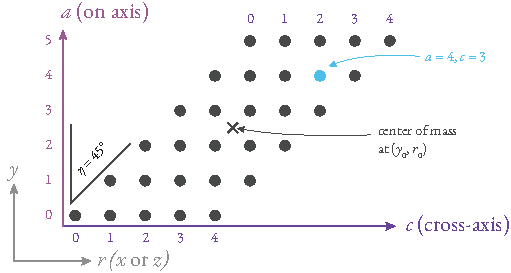
\includegraphics[scale=0.5]{\imagepath/coil_model/coil_model.pdf}
            \end{figure}
        \end{column}
    \end{columns}
    
    \pause
    \vspace{0.5cm}
    \begin{lstlisting}
collection = mpl.Collection()
current_factor = 1 if coil_index == 0 else -1  # opposite polarity on both sides
for row in range(self.windings_axis):
        on_axis_offset = (row - self.windings_axis/2 + 0.5) * winding_spacing
        for column in range(self.windings_cross_axis):
            radial_offset = np.tan(self.cone_angle)*on_axis_offset + (column - self.windings_cross_axis/2 + 0.5) * winding_spacing
            current = self.get_current(coil_index=coil_index, row=row, column=column)*current_factor
            loop = mpl.current.Loop(current=current, diameter=2*radius+2*radial_offset, position=(0, 0, on_axis_offset)
            collection.add(loop)
return collection
        \end{lstlisting}
\end{frame}


\begin{frame}
    \section*{Thank you!}
\end{frame}

\end{document}